\documentclass{article}
\usepackage{graphicx} % Required for inserting images
\usepackage{amsmath}
\usepackage{amssymb}
\usepackage{bm}
\usepackage{cancel}
\usepackage{algorithm}
\usepackage[noEnd=false,indLines=false]{algpseudocodex}
\usepackage[left=3.5cm, right=3.5cm]{geometry}
\usepackage{tikz}
\usepackage{tabu}
\usetikzlibrary{shapes,positioning,backgrounds, calc}
\usepackage{pgfplots}
\pgfplotsset{compat=newest }
\usepgfplotslibrary{external}
\tikzexternalize
\usepackage[style=ieee]{biblatex} %Imports biblatex package
\addbibresource{references.bib} %Import the bibliography file

\title{Polynomial approximation integration  \\ \large{Speeding up Neural Ordinary Differential Equations thought Parallelism} \\ v0.7}

\author{Yiorgos Panagiotopoulos}
\date{January 2023}

\begin{document}

    \maketitle


    \section{Introduction}
    The machine learning scene in 2023 is dominated by gargantuan models with billions of parameters.
    Even though they have demonstrated impressive results the compute and energy requirements of such models are a
    concern.
    It's the authors opinion that we ought to transition to analog or hybrid models of computation to reduce energy
    usage and increase speed.
    Even though digital computers are not going away any time soon studying alternative learning frameworks could ease
    the transition.

    Neural differential equations re-emerged in the recent years after~\cite{chen2018neural}.
    We believe they have great potential especially in modelling physical phenomena governed by differential equations,
    irregularly sampled time series and generative models like continuous normalising flows and stochastic differential
    equations.
    More importantly, in out opinion, they highlight a connection between deep learning and dynamical systems.
    Even thought we still operate in the discrete domain to use them in our current systems they offer an opportunity
    to close the gap between continuous time models and machine learning.

    We provide a quick overview of Neural ODES and propose a novel numerical integration method to tackle some of
    them limitations.


    \section{Residual Networks}
    In order to understand the intuition behind neural ordinary differential equations one should have a basic knowledge
    of residual networks.
    Residual networks, also known as ResNets, were introduced by He and others in their seminal
    paper~\cite{He_2016_CVPR}, to address the problem of \textit{degradation} in very deep architectures.
    It had become apparent by state of the art models of that time like~\cite{simonyan2014very} that depth plays a very
    important role in vision tasks, including classification.
    Stacking layers (depth) allows for the integration of low/mid/high level features in the learning process.
    The immediate obstacle in deep learning is the notorious vanishing gradient problem, but this has been largely
    solved through batch/group normalisation~\cite{ioffe2015batch}.

    It had been noticed though~\cite{srivastava2015highway}, that while stacking more layers, accuracy is initially saturated, unsurprisingly, but then it degrades rapidly.
    This degradation phenomenon is not caused by overfitting as the training error increases with the number of layers.
    ResNets solved this problem by utilising a residual learning framework.

    \subsection{Residual Learning}
    One can prove, by construction, that a deep architecture can be as accurate as a corresponding shallower one.
    This is achieved by adding identity layers in-between the layers of the shallower model.
    In more detail, consider a network that converges with some accuracy.
    Adding more layers to it would achieve the exact same accuracy if the extra layers learned to map their inputs straight to their outputs effectively making them identity mappings.
    The existence of this artificially deep network suggests that deep networks shouldn't produce higher error that the shallower ones.
    But the empirical evidence show that optimisers can't find this solution, at least in sensible time limits.

    \begin{center}
        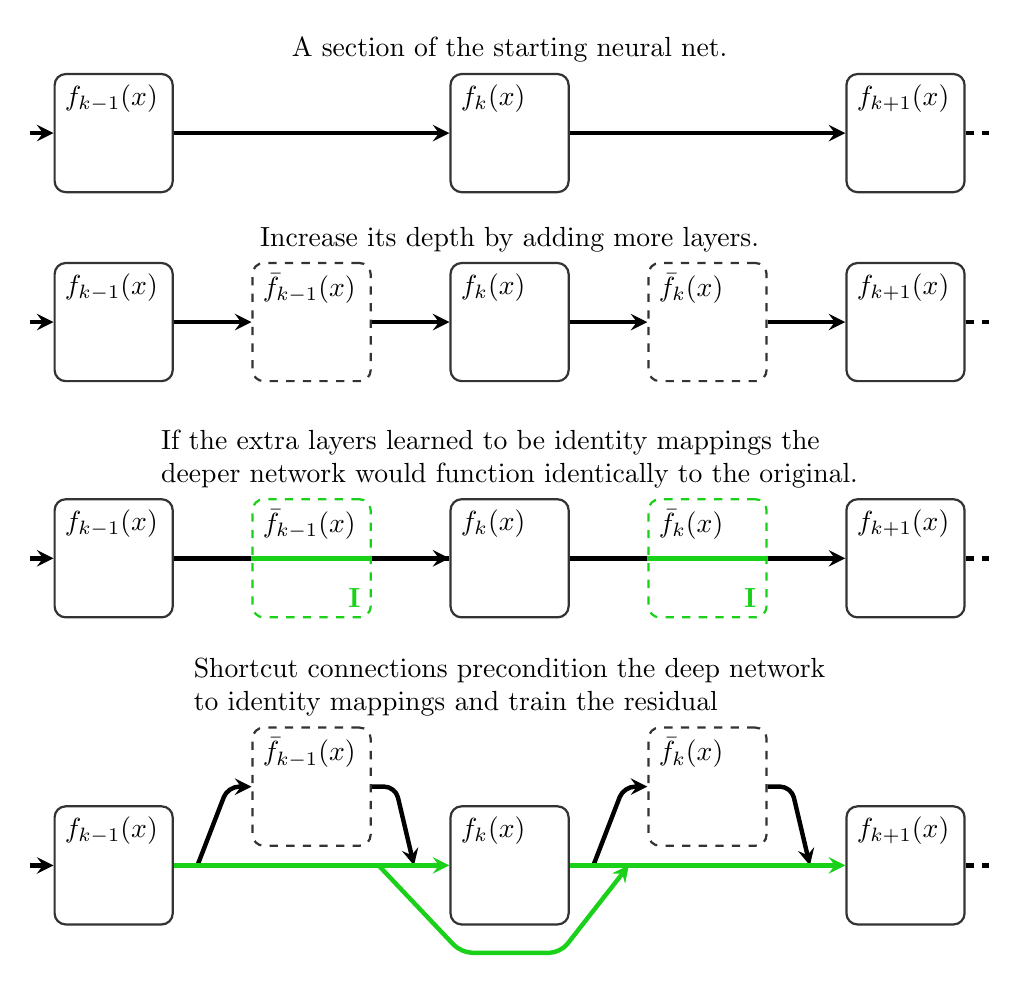
\begin{tikzpicture}[
            every path/.style={ultra thick},
            scale=3,
            block/.style={
                rectangle,
                rounded corners,
                thick,
                minimum size = 1.5cm,
                inner sep = 0pt,
                node distance = 3.5cm,
                draw=black!80
            },
            shallow/.style={
                block,
            },
            deep/.style={
                block,
                dashed,
                thick
            },
            darkgreen/.style={
                green!80!black!90
            },
            >= stealth,
        ]

            \begin{scope}[local bounding box = net1]
                \node[shallow] (A) at (0,0) {};
                \node[below right=0cm of A.north west] {$f_{k-1}(x)$};

                \node[shallow] (B) [right= of A] {};
                \node[below right=0cm of B.north west] {$f_{k}(x)$};

                \node[shallow] (C) [right= of B] {};
                \node[below right=0cm of C.north west] {$f_{k+1}(x)$};

                \draw[->] (A.west)+(-0.1cm,0) -- (A.west);
                \draw[->] (A.east) -- (B.west);
                \draw[->] (B.east) -- (C.west);
                \draw[dashed] (C.east) -- +(0.1cm,0);

                \node[above] at (current bounding box.north) {A section of the starting neural net.};

            \end{scope}

            \begin{scope}[local bounding box = scope1, yshift = -0.8cm]
                \node[shallow] (A) at (0,0) {};
                \node[below right=0cm of A.north west] {$f_{k-1}(x)$};

                \node[shallow] (B) [right= of A] {};
                \node[below right=0cm of B.north west] {$f_{k}(x)$};

                \node[shallow] (C) [right= of B] {};
                \node[below right=0cm of C.north west] {$f_{k+1}(x)$};

                \node[deep] (AB) at ($(A)!0.5!(B)$) {};
                \node[below right=0cm of AB.north west] {$\bar f_{k-1}(x)$};

                \node[deep] (BC) at ($(B)!0.5!(C)$) {};
                \node[below right=0cm of BC.north west] {$\bar f_{k}(x)$};

                \draw[->] (A.west)+(-0.1cm,0) -- (A.west);
                \draw[->] (A.east) -- (AB.west);
                \draw[->] (AB.east) -- (B.west);
                \draw[->] (B.east) -- (BC.west);
                \draw[->] (BC.east) -- (C.west);
                \draw[dashed] (C.east) -- +(0.1cm,0);

                \node[above] at (scope1.north) {Increase its depth by adding more layers.};
            \end{scope}

            \begin{scope}[local bounding box = scope2,yshift=-1.8cm]
                \node[shallow] (A) at (0,0) {};
                \node[below right=0cm of A.north west] {$f_{k-1}(x)$};

                \node[shallow] (B) [right= of A] {};
                \node[below right=0cm of B.north west] {$f_{k}(x)$};

                \node[shallow] (C) [right= of B] {};
                \node[below right=0cm of C.north west] {$f_{k+1}(x)$};

                \node[deep,darkgreen] (AB) at ($(A)!0.5!(B)$) {};
                \node[below right=0cm of AB.north west] {$\bar f_{k-1}(x)$};
                \node[above left=0cm of AB.south east, darkgreen] {$\mathbf I$};

                \node[deep,darkgreen] (BC) at ($(B)!0.5!(C)$) {};
                \node[below right=0cm of BC.north west] {$\bar f_{k}(x)$};
                \node[above left=0cm of BC.south east, darkgreen] {$ \mathbf I$};

                \draw[->] (A.west)+(-0.1cm,0) -- (A.west);
                \draw (A.east) -- (AB.west);
                \draw[darkgreen] (AB.west) -- (AB.east);
                \draw (AB.east) -- (B.west);
                \draw[->] (AB.east) -- (B.west);
                \draw (B.east) -- (BC.west);
                \draw[darkgreen] (BC.west) -- (BC.east);
                \draw[->] (BC.east) -- (C.west);
                \draw[dashed] (C.east) -- +(0.1cm,0);

                \node[above,align=left] at (scope2.north) {If the extra layers learned to be identity mappings the\\
                deeper network would function identically to the original.};
            \end{scope}

            \begin{scope}[local bounding box = scope3,yshift=-3.1cm]
                ;
                \node[shallow] (A) at (0,0) {};
                \node[below right=0cm of A.north west] {$f_{k-1}(x)$};

                \node[shallow] (B) [right= of A] {};
                \node[below right=0cm of B.north west] {$f_{k}(x)$};

                \node[shallow] (C) [right= of B] {};
                \node[below right=0cm of C.north west] {$f_{k+1}(x)$};

                \node[deep, yshift=1cm] (AB) at ($(A)!0.5!(B)$) {};
                \node[below right=0cm of AB.north west] {$\bar f_{k-1}(x)$};
                \node[above left=0cm of AB.south east] {};

                \node[deep, yshift=1cm] (BC) at ($(B)!0.5!(C)$) {};
                \node[below right=0cm of BC.north west] {$\bar f_{k}(x)$};
                \node[above left=0cm of BC.south east] {};

                \draw[->] (A.west)+(-0.1cm,0) -- (A.west);
                \draw[->, rounded corners] (A.east) +(0.1cm,0) -- ($(AB.west) - (0.1cm,0)$)  -- (AB.west);
                \draw[->, rounded corners] (AB.east) -- ++(0.1cm,0) -- ($(B.west) + (-0.15cm,0)$);
                \draw[->, rounded corners] (B.east) +(0.1cm,0) -- ($(BC.west) - (0.1cm,0)$)  -- (BC.west);
                \draw[->, rounded corners] (BC.east) -- ++(0.1cm,0) -- ($(C.west) + (-0.15cm,0)$);
                \draw[dashed] (C.east) -- +(0.1cm,0);

                \draw[->,darkgreen, rounded corners] (B.west) +(-0.3cm,0) -- ++(0.05cm, -0.37cm) -- ++(0.42cm, 0cm) -- ($(B.east) + (0.25cm,0)$);
                \draw[->,darkgreen] (A.east) -- (B.west);
                \draw[->,darkgreen] (B.east) -- (C.west);

                \node[above,align=left] at (scope3.north) {Shortcut connections precondition the deep network \\ to identity mappings and train the residual };
            \end{scope}
        \end{tikzpicture}
    \end{center}

    In order to incorporate this observation into the network, so called \textit{shortcut connections} are introduced to the layers.
    Basically, the input to a block of stacked layers is added back to it's output.
    This way the network instead of learning the direct mapping $\mathcal{H}(x) = \mathcal{F}(x)$, it learns the residual mapping $\mathcal{H}(x) = \mathcal{R}(x)+x$.
    The optimiser can then push the residual mappings to $0$ leading to identity connections.
    Even though identity mappings are unlikely to be optimum, experiments showed that the residual connections have generally small responses, meaning identities are good pre-conditioners for deep architectures.

    Since their conception Residual Networks have revolutionised deep learning allowing for much deeper architectures than previously used.
    Furthermore, the idea of residual learning has found vast appeal in many other architectures.
    Transformers for example, employ residual connections, allowing many such layers to be stacked creating large expressive models~\cite{vaswani2017attention}.


    \section{Neural ODEs}
    There exist examples in the literature of combining neural networks and dynamical systems, even since the 1990s~\cite{rico1992discrete}.
    Interest began to increase after the publication of ResNet~\cite{weinan2018mean}.
    But the field of Neural Differential Equations really became prominent with~\cite{chen2018neural}.

    \subsection{A continuous time network}
    Let's revisit Residual Networks and how they work.
    The input-output relationship of the $k$-th ResNet block is given by:
    \begin{equation}
        \pmb{y}_{k+1} = \pmb{y}_{k} + f(\pmb{y}_{k}; \pmb{\theta}_k) \label{resnet}
    \end{equation}
    where $\pmb{y}_{k+1} \in \mathbb{R}^{N_y}$ is the output of the block, $\pmb{y}^{k} \in \mathbb{R}^{N_y}$ is its input and $f$ is a fully connected layer with parameters $\pmb{\theta}_k \in \mathbb{R}^{N_\theta}$.
    Notice that we refer to ResNet blocks, not layers, since residual connections are generally not between the input and output of a single linear layer but a stack of them; from now on we will use the terms interchangeably.

    The update in the \textit{hidden state} $\pmb{y}$ in~\eqref{resnet} resembles the formula of the forward Euler iteration for solving ordinary differential equations.
    This observation led the authors of~\cite{lu2018beyond} [CITE MORE] to make a connection between some neural network architectures and differential equations.
    Suppose that we could keep increasing the depth of the ResNet in~\eqref{resnet} while the time of the forward pass remained bounded, meaning each layer would take less and less time.
    In the limit we get a differential equation governed by the dynamics defined by a neural network $f$.
    \begin{equation}
        \frac{ \pmb{y}(t)}{dt} = f(\pmb{y}(t); \pmb{\theta}) \label{diffeq}
    \end{equation}
    Instead of a discrete sequence of hidden states, $\pmb{y}(t)$ is a continuous flow $\pmb{y} : [0,T] \to \mathbb{R}^{N_y}$ defined be the vector field parameterised by $\pmb{\theta}$.

    One important issue we haven't addressed is that the weights in~\eqref{resnet} change at each layer but at~\eqref{diffeq} they are the same for the entire trajectory.
    For notations sake we could define $f$ as $f(\pmb{y}(t), t, \pmb{\theta})$ meaning at certain ``depths'' different sections of the weights vector $\pmb{\theta}$ are used, maybe in a piecewise constant fashion~\cite{kidger2022neural}.
    Alternatively, the weights could be time dependant which complicates the model but leads to \textit{Galerkin} Neural ODEs, a more suitable continuous time equivalent of ResNet~\cite{massaroli2020dissecting}.
    For our purposes we consider the weights constant for the rest of this paper.

    \subsection{Inference}
    Under this new machine learning framework depth is replaced by time.
    Inference is performed by solving an initial value problem from initial time $t=0$ to terminal time $t=T$.
    \begin{equation}
        \pmb{y}(T) = \pmb{y}(0) + \int_{0}^{T} f(\pmb{y}(\tau); \pmb{\theta}) \, d\tau \label{ivp}
    \end{equation}

    Obviously,~\eqref{ivp} is a continuous time problem while our computers work in discrete time \textit{(for now)}.
    In order to solve it we employ a numerical method for solving \textit{Initial Value Problems}, .
    If we were to use forward Euler, an explicit method, we would get a recurrence relation of the form
    \begin{equation}
        \pmb{y}(t_k + h) = \pmb{y}(t_k) + h \left. \frac{d\pmb{y}(t)}{dt} \right|_{t = t_k}
        \label{forwaredEu}
    \end{equation}
    By considering that $\frac{d \pmb{y}(t)}{dt} = f(\pmb{y}(t);\pmb{\theta})$ eq. \eqref{forwaredEu} can be written as:
    \begin{equation}
        \pmb{y}(t_k + h) = \pmb{y}(t_k) + h f(\pmb{y}(t_k); \pmb{\theta} )
        \label{res2eul}
    \end{equation}
    which coincides with the ResNet formula.
    Many other neural network architectures can be interpreted as solving a neural ODE using different methods~\cite{chen2019ordinary}.
    The field of numerical differential equation solvers is quite vast meaning one could choose one that fits his specifications.
    A notable case is that of adaptive solvers like Runge-Kutta-Fehlberg (RKF45), that use varying step sizes.
    This way to obtain  $\pmb{y}(T)$ the solver may require different number of $f$ evaluations depending on the input and the complexity of the vector field at that input.
    For simple dynamics the solver can ``decide'' to use large step sizes meaning fewer function evaluations.
    Otherwise when the the vector field is more complex, a smaller step size will be used -to reduce error- leading to more function evaluations.
    We could interpret this behaviour as a network of ``variable depth''.

    It's important to clarify here that there are effectively two networks at play.
    Firstly, there is $f$, inherited from a block or layer of the original formulation of the problem.
    It is a neural network in the classical sense comprised of matrix vector multiplications and non-linearities.
    Secondly, there is the outlining model, the neural differential equation, which receives input $\pmb{y}_0$ and produced output $\pmb{y}(T)$; $f$ is to neural ODE what a layer is to ResNet.
    Internally, depending on the solver, $f$ will be evaluated for many values of $\pmb{y}(t)$.
    As disguised above, in contrast to ResNet $f$ contains all the learnable parameters of the model, which in out case are independent of depth.
    In conclusion the Neural ODE is comprised of: a neural network $f$ -that defines a \textit{learnable} vector field- parameterised by $\pmb{\theta}$,  some input $y_0$ and a numerical solver that applies $f$ until it reaches $\pmb{y}(T)$.

    \begin{figure}[h]
        \begin{center}
            %% Creator: Matplotlib, PGF backend
%%
%% To include the figure in your LaTeX document, write
%%   \input{<filename>.pgf}
%%
%% Make sure the required packages are loaded in your preamble
%%   \usepackage{pgf}
%%
%% Also ensure that all the required font packages are loaded; for instance,
%% the lmodern package is sometimes necessary when using math font.
%%   \usepackage{lmodern}
%%
%% Figures using additional raster images can only be included by \input if
%% they are in the same directory as the main LaTeX file. For loading figures
%% from other directories you can use the `import` package
%%   \usepackage{import}
%%
%% and then include the figures with
%%   \import{<path to file>}{<filename>.pgf}
%%
%% Matplotlib used the following preamble
%%   
%%   \makeatletter\@ifpackageloaded{underscore}{}{\usepackage[strings]{underscore}}\makeatother
%%
\begingroup%
\makeatletter%
\begin{pgfpicture}%
\pgfpathrectangle{\pgfpointorigin}{\pgfqpoint{4.724409in}{4.724409in}}%
\pgfusepath{use as bounding box, clip}%
\begin{pgfscope}%
\pgfsetbuttcap%
\pgfsetmiterjoin%
\definecolor{currentfill}{rgb}{1.000000,1.000000,1.000000}%
\pgfsetfillcolor{currentfill}%
\pgfsetlinewidth{0.000000pt}%
\definecolor{currentstroke}{rgb}{1.000000,1.000000,1.000000}%
\pgfsetstrokecolor{currentstroke}%
\pgfsetdash{}{0pt}%
\pgfpathmoveto{\pgfqpoint{0.000000in}{0.000000in}}%
\pgfpathlineto{\pgfqpoint{4.724409in}{0.000000in}}%
\pgfpathlineto{\pgfqpoint{4.724409in}{4.724409in}}%
\pgfpathlineto{\pgfqpoint{0.000000in}{4.724409in}}%
\pgfpathlineto{\pgfqpoint{0.000000in}{0.000000in}}%
\pgfpathclose%
\pgfusepath{fill}%
\end{pgfscope}%
\begin{pgfscope}%
\pgfsetbuttcap%
\pgfsetmiterjoin%
\definecolor{currentfill}{rgb}{1.000000,1.000000,1.000000}%
\pgfsetfillcolor{currentfill}%
\pgfsetlinewidth{0.000000pt}%
\definecolor{currentstroke}{rgb}{0.000000,0.000000,0.000000}%
\pgfsetstrokecolor{currentstroke}%
\pgfsetstrokeopacity{0.000000}%
\pgfsetdash{}{0pt}%
\pgfpathmoveto{\pgfqpoint{0.329012in}{2.564365in}}%
\pgfpathlineto{\pgfqpoint{2.287205in}{2.564365in}}%
\pgfpathlineto{\pgfqpoint{2.287205in}{4.276262in}}%
\pgfpathlineto{\pgfqpoint{0.329012in}{4.276262in}}%
\pgfpathlineto{\pgfqpoint{0.329012in}{2.564365in}}%
\pgfpathclose%
\pgfusepath{fill}%
\end{pgfscope}%
\begin{pgfscope}%
\pgfsetbuttcap%
\pgfsetroundjoin%
\definecolor{currentfill}{rgb}{0.000000,0.000000,0.000000}%
\pgfsetfillcolor{currentfill}%
\pgfsetlinewidth{0.803000pt}%
\definecolor{currentstroke}{rgb}{0.000000,0.000000,0.000000}%
\pgfsetstrokecolor{currentstroke}%
\pgfsetdash{}{0pt}%
\pgfsys@defobject{currentmarker}{\pgfqpoint{0.000000in}{-0.048611in}}{\pgfqpoint{0.000000in}{0.000000in}}{%
\pgfpathmoveto{\pgfqpoint{0.000000in}{0.000000in}}%
\pgfpathlineto{\pgfqpoint{0.000000in}{-0.048611in}}%
\pgfusepath{stroke,fill}%
}%
\begin{pgfscope}%
\pgfsys@transformshift{0.329012in}{2.564365in}%
\pgfsys@useobject{currentmarker}{}%
\end{pgfscope}%
\end{pgfscope}%
\begin{pgfscope}%
\pgfsetbuttcap%
\pgfsetroundjoin%
\definecolor{currentfill}{rgb}{0.000000,0.000000,0.000000}%
\pgfsetfillcolor{currentfill}%
\pgfsetlinewidth{0.803000pt}%
\definecolor{currentstroke}{rgb}{0.000000,0.000000,0.000000}%
\pgfsetstrokecolor{currentstroke}%
\pgfsetdash{}{0pt}%
\pgfsys@defobject{currentmarker}{\pgfqpoint{0.000000in}{-0.048611in}}{\pgfqpoint{0.000000in}{0.000000in}}{%
\pgfpathmoveto{\pgfqpoint{0.000000in}{0.000000in}}%
\pgfpathlineto{\pgfqpoint{0.000000in}{-0.048611in}}%
\pgfusepath{stroke,fill}%
}%
\begin{pgfscope}%
\pgfsys@transformshift{0.684148in}{2.564365in}%
\pgfsys@useobject{currentmarker}{}%
\end{pgfscope}%
\end{pgfscope}%
\begin{pgfscope}%
\pgfsetbuttcap%
\pgfsetroundjoin%
\definecolor{currentfill}{rgb}{0.000000,0.000000,0.000000}%
\pgfsetfillcolor{currentfill}%
\pgfsetlinewidth{0.803000pt}%
\definecolor{currentstroke}{rgb}{0.000000,0.000000,0.000000}%
\pgfsetstrokecolor{currentstroke}%
\pgfsetdash{}{0pt}%
\pgfsys@defobject{currentmarker}{\pgfqpoint{0.000000in}{-0.048611in}}{\pgfqpoint{0.000000in}{0.000000in}}{%
\pgfpathmoveto{\pgfqpoint{0.000000in}{0.000000in}}%
\pgfpathlineto{\pgfqpoint{0.000000in}{-0.048611in}}%
\pgfusepath{stroke,fill}%
}%
\begin{pgfscope}%
\pgfsys@transformshift{1.103705in}{2.564365in}%
\pgfsys@useobject{currentmarker}{}%
\end{pgfscope}%
\end{pgfscope}%
\begin{pgfscope}%
\pgfsetbuttcap%
\pgfsetroundjoin%
\definecolor{currentfill}{rgb}{0.000000,0.000000,0.000000}%
\pgfsetfillcolor{currentfill}%
\pgfsetlinewidth{0.803000pt}%
\definecolor{currentstroke}{rgb}{0.000000,0.000000,0.000000}%
\pgfsetstrokecolor{currentstroke}%
\pgfsetdash{}{0pt}%
\pgfsys@defobject{currentmarker}{\pgfqpoint{0.000000in}{-0.048611in}}{\pgfqpoint{0.000000in}{0.000000in}}{%
\pgfpathmoveto{\pgfqpoint{0.000000in}{0.000000in}}%
\pgfpathlineto{\pgfqpoint{0.000000in}{-0.048611in}}%
\pgfusepath{stroke,fill}%
}%
\begin{pgfscope}%
\pgfsys@transformshift{1.599350in}{2.564365in}%
\pgfsys@useobject{currentmarker}{}%
\end{pgfscope}%
\end{pgfscope}%
\begin{pgfscope}%
\pgfsetbuttcap%
\pgfsetroundjoin%
\definecolor{currentfill}{rgb}{0.000000,0.000000,0.000000}%
\pgfsetfillcolor{currentfill}%
\pgfsetlinewidth{0.803000pt}%
\definecolor{currentstroke}{rgb}{0.000000,0.000000,0.000000}%
\pgfsetstrokecolor{currentstroke}%
\pgfsetdash{}{0pt}%
\pgfsys@defobject{currentmarker}{\pgfqpoint{0.000000in}{-0.048611in}}{\pgfqpoint{0.000000in}{0.000000in}}{%
\pgfpathmoveto{\pgfqpoint{0.000000in}{0.000000in}}%
\pgfpathlineto{\pgfqpoint{0.000000in}{-0.048611in}}%
\pgfusepath{stroke,fill}%
}%
\begin{pgfscope}%
\pgfsys@transformshift{2.184884in}{2.564365in}%
\pgfsys@useobject{currentmarker}{}%
\end{pgfscope}%
\end{pgfscope}%
\begin{pgfscope}%
\definecolor{textcolor}{rgb}{0.000000,0.000000,0.000000}%
\pgfsetstrokecolor{textcolor}%
\pgfsetfillcolor{textcolor}%
\pgftext[x=1.308108in,y=2.411588in,,top]{\color{textcolor}\rmfamily\fontsize{10.000000}{12.000000}\selectfont depth}%
\end{pgfscope}%
\begin{pgfscope}%
\definecolor{textcolor}{rgb}{0.000000,0.000000,0.000000}%
\pgfsetstrokecolor{textcolor}%
\pgfsetfillcolor{textcolor}%
\pgftext[x=0.273457in,y=3.420314in,,bottom,rotate=90.000000]{\color{textcolor}\rmfamily\fontsize{10.000000}{12.000000}\selectfont state}%
\end{pgfscope}%
\begin{pgfscope}%
\pgfpathrectangle{\pgfqpoint{0.329012in}{2.564365in}}{\pgfqpoint{1.958193in}{1.711897in}}%
\pgfusepath{clip}%
\pgfsetbuttcap%
\pgfsetroundjoin%
\pgfsetlinewidth{0.602250pt}%
\definecolor{currentstroke}{rgb}{0.333333,0.333333,0.333333}%
\pgfsetstrokecolor{currentstroke}%
\pgfsetstrokeopacity{0.062745}%
\pgfsetdash{}{0pt}%
\pgfpathmoveto{\pgfqpoint{0.329012in}{2.589432in}}%
\pgfpathlineto{\pgfqpoint{0.353552in}{2.588623in}}%
\pgfusepath{stroke}%
\end{pgfscope}%
\begin{pgfscope}%
\pgfpathrectangle{\pgfqpoint{0.329012in}{2.564365in}}{\pgfqpoint{1.958193in}{1.711897in}}%
\pgfusepath{clip}%
\pgfsetbuttcap%
\pgfsetroundjoin%
\pgfsetlinewidth{0.602250pt}%
\definecolor{currentstroke}{rgb}{0.333333,0.333333,0.333333}%
\pgfsetstrokecolor{currentstroke}%
\pgfsetstrokeopacity{0.062745}%
\pgfsetdash{}{0pt}%
\pgfpathmoveto{\pgfqpoint{0.353552in}{2.588623in}}%
\pgfpathlineto{\pgfqpoint{0.433968in}{2.581809in}}%
\pgfusepath{stroke}%
\end{pgfscope}%
\begin{pgfscope}%
\pgfpathrectangle{\pgfqpoint{0.329012in}{2.564365in}}{\pgfqpoint{1.958193in}{1.711897in}}%
\pgfusepath{clip}%
\pgfsetbuttcap%
\pgfsetroundjoin%
\pgfsetlinewidth{0.602250pt}%
\definecolor{currentstroke}{rgb}{0.333333,0.333333,0.333333}%
\pgfsetstrokecolor{currentstroke}%
\pgfsetstrokeopacity{0.062745}%
\pgfsetdash{}{0pt}%
\pgfpathmoveto{\pgfqpoint{0.433968in}{2.581809in}}%
\pgfpathlineto{\pgfqpoint{0.524831in}{2.564365in}}%
\pgfusepath{stroke}%
\end{pgfscope}%
\begin{pgfscope}%
\pgfpathrectangle{\pgfqpoint{0.329012in}{2.564365in}}{\pgfqpoint{1.958193in}{1.711897in}}%
\pgfusepath{clip}%
\pgfsetbuttcap%
\pgfsetroundjoin%
\pgfsetlinewidth{0.602250pt}%
\definecolor{currentstroke}{rgb}{0.333333,0.333333,0.333333}%
\pgfsetstrokecolor{currentstroke}%
\pgfsetstrokeopacity{0.062745}%
\pgfsetdash{}{0pt}%
\pgfpathmoveto{\pgfqpoint{0.524831in}{2.564365in}}%
\pgfpathlineto{\pgfqpoint{0.524831in}{2.564365in}}%
\pgfusepath{stroke}%
\end{pgfscope}%
\begin{pgfscope}%
\pgfpathrectangle{\pgfqpoint{0.329012in}{2.564365in}}{\pgfqpoint{1.958193in}{1.711897in}}%
\pgfusepath{clip}%
\pgfsetbuttcap%
\pgfsetroundjoin%
\pgfsetlinewidth{0.602250pt}%
\definecolor{currentstroke}{rgb}{0.333333,0.333333,0.333333}%
\pgfsetstrokecolor{currentstroke}%
\pgfsetstrokeopacity{0.062745}%
\pgfsetdash{}{0pt}%
\pgfpathmoveto{\pgfqpoint{0.329012in}{2.654594in}}%
\pgfpathlineto{\pgfqpoint{0.377265in}{2.651736in}}%
\pgfusepath{stroke}%
\end{pgfscope}%
\begin{pgfscope}%
\pgfpathrectangle{\pgfqpoint{0.329012in}{2.564365in}}{\pgfqpoint{1.958193in}{1.711897in}}%
\pgfusepath{clip}%
\pgfsetbuttcap%
\pgfsetroundjoin%
\pgfsetlinewidth{0.602250pt}%
\definecolor{currentstroke}{rgb}{0.333333,0.333333,0.333333}%
\pgfsetstrokecolor{currentstroke}%
\pgfsetstrokeopacity{0.062745}%
\pgfsetdash{}{0pt}%
\pgfpathmoveto{\pgfqpoint{0.377265in}{2.651736in}}%
\pgfpathlineto{\pgfqpoint{0.461258in}{2.642652in}}%
\pgfusepath{stroke}%
\end{pgfscope}%
\begin{pgfscope}%
\pgfpathrectangle{\pgfqpoint{0.329012in}{2.564365in}}{\pgfqpoint{1.958193in}{1.711897in}}%
\pgfusepath{clip}%
\pgfsetbuttcap%
\pgfsetroundjoin%
\pgfsetlinewidth{0.602250pt}%
\definecolor{currentstroke}{rgb}{0.333333,0.333333,0.333333}%
\pgfsetstrokecolor{currentstroke}%
\pgfsetstrokeopacity{0.062745}%
\pgfsetdash{}{0pt}%
\pgfpathmoveto{\pgfqpoint{0.461258in}{2.642652in}}%
\pgfpathlineto{\pgfqpoint{0.547985in}{2.624810in}}%
\pgfusepath{stroke}%
\end{pgfscope}%
\begin{pgfscope}%
\pgfpathrectangle{\pgfqpoint{0.329012in}{2.564365in}}{\pgfqpoint{1.958193in}{1.711897in}}%
\pgfusepath{clip}%
\pgfsetbuttcap%
\pgfsetroundjoin%
\pgfsetlinewidth{0.602250pt}%
\definecolor{currentstroke}{rgb}{0.333333,0.333333,0.333333}%
\pgfsetstrokecolor{currentstroke}%
\pgfsetstrokeopacity{0.062745}%
\pgfsetdash{}{0pt}%
\pgfpathmoveto{\pgfqpoint{0.547985in}{2.624810in}}%
\pgfpathlineto{\pgfqpoint{0.635932in}{2.598153in}}%
\pgfusepath{stroke}%
\end{pgfscope}%
\begin{pgfscope}%
\pgfpathrectangle{\pgfqpoint{0.329012in}{2.564365in}}{\pgfqpoint{1.958193in}{1.711897in}}%
\pgfusepath{clip}%
\pgfsetbuttcap%
\pgfsetroundjoin%
\pgfsetlinewidth{0.602250pt}%
\definecolor{currentstroke}{rgb}{0.333333,0.333333,0.333333}%
\pgfsetstrokecolor{currentstroke}%
\pgfsetstrokeopacity{0.062745}%
\pgfsetdash{}{0pt}%
\pgfpathmoveto{\pgfqpoint{0.635932in}{2.598153in}}%
\pgfpathlineto{\pgfqpoint{0.720651in}{2.564365in}}%
\pgfusepath{stroke}%
\end{pgfscope}%
\begin{pgfscope}%
\pgfpathrectangle{\pgfqpoint{0.329012in}{2.564365in}}{\pgfqpoint{1.958193in}{1.711897in}}%
\pgfusepath{clip}%
\pgfsetbuttcap%
\pgfsetroundjoin%
\pgfsetlinewidth{0.602250pt}%
\definecolor{currentstroke}{rgb}{0.333333,0.333333,0.333333}%
\pgfsetstrokecolor{currentstroke}%
\pgfsetstrokeopacity{0.062745}%
\pgfsetdash{}{0pt}%
\pgfpathmoveto{\pgfqpoint{0.720651in}{2.564365in}}%
\pgfpathlineto{\pgfqpoint{0.720651in}{2.564365in}}%
\pgfusepath{stroke}%
\end{pgfscope}%
\begin{pgfscope}%
\pgfpathrectangle{\pgfqpoint{0.329012in}{2.564365in}}{\pgfqpoint{1.958193in}{1.711897in}}%
\pgfusepath{clip}%
\pgfsetbuttcap%
\pgfsetroundjoin%
\pgfsetlinewidth{0.602250pt}%
\definecolor{currentstroke}{rgb}{0.333333,0.333333,0.333333}%
\pgfsetstrokecolor{currentstroke}%
\pgfsetstrokeopacity{0.062745}%
\pgfsetdash{}{0pt}%
\pgfpathmoveto{\pgfqpoint{0.329012in}{2.743593in}}%
\pgfpathlineto{\pgfqpoint{0.403353in}{2.737644in}}%
\pgfusepath{stroke}%
\end{pgfscope}%
\begin{pgfscope}%
\pgfpathrectangle{\pgfqpoint{0.329012in}{2.564365in}}{\pgfqpoint{1.958193in}{1.711897in}}%
\pgfusepath{clip}%
\pgfsetbuttcap%
\pgfsetroundjoin%
\pgfsetlinewidth{0.602250pt}%
\definecolor{currentstroke}{rgb}{0.333333,0.333333,0.333333}%
\pgfsetstrokecolor{currentstroke}%
\pgfsetstrokeopacity{0.062745}%
\pgfsetdash{}{0pt}%
\pgfpathmoveto{\pgfqpoint{0.403353in}{2.737644in}}%
\pgfpathlineto{\pgfqpoint{0.492875in}{2.726413in}}%
\pgfusepath{stroke}%
\end{pgfscope}%
\begin{pgfscope}%
\pgfpathrectangle{\pgfqpoint{0.329012in}{2.564365in}}{\pgfqpoint{1.958193in}{1.711897in}}%
\pgfusepath{clip}%
\pgfsetbuttcap%
\pgfsetroundjoin%
\pgfsetlinewidth{0.602250pt}%
\definecolor{currentstroke}{rgb}{0.333333,0.333333,0.333333}%
\pgfsetstrokecolor{currentstroke}%
\pgfsetstrokeopacity{0.062745}%
\pgfsetdash{}{0pt}%
\pgfpathmoveto{\pgfqpoint{0.492875in}{2.726413in}}%
\pgfpathlineto{\pgfqpoint{0.583178in}{2.706941in}}%
\pgfusepath{stroke}%
\end{pgfscope}%
\begin{pgfscope}%
\pgfpathrectangle{\pgfqpoint{0.329012in}{2.564365in}}{\pgfqpoint{1.958193in}{1.711897in}}%
\pgfusepath{clip}%
\pgfsetbuttcap%
\pgfsetroundjoin%
\pgfsetlinewidth{0.602250pt}%
\definecolor{currentstroke}{rgb}{0.333333,0.333333,0.333333}%
\pgfsetstrokecolor{currentstroke}%
\pgfsetstrokeopacity{0.062745}%
\pgfsetdash{}{0pt}%
\pgfpathmoveto{\pgfqpoint{0.583178in}{2.706941in}}%
\pgfpathlineto{\pgfqpoint{0.671074in}{2.680239in}}%
\pgfusepath{stroke}%
\end{pgfscope}%
\begin{pgfscope}%
\pgfpathrectangle{\pgfqpoint{0.329012in}{2.564365in}}{\pgfqpoint{1.958193in}{1.711897in}}%
\pgfusepath{clip}%
\pgfsetbuttcap%
\pgfsetroundjoin%
\pgfsetlinewidth{0.602250pt}%
\definecolor{currentstroke}{rgb}{0.333333,0.333333,0.333333}%
\pgfsetstrokecolor{currentstroke}%
\pgfsetstrokeopacity{0.062745}%
\pgfsetdash{}{0pt}%
\pgfpathmoveto{\pgfqpoint{0.671074in}{2.680239in}}%
\pgfpathlineto{\pgfqpoint{0.756100in}{2.647071in}}%
\pgfusepath{stroke}%
\end{pgfscope}%
\begin{pgfscope}%
\pgfpathrectangle{\pgfqpoint{0.329012in}{2.564365in}}{\pgfqpoint{1.958193in}{1.711897in}}%
\pgfusepath{clip}%
\pgfsetbuttcap%
\pgfsetroundjoin%
\pgfsetlinewidth{0.602250pt}%
\definecolor{currentstroke}{rgb}{0.333333,0.333333,0.333333}%
\pgfsetstrokecolor{currentstroke}%
\pgfsetstrokeopacity{0.062745}%
\pgfsetdash{}{0pt}%
\pgfpathmoveto{\pgfqpoint{0.756100in}{2.647071in}}%
\pgfpathlineto{\pgfqpoint{0.837944in}{2.608191in}}%
\pgfusepath{stroke}%
\end{pgfscope}%
\begin{pgfscope}%
\pgfpathrectangle{\pgfqpoint{0.329012in}{2.564365in}}{\pgfqpoint{1.958193in}{1.711897in}}%
\pgfusepath{clip}%
\pgfsetbuttcap%
\pgfsetroundjoin%
\pgfsetlinewidth{0.602250pt}%
\definecolor{currentstroke}{rgb}{0.333333,0.333333,0.333333}%
\pgfsetstrokecolor{currentstroke}%
\pgfsetstrokeopacity{0.062745}%
\pgfsetdash{}{0pt}%
\pgfpathmoveto{\pgfqpoint{0.837944in}{2.608191in}}%
\pgfpathlineto{\pgfqpoint{0.916470in}{2.564365in}}%
\pgfusepath{stroke}%
\end{pgfscope}%
\begin{pgfscope}%
\pgfpathrectangle{\pgfqpoint{0.329012in}{2.564365in}}{\pgfqpoint{1.958193in}{1.711897in}}%
\pgfusepath{clip}%
\pgfsetbuttcap%
\pgfsetroundjoin%
\pgfsetlinewidth{0.602250pt}%
\definecolor{currentstroke}{rgb}{0.333333,0.333333,0.333333}%
\pgfsetstrokecolor{currentstroke}%
\pgfsetstrokeopacity{0.062745}%
\pgfsetdash{}{0pt}%
\pgfpathmoveto{\pgfqpoint{0.916470in}{2.564365in}}%
\pgfpathlineto{\pgfqpoint{0.916470in}{2.564365in}}%
\pgfusepath{stroke}%
\end{pgfscope}%
\begin{pgfscope}%
\pgfpathrectangle{\pgfqpoint{0.329012in}{2.564365in}}{\pgfqpoint{1.958193in}{1.711897in}}%
\pgfusepath{clip}%
\pgfsetbuttcap%
\pgfsetroundjoin%
\pgfsetlinewidth{0.602250pt}%
\definecolor{currentstroke}{rgb}{0.333333,0.333333,0.333333}%
\pgfsetstrokecolor{currentstroke}%
\pgfsetstrokeopacity{0.062745}%
\pgfsetdash{}{0pt}%
\pgfpathmoveto{\pgfqpoint{0.329012in}{2.837498in}}%
\pgfpathlineto{\pgfqpoint{0.350513in}{2.837062in}}%
\pgfusepath{stroke}%
\end{pgfscope}%
\begin{pgfscope}%
\pgfpathrectangle{\pgfqpoint{0.329012in}{2.564365in}}{\pgfqpoint{1.958193in}{1.711897in}}%
\pgfusepath{clip}%
\pgfsetbuttcap%
\pgfsetroundjoin%
\pgfsetlinewidth{0.602250pt}%
\definecolor{currentstroke}{rgb}{0.333333,0.333333,0.333333}%
\pgfsetstrokecolor{currentstroke}%
\pgfsetstrokeopacity{0.062745}%
\pgfsetdash{}{0pt}%
\pgfpathmoveto{\pgfqpoint{0.350513in}{2.837062in}}%
\pgfpathlineto{\pgfqpoint{0.443353in}{2.831290in}}%
\pgfusepath{stroke}%
\end{pgfscope}%
\begin{pgfscope}%
\pgfpathrectangle{\pgfqpoint{0.329012in}{2.564365in}}{\pgfqpoint{1.958193in}{1.711897in}}%
\pgfusepath{clip}%
\pgfsetbuttcap%
\pgfsetroundjoin%
\pgfsetlinewidth{0.602250pt}%
\definecolor{currentstroke}{rgb}{0.333333,0.333333,0.333333}%
\pgfsetstrokecolor{currentstroke}%
\pgfsetstrokeopacity{0.062745}%
\pgfsetdash{}{0pt}%
\pgfpathmoveto{\pgfqpoint{0.443353in}{2.831290in}}%
\pgfpathlineto{\pgfqpoint{0.535254in}{2.818102in}}%
\pgfusepath{stroke}%
\end{pgfscope}%
\begin{pgfscope}%
\pgfpathrectangle{\pgfqpoint{0.329012in}{2.564365in}}{\pgfqpoint{1.958193in}{1.711897in}}%
\pgfusepath{clip}%
\pgfsetbuttcap%
\pgfsetroundjoin%
\pgfsetlinewidth{0.602250pt}%
\definecolor{currentstroke}{rgb}{0.333333,0.333333,0.333333}%
\pgfsetstrokecolor{currentstroke}%
\pgfsetstrokeopacity{0.062745}%
\pgfsetdash{}{0pt}%
\pgfpathmoveto{\pgfqpoint{0.535254in}{2.818102in}}%
\pgfpathlineto{\pgfqpoint{0.625537in}{2.798102in}}%
\pgfusepath{stroke}%
\end{pgfscope}%
\begin{pgfscope}%
\pgfpathrectangle{\pgfqpoint{0.329012in}{2.564365in}}{\pgfqpoint{1.958193in}{1.711897in}}%
\pgfusepath{clip}%
\pgfsetbuttcap%
\pgfsetroundjoin%
\pgfsetlinewidth{0.602250pt}%
\definecolor{currentstroke}{rgb}{0.333333,0.333333,0.333333}%
\pgfsetstrokecolor{currentstroke}%
\pgfsetstrokeopacity{0.062745}%
\pgfsetdash{}{0pt}%
\pgfpathmoveto{\pgfqpoint{0.625537in}{2.798102in}}%
\pgfpathlineto{\pgfqpoint{0.713670in}{2.771833in}}%
\pgfusepath{stroke}%
\end{pgfscope}%
\begin{pgfscope}%
\pgfpathrectangle{\pgfqpoint{0.329012in}{2.564365in}}{\pgfqpoint{1.958193in}{1.711897in}}%
\pgfusepath{clip}%
\pgfsetbuttcap%
\pgfsetroundjoin%
\pgfsetlinewidth{0.602250pt}%
\definecolor{currentstroke}{rgb}{0.333333,0.333333,0.333333}%
\pgfsetstrokecolor{currentstroke}%
\pgfsetstrokeopacity{0.062745}%
\pgfsetdash{}{0pt}%
\pgfpathmoveto{\pgfqpoint{0.713670in}{2.771833in}}%
\pgfpathlineto{\pgfqpoint{0.799273in}{2.739787in}}%
\pgfusepath{stroke}%
\end{pgfscope}%
\begin{pgfscope}%
\pgfpathrectangle{\pgfqpoint{0.329012in}{2.564365in}}{\pgfqpoint{1.958193in}{1.711897in}}%
\pgfusepath{clip}%
\pgfsetbuttcap%
\pgfsetroundjoin%
\pgfsetlinewidth{0.602250pt}%
\definecolor{currentstroke}{rgb}{0.333333,0.333333,0.333333}%
\pgfsetstrokecolor{currentstroke}%
\pgfsetstrokeopacity{0.062745}%
\pgfsetdash{}{0pt}%
\pgfpathmoveto{\pgfqpoint{0.799273in}{2.739787in}}%
\pgfpathlineto{\pgfqpoint{0.882051in}{2.702472in}}%
\pgfusepath{stroke}%
\end{pgfscope}%
\begin{pgfscope}%
\pgfpathrectangle{\pgfqpoint{0.329012in}{2.564365in}}{\pgfqpoint{1.958193in}{1.711897in}}%
\pgfusepath{clip}%
\pgfsetbuttcap%
\pgfsetroundjoin%
\pgfsetlinewidth{0.602250pt}%
\definecolor{currentstroke}{rgb}{0.333333,0.333333,0.333333}%
\pgfsetstrokecolor{currentstroke}%
\pgfsetstrokeopacity{0.062745}%
\pgfsetdash{}{0pt}%
\pgfpathmoveto{\pgfqpoint{0.882051in}{2.702472in}}%
\pgfpathlineto{\pgfqpoint{0.961822in}{2.660410in}}%
\pgfusepath{stroke}%
\end{pgfscope}%
\begin{pgfscope}%
\pgfpathrectangle{\pgfqpoint{0.329012in}{2.564365in}}{\pgfqpoint{1.958193in}{1.711897in}}%
\pgfusepath{clip}%
\pgfsetbuttcap%
\pgfsetroundjoin%
\pgfsetlinewidth{0.602250pt}%
\definecolor{currentstroke}{rgb}{0.333333,0.333333,0.333333}%
\pgfsetstrokecolor{currentstroke}%
\pgfsetstrokeopacity{0.062745}%
\pgfsetdash{}{0pt}%
\pgfpathmoveto{\pgfqpoint{0.961822in}{2.660410in}}%
\pgfpathlineto{\pgfqpoint{1.038538in}{2.614173in}}%
\pgfusepath{stroke}%
\end{pgfscope}%
\begin{pgfscope}%
\pgfpathrectangle{\pgfqpoint{0.329012in}{2.564365in}}{\pgfqpoint{1.958193in}{1.711897in}}%
\pgfusepath{clip}%
\pgfsetbuttcap%
\pgfsetroundjoin%
\pgfsetlinewidth{0.602250pt}%
\definecolor{currentstroke}{rgb}{0.333333,0.333333,0.333333}%
\pgfsetstrokecolor{currentstroke}%
\pgfsetstrokeopacity{0.062745}%
\pgfsetdash{}{0pt}%
\pgfpathmoveto{\pgfqpoint{1.038538in}{2.614173in}}%
\pgfpathlineto{\pgfqpoint{1.112289in}{2.564365in}}%
\pgfusepath{stroke}%
\end{pgfscope}%
\begin{pgfscope}%
\pgfpathrectangle{\pgfqpoint{0.329012in}{2.564365in}}{\pgfqpoint{1.958193in}{1.711897in}}%
\pgfusepath{clip}%
\pgfsetbuttcap%
\pgfsetroundjoin%
\pgfsetlinewidth{0.602250pt}%
\definecolor{currentstroke}{rgb}{0.333333,0.333333,0.333333}%
\pgfsetstrokecolor{currentstroke}%
\pgfsetstrokeopacity{0.062745}%
\pgfsetdash{}{0pt}%
\pgfpathmoveto{\pgfqpoint{1.112289in}{2.564365in}}%
\pgfpathlineto{\pgfqpoint{1.112289in}{2.564365in}}%
\pgfusepath{stroke}%
\end{pgfscope}%
\begin{pgfscope}%
\pgfpathrectangle{\pgfqpoint{0.329012in}{2.564365in}}{\pgfqpoint{1.958193in}{1.711897in}}%
\pgfusepath{clip}%
\pgfsetbuttcap%
\pgfsetroundjoin%
\pgfsetlinewidth{0.602250pt}%
\definecolor{currentstroke}{rgb}{0.333333,0.333333,0.333333}%
\pgfsetstrokecolor{currentstroke}%
\pgfsetstrokeopacity{0.062745}%
\pgfsetdash{}{0pt}%
\pgfpathmoveto{\pgfqpoint{0.985965in}{2.709980in}}%
\pgfpathlineto{\pgfqpoint{1.063551in}{2.664878in}}%
\pgfusepath{stroke}%
\end{pgfscope}%
\begin{pgfscope}%
\pgfpathrectangle{\pgfqpoint{0.329012in}{2.564365in}}{\pgfqpoint{1.958193in}{1.711897in}}%
\pgfusepath{clip}%
\pgfsetbuttcap%
\pgfsetroundjoin%
\pgfsetlinewidth{0.602250pt}%
\definecolor{currentstroke}{rgb}{0.333333,0.333333,0.333333}%
\pgfsetstrokecolor{currentstroke}%
\pgfsetstrokeopacity{0.062745}%
\pgfsetdash{}{0pt}%
\pgfpathmoveto{\pgfqpoint{1.063551in}{2.664878in}}%
\pgfpathlineto{\pgfqpoint{1.138238in}{2.616152in}}%
\pgfusepath{stroke}%
\end{pgfscope}%
\begin{pgfscope}%
\pgfpathrectangle{\pgfqpoint{0.329012in}{2.564365in}}{\pgfqpoint{1.958193in}{1.711897in}}%
\pgfusepath{clip}%
\pgfsetbuttcap%
\pgfsetroundjoin%
\pgfsetlinewidth{0.602250pt}%
\definecolor{currentstroke}{rgb}{0.333333,0.333333,0.333333}%
\pgfsetstrokecolor{currentstroke}%
\pgfsetstrokeopacity{0.062745}%
\pgfsetdash{}{0pt}%
\pgfpathmoveto{\pgfqpoint{1.138238in}{2.616152in}}%
\pgfpathlineto{\pgfqpoint{1.210199in}{2.564365in}}%
\pgfusepath{stroke}%
\end{pgfscope}%
\begin{pgfscope}%
\pgfpathrectangle{\pgfqpoint{0.329012in}{2.564365in}}{\pgfqpoint{1.958193in}{1.711897in}}%
\pgfusepath{clip}%
\pgfsetbuttcap%
\pgfsetroundjoin%
\pgfsetlinewidth{0.602250pt}%
\definecolor{currentstroke}{rgb}{0.333333,0.333333,0.333333}%
\pgfsetstrokecolor{currentstroke}%
\pgfsetstrokeopacity{0.062745}%
\pgfsetdash{}{0pt}%
\pgfpathmoveto{\pgfqpoint{1.210199in}{2.564365in}}%
\pgfpathlineto{\pgfqpoint{1.210199in}{2.564365in}}%
\pgfusepath{stroke}%
\end{pgfscope}%
\begin{pgfscope}%
\pgfpathrectangle{\pgfqpoint{0.329012in}{2.564365in}}{\pgfqpoint{1.958193in}{1.711897in}}%
\pgfusepath{clip}%
\pgfsetbuttcap%
\pgfsetroundjoin%
\pgfsetlinewidth{0.602250pt}%
\definecolor{currentstroke}{rgb}{0.333333,0.333333,0.333333}%
\pgfsetstrokecolor{currentstroke}%
\pgfsetstrokeopacity{0.062745}%
\pgfsetdash{}{0pt}%
\pgfpathmoveto{\pgfqpoint{1.088835in}{2.715762in}}%
\pgfpathlineto{\pgfqpoint{1.164553in}{2.668277in}}%
\pgfusepath{stroke}%
\end{pgfscope}%
\begin{pgfscope}%
\pgfpathrectangle{\pgfqpoint{0.329012in}{2.564365in}}{\pgfqpoint{1.958193in}{1.711897in}}%
\pgfusepath{clip}%
\pgfsetbuttcap%
\pgfsetroundjoin%
\pgfsetlinewidth{0.602250pt}%
\definecolor{currentstroke}{rgb}{0.333333,0.333333,0.333333}%
\pgfsetstrokecolor{currentstroke}%
\pgfsetstrokeopacity{0.062745}%
\pgfsetdash{}{0pt}%
\pgfpathmoveto{\pgfqpoint{1.164553in}{2.668277in}}%
\pgfpathlineto{\pgfqpoint{1.237562in}{2.617631in}}%
\pgfusepath{stroke}%
\end{pgfscope}%
\begin{pgfscope}%
\pgfpathrectangle{\pgfqpoint{0.329012in}{2.564365in}}{\pgfqpoint{1.958193in}{1.711897in}}%
\pgfusepath{clip}%
\pgfsetbuttcap%
\pgfsetroundjoin%
\pgfsetlinewidth{0.602250pt}%
\definecolor{currentstroke}{rgb}{0.333333,0.333333,0.333333}%
\pgfsetstrokecolor{currentstroke}%
\pgfsetstrokeopacity{0.062745}%
\pgfsetdash{}{0pt}%
\pgfpathmoveto{\pgfqpoint{1.237562in}{2.617631in}}%
\pgfpathlineto{\pgfqpoint{1.308108in}{2.564365in}}%
\pgfusepath{stroke}%
\end{pgfscope}%
\begin{pgfscope}%
\pgfpathrectangle{\pgfqpoint{0.329012in}{2.564365in}}{\pgfqpoint{1.958193in}{1.711897in}}%
\pgfusepath{clip}%
\pgfsetbuttcap%
\pgfsetroundjoin%
\pgfsetlinewidth{0.602250pt}%
\definecolor{currentstroke}{rgb}{0.333333,0.333333,0.333333}%
\pgfsetstrokecolor{currentstroke}%
\pgfsetstrokeopacity{0.062745}%
\pgfsetdash{}{0pt}%
\pgfpathmoveto{\pgfqpoint{1.308108in}{2.564365in}}%
\pgfpathlineto{\pgfqpoint{1.308108in}{2.564365in}}%
\pgfusepath{stroke}%
\end{pgfscope}%
\begin{pgfscope}%
\pgfpathrectangle{\pgfqpoint{0.329012in}{2.564365in}}{\pgfqpoint{1.958193in}{1.711897in}}%
\pgfusepath{clip}%
\pgfsetbuttcap%
\pgfsetroundjoin%
\pgfsetlinewidth{0.602250pt}%
\definecolor{currentstroke}{rgb}{0.333333,0.333333,0.333333}%
\pgfsetstrokecolor{currentstroke}%
\pgfsetstrokeopacity{0.062745}%
\pgfsetdash{}{0pt}%
\pgfpathmoveto{\pgfqpoint{1.190723in}{2.720162in}}%
\pgfpathlineto{\pgfqpoint{1.264876in}{2.670810in}}%
\pgfusepath{stroke}%
\end{pgfscope}%
\begin{pgfscope}%
\pgfpathrectangle{\pgfqpoint{0.329012in}{2.564365in}}{\pgfqpoint{1.958193in}{1.711897in}}%
\pgfusepath{clip}%
\pgfsetbuttcap%
\pgfsetroundjoin%
\pgfsetlinewidth{0.602250pt}%
\definecolor{currentstroke}{rgb}{0.333333,0.333333,0.333333}%
\pgfsetstrokecolor{currentstroke}%
\pgfsetstrokeopacity{0.062745}%
\pgfsetdash{}{0pt}%
\pgfpathmoveto{\pgfqpoint{1.264876in}{2.670810in}}%
\pgfpathlineto{\pgfqpoint{1.336536in}{2.618701in}}%
\pgfusepath{stroke}%
\end{pgfscope}%
\begin{pgfscope}%
\pgfpathrectangle{\pgfqpoint{0.329012in}{2.564365in}}{\pgfqpoint{1.958193in}{1.711897in}}%
\pgfusepath{clip}%
\pgfsetbuttcap%
\pgfsetroundjoin%
\pgfsetlinewidth{0.602250pt}%
\definecolor{currentstroke}{rgb}{0.333333,0.333333,0.333333}%
\pgfsetstrokecolor{currentstroke}%
\pgfsetstrokeopacity{0.062745}%
\pgfsetdash{}{0pt}%
\pgfpathmoveto{\pgfqpoint{1.336536in}{2.618701in}}%
\pgfpathlineto{\pgfqpoint{1.406018in}{2.564365in}}%
\pgfusepath{stroke}%
\end{pgfscope}%
\begin{pgfscope}%
\pgfpathrectangle{\pgfqpoint{0.329012in}{2.564365in}}{\pgfqpoint{1.958193in}{1.711897in}}%
\pgfusepath{clip}%
\pgfsetbuttcap%
\pgfsetroundjoin%
\pgfsetlinewidth{0.602250pt}%
\definecolor{currentstroke}{rgb}{0.333333,0.333333,0.333333}%
\pgfsetstrokecolor{currentstroke}%
\pgfsetstrokeopacity{0.062745}%
\pgfsetdash{}{0pt}%
\pgfpathmoveto{\pgfqpoint{1.406018in}{2.564365in}}%
\pgfpathlineto{\pgfqpoint{1.406018in}{2.564365in}}%
\pgfusepath{stroke}%
\end{pgfscope}%
\begin{pgfscope}%
\pgfpathrectangle{\pgfqpoint{0.329012in}{2.564365in}}{\pgfqpoint{1.958193in}{1.711897in}}%
\pgfusepath{clip}%
\pgfsetbuttcap%
\pgfsetroundjoin%
\pgfsetlinewidth{0.602250pt}%
\definecolor{currentstroke}{rgb}{0.333333,0.333333,0.333333}%
\pgfsetstrokecolor{currentstroke}%
\pgfsetstrokeopacity{0.062745}%
\pgfsetdash{}{0pt}%
\pgfpathmoveto{\pgfqpoint{1.291700in}{2.723427in}}%
\pgfpathlineto{\pgfqpoint{1.364569in}{2.672621in}}%
\pgfusepath{stroke}%
\end{pgfscope}%
\begin{pgfscope}%
\pgfpathrectangle{\pgfqpoint{0.329012in}{2.564365in}}{\pgfqpoint{1.958193in}{1.711897in}}%
\pgfusepath{clip}%
\pgfsetbuttcap%
\pgfsetroundjoin%
\pgfsetlinewidth{0.602250pt}%
\definecolor{currentstroke}{rgb}{0.333333,0.333333,0.333333}%
\pgfsetstrokecolor{currentstroke}%
\pgfsetstrokeopacity{0.062745}%
\pgfsetdash{}{0pt}%
\pgfpathmoveto{\pgfqpoint{1.364569in}{2.672621in}}%
\pgfpathlineto{\pgfqpoint{1.435186in}{2.619425in}}%
\pgfusepath{stroke}%
\end{pgfscope}%
\begin{pgfscope}%
\pgfpathrectangle{\pgfqpoint{0.329012in}{2.564365in}}{\pgfqpoint{1.958193in}{1.711897in}}%
\pgfusepath{clip}%
\pgfsetbuttcap%
\pgfsetroundjoin%
\pgfsetlinewidth{0.602250pt}%
\definecolor{currentstroke}{rgb}{0.333333,0.333333,0.333333}%
\pgfsetstrokecolor{currentstroke}%
\pgfsetstrokeopacity{0.062745}%
\pgfsetdash{}{0pt}%
\pgfpathmoveto{\pgfqpoint{1.435186in}{2.619425in}}%
\pgfpathlineto{\pgfqpoint{1.503928in}{2.564365in}}%
\pgfusepath{stroke}%
\end{pgfscope}%
\begin{pgfscope}%
\pgfpathrectangle{\pgfqpoint{0.329012in}{2.564365in}}{\pgfqpoint{1.958193in}{1.711897in}}%
\pgfusepath{clip}%
\pgfsetbuttcap%
\pgfsetroundjoin%
\pgfsetlinewidth{0.602250pt}%
\definecolor{currentstroke}{rgb}{0.333333,0.333333,0.333333}%
\pgfsetstrokecolor{currentstroke}%
\pgfsetstrokeopacity{0.062745}%
\pgfsetdash{}{0pt}%
\pgfpathmoveto{\pgfqpoint{1.503928in}{2.564365in}}%
\pgfpathlineto{\pgfqpoint{1.503928in}{2.564365in}}%
\pgfusepath{stroke}%
\end{pgfscope}%
\begin{pgfscope}%
\pgfpathrectangle{\pgfqpoint{0.329012in}{2.564365in}}{\pgfqpoint{1.958193in}{1.711897in}}%
\pgfusepath{clip}%
\pgfsetbuttcap%
\pgfsetroundjoin%
\pgfsetlinewidth{0.602250pt}%
\definecolor{currentstroke}{rgb}{0.333333,0.333333,0.333333}%
\pgfsetstrokecolor{currentstroke}%
\pgfsetstrokeopacity{0.062745}%
\pgfsetdash{}{0pt}%
\pgfpathmoveto{\pgfqpoint{1.391835in}{2.725737in}}%
\pgfpathlineto{\pgfqpoint{1.463680in}{2.673817in}}%
\pgfusepath{stroke}%
\end{pgfscope}%
\begin{pgfscope}%
\pgfpathrectangle{\pgfqpoint{0.329012in}{2.564365in}}{\pgfqpoint{1.958193in}{1.711897in}}%
\pgfusepath{clip}%
\pgfsetbuttcap%
\pgfsetroundjoin%
\pgfsetlinewidth{0.602250pt}%
\definecolor{currentstroke}{rgb}{0.333333,0.333333,0.333333}%
\pgfsetstrokecolor{currentstroke}%
\pgfsetstrokeopacity{0.062745}%
\pgfsetdash{}{0pt}%
\pgfpathmoveto{\pgfqpoint{1.463680in}{2.673817in}}%
\pgfpathlineto{\pgfqpoint{1.533535in}{2.619848in}}%
\pgfusepath{stroke}%
\end{pgfscope}%
\begin{pgfscope}%
\pgfpathrectangle{\pgfqpoint{0.329012in}{2.564365in}}{\pgfqpoint{1.958193in}{1.711897in}}%
\pgfusepath{clip}%
\pgfsetbuttcap%
\pgfsetroundjoin%
\pgfsetlinewidth{0.602250pt}%
\definecolor{currentstroke}{rgb}{0.333333,0.333333,0.333333}%
\pgfsetstrokecolor{currentstroke}%
\pgfsetstrokeopacity{0.062745}%
\pgfsetdash{}{0pt}%
\pgfpathmoveto{\pgfqpoint{1.533535in}{2.619848in}}%
\pgfpathlineto{\pgfqpoint{1.601837in}{2.564365in}}%
\pgfusepath{stroke}%
\end{pgfscope}%
\begin{pgfscope}%
\pgfpathrectangle{\pgfqpoint{0.329012in}{2.564365in}}{\pgfqpoint{1.958193in}{1.711897in}}%
\pgfusepath{clip}%
\pgfsetbuttcap%
\pgfsetroundjoin%
\pgfsetlinewidth{0.602250pt}%
\definecolor{currentstroke}{rgb}{0.333333,0.333333,0.333333}%
\pgfsetstrokecolor{currentstroke}%
\pgfsetstrokeopacity{0.062745}%
\pgfsetdash{}{0pt}%
\pgfpathmoveto{\pgfqpoint{1.601837in}{2.564365in}}%
\pgfpathlineto{\pgfqpoint{1.601837in}{2.564365in}}%
\pgfusepath{stroke}%
\end{pgfscope}%
\begin{pgfscope}%
\pgfpathrectangle{\pgfqpoint{0.329012in}{2.564365in}}{\pgfqpoint{1.958193in}{1.711897in}}%
\pgfusepath{clip}%
\pgfsetbuttcap%
\pgfsetroundjoin%
\pgfsetlinewidth{0.602250pt}%
\definecolor{currentstroke}{rgb}{0.333333,0.333333,0.333333}%
\pgfsetstrokecolor{currentstroke}%
\pgfsetstrokeopacity{0.062745}%
\pgfsetdash{}{0pt}%
\pgfpathmoveto{\pgfqpoint{1.491182in}{2.727212in}}%
\pgfpathlineto{\pgfqpoint{1.562246in}{2.674468in}}%
\pgfusepath{stroke}%
\end{pgfscope}%
\begin{pgfscope}%
\pgfpathrectangle{\pgfqpoint{0.329012in}{2.564365in}}{\pgfqpoint{1.958193in}{1.711897in}}%
\pgfusepath{clip}%
\pgfsetbuttcap%
\pgfsetroundjoin%
\pgfsetlinewidth{0.602250pt}%
\definecolor{currentstroke}{rgb}{0.333333,0.333333,0.333333}%
\pgfsetstrokecolor{currentstroke}%
\pgfsetstrokeopacity{0.062745}%
\pgfsetdash{}{0pt}%
\pgfpathmoveto{\pgfqpoint{1.562246in}{2.674468in}}%
\pgfpathlineto{\pgfqpoint{1.631603in}{2.620002in}}%
\pgfusepath{stroke}%
\end{pgfscope}%
\begin{pgfscope}%
\pgfpathrectangle{\pgfqpoint{0.329012in}{2.564365in}}{\pgfqpoint{1.958193in}{1.711897in}}%
\pgfusepath{clip}%
\pgfsetbuttcap%
\pgfsetroundjoin%
\pgfsetlinewidth{0.602250pt}%
\definecolor{currentstroke}{rgb}{0.333333,0.333333,0.333333}%
\pgfsetstrokecolor{currentstroke}%
\pgfsetstrokeopacity{0.062745}%
\pgfsetdash{}{0pt}%
\pgfpathmoveto{\pgfqpoint{1.631603in}{2.620002in}}%
\pgfpathlineto{\pgfqpoint{1.699747in}{2.564365in}}%
\pgfusepath{stroke}%
\end{pgfscope}%
\begin{pgfscope}%
\pgfpathrectangle{\pgfqpoint{0.329012in}{2.564365in}}{\pgfqpoint{1.958193in}{1.711897in}}%
\pgfusepath{clip}%
\pgfsetbuttcap%
\pgfsetroundjoin%
\pgfsetlinewidth{0.602250pt}%
\definecolor{currentstroke}{rgb}{0.333333,0.333333,0.333333}%
\pgfsetstrokecolor{currentstroke}%
\pgfsetstrokeopacity{0.062745}%
\pgfsetdash{}{0pt}%
\pgfpathmoveto{\pgfqpoint{1.699747in}{2.564365in}}%
\pgfpathlineto{\pgfqpoint{1.699747in}{2.564365in}}%
\pgfusepath{stroke}%
\end{pgfscope}%
\begin{pgfscope}%
\pgfpathrectangle{\pgfqpoint{0.329012in}{2.564365in}}{\pgfqpoint{1.958193in}{1.711897in}}%
\pgfusepath{clip}%
\pgfsetbuttcap%
\pgfsetroundjoin%
\pgfsetlinewidth{0.602250pt}%
\definecolor{currentstroke}{rgb}{0.333333,0.333333,0.333333}%
\pgfsetstrokecolor{currentstroke}%
\pgfsetstrokeopacity{0.062745}%
\pgfsetdash{}{0pt}%
\pgfpathmoveto{\pgfqpoint{0.329012in}{3.133527in}}%
\pgfpathlineto{\pgfqpoint{0.396877in}{3.131421in}}%
\pgfusepath{stroke}%
\end{pgfscope}%
\begin{pgfscope}%
\pgfpathrectangle{\pgfqpoint{0.329012in}{2.564365in}}{\pgfqpoint{1.958193in}{1.711897in}}%
\pgfusepath{clip}%
\pgfsetbuttcap%
\pgfsetroundjoin%
\pgfsetlinewidth{0.602250pt}%
\definecolor{currentstroke}{rgb}{0.333333,0.333333,0.333333}%
\pgfsetstrokecolor{currentstroke}%
\pgfsetstrokeopacity{0.062745}%
\pgfsetdash{}{0pt}%
\pgfpathmoveto{\pgfqpoint{0.396877in}{3.131421in}}%
\pgfpathlineto{\pgfqpoint{0.489909in}{3.126660in}}%
\pgfusepath{stroke}%
\end{pgfscope}%
\begin{pgfscope}%
\pgfpathrectangle{\pgfqpoint{0.329012in}{2.564365in}}{\pgfqpoint{1.958193in}{1.711897in}}%
\pgfusepath{clip}%
\pgfsetbuttcap%
\pgfsetroundjoin%
\pgfsetlinewidth{0.602250pt}%
\definecolor{currentstroke}{rgb}{0.333333,0.333333,0.333333}%
\pgfsetstrokecolor{currentstroke}%
\pgfsetstrokeopacity{0.062745}%
\pgfsetdash{}{0pt}%
\pgfpathmoveto{\pgfqpoint{0.489909in}{3.126660in}}%
\pgfpathlineto{\pgfqpoint{0.582599in}{3.118225in}}%
\pgfusepath{stroke}%
\end{pgfscope}%
\begin{pgfscope}%
\pgfpathrectangle{\pgfqpoint{0.329012in}{2.564365in}}{\pgfqpoint{1.958193in}{1.711897in}}%
\pgfusepath{clip}%
\pgfsetbuttcap%
\pgfsetroundjoin%
\pgfsetlinewidth{0.602250pt}%
\definecolor{currentstroke}{rgb}{0.333333,0.333333,0.333333}%
\pgfsetstrokecolor{currentstroke}%
\pgfsetstrokeopacity{0.062745}%
\pgfsetdash{}{0pt}%
\pgfpathmoveto{\pgfqpoint{0.582599in}{3.118225in}}%
\pgfpathlineto{\pgfqpoint{0.674774in}{3.106189in}}%
\pgfusepath{stroke}%
\end{pgfscope}%
\begin{pgfscope}%
\pgfpathrectangle{\pgfqpoint{0.329012in}{2.564365in}}{\pgfqpoint{1.958193in}{1.711897in}}%
\pgfusepath{clip}%
\pgfsetbuttcap%
\pgfsetroundjoin%
\pgfsetlinewidth{0.602250pt}%
\definecolor{currentstroke}{rgb}{0.333333,0.333333,0.333333}%
\pgfsetstrokecolor{currentstroke}%
\pgfsetstrokeopacity{0.062745}%
\pgfsetdash{}{0pt}%
\pgfpathmoveto{\pgfqpoint{0.674774in}{3.106189in}}%
\pgfpathlineto{\pgfqpoint{0.766234in}{3.090541in}}%
\pgfusepath{stroke}%
\end{pgfscope}%
\begin{pgfscope}%
\pgfpathrectangle{\pgfqpoint{0.329012in}{2.564365in}}{\pgfqpoint{1.958193in}{1.711897in}}%
\pgfusepath{clip}%
\pgfsetbuttcap%
\pgfsetroundjoin%
\pgfsetlinewidth{0.602250pt}%
\definecolor{currentstroke}{rgb}{0.333333,0.333333,0.333333}%
\pgfsetstrokecolor{currentstroke}%
\pgfsetstrokeopacity{0.062745}%
\pgfsetdash{}{0pt}%
\pgfpathmoveto{\pgfqpoint{0.766234in}{3.090541in}}%
\pgfpathlineto{\pgfqpoint{0.856752in}{3.071213in}}%
\pgfusepath{stroke}%
\end{pgfscope}%
\begin{pgfscope}%
\pgfpathrectangle{\pgfqpoint{0.329012in}{2.564365in}}{\pgfqpoint{1.958193in}{1.711897in}}%
\pgfusepath{clip}%
\pgfsetbuttcap%
\pgfsetroundjoin%
\pgfsetlinewidth{0.602250pt}%
\definecolor{currentstroke}{rgb}{0.333333,0.333333,0.333333}%
\pgfsetstrokecolor{currentstroke}%
\pgfsetstrokeopacity{0.062745}%
\pgfsetdash{}{0pt}%
\pgfpathmoveto{\pgfqpoint{0.856752in}{3.071213in}}%
\pgfpathlineto{\pgfqpoint{0.946088in}{3.048101in}}%
\pgfusepath{stroke}%
\end{pgfscope}%
\begin{pgfscope}%
\pgfpathrectangle{\pgfqpoint{0.329012in}{2.564365in}}{\pgfqpoint{1.958193in}{1.711897in}}%
\pgfusepath{clip}%
\pgfsetbuttcap%
\pgfsetroundjoin%
\pgfsetlinewidth{0.602250pt}%
\definecolor{currentstroke}{rgb}{0.333333,0.333333,0.333333}%
\pgfsetstrokecolor{currentstroke}%
\pgfsetstrokeopacity{0.062745}%
\pgfsetdash{}{0pt}%
\pgfpathmoveto{\pgfqpoint{0.946088in}{3.048101in}}%
\pgfpathlineto{\pgfqpoint{1.033992in}{3.021091in}}%
\pgfusepath{stroke}%
\end{pgfscope}%
\begin{pgfscope}%
\pgfpathrectangle{\pgfqpoint{0.329012in}{2.564365in}}{\pgfqpoint{1.958193in}{1.711897in}}%
\pgfusepath{clip}%
\pgfsetbuttcap%
\pgfsetroundjoin%
\pgfsetlinewidth{0.602250pt}%
\definecolor{currentstroke}{rgb}{0.333333,0.333333,0.333333}%
\pgfsetstrokecolor{currentstroke}%
\pgfsetstrokeopacity{0.062745}%
\pgfsetdash{}{0pt}%
\pgfpathmoveto{\pgfqpoint{1.033992in}{3.021091in}}%
\pgfpathlineto{\pgfqpoint{1.120167in}{2.990128in}}%
\pgfusepath{stroke}%
\end{pgfscope}%
\begin{pgfscope}%
\pgfpathrectangle{\pgfqpoint{0.329012in}{2.564365in}}{\pgfqpoint{1.958193in}{1.711897in}}%
\pgfusepath{clip}%
\pgfsetbuttcap%
\pgfsetroundjoin%
\pgfsetlinewidth{0.602250pt}%
\definecolor{currentstroke}{rgb}{0.333333,0.333333,0.333333}%
\pgfsetstrokecolor{currentstroke}%
\pgfsetstrokeopacity{0.062745}%
\pgfsetdash{}{0pt}%
\pgfpathmoveto{\pgfqpoint{1.120167in}{2.990128in}}%
\pgfpathlineto{\pgfqpoint{1.204324in}{2.955219in}}%
\pgfusepath{stroke}%
\end{pgfscope}%
\begin{pgfscope}%
\pgfpathrectangle{\pgfqpoint{0.329012in}{2.564365in}}{\pgfqpoint{1.958193in}{1.711897in}}%
\pgfusepath{clip}%
\pgfsetbuttcap%
\pgfsetroundjoin%
\pgfsetlinewidth{0.602250pt}%
\definecolor{currentstroke}{rgb}{0.333333,0.333333,0.333333}%
\pgfsetstrokecolor{currentstroke}%
\pgfsetstrokeopacity{0.062745}%
\pgfsetdash{}{0pt}%
\pgfpathmoveto{\pgfqpoint{1.204324in}{2.955219in}}%
\pgfpathlineto{\pgfqpoint{1.286245in}{2.916427in}}%
\pgfusepath{stroke}%
\end{pgfscope}%
\begin{pgfscope}%
\pgfpathrectangle{\pgfqpoint{0.329012in}{2.564365in}}{\pgfqpoint{1.958193in}{1.711897in}}%
\pgfusepath{clip}%
\pgfsetbuttcap%
\pgfsetroundjoin%
\pgfsetlinewidth{0.602250pt}%
\definecolor{currentstroke}{rgb}{0.333333,0.333333,0.333333}%
\pgfsetstrokecolor{currentstroke}%
\pgfsetstrokeopacity{0.062745}%
\pgfsetdash{}{0pt}%
\pgfpathmoveto{\pgfqpoint{1.286245in}{2.916427in}}%
\pgfpathlineto{\pgfqpoint{1.365756in}{2.873951in}}%
\pgfusepath{stroke}%
\end{pgfscope}%
\begin{pgfscope}%
\pgfpathrectangle{\pgfqpoint{0.329012in}{2.564365in}}{\pgfqpoint{1.958193in}{1.711897in}}%
\pgfusepath{clip}%
\pgfsetbuttcap%
\pgfsetroundjoin%
\pgfsetlinewidth{0.602250pt}%
\definecolor{currentstroke}{rgb}{0.333333,0.333333,0.333333}%
\pgfsetstrokecolor{currentstroke}%
\pgfsetstrokeopacity{0.062745}%
\pgfsetdash{}{0pt}%
\pgfpathmoveto{\pgfqpoint{1.365756in}{2.873951in}}%
\pgfpathlineto{\pgfqpoint{1.442781in}{2.828097in}}%
\pgfusepath{stroke}%
\end{pgfscope}%
\begin{pgfscope}%
\pgfpathrectangle{\pgfqpoint{0.329012in}{2.564365in}}{\pgfqpoint{1.958193in}{1.711897in}}%
\pgfusepath{clip}%
\pgfsetbuttcap%
\pgfsetroundjoin%
\pgfsetlinewidth{0.602250pt}%
\definecolor{currentstroke}{rgb}{0.333333,0.333333,0.333333}%
\pgfsetstrokecolor{currentstroke}%
\pgfsetstrokeopacity{0.062745}%
\pgfsetdash{}{0pt}%
\pgfpathmoveto{\pgfqpoint{1.442781in}{2.828097in}}%
\pgfpathlineto{\pgfqpoint{1.517396in}{2.779267in}}%
\pgfusepath{stroke}%
\end{pgfscope}%
\begin{pgfscope}%
\pgfpathrectangle{\pgfqpoint{0.329012in}{2.564365in}}{\pgfqpoint{1.958193in}{1.711897in}}%
\pgfusepath{clip}%
\pgfsetbuttcap%
\pgfsetroundjoin%
\pgfsetlinewidth{0.602250pt}%
\definecolor{currentstroke}{rgb}{0.333333,0.333333,0.333333}%
\pgfsetstrokecolor{currentstroke}%
\pgfsetstrokeopacity{0.062745}%
\pgfsetdash{}{0pt}%
\pgfpathmoveto{\pgfqpoint{1.517396in}{2.779267in}}%
\pgfpathlineto{\pgfqpoint{1.589796in}{2.727946in}}%
\pgfusepath{stroke}%
\end{pgfscope}%
\begin{pgfscope}%
\pgfpathrectangle{\pgfqpoint{0.329012in}{2.564365in}}{\pgfqpoint{1.958193in}{1.711897in}}%
\pgfusepath{clip}%
\pgfsetbuttcap%
\pgfsetroundjoin%
\pgfsetlinewidth{0.602250pt}%
\definecolor{currentstroke}{rgb}{0.333333,0.333333,0.333333}%
\pgfsetstrokecolor{currentstroke}%
\pgfsetstrokeopacity{0.062745}%
\pgfsetdash{}{0pt}%
\pgfpathmoveto{\pgfqpoint{1.589796in}{2.727946in}}%
\pgfpathlineto{\pgfqpoint{1.660302in}{2.674623in}}%
\pgfusepath{stroke}%
\end{pgfscope}%
\begin{pgfscope}%
\pgfpathrectangle{\pgfqpoint{0.329012in}{2.564365in}}{\pgfqpoint{1.958193in}{1.711897in}}%
\pgfusepath{clip}%
\pgfsetbuttcap%
\pgfsetroundjoin%
\pgfsetlinewidth{0.602250pt}%
\definecolor{currentstroke}{rgb}{0.333333,0.333333,0.333333}%
\pgfsetstrokecolor{currentstroke}%
\pgfsetstrokeopacity{0.062745}%
\pgfsetdash{}{0pt}%
\pgfpathmoveto{\pgfqpoint{1.660302in}{2.674623in}}%
\pgfpathlineto{\pgfqpoint{1.729407in}{2.619906in}}%
\pgfusepath{stroke}%
\end{pgfscope}%
\begin{pgfscope}%
\pgfpathrectangle{\pgfqpoint{0.329012in}{2.564365in}}{\pgfqpoint{1.958193in}{1.711897in}}%
\pgfusepath{clip}%
\pgfsetbuttcap%
\pgfsetroundjoin%
\pgfsetlinewidth{0.602250pt}%
\definecolor{currentstroke}{rgb}{0.333333,0.333333,0.333333}%
\pgfsetstrokecolor{currentstroke}%
\pgfsetstrokeopacity{0.062745}%
\pgfsetdash{}{0pt}%
\pgfpathmoveto{\pgfqpoint{1.729407in}{2.619906in}}%
\pgfpathlineto{\pgfqpoint{1.797657in}{2.564365in}}%
\pgfusepath{stroke}%
\end{pgfscope}%
\begin{pgfscope}%
\pgfpathrectangle{\pgfqpoint{0.329012in}{2.564365in}}{\pgfqpoint{1.958193in}{1.711897in}}%
\pgfusepath{clip}%
\pgfsetbuttcap%
\pgfsetroundjoin%
\pgfsetlinewidth{0.602250pt}%
\definecolor{currentstroke}{rgb}{0.333333,0.333333,0.333333}%
\pgfsetstrokecolor{currentstroke}%
\pgfsetstrokeopacity{0.062745}%
\pgfsetdash{}{0pt}%
\pgfpathmoveto{\pgfqpoint{1.797657in}{2.564365in}}%
\pgfpathlineto{\pgfqpoint{1.797657in}{2.564365in}}%
\pgfusepath{stroke}%
\end{pgfscope}%
\begin{pgfscope}%
\pgfpathrectangle{\pgfqpoint{0.329012in}{2.564365in}}{\pgfqpoint{1.958193in}{1.711897in}}%
\pgfusepath{clip}%
\pgfsetbuttcap%
\pgfsetroundjoin%
\pgfsetlinewidth{0.602250pt}%
\definecolor{currentstroke}{rgb}{0.333333,0.333333,0.333333}%
\pgfsetstrokecolor{currentstroke}%
\pgfsetstrokeopacity{0.062745}%
\pgfsetdash{}{0pt}%
\pgfpathmoveto{\pgfqpoint{1.615929in}{2.779976in}}%
\pgfpathlineto{\pgfqpoint{1.687723in}{2.727999in}}%
\pgfusepath{stroke}%
\end{pgfscope}%
\begin{pgfscope}%
\pgfpathrectangle{\pgfqpoint{0.329012in}{2.564365in}}{\pgfqpoint{1.958193in}{1.711897in}}%
\pgfusepath{clip}%
\pgfsetbuttcap%
\pgfsetroundjoin%
\pgfsetlinewidth{0.602250pt}%
\definecolor{currentstroke}{rgb}{0.333333,0.333333,0.333333}%
\pgfsetstrokecolor{currentstroke}%
\pgfsetstrokeopacity{0.062745}%
\pgfsetdash{}{0pt}%
\pgfpathmoveto{\pgfqpoint{1.687723in}{2.727999in}}%
\pgfpathlineto{\pgfqpoint{1.757879in}{2.674318in}}%
\pgfusepath{stroke}%
\end{pgfscope}%
\begin{pgfscope}%
\pgfpathrectangle{\pgfqpoint{0.329012in}{2.564365in}}{\pgfqpoint{1.958193in}{1.711897in}}%
\pgfusepath{clip}%
\pgfsetbuttcap%
\pgfsetroundjoin%
\pgfsetlinewidth{0.602250pt}%
\definecolor{currentstroke}{rgb}{0.333333,0.333333,0.333333}%
\pgfsetstrokecolor{currentstroke}%
\pgfsetstrokeopacity{0.062745}%
\pgfsetdash{}{0pt}%
\pgfpathmoveto{\pgfqpoint{1.757879in}{2.674318in}}%
\pgfpathlineto{\pgfqpoint{1.826961in}{2.619573in}}%
\pgfusepath{stroke}%
\end{pgfscope}%
\begin{pgfscope}%
\pgfpathrectangle{\pgfqpoint{0.329012in}{2.564365in}}{\pgfqpoint{1.958193in}{1.711897in}}%
\pgfusepath{clip}%
\pgfsetbuttcap%
\pgfsetroundjoin%
\pgfsetlinewidth{0.602250pt}%
\definecolor{currentstroke}{rgb}{0.333333,0.333333,0.333333}%
\pgfsetstrokecolor{currentstroke}%
\pgfsetstrokeopacity{0.062745}%
\pgfsetdash{}{0pt}%
\pgfpathmoveto{\pgfqpoint{1.826961in}{2.619573in}}%
\pgfpathlineto{\pgfqpoint{1.895566in}{2.564365in}}%
\pgfusepath{stroke}%
\end{pgfscope}%
\begin{pgfscope}%
\pgfpathrectangle{\pgfqpoint{0.329012in}{2.564365in}}{\pgfqpoint{1.958193in}{1.711897in}}%
\pgfusepath{clip}%
\pgfsetbuttcap%
\pgfsetroundjoin%
\pgfsetlinewidth{0.602250pt}%
\definecolor{currentstroke}{rgb}{0.333333,0.333333,0.333333}%
\pgfsetstrokecolor{currentstroke}%
\pgfsetstrokeopacity{0.062745}%
\pgfsetdash{}{0pt}%
\pgfpathmoveto{\pgfqpoint{1.895566in}{2.564365in}}%
\pgfpathlineto{\pgfqpoint{1.895566in}{2.564365in}}%
\pgfusepath{stroke}%
\end{pgfscope}%
\begin{pgfscope}%
\pgfpathrectangle{\pgfqpoint{0.329012in}{2.564365in}}{\pgfqpoint{1.958193in}{1.711897in}}%
\pgfusepath{clip}%
\pgfsetbuttcap%
\pgfsetroundjoin%
\pgfsetlinewidth{0.602250pt}%
\definecolor{currentstroke}{rgb}{0.333333,0.333333,0.333333}%
\pgfsetstrokecolor{currentstroke}%
\pgfsetstrokeopacity{0.062745}%
\pgfsetdash{}{0pt}%
\pgfpathmoveto{\pgfqpoint{1.713637in}{2.779845in}}%
\pgfpathlineto{\pgfqpoint{1.785000in}{2.727406in}}%
\pgfusepath{stroke}%
\end{pgfscope}%
\begin{pgfscope}%
\pgfpathrectangle{\pgfqpoint{0.329012in}{2.564365in}}{\pgfqpoint{1.958193in}{1.711897in}}%
\pgfusepath{clip}%
\pgfsetbuttcap%
\pgfsetroundjoin%
\pgfsetlinewidth{0.602250pt}%
\definecolor{currentstroke}{rgb}{0.333333,0.333333,0.333333}%
\pgfsetstrokecolor{currentstroke}%
\pgfsetstrokeopacity{0.062745}%
\pgfsetdash{}{0pt}%
\pgfpathmoveto{\pgfqpoint{1.785000in}{2.727406in}}%
\pgfpathlineto{\pgfqpoint{1.855002in}{2.673566in}}%
\pgfusepath{stroke}%
\end{pgfscope}%
\begin{pgfscope}%
\pgfpathrectangle{\pgfqpoint{0.329012in}{2.564365in}}{\pgfqpoint{1.958193in}{1.711897in}}%
\pgfusepath{clip}%
\pgfsetbuttcap%
\pgfsetroundjoin%
\pgfsetlinewidth{0.602250pt}%
\definecolor{currentstroke}{rgb}{0.333333,0.333333,0.333333}%
\pgfsetstrokecolor{currentstroke}%
\pgfsetstrokeopacity{0.062745}%
\pgfsetdash{}{0pt}%
\pgfpathmoveto{\pgfqpoint{1.855002in}{2.673566in}}%
\pgfpathlineto{\pgfqpoint{1.924277in}{2.619004in}}%
\pgfusepath{stroke}%
\end{pgfscope}%
\begin{pgfscope}%
\pgfpathrectangle{\pgfqpoint{0.329012in}{2.564365in}}{\pgfqpoint{1.958193in}{1.711897in}}%
\pgfusepath{clip}%
\pgfsetbuttcap%
\pgfsetroundjoin%
\pgfsetlinewidth{0.602250pt}%
\definecolor{currentstroke}{rgb}{0.333333,0.333333,0.333333}%
\pgfsetstrokecolor{currentstroke}%
\pgfsetstrokeopacity{0.062745}%
\pgfsetdash{}{0pt}%
\pgfpathmoveto{\pgfqpoint{1.924277in}{2.619004in}}%
\pgfpathlineto{\pgfqpoint{1.993476in}{2.564365in}}%
\pgfusepath{stroke}%
\end{pgfscope}%
\begin{pgfscope}%
\pgfpathrectangle{\pgfqpoint{0.329012in}{2.564365in}}{\pgfqpoint{1.958193in}{1.711897in}}%
\pgfusepath{clip}%
\pgfsetbuttcap%
\pgfsetroundjoin%
\pgfsetlinewidth{0.602250pt}%
\definecolor{currentstroke}{rgb}{0.333333,0.333333,0.333333}%
\pgfsetstrokecolor{currentstroke}%
\pgfsetstrokeopacity{0.062745}%
\pgfsetdash{}{0pt}%
\pgfpathmoveto{\pgfqpoint{1.993476in}{2.564365in}}%
\pgfpathlineto{\pgfqpoint{1.993476in}{2.564365in}}%
\pgfusepath{stroke}%
\end{pgfscope}%
\begin{pgfscope}%
\pgfpathrectangle{\pgfqpoint{0.329012in}{2.564365in}}{\pgfqpoint{1.958193in}{1.711897in}}%
\pgfusepath{clip}%
\pgfsetbuttcap%
\pgfsetroundjoin%
\pgfsetlinewidth{0.602250pt}%
\definecolor{currentstroke}{rgb}{0.333333,0.333333,0.333333}%
\pgfsetstrokecolor{currentstroke}%
\pgfsetstrokeopacity{0.062745}%
\pgfsetdash{}{0pt}%
\pgfpathmoveto{\pgfqpoint{1.810559in}{2.778905in}}%
\pgfpathlineto{\pgfqpoint{1.881655in}{2.726183in}}%
\pgfusepath{stroke}%
\end{pgfscope}%
\begin{pgfscope}%
\pgfpathrectangle{\pgfqpoint{0.329012in}{2.564365in}}{\pgfqpoint{1.958193in}{1.711897in}}%
\pgfusepath{clip}%
\pgfsetbuttcap%
\pgfsetroundjoin%
\pgfsetlinewidth{0.602250pt}%
\definecolor{currentstroke}{rgb}{0.333333,0.333333,0.333333}%
\pgfsetstrokecolor{currentstroke}%
\pgfsetstrokeopacity{0.062745}%
\pgfsetdash{}{0pt}%
\pgfpathmoveto{\pgfqpoint{1.881655in}{2.726183in}}%
\pgfpathlineto{\pgfqpoint{1.951691in}{2.672371in}}%
\pgfusepath{stroke}%
\end{pgfscope}%
\begin{pgfscope}%
\pgfpathrectangle{\pgfqpoint{0.329012in}{2.564365in}}{\pgfqpoint{1.958193in}{1.711897in}}%
\pgfusepath{clip}%
\pgfsetbuttcap%
\pgfsetroundjoin%
\pgfsetlinewidth{0.602250pt}%
\definecolor{currentstroke}{rgb}{0.333333,0.333333,0.333333}%
\pgfsetstrokecolor{currentstroke}%
\pgfsetstrokeopacity{0.062745}%
\pgfsetdash{}{0pt}%
\pgfpathmoveto{\pgfqpoint{1.951691in}{2.672371in}}%
\pgfpathlineto{\pgfqpoint{2.021368in}{2.618199in}}%
\pgfusepath{stroke}%
\end{pgfscope}%
\begin{pgfscope}%
\pgfpathrectangle{\pgfqpoint{0.329012in}{2.564365in}}{\pgfqpoint{1.958193in}{1.711897in}}%
\pgfusepath{clip}%
\pgfsetbuttcap%
\pgfsetroundjoin%
\pgfsetlinewidth{0.602250pt}%
\definecolor{currentstroke}{rgb}{0.333333,0.333333,0.333333}%
\pgfsetstrokecolor{currentstroke}%
\pgfsetstrokeopacity{0.062745}%
\pgfsetdash{}{0pt}%
\pgfpathmoveto{\pgfqpoint{2.021368in}{2.618199in}}%
\pgfpathlineto{\pgfqpoint{2.091385in}{2.564365in}}%
\pgfusepath{stroke}%
\end{pgfscope}%
\begin{pgfscope}%
\pgfpathrectangle{\pgfqpoint{0.329012in}{2.564365in}}{\pgfqpoint{1.958193in}{1.711897in}}%
\pgfusepath{clip}%
\pgfsetbuttcap%
\pgfsetroundjoin%
\pgfsetlinewidth{0.602250pt}%
\definecolor{currentstroke}{rgb}{0.333333,0.333333,0.333333}%
\pgfsetstrokecolor{currentstroke}%
\pgfsetstrokeopacity{0.062745}%
\pgfsetdash{}{0pt}%
\pgfpathmoveto{\pgfqpoint{2.091385in}{2.564365in}}%
\pgfpathlineto{\pgfqpoint{2.091385in}{2.564365in}}%
\pgfusepath{stroke}%
\end{pgfscope}%
\begin{pgfscope}%
\pgfpathrectangle{\pgfqpoint{0.329012in}{2.564365in}}{\pgfqpoint{1.958193in}{1.711897in}}%
\pgfusepath{clip}%
\pgfsetbuttcap%
\pgfsetroundjoin%
\pgfsetlinewidth{0.602250pt}%
\definecolor{currentstroke}{rgb}{0.333333,0.333333,0.333333}%
\pgfsetstrokecolor{currentstroke}%
\pgfsetstrokeopacity{0.062745}%
\pgfsetdash{}{0pt}%
\pgfpathmoveto{\pgfqpoint{1.977714in}{2.724323in}}%
\pgfpathlineto{\pgfqpoint{2.047965in}{2.670722in}}%
\pgfusepath{stroke}%
\end{pgfscope}%
\begin{pgfscope}%
\pgfpathrectangle{\pgfqpoint{0.329012in}{2.564365in}}{\pgfqpoint{1.958193in}{1.711897in}}%
\pgfusepath{clip}%
\pgfsetbuttcap%
\pgfsetroundjoin%
\pgfsetlinewidth{0.602250pt}%
\definecolor{currentstroke}{rgb}{0.333333,0.333333,0.333333}%
\pgfsetstrokecolor{currentstroke}%
\pgfsetstrokeopacity{0.062745}%
\pgfsetdash{}{0pt}%
\pgfpathmoveto{\pgfqpoint{2.047965in}{2.670722in}}%
\pgfpathlineto{\pgfqpoint{2.118242in}{2.617147in}}%
\pgfusepath{stroke}%
\end{pgfscope}%
\begin{pgfscope}%
\pgfpathrectangle{\pgfqpoint{0.329012in}{2.564365in}}{\pgfqpoint{1.958193in}{1.711897in}}%
\pgfusepath{clip}%
\pgfsetbuttcap%
\pgfsetroundjoin%
\pgfsetlinewidth{0.602250pt}%
\definecolor{currentstroke}{rgb}{0.333333,0.333333,0.333333}%
\pgfsetstrokecolor{currentstroke}%
\pgfsetstrokeopacity{0.062745}%
\pgfsetdash{}{0pt}%
\pgfpathmoveto{\pgfqpoint{2.118242in}{2.617147in}}%
\pgfpathlineto{\pgfqpoint{2.189295in}{2.564365in}}%
\pgfusepath{stroke}%
\end{pgfscope}%
\begin{pgfscope}%
\pgfpathrectangle{\pgfqpoint{0.329012in}{2.564365in}}{\pgfqpoint{1.958193in}{1.711897in}}%
\pgfusepath{clip}%
\pgfsetbuttcap%
\pgfsetroundjoin%
\pgfsetlinewidth{0.602250pt}%
\definecolor{currentstroke}{rgb}{0.333333,0.333333,0.333333}%
\pgfsetstrokecolor{currentstroke}%
\pgfsetstrokeopacity{0.062745}%
\pgfsetdash{}{0pt}%
\pgfpathmoveto{\pgfqpoint{2.189295in}{2.564365in}}%
\pgfpathlineto{\pgfqpoint{2.189295in}{2.564365in}}%
\pgfusepath{stroke}%
\end{pgfscope}%
\begin{pgfscope}%
\pgfpathrectangle{\pgfqpoint{0.329012in}{2.564365in}}{\pgfqpoint{1.958193in}{1.711897in}}%
\pgfusepath{clip}%
\pgfsetbuttcap%
\pgfsetroundjoin%
\pgfsetlinewidth{0.602250pt}%
\definecolor{currentstroke}{rgb}{0.333333,0.333333,0.333333}%
\pgfsetstrokecolor{currentstroke}%
\pgfsetstrokeopacity{0.062745}%
\pgfsetdash{}{0pt}%
\pgfpathmoveto{\pgfqpoint{2.073191in}{2.721802in}}%
\pgfpathlineto{\pgfqpoint{2.143840in}{2.668601in}}%
\pgfusepath{stroke}%
\end{pgfscope}%
\begin{pgfscope}%
\pgfpathrectangle{\pgfqpoint{0.329012in}{2.564365in}}{\pgfqpoint{1.958193in}{1.711897in}}%
\pgfusepath{clip}%
\pgfsetbuttcap%
\pgfsetroundjoin%
\pgfsetlinewidth{0.602250pt}%
\definecolor{currentstroke}{rgb}{0.333333,0.333333,0.333333}%
\pgfsetstrokecolor{currentstroke}%
\pgfsetstrokeopacity{0.062745}%
\pgfsetdash{}{0pt}%
\pgfpathmoveto{\pgfqpoint{2.143840in}{2.668601in}}%
\pgfpathlineto{\pgfqpoint{2.214911in}{2.615837in}}%
\pgfusepath{stroke}%
\end{pgfscope}%
\begin{pgfscope}%
\pgfpathrectangle{\pgfqpoint{0.329012in}{2.564365in}}{\pgfqpoint{1.958193in}{1.711897in}}%
\pgfusepath{clip}%
\pgfsetbuttcap%
\pgfsetroundjoin%
\pgfsetlinewidth{0.602250pt}%
\definecolor{currentstroke}{rgb}{0.333333,0.333333,0.333333}%
\pgfsetstrokecolor{currentstroke}%
\pgfsetstrokeopacity{0.062745}%
\pgfsetdash{}{0pt}%
\pgfpathmoveto{\pgfqpoint{2.214911in}{2.615837in}}%
\pgfpathlineto{\pgfqpoint{2.287205in}{2.564365in}}%
\pgfusepath{stroke}%
\end{pgfscope}%
\begin{pgfscope}%
\pgfpathrectangle{\pgfqpoint{0.329012in}{2.564365in}}{\pgfqpoint{1.958193in}{1.711897in}}%
\pgfusepath{clip}%
\pgfsetbuttcap%
\pgfsetroundjoin%
\pgfsetlinewidth{0.602250pt}%
\definecolor{currentstroke}{rgb}{0.333333,0.333333,0.333333}%
\pgfsetstrokecolor{currentstroke}%
\pgfsetstrokeopacity{0.062745}%
\pgfsetdash{}{0pt}%
\pgfpathmoveto{\pgfqpoint{2.287205in}{2.564365in}}%
\pgfpathlineto{\pgfqpoint{2.287205in}{2.564365in}}%
\pgfusepath{stroke}%
\end{pgfscope}%
\begin{pgfscope}%
\pgfpathrectangle{\pgfqpoint{0.329012in}{2.564365in}}{\pgfqpoint{1.958193in}{1.711897in}}%
\pgfusepath{clip}%
\pgfsetbuttcap%
\pgfsetroundjoin%
\pgfsetlinewidth{0.602250pt}%
\definecolor{currentstroke}{rgb}{0.333333,0.333333,0.333333}%
\pgfsetstrokecolor{currentstroke}%
\pgfsetstrokeopacity{0.062745}%
\pgfsetdash{}{0pt}%
\pgfpathmoveto{\pgfqpoint{0.329012in}{3.284010in}}%
\pgfpathlineto{\pgfqpoint{0.334531in}{3.284004in}}%
\pgfusepath{stroke}%
\end{pgfscope}%
\begin{pgfscope}%
\pgfpathrectangle{\pgfqpoint{0.329012in}{2.564365in}}{\pgfqpoint{1.958193in}{1.711897in}}%
\pgfusepath{clip}%
\pgfsetbuttcap%
\pgfsetroundjoin%
\pgfsetlinewidth{0.602250pt}%
\definecolor{currentstroke}{rgb}{0.333333,0.333333,0.333333}%
\pgfsetstrokecolor{currentstroke}%
\pgfsetstrokeopacity{0.062745}%
\pgfsetdash{}{0pt}%
\pgfpathmoveto{\pgfqpoint{0.334531in}{3.284004in}}%
\pgfpathlineto{\pgfqpoint{0.427763in}{3.282960in}}%
\pgfusepath{stroke}%
\end{pgfscope}%
\begin{pgfscope}%
\pgfpathrectangle{\pgfqpoint{0.329012in}{2.564365in}}{\pgfqpoint{1.958193in}{1.711897in}}%
\pgfusepath{clip}%
\pgfsetbuttcap%
\pgfsetroundjoin%
\pgfsetlinewidth{0.602250pt}%
\definecolor{currentstroke}{rgb}{0.333333,0.333333,0.333333}%
\pgfsetstrokecolor{currentstroke}%
\pgfsetstrokeopacity{0.062745}%
\pgfsetdash{}{0pt}%
\pgfpathmoveto{\pgfqpoint{0.427763in}{3.282960in}}%
\pgfpathlineto{\pgfqpoint{0.520945in}{3.280110in}}%
\pgfusepath{stroke}%
\end{pgfscope}%
\begin{pgfscope}%
\pgfpathrectangle{\pgfqpoint{0.329012in}{2.564365in}}{\pgfqpoint{1.958193in}{1.711897in}}%
\pgfusepath{clip}%
\pgfsetbuttcap%
\pgfsetroundjoin%
\pgfsetlinewidth{0.602250pt}%
\definecolor{currentstroke}{rgb}{0.333333,0.333333,0.333333}%
\pgfsetstrokecolor{currentstroke}%
\pgfsetstrokeopacity{0.062745}%
\pgfsetdash{}{0pt}%
\pgfpathmoveto{\pgfqpoint{0.520945in}{3.280110in}}%
\pgfpathlineto{\pgfqpoint{0.614029in}{3.275507in}}%
\pgfusepath{stroke}%
\end{pgfscope}%
\begin{pgfscope}%
\pgfpathrectangle{\pgfqpoint{0.329012in}{2.564365in}}{\pgfqpoint{1.958193in}{1.711897in}}%
\pgfusepath{clip}%
\pgfsetbuttcap%
\pgfsetroundjoin%
\pgfsetlinewidth{0.602250pt}%
\definecolor{currentstroke}{rgb}{0.333333,0.333333,0.333333}%
\pgfsetstrokecolor{currentstroke}%
\pgfsetstrokeopacity{0.062745}%
\pgfsetdash{}{0pt}%
\pgfpathmoveto{\pgfqpoint{0.614029in}{3.275507in}}%
\pgfpathlineto{\pgfqpoint{0.706968in}{3.269139in}}%
\pgfusepath{stroke}%
\end{pgfscope}%
\begin{pgfscope}%
\pgfpathrectangle{\pgfqpoint{0.329012in}{2.564365in}}{\pgfqpoint{1.958193in}{1.711897in}}%
\pgfusepath{clip}%
\pgfsetbuttcap%
\pgfsetroundjoin%
\pgfsetlinewidth{0.602250pt}%
\definecolor{currentstroke}{rgb}{0.333333,0.333333,0.333333}%
\pgfsetstrokecolor{currentstroke}%
\pgfsetstrokeopacity{0.062745}%
\pgfsetdash{}{0pt}%
\pgfpathmoveto{\pgfqpoint{0.706968in}{3.269139in}}%
\pgfpathlineto{\pgfqpoint{0.799704in}{3.260938in}}%
\pgfusepath{stroke}%
\end{pgfscope}%
\begin{pgfscope}%
\pgfpathrectangle{\pgfqpoint{0.329012in}{2.564365in}}{\pgfqpoint{1.958193in}{1.711897in}}%
\pgfusepath{clip}%
\pgfsetbuttcap%
\pgfsetroundjoin%
\pgfsetlinewidth{0.602250pt}%
\definecolor{currentstroke}{rgb}{0.333333,0.333333,0.333333}%
\pgfsetstrokecolor{currentstroke}%
\pgfsetstrokeopacity{0.062745}%
\pgfsetdash{}{0pt}%
\pgfpathmoveto{\pgfqpoint{0.799704in}{3.260938in}}%
\pgfpathlineto{\pgfqpoint{0.892167in}{3.250790in}}%
\pgfusepath{stroke}%
\end{pgfscope}%
\begin{pgfscope}%
\pgfpathrectangle{\pgfqpoint{0.329012in}{2.564365in}}{\pgfqpoint{1.958193in}{1.711897in}}%
\pgfusepath{clip}%
\pgfsetbuttcap%
\pgfsetroundjoin%
\pgfsetlinewidth{0.602250pt}%
\definecolor{currentstroke}{rgb}{0.333333,0.333333,0.333333}%
\pgfsetstrokecolor{currentstroke}%
\pgfsetstrokeopacity{0.062745}%
\pgfsetdash{}{0pt}%
\pgfpathmoveto{\pgfqpoint{0.892167in}{3.250790in}}%
\pgfpathlineto{\pgfqpoint{0.984275in}{3.238536in}}%
\pgfusepath{stroke}%
\end{pgfscope}%
\begin{pgfscope}%
\pgfpathrectangle{\pgfqpoint{0.329012in}{2.564365in}}{\pgfqpoint{1.958193in}{1.711897in}}%
\pgfusepath{clip}%
\pgfsetbuttcap%
\pgfsetroundjoin%
\pgfsetlinewidth{0.602250pt}%
\definecolor{currentstroke}{rgb}{0.333333,0.333333,0.333333}%
\pgfsetstrokecolor{currentstroke}%
\pgfsetstrokeopacity{0.062745}%
\pgfsetdash{}{0pt}%
\pgfpathmoveto{\pgfqpoint{0.984275in}{3.238536in}}%
\pgfpathlineto{\pgfqpoint{1.075931in}{3.223975in}}%
\pgfusepath{stroke}%
\end{pgfscope}%
\begin{pgfscope}%
\pgfpathrectangle{\pgfqpoint{0.329012in}{2.564365in}}{\pgfqpoint{1.958193in}{1.711897in}}%
\pgfusepath{clip}%
\pgfsetbuttcap%
\pgfsetroundjoin%
\pgfsetlinewidth{0.602250pt}%
\definecolor{currentstroke}{rgb}{0.333333,0.333333,0.333333}%
\pgfsetstrokecolor{currentstroke}%
\pgfsetstrokeopacity{0.062745}%
\pgfsetdash{}{0pt}%
\pgfpathmoveto{\pgfqpoint{1.075931in}{3.223975in}}%
\pgfpathlineto{\pgfqpoint{1.167021in}{3.206870in}}%
\pgfusepath{stroke}%
\end{pgfscope}%
\begin{pgfscope}%
\pgfpathrectangle{\pgfqpoint{0.329012in}{2.564365in}}{\pgfqpoint{1.958193in}{1.711897in}}%
\pgfusepath{clip}%
\pgfsetbuttcap%
\pgfsetroundjoin%
\pgfsetlinewidth{0.602250pt}%
\definecolor{currentstroke}{rgb}{0.333333,0.333333,0.333333}%
\pgfsetstrokecolor{currentstroke}%
\pgfsetstrokeopacity{0.062745}%
\pgfsetdash{}{0pt}%
\pgfpathmoveto{\pgfqpoint{1.167021in}{3.206870in}}%
\pgfpathlineto{\pgfqpoint{1.257383in}{3.186965in}}%
\pgfusepath{stroke}%
\end{pgfscope}%
\begin{pgfscope}%
\pgfpathrectangle{\pgfqpoint{0.329012in}{2.564365in}}{\pgfqpoint{1.958193in}{1.711897in}}%
\pgfusepath{clip}%
\pgfsetbuttcap%
\pgfsetroundjoin%
\pgfsetlinewidth{0.602250pt}%
\definecolor{currentstroke}{rgb}{0.333333,0.333333,0.333333}%
\pgfsetstrokecolor{currentstroke}%
\pgfsetstrokeopacity{0.062745}%
\pgfsetdash{}{0pt}%
\pgfpathmoveto{\pgfqpoint{1.257383in}{3.186965in}}%
\pgfpathlineto{\pgfqpoint{1.346771in}{3.164018in}}%
\pgfusepath{stroke}%
\end{pgfscope}%
\begin{pgfscope}%
\pgfpathrectangle{\pgfqpoint{0.329012in}{2.564365in}}{\pgfqpoint{1.958193in}{1.711897in}}%
\pgfusepath{clip}%
\pgfsetbuttcap%
\pgfsetroundjoin%
\pgfsetlinewidth{0.602250pt}%
\definecolor{currentstroke}{rgb}{0.333333,0.333333,0.333333}%
\pgfsetstrokecolor{currentstroke}%
\pgfsetstrokeopacity{0.062745}%
\pgfsetdash{}{0pt}%
\pgfpathmoveto{\pgfqpoint{1.346771in}{3.164018in}}%
\pgfpathlineto{\pgfqpoint{1.434928in}{3.137801in}}%
\pgfusepath{stroke}%
\end{pgfscope}%
\begin{pgfscope}%
\pgfpathrectangle{\pgfqpoint{0.329012in}{2.564365in}}{\pgfqpoint{1.958193in}{1.711897in}}%
\pgfusepath{clip}%
\pgfsetbuttcap%
\pgfsetroundjoin%
\pgfsetlinewidth{0.602250pt}%
\definecolor{currentstroke}{rgb}{0.333333,0.333333,0.333333}%
\pgfsetstrokecolor{currentstroke}%
\pgfsetstrokeopacity{0.062745}%
\pgfsetdash{}{0pt}%
\pgfpathmoveto{\pgfqpoint{1.434928in}{3.137801in}}%
\pgfpathlineto{\pgfqpoint{1.521650in}{3.108068in}}%
\pgfusepath{stroke}%
\end{pgfscope}%
\begin{pgfscope}%
\pgfpathrectangle{\pgfqpoint{0.329012in}{2.564365in}}{\pgfqpoint{1.958193in}{1.711897in}}%
\pgfusepath{clip}%
\pgfsetbuttcap%
\pgfsetroundjoin%
\pgfsetlinewidth{0.602250pt}%
\definecolor{currentstroke}{rgb}{0.333333,0.333333,0.333333}%
\pgfsetstrokecolor{currentstroke}%
\pgfsetstrokeopacity{0.062745}%
\pgfsetdash{}{0pt}%
\pgfpathmoveto{\pgfqpoint{1.521650in}{3.108068in}}%
\pgfpathlineto{\pgfqpoint{1.606641in}{3.074722in}}%
\pgfusepath{stroke}%
\end{pgfscope}%
\begin{pgfscope}%
\pgfpathrectangle{\pgfqpoint{0.329012in}{2.564365in}}{\pgfqpoint{1.958193in}{1.711897in}}%
\pgfusepath{clip}%
\pgfsetbuttcap%
\pgfsetroundjoin%
\pgfsetlinewidth{0.602250pt}%
\definecolor{currentstroke}{rgb}{0.333333,0.333333,0.333333}%
\pgfsetstrokecolor{currentstroke}%
\pgfsetstrokeopacity{0.062745}%
\pgfsetdash{}{0pt}%
\pgfpathmoveto{\pgfqpoint{1.606641in}{3.074722in}}%
\pgfpathlineto{\pgfqpoint{1.689631in}{3.037765in}}%
\pgfusepath{stroke}%
\end{pgfscope}%
\begin{pgfscope}%
\pgfpathrectangle{\pgfqpoint{0.329012in}{2.564365in}}{\pgfqpoint{1.958193in}{1.711897in}}%
\pgfusepath{clip}%
\pgfsetbuttcap%
\pgfsetroundjoin%
\pgfsetlinewidth{0.602250pt}%
\definecolor{currentstroke}{rgb}{0.333333,0.333333,0.333333}%
\pgfsetstrokecolor{currentstroke}%
\pgfsetstrokeopacity{0.062745}%
\pgfsetdash{}{0pt}%
\pgfpathmoveto{\pgfqpoint{1.689631in}{3.037765in}}%
\pgfpathlineto{\pgfqpoint{1.770458in}{2.997271in}}%
\pgfusepath{stroke}%
\end{pgfscope}%
\begin{pgfscope}%
\pgfpathrectangle{\pgfqpoint{0.329012in}{2.564365in}}{\pgfqpoint{1.958193in}{1.711897in}}%
\pgfusepath{clip}%
\pgfsetbuttcap%
\pgfsetroundjoin%
\pgfsetlinewidth{0.602250pt}%
\definecolor{currentstroke}{rgb}{0.333333,0.333333,0.333333}%
\pgfsetstrokecolor{currentstroke}%
\pgfsetstrokeopacity{0.062745}%
\pgfsetdash{}{0pt}%
\pgfpathmoveto{\pgfqpoint{1.770458in}{2.997271in}}%
\pgfpathlineto{\pgfqpoint{1.849041in}{2.953503in}}%
\pgfusepath{stroke}%
\end{pgfscope}%
\begin{pgfscope}%
\pgfpathrectangle{\pgfqpoint{0.329012in}{2.564365in}}{\pgfqpoint{1.958193in}{1.711897in}}%
\pgfusepath{clip}%
\pgfsetbuttcap%
\pgfsetroundjoin%
\pgfsetlinewidth{0.602250pt}%
\definecolor{currentstroke}{rgb}{0.333333,0.333333,0.333333}%
\pgfsetstrokecolor{currentstroke}%
\pgfsetstrokeopacity{0.062745}%
\pgfsetdash{}{0pt}%
\pgfpathmoveto{\pgfqpoint{1.849041in}{2.953503in}}%
\pgfpathlineto{\pgfqpoint{1.925434in}{2.906846in}}%
\pgfusepath{stroke}%
\end{pgfscope}%
\begin{pgfscope}%
\pgfpathrectangle{\pgfqpoint{0.329012in}{2.564365in}}{\pgfqpoint{1.958193in}{1.711897in}}%
\pgfusepath{clip}%
\pgfsetbuttcap%
\pgfsetroundjoin%
\pgfsetlinewidth{0.602250pt}%
\definecolor{currentstroke}{rgb}{0.333333,0.333333,0.333333}%
\pgfsetstrokecolor{currentstroke}%
\pgfsetstrokeopacity{0.062745}%
\pgfsetdash{}{0pt}%
\pgfpathmoveto{\pgfqpoint{1.925434in}{2.906846in}}%
\pgfpathlineto{\pgfqpoint{1.999845in}{2.857768in}}%
\pgfusepath{stroke}%
\end{pgfscope}%
\begin{pgfscope}%
\pgfpathrectangle{\pgfqpoint{0.329012in}{2.564365in}}{\pgfqpoint{1.958193in}{1.711897in}}%
\pgfusepath{clip}%
\pgfsetbuttcap%
\pgfsetroundjoin%
\pgfsetlinewidth{0.602250pt}%
\definecolor{currentstroke}{rgb}{0.333333,0.333333,0.333333}%
\pgfsetstrokecolor{currentstroke}%
\pgfsetstrokeopacity{0.062745}%
\pgfsetdash{}{0pt}%
\pgfpathmoveto{\pgfqpoint{1.999845in}{2.857768in}}%
\pgfpathlineto{\pgfqpoint{2.072649in}{2.806865in}}%
\pgfusepath{stroke}%
\end{pgfscope}%
\begin{pgfscope}%
\pgfpathrectangle{\pgfqpoint{0.329012in}{2.564365in}}{\pgfqpoint{1.958193in}{1.711897in}}%
\pgfusepath{clip}%
\pgfsetbuttcap%
\pgfsetroundjoin%
\pgfsetlinewidth{0.602250pt}%
\definecolor{currentstroke}{rgb}{0.333333,0.333333,0.333333}%
\pgfsetstrokecolor{currentstroke}%
\pgfsetstrokeopacity{0.062745}%
\pgfsetdash{}{0pt}%
\pgfpathmoveto{\pgfqpoint{2.072649in}{2.806865in}}%
\pgfpathlineto{\pgfqpoint{2.144345in}{2.754754in}}%
\pgfusepath{stroke}%
\end{pgfscope}%
\begin{pgfscope}%
\pgfpathrectangle{\pgfqpoint{0.329012in}{2.564365in}}{\pgfqpoint{1.958193in}{1.711897in}}%
\pgfusepath{clip}%
\pgfsetbuttcap%
\pgfsetroundjoin%
\pgfsetlinewidth{0.602250pt}%
\definecolor{currentstroke}{rgb}{0.333333,0.333333,0.333333}%
\pgfsetstrokecolor{currentstroke}%
\pgfsetstrokeopacity{0.062745}%
\pgfsetdash{}{0pt}%
\pgfpathmoveto{\pgfqpoint{2.144345in}{2.754754in}}%
\pgfpathlineto{\pgfqpoint{2.215621in}{2.702197in}}%
\pgfusepath{stroke}%
\end{pgfscope}%
\begin{pgfscope}%
\pgfpathrectangle{\pgfqpoint{0.329012in}{2.564365in}}{\pgfqpoint{1.958193in}{1.711897in}}%
\pgfusepath{clip}%
\pgfsetbuttcap%
\pgfsetroundjoin%
\pgfsetlinewidth{0.602250pt}%
\definecolor{currentstroke}{rgb}{0.333333,0.333333,0.333333}%
\pgfsetstrokecolor{currentstroke}%
\pgfsetstrokeopacity{0.062745}%
\pgfsetdash{}{0pt}%
\pgfpathmoveto{\pgfqpoint{2.215621in}{2.702197in}}%
\pgfpathlineto{\pgfqpoint{2.287205in}{2.649960in}}%
\pgfusepath{stroke}%
\end{pgfscope}%
\begin{pgfscope}%
\pgfpathrectangle{\pgfqpoint{0.329012in}{2.564365in}}{\pgfqpoint{1.958193in}{1.711897in}}%
\pgfusepath{clip}%
\pgfsetbuttcap%
\pgfsetroundjoin%
\pgfsetlinewidth{0.602250pt}%
\definecolor{currentstroke}{rgb}{0.333333,0.333333,0.333333}%
\pgfsetstrokecolor{currentstroke}%
\pgfsetstrokeopacity{0.062745}%
\pgfsetdash{}{0pt}%
\pgfpathmoveto{\pgfqpoint{2.287205in}{2.649960in}}%
\pgfpathlineto{\pgfqpoint{2.287205in}{2.649960in}}%
\pgfusepath{stroke}%
\end{pgfscope}%
\begin{pgfscope}%
\pgfpathrectangle{\pgfqpoint{0.329012in}{2.564365in}}{\pgfqpoint{1.958193in}{1.711897in}}%
\pgfusepath{clip}%
\pgfsetbuttcap%
\pgfsetroundjoin%
\pgfsetlinewidth{0.602250pt}%
\definecolor{currentstroke}{rgb}{0.333333,0.333333,0.333333}%
\pgfsetstrokecolor{currentstroke}%
\pgfsetstrokeopacity{0.062745}%
\pgfsetdash{}{0pt}%
\pgfpathmoveto{\pgfqpoint{1.994161in}{2.937043in}}%
\pgfpathlineto{\pgfqpoint{2.069385in}{2.888929in}}%
\pgfusepath{stroke}%
\end{pgfscope}%
\begin{pgfscope}%
\pgfpathrectangle{\pgfqpoint{0.329012in}{2.564365in}}{\pgfqpoint{1.958193in}{1.711897in}}%
\pgfusepath{clip}%
\pgfsetbuttcap%
\pgfsetroundjoin%
\pgfsetlinewidth{0.602250pt}%
\definecolor{currentstroke}{rgb}{0.333333,0.333333,0.333333}%
\pgfsetstrokecolor{currentstroke}%
\pgfsetstrokeopacity{0.062745}%
\pgfsetdash{}{0pt}%
\pgfpathmoveto{\pgfqpoint{2.069385in}{2.888929in}}%
\pgfpathlineto{\pgfqpoint{2.142930in}{2.838848in}}%
\pgfusepath{stroke}%
\end{pgfscope}%
\begin{pgfscope}%
\pgfpathrectangle{\pgfqpoint{0.329012in}{2.564365in}}{\pgfqpoint{1.958193in}{1.711897in}}%
\pgfusepath{clip}%
\pgfsetbuttcap%
\pgfsetroundjoin%
\pgfsetlinewidth{0.602250pt}%
\definecolor{currentstroke}{rgb}{0.333333,0.333333,0.333333}%
\pgfsetstrokecolor{currentstroke}%
\pgfsetstrokeopacity{0.062745}%
\pgfsetdash{}{0pt}%
\pgfpathmoveto{\pgfqpoint{2.142930in}{2.838848in}}%
\pgfpathlineto{\pgfqpoint{2.215328in}{2.787482in}}%
\pgfusepath{stroke}%
\end{pgfscope}%
\begin{pgfscope}%
\pgfpathrectangle{\pgfqpoint{0.329012in}{2.564365in}}{\pgfqpoint{1.958193in}{1.711897in}}%
\pgfusepath{clip}%
\pgfsetbuttcap%
\pgfsetroundjoin%
\pgfsetlinewidth{0.602250pt}%
\definecolor{currentstroke}{rgb}{0.333333,0.333333,0.333333}%
\pgfsetstrokecolor{currentstroke}%
\pgfsetstrokeopacity{0.062745}%
\pgfsetdash{}{0pt}%
\pgfpathmoveto{\pgfqpoint{2.215328in}{2.787482in}}%
\pgfpathlineto{\pgfqpoint{2.287205in}{2.735555in}}%
\pgfusepath{stroke}%
\end{pgfscope}%
\begin{pgfscope}%
\pgfpathrectangle{\pgfqpoint{0.329012in}{2.564365in}}{\pgfqpoint{1.958193in}{1.711897in}}%
\pgfusepath{clip}%
\pgfsetbuttcap%
\pgfsetroundjoin%
\pgfsetlinewidth{0.602250pt}%
\definecolor{currentstroke}{rgb}{0.333333,0.333333,0.333333}%
\pgfsetstrokecolor{currentstroke}%
\pgfsetstrokeopacity{0.062745}%
\pgfsetdash{}{0pt}%
\pgfpathmoveto{\pgfqpoint{2.287205in}{2.735555in}}%
\pgfpathlineto{\pgfqpoint{2.287205in}{2.735555in}}%
\pgfusepath{stroke}%
\end{pgfscope}%
\begin{pgfscope}%
\pgfpathrectangle{\pgfqpoint{0.329012in}{2.564365in}}{\pgfqpoint{1.958193in}{1.711897in}}%
\pgfusepath{clip}%
\pgfsetbuttcap%
\pgfsetroundjoin%
\pgfsetlinewidth{0.602250pt}%
\definecolor{currentstroke}{rgb}{0.333333,0.333333,0.333333}%
\pgfsetstrokecolor{currentstroke}%
\pgfsetstrokeopacity{0.062745}%
\pgfsetdash{}{0pt}%
\pgfpathmoveto{\pgfqpoint{1.267134in}{3.279256in}}%
\pgfpathlineto{\pgfqpoint{1.358830in}{3.264783in}}%
\pgfusepath{stroke}%
\end{pgfscope}%
\begin{pgfscope}%
\pgfpathrectangle{\pgfqpoint{0.329012in}{2.564365in}}{\pgfqpoint{1.958193in}{1.711897in}}%
\pgfusepath{clip}%
\pgfsetbuttcap%
\pgfsetroundjoin%
\pgfsetlinewidth{0.602250pt}%
\definecolor{currentstroke}{rgb}{0.333333,0.333333,0.333333}%
\pgfsetstrokecolor{currentstroke}%
\pgfsetstrokeopacity{0.062745}%
\pgfsetdash{}{0pt}%
\pgfpathmoveto{\pgfqpoint{1.358830in}{3.264783in}}%
\pgfpathlineto{\pgfqpoint{1.449946in}{3.247981in}}%
\pgfusepath{stroke}%
\end{pgfscope}%
\begin{pgfscope}%
\pgfpathrectangle{\pgfqpoint{0.329012in}{2.564365in}}{\pgfqpoint{1.958193in}{1.711897in}}%
\pgfusepath{clip}%
\pgfsetbuttcap%
\pgfsetroundjoin%
\pgfsetlinewidth{0.602250pt}%
\definecolor{currentstroke}{rgb}{0.333333,0.333333,0.333333}%
\pgfsetstrokecolor{currentstroke}%
\pgfsetstrokeopacity{0.062745}%
\pgfsetdash{}{0pt}%
\pgfpathmoveto{\pgfqpoint{1.449946in}{3.247981in}}%
\pgfpathlineto{\pgfqpoint{1.540345in}{3.228559in}}%
\pgfusepath{stroke}%
\end{pgfscope}%
\begin{pgfscope}%
\pgfpathrectangle{\pgfqpoint{0.329012in}{2.564365in}}{\pgfqpoint{1.958193in}{1.711897in}}%
\pgfusepath{clip}%
\pgfsetbuttcap%
\pgfsetroundjoin%
\pgfsetlinewidth{0.602250pt}%
\definecolor{currentstroke}{rgb}{0.333333,0.333333,0.333333}%
\pgfsetstrokecolor{currentstroke}%
\pgfsetstrokeopacity{0.062745}%
\pgfsetdash{}{0pt}%
\pgfpathmoveto{\pgfqpoint{1.540345in}{3.228559in}}%
\pgfpathlineto{\pgfqpoint{1.629881in}{3.206198in}}%
\pgfusepath{stroke}%
\end{pgfscope}%
\begin{pgfscope}%
\pgfpathrectangle{\pgfqpoint{0.329012in}{2.564365in}}{\pgfqpoint{1.958193in}{1.711897in}}%
\pgfusepath{clip}%
\pgfsetbuttcap%
\pgfsetroundjoin%
\pgfsetlinewidth{0.602250pt}%
\definecolor{currentstroke}{rgb}{0.333333,0.333333,0.333333}%
\pgfsetstrokecolor{currentstroke}%
\pgfsetstrokeopacity{0.062745}%
\pgfsetdash{}{0pt}%
\pgfpathmoveto{\pgfqpoint{1.629881in}{3.206198in}}%
\pgfpathlineto{\pgfqpoint{1.718312in}{3.180623in}}%
\pgfusepath{stroke}%
\end{pgfscope}%
\begin{pgfscope}%
\pgfpathrectangle{\pgfqpoint{0.329012in}{2.564365in}}{\pgfqpoint{1.958193in}{1.711897in}}%
\pgfusepath{clip}%
\pgfsetbuttcap%
\pgfsetroundjoin%
\pgfsetlinewidth{0.602250pt}%
\definecolor{currentstroke}{rgb}{0.333333,0.333333,0.333333}%
\pgfsetstrokecolor{currentstroke}%
\pgfsetstrokeopacity{0.062745}%
\pgfsetdash{}{0pt}%
\pgfpathmoveto{\pgfqpoint{1.718312in}{3.180623in}}%
\pgfpathlineto{\pgfqpoint{1.805327in}{3.151644in}}%
\pgfusepath{stroke}%
\end{pgfscope}%
\begin{pgfscope}%
\pgfpathrectangle{\pgfqpoint{0.329012in}{2.564365in}}{\pgfqpoint{1.958193in}{1.711897in}}%
\pgfusepath{clip}%
\pgfsetbuttcap%
\pgfsetroundjoin%
\pgfsetlinewidth{0.602250pt}%
\definecolor{currentstroke}{rgb}{0.333333,0.333333,0.333333}%
\pgfsetstrokecolor{currentstroke}%
\pgfsetstrokeopacity{0.062745}%
\pgfsetdash{}{0pt}%
\pgfpathmoveto{\pgfqpoint{1.805327in}{3.151644in}}%
\pgfpathlineto{\pgfqpoint{1.890666in}{3.119090in}}%
\pgfusepath{stroke}%
\end{pgfscope}%
\begin{pgfscope}%
\pgfpathrectangle{\pgfqpoint{0.329012in}{2.564365in}}{\pgfqpoint{1.958193in}{1.711897in}}%
\pgfusepath{clip}%
\pgfsetbuttcap%
\pgfsetroundjoin%
\pgfsetlinewidth{0.602250pt}%
\definecolor{currentstroke}{rgb}{0.333333,0.333333,0.333333}%
\pgfsetstrokecolor{currentstroke}%
\pgfsetstrokeopacity{0.062745}%
\pgfsetdash{}{0pt}%
\pgfpathmoveto{\pgfqpoint{1.890666in}{3.119090in}}%
\pgfpathlineto{\pgfqpoint{1.974110in}{3.082915in}}%
\pgfusepath{stroke}%
\end{pgfscope}%
\begin{pgfscope}%
\pgfpathrectangle{\pgfqpoint{0.329012in}{2.564365in}}{\pgfqpoint{1.958193in}{1.711897in}}%
\pgfusepath{clip}%
\pgfsetbuttcap%
\pgfsetroundjoin%
\pgfsetlinewidth{0.602250pt}%
\definecolor{currentstroke}{rgb}{0.333333,0.333333,0.333333}%
\pgfsetstrokecolor{currentstroke}%
\pgfsetstrokeopacity{0.062745}%
\pgfsetdash{}{0pt}%
\pgfpathmoveto{\pgfqpoint{1.974110in}{3.082915in}}%
\pgfpathlineto{\pgfqpoint{2.055467in}{3.043265in}}%
\pgfusepath{stroke}%
\end{pgfscope}%
\begin{pgfscope}%
\pgfpathrectangle{\pgfqpoint{0.329012in}{2.564365in}}{\pgfqpoint{1.958193in}{1.711897in}}%
\pgfusepath{clip}%
\pgfsetbuttcap%
\pgfsetroundjoin%
\pgfsetlinewidth{0.602250pt}%
\definecolor{currentstroke}{rgb}{0.333333,0.333333,0.333333}%
\pgfsetstrokecolor{currentstroke}%
\pgfsetstrokeopacity{0.062745}%
\pgfsetdash{}{0pt}%
\pgfpathmoveto{\pgfqpoint{2.055467in}{3.043265in}}%
\pgfpathlineto{\pgfqpoint{2.134678in}{3.000385in}}%
\pgfusepath{stroke}%
\end{pgfscope}%
\begin{pgfscope}%
\pgfpathrectangle{\pgfqpoint{0.329012in}{2.564365in}}{\pgfqpoint{1.958193in}{1.711897in}}%
\pgfusepath{clip}%
\pgfsetbuttcap%
\pgfsetroundjoin%
\pgfsetlinewidth{0.602250pt}%
\definecolor{currentstroke}{rgb}{0.333333,0.333333,0.333333}%
\pgfsetstrokecolor{currentstroke}%
\pgfsetstrokeopacity{0.062745}%
\pgfsetdash{}{0pt}%
\pgfpathmoveto{\pgfqpoint{2.134678in}{3.000385in}}%
\pgfpathlineto{\pgfqpoint{2.211840in}{2.954693in}}%
\pgfusepath{stroke}%
\end{pgfscope}%
\begin{pgfscope}%
\pgfpathrectangle{\pgfqpoint{0.329012in}{2.564365in}}{\pgfqpoint{1.958193in}{1.711897in}}%
\pgfusepath{clip}%
\pgfsetbuttcap%
\pgfsetroundjoin%
\pgfsetlinewidth{0.602250pt}%
\definecolor{currentstroke}{rgb}{0.333333,0.333333,0.333333}%
\pgfsetstrokecolor{currentstroke}%
\pgfsetstrokeopacity{0.062745}%
\pgfsetdash{}{0pt}%
\pgfpathmoveto{\pgfqpoint{2.211840in}{2.954693in}}%
\pgfpathlineto{\pgfqpoint{2.287205in}{2.906745in}}%
\pgfusepath{stroke}%
\end{pgfscope}%
\begin{pgfscope}%
\pgfpathrectangle{\pgfqpoint{0.329012in}{2.564365in}}{\pgfqpoint{1.958193in}{1.711897in}}%
\pgfusepath{clip}%
\pgfsetbuttcap%
\pgfsetroundjoin%
\pgfsetlinewidth{0.602250pt}%
\definecolor{currentstroke}{rgb}{0.333333,0.333333,0.333333}%
\pgfsetstrokecolor{currentstroke}%
\pgfsetstrokeopacity{0.062745}%
\pgfsetdash{}{0pt}%
\pgfpathmoveto{\pgfqpoint{2.287205in}{2.906745in}}%
\pgfpathlineto{\pgfqpoint{2.287205in}{2.906745in}}%
\pgfusepath{stroke}%
\end{pgfscope}%
\begin{pgfscope}%
\pgfpathrectangle{\pgfqpoint{0.329012in}{2.564365in}}{\pgfqpoint{1.958193in}{1.711897in}}%
\pgfusepath{clip}%
\pgfsetbuttcap%
\pgfsetroundjoin%
\pgfsetlinewidth{0.602250pt}%
\definecolor{currentstroke}{rgb}{0.333333,0.333333,0.333333}%
\pgfsetstrokecolor{currentstroke}%
\pgfsetstrokeopacity{0.062745}%
\pgfsetdash{}{0pt}%
\pgfpathmoveto{\pgfqpoint{0.329012in}{3.368479in}}%
\pgfpathlineto{\pgfqpoint{0.380261in}{3.368261in}}%
\pgfusepath{stroke}%
\end{pgfscope}%
\begin{pgfscope}%
\pgfpathrectangle{\pgfqpoint{0.329012in}{2.564365in}}{\pgfqpoint{1.958193in}{1.711897in}}%
\pgfusepath{clip}%
\pgfsetbuttcap%
\pgfsetroundjoin%
\pgfsetlinewidth{0.602250pt}%
\definecolor{currentstroke}{rgb}{0.333333,0.333333,0.333333}%
\pgfsetstrokecolor{currentstroke}%
\pgfsetstrokeopacity{0.062745}%
\pgfsetdash{}{0pt}%
\pgfpathmoveto{\pgfqpoint{0.380261in}{3.368261in}}%
\pgfpathlineto{\pgfqpoint{0.473502in}{3.367521in}}%
\pgfusepath{stroke}%
\end{pgfscope}%
\begin{pgfscope}%
\pgfpathrectangle{\pgfqpoint{0.329012in}{2.564365in}}{\pgfqpoint{1.958193in}{1.711897in}}%
\pgfusepath{clip}%
\pgfsetbuttcap%
\pgfsetroundjoin%
\pgfsetlinewidth{0.602250pt}%
\definecolor{currentstroke}{rgb}{0.333333,0.333333,0.333333}%
\pgfsetstrokecolor{currentstroke}%
\pgfsetstrokeopacity{0.062745}%
\pgfsetdash{}{0pt}%
\pgfpathmoveto{\pgfqpoint{0.473502in}{3.367521in}}%
\pgfpathlineto{\pgfqpoint{0.566730in}{3.366104in}}%
\pgfusepath{stroke}%
\end{pgfscope}%
\begin{pgfscope}%
\pgfpathrectangle{\pgfqpoint{0.329012in}{2.564365in}}{\pgfqpoint{1.958193in}{1.711897in}}%
\pgfusepath{clip}%
\pgfsetbuttcap%
\pgfsetroundjoin%
\pgfsetlinewidth{0.602250pt}%
\definecolor{currentstroke}{rgb}{0.333333,0.333333,0.333333}%
\pgfsetstrokecolor{currentstroke}%
\pgfsetstrokeopacity{0.062745}%
\pgfsetdash{}{0pt}%
\pgfpathmoveto{\pgfqpoint{0.566730in}{3.366104in}}%
\pgfpathlineto{\pgfqpoint{0.659936in}{3.364015in}}%
\pgfusepath{stroke}%
\end{pgfscope}%
\begin{pgfscope}%
\pgfpathrectangle{\pgfqpoint{0.329012in}{2.564365in}}{\pgfqpoint{1.958193in}{1.711897in}}%
\pgfusepath{clip}%
\pgfsetbuttcap%
\pgfsetroundjoin%
\pgfsetlinewidth{0.602250pt}%
\definecolor{currentstroke}{rgb}{0.333333,0.333333,0.333333}%
\pgfsetstrokecolor{currentstroke}%
\pgfsetstrokeopacity{0.062745}%
\pgfsetdash{}{0pt}%
\pgfpathmoveto{\pgfqpoint{0.659936in}{3.364015in}}%
\pgfpathlineto{\pgfqpoint{0.753112in}{3.361235in}}%
\pgfusepath{stroke}%
\end{pgfscope}%
\begin{pgfscope}%
\pgfpathrectangle{\pgfqpoint{0.329012in}{2.564365in}}{\pgfqpoint{1.958193in}{1.711897in}}%
\pgfusepath{clip}%
\pgfsetbuttcap%
\pgfsetroundjoin%
\pgfsetlinewidth{0.602250pt}%
\definecolor{currentstroke}{rgb}{0.333333,0.333333,0.333333}%
\pgfsetstrokecolor{currentstroke}%
\pgfsetstrokeopacity{0.062745}%
\pgfsetdash{}{0pt}%
\pgfpathmoveto{\pgfqpoint{0.753112in}{3.361235in}}%
\pgfpathlineto{\pgfqpoint{0.846243in}{3.357721in}}%
\pgfusepath{stroke}%
\end{pgfscope}%
\begin{pgfscope}%
\pgfpathrectangle{\pgfqpoint{0.329012in}{2.564365in}}{\pgfqpoint{1.958193in}{1.711897in}}%
\pgfusepath{clip}%
\pgfsetbuttcap%
\pgfsetroundjoin%
\pgfsetlinewidth{0.602250pt}%
\definecolor{currentstroke}{rgb}{0.333333,0.333333,0.333333}%
\pgfsetstrokecolor{currentstroke}%
\pgfsetstrokeopacity{0.062745}%
\pgfsetdash{}{0pt}%
\pgfpathmoveto{\pgfqpoint{0.846243in}{3.357721in}}%
\pgfpathlineto{\pgfqpoint{0.939316in}{3.353411in}}%
\pgfusepath{stroke}%
\end{pgfscope}%
\begin{pgfscope}%
\pgfpathrectangle{\pgfqpoint{0.329012in}{2.564365in}}{\pgfqpoint{1.958193in}{1.711897in}}%
\pgfusepath{clip}%
\pgfsetbuttcap%
\pgfsetroundjoin%
\pgfsetlinewidth{0.602250pt}%
\definecolor{currentstroke}{rgb}{0.333333,0.333333,0.333333}%
\pgfsetstrokecolor{currentstroke}%
\pgfsetstrokeopacity{0.062745}%
\pgfsetdash{}{0pt}%
\pgfpathmoveto{\pgfqpoint{0.939316in}{3.353411in}}%
\pgfpathlineto{\pgfqpoint{1.032309in}{3.348220in}}%
\pgfusepath{stroke}%
\end{pgfscope}%
\begin{pgfscope}%
\pgfpathrectangle{\pgfqpoint{0.329012in}{2.564365in}}{\pgfqpoint{1.958193in}{1.711897in}}%
\pgfusepath{clip}%
\pgfsetbuttcap%
\pgfsetroundjoin%
\pgfsetlinewidth{0.602250pt}%
\definecolor{currentstroke}{rgb}{0.333333,0.333333,0.333333}%
\pgfsetstrokecolor{currentstroke}%
\pgfsetstrokeopacity{0.062745}%
\pgfsetdash{}{0pt}%
\pgfpathmoveto{\pgfqpoint{1.032309in}{3.348220in}}%
\pgfpathlineto{\pgfqpoint{1.125200in}{3.342039in}}%
\pgfusepath{stroke}%
\end{pgfscope}%
\begin{pgfscope}%
\pgfpathrectangle{\pgfqpoint{0.329012in}{2.564365in}}{\pgfqpoint{1.958193in}{1.711897in}}%
\pgfusepath{clip}%
\pgfsetbuttcap%
\pgfsetroundjoin%
\pgfsetlinewidth{0.602250pt}%
\definecolor{currentstroke}{rgb}{0.333333,0.333333,0.333333}%
\pgfsetstrokecolor{currentstroke}%
\pgfsetstrokeopacity{0.062745}%
\pgfsetdash{}{0pt}%
\pgfpathmoveto{\pgfqpoint{1.125200in}{3.342039in}}%
\pgfpathlineto{\pgfqpoint{1.217961in}{3.334737in}}%
\pgfusepath{stroke}%
\end{pgfscope}%
\begin{pgfscope}%
\pgfpathrectangle{\pgfqpoint{0.329012in}{2.564365in}}{\pgfqpoint{1.958193in}{1.711897in}}%
\pgfusepath{clip}%
\pgfsetbuttcap%
\pgfsetroundjoin%
\pgfsetlinewidth{0.602250pt}%
\definecolor{currentstroke}{rgb}{0.333333,0.333333,0.333333}%
\pgfsetstrokecolor{currentstroke}%
\pgfsetstrokeopacity{0.062745}%
\pgfsetdash{}{0pt}%
\pgfpathmoveto{\pgfqpoint{1.217961in}{3.334737in}}%
\pgfpathlineto{\pgfqpoint{1.310558in}{3.326155in}}%
\pgfusepath{stroke}%
\end{pgfscope}%
\begin{pgfscope}%
\pgfpathrectangle{\pgfqpoint{0.329012in}{2.564365in}}{\pgfqpoint{1.958193in}{1.711897in}}%
\pgfusepath{clip}%
\pgfsetbuttcap%
\pgfsetroundjoin%
\pgfsetlinewidth{0.602250pt}%
\definecolor{currentstroke}{rgb}{0.333333,0.333333,0.333333}%
\pgfsetstrokecolor{currentstroke}%
\pgfsetstrokeopacity{0.062745}%
\pgfsetdash{}{0pt}%
\pgfpathmoveto{\pgfqpoint{1.310558in}{3.326155in}}%
\pgfpathlineto{\pgfqpoint{1.402949in}{3.316100in}}%
\pgfusepath{stroke}%
\end{pgfscope}%
\begin{pgfscope}%
\pgfpathrectangle{\pgfqpoint{0.329012in}{2.564365in}}{\pgfqpoint{1.958193in}{1.711897in}}%
\pgfusepath{clip}%
\pgfsetbuttcap%
\pgfsetroundjoin%
\pgfsetlinewidth{0.602250pt}%
\definecolor{currentstroke}{rgb}{0.333333,0.333333,0.333333}%
\pgfsetstrokecolor{currentstroke}%
\pgfsetstrokeopacity{0.062745}%
\pgfsetdash{}{0pt}%
\pgfpathmoveto{\pgfqpoint{1.402949in}{3.316100in}}%
\pgfpathlineto{\pgfqpoint{1.495088in}{3.304350in}}%
\pgfusepath{stroke}%
\end{pgfscope}%
\begin{pgfscope}%
\pgfpathrectangle{\pgfqpoint{0.329012in}{2.564365in}}{\pgfqpoint{1.958193in}{1.711897in}}%
\pgfusepath{clip}%
\pgfsetbuttcap%
\pgfsetroundjoin%
\pgfsetlinewidth{0.602250pt}%
\definecolor{currentstroke}{rgb}{0.333333,0.333333,0.333333}%
\pgfsetstrokecolor{currentstroke}%
\pgfsetstrokeopacity{0.062745}%
\pgfsetdash{}{0pt}%
\pgfpathmoveto{\pgfqpoint{1.495088in}{3.304350in}}%
\pgfpathlineto{\pgfqpoint{1.586916in}{3.290639in}}%
\pgfusepath{stroke}%
\end{pgfscope}%
\begin{pgfscope}%
\pgfpathrectangle{\pgfqpoint{0.329012in}{2.564365in}}{\pgfqpoint{1.958193in}{1.711897in}}%
\pgfusepath{clip}%
\pgfsetbuttcap%
\pgfsetroundjoin%
\pgfsetlinewidth{0.602250pt}%
\definecolor{currentstroke}{rgb}{0.333333,0.333333,0.333333}%
\pgfsetstrokecolor{currentstroke}%
\pgfsetstrokeopacity{0.062745}%
\pgfsetdash{}{0pt}%
\pgfpathmoveto{\pgfqpoint{1.586916in}{3.290639in}}%
\pgfpathlineto{\pgfqpoint{1.678288in}{3.274696in}}%
\pgfusepath{stroke}%
\end{pgfscope}%
\begin{pgfscope}%
\pgfpathrectangle{\pgfqpoint{0.329012in}{2.564365in}}{\pgfqpoint{1.958193in}{1.711897in}}%
\pgfusepath{clip}%
\pgfsetbuttcap%
\pgfsetroundjoin%
\pgfsetlinewidth{0.602250pt}%
\definecolor{currentstroke}{rgb}{0.333333,0.333333,0.333333}%
\pgfsetstrokecolor{currentstroke}%
\pgfsetstrokeopacity{0.062745}%
\pgfsetdash{}{0pt}%
\pgfpathmoveto{\pgfqpoint{1.678288in}{3.274696in}}%
\pgfpathlineto{\pgfqpoint{1.768986in}{3.256244in}}%
\pgfusepath{stroke}%
\end{pgfscope}%
\begin{pgfscope}%
\pgfpathrectangle{\pgfqpoint{0.329012in}{2.564365in}}{\pgfqpoint{1.958193in}{1.711897in}}%
\pgfusepath{clip}%
\pgfsetbuttcap%
\pgfsetroundjoin%
\pgfsetlinewidth{0.602250pt}%
\definecolor{currentstroke}{rgb}{0.333333,0.333333,0.333333}%
\pgfsetstrokecolor{currentstroke}%
\pgfsetstrokeopacity{0.062745}%
\pgfsetdash{}{0pt}%
\pgfpathmoveto{\pgfqpoint{1.768986in}{3.256244in}}%
\pgfpathlineto{\pgfqpoint{1.858810in}{3.234984in}}%
\pgfusepath{stroke}%
\end{pgfscope}%
\begin{pgfscope}%
\pgfpathrectangle{\pgfqpoint{0.329012in}{2.564365in}}{\pgfqpoint{1.958193in}{1.711897in}}%
\pgfusepath{clip}%
\pgfsetbuttcap%
\pgfsetroundjoin%
\pgfsetlinewidth{0.602250pt}%
\definecolor{currentstroke}{rgb}{0.333333,0.333333,0.333333}%
\pgfsetstrokecolor{currentstroke}%
\pgfsetstrokeopacity{0.062745}%
\pgfsetdash{}{0pt}%
\pgfpathmoveto{\pgfqpoint{1.858810in}{3.234984in}}%
\pgfpathlineto{\pgfqpoint{1.947599in}{3.210580in}}%
\pgfusepath{stroke}%
\end{pgfscope}%
\begin{pgfscope}%
\pgfpathrectangle{\pgfqpoint{0.329012in}{2.564365in}}{\pgfqpoint{1.958193in}{1.711897in}}%
\pgfusepath{clip}%
\pgfsetbuttcap%
\pgfsetroundjoin%
\pgfsetlinewidth{0.602250pt}%
\definecolor{currentstroke}{rgb}{0.333333,0.333333,0.333333}%
\pgfsetstrokecolor{currentstroke}%
\pgfsetstrokeopacity{0.062745}%
\pgfsetdash{}{0pt}%
\pgfpathmoveto{\pgfqpoint{1.947599in}{3.210580in}}%
\pgfpathlineto{\pgfqpoint{2.035115in}{3.182758in}}%
\pgfusepath{stroke}%
\end{pgfscope}%
\begin{pgfscope}%
\pgfpathrectangle{\pgfqpoint{0.329012in}{2.564365in}}{\pgfqpoint{1.958193in}{1.711897in}}%
\pgfusepath{clip}%
\pgfsetbuttcap%
\pgfsetroundjoin%
\pgfsetlinewidth{0.602250pt}%
\definecolor{currentstroke}{rgb}{0.333333,0.333333,0.333333}%
\pgfsetstrokecolor{currentstroke}%
\pgfsetstrokeopacity{0.062745}%
\pgfsetdash{}{0pt}%
\pgfpathmoveto{\pgfqpoint{2.035115in}{3.182758in}}%
\pgfpathlineto{\pgfqpoint{2.121041in}{3.151397in}}%
\pgfusepath{stroke}%
\end{pgfscope}%
\begin{pgfscope}%
\pgfpathrectangle{\pgfqpoint{0.329012in}{2.564365in}}{\pgfqpoint{1.958193in}{1.711897in}}%
\pgfusepath{clip}%
\pgfsetbuttcap%
\pgfsetroundjoin%
\pgfsetlinewidth{0.602250pt}%
\definecolor{currentstroke}{rgb}{0.333333,0.333333,0.333333}%
\pgfsetstrokecolor{currentstroke}%
\pgfsetstrokeopacity{0.062745}%
\pgfsetdash{}{0pt}%
\pgfpathmoveto{\pgfqpoint{2.121041in}{3.151397in}}%
\pgfpathlineto{\pgfqpoint{2.205121in}{3.116426in}}%
\pgfusepath{stroke}%
\end{pgfscope}%
\begin{pgfscope}%
\pgfpathrectangle{\pgfqpoint{0.329012in}{2.564365in}}{\pgfqpoint{1.958193in}{1.711897in}}%
\pgfusepath{clip}%
\pgfsetbuttcap%
\pgfsetroundjoin%
\pgfsetlinewidth{0.602250pt}%
\definecolor{currentstroke}{rgb}{0.333333,0.333333,0.333333}%
\pgfsetstrokecolor{currentstroke}%
\pgfsetstrokeopacity{0.062745}%
\pgfsetdash{}{0pt}%
\pgfpathmoveto{\pgfqpoint{2.205121in}{3.116426in}}%
\pgfpathlineto{\pgfqpoint{2.287205in}{3.077934in}}%
\pgfusepath{stroke}%
\end{pgfscope}%
\begin{pgfscope}%
\pgfpathrectangle{\pgfqpoint{0.329012in}{2.564365in}}{\pgfqpoint{1.958193in}{1.711897in}}%
\pgfusepath{clip}%
\pgfsetbuttcap%
\pgfsetroundjoin%
\pgfsetlinewidth{0.602250pt}%
\definecolor{currentstroke}{rgb}{0.333333,0.333333,0.333333}%
\pgfsetstrokecolor{currentstroke}%
\pgfsetstrokeopacity{0.062745}%
\pgfsetdash{}{0pt}%
\pgfpathmoveto{\pgfqpoint{2.287205in}{3.077934in}}%
\pgfpathlineto{\pgfqpoint{2.287205in}{3.077934in}}%
\pgfusepath{stroke}%
\end{pgfscope}%
\begin{pgfscope}%
\pgfpathrectangle{\pgfqpoint{0.329012in}{2.564365in}}{\pgfqpoint{1.958193in}{1.711897in}}%
\pgfusepath{clip}%
\pgfsetbuttcap%
\pgfsetroundjoin%
\pgfsetlinewidth{0.602250pt}%
\definecolor{currentstroke}{rgb}{0.333333,0.333333,0.333333}%
\pgfsetstrokecolor{currentstroke}%
\pgfsetstrokeopacity{0.062745}%
\pgfsetdash{}{0pt}%
\pgfpathmoveto{\pgfqpoint{1.554767in}{3.359505in}}%
\pgfpathlineto{\pgfqpoint{1.647488in}{3.351994in}}%
\pgfusepath{stroke}%
\end{pgfscope}%
\begin{pgfscope}%
\pgfpathrectangle{\pgfqpoint{0.329012in}{2.564365in}}{\pgfqpoint{1.958193in}{1.711897in}}%
\pgfusepath{clip}%
\pgfsetbuttcap%
\pgfsetroundjoin%
\pgfsetlinewidth{0.602250pt}%
\definecolor{currentstroke}{rgb}{0.333333,0.333333,0.333333}%
\pgfsetstrokecolor{currentstroke}%
\pgfsetstrokeopacity{0.062745}%
\pgfsetdash{}{0pt}%
\pgfpathmoveto{\pgfqpoint{1.647488in}{3.351994in}}%
\pgfpathlineto{\pgfqpoint{1.740016in}{3.343204in}}%
\pgfusepath{stroke}%
\end{pgfscope}%
\begin{pgfscope}%
\pgfpathrectangle{\pgfqpoint{0.329012in}{2.564365in}}{\pgfqpoint{1.958193in}{1.711897in}}%
\pgfusepath{clip}%
\pgfsetbuttcap%
\pgfsetroundjoin%
\pgfsetlinewidth{0.602250pt}%
\definecolor{currentstroke}{rgb}{0.333333,0.333333,0.333333}%
\pgfsetstrokecolor{currentstroke}%
\pgfsetstrokeopacity{0.062745}%
\pgfsetdash{}{0pt}%
\pgfpathmoveto{\pgfqpoint{1.740016in}{3.343204in}}%
\pgfpathlineto{\pgfqpoint{1.832303in}{3.332918in}}%
\pgfusepath{stroke}%
\end{pgfscope}%
\begin{pgfscope}%
\pgfpathrectangle{\pgfqpoint{0.329012in}{2.564365in}}{\pgfqpoint{1.958193in}{1.711897in}}%
\pgfusepath{clip}%
\pgfsetbuttcap%
\pgfsetroundjoin%
\pgfsetlinewidth{0.602250pt}%
\definecolor{currentstroke}{rgb}{0.333333,0.333333,0.333333}%
\pgfsetstrokecolor{currentstroke}%
\pgfsetstrokeopacity{0.062745}%
\pgfsetdash{}{0pt}%
\pgfpathmoveto{\pgfqpoint{1.832303in}{3.332918in}}%
\pgfpathlineto{\pgfqpoint{1.924293in}{3.320885in}}%
\pgfusepath{stroke}%
\end{pgfscope}%
\begin{pgfscope}%
\pgfpathrectangle{\pgfqpoint{0.329012in}{2.564365in}}{\pgfqpoint{1.958193in}{1.711897in}}%
\pgfusepath{clip}%
\pgfsetbuttcap%
\pgfsetroundjoin%
\pgfsetlinewidth{0.602250pt}%
\definecolor{currentstroke}{rgb}{0.333333,0.333333,0.333333}%
\pgfsetstrokecolor{currentstroke}%
\pgfsetstrokeopacity{0.062745}%
\pgfsetdash{}{0pt}%
\pgfpathmoveto{\pgfqpoint{1.924293in}{3.320885in}}%
\pgfpathlineto{\pgfqpoint{2.015921in}{3.306813in}}%
\pgfusepath{stroke}%
\end{pgfscope}%
\begin{pgfscope}%
\pgfpathrectangle{\pgfqpoint{0.329012in}{2.564365in}}{\pgfqpoint{1.958193in}{1.711897in}}%
\pgfusepath{clip}%
\pgfsetbuttcap%
\pgfsetroundjoin%
\pgfsetlinewidth{0.602250pt}%
\definecolor{currentstroke}{rgb}{0.333333,0.333333,0.333333}%
\pgfsetstrokecolor{currentstroke}%
\pgfsetstrokeopacity{0.062745}%
\pgfsetdash{}{0pt}%
\pgfpathmoveto{\pgfqpoint{2.015921in}{3.306813in}}%
\pgfpathlineto{\pgfqpoint{2.107110in}{3.290361in}}%
\pgfusepath{stroke}%
\end{pgfscope}%
\begin{pgfscope}%
\pgfpathrectangle{\pgfqpoint{0.329012in}{2.564365in}}{\pgfqpoint{1.958193in}{1.711897in}}%
\pgfusepath{clip}%
\pgfsetbuttcap%
\pgfsetroundjoin%
\pgfsetlinewidth{0.602250pt}%
\definecolor{currentstroke}{rgb}{0.333333,0.333333,0.333333}%
\pgfsetstrokecolor{currentstroke}%
\pgfsetstrokeopacity{0.062745}%
\pgfsetdash{}{0pt}%
\pgfpathmoveto{\pgfqpoint{2.107110in}{3.290361in}}%
\pgfpathlineto{\pgfqpoint{2.197637in}{3.271222in}}%
\pgfusepath{stroke}%
\end{pgfscope}%
\begin{pgfscope}%
\pgfpathrectangle{\pgfqpoint{0.329012in}{2.564365in}}{\pgfqpoint{1.958193in}{1.711897in}}%
\pgfusepath{clip}%
\pgfsetbuttcap%
\pgfsetroundjoin%
\pgfsetlinewidth{0.602250pt}%
\definecolor{currentstroke}{rgb}{0.333333,0.333333,0.333333}%
\pgfsetstrokecolor{currentstroke}%
\pgfsetstrokeopacity{0.062745}%
\pgfsetdash{}{0pt}%
\pgfpathmoveto{\pgfqpoint{2.197637in}{3.271222in}}%
\pgfpathlineto{\pgfqpoint{2.287205in}{3.249124in}}%
\pgfusepath{stroke}%
\end{pgfscope}%
\begin{pgfscope}%
\pgfpathrectangle{\pgfqpoint{0.329012in}{2.564365in}}{\pgfqpoint{1.958193in}{1.711897in}}%
\pgfusepath{clip}%
\pgfsetbuttcap%
\pgfsetroundjoin%
\pgfsetlinewidth{0.602250pt}%
\definecolor{currentstroke}{rgb}{0.333333,0.333333,0.333333}%
\pgfsetstrokecolor{currentstroke}%
\pgfsetstrokeopacity{0.062745}%
\pgfsetdash{}{0pt}%
\pgfpathmoveto{\pgfqpoint{2.287205in}{3.249124in}}%
\pgfpathlineto{\pgfqpoint{2.287205in}{3.249124in}}%
\pgfusepath{stroke}%
\end{pgfscope}%
\begin{pgfscope}%
\pgfpathrectangle{\pgfqpoint{0.329012in}{2.564365in}}{\pgfqpoint{1.958193in}{1.711897in}}%
\pgfusepath{clip}%
\pgfsetbuttcap%
\pgfsetroundjoin%
\pgfsetlinewidth{0.602250pt}%
\definecolor{currentstroke}{rgb}{0.333333,0.333333,0.333333}%
\pgfsetstrokecolor{currentstroke}%
\pgfsetstrokeopacity{0.062745}%
\pgfsetdash{}{0pt}%
\pgfpathmoveto{\pgfqpoint{0.329012in}{3.420314in}}%
\pgfpathlineto{\pgfqpoint{0.332052in}{3.420314in}}%
\pgfusepath{stroke}%
\end{pgfscope}%
\begin{pgfscope}%
\pgfpathrectangle{\pgfqpoint{0.329012in}{2.564365in}}{\pgfqpoint{1.958193in}{1.711897in}}%
\pgfusepath{clip}%
\pgfsetbuttcap%
\pgfsetroundjoin%
\pgfsetlinewidth{0.602250pt}%
\definecolor{currentstroke}{rgb}{0.333333,0.333333,0.333333}%
\pgfsetstrokecolor{currentstroke}%
\pgfsetstrokeopacity{0.062745}%
\pgfsetdash{}{0pt}%
\pgfpathmoveto{\pgfqpoint{0.332052in}{3.420314in}}%
\pgfpathlineto{\pgfqpoint{0.425297in}{3.420314in}}%
\pgfusepath{stroke}%
\end{pgfscope}%
\begin{pgfscope}%
\pgfpathrectangle{\pgfqpoint{0.329012in}{2.564365in}}{\pgfqpoint{1.958193in}{1.711897in}}%
\pgfusepath{clip}%
\pgfsetbuttcap%
\pgfsetroundjoin%
\pgfsetlinewidth{0.602250pt}%
\definecolor{currentstroke}{rgb}{0.333333,0.333333,0.333333}%
\pgfsetstrokecolor{currentstroke}%
\pgfsetstrokeopacity{0.062745}%
\pgfsetdash{}{0pt}%
\pgfpathmoveto{\pgfqpoint{0.425297in}{3.420314in}}%
\pgfpathlineto{\pgfqpoint{0.518538in}{3.420314in}}%
\pgfusepath{stroke}%
\end{pgfscope}%
\begin{pgfscope}%
\pgfpathrectangle{\pgfqpoint{0.329012in}{2.564365in}}{\pgfqpoint{1.958193in}{1.711897in}}%
\pgfusepath{clip}%
\pgfsetbuttcap%
\pgfsetroundjoin%
\pgfsetlinewidth{0.602250pt}%
\definecolor{currentstroke}{rgb}{0.333333,0.333333,0.333333}%
\pgfsetstrokecolor{currentstroke}%
\pgfsetstrokeopacity{0.062745}%
\pgfsetdash{}{0pt}%
\pgfpathmoveto{\pgfqpoint{0.518538in}{3.420314in}}%
\pgfpathlineto{\pgfqpoint{0.611770in}{3.420314in}}%
\pgfusepath{stroke}%
\end{pgfscope}%
\begin{pgfscope}%
\pgfpathrectangle{\pgfqpoint{0.329012in}{2.564365in}}{\pgfqpoint{1.958193in}{1.711897in}}%
\pgfusepath{clip}%
\pgfsetbuttcap%
\pgfsetroundjoin%
\pgfsetlinewidth{0.602250pt}%
\definecolor{currentstroke}{rgb}{0.333333,0.333333,0.333333}%
\pgfsetstrokecolor{currentstroke}%
\pgfsetstrokeopacity{0.062745}%
\pgfsetdash{}{0pt}%
\pgfpathmoveto{\pgfqpoint{0.611770in}{3.420314in}}%
\pgfpathlineto{\pgfqpoint{0.704990in}{3.420314in}}%
\pgfusepath{stroke}%
\end{pgfscope}%
\begin{pgfscope}%
\pgfpathrectangle{\pgfqpoint{0.329012in}{2.564365in}}{\pgfqpoint{1.958193in}{1.711897in}}%
\pgfusepath{clip}%
\pgfsetbuttcap%
\pgfsetroundjoin%
\pgfsetlinewidth{0.602250pt}%
\definecolor{currentstroke}{rgb}{0.333333,0.333333,0.333333}%
\pgfsetstrokecolor{currentstroke}%
\pgfsetstrokeopacity{0.062745}%
\pgfsetdash{}{0pt}%
\pgfpathmoveto{\pgfqpoint{0.704990in}{3.420314in}}%
\pgfpathlineto{\pgfqpoint{0.798197in}{3.420314in}}%
\pgfusepath{stroke}%
\end{pgfscope}%
\begin{pgfscope}%
\pgfpathrectangle{\pgfqpoint{0.329012in}{2.564365in}}{\pgfqpoint{1.958193in}{1.711897in}}%
\pgfusepath{clip}%
\pgfsetbuttcap%
\pgfsetroundjoin%
\pgfsetlinewidth{0.602250pt}%
\definecolor{currentstroke}{rgb}{0.333333,0.333333,0.333333}%
\pgfsetstrokecolor{currentstroke}%
\pgfsetstrokeopacity{0.062745}%
\pgfsetdash{}{0pt}%
\pgfpathmoveto{\pgfqpoint{0.798197in}{3.420314in}}%
\pgfpathlineto{\pgfqpoint{0.891388in}{3.420314in}}%
\pgfusepath{stroke}%
\end{pgfscope}%
\begin{pgfscope}%
\pgfpathrectangle{\pgfqpoint{0.329012in}{2.564365in}}{\pgfqpoint{1.958193in}{1.711897in}}%
\pgfusepath{clip}%
\pgfsetbuttcap%
\pgfsetroundjoin%
\pgfsetlinewidth{0.602250pt}%
\definecolor{currentstroke}{rgb}{0.333333,0.333333,0.333333}%
\pgfsetstrokecolor{currentstroke}%
\pgfsetstrokeopacity{0.062745}%
\pgfsetdash{}{0pt}%
\pgfpathmoveto{\pgfqpoint{0.891388in}{3.420314in}}%
\pgfpathlineto{\pgfqpoint{0.984563in}{3.420314in}}%
\pgfusepath{stroke}%
\end{pgfscope}%
\begin{pgfscope}%
\pgfpathrectangle{\pgfqpoint{0.329012in}{2.564365in}}{\pgfqpoint{1.958193in}{1.711897in}}%
\pgfusepath{clip}%
\pgfsetbuttcap%
\pgfsetroundjoin%
\pgfsetlinewidth{0.602250pt}%
\definecolor{currentstroke}{rgb}{0.333333,0.333333,0.333333}%
\pgfsetstrokecolor{currentstroke}%
\pgfsetstrokeopacity{0.062745}%
\pgfsetdash{}{0pt}%
\pgfpathmoveto{\pgfqpoint{0.984563in}{3.420314in}}%
\pgfpathlineto{\pgfqpoint{1.077722in}{3.420314in}}%
\pgfusepath{stroke}%
\end{pgfscope}%
\begin{pgfscope}%
\pgfpathrectangle{\pgfqpoint{0.329012in}{2.564365in}}{\pgfqpoint{1.958193in}{1.711897in}}%
\pgfusepath{clip}%
\pgfsetbuttcap%
\pgfsetroundjoin%
\pgfsetlinewidth{0.602250pt}%
\definecolor{currentstroke}{rgb}{0.333333,0.333333,0.333333}%
\pgfsetstrokecolor{currentstroke}%
\pgfsetstrokeopacity{0.062745}%
\pgfsetdash{}{0pt}%
\pgfpathmoveto{\pgfqpoint{1.077722in}{3.420314in}}%
\pgfpathlineto{\pgfqpoint{1.170863in}{3.420314in}}%
\pgfusepath{stroke}%
\end{pgfscope}%
\begin{pgfscope}%
\pgfpathrectangle{\pgfqpoint{0.329012in}{2.564365in}}{\pgfqpoint{1.958193in}{1.711897in}}%
\pgfusepath{clip}%
\pgfsetbuttcap%
\pgfsetroundjoin%
\pgfsetlinewidth{0.602250pt}%
\definecolor{currentstroke}{rgb}{0.333333,0.333333,0.333333}%
\pgfsetstrokecolor{currentstroke}%
\pgfsetstrokeopacity{0.062745}%
\pgfsetdash{}{0pt}%
\pgfpathmoveto{\pgfqpoint{1.170863in}{3.420314in}}%
\pgfpathlineto{\pgfqpoint{1.263986in}{3.420314in}}%
\pgfusepath{stroke}%
\end{pgfscope}%
\begin{pgfscope}%
\pgfpathrectangle{\pgfqpoint{0.329012in}{2.564365in}}{\pgfqpoint{1.958193in}{1.711897in}}%
\pgfusepath{clip}%
\pgfsetbuttcap%
\pgfsetroundjoin%
\pgfsetlinewidth{0.602250pt}%
\definecolor{currentstroke}{rgb}{0.333333,0.333333,0.333333}%
\pgfsetstrokecolor{currentstroke}%
\pgfsetstrokeopacity{0.062745}%
\pgfsetdash{}{0pt}%
\pgfpathmoveto{\pgfqpoint{1.263986in}{3.420314in}}%
\pgfpathlineto{\pgfqpoint{1.357092in}{3.420314in}}%
\pgfusepath{stroke}%
\end{pgfscope}%
\begin{pgfscope}%
\pgfpathrectangle{\pgfqpoint{0.329012in}{2.564365in}}{\pgfqpoint{1.958193in}{1.711897in}}%
\pgfusepath{clip}%
\pgfsetbuttcap%
\pgfsetroundjoin%
\pgfsetlinewidth{0.602250pt}%
\definecolor{currentstroke}{rgb}{0.333333,0.333333,0.333333}%
\pgfsetstrokecolor{currentstroke}%
\pgfsetstrokeopacity{0.062745}%
\pgfsetdash{}{0pt}%
\pgfpathmoveto{\pgfqpoint{1.357092in}{3.420314in}}%
\pgfpathlineto{\pgfqpoint{1.450179in}{3.420314in}}%
\pgfusepath{stroke}%
\end{pgfscope}%
\begin{pgfscope}%
\pgfpathrectangle{\pgfqpoint{0.329012in}{2.564365in}}{\pgfqpoint{1.958193in}{1.711897in}}%
\pgfusepath{clip}%
\pgfsetbuttcap%
\pgfsetroundjoin%
\pgfsetlinewidth{0.602250pt}%
\definecolor{currentstroke}{rgb}{0.333333,0.333333,0.333333}%
\pgfsetstrokecolor{currentstroke}%
\pgfsetstrokeopacity{0.062745}%
\pgfsetdash{}{0pt}%
\pgfpathmoveto{\pgfqpoint{1.450179in}{3.420314in}}%
\pgfpathlineto{\pgfqpoint{1.543249in}{3.420314in}}%
\pgfusepath{stroke}%
\end{pgfscope}%
\begin{pgfscope}%
\pgfpathrectangle{\pgfqpoint{0.329012in}{2.564365in}}{\pgfqpoint{1.958193in}{1.711897in}}%
\pgfusepath{clip}%
\pgfsetbuttcap%
\pgfsetroundjoin%
\pgfsetlinewidth{0.602250pt}%
\definecolor{currentstroke}{rgb}{0.333333,0.333333,0.333333}%
\pgfsetstrokecolor{currentstroke}%
\pgfsetstrokeopacity{0.062745}%
\pgfsetdash{}{0pt}%
\pgfpathmoveto{\pgfqpoint{1.543249in}{3.420314in}}%
\pgfpathlineto{\pgfqpoint{1.636302in}{3.420314in}}%
\pgfusepath{stroke}%
\end{pgfscope}%
\begin{pgfscope}%
\pgfpathrectangle{\pgfqpoint{0.329012in}{2.564365in}}{\pgfqpoint{1.958193in}{1.711897in}}%
\pgfusepath{clip}%
\pgfsetbuttcap%
\pgfsetroundjoin%
\pgfsetlinewidth{0.602250pt}%
\definecolor{currentstroke}{rgb}{0.333333,0.333333,0.333333}%
\pgfsetstrokecolor{currentstroke}%
\pgfsetstrokeopacity{0.062745}%
\pgfsetdash{}{0pt}%
\pgfpathmoveto{\pgfqpoint{1.636302in}{3.420314in}}%
\pgfpathlineto{\pgfqpoint{1.729337in}{3.420314in}}%
\pgfusepath{stroke}%
\end{pgfscope}%
\begin{pgfscope}%
\pgfpathrectangle{\pgfqpoint{0.329012in}{2.564365in}}{\pgfqpoint{1.958193in}{1.711897in}}%
\pgfusepath{clip}%
\pgfsetbuttcap%
\pgfsetroundjoin%
\pgfsetlinewidth{0.602250pt}%
\definecolor{currentstroke}{rgb}{0.333333,0.333333,0.333333}%
\pgfsetstrokecolor{currentstroke}%
\pgfsetstrokeopacity{0.062745}%
\pgfsetdash{}{0pt}%
\pgfpathmoveto{\pgfqpoint{1.729337in}{3.420314in}}%
\pgfpathlineto{\pgfqpoint{1.822355in}{3.420314in}}%
\pgfusepath{stroke}%
\end{pgfscope}%
\begin{pgfscope}%
\pgfpathrectangle{\pgfqpoint{0.329012in}{2.564365in}}{\pgfqpoint{1.958193in}{1.711897in}}%
\pgfusepath{clip}%
\pgfsetbuttcap%
\pgfsetroundjoin%
\pgfsetlinewidth{0.602250pt}%
\definecolor{currentstroke}{rgb}{0.333333,0.333333,0.333333}%
\pgfsetstrokecolor{currentstroke}%
\pgfsetstrokeopacity{0.062745}%
\pgfsetdash{}{0pt}%
\pgfpathmoveto{\pgfqpoint{1.822355in}{3.420314in}}%
\pgfpathlineto{\pgfqpoint{1.915357in}{3.420314in}}%
\pgfusepath{stroke}%
\end{pgfscope}%
\begin{pgfscope}%
\pgfpathrectangle{\pgfqpoint{0.329012in}{2.564365in}}{\pgfqpoint{1.958193in}{1.711897in}}%
\pgfusepath{clip}%
\pgfsetbuttcap%
\pgfsetroundjoin%
\pgfsetlinewidth{0.602250pt}%
\definecolor{currentstroke}{rgb}{0.333333,0.333333,0.333333}%
\pgfsetstrokecolor{currentstroke}%
\pgfsetstrokeopacity{0.062745}%
\pgfsetdash{}{0pt}%
\pgfpathmoveto{\pgfqpoint{1.915357in}{3.420314in}}%
\pgfpathlineto{\pgfqpoint{2.008343in}{3.420314in}}%
\pgfusepath{stroke}%
\end{pgfscope}%
\begin{pgfscope}%
\pgfpathrectangle{\pgfqpoint{0.329012in}{2.564365in}}{\pgfqpoint{1.958193in}{1.711897in}}%
\pgfusepath{clip}%
\pgfsetbuttcap%
\pgfsetroundjoin%
\pgfsetlinewidth{0.602250pt}%
\definecolor{currentstroke}{rgb}{0.333333,0.333333,0.333333}%
\pgfsetstrokecolor{currentstroke}%
\pgfsetstrokeopacity{0.062745}%
\pgfsetdash{}{0pt}%
\pgfpathmoveto{\pgfqpoint{2.008343in}{3.420314in}}%
\pgfpathlineto{\pgfqpoint{2.101312in}{3.420314in}}%
\pgfusepath{stroke}%
\end{pgfscope}%
\begin{pgfscope}%
\pgfpathrectangle{\pgfqpoint{0.329012in}{2.564365in}}{\pgfqpoint{1.958193in}{1.711897in}}%
\pgfusepath{clip}%
\pgfsetbuttcap%
\pgfsetroundjoin%
\pgfsetlinewidth{0.602250pt}%
\definecolor{currentstroke}{rgb}{0.333333,0.333333,0.333333}%
\pgfsetstrokecolor{currentstroke}%
\pgfsetstrokeopacity{0.062745}%
\pgfsetdash{}{0pt}%
\pgfpathmoveto{\pgfqpoint{2.101312in}{3.420314in}}%
\pgfpathlineto{\pgfqpoint{2.194266in}{3.420314in}}%
\pgfusepath{stroke}%
\end{pgfscope}%
\begin{pgfscope}%
\pgfpathrectangle{\pgfqpoint{0.329012in}{2.564365in}}{\pgfqpoint{1.958193in}{1.711897in}}%
\pgfusepath{clip}%
\pgfsetbuttcap%
\pgfsetroundjoin%
\pgfsetlinewidth{0.602250pt}%
\definecolor{currentstroke}{rgb}{0.333333,0.333333,0.333333}%
\pgfsetstrokecolor{currentstroke}%
\pgfsetstrokeopacity{0.062745}%
\pgfsetdash{}{0pt}%
\pgfpathmoveto{\pgfqpoint{2.194266in}{3.420314in}}%
\pgfpathlineto{\pgfqpoint{2.287205in}{3.420314in}}%
\pgfusepath{stroke}%
\end{pgfscope}%
\begin{pgfscope}%
\pgfpathrectangle{\pgfqpoint{0.329012in}{2.564365in}}{\pgfqpoint{1.958193in}{1.711897in}}%
\pgfusepath{clip}%
\pgfsetbuttcap%
\pgfsetroundjoin%
\pgfsetlinewidth{0.602250pt}%
\definecolor{currentstroke}{rgb}{0.333333,0.333333,0.333333}%
\pgfsetstrokecolor{currentstroke}%
\pgfsetstrokeopacity{0.062745}%
\pgfsetdash{}{0pt}%
\pgfpathmoveto{\pgfqpoint{2.287205in}{3.420314in}}%
\pgfpathlineto{\pgfqpoint{2.287205in}{3.420314in}}%
\pgfusepath{stroke}%
\end{pgfscope}%
\begin{pgfscope}%
\pgfpathrectangle{\pgfqpoint{0.329012in}{2.564365in}}{\pgfqpoint{1.958193in}{1.711897in}}%
\pgfusepath{clip}%
\pgfsetbuttcap%
\pgfsetroundjoin%
\pgfsetlinewidth{0.602250pt}%
\definecolor{currentstroke}{rgb}{0.333333,0.333333,0.333333}%
\pgfsetstrokecolor{currentstroke}%
\pgfsetstrokeopacity{0.062745}%
\pgfsetdash{}{0pt}%
\pgfpathmoveto{\pgfqpoint{1.824401in}{3.463309in}}%
\pgfpathlineto{\pgfqpoint{1.917359in}{3.469315in}}%
\pgfusepath{stroke}%
\end{pgfscope}%
\begin{pgfscope}%
\pgfpathrectangle{\pgfqpoint{0.329012in}{2.564365in}}{\pgfqpoint{1.958193in}{1.711897in}}%
\pgfusepath{clip}%
\pgfsetbuttcap%
\pgfsetroundjoin%
\pgfsetlinewidth{0.602250pt}%
\definecolor{currentstroke}{rgb}{0.333333,0.333333,0.333333}%
\pgfsetstrokecolor{currentstroke}%
\pgfsetstrokeopacity{0.062745}%
\pgfsetdash{}{0pt}%
\pgfpathmoveto{\pgfqpoint{1.917359in}{3.469315in}}%
\pgfpathlineto{\pgfqpoint{2.010181in}{3.476376in}}%
\pgfusepath{stroke}%
\end{pgfscope}%
\begin{pgfscope}%
\pgfpathrectangle{\pgfqpoint{0.329012in}{2.564365in}}{\pgfqpoint{1.958193in}{1.711897in}}%
\pgfusepath{clip}%
\pgfsetbuttcap%
\pgfsetroundjoin%
\pgfsetlinewidth{0.602250pt}%
\definecolor{currentstroke}{rgb}{0.333333,0.333333,0.333333}%
\pgfsetstrokecolor{currentstroke}%
\pgfsetstrokeopacity{0.062745}%
\pgfsetdash{}{0pt}%
\pgfpathmoveto{\pgfqpoint{2.010181in}{3.476376in}}%
\pgfpathlineto{\pgfqpoint{2.102798in}{3.484676in}}%
\pgfusepath{stroke}%
\end{pgfscope}%
\begin{pgfscope}%
\pgfpathrectangle{\pgfqpoint{0.329012in}{2.564365in}}{\pgfqpoint{1.958193in}{1.711897in}}%
\pgfusepath{clip}%
\pgfsetbuttcap%
\pgfsetroundjoin%
\pgfsetlinewidth{0.602250pt}%
\definecolor{currentstroke}{rgb}{0.333333,0.333333,0.333333}%
\pgfsetstrokecolor{currentstroke}%
\pgfsetstrokeopacity{0.062745}%
\pgfsetdash{}{0pt}%
\pgfpathmoveto{\pgfqpoint{2.102798in}{3.484676in}}%
\pgfpathlineto{\pgfqpoint{2.195159in}{3.494434in}}%
\pgfusepath{stroke}%
\end{pgfscope}%
\begin{pgfscope}%
\pgfpathrectangle{\pgfqpoint{0.329012in}{2.564365in}}{\pgfqpoint{1.958193in}{1.711897in}}%
\pgfusepath{clip}%
\pgfsetbuttcap%
\pgfsetroundjoin%
\pgfsetlinewidth{0.602250pt}%
\definecolor{currentstroke}{rgb}{0.333333,0.333333,0.333333}%
\pgfsetstrokecolor{currentstroke}%
\pgfsetstrokeopacity{0.062745}%
\pgfsetdash{}{0pt}%
\pgfpathmoveto{\pgfqpoint{2.195159in}{3.494434in}}%
\pgfpathlineto{\pgfqpoint{2.287205in}{3.505909in}}%
\pgfusepath{stroke}%
\end{pgfscope}%
\begin{pgfscope}%
\pgfpathrectangle{\pgfqpoint{0.329012in}{2.564365in}}{\pgfqpoint{1.958193in}{1.711897in}}%
\pgfusepath{clip}%
\pgfsetbuttcap%
\pgfsetroundjoin%
\pgfsetlinewidth{0.602250pt}%
\definecolor{currentstroke}{rgb}{0.333333,0.333333,0.333333}%
\pgfsetstrokecolor{currentstroke}%
\pgfsetstrokeopacity{0.062745}%
\pgfsetdash{}{0pt}%
\pgfpathmoveto{\pgfqpoint{2.287205in}{3.505909in}}%
\pgfpathlineto{\pgfqpoint{2.287205in}{3.505909in}}%
\pgfusepath{stroke}%
\end{pgfscope}%
\begin{pgfscope}%
\pgfpathrectangle{\pgfqpoint{0.329012in}{2.564365in}}{\pgfqpoint{1.958193in}{1.711897in}}%
\pgfusepath{clip}%
\pgfsetbuttcap%
\pgfsetroundjoin%
\pgfsetlinewidth{0.602250pt}%
\definecolor{currentstroke}{rgb}{0.333333,0.333333,0.333333}%
\pgfsetstrokecolor{currentstroke}%
\pgfsetstrokeopacity{0.062745}%
\pgfsetdash{}{0pt}%
\pgfpathmoveto{\pgfqpoint{1.844067in}{3.554760in}}%
\pgfpathlineto{\pgfqpoint{1.934858in}{3.573004in}}%
\pgfusepath{stroke}%
\end{pgfscope}%
\begin{pgfscope}%
\pgfpathrectangle{\pgfqpoint{0.329012in}{2.564365in}}{\pgfqpoint{1.958193in}{1.711897in}}%
\pgfusepath{clip}%
\pgfsetbuttcap%
\pgfsetroundjoin%
\pgfsetlinewidth{0.602250pt}%
\definecolor{currentstroke}{rgb}{0.333333,0.333333,0.333333}%
\pgfsetstrokecolor{currentstroke}%
\pgfsetstrokeopacity{0.062745}%
\pgfsetdash{}{0pt}%
\pgfpathmoveto{\pgfqpoint{1.934858in}{3.573004in}}%
\pgfpathlineto{\pgfqpoint{2.024759in}{3.594049in}}%
\pgfusepath{stroke}%
\end{pgfscope}%
\begin{pgfscope}%
\pgfpathrectangle{\pgfqpoint{0.329012in}{2.564365in}}{\pgfqpoint{1.958193in}{1.711897in}}%
\pgfusepath{clip}%
\pgfsetbuttcap%
\pgfsetroundjoin%
\pgfsetlinewidth{0.602250pt}%
\definecolor{currentstroke}{rgb}{0.333333,0.333333,0.333333}%
\pgfsetstrokecolor{currentstroke}%
\pgfsetstrokeopacity{0.062745}%
\pgfsetdash{}{0pt}%
\pgfpathmoveto{\pgfqpoint{2.024759in}{3.594049in}}%
\pgfpathlineto{\pgfqpoint{2.113592in}{3.618222in}}%
\pgfusepath{stroke}%
\end{pgfscope}%
\begin{pgfscope}%
\pgfpathrectangle{\pgfqpoint{0.329012in}{2.564365in}}{\pgfqpoint{1.958193in}{1.711897in}}%
\pgfusepath{clip}%
\pgfsetbuttcap%
\pgfsetroundjoin%
\pgfsetlinewidth{0.602250pt}%
\definecolor{currentstroke}{rgb}{0.333333,0.333333,0.333333}%
\pgfsetstrokecolor{currentstroke}%
\pgfsetstrokeopacity{0.062745}%
\pgfsetdash{}{0pt}%
\pgfpathmoveto{\pgfqpoint{2.113592in}{3.618222in}}%
\pgfpathlineto{\pgfqpoint{2.201182in}{3.645871in}}%
\pgfusepath{stroke}%
\end{pgfscope}%
\begin{pgfscope}%
\pgfpathrectangle{\pgfqpoint{0.329012in}{2.564365in}}{\pgfqpoint{1.958193in}{1.711897in}}%
\pgfusepath{clip}%
\pgfsetbuttcap%
\pgfsetroundjoin%
\pgfsetlinewidth{0.602250pt}%
\definecolor{currentstroke}{rgb}{0.333333,0.333333,0.333333}%
\pgfsetstrokecolor{currentstroke}%
\pgfsetstrokeopacity{0.062745}%
\pgfsetdash{}{0pt}%
\pgfpathmoveto{\pgfqpoint{2.201182in}{3.645871in}}%
\pgfpathlineto{\pgfqpoint{2.287205in}{3.677098in}}%
\pgfusepath{stroke}%
\end{pgfscope}%
\begin{pgfscope}%
\pgfpathrectangle{\pgfqpoint{0.329012in}{2.564365in}}{\pgfqpoint{1.958193in}{1.711897in}}%
\pgfusepath{clip}%
\pgfsetbuttcap%
\pgfsetroundjoin%
\pgfsetlinewidth{0.602250pt}%
\definecolor{currentstroke}{rgb}{0.333333,0.333333,0.333333}%
\pgfsetstrokecolor{currentstroke}%
\pgfsetstrokeopacity{0.062745}%
\pgfsetdash{}{0pt}%
\pgfpathmoveto{\pgfqpoint{2.287205in}{3.677098in}}%
\pgfpathlineto{\pgfqpoint{2.287205in}{3.677098in}}%
\pgfusepath{stroke}%
\end{pgfscope}%
\begin{pgfscope}%
\pgfpathrectangle{\pgfqpoint{0.329012in}{2.564365in}}{\pgfqpoint{1.958193in}{1.711897in}}%
\pgfusepath{clip}%
\pgfsetbuttcap%
\pgfsetroundjoin%
\pgfsetlinewidth{0.602250pt}%
\definecolor{currentstroke}{rgb}{0.333333,0.333333,0.333333}%
\pgfsetstrokecolor{currentstroke}%
\pgfsetstrokeopacity{0.062745}%
\pgfsetdash{}{0pt}%
\pgfpathmoveto{\pgfqpoint{2.035115in}{3.657870in}}%
\pgfpathlineto{\pgfqpoint{2.121041in}{3.689230in}}%
\pgfusepath{stroke}%
\end{pgfscope}%
\begin{pgfscope}%
\pgfpathrectangle{\pgfqpoint{0.329012in}{2.564365in}}{\pgfqpoint{1.958193in}{1.711897in}}%
\pgfusepath{clip}%
\pgfsetbuttcap%
\pgfsetroundjoin%
\pgfsetlinewidth{0.602250pt}%
\definecolor{currentstroke}{rgb}{0.333333,0.333333,0.333333}%
\pgfsetstrokecolor{currentstroke}%
\pgfsetstrokeopacity{0.062745}%
\pgfsetdash{}{0pt}%
\pgfpathmoveto{\pgfqpoint{2.121041in}{3.689230in}}%
\pgfpathlineto{\pgfqpoint{2.205121in}{3.724201in}}%
\pgfusepath{stroke}%
\end{pgfscope}%
\begin{pgfscope}%
\pgfpathrectangle{\pgfqpoint{0.329012in}{2.564365in}}{\pgfqpoint{1.958193in}{1.711897in}}%
\pgfusepath{clip}%
\pgfsetbuttcap%
\pgfsetroundjoin%
\pgfsetlinewidth{0.602250pt}%
\definecolor{currentstroke}{rgb}{0.333333,0.333333,0.333333}%
\pgfsetstrokecolor{currentstroke}%
\pgfsetstrokeopacity{0.062745}%
\pgfsetdash{}{0pt}%
\pgfpathmoveto{\pgfqpoint{2.205121in}{3.724201in}}%
\pgfpathlineto{\pgfqpoint{2.287205in}{3.762693in}}%
\pgfusepath{stroke}%
\end{pgfscope}%
\begin{pgfscope}%
\pgfpathrectangle{\pgfqpoint{0.329012in}{2.564365in}}{\pgfqpoint{1.958193in}{1.711897in}}%
\pgfusepath{clip}%
\pgfsetbuttcap%
\pgfsetroundjoin%
\pgfsetlinewidth{0.602250pt}%
\definecolor{currentstroke}{rgb}{0.333333,0.333333,0.333333}%
\pgfsetstrokecolor{currentstroke}%
\pgfsetstrokeopacity{0.062745}%
\pgfsetdash{}{0pt}%
\pgfpathmoveto{\pgfqpoint{2.287205in}{3.762693in}}%
\pgfpathlineto{\pgfqpoint{2.287205in}{3.762693in}}%
\pgfusepath{stroke}%
\end{pgfscope}%
\begin{pgfscope}%
\pgfpathrectangle{\pgfqpoint{0.329012in}{2.564365in}}{\pgfqpoint{1.958193in}{1.711897in}}%
\pgfusepath{clip}%
\pgfsetbuttcap%
\pgfsetroundjoin%
\pgfsetlinewidth{0.602250pt}%
\definecolor{currentstroke}{rgb}{0.333333,0.333333,0.333333}%
\pgfsetstrokecolor{currentstroke}%
\pgfsetstrokeopacity{0.062745}%
\pgfsetdash{}{0pt}%
\pgfpathmoveto{\pgfqpoint{0.329012in}{3.501780in}}%
\pgfpathlineto{\pgfqpoint{0.338507in}{3.501792in}}%
\pgfusepath{stroke}%
\end{pgfscope}%
\begin{pgfscope}%
\pgfpathrectangle{\pgfqpoint{0.329012in}{2.564365in}}{\pgfqpoint{1.958193in}{1.711897in}}%
\pgfusepath{clip}%
\pgfsetbuttcap%
\pgfsetroundjoin%
\pgfsetlinewidth{0.602250pt}%
\definecolor{currentstroke}{rgb}{0.333333,0.333333,0.333333}%
\pgfsetstrokecolor{currentstroke}%
\pgfsetstrokeopacity{0.062745}%
\pgfsetdash{}{0pt}%
\pgfpathmoveto{\pgfqpoint{0.338507in}{3.501792in}}%
\pgfpathlineto{\pgfqpoint{0.431747in}{3.502463in}}%
\pgfusepath{stroke}%
\end{pgfscope}%
\begin{pgfscope}%
\pgfpathrectangle{\pgfqpoint{0.329012in}{2.564365in}}{\pgfqpoint{1.958193in}{1.711897in}}%
\pgfusepath{clip}%
\pgfsetbuttcap%
\pgfsetroundjoin%
\pgfsetlinewidth{0.602250pt}%
\definecolor{currentstroke}{rgb}{0.333333,0.333333,0.333333}%
\pgfsetstrokecolor{currentstroke}%
\pgfsetstrokeopacity{0.062745}%
\pgfsetdash{}{0pt}%
\pgfpathmoveto{\pgfqpoint{0.431747in}{3.502463in}}%
\pgfpathlineto{\pgfqpoint{0.524963in}{3.504213in}}%
\pgfusepath{stroke}%
\end{pgfscope}%
\begin{pgfscope}%
\pgfpathrectangle{\pgfqpoint{0.329012in}{2.564365in}}{\pgfqpoint{1.958193in}{1.711897in}}%
\pgfusepath{clip}%
\pgfsetbuttcap%
\pgfsetroundjoin%
\pgfsetlinewidth{0.602250pt}%
\definecolor{currentstroke}{rgb}{0.333333,0.333333,0.333333}%
\pgfsetstrokecolor{currentstroke}%
\pgfsetstrokeopacity{0.062745}%
\pgfsetdash{}{0pt}%
\pgfpathmoveto{\pgfqpoint{0.524963in}{3.504213in}}%
\pgfpathlineto{\pgfqpoint{0.618137in}{3.507013in}}%
\pgfusepath{stroke}%
\end{pgfscope}%
\begin{pgfscope}%
\pgfpathrectangle{\pgfqpoint{0.329012in}{2.564365in}}{\pgfqpoint{1.958193in}{1.711897in}}%
\pgfusepath{clip}%
\pgfsetbuttcap%
\pgfsetroundjoin%
\pgfsetlinewidth{0.602250pt}%
\definecolor{currentstroke}{rgb}{0.333333,0.333333,0.333333}%
\pgfsetstrokecolor{currentstroke}%
\pgfsetstrokeopacity{0.062745}%
\pgfsetdash{}{0pt}%
\pgfpathmoveto{\pgfqpoint{0.618137in}{3.507013in}}%
\pgfpathlineto{\pgfqpoint{0.711248in}{3.510877in}}%
\pgfusepath{stroke}%
\end{pgfscope}%
\begin{pgfscope}%
\pgfpathrectangle{\pgfqpoint{0.329012in}{2.564365in}}{\pgfqpoint{1.958193in}{1.711897in}}%
\pgfusepath{clip}%
\pgfsetbuttcap%
\pgfsetroundjoin%
\pgfsetlinewidth{0.602250pt}%
\definecolor{currentstroke}{rgb}{0.333333,0.333333,0.333333}%
\pgfsetstrokecolor{currentstroke}%
\pgfsetstrokeopacity{0.062745}%
\pgfsetdash{}{0pt}%
\pgfpathmoveto{\pgfqpoint{0.711248in}{3.510877in}}%
\pgfpathlineto{\pgfqpoint{0.804277in}{3.515851in}}%
\pgfusepath{stroke}%
\end{pgfscope}%
\begin{pgfscope}%
\pgfpathrectangle{\pgfqpoint{0.329012in}{2.564365in}}{\pgfqpoint{1.958193in}{1.711897in}}%
\pgfusepath{clip}%
\pgfsetbuttcap%
\pgfsetroundjoin%
\pgfsetlinewidth{0.602250pt}%
\definecolor{currentstroke}{rgb}{0.333333,0.333333,0.333333}%
\pgfsetstrokecolor{currentstroke}%
\pgfsetstrokeopacity{0.062745}%
\pgfsetdash{}{0pt}%
\pgfpathmoveto{\pgfqpoint{0.804277in}{3.515851in}}%
\pgfpathlineto{\pgfqpoint{0.897198in}{3.522019in}}%
\pgfusepath{stroke}%
\end{pgfscope}%
\begin{pgfscope}%
\pgfpathrectangle{\pgfqpoint{0.329012in}{2.564365in}}{\pgfqpoint{1.958193in}{1.711897in}}%
\pgfusepath{clip}%
\pgfsetbuttcap%
\pgfsetroundjoin%
\pgfsetlinewidth{0.602250pt}%
\definecolor{currentstroke}{rgb}{0.333333,0.333333,0.333333}%
\pgfsetstrokecolor{currentstroke}%
\pgfsetstrokeopacity{0.062745}%
\pgfsetdash{}{0pt}%
\pgfpathmoveto{\pgfqpoint{0.897198in}{3.522019in}}%
\pgfpathlineto{\pgfqpoint{0.989985in}{3.529491in}}%
\pgfusepath{stroke}%
\end{pgfscope}%
\begin{pgfscope}%
\pgfpathrectangle{\pgfqpoint{0.329012in}{2.564365in}}{\pgfqpoint{1.958193in}{1.711897in}}%
\pgfusepath{clip}%
\pgfsetbuttcap%
\pgfsetroundjoin%
\pgfsetlinewidth{0.602250pt}%
\definecolor{currentstroke}{rgb}{0.333333,0.333333,0.333333}%
\pgfsetstrokecolor{currentstroke}%
\pgfsetstrokeopacity{0.062745}%
\pgfsetdash{}{0pt}%
\pgfpathmoveto{\pgfqpoint{0.989985in}{3.529491in}}%
\pgfpathlineto{\pgfqpoint{1.082603in}{3.538415in}}%
\pgfusepath{stroke}%
\end{pgfscope}%
\begin{pgfscope}%
\pgfpathrectangle{\pgfqpoint{0.329012in}{2.564365in}}{\pgfqpoint{1.958193in}{1.711897in}}%
\pgfusepath{clip}%
\pgfsetbuttcap%
\pgfsetroundjoin%
\pgfsetlinewidth{0.602250pt}%
\definecolor{currentstroke}{rgb}{0.333333,0.333333,0.333333}%
\pgfsetstrokecolor{currentstroke}%
\pgfsetstrokeopacity{0.062745}%
\pgfsetdash{}{0pt}%
\pgfpathmoveto{\pgfqpoint{1.082603in}{3.538415in}}%
\pgfpathlineto{\pgfqpoint{1.175012in}{3.548972in}}%
\pgfusepath{stroke}%
\end{pgfscope}%
\begin{pgfscope}%
\pgfpathrectangle{\pgfqpoint{0.329012in}{2.564365in}}{\pgfqpoint{1.958193in}{1.711897in}}%
\pgfusepath{clip}%
\pgfsetbuttcap%
\pgfsetroundjoin%
\pgfsetlinewidth{0.602250pt}%
\definecolor{currentstroke}{rgb}{0.333333,0.333333,0.333333}%
\pgfsetstrokecolor{currentstroke}%
\pgfsetstrokeopacity{0.062745}%
\pgfsetdash{}{0pt}%
\pgfpathmoveto{\pgfqpoint{1.175012in}{3.548972in}}%
\pgfpathlineto{\pgfqpoint{1.267134in}{3.561371in}}%
\pgfusepath{stroke}%
\end{pgfscope}%
\begin{pgfscope}%
\pgfpathrectangle{\pgfqpoint{0.329012in}{2.564365in}}{\pgfqpoint{1.958193in}{1.711897in}}%
\pgfusepath{clip}%
\pgfsetbuttcap%
\pgfsetroundjoin%
\pgfsetlinewidth{0.602250pt}%
\definecolor{currentstroke}{rgb}{0.333333,0.333333,0.333333}%
\pgfsetstrokecolor{currentstroke}%
\pgfsetstrokeopacity{0.062745}%
\pgfsetdash{}{0pt}%
\pgfpathmoveto{\pgfqpoint{1.267134in}{3.561371in}}%
\pgfpathlineto{\pgfqpoint{1.358830in}{3.575844in}}%
\pgfusepath{stroke}%
\end{pgfscope}%
\begin{pgfscope}%
\pgfpathrectangle{\pgfqpoint{0.329012in}{2.564365in}}{\pgfqpoint{1.958193in}{1.711897in}}%
\pgfusepath{clip}%
\pgfsetbuttcap%
\pgfsetroundjoin%
\pgfsetlinewidth{0.602250pt}%
\definecolor{currentstroke}{rgb}{0.333333,0.333333,0.333333}%
\pgfsetstrokecolor{currentstroke}%
\pgfsetstrokeopacity{0.062745}%
\pgfsetdash{}{0pt}%
\pgfpathmoveto{\pgfqpoint{1.358830in}{3.575844in}}%
\pgfpathlineto{\pgfqpoint{1.449946in}{3.592646in}}%
\pgfusepath{stroke}%
\end{pgfscope}%
\begin{pgfscope}%
\pgfpathrectangle{\pgfqpoint{0.329012in}{2.564365in}}{\pgfqpoint{1.958193in}{1.711897in}}%
\pgfusepath{clip}%
\pgfsetbuttcap%
\pgfsetroundjoin%
\pgfsetlinewidth{0.602250pt}%
\definecolor{currentstroke}{rgb}{0.333333,0.333333,0.333333}%
\pgfsetstrokecolor{currentstroke}%
\pgfsetstrokeopacity{0.062745}%
\pgfsetdash{}{0pt}%
\pgfpathmoveto{\pgfqpoint{1.449946in}{3.592646in}}%
\pgfpathlineto{\pgfqpoint{1.540345in}{3.612068in}}%
\pgfusepath{stroke}%
\end{pgfscope}%
\begin{pgfscope}%
\pgfpathrectangle{\pgfqpoint{0.329012in}{2.564365in}}{\pgfqpoint{1.958193in}{1.711897in}}%
\pgfusepath{clip}%
\pgfsetbuttcap%
\pgfsetroundjoin%
\pgfsetlinewidth{0.602250pt}%
\definecolor{currentstroke}{rgb}{0.333333,0.333333,0.333333}%
\pgfsetstrokecolor{currentstroke}%
\pgfsetstrokeopacity{0.062745}%
\pgfsetdash{}{0pt}%
\pgfpathmoveto{\pgfqpoint{1.540345in}{3.612068in}}%
\pgfpathlineto{\pgfqpoint{1.629881in}{3.634429in}}%
\pgfusepath{stroke}%
\end{pgfscope}%
\begin{pgfscope}%
\pgfpathrectangle{\pgfqpoint{0.329012in}{2.564365in}}{\pgfqpoint{1.958193in}{1.711897in}}%
\pgfusepath{clip}%
\pgfsetbuttcap%
\pgfsetroundjoin%
\pgfsetlinewidth{0.602250pt}%
\definecolor{currentstroke}{rgb}{0.333333,0.333333,0.333333}%
\pgfsetstrokecolor{currentstroke}%
\pgfsetstrokeopacity{0.062745}%
\pgfsetdash{}{0pt}%
\pgfpathmoveto{\pgfqpoint{1.629881in}{3.634429in}}%
\pgfpathlineto{\pgfqpoint{1.718312in}{3.660004in}}%
\pgfusepath{stroke}%
\end{pgfscope}%
\begin{pgfscope}%
\pgfpathrectangle{\pgfqpoint{0.329012in}{2.564365in}}{\pgfqpoint{1.958193in}{1.711897in}}%
\pgfusepath{clip}%
\pgfsetbuttcap%
\pgfsetroundjoin%
\pgfsetlinewidth{0.602250pt}%
\definecolor{currentstroke}{rgb}{0.333333,0.333333,0.333333}%
\pgfsetstrokecolor{currentstroke}%
\pgfsetstrokeopacity{0.062745}%
\pgfsetdash{}{0pt}%
\pgfpathmoveto{\pgfqpoint{1.718312in}{3.660004in}}%
\pgfpathlineto{\pgfqpoint{1.805327in}{3.688984in}}%
\pgfusepath{stroke}%
\end{pgfscope}%
\begin{pgfscope}%
\pgfpathrectangle{\pgfqpoint{0.329012in}{2.564365in}}{\pgfqpoint{1.958193in}{1.711897in}}%
\pgfusepath{clip}%
\pgfsetbuttcap%
\pgfsetroundjoin%
\pgfsetlinewidth{0.602250pt}%
\definecolor{currentstroke}{rgb}{0.333333,0.333333,0.333333}%
\pgfsetstrokecolor{currentstroke}%
\pgfsetstrokeopacity{0.062745}%
\pgfsetdash{}{0pt}%
\pgfpathmoveto{\pgfqpoint{1.805327in}{3.688984in}}%
\pgfpathlineto{\pgfqpoint{1.890666in}{3.721537in}}%
\pgfusepath{stroke}%
\end{pgfscope}%
\begin{pgfscope}%
\pgfpathrectangle{\pgfqpoint{0.329012in}{2.564365in}}{\pgfqpoint{1.958193in}{1.711897in}}%
\pgfusepath{clip}%
\pgfsetbuttcap%
\pgfsetroundjoin%
\pgfsetlinewidth{0.602250pt}%
\definecolor{currentstroke}{rgb}{0.333333,0.333333,0.333333}%
\pgfsetstrokecolor{currentstroke}%
\pgfsetstrokeopacity{0.062745}%
\pgfsetdash{}{0pt}%
\pgfpathmoveto{\pgfqpoint{1.890666in}{3.721537in}}%
\pgfpathlineto{\pgfqpoint{1.974110in}{3.757712in}}%
\pgfusepath{stroke}%
\end{pgfscope}%
\begin{pgfscope}%
\pgfpathrectangle{\pgfqpoint{0.329012in}{2.564365in}}{\pgfqpoint{1.958193in}{1.711897in}}%
\pgfusepath{clip}%
\pgfsetbuttcap%
\pgfsetroundjoin%
\pgfsetlinewidth{0.602250pt}%
\definecolor{currentstroke}{rgb}{0.333333,0.333333,0.333333}%
\pgfsetstrokecolor{currentstroke}%
\pgfsetstrokeopacity{0.062745}%
\pgfsetdash{}{0pt}%
\pgfpathmoveto{\pgfqpoint{1.974110in}{3.757712in}}%
\pgfpathlineto{\pgfqpoint{2.055467in}{3.797362in}}%
\pgfusepath{stroke}%
\end{pgfscope}%
\begin{pgfscope}%
\pgfpathrectangle{\pgfqpoint{0.329012in}{2.564365in}}{\pgfqpoint{1.958193in}{1.711897in}}%
\pgfusepath{clip}%
\pgfsetbuttcap%
\pgfsetroundjoin%
\pgfsetlinewidth{0.602250pt}%
\definecolor{currentstroke}{rgb}{0.333333,0.333333,0.333333}%
\pgfsetstrokecolor{currentstroke}%
\pgfsetstrokeopacity{0.062745}%
\pgfsetdash{}{0pt}%
\pgfpathmoveto{\pgfqpoint{2.055467in}{3.797362in}}%
\pgfpathlineto{\pgfqpoint{2.134678in}{3.840243in}}%
\pgfusepath{stroke}%
\end{pgfscope}%
\begin{pgfscope}%
\pgfpathrectangle{\pgfqpoint{0.329012in}{2.564365in}}{\pgfqpoint{1.958193in}{1.711897in}}%
\pgfusepath{clip}%
\pgfsetbuttcap%
\pgfsetroundjoin%
\pgfsetlinewidth{0.602250pt}%
\definecolor{currentstroke}{rgb}{0.333333,0.333333,0.333333}%
\pgfsetstrokecolor{currentstroke}%
\pgfsetstrokeopacity{0.062745}%
\pgfsetdash{}{0pt}%
\pgfpathmoveto{\pgfqpoint{2.134678in}{3.840243in}}%
\pgfpathlineto{\pgfqpoint{2.211840in}{3.885934in}}%
\pgfusepath{stroke}%
\end{pgfscope}%
\begin{pgfscope}%
\pgfpathrectangle{\pgfqpoint{0.329012in}{2.564365in}}{\pgfqpoint{1.958193in}{1.711897in}}%
\pgfusepath{clip}%
\pgfsetbuttcap%
\pgfsetroundjoin%
\pgfsetlinewidth{0.602250pt}%
\definecolor{currentstroke}{rgb}{0.333333,0.333333,0.333333}%
\pgfsetstrokecolor{currentstroke}%
\pgfsetstrokeopacity{0.062745}%
\pgfsetdash{}{0pt}%
\pgfpathmoveto{\pgfqpoint{2.211840in}{3.885934in}}%
\pgfpathlineto{\pgfqpoint{2.287205in}{3.933883in}}%
\pgfusepath{stroke}%
\end{pgfscope}%
\begin{pgfscope}%
\pgfpathrectangle{\pgfqpoint{0.329012in}{2.564365in}}{\pgfqpoint{1.958193in}{1.711897in}}%
\pgfusepath{clip}%
\pgfsetbuttcap%
\pgfsetroundjoin%
\pgfsetlinewidth{0.602250pt}%
\definecolor{currentstroke}{rgb}{0.333333,0.333333,0.333333}%
\pgfsetstrokecolor{currentstroke}%
\pgfsetstrokeopacity{0.062745}%
\pgfsetdash{}{0pt}%
\pgfpathmoveto{\pgfqpoint{2.287205in}{3.933883in}}%
\pgfpathlineto{\pgfqpoint{2.287205in}{3.933883in}}%
\pgfusepath{stroke}%
\end{pgfscope}%
\begin{pgfscope}%
\pgfpathrectangle{\pgfqpoint{0.329012in}{2.564365in}}{\pgfqpoint{1.958193in}{1.711897in}}%
\pgfusepath{clip}%
\pgfsetbuttcap%
\pgfsetroundjoin%
\pgfsetlinewidth{0.602250pt}%
\definecolor{currentstroke}{rgb}{0.333333,0.333333,0.333333}%
\pgfsetstrokecolor{currentstroke}%
\pgfsetstrokeopacity{0.062745}%
\pgfsetdash{}{0pt}%
\pgfpathmoveto{\pgfqpoint{1.672194in}{3.740409in}}%
\pgfpathlineto{\pgfqpoint{1.755918in}{3.776129in}}%
\pgfusepath{stroke}%
\end{pgfscope}%
\begin{pgfscope}%
\pgfpathrectangle{\pgfqpoint{0.329012in}{2.564365in}}{\pgfqpoint{1.958193in}{1.711897in}}%
\pgfusepath{clip}%
\pgfsetbuttcap%
\pgfsetroundjoin%
\pgfsetlinewidth{0.602250pt}%
\definecolor{currentstroke}{rgb}{0.333333,0.333333,0.333333}%
\pgfsetstrokecolor{currentstroke}%
\pgfsetstrokeopacity{0.062745}%
\pgfsetdash{}{0pt}%
\pgfpathmoveto{\pgfqpoint{1.755918in}{3.776129in}}%
\pgfpathlineto{\pgfqpoint{1.837527in}{3.815388in}}%
\pgfusepath{stroke}%
\end{pgfscope}%
\begin{pgfscope}%
\pgfpathrectangle{\pgfqpoint{0.329012in}{2.564365in}}{\pgfqpoint{1.958193in}{1.711897in}}%
\pgfusepath{clip}%
\pgfsetbuttcap%
\pgfsetroundjoin%
\pgfsetlinewidth{0.602250pt}%
\definecolor{currentstroke}{rgb}{0.333333,0.333333,0.333333}%
\pgfsetstrokecolor{currentstroke}%
\pgfsetstrokeopacity{0.062745}%
\pgfsetdash{}{0pt}%
\pgfpathmoveto{\pgfqpoint{1.837527in}{3.815388in}}%
\pgfpathlineto{\pgfqpoint{1.916939in}{3.857989in}}%
\pgfusepath{stroke}%
\end{pgfscope}%
\begin{pgfscope}%
\pgfpathrectangle{\pgfqpoint{0.329012in}{2.564365in}}{\pgfqpoint{1.958193in}{1.711897in}}%
\pgfusepath{clip}%
\pgfsetbuttcap%
\pgfsetroundjoin%
\pgfsetlinewidth{0.602250pt}%
\definecolor{currentstroke}{rgb}{0.333333,0.333333,0.333333}%
\pgfsetstrokecolor{currentstroke}%
\pgfsetstrokeopacity{0.062745}%
\pgfsetdash{}{0pt}%
\pgfpathmoveto{\pgfqpoint{1.916939in}{3.857989in}}%
\pgfpathlineto{\pgfqpoint{1.994161in}{3.903585in}}%
\pgfusepath{stroke}%
\end{pgfscope}%
\begin{pgfscope}%
\pgfpathrectangle{\pgfqpoint{0.329012in}{2.564365in}}{\pgfqpoint{1.958193in}{1.711897in}}%
\pgfusepath{clip}%
\pgfsetbuttcap%
\pgfsetroundjoin%
\pgfsetlinewidth{0.602250pt}%
\definecolor{currentstroke}{rgb}{0.333333,0.333333,0.333333}%
\pgfsetstrokecolor{currentstroke}%
\pgfsetstrokeopacity{0.062745}%
\pgfsetdash{}{0pt}%
\pgfpathmoveto{\pgfqpoint{1.994161in}{3.903585in}}%
\pgfpathlineto{\pgfqpoint{2.069385in}{3.951698in}}%
\pgfusepath{stroke}%
\end{pgfscope}%
\begin{pgfscope}%
\pgfpathrectangle{\pgfqpoint{0.329012in}{2.564365in}}{\pgfqpoint{1.958193in}{1.711897in}}%
\pgfusepath{clip}%
\pgfsetbuttcap%
\pgfsetroundjoin%
\pgfsetlinewidth{0.602250pt}%
\definecolor{currentstroke}{rgb}{0.333333,0.333333,0.333333}%
\pgfsetstrokecolor{currentstroke}%
\pgfsetstrokeopacity{0.062745}%
\pgfsetdash{}{0pt}%
\pgfpathmoveto{\pgfqpoint{2.069385in}{3.951698in}}%
\pgfpathlineto{\pgfqpoint{2.142930in}{4.001779in}}%
\pgfusepath{stroke}%
\end{pgfscope}%
\begin{pgfscope}%
\pgfpathrectangle{\pgfqpoint{0.329012in}{2.564365in}}{\pgfqpoint{1.958193in}{1.711897in}}%
\pgfusepath{clip}%
\pgfsetbuttcap%
\pgfsetroundjoin%
\pgfsetlinewidth{0.602250pt}%
\definecolor{currentstroke}{rgb}{0.333333,0.333333,0.333333}%
\pgfsetstrokecolor{currentstroke}%
\pgfsetstrokeopacity{0.062745}%
\pgfsetdash{}{0pt}%
\pgfpathmoveto{\pgfqpoint{2.142930in}{4.001779in}}%
\pgfpathlineto{\pgfqpoint{2.215328in}{4.053145in}}%
\pgfusepath{stroke}%
\end{pgfscope}%
\begin{pgfscope}%
\pgfpathrectangle{\pgfqpoint{0.329012in}{2.564365in}}{\pgfqpoint{1.958193in}{1.711897in}}%
\pgfusepath{clip}%
\pgfsetbuttcap%
\pgfsetroundjoin%
\pgfsetlinewidth{0.602250pt}%
\definecolor{currentstroke}{rgb}{0.333333,0.333333,0.333333}%
\pgfsetstrokecolor{currentstroke}%
\pgfsetstrokeopacity{0.062745}%
\pgfsetdash{}{0pt}%
\pgfpathmoveto{\pgfqpoint{2.215328in}{4.053145in}}%
\pgfpathlineto{\pgfqpoint{2.287205in}{4.105072in}}%
\pgfusepath{stroke}%
\end{pgfscope}%
\begin{pgfscope}%
\pgfpathrectangle{\pgfqpoint{0.329012in}{2.564365in}}{\pgfqpoint{1.958193in}{1.711897in}}%
\pgfusepath{clip}%
\pgfsetbuttcap%
\pgfsetroundjoin%
\pgfsetlinewidth{0.602250pt}%
\definecolor{currentstroke}{rgb}{0.333333,0.333333,0.333333}%
\pgfsetstrokecolor{currentstroke}%
\pgfsetstrokeopacity{0.062745}%
\pgfsetdash{}{0pt}%
\pgfpathmoveto{\pgfqpoint{2.287205in}{4.105072in}}%
\pgfpathlineto{\pgfqpoint{2.287205in}{4.105072in}}%
\pgfusepath{stroke}%
\end{pgfscope}%
\begin{pgfscope}%
\pgfpathrectangle{\pgfqpoint{0.329012in}{2.564365in}}{\pgfqpoint{1.958193in}{1.711897in}}%
\pgfusepath{clip}%
\pgfsetbuttcap%
\pgfsetroundjoin%
\pgfsetlinewidth{0.602250pt}%
\definecolor{currentstroke}{rgb}{0.333333,0.333333,0.333333}%
\pgfsetstrokecolor{currentstroke}%
\pgfsetstrokeopacity{0.062745}%
\pgfsetdash{}{0pt}%
\pgfpathmoveto{\pgfqpoint{1.925434in}{3.933781in}}%
\pgfpathlineto{\pgfqpoint{1.999845in}{3.982859in}}%
\pgfusepath{stroke}%
\end{pgfscope}%
\begin{pgfscope}%
\pgfpathrectangle{\pgfqpoint{0.329012in}{2.564365in}}{\pgfqpoint{1.958193in}{1.711897in}}%
\pgfusepath{clip}%
\pgfsetbuttcap%
\pgfsetroundjoin%
\pgfsetlinewidth{0.602250pt}%
\definecolor{currentstroke}{rgb}{0.333333,0.333333,0.333333}%
\pgfsetstrokecolor{currentstroke}%
\pgfsetstrokeopacity{0.062745}%
\pgfsetdash{}{0pt}%
\pgfpathmoveto{\pgfqpoint{1.999845in}{3.982859in}}%
\pgfpathlineto{\pgfqpoint{2.072649in}{4.033762in}}%
\pgfusepath{stroke}%
\end{pgfscope}%
\begin{pgfscope}%
\pgfpathrectangle{\pgfqpoint{0.329012in}{2.564365in}}{\pgfqpoint{1.958193in}{1.711897in}}%
\pgfusepath{clip}%
\pgfsetbuttcap%
\pgfsetroundjoin%
\pgfsetlinewidth{0.602250pt}%
\definecolor{currentstroke}{rgb}{0.333333,0.333333,0.333333}%
\pgfsetstrokecolor{currentstroke}%
\pgfsetstrokeopacity{0.062745}%
\pgfsetdash{}{0pt}%
\pgfpathmoveto{\pgfqpoint{2.072649in}{4.033762in}}%
\pgfpathlineto{\pgfqpoint{2.144345in}{4.085873in}}%
\pgfusepath{stroke}%
\end{pgfscope}%
\begin{pgfscope}%
\pgfpathrectangle{\pgfqpoint{0.329012in}{2.564365in}}{\pgfqpoint{1.958193in}{1.711897in}}%
\pgfusepath{clip}%
\pgfsetbuttcap%
\pgfsetroundjoin%
\pgfsetlinewidth{0.602250pt}%
\definecolor{currentstroke}{rgb}{0.333333,0.333333,0.333333}%
\pgfsetstrokecolor{currentstroke}%
\pgfsetstrokeopacity{0.062745}%
\pgfsetdash{}{0pt}%
\pgfpathmoveto{\pgfqpoint{2.144345in}{4.085873in}}%
\pgfpathlineto{\pgfqpoint{2.215621in}{4.138430in}}%
\pgfusepath{stroke}%
\end{pgfscope}%
\begin{pgfscope}%
\pgfpathrectangle{\pgfqpoint{0.329012in}{2.564365in}}{\pgfqpoint{1.958193in}{1.711897in}}%
\pgfusepath{clip}%
\pgfsetbuttcap%
\pgfsetroundjoin%
\pgfsetlinewidth{0.602250pt}%
\definecolor{currentstroke}{rgb}{0.333333,0.333333,0.333333}%
\pgfsetstrokecolor{currentstroke}%
\pgfsetstrokeopacity{0.062745}%
\pgfsetdash{}{0pt}%
\pgfpathmoveto{\pgfqpoint{2.215621in}{4.138430in}}%
\pgfpathlineto{\pgfqpoint{2.287205in}{4.190667in}}%
\pgfusepath{stroke}%
\end{pgfscope}%
\begin{pgfscope}%
\pgfpathrectangle{\pgfqpoint{0.329012in}{2.564365in}}{\pgfqpoint{1.958193in}{1.711897in}}%
\pgfusepath{clip}%
\pgfsetbuttcap%
\pgfsetroundjoin%
\pgfsetlinewidth{0.602250pt}%
\definecolor{currentstroke}{rgb}{0.333333,0.333333,0.333333}%
\pgfsetstrokecolor{currentstroke}%
\pgfsetstrokeopacity{0.062745}%
\pgfsetdash{}{0pt}%
\pgfpathmoveto{\pgfqpoint{2.287205in}{4.190667in}}%
\pgfpathlineto{\pgfqpoint{2.287205in}{4.190667in}}%
\pgfusepath{stroke}%
\end{pgfscope}%
\begin{pgfscope}%
\pgfpathrectangle{\pgfqpoint{0.329012in}{2.564365in}}{\pgfqpoint{1.958193in}{1.711897in}}%
\pgfusepath{clip}%
\pgfsetbuttcap%
\pgfsetroundjoin%
\pgfsetlinewidth{0.602250pt}%
\definecolor{currentstroke}{rgb}{0.333333,0.333333,0.333333}%
\pgfsetstrokecolor{currentstroke}%
\pgfsetstrokeopacity{0.062745}%
\pgfsetdash{}{0pt}%
\pgfpathmoveto{\pgfqpoint{1.930080in}{4.014327in}}%
\pgfpathlineto{\pgfqpoint{2.002150in}{4.066034in}}%
\pgfusepath{stroke}%
\end{pgfscope}%
\begin{pgfscope}%
\pgfpathrectangle{\pgfqpoint{0.329012in}{2.564365in}}{\pgfqpoint{1.958193in}{1.711897in}}%
\pgfusepath{clip}%
\pgfsetbuttcap%
\pgfsetroundjoin%
\pgfsetlinewidth{0.602250pt}%
\definecolor{currentstroke}{rgb}{0.333333,0.333333,0.333333}%
\pgfsetstrokecolor{currentstroke}%
\pgfsetstrokeopacity{0.062745}%
\pgfsetdash{}{0pt}%
\pgfpathmoveto{\pgfqpoint{2.002150in}{4.066034in}}%
\pgfpathlineto{\pgfqpoint{2.073191in}{4.118825in}}%
\pgfusepath{stroke}%
\end{pgfscope}%
\begin{pgfscope}%
\pgfpathrectangle{\pgfqpoint{0.329012in}{2.564365in}}{\pgfqpoint{1.958193in}{1.711897in}}%
\pgfusepath{clip}%
\pgfsetbuttcap%
\pgfsetroundjoin%
\pgfsetlinewidth{0.602250pt}%
\definecolor{currentstroke}{rgb}{0.333333,0.333333,0.333333}%
\pgfsetstrokecolor{currentstroke}%
\pgfsetstrokeopacity{0.062745}%
\pgfsetdash{}{0pt}%
\pgfpathmoveto{\pgfqpoint{2.073191in}{4.118825in}}%
\pgfpathlineto{\pgfqpoint{2.143840in}{4.172027in}}%
\pgfusepath{stroke}%
\end{pgfscope}%
\begin{pgfscope}%
\pgfpathrectangle{\pgfqpoint{0.329012in}{2.564365in}}{\pgfqpoint{1.958193in}{1.711897in}}%
\pgfusepath{clip}%
\pgfsetbuttcap%
\pgfsetroundjoin%
\pgfsetlinewidth{0.602250pt}%
\definecolor{currentstroke}{rgb}{0.333333,0.333333,0.333333}%
\pgfsetstrokecolor{currentstroke}%
\pgfsetstrokeopacity{0.062745}%
\pgfsetdash{}{0pt}%
\pgfpathmoveto{\pgfqpoint{2.143840in}{4.172027in}}%
\pgfpathlineto{\pgfqpoint{2.214911in}{4.224790in}}%
\pgfusepath{stroke}%
\end{pgfscope}%
\begin{pgfscope}%
\pgfpathrectangle{\pgfqpoint{0.329012in}{2.564365in}}{\pgfqpoint{1.958193in}{1.711897in}}%
\pgfusepath{clip}%
\pgfsetbuttcap%
\pgfsetroundjoin%
\pgfsetlinewidth{0.602250pt}%
\definecolor{currentstroke}{rgb}{0.333333,0.333333,0.333333}%
\pgfsetstrokecolor{currentstroke}%
\pgfsetstrokeopacity{0.062745}%
\pgfsetdash{}{0pt}%
\pgfpathmoveto{\pgfqpoint{2.214911in}{4.224790in}}%
\pgfpathlineto{\pgfqpoint{2.287205in}{4.276262in}}%
\pgfusepath{stroke}%
\end{pgfscope}%
\begin{pgfscope}%
\pgfpathrectangle{\pgfqpoint{0.329012in}{2.564365in}}{\pgfqpoint{1.958193in}{1.711897in}}%
\pgfusepath{clip}%
\pgfsetbuttcap%
\pgfsetroundjoin%
\pgfsetlinewidth{0.602250pt}%
\definecolor{currentstroke}{rgb}{0.333333,0.333333,0.333333}%
\pgfsetstrokecolor{currentstroke}%
\pgfsetstrokeopacity{0.062745}%
\pgfsetdash{}{0pt}%
\pgfpathmoveto{\pgfqpoint{2.287205in}{4.276262in}}%
\pgfpathlineto{\pgfqpoint{2.287205in}{4.276262in}}%
\pgfusepath{stroke}%
\end{pgfscope}%
\begin{pgfscope}%
\pgfpathrectangle{\pgfqpoint{0.329012in}{2.564365in}}{\pgfqpoint{1.958193in}{1.711897in}}%
\pgfusepath{clip}%
\pgfsetbuttcap%
\pgfsetroundjoin%
\pgfsetlinewidth{0.602250pt}%
\definecolor{currentstroke}{rgb}{0.333333,0.333333,0.333333}%
\pgfsetstrokecolor{currentstroke}%
\pgfsetstrokeopacity{0.062745}%
\pgfsetdash{}{0pt}%
\pgfpathmoveto{\pgfqpoint{0.329012in}{3.622874in}}%
\pgfpathlineto{\pgfqpoint{0.343818in}{3.622946in}}%
\pgfusepath{stroke}%
\end{pgfscope}%
\begin{pgfscope}%
\pgfpathrectangle{\pgfqpoint{0.329012in}{2.564365in}}{\pgfqpoint{1.958193in}{1.711897in}}%
\pgfusepath{clip}%
\pgfsetbuttcap%
\pgfsetroundjoin%
\pgfsetlinewidth{0.602250pt}%
\definecolor{currentstroke}{rgb}{0.333333,0.333333,0.333333}%
\pgfsetstrokecolor{currentstroke}%
\pgfsetstrokeopacity{0.062745}%
\pgfsetdash{}{0pt}%
\pgfpathmoveto{\pgfqpoint{0.343818in}{3.622946in}}%
\pgfpathlineto{\pgfqpoint{0.437021in}{3.624770in}}%
\pgfusepath{stroke}%
\end{pgfscope}%
\begin{pgfscope}%
\pgfpathrectangle{\pgfqpoint{0.329012in}{2.564365in}}{\pgfqpoint{1.958193in}{1.711897in}}%
\pgfusepath{clip}%
\pgfsetbuttcap%
\pgfsetroundjoin%
\pgfsetlinewidth{0.602250pt}%
\definecolor{currentstroke}{rgb}{0.333333,0.333333,0.333333}%
\pgfsetstrokecolor{currentstroke}%
\pgfsetstrokeopacity{0.062745}%
\pgfsetdash{}{0pt}%
\pgfpathmoveto{\pgfqpoint{0.437021in}{3.624770in}}%
\pgfpathlineto{\pgfqpoint{0.530108in}{3.629260in}}%
\pgfusepath{stroke}%
\end{pgfscope}%
\begin{pgfscope}%
\pgfpathrectangle{\pgfqpoint{0.329012in}{2.564365in}}{\pgfqpoint{1.958193in}{1.711897in}}%
\pgfusepath{clip}%
\pgfsetbuttcap%
\pgfsetroundjoin%
\pgfsetlinewidth{0.602250pt}%
\definecolor{currentstroke}{rgb}{0.333333,0.333333,0.333333}%
\pgfsetstrokecolor{currentstroke}%
\pgfsetstrokeopacity{0.062745}%
\pgfsetdash{}{0pt}%
\pgfpathmoveto{\pgfqpoint{0.530108in}{3.629260in}}%
\pgfpathlineto{\pgfqpoint{0.622979in}{3.636338in}}%
\pgfusepath{stroke}%
\end{pgfscope}%
\begin{pgfscope}%
\pgfpathrectangle{\pgfqpoint{0.329012in}{2.564365in}}{\pgfqpoint{1.958193in}{1.711897in}}%
\pgfusepath{clip}%
\pgfsetbuttcap%
\pgfsetroundjoin%
\pgfsetlinewidth{0.602250pt}%
\definecolor{currentstroke}{rgb}{0.333333,0.333333,0.333333}%
\pgfsetstrokecolor{currentstroke}%
\pgfsetstrokeopacity{0.062745}%
\pgfsetdash{}{0pt}%
\pgfpathmoveto{\pgfqpoint{0.622979in}{3.636338in}}%
\pgfpathlineto{\pgfqpoint{0.715543in}{3.646011in}}%
\pgfusepath{stroke}%
\end{pgfscope}%
\begin{pgfscope}%
\pgfpathrectangle{\pgfqpoint{0.329012in}{2.564365in}}{\pgfqpoint{1.958193in}{1.711897in}}%
\pgfusepath{clip}%
\pgfsetbuttcap%
\pgfsetroundjoin%
\pgfsetlinewidth{0.602250pt}%
\definecolor{currentstroke}{rgb}{0.333333,0.333333,0.333333}%
\pgfsetstrokecolor{currentstroke}%
\pgfsetstrokeopacity{0.062745}%
\pgfsetdash{}{0pt}%
\pgfpathmoveto{\pgfqpoint{0.715543in}{3.646011in}}%
\pgfpathlineto{\pgfqpoint{0.807680in}{3.658358in}}%
\pgfusepath{stroke}%
\end{pgfscope}%
\begin{pgfscope}%
\pgfpathrectangle{\pgfqpoint{0.329012in}{2.564365in}}{\pgfqpoint{1.958193in}{1.711897in}}%
\pgfusepath{clip}%
\pgfsetbuttcap%
\pgfsetroundjoin%
\pgfsetlinewidth{0.602250pt}%
\definecolor{currentstroke}{rgb}{0.333333,0.333333,0.333333}%
\pgfsetstrokecolor{currentstroke}%
\pgfsetstrokeopacity{0.062745}%
\pgfsetdash{}{0pt}%
\pgfpathmoveto{\pgfqpoint{0.807680in}{3.658358in}}%
\pgfpathlineto{\pgfqpoint{0.899242in}{3.673509in}}%
\pgfusepath{stroke}%
\end{pgfscope}%
\begin{pgfscope}%
\pgfpathrectangle{\pgfqpoint{0.329012in}{2.564365in}}{\pgfqpoint{1.958193in}{1.711897in}}%
\pgfusepath{clip}%
\pgfsetbuttcap%
\pgfsetroundjoin%
\pgfsetlinewidth{0.602250pt}%
\definecolor{currentstroke}{rgb}{0.333333,0.333333,0.333333}%
\pgfsetstrokecolor{currentstroke}%
\pgfsetstrokeopacity{0.062745}%
\pgfsetdash{}{0pt}%
\pgfpathmoveto{\pgfqpoint{0.899242in}{3.673509in}}%
\pgfpathlineto{\pgfqpoint{0.990067in}{3.691638in}}%
\pgfusepath{stroke}%
\end{pgfscope}%
\begin{pgfscope}%
\pgfpathrectangle{\pgfqpoint{0.329012in}{2.564365in}}{\pgfqpoint{1.958193in}{1.711897in}}%
\pgfusepath{clip}%
\pgfsetbuttcap%
\pgfsetroundjoin%
\pgfsetlinewidth{0.602250pt}%
\definecolor{currentstroke}{rgb}{0.333333,0.333333,0.333333}%
\pgfsetstrokecolor{currentstroke}%
\pgfsetstrokeopacity{0.062745}%
\pgfsetdash{}{0pt}%
\pgfpathmoveto{\pgfqpoint{0.990067in}{3.691638in}}%
\pgfpathlineto{\pgfqpoint{1.079974in}{3.712951in}}%
\pgfusepath{stroke}%
\end{pgfscope}%
\begin{pgfscope}%
\pgfpathrectangle{\pgfqpoint{0.329012in}{2.564365in}}{\pgfqpoint{1.958193in}{1.711897in}}%
\pgfusepath{clip}%
\pgfsetbuttcap%
\pgfsetroundjoin%
\pgfsetlinewidth{0.602250pt}%
\definecolor{currentstroke}{rgb}{0.333333,0.333333,0.333333}%
\pgfsetstrokecolor{currentstroke}%
\pgfsetstrokeopacity{0.062745}%
\pgfsetdash{}{0pt}%
\pgfpathmoveto{\pgfqpoint{1.079974in}{3.712951in}}%
\pgfpathlineto{\pgfqpoint{1.168763in}{3.737667in}}%
\pgfusepath{stroke}%
\end{pgfscope}%
\begin{pgfscope}%
\pgfpathrectangle{\pgfqpoint{0.329012in}{2.564365in}}{\pgfqpoint{1.958193in}{1.711897in}}%
\pgfusepath{clip}%
\pgfsetbuttcap%
\pgfsetroundjoin%
\pgfsetlinewidth{0.602250pt}%
\definecolor{currentstroke}{rgb}{0.333333,0.333333,0.333333}%
\pgfsetstrokecolor{currentstroke}%
\pgfsetstrokeopacity{0.062745}%
\pgfsetdash{}{0pt}%
\pgfpathmoveto{\pgfqpoint{1.168763in}{3.737667in}}%
\pgfpathlineto{\pgfqpoint{1.256145in}{3.765952in}}%
\pgfusepath{stroke}%
\end{pgfscope}%
\begin{pgfscope}%
\pgfpathrectangle{\pgfqpoint{0.329012in}{2.564365in}}{\pgfqpoint{1.958193in}{1.711897in}}%
\pgfusepath{clip}%
\pgfsetbuttcap%
\pgfsetroundjoin%
\pgfsetlinewidth{0.602250pt}%
\definecolor{currentstroke}{rgb}{0.333333,0.333333,0.333333}%
\pgfsetstrokecolor{currentstroke}%
\pgfsetstrokeopacity{0.062745}%
\pgfsetdash{}{0pt}%
\pgfpathmoveto{\pgfqpoint{1.256145in}{3.765952in}}%
\pgfpathlineto{\pgfqpoint{1.341814in}{3.797909in}}%
\pgfusepath{stroke}%
\end{pgfscope}%
\begin{pgfscope}%
\pgfpathrectangle{\pgfqpoint{0.329012in}{2.564365in}}{\pgfqpoint{1.958193in}{1.711897in}}%
\pgfusepath{clip}%
\pgfsetbuttcap%
\pgfsetroundjoin%
\pgfsetlinewidth{0.602250pt}%
\definecolor{currentstroke}{rgb}{0.333333,0.333333,0.333333}%
\pgfsetstrokecolor{currentstroke}%
\pgfsetstrokeopacity{0.062745}%
\pgfsetdash{}{0pt}%
\pgfpathmoveto{\pgfqpoint{1.341814in}{3.797909in}}%
\pgfpathlineto{\pgfqpoint{1.425545in}{3.833613in}}%
\pgfusepath{stroke}%
\end{pgfscope}%
\begin{pgfscope}%
\pgfpathrectangle{\pgfqpoint{0.329012in}{2.564365in}}{\pgfqpoint{1.958193in}{1.711897in}}%
\pgfusepath{clip}%
\pgfsetbuttcap%
\pgfsetroundjoin%
\pgfsetlinewidth{0.602250pt}%
\definecolor{currentstroke}{rgb}{0.333333,0.333333,0.333333}%
\pgfsetstrokecolor{currentstroke}%
\pgfsetstrokeopacity{0.062745}%
\pgfsetdash{}{0pt}%
\pgfpathmoveto{\pgfqpoint{1.425545in}{3.833613in}}%
\pgfpathlineto{\pgfqpoint{1.507108in}{3.872983in}}%
\pgfusepath{stroke}%
\end{pgfscope}%
\begin{pgfscope}%
\pgfpathrectangle{\pgfqpoint{0.329012in}{2.564365in}}{\pgfqpoint{1.958193in}{1.711897in}}%
\pgfusepath{clip}%
\pgfsetbuttcap%
\pgfsetroundjoin%
\pgfsetlinewidth{0.602250pt}%
\definecolor{currentstroke}{rgb}{0.333333,0.333333,0.333333}%
\pgfsetstrokecolor{currentstroke}%
\pgfsetstrokeopacity{0.062745}%
\pgfsetdash{}{0pt}%
\pgfpathmoveto{\pgfqpoint{1.507108in}{3.872983in}}%
\pgfpathlineto{\pgfqpoint{1.586346in}{3.915846in}}%
\pgfusepath{stroke}%
\end{pgfscope}%
\begin{pgfscope}%
\pgfpathrectangle{\pgfqpoint{0.329012in}{2.564365in}}{\pgfqpoint{1.958193in}{1.711897in}}%
\pgfusepath{clip}%
\pgfsetbuttcap%
\pgfsetroundjoin%
\pgfsetlinewidth{0.602250pt}%
\definecolor{currentstroke}{rgb}{0.333333,0.333333,0.333333}%
\pgfsetstrokecolor{currentstroke}%
\pgfsetstrokeopacity{0.062745}%
\pgfsetdash{}{0pt}%
\pgfpathmoveto{\pgfqpoint{1.586346in}{3.915846in}}%
\pgfpathlineto{\pgfqpoint{1.663240in}{3.961886in}}%
\pgfusepath{stroke}%
\end{pgfscope}%
\begin{pgfscope}%
\pgfpathrectangle{\pgfqpoint{0.329012in}{2.564365in}}{\pgfqpoint{1.958193in}{1.711897in}}%
\pgfusepath{clip}%
\pgfsetbuttcap%
\pgfsetroundjoin%
\pgfsetlinewidth{0.602250pt}%
\definecolor{currentstroke}{rgb}{0.333333,0.333333,0.333333}%
\pgfsetstrokecolor{currentstroke}%
\pgfsetstrokeopacity{0.062745}%
\pgfsetdash{}{0pt}%
\pgfpathmoveto{\pgfqpoint{1.663240in}{3.961886in}}%
\pgfpathlineto{\pgfqpoint{1.737887in}{4.010676in}}%
\pgfusepath{stroke}%
\end{pgfscope}%
\begin{pgfscope}%
\pgfpathrectangle{\pgfqpoint{0.329012in}{2.564365in}}{\pgfqpoint{1.958193in}{1.711897in}}%
\pgfusepath{clip}%
\pgfsetbuttcap%
\pgfsetroundjoin%
\pgfsetlinewidth{0.602250pt}%
\definecolor{currentstroke}{rgb}{0.333333,0.333333,0.333333}%
\pgfsetstrokecolor{currentstroke}%
\pgfsetstrokeopacity{0.062745}%
\pgfsetdash{}{0pt}%
\pgfpathmoveto{\pgfqpoint{1.737887in}{4.010676in}}%
\pgfpathlineto{\pgfqpoint{1.810559in}{4.061723in}}%
\pgfusepath{stroke}%
\end{pgfscope}%
\begin{pgfscope}%
\pgfpathrectangle{\pgfqpoint{0.329012in}{2.564365in}}{\pgfqpoint{1.958193in}{1.711897in}}%
\pgfusepath{clip}%
\pgfsetbuttcap%
\pgfsetroundjoin%
\pgfsetlinewidth{0.602250pt}%
\definecolor{currentstroke}{rgb}{0.333333,0.333333,0.333333}%
\pgfsetstrokecolor{currentstroke}%
\pgfsetstrokeopacity{0.062745}%
\pgfsetdash{}{0pt}%
\pgfpathmoveto{\pgfqpoint{1.810559in}{4.061723in}}%
\pgfpathlineto{\pgfqpoint{1.881655in}{4.114445in}}%
\pgfusepath{stroke}%
\end{pgfscope}%
\begin{pgfscope}%
\pgfpathrectangle{\pgfqpoint{0.329012in}{2.564365in}}{\pgfqpoint{1.958193in}{1.711897in}}%
\pgfusepath{clip}%
\pgfsetbuttcap%
\pgfsetroundjoin%
\pgfsetlinewidth{0.602250pt}%
\definecolor{currentstroke}{rgb}{0.333333,0.333333,0.333333}%
\pgfsetstrokecolor{currentstroke}%
\pgfsetstrokeopacity{0.062745}%
\pgfsetdash{}{0pt}%
\pgfpathmoveto{\pgfqpoint{1.881655in}{4.114445in}}%
\pgfpathlineto{\pgfqpoint{1.951691in}{4.168257in}}%
\pgfusepath{stroke}%
\end{pgfscope}%
\begin{pgfscope}%
\pgfpathrectangle{\pgfqpoint{0.329012in}{2.564365in}}{\pgfqpoint{1.958193in}{1.711897in}}%
\pgfusepath{clip}%
\pgfsetbuttcap%
\pgfsetroundjoin%
\pgfsetlinewidth{0.602250pt}%
\definecolor{currentstroke}{rgb}{0.333333,0.333333,0.333333}%
\pgfsetstrokecolor{currentstroke}%
\pgfsetstrokeopacity{0.062745}%
\pgfsetdash{}{0pt}%
\pgfpathmoveto{\pgfqpoint{1.951691in}{4.168257in}}%
\pgfpathlineto{\pgfqpoint{2.021368in}{4.222429in}}%
\pgfusepath{stroke}%
\end{pgfscope}%
\begin{pgfscope}%
\pgfpathrectangle{\pgfqpoint{0.329012in}{2.564365in}}{\pgfqpoint{1.958193in}{1.711897in}}%
\pgfusepath{clip}%
\pgfsetbuttcap%
\pgfsetroundjoin%
\pgfsetlinewidth{0.602250pt}%
\definecolor{currentstroke}{rgb}{0.333333,0.333333,0.333333}%
\pgfsetstrokecolor{currentstroke}%
\pgfsetstrokeopacity{0.062745}%
\pgfsetdash{}{0pt}%
\pgfpathmoveto{\pgfqpoint{2.021368in}{4.222429in}}%
\pgfpathlineto{\pgfqpoint{2.091385in}{4.276262in}}%
\pgfusepath{stroke}%
\end{pgfscope}%
\begin{pgfscope}%
\pgfpathrectangle{\pgfqpoint{0.329012in}{2.564365in}}{\pgfqpoint{1.958193in}{1.711897in}}%
\pgfusepath{clip}%
\pgfsetbuttcap%
\pgfsetroundjoin%
\pgfsetlinewidth{0.602250pt}%
\definecolor{currentstroke}{rgb}{0.333333,0.333333,0.333333}%
\pgfsetstrokecolor{currentstroke}%
\pgfsetstrokeopacity{0.062745}%
\pgfsetdash{}{0pt}%
\pgfpathmoveto{\pgfqpoint{2.091385in}{4.276262in}}%
\pgfpathlineto{\pgfqpoint{2.091385in}{4.276262in}}%
\pgfusepath{stroke}%
\end{pgfscope}%
\begin{pgfscope}%
\pgfpathrectangle{\pgfqpoint{0.329012in}{2.564365in}}{\pgfqpoint{1.958193in}{1.711897in}}%
\pgfusepath{clip}%
\pgfsetbuttcap%
\pgfsetroundjoin%
\pgfsetlinewidth{0.602250pt}%
\definecolor{currentstroke}{rgb}{0.333333,0.333333,0.333333}%
\pgfsetstrokecolor{currentstroke}%
\pgfsetstrokeopacity{0.062745}%
\pgfsetdash{}{0pt}%
\pgfpathmoveto{\pgfqpoint{1.785000in}{4.113221in}}%
\pgfpathlineto{\pgfqpoint{1.855002in}{4.167061in}}%
\pgfusepath{stroke}%
\end{pgfscope}%
\begin{pgfscope}%
\pgfpathrectangle{\pgfqpoint{0.329012in}{2.564365in}}{\pgfqpoint{1.958193in}{1.711897in}}%
\pgfusepath{clip}%
\pgfsetbuttcap%
\pgfsetroundjoin%
\pgfsetlinewidth{0.602250pt}%
\definecolor{currentstroke}{rgb}{0.333333,0.333333,0.333333}%
\pgfsetstrokecolor{currentstroke}%
\pgfsetstrokeopacity{0.062745}%
\pgfsetdash{}{0pt}%
\pgfpathmoveto{\pgfqpoint{1.855002in}{4.167061in}}%
\pgfpathlineto{\pgfqpoint{1.924277in}{4.221623in}}%
\pgfusepath{stroke}%
\end{pgfscope}%
\begin{pgfscope}%
\pgfpathrectangle{\pgfqpoint{0.329012in}{2.564365in}}{\pgfqpoint{1.958193in}{1.711897in}}%
\pgfusepath{clip}%
\pgfsetbuttcap%
\pgfsetroundjoin%
\pgfsetlinewidth{0.602250pt}%
\definecolor{currentstroke}{rgb}{0.333333,0.333333,0.333333}%
\pgfsetstrokecolor{currentstroke}%
\pgfsetstrokeopacity{0.062745}%
\pgfsetdash{}{0pt}%
\pgfpathmoveto{\pgfqpoint{1.924277in}{4.221623in}}%
\pgfpathlineto{\pgfqpoint{1.993476in}{4.276262in}}%
\pgfusepath{stroke}%
\end{pgfscope}%
\begin{pgfscope}%
\pgfpathrectangle{\pgfqpoint{0.329012in}{2.564365in}}{\pgfqpoint{1.958193in}{1.711897in}}%
\pgfusepath{clip}%
\pgfsetbuttcap%
\pgfsetroundjoin%
\pgfsetlinewidth{0.602250pt}%
\definecolor{currentstroke}{rgb}{0.333333,0.333333,0.333333}%
\pgfsetstrokecolor{currentstroke}%
\pgfsetstrokeopacity{0.062745}%
\pgfsetdash{}{0pt}%
\pgfpathmoveto{\pgfqpoint{1.993476in}{4.276262in}}%
\pgfpathlineto{\pgfqpoint{1.993476in}{4.276262in}}%
\pgfusepath{stroke}%
\end{pgfscope}%
\begin{pgfscope}%
\pgfpathrectangle{\pgfqpoint{0.329012in}{2.564365in}}{\pgfqpoint{1.958193in}{1.711897in}}%
\pgfusepath{clip}%
\pgfsetbuttcap%
\pgfsetroundjoin%
\pgfsetlinewidth{0.602250pt}%
\definecolor{currentstroke}{rgb}{0.333333,0.333333,0.333333}%
\pgfsetstrokecolor{currentstroke}%
\pgfsetstrokeopacity{0.062745}%
\pgfsetdash{}{0pt}%
\pgfpathmoveto{\pgfqpoint{0.872388in}{3.734864in}}%
\pgfpathlineto{\pgfqpoint{0.962288in}{3.756319in}}%
\pgfusepath{stroke}%
\end{pgfscope}%
\begin{pgfscope}%
\pgfpathrectangle{\pgfqpoint{0.329012in}{2.564365in}}{\pgfqpoint{1.958193in}{1.711897in}}%
\pgfusepath{clip}%
\pgfsetbuttcap%
\pgfsetroundjoin%
\pgfsetlinewidth{0.602250pt}%
\definecolor{currentstroke}{rgb}{0.333333,0.333333,0.333333}%
\pgfsetstrokecolor{currentstroke}%
\pgfsetstrokeopacity{0.062745}%
\pgfsetdash{}{0pt}%
\pgfpathmoveto{\pgfqpoint{0.962288in}{3.756319in}}%
\pgfpathlineto{\pgfqpoint{1.050913in}{3.781428in}}%
\pgfusepath{stroke}%
\end{pgfscope}%
\begin{pgfscope}%
\pgfpathrectangle{\pgfqpoint{0.329012in}{2.564365in}}{\pgfqpoint{1.958193in}{1.711897in}}%
\pgfusepath{clip}%
\pgfsetbuttcap%
\pgfsetroundjoin%
\pgfsetlinewidth{0.602250pt}%
\definecolor{currentstroke}{rgb}{0.333333,0.333333,0.333333}%
\pgfsetstrokecolor{currentstroke}%
\pgfsetstrokeopacity{0.062745}%
\pgfsetdash{}{0pt}%
\pgfpathmoveto{\pgfqpoint{1.050913in}{3.781428in}}%
\pgfpathlineto{\pgfqpoint{1.138010in}{3.810325in}}%
\pgfusepath{stroke}%
\end{pgfscope}%
\begin{pgfscope}%
\pgfpathrectangle{\pgfqpoint{0.329012in}{2.564365in}}{\pgfqpoint{1.958193in}{1.711897in}}%
\pgfusepath{clip}%
\pgfsetbuttcap%
\pgfsetroundjoin%
\pgfsetlinewidth{0.602250pt}%
\definecolor{currentstroke}{rgb}{0.333333,0.333333,0.333333}%
\pgfsetstrokecolor{currentstroke}%
\pgfsetstrokeopacity{0.062745}%
\pgfsetdash{}{0pt}%
\pgfpathmoveto{\pgfqpoint{1.138010in}{3.810325in}}%
\pgfpathlineto{\pgfqpoint{1.223306in}{3.843083in}}%
\pgfusepath{stroke}%
\end{pgfscope}%
\begin{pgfscope}%
\pgfpathrectangle{\pgfqpoint{0.329012in}{2.564365in}}{\pgfqpoint{1.958193in}{1.711897in}}%
\pgfusepath{clip}%
\pgfsetbuttcap%
\pgfsetroundjoin%
\pgfsetlinewidth{0.602250pt}%
\definecolor{currentstroke}{rgb}{0.333333,0.333333,0.333333}%
\pgfsetstrokecolor{currentstroke}%
\pgfsetstrokeopacity{0.062745}%
\pgfsetdash{}{0pt}%
\pgfpathmoveto{\pgfqpoint{1.223306in}{3.843083in}}%
\pgfpathlineto{\pgfqpoint{1.306527in}{3.879678in}}%
\pgfusepath{stroke}%
\end{pgfscope}%
\begin{pgfscope}%
\pgfpathrectangle{\pgfqpoint{0.329012in}{2.564365in}}{\pgfqpoint{1.958193in}{1.711897in}}%
\pgfusepath{clip}%
\pgfsetbuttcap%
\pgfsetroundjoin%
\pgfsetlinewidth{0.602250pt}%
\definecolor{currentstroke}{rgb}{0.333333,0.333333,0.333333}%
\pgfsetstrokecolor{currentstroke}%
\pgfsetstrokeopacity{0.062745}%
\pgfsetdash{}{0pt}%
\pgfpathmoveto{\pgfqpoint{1.306527in}{3.879678in}}%
\pgfpathlineto{\pgfqpoint{1.387469in}{3.920019in}}%
\pgfusepath{stroke}%
\end{pgfscope}%
\begin{pgfscope}%
\pgfpathrectangle{\pgfqpoint{0.329012in}{2.564365in}}{\pgfqpoint{1.958193in}{1.711897in}}%
\pgfusepath{clip}%
\pgfsetbuttcap%
\pgfsetroundjoin%
\pgfsetlinewidth{0.602250pt}%
\definecolor{currentstroke}{rgb}{0.333333,0.333333,0.333333}%
\pgfsetstrokecolor{currentstroke}%
\pgfsetstrokeopacity{0.062745}%
\pgfsetdash{}{0pt}%
\pgfpathmoveto{\pgfqpoint{1.387469in}{3.920019in}}%
\pgfpathlineto{\pgfqpoint{1.466004in}{3.963874in}}%
\pgfusepath{stroke}%
\end{pgfscope}%
\begin{pgfscope}%
\pgfpathrectangle{\pgfqpoint{0.329012in}{2.564365in}}{\pgfqpoint{1.958193in}{1.711897in}}%
\pgfusepath{clip}%
\pgfsetbuttcap%
\pgfsetroundjoin%
\pgfsetlinewidth{0.602250pt}%
\definecolor{currentstroke}{rgb}{0.333333,0.333333,0.333333}%
\pgfsetstrokecolor{currentstroke}%
\pgfsetstrokeopacity{0.062745}%
\pgfsetdash{}{0pt}%
\pgfpathmoveto{\pgfqpoint{1.466004in}{3.963874in}}%
\pgfpathlineto{\pgfqpoint{1.542110in}{4.010895in}}%
\pgfusepath{stroke}%
\end{pgfscope}%
\begin{pgfscope}%
\pgfpathrectangle{\pgfqpoint{0.329012in}{2.564365in}}{\pgfqpoint{1.958193in}{1.711897in}}%
\pgfusepath{clip}%
\pgfsetbuttcap%
\pgfsetroundjoin%
\pgfsetlinewidth{0.602250pt}%
\definecolor{currentstroke}{rgb}{0.333333,0.333333,0.333333}%
\pgfsetstrokecolor{currentstroke}%
\pgfsetstrokeopacity{0.062745}%
\pgfsetdash{}{0pt}%
\pgfpathmoveto{\pgfqpoint{1.542110in}{4.010895in}}%
\pgfpathlineto{\pgfqpoint{1.615929in}{4.060651in}}%
\pgfusepath{stroke}%
\end{pgfscope}%
\begin{pgfscope}%
\pgfpathrectangle{\pgfqpoint{0.329012in}{2.564365in}}{\pgfqpoint{1.958193in}{1.711897in}}%
\pgfusepath{clip}%
\pgfsetbuttcap%
\pgfsetroundjoin%
\pgfsetlinewidth{0.602250pt}%
\definecolor{currentstroke}{rgb}{0.333333,0.333333,0.333333}%
\pgfsetstrokecolor{currentstroke}%
\pgfsetstrokeopacity{0.062745}%
\pgfsetdash{}{0pt}%
\pgfpathmoveto{\pgfqpoint{1.615929in}{4.060651in}}%
\pgfpathlineto{\pgfqpoint{1.687723in}{4.112629in}}%
\pgfusepath{stroke}%
\end{pgfscope}%
\begin{pgfscope}%
\pgfpathrectangle{\pgfqpoint{0.329012in}{2.564365in}}{\pgfqpoint{1.958193in}{1.711897in}}%
\pgfusepath{clip}%
\pgfsetbuttcap%
\pgfsetroundjoin%
\pgfsetlinewidth{0.602250pt}%
\definecolor{currentstroke}{rgb}{0.333333,0.333333,0.333333}%
\pgfsetstrokecolor{currentstroke}%
\pgfsetstrokeopacity{0.062745}%
\pgfsetdash{}{0pt}%
\pgfpathmoveto{\pgfqpoint{1.687723in}{4.112629in}}%
\pgfpathlineto{\pgfqpoint{1.757879in}{4.166310in}}%
\pgfusepath{stroke}%
\end{pgfscope}%
\begin{pgfscope}%
\pgfpathrectangle{\pgfqpoint{0.329012in}{2.564365in}}{\pgfqpoint{1.958193in}{1.711897in}}%
\pgfusepath{clip}%
\pgfsetbuttcap%
\pgfsetroundjoin%
\pgfsetlinewidth{0.602250pt}%
\definecolor{currentstroke}{rgb}{0.333333,0.333333,0.333333}%
\pgfsetstrokecolor{currentstroke}%
\pgfsetstrokeopacity{0.062745}%
\pgfsetdash{}{0pt}%
\pgfpathmoveto{\pgfqpoint{1.757879in}{4.166310in}}%
\pgfpathlineto{\pgfqpoint{1.826961in}{4.221055in}}%
\pgfusepath{stroke}%
\end{pgfscope}%
\begin{pgfscope}%
\pgfpathrectangle{\pgfqpoint{0.329012in}{2.564365in}}{\pgfqpoint{1.958193in}{1.711897in}}%
\pgfusepath{clip}%
\pgfsetbuttcap%
\pgfsetroundjoin%
\pgfsetlinewidth{0.602250pt}%
\definecolor{currentstroke}{rgb}{0.333333,0.333333,0.333333}%
\pgfsetstrokecolor{currentstroke}%
\pgfsetstrokeopacity{0.062745}%
\pgfsetdash{}{0pt}%
\pgfpathmoveto{\pgfqpoint{1.826961in}{4.221055in}}%
\pgfpathlineto{\pgfqpoint{1.895566in}{4.276262in}}%
\pgfusepath{stroke}%
\end{pgfscope}%
\begin{pgfscope}%
\pgfpathrectangle{\pgfqpoint{0.329012in}{2.564365in}}{\pgfqpoint{1.958193in}{1.711897in}}%
\pgfusepath{clip}%
\pgfsetbuttcap%
\pgfsetroundjoin%
\pgfsetlinewidth{0.602250pt}%
\definecolor{currentstroke}{rgb}{0.333333,0.333333,0.333333}%
\pgfsetstrokecolor{currentstroke}%
\pgfsetstrokeopacity{0.062745}%
\pgfsetdash{}{0pt}%
\pgfpathmoveto{\pgfqpoint{1.895566in}{4.276262in}}%
\pgfpathlineto{\pgfqpoint{1.895566in}{4.276262in}}%
\pgfusepath{stroke}%
\end{pgfscope}%
\begin{pgfscope}%
\pgfpathrectangle{\pgfqpoint{0.329012in}{2.564365in}}{\pgfqpoint{1.958193in}{1.711897in}}%
\pgfusepath{clip}%
\pgfsetbuttcap%
\pgfsetroundjoin%
\pgfsetlinewidth{0.602250pt}%
\definecolor{currentstroke}{rgb}{0.333333,0.333333,0.333333}%
\pgfsetstrokecolor{currentstroke}%
\pgfsetstrokeopacity{0.062745}%
\pgfsetdash{}{0pt}%
\pgfpathmoveto{\pgfqpoint{1.589796in}{4.112682in}}%
\pgfpathlineto{\pgfqpoint{1.660302in}{4.166004in}}%
\pgfusepath{stroke}%
\end{pgfscope}%
\begin{pgfscope}%
\pgfpathrectangle{\pgfqpoint{0.329012in}{2.564365in}}{\pgfqpoint{1.958193in}{1.711897in}}%
\pgfusepath{clip}%
\pgfsetbuttcap%
\pgfsetroundjoin%
\pgfsetlinewidth{0.602250pt}%
\definecolor{currentstroke}{rgb}{0.333333,0.333333,0.333333}%
\pgfsetstrokecolor{currentstroke}%
\pgfsetstrokeopacity{0.062745}%
\pgfsetdash{}{0pt}%
\pgfpathmoveto{\pgfqpoint{1.660302in}{4.166004in}}%
\pgfpathlineto{\pgfqpoint{1.729407in}{4.220721in}}%
\pgfusepath{stroke}%
\end{pgfscope}%
\begin{pgfscope}%
\pgfpathrectangle{\pgfqpoint{0.329012in}{2.564365in}}{\pgfqpoint{1.958193in}{1.711897in}}%
\pgfusepath{clip}%
\pgfsetbuttcap%
\pgfsetroundjoin%
\pgfsetlinewidth{0.602250pt}%
\definecolor{currentstroke}{rgb}{0.333333,0.333333,0.333333}%
\pgfsetstrokecolor{currentstroke}%
\pgfsetstrokeopacity{0.062745}%
\pgfsetdash{}{0pt}%
\pgfpathmoveto{\pgfqpoint{1.729407in}{4.220721in}}%
\pgfpathlineto{\pgfqpoint{1.797657in}{4.276262in}}%
\pgfusepath{stroke}%
\end{pgfscope}%
\begin{pgfscope}%
\pgfpathrectangle{\pgfqpoint{0.329012in}{2.564365in}}{\pgfqpoint{1.958193in}{1.711897in}}%
\pgfusepath{clip}%
\pgfsetbuttcap%
\pgfsetroundjoin%
\pgfsetlinewidth{0.602250pt}%
\definecolor{currentstroke}{rgb}{0.333333,0.333333,0.333333}%
\pgfsetstrokecolor{currentstroke}%
\pgfsetstrokeopacity{0.062745}%
\pgfsetdash{}{0pt}%
\pgfpathmoveto{\pgfqpoint{1.797657in}{4.276262in}}%
\pgfpathlineto{\pgfqpoint{1.797657in}{4.276262in}}%
\pgfusepath{stroke}%
\end{pgfscope}%
\begin{pgfscope}%
\pgfpathrectangle{\pgfqpoint{0.329012in}{2.564365in}}{\pgfqpoint{1.958193in}{1.711897in}}%
\pgfusepath{clip}%
\pgfsetbuttcap%
\pgfsetroundjoin%
\pgfsetlinewidth{0.602250pt}%
\definecolor{currentstroke}{rgb}{0.333333,0.333333,0.333333}%
\pgfsetstrokecolor{currentstroke}%
\pgfsetstrokeopacity{0.062745}%
\pgfsetdash{}{0pt}%
\pgfpathmoveto{\pgfqpoint{0.329012in}{3.741714in}}%
\pgfpathlineto{\pgfqpoint{0.380581in}{3.743084in}}%
\pgfusepath{stroke}%
\end{pgfscope}%
\begin{pgfscope}%
\pgfpathrectangle{\pgfqpoint{0.329012in}{2.564365in}}{\pgfqpoint{1.958193in}{1.711897in}}%
\pgfusepath{clip}%
\pgfsetbuttcap%
\pgfsetroundjoin%
\pgfsetlinewidth{0.602250pt}%
\definecolor{currentstroke}{rgb}{0.333333,0.333333,0.333333}%
\pgfsetstrokecolor{currentstroke}%
\pgfsetstrokeopacity{0.062745}%
\pgfsetdash{}{0pt}%
\pgfpathmoveto{\pgfqpoint{0.380581in}{3.743084in}}%
\pgfpathlineto{\pgfqpoint{0.473610in}{3.747669in}}%
\pgfusepath{stroke}%
\end{pgfscope}%
\begin{pgfscope}%
\pgfpathrectangle{\pgfqpoint{0.329012in}{2.564365in}}{\pgfqpoint{1.958193in}{1.711897in}}%
\pgfusepath{clip}%
\pgfsetbuttcap%
\pgfsetroundjoin%
\pgfsetlinewidth{0.602250pt}%
\definecolor{currentstroke}{rgb}{0.333333,0.333333,0.333333}%
\pgfsetstrokecolor{currentstroke}%
\pgfsetstrokeopacity{0.062745}%
\pgfsetdash{}{0pt}%
\pgfpathmoveto{\pgfqpoint{0.473610in}{3.747669in}}%
\pgfpathlineto{\pgfqpoint{0.566259in}{3.756382in}}%
\pgfusepath{stroke}%
\end{pgfscope}%
\begin{pgfscope}%
\pgfpathrectangle{\pgfqpoint{0.329012in}{2.564365in}}{\pgfqpoint{1.958193in}{1.711897in}}%
\pgfusepath{clip}%
\pgfsetbuttcap%
\pgfsetroundjoin%
\pgfsetlinewidth{0.602250pt}%
\definecolor{currentstroke}{rgb}{0.333333,0.333333,0.333333}%
\pgfsetstrokecolor{currentstroke}%
\pgfsetstrokeopacity{0.062745}%
\pgfsetdash{}{0pt}%
\pgfpathmoveto{\pgfqpoint{0.566259in}{3.756382in}}%
\pgfpathlineto{\pgfqpoint{0.658299in}{3.769094in}}%
\pgfusepath{stroke}%
\end{pgfscope}%
\begin{pgfscope}%
\pgfpathrectangle{\pgfqpoint{0.329012in}{2.564365in}}{\pgfqpoint{1.958193in}{1.711897in}}%
\pgfusepath{clip}%
\pgfsetbuttcap%
\pgfsetroundjoin%
\pgfsetlinewidth{0.602250pt}%
\definecolor{currentstroke}{rgb}{0.333333,0.333333,0.333333}%
\pgfsetstrokecolor{currentstroke}%
\pgfsetstrokeopacity{0.062745}%
\pgfsetdash{}{0pt}%
\pgfpathmoveto{\pgfqpoint{0.658299in}{3.769094in}}%
\pgfpathlineto{\pgfqpoint{0.749502in}{3.785777in}}%
\pgfusepath{stroke}%
\end{pgfscope}%
\begin{pgfscope}%
\pgfpathrectangle{\pgfqpoint{0.329012in}{2.564365in}}{\pgfqpoint{1.958193in}{1.711897in}}%
\pgfusepath{clip}%
\pgfsetbuttcap%
\pgfsetroundjoin%
\pgfsetlinewidth{0.602250pt}%
\definecolor{currentstroke}{rgb}{0.333333,0.333333,0.333333}%
\pgfsetstrokecolor{currentstroke}%
\pgfsetstrokeopacity{0.062745}%
\pgfsetdash{}{0pt}%
\pgfpathmoveto{\pgfqpoint{0.749502in}{3.785777in}}%
\pgfpathlineto{\pgfqpoint{0.839625in}{3.806463in}}%
\pgfusepath{stroke}%
\end{pgfscope}%
\begin{pgfscope}%
\pgfpathrectangle{\pgfqpoint{0.329012in}{2.564365in}}{\pgfqpoint{1.958193in}{1.711897in}}%
\pgfusepath{clip}%
\pgfsetbuttcap%
\pgfsetroundjoin%
\pgfsetlinewidth{0.602250pt}%
\definecolor{currentstroke}{rgb}{0.333333,0.333333,0.333333}%
\pgfsetstrokecolor{currentstroke}%
\pgfsetstrokeopacity{0.062745}%
\pgfsetdash{}{0pt}%
\pgfpathmoveto{\pgfqpoint{0.839625in}{3.806463in}}%
\pgfpathlineto{\pgfqpoint{0.928404in}{3.831213in}}%
\pgfusepath{stroke}%
\end{pgfscope}%
\begin{pgfscope}%
\pgfpathrectangle{\pgfqpoint{0.329012in}{2.564365in}}{\pgfqpoint{1.958193in}{1.711897in}}%
\pgfusepath{clip}%
\pgfsetbuttcap%
\pgfsetroundjoin%
\pgfsetlinewidth{0.602250pt}%
\definecolor{currentstroke}{rgb}{0.333333,0.333333,0.333333}%
\pgfsetstrokecolor{currentstroke}%
\pgfsetstrokeopacity{0.062745}%
\pgfsetdash{}{0pt}%
\pgfpathmoveto{\pgfqpoint{0.928404in}{3.831213in}}%
\pgfpathlineto{\pgfqpoint{1.015535in}{3.860061in}}%
\pgfusepath{stroke}%
\end{pgfscope}%
\begin{pgfscope}%
\pgfpathrectangle{\pgfqpoint{0.329012in}{2.564365in}}{\pgfqpoint{1.958193in}{1.711897in}}%
\pgfusepath{clip}%
\pgfsetbuttcap%
\pgfsetroundjoin%
\pgfsetlinewidth{0.602250pt}%
\definecolor{currentstroke}{rgb}{0.333333,0.333333,0.333333}%
\pgfsetstrokecolor{currentstroke}%
\pgfsetstrokeopacity{0.062745}%
\pgfsetdash{}{0pt}%
\pgfpathmoveto{\pgfqpoint{1.015535in}{3.860061in}}%
\pgfpathlineto{\pgfqpoint{1.100721in}{3.893004in}}%
\pgfusepath{stroke}%
\end{pgfscope}%
\begin{pgfscope}%
\pgfpathrectangle{\pgfqpoint{0.329012in}{2.564365in}}{\pgfqpoint{1.958193in}{1.711897in}}%
\pgfusepath{clip}%
\pgfsetbuttcap%
\pgfsetroundjoin%
\pgfsetlinewidth{0.602250pt}%
\definecolor{currentstroke}{rgb}{0.333333,0.333333,0.333333}%
\pgfsetstrokecolor{currentstroke}%
\pgfsetstrokeopacity{0.062745}%
\pgfsetdash{}{0pt}%
\pgfpathmoveto{\pgfqpoint{1.100721in}{3.893004in}}%
\pgfpathlineto{\pgfqpoint{1.183725in}{3.929987in}}%
\pgfusepath{stroke}%
\end{pgfscope}%
\begin{pgfscope}%
\pgfpathrectangle{\pgfqpoint{0.329012in}{2.564365in}}{\pgfqpoint{1.958193in}{1.711897in}}%
\pgfusepath{clip}%
\pgfsetbuttcap%
\pgfsetroundjoin%
\pgfsetlinewidth{0.602250pt}%
\definecolor{currentstroke}{rgb}{0.333333,0.333333,0.333333}%
\pgfsetstrokecolor{currentstroke}%
\pgfsetstrokeopacity{0.062745}%
\pgfsetdash{}{0pt}%
\pgfpathmoveto{\pgfqpoint{1.183725in}{3.929987in}}%
\pgfpathlineto{\pgfqpoint{1.264330in}{3.970840in}}%
\pgfusepath{stroke}%
\end{pgfscope}%
\begin{pgfscope}%
\pgfpathrectangle{\pgfqpoint{0.329012in}{2.564365in}}{\pgfqpoint{1.958193in}{1.711897in}}%
\pgfusepath{clip}%
\pgfsetbuttcap%
\pgfsetroundjoin%
\pgfsetlinewidth{0.602250pt}%
\definecolor{currentstroke}{rgb}{0.333333,0.333333,0.333333}%
\pgfsetstrokecolor{currentstroke}%
\pgfsetstrokeopacity{0.062745}%
\pgfsetdash{}{0pt}%
\pgfpathmoveto{\pgfqpoint{1.264330in}{3.970840in}}%
\pgfpathlineto{\pgfqpoint{1.342416in}{4.015293in}}%
\pgfusepath{stroke}%
\end{pgfscope}%
\begin{pgfscope}%
\pgfpathrectangle{\pgfqpoint{0.329012in}{2.564365in}}{\pgfqpoint{1.958193in}{1.711897in}}%
\pgfusepath{clip}%
\pgfsetbuttcap%
\pgfsetroundjoin%
\pgfsetlinewidth{0.602250pt}%
\definecolor{currentstroke}{rgb}{0.333333,0.333333,0.333333}%
\pgfsetstrokecolor{currentstroke}%
\pgfsetstrokeopacity{0.062745}%
\pgfsetdash{}{0pt}%
\pgfpathmoveto{\pgfqpoint{1.342416in}{4.015293in}}%
\pgfpathlineto{\pgfqpoint{1.417990in}{4.062970in}}%
\pgfusepath{stroke}%
\end{pgfscope}%
\begin{pgfscope}%
\pgfpathrectangle{\pgfqpoint{0.329012in}{2.564365in}}{\pgfqpoint{1.958193in}{1.711897in}}%
\pgfusepath{clip}%
\pgfsetbuttcap%
\pgfsetroundjoin%
\pgfsetlinewidth{0.602250pt}%
\definecolor{currentstroke}{rgb}{0.333333,0.333333,0.333333}%
\pgfsetstrokecolor{currentstroke}%
\pgfsetstrokeopacity{0.062745}%
\pgfsetdash{}{0pt}%
\pgfpathmoveto{\pgfqpoint{1.417990in}{4.062970in}}%
\pgfpathlineto{\pgfqpoint{1.491182in}{4.113415in}}%
\pgfusepath{stroke}%
\end{pgfscope}%
\begin{pgfscope}%
\pgfpathrectangle{\pgfqpoint{0.329012in}{2.564365in}}{\pgfqpoint{1.958193in}{1.711897in}}%
\pgfusepath{clip}%
\pgfsetbuttcap%
\pgfsetroundjoin%
\pgfsetlinewidth{0.602250pt}%
\definecolor{currentstroke}{rgb}{0.333333,0.333333,0.333333}%
\pgfsetstrokecolor{currentstroke}%
\pgfsetstrokeopacity{0.062745}%
\pgfsetdash{}{0pt}%
\pgfpathmoveto{\pgfqpoint{1.491182in}{4.113415in}}%
\pgfpathlineto{\pgfqpoint{1.562246in}{4.166160in}}%
\pgfusepath{stroke}%
\end{pgfscope}%
\begin{pgfscope}%
\pgfpathrectangle{\pgfqpoint{0.329012in}{2.564365in}}{\pgfqpoint{1.958193in}{1.711897in}}%
\pgfusepath{clip}%
\pgfsetbuttcap%
\pgfsetroundjoin%
\pgfsetlinewidth{0.602250pt}%
\definecolor{currentstroke}{rgb}{0.333333,0.333333,0.333333}%
\pgfsetstrokecolor{currentstroke}%
\pgfsetstrokeopacity{0.062745}%
\pgfsetdash{}{0pt}%
\pgfpathmoveto{\pgfqpoint{1.562246in}{4.166160in}}%
\pgfpathlineto{\pgfqpoint{1.631603in}{4.220625in}}%
\pgfusepath{stroke}%
\end{pgfscope}%
\begin{pgfscope}%
\pgfpathrectangle{\pgfqpoint{0.329012in}{2.564365in}}{\pgfqpoint{1.958193in}{1.711897in}}%
\pgfusepath{clip}%
\pgfsetbuttcap%
\pgfsetroundjoin%
\pgfsetlinewidth{0.602250pt}%
\definecolor{currentstroke}{rgb}{0.333333,0.333333,0.333333}%
\pgfsetstrokecolor{currentstroke}%
\pgfsetstrokeopacity{0.062745}%
\pgfsetdash{}{0pt}%
\pgfpathmoveto{\pgfqpoint{1.631603in}{4.220625in}}%
\pgfpathlineto{\pgfqpoint{1.699747in}{4.276262in}}%
\pgfusepath{stroke}%
\end{pgfscope}%
\begin{pgfscope}%
\pgfpathrectangle{\pgfqpoint{0.329012in}{2.564365in}}{\pgfqpoint{1.958193in}{1.711897in}}%
\pgfusepath{clip}%
\pgfsetbuttcap%
\pgfsetroundjoin%
\pgfsetlinewidth{0.602250pt}%
\definecolor{currentstroke}{rgb}{0.333333,0.333333,0.333333}%
\pgfsetstrokecolor{currentstroke}%
\pgfsetstrokeopacity{0.062745}%
\pgfsetdash{}{0pt}%
\pgfpathmoveto{\pgfqpoint{1.699747in}{4.276262in}}%
\pgfpathlineto{\pgfqpoint{1.699747in}{4.276262in}}%
\pgfusepath{stroke}%
\end{pgfscope}%
\begin{pgfscope}%
\pgfpathrectangle{\pgfqpoint{0.329012in}{2.564365in}}{\pgfqpoint{1.958193in}{1.711897in}}%
\pgfusepath{clip}%
\pgfsetbuttcap%
\pgfsetroundjoin%
\pgfsetlinewidth{0.602250pt}%
\definecolor{currentstroke}{rgb}{0.333333,0.333333,0.333333}%
\pgfsetstrokecolor{currentstroke}%
\pgfsetstrokeopacity{0.062745}%
\pgfsetdash{}{0pt}%
\pgfpathmoveto{\pgfqpoint{0.888810in}{3.915234in}}%
\pgfpathlineto{\pgfqpoint{0.974353in}{3.947490in}}%
\pgfusepath{stroke}%
\end{pgfscope}%
\begin{pgfscope}%
\pgfpathrectangle{\pgfqpoint{0.329012in}{2.564365in}}{\pgfqpoint{1.958193in}{1.711897in}}%
\pgfusepath{clip}%
\pgfsetbuttcap%
\pgfsetroundjoin%
\pgfsetlinewidth{0.602250pt}%
\definecolor{currentstroke}{rgb}{0.333333,0.333333,0.333333}%
\pgfsetstrokecolor{currentstroke}%
\pgfsetstrokeopacity{0.062745}%
\pgfsetdash{}{0pt}%
\pgfpathmoveto{\pgfqpoint{0.974353in}{3.947490in}}%
\pgfpathlineto{\pgfqpoint{1.057572in}{3.984095in}}%
\pgfusepath{stroke}%
\end{pgfscope}%
\begin{pgfscope}%
\pgfpathrectangle{\pgfqpoint{0.329012in}{2.564365in}}{\pgfqpoint{1.958193in}{1.711897in}}%
\pgfusepath{clip}%
\pgfsetbuttcap%
\pgfsetroundjoin%
\pgfsetlinewidth{0.602250pt}%
\definecolor{currentstroke}{rgb}{0.333333,0.333333,0.333333}%
\pgfsetstrokecolor{currentstroke}%
\pgfsetstrokeopacity{0.062745}%
\pgfsetdash{}{0pt}%
\pgfpathmoveto{\pgfqpoint{1.057572in}{3.984095in}}%
\pgfpathlineto{\pgfqpoint{1.138262in}{4.024819in}}%
\pgfusepath{stroke}%
\end{pgfscope}%
\begin{pgfscope}%
\pgfpathrectangle{\pgfqpoint{0.329012in}{2.564365in}}{\pgfqpoint{1.958193in}{1.711897in}}%
\pgfusepath{clip}%
\pgfsetbuttcap%
\pgfsetroundjoin%
\pgfsetlinewidth{0.602250pt}%
\definecolor{currentstroke}{rgb}{0.333333,0.333333,0.333333}%
\pgfsetstrokecolor{currentstroke}%
\pgfsetstrokeopacity{0.062745}%
\pgfsetdash{}{0pt}%
\pgfpathmoveto{\pgfqpoint{1.138262in}{4.024819in}}%
\pgfpathlineto{\pgfqpoint{1.216305in}{4.069324in}}%
\pgfusepath{stroke}%
\end{pgfscope}%
\begin{pgfscope}%
\pgfpathrectangle{\pgfqpoint{0.329012in}{2.564365in}}{\pgfqpoint{1.958193in}{1.711897in}}%
\pgfusepath{clip}%
\pgfsetbuttcap%
\pgfsetroundjoin%
\pgfsetlinewidth{0.602250pt}%
\definecolor{currentstroke}{rgb}{0.333333,0.333333,0.333333}%
\pgfsetstrokecolor{currentstroke}%
\pgfsetstrokeopacity{0.062745}%
\pgfsetdash{}{0pt}%
\pgfpathmoveto{\pgfqpoint{1.216305in}{4.069324in}}%
\pgfpathlineto{\pgfqpoint{1.291700in}{4.117200in}}%
\pgfusepath{stroke}%
\end{pgfscope}%
\begin{pgfscope}%
\pgfpathrectangle{\pgfqpoint{0.329012in}{2.564365in}}{\pgfqpoint{1.958193in}{1.711897in}}%
\pgfusepath{clip}%
\pgfsetbuttcap%
\pgfsetroundjoin%
\pgfsetlinewidth{0.602250pt}%
\definecolor{currentstroke}{rgb}{0.333333,0.333333,0.333333}%
\pgfsetstrokecolor{currentstroke}%
\pgfsetstrokeopacity{0.062745}%
\pgfsetdash{}{0pt}%
\pgfpathmoveto{\pgfqpoint{1.291700in}{4.117200in}}%
\pgfpathlineto{\pgfqpoint{1.364569in}{4.168006in}}%
\pgfusepath{stroke}%
\end{pgfscope}%
\begin{pgfscope}%
\pgfpathrectangle{\pgfqpoint{0.329012in}{2.564365in}}{\pgfqpoint{1.958193in}{1.711897in}}%
\pgfusepath{clip}%
\pgfsetbuttcap%
\pgfsetroundjoin%
\pgfsetlinewidth{0.602250pt}%
\definecolor{currentstroke}{rgb}{0.333333,0.333333,0.333333}%
\pgfsetstrokecolor{currentstroke}%
\pgfsetstrokeopacity{0.062745}%
\pgfsetdash{}{0pt}%
\pgfpathmoveto{\pgfqpoint{1.364569in}{4.168006in}}%
\pgfpathlineto{\pgfqpoint{1.435186in}{4.221203in}}%
\pgfusepath{stroke}%
\end{pgfscope}%
\begin{pgfscope}%
\pgfpathrectangle{\pgfqpoint{0.329012in}{2.564365in}}{\pgfqpoint{1.958193in}{1.711897in}}%
\pgfusepath{clip}%
\pgfsetbuttcap%
\pgfsetroundjoin%
\pgfsetlinewidth{0.602250pt}%
\definecolor{currentstroke}{rgb}{0.333333,0.333333,0.333333}%
\pgfsetstrokecolor{currentstroke}%
\pgfsetstrokeopacity{0.062745}%
\pgfsetdash{}{0pt}%
\pgfpathmoveto{\pgfqpoint{1.435186in}{4.221203in}}%
\pgfpathlineto{\pgfqpoint{1.503928in}{4.276262in}}%
\pgfusepath{stroke}%
\end{pgfscope}%
\begin{pgfscope}%
\pgfpathrectangle{\pgfqpoint{0.329012in}{2.564365in}}{\pgfqpoint{1.958193in}{1.711897in}}%
\pgfusepath{clip}%
\pgfsetbuttcap%
\pgfsetroundjoin%
\pgfsetlinewidth{0.602250pt}%
\definecolor{currentstroke}{rgb}{0.333333,0.333333,0.333333}%
\pgfsetstrokecolor{currentstroke}%
\pgfsetstrokeopacity{0.062745}%
\pgfsetdash{}{0pt}%
\pgfpathmoveto{\pgfqpoint{1.503928in}{4.276262in}}%
\pgfpathlineto{\pgfqpoint{1.503928in}{4.276262in}}%
\pgfusepath{stroke}%
\end{pgfscope}%
\begin{pgfscope}%
\pgfpathrectangle{\pgfqpoint{0.329012in}{2.564365in}}{\pgfqpoint{1.958193in}{1.711897in}}%
\pgfusepath{clip}%
\pgfsetbuttcap%
\pgfsetroundjoin%
\pgfsetlinewidth{0.602250pt}%
\definecolor{currentstroke}{rgb}{0.333333,0.333333,0.333333}%
\pgfsetstrokecolor{currentstroke}%
\pgfsetstrokeopacity{0.062745}%
\pgfsetdash{}{0pt}%
\pgfpathmoveto{\pgfqpoint{0.329012in}{3.906120in}}%
\pgfpathlineto{\pgfqpoint{0.394988in}{3.909493in}}%
\pgfusepath{stroke}%
\end{pgfscope}%
\begin{pgfscope}%
\pgfpathrectangle{\pgfqpoint{0.329012in}{2.564365in}}{\pgfqpoint{1.958193in}{1.711897in}}%
\pgfusepath{clip}%
\pgfsetbuttcap%
\pgfsetroundjoin%
\pgfsetlinewidth{0.602250pt}%
\definecolor{currentstroke}{rgb}{0.333333,0.333333,0.333333}%
\pgfsetstrokecolor{currentstroke}%
\pgfsetstrokeopacity{0.062745}%
\pgfsetdash{}{0pt}%
\pgfpathmoveto{\pgfqpoint{0.394988in}{3.909493in}}%
\pgfpathlineto{\pgfqpoint{0.487648in}{3.917375in}}%
\pgfusepath{stroke}%
\end{pgfscope}%
\begin{pgfscope}%
\pgfpathrectangle{\pgfqpoint{0.329012in}{2.564365in}}{\pgfqpoint{1.958193in}{1.711897in}}%
\pgfusepath{clip}%
\pgfsetbuttcap%
\pgfsetroundjoin%
\pgfsetlinewidth{0.602250pt}%
\definecolor{currentstroke}{rgb}{0.333333,0.333333,0.333333}%
\pgfsetstrokecolor{currentstroke}%
\pgfsetstrokeopacity{0.062745}%
\pgfsetdash{}{0pt}%
\pgfpathmoveto{\pgfqpoint{0.487648in}{3.917375in}}%
\pgfpathlineto{\pgfqpoint{0.579387in}{3.931308in}}%
\pgfusepath{stroke}%
\end{pgfscope}%
\begin{pgfscope}%
\pgfpathrectangle{\pgfqpoint{0.329012in}{2.564365in}}{\pgfqpoint{1.958193in}{1.711897in}}%
\pgfusepath{clip}%
\pgfsetbuttcap%
\pgfsetroundjoin%
\pgfsetlinewidth{0.602250pt}%
\definecolor{currentstroke}{rgb}{0.333333,0.333333,0.333333}%
\pgfsetstrokecolor{currentstroke}%
\pgfsetstrokeopacity{0.062745}%
\pgfsetdash{}{0pt}%
\pgfpathmoveto{\pgfqpoint{0.579387in}{3.931308in}}%
\pgfpathlineto{\pgfqpoint{0.669760in}{3.950944in}}%
\pgfusepath{stroke}%
\end{pgfscope}%
\begin{pgfscope}%
\pgfpathrectangle{\pgfqpoint{0.329012in}{2.564365in}}{\pgfqpoint{1.958193in}{1.711897in}}%
\pgfusepath{clip}%
\pgfsetbuttcap%
\pgfsetroundjoin%
\pgfsetlinewidth{0.602250pt}%
\definecolor{currentstroke}{rgb}{0.333333,0.333333,0.333333}%
\pgfsetstrokecolor{currentstroke}%
\pgfsetstrokeopacity{0.062745}%
\pgfsetdash{}{0pt}%
\pgfpathmoveto{\pgfqpoint{0.669760in}{3.950944in}}%
\pgfpathlineto{\pgfqpoint{0.758371in}{3.976009in}}%
\pgfusepath{stroke}%
\end{pgfscope}%
\begin{pgfscope}%
\pgfpathrectangle{\pgfqpoint{0.329012in}{2.564365in}}{\pgfqpoint{1.958193in}{1.711897in}}%
\pgfusepath{clip}%
\pgfsetbuttcap%
\pgfsetroundjoin%
\pgfsetlinewidth{0.602250pt}%
\definecolor{currentstroke}{rgb}{0.333333,0.333333,0.333333}%
\pgfsetstrokecolor{currentstroke}%
\pgfsetstrokeopacity{0.062745}%
\pgfsetdash{}{0pt}%
\pgfpathmoveto{\pgfqpoint{0.758371in}{3.976009in}}%
\pgfpathlineto{\pgfqpoint{0.844873in}{4.006263in}}%
\pgfusepath{stroke}%
\end{pgfscope}%
\begin{pgfscope}%
\pgfpathrectangle{\pgfqpoint{0.329012in}{2.564365in}}{\pgfqpoint{1.958193in}{1.711897in}}%
\pgfusepath{clip}%
\pgfsetbuttcap%
\pgfsetroundjoin%
\pgfsetlinewidth{0.602250pt}%
\definecolor{currentstroke}{rgb}{0.333333,0.333333,0.333333}%
\pgfsetstrokecolor{currentstroke}%
\pgfsetstrokeopacity{0.062745}%
\pgfsetdash{}{0pt}%
\pgfpathmoveto{\pgfqpoint{0.844873in}{4.006263in}}%
\pgfpathlineto{\pgfqpoint{0.928927in}{4.041400in}}%
\pgfusepath{stroke}%
\end{pgfscope}%
\begin{pgfscope}%
\pgfpathrectangle{\pgfqpoint{0.329012in}{2.564365in}}{\pgfqpoint{1.958193in}{1.711897in}}%
\pgfusepath{clip}%
\pgfsetbuttcap%
\pgfsetroundjoin%
\pgfsetlinewidth{0.602250pt}%
\definecolor{currentstroke}{rgb}{0.333333,0.333333,0.333333}%
\pgfsetstrokecolor{currentstroke}%
\pgfsetstrokeopacity{0.062745}%
\pgfsetdash{}{0pt}%
\pgfpathmoveto{\pgfqpoint{0.928927in}{4.041400in}}%
\pgfpathlineto{\pgfqpoint{1.010287in}{4.081066in}}%
\pgfusepath{stroke}%
\end{pgfscope}%
\begin{pgfscope}%
\pgfpathrectangle{\pgfqpoint{0.329012in}{2.564365in}}{\pgfqpoint{1.958193in}{1.711897in}}%
\pgfusepath{clip}%
\pgfsetbuttcap%
\pgfsetroundjoin%
\pgfsetlinewidth{0.602250pt}%
\definecolor{currentstroke}{rgb}{0.333333,0.333333,0.333333}%
\pgfsetstrokecolor{currentstroke}%
\pgfsetstrokeopacity{0.062745}%
\pgfsetdash{}{0pt}%
\pgfpathmoveto{\pgfqpoint{1.010287in}{4.081066in}}%
\pgfpathlineto{\pgfqpoint{1.088835in}{4.124865in}}%
\pgfusepath{stroke}%
\end{pgfscope}%
\begin{pgfscope}%
\pgfpathrectangle{\pgfqpoint{0.329012in}{2.564365in}}{\pgfqpoint{1.958193in}{1.711897in}}%
\pgfusepath{clip}%
\pgfsetbuttcap%
\pgfsetroundjoin%
\pgfsetlinewidth{0.602250pt}%
\definecolor{currentstroke}{rgb}{0.333333,0.333333,0.333333}%
\pgfsetstrokecolor{currentstroke}%
\pgfsetstrokeopacity{0.062745}%
\pgfsetdash{}{0pt}%
\pgfpathmoveto{\pgfqpoint{1.088835in}{4.124865in}}%
\pgfpathlineto{\pgfqpoint{1.164553in}{4.172350in}}%
\pgfusepath{stroke}%
\end{pgfscope}%
\begin{pgfscope}%
\pgfpathrectangle{\pgfqpoint{0.329012in}{2.564365in}}{\pgfqpoint{1.958193in}{1.711897in}}%
\pgfusepath{clip}%
\pgfsetbuttcap%
\pgfsetroundjoin%
\pgfsetlinewidth{0.602250pt}%
\definecolor{currentstroke}{rgb}{0.333333,0.333333,0.333333}%
\pgfsetstrokecolor{currentstroke}%
\pgfsetstrokeopacity{0.062745}%
\pgfsetdash{}{0pt}%
\pgfpathmoveto{\pgfqpoint{1.164553in}{4.172350in}}%
\pgfpathlineto{\pgfqpoint{1.237562in}{4.222996in}}%
\pgfusepath{stroke}%
\end{pgfscope}%
\begin{pgfscope}%
\pgfpathrectangle{\pgfqpoint{0.329012in}{2.564365in}}{\pgfqpoint{1.958193in}{1.711897in}}%
\pgfusepath{clip}%
\pgfsetbuttcap%
\pgfsetroundjoin%
\pgfsetlinewidth{0.602250pt}%
\definecolor{currentstroke}{rgb}{0.333333,0.333333,0.333333}%
\pgfsetstrokecolor{currentstroke}%
\pgfsetstrokeopacity{0.062745}%
\pgfsetdash{}{0pt}%
\pgfpathmoveto{\pgfqpoint{1.237562in}{4.222996in}}%
\pgfpathlineto{\pgfqpoint{1.308108in}{4.276262in}}%
\pgfusepath{stroke}%
\end{pgfscope}%
\begin{pgfscope}%
\pgfpathrectangle{\pgfqpoint{0.329012in}{2.564365in}}{\pgfqpoint{1.958193in}{1.711897in}}%
\pgfusepath{clip}%
\pgfsetbuttcap%
\pgfsetroundjoin%
\pgfsetlinewidth{0.602250pt}%
\definecolor{currentstroke}{rgb}{0.333333,0.333333,0.333333}%
\pgfsetstrokecolor{currentstroke}%
\pgfsetstrokeopacity{0.062745}%
\pgfsetdash{}{0pt}%
\pgfpathmoveto{\pgfqpoint{1.308108in}{4.276262in}}%
\pgfpathlineto{\pgfqpoint{1.308108in}{4.276262in}}%
\pgfusepath{stroke}%
\end{pgfscope}%
\begin{pgfscope}%
\pgfpathrectangle{\pgfqpoint{0.329012in}{2.564365in}}{\pgfqpoint{1.958193in}{1.711897in}}%
\pgfusepath{clip}%
\pgfsetbuttcap%
\pgfsetroundjoin%
\pgfsetlinewidth{0.602250pt}%
\definecolor{currentstroke}{rgb}{0.333333,0.333333,0.333333}%
\pgfsetstrokecolor{currentstroke}%
\pgfsetstrokeopacity{0.062745}%
\pgfsetdash{}{0pt}%
\pgfpathmoveto{\pgfqpoint{0.329012in}{4.003129in}}%
\pgfpathlineto{\pgfqpoint{0.350513in}{4.003566in}}%
\pgfusepath{stroke}%
\end{pgfscope}%
\begin{pgfscope}%
\pgfpathrectangle{\pgfqpoint{0.329012in}{2.564365in}}{\pgfqpoint{1.958193in}{1.711897in}}%
\pgfusepath{clip}%
\pgfsetbuttcap%
\pgfsetroundjoin%
\pgfsetlinewidth{0.602250pt}%
\definecolor{currentstroke}{rgb}{0.333333,0.333333,0.333333}%
\pgfsetstrokecolor{currentstroke}%
\pgfsetstrokeopacity{0.062745}%
\pgfsetdash{}{0pt}%
\pgfpathmoveto{\pgfqpoint{0.350513in}{4.003566in}}%
\pgfpathlineto{\pgfqpoint{0.443353in}{4.009337in}}%
\pgfusepath{stroke}%
\end{pgfscope}%
\begin{pgfscope}%
\pgfpathrectangle{\pgfqpoint{0.329012in}{2.564365in}}{\pgfqpoint{1.958193in}{1.711897in}}%
\pgfusepath{clip}%
\pgfsetbuttcap%
\pgfsetroundjoin%
\pgfsetlinewidth{0.602250pt}%
\definecolor{currentstroke}{rgb}{0.333333,0.333333,0.333333}%
\pgfsetstrokecolor{currentstroke}%
\pgfsetstrokeopacity{0.062745}%
\pgfsetdash{}{0pt}%
\pgfpathmoveto{\pgfqpoint{0.443353in}{4.009337in}}%
\pgfpathlineto{\pgfqpoint{0.535254in}{4.022526in}}%
\pgfusepath{stroke}%
\end{pgfscope}%
\begin{pgfscope}%
\pgfpathrectangle{\pgfqpoint{0.329012in}{2.564365in}}{\pgfqpoint{1.958193in}{1.711897in}}%
\pgfusepath{clip}%
\pgfsetbuttcap%
\pgfsetroundjoin%
\pgfsetlinewidth{0.602250pt}%
\definecolor{currentstroke}{rgb}{0.333333,0.333333,0.333333}%
\pgfsetstrokecolor{currentstroke}%
\pgfsetstrokeopacity{0.062745}%
\pgfsetdash{}{0pt}%
\pgfpathmoveto{\pgfqpoint{0.535254in}{4.022526in}}%
\pgfpathlineto{\pgfqpoint{0.625537in}{4.042525in}}%
\pgfusepath{stroke}%
\end{pgfscope}%
\begin{pgfscope}%
\pgfpathrectangle{\pgfqpoint{0.329012in}{2.564365in}}{\pgfqpoint{1.958193in}{1.711897in}}%
\pgfusepath{clip}%
\pgfsetbuttcap%
\pgfsetroundjoin%
\pgfsetlinewidth{0.602250pt}%
\definecolor{currentstroke}{rgb}{0.333333,0.333333,0.333333}%
\pgfsetstrokecolor{currentstroke}%
\pgfsetstrokeopacity{0.062745}%
\pgfsetdash{}{0pt}%
\pgfpathmoveto{\pgfqpoint{0.625537in}{4.042525in}}%
\pgfpathlineto{\pgfqpoint{0.713670in}{4.068795in}}%
\pgfusepath{stroke}%
\end{pgfscope}%
\begin{pgfscope}%
\pgfpathrectangle{\pgfqpoint{0.329012in}{2.564365in}}{\pgfqpoint{1.958193in}{1.711897in}}%
\pgfusepath{clip}%
\pgfsetbuttcap%
\pgfsetroundjoin%
\pgfsetlinewidth{0.602250pt}%
\definecolor{currentstroke}{rgb}{0.333333,0.333333,0.333333}%
\pgfsetstrokecolor{currentstroke}%
\pgfsetstrokeopacity{0.062745}%
\pgfsetdash{}{0pt}%
\pgfpathmoveto{\pgfqpoint{0.713670in}{4.068795in}}%
\pgfpathlineto{\pgfqpoint{0.799273in}{4.100840in}}%
\pgfusepath{stroke}%
\end{pgfscope}%
\begin{pgfscope}%
\pgfpathrectangle{\pgfqpoint{0.329012in}{2.564365in}}{\pgfqpoint{1.958193in}{1.711897in}}%
\pgfusepath{clip}%
\pgfsetbuttcap%
\pgfsetroundjoin%
\pgfsetlinewidth{0.602250pt}%
\definecolor{currentstroke}{rgb}{0.333333,0.333333,0.333333}%
\pgfsetstrokecolor{currentstroke}%
\pgfsetstrokeopacity{0.062745}%
\pgfsetdash{}{0pt}%
\pgfpathmoveto{\pgfqpoint{0.799273in}{4.100840in}}%
\pgfpathlineto{\pgfqpoint{0.882051in}{4.138155in}}%
\pgfusepath{stroke}%
\end{pgfscope}%
\begin{pgfscope}%
\pgfpathrectangle{\pgfqpoint{0.329012in}{2.564365in}}{\pgfqpoint{1.958193in}{1.711897in}}%
\pgfusepath{clip}%
\pgfsetbuttcap%
\pgfsetroundjoin%
\pgfsetlinewidth{0.602250pt}%
\definecolor{currentstroke}{rgb}{0.333333,0.333333,0.333333}%
\pgfsetstrokecolor{currentstroke}%
\pgfsetstrokeopacity{0.062745}%
\pgfsetdash{}{0pt}%
\pgfpathmoveto{\pgfqpoint{0.882051in}{4.138155in}}%
\pgfpathlineto{\pgfqpoint{0.961822in}{4.180217in}}%
\pgfusepath{stroke}%
\end{pgfscope}%
\begin{pgfscope}%
\pgfpathrectangle{\pgfqpoint{0.329012in}{2.564365in}}{\pgfqpoint{1.958193in}{1.711897in}}%
\pgfusepath{clip}%
\pgfsetbuttcap%
\pgfsetroundjoin%
\pgfsetlinewidth{0.602250pt}%
\definecolor{currentstroke}{rgb}{0.333333,0.333333,0.333333}%
\pgfsetstrokecolor{currentstroke}%
\pgfsetstrokeopacity{0.062745}%
\pgfsetdash{}{0pt}%
\pgfpathmoveto{\pgfqpoint{0.961822in}{4.180217in}}%
\pgfpathlineto{\pgfqpoint{1.038538in}{4.226454in}}%
\pgfusepath{stroke}%
\end{pgfscope}%
\begin{pgfscope}%
\pgfpathrectangle{\pgfqpoint{0.329012in}{2.564365in}}{\pgfqpoint{1.958193in}{1.711897in}}%
\pgfusepath{clip}%
\pgfsetbuttcap%
\pgfsetroundjoin%
\pgfsetlinewidth{0.602250pt}%
\definecolor{currentstroke}{rgb}{0.333333,0.333333,0.333333}%
\pgfsetstrokecolor{currentstroke}%
\pgfsetstrokeopacity{0.062745}%
\pgfsetdash{}{0pt}%
\pgfpathmoveto{\pgfqpoint{1.038538in}{4.226454in}}%
\pgfpathlineto{\pgfqpoint{1.112289in}{4.276262in}}%
\pgfusepath{stroke}%
\end{pgfscope}%
\begin{pgfscope}%
\pgfpathrectangle{\pgfqpoint{0.329012in}{2.564365in}}{\pgfqpoint{1.958193in}{1.711897in}}%
\pgfusepath{clip}%
\pgfsetbuttcap%
\pgfsetroundjoin%
\pgfsetlinewidth{0.602250pt}%
\definecolor{currentstroke}{rgb}{0.333333,0.333333,0.333333}%
\pgfsetstrokecolor{currentstroke}%
\pgfsetstrokeopacity{0.062745}%
\pgfsetdash{}{0pt}%
\pgfpathmoveto{\pgfqpoint{1.112289in}{4.276262in}}%
\pgfpathlineto{\pgfqpoint{1.112289in}{4.276262in}}%
\pgfusepath{stroke}%
\end{pgfscope}%
\begin{pgfscope}%
\pgfpathrectangle{\pgfqpoint{0.329012in}{2.564365in}}{\pgfqpoint{1.958193in}{1.711897in}}%
\pgfusepath{clip}%
\pgfsetbuttcap%
\pgfsetroundjoin%
\pgfsetlinewidth{0.602250pt}%
\definecolor{currentstroke}{rgb}{0.333333,0.333333,0.333333}%
\pgfsetstrokecolor{currentstroke}%
\pgfsetstrokeopacity{0.062745}%
\pgfsetdash{}{0pt}%
\pgfpathmoveto{\pgfqpoint{0.329012in}{4.097034in}}%
\pgfpathlineto{\pgfqpoint{0.403353in}{4.102984in}}%
\pgfusepath{stroke}%
\end{pgfscope}%
\begin{pgfscope}%
\pgfpathrectangle{\pgfqpoint{0.329012in}{2.564365in}}{\pgfqpoint{1.958193in}{1.711897in}}%
\pgfusepath{clip}%
\pgfsetbuttcap%
\pgfsetroundjoin%
\pgfsetlinewidth{0.602250pt}%
\definecolor{currentstroke}{rgb}{0.333333,0.333333,0.333333}%
\pgfsetstrokecolor{currentstroke}%
\pgfsetstrokeopacity{0.062745}%
\pgfsetdash{}{0pt}%
\pgfpathmoveto{\pgfqpoint{0.403353in}{4.102984in}}%
\pgfpathlineto{\pgfqpoint{0.492875in}{4.114214in}}%
\pgfusepath{stroke}%
\end{pgfscope}%
\begin{pgfscope}%
\pgfpathrectangle{\pgfqpoint{0.329012in}{2.564365in}}{\pgfqpoint{1.958193in}{1.711897in}}%
\pgfusepath{clip}%
\pgfsetbuttcap%
\pgfsetroundjoin%
\pgfsetlinewidth{0.602250pt}%
\definecolor{currentstroke}{rgb}{0.333333,0.333333,0.333333}%
\pgfsetstrokecolor{currentstroke}%
\pgfsetstrokeopacity{0.062745}%
\pgfsetdash{}{0pt}%
\pgfpathmoveto{\pgfqpoint{0.492875in}{4.114214in}}%
\pgfpathlineto{\pgfqpoint{0.583178in}{4.133686in}}%
\pgfusepath{stroke}%
\end{pgfscope}%
\begin{pgfscope}%
\pgfpathrectangle{\pgfqpoint{0.329012in}{2.564365in}}{\pgfqpoint{1.958193in}{1.711897in}}%
\pgfusepath{clip}%
\pgfsetbuttcap%
\pgfsetroundjoin%
\pgfsetlinewidth{0.602250pt}%
\definecolor{currentstroke}{rgb}{0.333333,0.333333,0.333333}%
\pgfsetstrokecolor{currentstroke}%
\pgfsetstrokeopacity{0.062745}%
\pgfsetdash{}{0pt}%
\pgfpathmoveto{\pgfqpoint{0.583178in}{4.133686in}}%
\pgfpathlineto{\pgfqpoint{0.671074in}{4.160388in}}%
\pgfusepath{stroke}%
\end{pgfscope}%
\begin{pgfscope}%
\pgfpathrectangle{\pgfqpoint{0.329012in}{2.564365in}}{\pgfqpoint{1.958193in}{1.711897in}}%
\pgfusepath{clip}%
\pgfsetbuttcap%
\pgfsetroundjoin%
\pgfsetlinewidth{0.602250pt}%
\definecolor{currentstroke}{rgb}{0.333333,0.333333,0.333333}%
\pgfsetstrokecolor{currentstroke}%
\pgfsetstrokeopacity{0.062745}%
\pgfsetdash{}{0pt}%
\pgfpathmoveto{\pgfqpoint{0.671074in}{4.160388in}}%
\pgfpathlineto{\pgfqpoint{0.756100in}{4.193557in}}%
\pgfusepath{stroke}%
\end{pgfscope}%
\begin{pgfscope}%
\pgfpathrectangle{\pgfqpoint{0.329012in}{2.564365in}}{\pgfqpoint{1.958193in}{1.711897in}}%
\pgfusepath{clip}%
\pgfsetbuttcap%
\pgfsetroundjoin%
\pgfsetlinewidth{0.602250pt}%
\definecolor{currentstroke}{rgb}{0.333333,0.333333,0.333333}%
\pgfsetstrokecolor{currentstroke}%
\pgfsetstrokeopacity{0.062745}%
\pgfsetdash{}{0pt}%
\pgfpathmoveto{\pgfqpoint{0.756100in}{4.193557in}}%
\pgfpathlineto{\pgfqpoint{0.837944in}{4.232436in}}%
\pgfusepath{stroke}%
\end{pgfscope}%
\begin{pgfscope}%
\pgfpathrectangle{\pgfqpoint{0.329012in}{2.564365in}}{\pgfqpoint{1.958193in}{1.711897in}}%
\pgfusepath{clip}%
\pgfsetbuttcap%
\pgfsetroundjoin%
\pgfsetlinewidth{0.602250pt}%
\definecolor{currentstroke}{rgb}{0.333333,0.333333,0.333333}%
\pgfsetstrokecolor{currentstroke}%
\pgfsetstrokeopacity{0.062745}%
\pgfsetdash{}{0pt}%
\pgfpathmoveto{\pgfqpoint{0.837944in}{4.232436in}}%
\pgfpathlineto{\pgfqpoint{0.916470in}{4.276262in}}%
\pgfusepath{stroke}%
\end{pgfscope}%
\begin{pgfscope}%
\pgfpathrectangle{\pgfqpoint{0.329012in}{2.564365in}}{\pgfqpoint{1.958193in}{1.711897in}}%
\pgfusepath{clip}%
\pgfsetbuttcap%
\pgfsetroundjoin%
\pgfsetlinewidth{0.602250pt}%
\definecolor{currentstroke}{rgb}{0.333333,0.333333,0.333333}%
\pgfsetstrokecolor{currentstroke}%
\pgfsetstrokeopacity{0.062745}%
\pgfsetdash{}{0pt}%
\pgfpathmoveto{\pgfqpoint{0.916470in}{4.276262in}}%
\pgfpathlineto{\pgfqpoint{0.916470in}{4.276262in}}%
\pgfusepath{stroke}%
\end{pgfscope}%
\begin{pgfscope}%
\pgfpathrectangle{\pgfqpoint{0.329012in}{2.564365in}}{\pgfqpoint{1.958193in}{1.711897in}}%
\pgfusepath{clip}%
\pgfsetbuttcap%
\pgfsetroundjoin%
\pgfsetlinewidth{0.602250pt}%
\definecolor{currentstroke}{rgb}{0.333333,0.333333,0.333333}%
\pgfsetstrokecolor{currentstroke}%
\pgfsetstrokeopacity{0.062745}%
\pgfsetdash{}{0pt}%
\pgfpathmoveto{\pgfqpoint{0.329012in}{4.186034in}}%
\pgfpathlineto{\pgfqpoint{0.377265in}{4.188892in}}%
\pgfusepath{stroke}%
\end{pgfscope}%
\begin{pgfscope}%
\pgfpathrectangle{\pgfqpoint{0.329012in}{2.564365in}}{\pgfqpoint{1.958193in}{1.711897in}}%
\pgfusepath{clip}%
\pgfsetbuttcap%
\pgfsetroundjoin%
\pgfsetlinewidth{0.602250pt}%
\definecolor{currentstroke}{rgb}{0.333333,0.333333,0.333333}%
\pgfsetstrokecolor{currentstroke}%
\pgfsetstrokeopacity{0.062745}%
\pgfsetdash{}{0pt}%
\pgfpathmoveto{\pgfqpoint{0.377265in}{4.188892in}}%
\pgfpathlineto{\pgfqpoint{0.461258in}{4.197975in}}%
\pgfusepath{stroke}%
\end{pgfscope}%
\begin{pgfscope}%
\pgfpathrectangle{\pgfqpoint{0.329012in}{2.564365in}}{\pgfqpoint{1.958193in}{1.711897in}}%
\pgfusepath{clip}%
\pgfsetbuttcap%
\pgfsetroundjoin%
\pgfsetlinewidth{0.602250pt}%
\definecolor{currentstroke}{rgb}{0.333333,0.333333,0.333333}%
\pgfsetstrokecolor{currentstroke}%
\pgfsetstrokeopacity{0.062745}%
\pgfsetdash{}{0pt}%
\pgfpathmoveto{\pgfqpoint{0.461258in}{4.197975in}}%
\pgfpathlineto{\pgfqpoint{0.547985in}{4.215818in}}%
\pgfusepath{stroke}%
\end{pgfscope}%
\begin{pgfscope}%
\pgfpathrectangle{\pgfqpoint{0.329012in}{2.564365in}}{\pgfqpoint{1.958193in}{1.711897in}}%
\pgfusepath{clip}%
\pgfsetbuttcap%
\pgfsetroundjoin%
\pgfsetlinewidth{0.602250pt}%
\definecolor{currentstroke}{rgb}{0.333333,0.333333,0.333333}%
\pgfsetstrokecolor{currentstroke}%
\pgfsetstrokeopacity{0.062745}%
\pgfsetdash{}{0pt}%
\pgfpathmoveto{\pgfqpoint{0.547985in}{4.215818in}}%
\pgfpathlineto{\pgfqpoint{0.635932in}{4.242474in}}%
\pgfusepath{stroke}%
\end{pgfscope}%
\begin{pgfscope}%
\pgfpathrectangle{\pgfqpoint{0.329012in}{2.564365in}}{\pgfqpoint{1.958193in}{1.711897in}}%
\pgfusepath{clip}%
\pgfsetbuttcap%
\pgfsetroundjoin%
\pgfsetlinewidth{0.602250pt}%
\definecolor{currentstroke}{rgb}{0.333333,0.333333,0.333333}%
\pgfsetstrokecolor{currentstroke}%
\pgfsetstrokeopacity{0.062745}%
\pgfsetdash{}{0pt}%
\pgfpathmoveto{\pgfqpoint{0.635932in}{4.242474in}}%
\pgfpathlineto{\pgfqpoint{0.720651in}{4.276262in}}%
\pgfusepath{stroke}%
\end{pgfscope}%
\begin{pgfscope}%
\pgfpathrectangle{\pgfqpoint{0.329012in}{2.564365in}}{\pgfqpoint{1.958193in}{1.711897in}}%
\pgfusepath{clip}%
\pgfsetbuttcap%
\pgfsetroundjoin%
\pgfsetlinewidth{0.602250pt}%
\definecolor{currentstroke}{rgb}{0.333333,0.333333,0.333333}%
\pgfsetstrokecolor{currentstroke}%
\pgfsetstrokeopacity{0.062745}%
\pgfsetdash{}{0pt}%
\pgfpathmoveto{\pgfqpoint{0.720651in}{4.276262in}}%
\pgfpathlineto{\pgfqpoint{0.720651in}{4.276262in}}%
\pgfusepath{stroke}%
\end{pgfscope}%
\begin{pgfscope}%
\pgfpathrectangle{\pgfqpoint{0.329012in}{2.564365in}}{\pgfqpoint{1.958193in}{1.711897in}}%
\pgfusepath{clip}%
\pgfsetbuttcap%
\pgfsetroundjoin%
\pgfsetlinewidth{0.602250pt}%
\definecolor{currentstroke}{rgb}{0.333333,0.333333,0.333333}%
\pgfsetstrokecolor{currentstroke}%
\pgfsetstrokeopacity{0.062745}%
\pgfsetdash{}{0pt}%
\pgfpathmoveto{\pgfqpoint{0.329012in}{4.251196in}}%
\pgfpathlineto{\pgfqpoint{0.353552in}{4.252005in}}%
\pgfusepath{stroke}%
\end{pgfscope}%
\begin{pgfscope}%
\pgfpathrectangle{\pgfqpoint{0.329012in}{2.564365in}}{\pgfqpoint{1.958193in}{1.711897in}}%
\pgfusepath{clip}%
\pgfsetbuttcap%
\pgfsetroundjoin%
\pgfsetlinewidth{0.602250pt}%
\definecolor{currentstroke}{rgb}{0.333333,0.333333,0.333333}%
\pgfsetstrokecolor{currentstroke}%
\pgfsetstrokeopacity{0.062745}%
\pgfsetdash{}{0pt}%
\pgfpathmoveto{\pgfqpoint{0.353552in}{4.252005in}}%
\pgfpathlineto{\pgfqpoint{0.433968in}{4.258818in}}%
\pgfusepath{stroke}%
\end{pgfscope}%
\begin{pgfscope}%
\pgfpathrectangle{\pgfqpoint{0.329012in}{2.564365in}}{\pgfqpoint{1.958193in}{1.711897in}}%
\pgfusepath{clip}%
\pgfsetbuttcap%
\pgfsetroundjoin%
\pgfsetlinewidth{0.602250pt}%
\definecolor{currentstroke}{rgb}{0.333333,0.333333,0.333333}%
\pgfsetstrokecolor{currentstroke}%
\pgfsetstrokeopacity{0.062745}%
\pgfsetdash{}{0pt}%
\pgfpathmoveto{\pgfqpoint{0.433968in}{4.258818in}}%
\pgfpathlineto{\pgfqpoint{0.524831in}{4.276262in}}%
\pgfusepath{stroke}%
\end{pgfscope}%
\begin{pgfscope}%
\pgfpathrectangle{\pgfqpoint{0.329012in}{2.564365in}}{\pgfqpoint{1.958193in}{1.711897in}}%
\pgfusepath{clip}%
\pgfsetbuttcap%
\pgfsetroundjoin%
\pgfsetlinewidth{0.602250pt}%
\definecolor{currentstroke}{rgb}{0.333333,0.333333,0.333333}%
\pgfsetstrokecolor{currentstroke}%
\pgfsetstrokeopacity{0.062745}%
\pgfsetdash{}{0pt}%
\pgfpathmoveto{\pgfqpoint{0.524831in}{4.276262in}}%
\pgfpathlineto{\pgfqpoint{0.524831in}{4.276262in}}%
\pgfusepath{stroke}%
\end{pgfscope}%
\begin{pgfscope}%
\pgfpathrectangle{\pgfqpoint{0.329012in}{2.564365in}}{\pgfqpoint{1.958193in}{1.711897in}}%
\pgfusepath{clip}%
\pgfsetbuttcap%
\pgfsetroundjoin%
\pgfsetlinewidth{0.602250pt}%
\definecolor{currentstroke}{rgb}{0.333333,0.333333,0.333333}%
\pgfsetstrokecolor{currentstroke}%
\pgfsetstrokeopacity{0.062745}%
\pgfsetdash{}{0pt}%
\pgfpathmoveto{\pgfqpoint{0.329012in}{3.848288in}}%
\pgfpathlineto{\pgfqpoint{0.329012in}{3.848288in}}%
\pgfusepath{stroke}%
\end{pgfscope}%
\begin{pgfscope}%
\pgfpathrectangle{\pgfqpoint{0.329012in}{2.564365in}}{\pgfqpoint{1.958193in}{1.711897in}}%
\pgfusepath{clip}%
\pgfsetbuttcap%
\pgfsetroundjoin%
\pgfsetlinewidth{0.602250pt}%
\definecolor{currentstroke}{rgb}{0.333333,0.333333,0.333333}%
\pgfsetstrokecolor{currentstroke}%
\pgfsetstrokeopacity{0.062745}%
\pgfsetdash{}{0pt}%
\pgfpathmoveto{\pgfqpoint{0.329012in}{3.848288in}}%
\pgfpathlineto{\pgfqpoint{0.422128in}{3.851189in}}%
\pgfusepath{stroke}%
\end{pgfscope}%
\begin{pgfscope}%
\pgfpathrectangle{\pgfqpoint{0.329012in}{2.564365in}}{\pgfqpoint{1.958193in}{1.711897in}}%
\pgfusepath{clip}%
\pgfsetbuttcap%
\pgfsetroundjoin%
\pgfsetlinewidth{0.602250pt}%
\definecolor{currentstroke}{rgb}{0.333333,0.333333,0.333333}%
\pgfsetstrokecolor{currentstroke}%
\pgfsetstrokeopacity{0.062745}%
\pgfsetdash{}{0pt}%
\pgfpathmoveto{\pgfqpoint{0.422128in}{3.851189in}}%
\pgfpathlineto{\pgfqpoint{0.514778in}{3.859709in}}%
\pgfusepath{stroke}%
\end{pgfscope}%
\begin{pgfscope}%
\pgfpathrectangle{\pgfqpoint{0.329012in}{2.564365in}}{\pgfqpoint{1.958193in}{1.711897in}}%
\pgfusepath{clip}%
\pgfsetbuttcap%
\pgfsetroundjoin%
\pgfsetlinewidth{0.602250pt}%
\definecolor{currentstroke}{rgb}{0.333333,0.333333,0.333333}%
\pgfsetstrokecolor{currentstroke}%
\pgfsetstrokeopacity{0.062745}%
\pgfsetdash{}{0pt}%
\pgfpathmoveto{\pgfqpoint{0.514778in}{3.859709in}}%
\pgfpathlineto{\pgfqpoint{0.606577in}{3.873515in}}%
\pgfusepath{stroke}%
\end{pgfscope}%
\begin{pgfscope}%
\pgfpathrectangle{\pgfqpoint{0.329012in}{2.564365in}}{\pgfqpoint{1.958193in}{1.711897in}}%
\pgfusepath{clip}%
\pgfsetbuttcap%
\pgfsetroundjoin%
\pgfsetlinewidth{0.602250pt}%
\definecolor{currentstroke}{rgb}{0.333333,0.333333,0.333333}%
\pgfsetstrokecolor{currentstroke}%
\pgfsetstrokeopacity{0.062745}%
\pgfsetdash{}{0pt}%
\pgfpathmoveto{\pgfqpoint{0.329012in}{2.992340in}}%
\pgfpathlineto{\pgfqpoint{0.329012in}{2.992340in}}%
\pgfusepath{stroke}%
\end{pgfscope}%
\begin{pgfscope}%
\pgfpathrectangle{\pgfqpoint{0.329012in}{2.564365in}}{\pgfqpoint{1.958193in}{1.711897in}}%
\pgfusepath{clip}%
\pgfsetbuttcap%
\pgfsetroundjoin%
\pgfsetlinewidth{0.602250pt}%
\definecolor{currentstroke}{rgb}{0.333333,0.333333,0.333333}%
\pgfsetstrokecolor{currentstroke}%
\pgfsetstrokeopacity{0.062745}%
\pgfsetdash{}{0pt}%
\pgfpathmoveto{\pgfqpoint{0.329012in}{2.992340in}}%
\pgfpathlineto{\pgfqpoint{0.422128in}{2.989439in}}%
\pgfusepath{stroke}%
\end{pgfscope}%
\begin{pgfscope}%
\pgfpathrectangle{\pgfqpoint{0.329012in}{2.564365in}}{\pgfqpoint{1.958193in}{1.711897in}}%
\pgfusepath{clip}%
\pgfsetbuttcap%
\pgfsetroundjoin%
\pgfsetlinewidth{0.602250pt}%
\definecolor{currentstroke}{rgb}{0.333333,0.333333,0.333333}%
\pgfsetstrokecolor{currentstroke}%
\pgfsetstrokeopacity{0.062745}%
\pgfsetdash{}{0pt}%
\pgfpathmoveto{\pgfqpoint{0.422128in}{2.989439in}}%
\pgfpathlineto{\pgfqpoint{0.514778in}{2.980918in}}%
\pgfusepath{stroke}%
\end{pgfscope}%
\begin{pgfscope}%
\pgfpathrectangle{\pgfqpoint{0.329012in}{2.564365in}}{\pgfqpoint{1.958193in}{1.711897in}}%
\pgfusepath{clip}%
\pgfsetbuttcap%
\pgfsetroundjoin%
\pgfsetlinewidth{0.602250pt}%
\definecolor{currentstroke}{rgb}{0.333333,0.333333,0.333333}%
\pgfsetstrokecolor{currentstroke}%
\pgfsetstrokeopacity{0.062745}%
\pgfsetdash{}{0pt}%
\pgfpathmoveto{\pgfqpoint{0.514778in}{2.980918in}}%
\pgfpathlineto{\pgfqpoint{0.606577in}{2.967112in}}%
\pgfusepath{stroke}%
\end{pgfscope}%
\begin{pgfscope}%
\pgfpathrectangle{\pgfqpoint{0.329012in}{2.564365in}}{\pgfqpoint{1.958193in}{1.711897in}}%
\pgfusepath{clip}%
\pgfsetbuttcap%
\pgfsetroundjoin%
\pgfsetlinewidth{0.602250pt}%
\definecolor{currentstroke}{rgb}{0.333333,0.333333,0.333333}%
\pgfsetstrokecolor{currentstroke}%
\pgfsetstrokeopacity{0.062745}%
\pgfsetdash{}{0pt}%
\pgfpathmoveto{\pgfqpoint{0.606577in}{2.967112in}}%
\pgfpathlineto{\pgfqpoint{0.697182in}{2.948237in}}%
\pgfusepath{stroke}%
\end{pgfscope}%
\begin{pgfscope}%
\pgfpathrectangle{\pgfqpoint{0.329012in}{2.564365in}}{\pgfqpoint{1.958193in}{1.711897in}}%
\pgfusepath{clip}%
\pgfsetbuttcap%
\pgfsetroundjoin%
\pgfsetlinewidth{0.602250pt}%
\definecolor{currentstroke}{rgb}{0.333333,0.333333,0.333333}%
\pgfsetstrokecolor{currentstroke}%
\pgfsetstrokeopacity{0.062745}%
\pgfsetdash{}{0pt}%
\pgfpathmoveto{\pgfqpoint{0.697182in}{2.948237in}}%
\pgfpathlineto{\pgfqpoint{0.786269in}{2.924434in}}%
\pgfusepath{stroke}%
\end{pgfscope}%
\begin{pgfscope}%
\pgfpathrectangle{\pgfqpoint{0.329012in}{2.564365in}}{\pgfqpoint{1.958193in}{1.711897in}}%
\pgfusepath{clip}%
\pgfsetbuttcap%
\pgfsetroundjoin%
\pgfsetlinewidth{0.602250pt}%
\definecolor{currentstroke}{rgb}{0.333333,0.333333,0.333333}%
\pgfsetstrokecolor{currentstroke}%
\pgfsetstrokeopacity{0.062745}%
\pgfsetdash{}{0pt}%
\pgfpathmoveto{\pgfqpoint{0.786269in}{2.924434in}}%
\pgfpathlineto{\pgfqpoint{0.873497in}{2.895837in}}%
\pgfusepath{stroke}%
\end{pgfscope}%
\begin{pgfscope}%
\pgfpathrectangle{\pgfqpoint{0.329012in}{2.564365in}}{\pgfqpoint{1.958193in}{1.711897in}}%
\pgfusepath{clip}%
\pgfsetbuttcap%
\pgfsetroundjoin%
\pgfsetlinewidth{0.602250pt}%
\definecolor{currentstroke}{rgb}{0.333333,0.333333,0.333333}%
\pgfsetstrokecolor{currentstroke}%
\pgfsetstrokeopacity{0.062745}%
\pgfsetdash{}{0pt}%
\pgfpathmoveto{\pgfqpoint{0.873497in}{2.895837in}}%
\pgfpathlineto{\pgfqpoint{0.958541in}{2.862605in}}%
\pgfusepath{stroke}%
\end{pgfscope}%
\begin{pgfscope}%
\pgfpathrectangle{\pgfqpoint{0.329012in}{2.564365in}}{\pgfqpoint{1.958193in}{1.711897in}}%
\pgfusepath{clip}%
\pgfsetbuttcap%
\pgfsetroundjoin%
\pgfsetlinewidth{0.602250pt}%
\definecolor{currentstroke}{rgb}{0.333333,0.333333,0.333333}%
\pgfsetstrokecolor{currentstroke}%
\pgfsetstrokeopacity{0.062745}%
\pgfsetdash{}{0pt}%
\pgfpathmoveto{\pgfqpoint{0.958541in}{2.862605in}}%
\pgfpathlineto{\pgfqpoint{1.041153in}{2.824934in}}%
\pgfusepath{stroke}%
\end{pgfscope}%
\begin{pgfscope}%
\pgfpathrectangle{\pgfqpoint{0.329012in}{2.564365in}}{\pgfqpoint{1.958193in}{1.711897in}}%
\pgfusepath{clip}%
\pgfsetbuttcap%
\pgfsetroundjoin%
\pgfsetlinewidth{0.602250pt}%
\definecolor{currentstroke}{rgb}{0.333333,0.333333,0.333333}%
\pgfsetstrokecolor{currentstroke}%
\pgfsetstrokeopacity{0.062745}%
\pgfsetdash{}{0pt}%
\pgfpathmoveto{\pgfqpoint{1.041153in}{2.824934in}}%
\pgfpathlineto{\pgfqpoint{1.121131in}{2.783142in}}%
\pgfusepath{stroke}%
\end{pgfscope}%
\begin{pgfscope}%
\pgfpathrectangle{\pgfqpoint{0.329012in}{2.564365in}}{\pgfqpoint{1.958193in}{1.711897in}}%
\pgfusepath{clip}%
\pgfsetbuttcap%
\pgfsetroundjoin%
\pgfsetlinewidth{0.602250pt}%
\definecolor{currentstroke}{rgb}{0.333333,0.333333,0.333333}%
\pgfsetstrokecolor{currentstroke}%
\pgfsetstrokeopacity{0.062745}%
\pgfsetdash{}{0pt}%
\pgfpathmoveto{\pgfqpoint{0.329012in}{2.906745in}}%
\pgfpathlineto{\pgfqpoint{0.329012in}{2.906745in}}%
\pgfusepath{stroke}%
\end{pgfscope}%
\begin{pgfscope}%
\pgfpathrectangle{\pgfqpoint{0.329012in}{2.564365in}}{\pgfqpoint{1.958193in}{1.711897in}}%
\pgfusepath{clip}%
\pgfsetbuttcap%
\pgfsetroundjoin%
\pgfsetlinewidth{0.602250pt}%
\definecolor{currentstroke}{rgb}{0.333333,0.333333,0.333333}%
\pgfsetstrokecolor{currentstroke}%
\pgfsetstrokeopacity{0.062745}%
\pgfsetdash{}{0pt}%
\pgfpathmoveto{\pgfqpoint{0.329012in}{2.906745in}}%
\pgfpathlineto{\pgfqpoint{0.422072in}{2.903269in}}%
\pgfusepath{stroke}%
\end{pgfscope}%
\begin{pgfscope}%
\pgfpathrectangle{\pgfqpoint{0.329012in}{2.564365in}}{\pgfqpoint{1.958193in}{1.711897in}}%
\pgfusepath{clip}%
\pgfsetbuttcap%
\pgfsetroundjoin%
\pgfsetlinewidth{0.602250pt}%
\definecolor{currentstroke}{rgb}{0.333333,0.333333,0.333333}%
\pgfsetstrokecolor{currentstroke}%
\pgfsetstrokeopacity{0.062745}%
\pgfsetdash{}{0pt}%
\pgfpathmoveto{\pgfqpoint{0.422072in}{2.903269in}}%
\pgfpathlineto{\pgfqpoint{0.514467in}{2.893090in}}%
\pgfusepath{stroke}%
\end{pgfscope}%
\begin{pgfscope}%
\pgfpathrectangle{\pgfqpoint{0.329012in}{2.564365in}}{\pgfqpoint{1.958193in}{1.711897in}}%
\pgfusepath{clip}%
\pgfsetbuttcap%
\pgfsetroundjoin%
\pgfsetlinewidth{0.602250pt}%
\definecolor{currentstroke}{rgb}{0.333333,0.333333,0.333333}%
\pgfsetstrokecolor{currentstroke}%
\pgfsetstrokeopacity{0.062745}%
\pgfsetdash{}{0pt}%
\pgfpathmoveto{\pgfqpoint{0.514467in}{2.893090in}}%
\pgfpathlineto{\pgfqpoint{0.605674in}{2.876691in}}%
\pgfusepath{stroke}%
\end{pgfscope}%
\begin{pgfscope}%
\pgfpathrectangle{\pgfqpoint{0.329012in}{2.564365in}}{\pgfqpoint{1.958193in}{1.711897in}}%
\pgfusepath{clip}%
\pgfsetbuttcap%
\pgfsetroundjoin%
\pgfsetlinewidth{0.602250pt}%
\definecolor{currentstroke}{rgb}{0.333333,0.333333,0.333333}%
\pgfsetstrokecolor{currentstroke}%
\pgfsetstrokeopacity{0.062745}%
\pgfsetdash{}{0pt}%
\pgfpathmoveto{\pgfqpoint{0.605674in}{2.876691in}}%
\pgfpathlineto{\pgfqpoint{0.695245in}{2.854450in}}%
\pgfusepath{stroke}%
\end{pgfscope}%
\begin{pgfscope}%
\pgfpathrectangle{\pgfqpoint{0.329012in}{2.564365in}}{\pgfqpoint{1.958193in}{1.711897in}}%
\pgfusepath{clip}%
\pgfsetbuttcap%
\pgfsetroundjoin%
\pgfsetlinewidth{0.602250pt}%
\definecolor{currentstroke}{rgb}{0.333333,0.333333,0.333333}%
\pgfsetstrokecolor{currentstroke}%
\pgfsetstrokeopacity{0.062745}%
\pgfsetdash{}{0pt}%
\pgfpathmoveto{\pgfqpoint{0.695245in}{2.854450in}}%
\pgfpathlineto{\pgfqpoint{0.782794in}{2.826686in}}%
\pgfusepath{stroke}%
\end{pgfscope}%
\begin{pgfscope}%
\pgfpathrectangle{\pgfqpoint{0.329012in}{2.564365in}}{\pgfqpoint{1.958193in}{1.711897in}}%
\pgfusepath{clip}%
\pgfsetbuttcap%
\pgfsetroundjoin%
\pgfsetlinewidth{0.602250pt}%
\definecolor{currentstroke}{rgb}{0.333333,0.333333,0.333333}%
\pgfsetstrokecolor{currentstroke}%
\pgfsetstrokeopacity{0.062745}%
\pgfsetdash{}{0pt}%
\pgfpathmoveto{\pgfqpoint{2.091385in}{3.334719in}}%
\pgfpathlineto{\pgfqpoint{2.183198in}{3.321896in}}%
\pgfusepath{stroke}%
\end{pgfscope}%
\begin{pgfscope}%
\pgfpathrectangle{\pgfqpoint{0.329012in}{2.564365in}}{\pgfqpoint{1.958193in}{1.711897in}}%
\pgfusepath{clip}%
\pgfsetbuttcap%
\pgfsetroundjoin%
\pgfsetlinewidth{0.602250pt}%
\definecolor{currentstroke}{rgb}{0.333333,0.333333,0.333333}%
\pgfsetstrokecolor{currentstroke}%
\pgfsetstrokeopacity{0.062745}%
\pgfsetdash{}{0pt}%
\pgfpathmoveto{\pgfqpoint{2.183198in}{3.321896in}}%
\pgfpathlineto{\pgfqpoint{2.274592in}{3.306856in}}%
\pgfusepath{stroke}%
\end{pgfscope}%
\begin{pgfscope}%
\pgfpathrectangle{\pgfqpoint{0.329012in}{2.564365in}}{\pgfqpoint{1.958193in}{1.711897in}}%
\pgfusepath{clip}%
\pgfsetbuttcap%
\pgfsetroundjoin%
\pgfsetlinewidth{0.602250pt}%
\definecolor{currentstroke}{rgb}{0.333333,0.333333,0.333333}%
\pgfsetstrokecolor{currentstroke}%
\pgfsetstrokeopacity{0.062745}%
\pgfsetdash{}{0pt}%
\pgfpathmoveto{\pgfqpoint{2.274592in}{3.306856in}}%
\pgfpathlineto{\pgfqpoint{2.287205in}{3.304598in}}%
\pgfusepath{stroke}%
\end{pgfscope}%
\begin{pgfscope}%
\pgfpathrectangle{\pgfqpoint{0.329012in}{2.564365in}}{\pgfqpoint{1.958193in}{1.711897in}}%
\pgfusepath{clip}%
\pgfsetbuttcap%
\pgfsetroundjoin%
\pgfsetlinewidth{0.602250pt}%
\definecolor{currentstroke}{rgb}{0.333333,0.333333,0.333333}%
\pgfsetstrokecolor{currentstroke}%
\pgfsetstrokeopacity{0.062745}%
\pgfsetdash{}{0pt}%
\pgfpathmoveto{\pgfqpoint{0.329012in}{3.669664in}}%
\pgfpathlineto{\pgfqpoint{0.338621in}{3.669702in}}%
\pgfusepath{stroke}%
\end{pgfscope}%
\begin{pgfscope}%
\pgfpathrectangle{\pgfqpoint{0.329012in}{2.564365in}}{\pgfqpoint{1.958193in}{1.711897in}}%
\pgfusepath{clip}%
\pgfsetbuttcap%
\pgfsetroundjoin%
\pgfsetlinewidth{0.602250pt}%
\definecolor{currentstroke}{rgb}{0.333333,0.333333,0.333333}%
\pgfsetstrokecolor{currentstroke}%
\pgfsetstrokeopacity{0.062745}%
\pgfsetdash{}{0pt}%
\pgfpathmoveto{\pgfqpoint{0.338621in}{3.669702in}}%
\pgfpathlineto{\pgfqpoint{0.431813in}{3.671757in}}%
\pgfusepath{stroke}%
\end{pgfscope}%
\begin{pgfscope}%
\pgfpathrectangle{\pgfqpoint{0.329012in}{2.564365in}}{\pgfqpoint{1.958193in}{1.711897in}}%
\pgfusepath{clip}%
\pgfsetbuttcap%
\pgfsetroundjoin%
\pgfsetlinewidth{0.602250pt}%
\definecolor{currentstroke}{rgb}{0.333333,0.333333,0.333333}%
\pgfsetstrokecolor{currentstroke}%
\pgfsetstrokeopacity{0.062745}%
\pgfsetdash{}{0pt}%
\pgfpathmoveto{\pgfqpoint{0.431813in}{3.671757in}}%
\pgfpathlineto{\pgfqpoint{0.524831in}{3.677098in}}%
\pgfusepath{stroke}%
\end{pgfscope}%
\begin{pgfscope}%
\pgfpathrectangle{\pgfqpoint{0.329012in}{2.564365in}}{\pgfqpoint{1.958193in}{1.711897in}}%
\pgfusepath{clip}%
\pgfsetbuttcap%
\pgfsetroundjoin%
\pgfsetlinewidth{0.602250pt}%
\definecolor{currentstroke}{rgb}{0.333333,0.333333,0.333333}%
\pgfsetstrokecolor{currentstroke}%
\pgfsetstrokeopacity{0.062745}%
\pgfsetdash{}{0pt}%
\pgfpathmoveto{\pgfqpoint{0.329012in}{3.087845in}}%
\pgfpathlineto{\pgfqpoint{0.338834in}{3.087793in}}%
\pgfusepath{stroke}%
\end{pgfscope}%
\begin{pgfscope}%
\pgfpathrectangle{\pgfqpoint{0.329012in}{2.564365in}}{\pgfqpoint{1.958193in}{1.711897in}}%
\pgfusepath{clip}%
\pgfsetbuttcap%
\pgfsetroundjoin%
\pgfsetlinewidth{0.602250pt}%
\definecolor{currentstroke}{rgb}{0.333333,0.333333,0.333333}%
\pgfsetstrokecolor{currentstroke}%
\pgfsetstrokeopacity{0.062745}%
\pgfsetdash{}{0pt}%
\pgfpathmoveto{\pgfqpoint{0.338834in}{3.087793in}}%
\pgfpathlineto{\pgfqpoint{0.431984in}{3.085044in}}%
\pgfusepath{stroke}%
\end{pgfscope}%
\begin{pgfscope}%
\pgfpathrectangle{\pgfqpoint{0.329012in}{2.564365in}}{\pgfqpoint{1.958193in}{1.711897in}}%
\pgfusepath{clip}%
\pgfsetbuttcap%
\pgfsetroundjoin%
\pgfsetlinewidth{0.602250pt}%
\definecolor{currentstroke}{rgb}{0.333333,0.333333,0.333333}%
\pgfsetstrokecolor{currentstroke}%
\pgfsetstrokeopacity{0.062745}%
\pgfsetdash{}{0pt}%
\pgfpathmoveto{\pgfqpoint{0.431984in}{3.085044in}}%
\pgfpathlineto{\pgfqpoint{0.524831in}{3.077934in}}%
\pgfusepath{stroke}%
\end{pgfscope}%
\begin{pgfscope}%
\pgfpathrectangle{\pgfqpoint{0.329012in}{2.564365in}}{\pgfqpoint{1.958193in}{1.711897in}}%
\pgfusepath{clip}%
\pgfsetbuttcap%
\pgfsetroundjoin%
\pgfsetlinewidth{0.602250pt}%
\definecolor{currentstroke}{rgb}{0.333333,0.333333,0.333333}%
\pgfsetstrokecolor{currentstroke}%
\pgfsetstrokeopacity{0.062745}%
\pgfsetdash{}{0pt}%
\pgfpathmoveto{\pgfqpoint{1.065501in}{2.942034in}}%
\pgfpathlineto{\pgfqpoint{1.148816in}{2.905577in}}%
\pgfusepath{stroke}%
\end{pgfscope}%
\begin{pgfscope}%
\pgfpathrectangle{\pgfqpoint{0.329012in}{2.564365in}}{\pgfqpoint{1.958193in}{1.711897in}}%
\pgfusepath{clip}%
\pgfsetbuttcap%
\pgfsetroundjoin%
\pgfsetlinewidth{0.602250pt}%
\definecolor{currentstroke}{rgb}{0.333333,0.333333,0.333333}%
\pgfsetstrokecolor{currentstroke}%
\pgfsetstrokeopacity{0.062745}%
\pgfsetdash{}{0pt}%
\pgfpathmoveto{\pgfqpoint{1.148816in}{2.905577in}}%
\pgfpathlineto{\pgfqpoint{1.229727in}{2.865193in}}%
\pgfusepath{stroke}%
\end{pgfscope}%
\begin{pgfscope}%
\pgfpathrectangle{\pgfqpoint{0.329012in}{2.564365in}}{\pgfqpoint{1.958193in}{1.711897in}}%
\pgfusepath{clip}%
\pgfsetbuttcap%
\pgfsetroundjoin%
\pgfsetlinewidth{0.602250pt}%
\definecolor{currentstroke}{rgb}{0.333333,0.333333,0.333333}%
\pgfsetstrokecolor{currentstroke}%
\pgfsetstrokeopacity{0.062745}%
\pgfsetdash{}{0pt}%
\pgfpathmoveto{\pgfqpoint{1.229727in}{2.865193in}}%
\pgfpathlineto{\pgfqpoint{1.308108in}{2.821150in}}%
\pgfusepath{stroke}%
\end{pgfscope}%
\begin{pgfscope}%
\pgfpathrectangle{\pgfqpoint{0.329012in}{2.564365in}}{\pgfqpoint{1.958193in}{1.711897in}}%
\pgfusepath{clip}%
\pgfsetbuttcap%
\pgfsetroundjoin%
\pgfsetlinewidth{0.602250pt}%
\definecolor{currentstroke}{rgb}{0.333333,0.333333,0.333333}%
\pgfsetstrokecolor{currentstroke}%
\pgfsetstrokeopacity{0.062745}%
\pgfsetdash{}{0pt}%
\pgfpathmoveto{\pgfqpoint{1.588381in}{3.005142in}}%
\pgfpathlineto{\pgfqpoint{1.668517in}{2.963585in}}%
\pgfusepath{stroke}%
\end{pgfscope}%
\begin{pgfscope}%
\pgfpathrectangle{\pgfqpoint{0.329012in}{2.564365in}}{\pgfqpoint{1.958193in}{1.711897in}}%
\pgfusepath{clip}%
\pgfsetbuttcap%
\pgfsetroundjoin%
\pgfsetlinewidth{0.602250pt}%
\definecolor{currentstroke}{rgb}{0.333333,0.333333,0.333333}%
\pgfsetstrokecolor{currentstroke}%
\pgfsetstrokeopacity{0.062745}%
\pgfsetdash{}{0pt}%
\pgfpathmoveto{\pgfqpoint{1.668517in}{2.963585in}}%
\pgfpathlineto{\pgfqpoint{1.746344in}{2.918785in}}%
\pgfusepath{stroke}%
\end{pgfscope}%
\begin{pgfscope}%
\pgfpathrectangle{\pgfqpoint{0.329012in}{2.564365in}}{\pgfqpoint{1.958193in}{1.711897in}}%
\pgfusepath{clip}%
\pgfsetbuttcap%
\pgfsetroundjoin%
\pgfsetlinewidth{0.602250pt}%
\definecolor{currentstroke}{rgb}{0.333333,0.333333,0.333333}%
\pgfsetstrokecolor{currentstroke}%
\pgfsetstrokeopacity{0.062745}%
\pgfsetdash{}{0pt}%
\pgfpathmoveto{\pgfqpoint{1.746344in}{2.918785in}}%
\pgfpathlineto{\pgfqpoint{1.821954in}{2.871138in}}%
\pgfusepath{stroke}%
\end{pgfscope}%
\begin{pgfscope}%
\pgfpathrectangle{\pgfqpoint{0.329012in}{2.564365in}}{\pgfqpoint{1.958193in}{1.711897in}}%
\pgfusepath{clip}%
\pgfsetbuttcap%
\pgfsetroundjoin%
\pgfsetlinewidth{0.602250pt}%
\definecolor{currentstroke}{rgb}{0.333333,0.333333,0.333333}%
\pgfsetstrokecolor{currentstroke}%
\pgfsetstrokeopacity{0.062745}%
\pgfsetdash{}{0pt}%
\pgfpathmoveto{\pgfqpoint{1.821954in}{2.871138in}}%
\pgfpathlineto{\pgfqpoint{1.895566in}{2.821150in}}%
\pgfusepath{stroke}%
\end{pgfscope}%
\begin{pgfscope}%
\pgfpathrectangle{\pgfqpoint{0.329012in}{2.564365in}}{\pgfqpoint{1.958193in}{1.711897in}}%
\pgfusepath{clip}%
\pgfsetbuttcap%
\pgfsetroundjoin%
\pgfsetlinewidth{0.602250pt}%
\definecolor{currentstroke}{rgb}{0.333333,0.333333,0.333333}%
\pgfsetstrokecolor{currentstroke}%
\pgfsetstrokeopacity{0.062745}%
\pgfsetdash{}{0pt}%
\pgfpathmoveto{\pgfqpoint{0.622741in}{3.591503in}}%
\pgfpathlineto{\pgfqpoint{0.715534in}{3.599184in}}%
\pgfusepath{stroke}%
\end{pgfscope}%
\begin{pgfscope}%
\pgfpathrectangle{\pgfqpoint{0.329012in}{2.564365in}}{\pgfqpoint{1.958193in}{1.711897in}}%
\pgfusepath{clip}%
\pgfsetbuttcap%
\pgfsetroundjoin%
\pgfsetlinewidth{0.602250pt}%
\definecolor{currentstroke}{rgb}{0.333333,0.333333,0.333333}%
\pgfsetstrokecolor{currentstroke}%
\pgfsetstrokeopacity{0.062745}%
\pgfsetdash{}{0pt}%
\pgfpathmoveto{\pgfqpoint{0.715534in}{3.599184in}}%
\pgfpathlineto{\pgfqpoint{0.808047in}{3.609017in}}%
\pgfusepath{stroke}%
\end{pgfscope}%
\begin{pgfscope}%
\pgfpathrectangle{\pgfqpoint{0.329012in}{2.564365in}}{\pgfqpoint{1.958193in}{1.711897in}}%
\pgfusepath{clip}%
\pgfsetbuttcap%
\pgfsetroundjoin%
\pgfsetlinewidth{0.602250pt}%
\definecolor{currentstroke}{rgb}{0.333333,0.333333,0.333333}%
\pgfsetstrokecolor{currentstroke}%
\pgfsetstrokeopacity{0.062745}%
\pgfsetdash{}{0pt}%
\pgfpathmoveto{\pgfqpoint{0.808047in}{3.609017in}}%
\pgfpathlineto{\pgfqpoint{0.900195in}{3.621133in}}%
\pgfusepath{stroke}%
\end{pgfscope}%
\begin{pgfscope}%
\pgfpathrectangle{\pgfqpoint{0.329012in}{2.564365in}}{\pgfqpoint{1.958193in}{1.711897in}}%
\pgfusepath{clip}%
\pgfsetbuttcap%
\pgfsetroundjoin%
\pgfsetlinewidth{0.602250pt}%
\definecolor{currentstroke}{rgb}{0.333333,0.333333,0.333333}%
\pgfsetstrokecolor{currentstroke}%
\pgfsetstrokeopacity{0.062745}%
\pgfsetdash{}{0pt}%
\pgfpathmoveto{\pgfqpoint{0.643556in}{3.198222in}}%
\pgfpathlineto{\pgfqpoint{0.736010in}{3.187773in}}%
\pgfusepath{stroke}%
\end{pgfscope}%
\begin{pgfscope}%
\pgfpathrectangle{\pgfqpoint{0.329012in}{2.564365in}}{\pgfqpoint{1.958193in}{1.711897in}}%
\pgfusepath{clip}%
\pgfsetbuttcap%
\pgfsetroundjoin%
\pgfsetlinewidth{0.602250pt}%
\definecolor{currentstroke}{rgb}{0.333333,0.333333,0.333333}%
\pgfsetstrokecolor{currentstroke}%
\pgfsetstrokeopacity{0.062745}%
\pgfsetdash{}{0pt}%
\pgfpathmoveto{\pgfqpoint{0.736010in}{3.187773in}}%
\pgfpathlineto{\pgfqpoint{0.827988in}{3.174579in}}%
\pgfusepath{stroke}%
\end{pgfscope}%
\begin{pgfscope}%
\pgfpathrectangle{\pgfqpoint{0.329012in}{2.564365in}}{\pgfqpoint{1.958193in}{1.711897in}}%
\pgfusepath{clip}%
\pgfsetbuttcap%
\pgfsetroundjoin%
\pgfsetlinewidth{0.602250pt}%
\definecolor{currentstroke}{rgb}{0.333333,0.333333,0.333333}%
\pgfsetstrokecolor{currentstroke}%
\pgfsetstrokeopacity{0.062745}%
\pgfsetdash{}{0pt}%
\pgfpathmoveto{\pgfqpoint{0.827988in}{3.174579in}}%
\pgfpathlineto{\pgfqpoint{0.919334in}{3.158501in}}%
\pgfusepath{stroke}%
\end{pgfscope}%
\begin{pgfscope}%
\pgfpathrectangle{\pgfqpoint{0.329012in}{2.564365in}}{\pgfqpoint{1.958193in}{1.711897in}}%
\pgfusepath{clip}%
\pgfsetbuttcap%
\pgfsetroundjoin%
\pgfsetlinewidth{0.602250pt}%
\definecolor{currentstroke}{rgb}{0.333333,0.333333,0.333333}%
\pgfsetstrokecolor{currentstroke}%
\pgfsetstrokeopacity{0.062745}%
\pgfsetdash{}{0pt}%
\pgfpathmoveto{\pgfqpoint{0.919334in}{3.158501in}}%
\pgfpathlineto{\pgfqpoint{1.009881in}{3.139356in}}%
\pgfusepath{stroke}%
\end{pgfscope}%
\begin{pgfscope}%
\pgfpathrectangle{\pgfqpoint{0.329012in}{2.564365in}}{\pgfqpoint{1.958193in}{1.711897in}}%
\pgfusepath{clip}%
\pgfsetbuttcap%
\pgfsetroundjoin%
\pgfsetlinewidth{0.602250pt}%
\definecolor{currentstroke}{rgb}{0.333333,0.333333,0.333333}%
\pgfsetstrokecolor{currentstroke}%
\pgfsetstrokeopacity{0.062745}%
\pgfsetdash{}{0pt}%
\pgfpathmoveto{\pgfqpoint{1.009881in}{3.139356in}}%
\pgfpathlineto{\pgfqpoint{1.099444in}{3.116935in}}%
\pgfusepath{stroke}%
\end{pgfscope}%
\begin{pgfscope}%
\pgfpathrectangle{\pgfqpoint{0.329012in}{2.564365in}}{\pgfqpoint{1.958193in}{1.711897in}}%
\pgfusepath{clip}%
\pgfsetbuttcap%
\pgfsetroundjoin%
\pgfsetlinewidth{0.602250pt}%
\definecolor{currentstroke}{rgb}{0.333333,0.333333,0.333333}%
\pgfsetstrokecolor{currentstroke}%
\pgfsetstrokeopacity{0.062745}%
\pgfsetdash{}{0pt}%
\pgfpathmoveto{\pgfqpoint{1.099444in}{3.116935in}}%
\pgfpathlineto{\pgfqpoint{1.187783in}{3.091043in}}%
\pgfusepath{stroke}%
\end{pgfscope}%
\begin{pgfscope}%
\pgfpathrectangle{\pgfqpoint{0.329012in}{2.564365in}}{\pgfqpoint{1.958193in}{1.711897in}}%
\pgfusepath{clip}%
\pgfsetbuttcap%
\pgfsetroundjoin%
\pgfsetlinewidth{0.602250pt}%
\definecolor{currentstroke}{rgb}{0.333333,0.333333,0.333333}%
\pgfsetstrokecolor{currentstroke}%
\pgfsetstrokeopacity{0.062745}%
\pgfsetdash{}{0pt}%
\pgfpathmoveto{\pgfqpoint{1.187783in}{3.091043in}}%
\pgfpathlineto{\pgfqpoint{1.274604in}{3.061532in}}%
\pgfusepath{stroke}%
\end{pgfscope}%
\begin{pgfscope}%
\pgfpathrectangle{\pgfqpoint{0.329012in}{2.564365in}}{\pgfqpoint{1.958193in}{1.711897in}}%
\pgfusepath{clip}%
\pgfsetbuttcap%
\pgfsetroundjoin%
\pgfsetlinewidth{0.602250pt}%
\definecolor{currentstroke}{rgb}{0.333333,0.333333,0.333333}%
\pgfsetstrokecolor{currentstroke}%
\pgfsetstrokeopacity{0.062745}%
\pgfsetdash{}{0pt}%
\pgfpathmoveto{\pgfqpoint{1.274604in}{3.061532in}}%
\pgfpathlineto{\pgfqpoint{1.359640in}{3.028291in}}%
\pgfusepath{stroke}%
\end{pgfscope}%
\begin{pgfscope}%
\pgfpathrectangle{\pgfqpoint{0.329012in}{2.564365in}}{\pgfqpoint{1.958193in}{1.711897in}}%
\pgfusepath{clip}%
\pgfsetbuttcap%
\pgfsetroundjoin%
\pgfsetlinewidth{0.602250pt}%
\definecolor{currentstroke}{rgb}{0.333333,0.333333,0.333333}%
\pgfsetstrokecolor{currentstroke}%
\pgfsetstrokeopacity{0.062745}%
\pgfsetdash{}{0pt}%
\pgfpathmoveto{\pgfqpoint{1.359640in}{3.028291in}}%
\pgfpathlineto{\pgfqpoint{1.442647in}{2.991314in}}%
\pgfusepath{stroke}%
\end{pgfscope}%
\begin{pgfscope}%
\pgfpathrectangle{\pgfqpoint{0.329012in}{2.564365in}}{\pgfqpoint{1.958193in}{1.711897in}}%
\pgfusepath{clip}%
\pgfsetbuttcap%
\pgfsetroundjoin%
\pgfsetlinewidth{0.602250pt}%
\definecolor{currentstroke}{rgb}{0.333333,0.333333,0.333333}%
\pgfsetstrokecolor{currentstroke}%
\pgfsetstrokeopacity{0.062745}%
\pgfsetdash{}{0pt}%
\pgfpathmoveto{\pgfqpoint{1.442647in}{2.991314in}}%
\pgfpathlineto{\pgfqpoint{1.523414in}{2.950726in}}%
\pgfusepath{stroke}%
\end{pgfscope}%
\begin{pgfscope}%
\pgfpathrectangle{\pgfqpoint{0.329012in}{2.564365in}}{\pgfqpoint{1.958193in}{1.711897in}}%
\pgfusepath{clip}%
\pgfsetbuttcap%
\pgfsetroundjoin%
\pgfsetlinewidth{0.602250pt}%
\definecolor{currentstroke}{rgb}{0.333333,0.333333,0.333333}%
\pgfsetstrokecolor{currentstroke}%
\pgfsetstrokeopacity{0.062745}%
\pgfsetdash{}{0pt}%
\pgfpathmoveto{\pgfqpoint{1.523414in}{2.950726in}}%
\pgfpathlineto{\pgfqpoint{1.601837in}{2.906745in}}%
\pgfusepath{stroke}%
\end{pgfscope}%
\begin{pgfscope}%
\pgfpathrectangle{\pgfqpoint{0.329012in}{2.564365in}}{\pgfqpoint{1.958193in}{1.711897in}}%
\pgfusepath{clip}%
\pgfsetbuttcap%
\pgfsetroundjoin%
\pgfsetlinewidth{0.602250pt}%
\definecolor{currentstroke}{rgb}{0.333333,0.333333,0.333333}%
\pgfsetstrokecolor{currentstroke}%
\pgfsetstrokeopacity{0.062745}%
\pgfsetdash{}{0pt}%
\pgfpathmoveto{\pgfqpoint{1.214328in}{3.685001in}}%
\pgfpathlineto{\pgfqpoint{1.302984in}{3.709931in}}%
\pgfusepath{stroke}%
\end{pgfscope}%
\begin{pgfscope}%
\pgfpathrectangle{\pgfqpoint{0.329012in}{2.564365in}}{\pgfqpoint{1.958193in}{1.711897in}}%
\pgfusepath{clip}%
\pgfsetbuttcap%
\pgfsetroundjoin%
\pgfsetlinewidth{0.602250pt}%
\definecolor{currentstroke}{rgb}{0.333333,0.333333,0.333333}%
\pgfsetstrokecolor{currentstroke}%
\pgfsetstrokeopacity{0.062745}%
\pgfsetdash{}{0pt}%
\pgfpathmoveto{\pgfqpoint{1.302984in}{3.709931in}}%
\pgfpathlineto{\pgfqpoint{1.390294in}{3.738351in}}%
\pgfusepath{stroke}%
\end{pgfscope}%
\begin{pgfscope}%
\pgfpathrectangle{\pgfqpoint{0.329012in}{2.564365in}}{\pgfqpoint{1.958193in}{1.711897in}}%
\pgfusepath{clip}%
\pgfsetbuttcap%
\pgfsetroundjoin%
\pgfsetlinewidth{0.602250pt}%
\definecolor{currentstroke}{rgb}{0.333333,0.333333,0.333333}%
\pgfsetstrokecolor{currentstroke}%
\pgfsetstrokeopacity{0.062745}%
\pgfsetdash{}{0pt}%
\pgfpathmoveto{\pgfqpoint{1.390294in}{3.738351in}}%
\pgfpathlineto{\pgfqpoint{1.475954in}{3.770386in}}%
\pgfusepath{stroke}%
\end{pgfscope}%
\begin{pgfscope}%
\pgfpathrectangle{\pgfqpoint{0.329012in}{2.564365in}}{\pgfqpoint{1.958193in}{1.711897in}}%
\pgfusepath{clip}%
\pgfsetbuttcap%
\pgfsetroundjoin%
\pgfsetlinewidth{0.602250pt}%
\definecolor{currentstroke}{rgb}{0.333333,0.333333,0.333333}%
\pgfsetstrokecolor{currentstroke}%
\pgfsetstrokeopacity{0.062745}%
\pgfsetdash{}{0pt}%
\pgfpathmoveto{\pgfqpoint{1.475954in}{3.770386in}}%
\pgfpathlineto{\pgfqpoint{1.559673in}{3.806069in}}%
\pgfusepath{stroke}%
\end{pgfscope}%
\begin{pgfscope}%
\pgfpathrectangle{\pgfqpoint{0.329012in}{2.564365in}}{\pgfqpoint{1.958193in}{1.711897in}}%
\pgfusepath{clip}%
\pgfsetbuttcap%
\pgfsetroundjoin%
\pgfsetlinewidth{0.602250pt}%
\definecolor{currentstroke}{rgb}{0.333333,0.333333,0.333333}%
\pgfsetstrokecolor{currentstroke}%
\pgfsetstrokeopacity{0.062745}%
\pgfsetdash{}{0pt}%
\pgfpathmoveto{\pgfqpoint{1.559673in}{3.806069in}}%
\pgfpathlineto{\pgfqpoint{1.641268in}{3.845368in}}%
\pgfusepath{stroke}%
\end{pgfscope}%
\begin{pgfscope}%
\pgfpathrectangle{\pgfqpoint{0.329012in}{2.564365in}}{\pgfqpoint{1.958193in}{1.711897in}}%
\pgfusepath{clip}%
\pgfsetbuttcap%
\pgfsetroundjoin%
\pgfsetlinewidth{0.602250pt}%
\definecolor{currentstroke}{rgb}{0.333333,0.333333,0.333333}%
\pgfsetstrokecolor{currentstroke}%
\pgfsetstrokeopacity{0.062745}%
\pgfsetdash{}{0pt}%
\pgfpathmoveto{\pgfqpoint{1.641268in}{3.845368in}}%
\pgfpathlineto{\pgfqpoint{1.720601in}{3.888076in}}%
\pgfusepath{stroke}%
\end{pgfscope}%
\begin{pgfscope}%
\pgfpathrectangle{\pgfqpoint{0.329012in}{2.564365in}}{\pgfqpoint{1.958193in}{1.711897in}}%
\pgfusepath{clip}%
\pgfsetbuttcap%
\pgfsetroundjoin%
\pgfsetlinewidth{0.602250pt}%
\definecolor{currentstroke}{rgb}{0.333333,0.333333,0.333333}%
\pgfsetstrokecolor{currentstroke}%
\pgfsetstrokeopacity{0.062745}%
\pgfsetdash{}{0pt}%
\pgfpathmoveto{\pgfqpoint{1.720601in}{3.888076in}}%
\pgfpathlineto{\pgfqpoint{1.797657in}{3.933883in}}%
\pgfusepath{stroke}%
\end{pgfscope}%
\begin{pgfscope}%
\pgfpathrectangle{\pgfqpoint{0.329012in}{2.564365in}}{\pgfqpoint{1.958193in}{1.711897in}}%
\pgfusepath{clip}%
\pgfsetbuttcap%
\pgfsetroundjoin%
\pgfsetlinewidth{0.602250pt}%
\definecolor{currentstroke}{rgb}{0.333333,0.333333,0.333333}%
\pgfsetstrokecolor{currentstroke}%
\pgfsetstrokeopacity{0.062745}%
\pgfsetdash{}{0pt}%
\pgfpathmoveto{\pgfqpoint{0.728843in}{3.014335in}}%
\pgfpathlineto{\pgfqpoint{0.818560in}{2.992340in}}%
\pgfusepath{stroke}%
\end{pgfscope}%
\begin{pgfscope}%
\pgfpathrectangle{\pgfqpoint{0.329012in}{2.564365in}}{\pgfqpoint{1.958193in}{1.711897in}}%
\pgfusepath{clip}%
\pgfsetbuttcap%
\pgfsetroundjoin%
\pgfsetlinewidth{0.602250pt}%
\definecolor{currentstroke}{rgb}{0.333333,0.333333,0.333333}%
\pgfsetstrokecolor{currentstroke}%
\pgfsetstrokeopacity{0.062745}%
\pgfsetdash{}{0pt}%
\pgfpathmoveto{\pgfqpoint{0.818560in}{2.992340in}}%
\pgfpathlineto{\pgfqpoint{0.906711in}{2.966011in}}%
\pgfusepath{stroke}%
\end{pgfscope}%
\begin{pgfscope}%
\pgfpathrectangle{\pgfqpoint{0.329012in}{2.564365in}}{\pgfqpoint{1.958193in}{1.711897in}}%
\pgfusepath{clip}%
\pgfsetbuttcap%
\pgfsetroundjoin%
\pgfsetlinewidth{0.602250pt}%
\definecolor{currentstroke}{rgb}{0.333333,0.333333,0.333333}%
\pgfsetstrokecolor{currentstroke}%
\pgfsetstrokeopacity{0.062745}%
\pgfsetdash{}{0pt}%
\pgfpathmoveto{\pgfqpoint{0.906711in}{2.966011in}}%
\pgfpathlineto{\pgfqpoint{0.993014in}{2.935355in}}%
\pgfusepath{stroke}%
\end{pgfscope}%
\begin{pgfscope}%
\pgfpathrectangle{\pgfqpoint{0.329012in}{2.564365in}}{\pgfqpoint{1.958193in}{1.711897in}}%
\pgfusepath{clip}%
\pgfsetbuttcap%
\pgfsetroundjoin%
\pgfsetlinewidth{0.602250pt}%
\definecolor{currentstroke}{rgb}{0.333333,0.333333,0.333333}%
\pgfsetstrokecolor{currentstroke}%
\pgfsetstrokeopacity{0.062745}%
\pgfsetdash{}{0pt}%
\pgfpathmoveto{\pgfqpoint{1.235980in}{3.470065in}}%
\pgfpathlineto{\pgfqpoint{1.329005in}{3.475156in}}%
\pgfusepath{stroke}%
\end{pgfscope}%
\begin{pgfscope}%
\pgfpathrectangle{\pgfqpoint{0.329012in}{2.564365in}}{\pgfqpoint{1.958193in}{1.711897in}}%
\pgfusepath{clip}%
\pgfsetbuttcap%
\pgfsetroundjoin%
\pgfsetlinewidth{0.602250pt}%
\definecolor{currentstroke}{rgb}{0.333333,0.333333,0.333333}%
\pgfsetstrokecolor{currentstroke}%
\pgfsetstrokeopacity{0.062745}%
\pgfsetdash{}{0pt}%
\pgfpathmoveto{\pgfqpoint{1.329005in}{3.475156in}}%
\pgfpathlineto{\pgfqpoint{1.421927in}{3.481132in}}%
\pgfusepath{stroke}%
\end{pgfscope}%
\begin{pgfscope}%
\pgfpathrectangle{\pgfqpoint{0.329012in}{2.564365in}}{\pgfqpoint{1.958193in}{1.711897in}}%
\pgfusepath{clip}%
\pgfsetbuttcap%
\pgfsetroundjoin%
\pgfsetlinewidth{0.602250pt}%
\definecolor{currentstroke}{rgb}{0.333333,0.333333,0.333333}%
\pgfsetstrokecolor{currentstroke}%
\pgfsetstrokeopacity{0.062745}%
\pgfsetdash{}{0pt}%
\pgfpathmoveto{\pgfqpoint{1.421927in}{3.481132in}}%
\pgfpathlineto{\pgfqpoint{1.514717in}{3.488132in}}%
\pgfusepath{stroke}%
\end{pgfscope}%
\begin{pgfscope}%
\pgfpathrectangle{\pgfqpoint{0.329012in}{2.564365in}}{\pgfqpoint{1.958193in}{1.711897in}}%
\pgfusepath{clip}%
\pgfsetbuttcap%
\pgfsetroundjoin%
\pgfsetlinewidth{0.602250pt}%
\definecolor{currentstroke}{rgb}{0.333333,0.333333,0.333333}%
\pgfsetstrokecolor{currentstroke}%
\pgfsetstrokeopacity{0.062745}%
\pgfsetdash{}{0pt}%
\pgfpathmoveto{\pgfqpoint{1.514717in}{3.488132in}}%
\pgfpathlineto{\pgfqpoint{1.607338in}{3.496326in}}%
\pgfusepath{stroke}%
\end{pgfscope}%
\begin{pgfscope}%
\pgfpathrectangle{\pgfqpoint{0.329012in}{2.564365in}}{\pgfqpoint{1.958193in}{1.711897in}}%
\pgfusepath{clip}%
\pgfsetbuttcap%
\pgfsetroundjoin%
\pgfsetlinewidth{0.602250pt}%
\definecolor{currentstroke}{rgb}{0.333333,0.333333,0.333333}%
\pgfsetstrokecolor{currentstroke}%
\pgfsetstrokeopacity{0.062745}%
\pgfsetdash{}{0pt}%
\pgfpathmoveto{\pgfqpoint{1.607338in}{3.496326in}}%
\pgfpathlineto{\pgfqpoint{1.699747in}{3.505909in}}%
\pgfusepath{stroke}%
\end{pgfscope}%
\begin{pgfscope}%
\pgfpathrectangle{\pgfqpoint{0.329012in}{2.564365in}}{\pgfqpoint{1.958193in}{1.711897in}}%
\pgfusepath{clip}%
\pgfsetroundcap%
\pgfsetroundjoin%
\pgfsetlinewidth{0.602250pt}%
\definecolor{currentstroke}{rgb}{0.333333,0.333333,0.333333}%
\pgfsetstrokecolor{currentstroke}%
\pgfsetstrokeopacity{0.062745}%
\pgfsetdash{}{0pt}%
\pgfpathmoveto{\pgfqpoint{0.381234in}{2.586277in}}%
\pgfpathquadraticcurveto{\pgfqpoint{0.387497in}{2.585747in}}{\pgfqpoint{0.384476in}{2.586002in}}%
\pgfusepath{stroke}%
\end{pgfscope}%
\begin{pgfscope}%
\pgfpathrectangle{\pgfqpoint{0.329012in}{2.564365in}}{\pgfqpoint{1.958193in}{1.711897in}}%
\pgfusepath{clip}%
\pgfsetroundcap%
\pgfsetroundjoin%
\definecolor{currentfill}{rgb}{0.333333,0.333333,0.333333}%
\pgfsetfillcolor{currentfill}%
\pgfsetfillopacity{0.062745}%
\pgfsetlinewidth{0.602250pt}%
\definecolor{currentstroke}{rgb}{0.333333,0.333333,0.333333}%
\pgfsetstrokecolor{currentstroke}%
\pgfsetstrokeopacity{0.062745}%
\pgfsetdash{}{0pt}%
\pgfpathmoveto{\pgfqpoint{0.352669in}{2.605424in}}%
\pgfpathlineto{\pgfqpoint{0.384476in}{2.586002in}}%
\pgfpathlineto{\pgfqpoint{0.349855in}{2.572209in}}%
\pgfpathlineto{\pgfqpoint{0.352669in}{2.605424in}}%
\pgfpathclose%
\pgfusepath{stroke,fill}%
\end{pgfscope}%
\begin{pgfscope}%
\pgfpathrectangle{\pgfqpoint{0.329012in}{2.564365in}}{\pgfqpoint{1.958193in}{1.711897in}}%
\pgfusepath{clip}%
\pgfsetroundcap%
\pgfsetroundjoin%
\pgfsetlinewidth{0.602250pt}%
\definecolor{currentstroke}{rgb}{0.333333,0.333333,0.333333}%
\pgfsetstrokecolor{currentstroke}%
\pgfsetstrokeopacity{0.062745}%
\pgfsetdash{}{0pt}%
\pgfpathmoveto{\pgfqpoint{0.488487in}{2.637050in}}%
\pgfpathquadraticcurveto{\pgfqpoint{0.496554in}{2.635391in}}{\pgfqpoint{0.495496in}{2.635609in}}%
\pgfusepath{stroke}%
\end{pgfscope}%
\begin{pgfscope}%
\pgfpathrectangle{\pgfqpoint{0.329012in}{2.564365in}}{\pgfqpoint{1.958193in}{1.711897in}}%
\pgfusepath{clip}%
\pgfsetroundcap%
\pgfsetroundjoin%
\definecolor{currentfill}{rgb}{0.333333,0.333333,0.333333}%
\pgfsetfillcolor{currentfill}%
\pgfsetfillopacity{0.062745}%
\pgfsetlinewidth{0.602250pt}%
\definecolor{currentstroke}{rgb}{0.333333,0.333333,0.333333}%
\pgfsetstrokecolor{currentstroke}%
\pgfsetstrokeopacity{0.062745}%
\pgfsetdash{}{0pt}%
\pgfpathmoveto{\pgfqpoint{0.466205in}{2.658650in}}%
\pgfpathlineto{\pgfqpoint{0.495496in}{2.635609in}}%
\pgfpathlineto{\pgfqpoint{0.459487in}{2.626001in}}%
\pgfpathlineto{\pgfqpoint{0.466205in}{2.658650in}}%
\pgfpathclose%
\pgfusepath{stroke,fill}%
\end{pgfscope}%
\begin{pgfscope}%
\pgfpathrectangle{\pgfqpoint{0.329012in}{2.564365in}}{\pgfqpoint{1.958193in}{1.711897in}}%
\pgfusepath{clip}%
\pgfsetroundcap%
\pgfsetroundjoin%
\pgfsetlinewidth{0.602250pt}%
\definecolor{currentstroke}{rgb}{0.333333,0.333333,0.333333}%
\pgfsetstrokecolor{currentstroke}%
\pgfsetstrokeopacity{0.062745}%
\pgfsetdash{}{0pt}%
\pgfpathmoveto{\pgfqpoint{0.609744in}{2.698871in}}%
\pgfpathquadraticcurveto{\pgfqpoint{0.618435in}{2.696230in}}{\pgfqpoint{0.618212in}{2.696298in}}%
\pgfusepath{stroke}%
\end{pgfscope}%
\begin{pgfscope}%
\pgfpathrectangle{\pgfqpoint{0.329012in}{2.564365in}}{\pgfqpoint{1.958193in}{1.711897in}}%
\pgfusepath{clip}%
\pgfsetroundcap%
\pgfsetroundjoin%
\definecolor{currentfill}{rgb}{0.333333,0.333333,0.333333}%
\pgfsetfillcolor{currentfill}%
\pgfsetfillopacity{0.062745}%
\pgfsetlinewidth{0.602250pt}%
\definecolor{currentstroke}{rgb}{0.333333,0.333333,0.333333}%
\pgfsetstrokecolor{currentstroke}%
\pgfsetstrokeopacity{0.062745}%
\pgfsetdash{}{0pt}%
\pgfpathmoveto{\pgfqpoint{0.591162in}{2.721934in}}%
\pgfpathlineto{\pgfqpoint{0.618212in}{2.696298in}}%
\pgfpathlineto{\pgfqpoint{0.581473in}{2.690040in}}%
\pgfpathlineto{\pgfqpoint{0.591162in}{2.721934in}}%
\pgfpathclose%
\pgfusepath{stroke,fill}%
\end{pgfscope}%
\begin{pgfscope}%
\pgfpathrectangle{\pgfqpoint{0.329012in}{2.564365in}}{\pgfqpoint{1.958193in}{1.711897in}}%
\pgfusepath{clip}%
\pgfsetroundcap%
\pgfsetroundjoin%
\pgfsetlinewidth{0.602250pt}%
\definecolor{currentstroke}{rgb}{0.333333,0.333333,0.333333}%
\pgfsetstrokecolor{currentstroke}%
\pgfsetstrokeopacity{0.062745}%
\pgfsetdash{}{0pt}%
\pgfpathmoveto{\pgfqpoint{0.739711in}{2.762084in}}%
\pgfpathquadraticcurveto{\pgfqpoint{0.748091in}{2.758947in}}{\pgfqpoint{0.747746in}{2.759076in}}%
\pgfusepath{stroke}%
\end{pgfscope}%
\begin{pgfscope}%
\pgfpathrectangle{\pgfqpoint{0.329012in}{2.564365in}}{\pgfqpoint{1.958193in}{1.711897in}}%
\pgfusepath{clip}%
\pgfsetroundcap%
\pgfsetroundjoin%
\definecolor{currentfill}{rgb}{0.333333,0.333333,0.333333}%
\pgfsetfillcolor{currentfill}%
\pgfsetfillopacity{0.062745}%
\pgfsetlinewidth{0.602250pt}%
\definecolor{currentstroke}{rgb}{0.333333,0.333333,0.333333}%
\pgfsetstrokecolor{currentstroke}%
\pgfsetstrokeopacity{0.062745}%
\pgfsetdash{}{0pt}%
\pgfpathmoveto{\pgfqpoint{0.722372in}{2.786371in}}%
\pgfpathlineto{\pgfqpoint{0.747746in}{2.759076in}}%
\pgfpathlineto{\pgfqpoint{0.710685in}{2.755154in}}%
\pgfpathlineto{\pgfqpoint{0.722372in}{2.786371in}}%
\pgfpathclose%
\pgfusepath{stroke,fill}%
\end{pgfscope}%
\begin{pgfscope}%
\pgfpathrectangle{\pgfqpoint{0.329012in}{2.564365in}}{\pgfqpoint{1.958193in}{1.711897in}}%
\pgfusepath{clip}%
\pgfsetroundcap%
\pgfsetroundjoin%
\pgfsetlinewidth{0.602250pt}%
\definecolor{currentstroke}{rgb}{0.333333,0.333333,0.333333}%
\pgfsetstrokecolor{currentstroke}%
\pgfsetstrokeopacity{0.062745}%
\pgfsetdash{}{0pt}%
\pgfpathmoveto{\pgfqpoint{1.086781in}{2.649722in}}%
\pgfpathquadraticcurveto{\pgfqpoint{1.093838in}{2.645119in}}{\pgfqpoint{1.093091in}{2.645606in}}%
\pgfusepath{stroke}%
\end{pgfscope}%
\begin{pgfscope}%
\pgfpathrectangle{\pgfqpoint{0.329012in}{2.564365in}}{\pgfqpoint{1.958193in}{1.711897in}}%
\pgfusepath{clip}%
\pgfsetroundcap%
\pgfsetroundjoin%
\definecolor{currentfill}{rgb}{0.333333,0.333333,0.333333}%
\pgfsetfillcolor{currentfill}%
\pgfsetfillopacity{0.062745}%
\pgfsetlinewidth{0.602250pt}%
\definecolor{currentstroke}{rgb}{0.333333,0.333333,0.333333}%
\pgfsetstrokecolor{currentstroke}%
\pgfsetstrokeopacity{0.062745}%
\pgfsetdash{}{0pt}%
\pgfpathmoveto{\pgfqpoint{1.074281in}{2.677778in}}%
\pgfpathlineto{\pgfqpoint{1.093091in}{2.645606in}}%
\pgfpathlineto{\pgfqpoint{1.056067in}{2.649861in}}%
\pgfpathlineto{\pgfqpoint{1.074281in}{2.677778in}}%
\pgfpathclose%
\pgfusepath{stroke,fill}%
\end{pgfscope}%
\begin{pgfscope}%
\pgfpathrectangle{\pgfqpoint{0.329012in}{2.564365in}}{\pgfqpoint{1.958193in}{1.711897in}}%
\pgfusepath{clip}%
\pgfsetroundcap%
\pgfsetroundjoin%
\pgfsetlinewidth{0.602250pt}%
\definecolor{currentstroke}{rgb}{0.333333,0.333333,0.333333}%
\pgfsetstrokecolor{currentstroke}%
\pgfsetstrokeopacity{0.062745}%
\pgfsetdash{}{0pt}%
\pgfpathmoveto{\pgfqpoint{1.187404in}{2.652426in}}%
\pgfpathquadraticcurveto{\pgfqpoint{1.194231in}{2.647690in}}{\pgfqpoint{1.193402in}{2.648265in}}%
\pgfusepath{stroke}%
\end{pgfscope}%
\begin{pgfscope}%
\pgfpathrectangle{\pgfqpoint{0.329012in}{2.564365in}}{\pgfqpoint{1.958193in}{1.711897in}}%
\pgfusepath{clip}%
\pgfsetroundcap%
\pgfsetroundjoin%
\definecolor{currentfill}{rgb}{0.333333,0.333333,0.333333}%
\pgfsetfillcolor{currentfill}%
\pgfsetfillopacity{0.062745}%
\pgfsetlinewidth{0.602250pt}%
\definecolor{currentstroke}{rgb}{0.333333,0.333333,0.333333}%
\pgfsetstrokecolor{currentstroke}%
\pgfsetstrokeopacity{0.062745}%
\pgfsetdash{}{0pt}%
\pgfpathmoveto{\pgfqpoint{1.175513in}{2.680959in}}%
\pgfpathlineto{\pgfqpoint{1.193402in}{2.648265in}}%
\pgfpathlineto{\pgfqpoint{1.156514in}{2.653570in}}%
\pgfpathlineto{\pgfqpoint{1.175513in}{2.680959in}}%
\pgfpathclose%
\pgfusepath{stroke,fill}%
\end{pgfscope}%
\begin{pgfscope}%
\pgfpathrectangle{\pgfqpoint{0.329012in}{2.564365in}}{\pgfqpoint{1.958193in}{1.711897in}}%
\pgfusepath{clip}%
\pgfsetroundcap%
\pgfsetroundjoin%
\pgfsetlinewidth{0.602250pt}%
\definecolor{currentstroke}{rgb}{0.333333,0.333333,0.333333}%
\pgfsetstrokecolor{currentstroke}%
\pgfsetstrokeopacity{0.062745}%
\pgfsetdash{}{0pt}%
\pgfpathmoveto{\pgfqpoint{1.287375in}{2.654449in}}%
\pgfpathquadraticcurveto{\pgfqpoint{1.294041in}{2.649602in}}{\pgfqpoint{1.293171in}{2.650235in}}%
\pgfusepath{stroke}%
\end{pgfscope}%
\begin{pgfscope}%
\pgfpathrectangle{\pgfqpoint{0.329012in}{2.564365in}}{\pgfqpoint{1.958193in}{1.711897in}}%
\pgfusepath{clip}%
\pgfsetroundcap%
\pgfsetroundjoin%
\definecolor{currentfill}{rgb}{0.333333,0.333333,0.333333}%
\pgfsetfillcolor{currentfill}%
\pgfsetfillopacity{0.062745}%
\pgfsetlinewidth{0.602250pt}%
\definecolor{currentstroke}{rgb}{0.333333,0.333333,0.333333}%
\pgfsetstrokecolor{currentstroke}%
\pgfsetstrokeopacity{0.062745}%
\pgfsetdash{}{0pt}%
\pgfpathmoveto{\pgfqpoint{1.276013in}{2.683318in}}%
\pgfpathlineto{\pgfqpoint{1.293171in}{2.650235in}}%
\pgfpathlineto{\pgfqpoint{1.256410in}{2.656359in}}%
\pgfpathlineto{\pgfqpoint{1.276013in}{2.683318in}}%
\pgfpathclose%
\pgfusepath{stroke,fill}%
\end{pgfscope}%
\begin{pgfscope}%
\pgfpathrectangle{\pgfqpoint{0.329012in}{2.564365in}}{\pgfqpoint{1.958193in}{1.711897in}}%
\pgfusepath{clip}%
\pgfsetroundcap%
\pgfsetroundjoin%
\pgfsetlinewidth{0.602250pt}%
\definecolor{currentstroke}{rgb}{0.333333,0.333333,0.333333}%
\pgfsetstrokecolor{currentstroke}%
\pgfsetstrokeopacity{0.062745}%
\pgfsetdash{}{0pt}%
\pgfpathmoveto{\pgfqpoint{1.386741in}{2.655920in}}%
\pgfpathquadraticcurveto{\pgfqpoint{1.393309in}{2.650971in}}{\pgfqpoint{1.392436in}{2.651629in}}%
\pgfusepath{stroke}%
\end{pgfscope}%
\begin{pgfscope}%
\pgfpathrectangle{\pgfqpoint{0.329012in}{2.564365in}}{\pgfqpoint{1.958193in}{1.711897in}}%
\pgfusepath{clip}%
\pgfsetroundcap%
\pgfsetroundjoin%
\definecolor{currentfill}{rgb}{0.333333,0.333333,0.333333}%
\pgfsetfillcolor{currentfill}%
\pgfsetfillopacity{0.062745}%
\pgfsetlinewidth{0.602250pt}%
\definecolor{currentstroke}{rgb}{0.333333,0.333333,0.333333}%
\pgfsetstrokecolor{currentstroke}%
\pgfsetstrokeopacity{0.062745}%
\pgfsetdash{}{0pt}%
\pgfpathmoveto{\pgfqpoint{1.375840in}{2.684998in}}%
\pgfpathlineto{\pgfqpoint{1.392436in}{2.651629in}}%
\pgfpathlineto{\pgfqpoint{1.355784in}{2.658373in}}%
\pgfpathlineto{\pgfqpoint{1.375840in}{2.684998in}}%
\pgfpathclose%
\pgfusepath{stroke,fill}%
\end{pgfscope}%
\begin{pgfscope}%
\pgfpathrectangle{\pgfqpoint{0.329012in}{2.564365in}}{\pgfqpoint{1.958193in}{1.711897in}}%
\pgfusepath{clip}%
\pgfsetroundcap%
\pgfsetroundjoin%
\pgfsetlinewidth{0.602250pt}%
\definecolor{currentstroke}{rgb}{0.333333,0.333333,0.333333}%
\pgfsetstrokecolor{currentstroke}%
\pgfsetstrokeopacity{0.062745}%
\pgfsetdash{}{0pt}%
\pgfpathmoveto{\pgfqpoint{1.485680in}{2.656820in}}%
\pgfpathquadraticcurveto{\pgfqpoint{1.492144in}{2.651826in}}{\pgfqpoint{1.491235in}{2.652529in}}%
\pgfusepath{stroke}%
\end{pgfscope}%
\begin{pgfscope}%
\pgfpathrectangle{\pgfqpoint{0.329012in}{2.564365in}}{\pgfqpoint{1.958193in}{1.711897in}}%
\pgfusepath{clip}%
\pgfsetroundcap%
\pgfsetroundjoin%
\definecolor{currentfill}{rgb}{0.333333,0.333333,0.333333}%
\pgfsetfillcolor{currentfill}%
\pgfsetfillopacity{0.062745}%
\pgfsetlinewidth{0.602250pt}%
\definecolor{currentstroke}{rgb}{0.333333,0.333333,0.333333}%
\pgfsetstrokecolor{currentstroke}%
\pgfsetstrokeopacity{0.062745}%
\pgfsetdash{}{0pt}%
\pgfpathmoveto{\pgfqpoint{1.475046in}{2.686097in}}%
\pgfpathlineto{\pgfqpoint{1.491235in}{2.652529in}}%
\pgfpathlineto{\pgfqpoint{1.454667in}{2.659719in}}%
\pgfpathlineto{\pgfqpoint{1.475046in}{2.686097in}}%
\pgfpathclose%
\pgfusepath{stroke,fill}%
\end{pgfscope}%
\begin{pgfscope}%
\pgfpathrectangle{\pgfqpoint{0.329012in}{2.564365in}}{\pgfqpoint{1.958193in}{1.711897in}}%
\pgfusepath{clip}%
\pgfsetroundcap%
\pgfsetroundjoin%
\pgfsetlinewidth{0.602250pt}%
\definecolor{currentstroke}{rgb}{0.333333,0.333333,0.333333}%
\pgfsetstrokecolor{currentstroke}%
\pgfsetstrokeopacity{0.062745}%
\pgfsetdash{}{0pt}%
\pgfpathmoveto{\pgfqpoint{1.584089in}{2.657314in}}%
\pgfpathquadraticcurveto{\pgfqpoint{1.590507in}{2.652274in}}{\pgfqpoint{1.589597in}{2.652989in}}%
\pgfusepath{stroke}%
\end{pgfscope}%
\begin{pgfscope}%
\pgfpathrectangle{\pgfqpoint{0.329012in}{2.564365in}}{\pgfqpoint{1.958193in}{1.711897in}}%
\pgfusepath{clip}%
\pgfsetroundcap%
\pgfsetroundjoin%
\definecolor{currentfill}{rgb}{0.333333,0.333333,0.333333}%
\pgfsetfillcolor{currentfill}%
\pgfsetfillopacity{0.062745}%
\pgfsetlinewidth{0.602250pt}%
\definecolor{currentstroke}{rgb}{0.333333,0.333333,0.333333}%
\pgfsetstrokecolor{currentstroke}%
\pgfsetstrokeopacity{0.062745}%
\pgfsetdash{}{0pt}%
\pgfpathmoveto{\pgfqpoint{1.573675in}{2.686684in}}%
\pgfpathlineto{\pgfqpoint{1.589597in}{2.652989in}}%
\pgfpathlineto{\pgfqpoint{1.553087in}{2.660468in}}%
\pgfpathlineto{\pgfqpoint{1.573675in}{2.686684in}}%
\pgfpathclose%
\pgfusepath{stroke,fill}%
\end{pgfscope}%
\begin{pgfscope}%
\pgfpathrectangle{\pgfqpoint{0.329012in}{2.564365in}}{\pgfqpoint{1.958193in}{1.711897in}}%
\pgfusepath{clip}%
\pgfsetroundcap%
\pgfsetroundjoin%
\pgfsetlinewidth{0.602250pt}%
\definecolor{currentstroke}{rgb}{0.333333,0.333333,0.333333}%
\pgfsetstrokecolor{currentstroke}%
\pgfsetstrokeopacity{0.062745}%
\pgfsetdash{}{0pt}%
\pgfpathmoveto{\pgfqpoint{1.145849in}{2.979474in}}%
\pgfpathquadraticcurveto{\pgfqpoint{1.154047in}{2.976074in}}{\pgfqpoint{1.153639in}{2.976243in}}%
\pgfusepath{stroke}%
\end{pgfscope}%
\begin{pgfscope}%
\pgfpathrectangle{\pgfqpoint{0.329012in}{2.564365in}}{\pgfqpoint{1.958193in}{1.711897in}}%
\pgfusepath{clip}%
\pgfsetroundcap%
\pgfsetroundjoin%
\definecolor{currentfill}{rgb}{0.333333,0.333333,0.333333}%
\pgfsetfillcolor{currentfill}%
\pgfsetfillopacity{0.062745}%
\pgfsetlinewidth{0.602250pt}%
\definecolor{currentstroke}{rgb}{0.333333,0.333333,0.333333}%
\pgfsetstrokecolor{currentstroke}%
\pgfsetstrokeopacity{0.062745}%
\pgfsetdash{}{0pt}%
\pgfpathmoveto{\pgfqpoint{1.129236in}{3.004409in}}%
\pgfpathlineto{\pgfqpoint{1.153639in}{2.976243in}}%
\pgfpathlineto{\pgfqpoint{1.116464in}{2.973620in}}%
\pgfpathlineto{\pgfqpoint{1.129236in}{3.004409in}}%
\pgfpathclose%
\pgfusepath{stroke,fill}%
\end{pgfscope}%
\begin{pgfscope}%
\pgfpathrectangle{\pgfqpoint{0.329012in}{2.564365in}}{\pgfqpoint{1.958193in}{1.711897in}}%
\pgfusepath{clip}%
\pgfsetroundcap%
\pgfsetroundjoin%
\pgfsetlinewidth{0.602250pt}%
\definecolor{currentstroke}{rgb}{0.333333,0.333333,0.333333}%
\pgfsetstrokecolor{currentstroke}%
\pgfsetstrokeopacity{0.062745}%
\pgfsetdash{}{0pt}%
\pgfpathmoveto{\pgfqpoint{1.779636in}{2.657076in}}%
\pgfpathquadraticcurveto{\pgfqpoint{1.786028in}{2.652011in}}{\pgfqpoint{1.785118in}{2.652732in}}%
\pgfusepath{stroke}%
\end{pgfscope}%
\begin{pgfscope}%
\pgfpathrectangle{\pgfqpoint{0.329012in}{2.564365in}}{\pgfqpoint{1.958193in}{1.711897in}}%
\pgfusepath{clip}%
\pgfsetroundcap%
\pgfsetroundjoin%
\definecolor{currentfill}{rgb}{0.333333,0.333333,0.333333}%
\pgfsetfillcolor{currentfill}%
\pgfsetfillopacity{0.062745}%
\pgfsetlinewidth{0.602250pt}%
\definecolor{currentstroke}{rgb}{0.333333,0.333333,0.333333}%
\pgfsetstrokecolor{currentstroke}%
\pgfsetstrokeopacity{0.062745}%
\pgfsetdash{}{0pt}%
\pgfpathmoveto{\pgfqpoint{1.769345in}{2.686497in}}%
\pgfpathlineto{\pgfqpoint{1.785118in}{2.652732in}}%
\pgfpathlineto{\pgfqpoint{1.748642in}{2.660373in}}%
\pgfpathlineto{\pgfqpoint{1.769345in}{2.686497in}}%
\pgfpathclose%
\pgfusepath{stroke,fill}%
\end{pgfscope}%
\begin{pgfscope}%
\pgfpathrectangle{\pgfqpoint{0.329012in}{2.564365in}}{\pgfqpoint{1.958193in}{1.711897in}}%
\pgfusepath{clip}%
\pgfsetroundcap%
\pgfsetroundjoin%
\pgfsetlinewidth{0.602250pt}%
\definecolor{currentstroke}{rgb}{0.333333,0.333333,0.333333}%
\pgfsetstrokecolor{currentstroke}%
\pgfsetstrokeopacity{0.062745}%
\pgfsetdash{}{0pt}%
\pgfpathmoveto{\pgfqpoint{1.876820in}{2.656382in}}%
\pgfpathquadraticcurveto{\pgfqpoint{1.883230in}{2.651334in}}{\pgfqpoint{1.882320in}{2.652050in}}%
\pgfusepath{stroke}%
\end{pgfscope}%
\begin{pgfscope}%
\pgfpathrectangle{\pgfqpoint{0.329012in}{2.564365in}}{\pgfqpoint{1.958193in}{1.711897in}}%
\pgfusepath{clip}%
\pgfsetroundcap%
\pgfsetroundjoin%
\definecolor{currentfill}{rgb}{0.333333,0.333333,0.333333}%
\pgfsetfillcolor{currentfill}%
\pgfsetfillopacity{0.062745}%
\pgfsetlinewidth{0.602250pt}%
\definecolor{currentstroke}{rgb}{0.333333,0.333333,0.333333}%
\pgfsetstrokecolor{currentstroke}%
\pgfsetstrokeopacity{0.062745}%
\pgfsetdash{}{0pt}%
\pgfpathmoveto{\pgfqpoint{1.866446in}{2.685768in}}%
\pgfpathlineto{\pgfqpoint{1.882320in}{2.652050in}}%
\pgfpathlineto{\pgfqpoint{1.845822in}{2.659581in}}%
\pgfpathlineto{\pgfqpoint{1.866446in}{2.685768in}}%
\pgfpathclose%
\pgfusepath{stroke,fill}%
\end{pgfscope}%
\begin{pgfscope}%
\pgfpathrectangle{\pgfqpoint{0.329012in}{2.564365in}}{\pgfqpoint{1.958193in}{1.711897in}}%
\pgfusepath{clip}%
\pgfsetroundcap%
\pgfsetroundjoin%
\pgfsetlinewidth{0.602250pt}%
\definecolor{currentstroke}{rgb}{0.333333,0.333333,0.333333}%
\pgfsetstrokecolor{currentstroke}%
\pgfsetstrokeopacity{0.062745}%
\pgfsetdash{}{0pt}%
\pgfpathmoveto{\pgfqpoint{1.973635in}{2.655310in}}%
\pgfpathquadraticcurveto{\pgfqpoint{1.980082in}{2.650297in}}{\pgfqpoint{1.979174in}{2.651003in}}%
\pgfusepath{stroke}%
\end{pgfscope}%
\begin{pgfscope}%
\pgfpathrectangle{\pgfqpoint{0.329012in}{2.564365in}}{\pgfqpoint{1.958193in}{1.711897in}}%
\pgfusepath{clip}%
\pgfsetroundcap%
\pgfsetroundjoin%
\definecolor{currentfill}{rgb}{0.333333,0.333333,0.333333}%
\pgfsetfillcolor{currentfill}%
\pgfsetfillopacity{0.062745}%
\pgfsetlinewidth{0.602250pt}%
\definecolor{currentstroke}{rgb}{0.333333,0.333333,0.333333}%
\pgfsetstrokecolor{currentstroke}%
\pgfsetstrokeopacity{0.062745}%
\pgfsetdash{}{0pt}%
\pgfpathmoveto{\pgfqpoint{1.963088in}{2.684621in}}%
\pgfpathlineto{\pgfqpoint{1.979174in}{2.651003in}}%
\pgfpathlineto{\pgfqpoint{1.942628in}{2.658305in}}%
\pgfpathlineto{\pgfqpoint{1.963088in}{2.684621in}}%
\pgfpathclose%
\pgfusepath{stroke,fill}%
\end{pgfscope}%
\begin{pgfscope}%
\pgfpathrectangle{\pgfqpoint{0.329012in}{2.564365in}}{\pgfqpoint{1.958193in}{1.711897in}}%
\pgfusepath{clip}%
\pgfsetroundcap%
\pgfsetroundjoin%
\pgfsetlinewidth{0.602250pt}%
\definecolor{currentstroke}{rgb}{0.333333,0.333333,0.333333}%
\pgfsetstrokecolor{currentstroke}%
\pgfsetstrokeopacity{0.062745}%
\pgfsetdash{}{0pt}%
\pgfpathmoveto{\pgfqpoint{2.070029in}{2.653901in}}%
\pgfpathquadraticcurveto{\pgfqpoint{2.076566in}{2.648918in}}{\pgfqpoint{2.075694in}{2.649583in}}%
\pgfusepath{stroke}%
\end{pgfscope}%
\begin{pgfscope}%
\pgfpathrectangle{\pgfqpoint{0.329012in}{2.564365in}}{\pgfqpoint{1.958193in}{1.711897in}}%
\pgfusepath{clip}%
\pgfsetroundcap%
\pgfsetroundjoin%
\definecolor{currentfill}{rgb}{0.333333,0.333333,0.333333}%
\pgfsetfillcolor{currentfill}%
\pgfsetfillopacity{0.062745}%
\pgfsetlinewidth{0.602250pt}%
\definecolor{currentstroke}{rgb}{0.333333,0.333333,0.333333}%
\pgfsetstrokecolor{currentstroke}%
\pgfsetstrokeopacity{0.062745}%
\pgfsetdash{}{0pt}%
\pgfpathmoveto{\pgfqpoint{2.059289in}{2.683046in}}%
\pgfpathlineto{\pgfqpoint{2.075694in}{2.649583in}}%
\pgfpathlineto{\pgfqpoint{2.039081in}{2.656537in}}%
\pgfpathlineto{\pgfqpoint{2.059289in}{2.683046in}}%
\pgfpathclose%
\pgfusepath{stroke,fill}%
\end{pgfscope}%
\begin{pgfscope}%
\pgfpathrectangle{\pgfqpoint{0.329012in}{2.564365in}}{\pgfqpoint{1.958193in}{1.711897in}}%
\pgfusepath{clip}%
\pgfsetroundcap%
\pgfsetroundjoin%
\pgfsetlinewidth{0.602250pt}%
\definecolor{currentstroke}{rgb}{0.333333,0.333333,0.333333}%
\pgfsetstrokecolor{currentstroke}%
\pgfsetstrokeopacity{0.062745}%
\pgfsetdash{}{0pt}%
\pgfpathmoveto{\pgfqpoint{2.166154in}{2.652035in}}%
\pgfpathquadraticcurveto{\pgfqpoint{2.172765in}{2.647127in}}{\pgfqpoint{2.171895in}{2.647773in}}%
\pgfusepath{stroke}%
\end{pgfscope}%
\begin{pgfscope}%
\pgfpathrectangle{\pgfqpoint{0.329012in}{2.564365in}}{\pgfqpoint{1.958193in}{1.711897in}}%
\pgfusepath{clip}%
\pgfsetroundcap%
\pgfsetroundjoin%
\definecolor{currentfill}{rgb}{0.333333,0.333333,0.333333}%
\pgfsetfillcolor{currentfill}%
\pgfsetfillopacity{0.062745}%
\pgfsetlinewidth{0.602250pt}%
\definecolor{currentstroke}{rgb}{0.333333,0.333333,0.333333}%
\pgfsetstrokecolor{currentstroke}%
\pgfsetstrokeopacity{0.062745}%
\pgfsetdash{}{0pt}%
\pgfpathmoveto{\pgfqpoint{2.155066in}{2.681024in}}%
\pgfpathlineto{\pgfqpoint{2.171895in}{2.647773in}}%
\pgfpathlineto{\pgfqpoint{2.135196in}{2.654260in}}%
\pgfpathlineto{\pgfqpoint{2.155066in}{2.681024in}}%
\pgfpathclose%
\pgfusepath{stroke,fill}%
\end{pgfscope}%
\begin{pgfscope}%
\pgfpathrectangle{\pgfqpoint{0.329012in}{2.564365in}}{\pgfqpoint{1.958193in}{1.711897in}}%
\pgfusepath{clip}%
\pgfsetroundcap%
\pgfsetroundjoin%
\pgfsetlinewidth{0.602250pt}%
\definecolor{currentstroke}{rgb}{0.333333,0.333333,0.333333}%
\pgfsetstrokecolor{currentstroke}%
\pgfsetstrokeopacity{0.062745}%
\pgfsetdash{}{0pt}%
\pgfpathmoveto{\pgfqpoint{1.373416in}{3.156094in}}%
\pgfpathquadraticcurveto{\pgfqpoint{1.382133in}{3.153502in}}{\pgfqpoint{1.381919in}{3.153565in}}%
\pgfusepath{stroke}%
\end{pgfscope}%
\begin{pgfscope}%
\pgfpathrectangle{\pgfqpoint{0.329012in}{2.564365in}}{\pgfqpoint{1.958193in}{1.711897in}}%
\pgfusepath{clip}%
\pgfsetroundcap%
\pgfsetroundjoin%
\definecolor{currentfill}{rgb}{0.333333,0.333333,0.333333}%
\pgfsetfillcolor{currentfill}%
\pgfsetfillopacity{0.062745}%
\pgfsetlinewidth{0.602250pt}%
\definecolor{currentstroke}{rgb}{0.333333,0.333333,0.333333}%
\pgfsetstrokecolor{currentstroke}%
\pgfsetstrokeopacity{0.062745}%
\pgfsetdash{}{0pt}%
\pgfpathmoveto{\pgfqpoint{1.354720in}{3.179042in}}%
\pgfpathlineto{\pgfqpoint{1.381919in}{3.153565in}}%
\pgfpathlineto{\pgfqpoint{1.345218in}{3.147092in}}%
\pgfpathlineto{\pgfqpoint{1.354720in}{3.179042in}}%
\pgfpathclose%
\pgfusepath{stroke,fill}%
\end{pgfscope}%
\begin{pgfscope}%
\pgfpathrectangle{\pgfqpoint{0.329012in}{2.564365in}}{\pgfqpoint{1.958193in}{1.711897in}}%
\pgfusepath{clip}%
\pgfsetroundcap%
\pgfsetroundjoin%
\pgfsetlinewidth{0.602250pt}%
\definecolor{currentstroke}{rgb}{0.333333,0.333333,0.333333}%
\pgfsetstrokecolor{currentstroke}%
\pgfsetstrokeopacity{0.062745}%
\pgfsetdash{}{0pt}%
\pgfpathmoveto{\pgfqpoint{2.165590in}{2.822771in}}%
\pgfpathquadraticcurveto{\pgfqpoint{2.172359in}{2.817968in}}{\pgfqpoint{2.171530in}{2.818557in}}%
\pgfusepath{stroke}%
\end{pgfscope}%
\begin{pgfscope}%
\pgfpathrectangle{\pgfqpoint{0.329012in}{2.564365in}}{\pgfqpoint{1.958193in}{1.711897in}}%
\pgfusepath{clip}%
\pgfsetroundcap%
\pgfsetroundjoin%
\definecolor{currentfill}{rgb}{0.333333,0.333333,0.333333}%
\pgfsetfillcolor{currentfill}%
\pgfsetfillopacity{0.062745}%
\pgfsetlinewidth{0.602250pt}%
\definecolor{currentstroke}{rgb}{0.333333,0.333333,0.333333}%
\pgfsetstrokecolor{currentstroke}%
\pgfsetstrokeopacity{0.062745}%
\pgfsetdash{}{0pt}%
\pgfpathmoveto{\pgfqpoint{2.153989in}{2.851438in}}%
\pgfpathlineto{\pgfqpoint{2.171530in}{2.818557in}}%
\pgfpathlineto{\pgfqpoint{2.134700in}{2.824252in}}%
\pgfpathlineto{\pgfqpoint{2.153989in}{2.851438in}}%
\pgfpathclose%
\pgfusepath{stroke,fill}%
\end{pgfscope}%
\begin{pgfscope}%
\pgfpathrectangle{\pgfqpoint{0.329012in}{2.564365in}}{\pgfqpoint{1.958193in}{1.711897in}}%
\pgfusepath{clip}%
\pgfsetroundcap%
\pgfsetroundjoin%
\pgfsetlinewidth{0.602250pt}%
\definecolor{currentstroke}{rgb}{0.333333,0.333333,0.333333}%
\pgfsetstrokecolor{currentstroke}%
\pgfsetstrokeopacity{0.062745}%
\pgfsetdash{}{0pt}%
\pgfpathmoveto{\pgfqpoint{1.831287in}{3.141741in}}%
\pgfpathquadraticcurveto{\pgfqpoint{1.839642in}{3.138554in}}{\pgfqpoint{1.839292in}{3.138688in}}%
\pgfusepath{stroke}%
\end{pgfscope}%
\begin{pgfscope}%
\pgfpathrectangle{\pgfqpoint{0.329012in}{2.564365in}}{\pgfqpoint{1.958193in}{1.711897in}}%
\pgfusepath{clip}%
\pgfsetroundcap%
\pgfsetroundjoin%
\definecolor{currentfill}{rgb}{0.333333,0.333333,0.333333}%
\pgfsetfillcolor{currentfill}%
\pgfsetfillopacity{0.062745}%
\pgfsetlinewidth{0.602250pt}%
\definecolor{currentstroke}{rgb}{0.333333,0.333333,0.333333}%
\pgfsetstrokecolor{currentstroke}%
\pgfsetstrokeopacity{0.062745}%
\pgfsetdash{}{0pt}%
\pgfpathmoveto{\pgfqpoint{1.814088in}{3.166140in}}%
\pgfpathlineto{\pgfqpoint{1.839292in}{3.138688in}}%
\pgfpathlineto{\pgfqpoint{1.802207in}{3.134996in}}%
\pgfpathlineto{\pgfqpoint{1.814088in}{3.166140in}}%
\pgfpathclose%
\pgfusepath{stroke,fill}%
\end{pgfscope}%
\begin{pgfscope}%
\pgfpathrectangle{\pgfqpoint{0.329012in}{2.564365in}}{\pgfqpoint{1.958193in}{1.711897in}}%
\pgfusepath{clip}%
\pgfsetroundcap%
\pgfsetroundjoin%
\pgfsetlinewidth{0.602250pt}%
\definecolor{currentstroke}{rgb}{0.333333,0.333333,0.333333}%
\pgfsetstrokecolor{currentstroke}%
\pgfsetstrokeopacity{0.062745}%
\pgfsetdash{}{0pt}%
\pgfpathmoveto{\pgfqpoint{1.338212in}{3.323145in}}%
\pgfpathquadraticcurveto{\pgfqpoint{1.347483in}{3.322136in}}{\pgfqpoint{1.347491in}{3.322135in}}%
\pgfusepath{stroke}%
\end{pgfscope}%
\begin{pgfscope}%
\pgfpathrectangle{\pgfqpoint{0.329012in}{2.564365in}}{\pgfqpoint{1.958193in}{1.711897in}}%
\pgfusepath{clip}%
\pgfsetroundcap%
\pgfsetroundjoin%
\definecolor{currentfill}{rgb}{0.333333,0.333333,0.333333}%
\pgfsetfillcolor{currentfill}%
\pgfsetfillopacity{0.062745}%
\pgfsetlinewidth{0.602250pt}%
\definecolor{currentstroke}{rgb}{0.333333,0.333333,0.333333}%
\pgfsetstrokecolor{currentstroke}%
\pgfsetstrokeopacity{0.062745}%
\pgfsetdash{}{0pt}%
\pgfpathmoveto{\pgfqpoint{1.316156in}{3.342310in}}%
\pgfpathlineto{\pgfqpoint{1.347491in}{3.322135in}}%
\pgfpathlineto{\pgfqpoint{1.312550in}{3.309173in}}%
\pgfpathlineto{\pgfqpoint{1.316156in}{3.342310in}}%
\pgfpathclose%
\pgfusepath{stroke,fill}%
\end{pgfscope}%
\begin{pgfscope}%
\pgfpathrectangle{\pgfqpoint{0.329012in}{2.564365in}}{\pgfqpoint{1.958193in}{1.711897in}}%
\pgfusepath{clip}%
\pgfsetroundcap%
\pgfsetroundjoin%
\pgfsetlinewidth{0.602250pt}%
\definecolor{currentstroke}{rgb}{0.333333,0.333333,0.333333}%
\pgfsetstrokecolor{currentstroke}%
\pgfsetstrokeopacity{0.062745}%
\pgfsetdash{}{0pt}%
\pgfpathmoveto{\pgfqpoint{1.951719in}{3.316673in}}%
\pgfpathquadraticcurveto{\pgfqpoint{1.960913in}{3.315261in}}{\pgfqpoint{1.960898in}{3.315264in}}%
\pgfusepath{stroke}%
\end{pgfscope}%
\begin{pgfscope}%
\pgfpathrectangle{\pgfqpoint{0.329012in}{2.564365in}}{\pgfqpoint{1.958193in}{1.711897in}}%
\pgfusepath{clip}%
\pgfsetroundcap%
\pgfsetroundjoin%
\definecolor{currentfill}{rgb}{0.333333,0.333333,0.333333}%
\pgfsetfillcolor{currentfill}%
\pgfsetfillopacity{0.062745}%
\pgfsetlinewidth{0.602250pt}%
\definecolor{currentstroke}{rgb}{0.333333,0.333333,0.333333}%
\pgfsetstrokecolor{currentstroke}%
\pgfsetstrokeopacity{0.062745}%
\pgfsetdash{}{0pt}%
\pgfpathmoveto{\pgfqpoint{1.930482in}{3.336797in}}%
\pgfpathlineto{\pgfqpoint{1.960898in}{3.315264in}}%
\pgfpathlineto{\pgfqpoint{1.925421in}{3.303850in}}%
\pgfpathlineto{\pgfqpoint{1.930482in}{3.336797in}}%
\pgfpathclose%
\pgfusepath{stroke,fill}%
\end{pgfscope}%
\begin{pgfscope}%
\pgfpathrectangle{\pgfqpoint{0.329012in}{2.564365in}}{\pgfqpoint{1.958193in}{1.711897in}}%
\pgfusepath{clip}%
\pgfsetroundcap%
\pgfsetroundjoin%
\pgfsetlinewidth{0.602250pt}%
\definecolor{currentstroke}{rgb}{0.333333,0.333333,0.333333}%
\pgfsetstrokecolor{currentstroke}%
\pgfsetstrokeopacity{0.062745}%
\pgfsetdash{}{0pt}%
\pgfpathmoveto{\pgfqpoint{1.291763in}{3.420314in}}%
\pgfpathquadraticcurveto{\pgfqpoint{1.301151in}{3.420314in}}{\pgfqpoint{1.301222in}{3.420314in}}%
\pgfusepath{stroke}%
\end{pgfscope}%
\begin{pgfscope}%
\pgfpathrectangle{\pgfqpoint{0.329012in}{2.564365in}}{\pgfqpoint{1.958193in}{1.711897in}}%
\pgfusepath{clip}%
\pgfsetroundcap%
\pgfsetroundjoin%
\definecolor{currentfill}{rgb}{0.333333,0.333333,0.333333}%
\pgfsetfillcolor{currentfill}%
\pgfsetfillopacity{0.062745}%
\pgfsetlinewidth{0.602250pt}%
\definecolor{currentstroke}{rgb}{0.333333,0.333333,0.333333}%
\pgfsetstrokecolor{currentstroke}%
\pgfsetstrokeopacity{0.062745}%
\pgfsetdash{}{0pt}%
\pgfpathmoveto{\pgfqpoint{1.267888in}{3.436980in}}%
\pgfpathlineto{\pgfqpoint{1.301222in}{3.420314in}}%
\pgfpathlineto{\pgfqpoint{1.267888in}{3.403647in}}%
\pgfpathlineto{\pgfqpoint{1.267888in}{3.436980in}}%
\pgfpathclose%
\pgfusepath{stroke,fill}%
\end{pgfscope}%
\begin{pgfscope}%
\pgfpathrectangle{\pgfqpoint{0.329012in}{2.564365in}}{\pgfqpoint{1.958193in}{1.711897in}}%
\pgfusepath{clip}%
\pgfsetroundcap%
\pgfsetroundjoin%
\pgfsetlinewidth{0.602250pt}%
\definecolor{currentstroke}{rgb}{0.333333,0.333333,0.333333}%
\pgfsetstrokecolor{currentstroke}%
\pgfsetstrokeopacity{0.062745}%
\pgfsetdash{}{0pt}%
\pgfpathmoveto{\pgfqpoint{2.037812in}{3.478852in}}%
\pgfpathquadraticcurveto{\pgfqpoint{2.047151in}{3.479689in}}{\pgfqpoint{2.047210in}{3.479694in}}%
\pgfusepath{stroke}%
\end{pgfscope}%
\begin{pgfscope}%
\pgfpathrectangle{\pgfqpoint{0.329012in}{2.564365in}}{\pgfqpoint{1.958193in}{1.711897in}}%
\pgfusepath{clip}%
\pgfsetroundcap%
\pgfsetroundjoin%
\definecolor{currentfill}{rgb}{0.333333,0.333333,0.333333}%
\pgfsetfillcolor{currentfill}%
\pgfsetfillopacity{0.062745}%
\pgfsetlinewidth{0.602250pt}%
\definecolor{currentstroke}{rgb}{0.333333,0.333333,0.333333}%
\pgfsetstrokecolor{currentstroke}%
\pgfsetstrokeopacity{0.062745}%
\pgfsetdash{}{0pt}%
\pgfpathmoveto{\pgfqpoint{2.012522in}{3.493319in}}%
\pgfpathlineto{\pgfqpoint{2.047210in}{3.479694in}}%
\pgfpathlineto{\pgfqpoint{2.015497in}{3.460119in}}%
\pgfpathlineto{\pgfqpoint{2.012522in}{3.493319in}}%
\pgfpathclose%
\pgfusepath{stroke,fill}%
\end{pgfscope}%
\begin{pgfscope}%
\pgfpathrectangle{\pgfqpoint{0.329012in}{2.564365in}}{\pgfqpoint{1.958193in}{1.711897in}}%
\pgfusepath{clip}%
\pgfsetroundcap%
\pgfsetroundjoin%
\pgfsetlinewidth{0.602250pt}%
\definecolor{currentstroke}{rgb}{0.333333,0.333333,0.333333}%
\pgfsetstrokecolor{currentstroke}%
\pgfsetstrokeopacity{0.062745}%
\pgfsetdash{}{0pt}%
\pgfpathmoveto{\pgfqpoint{2.051522in}{3.601331in}}%
\pgfpathquadraticcurveto{\pgfqpoint{2.060349in}{3.603733in}}{\pgfqpoint{2.060186in}{3.603689in}}%
\pgfusepath{stroke}%
\end{pgfscope}%
\begin{pgfscope}%
\pgfpathrectangle{\pgfqpoint{0.329012in}{2.564365in}}{\pgfqpoint{1.958193in}{1.711897in}}%
\pgfusepath{clip}%
\pgfsetroundcap%
\pgfsetroundjoin%
\definecolor{currentfill}{rgb}{0.333333,0.333333,0.333333}%
\pgfsetfillcolor{currentfill}%
\pgfsetfillopacity{0.062745}%
\pgfsetlinewidth{0.602250pt}%
\definecolor{currentstroke}{rgb}{0.333333,0.333333,0.333333}%
\pgfsetstrokecolor{currentstroke}%
\pgfsetstrokeopacity{0.062745}%
\pgfsetdash{}{0pt}%
\pgfpathmoveto{\pgfqpoint{2.023646in}{3.611018in}}%
\pgfpathlineto{\pgfqpoint{2.060186in}{3.603689in}}%
\pgfpathlineto{\pgfqpoint{2.032398in}{3.578854in}}%
\pgfpathlineto{\pgfqpoint{2.023646in}{3.611018in}}%
\pgfpathclose%
\pgfusepath{stroke,fill}%
\end{pgfscope}%
\begin{pgfscope}%
\pgfpathrectangle{\pgfqpoint{0.329012in}{2.564365in}}{\pgfqpoint{1.958193in}{1.711897in}}%
\pgfusepath{clip}%
\pgfsetroundcap%
\pgfsetroundjoin%
\pgfsetlinewidth{0.602250pt}%
\definecolor{currentstroke}{rgb}{0.333333,0.333333,0.333333}%
\pgfsetstrokecolor{currentstroke}%
\pgfsetstrokeopacity{0.062745}%
\pgfsetdash{}{0pt}%
\pgfpathmoveto{\pgfqpoint{2.146700in}{3.699902in}}%
\pgfpathquadraticcurveto{\pgfqpoint{2.154890in}{3.703309in}}{\pgfqpoint{2.154478in}{3.703138in}}%
\pgfusepath{stroke}%
\end{pgfscope}%
\begin{pgfscope}%
\pgfpathrectangle{\pgfqpoint{0.329012in}{2.564365in}}{\pgfqpoint{1.958193in}{1.711897in}}%
\pgfusepath{clip}%
\pgfsetroundcap%
\pgfsetroundjoin%
\definecolor{currentfill}{rgb}{0.333333,0.333333,0.333333}%
\pgfsetfillcolor{currentfill}%
\pgfsetfillopacity{0.062745}%
\pgfsetlinewidth{0.602250pt}%
\definecolor{currentstroke}{rgb}{0.333333,0.333333,0.333333}%
\pgfsetstrokecolor{currentstroke}%
\pgfsetstrokeopacity{0.062745}%
\pgfsetdash{}{0pt}%
\pgfpathmoveto{\pgfqpoint{2.117300in}{3.705725in}}%
\pgfpathlineto{\pgfqpoint{2.154478in}{3.703138in}}%
\pgfpathlineto{\pgfqpoint{2.130101in}{3.674948in}}%
\pgfpathlineto{\pgfqpoint{2.117300in}{3.705725in}}%
\pgfpathclose%
\pgfusepath{stroke,fill}%
\end{pgfscope}%
\begin{pgfscope}%
\pgfpathrectangle{\pgfqpoint{0.329012in}{2.564365in}}{\pgfqpoint{1.958193in}{1.711897in}}%
\pgfusepath{clip}%
\pgfsetroundcap%
\pgfsetroundjoin%
\pgfsetlinewidth{0.602250pt}%
\definecolor{currentstroke}{rgb}{0.333333,0.333333,0.333333}%
\pgfsetstrokecolor{currentstroke}%
\pgfsetstrokeopacity{0.062745}%
\pgfsetdash{}{0pt}%
\pgfpathmoveto{\pgfqpoint{1.386191in}{3.580890in}}%
\pgfpathquadraticcurveto{\pgfqpoint{1.395290in}{3.582567in}}{\pgfqpoint{1.395225in}{3.582556in}}%
\pgfusepath{stroke}%
\end{pgfscope}%
\begin{pgfscope}%
\pgfpathrectangle{\pgfqpoint{0.329012in}{2.564365in}}{\pgfqpoint{1.958193in}{1.711897in}}%
\pgfusepath{clip}%
\pgfsetroundcap%
\pgfsetroundjoin%
\definecolor{currentfill}{rgb}{0.333333,0.333333,0.333333}%
\pgfsetfillcolor{currentfill}%
\pgfsetfillopacity{0.062745}%
\pgfsetlinewidth{0.602250pt}%
\definecolor{currentstroke}{rgb}{0.333333,0.333333,0.333333}%
\pgfsetstrokecolor{currentstroke}%
\pgfsetstrokeopacity{0.062745}%
\pgfsetdash{}{0pt}%
\pgfpathmoveto{\pgfqpoint{1.359422in}{3.592901in}}%
\pgfpathlineto{\pgfqpoint{1.395225in}{3.582556in}}%
\pgfpathlineto{\pgfqpoint{1.365467in}{3.560121in}}%
\pgfpathlineto{\pgfqpoint{1.359422in}{3.592901in}}%
\pgfpathclose%
\pgfusepath{stroke,fill}%
\end{pgfscope}%
\begin{pgfscope}%
\pgfpathrectangle{\pgfqpoint{0.329012in}{2.564365in}}{\pgfqpoint{1.958193in}{1.711897in}}%
\pgfusepath{clip}%
\pgfsetroundcap%
\pgfsetroundjoin%
\pgfsetlinewidth{0.602250pt}%
\definecolor{currentstroke}{rgb}{0.333333,0.333333,0.333333}%
\pgfsetstrokecolor{currentstroke}%
\pgfsetstrokeopacity{0.062745}%
\pgfsetdash{}{0pt}%
\pgfpathmoveto{\pgfqpoint{2.017558in}{3.918550in}}%
\pgfpathquadraticcurveto{\pgfqpoint{2.024666in}{3.923096in}}{\pgfqpoint{2.023924in}{3.922621in}}%
\pgfusepath{stroke}%
\end{pgfscope}%
\begin{pgfscope}%
\pgfpathrectangle{\pgfqpoint{0.329012in}{2.564365in}}{\pgfqpoint{1.958193in}{1.711897in}}%
\pgfusepath{clip}%
\pgfsetroundcap%
\pgfsetroundjoin%
\definecolor{currentfill}{rgb}{0.333333,0.333333,0.333333}%
\pgfsetfillcolor{currentfill}%
\pgfsetfillopacity{0.062745}%
\pgfsetlinewidth{0.602250pt}%
\definecolor{currentstroke}{rgb}{0.333333,0.333333,0.333333}%
\pgfsetstrokecolor{currentstroke}%
\pgfsetstrokeopacity{0.062745}%
\pgfsetdash{}{0pt}%
\pgfpathmoveto{\pgfqpoint{1.986863in}{3.918701in}}%
\pgfpathlineto{\pgfqpoint{2.023924in}{3.922621in}}%
\pgfpathlineto{\pgfqpoint{2.004824in}{3.890620in}}%
\pgfpathlineto{\pgfqpoint{1.986863in}{3.918701in}}%
\pgfpathclose%
\pgfusepath{stroke,fill}%
\end{pgfscope}%
\begin{pgfscope}%
\pgfpathrectangle{\pgfqpoint{0.329012in}{2.564365in}}{\pgfqpoint{1.958193in}{1.711897in}}%
\pgfusepath{clip}%
\pgfsetroundcap%
\pgfsetroundjoin%
\pgfsetlinewidth{0.602250pt}%
\definecolor{currentstroke}{rgb}{0.333333,0.333333,0.333333}%
\pgfsetstrokecolor{currentstroke}%
\pgfsetstrokeopacity{0.062745}%
\pgfsetdash{}{0pt}%
\pgfpathmoveto{\pgfqpoint{2.095089in}{4.050072in}}%
\pgfpathquadraticcurveto{\pgfqpoint{2.101793in}{4.054945in}}{\pgfqpoint{2.100960in}{4.054340in}}%
\pgfusepath{stroke}%
\end{pgfscope}%
\begin{pgfscope}%
\pgfpathrectangle{\pgfqpoint{0.329012in}{2.564365in}}{\pgfqpoint{1.958193in}{1.711897in}}%
\pgfusepath{clip}%
\pgfsetroundcap%
\pgfsetroundjoin%
\definecolor{currentfill}{rgb}{0.333333,0.333333,0.333333}%
\pgfsetfillcolor{currentfill}%
\pgfsetfillopacity{0.062745}%
\pgfsetlinewidth{0.602250pt}%
\definecolor{currentstroke}{rgb}{0.333333,0.333333,0.333333}%
\pgfsetstrokecolor{currentstroke}%
\pgfsetstrokeopacity{0.062745}%
\pgfsetdash{}{0pt}%
\pgfpathmoveto{\pgfqpoint{2.064198in}{4.048223in}}%
\pgfpathlineto{\pgfqpoint{2.100960in}{4.054340in}}%
\pgfpathlineto{\pgfqpoint{2.083796in}{4.021260in}}%
\pgfpathlineto{\pgfqpoint{2.064198in}{4.048223in}}%
\pgfpathclose%
\pgfusepath{stroke,fill}%
\end{pgfscope}%
\begin{pgfscope}%
\pgfpathrectangle{\pgfqpoint{0.329012in}{2.564365in}}{\pgfqpoint{1.958193in}{1.711897in}}%
\pgfusepath{clip}%
\pgfsetroundcap%
\pgfsetroundjoin%
\pgfsetlinewidth{0.602250pt}%
\definecolor{currentstroke}{rgb}{0.333333,0.333333,0.333333}%
\pgfsetstrokecolor{currentstroke}%
\pgfsetstrokeopacity{0.062745}%
\pgfsetdash{}{0pt}%
\pgfpathmoveto{\pgfqpoint{2.095372in}{4.135529in}}%
\pgfpathquadraticcurveto{\pgfqpoint{2.101944in}{4.140477in}}{\pgfqpoint{2.101073in}{4.139821in}}%
\pgfusepath{stroke}%
\end{pgfscope}%
\begin{pgfscope}%
\pgfpathrectangle{\pgfqpoint{0.329012in}{2.564365in}}{\pgfqpoint{1.958193in}{1.711897in}}%
\pgfusepath{clip}%
\pgfsetroundcap%
\pgfsetroundjoin%
\definecolor{currentfill}{rgb}{0.333333,0.333333,0.333333}%
\pgfsetfillcolor{currentfill}%
\pgfsetfillopacity{0.062745}%
\pgfsetlinewidth{0.602250pt}%
\definecolor{currentstroke}{rgb}{0.333333,0.333333,0.333333}%
\pgfsetstrokecolor{currentstroke}%
\pgfsetstrokeopacity{0.062745}%
\pgfsetdash{}{0pt}%
\pgfpathmoveto{\pgfqpoint{2.064419in}{4.133083in}}%
\pgfpathlineto{\pgfqpoint{2.101073in}{4.139821in}}%
\pgfpathlineto{\pgfqpoint{2.084471in}{4.106456in}}%
\pgfpathlineto{\pgfqpoint{2.064419in}{4.133083in}}%
\pgfpathclose%
\pgfusepath{stroke,fill}%
\end{pgfscope}%
\begin{pgfscope}%
\pgfpathrectangle{\pgfqpoint{0.329012in}{2.564365in}}{\pgfqpoint{1.958193in}{1.711897in}}%
\pgfusepath{clip}%
\pgfsetroundcap%
\pgfsetroundjoin%
\pgfsetlinewidth{0.602250pt}%
\definecolor{currentstroke}{rgb}{0.333333,0.333333,0.333333}%
\pgfsetstrokecolor{currentstroke}%
\pgfsetstrokeopacity{0.062745}%
\pgfsetdash{}{0pt}%
\pgfpathmoveto{\pgfqpoint{1.282206in}{3.775673in}}%
\pgfpathquadraticcurveto{\pgfqpoint{1.290593in}{3.778802in}}{\pgfqpoint{1.290250in}{3.778674in}}%
\pgfusepath{stroke}%
\end{pgfscope}%
\begin{pgfscope}%
\pgfpathrectangle{\pgfqpoint{0.329012in}{2.564365in}}{\pgfqpoint{1.958193in}{1.711897in}}%
\pgfusepath{clip}%
\pgfsetroundcap%
\pgfsetroundjoin%
\definecolor{currentfill}{rgb}{0.333333,0.333333,0.333333}%
\pgfsetfillcolor{currentfill}%
\pgfsetfillopacity{0.062745}%
\pgfsetlinewidth{0.602250pt}%
\definecolor{currentstroke}{rgb}{0.333333,0.333333,0.333333}%
\pgfsetstrokecolor{currentstroke}%
\pgfsetstrokeopacity{0.062745}%
\pgfsetdash{}{0pt}%
\pgfpathmoveto{\pgfqpoint{1.253194in}{3.782640in}}%
\pgfpathlineto{\pgfqpoint{1.290250in}{3.778674in}}%
\pgfpathlineto{\pgfqpoint{1.264844in}{3.751409in}}%
\pgfpathlineto{\pgfqpoint{1.253194in}{3.782640in}}%
\pgfpathclose%
\pgfusepath{stroke,fill}%
\end{pgfscope}%
\begin{pgfscope}%
\pgfpathrectangle{\pgfqpoint{0.329012in}{2.564365in}}{\pgfqpoint{1.958193in}{1.711897in}}%
\pgfusepath{clip}%
\pgfsetroundcap%
\pgfsetroundjoin%
\pgfsetlinewidth{0.602250pt}%
\definecolor{currentstroke}{rgb}{0.333333,0.333333,0.333333}%
\pgfsetstrokecolor{currentstroke}%
\pgfsetstrokeopacity{0.062745}%
\pgfsetdash{}{0pt}%
\pgfpathmoveto{\pgfqpoint{1.876820in}{4.184245in}}%
\pgfpathquadraticcurveto{\pgfqpoint{1.883230in}{4.189294in}}{\pgfqpoint{1.882320in}{4.188577in}}%
\pgfusepath{stroke}%
\end{pgfscope}%
\begin{pgfscope}%
\pgfpathrectangle{\pgfqpoint{0.329012in}{2.564365in}}{\pgfqpoint{1.958193in}{1.711897in}}%
\pgfusepath{clip}%
\pgfsetroundcap%
\pgfsetroundjoin%
\definecolor{currentfill}{rgb}{0.333333,0.333333,0.333333}%
\pgfsetfillcolor{currentfill}%
\pgfsetfillopacity{0.062745}%
\pgfsetlinewidth{0.602250pt}%
\definecolor{currentstroke}{rgb}{0.333333,0.333333,0.333333}%
\pgfsetstrokecolor{currentstroke}%
\pgfsetstrokeopacity{0.062745}%
\pgfsetdash{}{0pt}%
\pgfpathmoveto{\pgfqpoint{1.845822in}{4.181046in}}%
\pgfpathlineto{\pgfqpoint{1.882320in}{4.188577in}}%
\pgfpathlineto{\pgfqpoint{1.866446in}{4.154859in}}%
\pgfpathlineto{\pgfqpoint{1.845822in}{4.181046in}}%
\pgfpathclose%
\pgfusepath{stroke,fill}%
\end{pgfscope}%
\begin{pgfscope}%
\pgfpathrectangle{\pgfqpoint{0.329012in}{2.564365in}}{\pgfqpoint{1.958193in}{1.711897in}}%
\pgfusepath{clip}%
\pgfsetroundcap%
\pgfsetroundjoin%
\pgfsetlinewidth{0.602250pt}%
\definecolor{currentstroke}{rgb}{0.333333,0.333333,0.333333}%
\pgfsetstrokecolor{currentstroke}%
\pgfsetstrokeopacity{0.062745}%
\pgfsetdash{}{0pt}%
\pgfpathmoveto{\pgfqpoint{1.411743in}{3.933574in}}%
\pgfpathquadraticcurveto{\pgfqpoint{1.419239in}{3.937760in}}{\pgfqpoint{1.418602in}{3.937404in}}%
\pgfusepath{stroke}%
\end{pgfscope}%
\begin{pgfscope}%
\pgfpathrectangle{\pgfqpoint{0.329012in}{2.564365in}}{\pgfqpoint{1.958193in}{1.711897in}}%
\pgfusepath{clip}%
\pgfsetroundcap%
\pgfsetroundjoin%
\definecolor{currentfill}{rgb}{0.333333,0.333333,0.333333}%
\pgfsetfillcolor{currentfill}%
\pgfsetfillopacity{0.062745}%
\pgfsetlinewidth{0.602250pt}%
\definecolor{currentstroke}{rgb}{0.333333,0.333333,0.333333}%
\pgfsetstrokecolor{currentstroke}%
\pgfsetstrokeopacity{0.062745}%
\pgfsetdash{}{0pt}%
\pgfpathmoveto{\pgfqpoint{1.381373in}{3.935704in}}%
\pgfpathlineto{\pgfqpoint{1.418602in}{3.937404in}}%
\pgfpathlineto{\pgfqpoint{1.397624in}{3.906601in}}%
\pgfpathlineto{\pgfqpoint{1.381373in}{3.935704in}}%
\pgfpathclose%
\pgfusepath{stroke,fill}%
\end{pgfscope}%
\begin{pgfscope}%
\pgfpathrectangle{\pgfqpoint{0.329012in}{2.564365in}}{\pgfqpoint{1.958193in}{1.711897in}}%
\pgfusepath{clip}%
\pgfsetroundcap%
\pgfsetroundjoin%
\pgfsetlinewidth{0.602250pt}%
\definecolor{currentstroke}{rgb}{0.333333,0.333333,0.333333}%
\pgfsetstrokecolor{currentstroke}%
\pgfsetstrokeopacity{0.062745}%
\pgfsetdash{}{0pt}%
\pgfpathmoveto{\pgfqpoint{1.682066in}{4.183237in}}%
\pgfpathquadraticcurveto{\pgfqpoint{1.688460in}{4.188300in}}{\pgfqpoint{1.687550in}{4.187579in}}%
\pgfusepath{stroke}%
\end{pgfscope}%
\begin{pgfscope}%
\pgfpathrectangle{\pgfqpoint{0.329012in}{2.564365in}}{\pgfqpoint{1.958193in}{1.711897in}}%
\pgfusepath{clip}%
\pgfsetroundcap%
\pgfsetroundjoin%
\definecolor{currentfill}{rgb}{0.333333,0.333333,0.333333}%
\pgfsetfillcolor{currentfill}%
\pgfsetfillopacity{0.062745}%
\pgfsetlinewidth{0.602250pt}%
\definecolor{currentstroke}{rgb}{0.333333,0.333333,0.333333}%
\pgfsetstrokecolor{currentstroke}%
\pgfsetstrokeopacity{0.062745}%
\pgfsetdash{}{0pt}%
\pgfpathmoveto{\pgfqpoint{1.651071in}{4.179953in}}%
\pgfpathlineto{\pgfqpoint{1.687550in}{4.187579in}}%
\pgfpathlineto{\pgfqpoint{1.671763in}{4.153820in}}%
\pgfpathlineto{\pgfqpoint{1.651071in}{4.179953in}}%
\pgfpathclose%
\pgfusepath{stroke,fill}%
\end{pgfscope}%
\begin{pgfscope}%
\pgfpathrectangle{\pgfqpoint{0.329012in}{2.564365in}}{\pgfqpoint{1.958193in}{1.711897in}}%
\pgfusepath{clip}%
\pgfsetroundcap%
\pgfsetroundjoin%
\pgfsetlinewidth{0.602250pt}%
\definecolor{currentstroke}{rgb}{0.333333,0.333333,0.333333}%
\pgfsetstrokecolor{currentstroke}%
\pgfsetstrokeopacity{0.062745}%
\pgfsetdash{}{0pt}%
\pgfpathmoveto{\pgfqpoint{1.041448in}{3.870083in}}%
\pgfpathquadraticcurveto{\pgfqpoint{1.049788in}{3.873308in}}{\pgfqpoint{1.049438in}{3.873172in}}%
\pgfusepath{stroke}%
\end{pgfscope}%
\begin{pgfscope}%
\pgfpathrectangle{\pgfqpoint{0.329012in}{2.564365in}}{\pgfqpoint{1.958193in}{1.711897in}}%
\pgfusepath{clip}%
\pgfsetroundcap%
\pgfsetroundjoin%
\definecolor{currentfill}{rgb}{0.333333,0.333333,0.333333}%
\pgfsetfillcolor{currentfill}%
\pgfsetfillopacity{0.062745}%
\pgfsetlinewidth{0.602250pt}%
\definecolor{currentstroke}{rgb}{0.333333,0.333333,0.333333}%
\pgfsetstrokecolor{currentstroke}%
\pgfsetstrokeopacity{0.062745}%
\pgfsetdash{}{0pt}%
\pgfpathmoveto{\pgfqpoint{1.012337in}{3.876694in}}%
\pgfpathlineto{\pgfqpoint{1.049438in}{3.873172in}}%
\pgfpathlineto{\pgfqpoint{1.024360in}{3.845605in}}%
\pgfpathlineto{\pgfqpoint{1.012337in}{3.876694in}}%
\pgfpathclose%
\pgfusepath{stroke,fill}%
\end{pgfscope}%
\begin{pgfscope}%
\pgfpathrectangle{\pgfqpoint{0.329012in}{2.564365in}}{\pgfqpoint{1.958193in}{1.711897in}}%
\pgfusepath{clip}%
\pgfsetroundcap%
\pgfsetroundjoin%
\pgfsetlinewidth{0.602250pt}%
\definecolor{currentstroke}{rgb}{0.333333,0.333333,0.333333}%
\pgfsetstrokecolor{currentstroke}%
\pgfsetstrokeopacity{0.062745}%
\pgfsetdash{}{0pt}%
\pgfpathmoveto{\pgfqpoint{1.239755in}{4.084215in}}%
\pgfpathquadraticcurveto{\pgfqpoint{1.246879in}{4.088738in}}{\pgfqpoint{1.246137in}{4.088267in}}%
\pgfusepath{stroke}%
\end{pgfscope}%
\begin{pgfscope}%
\pgfpathrectangle{\pgfqpoint{0.329012in}{2.564365in}}{\pgfqpoint{1.958193in}{1.711897in}}%
\pgfusepath{clip}%
\pgfsetroundcap%
\pgfsetroundjoin%
\definecolor{currentfill}{rgb}{0.333333,0.333333,0.333333}%
\pgfsetfillcolor{currentfill}%
\pgfsetfillopacity{0.062745}%
\pgfsetlinewidth{0.602250pt}%
\definecolor{currentstroke}{rgb}{0.333333,0.333333,0.333333}%
\pgfsetstrokecolor{currentstroke}%
\pgfsetstrokeopacity{0.062745}%
\pgfsetdash{}{0pt}%
\pgfpathmoveto{\pgfqpoint{1.209064in}{4.084468in}}%
\pgfpathlineto{\pgfqpoint{1.246137in}{4.088267in}}%
\pgfpathlineto{\pgfqpoint{1.226932in}{4.056329in}}%
\pgfpathlineto{\pgfqpoint{1.209064in}{4.084468in}}%
\pgfpathclose%
\pgfusepath{stroke,fill}%
\end{pgfscope}%
\begin{pgfscope}%
\pgfpathrectangle{\pgfqpoint{0.329012in}{2.564365in}}{\pgfqpoint{1.958193in}{1.711897in}}%
\pgfusepath{clip}%
\pgfsetroundcap%
\pgfsetroundjoin%
\pgfsetlinewidth{0.602250pt}%
\definecolor{currentstroke}{rgb}{0.333333,0.333333,0.333333}%
\pgfsetstrokecolor{currentstroke}%
\pgfsetstrokeopacity{0.062745}%
\pgfsetdash{}{0pt}%
\pgfpathmoveto{\pgfqpoint{0.870524in}{4.016986in}}%
\pgfpathquadraticcurveto{\pgfqpoint{0.878712in}{4.020408in}}{\pgfqpoint{0.878304in}{4.020238in}}%
\pgfusepath{stroke}%
\end{pgfscope}%
\begin{pgfscope}%
\pgfpathrectangle{\pgfqpoint{0.329012in}{2.564365in}}{\pgfqpoint{1.958193in}{1.711897in}}%
\pgfusepath{clip}%
\pgfsetroundcap%
\pgfsetroundjoin%
\definecolor{currentfill}{rgb}{0.333333,0.333333,0.333333}%
\pgfsetfillcolor{currentfill}%
\pgfsetfillopacity{0.062745}%
\pgfsetlinewidth{0.602250pt}%
\definecolor{currentstroke}{rgb}{0.333333,0.333333,0.333333}%
\pgfsetstrokecolor{currentstroke}%
\pgfsetstrokeopacity{0.062745}%
\pgfsetdash{}{0pt}%
\pgfpathmoveto{\pgfqpoint{0.841121in}{4.022759in}}%
\pgfpathlineto{\pgfqpoint{0.878304in}{4.020238in}}%
\pgfpathlineto{\pgfqpoint{0.853978in}{3.992004in}}%
\pgfpathlineto{\pgfqpoint{0.841121in}{4.022759in}}%
\pgfpathclose%
\pgfusepath{stroke,fill}%
\end{pgfscope}%
\begin{pgfscope}%
\pgfpathrectangle{\pgfqpoint{0.329012in}{2.564365in}}{\pgfqpoint{1.958193in}{1.711897in}}%
\pgfusepath{clip}%
\pgfsetroundcap%
\pgfsetroundjoin%
\pgfsetlinewidth{0.602250pt}%
\definecolor{currentstroke}{rgb}{0.333333,0.333333,0.333333}%
\pgfsetstrokecolor{currentstroke}%
\pgfsetstrokeopacity{0.062745}%
\pgfsetdash{}{0pt}%
\pgfpathmoveto{\pgfqpoint{0.739711in}{4.078543in}}%
\pgfpathquadraticcurveto{\pgfqpoint{0.748091in}{4.081680in}}{\pgfqpoint{0.747746in}{4.081551in}}%
\pgfusepath{stroke}%
\end{pgfscope}%
\begin{pgfscope}%
\pgfpathrectangle{\pgfqpoint{0.329012in}{2.564365in}}{\pgfqpoint{1.958193in}{1.711897in}}%
\pgfusepath{clip}%
\pgfsetroundcap%
\pgfsetroundjoin%
\definecolor{currentfill}{rgb}{0.333333,0.333333,0.333333}%
\pgfsetfillcolor{currentfill}%
\pgfsetfillopacity{0.062745}%
\pgfsetlinewidth{0.602250pt}%
\definecolor{currentstroke}{rgb}{0.333333,0.333333,0.333333}%
\pgfsetstrokecolor{currentstroke}%
\pgfsetstrokeopacity{0.062745}%
\pgfsetdash{}{0pt}%
\pgfpathmoveto{\pgfqpoint{0.710685in}{4.085474in}}%
\pgfpathlineto{\pgfqpoint{0.747746in}{4.081551in}}%
\pgfpathlineto{\pgfqpoint{0.722372in}{4.054256in}}%
\pgfpathlineto{\pgfqpoint{0.710685in}{4.085474in}}%
\pgfpathclose%
\pgfusepath{stroke,fill}%
\end{pgfscope}%
\begin{pgfscope}%
\pgfpathrectangle{\pgfqpoint{0.329012in}{2.564365in}}{\pgfqpoint{1.958193in}{1.711897in}}%
\pgfusepath{clip}%
\pgfsetroundcap%
\pgfsetroundjoin%
\pgfsetlinewidth{0.602250pt}%
\definecolor{currentstroke}{rgb}{0.333333,0.333333,0.333333}%
\pgfsetstrokecolor{currentstroke}%
\pgfsetstrokeopacity{0.062745}%
\pgfsetdash{}{0pt}%
\pgfpathmoveto{\pgfqpoint{0.609744in}{4.141757in}}%
\pgfpathquadraticcurveto{\pgfqpoint{0.618435in}{4.144397in}}{\pgfqpoint{0.618212in}{4.144329in}}%
\pgfusepath{stroke}%
\end{pgfscope}%
\begin{pgfscope}%
\pgfpathrectangle{\pgfqpoint{0.329012in}{2.564365in}}{\pgfqpoint{1.958193in}{1.711897in}}%
\pgfusepath{clip}%
\pgfsetroundcap%
\pgfsetroundjoin%
\definecolor{currentfill}{rgb}{0.333333,0.333333,0.333333}%
\pgfsetfillcolor{currentfill}%
\pgfsetfillopacity{0.062745}%
\pgfsetlinewidth{0.602250pt}%
\definecolor{currentstroke}{rgb}{0.333333,0.333333,0.333333}%
\pgfsetstrokecolor{currentstroke}%
\pgfsetstrokeopacity{0.062745}%
\pgfsetdash{}{0pt}%
\pgfpathmoveto{\pgfqpoint{0.581473in}{4.150587in}}%
\pgfpathlineto{\pgfqpoint{0.618212in}{4.144329in}}%
\pgfpathlineto{\pgfqpoint{0.591162in}{4.118693in}}%
\pgfpathlineto{\pgfqpoint{0.581473in}{4.150587in}}%
\pgfpathclose%
\pgfusepath{stroke,fill}%
\end{pgfscope}%
\begin{pgfscope}%
\pgfpathrectangle{\pgfqpoint{0.329012in}{2.564365in}}{\pgfqpoint{1.958193in}{1.711897in}}%
\pgfusepath{clip}%
\pgfsetroundcap%
\pgfsetroundjoin%
\pgfsetlinewidth{0.602250pt}%
\definecolor{currentstroke}{rgb}{0.333333,0.333333,0.333333}%
\pgfsetstrokecolor{currentstroke}%
\pgfsetstrokeopacity{0.062745}%
\pgfsetdash{}{0pt}%
\pgfpathmoveto{\pgfqpoint{0.488487in}{4.203577in}}%
\pgfpathquadraticcurveto{\pgfqpoint{0.496554in}{4.205237in}}{\pgfqpoint{0.495496in}{4.205019in}}%
\pgfusepath{stroke}%
\end{pgfscope}%
\begin{pgfscope}%
\pgfpathrectangle{\pgfqpoint{0.329012in}{2.564365in}}{\pgfqpoint{1.958193in}{1.711897in}}%
\pgfusepath{clip}%
\pgfsetroundcap%
\pgfsetroundjoin%
\definecolor{currentfill}{rgb}{0.333333,0.333333,0.333333}%
\pgfsetfillcolor{currentfill}%
\pgfsetfillopacity{0.062745}%
\pgfsetlinewidth{0.602250pt}%
\definecolor{currentstroke}{rgb}{0.333333,0.333333,0.333333}%
\pgfsetstrokecolor{currentstroke}%
\pgfsetstrokeopacity{0.062745}%
\pgfsetdash{}{0pt}%
\pgfpathmoveto{\pgfqpoint{0.459487in}{4.214626in}}%
\pgfpathlineto{\pgfqpoint{0.495496in}{4.205019in}}%
\pgfpathlineto{\pgfqpoint{0.466205in}{4.181977in}}%
\pgfpathlineto{\pgfqpoint{0.459487in}{4.214626in}}%
\pgfpathclose%
\pgfusepath{stroke,fill}%
\end{pgfscope}%
\begin{pgfscope}%
\pgfpathrectangle{\pgfqpoint{0.329012in}{2.564365in}}{\pgfqpoint{1.958193in}{1.711897in}}%
\pgfusepath{clip}%
\pgfsetroundcap%
\pgfsetroundjoin%
\pgfsetlinewidth{0.602250pt}%
\definecolor{currentstroke}{rgb}{0.333333,0.333333,0.333333}%
\pgfsetstrokecolor{currentstroke}%
\pgfsetstrokeopacity{0.062745}%
\pgfsetdash{}{0pt}%
\pgfpathmoveto{\pgfqpoint{0.381234in}{4.254350in}}%
\pgfpathquadraticcurveto{\pgfqpoint{0.387497in}{4.254881in}}{\pgfqpoint{0.384476in}{4.254625in}}%
\pgfusepath{stroke}%
\end{pgfscope}%
\begin{pgfscope}%
\pgfpathrectangle{\pgfqpoint{0.329012in}{2.564365in}}{\pgfqpoint{1.958193in}{1.711897in}}%
\pgfusepath{clip}%
\pgfsetroundcap%
\pgfsetroundjoin%
\definecolor{currentfill}{rgb}{0.333333,0.333333,0.333333}%
\pgfsetfillcolor{currentfill}%
\pgfsetfillopacity{0.062745}%
\pgfsetlinewidth{0.602250pt}%
\definecolor{currentstroke}{rgb}{0.333333,0.333333,0.333333}%
\pgfsetstrokecolor{currentstroke}%
\pgfsetstrokeopacity{0.062745}%
\pgfsetdash{}{0pt}%
\pgfpathmoveto{\pgfqpoint{0.349855in}{4.268418in}}%
\pgfpathlineto{\pgfqpoint{0.384476in}{4.254625in}}%
\pgfpathlineto{\pgfqpoint{0.352669in}{4.235204in}}%
\pgfpathlineto{\pgfqpoint{0.349855in}{4.268418in}}%
\pgfpathclose%
\pgfusepath{stroke,fill}%
\end{pgfscope}%
\begin{pgfscope}%
\pgfpathrectangle{\pgfqpoint{0.329012in}{2.564365in}}{\pgfqpoint{1.958193in}{1.711897in}}%
\pgfusepath{clip}%
\pgfsetroundcap%
\pgfsetroundjoin%
\pgfsetlinewidth{0.602250pt}%
\definecolor{currentstroke}{rgb}{0.333333,0.333333,0.333333}%
\pgfsetstrokecolor{currentstroke}%
\pgfsetstrokeopacity{0.062745}%
\pgfsetdash{}{0pt}%
\pgfpathmoveto{\pgfqpoint{0.449769in}{3.853731in}}%
\pgfpathquadraticcurveto{\pgfqpoint{0.459111in}{3.854590in}}{\pgfqpoint{0.459175in}{3.854596in}}%
\pgfusepath{stroke}%
\end{pgfscope}%
\begin{pgfscope}%
\pgfpathrectangle{\pgfqpoint{0.329012in}{2.564365in}}{\pgfqpoint{1.958193in}{1.711897in}}%
\pgfusepath{clip}%
\pgfsetroundcap%
\pgfsetroundjoin%
\definecolor{currentfill}{rgb}{0.333333,0.333333,0.333333}%
\pgfsetfillcolor{currentfill}%
\pgfsetfillopacity{0.062745}%
\pgfsetlinewidth{0.602250pt}%
\definecolor{currentstroke}{rgb}{0.333333,0.333333,0.333333}%
\pgfsetstrokecolor{currentstroke}%
\pgfsetstrokeopacity{0.062745}%
\pgfsetdash{}{0pt}%
\pgfpathmoveto{\pgfqpoint{0.424456in}{3.868140in}}%
\pgfpathlineto{\pgfqpoint{0.459175in}{3.854596in}}%
\pgfpathlineto{\pgfqpoint{0.427508in}{3.834946in}}%
\pgfpathlineto{\pgfqpoint{0.424456in}{3.868140in}}%
\pgfpathclose%
\pgfusepath{stroke,fill}%
\end{pgfscope}%
\begin{pgfscope}%
\pgfpathrectangle{\pgfqpoint{0.329012in}{2.564365in}}{\pgfqpoint{1.958193in}{1.711897in}}%
\pgfusepath{clip}%
\pgfsetroundcap%
\pgfsetroundjoin%
\pgfsetlinewidth{0.602250pt}%
\definecolor{currentstroke}{rgb}{0.333333,0.333333,0.333333}%
\pgfsetstrokecolor{currentstroke}%
\pgfsetstrokeopacity{0.062745}%
\pgfsetdash{}{0pt}%
\pgfpathmoveto{\pgfqpoint{0.724022in}{2.941066in}}%
\pgfpathquadraticcurveto{\pgfqpoint{0.732874in}{2.938700in}}{\pgfqpoint{0.732725in}{2.938740in}}%
\pgfusepath{stroke}%
\end{pgfscope}%
\begin{pgfscope}%
\pgfpathrectangle{\pgfqpoint{0.329012in}{2.564365in}}{\pgfqpoint{1.958193in}{1.711897in}}%
\pgfusepath{clip}%
\pgfsetroundcap%
\pgfsetroundjoin%
\definecolor{currentfill}{rgb}{0.333333,0.333333,0.333333}%
\pgfsetfillcolor{currentfill}%
\pgfsetfillopacity{0.062745}%
\pgfsetlinewidth{0.602250pt}%
\definecolor{currentstroke}{rgb}{0.333333,0.333333,0.333333}%
\pgfsetstrokecolor{currentstroke}%
\pgfsetstrokeopacity{0.062745}%
\pgfsetdash{}{0pt}%
\pgfpathmoveto{\pgfqpoint{0.704823in}{2.963446in}}%
\pgfpathlineto{\pgfqpoint{0.732725in}{2.938740in}}%
\pgfpathlineto{\pgfqpoint{0.696219in}{2.931243in}}%
\pgfpathlineto{\pgfqpoint{0.704823in}{2.963446in}}%
\pgfpathclose%
\pgfusepath{stroke,fill}%
\end{pgfscope}%
\begin{pgfscope}%
\pgfpathrectangle{\pgfqpoint{0.329012in}{2.564365in}}{\pgfqpoint{1.958193in}{1.711897in}}%
\pgfusepath{clip}%
\pgfsetroundcap%
\pgfsetroundjoin%
\pgfsetlinewidth{0.602250pt}%
\definecolor{currentstroke}{rgb}{0.333333,0.333333,0.333333}%
\pgfsetstrokecolor{currentstroke}%
\pgfsetstrokeopacity{0.062745}%
\pgfsetdash{}{0pt}%
\pgfpathmoveto{\pgfqpoint{0.541767in}{2.888181in}}%
\pgfpathquadraticcurveto{\pgfqpoint{0.550919in}{2.886536in}}{\pgfqpoint{0.550901in}{2.886539in}}%
\pgfusepath{stroke}%
\end{pgfscope}%
\begin{pgfscope}%
\pgfpathrectangle{\pgfqpoint{0.329012in}{2.564365in}}{\pgfqpoint{1.958193in}{1.711897in}}%
\pgfusepath{clip}%
\pgfsetroundcap%
\pgfsetroundjoin%
\definecolor{currentfill}{rgb}{0.333333,0.333333,0.333333}%
\pgfsetfillcolor{currentfill}%
\pgfsetfillopacity{0.062745}%
\pgfsetlinewidth{0.602250pt}%
\definecolor{currentstroke}{rgb}{0.333333,0.333333,0.333333}%
\pgfsetstrokecolor{currentstroke}%
\pgfsetstrokeopacity{0.062745}%
\pgfsetdash{}{0pt}%
\pgfpathmoveto{\pgfqpoint{0.521043in}{2.908842in}}%
\pgfpathlineto{\pgfqpoint{0.550901in}{2.886539in}}%
\pgfpathlineto{\pgfqpoint{0.515144in}{2.876034in}}%
\pgfpathlineto{\pgfqpoint{0.521043in}{2.908842in}}%
\pgfpathclose%
\pgfusepath{stroke,fill}%
\end{pgfscope}%
\begin{pgfscope}%
\pgfpathrectangle{\pgfqpoint{0.329012in}{2.564365in}}{\pgfqpoint{1.958193in}{1.711897in}}%
\pgfusepath{clip}%
\pgfsetroundcap%
\pgfsetroundjoin%
\pgfsetlinewidth{0.602250pt}%
\definecolor{currentstroke}{rgb}{0.333333,0.333333,0.333333}%
\pgfsetstrokecolor{currentstroke}%
\pgfsetstrokeopacity{0.062745}%
\pgfsetdash{}{0pt}%
\pgfpathmoveto{\pgfqpoint{2.210643in}{3.317379in}}%
\pgfpathquadraticcurveto{\pgfqpoint{2.219769in}{3.315878in}}{\pgfqpoint{2.219702in}{3.315889in}}%
\pgfusepath{stroke}%
\end{pgfscope}%
\begin{pgfscope}%
\pgfpathrectangle{\pgfqpoint{0.329012in}{2.564365in}}{\pgfqpoint{1.958193in}{1.711897in}}%
\pgfusepath{clip}%
\pgfsetroundcap%
\pgfsetroundjoin%
\definecolor{currentfill}{rgb}{0.333333,0.333333,0.333333}%
\pgfsetfillcolor{currentfill}%
\pgfsetfillopacity{0.062745}%
\pgfsetlinewidth{0.602250pt}%
\definecolor{currentstroke}{rgb}{0.333333,0.333333,0.333333}%
\pgfsetstrokecolor{currentstroke}%
\pgfsetstrokeopacity{0.062745}%
\pgfsetdash{}{0pt}%
\pgfpathmoveto{\pgfqpoint{2.189517in}{3.337747in}}%
\pgfpathlineto{\pgfqpoint{2.219702in}{3.315889in}}%
\pgfpathlineto{\pgfqpoint{2.184105in}{3.304856in}}%
\pgfpathlineto{\pgfqpoint{2.189517in}{3.337747in}}%
\pgfpathclose%
\pgfusepath{stroke,fill}%
\end{pgfscope}%
\begin{pgfscope}%
\pgfpathrectangle{\pgfqpoint{0.329012in}{2.564365in}}{\pgfqpoint{1.958193in}{1.711897in}}%
\pgfusepath{clip}%
\pgfsetroundcap%
\pgfsetroundjoin%
\pgfsetlinewidth{0.602250pt}%
\definecolor{currentstroke}{rgb}{0.333333,0.333333,0.333333}%
\pgfsetstrokecolor{currentstroke}%
\pgfsetstrokeopacity{0.062745}%
\pgfsetdash{}{0pt}%
\pgfpathmoveto{\pgfqpoint{0.366424in}{3.670315in}}%
\pgfpathquadraticcurveto{\pgfqpoint{0.375820in}{3.670522in}}{\pgfqpoint{0.375902in}{3.670524in}}%
\pgfusepath{stroke}%
\end{pgfscope}%
\begin{pgfscope}%
\pgfpathrectangle{\pgfqpoint{0.329012in}{2.564365in}}{\pgfqpoint{1.958193in}{1.711897in}}%
\pgfusepath{clip}%
\pgfsetroundcap%
\pgfsetroundjoin%
\definecolor{currentfill}{rgb}{0.333333,0.333333,0.333333}%
\pgfsetfillcolor{currentfill}%
\pgfsetfillopacity{0.062745}%
\pgfsetlinewidth{0.602250pt}%
\definecolor{currentstroke}{rgb}{0.333333,0.333333,0.333333}%
\pgfsetstrokecolor{currentstroke}%
\pgfsetstrokeopacity{0.062745}%
\pgfsetdash{}{0pt}%
\pgfpathmoveto{\pgfqpoint{0.342209in}{3.686451in}}%
\pgfpathlineto{\pgfqpoint{0.375902in}{3.670524in}}%
\pgfpathlineto{\pgfqpoint{0.342944in}{3.653126in}}%
\pgfpathlineto{\pgfqpoint{0.342209in}{3.686451in}}%
\pgfpathclose%
\pgfusepath{stroke,fill}%
\end{pgfscope}%
\begin{pgfscope}%
\pgfpathrectangle{\pgfqpoint{0.329012in}{2.564365in}}{\pgfqpoint{1.958193in}{1.711897in}}%
\pgfusepath{clip}%
\pgfsetroundcap%
\pgfsetroundjoin%
\pgfsetlinewidth{0.602250pt}%
\definecolor{currentstroke}{rgb}{0.333333,0.333333,0.333333}%
\pgfsetstrokecolor{currentstroke}%
\pgfsetstrokeopacity{0.062745}%
\pgfsetdash{}{0pt}%
\pgfpathmoveto{\pgfqpoint{0.366624in}{3.086973in}}%
\pgfpathquadraticcurveto{\pgfqpoint{0.376017in}{3.086696in}}{\pgfqpoint{0.376096in}{3.086693in}}%
\pgfusepath{stroke}%
\end{pgfscope}%
\begin{pgfscope}%
\pgfpathrectangle{\pgfqpoint{0.329012in}{2.564365in}}{\pgfqpoint{1.958193in}{1.711897in}}%
\pgfusepath{clip}%
\pgfsetroundcap%
\pgfsetroundjoin%
\definecolor{currentfill}{rgb}{0.333333,0.333333,0.333333}%
\pgfsetfillcolor{currentfill}%
\pgfsetfillopacity{0.062745}%
\pgfsetlinewidth{0.602250pt}%
\definecolor{currentstroke}{rgb}{0.333333,0.333333,0.333333}%
\pgfsetstrokecolor{currentstroke}%
\pgfsetstrokeopacity{0.062745}%
\pgfsetdash{}{0pt}%
\pgfpathmoveto{\pgfqpoint{0.343269in}{3.104336in}}%
\pgfpathlineto{\pgfqpoint{0.376096in}{3.086693in}}%
\pgfpathlineto{\pgfqpoint{0.342286in}{3.071017in}}%
\pgfpathlineto{\pgfqpoint{0.343269in}{3.104336in}}%
\pgfpathclose%
\pgfusepath{stroke,fill}%
\end{pgfscope}%
\begin{pgfscope}%
\pgfpathrectangle{\pgfqpoint{0.329012in}{2.564365in}}{\pgfqpoint{1.958193in}{1.711897in}}%
\pgfusepath{clip}%
\pgfsetroundcap%
\pgfsetroundjoin%
\pgfsetlinewidth{0.602250pt}%
\definecolor{currentstroke}{rgb}{0.333333,0.333333,0.333333}%
\pgfsetstrokecolor{currentstroke}%
\pgfsetstrokeopacity{0.062745}%
\pgfsetdash{}{0pt}%
\pgfpathmoveto{\pgfqpoint{1.173666in}{2.893174in}}%
\pgfpathquadraticcurveto{\pgfqpoint{1.181469in}{2.889279in}}{\pgfqpoint{1.180935in}{2.889545in}}%
\pgfusepath{stroke}%
\end{pgfscope}%
\begin{pgfscope}%
\pgfpathrectangle{\pgfqpoint{0.329012in}{2.564365in}}{\pgfqpoint{1.958193in}{1.711897in}}%
\pgfusepath{clip}%
\pgfsetroundcap%
\pgfsetroundjoin%
\definecolor{currentfill}{rgb}{0.333333,0.333333,0.333333}%
\pgfsetfillcolor{currentfill}%
\pgfsetfillopacity{0.062745}%
\pgfsetlinewidth{0.602250pt}%
\definecolor{currentstroke}{rgb}{0.333333,0.333333,0.333333}%
\pgfsetstrokecolor{currentstroke}%
\pgfsetstrokeopacity{0.062745}%
\pgfsetdash{}{0pt}%
\pgfpathmoveto{\pgfqpoint{1.158553in}{2.919344in}}%
\pgfpathlineto{\pgfqpoint{1.180935in}{2.889545in}}%
\pgfpathlineto{\pgfqpoint{1.143668in}{2.889519in}}%
\pgfpathlineto{\pgfqpoint{1.158553in}{2.919344in}}%
\pgfpathclose%
\pgfusepath{stroke,fill}%
\end{pgfscope}%
\begin{pgfscope}%
\pgfpathrectangle{\pgfqpoint{0.329012in}{2.564365in}}{\pgfqpoint{1.958193in}{1.711897in}}%
\pgfusepath{clip}%
\pgfsetroundcap%
\pgfsetroundjoin%
\pgfsetlinewidth{0.602250pt}%
\definecolor{currentstroke}{rgb}{0.333333,0.333333,0.333333}%
\pgfsetstrokecolor{currentstroke}%
\pgfsetstrokeopacity{0.062745}%
\pgfsetdash{}{0pt}%
\pgfpathmoveto{\pgfqpoint{1.769861in}{2.903965in}}%
\pgfpathquadraticcurveto{\pgfqpoint{1.777005in}{2.899463in}}{\pgfqpoint{1.776267in}{2.899929in}}%
\pgfusepath{stroke}%
\end{pgfscope}%
\begin{pgfscope}%
\pgfpathrectangle{\pgfqpoint{0.329012in}{2.564365in}}{\pgfqpoint{1.958193in}{1.711897in}}%
\pgfusepath{clip}%
\pgfsetroundcap%
\pgfsetroundjoin%
\definecolor{currentfill}{rgb}{0.333333,0.333333,0.333333}%
\pgfsetfillcolor{currentfill}%
\pgfsetfillopacity{0.062745}%
\pgfsetlinewidth{0.602250pt}%
\definecolor{currentstroke}{rgb}{0.333333,0.333333,0.333333}%
\pgfsetstrokecolor{currentstroke}%
\pgfsetstrokeopacity{0.062745}%
\pgfsetdash{}{0pt}%
\pgfpathmoveto{\pgfqpoint{1.756951in}{2.931801in}}%
\pgfpathlineto{\pgfqpoint{1.776267in}{2.899929in}}%
\pgfpathlineto{\pgfqpoint{1.739180in}{2.903600in}}%
\pgfpathlineto{\pgfqpoint{1.756951in}{2.931801in}}%
\pgfpathclose%
\pgfusepath{stroke,fill}%
\end{pgfscope}%
\begin{pgfscope}%
\pgfpathrectangle{\pgfqpoint{0.329012in}{2.564365in}}{\pgfqpoint{1.958193in}{1.711897in}}%
\pgfusepath{clip}%
\pgfsetroundcap%
\pgfsetroundjoin%
\pgfsetlinewidth{0.602250pt}%
\definecolor{currentstroke}{rgb}{0.333333,0.333333,0.333333}%
\pgfsetstrokecolor{currentstroke}%
\pgfsetstrokeopacity{0.062745}%
\pgfsetdash{}{0pt}%
\pgfpathmoveto{\pgfqpoint{0.743134in}{3.602118in}}%
\pgfpathquadraticcurveto{\pgfqpoint{0.752462in}{3.603109in}}{\pgfqpoint{0.752526in}{3.603116in}}%
\pgfusepath{stroke}%
\end{pgfscope}%
\begin{pgfscope}%
\pgfpathrectangle{\pgfqpoint{0.329012in}{2.564365in}}{\pgfqpoint{1.958193in}{1.711897in}}%
\pgfusepath{clip}%
\pgfsetroundcap%
\pgfsetroundjoin%
\definecolor{currentfill}{rgb}{0.333333,0.333333,0.333333}%
\pgfsetfillcolor{currentfill}%
\pgfsetfillopacity{0.062745}%
\pgfsetlinewidth{0.602250pt}%
\definecolor{currentstroke}{rgb}{0.333333,0.333333,0.333333}%
\pgfsetstrokecolor{currentstroke}%
\pgfsetstrokeopacity{0.062745}%
\pgfsetdash{}{0pt}%
\pgfpathmoveto{\pgfqpoint{0.717618in}{3.616166in}}%
\pgfpathlineto{\pgfqpoint{0.752526in}{3.603116in}}%
\pgfpathlineto{\pgfqpoint{0.721141in}{3.583019in}}%
\pgfpathlineto{\pgfqpoint{0.717618in}{3.616166in}}%
\pgfpathclose%
\pgfusepath{stroke,fill}%
\end{pgfscope}%
\begin{pgfscope}%
\pgfpathrectangle{\pgfqpoint{0.329012in}{2.564365in}}{\pgfqpoint{1.958193in}{1.711897in}}%
\pgfusepath{clip}%
\pgfsetroundcap%
\pgfsetroundjoin%
\pgfsetlinewidth{0.602250pt}%
\definecolor{currentstroke}{rgb}{0.333333,0.333333,0.333333}%
\pgfsetstrokecolor{currentstroke}%
\pgfsetstrokeopacity{0.062745}%
\pgfsetdash{}{0pt}%
\pgfpathmoveto{\pgfqpoint{1.126058in}{3.109135in}}%
\pgfpathquadraticcurveto{\pgfqpoint{1.134836in}{3.106562in}}{\pgfqpoint{1.134673in}{3.106610in}}%
\pgfusepath{stroke}%
\end{pgfscope}%
\begin{pgfscope}%
\pgfpathrectangle{\pgfqpoint{0.329012in}{2.564365in}}{\pgfqpoint{1.958193in}{1.711897in}}%
\pgfusepath{clip}%
\pgfsetroundcap%
\pgfsetroundjoin%
\definecolor{currentfill}{rgb}{0.333333,0.333333,0.333333}%
\pgfsetfillcolor{currentfill}%
\pgfsetfillopacity{0.062745}%
\pgfsetlinewidth{0.602250pt}%
\definecolor{currentstroke}{rgb}{0.333333,0.333333,0.333333}%
\pgfsetstrokecolor{currentstroke}%
\pgfsetstrokeopacity{0.062745}%
\pgfsetdash{}{0pt}%
\pgfpathmoveto{\pgfqpoint{1.107373in}{3.131979in}}%
\pgfpathlineto{\pgfqpoint{1.134673in}{3.106610in}}%
\pgfpathlineto{\pgfqpoint{1.097997in}{3.099992in}}%
\pgfpathlineto{\pgfqpoint{1.107373in}{3.131979in}}%
\pgfpathclose%
\pgfusepath{stroke,fill}%
\end{pgfscope}%
\begin{pgfscope}%
\pgfpathrectangle{\pgfqpoint{0.329012in}{2.564365in}}{\pgfqpoint{1.958193in}{1.711897in}}%
\pgfusepath{clip}%
\pgfsetroundcap%
\pgfsetroundjoin%
\pgfsetlinewidth{0.602250pt}%
\definecolor{currentstroke}{rgb}{0.333333,0.333333,0.333333}%
\pgfsetstrokecolor{currentstroke}%
\pgfsetstrokeopacity{0.062745}%
\pgfsetdash{}{0pt}%
\pgfpathmoveto{\pgfqpoint{1.501503in}{3.781276in}}%
\pgfpathquadraticcurveto{\pgfqpoint{1.509658in}{3.784752in}}{\pgfqpoint{1.509243in}{3.784575in}}%
\pgfusepath{stroke}%
\end{pgfscope}%
\begin{pgfscope}%
\pgfpathrectangle{\pgfqpoint{0.329012in}{2.564365in}}{\pgfqpoint{1.958193in}{1.711897in}}%
\pgfusepath{clip}%
\pgfsetroundcap%
\pgfsetroundjoin%
\definecolor{currentfill}{rgb}{0.333333,0.333333,0.333333}%
\pgfsetfillcolor{currentfill}%
\pgfsetfillopacity{0.062745}%
\pgfsetlinewidth{0.602250pt}%
\definecolor{currentstroke}{rgb}{0.333333,0.333333,0.333333}%
\pgfsetstrokecolor{currentstroke}%
\pgfsetstrokeopacity{0.062745}%
\pgfsetdash{}{0pt}%
\pgfpathmoveto{\pgfqpoint{1.472044in}{3.786837in}}%
\pgfpathlineto{\pgfqpoint{1.509243in}{3.784575in}}%
\pgfpathlineto{\pgfqpoint{1.485113in}{3.756173in}}%
\pgfpathlineto{\pgfqpoint{1.472044in}{3.786837in}}%
\pgfpathclose%
\pgfusepath{stroke,fill}%
\end{pgfscope}%
\begin{pgfscope}%
\pgfpathrectangle{\pgfqpoint{0.329012in}{2.564365in}}{\pgfqpoint{1.958193in}{1.711897in}}%
\pgfusepath{clip}%
\pgfsetroundcap%
\pgfsetroundjoin%
\pgfsetlinewidth{0.602250pt}%
\definecolor{currentstroke}{rgb}{0.333333,0.333333,0.333333}%
\pgfsetstrokecolor{currentstroke}%
\pgfsetstrokeopacity{0.062745}%
\pgfsetdash{}{0pt}%
\pgfpathmoveto{\pgfqpoint{0.845203in}{2.984382in}}%
\pgfpathquadraticcurveto{\pgfqpoint{0.853919in}{2.981778in}}{\pgfqpoint{0.853708in}{2.981841in}}%
\pgfusepath{stroke}%
\end{pgfscope}%
\begin{pgfscope}%
\pgfpathrectangle{\pgfqpoint{0.329012in}{2.564365in}}{\pgfqpoint{1.958193in}{1.711897in}}%
\pgfusepath{clip}%
\pgfsetroundcap%
\pgfsetroundjoin%
\definecolor{currentfill}{rgb}{0.333333,0.333333,0.333333}%
\pgfsetfillcolor{currentfill}%
\pgfsetfillopacity{0.062745}%
\pgfsetlinewidth{0.602250pt}%
\definecolor{currentstroke}{rgb}{0.333333,0.333333,0.333333}%
\pgfsetstrokecolor{currentstroke}%
\pgfsetstrokeopacity{0.062745}%
\pgfsetdash{}{0pt}%
\pgfpathmoveto{\pgfqpoint{0.826539in}{3.007351in}}%
\pgfpathlineto{\pgfqpoint{0.853708in}{2.981841in}}%
\pgfpathlineto{\pgfqpoint{0.816999in}{2.975412in}}%
\pgfpathlineto{\pgfqpoint{0.826539in}{3.007351in}}%
\pgfpathclose%
\pgfusepath{stroke,fill}%
\end{pgfscope}%
\begin{pgfscope}%
\pgfpathrectangle{\pgfqpoint{0.329012in}{2.564365in}}{\pgfqpoint{1.958193in}{1.711897in}}%
\pgfusepath{clip}%
\pgfsetroundcap%
\pgfsetroundjoin%
\pgfsetlinewidth{0.602250pt}%
\definecolor{currentstroke}{rgb}{0.333333,0.333333,0.333333}%
\pgfsetstrokecolor{currentstroke}%
\pgfsetstrokeopacity{0.062745}%
\pgfsetdash{}{0pt}%
\pgfpathmoveto{\pgfqpoint{1.449610in}{3.483220in}}%
\pgfpathquadraticcurveto{\pgfqpoint{1.458966in}{3.483926in}}{\pgfqpoint{1.459031in}{3.483931in}}%
\pgfusepath{stroke}%
\end{pgfscope}%
\begin{pgfscope}%
\pgfpathrectangle{\pgfqpoint{0.329012in}{2.564365in}}{\pgfqpoint{1.958193in}{1.711897in}}%
\pgfusepath{clip}%
\pgfsetroundcap%
\pgfsetroundjoin%
\definecolor{currentfill}{rgb}{0.333333,0.333333,0.333333}%
\pgfsetfillcolor{currentfill}%
\pgfsetfillopacity{0.062745}%
\pgfsetlinewidth{0.602250pt}%
\definecolor{currentstroke}{rgb}{0.333333,0.333333,0.333333}%
\pgfsetstrokecolor{currentstroke}%
\pgfsetstrokeopacity{0.062745}%
\pgfsetdash{}{0pt}%
\pgfpathmoveto{\pgfqpoint{1.424539in}{3.498043in}}%
\pgfpathlineto{\pgfqpoint{1.459031in}{3.483931in}}%
\pgfpathlineto{\pgfqpoint{1.427046in}{3.464804in}}%
\pgfpathlineto{\pgfqpoint{1.424539in}{3.498043in}}%
\pgfpathclose%
\pgfusepath{stroke,fill}%
\end{pgfscope}%
\begin{pgfscope}%
\pgfsetrectcap%
\pgfsetmiterjoin%
\pgfsetlinewidth{0.803000pt}%
\definecolor{currentstroke}{rgb}{0.333333,0.333333,0.333333}%
\pgfsetstrokecolor{currentstroke}%
\pgfsetstrokeopacity{0.533333}%
\pgfsetdash{}{0pt}%
\pgfpathmoveto{\pgfqpoint{0.329012in}{2.564365in}}%
\pgfpathlineto{\pgfqpoint{0.329012in}{4.276262in}}%
\pgfusepath{stroke}%
\end{pgfscope}%
\begin{pgfscope}%
\pgfsetrectcap%
\pgfsetmiterjoin%
\pgfsetlinewidth{0.803000pt}%
\definecolor{currentstroke}{rgb}{0.333333,0.333333,0.333333}%
\pgfsetstrokecolor{currentstroke}%
\pgfsetstrokeopacity{0.533333}%
\pgfsetdash{}{0pt}%
\pgfpathmoveto{\pgfqpoint{2.287205in}{2.564365in}}%
\pgfpathlineto{\pgfqpoint{2.287205in}{4.276262in}}%
\pgfusepath{stroke}%
\end{pgfscope}%
\begin{pgfscope}%
\pgfsetrectcap%
\pgfsetmiterjoin%
\pgfsetlinewidth{0.803000pt}%
\definecolor{currentstroke}{rgb}{0.333333,0.333333,0.333333}%
\pgfsetstrokecolor{currentstroke}%
\pgfsetstrokeopacity{0.533333}%
\pgfsetdash{}{0pt}%
\pgfpathmoveto{\pgfqpoint{0.329012in}{2.564365in}}%
\pgfpathlineto{\pgfqpoint{2.287205in}{2.564365in}}%
\pgfusepath{stroke}%
\end{pgfscope}%
\begin{pgfscope}%
\pgfsetrectcap%
\pgfsetmiterjoin%
\pgfsetlinewidth{0.803000pt}%
\definecolor{currentstroke}{rgb}{0.333333,0.333333,0.333333}%
\pgfsetstrokecolor{currentstroke}%
\pgfsetstrokeopacity{0.533333}%
\pgfsetdash{}{0pt}%
\pgfpathmoveto{\pgfqpoint{0.329012in}{4.276262in}}%
\pgfpathlineto{\pgfqpoint{2.287205in}{4.276262in}}%
\pgfusepath{stroke}%
\end{pgfscope}%
\begin{pgfscope}%
\pgfpathrectangle{\pgfqpoint{0.329012in}{2.564365in}}{\pgfqpoint{1.958193in}{1.711897in}}%
\pgfusepath{clip}%
\pgfsetrectcap%
\pgfsetroundjoin%
\pgfsetlinewidth{1.505625pt}%
\definecolor{currentstroke}{rgb}{0.121569,0.466667,0.705882}%
\pgfsetstrokecolor{currentstroke}%
\pgfsetdash{}{0pt}%
\pgfpathmoveto{\pgfqpoint{0.329012in}{3.277656in}}%
\pgfpathlineto{\pgfqpoint{0.684148in}{3.263806in}}%
\pgfpathlineto{\pgfqpoint{1.103705in}{3.209173in}}%
\pgfpathlineto{\pgfqpoint{1.599350in}{3.060289in}}%
\pgfpathlineto{\pgfqpoint{2.184884in}{2.695895in}}%
\pgfpathlineto{\pgfqpoint{2.297205in}{2.643514in}}%
\pgfusepath{stroke}%
\end{pgfscope}%
\begin{pgfscope}%
\pgfpathrectangle{\pgfqpoint{0.329012in}{2.564365in}}{\pgfqpoint{1.958193in}{1.711897in}}%
\pgfusepath{clip}%
\pgfsetbuttcap%
\pgfsetroundjoin%
\definecolor{currentfill}{rgb}{0.121569,0.466667,0.705882}%
\pgfsetfillcolor{currentfill}%
\pgfsetlinewidth{1.003750pt}%
\definecolor{currentstroke}{rgb}{0.121569,0.466667,0.705882}%
\pgfsetstrokecolor{currentstroke}%
\pgfsetdash{}{0pt}%
\pgfsys@defobject{currentmarker}{\pgfqpoint{-0.041667in}{-0.041667in}}{\pgfqpoint{0.041667in}{0.041667in}}{%
\pgfpathmoveto{\pgfqpoint{0.000000in}{-0.041667in}}%
\pgfpathcurveto{\pgfqpoint{0.011050in}{-0.041667in}}{\pgfqpoint{0.021649in}{-0.037276in}}{\pgfqpoint{0.029463in}{-0.029463in}}%
\pgfpathcurveto{\pgfqpoint{0.037276in}{-0.021649in}}{\pgfqpoint{0.041667in}{-0.011050in}}{\pgfqpoint{0.041667in}{0.000000in}}%
\pgfpathcurveto{\pgfqpoint{0.041667in}{0.011050in}}{\pgfqpoint{0.037276in}{0.021649in}}{\pgfqpoint{0.029463in}{0.029463in}}%
\pgfpathcurveto{\pgfqpoint{0.021649in}{0.037276in}}{\pgfqpoint{0.011050in}{0.041667in}}{\pgfqpoint{0.000000in}{0.041667in}}%
\pgfpathcurveto{\pgfqpoint{-0.011050in}{0.041667in}}{\pgfqpoint{-0.021649in}{0.037276in}}{\pgfqpoint{-0.029463in}{0.029463in}}%
\pgfpathcurveto{\pgfqpoint{-0.037276in}{0.021649in}}{\pgfqpoint{-0.041667in}{0.011050in}}{\pgfqpoint{-0.041667in}{0.000000in}}%
\pgfpathcurveto{\pgfqpoint{-0.041667in}{-0.011050in}}{\pgfqpoint{-0.037276in}{-0.021649in}}{\pgfqpoint{-0.029463in}{-0.029463in}}%
\pgfpathcurveto{\pgfqpoint{-0.021649in}{-0.037276in}}{\pgfqpoint{-0.011050in}{-0.041667in}}{\pgfqpoint{0.000000in}{-0.041667in}}%
\pgfpathlineto{\pgfqpoint{0.000000in}{-0.041667in}}%
\pgfpathclose%
\pgfusepath{stroke,fill}%
}%
\begin{pgfscope}%
\pgfsys@transformshift{0.329012in}{3.277656in}%
\pgfsys@useobject{currentmarker}{}%
\end{pgfscope}%
\begin{pgfscope}%
\pgfsys@transformshift{0.684148in}{3.263806in}%
\pgfsys@useobject{currentmarker}{}%
\end{pgfscope}%
\begin{pgfscope}%
\pgfsys@transformshift{1.103705in}{3.209173in}%
\pgfsys@useobject{currentmarker}{}%
\end{pgfscope}%
\begin{pgfscope}%
\pgfsys@transformshift{1.599350in}{3.060289in}%
\pgfsys@useobject{currentmarker}{}%
\end{pgfscope}%
\begin{pgfscope}%
\pgfsys@transformshift{2.184884in}{2.695895in}%
\pgfsys@useobject{currentmarker}{}%
\end{pgfscope}%
\begin{pgfscope}%
\pgfsys@transformshift{2.876605in}{2.373309in}%
\pgfsys@useobject{currentmarker}{}%
\end{pgfscope}%
\begin{pgfscope}%
\pgfsys@transformshift{3.693782in}{2.476033in}%
\pgfsys@useobject{currentmarker}{}%
\end{pgfscope}%
\end{pgfscope}%
\begin{pgfscope}%
\pgfpathrectangle{\pgfqpoint{0.329012in}{2.564365in}}{\pgfqpoint{1.958193in}{1.711897in}}%
\pgfusepath{clip}%
\pgfsetrectcap%
\pgfsetroundjoin%
\pgfsetlinewidth{1.505625pt}%
\definecolor{currentstroke}{rgb}{1.000000,0.498039,0.054902}%
\pgfsetstrokecolor{currentstroke}%
\pgfsetdash{}{0pt}%
\pgfpathmoveto{\pgfqpoint{0.329012in}{3.348985in}}%
\pgfpathlineto{\pgfqpoint{0.684148in}{3.342058in}}%
\pgfpathlineto{\pgfqpoint{1.103705in}{3.314670in}}%
\pgfpathlineto{\pgfqpoint{1.599350in}{3.238636in}}%
\pgfpathlineto{\pgfqpoint{2.184883in}{3.018739in}}%
\pgfpathlineto{\pgfqpoint{2.297205in}{2.949455in}}%
\pgfusepath{stroke}%
\end{pgfscope}%
\begin{pgfscope}%
\pgfpathrectangle{\pgfqpoint{0.329012in}{2.564365in}}{\pgfqpoint{1.958193in}{1.711897in}}%
\pgfusepath{clip}%
\pgfsetbuttcap%
\pgfsetroundjoin%
\definecolor{currentfill}{rgb}{1.000000,0.498039,0.054902}%
\pgfsetfillcolor{currentfill}%
\pgfsetlinewidth{1.003750pt}%
\definecolor{currentstroke}{rgb}{1.000000,0.498039,0.054902}%
\pgfsetstrokecolor{currentstroke}%
\pgfsetdash{}{0pt}%
\pgfsys@defobject{currentmarker}{\pgfqpoint{-0.041667in}{-0.041667in}}{\pgfqpoint{0.041667in}{0.041667in}}{%
\pgfpathmoveto{\pgfqpoint{0.000000in}{-0.041667in}}%
\pgfpathcurveto{\pgfqpoint{0.011050in}{-0.041667in}}{\pgfqpoint{0.021649in}{-0.037276in}}{\pgfqpoint{0.029463in}{-0.029463in}}%
\pgfpathcurveto{\pgfqpoint{0.037276in}{-0.021649in}}{\pgfqpoint{0.041667in}{-0.011050in}}{\pgfqpoint{0.041667in}{0.000000in}}%
\pgfpathcurveto{\pgfqpoint{0.041667in}{0.011050in}}{\pgfqpoint{0.037276in}{0.021649in}}{\pgfqpoint{0.029463in}{0.029463in}}%
\pgfpathcurveto{\pgfqpoint{0.021649in}{0.037276in}}{\pgfqpoint{0.011050in}{0.041667in}}{\pgfqpoint{0.000000in}{0.041667in}}%
\pgfpathcurveto{\pgfqpoint{-0.011050in}{0.041667in}}{\pgfqpoint{-0.021649in}{0.037276in}}{\pgfqpoint{-0.029463in}{0.029463in}}%
\pgfpathcurveto{\pgfqpoint{-0.037276in}{0.021649in}}{\pgfqpoint{-0.041667in}{0.011050in}}{\pgfqpoint{-0.041667in}{0.000000in}}%
\pgfpathcurveto{\pgfqpoint{-0.041667in}{-0.011050in}}{\pgfqpoint{-0.037276in}{-0.021649in}}{\pgfqpoint{-0.029463in}{-0.029463in}}%
\pgfpathcurveto{\pgfqpoint{-0.021649in}{-0.037276in}}{\pgfqpoint{-0.011050in}{-0.041667in}}{\pgfqpoint{0.000000in}{-0.041667in}}%
\pgfpathlineto{\pgfqpoint{0.000000in}{-0.041667in}}%
\pgfpathclose%
\pgfusepath{stroke,fill}%
}%
\begin{pgfscope}%
\pgfsys@transformshift{0.329012in}{3.348985in}%
\pgfsys@useobject{currentmarker}{}%
\end{pgfscope}%
\begin{pgfscope}%
\pgfsys@transformshift{0.684148in}{3.342058in}%
\pgfsys@useobject{currentmarker}{}%
\end{pgfscope}%
\begin{pgfscope}%
\pgfsys@transformshift{1.103705in}{3.314670in}%
\pgfsys@useobject{currentmarker}{}%
\end{pgfscope}%
\begin{pgfscope}%
\pgfsys@transformshift{1.599350in}{3.238636in}%
\pgfsys@useobject{currentmarker}{}%
\end{pgfscope}%
\begin{pgfscope}%
\pgfsys@transformshift{2.184883in}{3.018739in}%
\pgfsys@useobject{currentmarker}{}%
\end{pgfscope}%
\begin{pgfscope}%
\pgfsys@transformshift{2.876603in}{2.592063in}%
\pgfsys@useobject{currentmarker}{}%
\end{pgfscope}%
\begin{pgfscope}%
\pgfsys@transformshift{3.693776in}{2.523471in}%
\pgfsys@useobject{currentmarker}{}%
\end{pgfscope}%
\end{pgfscope}%
\begin{pgfscope}%
\pgfpathrectangle{\pgfqpoint{0.329012in}{2.564365in}}{\pgfqpoint{1.958193in}{1.711897in}}%
\pgfusepath{clip}%
\pgfsetrectcap%
\pgfsetroundjoin%
\pgfsetlinewidth{1.505625pt}%
\definecolor{currentstroke}{rgb}{0.172549,0.627451,0.172549}%
\pgfsetstrokecolor{currentstroke}%
\pgfsetdash{}{0pt}%
\pgfpathmoveto{\pgfqpoint{0.329012in}{3.420314in}}%
\pgfpathlineto{\pgfqpoint{0.684147in}{3.420314in}}%
\pgfpathlineto{\pgfqpoint{1.103721in}{3.420314in}}%
\pgfpathlineto{\pgfqpoint{1.599401in}{3.420314in}}%
\pgfpathlineto{\pgfqpoint{2.185024in}{3.420314in}}%
\pgfpathlineto{\pgfqpoint{2.297205in}{3.420314in}}%
\pgfusepath{stroke}%
\end{pgfscope}%
\begin{pgfscope}%
\pgfpathrectangle{\pgfqpoint{0.329012in}{2.564365in}}{\pgfqpoint{1.958193in}{1.711897in}}%
\pgfusepath{clip}%
\pgfsetbuttcap%
\pgfsetroundjoin%
\definecolor{currentfill}{rgb}{0.172549,0.627451,0.172549}%
\pgfsetfillcolor{currentfill}%
\pgfsetlinewidth{1.003750pt}%
\definecolor{currentstroke}{rgb}{0.172549,0.627451,0.172549}%
\pgfsetstrokecolor{currentstroke}%
\pgfsetdash{}{0pt}%
\pgfsys@defobject{currentmarker}{\pgfqpoint{-0.041667in}{-0.041667in}}{\pgfqpoint{0.041667in}{0.041667in}}{%
\pgfpathmoveto{\pgfqpoint{0.000000in}{-0.041667in}}%
\pgfpathcurveto{\pgfqpoint{0.011050in}{-0.041667in}}{\pgfqpoint{0.021649in}{-0.037276in}}{\pgfqpoint{0.029463in}{-0.029463in}}%
\pgfpathcurveto{\pgfqpoint{0.037276in}{-0.021649in}}{\pgfqpoint{0.041667in}{-0.011050in}}{\pgfqpoint{0.041667in}{0.000000in}}%
\pgfpathcurveto{\pgfqpoint{0.041667in}{0.011050in}}{\pgfqpoint{0.037276in}{0.021649in}}{\pgfqpoint{0.029463in}{0.029463in}}%
\pgfpathcurveto{\pgfqpoint{0.021649in}{0.037276in}}{\pgfqpoint{0.011050in}{0.041667in}}{\pgfqpoint{0.000000in}{0.041667in}}%
\pgfpathcurveto{\pgfqpoint{-0.011050in}{0.041667in}}{\pgfqpoint{-0.021649in}{0.037276in}}{\pgfqpoint{-0.029463in}{0.029463in}}%
\pgfpathcurveto{\pgfqpoint{-0.037276in}{0.021649in}}{\pgfqpoint{-0.041667in}{0.011050in}}{\pgfqpoint{-0.041667in}{0.000000in}}%
\pgfpathcurveto{\pgfqpoint{-0.041667in}{-0.011050in}}{\pgfqpoint{-0.037276in}{-0.021649in}}{\pgfqpoint{-0.029463in}{-0.029463in}}%
\pgfpathcurveto{\pgfqpoint{-0.021649in}{-0.037276in}}{\pgfqpoint{-0.011050in}{-0.041667in}}{\pgfqpoint{0.000000in}{-0.041667in}}%
\pgfpathlineto{\pgfqpoint{0.000000in}{-0.041667in}}%
\pgfpathclose%
\pgfusepath{stroke,fill}%
}%
\begin{pgfscope}%
\pgfsys@transformshift{0.329012in}{3.420314in}%
\pgfsys@useobject{currentmarker}{}%
\end{pgfscope}%
\begin{pgfscope}%
\pgfsys@transformshift{0.684147in}{3.420314in}%
\pgfsys@useobject{currentmarker}{}%
\end{pgfscope}%
\begin{pgfscope}%
\pgfsys@transformshift{1.103721in}{3.420314in}%
\pgfsys@useobject{currentmarker}{}%
\end{pgfscope}%
\begin{pgfscope}%
\pgfsys@transformshift{1.599401in}{3.420314in}%
\pgfsys@useobject{currentmarker}{}%
\end{pgfscope}%
\begin{pgfscope}%
\pgfsys@transformshift{2.185024in}{3.420314in}%
\pgfsys@useobject{currentmarker}{}%
\end{pgfscope}%
\begin{pgfscope}%
\pgfsys@transformshift{2.876864in}{3.420314in}%
\pgfsys@useobject{currentmarker}{}%
\end{pgfscope}%
\begin{pgfscope}%
\pgfsys@transformshift{3.694023in}{3.420314in}%
\pgfsys@useobject{currentmarker}{}%
\end{pgfscope}%
\end{pgfscope}%
\begin{pgfscope}%
\pgfpathrectangle{\pgfqpoint{0.329012in}{2.564365in}}{\pgfqpoint{1.958193in}{1.711897in}}%
\pgfusepath{clip}%
\pgfsetrectcap%
\pgfsetroundjoin%
\pgfsetlinewidth{1.505625pt}%
\definecolor{currentstroke}{rgb}{0.839216,0.152941,0.156863}%
\pgfsetstrokecolor{currentstroke}%
\pgfsetdash{}{0pt}%
\pgfpathmoveto{\pgfqpoint{0.329012in}{3.491643in}}%
\pgfpathlineto{\pgfqpoint{0.684148in}{3.498570in}}%
\pgfpathlineto{\pgfqpoint{1.103705in}{3.525957in}}%
\pgfpathlineto{\pgfqpoint{1.599350in}{3.601992in}}%
\pgfpathlineto{\pgfqpoint{2.184883in}{3.821888in}}%
\pgfpathlineto{\pgfqpoint{2.297205in}{3.891172in}}%
\pgfusepath{stroke}%
\end{pgfscope}%
\begin{pgfscope}%
\pgfpathrectangle{\pgfqpoint{0.329012in}{2.564365in}}{\pgfqpoint{1.958193in}{1.711897in}}%
\pgfusepath{clip}%
\pgfsetbuttcap%
\pgfsetroundjoin%
\definecolor{currentfill}{rgb}{0.839216,0.152941,0.156863}%
\pgfsetfillcolor{currentfill}%
\pgfsetlinewidth{1.003750pt}%
\definecolor{currentstroke}{rgb}{0.839216,0.152941,0.156863}%
\pgfsetstrokecolor{currentstroke}%
\pgfsetdash{}{0pt}%
\pgfsys@defobject{currentmarker}{\pgfqpoint{-0.041667in}{-0.041667in}}{\pgfqpoint{0.041667in}{0.041667in}}{%
\pgfpathmoveto{\pgfqpoint{0.000000in}{-0.041667in}}%
\pgfpathcurveto{\pgfqpoint{0.011050in}{-0.041667in}}{\pgfqpoint{0.021649in}{-0.037276in}}{\pgfqpoint{0.029463in}{-0.029463in}}%
\pgfpathcurveto{\pgfqpoint{0.037276in}{-0.021649in}}{\pgfqpoint{0.041667in}{-0.011050in}}{\pgfqpoint{0.041667in}{0.000000in}}%
\pgfpathcurveto{\pgfqpoint{0.041667in}{0.011050in}}{\pgfqpoint{0.037276in}{0.021649in}}{\pgfqpoint{0.029463in}{0.029463in}}%
\pgfpathcurveto{\pgfqpoint{0.021649in}{0.037276in}}{\pgfqpoint{0.011050in}{0.041667in}}{\pgfqpoint{0.000000in}{0.041667in}}%
\pgfpathcurveto{\pgfqpoint{-0.011050in}{0.041667in}}{\pgfqpoint{-0.021649in}{0.037276in}}{\pgfqpoint{-0.029463in}{0.029463in}}%
\pgfpathcurveto{\pgfqpoint{-0.037276in}{0.021649in}}{\pgfqpoint{-0.041667in}{0.011050in}}{\pgfqpoint{-0.041667in}{0.000000in}}%
\pgfpathcurveto{\pgfqpoint{-0.041667in}{-0.011050in}}{\pgfqpoint{-0.037276in}{-0.021649in}}{\pgfqpoint{-0.029463in}{-0.029463in}}%
\pgfpathcurveto{\pgfqpoint{-0.021649in}{-0.037276in}}{\pgfqpoint{-0.011050in}{-0.041667in}}{\pgfqpoint{0.000000in}{-0.041667in}}%
\pgfpathlineto{\pgfqpoint{0.000000in}{-0.041667in}}%
\pgfpathclose%
\pgfusepath{stroke,fill}%
}%
\begin{pgfscope}%
\pgfsys@transformshift{0.329012in}{3.491643in}%
\pgfsys@useobject{currentmarker}{}%
\end{pgfscope}%
\begin{pgfscope}%
\pgfsys@transformshift{0.684148in}{3.498570in}%
\pgfsys@useobject{currentmarker}{}%
\end{pgfscope}%
\begin{pgfscope}%
\pgfsys@transformshift{1.103705in}{3.525957in}%
\pgfsys@useobject{currentmarker}{}%
\end{pgfscope}%
\begin{pgfscope}%
\pgfsys@transformshift{1.599350in}{3.601992in}%
\pgfsys@useobject{currentmarker}{}%
\end{pgfscope}%
\begin{pgfscope}%
\pgfsys@transformshift{2.184883in}{3.821888in}%
\pgfsys@useobject{currentmarker}{}%
\end{pgfscope}%
\begin{pgfscope}%
\pgfsys@transformshift{2.876603in}{4.248565in}%
\pgfsys@useobject{currentmarker}{}%
\end{pgfscope}%
\begin{pgfscope}%
\pgfsys@transformshift{3.693776in}{4.317157in}%
\pgfsys@useobject{currentmarker}{}%
\end{pgfscope}%
\end{pgfscope}%
\begin{pgfscope}%
\pgfpathrectangle{\pgfqpoint{0.329012in}{2.564365in}}{\pgfqpoint{1.958193in}{1.711897in}}%
\pgfusepath{clip}%
\pgfsetrectcap%
\pgfsetroundjoin%
\pgfsetlinewidth{1.505625pt}%
\definecolor{currentstroke}{rgb}{0.580392,0.403922,0.741176}%
\pgfsetstrokecolor{currentstroke}%
\pgfsetdash{}{0pt}%
\pgfpathmoveto{\pgfqpoint{0.329012in}{3.562972in}}%
\pgfpathlineto{\pgfqpoint{0.684148in}{3.576822in}}%
\pgfpathlineto{\pgfqpoint{1.103705in}{3.631454in}}%
\pgfpathlineto{\pgfqpoint{1.599350in}{3.780339in}}%
\pgfpathlineto{\pgfqpoint{2.184884in}{4.144733in}}%
\pgfpathlineto{\pgfqpoint{2.297205in}{4.197114in}}%
\pgfusepath{stroke}%
\end{pgfscope}%
\begin{pgfscope}%
\pgfpathrectangle{\pgfqpoint{0.329012in}{2.564365in}}{\pgfqpoint{1.958193in}{1.711897in}}%
\pgfusepath{clip}%
\pgfsetbuttcap%
\pgfsetroundjoin%
\definecolor{currentfill}{rgb}{0.580392,0.403922,0.741176}%
\pgfsetfillcolor{currentfill}%
\pgfsetlinewidth{1.003750pt}%
\definecolor{currentstroke}{rgb}{0.580392,0.403922,0.741176}%
\pgfsetstrokecolor{currentstroke}%
\pgfsetdash{}{0pt}%
\pgfsys@defobject{currentmarker}{\pgfqpoint{-0.041667in}{-0.041667in}}{\pgfqpoint{0.041667in}{0.041667in}}{%
\pgfpathmoveto{\pgfqpoint{0.000000in}{-0.041667in}}%
\pgfpathcurveto{\pgfqpoint{0.011050in}{-0.041667in}}{\pgfqpoint{0.021649in}{-0.037276in}}{\pgfqpoint{0.029463in}{-0.029463in}}%
\pgfpathcurveto{\pgfqpoint{0.037276in}{-0.021649in}}{\pgfqpoint{0.041667in}{-0.011050in}}{\pgfqpoint{0.041667in}{0.000000in}}%
\pgfpathcurveto{\pgfqpoint{0.041667in}{0.011050in}}{\pgfqpoint{0.037276in}{0.021649in}}{\pgfqpoint{0.029463in}{0.029463in}}%
\pgfpathcurveto{\pgfqpoint{0.021649in}{0.037276in}}{\pgfqpoint{0.011050in}{0.041667in}}{\pgfqpoint{0.000000in}{0.041667in}}%
\pgfpathcurveto{\pgfqpoint{-0.011050in}{0.041667in}}{\pgfqpoint{-0.021649in}{0.037276in}}{\pgfqpoint{-0.029463in}{0.029463in}}%
\pgfpathcurveto{\pgfqpoint{-0.037276in}{0.021649in}}{\pgfqpoint{-0.041667in}{0.011050in}}{\pgfqpoint{-0.041667in}{0.000000in}}%
\pgfpathcurveto{\pgfqpoint{-0.041667in}{-0.011050in}}{\pgfqpoint{-0.037276in}{-0.021649in}}{\pgfqpoint{-0.029463in}{-0.029463in}}%
\pgfpathcurveto{\pgfqpoint{-0.021649in}{-0.037276in}}{\pgfqpoint{-0.011050in}{-0.041667in}}{\pgfqpoint{0.000000in}{-0.041667in}}%
\pgfpathlineto{\pgfqpoint{0.000000in}{-0.041667in}}%
\pgfpathclose%
\pgfusepath{stroke,fill}%
}%
\begin{pgfscope}%
\pgfsys@transformshift{0.329012in}{3.562972in}%
\pgfsys@useobject{currentmarker}{}%
\end{pgfscope}%
\begin{pgfscope}%
\pgfsys@transformshift{0.684148in}{3.576822in}%
\pgfsys@useobject{currentmarker}{}%
\end{pgfscope}%
\begin{pgfscope}%
\pgfsys@transformshift{1.103705in}{3.631454in}%
\pgfsys@useobject{currentmarker}{}%
\end{pgfscope}%
\begin{pgfscope}%
\pgfsys@transformshift{1.599350in}{3.780339in}%
\pgfsys@useobject{currentmarker}{}%
\end{pgfscope}%
\begin{pgfscope}%
\pgfsys@transformshift{2.184884in}{4.144733in}%
\pgfsys@useobject{currentmarker}{}%
\end{pgfscope}%
\begin{pgfscope}%
\pgfsys@transformshift{2.876605in}{4.467319in}%
\pgfsys@useobject{currentmarker}{}%
\end{pgfscope}%
\begin{pgfscope}%
\pgfsys@transformshift{3.693782in}{4.364595in}%
\pgfsys@useobject{currentmarker}{}%
\end{pgfscope}%
\end{pgfscope}%
\begin{pgfscope}%
\pgfsetbuttcap%
\pgfsetmiterjoin%
\definecolor{currentfill}{rgb}{1.000000,1.000000,1.000000}%
\pgfsetfillcolor{currentfill}%
\pgfsetlinewidth{0.000000pt}%
\definecolor{currentstroke}{rgb}{0.000000,0.000000,0.000000}%
\pgfsetstrokecolor{currentstroke}%
\pgfsetstrokeopacity{0.000000}%
\pgfsetdash{}{0pt}%
\pgfpathmoveto{\pgfqpoint{2.616217in}{2.564365in}}%
\pgfpathlineto{\pgfqpoint{4.574409in}{2.564365in}}%
\pgfpathlineto{\pgfqpoint{4.574409in}{4.276262in}}%
\pgfpathlineto{\pgfqpoint{2.616217in}{4.276262in}}%
\pgfpathlineto{\pgfqpoint{2.616217in}{2.564365in}}%
\pgfpathclose%
\pgfusepath{fill}%
\end{pgfscope}%
\begin{pgfscope}%
\pgfsetbuttcap%
\pgfsetroundjoin%
\definecolor{currentfill}{rgb}{0.000000,0.000000,0.000000}%
\pgfsetfillcolor{currentfill}%
\pgfsetlinewidth{0.803000pt}%
\definecolor{currentstroke}{rgb}{0.000000,0.000000,0.000000}%
\pgfsetstrokecolor{currentstroke}%
\pgfsetdash{}{0pt}%
\pgfsys@defobject{currentmarker}{\pgfqpoint{0.000000in}{-0.048611in}}{\pgfqpoint{0.000000in}{0.000000in}}{%
\pgfpathmoveto{\pgfqpoint{0.000000in}{0.000000in}}%
\pgfpathlineto{\pgfqpoint{0.000000in}{-0.048611in}}%
\pgfusepath{stroke,fill}%
}%
\begin{pgfscope}%
\pgfsys@transformshift{2.616217in}{2.564365in}%
\pgfsys@useobject{currentmarker}{}%
\end{pgfscope}%
\end{pgfscope}%
\begin{pgfscope}%
\pgfsetbuttcap%
\pgfsetroundjoin%
\definecolor{currentfill}{rgb}{0.000000,0.000000,0.000000}%
\pgfsetfillcolor{currentfill}%
\pgfsetlinewidth{0.803000pt}%
\definecolor{currentstroke}{rgb}{0.000000,0.000000,0.000000}%
\pgfsetstrokecolor{currentstroke}%
\pgfsetdash{}{0pt}%
\pgfsys@defobject{currentmarker}{\pgfqpoint{0.000000in}{-0.048611in}}{\pgfqpoint{0.000000in}{0.000000in}}{%
\pgfpathmoveto{\pgfqpoint{0.000000in}{0.000000in}}%
\pgfpathlineto{\pgfqpoint{0.000000in}{-0.048611in}}%
\pgfusepath{stroke,fill}%
}%
\begin{pgfscope}%
\pgfsys@transformshift{2.734862in}{2.564365in}%
\pgfsys@useobject{currentmarker}{}%
\end{pgfscope}%
\end{pgfscope}%
\begin{pgfscope}%
\pgfsetbuttcap%
\pgfsetroundjoin%
\definecolor{currentfill}{rgb}{0.000000,0.000000,0.000000}%
\pgfsetfillcolor{currentfill}%
\pgfsetlinewidth{0.803000pt}%
\definecolor{currentstroke}{rgb}{0.000000,0.000000,0.000000}%
\pgfsetstrokecolor{currentstroke}%
\pgfsetdash{}{0pt}%
\pgfsys@defobject{currentmarker}{\pgfqpoint{0.000000in}{-0.048611in}}{\pgfqpoint{0.000000in}{0.000000in}}{%
\pgfpathmoveto{\pgfqpoint{0.000000in}{0.000000in}}%
\pgfpathlineto{\pgfqpoint{0.000000in}{-0.048611in}}%
\pgfusepath{stroke,fill}%
}%
\begin{pgfscope}%
\pgfsys@transformshift{2.860688in}{2.564365in}%
\pgfsys@useobject{currentmarker}{}%
\end{pgfscope}%
\end{pgfscope}%
\begin{pgfscope}%
\pgfsetbuttcap%
\pgfsetroundjoin%
\definecolor{currentfill}{rgb}{0.000000,0.000000,0.000000}%
\pgfsetfillcolor{currentfill}%
\pgfsetlinewidth{0.803000pt}%
\definecolor{currentstroke}{rgb}{0.000000,0.000000,0.000000}%
\pgfsetstrokecolor{currentstroke}%
\pgfsetdash{}{0pt}%
\pgfsys@defobject{currentmarker}{\pgfqpoint{0.000000in}{-0.048611in}}{\pgfqpoint{0.000000in}{0.000000in}}{%
\pgfpathmoveto{\pgfqpoint{0.000000in}{0.000000in}}%
\pgfpathlineto{\pgfqpoint{0.000000in}{-0.048611in}}%
\pgfusepath{stroke,fill}%
}%
\begin{pgfscope}%
\pgfsys@transformshift{2.994145in}{2.564365in}%
\pgfsys@useobject{currentmarker}{}%
\end{pgfscope}%
\end{pgfscope}%
\begin{pgfscope}%
\pgfsetbuttcap%
\pgfsetroundjoin%
\definecolor{currentfill}{rgb}{0.000000,0.000000,0.000000}%
\pgfsetfillcolor{currentfill}%
\pgfsetlinewidth{0.803000pt}%
\definecolor{currentstroke}{rgb}{0.000000,0.000000,0.000000}%
\pgfsetstrokecolor{currentstroke}%
\pgfsetdash{}{0pt}%
\pgfsys@defobject{currentmarker}{\pgfqpoint{0.000000in}{-0.048611in}}{\pgfqpoint{0.000000in}{0.000000in}}{%
\pgfpathmoveto{\pgfqpoint{0.000000in}{0.000000in}}%
\pgfpathlineto{\pgfqpoint{0.000000in}{-0.048611in}}%
\pgfusepath{stroke,fill}%
}%
\begin{pgfscope}%
\pgfsys@transformshift{3.135689in}{2.564365in}%
\pgfsys@useobject{currentmarker}{}%
\end{pgfscope}%
\end{pgfscope}%
\begin{pgfscope}%
\pgfsetbuttcap%
\pgfsetroundjoin%
\definecolor{currentfill}{rgb}{0.000000,0.000000,0.000000}%
\pgfsetfillcolor{currentfill}%
\pgfsetlinewidth{0.803000pt}%
\definecolor{currentstroke}{rgb}{0.000000,0.000000,0.000000}%
\pgfsetstrokecolor{currentstroke}%
\pgfsetdash{}{0pt}%
\pgfsys@defobject{currentmarker}{\pgfqpoint{0.000000in}{-0.048611in}}{\pgfqpoint{0.000000in}{0.000000in}}{%
\pgfpathmoveto{\pgfqpoint{0.000000in}{0.000000in}}%
\pgfpathlineto{\pgfqpoint{0.000000in}{-0.048611in}}%
\pgfusepath{stroke,fill}%
}%
\begin{pgfscope}%
\pgfsys@transformshift{3.285810in}{2.564365in}%
\pgfsys@useobject{currentmarker}{}%
\end{pgfscope}%
\end{pgfscope}%
\begin{pgfscope}%
\pgfsetbuttcap%
\pgfsetroundjoin%
\definecolor{currentfill}{rgb}{0.000000,0.000000,0.000000}%
\pgfsetfillcolor{currentfill}%
\pgfsetlinewidth{0.803000pt}%
\definecolor{currentstroke}{rgb}{0.000000,0.000000,0.000000}%
\pgfsetstrokecolor{currentstroke}%
\pgfsetdash{}{0pt}%
\pgfsys@defobject{currentmarker}{\pgfqpoint{0.000000in}{-0.048611in}}{\pgfqpoint{0.000000in}{0.000000in}}{%
\pgfpathmoveto{\pgfqpoint{0.000000in}{0.000000in}}%
\pgfpathlineto{\pgfqpoint{0.000000in}{-0.048611in}}%
\pgfusepath{stroke,fill}%
}%
\begin{pgfscope}%
\pgfsys@transformshift{3.445026in}{2.564365in}%
\pgfsys@useobject{currentmarker}{}%
\end{pgfscope}%
\end{pgfscope}%
\begin{pgfscope}%
\pgfsetbuttcap%
\pgfsetroundjoin%
\definecolor{currentfill}{rgb}{0.000000,0.000000,0.000000}%
\pgfsetfillcolor{currentfill}%
\pgfsetlinewidth{0.803000pt}%
\definecolor{currentstroke}{rgb}{0.000000,0.000000,0.000000}%
\pgfsetstrokecolor{currentstroke}%
\pgfsetdash{}{0pt}%
\pgfsys@defobject{currentmarker}{\pgfqpoint{0.000000in}{-0.048611in}}{\pgfqpoint{0.000000in}{0.000000in}}{%
\pgfpathmoveto{\pgfqpoint{0.000000in}{0.000000in}}%
\pgfpathlineto{\pgfqpoint{0.000000in}{-0.048611in}}%
\pgfusepath{stroke,fill}%
}%
\begin{pgfscope}%
\pgfsys@transformshift{3.613887in}{2.564365in}%
\pgfsys@useobject{currentmarker}{}%
\end{pgfscope}%
\end{pgfscope}%
\begin{pgfscope}%
\pgfsetbuttcap%
\pgfsetroundjoin%
\definecolor{currentfill}{rgb}{0.000000,0.000000,0.000000}%
\pgfsetfillcolor{currentfill}%
\pgfsetlinewidth{0.803000pt}%
\definecolor{currentstroke}{rgb}{0.000000,0.000000,0.000000}%
\pgfsetstrokecolor{currentstroke}%
\pgfsetdash{}{0pt}%
\pgfsys@defobject{currentmarker}{\pgfqpoint{0.000000in}{-0.048611in}}{\pgfqpoint{0.000000in}{0.000000in}}{%
\pgfpathmoveto{\pgfqpoint{0.000000in}{0.000000in}}%
\pgfpathlineto{\pgfqpoint{0.000000in}{-0.048611in}}%
\pgfusepath{stroke,fill}%
}%
\begin{pgfscope}%
\pgfsys@transformshift{3.792980in}{2.564365in}%
\pgfsys@useobject{currentmarker}{}%
\end{pgfscope}%
\end{pgfscope}%
\begin{pgfscope}%
\pgfsetbuttcap%
\pgfsetroundjoin%
\definecolor{currentfill}{rgb}{0.000000,0.000000,0.000000}%
\pgfsetfillcolor{currentfill}%
\pgfsetlinewidth{0.803000pt}%
\definecolor{currentstroke}{rgb}{0.000000,0.000000,0.000000}%
\pgfsetstrokecolor{currentstroke}%
\pgfsetdash{}{0pt}%
\pgfsys@defobject{currentmarker}{\pgfqpoint{0.000000in}{-0.048611in}}{\pgfqpoint{0.000000in}{0.000000in}}{%
\pgfpathmoveto{\pgfqpoint{0.000000in}{0.000000in}}%
\pgfpathlineto{\pgfqpoint{0.000000in}{-0.048611in}}%
\pgfusepath{stroke,fill}%
}%
\begin{pgfscope}%
\pgfsys@transformshift{3.982923in}{2.564365in}%
\pgfsys@useobject{currentmarker}{}%
\end{pgfscope}%
\end{pgfscope}%
\begin{pgfscope}%
\pgfsetbuttcap%
\pgfsetroundjoin%
\definecolor{currentfill}{rgb}{0.000000,0.000000,0.000000}%
\pgfsetfillcolor{currentfill}%
\pgfsetlinewidth{0.803000pt}%
\definecolor{currentstroke}{rgb}{0.000000,0.000000,0.000000}%
\pgfsetstrokecolor{currentstroke}%
\pgfsetdash{}{0pt}%
\pgfsys@defobject{currentmarker}{\pgfqpoint{0.000000in}{-0.048611in}}{\pgfqpoint{0.000000in}{0.000000in}}{%
\pgfpathmoveto{\pgfqpoint{0.000000in}{0.000000in}}%
\pgfpathlineto{\pgfqpoint{0.000000in}{-0.048611in}}%
\pgfusepath{stroke,fill}%
}%
\begin{pgfscope}%
\pgfsys@transformshift{4.184375in}{2.564365in}%
\pgfsys@useobject{currentmarker}{}%
\end{pgfscope}%
\end{pgfscope}%
\begin{pgfscope}%
\pgfsetbuttcap%
\pgfsetroundjoin%
\definecolor{currentfill}{rgb}{0.000000,0.000000,0.000000}%
\pgfsetfillcolor{currentfill}%
\pgfsetlinewidth{0.803000pt}%
\definecolor{currentstroke}{rgb}{0.000000,0.000000,0.000000}%
\pgfsetstrokecolor{currentstroke}%
\pgfsetdash{}{0pt}%
\pgfsys@defobject{currentmarker}{\pgfqpoint{0.000000in}{-0.048611in}}{\pgfqpoint{0.000000in}{0.000000in}}{%
\pgfpathmoveto{\pgfqpoint{0.000000in}{0.000000in}}%
\pgfpathlineto{\pgfqpoint{0.000000in}{-0.048611in}}%
\pgfusepath{stroke,fill}%
}%
\begin{pgfscope}%
\pgfsys@transformshift{4.398031in}{2.564365in}%
\pgfsys@useobject{currentmarker}{}%
\end{pgfscope}%
\end{pgfscope}%
\begin{pgfscope}%
\definecolor{textcolor}{rgb}{0.000000,0.000000,0.000000}%
\pgfsetstrokecolor{textcolor}%
\pgfsetfillcolor{textcolor}%
\pgftext[x=3.595313in,y=2.411588in,,top]{\color{textcolor}\rmfamily\fontsize{10.000000}{12.000000}\selectfont depth}%
\end{pgfscope}%
\begin{pgfscope}%
\definecolor{textcolor}{rgb}{0.000000,0.000000,0.000000}%
\pgfsetstrokecolor{textcolor}%
\pgfsetfillcolor{textcolor}%
\pgftext[x=2.560661in,y=3.420314in,,bottom,rotate=90.000000]{\color{textcolor}\rmfamily\fontsize{10.000000}{12.000000}\selectfont state}%
\end{pgfscope}%
\begin{pgfscope}%
\pgfpathrectangle{\pgfqpoint{2.616217in}{2.564365in}}{\pgfqpoint{1.958193in}{1.711897in}}%
\pgfusepath{clip}%
\pgfsetbuttcap%
\pgfsetroundjoin%
\pgfsetlinewidth{0.602250pt}%
\definecolor{currentstroke}{rgb}{0.333333,0.333333,0.333333}%
\pgfsetstrokecolor{currentstroke}%
\pgfsetstrokeopacity{0.125490}%
\pgfsetdash{}{0pt}%
\pgfpathmoveto{\pgfqpoint{2.616217in}{2.589432in}}%
\pgfpathlineto{\pgfqpoint{2.640756in}{2.588623in}}%
\pgfusepath{stroke}%
\end{pgfscope}%
\begin{pgfscope}%
\pgfpathrectangle{\pgfqpoint{2.616217in}{2.564365in}}{\pgfqpoint{1.958193in}{1.711897in}}%
\pgfusepath{clip}%
\pgfsetbuttcap%
\pgfsetroundjoin%
\pgfsetlinewidth{0.602250pt}%
\definecolor{currentstroke}{rgb}{0.333333,0.333333,0.333333}%
\pgfsetstrokecolor{currentstroke}%
\pgfsetstrokeopacity{0.125490}%
\pgfsetdash{}{0pt}%
\pgfpathmoveto{\pgfqpoint{2.640756in}{2.588623in}}%
\pgfpathlineto{\pgfqpoint{2.721172in}{2.581809in}}%
\pgfusepath{stroke}%
\end{pgfscope}%
\begin{pgfscope}%
\pgfpathrectangle{\pgfqpoint{2.616217in}{2.564365in}}{\pgfqpoint{1.958193in}{1.711897in}}%
\pgfusepath{clip}%
\pgfsetbuttcap%
\pgfsetroundjoin%
\pgfsetlinewidth{0.602250pt}%
\definecolor{currentstroke}{rgb}{0.333333,0.333333,0.333333}%
\pgfsetstrokecolor{currentstroke}%
\pgfsetstrokeopacity{0.125490}%
\pgfsetdash{}{0pt}%
\pgfpathmoveto{\pgfqpoint{2.721172in}{2.581809in}}%
\pgfpathlineto{\pgfqpoint{2.812036in}{2.564365in}}%
\pgfusepath{stroke}%
\end{pgfscope}%
\begin{pgfscope}%
\pgfpathrectangle{\pgfqpoint{2.616217in}{2.564365in}}{\pgfqpoint{1.958193in}{1.711897in}}%
\pgfusepath{clip}%
\pgfsetbuttcap%
\pgfsetroundjoin%
\pgfsetlinewidth{0.602250pt}%
\definecolor{currentstroke}{rgb}{0.333333,0.333333,0.333333}%
\pgfsetstrokecolor{currentstroke}%
\pgfsetstrokeopacity{0.125490}%
\pgfsetdash{}{0pt}%
\pgfpathmoveto{\pgfqpoint{2.812036in}{2.564365in}}%
\pgfpathlineto{\pgfqpoint{2.812036in}{2.564365in}}%
\pgfusepath{stroke}%
\end{pgfscope}%
\begin{pgfscope}%
\pgfpathrectangle{\pgfqpoint{2.616217in}{2.564365in}}{\pgfqpoint{1.958193in}{1.711897in}}%
\pgfusepath{clip}%
\pgfsetbuttcap%
\pgfsetroundjoin%
\pgfsetlinewidth{0.602250pt}%
\definecolor{currentstroke}{rgb}{0.333333,0.333333,0.333333}%
\pgfsetstrokecolor{currentstroke}%
\pgfsetstrokeopacity{0.125490}%
\pgfsetdash{}{0pt}%
\pgfpathmoveto{\pgfqpoint{2.616217in}{2.654594in}}%
\pgfpathlineto{\pgfqpoint{2.664469in}{2.651736in}}%
\pgfusepath{stroke}%
\end{pgfscope}%
\begin{pgfscope}%
\pgfpathrectangle{\pgfqpoint{2.616217in}{2.564365in}}{\pgfqpoint{1.958193in}{1.711897in}}%
\pgfusepath{clip}%
\pgfsetbuttcap%
\pgfsetroundjoin%
\pgfsetlinewidth{0.602250pt}%
\definecolor{currentstroke}{rgb}{0.333333,0.333333,0.333333}%
\pgfsetstrokecolor{currentstroke}%
\pgfsetstrokeopacity{0.125490}%
\pgfsetdash{}{0pt}%
\pgfpathmoveto{\pgfqpoint{2.664469in}{2.651736in}}%
\pgfpathlineto{\pgfqpoint{2.748463in}{2.642652in}}%
\pgfusepath{stroke}%
\end{pgfscope}%
\begin{pgfscope}%
\pgfpathrectangle{\pgfqpoint{2.616217in}{2.564365in}}{\pgfqpoint{1.958193in}{1.711897in}}%
\pgfusepath{clip}%
\pgfsetbuttcap%
\pgfsetroundjoin%
\pgfsetlinewidth{0.602250pt}%
\definecolor{currentstroke}{rgb}{0.333333,0.333333,0.333333}%
\pgfsetstrokecolor{currentstroke}%
\pgfsetstrokeopacity{0.125490}%
\pgfsetdash{}{0pt}%
\pgfpathmoveto{\pgfqpoint{2.748463in}{2.642652in}}%
\pgfpathlineto{\pgfqpoint{2.835189in}{2.624810in}}%
\pgfusepath{stroke}%
\end{pgfscope}%
\begin{pgfscope}%
\pgfpathrectangle{\pgfqpoint{2.616217in}{2.564365in}}{\pgfqpoint{1.958193in}{1.711897in}}%
\pgfusepath{clip}%
\pgfsetbuttcap%
\pgfsetroundjoin%
\pgfsetlinewidth{0.602250pt}%
\definecolor{currentstroke}{rgb}{0.333333,0.333333,0.333333}%
\pgfsetstrokecolor{currentstroke}%
\pgfsetstrokeopacity{0.125490}%
\pgfsetdash{}{0pt}%
\pgfpathmoveto{\pgfqpoint{2.835189in}{2.624810in}}%
\pgfpathlineto{\pgfqpoint{2.923137in}{2.598153in}}%
\pgfusepath{stroke}%
\end{pgfscope}%
\begin{pgfscope}%
\pgfpathrectangle{\pgfqpoint{2.616217in}{2.564365in}}{\pgfqpoint{1.958193in}{1.711897in}}%
\pgfusepath{clip}%
\pgfsetbuttcap%
\pgfsetroundjoin%
\pgfsetlinewidth{0.602250pt}%
\definecolor{currentstroke}{rgb}{0.333333,0.333333,0.333333}%
\pgfsetstrokecolor{currentstroke}%
\pgfsetstrokeopacity{0.125490}%
\pgfsetdash{}{0pt}%
\pgfpathmoveto{\pgfqpoint{2.923137in}{2.598153in}}%
\pgfpathlineto{\pgfqpoint{3.007855in}{2.564365in}}%
\pgfusepath{stroke}%
\end{pgfscope}%
\begin{pgfscope}%
\pgfpathrectangle{\pgfqpoint{2.616217in}{2.564365in}}{\pgfqpoint{1.958193in}{1.711897in}}%
\pgfusepath{clip}%
\pgfsetbuttcap%
\pgfsetroundjoin%
\pgfsetlinewidth{0.602250pt}%
\definecolor{currentstroke}{rgb}{0.333333,0.333333,0.333333}%
\pgfsetstrokecolor{currentstroke}%
\pgfsetstrokeopacity{0.125490}%
\pgfsetdash{}{0pt}%
\pgfpathmoveto{\pgfqpoint{3.007855in}{2.564365in}}%
\pgfpathlineto{\pgfqpoint{3.007855in}{2.564365in}}%
\pgfusepath{stroke}%
\end{pgfscope}%
\begin{pgfscope}%
\pgfpathrectangle{\pgfqpoint{2.616217in}{2.564365in}}{\pgfqpoint{1.958193in}{1.711897in}}%
\pgfusepath{clip}%
\pgfsetbuttcap%
\pgfsetroundjoin%
\pgfsetlinewidth{0.602250pt}%
\definecolor{currentstroke}{rgb}{0.333333,0.333333,0.333333}%
\pgfsetstrokecolor{currentstroke}%
\pgfsetstrokeopacity{0.125490}%
\pgfsetdash{}{0pt}%
\pgfpathmoveto{\pgfqpoint{2.616217in}{2.743593in}}%
\pgfpathlineto{\pgfqpoint{2.690557in}{2.737644in}}%
\pgfusepath{stroke}%
\end{pgfscope}%
\begin{pgfscope}%
\pgfpathrectangle{\pgfqpoint{2.616217in}{2.564365in}}{\pgfqpoint{1.958193in}{1.711897in}}%
\pgfusepath{clip}%
\pgfsetbuttcap%
\pgfsetroundjoin%
\pgfsetlinewidth{0.602250pt}%
\definecolor{currentstroke}{rgb}{0.333333,0.333333,0.333333}%
\pgfsetstrokecolor{currentstroke}%
\pgfsetstrokeopacity{0.125490}%
\pgfsetdash{}{0pt}%
\pgfpathmoveto{\pgfqpoint{2.690557in}{2.737644in}}%
\pgfpathlineto{\pgfqpoint{2.780079in}{2.726413in}}%
\pgfusepath{stroke}%
\end{pgfscope}%
\begin{pgfscope}%
\pgfpathrectangle{\pgfqpoint{2.616217in}{2.564365in}}{\pgfqpoint{1.958193in}{1.711897in}}%
\pgfusepath{clip}%
\pgfsetbuttcap%
\pgfsetroundjoin%
\pgfsetlinewidth{0.602250pt}%
\definecolor{currentstroke}{rgb}{0.333333,0.333333,0.333333}%
\pgfsetstrokecolor{currentstroke}%
\pgfsetstrokeopacity{0.125490}%
\pgfsetdash{}{0pt}%
\pgfpathmoveto{\pgfqpoint{2.780079in}{2.726413in}}%
\pgfpathlineto{\pgfqpoint{2.870383in}{2.706941in}}%
\pgfusepath{stroke}%
\end{pgfscope}%
\begin{pgfscope}%
\pgfpathrectangle{\pgfqpoint{2.616217in}{2.564365in}}{\pgfqpoint{1.958193in}{1.711897in}}%
\pgfusepath{clip}%
\pgfsetbuttcap%
\pgfsetroundjoin%
\pgfsetlinewidth{0.602250pt}%
\definecolor{currentstroke}{rgb}{0.333333,0.333333,0.333333}%
\pgfsetstrokecolor{currentstroke}%
\pgfsetstrokeopacity{0.125490}%
\pgfsetdash{}{0pt}%
\pgfpathmoveto{\pgfqpoint{2.870383in}{2.706941in}}%
\pgfpathlineto{\pgfqpoint{2.958279in}{2.680239in}}%
\pgfusepath{stroke}%
\end{pgfscope}%
\begin{pgfscope}%
\pgfpathrectangle{\pgfqpoint{2.616217in}{2.564365in}}{\pgfqpoint{1.958193in}{1.711897in}}%
\pgfusepath{clip}%
\pgfsetbuttcap%
\pgfsetroundjoin%
\pgfsetlinewidth{0.602250pt}%
\definecolor{currentstroke}{rgb}{0.333333,0.333333,0.333333}%
\pgfsetstrokecolor{currentstroke}%
\pgfsetstrokeopacity{0.125490}%
\pgfsetdash{}{0pt}%
\pgfpathmoveto{\pgfqpoint{2.958279in}{2.680239in}}%
\pgfpathlineto{\pgfqpoint{3.043305in}{2.647071in}}%
\pgfusepath{stroke}%
\end{pgfscope}%
\begin{pgfscope}%
\pgfpathrectangle{\pgfqpoint{2.616217in}{2.564365in}}{\pgfqpoint{1.958193in}{1.711897in}}%
\pgfusepath{clip}%
\pgfsetbuttcap%
\pgfsetroundjoin%
\pgfsetlinewidth{0.602250pt}%
\definecolor{currentstroke}{rgb}{0.333333,0.333333,0.333333}%
\pgfsetstrokecolor{currentstroke}%
\pgfsetstrokeopacity{0.125490}%
\pgfsetdash{}{0pt}%
\pgfpathmoveto{\pgfqpoint{3.043305in}{2.647071in}}%
\pgfpathlineto{\pgfqpoint{3.125148in}{2.608191in}}%
\pgfusepath{stroke}%
\end{pgfscope}%
\begin{pgfscope}%
\pgfpathrectangle{\pgfqpoint{2.616217in}{2.564365in}}{\pgfqpoint{1.958193in}{1.711897in}}%
\pgfusepath{clip}%
\pgfsetbuttcap%
\pgfsetroundjoin%
\pgfsetlinewidth{0.602250pt}%
\definecolor{currentstroke}{rgb}{0.333333,0.333333,0.333333}%
\pgfsetstrokecolor{currentstroke}%
\pgfsetstrokeopacity{0.125490}%
\pgfsetdash{}{0pt}%
\pgfpathmoveto{\pgfqpoint{3.125148in}{2.608191in}}%
\pgfpathlineto{\pgfqpoint{3.203675in}{2.564365in}}%
\pgfusepath{stroke}%
\end{pgfscope}%
\begin{pgfscope}%
\pgfpathrectangle{\pgfqpoint{2.616217in}{2.564365in}}{\pgfqpoint{1.958193in}{1.711897in}}%
\pgfusepath{clip}%
\pgfsetbuttcap%
\pgfsetroundjoin%
\pgfsetlinewidth{0.602250pt}%
\definecolor{currentstroke}{rgb}{0.333333,0.333333,0.333333}%
\pgfsetstrokecolor{currentstroke}%
\pgfsetstrokeopacity{0.125490}%
\pgfsetdash{}{0pt}%
\pgfpathmoveto{\pgfqpoint{3.203675in}{2.564365in}}%
\pgfpathlineto{\pgfqpoint{3.203675in}{2.564365in}}%
\pgfusepath{stroke}%
\end{pgfscope}%
\begin{pgfscope}%
\pgfpathrectangle{\pgfqpoint{2.616217in}{2.564365in}}{\pgfqpoint{1.958193in}{1.711897in}}%
\pgfusepath{clip}%
\pgfsetbuttcap%
\pgfsetroundjoin%
\pgfsetlinewidth{0.602250pt}%
\definecolor{currentstroke}{rgb}{0.333333,0.333333,0.333333}%
\pgfsetstrokecolor{currentstroke}%
\pgfsetstrokeopacity{0.125490}%
\pgfsetdash{}{0pt}%
\pgfpathmoveto{\pgfqpoint{2.616217in}{2.837498in}}%
\pgfpathlineto{\pgfqpoint{2.637717in}{2.837062in}}%
\pgfusepath{stroke}%
\end{pgfscope}%
\begin{pgfscope}%
\pgfpathrectangle{\pgfqpoint{2.616217in}{2.564365in}}{\pgfqpoint{1.958193in}{1.711897in}}%
\pgfusepath{clip}%
\pgfsetbuttcap%
\pgfsetroundjoin%
\pgfsetlinewidth{0.602250pt}%
\definecolor{currentstroke}{rgb}{0.333333,0.333333,0.333333}%
\pgfsetstrokecolor{currentstroke}%
\pgfsetstrokeopacity{0.125490}%
\pgfsetdash{}{0pt}%
\pgfpathmoveto{\pgfqpoint{2.637717in}{2.837062in}}%
\pgfpathlineto{\pgfqpoint{2.730558in}{2.831290in}}%
\pgfusepath{stroke}%
\end{pgfscope}%
\begin{pgfscope}%
\pgfpathrectangle{\pgfqpoint{2.616217in}{2.564365in}}{\pgfqpoint{1.958193in}{1.711897in}}%
\pgfusepath{clip}%
\pgfsetbuttcap%
\pgfsetroundjoin%
\pgfsetlinewidth{0.602250pt}%
\definecolor{currentstroke}{rgb}{0.333333,0.333333,0.333333}%
\pgfsetstrokecolor{currentstroke}%
\pgfsetstrokeopacity{0.125490}%
\pgfsetdash{}{0pt}%
\pgfpathmoveto{\pgfqpoint{2.730558in}{2.831290in}}%
\pgfpathlineto{\pgfqpoint{2.822459in}{2.818102in}}%
\pgfusepath{stroke}%
\end{pgfscope}%
\begin{pgfscope}%
\pgfpathrectangle{\pgfqpoint{2.616217in}{2.564365in}}{\pgfqpoint{1.958193in}{1.711897in}}%
\pgfusepath{clip}%
\pgfsetbuttcap%
\pgfsetroundjoin%
\pgfsetlinewidth{0.602250pt}%
\definecolor{currentstroke}{rgb}{0.333333,0.333333,0.333333}%
\pgfsetstrokecolor{currentstroke}%
\pgfsetstrokeopacity{0.125490}%
\pgfsetdash{}{0pt}%
\pgfpathmoveto{\pgfqpoint{2.822459in}{2.818102in}}%
\pgfpathlineto{\pgfqpoint{2.912741in}{2.798102in}}%
\pgfusepath{stroke}%
\end{pgfscope}%
\begin{pgfscope}%
\pgfpathrectangle{\pgfqpoint{2.616217in}{2.564365in}}{\pgfqpoint{1.958193in}{1.711897in}}%
\pgfusepath{clip}%
\pgfsetbuttcap%
\pgfsetroundjoin%
\pgfsetlinewidth{0.602250pt}%
\definecolor{currentstroke}{rgb}{0.333333,0.333333,0.333333}%
\pgfsetstrokecolor{currentstroke}%
\pgfsetstrokeopacity{0.125490}%
\pgfsetdash{}{0pt}%
\pgfpathmoveto{\pgfqpoint{2.912741in}{2.798102in}}%
\pgfpathlineto{\pgfqpoint{3.000875in}{2.771833in}}%
\pgfusepath{stroke}%
\end{pgfscope}%
\begin{pgfscope}%
\pgfpathrectangle{\pgfqpoint{2.616217in}{2.564365in}}{\pgfqpoint{1.958193in}{1.711897in}}%
\pgfusepath{clip}%
\pgfsetbuttcap%
\pgfsetroundjoin%
\pgfsetlinewidth{0.602250pt}%
\definecolor{currentstroke}{rgb}{0.333333,0.333333,0.333333}%
\pgfsetstrokecolor{currentstroke}%
\pgfsetstrokeopacity{0.125490}%
\pgfsetdash{}{0pt}%
\pgfpathmoveto{\pgfqpoint{3.000875in}{2.771833in}}%
\pgfpathlineto{\pgfqpoint{3.086478in}{2.739787in}}%
\pgfusepath{stroke}%
\end{pgfscope}%
\begin{pgfscope}%
\pgfpathrectangle{\pgfqpoint{2.616217in}{2.564365in}}{\pgfqpoint{1.958193in}{1.711897in}}%
\pgfusepath{clip}%
\pgfsetbuttcap%
\pgfsetroundjoin%
\pgfsetlinewidth{0.602250pt}%
\definecolor{currentstroke}{rgb}{0.333333,0.333333,0.333333}%
\pgfsetstrokecolor{currentstroke}%
\pgfsetstrokeopacity{0.125490}%
\pgfsetdash{}{0pt}%
\pgfpathmoveto{\pgfqpoint{3.086478in}{2.739787in}}%
\pgfpathlineto{\pgfqpoint{3.169256in}{2.702472in}}%
\pgfusepath{stroke}%
\end{pgfscope}%
\begin{pgfscope}%
\pgfpathrectangle{\pgfqpoint{2.616217in}{2.564365in}}{\pgfqpoint{1.958193in}{1.711897in}}%
\pgfusepath{clip}%
\pgfsetbuttcap%
\pgfsetroundjoin%
\pgfsetlinewidth{0.602250pt}%
\definecolor{currentstroke}{rgb}{0.333333,0.333333,0.333333}%
\pgfsetstrokecolor{currentstroke}%
\pgfsetstrokeopacity{0.125490}%
\pgfsetdash{}{0pt}%
\pgfpathmoveto{\pgfqpoint{3.169256in}{2.702472in}}%
\pgfpathlineto{\pgfqpoint{3.249027in}{2.660410in}}%
\pgfusepath{stroke}%
\end{pgfscope}%
\begin{pgfscope}%
\pgfpathrectangle{\pgfqpoint{2.616217in}{2.564365in}}{\pgfqpoint{1.958193in}{1.711897in}}%
\pgfusepath{clip}%
\pgfsetbuttcap%
\pgfsetroundjoin%
\pgfsetlinewidth{0.602250pt}%
\definecolor{currentstroke}{rgb}{0.333333,0.333333,0.333333}%
\pgfsetstrokecolor{currentstroke}%
\pgfsetstrokeopacity{0.125490}%
\pgfsetdash{}{0pt}%
\pgfpathmoveto{\pgfqpoint{3.249027in}{2.660410in}}%
\pgfpathlineto{\pgfqpoint{3.325743in}{2.614173in}}%
\pgfusepath{stroke}%
\end{pgfscope}%
\begin{pgfscope}%
\pgfpathrectangle{\pgfqpoint{2.616217in}{2.564365in}}{\pgfqpoint{1.958193in}{1.711897in}}%
\pgfusepath{clip}%
\pgfsetbuttcap%
\pgfsetroundjoin%
\pgfsetlinewidth{0.602250pt}%
\definecolor{currentstroke}{rgb}{0.333333,0.333333,0.333333}%
\pgfsetstrokecolor{currentstroke}%
\pgfsetstrokeopacity{0.125490}%
\pgfsetdash{}{0pt}%
\pgfpathmoveto{\pgfqpoint{3.325743in}{2.614173in}}%
\pgfpathlineto{\pgfqpoint{3.399494in}{2.564365in}}%
\pgfusepath{stroke}%
\end{pgfscope}%
\begin{pgfscope}%
\pgfpathrectangle{\pgfqpoint{2.616217in}{2.564365in}}{\pgfqpoint{1.958193in}{1.711897in}}%
\pgfusepath{clip}%
\pgfsetbuttcap%
\pgfsetroundjoin%
\pgfsetlinewidth{0.602250pt}%
\definecolor{currentstroke}{rgb}{0.333333,0.333333,0.333333}%
\pgfsetstrokecolor{currentstroke}%
\pgfsetstrokeopacity{0.125490}%
\pgfsetdash{}{0pt}%
\pgfpathmoveto{\pgfqpoint{3.399494in}{2.564365in}}%
\pgfpathlineto{\pgfqpoint{3.399494in}{2.564365in}}%
\pgfusepath{stroke}%
\end{pgfscope}%
\begin{pgfscope}%
\pgfpathrectangle{\pgfqpoint{2.616217in}{2.564365in}}{\pgfqpoint{1.958193in}{1.711897in}}%
\pgfusepath{clip}%
\pgfsetbuttcap%
\pgfsetroundjoin%
\pgfsetlinewidth{0.602250pt}%
\definecolor{currentstroke}{rgb}{0.333333,0.333333,0.333333}%
\pgfsetstrokecolor{currentstroke}%
\pgfsetstrokeopacity{0.125490}%
\pgfsetdash{}{0pt}%
\pgfpathmoveto{\pgfqpoint{3.273170in}{2.709980in}}%
\pgfpathlineto{\pgfqpoint{3.350756in}{2.664878in}}%
\pgfusepath{stroke}%
\end{pgfscope}%
\begin{pgfscope}%
\pgfpathrectangle{\pgfqpoint{2.616217in}{2.564365in}}{\pgfqpoint{1.958193in}{1.711897in}}%
\pgfusepath{clip}%
\pgfsetbuttcap%
\pgfsetroundjoin%
\pgfsetlinewidth{0.602250pt}%
\definecolor{currentstroke}{rgb}{0.333333,0.333333,0.333333}%
\pgfsetstrokecolor{currentstroke}%
\pgfsetstrokeopacity{0.125490}%
\pgfsetdash{}{0pt}%
\pgfpathmoveto{\pgfqpoint{3.350756in}{2.664878in}}%
\pgfpathlineto{\pgfqpoint{3.425442in}{2.616152in}}%
\pgfusepath{stroke}%
\end{pgfscope}%
\begin{pgfscope}%
\pgfpathrectangle{\pgfqpoint{2.616217in}{2.564365in}}{\pgfqpoint{1.958193in}{1.711897in}}%
\pgfusepath{clip}%
\pgfsetbuttcap%
\pgfsetroundjoin%
\pgfsetlinewidth{0.602250pt}%
\definecolor{currentstroke}{rgb}{0.333333,0.333333,0.333333}%
\pgfsetstrokecolor{currentstroke}%
\pgfsetstrokeopacity{0.125490}%
\pgfsetdash{}{0pt}%
\pgfpathmoveto{\pgfqpoint{3.425442in}{2.616152in}}%
\pgfpathlineto{\pgfqpoint{3.497404in}{2.564365in}}%
\pgfusepath{stroke}%
\end{pgfscope}%
\begin{pgfscope}%
\pgfpathrectangle{\pgfqpoint{2.616217in}{2.564365in}}{\pgfqpoint{1.958193in}{1.711897in}}%
\pgfusepath{clip}%
\pgfsetbuttcap%
\pgfsetroundjoin%
\pgfsetlinewidth{0.602250pt}%
\definecolor{currentstroke}{rgb}{0.333333,0.333333,0.333333}%
\pgfsetstrokecolor{currentstroke}%
\pgfsetstrokeopacity{0.125490}%
\pgfsetdash{}{0pt}%
\pgfpathmoveto{\pgfqpoint{3.497404in}{2.564365in}}%
\pgfpathlineto{\pgfqpoint{3.497404in}{2.564365in}}%
\pgfusepath{stroke}%
\end{pgfscope}%
\begin{pgfscope}%
\pgfpathrectangle{\pgfqpoint{2.616217in}{2.564365in}}{\pgfqpoint{1.958193in}{1.711897in}}%
\pgfusepath{clip}%
\pgfsetbuttcap%
\pgfsetroundjoin%
\pgfsetlinewidth{0.602250pt}%
\definecolor{currentstroke}{rgb}{0.333333,0.333333,0.333333}%
\pgfsetstrokecolor{currentstroke}%
\pgfsetstrokeopacity{0.125490}%
\pgfsetdash{}{0pt}%
\pgfpathmoveto{\pgfqpoint{3.376040in}{2.715762in}}%
\pgfpathlineto{\pgfqpoint{3.451758in}{2.668277in}}%
\pgfusepath{stroke}%
\end{pgfscope}%
\begin{pgfscope}%
\pgfpathrectangle{\pgfqpoint{2.616217in}{2.564365in}}{\pgfqpoint{1.958193in}{1.711897in}}%
\pgfusepath{clip}%
\pgfsetbuttcap%
\pgfsetroundjoin%
\pgfsetlinewidth{0.602250pt}%
\definecolor{currentstroke}{rgb}{0.333333,0.333333,0.333333}%
\pgfsetstrokecolor{currentstroke}%
\pgfsetstrokeopacity{0.125490}%
\pgfsetdash{}{0pt}%
\pgfpathmoveto{\pgfqpoint{3.451758in}{2.668277in}}%
\pgfpathlineto{\pgfqpoint{3.524767in}{2.617631in}}%
\pgfusepath{stroke}%
\end{pgfscope}%
\begin{pgfscope}%
\pgfpathrectangle{\pgfqpoint{2.616217in}{2.564365in}}{\pgfqpoint{1.958193in}{1.711897in}}%
\pgfusepath{clip}%
\pgfsetbuttcap%
\pgfsetroundjoin%
\pgfsetlinewidth{0.602250pt}%
\definecolor{currentstroke}{rgb}{0.333333,0.333333,0.333333}%
\pgfsetstrokecolor{currentstroke}%
\pgfsetstrokeopacity{0.125490}%
\pgfsetdash{}{0pt}%
\pgfpathmoveto{\pgfqpoint{3.524767in}{2.617631in}}%
\pgfpathlineto{\pgfqpoint{3.595313in}{2.564365in}}%
\pgfusepath{stroke}%
\end{pgfscope}%
\begin{pgfscope}%
\pgfpathrectangle{\pgfqpoint{2.616217in}{2.564365in}}{\pgfqpoint{1.958193in}{1.711897in}}%
\pgfusepath{clip}%
\pgfsetbuttcap%
\pgfsetroundjoin%
\pgfsetlinewidth{0.602250pt}%
\definecolor{currentstroke}{rgb}{0.333333,0.333333,0.333333}%
\pgfsetstrokecolor{currentstroke}%
\pgfsetstrokeopacity{0.125490}%
\pgfsetdash{}{0pt}%
\pgfpathmoveto{\pgfqpoint{3.595313in}{2.564365in}}%
\pgfpathlineto{\pgfqpoint{3.595313in}{2.564365in}}%
\pgfusepath{stroke}%
\end{pgfscope}%
\begin{pgfscope}%
\pgfpathrectangle{\pgfqpoint{2.616217in}{2.564365in}}{\pgfqpoint{1.958193in}{1.711897in}}%
\pgfusepath{clip}%
\pgfsetbuttcap%
\pgfsetroundjoin%
\pgfsetlinewidth{0.602250pt}%
\definecolor{currentstroke}{rgb}{0.333333,0.333333,0.333333}%
\pgfsetstrokecolor{currentstroke}%
\pgfsetstrokeopacity{0.125490}%
\pgfsetdash{}{0pt}%
\pgfpathmoveto{\pgfqpoint{3.477928in}{2.720162in}}%
\pgfpathlineto{\pgfqpoint{3.552081in}{2.670810in}}%
\pgfusepath{stroke}%
\end{pgfscope}%
\begin{pgfscope}%
\pgfpathrectangle{\pgfqpoint{2.616217in}{2.564365in}}{\pgfqpoint{1.958193in}{1.711897in}}%
\pgfusepath{clip}%
\pgfsetbuttcap%
\pgfsetroundjoin%
\pgfsetlinewidth{0.602250pt}%
\definecolor{currentstroke}{rgb}{0.333333,0.333333,0.333333}%
\pgfsetstrokecolor{currentstroke}%
\pgfsetstrokeopacity{0.125490}%
\pgfsetdash{}{0pt}%
\pgfpathmoveto{\pgfqpoint{3.552081in}{2.670810in}}%
\pgfpathlineto{\pgfqpoint{3.623741in}{2.618701in}}%
\pgfusepath{stroke}%
\end{pgfscope}%
\begin{pgfscope}%
\pgfpathrectangle{\pgfqpoint{2.616217in}{2.564365in}}{\pgfqpoint{1.958193in}{1.711897in}}%
\pgfusepath{clip}%
\pgfsetbuttcap%
\pgfsetroundjoin%
\pgfsetlinewidth{0.602250pt}%
\definecolor{currentstroke}{rgb}{0.333333,0.333333,0.333333}%
\pgfsetstrokecolor{currentstroke}%
\pgfsetstrokeopacity{0.125490}%
\pgfsetdash{}{0pt}%
\pgfpathmoveto{\pgfqpoint{3.623741in}{2.618701in}}%
\pgfpathlineto{\pgfqpoint{3.693223in}{2.564365in}}%
\pgfusepath{stroke}%
\end{pgfscope}%
\begin{pgfscope}%
\pgfpathrectangle{\pgfqpoint{2.616217in}{2.564365in}}{\pgfqpoint{1.958193in}{1.711897in}}%
\pgfusepath{clip}%
\pgfsetbuttcap%
\pgfsetroundjoin%
\pgfsetlinewidth{0.602250pt}%
\definecolor{currentstroke}{rgb}{0.333333,0.333333,0.333333}%
\pgfsetstrokecolor{currentstroke}%
\pgfsetstrokeopacity{0.125490}%
\pgfsetdash{}{0pt}%
\pgfpathmoveto{\pgfqpoint{3.693223in}{2.564365in}}%
\pgfpathlineto{\pgfqpoint{3.693223in}{2.564365in}}%
\pgfusepath{stroke}%
\end{pgfscope}%
\begin{pgfscope}%
\pgfpathrectangle{\pgfqpoint{2.616217in}{2.564365in}}{\pgfqpoint{1.958193in}{1.711897in}}%
\pgfusepath{clip}%
\pgfsetbuttcap%
\pgfsetroundjoin%
\pgfsetlinewidth{0.602250pt}%
\definecolor{currentstroke}{rgb}{0.333333,0.333333,0.333333}%
\pgfsetstrokecolor{currentstroke}%
\pgfsetstrokeopacity{0.125490}%
\pgfsetdash{}{0pt}%
\pgfpathmoveto{\pgfqpoint{3.578905in}{2.723427in}}%
\pgfpathlineto{\pgfqpoint{3.651774in}{2.672621in}}%
\pgfusepath{stroke}%
\end{pgfscope}%
\begin{pgfscope}%
\pgfpathrectangle{\pgfqpoint{2.616217in}{2.564365in}}{\pgfqpoint{1.958193in}{1.711897in}}%
\pgfusepath{clip}%
\pgfsetbuttcap%
\pgfsetroundjoin%
\pgfsetlinewidth{0.602250pt}%
\definecolor{currentstroke}{rgb}{0.333333,0.333333,0.333333}%
\pgfsetstrokecolor{currentstroke}%
\pgfsetstrokeopacity{0.125490}%
\pgfsetdash{}{0pt}%
\pgfpathmoveto{\pgfqpoint{3.651774in}{2.672621in}}%
\pgfpathlineto{\pgfqpoint{3.722391in}{2.619425in}}%
\pgfusepath{stroke}%
\end{pgfscope}%
\begin{pgfscope}%
\pgfpathrectangle{\pgfqpoint{2.616217in}{2.564365in}}{\pgfqpoint{1.958193in}{1.711897in}}%
\pgfusepath{clip}%
\pgfsetbuttcap%
\pgfsetroundjoin%
\pgfsetlinewidth{0.602250pt}%
\definecolor{currentstroke}{rgb}{0.333333,0.333333,0.333333}%
\pgfsetstrokecolor{currentstroke}%
\pgfsetstrokeopacity{0.125490}%
\pgfsetdash{}{0pt}%
\pgfpathmoveto{\pgfqpoint{3.722391in}{2.619425in}}%
\pgfpathlineto{\pgfqpoint{3.791132in}{2.564365in}}%
\pgfusepath{stroke}%
\end{pgfscope}%
\begin{pgfscope}%
\pgfpathrectangle{\pgfqpoint{2.616217in}{2.564365in}}{\pgfqpoint{1.958193in}{1.711897in}}%
\pgfusepath{clip}%
\pgfsetbuttcap%
\pgfsetroundjoin%
\pgfsetlinewidth{0.602250pt}%
\definecolor{currentstroke}{rgb}{0.333333,0.333333,0.333333}%
\pgfsetstrokecolor{currentstroke}%
\pgfsetstrokeopacity{0.125490}%
\pgfsetdash{}{0pt}%
\pgfpathmoveto{\pgfqpoint{3.791132in}{2.564365in}}%
\pgfpathlineto{\pgfqpoint{3.791132in}{2.564365in}}%
\pgfusepath{stroke}%
\end{pgfscope}%
\begin{pgfscope}%
\pgfpathrectangle{\pgfqpoint{2.616217in}{2.564365in}}{\pgfqpoint{1.958193in}{1.711897in}}%
\pgfusepath{clip}%
\pgfsetbuttcap%
\pgfsetroundjoin%
\pgfsetlinewidth{0.602250pt}%
\definecolor{currentstroke}{rgb}{0.333333,0.333333,0.333333}%
\pgfsetstrokecolor{currentstroke}%
\pgfsetstrokeopacity{0.125490}%
\pgfsetdash{}{0pt}%
\pgfpathmoveto{\pgfqpoint{3.679040in}{2.725737in}}%
\pgfpathlineto{\pgfqpoint{3.750885in}{2.673817in}}%
\pgfusepath{stroke}%
\end{pgfscope}%
\begin{pgfscope}%
\pgfpathrectangle{\pgfqpoint{2.616217in}{2.564365in}}{\pgfqpoint{1.958193in}{1.711897in}}%
\pgfusepath{clip}%
\pgfsetbuttcap%
\pgfsetroundjoin%
\pgfsetlinewidth{0.602250pt}%
\definecolor{currentstroke}{rgb}{0.333333,0.333333,0.333333}%
\pgfsetstrokecolor{currentstroke}%
\pgfsetstrokeopacity{0.125490}%
\pgfsetdash{}{0pt}%
\pgfpathmoveto{\pgfqpoint{3.750885in}{2.673817in}}%
\pgfpathlineto{\pgfqpoint{3.820740in}{2.619848in}}%
\pgfusepath{stroke}%
\end{pgfscope}%
\begin{pgfscope}%
\pgfpathrectangle{\pgfqpoint{2.616217in}{2.564365in}}{\pgfqpoint{1.958193in}{1.711897in}}%
\pgfusepath{clip}%
\pgfsetbuttcap%
\pgfsetroundjoin%
\pgfsetlinewidth{0.602250pt}%
\definecolor{currentstroke}{rgb}{0.333333,0.333333,0.333333}%
\pgfsetstrokecolor{currentstroke}%
\pgfsetstrokeopacity{0.125490}%
\pgfsetdash{}{0pt}%
\pgfpathmoveto{\pgfqpoint{3.820740in}{2.619848in}}%
\pgfpathlineto{\pgfqpoint{3.889042in}{2.564365in}}%
\pgfusepath{stroke}%
\end{pgfscope}%
\begin{pgfscope}%
\pgfpathrectangle{\pgfqpoint{2.616217in}{2.564365in}}{\pgfqpoint{1.958193in}{1.711897in}}%
\pgfusepath{clip}%
\pgfsetbuttcap%
\pgfsetroundjoin%
\pgfsetlinewidth{0.602250pt}%
\definecolor{currentstroke}{rgb}{0.333333,0.333333,0.333333}%
\pgfsetstrokecolor{currentstroke}%
\pgfsetstrokeopacity{0.125490}%
\pgfsetdash{}{0pt}%
\pgfpathmoveto{\pgfqpoint{3.889042in}{2.564365in}}%
\pgfpathlineto{\pgfqpoint{3.889042in}{2.564365in}}%
\pgfusepath{stroke}%
\end{pgfscope}%
\begin{pgfscope}%
\pgfpathrectangle{\pgfqpoint{2.616217in}{2.564365in}}{\pgfqpoint{1.958193in}{1.711897in}}%
\pgfusepath{clip}%
\pgfsetbuttcap%
\pgfsetroundjoin%
\pgfsetlinewidth{0.602250pt}%
\definecolor{currentstroke}{rgb}{0.333333,0.333333,0.333333}%
\pgfsetstrokecolor{currentstroke}%
\pgfsetstrokeopacity{0.125490}%
\pgfsetdash{}{0pt}%
\pgfpathmoveto{\pgfqpoint{3.778387in}{2.727212in}}%
\pgfpathlineto{\pgfqpoint{3.849451in}{2.674468in}}%
\pgfusepath{stroke}%
\end{pgfscope}%
\begin{pgfscope}%
\pgfpathrectangle{\pgfqpoint{2.616217in}{2.564365in}}{\pgfqpoint{1.958193in}{1.711897in}}%
\pgfusepath{clip}%
\pgfsetbuttcap%
\pgfsetroundjoin%
\pgfsetlinewidth{0.602250pt}%
\definecolor{currentstroke}{rgb}{0.333333,0.333333,0.333333}%
\pgfsetstrokecolor{currentstroke}%
\pgfsetstrokeopacity{0.125490}%
\pgfsetdash{}{0pt}%
\pgfpathmoveto{\pgfqpoint{3.849451in}{2.674468in}}%
\pgfpathlineto{\pgfqpoint{3.918808in}{2.620002in}}%
\pgfusepath{stroke}%
\end{pgfscope}%
\begin{pgfscope}%
\pgfpathrectangle{\pgfqpoint{2.616217in}{2.564365in}}{\pgfqpoint{1.958193in}{1.711897in}}%
\pgfusepath{clip}%
\pgfsetbuttcap%
\pgfsetroundjoin%
\pgfsetlinewidth{0.602250pt}%
\definecolor{currentstroke}{rgb}{0.333333,0.333333,0.333333}%
\pgfsetstrokecolor{currentstroke}%
\pgfsetstrokeopacity{0.125490}%
\pgfsetdash{}{0pt}%
\pgfpathmoveto{\pgfqpoint{3.918808in}{2.620002in}}%
\pgfpathlineto{\pgfqpoint{3.986952in}{2.564365in}}%
\pgfusepath{stroke}%
\end{pgfscope}%
\begin{pgfscope}%
\pgfpathrectangle{\pgfqpoint{2.616217in}{2.564365in}}{\pgfqpoint{1.958193in}{1.711897in}}%
\pgfusepath{clip}%
\pgfsetbuttcap%
\pgfsetroundjoin%
\pgfsetlinewidth{0.602250pt}%
\definecolor{currentstroke}{rgb}{0.333333,0.333333,0.333333}%
\pgfsetstrokecolor{currentstroke}%
\pgfsetstrokeopacity{0.125490}%
\pgfsetdash{}{0pt}%
\pgfpathmoveto{\pgfqpoint{3.986952in}{2.564365in}}%
\pgfpathlineto{\pgfqpoint{3.986952in}{2.564365in}}%
\pgfusepath{stroke}%
\end{pgfscope}%
\begin{pgfscope}%
\pgfpathrectangle{\pgfqpoint{2.616217in}{2.564365in}}{\pgfqpoint{1.958193in}{1.711897in}}%
\pgfusepath{clip}%
\pgfsetbuttcap%
\pgfsetroundjoin%
\pgfsetlinewidth{0.602250pt}%
\definecolor{currentstroke}{rgb}{0.333333,0.333333,0.333333}%
\pgfsetstrokecolor{currentstroke}%
\pgfsetstrokeopacity{0.125490}%
\pgfsetdash{}{0pt}%
\pgfpathmoveto{\pgfqpoint{2.616217in}{3.133527in}}%
\pgfpathlineto{\pgfqpoint{2.684082in}{3.131421in}}%
\pgfusepath{stroke}%
\end{pgfscope}%
\begin{pgfscope}%
\pgfpathrectangle{\pgfqpoint{2.616217in}{2.564365in}}{\pgfqpoint{1.958193in}{1.711897in}}%
\pgfusepath{clip}%
\pgfsetbuttcap%
\pgfsetroundjoin%
\pgfsetlinewidth{0.602250pt}%
\definecolor{currentstroke}{rgb}{0.333333,0.333333,0.333333}%
\pgfsetstrokecolor{currentstroke}%
\pgfsetstrokeopacity{0.125490}%
\pgfsetdash{}{0pt}%
\pgfpathmoveto{\pgfqpoint{2.684082in}{3.131421in}}%
\pgfpathlineto{\pgfqpoint{2.777113in}{3.126660in}}%
\pgfusepath{stroke}%
\end{pgfscope}%
\begin{pgfscope}%
\pgfpathrectangle{\pgfqpoint{2.616217in}{2.564365in}}{\pgfqpoint{1.958193in}{1.711897in}}%
\pgfusepath{clip}%
\pgfsetbuttcap%
\pgfsetroundjoin%
\pgfsetlinewidth{0.602250pt}%
\definecolor{currentstroke}{rgb}{0.333333,0.333333,0.333333}%
\pgfsetstrokecolor{currentstroke}%
\pgfsetstrokeopacity{0.125490}%
\pgfsetdash{}{0pt}%
\pgfpathmoveto{\pgfqpoint{2.777113in}{3.126660in}}%
\pgfpathlineto{\pgfqpoint{2.869804in}{3.118225in}}%
\pgfusepath{stroke}%
\end{pgfscope}%
\begin{pgfscope}%
\pgfpathrectangle{\pgfqpoint{2.616217in}{2.564365in}}{\pgfqpoint{1.958193in}{1.711897in}}%
\pgfusepath{clip}%
\pgfsetbuttcap%
\pgfsetroundjoin%
\pgfsetlinewidth{0.602250pt}%
\definecolor{currentstroke}{rgb}{0.333333,0.333333,0.333333}%
\pgfsetstrokecolor{currentstroke}%
\pgfsetstrokeopacity{0.125490}%
\pgfsetdash{}{0pt}%
\pgfpathmoveto{\pgfqpoint{2.869804in}{3.118225in}}%
\pgfpathlineto{\pgfqpoint{2.961979in}{3.106189in}}%
\pgfusepath{stroke}%
\end{pgfscope}%
\begin{pgfscope}%
\pgfpathrectangle{\pgfqpoint{2.616217in}{2.564365in}}{\pgfqpoint{1.958193in}{1.711897in}}%
\pgfusepath{clip}%
\pgfsetbuttcap%
\pgfsetroundjoin%
\pgfsetlinewidth{0.602250pt}%
\definecolor{currentstroke}{rgb}{0.333333,0.333333,0.333333}%
\pgfsetstrokecolor{currentstroke}%
\pgfsetstrokeopacity{0.125490}%
\pgfsetdash{}{0pt}%
\pgfpathmoveto{\pgfqpoint{2.961979in}{3.106189in}}%
\pgfpathlineto{\pgfqpoint{3.053438in}{3.090541in}}%
\pgfusepath{stroke}%
\end{pgfscope}%
\begin{pgfscope}%
\pgfpathrectangle{\pgfqpoint{2.616217in}{2.564365in}}{\pgfqpoint{1.958193in}{1.711897in}}%
\pgfusepath{clip}%
\pgfsetbuttcap%
\pgfsetroundjoin%
\pgfsetlinewidth{0.602250pt}%
\definecolor{currentstroke}{rgb}{0.333333,0.333333,0.333333}%
\pgfsetstrokecolor{currentstroke}%
\pgfsetstrokeopacity{0.125490}%
\pgfsetdash{}{0pt}%
\pgfpathmoveto{\pgfqpoint{3.053438in}{3.090541in}}%
\pgfpathlineto{\pgfqpoint{3.143957in}{3.071213in}}%
\pgfusepath{stroke}%
\end{pgfscope}%
\begin{pgfscope}%
\pgfpathrectangle{\pgfqpoint{2.616217in}{2.564365in}}{\pgfqpoint{1.958193in}{1.711897in}}%
\pgfusepath{clip}%
\pgfsetbuttcap%
\pgfsetroundjoin%
\pgfsetlinewidth{0.602250pt}%
\definecolor{currentstroke}{rgb}{0.333333,0.333333,0.333333}%
\pgfsetstrokecolor{currentstroke}%
\pgfsetstrokeopacity{0.125490}%
\pgfsetdash{}{0pt}%
\pgfpathmoveto{\pgfqpoint{3.143957in}{3.071213in}}%
\pgfpathlineto{\pgfqpoint{3.233292in}{3.048101in}}%
\pgfusepath{stroke}%
\end{pgfscope}%
\begin{pgfscope}%
\pgfpathrectangle{\pgfqpoint{2.616217in}{2.564365in}}{\pgfqpoint{1.958193in}{1.711897in}}%
\pgfusepath{clip}%
\pgfsetbuttcap%
\pgfsetroundjoin%
\pgfsetlinewidth{0.602250pt}%
\definecolor{currentstroke}{rgb}{0.333333,0.333333,0.333333}%
\pgfsetstrokecolor{currentstroke}%
\pgfsetstrokeopacity{0.125490}%
\pgfsetdash{}{0pt}%
\pgfpathmoveto{\pgfqpoint{3.233292in}{3.048101in}}%
\pgfpathlineto{\pgfqpoint{3.321197in}{3.021091in}}%
\pgfusepath{stroke}%
\end{pgfscope}%
\begin{pgfscope}%
\pgfpathrectangle{\pgfqpoint{2.616217in}{2.564365in}}{\pgfqpoint{1.958193in}{1.711897in}}%
\pgfusepath{clip}%
\pgfsetbuttcap%
\pgfsetroundjoin%
\pgfsetlinewidth{0.602250pt}%
\definecolor{currentstroke}{rgb}{0.333333,0.333333,0.333333}%
\pgfsetstrokecolor{currentstroke}%
\pgfsetstrokeopacity{0.125490}%
\pgfsetdash{}{0pt}%
\pgfpathmoveto{\pgfqpoint{3.321197in}{3.021091in}}%
\pgfpathlineto{\pgfqpoint{3.407371in}{2.990128in}}%
\pgfusepath{stroke}%
\end{pgfscope}%
\begin{pgfscope}%
\pgfpathrectangle{\pgfqpoint{2.616217in}{2.564365in}}{\pgfqpoint{1.958193in}{1.711897in}}%
\pgfusepath{clip}%
\pgfsetbuttcap%
\pgfsetroundjoin%
\pgfsetlinewidth{0.602250pt}%
\definecolor{currentstroke}{rgb}{0.333333,0.333333,0.333333}%
\pgfsetstrokecolor{currentstroke}%
\pgfsetstrokeopacity{0.125490}%
\pgfsetdash{}{0pt}%
\pgfpathmoveto{\pgfqpoint{3.407371in}{2.990128in}}%
\pgfpathlineto{\pgfqpoint{3.491529in}{2.955219in}}%
\pgfusepath{stroke}%
\end{pgfscope}%
\begin{pgfscope}%
\pgfpathrectangle{\pgfqpoint{2.616217in}{2.564365in}}{\pgfqpoint{1.958193in}{1.711897in}}%
\pgfusepath{clip}%
\pgfsetbuttcap%
\pgfsetroundjoin%
\pgfsetlinewidth{0.602250pt}%
\definecolor{currentstroke}{rgb}{0.333333,0.333333,0.333333}%
\pgfsetstrokecolor{currentstroke}%
\pgfsetstrokeopacity{0.125490}%
\pgfsetdash{}{0pt}%
\pgfpathmoveto{\pgfqpoint{3.491529in}{2.955219in}}%
\pgfpathlineto{\pgfqpoint{3.573450in}{2.916427in}}%
\pgfusepath{stroke}%
\end{pgfscope}%
\begin{pgfscope}%
\pgfpathrectangle{\pgfqpoint{2.616217in}{2.564365in}}{\pgfqpoint{1.958193in}{1.711897in}}%
\pgfusepath{clip}%
\pgfsetbuttcap%
\pgfsetroundjoin%
\pgfsetlinewidth{0.602250pt}%
\definecolor{currentstroke}{rgb}{0.333333,0.333333,0.333333}%
\pgfsetstrokecolor{currentstroke}%
\pgfsetstrokeopacity{0.125490}%
\pgfsetdash{}{0pt}%
\pgfpathmoveto{\pgfqpoint{3.573450in}{2.916427in}}%
\pgfpathlineto{\pgfqpoint{3.652960in}{2.873951in}}%
\pgfusepath{stroke}%
\end{pgfscope}%
\begin{pgfscope}%
\pgfpathrectangle{\pgfqpoint{2.616217in}{2.564365in}}{\pgfqpoint{1.958193in}{1.711897in}}%
\pgfusepath{clip}%
\pgfsetbuttcap%
\pgfsetroundjoin%
\pgfsetlinewidth{0.602250pt}%
\definecolor{currentstroke}{rgb}{0.333333,0.333333,0.333333}%
\pgfsetstrokecolor{currentstroke}%
\pgfsetstrokeopacity{0.125490}%
\pgfsetdash{}{0pt}%
\pgfpathmoveto{\pgfqpoint{3.652960in}{2.873951in}}%
\pgfpathlineto{\pgfqpoint{3.729986in}{2.828097in}}%
\pgfusepath{stroke}%
\end{pgfscope}%
\begin{pgfscope}%
\pgfpathrectangle{\pgfqpoint{2.616217in}{2.564365in}}{\pgfqpoint{1.958193in}{1.711897in}}%
\pgfusepath{clip}%
\pgfsetbuttcap%
\pgfsetroundjoin%
\pgfsetlinewidth{0.602250pt}%
\definecolor{currentstroke}{rgb}{0.333333,0.333333,0.333333}%
\pgfsetstrokecolor{currentstroke}%
\pgfsetstrokeopacity{0.125490}%
\pgfsetdash{}{0pt}%
\pgfpathmoveto{\pgfqpoint{3.729986in}{2.828097in}}%
\pgfpathlineto{\pgfqpoint{3.804601in}{2.779267in}}%
\pgfusepath{stroke}%
\end{pgfscope}%
\begin{pgfscope}%
\pgfpathrectangle{\pgfqpoint{2.616217in}{2.564365in}}{\pgfqpoint{1.958193in}{1.711897in}}%
\pgfusepath{clip}%
\pgfsetbuttcap%
\pgfsetroundjoin%
\pgfsetlinewidth{0.602250pt}%
\definecolor{currentstroke}{rgb}{0.333333,0.333333,0.333333}%
\pgfsetstrokecolor{currentstroke}%
\pgfsetstrokeopacity{0.125490}%
\pgfsetdash{}{0pt}%
\pgfpathmoveto{\pgfqpoint{3.804601in}{2.779267in}}%
\pgfpathlineto{\pgfqpoint{3.877001in}{2.727946in}}%
\pgfusepath{stroke}%
\end{pgfscope}%
\begin{pgfscope}%
\pgfpathrectangle{\pgfqpoint{2.616217in}{2.564365in}}{\pgfqpoint{1.958193in}{1.711897in}}%
\pgfusepath{clip}%
\pgfsetbuttcap%
\pgfsetroundjoin%
\pgfsetlinewidth{0.602250pt}%
\definecolor{currentstroke}{rgb}{0.333333,0.333333,0.333333}%
\pgfsetstrokecolor{currentstroke}%
\pgfsetstrokeopacity{0.125490}%
\pgfsetdash{}{0pt}%
\pgfpathmoveto{\pgfqpoint{3.877001in}{2.727946in}}%
\pgfpathlineto{\pgfqpoint{3.947507in}{2.674623in}}%
\pgfusepath{stroke}%
\end{pgfscope}%
\begin{pgfscope}%
\pgfpathrectangle{\pgfqpoint{2.616217in}{2.564365in}}{\pgfqpoint{1.958193in}{1.711897in}}%
\pgfusepath{clip}%
\pgfsetbuttcap%
\pgfsetroundjoin%
\pgfsetlinewidth{0.602250pt}%
\definecolor{currentstroke}{rgb}{0.333333,0.333333,0.333333}%
\pgfsetstrokecolor{currentstroke}%
\pgfsetstrokeopacity{0.125490}%
\pgfsetdash{}{0pt}%
\pgfpathmoveto{\pgfqpoint{3.947507in}{2.674623in}}%
\pgfpathlineto{\pgfqpoint{4.016612in}{2.619906in}}%
\pgfusepath{stroke}%
\end{pgfscope}%
\begin{pgfscope}%
\pgfpathrectangle{\pgfqpoint{2.616217in}{2.564365in}}{\pgfqpoint{1.958193in}{1.711897in}}%
\pgfusepath{clip}%
\pgfsetbuttcap%
\pgfsetroundjoin%
\pgfsetlinewidth{0.602250pt}%
\definecolor{currentstroke}{rgb}{0.333333,0.333333,0.333333}%
\pgfsetstrokecolor{currentstroke}%
\pgfsetstrokeopacity{0.125490}%
\pgfsetdash{}{0pt}%
\pgfpathmoveto{\pgfqpoint{4.016612in}{2.619906in}}%
\pgfpathlineto{\pgfqpoint{4.084861in}{2.564365in}}%
\pgfusepath{stroke}%
\end{pgfscope}%
\begin{pgfscope}%
\pgfpathrectangle{\pgfqpoint{2.616217in}{2.564365in}}{\pgfqpoint{1.958193in}{1.711897in}}%
\pgfusepath{clip}%
\pgfsetbuttcap%
\pgfsetroundjoin%
\pgfsetlinewidth{0.602250pt}%
\definecolor{currentstroke}{rgb}{0.333333,0.333333,0.333333}%
\pgfsetstrokecolor{currentstroke}%
\pgfsetstrokeopacity{0.125490}%
\pgfsetdash{}{0pt}%
\pgfpathmoveto{\pgfqpoint{4.084861in}{2.564365in}}%
\pgfpathlineto{\pgfqpoint{4.084861in}{2.564365in}}%
\pgfusepath{stroke}%
\end{pgfscope}%
\begin{pgfscope}%
\pgfpathrectangle{\pgfqpoint{2.616217in}{2.564365in}}{\pgfqpoint{1.958193in}{1.711897in}}%
\pgfusepath{clip}%
\pgfsetbuttcap%
\pgfsetroundjoin%
\pgfsetlinewidth{0.602250pt}%
\definecolor{currentstroke}{rgb}{0.333333,0.333333,0.333333}%
\pgfsetstrokecolor{currentstroke}%
\pgfsetstrokeopacity{0.125490}%
\pgfsetdash{}{0pt}%
\pgfpathmoveto{\pgfqpoint{3.903134in}{2.779976in}}%
\pgfpathlineto{\pgfqpoint{3.974928in}{2.727999in}}%
\pgfusepath{stroke}%
\end{pgfscope}%
\begin{pgfscope}%
\pgfpathrectangle{\pgfqpoint{2.616217in}{2.564365in}}{\pgfqpoint{1.958193in}{1.711897in}}%
\pgfusepath{clip}%
\pgfsetbuttcap%
\pgfsetroundjoin%
\pgfsetlinewidth{0.602250pt}%
\definecolor{currentstroke}{rgb}{0.333333,0.333333,0.333333}%
\pgfsetstrokecolor{currentstroke}%
\pgfsetstrokeopacity{0.125490}%
\pgfsetdash{}{0pt}%
\pgfpathmoveto{\pgfqpoint{3.974928in}{2.727999in}}%
\pgfpathlineto{\pgfqpoint{4.045084in}{2.674318in}}%
\pgfusepath{stroke}%
\end{pgfscope}%
\begin{pgfscope}%
\pgfpathrectangle{\pgfqpoint{2.616217in}{2.564365in}}{\pgfqpoint{1.958193in}{1.711897in}}%
\pgfusepath{clip}%
\pgfsetbuttcap%
\pgfsetroundjoin%
\pgfsetlinewidth{0.602250pt}%
\definecolor{currentstroke}{rgb}{0.333333,0.333333,0.333333}%
\pgfsetstrokecolor{currentstroke}%
\pgfsetstrokeopacity{0.125490}%
\pgfsetdash{}{0pt}%
\pgfpathmoveto{\pgfqpoint{4.045084in}{2.674318in}}%
\pgfpathlineto{\pgfqpoint{4.114166in}{2.619573in}}%
\pgfusepath{stroke}%
\end{pgfscope}%
\begin{pgfscope}%
\pgfpathrectangle{\pgfqpoint{2.616217in}{2.564365in}}{\pgfqpoint{1.958193in}{1.711897in}}%
\pgfusepath{clip}%
\pgfsetbuttcap%
\pgfsetroundjoin%
\pgfsetlinewidth{0.602250pt}%
\definecolor{currentstroke}{rgb}{0.333333,0.333333,0.333333}%
\pgfsetstrokecolor{currentstroke}%
\pgfsetstrokeopacity{0.125490}%
\pgfsetdash{}{0pt}%
\pgfpathmoveto{\pgfqpoint{4.114166in}{2.619573in}}%
\pgfpathlineto{\pgfqpoint{4.182771in}{2.564365in}}%
\pgfusepath{stroke}%
\end{pgfscope}%
\begin{pgfscope}%
\pgfpathrectangle{\pgfqpoint{2.616217in}{2.564365in}}{\pgfqpoint{1.958193in}{1.711897in}}%
\pgfusepath{clip}%
\pgfsetbuttcap%
\pgfsetroundjoin%
\pgfsetlinewidth{0.602250pt}%
\definecolor{currentstroke}{rgb}{0.333333,0.333333,0.333333}%
\pgfsetstrokecolor{currentstroke}%
\pgfsetstrokeopacity{0.125490}%
\pgfsetdash{}{0pt}%
\pgfpathmoveto{\pgfqpoint{4.182771in}{2.564365in}}%
\pgfpathlineto{\pgfqpoint{4.182771in}{2.564365in}}%
\pgfusepath{stroke}%
\end{pgfscope}%
\begin{pgfscope}%
\pgfpathrectangle{\pgfqpoint{2.616217in}{2.564365in}}{\pgfqpoint{1.958193in}{1.711897in}}%
\pgfusepath{clip}%
\pgfsetbuttcap%
\pgfsetroundjoin%
\pgfsetlinewidth{0.602250pt}%
\definecolor{currentstroke}{rgb}{0.333333,0.333333,0.333333}%
\pgfsetstrokecolor{currentstroke}%
\pgfsetstrokeopacity{0.125490}%
\pgfsetdash{}{0pt}%
\pgfpathmoveto{\pgfqpoint{4.000842in}{2.779845in}}%
\pgfpathlineto{\pgfqpoint{4.072204in}{2.727406in}}%
\pgfusepath{stroke}%
\end{pgfscope}%
\begin{pgfscope}%
\pgfpathrectangle{\pgfqpoint{2.616217in}{2.564365in}}{\pgfqpoint{1.958193in}{1.711897in}}%
\pgfusepath{clip}%
\pgfsetbuttcap%
\pgfsetroundjoin%
\pgfsetlinewidth{0.602250pt}%
\definecolor{currentstroke}{rgb}{0.333333,0.333333,0.333333}%
\pgfsetstrokecolor{currentstroke}%
\pgfsetstrokeopacity{0.125490}%
\pgfsetdash{}{0pt}%
\pgfpathmoveto{\pgfqpoint{4.072204in}{2.727406in}}%
\pgfpathlineto{\pgfqpoint{4.142207in}{2.673566in}}%
\pgfusepath{stroke}%
\end{pgfscope}%
\begin{pgfscope}%
\pgfpathrectangle{\pgfqpoint{2.616217in}{2.564365in}}{\pgfqpoint{1.958193in}{1.711897in}}%
\pgfusepath{clip}%
\pgfsetbuttcap%
\pgfsetroundjoin%
\pgfsetlinewidth{0.602250pt}%
\definecolor{currentstroke}{rgb}{0.333333,0.333333,0.333333}%
\pgfsetstrokecolor{currentstroke}%
\pgfsetstrokeopacity{0.125490}%
\pgfsetdash{}{0pt}%
\pgfpathmoveto{\pgfqpoint{4.142207in}{2.673566in}}%
\pgfpathlineto{\pgfqpoint{4.211482in}{2.619004in}}%
\pgfusepath{stroke}%
\end{pgfscope}%
\begin{pgfscope}%
\pgfpathrectangle{\pgfqpoint{2.616217in}{2.564365in}}{\pgfqpoint{1.958193in}{1.711897in}}%
\pgfusepath{clip}%
\pgfsetbuttcap%
\pgfsetroundjoin%
\pgfsetlinewidth{0.602250pt}%
\definecolor{currentstroke}{rgb}{0.333333,0.333333,0.333333}%
\pgfsetstrokecolor{currentstroke}%
\pgfsetstrokeopacity{0.125490}%
\pgfsetdash{}{0pt}%
\pgfpathmoveto{\pgfqpoint{4.211482in}{2.619004in}}%
\pgfpathlineto{\pgfqpoint{4.280681in}{2.564365in}}%
\pgfusepath{stroke}%
\end{pgfscope}%
\begin{pgfscope}%
\pgfpathrectangle{\pgfqpoint{2.616217in}{2.564365in}}{\pgfqpoint{1.958193in}{1.711897in}}%
\pgfusepath{clip}%
\pgfsetbuttcap%
\pgfsetroundjoin%
\pgfsetlinewidth{0.602250pt}%
\definecolor{currentstroke}{rgb}{0.333333,0.333333,0.333333}%
\pgfsetstrokecolor{currentstroke}%
\pgfsetstrokeopacity{0.125490}%
\pgfsetdash{}{0pt}%
\pgfpathmoveto{\pgfqpoint{4.280681in}{2.564365in}}%
\pgfpathlineto{\pgfqpoint{4.280681in}{2.564365in}}%
\pgfusepath{stroke}%
\end{pgfscope}%
\begin{pgfscope}%
\pgfpathrectangle{\pgfqpoint{2.616217in}{2.564365in}}{\pgfqpoint{1.958193in}{1.711897in}}%
\pgfusepath{clip}%
\pgfsetbuttcap%
\pgfsetroundjoin%
\pgfsetlinewidth{0.602250pt}%
\definecolor{currentstroke}{rgb}{0.333333,0.333333,0.333333}%
\pgfsetstrokecolor{currentstroke}%
\pgfsetstrokeopacity{0.125490}%
\pgfsetdash{}{0pt}%
\pgfpathmoveto{\pgfqpoint{4.097764in}{2.778905in}}%
\pgfpathlineto{\pgfqpoint{4.168860in}{2.726183in}}%
\pgfusepath{stroke}%
\end{pgfscope}%
\begin{pgfscope}%
\pgfpathrectangle{\pgfqpoint{2.616217in}{2.564365in}}{\pgfqpoint{1.958193in}{1.711897in}}%
\pgfusepath{clip}%
\pgfsetbuttcap%
\pgfsetroundjoin%
\pgfsetlinewidth{0.602250pt}%
\definecolor{currentstroke}{rgb}{0.333333,0.333333,0.333333}%
\pgfsetstrokecolor{currentstroke}%
\pgfsetstrokeopacity{0.125490}%
\pgfsetdash{}{0pt}%
\pgfpathmoveto{\pgfqpoint{4.168860in}{2.726183in}}%
\pgfpathlineto{\pgfqpoint{4.238896in}{2.672371in}}%
\pgfusepath{stroke}%
\end{pgfscope}%
\begin{pgfscope}%
\pgfpathrectangle{\pgfqpoint{2.616217in}{2.564365in}}{\pgfqpoint{1.958193in}{1.711897in}}%
\pgfusepath{clip}%
\pgfsetbuttcap%
\pgfsetroundjoin%
\pgfsetlinewidth{0.602250pt}%
\definecolor{currentstroke}{rgb}{0.333333,0.333333,0.333333}%
\pgfsetstrokecolor{currentstroke}%
\pgfsetstrokeopacity{0.125490}%
\pgfsetdash{}{0pt}%
\pgfpathmoveto{\pgfqpoint{4.238896in}{2.672371in}}%
\pgfpathlineto{\pgfqpoint{4.308572in}{2.618199in}}%
\pgfusepath{stroke}%
\end{pgfscope}%
\begin{pgfscope}%
\pgfpathrectangle{\pgfqpoint{2.616217in}{2.564365in}}{\pgfqpoint{1.958193in}{1.711897in}}%
\pgfusepath{clip}%
\pgfsetbuttcap%
\pgfsetroundjoin%
\pgfsetlinewidth{0.602250pt}%
\definecolor{currentstroke}{rgb}{0.333333,0.333333,0.333333}%
\pgfsetstrokecolor{currentstroke}%
\pgfsetstrokeopacity{0.125490}%
\pgfsetdash{}{0pt}%
\pgfpathmoveto{\pgfqpoint{4.308572in}{2.618199in}}%
\pgfpathlineto{\pgfqpoint{4.378590in}{2.564365in}}%
\pgfusepath{stroke}%
\end{pgfscope}%
\begin{pgfscope}%
\pgfpathrectangle{\pgfqpoint{2.616217in}{2.564365in}}{\pgfqpoint{1.958193in}{1.711897in}}%
\pgfusepath{clip}%
\pgfsetbuttcap%
\pgfsetroundjoin%
\pgfsetlinewidth{0.602250pt}%
\definecolor{currentstroke}{rgb}{0.333333,0.333333,0.333333}%
\pgfsetstrokecolor{currentstroke}%
\pgfsetstrokeopacity{0.125490}%
\pgfsetdash{}{0pt}%
\pgfpathmoveto{\pgfqpoint{4.378590in}{2.564365in}}%
\pgfpathlineto{\pgfqpoint{4.378590in}{2.564365in}}%
\pgfusepath{stroke}%
\end{pgfscope}%
\begin{pgfscope}%
\pgfpathrectangle{\pgfqpoint{2.616217in}{2.564365in}}{\pgfqpoint{1.958193in}{1.711897in}}%
\pgfusepath{clip}%
\pgfsetbuttcap%
\pgfsetroundjoin%
\pgfsetlinewidth{0.602250pt}%
\definecolor{currentstroke}{rgb}{0.333333,0.333333,0.333333}%
\pgfsetstrokecolor{currentstroke}%
\pgfsetstrokeopacity{0.125490}%
\pgfsetdash{}{0pt}%
\pgfpathmoveto{\pgfqpoint{4.264919in}{2.724323in}}%
\pgfpathlineto{\pgfqpoint{4.335169in}{2.670722in}}%
\pgfusepath{stroke}%
\end{pgfscope}%
\begin{pgfscope}%
\pgfpathrectangle{\pgfqpoint{2.616217in}{2.564365in}}{\pgfqpoint{1.958193in}{1.711897in}}%
\pgfusepath{clip}%
\pgfsetbuttcap%
\pgfsetroundjoin%
\pgfsetlinewidth{0.602250pt}%
\definecolor{currentstroke}{rgb}{0.333333,0.333333,0.333333}%
\pgfsetstrokecolor{currentstroke}%
\pgfsetstrokeopacity{0.125490}%
\pgfsetdash{}{0pt}%
\pgfpathmoveto{\pgfqpoint{4.335169in}{2.670722in}}%
\pgfpathlineto{\pgfqpoint{4.405446in}{2.617147in}}%
\pgfusepath{stroke}%
\end{pgfscope}%
\begin{pgfscope}%
\pgfpathrectangle{\pgfqpoint{2.616217in}{2.564365in}}{\pgfqpoint{1.958193in}{1.711897in}}%
\pgfusepath{clip}%
\pgfsetbuttcap%
\pgfsetroundjoin%
\pgfsetlinewidth{0.602250pt}%
\definecolor{currentstroke}{rgb}{0.333333,0.333333,0.333333}%
\pgfsetstrokecolor{currentstroke}%
\pgfsetstrokeopacity{0.125490}%
\pgfsetdash{}{0pt}%
\pgfpathmoveto{\pgfqpoint{4.405446in}{2.617147in}}%
\pgfpathlineto{\pgfqpoint{4.476500in}{2.564365in}}%
\pgfusepath{stroke}%
\end{pgfscope}%
\begin{pgfscope}%
\pgfpathrectangle{\pgfqpoint{2.616217in}{2.564365in}}{\pgfqpoint{1.958193in}{1.711897in}}%
\pgfusepath{clip}%
\pgfsetbuttcap%
\pgfsetroundjoin%
\pgfsetlinewidth{0.602250pt}%
\definecolor{currentstroke}{rgb}{0.333333,0.333333,0.333333}%
\pgfsetstrokecolor{currentstroke}%
\pgfsetstrokeopacity{0.125490}%
\pgfsetdash{}{0pt}%
\pgfpathmoveto{\pgfqpoint{4.476500in}{2.564365in}}%
\pgfpathlineto{\pgfqpoint{4.476500in}{2.564365in}}%
\pgfusepath{stroke}%
\end{pgfscope}%
\begin{pgfscope}%
\pgfpathrectangle{\pgfqpoint{2.616217in}{2.564365in}}{\pgfqpoint{1.958193in}{1.711897in}}%
\pgfusepath{clip}%
\pgfsetbuttcap%
\pgfsetroundjoin%
\pgfsetlinewidth{0.602250pt}%
\definecolor{currentstroke}{rgb}{0.333333,0.333333,0.333333}%
\pgfsetstrokecolor{currentstroke}%
\pgfsetstrokeopacity{0.125490}%
\pgfsetdash{}{0pt}%
\pgfpathmoveto{\pgfqpoint{4.360396in}{2.721802in}}%
\pgfpathlineto{\pgfqpoint{4.431045in}{2.668601in}}%
\pgfusepath{stroke}%
\end{pgfscope}%
\begin{pgfscope}%
\pgfpathrectangle{\pgfqpoint{2.616217in}{2.564365in}}{\pgfqpoint{1.958193in}{1.711897in}}%
\pgfusepath{clip}%
\pgfsetbuttcap%
\pgfsetroundjoin%
\pgfsetlinewidth{0.602250pt}%
\definecolor{currentstroke}{rgb}{0.333333,0.333333,0.333333}%
\pgfsetstrokecolor{currentstroke}%
\pgfsetstrokeopacity{0.125490}%
\pgfsetdash{}{0pt}%
\pgfpathmoveto{\pgfqpoint{4.431045in}{2.668601in}}%
\pgfpathlineto{\pgfqpoint{4.502116in}{2.615837in}}%
\pgfusepath{stroke}%
\end{pgfscope}%
\begin{pgfscope}%
\pgfpathrectangle{\pgfqpoint{2.616217in}{2.564365in}}{\pgfqpoint{1.958193in}{1.711897in}}%
\pgfusepath{clip}%
\pgfsetbuttcap%
\pgfsetroundjoin%
\pgfsetlinewidth{0.602250pt}%
\definecolor{currentstroke}{rgb}{0.333333,0.333333,0.333333}%
\pgfsetstrokecolor{currentstroke}%
\pgfsetstrokeopacity{0.125490}%
\pgfsetdash{}{0pt}%
\pgfpathmoveto{\pgfqpoint{4.502116in}{2.615837in}}%
\pgfpathlineto{\pgfqpoint{4.574409in}{2.564365in}}%
\pgfusepath{stroke}%
\end{pgfscope}%
\begin{pgfscope}%
\pgfpathrectangle{\pgfqpoint{2.616217in}{2.564365in}}{\pgfqpoint{1.958193in}{1.711897in}}%
\pgfusepath{clip}%
\pgfsetbuttcap%
\pgfsetroundjoin%
\pgfsetlinewidth{0.602250pt}%
\definecolor{currentstroke}{rgb}{0.333333,0.333333,0.333333}%
\pgfsetstrokecolor{currentstroke}%
\pgfsetstrokeopacity{0.125490}%
\pgfsetdash{}{0pt}%
\pgfpathmoveto{\pgfqpoint{4.574409in}{2.564365in}}%
\pgfpathlineto{\pgfqpoint{4.574409in}{2.564365in}}%
\pgfusepath{stroke}%
\end{pgfscope}%
\begin{pgfscope}%
\pgfpathrectangle{\pgfqpoint{2.616217in}{2.564365in}}{\pgfqpoint{1.958193in}{1.711897in}}%
\pgfusepath{clip}%
\pgfsetbuttcap%
\pgfsetroundjoin%
\pgfsetlinewidth{0.602250pt}%
\definecolor{currentstroke}{rgb}{0.333333,0.333333,0.333333}%
\pgfsetstrokecolor{currentstroke}%
\pgfsetstrokeopacity{0.125490}%
\pgfsetdash{}{0pt}%
\pgfpathmoveto{\pgfqpoint{2.616217in}{3.284010in}}%
\pgfpathlineto{\pgfqpoint{2.621736in}{3.284004in}}%
\pgfusepath{stroke}%
\end{pgfscope}%
\begin{pgfscope}%
\pgfpathrectangle{\pgfqpoint{2.616217in}{2.564365in}}{\pgfqpoint{1.958193in}{1.711897in}}%
\pgfusepath{clip}%
\pgfsetbuttcap%
\pgfsetroundjoin%
\pgfsetlinewidth{0.602250pt}%
\definecolor{currentstroke}{rgb}{0.333333,0.333333,0.333333}%
\pgfsetstrokecolor{currentstroke}%
\pgfsetstrokeopacity{0.125490}%
\pgfsetdash{}{0pt}%
\pgfpathmoveto{\pgfqpoint{2.621736in}{3.284004in}}%
\pgfpathlineto{\pgfqpoint{2.714968in}{3.282960in}}%
\pgfusepath{stroke}%
\end{pgfscope}%
\begin{pgfscope}%
\pgfpathrectangle{\pgfqpoint{2.616217in}{2.564365in}}{\pgfqpoint{1.958193in}{1.711897in}}%
\pgfusepath{clip}%
\pgfsetbuttcap%
\pgfsetroundjoin%
\pgfsetlinewidth{0.602250pt}%
\definecolor{currentstroke}{rgb}{0.333333,0.333333,0.333333}%
\pgfsetstrokecolor{currentstroke}%
\pgfsetstrokeopacity{0.125490}%
\pgfsetdash{}{0pt}%
\pgfpathmoveto{\pgfqpoint{2.714968in}{3.282960in}}%
\pgfpathlineto{\pgfqpoint{2.808149in}{3.280110in}}%
\pgfusepath{stroke}%
\end{pgfscope}%
\begin{pgfscope}%
\pgfpathrectangle{\pgfqpoint{2.616217in}{2.564365in}}{\pgfqpoint{1.958193in}{1.711897in}}%
\pgfusepath{clip}%
\pgfsetbuttcap%
\pgfsetroundjoin%
\pgfsetlinewidth{0.602250pt}%
\definecolor{currentstroke}{rgb}{0.333333,0.333333,0.333333}%
\pgfsetstrokecolor{currentstroke}%
\pgfsetstrokeopacity{0.125490}%
\pgfsetdash{}{0pt}%
\pgfpathmoveto{\pgfqpoint{2.808149in}{3.280110in}}%
\pgfpathlineto{\pgfqpoint{2.901234in}{3.275507in}}%
\pgfusepath{stroke}%
\end{pgfscope}%
\begin{pgfscope}%
\pgfpathrectangle{\pgfqpoint{2.616217in}{2.564365in}}{\pgfqpoint{1.958193in}{1.711897in}}%
\pgfusepath{clip}%
\pgfsetbuttcap%
\pgfsetroundjoin%
\pgfsetlinewidth{0.602250pt}%
\definecolor{currentstroke}{rgb}{0.333333,0.333333,0.333333}%
\pgfsetstrokecolor{currentstroke}%
\pgfsetstrokeopacity{0.125490}%
\pgfsetdash{}{0pt}%
\pgfpathmoveto{\pgfqpoint{2.901234in}{3.275507in}}%
\pgfpathlineto{\pgfqpoint{2.994173in}{3.269139in}}%
\pgfusepath{stroke}%
\end{pgfscope}%
\begin{pgfscope}%
\pgfpathrectangle{\pgfqpoint{2.616217in}{2.564365in}}{\pgfqpoint{1.958193in}{1.711897in}}%
\pgfusepath{clip}%
\pgfsetbuttcap%
\pgfsetroundjoin%
\pgfsetlinewidth{0.602250pt}%
\definecolor{currentstroke}{rgb}{0.333333,0.333333,0.333333}%
\pgfsetstrokecolor{currentstroke}%
\pgfsetstrokeopacity{0.125490}%
\pgfsetdash{}{0pt}%
\pgfpathmoveto{\pgfqpoint{2.994173in}{3.269139in}}%
\pgfpathlineto{\pgfqpoint{3.086909in}{3.260938in}}%
\pgfusepath{stroke}%
\end{pgfscope}%
\begin{pgfscope}%
\pgfpathrectangle{\pgfqpoint{2.616217in}{2.564365in}}{\pgfqpoint{1.958193in}{1.711897in}}%
\pgfusepath{clip}%
\pgfsetbuttcap%
\pgfsetroundjoin%
\pgfsetlinewidth{0.602250pt}%
\definecolor{currentstroke}{rgb}{0.333333,0.333333,0.333333}%
\pgfsetstrokecolor{currentstroke}%
\pgfsetstrokeopacity{0.125490}%
\pgfsetdash{}{0pt}%
\pgfpathmoveto{\pgfqpoint{3.086909in}{3.260938in}}%
\pgfpathlineto{\pgfqpoint{3.179372in}{3.250790in}}%
\pgfusepath{stroke}%
\end{pgfscope}%
\begin{pgfscope}%
\pgfpathrectangle{\pgfqpoint{2.616217in}{2.564365in}}{\pgfqpoint{1.958193in}{1.711897in}}%
\pgfusepath{clip}%
\pgfsetbuttcap%
\pgfsetroundjoin%
\pgfsetlinewidth{0.602250pt}%
\definecolor{currentstroke}{rgb}{0.333333,0.333333,0.333333}%
\pgfsetstrokecolor{currentstroke}%
\pgfsetstrokeopacity{0.125490}%
\pgfsetdash{}{0pt}%
\pgfpathmoveto{\pgfqpoint{3.179372in}{3.250790in}}%
\pgfpathlineto{\pgfqpoint{3.271480in}{3.238536in}}%
\pgfusepath{stroke}%
\end{pgfscope}%
\begin{pgfscope}%
\pgfpathrectangle{\pgfqpoint{2.616217in}{2.564365in}}{\pgfqpoint{1.958193in}{1.711897in}}%
\pgfusepath{clip}%
\pgfsetbuttcap%
\pgfsetroundjoin%
\pgfsetlinewidth{0.602250pt}%
\definecolor{currentstroke}{rgb}{0.333333,0.333333,0.333333}%
\pgfsetstrokecolor{currentstroke}%
\pgfsetstrokeopacity{0.125490}%
\pgfsetdash{}{0pt}%
\pgfpathmoveto{\pgfqpoint{3.271480in}{3.238536in}}%
\pgfpathlineto{\pgfqpoint{3.363136in}{3.223975in}}%
\pgfusepath{stroke}%
\end{pgfscope}%
\begin{pgfscope}%
\pgfpathrectangle{\pgfqpoint{2.616217in}{2.564365in}}{\pgfqpoint{1.958193in}{1.711897in}}%
\pgfusepath{clip}%
\pgfsetbuttcap%
\pgfsetroundjoin%
\pgfsetlinewidth{0.602250pt}%
\definecolor{currentstroke}{rgb}{0.333333,0.333333,0.333333}%
\pgfsetstrokecolor{currentstroke}%
\pgfsetstrokeopacity{0.125490}%
\pgfsetdash{}{0pt}%
\pgfpathmoveto{\pgfqpoint{3.363136in}{3.223975in}}%
\pgfpathlineto{\pgfqpoint{3.454226in}{3.206870in}}%
\pgfusepath{stroke}%
\end{pgfscope}%
\begin{pgfscope}%
\pgfpathrectangle{\pgfqpoint{2.616217in}{2.564365in}}{\pgfqpoint{1.958193in}{1.711897in}}%
\pgfusepath{clip}%
\pgfsetbuttcap%
\pgfsetroundjoin%
\pgfsetlinewidth{0.602250pt}%
\definecolor{currentstroke}{rgb}{0.333333,0.333333,0.333333}%
\pgfsetstrokecolor{currentstroke}%
\pgfsetstrokeopacity{0.125490}%
\pgfsetdash{}{0pt}%
\pgfpathmoveto{\pgfqpoint{3.454226in}{3.206870in}}%
\pgfpathlineto{\pgfqpoint{3.544588in}{3.186965in}}%
\pgfusepath{stroke}%
\end{pgfscope}%
\begin{pgfscope}%
\pgfpathrectangle{\pgfqpoint{2.616217in}{2.564365in}}{\pgfqpoint{1.958193in}{1.711897in}}%
\pgfusepath{clip}%
\pgfsetbuttcap%
\pgfsetroundjoin%
\pgfsetlinewidth{0.602250pt}%
\definecolor{currentstroke}{rgb}{0.333333,0.333333,0.333333}%
\pgfsetstrokecolor{currentstroke}%
\pgfsetstrokeopacity{0.125490}%
\pgfsetdash{}{0pt}%
\pgfpathmoveto{\pgfqpoint{3.544588in}{3.186965in}}%
\pgfpathlineto{\pgfqpoint{3.633976in}{3.164018in}}%
\pgfusepath{stroke}%
\end{pgfscope}%
\begin{pgfscope}%
\pgfpathrectangle{\pgfqpoint{2.616217in}{2.564365in}}{\pgfqpoint{1.958193in}{1.711897in}}%
\pgfusepath{clip}%
\pgfsetbuttcap%
\pgfsetroundjoin%
\pgfsetlinewidth{0.602250pt}%
\definecolor{currentstroke}{rgb}{0.333333,0.333333,0.333333}%
\pgfsetstrokecolor{currentstroke}%
\pgfsetstrokeopacity{0.125490}%
\pgfsetdash{}{0pt}%
\pgfpathmoveto{\pgfqpoint{3.633976in}{3.164018in}}%
\pgfpathlineto{\pgfqpoint{3.722133in}{3.137801in}}%
\pgfusepath{stroke}%
\end{pgfscope}%
\begin{pgfscope}%
\pgfpathrectangle{\pgfqpoint{2.616217in}{2.564365in}}{\pgfqpoint{1.958193in}{1.711897in}}%
\pgfusepath{clip}%
\pgfsetbuttcap%
\pgfsetroundjoin%
\pgfsetlinewidth{0.602250pt}%
\definecolor{currentstroke}{rgb}{0.333333,0.333333,0.333333}%
\pgfsetstrokecolor{currentstroke}%
\pgfsetstrokeopacity{0.125490}%
\pgfsetdash{}{0pt}%
\pgfpathmoveto{\pgfqpoint{3.722133in}{3.137801in}}%
\pgfpathlineto{\pgfqpoint{3.808855in}{3.108068in}}%
\pgfusepath{stroke}%
\end{pgfscope}%
\begin{pgfscope}%
\pgfpathrectangle{\pgfqpoint{2.616217in}{2.564365in}}{\pgfqpoint{1.958193in}{1.711897in}}%
\pgfusepath{clip}%
\pgfsetbuttcap%
\pgfsetroundjoin%
\pgfsetlinewidth{0.602250pt}%
\definecolor{currentstroke}{rgb}{0.333333,0.333333,0.333333}%
\pgfsetstrokecolor{currentstroke}%
\pgfsetstrokeopacity{0.125490}%
\pgfsetdash{}{0pt}%
\pgfpathmoveto{\pgfqpoint{3.808855in}{3.108068in}}%
\pgfpathlineto{\pgfqpoint{3.893846in}{3.074722in}}%
\pgfusepath{stroke}%
\end{pgfscope}%
\begin{pgfscope}%
\pgfpathrectangle{\pgfqpoint{2.616217in}{2.564365in}}{\pgfqpoint{1.958193in}{1.711897in}}%
\pgfusepath{clip}%
\pgfsetbuttcap%
\pgfsetroundjoin%
\pgfsetlinewidth{0.602250pt}%
\definecolor{currentstroke}{rgb}{0.333333,0.333333,0.333333}%
\pgfsetstrokecolor{currentstroke}%
\pgfsetstrokeopacity{0.125490}%
\pgfsetdash{}{0pt}%
\pgfpathmoveto{\pgfqpoint{3.893846in}{3.074722in}}%
\pgfpathlineto{\pgfqpoint{3.976835in}{3.037765in}}%
\pgfusepath{stroke}%
\end{pgfscope}%
\begin{pgfscope}%
\pgfpathrectangle{\pgfqpoint{2.616217in}{2.564365in}}{\pgfqpoint{1.958193in}{1.711897in}}%
\pgfusepath{clip}%
\pgfsetbuttcap%
\pgfsetroundjoin%
\pgfsetlinewidth{0.602250pt}%
\definecolor{currentstroke}{rgb}{0.333333,0.333333,0.333333}%
\pgfsetstrokecolor{currentstroke}%
\pgfsetstrokeopacity{0.125490}%
\pgfsetdash{}{0pt}%
\pgfpathmoveto{\pgfqpoint{3.976835in}{3.037765in}}%
\pgfpathlineto{\pgfqpoint{4.057663in}{2.997271in}}%
\pgfusepath{stroke}%
\end{pgfscope}%
\begin{pgfscope}%
\pgfpathrectangle{\pgfqpoint{2.616217in}{2.564365in}}{\pgfqpoint{1.958193in}{1.711897in}}%
\pgfusepath{clip}%
\pgfsetbuttcap%
\pgfsetroundjoin%
\pgfsetlinewidth{0.602250pt}%
\definecolor{currentstroke}{rgb}{0.333333,0.333333,0.333333}%
\pgfsetstrokecolor{currentstroke}%
\pgfsetstrokeopacity{0.125490}%
\pgfsetdash{}{0pt}%
\pgfpathmoveto{\pgfqpoint{4.057663in}{2.997271in}}%
\pgfpathlineto{\pgfqpoint{4.136246in}{2.953503in}}%
\pgfusepath{stroke}%
\end{pgfscope}%
\begin{pgfscope}%
\pgfpathrectangle{\pgfqpoint{2.616217in}{2.564365in}}{\pgfqpoint{1.958193in}{1.711897in}}%
\pgfusepath{clip}%
\pgfsetbuttcap%
\pgfsetroundjoin%
\pgfsetlinewidth{0.602250pt}%
\definecolor{currentstroke}{rgb}{0.333333,0.333333,0.333333}%
\pgfsetstrokecolor{currentstroke}%
\pgfsetstrokeopacity{0.125490}%
\pgfsetdash{}{0pt}%
\pgfpathmoveto{\pgfqpoint{4.136246in}{2.953503in}}%
\pgfpathlineto{\pgfqpoint{4.212639in}{2.906846in}}%
\pgfusepath{stroke}%
\end{pgfscope}%
\begin{pgfscope}%
\pgfpathrectangle{\pgfqpoint{2.616217in}{2.564365in}}{\pgfqpoint{1.958193in}{1.711897in}}%
\pgfusepath{clip}%
\pgfsetbuttcap%
\pgfsetroundjoin%
\pgfsetlinewidth{0.602250pt}%
\definecolor{currentstroke}{rgb}{0.333333,0.333333,0.333333}%
\pgfsetstrokecolor{currentstroke}%
\pgfsetstrokeopacity{0.125490}%
\pgfsetdash{}{0pt}%
\pgfpathmoveto{\pgfqpoint{4.212639in}{2.906846in}}%
\pgfpathlineto{\pgfqpoint{4.287050in}{2.857768in}}%
\pgfusepath{stroke}%
\end{pgfscope}%
\begin{pgfscope}%
\pgfpathrectangle{\pgfqpoint{2.616217in}{2.564365in}}{\pgfqpoint{1.958193in}{1.711897in}}%
\pgfusepath{clip}%
\pgfsetbuttcap%
\pgfsetroundjoin%
\pgfsetlinewidth{0.602250pt}%
\definecolor{currentstroke}{rgb}{0.333333,0.333333,0.333333}%
\pgfsetstrokecolor{currentstroke}%
\pgfsetstrokeopacity{0.125490}%
\pgfsetdash{}{0pt}%
\pgfpathmoveto{\pgfqpoint{4.287050in}{2.857768in}}%
\pgfpathlineto{\pgfqpoint{4.359854in}{2.806865in}}%
\pgfusepath{stroke}%
\end{pgfscope}%
\begin{pgfscope}%
\pgfpathrectangle{\pgfqpoint{2.616217in}{2.564365in}}{\pgfqpoint{1.958193in}{1.711897in}}%
\pgfusepath{clip}%
\pgfsetbuttcap%
\pgfsetroundjoin%
\pgfsetlinewidth{0.602250pt}%
\definecolor{currentstroke}{rgb}{0.333333,0.333333,0.333333}%
\pgfsetstrokecolor{currentstroke}%
\pgfsetstrokeopacity{0.125490}%
\pgfsetdash{}{0pt}%
\pgfpathmoveto{\pgfqpoint{4.359854in}{2.806865in}}%
\pgfpathlineto{\pgfqpoint{4.431549in}{2.754754in}}%
\pgfusepath{stroke}%
\end{pgfscope}%
\begin{pgfscope}%
\pgfpathrectangle{\pgfqpoint{2.616217in}{2.564365in}}{\pgfqpoint{1.958193in}{1.711897in}}%
\pgfusepath{clip}%
\pgfsetbuttcap%
\pgfsetroundjoin%
\pgfsetlinewidth{0.602250pt}%
\definecolor{currentstroke}{rgb}{0.333333,0.333333,0.333333}%
\pgfsetstrokecolor{currentstroke}%
\pgfsetstrokeopacity{0.125490}%
\pgfsetdash{}{0pt}%
\pgfpathmoveto{\pgfqpoint{4.431549in}{2.754754in}}%
\pgfpathlineto{\pgfqpoint{4.502826in}{2.702197in}}%
\pgfusepath{stroke}%
\end{pgfscope}%
\begin{pgfscope}%
\pgfpathrectangle{\pgfqpoint{2.616217in}{2.564365in}}{\pgfqpoint{1.958193in}{1.711897in}}%
\pgfusepath{clip}%
\pgfsetbuttcap%
\pgfsetroundjoin%
\pgfsetlinewidth{0.602250pt}%
\definecolor{currentstroke}{rgb}{0.333333,0.333333,0.333333}%
\pgfsetstrokecolor{currentstroke}%
\pgfsetstrokeopacity{0.125490}%
\pgfsetdash{}{0pt}%
\pgfpathmoveto{\pgfqpoint{4.502826in}{2.702197in}}%
\pgfpathlineto{\pgfqpoint{4.574409in}{2.649960in}}%
\pgfusepath{stroke}%
\end{pgfscope}%
\begin{pgfscope}%
\pgfpathrectangle{\pgfqpoint{2.616217in}{2.564365in}}{\pgfqpoint{1.958193in}{1.711897in}}%
\pgfusepath{clip}%
\pgfsetbuttcap%
\pgfsetroundjoin%
\pgfsetlinewidth{0.602250pt}%
\definecolor{currentstroke}{rgb}{0.333333,0.333333,0.333333}%
\pgfsetstrokecolor{currentstroke}%
\pgfsetstrokeopacity{0.125490}%
\pgfsetdash{}{0pt}%
\pgfpathmoveto{\pgfqpoint{4.574409in}{2.649960in}}%
\pgfpathlineto{\pgfqpoint{4.574409in}{2.649960in}}%
\pgfusepath{stroke}%
\end{pgfscope}%
\begin{pgfscope}%
\pgfpathrectangle{\pgfqpoint{2.616217in}{2.564365in}}{\pgfqpoint{1.958193in}{1.711897in}}%
\pgfusepath{clip}%
\pgfsetbuttcap%
\pgfsetroundjoin%
\pgfsetlinewidth{0.602250pt}%
\definecolor{currentstroke}{rgb}{0.333333,0.333333,0.333333}%
\pgfsetstrokecolor{currentstroke}%
\pgfsetstrokeopacity{0.125490}%
\pgfsetdash{}{0pt}%
\pgfpathmoveto{\pgfqpoint{4.281366in}{2.937043in}}%
\pgfpathlineto{\pgfqpoint{4.356589in}{2.888929in}}%
\pgfusepath{stroke}%
\end{pgfscope}%
\begin{pgfscope}%
\pgfpathrectangle{\pgfqpoint{2.616217in}{2.564365in}}{\pgfqpoint{1.958193in}{1.711897in}}%
\pgfusepath{clip}%
\pgfsetbuttcap%
\pgfsetroundjoin%
\pgfsetlinewidth{0.602250pt}%
\definecolor{currentstroke}{rgb}{0.333333,0.333333,0.333333}%
\pgfsetstrokecolor{currentstroke}%
\pgfsetstrokeopacity{0.125490}%
\pgfsetdash{}{0pt}%
\pgfpathmoveto{\pgfqpoint{4.356589in}{2.888929in}}%
\pgfpathlineto{\pgfqpoint{4.430135in}{2.838848in}}%
\pgfusepath{stroke}%
\end{pgfscope}%
\begin{pgfscope}%
\pgfpathrectangle{\pgfqpoint{2.616217in}{2.564365in}}{\pgfqpoint{1.958193in}{1.711897in}}%
\pgfusepath{clip}%
\pgfsetbuttcap%
\pgfsetroundjoin%
\pgfsetlinewidth{0.602250pt}%
\definecolor{currentstroke}{rgb}{0.333333,0.333333,0.333333}%
\pgfsetstrokecolor{currentstroke}%
\pgfsetstrokeopacity{0.125490}%
\pgfsetdash{}{0pt}%
\pgfpathmoveto{\pgfqpoint{4.430135in}{2.838848in}}%
\pgfpathlineto{\pgfqpoint{4.502533in}{2.787482in}}%
\pgfusepath{stroke}%
\end{pgfscope}%
\begin{pgfscope}%
\pgfpathrectangle{\pgfqpoint{2.616217in}{2.564365in}}{\pgfqpoint{1.958193in}{1.711897in}}%
\pgfusepath{clip}%
\pgfsetbuttcap%
\pgfsetroundjoin%
\pgfsetlinewidth{0.602250pt}%
\definecolor{currentstroke}{rgb}{0.333333,0.333333,0.333333}%
\pgfsetstrokecolor{currentstroke}%
\pgfsetstrokeopacity{0.125490}%
\pgfsetdash{}{0pt}%
\pgfpathmoveto{\pgfqpoint{4.502533in}{2.787482in}}%
\pgfpathlineto{\pgfqpoint{4.574409in}{2.735555in}}%
\pgfusepath{stroke}%
\end{pgfscope}%
\begin{pgfscope}%
\pgfpathrectangle{\pgfqpoint{2.616217in}{2.564365in}}{\pgfqpoint{1.958193in}{1.711897in}}%
\pgfusepath{clip}%
\pgfsetbuttcap%
\pgfsetroundjoin%
\pgfsetlinewidth{0.602250pt}%
\definecolor{currentstroke}{rgb}{0.333333,0.333333,0.333333}%
\pgfsetstrokecolor{currentstroke}%
\pgfsetstrokeopacity{0.125490}%
\pgfsetdash{}{0pt}%
\pgfpathmoveto{\pgfqpoint{4.574409in}{2.735555in}}%
\pgfpathlineto{\pgfqpoint{4.574409in}{2.735555in}}%
\pgfusepath{stroke}%
\end{pgfscope}%
\begin{pgfscope}%
\pgfpathrectangle{\pgfqpoint{2.616217in}{2.564365in}}{\pgfqpoint{1.958193in}{1.711897in}}%
\pgfusepath{clip}%
\pgfsetbuttcap%
\pgfsetroundjoin%
\pgfsetlinewidth{0.602250pt}%
\definecolor{currentstroke}{rgb}{0.333333,0.333333,0.333333}%
\pgfsetstrokecolor{currentstroke}%
\pgfsetstrokeopacity{0.125490}%
\pgfsetdash{}{0pt}%
\pgfpathmoveto{\pgfqpoint{3.554338in}{3.279256in}}%
\pgfpathlineto{\pgfqpoint{3.646035in}{3.264783in}}%
\pgfusepath{stroke}%
\end{pgfscope}%
\begin{pgfscope}%
\pgfpathrectangle{\pgfqpoint{2.616217in}{2.564365in}}{\pgfqpoint{1.958193in}{1.711897in}}%
\pgfusepath{clip}%
\pgfsetbuttcap%
\pgfsetroundjoin%
\pgfsetlinewidth{0.602250pt}%
\definecolor{currentstroke}{rgb}{0.333333,0.333333,0.333333}%
\pgfsetstrokecolor{currentstroke}%
\pgfsetstrokeopacity{0.125490}%
\pgfsetdash{}{0pt}%
\pgfpathmoveto{\pgfqpoint{3.646035in}{3.264783in}}%
\pgfpathlineto{\pgfqpoint{3.737150in}{3.247981in}}%
\pgfusepath{stroke}%
\end{pgfscope}%
\begin{pgfscope}%
\pgfpathrectangle{\pgfqpoint{2.616217in}{2.564365in}}{\pgfqpoint{1.958193in}{1.711897in}}%
\pgfusepath{clip}%
\pgfsetbuttcap%
\pgfsetroundjoin%
\pgfsetlinewidth{0.602250pt}%
\definecolor{currentstroke}{rgb}{0.333333,0.333333,0.333333}%
\pgfsetstrokecolor{currentstroke}%
\pgfsetstrokeopacity{0.125490}%
\pgfsetdash{}{0pt}%
\pgfpathmoveto{\pgfqpoint{3.737150in}{3.247981in}}%
\pgfpathlineto{\pgfqpoint{3.827550in}{3.228559in}}%
\pgfusepath{stroke}%
\end{pgfscope}%
\begin{pgfscope}%
\pgfpathrectangle{\pgfqpoint{2.616217in}{2.564365in}}{\pgfqpoint{1.958193in}{1.711897in}}%
\pgfusepath{clip}%
\pgfsetbuttcap%
\pgfsetroundjoin%
\pgfsetlinewidth{0.602250pt}%
\definecolor{currentstroke}{rgb}{0.333333,0.333333,0.333333}%
\pgfsetstrokecolor{currentstroke}%
\pgfsetstrokeopacity{0.125490}%
\pgfsetdash{}{0pt}%
\pgfpathmoveto{\pgfqpoint{3.827550in}{3.228559in}}%
\pgfpathlineto{\pgfqpoint{3.917086in}{3.206198in}}%
\pgfusepath{stroke}%
\end{pgfscope}%
\begin{pgfscope}%
\pgfpathrectangle{\pgfqpoint{2.616217in}{2.564365in}}{\pgfqpoint{1.958193in}{1.711897in}}%
\pgfusepath{clip}%
\pgfsetbuttcap%
\pgfsetroundjoin%
\pgfsetlinewidth{0.602250pt}%
\definecolor{currentstroke}{rgb}{0.333333,0.333333,0.333333}%
\pgfsetstrokecolor{currentstroke}%
\pgfsetstrokeopacity{0.125490}%
\pgfsetdash{}{0pt}%
\pgfpathmoveto{\pgfqpoint{3.917086in}{3.206198in}}%
\pgfpathlineto{\pgfqpoint{4.005517in}{3.180623in}}%
\pgfusepath{stroke}%
\end{pgfscope}%
\begin{pgfscope}%
\pgfpathrectangle{\pgfqpoint{2.616217in}{2.564365in}}{\pgfqpoint{1.958193in}{1.711897in}}%
\pgfusepath{clip}%
\pgfsetbuttcap%
\pgfsetroundjoin%
\pgfsetlinewidth{0.602250pt}%
\definecolor{currentstroke}{rgb}{0.333333,0.333333,0.333333}%
\pgfsetstrokecolor{currentstroke}%
\pgfsetstrokeopacity{0.125490}%
\pgfsetdash{}{0pt}%
\pgfpathmoveto{\pgfqpoint{4.005517in}{3.180623in}}%
\pgfpathlineto{\pgfqpoint{4.092532in}{3.151644in}}%
\pgfusepath{stroke}%
\end{pgfscope}%
\begin{pgfscope}%
\pgfpathrectangle{\pgfqpoint{2.616217in}{2.564365in}}{\pgfqpoint{1.958193in}{1.711897in}}%
\pgfusepath{clip}%
\pgfsetbuttcap%
\pgfsetroundjoin%
\pgfsetlinewidth{0.602250pt}%
\definecolor{currentstroke}{rgb}{0.333333,0.333333,0.333333}%
\pgfsetstrokecolor{currentstroke}%
\pgfsetstrokeopacity{0.125490}%
\pgfsetdash{}{0pt}%
\pgfpathmoveto{\pgfqpoint{4.092532in}{3.151644in}}%
\pgfpathlineto{\pgfqpoint{4.177871in}{3.119090in}}%
\pgfusepath{stroke}%
\end{pgfscope}%
\begin{pgfscope}%
\pgfpathrectangle{\pgfqpoint{2.616217in}{2.564365in}}{\pgfqpoint{1.958193in}{1.711897in}}%
\pgfusepath{clip}%
\pgfsetbuttcap%
\pgfsetroundjoin%
\pgfsetlinewidth{0.602250pt}%
\definecolor{currentstroke}{rgb}{0.333333,0.333333,0.333333}%
\pgfsetstrokecolor{currentstroke}%
\pgfsetstrokeopacity{0.125490}%
\pgfsetdash{}{0pt}%
\pgfpathmoveto{\pgfqpoint{4.177871in}{3.119090in}}%
\pgfpathlineto{\pgfqpoint{4.261315in}{3.082915in}}%
\pgfusepath{stroke}%
\end{pgfscope}%
\begin{pgfscope}%
\pgfpathrectangle{\pgfqpoint{2.616217in}{2.564365in}}{\pgfqpoint{1.958193in}{1.711897in}}%
\pgfusepath{clip}%
\pgfsetbuttcap%
\pgfsetroundjoin%
\pgfsetlinewidth{0.602250pt}%
\definecolor{currentstroke}{rgb}{0.333333,0.333333,0.333333}%
\pgfsetstrokecolor{currentstroke}%
\pgfsetstrokeopacity{0.125490}%
\pgfsetdash{}{0pt}%
\pgfpathmoveto{\pgfqpoint{4.261315in}{3.082915in}}%
\pgfpathlineto{\pgfqpoint{4.342672in}{3.043265in}}%
\pgfusepath{stroke}%
\end{pgfscope}%
\begin{pgfscope}%
\pgfpathrectangle{\pgfqpoint{2.616217in}{2.564365in}}{\pgfqpoint{1.958193in}{1.711897in}}%
\pgfusepath{clip}%
\pgfsetbuttcap%
\pgfsetroundjoin%
\pgfsetlinewidth{0.602250pt}%
\definecolor{currentstroke}{rgb}{0.333333,0.333333,0.333333}%
\pgfsetstrokecolor{currentstroke}%
\pgfsetstrokeopacity{0.125490}%
\pgfsetdash{}{0pt}%
\pgfpathmoveto{\pgfqpoint{4.342672in}{3.043265in}}%
\pgfpathlineto{\pgfqpoint{4.421883in}{3.000385in}}%
\pgfusepath{stroke}%
\end{pgfscope}%
\begin{pgfscope}%
\pgfpathrectangle{\pgfqpoint{2.616217in}{2.564365in}}{\pgfqpoint{1.958193in}{1.711897in}}%
\pgfusepath{clip}%
\pgfsetbuttcap%
\pgfsetroundjoin%
\pgfsetlinewidth{0.602250pt}%
\definecolor{currentstroke}{rgb}{0.333333,0.333333,0.333333}%
\pgfsetstrokecolor{currentstroke}%
\pgfsetstrokeopacity{0.125490}%
\pgfsetdash{}{0pt}%
\pgfpathmoveto{\pgfqpoint{4.421883in}{3.000385in}}%
\pgfpathlineto{\pgfqpoint{4.499044in}{2.954693in}}%
\pgfusepath{stroke}%
\end{pgfscope}%
\begin{pgfscope}%
\pgfpathrectangle{\pgfqpoint{2.616217in}{2.564365in}}{\pgfqpoint{1.958193in}{1.711897in}}%
\pgfusepath{clip}%
\pgfsetbuttcap%
\pgfsetroundjoin%
\pgfsetlinewidth{0.602250pt}%
\definecolor{currentstroke}{rgb}{0.333333,0.333333,0.333333}%
\pgfsetstrokecolor{currentstroke}%
\pgfsetstrokeopacity{0.125490}%
\pgfsetdash{}{0pt}%
\pgfpathmoveto{\pgfqpoint{4.499044in}{2.954693in}}%
\pgfpathlineto{\pgfqpoint{4.574409in}{2.906745in}}%
\pgfusepath{stroke}%
\end{pgfscope}%
\begin{pgfscope}%
\pgfpathrectangle{\pgfqpoint{2.616217in}{2.564365in}}{\pgfqpoint{1.958193in}{1.711897in}}%
\pgfusepath{clip}%
\pgfsetbuttcap%
\pgfsetroundjoin%
\pgfsetlinewidth{0.602250pt}%
\definecolor{currentstroke}{rgb}{0.333333,0.333333,0.333333}%
\pgfsetstrokecolor{currentstroke}%
\pgfsetstrokeopacity{0.125490}%
\pgfsetdash{}{0pt}%
\pgfpathmoveto{\pgfqpoint{4.574409in}{2.906745in}}%
\pgfpathlineto{\pgfqpoint{4.574409in}{2.906745in}}%
\pgfusepath{stroke}%
\end{pgfscope}%
\begin{pgfscope}%
\pgfpathrectangle{\pgfqpoint{2.616217in}{2.564365in}}{\pgfqpoint{1.958193in}{1.711897in}}%
\pgfusepath{clip}%
\pgfsetbuttcap%
\pgfsetroundjoin%
\pgfsetlinewidth{0.602250pt}%
\definecolor{currentstroke}{rgb}{0.333333,0.333333,0.333333}%
\pgfsetstrokecolor{currentstroke}%
\pgfsetstrokeopacity{0.125490}%
\pgfsetdash{}{0pt}%
\pgfpathmoveto{\pgfqpoint{2.616217in}{3.368479in}}%
\pgfpathlineto{\pgfqpoint{2.667466in}{3.368261in}}%
\pgfusepath{stroke}%
\end{pgfscope}%
\begin{pgfscope}%
\pgfpathrectangle{\pgfqpoint{2.616217in}{2.564365in}}{\pgfqpoint{1.958193in}{1.711897in}}%
\pgfusepath{clip}%
\pgfsetbuttcap%
\pgfsetroundjoin%
\pgfsetlinewidth{0.602250pt}%
\definecolor{currentstroke}{rgb}{0.333333,0.333333,0.333333}%
\pgfsetstrokecolor{currentstroke}%
\pgfsetstrokeopacity{0.125490}%
\pgfsetdash{}{0pt}%
\pgfpathmoveto{\pgfqpoint{2.667466in}{3.368261in}}%
\pgfpathlineto{\pgfqpoint{2.760706in}{3.367521in}}%
\pgfusepath{stroke}%
\end{pgfscope}%
\begin{pgfscope}%
\pgfpathrectangle{\pgfqpoint{2.616217in}{2.564365in}}{\pgfqpoint{1.958193in}{1.711897in}}%
\pgfusepath{clip}%
\pgfsetbuttcap%
\pgfsetroundjoin%
\pgfsetlinewidth{0.602250pt}%
\definecolor{currentstroke}{rgb}{0.333333,0.333333,0.333333}%
\pgfsetstrokecolor{currentstroke}%
\pgfsetstrokeopacity{0.125490}%
\pgfsetdash{}{0pt}%
\pgfpathmoveto{\pgfqpoint{2.760706in}{3.367521in}}%
\pgfpathlineto{\pgfqpoint{2.853934in}{3.366104in}}%
\pgfusepath{stroke}%
\end{pgfscope}%
\begin{pgfscope}%
\pgfpathrectangle{\pgfqpoint{2.616217in}{2.564365in}}{\pgfqpoint{1.958193in}{1.711897in}}%
\pgfusepath{clip}%
\pgfsetbuttcap%
\pgfsetroundjoin%
\pgfsetlinewidth{0.602250pt}%
\definecolor{currentstroke}{rgb}{0.333333,0.333333,0.333333}%
\pgfsetstrokecolor{currentstroke}%
\pgfsetstrokeopacity{0.125490}%
\pgfsetdash{}{0pt}%
\pgfpathmoveto{\pgfqpoint{2.853934in}{3.366104in}}%
\pgfpathlineto{\pgfqpoint{2.947141in}{3.364015in}}%
\pgfusepath{stroke}%
\end{pgfscope}%
\begin{pgfscope}%
\pgfpathrectangle{\pgfqpoint{2.616217in}{2.564365in}}{\pgfqpoint{1.958193in}{1.711897in}}%
\pgfusepath{clip}%
\pgfsetbuttcap%
\pgfsetroundjoin%
\pgfsetlinewidth{0.602250pt}%
\definecolor{currentstroke}{rgb}{0.333333,0.333333,0.333333}%
\pgfsetstrokecolor{currentstroke}%
\pgfsetstrokeopacity{0.125490}%
\pgfsetdash{}{0pt}%
\pgfpathmoveto{\pgfqpoint{2.947141in}{3.364015in}}%
\pgfpathlineto{\pgfqpoint{3.040316in}{3.361235in}}%
\pgfusepath{stroke}%
\end{pgfscope}%
\begin{pgfscope}%
\pgfpathrectangle{\pgfqpoint{2.616217in}{2.564365in}}{\pgfqpoint{1.958193in}{1.711897in}}%
\pgfusepath{clip}%
\pgfsetbuttcap%
\pgfsetroundjoin%
\pgfsetlinewidth{0.602250pt}%
\definecolor{currentstroke}{rgb}{0.333333,0.333333,0.333333}%
\pgfsetstrokecolor{currentstroke}%
\pgfsetstrokeopacity{0.125490}%
\pgfsetdash{}{0pt}%
\pgfpathmoveto{\pgfqpoint{3.040316in}{3.361235in}}%
\pgfpathlineto{\pgfqpoint{3.133448in}{3.357721in}}%
\pgfusepath{stroke}%
\end{pgfscope}%
\begin{pgfscope}%
\pgfpathrectangle{\pgfqpoint{2.616217in}{2.564365in}}{\pgfqpoint{1.958193in}{1.711897in}}%
\pgfusepath{clip}%
\pgfsetbuttcap%
\pgfsetroundjoin%
\pgfsetlinewidth{0.602250pt}%
\definecolor{currentstroke}{rgb}{0.333333,0.333333,0.333333}%
\pgfsetstrokecolor{currentstroke}%
\pgfsetstrokeopacity{0.125490}%
\pgfsetdash{}{0pt}%
\pgfpathmoveto{\pgfqpoint{3.133448in}{3.357721in}}%
\pgfpathlineto{\pgfqpoint{3.226520in}{3.353411in}}%
\pgfusepath{stroke}%
\end{pgfscope}%
\begin{pgfscope}%
\pgfpathrectangle{\pgfqpoint{2.616217in}{2.564365in}}{\pgfqpoint{1.958193in}{1.711897in}}%
\pgfusepath{clip}%
\pgfsetbuttcap%
\pgfsetroundjoin%
\pgfsetlinewidth{0.602250pt}%
\definecolor{currentstroke}{rgb}{0.333333,0.333333,0.333333}%
\pgfsetstrokecolor{currentstroke}%
\pgfsetstrokeopacity{0.125490}%
\pgfsetdash{}{0pt}%
\pgfpathmoveto{\pgfqpoint{3.226520in}{3.353411in}}%
\pgfpathlineto{\pgfqpoint{3.319514in}{3.348220in}}%
\pgfusepath{stroke}%
\end{pgfscope}%
\begin{pgfscope}%
\pgfpathrectangle{\pgfqpoint{2.616217in}{2.564365in}}{\pgfqpoint{1.958193in}{1.711897in}}%
\pgfusepath{clip}%
\pgfsetbuttcap%
\pgfsetroundjoin%
\pgfsetlinewidth{0.602250pt}%
\definecolor{currentstroke}{rgb}{0.333333,0.333333,0.333333}%
\pgfsetstrokecolor{currentstroke}%
\pgfsetstrokeopacity{0.125490}%
\pgfsetdash{}{0pt}%
\pgfpathmoveto{\pgfqpoint{3.319514in}{3.348220in}}%
\pgfpathlineto{\pgfqpoint{3.412405in}{3.342039in}}%
\pgfusepath{stroke}%
\end{pgfscope}%
\begin{pgfscope}%
\pgfpathrectangle{\pgfqpoint{2.616217in}{2.564365in}}{\pgfqpoint{1.958193in}{1.711897in}}%
\pgfusepath{clip}%
\pgfsetbuttcap%
\pgfsetroundjoin%
\pgfsetlinewidth{0.602250pt}%
\definecolor{currentstroke}{rgb}{0.333333,0.333333,0.333333}%
\pgfsetstrokecolor{currentstroke}%
\pgfsetstrokeopacity{0.125490}%
\pgfsetdash{}{0pt}%
\pgfpathmoveto{\pgfqpoint{3.412405in}{3.342039in}}%
\pgfpathlineto{\pgfqpoint{3.505166in}{3.334737in}}%
\pgfusepath{stroke}%
\end{pgfscope}%
\begin{pgfscope}%
\pgfpathrectangle{\pgfqpoint{2.616217in}{2.564365in}}{\pgfqpoint{1.958193in}{1.711897in}}%
\pgfusepath{clip}%
\pgfsetbuttcap%
\pgfsetroundjoin%
\pgfsetlinewidth{0.602250pt}%
\definecolor{currentstroke}{rgb}{0.333333,0.333333,0.333333}%
\pgfsetstrokecolor{currentstroke}%
\pgfsetstrokeopacity{0.125490}%
\pgfsetdash{}{0pt}%
\pgfpathmoveto{\pgfqpoint{3.505166in}{3.334737in}}%
\pgfpathlineto{\pgfqpoint{3.597762in}{3.326155in}}%
\pgfusepath{stroke}%
\end{pgfscope}%
\begin{pgfscope}%
\pgfpathrectangle{\pgfqpoint{2.616217in}{2.564365in}}{\pgfqpoint{1.958193in}{1.711897in}}%
\pgfusepath{clip}%
\pgfsetbuttcap%
\pgfsetroundjoin%
\pgfsetlinewidth{0.602250pt}%
\definecolor{currentstroke}{rgb}{0.333333,0.333333,0.333333}%
\pgfsetstrokecolor{currentstroke}%
\pgfsetstrokeopacity{0.125490}%
\pgfsetdash{}{0pt}%
\pgfpathmoveto{\pgfqpoint{3.597762in}{3.326155in}}%
\pgfpathlineto{\pgfqpoint{3.690154in}{3.316100in}}%
\pgfusepath{stroke}%
\end{pgfscope}%
\begin{pgfscope}%
\pgfpathrectangle{\pgfqpoint{2.616217in}{2.564365in}}{\pgfqpoint{1.958193in}{1.711897in}}%
\pgfusepath{clip}%
\pgfsetbuttcap%
\pgfsetroundjoin%
\pgfsetlinewidth{0.602250pt}%
\definecolor{currentstroke}{rgb}{0.333333,0.333333,0.333333}%
\pgfsetstrokecolor{currentstroke}%
\pgfsetstrokeopacity{0.125490}%
\pgfsetdash{}{0pt}%
\pgfpathmoveto{\pgfqpoint{3.690154in}{3.316100in}}%
\pgfpathlineto{\pgfqpoint{3.782292in}{3.304350in}}%
\pgfusepath{stroke}%
\end{pgfscope}%
\begin{pgfscope}%
\pgfpathrectangle{\pgfqpoint{2.616217in}{2.564365in}}{\pgfqpoint{1.958193in}{1.711897in}}%
\pgfusepath{clip}%
\pgfsetbuttcap%
\pgfsetroundjoin%
\pgfsetlinewidth{0.602250pt}%
\definecolor{currentstroke}{rgb}{0.333333,0.333333,0.333333}%
\pgfsetstrokecolor{currentstroke}%
\pgfsetstrokeopacity{0.125490}%
\pgfsetdash{}{0pt}%
\pgfpathmoveto{\pgfqpoint{3.782292in}{3.304350in}}%
\pgfpathlineto{\pgfqpoint{3.874121in}{3.290639in}}%
\pgfusepath{stroke}%
\end{pgfscope}%
\begin{pgfscope}%
\pgfpathrectangle{\pgfqpoint{2.616217in}{2.564365in}}{\pgfqpoint{1.958193in}{1.711897in}}%
\pgfusepath{clip}%
\pgfsetbuttcap%
\pgfsetroundjoin%
\pgfsetlinewidth{0.602250pt}%
\definecolor{currentstroke}{rgb}{0.333333,0.333333,0.333333}%
\pgfsetstrokecolor{currentstroke}%
\pgfsetstrokeopacity{0.125490}%
\pgfsetdash{}{0pt}%
\pgfpathmoveto{\pgfqpoint{3.874121in}{3.290639in}}%
\pgfpathlineto{\pgfqpoint{3.965493in}{3.274696in}}%
\pgfusepath{stroke}%
\end{pgfscope}%
\begin{pgfscope}%
\pgfpathrectangle{\pgfqpoint{2.616217in}{2.564365in}}{\pgfqpoint{1.958193in}{1.711897in}}%
\pgfusepath{clip}%
\pgfsetbuttcap%
\pgfsetroundjoin%
\pgfsetlinewidth{0.602250pt}%
\definecolor{currentstroke}{rgb}{0.333333,0.333333,0.333333}%
\pgfsetstrokecolor{currentstroke}%
\pgfsetstrokeopacity{0.125490}%
\pgfsetdash{}{0pt}%
\pgfpathmoveto{\pgfqpoint{3.965493in}{3.274696in}}%
\pgfpathlineto{\pgfqpoint{4.056190in}{3.256244in}}%
\pgfusepath{stroke}%
\end{pgfscope}%
\begin{pgfscope}%
\pgfpathrectangle{\pgfqpoint{2.616217in}{2.564365in}}{\pgfqpoint{1.958193in}{1.711897in}}%
\pgfusepath{clip}%
\pgfsetbuttcap%
\pgfsetroundjoin%
\pgfsetlinewidth{0.602250pt}%
\definecolor{currentstroke}{rgb}{0.333333,0.333333,0.333333}%
\pgfsetstrokecolor{currentstroke}%
\pgfsetstrokeopacity{0.125490}%
\pgfsetdash{}{0pt}%
\pgfpathmoveto{\pgfqpoint{4.056190in}{3.256244in}}%
\pgfpathlineto{\pgfqpoint{4.146014in}{3.234984in}}%
\pgfusepath{stroke}%
\end{pgfscope}%
\begin{pgfscope}%
\pgfpathrectangle{\pgfqpoint{2.616217in}{2.564365in}}{\pgfqpoint{1.958193in}{1.711897in}}%
\pgfusepath{clip}%
\pgfsetbuttcap%
\pgfsetroundjoin%
\pgfsetlinewidth{0.602250pt}%
\definecolor{currentstroke}{rgb}{0.333333,0.333333,0.333333}%
\pgfsetstrokecolor{currentstroke}%
\pgfsetstrokeopacity{0.125490}%
\pgfsetdash{}{0pt}%
\pgfpathmoveto{\pgfqpoint{4.146014in}{3.234984in}}%
\pgfpathlineto{\pgfqpoint{4.234803in}{3.210580in}}%
\pgfusepath{stroke}%
\end{pgfscope}%
\begin{pgfscope}%
\pgfpathrectangle{\pgfqpoint{2.616217in}{2.564365in}}{\pgfqpoint{1.958193in}{1.711897in}}%
\pgfusepath{clip}%
\pgfsetbuttcap%
\pgfsetroundjoin%
\pgfsetlinewidth{0.602250pt}%
\definecolor{currentstroke}{rgb}{0.333333,0.333333,0.333333}%
\pgfsetstrokecolor{currentstroke}%
\pgfsetstrokeopacity{0.125490}%
\pgfsetdash{}{0pt}%
\pgfpathmoveto{\pgfqpoint{4.234803in}{3.210580in}}%
\pgfpathlineto{\pgfqpoint{4.322320in}{3.182758in}}%
\pgfusepath{stroke}%
\end{pgfscope}%
\begin{pgfscope}%
\pgfpathrectangle{\pgfqpoint{2.616217in}{2.564365in}}{\pgfqpoint{1.958193in}{1.711897in}}%
\pgfusepath{clip}%
\pgfsetbuttcap%
\pgfsetroundjoin%
\pgfsetlinewidth{0.602250pt}%
\definecolor{currentstroke}{rgb}{0.333333,0.333333,0.333333}%
\pgfsetstrokecolor{currentstroke}%
\pgfsetstrokeopacity{0.125490}%
\pgfsetdash{}{0pt}%
\pgfpathmoveto{\pgfqpoint{4.322320in}{3.182758in}}%
\pgfpathlineto{\pgfqpoint{4.408246in}{3.151397in}}%
\pgfusepath{stroke}%
\end{pgfscope}%
\begin{pgfscope}%
\pgfpathrectangle{\pgfqpoint{2.616217in}{2.564365in}}{\pgfqpoint{1.958193in}{1.711897in}}%
\pgfusepath{clip}%
\pgfsetbuttcap%
\pgfsetroundjoin%
\pgfsetlinewidth{0.602250pt}%
\definecolor{currentstroke}{rgb}{0.333333,0.333333,0.333333}%
\pgfsetstrokecolor{currentstroke}%
\pgfsetstrokeopacity{0.125490}%
\pgfsetdash{}{0pt}%
\pgfpathmoveto{\pgfqpoint{4.408246in}{3.151397in}}%
\pgfpathlineto{\pgfqpoint{4.492325in}{3.116426in}}%
\pgfusepath{stroke}%
\end{pgfscope}%
\begin{pgfscope}%
\pgfpathrectangle{\pgfqpoint{2.616217in}{2.564365in}}{\pgfqpoint{1.958193in}{1.711897in}}%
\pgfusepath{clip}%
\pgfsetbuttcap%
\pgfsetroundjoin%
\pgfsetlinewidth{0.602250pt}%
\definecolor{currentstroke}{rgb}{0.333333,0.333333,0.333333}%
\pgfsetstrokecolor{currentstroke}%
\pgfsetstrokeopacity{0.125490}%
\pgfsetdash{}{0pt}%
\pgfpathmoveto{\pgfqpoint{4.492325in}{3.116426in}}%
\pgfpathlineto{\pgfqpoint{4.574409in}{3.077934in}}%
\pgfusepath{stroke}%
\end{pgfscope}%
\begin{pgfscope}%
\pgfpathrectangle{\pgfqpoint{2.616217in}{2.564365in}}{\pgfqpoint{1.958193in}{1.711897in}}%
\pgfusepath{clip}%
\pgfsetbuttcap%
\pgfsetroundjoin%
\pgfsetlinewidth{0.602250pt}%
\definecolor{currentstroke}{rgb}{0.333333,0.333333,0.333333}%
\pgfsetstrokecolor{currentstroke}%
\pgfsetstrokeopacity{0.125490}%
\pgfsetdash{}{0pt}%
\pgfpathmoveto{\pgfqpoint{4.574409in}{3.077934in}}%
\pgfpathlineto{\pgfqpoint{4.574409in}{3.077934in}}%
\pgfusepath{stroke}%
\end{pgfscope}%
\begin{pgfscope}%
\pgfpathrectangle{\pgfqpoint{2.616217in}{2.564365in}}{\pgfqpoint{1.958193in}{1.711897in}}%
\pgfusepath{clip}%
\pgfsetbuttcap%
\pgfsetroundjoin%
\pgfsetlinewidth{0.602250pt}%
\definecolor{currentstroke}{rgb}{0.333333,0.333333,0.333333}%
\pgfsetstrokecolor{currentstroke}%
\pgfsetstrokeopacity{0.125490}%
\pgfsetdash{}{0pt}%
\pgfpathmoveto{\pgfqpoint{3.841971in}{3.359505in}}%
\pgfpathlineto{\pgfqpoint{3.934693in}{3.351994in}}%
\pgfusepath{stroke}%
\end{pgfscope}%
\begin{pgfscope}%
\pgfpathrectangle{\pgfqpoint{2.616217in}{2.564365in}}{\pgfqpoint{1.958193in}{1.711897in}}%
\pgfusepath{clip}%
\pgfsetbuttcap%
\pgfsetroundjoin%
\pgfsetlinewidth{0.602250pt}%
\definecolor{currentstroke}{rgb}{0.333333,0.333333,0.333333}%
\pgfsetstrokecolor{currentstroke}%
\pgfsetstrokeopacity{0.125490}%
\pgfsetdash{}{0pt}%
\pgfpathmoveto{\pgfqpoint{3.934693in}{3.351994in}}%
\pgfpathlineto{\pgfqpoint{4.027221in}{3.343204in}}%
\pgfusepath{stroke}%
\end{pgfscope}%
\begin{pgfscope}%
\pgfpathrectangle{\pgfqpoint{2.616217in}{2.564365in}}{\pgfqpoint{1.958193in}{1.711897in}}%
\pgfusepath{clip}%
\pgfsetbuttcap%
\pgfsetroundjoin%
\pgfsetlinewidth{0.602250pt}%
\definecolor{currentstroke}{rgb}{0.333333,0.333333,0.333333}%
\pgfsetstrokecolor{currentstroke}%
\pgfsetstrokeopacity{0.125490}%
\pgfsetdash{}{0pt}%
\pgfpathmoveto{\pgfqpoint{4.027221in}{3.343204in}}%
\pgfpathlineto{\pgfqpoint{4.119508in}{3.332918in}}%
\pgfusepath{stroke}%
\end{pgfscope}%
\begin{pgfscope}%
\pgfpathrectangle{\pgfqpoint{2.616217in}{2.564365in}}{\pgfqpoint{1.958193in}{1.711897in}}%
\pgfusepath{clip}%
\pgfsetbuttcap%
\pgfsetroundjoin%
\pgfsetlinewidth{0.602250pt}%
\definecolor{currentstroke}{rgb}{0.333333,0.333333,0.333333}%
\pgfsetstrokecolor{currentstroke}%
\pgfsetstrokeopacity{0.125490}%
\pgfsetdash{}{0pt}%
\pgfpathmoveto{\pgfqpoint{4.119508in}{3.332918in}}%
\pgfpathlineto{\pgfqpoint{4.211498in}{3.320885in}}%
\pgfusepath{stroke}%
\end{pgfscope}%
\begin{pgfscope}%
\pgfpathrectangle{\pgfqpoint{2.616217in}{2.564365in}}{\pgfqpoint{1.958193in}{1.711897in}}%
\pgfusepath{clip}%
\pgfsetbuttcap%
\pgfsetroundjoin%
\pgfsetlinewidth{0.602250pt}%
\definecolor{currentstroke}{rgb}{0.333333,0.333333,0.333333}%
\pgfsetstrokecolor{currentstroke}%
\pgfsetstrokeopacity{0.125490}%
\pgfsetdash{}{0pt}%
\pgfpathmoveto{\pgfqpoint{4.211498in}{3.320885in}}%
\pgfpathlineto{\pgfqpoint{4.303126in}{3.306813in}}%
\pgfusepath{stroke}%
\end{pgfscope}%
\begin{pgfscope}%
\pgfpathrectangle{\pgfqpoint{2.616217in}{2.564365in}}{\pgfqpoint{1.958193in}{1.711897in}}%
\pgfusepath{clip}%
\pgfsetbuttcap%
\pgfsetroundjoin%
\pgfsetlinewidth{0.602250pt}%
\definecolor{currentstroke}{rgb}{0.333333,0.333333,0.333333}%
\pgfsetstrokecolor{currentstroke}%
\pgfsetstrokeopacity{0.125490}%
\pgfsetdash{}{0pt}%
\pgfpathmoveto{\pgfqpoint{4.303126in}{3.306813in}}%
\pgfpathlineto{\pgfqpoint{4.394315in}{3.290361in}}%
\pgfusepath{stroke}%
\end{pgfscope}%
\begin{pgfscope}%
\pgfpathrectangle{\pgfqpoint{2.616217in}{2.564365in}}{\pgfqpoint{1.958193in}{1.711897in}}%
\pgfusepath{clip}%
\pgfsetbuttcap%
\pgfsetroundjoin%
\pgfsetlinewidth{0.602250pt}%
\definecolor{currentstroke}{rgb}{0.333333,0.333333,0.333333}%
\pgfsetstrokecolor{currentstroke}%
\pgfsetstrokeopacity{0.125490}%
\pgfsetdash{}{0pt}%
\pgfpathmoveto{\pgfqpoint{4.394315in}{3.290361in}}%
\pgfpathlineto{\pgfqpoint{4.484841in}{3.271222in}}%
\pgfusepath{stroke}%
\end{pgfscope}%
\begin{pgfscope}%
\pgfpathrectangle{\pgfqpoint{2.616217in}{2.564365in}}{\pgfqpoint{1.958193in}{1.711897in}}%
\pgfusepath{clip}%
\pgfsetbuttcap%
\pgfsetroundjoin%
\pgfsetlinewidth{0.602250pt}%
\definecolor{currentstroke}{rgb}{0.333333,0.333333,0.333333}%
\pgfsetstrokecolor{currentstroke}%
\pgfsetstrokeopacity{0.125490}%
\pgfsetdash{}{0pt}%
\pgfpathmoveto{\pgfqpoint{4.484841in}{3.271222in}}%
\pgfpathlineto{\pgfqpoint{4.574409in}{3.249124in}}%
\pgfusepath{stroke}%
\end{pgfscope}%
\begin{pgfscope}%
\pgfpathrectangle{\pgfqpoint{2.616217in}{2.564365in}}{\pgfqpoint{1.958193in}{1.711897in}}%
\pgfusepath{clip}%
\pgfsetbuttcap%
\pgfsetroundjoin%
\pgfsetlinewidth{0.602250pt}%
\definecolor{currentstroke}{rgb}{0.333333,0.333333,0.333333}%
\pgfsetstrokecolor{currentstroke}%
\pgfsetstrokeopacity{0.125490}%
\pgfsetdash{}{0pt}%
\pgfpathmoveto{\pgfqpoint{4.574409in}{3.249124in}}%
\pgfpathlineto{\pgfqpoint{4.574409in}{3.249124in}}%
\pgfusepath{stroke}%
\end{pgfscope}%
\begin{pgfscope}%
\pgfpathrectangle{\pgfqpoint{2.616217in}{2.564365in}}{\pgfqpoint{1.958193in}{1.711897in}}%
\pgfusepath{clip}%
\pgfsetbuttcap%
\pgfsetroundjoin%
\pgfsetlinewidth{0.602250pt}%
\definecolor{currentstroke}{rgb}{0.333333,0.333333,0.333333}%
\pgfsetstrokecolor{currentstroke}%
\pgfsetstrokeopacity{0.125490}%
\pgfsetdash{}{0pt}%
\pgfpathmoveto{\pgfqpoint{2.616217in}{3.420314in}}%
\pgfpathlineto{\pgfqpoint{2.619256in}{3.420314in}}%
\pgfusepath{stroke}%
\end{pgfscope}%
\begin{pgfscope}%
\pgfpathrectangle{\pgfqpoint{2.616217in}{2.564365in}}{\pgfqpoint{1.958193in}{1.711897in}}%
\pgfusepath{clip}%
\pgfsetbuttcap%
\pgfsetroundjoin%
\pgfsetlinewidth{0.602250pt}%
\definecolor{currentstroke}{rgb}{0.333333,0.333333,0.333333}%
\pgfsetstrokecolor{currentstroke}%
\pgfsetstrokeopacity{0.125490}%
\pgfsetdash{}{0pt}%
\pgfpathmoveto{\pgfqpoint{2.619256in}{3.420314in}}%
\pgfpathlineto{\pgfqpoint{2.712502in}{3.420314in}}%
\pgfusepath{stroke}%
\end{pgfscope}%
\begin{pgfscope}%
\pgfpathrectangle{\pgfqpoint{2.616217in}{2.564365in}}{\pgfqpoint{1.958193in}{1.711897in}}%
\pgfusepath{clip}%
\pgfsetbuttcap%
\pgfsetroundjoin%
\pgfsetlinewidth{0.602250pt}%
\definecolor{currentstroke}{rgb}{0.333333,0.333333,0.333333}%
\pgfsetstrokecolor{currentstroke}%
\pgfsetstrokeopacity{0.125490}%
\pgfsetdash{}{0pt}%
\pgfpathmoveto{\pgfqpoint{2.712502in}{3.420314in}}%
\pgfpathlineto{\pgfqpoint{2.805743in}{3.420314in}}%
\pgfusepath{stroke}%
\end{pgfscope}%
\begin{pgfscope}%
\pgfpathrectangle{\pgfqpoint{2.616217in}{2.564365in}}{\pgfqpoint{1.958193in}{1.711897in}}%
\pgfusepath{clip}%
\pgfsetbuttcap%
\pgfsetroundjoin%
\pgfsetlinewidth{0.602250pt}%
\definecolor{currentstroke}{rgb}{0.333333,0.333333,0.333333}%
\pgfsetstrokecolor{currentstroke}%
\pgfsetstrokeopacity{0.125490}%
\pgfsetdash{}{0pt}%
\pgfpathmoveto{\pgfqpoint{2.805743in}{3.420314in}}%
\pgfpathlineto{\pgfqpoint{2.898975in}{3.420314in}}%
\pgfusepath{stroke}%
\end{pgfscope}%
\begin{pgfscope}%
\pgfpathrectangle{\pgfqpoint{2.616217in}{2.564365in}}{\pgfqpoint{1.958193in}{1.711897in}}%
\pgfusepath{clip}%
\pgfsetbuttcap%
\pgfsetroundjoin%
\pgfsetlinewidth{0.602250pt}%
\definecolor{currentstroke}{rgb}{0.333333,0.333333,0.333333}%
\pgfsetstrokecolor{currentstroke}%
\pgfsetstrokeopacity{0.125490}%
\pgfsetdash{}{0pt}%
\pgfpathmoveto{\pgfqpoint{2.898975in}{3.420314in}}%
\pgfpathlineto{\pgfqpoint{2.992195in}{3.420314in}}%
\pgfusepath{stroke}%
\end{pgfscope}%
\begin{pgfscope}%
\pgfpathrectangle{\pgfqpoint{2.616217in}{2.564365in}}{\pgfqpoint{1.958193in}{1.711897in}}%
\pgfusepath{clip}%
\pgfsetbuttcap%
\pgfsetroundjoin%
\pgfsetlinewidth{0.602250pt}%
\definecolor{currentstroke}{rgb}{0.333333,0.333333,0.333333}%
\pgfsetstrokecolor{currentstroke}%
\pgfsetstrokeopacity{0.125490}%
\pgfsetdash{}{0pt}%
\pgfpathmoveto{\pgfqpoint{2.992195in}{3.420314in}}%
\pgfpathlineto{\pgfqpoint{3.085401in}{3.420314in}}%
\pgfusepath{stroke}%
\end{pgfscope}%
\begin{pgfscope}%
\pgfpathrectangle{\pgfqpoint{2.616217in}{2.564365in}}{\pgfqpoint{1.958193in}{1.711897in}}%
\pgfusepath{clip}%
\pgfsetbuttcap%
\pgfsetroundjoin%
\pgfsetlinewidth{0.602250pt}%
\definecolor{currentstroke}{rgb}{0.333333,0.333333,0.333333}%
\pgfsetstrokecolor{currentstroke}%
\pgfsetstrokeopacity{0.125490}%
\pgfsetdash{}{0pt}%
\pgfpathmoveto{\pgfqpoint{3.085401in}{3.420314in}}%
\pgfpathlineto{\pgfqpoint{3.178593in}{3.420314in}}%
\pgfusepath{stroke}%
\end{pgfscope}%
\begin{pgfscope}%
\pgfpathrectangle{\pgfqpoint{2.616217in}{2.564365in}}{\pgfqpoint{1.958193in}{1.711897in}}%
\pgfusepath{clip}%
\pgfsetbuttcap%
\pgfsetroundjoin%
\pgfsetlinewidth{0.602250pt}%
\definecolor{currentstroke}{rgb}{0.333333,0.333333,0.333333}%
\pgfsetstrokecolor{currentstroke}%
\pgfsetstrokeopacity{0.125490}%
\pgfsetdash{}{0pt}%
\pgfpathmoveto{\pgfqpoint{3.178593in}{3.420314in}}%
\pgfpathlineto{\pgfqpoint{3.271768in}{3.420314in}}%
\pgfusepath{stroke}%
\end{pgfscope}%
\begin{pgfscope}%
\pgfpathrectangle{\pgfqpoint{2.616217in}{2.564365in}}{\pgfqpoint{1.958193in}{1.711897in}}%
\pgfusepath{clip}%
\pgfsetbuttcap%
\pgfsetroundjoin%
\pgfsetlinewidth{0.602250pt}%
\definecolor{currentstroke}{rgb}{0.333333,0.333333,0.333333}%
\pgfsetstrokecolor{currentstroke}%
\pgfsetstrokeopacity{0.125490}%
\pgfsetdash{}{0pt}%
\pgfpathmoveto{\pgfqpoint{3.271768in}{3.420314in}}%
\pgfpathlineto{\pgfqpoint{3.364926in}{3.420314in}}%
\pgfusepath{stroke}%
\end{pgfscope}%
\begin{pgfscope}%
\pgfpathrectangle{\pgfqpoint{2.616217in}{2.564365in}}{\pgfqpoint{1.958193in}{1.711897in}}%
\pgfusepath{clip}%
\pgfsetbuttcap%
\pgfsetroundjoin%
\pgfsetlinewidth{0.602250pt}%
\definecolor{currentstroke}{rgb}{0.333333,0.333333,0.333333}%
\pgfsetstrokecolor{currentstroke}%
\pgfsetstrokeopacity{0.125490}%
\pgfsetdash{}{0pt}%
\pgfpathmoveto{\pgfqpoint{3.364926in}{3.420314in}}%
\pgfpathlineto{\pgfqpoint{3.458067in}{3.420314in}}%
\pgfusepath{stroke}%
\end{pgfscope}%
\begin{pgfscope}%
\pgfpathrectangle{\pgfqpoint{2.616217in}{2.564365in}}{\pgfqpoint{1.958193in}{1.711897in}}%
\pgfusepath{clip}%
\pgfsetbuttcap%
\pgfsetroundjoin%
\pgfsetlinewidth{0.602250pt}%
\definecolor{currentstroke}{rgb}{0.333333,0.333333,0.333333}%
\pgfsetstrokecolor{currentstroke}%
\pgfsetstrokeopacity{0.125490}%
\pgfsetdash{}{0pt}%
\pgfpathmoveto{\pgfqpoint{3.458067in}{3.420314in}}%
\pgfpathlineto{\pgfqpoint{3.551191in}{3.420314in}}%
\pgfusepath{stroke}%
\end{pgfscope}%
\begin{pgfscope}%
\pgfpathrectangle{\pgfqpoint{2.616217in}{2.564365in}}{\pgfqpoint{1.958193in}{1.711897in}}%
\pgfusepath{clip}%
\pgfsetbuttcap%
\pgfsetroundjoin%
\pgfsetlinewidth{0.602250pt}%
\definecolor{currentstroke}{rgb}{0.333333,0.333333,0.333333}%
\pgfsetstrokecolor{currentstroke}%
\pgfsetstrokeopacity{0.125490}%
\pgfsetdash{}{0pt}%
\pgfpathmoveto{\pgfqpoint{3.551191in}{3.420314in}}%
\pgfpathlineto{\pgfqpoint{3.644296in}{3.420314in}}%
\pgfusepath{stroke}%
\end{pgfscope}%
\begin{pgfscope}%
\pgfpathrectangle{\pgfqpoint{2.616217in}{2.564365in}}{\pgfqpoint{1.958193in}{1.711897in}}%
\pgfusepath{clip}%
\pgfsetbuttcap%
\pgfsetroundjoin%
\pgfsetlinewidth{0.602250pt}%
\definecolor{currentstroke}{rgb}{0.333333,0.333333,0.333333}%
\pgfsetstrokecolor{currentstroke}%
\pgfsetstrokeopacity{0.125490}%
\pgfsetdash{}{0pt}%
\pgfpathmoveto{\pgfqpoint{3.644296in}{3.420314in}}%
\pgfpathlineto{\pgfqpoint{3.737384in}{3.420314in}}%
\pgfusepath{stroke}%
\end{pgfscope}%
\begin{pgfscope}%
\pgfpathrectangle{\pgfqpoint{2.616217in}{2.564365in}}{\pgfqpoint{1.958193in}{1.711897in}}%
\pgfusepath{clip}%
\pgfsetbuttcap%
\pgfsetroundjoin%
\pgfsetlinewidth{0.602250pt}%
\definecolor{currentstroke}{rgb}{0.333333,0.333333,0.333333}%
\pgfsetstrokecolor{currentstroke}%
\pgfsetstrokeopacity{0.125490}%
\pgfsetdash{}{0pt}%
\pgfpathmoveto{\pgfqpoint{3.737384in}{3.420314in}}%
\pgfpathlineto{\pgfqpoint{3.830454in}{3.420314in}}%
\pgfusepath{stroke}%
\end{pgfscope}%
\begin{pgfscope}%
\pgfpathrectangle{\pgfqpoint{2.616217in}{2.564365in}}{\pgfqpoint{1.958193in}{1.711897in}}%
\pgfusepath{clip}%
\pgfsetbuttcap%
\pgfsetroundjoin%
\pgfsetlinewidth{0.602250pt}%
\definecolor{currentstroke}{rgb}{0.333333,0.333333,0.333333}%
\pgfsetstrokecolor{currentstroke}%
\pgfsetstrokeopacity{0.125490}%
\pgfsetdash{}{0pt}%
\pgfpathmoveto{\pgfqpoint{3.830454in}{3.420314in}}%
\pgfpathlineto{\pgfqpoint{3.923507in}{3.420314in}}%
\pgfusepath{stroke}%
\end{pgfscope}%
\begin{pgfscope}%
\pgfpathrectangle{\pgfqpoint{2.616217in}{2.564365in}}{\pgfqpoint{1.958193in}{1.711897in}}%
\pgfusepath{clip}%
\pgfsetbuttcap%
\pgfsetroundjoin%
\pgfsetlinewidth{0.602250pt}%
\definecolor{currentstroke}{rgb}{0.333333,0.333333,0.333333}%
\pgfsetstrokecolor{currentstroke}%
\pgfsetstrokeopacity{0.125490}%
\pgfsetdash{}{0pt}%
\pgfpathmoveto{\pgfqpoint{3.923507in}{3.420314in}}%
\pgfpathlineto{\pgfqpoint{4.016542in}{3.420314in}}%
\pgfusepath{stroke}%
\end{pgfscope}%
\begin{pgfscope}%
\pgfpathrectangle{\pgfqpoint{2.616217in}{2.564365in}}{\pgfqpoint{1.958193in}{1.711897in}}%
\pgfusepath{clip}%
\pgfsetbuttcap%
\pgfsetroundjoin%
\pgfsetlinewidth{0.602250pt}%
\definecolor{currentstroke}{rgb}{0.333333,0.333333,0.333333}%
\pgfsetstrokecolor{currentstroke}%
\pgfsetstrokeopacity{0.125490}%
\pgfsetdash{}{0pt}%
\pgfpathmoveto{\pgfqpoint{4.016542in}{3.420314in}}%
\pgfpathlineto{\pgfqpoint{4.109560in}{3.420314in}}%
\pgfusepath{stroke}%
\end{pgfscope}%
\begin{pgfscope}%
\pgfpathrectangle{\pgfqpoint{2.616217in}{2.564365in}}{\pgfqpoint{1.958193in}{1.711897in}}%
\pgfusepath{clip}%
\pgfsetbuttcap%
\pgfsetroundjoin%
\pgfsetlinewidth{0.602250pt}%
\definecolor{currentstroke}{rgb}{0.333333,0.333333,0.333333}%
\pgfsetstrokecolor{currentstroke}%
\pgfsetstrokeopacity{0.125490}%
\pgfsetdash{}{0pt}%
\pgfpathmoveto{\pgfqpoint{4.109560in}{3.420314in}}%
\pgfpathlineto{\pgfqpoint{4.202562in}{3.420314in}}%
\pgfusepath{stroke}%
\end{pgfscope}%
\begin{pgfscope}%
\pgfpathrectangle{\pgfqpoint{2.616217in}{2.564365in}}{\pgfqpoint{1.958193in}{1.711897in}}%
\pgfusepath{clip}%
\pgfsetbuttcap%
\pgfsetroundjoin%
\pgfsetlinewidth{0.602250pt}%
\definecolor{currentstroke}{rgb}{0.333333,0.333333,0.333333}%
\pgfsetstrokecolor{currentstroke}%
\pgfsetstrokeopacity{0.125490}%
\pgfsetdash{}{0pt}%
\pgfpathmoveto{\pgfqpoint{4.202562in}{3.420314in}}%
\pgfpathlineto{\pgfqpoint{4.295547in}{3.420314in}}%
\pgfusepath{stroke}%
\end{pgfscope}%
\begin{pgfscope}%
\pgfpathrectangle{\pgfqpoint{2.616217in}{2.564365in}}{\pgfqpoint{1.958193in}{1.711897in}}%
\pgfusepath{clip}%
\pgfsetbuttcap%
\pgfsetroundjoin%
\pgfsetlinewidth{0.602250pt}%
\definecolor{currentstroke}{rgb}{0.333333,0.333333,0.333333}%
\pgfsetstrokecolor{currentstroke}%
\pgfsetstrokeopacity{0.125490}%
\pgfsetdash{}{0pt}%
\pgfpathmoveto{\pgfqpoint{4.295547in}{3.420314in}}%
\pgfpathlineto{\pgfqpoint{4.388517in}{3.420314in}}%
\pgfusepath{stroke}%
\end{pgfscope}%
\begin{pgfscope}%
\pgfpathrectangle{\pgfqpoint{2.616217in}{2.564365in}}{\pgfqpoint{1.958193in}{1.711897in}}%
\pgfusepath{clip}%
\pgfsetbuttcap%
\pgfsetroundjoin%
\pgfsetlinewidth{0.602250pt}%
\definecolor{currentstroke}{rgb}{0.333333,0.333333,0.333333}%
\pgfsetstrokecolor{currentstroke}%
\pgfsetstrokeopacity{0.125490}%
\pgfsetdash{}{0pt}%
\pgfpathmoveto{\pgfqpoint{4.388517in}{3.420314in}}%
\pgfpathlineto{\pgfqpoint{4.481471in}{3.420314in}}%
\pgfusepath{stroke}%
\end{pgfscope}%
\begin{pgfscope}%
\pgfpathrectangle{\pgfqpoint{2.616217in}{2.564365in}}{\pgfqpoint{1.958193in}{1.711897in}}%
\pgfusepath{clip}%
\pgfsetbuttcap%
\pgfsetroundjoin%
\pgfsetlinewidth{0.602250pt}%
\definecolor{currentstroke}{rgb}{0.333333,0.333333,0.333333}%
\pgfsetstrokecolor{currentstroke}%
\pgfsetstrokeopacity{0.125490}%
\pgfsetdash{}{0pt}%
\pgfpathmoveto{\pgfqpoint{4.481471in}{3.420314in}}%
\pgfpathlineto{\pgfqpoint{4.574409in}{3.420314in}}%
\pgfusepath{stroke}%
\end{pgfscope}%
\begin{pgfscope}%
\pgfpathrectangle{\pgfqpoint{2.616217in}{2.564365in}}{\pgfqpoint{1.958193in}{1.711897in}}%
\pgfusepath{clip}%
\pgfsetbuttcap%
\pgfsetroundjoin%
\pgfsetlinewidth{0.602250pt}%
\definecolor{currentstroke}{rgb}{0.333333,0.333333,0.333333}%
\pgfsetstrokecolor{currentstroke}%
\pgfsetstrokeopacity{0.125490}%
\pgfsetdash{}{0pt}%
\pgfpathmoveto{\pgfqpoint{4.574409in}{3.420314in}}%
\pgfpathlineto{\pgfqpoint{4.574409in}{3.420314in}}%
\pgfusepath{stroke}%
\end{pgfscope}%
\begin{pgfscope}%
\pgfpathrectangle{\pgfqpoint{2.616217in}{2.564365in}}{\pgfqpoint{1.958193in}{1.711897in}}%
\pgfusepath{clip}%
\pgfsetbuttcap%
\pgfsetroundjoin%
\pgfsetlinewidth{0.602250pt}%
\definecolor{currentstroke}{rgb}{0.333333,0.333333,0.333333}%
\pgfsetstrokecolor{currentstroke}%
\pgfsetstrokeopacity{0.125490}%
\pgfsetdash{}{0pt}%
\pgfpathmoveto{\pgfqpoint{4.111606in}{3.463309in}}%
\pgfpathlineto{\pgfqpoint{4.204564in}{3.469315in}}%
\pgfusepath{stroke}%
\end{pgfscope}%
\begin{pgfscope}%
\pgfpathrectangle{\pgfqpoint{2.616217in}{2.564365in}}{\pgfqpoint{1.958193in}{1.711897in}}%
\pgfusepath{clip}%
\pgfsetbuttcap%
\pgfsetroundjoin%
\pgfsetlinewidth{0.602250pt}%
\definecolor{currentstroke}{rgb}{0.333333,0.333333,0.333333}%
\pgfsetstrokecolor{currentstroke}%
\pgfsetstrokeopacity{0.125490}%
\pgfsetdash{}{0pt}%
\pgfpathmoveto{\pgfqpoint{4.204564in}{3.469315in}}%
\pgfpathlineto{\pgfqpoint{4.297386in}{3.476376in}}%
\pgfusepath{stroke}%
\end{pgfscope}%
\begin{pgfscope}%
\pgfpathrectangle{\pgfqpoint{2.616217in}{2.564365in}}{\pgfqpoint{1.958193in}{1.711897in}}%
\pgfusepath{clip}%
\pgfsetbuttcap%
\pgfsetroundjoin%
\pgfsetlinewidth{0.602250pt}%
\definecolor{currentstroke}{rgb}{0.333333,0.333333,0.333333}%
\pgfsetstrokecolor{currentstroke}%
\pgfsetstrokeopacity{0.125490}%
\pgfsetdash{}{0pt}%
\pgfpathmoveto{\pgfqpoint{4.297386in}{3.476376in}}%
\pgfpathlineto{\pgfqpoint{4.390002in}{3.484676in}}%
\pgfusepath{stroke}%
\end{pgfscope}%
\begin{pgfscope}%
\pgfpathrectangle{\pgfqpoint{2.616217in}{2.564365in}}{\pgfqpoint{1.958193in}{1.711897in}}%
\pgfusepath{clip}%
\pgfsetbuttcap%
\pgfsetroundjoin%
\pgfsetlinewidth{0.602250pt}%
\definecolor{currentstroke}{rgb}{0.333333,0.333333,0.333333}%
\pgfsetstrokecolor{currentstroke}%
\pgfsetstrokeopacity{0.125490}%
\pgfsetdash{}{0pt}%
\pgfpathmoveto{\pgfqpoint{4.390002in}{3.484676in}}%
\pgfpathlineto{\pgfqpoint{4.482363in}{3.494434in}}%
\pgfusepath{stroke}%
\end{pgfscope}%
\begin{pgfscope}%
\pgfpathrectangle{\pgfqpoint{2.616217in}{2.564365in}}{\pgfqpoint{1.958193in}{1.711897in}}%
\pgfusepath{clip}%
\pgfsetbuttcap%
\pgfsetroundjoin%
\pgfsetlinewidth{0.602250pt}%
\definecolor{currentstroke}{rgb}{0.333333,0.333333,0.333333}%
\pgfsetstrokecolor{currentstroke}%
\pgfsetstrokeopacity{0.125490}%
\pgfsetdash{}{0pt}%
\pgfpathmoveto{\pgfqpoint{4.482363in}{3.494434in}}%
\pgfpathlineto{\pgfqpoint{4.574409in}{3.505909in}}%
\pgfusepath{stroke}%
\end{pgfscope}%
\begin{pgfscope}%
\pgfpathrectangle{\pgfqpoint{2.616217in}{2.564365in}}{\pgfqpoint{1.958193in}{1.711897in}}%
\pgfusepath{clip}%
\pgfsetbuttcap%
\pgfsetroundjoin%
\pgfsetlinewidth{0.602250pt}%
\definecolor{currentstroke}{rgb}{0.333333,0.333333,0.333333}%
\pgfsetstrokecolor{currentstroke}%
\pgfsetstrokeopacity{0.125490}%
\pgfsetdash{}{0pt}%
\pgfpathmoveto{\pgfqpoint{4.574409in}{3.505909in}}%
\pgfpathlineto{\pgfqpoint{4.574409in}{3.505909in}}%
\pgfusepath{stroke}%
\end{pgfscope}%
\begin{pgfscope}%
\pgfpathrectangle{\pgfqpoint{2.616217in}{2.564365in}}{\pgfqpoint{1.958193in}{1.711897in}}%
\pgfusepath{clip}%
\pgfsetbuttcap%
\pgfsetroundjoin%
\pgfsetlinewidth{0.602250pt}%
\definecolor{currentstroke}{rgb}{0.333333,0.333333,0.333333}%
\pgfsetstrokecolor{currentstroke}%
\pgfsetstrokeopacity{0.125490}%
\pgfsetdash{}{0pt}%
\pgfpathmoveto{\pgfqpoint{4.131271in}{3.554760in}}%
\pgfpathlineto{\pgfqpoint{4.222062in}{3.573004in}}%
\pgfusepath{stroke}%
\end{pgfscope}%
\begin{pgfscope}%
\pgfpathrectangle{\pgfqpoint{2.616217in}{2.564365in}}{\pgfqpoint{1.958193in}{1.711897in}}%
\pgfusepath{clip}%
\pgfsetbuttcap%
\pgfsetroundjoin%
\pgfsetlinewidth{0.602250pt}%
\definecolor{currentstroke}{rgb}{0.333333,0.333333,0.333333}%
\pgfsetstrokecolor{currentstroke}%
\pgfsetstrokeopacity{0.125490}%
\pgfsetdash{}{0pt}%
\pgfpathmoveto{\pgfqpoint{4.222062in}{3.573004in}}%
\pgfpathlineto{\pgfqpoint{4.311964in}{3.594049in}}%
\pgfusepath{stroke}%
\end{pgfscope}%
\begin{pgfscope}%
\pgfpathrectangle{\pgfqpoint{2.616217in}{2.564365in}}{\pgfqpoint{1.958193in}{1.711897in}}%
\pgfusepath{clip}%
\pgfsetbuttcap%
\pgfsetroundjoin%
\pgfsetlinewidth{0.602250pt}%
\definecolor{currentstroke}{rgb}{0.333333,0.333333,0.333333}%
\pgfsetstrokecolor{currentstroke}%
\pgfsetstrokeopacity{0.125490}%
\pgfsetdash{}{0pt}%
\pgfpathmoveto{\pgfqpoint{4.311964in}{3.594049in}}%
\pgfpathlineto{\pgfqpoint{4.400796in}{3.618222in}}%
\pgfusepath{stroke}%
\end{pgfscope}%
\begin{pgfscope}%
\pgfpathrectangle{\pgfqpoint{2.616217in}{2.564365in}}{\pgfqpoint{1.958193in}{1.711897in}}%
\pgfusepath{clip}%
\pgfsetbuttcap%
\pgfsetroundjoin%
\pgfsetlinewidth{0.602250pt}%
\definecolor{currentstroke}{rgb}{0.333333,0.333333,0.333333}%
\pgfsetstrokecolor{currentstroke}%
\pgfsetstrokeopacity{0.125490}%
\pgfsetdash{}{0pt}%
\pgfpathmoveto{\pgfqpoint{4.400796in}{3.618222in}}%
\pgfpathlineto{\pgfqpoint{4.488387in}{3.645871in}}%
\pgfusepath{stroke}%
\end{pgfscope}%
\begin{pgfscope}%
\pgfpathrectangle{\pgfqpoint{2.616217in}{2.564365in}}{\pgfqpoint{1.958193in}{1.711897in}}%
\pgfusepath{clip}%
\pgfsetbuttcap%
\pgfsetroundjoin%
\pgfsetlinewidth{0.602250pt}%
\definecolor{currentstroke}{rgb}{0.333333,0.333333,0.333333}%
\pgfsetstrokecolor{currentstroke}%
\pgfsetstrokeopacity{0.125490}%
\pgfsetdash{}{0pt}%
\pgfpathmoveto{\pgfqpoint{4.488387in}{3.645871in}}%
\pgfpathlineto{\pgfqpoint{4.574409in}{3.677098in}}%
\pgfusepath{stroke}%
\end{pgfscope}%
\begin{pgfscope}%
\pgfpathrectangle{\pgfqpoint{2.616217in}{2.564365in}}{\pgfqpoint{1.958193in}{1.711897in}}%
\pgfusepath{clip}%
\pgfsetbuttcap%
\pgfsetroundjoin%
\pgfsetlinewidth{0.602250pt}%
\definecolor{currentstroke}{rgb}{0.333333,0.333333,0.333333}%
\pgfsetstrokecolor{currentstroke}%
\pgfsetstrokeopacity{0.125490}%
\pgfsetdash{}{0pt}%
\pgfpathmoveto{\pgfqpoint{4.574409in}{3.677098in}}%
\pgfpathlineto{\pgfqpoint{4.574409in}{3.677098in}}%
\pgfusepath{stroke}%
\end{pgfscope}%
\begin{pgfscope}%
\pgfpathrectangle{\pgfqpoint{2.616217in}{2.564365in}}{\pgfqpoint{1.958193in}{1.711897in}}%
\pgfusepath{clip}%
\pgfsetbuttcap%
\pgfsetroundjoin%
\pgfsetlinewidth{0.602250pt}%
\definecolor{currentstroke}{rgb}{0.333333,0.333333,0.333333}%
\pgfsetstrokecolor{currentstroke}%
\pgfsetstrokeopacity{0.125490}%
\pgfsetdash{}{0pt}%
\pgfpathmoveto{\pgfqpoint{4.322320in}{3.657870in}}%
\pgfpathlineto{\pgfqpoint{4.408246in}{3.689230in}}%
\pgfusepath{stroke}%
\end{pgfscope}%
\begin{pgfscope}%
\pgfpathrectangle{\pgfqpoint{2.616217in}{2.564365in}}{\pgfqpoint{1.958193in}{1.711897in}}%
\pgfusepath{clip}%
\pgfsetbuttcap%
\pgfsetroundjoin%
\pgfsetlinewidth{0.602250pt}%
\definecolor{currentstroke}{rgb}{0.333333,0.333333,0.333333}%
\pgfsetstrokecolor{currentstroke}%
\pgfsetstrokeopacity{0.125490}%
\pgfsetdash{}{0pt}%
\pgfpathmoveto{\pgfqpoint{4.408246in}{3.689230in}}%
\pgfpathlineto{\pgfqpoint{4.492325in}{3.724201in}}%
\pgfusepath{stroke}%
\end{pgfscope}%
\begin{pgfscope}%
\pgfpathrectangle{\pgfqpoint{2.616217in}{2.564365in}}{\pgfqpoint{1.958193in}{1.711897in}}%
\pgfusepath{clip}%
\pgfsetbuttcap%
\pgfsetroundjoin%
\pgfsetlinewidth{0.602250pt}%
\definecolor{currentstroke}{rgb}{0.333333,0.333333,0.333333}%
\pgfsetstrokecolor{currentstroke}%
\pgfsetstrokeopacity{0.125490}%
\pgfsetdash{}{0pt}%
\pgfpathmoveto{\pgfqpoint{4.492325in}{3.724201in}}%
\pgfpathlineto{\pgfqpoint{4.574409in}{3.762693in}}%
\pgfusepath{stroke}%
\end{pgfscope}%
\begin{pgfscope}%
\pgfpathrectangle{\pgfqpoint{2.616217in}{2.564365in}}{\pgfqpoint{1.958193in}{1.711897in}}%
\pgfusepath{clip}%
\pgfsetbuttcap%
\pgfsetroundjoin%
\pgfsetlinewidth{0.602250pt}%
\definecolor{currentstroke}{rgb}{0.333333,0.333333,0.333333}%
\pgfsetstrokecolor{currentstroke}%
\pgfsetstrokeopacity{0.125490}%
\pgfsetdash{}{0pt}%
\pgfpathmoveto{\pgfqpoint{4.574409in}{3.762693in}}%
\pgfpathlineto{\pgfqpoint{4.574409in}{3.762693in}}%
\pgfusepath{stroke}%
\end{pgfscope}%
\begin{pgfscope}%
\pgfpathrectangle{\pgfqpoint{2.616217in}{2.564365in}}{\pgfqpoint{1.958193in}{1.711897in}}%
\pgfusepath{clip}%
\pgfsetbuttcap%
\pgfsetroundjoin%
\pgfsetlinewidth{0.602250pt}%
\definecolor{currentstroke}{rgb}{0.333333,0.333333,0.333333}%
\pgfsetstrokecolor{currentstroke}%
\pgfsetstrokeopacity{0.125490}%
\pgfsetdash{}{0pt}%
\pgfpathmoveto{\pgfqpoint{2.616217in}{3.501780in}}%
\pgfpathlineto{\pgfqpoint{2.625712in}{3.501792in}}%
\pgfusepath{stroke}%
\end{pgfscope}%
\begin{pgfscope}%
\pgfpathrectangle{\pgfqpoint{2.616217in}{2.564365in}}{\pgfqpoint{1.958193in}{1.711897in}}%
\pgfusepath{clip}%
\pgfsetbuttcap%
\pgfsetroundjoin%
\pgfsetlinewidth{0.602250pt}%
\definecolor{currentstroke}{rgb}{0.333333,0.333333,0.333333}%
\pgfsetstrokecolor{currentstroke}%
\pgfsetstrokeopacity{0.125490}%
\pgfsetdash{}{0pt}%
\pgfpathmoveto{\pgfqpoint{2.625712in}{3.501792in}}%
\pgfpathlineto{\pgfqpoint{2.718952in}{3.502463in}}%
\pgfusepath{stroke}%
\end{pgfscope}%
\begin{pgfscope}%
\pgfpathrectangle{\pgfqpoint{2.616217in}{2.564365in}}{\pgfqpoint{1.958193in}{1.711897in}}%
\pgfusepath{clip}%
\pgfsetbuttcap%
\pgfsetroundjoin%
\pgfsetlinewidth{0.602250pt}%
\definecolor{currentstroke}{rgb}{0.333333,0.333333,0.333333}%
\pgfsetstrokecolor{currentstroke}%
\pgfsetstrokeopacity{0.125490}%
\pgfsetdash{}{0pt}%
\pgfpathmoveto{\pgfqpoint{2.718952in}{3.502463in}}%
\pgfpathlineto{\pgfqpoint{2.812168in}{3.504213in}}%
\pgfusepath{stroke}%
\end{pgfscope}%
\begin{pgfscope}%
\pgfpathrectangle{\pgfqpoint{2.616217in}{2.564365in}}{\pgfqpoint{1.958193in}{1.711897in}}%
\pgfusepath{clip}%
\pgfsetbuttcap%
\pgfsetroundjoin%
\pgfsetlinewidth{0.602250pt}%
\definecolor{currentstroke}{rgb}{0.333333,0.333333,0.333333}%
\pgfsetstrokecolor{currentstroke}%
\pgfsetstrokeopacity{0.125490}%
\pgfsetdash{}{0pt}%
\pgfpathmoveto{\pgfqpoint{2.812168in}{3.504213in}}%
\pgfpathlineto{\pgfqpoint{2.905342in}{3.507013in}}%
\pgfusepath{stroke}%
\end{pgfscope}%
\begin{pgfscope}%
\pgfpathrectangle{\pgfqpoint{2.616217in}{2.564365in}}{\pgfqpoint{1.958193in}{1.711897in}}%
\pgfusepath{clip}%
\pgfsetbuttcap%
\pgfsetroundjoin%
\pgfsetlinewidth{0.602250pt}%
\definecolor{currentstroke}{rgb}{0.333333,0.333333,0.333333}%
\pgfsetstrokecolor{currentstroke}%
\pgfsetstrokeopacity{0.125490}%
\pgfsetdash{}{0pt}%
\pgfpathmoveto{\pgfqpoint{2.905342in}{3.507013in}}%
\pgfpathlineto{\pgfqpoint{2.998453in}{3.510877in}}%
\pgfusepath{stroke}%
\end{pgfscope}%
\begin{pgfscope}%
\pgfpathrectangle{\pgfqpoint{2.616217in}{2.564365in}}{\pgfqpoint{1.958193in}{1.711897in}}%
\pgfusepath{clip}%
\pgfsetbuttcap%
\pgfsetroundjoin%
\pgfsetlinewidth{0.602250pt}%
\definecolor{currentstroke}{rgb}{0.333333,0.333333,0.333333}%
\pgfsetstrokecolor{currentstroke}%
\pgfsetstrokeopacity{0.125490}%
\pgfsetdash{}{0pt}%
\pgfpathmoveto{\pgfqpoint{2.998453in}{3.510877in}}%
\pgfpathlineto{\pgfqpoint{3.091481in}{3.515851in}}%
\pgfusepath{stroke}%
\end{pgfscope}%
\begin{pgfscope}%
\pgfpathrectangle{\pgfqpoint{2.616217in}{2.564365in}}{\pgfqpoint{1.958193in}{1.711897in}}%
\pgfusepath{clip}%
\pgfsetbuttcap%
\pgfsetroundjoin%
\pgfsetlinewidth{0.602250pt}%
\definecolor{currentstroke}{rgb}{0.333333,0.333333,0.333333}%
\pgfsetstrokecolor{currentstroke}%
\pgfsetstrokeopacity{0.125490}%
\pgfsetdash{}{0pt}%
\pgfpathmoveto{\pgfqpoint{3.091481in}{3.515851in}}%
\pgfpathlineto{\pgfqpoint{3.184403in}{3.522019in}}%
\pgfusepath{stroke}%
\end{pgfscope}%
\begin{pgfscope}%
\pgfpathrectangle{\pgfqpoint{2.616217in}{2.564365in}}{\pgfqpoint{1.958193in}{1.711897in}}%
\pgfusepath{clip}%
\pgfsetbuttcap%
\pgfsetroundjoin%
\pgfsetlinewidth{0.602250pt}%
\definecolor{currentstroke}{rgb}{0.333333,0.333333,0.333333}%
\pgfsetstrokecolor{currentstroke}%
\pgfsetstrokeopacity{0.125490}%
\pgfsetdash{}{0pt}%
\pgfpathmoveto{\pgfqpoint{3.184403in}{3.522019in}}%
\pgfpathlineto{\pgfqpoint{3.277190in}{3.529491in}}%
\pgfusepath{stroke}%
\end{pgfscope}%
\begin{pgfscope}%
\pgfpathrectangle{\pgfqpoint{2.616217in}{2.564365in}}{\pgfqpoint{1.958193in}{1.711897in}}%
\pgfusepath{clip}%
\pgfsetbuttcap%
\pgfsetroundjoin%
\pgfsetlinewidth{0.602250pt}%
\definecolor{currentstroke}{rgb}{0.333333,0.333333,0.333333}%
\pgfsetstrokecolor{currentstroke}%
\pgfsetstrokeopacity{0.125490}%
\pgfsetdash{}{0pt}%
\pgfpathmoveto{\pgfqpoint{3.277190in}{3.529491in}}%
\pgfpathlineto{\pgfqpoint{3.369808in}{3.538415in}}%
\pgfusepath{stroke}%
\end{pgfscope}%
\begin{pgfscope}%
\pgfpathrectangle{\pgfqpoint{2.616217in}{2.564365in}}{\pgfqpoint{1.958193in}{1.711897in}}%
\pgfusepath{clip}%
\pgfsetbuttcap%
\pgfsetroundjoin%
\pgfsetlinewidth{0.602250pt}%
\definecolor{currentstroke}{rgb}{0.333333,0.333333,0.333333}%
\pgfsetstrokecolor{currentstroke}%
\pgfsetstrokeopacity{0.125490}%
\pgfsetdash{}{0pt}%
\pgfpathmoveto{\pgfqpoint{3.369808in}{3.538415in}}%
\pgfpathlineto{\pgfqpoint{3.462217in}{3.548972in}}%
\pgfusepath{stroke}%
\end{pgfscope}%
\begin{pgfscope}%
\pgfpathrectangle{\pgfqpoint{2.616217in}{2.564365in}}{\pgfqpoint{1.958193in}{1.711897in}}%
\pgfusepath{clip}%
\pgfsetbuttcap%
\pgfsetroundjoin%
\pgfsetlinewidth{0.602250pt}%
\definecolor{currentstroke}{rgb}{0.333333,0.333333,0.333333}%
\pgfsetstrokecolor{currentstroke}%
\pgfsetstrokeopacity{0.125490}%
\pgfsetdash{}{0pt}%
\pgfpathmoveto{\pgfqpoint{3.462217in}{3.548972in}}%
\pgfpathlineto{\pgfqpoint{3.554338in}{3.561371in}}%
\pgfusepath{stroke}%
\end{pgfscope}%
\begin{pgfscope}%
\pgfpathrectangle{\pgfqpoint{2.616217in}{2.564365in}}{\pgfqpoint{1.958193in}{1.711897in}}%
\pgfusepath{clip}%
\pgfsetbuttcap%
\pgfsetroundjoin%
\pgfsetlinewidth{0.602250pt}%
\definecolor{currentstroke}{rgb}{0.333333,0.333333,0.333333}%
\pgfsetstrokecolor{currentstroke}%
\pgfsetstrokeopacity{0.125490}%
\pgfsetdash{}{0pt}%
\pgfpathmoveto{\pgfqpoint{3.554338in}{3.561371in}}%
\pgfpathlineto{\pgfqpoint{3.646035in}{3.575844in}}%
\pgfusepath{stroke}%
\end{pgfscope}%
\begin{pgfscope}%
\pgfpathrectangle{\pgfqpoint{2.616217in}{2.564365in}}{\pgfqpoint{1.958193in}{1.711897in}}%
\pgfusepath{clip}%
\pgfsetbuttcap%
\pgfsetroundjoin%
\pgfsetlinewidth{0.602250pt}%
\definecolor{currentstroke}{rgb}{0.333333,0.333333,0.333333}%
\pgfsetstrokecolor{currentstroke}%
\pgfsetstrokeopacity{0.125490}%
\pgfsetdash{}{0pt}%
\pgfpathmoveto{\pgfqpoint{3.646035in}{3.575844in}}%
\pgfpathlineto{\pgfqpoint{3.737150in}{3.592646in}}%
\pgfusepath{stroke}%
\end{pgfscope}%
\begin{pgfscope}%
\pgfpathrectangle{\pgfqpoint{2.616217in}{2.564365in}}{\pgfqpoint{1.958193in}{1.711897in}}%
\pgfusepath{clip}%
\pgfsetbuttcap%
\pgfsetroundjoin%
\pgfsetlinewidth{0.602250pt}%
\definecolor{currentstroke}{rgb}{0.333333,0.333333,0.333333}%
\pgfsetstrokecolor{currentstroke}%
\pgfsetstrokeopacity{0.125490}%
\pgfsetdash{}{0pt}%
\pgfpathmoveto{\pgfqpoint{3.737150in}{3.592646in}}%
\pgfpathlineto{\pgfqpoint{3.827550in}{3.612068in}}%
\pgfusepath{stroke}%
\end{pgfscope}%
\begin{pgfscope}%
\pgfpathrectangle{\pgfqpoint{2.616217in}{2.564365in}}{\pgfqpoint{1.958193in}{1.711897in}}%
\pgfusepath{clip}%
\pgfsetbuttcap%
\pgfsetroundjoin%
\pgfsetlinewidth{0.602250pt}%
\definecolor{currentstroke}{rgb}{0.333333,0.333333,0.333333}%
\pgfsetstrokecolor{currentstroke}%
\pgfsetstrokeopacity{0.125490}%
\pgfsetdash{}{0pt}%
\pgfpathmoveto{\pgfqpoint{3.827550in}{3.612068in}}%
\pgfpathlineto{\pgfqpoint{3.917086in}{3.634429in}}%
\pgfusepath{stroke}%
\end{pgfscope}%
\begin{pgfscope}%
\pgfpathrectangle{\pgfqpoint{2.616217in}{2.564365in}}{\pgfqpoint{1.958193in}{1.711897in}}%
\pgfusepath{clip}%
\pgfsetbuttcap%
\pgfsetroundjoin%
\pgfsetlinewidth{0.602250pt}%
\definecolor{currentstroke}{rgb}{0.333333,0.333333,0.333333}%
\pgfsetstrokecolor{currentstroke}%
\pgfsetstrokeopacity{0.125490}%
\pgfsetdash{}{0pt}%
\pgfpathmoveto{\pgfqpoint{3.917086in}{3.634429in}}%
\pgfpathlineto{\pgfqpoint{4.005517in}{3.660004in}}%
\pgfusepath{stroke}%
\end{pgfscope}%
\begin{pgfscope}%
\pgfpathrectangle{\pgfqpoint{2.616217in}{2.564365in}}{\pgfqpoint{1.958193in}{1.711897in}}%
\pgfusepath{clip}%
\pgfsetbuttcap%
\pgfsetroundjoin%
\pgfsetlinewidth{0.602250pt}%
\definecolor{currentstroke}{rgb}{0.333333,0.333333,0.333333}%
\pgfsetstrokecolor{currentstroke}%
\pgfsetstrokeopacity{0.125490}%
\pgfsetdash{}{0pt}%
\pgfpathmoveto{\pgfqpoint{4.005517in}{3.660004in}}%
\pgfpathlineto{\pgfqpoint{4.092532in}{3.688984in}}%
\pgfusepath{stroke}%
\end{pgfscope}%
\begin{pgfscope}%
\pgfpathrectangle{\pgfqpoint{2.616217in}{2.564365in}}{\pgfqpoint{1.958193in}{1.711897in}}%
\pgfusepath{clip}%
\pgfsetbuttcap%
\pgfsetroundjoin%
\pgfsetlinewidth{0.602250pt}%
\definecolor{currentstroke}{rgb}{0.333333,0.333333,0.333333}%
\pgfsetstrokecolor{currentstroke}%
\pgfsetstrokeopacity{0.125490}%
\pgfsetdash{}{0pt}%
\pgfpathmoveto{\pgfqpoint{4.092532in}{3.688984in}}%
\pgfpathlineto{\pgfqpoint{4.177871in}{3.721537in}}%
\pgfusepath{stroke}%
\end{pgfscope}%
\begin{pgfscope}%
\pgfpathrectangle{\pgfqpoint{2.616217in}{2.564365in}}{\pgfqpoint{1.958193in}{1.711897in}}%
\pgfusepath{clip}%
\pgfsetbuttcap%
\pgfsetroundjoin%
\pgfsetlinewidth{0.602250pt}%
\definecolor{currentstroke}{rgb}{0.333333,0.333333,0.333333}%
\pgfsetstrokecolor{currentstroke}%
\pgfsetstrokeopacity{0.125490}%
\pgfsetdash{}{0pt}%
\pgfpathmoveto{\pgfqpoint{4.177871in}{3.721537in}}%
\pgfpathlineto{\pgfqpoint{4.261315in}{3.757712in}}%
\pgfusepath{stroke}%
\end{pgfscope}%
\begin{pgfscope}%
\pgfpathrectangle{\pgfqpoint{2.616217in}{2.564365in}}{\pgfqpoint{1.958193in}{1.711897in}}%
\pgfusepath{clip}%
\pgfsetbuttcap%
\pgfsetroundjoin%
\pgfsetlinewidth{0.602250pt}%
\definecolor{currentstroke}{rgb}{0.333333,0.333333,0.333333}%
\pgfsetstrokecolor{currentstroke}%
\pgfsetstrokeopacity{0.125490}%
\pgfsetdash{}{0pt}%
\pgfpathmoveto{\pgfqpoint{4.261315in}{3.757712in}}%
\pgfpathlineto{\pgfqpoint{4.342672in}{3.797362in}}%
\pgfusepath{stroke}%
\end{pgfscope}%
\begin{pgfscope}%
\pgfpathrectangle{\pgfqpoint{2.616217in}{2.564365in}}{\pgfqpoint{1.958193in}{1.711897in}}%
\pgfusepath{clip}%
\pgfsetbuttcap%
\pgfsetroundjoin%
\pgfsetlinewidth{0.602250pt}%
\definecolor{currentstroke}{rgb}{0.333333,0.333333,0.333333}%
\pgfsetstrokecolor{currentstroke}%
\pgfsetstrokeopacity{0.125490}%
\pgfsetdash{}{0pt}%
\pgfpathmoveto{\pgfqpoint{4.342672in}{3.797362in}}%
\pgfpathlineto{\pgfqpoint{4.421883in}{3.840243in}}%
\pgfusepath{stroke}%
\end{pgfscope}%
\begin{pgfscope}%
\pgfpathrectangle{\pgfqpoint{2.616217in}{2.564365in}}{\pgfqpoint{1.958193in}{1.711897in}}%
\pgfusepath{clip}%
\pgfsetbuttcap%
\pgfsetroundjoin%
\pgfsetlinewidth{0.602250pt}%
\definecolor{currentstroke}{rgb}{0.333333,0.333333,0.333333}%
\pgfsetstrokecolor{currentstroke}%
\pgfsetstrokeopacity{0.125490}%
\pgfsetdash{}{0pt}%
\pgfpathmoveto{\pgfqpoint{4.421883in}{3.840243in}}%
\pgfpathlineto{\pgfqpoint{4.499044in}{3.885934in}}%
\pgfusepath{stroke}%
\end{pgfscope}%
\begin{pgfscope}%
\pgfpathrectangle{\pgfqpoint{2.616217in}{2.564365in}}{\pgfqpoint{1.958193in}{1.711897in}}%
\pgfusepath{clip}%
\pgfsetbuttcap%
\pgfsetroundjoin%
\pgfsetlinewidth{0.602250pt}%
\definecolor{currentstroke}{rgb}{0.333333,0.333333,0.333333}%
\pgfsetstrokecolor{currentstroke}%
\pgfsetstrokeopacity{0.125490}%
\pgfsetdash{}{0pt}%
\pgfpathmoveto{\pgfqpoint{4.499044in}{3.885934in}}%
\pgfpathlineto{\pgfqpoint{4.574409in}{3.933883in}}%
\pgfusepath{stroke}%
\end{pgfscope}%
\begin{pgfscope}%
\pgfpathrectangle{\pgfqpoint{2.616217in}{2.564365in}}{\pgfqpoint{1.958193in}{1.711897in}}%
\pgfusepath{clip}%
\pgfsetbuttcap%
\pgfsetroundjoin%
\pgfsetlinewidth{0.602250pt}%
\definecolor{currentstroke}{rgb}{0.333333,0.333333,0.333333}%
\pgfsetstrokecolor{currentstroke}%
\pgfsetstrokeopacity{0.125490}%
\pgfsetdash{}{0pt}%
\pgfpathmoveto{\pgfqpoint{4.574409in}{3.933883in}}%
\pgfpathlineto{\pgfqpoint{4.574409in}{3.933883in}}%
\pgfusepath{stroke}%
\end{pgfscope}%
\begin{pgfscope}%
\pgfpathrectangle{\pgfqpoint{2.616217in}{2.564365in}}{\pgfqpoint{1.958193in}{1.711897in}}%
\pgfusepath{clip}%
\pgfsetbuttcap%
\pgfsetroundjoin%
\pgfsetlinewidth{0.602250pt}%
\definecolor{currentstroke}{rgb}{0.333333,0.333333,0.333333}%
\pgfsetstrokecolor{currentstroke}%
\pgfsetstrokeopacity{0.125490}%
\pgfsetdash{}{0pt}%
\pgfpathmoveto{\pgfqpoint{3.959398in}{3.740409in}}%
\pgfpathlineto{\pgfqpoint{4.043122in}{3.776129in}}%
\pgfusepath{stroke}%
\end{pgfscope}%
\begin{pgfscope}%
\pgfpathrectangle{\pgfqpoint{2.616217in}{2.564365in}}{\pgfqpoint{1.958193in}{1.711897in}}%
\pgfusepath{clip}%
\pgfsetbuttcap%
\pgfsetroundjoin%
\pgfsetlinewidth{0.602250pt}%
\definecolor{currentstroke}{rgb}{0.333333,0.333333,0.333333}%
\pgfsetstrokecolor{currentstroke}%
\pgfsetstrokeopacity{0.125490}%
\pgfsetdash{}{0pt}%
\pgfpathmoveto{\pgfqpoint{4.043122in}{3.776129in}}%
\pgfpathlineto{\pgfqpoint{4.124731in}{3.815388in}}%
\pgfusepath{stroke}%
\end{pgfscope}%
\begin{pgfscope}%
\pgfpathrectangle{\pgfqpoint{2.616217in}{2.564365in}}{\pgfqpoint{1.958193in}{1.711897in}}%
\pgfusepath{clip}%
\pgfsetbuttcap%
\pgfsetroundjoin%
\pgfsetlinewidth{0.602250pt}%
\definecolor{currentstroke}{rgb}{0.333333,0.333333,0.333333}%
\pgfsetstrokecolor{currentstroke}%
\pgfsetstrokeopacity{0.125490}%
\pgfsetdash{}{0pt}%
\pgfpathmoveto{\pgfqpoint{4.124731in}{3.815388in}}%
\pgfpathlineto{\pgfqpoint{4.204144in}{3.857989in}}%
\pgfusepath{stroke}%
\end{pgfscope}%
\begin{pgfscope}%
\pgfpathrectangle{\pgfqpoint{2.616217in}{2.564365in}}{\pgfqpoint{1.958193in}{1.711897in}}%
\pgfusepath{clip}%
\pgfsetbuttcap%
\pgfsetroundjoin%
\pgfsetlinewidth{0.602250pt}%
\definecolor{currentstroke}{rgb}{0.333333,0.333333,0.333333}%
\pgfsetstrokecolor{currentstroke}%
\pgfsetstrokeopacity{0.125490}%
\pgfsetdash{}{0pt}%
\pgfpathmoveto{\pgfqpoint{4.204144in}{3.857989in}}%
\pgfpathlineto{\pgfqpoint{4.281366in}{3.903585in}}%
\pgfusepath{stroke}%
\end{pgfscope}%
\begin{pgfscope}%
\pgfpathrectangle{\pgfqpoint{2.616217in}{2.564365in}}{\pgfqpoint{1.958193in}{1.711897in}}%
\pgfusepath{clip}%
\pgfsetbuttcap%
\pgfsetroundjoin%
\pgfsetlinewidth{0.602250pt}%
\definecolor{currentstroke}{rgb}{0.333333,0.333333,0.333333}%
\pgfsetstrokecolor{currentstroke}%
\pgfsetstrokeopacity{0.125490}%
\pgfsetdash{}{0pt}%
\pgfpathmoveto{\pgfqpoint{4.281366in}{3.903585in}}%
\pgfpathlineto{\pgfqpoint{4.356589in}{3.951698in}}%
\pgfusepath{stroke}%
\end{pgfscope}%
\begin{pgfscope}%
\pgfpathrectangle{\pgfqpoint{2.616217in}{2.564365in}}{\pgfqpoint{1.958193in}{1.711897in}}%
\pgfusepath{clip}%
\pgfsetbuttcap%
\pgfsetroundjoin%
\pgfsetlinewidth{0.602250pt}%
\definecolor{currentstroke}{rgb}{0.333333,0.333333,0.333333}%
\pgfsetstrokecolor{currentstroke}%
\pgfsetstrokeopacity{0.125490}%
\pgfsetdash{}{0pt}%
\pgfpathmoveto{\pgfqpoint{4.356589in}{3.951698in}}%
\pgfpathlineto{\pgfqpoint{4.430135in}{4.001779in}}%
\pgfusepath{stroke}%
\end{pgfscope}%
\begin{pgfscope}%
\pgfpathrectangle{\pgfqpoint{2.616217in}{2.564365in}}{\pgfqpoint{1.958193in}{1.711897in}}%
\pgfusepath{clip}%
\pgfsetbuttcap%
\pgfsetroundjoin%
\pgfsetlinewidth{0.602250pt}%
\definecolor{currentstroke}{rgb}{0.333333,0.333333,0.333333}%
\pgfsetstrokecolor{currentstroke}%
\pgfsetstrokeopacity{0.125490}%
\pgfsetdash{}{0pt}%
\pgfpathmoveto{\pgfqpoint{4.430135in}{4.001779in}}%
\pgfpathlineto{\pgfqpoint{4.502533in}{4.053145in}}%
\pgfusepath{stroke}%
\end{pgfscope}%
\begin{pgfscope}%
\pgfpathrectangle{\pgfqpoint{2.616217in}{2.564365in}}{\pgfqpoint{1.958193in}{1.711897in}}%
\pgfusepath{clip}%
\pgfsetbuttcap%
\pgfsetroundjoin%
\pgfsetlinewidth{0.602250pt}%
\definecolor{currentstroke}{rgb}{0.333333,0.333333,0.333333}%
\pgfsetstrokecolor{currentstroke}%
\pgfsetstrokeopacity{0.125490}%
\pgfsetdash{}{0pt}%
\pgfpathmoveto{\pgfqpoint{4.502533in}{4.053145in}}%
\pgfpathlineto{\pgfqpoint{4.574409in}{4.105072in}}%
\pgfusepath{stroke}%
\end{pgfscope}%
\begin{pgfscope}%
\pgfpathrectangle{\pgfqpoint{2.616217in}{2.564365in}}{\pgfqpoint{1.958193in}{1.711897in}}%
\pgfusepath{clip}%
\pgfsetbuttcap%
\pgfsetroundjoin%
\pgfsetlinewidth{0.602250pt}%
\definecolor{currentstroke}{rgb}{0.333333,0.333333,0.333333}%
\pgfsetstrokecolor{currentstroke}%
\pgfsetstrokeopacity{0.125490}%
\pgfsetdash{}{0pt}%
\pgfpathmoveto{\pgfqpoint{4.574409in}{4.105072in}}%
\pgfpathlineto{\pgfqpoint{4.574409in}{4.105072in}}%
\pgfusepath{stroke}%
\end{pgfscope}%
\begin{pgfscope}%
\pgfpathrectangle{\pgfqpoint{2.616217in}{2.564365in}}{\pgfqpoint{1.958193in}{1.711897in}}%
\pgfusepath{clip}%
\pgfsetbuttcap%
\pgfsetroundjoin%
\pgfsetlinewidth{0.602250pt}%
\definecolor{currentstroke}{rgb}{0.333333,0.333333,0.333333}%
\pgfsetstrokecolor{currentstroke}%
\pgfsetstrokeopacity{0.125490}%
\pgfsetdash{}{0pt}%
\pgfpathmoveto{\pgfqpoint{4.212639in}{3.933781in}}%
\pgfpathlineto{\pgfqpoint{4.287050in}{3.982859in}}%
\pgfusepath{stroke}%
\end{pgfscope}%
\begin{pgfscope}%
\pgfpathrectangle{\pgfqpoint{2.616217in}{2.564365in}}{\pgfqpoint{1.958193in}{1.711897in}}%
\pgfusepath{clip}%
\pgfsetbuttcap%
\pgfsetroundjoin%
\pgfsetlinewidth{0.602250pt}%
\definecolor{currentstroke}{rgb}{0.333333,0.333333,0.333333}%
\pgfsetstrokecolor{currentstroke}%
\pgfsetstrokeopacity{0.125490}%
\pgfsetdash{}{0pt}%
\pgfpathmoveto{\pgfqpoint{4.287050in}{3.982859in}}%
\pgfpathlineto{\pgfqpoint{4.359854in}{4.033762in}}%
\pgfusepath{stroke}%
\end{pgfscope}%
\begin{pgfscope}%
\pgfpathrectangle{\pgfqpoint{2.616217in}{2.564365in}}{\pgfqpoint{1.958193in}{1.711897in}}%
\pgfusepath{clip}%
\pgfsetbuttcap%
\pgfsetroundjoin%
\pgfsetlinewidth{0.602250pt}%
\definecolor{currentstroke}{rgb}{0.333333,0.333333,0.333333}%
\pgfsetstrokecolor{currentstroke}%
\pgfsetstrokeopacity{0.125490}%
\pgfsetdash{}{0pt}%
\pgfpathmoveto{\pgfqpoint{4.359854in}{4.033762in}}%
\pgfpathlineto{\pgfqpoint{4.431549in}{4.085873in}}%
\pgfusepath{stroke}%
\end{pgfscope}%
\begin{pgfscope}%
\pgfpathrectangle{\pgfqpoint{2.616217in}{2.564365in}}{\pgfqpoint{1.958193in}{1.711897in}}%
\pgfusepath{clip}%
\pgfsetbuttcap%
\pgfsetroundjoin%
\pgfsetlinewidth{0.602250pt}%
\definecolor{currentstroke}{rgb}{0.333333,0.333333,0.333333}%
\pgfsetstrokecolor{currentstroke}%
\pgfsetstrokeopacity{0.125490}%
\pgfsetdash{}{0pt}%
\pgfpathmoveto{\pgfqpoint{4.431549in}{4.085873in}}%
\pgfpathlineto{\pgfqpoint{4.502826in}{4.138430in}}%
\pgfusepath{stroke}%
\end{pgfscope}%
\begin{pgfscope}%
\pgfpathrectangle{\pgfqpoint{2.616217in}{2.564365in}}{\pgfqpoint{1.958193in}{1.711897in}}%
\pgfusepath{clip}%
\pgfsetbuttcap%
\pgfsetroundjoin%
\pgfsetlinewidth{0.602250pt}%
\definecolor{currentstroke}{rgb}{0.333333,0.333333,0.333333}%
\pgfsetstrokecolor{currentstroke}%
\pgfsetstrokeopacity{0.125490}%
\pgfsetdash{}{0pt}%
\pgfpathmoveto{\pgfqpoint{4.502826in}{4.138430in}}%
\pgfpathlineto{\pgfqpoint{4.574409in}{4.190667in}}%
\pgfusepath{stroke}%
\end{pgfscope}%
\begin{pgfscope}%
\pgfpathrectangle{\pgfqpoint{2.616217in}{2.564365in}}{\pgfqpoint{1.958193in}{1.711897in}}%
\pgfusepath{clip}%
\pgfsetbuttcap%
\pgfsetroundjoin%
\pgfsetlinewidth{0.602250pt}%
\definecolor{currentstroke}{rgb}{0.333333,0.333333,0.333333}%
\pgfsetstrokecolor{currentstroke}%
\pgfsetstrokeopacity{0.125490}%
\pgfsetdash{}{0pt}%
\pgfpathmoveto{\pgfqpoint{4.574409in}{4.190667in}}%
\pgfpathlineto{\pgfqpoint{4.574409in}{4.190667in}}%
\pgfusepath{stroke}%
\end{pgfscope}%
\begin{pgfscope}%
\pgfpathrectangle{\pgfqpoint{2.616217in}{2.564365in}}{\pgfqpoint{1.958193in}{1.711897in}}%
\pgfusepath{clip}%
\pgfsetbuttcap%
\pgfsetroundjoin%
\pgfsetlinewidth{0.602250pt}%
\definecolor{currentstroke}{rgb}{0.333333,0.333333,0.333333}%
\pgfsetstrokecolor{currentstroke}%
\pgfsetstrokeopacity{0.125490}%
\pgfsetdash{}{0pt}%
\pgfpathmoveto{\pgfqpoint{4.217284in}{4.014327in}}%
\pgfpathlineto{\pgfqpoint{4.289354in}{4.066034in}}%
\pgfusepath{stroke}%
\end{pgfscope}%
\begin{pgfscope}%
\pgfpathrectangle{\pgfqpoint{2.616217in}{2.564365in}}{\pgfqpoint{1.958193in}{1.711897in}}%
\pgfusepath{clip}%
\pgfsetbuttcap%
\pgfsetroundjoin%
\pgfsetlinewidth{0.602250pt}%
\definecolor{currentstroke}{rgb}{0.333333,0.333333,0.333333}%
\pgfsetstrokecolor{currentstroke}%
\pgfsetstrokeopacity{0.125490}%
\pgfsetdash{}{0pt}%
\pgfpathmoveto{\pgfqpoint{4.289354in}{4.066034in}}%
\pgfpathlineto{\pgfqpoint{4.360396in}{4.118825in}}%
\pgfusepath{stroke}%
\end{pgfscope}%
\begin{pgfscope}%
\pgfpathrectangle{\pgfqpoint{2.616217in}{2.564365in}}{\pgfqpoint{1.958193in}{1.711897in}}%
\pgfusepath{clip}%
\pgfsetbuttcap%
\pgfsetroundjoin%
\pgfsetlinewidth{0.602250pt}%
\definecolor{currentstroke}{rgb}{0.333333,0.333333,0.333333}%
\pgfsetstrokecolor{currentstroke}%
\pgfsetstrokeopacity{0.125490}%
\pgfsetdash{}{0pt}%
\pgfpathmoveto{\pgfqpoint{4.360396in}{4.118825in}}%
\pgfpathlineto{\pgfqpoint{4.431045in}{4.172027in}}%
\pgfusepath{stroke}%
\end{pgfscope}%
\begin{pgfscope}%
\pgfpathrectangle{\pgfqpoint{2.616217in}{2.564365in}}{\pgfqpoint{1.958193in}{1.711897in}}%
\pgfusepath{clip}%
\pgfsetbuttcap%
\pgfsetroundjoin%
\pgfsetlinewidth{0.602250pt}%
\definecolor{currentstroke}{rgb}{0.333333,0.333333,0.333333}%
\pgfsetstrokecolor{currentstroke}%
\pgfsetstrokeopacity{0.125490}%
\pgfsetdash{}{0pt}%
\pgfpathmoveto{\pgfqpoint{4.431045in}{4.172027in}}%
\pgfpathlineto{\pgfqpoint{4.502116in}{4.224790in}}%
\pgfusepath{stroke}%
\end{pgfscope}%
\begin{pgfscope}%
\pgfpathrectangle{\pgfqpoint{2.616217in}{2.564365in}}{\pgfqpoint{1.958193in}{1.711897in}}%
\pgfusepath{clip}%
\pgfsetbuttcap%
\pgfsetroundjoin%
\pgfsetlinewidth{0.602250pt}%
\definecolor{currentstroke}{rgb}{0.333333,0.333333,0.333333}%
\pgfsetstrokecolor{currentstroke}%
\pgfsetstrokeopacity{0.125490}%
\pgfsetdash{}{0pt}%
\pgfpathmoveto{\pgfqpoint{4.502116in}{4.224790in}}%
\pgfpathlineto{\pgfqpoint{4.574409in}{4.276262in}}%
\pgfusepath{stroke}%
\end{pgfscope}%
\begin{pgfscope}%
\pgfpathrectangle{\pgfqpoint{2.616217in}{2.564365in}}{\pgfqpoint{1.958193in}{1.711897in}}%
\pgfusepath{clip}%
\pgfsetbuttcap%
\pgfsetroundjoin%
\pgfsetlinewidth{0.602250pt}%
\definecolor{currentstroke}{rgb}{0.333333,0.333333,0.333333}%
\pgfsetstrokecolor{currentstroke}%
\pgfsetstrokeopacity{0.125490}%
\pgfsetdash{}{0pt}%
\pgfpathmoveto{\pgfqpoint{4.574409in}{4.276262in}}%
\pgfpathlineto{\pgfqpoint{4.574409in}{4.276262in}}%
\pgfusepath{stroke}%
\end{pgfscope}%
\begin{pgfscope}%
\pgfpathrectangle{\pgfqpoint{2.616217in}{2.564365in}}{\pgfqpoint{1.958193in}{1.711897in}}%
\pgfusepath{clip}%
\pgfsetbuttcap%
\pgfsetroundjoin%
\pgfsetlinewidth{0.602250pt}%
\definecolor{currentstroke}{rgb}{0.333333,0.333333,0.333333}%
\pgfsetstrokecolor{currentstroke}%
\pgfsetstrokeopacity{0.125490}%
\pgfsetdash{}{0pt}%
\pgfpathmoveto{\pgfqpoint{2.616217in}{3.622874in}}%
\pgfpathlineto{\pgfqpoint{2.631022in}{3.622946in}}%
\pgfusepath{stroke}%
\end{pgfscope}%
\begin{pgfscope}%
\pgfpathrectangle{\pgfqpoint{2.616217in}{2.564365in}}{\pgfqpoint{1.958193in}{1.711897in}}%
\pgfusepath{clip}%
\pgfsetbuttcap%
\pgfsetroundjoin%
\pgfsetlinewidth{0.602250pt}%
\definecolor{currentstroke}{rgb}{0.333333,0.333333,0.333333}%
\pgfsetstrokecolor{currentstroke}%
\pgfsetstrokeopacity{0.125490}%
\pgfsetdash{}{0pt}%
\pgfpathmoveto{\pgfqpoint{2.631022in}{3.622946in}}%
\pgfpathlineto{\pgfqpoint{2.724226in}{3.624770in}}%
\pgfusepath{stroke}%
\end{pgfscope}%
\begin{pgfscope}%
\pgfpathrectangle{\pgfqpoint{2.616217in}{2.564365in}}{\pgfqpoint{1.958193in}{1.711897in}}%
\pgfusepath{clip}%
\pgfsetbuttcap%
\pgfsetroundjoin%
\pgfsetlinewidth{0.602250pt}%
\definecolor{currentstroke}{rgb}{0.333333,0.333333,0.333333}%
\pgfsetstrokecolor{currentstroke}%
\pgfsetstrokeopacity{0.125490}%
\pgfsetdash{}{0pt}%
\pgfpathmoveto{\pgfqpoint{2.724226in}{3.624770in}}%
\pgfpathlineto{\pgfqpoint{2.817313in}{3.629260in}}%
\pgfusepath{stroke}%
\end{pgfscope}%
\begin{pgfscope}%
\pgfpathrectangle{\pgfqpoint{2.616217in}{2.564365in}}{\pgfqpoint{1.958193in}{1.711897in}}%
\pgfusepath{clip}%
\pgfsetbuttcap%
\pgfsetroundjoin%
\pgfsetlinewidth{0.602250pt}%
\definecolor{currentstroke}{rgb}{0.333333,0.333333,0.333333}%
\pgfsetstrokecolor{currentstroke}%
\pgfsetstrokeopacity{0.125490}%
\pgfsetdash{}{0pt}%
\pgfpathmoveto{\pgfqpoint{2.817313in}{3.629260in}}%
\pgfpathlineto{\pgfqpoint{2.910184in}{3.636338in}}%
\pgfusepath{stroke}%
\end{pgfscope}%
\begin{pgfscope}%
\pgfpathrectangle{\pgfqpoint{2.616217in}{2.564365in}}{\pgfqpoint{1.958193in}{1.711897in}}%
\pgfusepath{clip}%
\pgfsetbuttcap%
\pgfsetroundjoin%
\pgfsetlinewidth{0.602250pt}%
\definecolor{currentstroke}{rgb}{0.333333,0.333333,0.333333}%
\pgfsetstrokecolor{currentstroke}%
\pgfsetstrokeopacity{0.125490}%
\pgfsetdash{}{0pt}%
\pgfpathmoveto{\pgfqpoint{2.910184in}{3.636338in}}%
\pgfpathlineto{\pgfqpoint{3.002748in}{3.646011in}}%
\pgfusepath{stroke}%
\end{pgfscope}%
\begin{pgfscope}%
\pgfpathrectangle{\pgfqpoint{2.616217in}{2.564365in}}{\pgfqpoint{1.958193in}{1.711897in}}%
\pgfusepath{clip}%
\pgfsetbuttcap%
\pgfsetroundjoin%
\pgfsetlinewidth{0.602250pt}%
\definecolor{currentstroke}{rgb}{0.333333,0.333333,0.333333}%
\pgfsetstrokecolor{currentstroke}%
\pgfsetstrokeopacity{0.125490}%
\pgfsetdash{}{0pt}%
\pgfpathmoveto{\pgfqpoint{3.002748in}{3.646011in}}%
\pgfpathlineto{\pgfqpoint{3.094885in}{3.658358in}}%
\pgfusepath{stroke}%
\end{pgfscope}%
\begin{pgfscope}%
\pgfpathrectangle{\pgfqpoint{2.616217in}{2.564365in}}{\pgfqpoint{1.958193in}{1.711897in}}%
\pgfusepath{clip}%
\pgfsetbuttcap%
\pgfsetroundjoin%
\pgfsetlinewidth{0.602250pt}%
\definecolor{currentstroke}{rgb}{0.333333,0.333333,0.333333}%
\pgfsetstrokecolor{currentstroke}%
\pgfsetstrokeopacity{0.125490}%
\pgfsetdash{}{0pt}%
\pgfpathmoveto{\pgfqpoint{3.094885in}{3.658358in}}%
\pgfpathlineto{\pgfqpoint{3.186447in}{3.673509in}}%
\pgfusepath{stroke}%
\end{pgfscope}%
\begin{pgfscope}%
\pgfpathrectangle{\pgfqpoint{2.616217in}{2.564365in}}{\pgfqpoint{1.958193in}{1.711897in}}%
\pgfusepath{clip}%
\pgfsetbuttcap%
\pgfsetroundjoin%
\pgfsetlinewidth{0.602250pt}%
\definecolor{currentstroke}{rgb}{0.333333,0.333333,0.333333}%
\pgfsetstrokecolor{currentstroke}%
\pgfsetstrokeopacity{0.125490}%
\pgfsetdash{}{0pt}%
\pgfpathmoveto{\pgfqpoint{3.186447in}{3.673509in}}%
\pgfpathlineto{\pgfqpoint{3.277271in}{3.691638in}}%
\pgfusepath{stroke}%
\end{pgfscope}%
\begin{pgfscope}%
\pgfpathrectangle{\pgfqpoint{2.616217in}{2.564365in}}{\pgfqpoint{1.958193in}{1.711897in}}%
\pgfusepath{clip}%
\pgfsetbuttcap%
\pgfsetroundjoin%
\pgfsetlinewidth{0.602250pt}%
\definecolor{currentstroke}{rgb}{0.333333,0.333333,0.333333}%
\pgfsetstrokecolor{currentstroke}%
\pgfsetstrokeopacity{0.125490}%
\pgfsetdash{}{0pt}%
\pgfpathmoveto{\pgfqpoint{3.277271in}{3.691638in}}%
\pgfpathlineto{\pgfqpoint{3.367179in}{3.712951in}}%
\pgfusepath{stroke}%
\end{pgfscope}%
\begin{pgfscope}%
\pgfpathrectangle{\pgfqpoint{2.616217in}{2.564365in}}{\pgfqpoint{1.958193in}{1.711897in}}%
\pgfusepath{clip}%
\pgfsetbuttcap%
\pgfsetroundjoin%
\pgfsetlinewidth{0.602250pt}%
\definecolor{currentstroke}{rgb}{0.333333,0.333333,0.333333}%
\pgfsetstrokecolor{currentstroke}%
\pgfsetstrokeopacity{0.125490}%
\pgfsetdash{}{0pt}%
\pgfpathmoveto{\pgfqpoint{3.367179in}{3.712951in}}%
\pgfpathlineto{\pgfqpoint{3.455968in}{3.737667in}}%
\pgfusepath{stroke}%
\end{pgfscope}%
\begin{pgfscope}%
\pgfpathrectangle{\pgfqpoint{2.616217in}{2.564365in}}{\pgfqpoint{1.958193in}{1.711897in}}%
\pgfusepath{clip}%
\pgfsetbuttcap%
\pgfsetroundjoin%
\pgfsetlinewidth{0.602250pt}%
\definecolor{currentstroke}{rgb}{0.333333,0.333333,0.333333}%
\pgfsetstrokecolor{currentstroke}%
\pgfsetstrokeopacity{0.125490}%
\pgfsetdash{}{0pt}%
\pgfpathmoveto{\pgfqpoint{3.455968in}{3.737667in}}%
\pgfpathlineto{\pgfqpoint{3.543350in}{3.765952in}}%
\pgfusepath{stroke}%
\end{pgfscope}%
\begin{pgfscope}%
\pgfpathrectangle{\pgfqpoint{2.616217in}{2.564365in}}{\pgfqpoint{1.958193in}{1.711897in}}%
\pgfusepath{clip}%
\pgfsetbuttcap%
\pgfsetroundjoin%
\pgfsetlinewidth{0.602250pt}%
\definecolor{currentstroke}{rgb}{0.333333,0.333333,0.333333}%
\pgfsetstrokecolor{currentstroke}%
\pgfsetstrokeopacity{0.125490}%
\pgfsetdash{}{0pt}%
\pgfpathmoveto{\pgfqpoint{3.543350in}{3.765952in}}%
\pgfpathlineto{\pgfqpoint{3.629019in}{3.797909in}}%
\pgfusepath{stroke}%
\end{pgfscope}%
\begin{pgfscope}%
\pgfpathrectangle{\pgfqpoint{2.616217in}{2.564365in}}{\pgfqpoint{1.958193in}{1.711897in}}%
\pgfusepath{clip}%
\pgfsetbuttcap%
\pgfsetroundjoin%
\pgfsetlinewidth{0.602250pt}%
\definecolor{currentstroke}{rgb}{0.333333,0.333333,0.333333}%
\pgfsetstrokecolor{currentstroke}%
\pgfsetstrokeopacity{0.125490}%
\pgfsetdash{}{0pt}%
\pgfpathmoveto{\pgfqpoint{3.629019in}{3.797909in}}%
\pgfpathlineto{\pgfqpoint{3.712750in}{3.833613in}}%
\pgfusepath{stroke}%
\end{pgfscope}%
\begin{pgfscope}%
\pgfpathrectangle{\pgfqpoint{2.616217in}{2.564365in}}{\pgfqpoint{1.958193in}{1.711897in}}%
\pgfusepath{clip}%
\pgfsetbuttcap%
\pgfsetroundjoin%
\pgfsetlinewidth{0.602250pt}%
\definecolor{currentstroke}{rgb}{0.333333,0.333333,0.333333}%
\pgfsetstrokecolor{currentstroke}%
\pgfsetstrokeopacity{0.125490}%
\pgfsetdash{}{0pt}%
\pgfpathmoveto{\pgfqpoint{3.712750in}{3.833613in}}%
\pgfpathlineto{\pgfqpoint{3.794313in}{3.872983in}}%
\pgfusepath{stroke}%
\end{pgfscope}%
\begin{pgfscope}%
\pgfpathrectangle{\pgfqpoint{2.616217in}{2.564365in}}{\pgfqpoint{1.958193in}{1.711897in}}%
\pgfusepath{clip}%
\pgfsetbuttcap%
\pgfsetroundjoin%
\pgfsetlinewidth{0.602250pt}%
\definecolor{currentstroke}{rgb}{0.333333,0.333333,0.333333}%
\pgfsetstrokecolor{currentstroke}%
\pgfsetstrokeopacity{0.125490}%
\pgfsetdash{}{0pt}%
\pgfpathmoveto{\pgfqpoint{3.794313in}{3.872983in}}%
\pgfpathlineto{\pgfqpoint{3.873551in}{3.915846in}}%
\pgfusepath{stroke}%
\end{pgfscope}%
\begin{pgfscope}%
\pgfpathrectangle{\pgfqpoint{2.616217in}{2.564365in}}{\pgfqpoint{1.958193in}{1.711897in}}%
\pgfusepath{clip}%
\pgfsetbuttcap%
\pgfsetroundjoin%
\pgfsetlinewidth{0.602250pt}%
\definecolor{currentstroke}{rgb}{0.333333,0.333333,0.333333}%
\pgfsetstrokecolor{currentstroke}%
\pgfsetstrokeopacity{0.125490}%
\pgfsetdash{}{0pt}%
\pgfpathmoveto{\pgfqpoint{3.873551in}{3.915846in}}%
\pgfpathlineto{\pgfqpoint{3.950445in}{3.961886in}}%
\pgfusepath{stroke}%
\end{pgfscope}%
\begin{pgfscope}%
\pgfpathrectangle{\pgfqpoint{2.616217in}{2.564365in}}{\pgfqpoint{1.958193in}{1.711897in}}%
\pgfusepath{clip}%
\pgfsetbuttcap%
\pgfsetroundjoin%
\pgfsetlinewidth{0.602250pt}%
\definecolor{currentstroke}{rgb}{0.333333,0.333333,0.333333}%
\pgfsetstrokecolor{currentstroke}%
\pgfsetstrokeopacity{0.125490}%
\pgfsetdash{}{0pt}%
\pgfpathmoveto{\pgfqpoint{3.950445in}{3.961886in}}%
\pgfpathlineto{\pgfqpoint{4.025092in}{4.010676in}}%
\pgfusepath{stroke}%
\end{pgfscope}%
\begin{pgfscope}%
\pgfpathrectangle{\pgfqpoint{2.616217in}{2.564365in}}{\pgfqpoint{1.958193in}{1.711897in}}%
\pgfusepath{clip}%
\pgfsetbuttcap%
\pgfsetroundjoin%
\pgfsetlinewidth{0.602250pt}%
\definecolor{currentstroke}{rgb}{0.333333,0.333333,0.333333}%
\pgfsetstrokecolor{currentstroke}%
\pgfsetstrokeopacity{0.125490}%
\pgfsetdash{}{0pt}%
\pgfpathmoveto{\pgfqpoint{4.025092in}{4.010676in}}%
\pgfpathlineto{\pgfqpoint{4.097764in}{4.061723in}}%
\pgfusepath{stroke}%
\end{pgfscope}%
\begin{pgfscope}%
\pgfpathrectangle{\pgfqpoint{2.616217in}{2.564365in}}{\pgfqpoint{1.958193in}{1.711897in}}%
\pgfusepath{clip}%
\pgfsetbuttcap%
\pgfsetroundjoin%
\pgfsetlinewidth{0.602250pt}%
\definecolor{currentstroke}{rgb}{0.333333,0.333333,0.333333}%
\pgfsetstrokecolor{currentstroke}%
\pgfsetstrokeopacity{0.125490}%
\pgfsetdash{}{0pt}%
\pgfpathmoveto{\pgfqpoint{4.097764in}{4.061723in}}%
\pgfpathlineto{\pgfqpoint{4.168860in}{4.114445in}}%
\pgfusepath{stroke}%
\end{pgfscope}%
\begin{pgfscope}%
\pgfpathrectangle{\pgfqpoint{2.616217in}{2.564365in}}{\pgfqpoint{1.958193in}{1.711897in}}%
\pgfusepath{clip}%
\pgfsetbuttcap%
\pgfsetroundjoin%
\pgfsetlinewidth{0.602250pt}%
\definecolor{currentstroke}{rgb}{0.333333,0.333333,0.333333}%
\pgfsetstrokecolor{currentstroke}%
\pgfsetstrokeopacity{0.125490}%
\pgfsetdash{}{0pt}%
\pgfpathmoveto{\pgfqpoint{4.168860in}{4.114445in}}%
\pgfpathlineto{\pgfqpoint{4.238896in}{4.168257in}}%
\pgfusepath{stroke}%
\end{pgfscope}%
\begin{pgfscope}%
\pgfpathrectangle{\pgfqpoint{2.616217in}{2.564365in}}{\pgfqpoint{1.958193in}{1.711897in}}%
\pgfusepath{clip}%
\pgfsetbuttcap%
\pgfsetroundjoin%
\pgfsetlinewidth{0.602250pt}%
\definecolor{currentstroke}{rgb}{0.333333,0.333333,0.333333}%
\pgfsetstrokecolor{currentstroke}%
\pgfsetstrokeopacity{0.125490}%
\pgfsetdash{}{0pt}%
\pgfpathmoveto{\pgfqpoint{4.238896in}{4.168257in}}%
\pgfpathlineto{\pgfqpoint{4.308572in}{4.222429in}}%
\pgfusepath{stroke}%
\end{pgfscope}%
\begin{pgfscope}%
\pgfpathrectangle{\pgfqpoint{2.616217in}{2.564365in}}{\pgfqpoint{1.958193in}{1.711897in}}%
\pgfusepath{clip}%
\pgfsetbuttcap%
\pgfsetroundjoin%
\pgfsetlinewidth{0.602250pt}%
\definecolor{currentstroke}{rgb}{0.333333,0.333333,0.333333}%
\pgfsetstrokecolor{currentstroke}%
\pgfsetstrokeopacity{0.125490}%
\pgfsetdash{}{0pt}%
\pgfpathmoveto{\pgfqpoint{4.308572in}{4.222429in}}%
\pgfpathlineto{\pgfqpoint{4.378590in}{4.276262in}}%
\pgfusepath{stroke}%
\end{pgfscope}%
\begin{pgfscope}%
\pgfpathrectangle{\pgfqpoint{2.616217in}{2.564365in}}{\pgfqpoint{1.958193in}{1.711897in}}%
\pgfusepath{clip}%
\pgfsetbuttcap%
\pgfsetroundjoin%
\pgfsetlinewidth{0.602250pt}%
\definecolor{currentstroke}{rgb}{0.333333,0.333333,0.333333}%
\pgfsetstrokecolor{currentstroke}%
\pgfsetstrokeopacity{0.125490}%
\pgfsetdash{}{0pt}%
\pgfpathmoveto{\pgfqpoint{4.378590in}{4.276262in}}%
\pgfpathlineto{\pgfqpoint{4.378590in}{4.276262in}}%
\pgfusepath{stroke}%
\end{pgfscope}%
\begin{pgfscope}%
\pgfpathrectangle{\pgfqpoint{2.616217in}{2.564365in}}{\pgfqpoint{1.958193in}{1.711897in}}%
\pgfusepath{clip}%
\pgfsetbuttcap%
\pgfsetroundjoin%
\pgfsetlinewidth{0.602250pt}%
\definecolor{currentstroke}{rgb}{0.333333,0.333333,0.333333}%
\pgfsetstrokecolor{currentstroke}%
\pgfsetstrokeopacity{0.125490}%
\pgfsetdash{}{0pt}%
\pgfpathmoveto{\pgfqpoint{4.072204in}{4.113221in}}%
\pgfpathlineto{\pgfqpoint{4.142207in}{4.167061in}}%
\pgfusepath{stroke}%
\end{pgfscope}%
\begin{pgfscope}%
\pgfpathrectangle{\pgfqpoint{2.616217in}{2.564365in}}{\pgfqpoint{1.958193in}{1.711897in}}%
\pgfusepath{clip}%
\pgfsetbuttcap%
\pgfsetroundjoin%
\pgfsetlinewidth{0.602250pt}%
\definecolor{currentstroke}{rgb}{0.333333,0.333333,0.333333}%
\pgfsetstrokecolor{currentstroke}%
\pgfsetstrokeopacity{0.125490}%
\pgfsetdash{}{0pt}%
\pgfpathmoveto{\pgfqpoint{4.142207in}{4.167061in}}%
\pgfpathlineto{\pgfqpoint{4.211482in}{4.221623in}}%
\pgfusepath{stroke}%
\end{pgfscope}%
\begin{pgfscope}%
\pgfpathrectangle{\pgfqpoint{2.616217in}{2.564365in}}{\pgfqpoint{1.958193in}{1.711897in}}%
\pgfusepath{clip}%
\pgfsetbuttcap%
\pgfsetroundjoin%
\pgfsetlinewidth{0.602250pt}%
\definecolor{currentstroke}{rgb}{0.333333,0.333333,0.333333}%
\pgfsetstrokecolor{currentstroke}%
\pgfsetstrokeopacity{0.125490}%
\pgfsetdash{}{0pt}%
\pgfpathmoveto{\pgfqpoint{4.211482in}{4.221623in}}%
\pgfpathlineto{\pgfqpoint{4.280681in}{4.276262in}}%
\pgfusepath{stroke}%
\end{pgfscope}%
\begin{pgfscope}%
\pgfpathrectangle{\pgfqpoint{2.616217in}{2.564365in}}{\pgfqpoint{1.958193in}{1.711897in}}%
\pgfusepath{clip}%
\pgfsetbuttcap%
\pgfsetroundjoin%
\pgfsetlinewidth{0.602250pt}%
\definecolor{currentstroke}{rgb}{0.333333,0.333333,0.333333}%
\pgfsetstrokecolor{currentstroke}%
\pgfsetstrokeopacity{0.125490}%
\pgfsetdash{}{0pt}%
\pgfpathmoveto{\pgfqpoint{4.280681in}{4.276262in}}%
\pgfpathlineto{\pgfqpoint{4.280681in}{4.276262in}}%
\pgfusepath{stroke}%
\end{pgfscope}%
\begin{pgfscope}%
\pgfpathrectangle{\pgfqpoint{2.616217in}{2.564365in}}{\pgfqpoint{1.958193in}{1.711897in}}%
\pgfusepath{clip}%
\pgfsetbuttcap%
\pgfsetroundjoin%
\pgfsetlinewidth{0.602250pt}%
\definecolor{currentstroke}{rgb}{0.333333,0.333333,0.333333}%
\pgfsetstrokecolor{currentstroke}%
\pgfsetstrokeopacity{0.125490}%
\pgfsetdash{}{0pt}%
\pgfpathmoveto{\pgfqpoint{3.159593in}{3.734864in}}%
\pgfpathlineto{\pgfqpoint{3.249493in}{3.756319in}}%
\pgfusepath{stroke}%
\end{pgfscope}%
\begin{pgfscope}%
\pgfpathrectangle{\pgfqpoint{2.616217in}{2.564365in}}{\pgfqpoint{1.958193in}{1.711897in}}%
\pgfusepath{clip}%
\pgfsetbuttcap%
\pgfsetroundjoin%
\pgfsetlinewidth{0.602250pt}%
\definecolor{currentstroke}{rgb}{0.333333,0.333333,0.333333}%
\pgfsetstrokecolor{currentstroke}%
\pgfsetstrokeopacity{0.125490}%
\pgfsetdash{}{0pt}%
\pgfpathmoveto{\pgfqpoint{3.249493in}{3.756319in}}%
\pgfpathlineto{\pgfqpoint{3.338117in}{3.781428in}}%
\pgfusepath{stroke}%
\end{pgfscope}%
\begin{pgfscope}%
\pgfpathrectangle{\pgfqpoint{2.616217in}{2.564365in}}{\pgfqpoint{1.958193in}{1.711897in}}%
\pgfusepath{clip}%
\pgfsetbuttcap%
\pgfsetroundjoin%
\pgfsetlinewidth{0.602250pt}%
\definecolor{currentstroke}{rgb}{0.333333,0.333333,0.333333}%
\pgfsetstrokecolor{currentstroke}%
\pgfsetstrokeopacity{0.125490}%
\pgfsetdash{}{0pt}%
\pgfpathmoveto{\pgfqpoint{3.338117in}{3.781428in}}%
\pgfpathlineto{\pgfqpoint{3.425214in}{3.810325in}}%
\pgfusepath{stroke}%
\end{pgfscope}%
\begin{pgfscope}%
\pgfpathrectangle{\pgfqpoint{2.616217in}{2.564365in}}{\pgfqpoint{1.958193in}{1.711897in}}%
\pgfusepath{clip}%
\pgfsetbuttcap%
\pgfsetroundjoin%
\pgfsetlinewidth{0.602250pt}%
\definecolor{currentstroke}{rgb}{0.333333,0.333333,0.333333}%
\pgfsetstrokecolor{currentstroke}%
\pgfsetstrokeopacity{0.125490}%
\pgfsetdash{}{0pt}%
\pgfpathmoveto{\pgfqpoint{3.425214in}{3.810325in}}%
\pgfpathlineto{\pgfqpoint{3.510511in}{3.843083in}}%
\pgfusepath{stroke}%
\end{pgfscope}%
\begin{pgfscope}%
\pgfpathrectangle{\pgfqpoint{2.616217in}{2.564365in}}{\pgfqpoint{1.958193in}{1.711897in}}%
\pgfusepath{clip}%
\pgfsetbuttcap%
\pgfsetroundjoin%
\pgfsetlinewidth{0.602250pt}%
\definecolor{currentstroke}{rgb}{0.333333,0.333333,0.333333}%
\pgfsetstrokecolor{currentstroke}%
\pgfsetstrokeopacity{0.125490}%
\pgfsetdash{}{0pt}%
\pgfpathmoveto{\pgfqpoint{3.510511in}{3.843083in}}%
\pgfpathlineto{\pgfqpoint{3.593732in}{3.879678in}}%
\pgfusepath{stroke}%
\end{pgfscope}%
\begin{pgfscope}%
\pgfpathrectangle{\pgfqpoint{2.616217in}{2.564365in}}{\pgfqpoint{1.958193in}{1.711897in}}%
\pgfusepath{clip}%
\pgfsetbuttcap%
\pgfsetroundjoin%
\pgfsetlinewidth{0.602250pt}%
\definecolor{currentstroke}{rgb}{0.333333,0.333333,0.333333}%
\pgfsetstrokecolor{currentstroke}%
\pgfsetstrokeopacity{0.125490}%
\pgfsetdash{}{0pt}%
\pgfpathmoveto{\pgfqpoint{3.593732in}{3.879678in}}%
\pgfpathlineto{\pgfqpoint{3.674674in}{3.920019in}}%
\pgfusepath{stroke}%
\end{pgfscope}%
\begin{pgfscope}%
\pgfpathrectangle{\pgfqpoint{2.616217in}{2.564365in}}{\pgfqpoint{1.958193in}{1.711897in}}%
\pgfusepath{clip}%
\pgfsetbuttcap%
\pgfsetroundjoin%
\pgfsetlinewidth{0.602250pt}%
\definecolor{currentstroke}{rgb}{0.333333,0.333333,0.333333}%
\pgfsetstrokecolor{currentstroke}%
\pgfsetstrokeopacity{0.125490}%
\pgfsetdash{}{0pt}%
\pgfpathmoveto{\pgfqpoint{3.674674in}{3.920019in}}%
\pgfpathlineto{\pgfqpoint{3.753209in}{3.963874in}}%
\pgfusepath{stroke}%
\end{pgfscope}%
\begin{pgfscope}%
\pgfpathrectangle{\pgfqpoint{2.616217in}{2.564365in}}{\pgfqpoint{1.958193in}{1.711897in}}%
\pgfusepath{clip}%
\pgfsetbuttcap%
\pgfsetroundjoin%
\pgfsetlinewidth{0.602250pt}%
\definecolor{currentstroke}{rgb}{0.333333,0.333333,0.333333}%
\pgfsetstrokecolor{currentstroke}%
\pgfsetstrokeopacity{0.125490}%
\pgfsetdash{}{0pt}%
\pgfpathmoveto{\pgfqpoint{3.753209in}{3.963874in}}%
\pgfpathlineto{\pgfqpoint{3.829315in}{4.010895in}}%
\pgfusepath{stroke}%
\end{pgfscope}%
\begin{pgfscope}%
\pgfpathrectangle{\pgfqpoint{2.616217in}{2.564365in}}{\pgfqpoint{1.958193in}{1.711897in}}%
\pgfusepath{clip}%
\pgfsetbuttcap%
\pgfsetroundjoin%
\pgfsetlinewidth{0.602250pt}%
\definecolor{currentstroke}{rgb}{0.333333,0.333333,0.333333}%
\pgfsetstrokecolor{currentstroke}%
\pgfsetstrokeopacity{0.125490}%
\pgfsetdash{}{0pt}%
\pgfpathmoveto{\pgfqpoint{3.829315in}{4.010895in}}%
\pgfpathlineto{\pgfqpoint{3.903134in}{4.060651in}}%
\pgfusepath{stroke}%
\end{pgfscope}%
\begin{pgfscope}%
\pgfpathrectangle{\pgfqpoint{2.616217in}{2.564365in}}{\pgfqpoint{1.958193in}{1.711897in}}%
\pgfusepath{clip}%
\pgfsetbuttcap%
\pgfsetroundjoin%
\pgfsetlinewidth{0.602250pt}%
\definecolor{currentstroke}{rgb}{0.333333,0.333333,0.333333}%
\pgfsetstrokecolor{currentstroke}%
\pgfsetstrokeopacity{0.125490}%
\pgfsetdash{}{0pt}%
\pgfpathmoveto{\pgfqpoint{3.903134in}{4.060651in}}%
\pgfpathlineto{\pgfqpoint{3.974928in}{4.112629in}}%
\pgfusepath{stroke}%
\end{pgfscope}%
\begin{pgfscope}%
\pgfpathrectangle{\pgfqpoint{2.616217in}{2.564365in}}{\pgfqpoint{1.958193in}{1.711897in}}%
\pgfusepath{clip}%
\pgfsetbuttcap%
\pgfsetroundjoin%
\pgfsetlinewidth{0.602250pt}%
\definecolor{currentstroke}{rgb}{0.333333,0.333333,0.333333}%
\pgfsetstrokecolor{currentstroke}%
\pgfsetstrokeopacity{0.125490}%
\pgfsetdash{}{0pt}%
\pgfpathmoveto{\pgfqpoint{3.974928in}{4.112629in}}%
\pgfpathlineto{\pgfqpoint{4.045084in}{4.166310in}}%
\pgfusepath{stroke}%
\end{pgfscope}%
\begin{pgfscope}%
\pgfpathrectangle{\pgfqpoint{2.616217in}{2.564365in}}{\pgfqpoint{1.958193in}{1.711897in}}%
\pgfusepath{clip}%
\pgfsetbuttcap%
\pgfsetroundjoin%
\pgfsetlinewidth{0.602250pt}%
\definecolor{currentstroke}{rgb}{0.333333,0.333333,0.333333}%
\pgfsetstrokecolor{currentstroke}%
\pgfsetstrokeopacity{0.125490}%
\pgfsetdash{}{0pt}%
\pgfpathmoveto{\pgfqpoint{4.045084in}{4.166310in}}%
\pgfpathlineto{\pgfqpoint{4.114166in}{4.221055in}}%
\pgfusepath{stroke}%
\end{pgfscope}%
\begin{pgfscope}%
\pgfpathrectangle{\pgfqpoint{2.616217in}{2.564365in}}{\pgfqpoint{1.958193in}{1.711897in}}%
\pgfusepath{clip}%
\pgfsetbuttcap%
\pgfsetroundjoin%
\pgfsetlinewidth{0.602250pt}%
\definecolor{currentstroke}{rgb}{0.333333,0.333333,0.333333}%
\pgfsetstrokecolor{currentstroke}%
\pgfsetstrokeopacity{0.125490}%
\pgfsetdash{}{0pt}%
\pgfpathmoveto{\pgfqpoint{4.114166in}{4.221055in}}%
\pgfpathlineto{\pgfqpoint{4.182771in}{4.276262in}}%
\pgfusepath{stroke}%
\end{pgfscope}%
\begin{pgfscope}%
\pgfpathrectangle{\pgfqpoint{2.616217in}{2.564365in}}{\pgfqpoint{1.958193in}{1.711897in}}%
\pgfusepath{clip}%
\pgfsetbuttcap%
\pgfsetroundjoin%
\pgfsetlinewidth{0.602250pt}%
\definecolor{currentstroke}{rgb}{0.333333,0.333333,0.333333}%
\pgfsetstrokecolor{currentstroke}%
\pgfsetstrokeopacity{0.125490}%
\pgfsetdash{}{0pt}%
\pgfpathmoveto{\pgfqpoint{4.182771in}{4.276262in}}%
\pgfpathlineto{\pgfqpoint{4.182771in}{4.276262in}}%
\pgfusepath{stroke}%
\end{pgfscope}%
\begin{pgfscope}%
\pgfpathrectangle{\pgfqpoint{2.616217in}{2.564365in}}{\pgfqpoint{1.958193in}{1.711897in}}%
\pgfusepath{clip}%
\pgfsetbuttcap%
\pgfsetroundjoin%
\pgfsetlinewidth{0.602250pt}%
\definecolor{currentstroke}{rgb}{0.333333,0.333333,0.333333}%
\pgfsetstrokecolor{currentstroke}%
\pgfsetstrokeopacity{0.125490}%
\pgfsetdash{}{0pt}%
\pgfpathmoveto{\pgfqpoint{3.877001in}{4.112682in}}%
\pgfpathlineto{\pgfqpoint{3.947507in}{4.166004in}}%
\pgfusepath{stroke}%
\end{pgfscope}%
\begin{pgfscope}%
\pgfpathrectangle{\pgfqpoint{2.616217in}{2.564365in}}{\pgfqpoint{1.958193in}{1.711897in}}%
\pgfusepath{clip}%
\pgfsetbuttcap%
\pgfsetroundjoin%
\pgfsetlinewidth{0.602250pt}%
\definecolor{currentstroke}{rgb}{0.333333,0.333333,0.333333}%
\pgfsetstrokecolor{currentstroke}%
\pgfsetstrokeopacity{0.125490}%
\pgfsetdash{}{0pt}%
\pgfpathmoveto{\pgfqpoint{3.947507in}{4.166004in}}%
\pgfpathlineto{\pgfqpoint{4.016612in}{4.220721in}}%
\pgfusepath{stroke}%
\end{pgfscope}%
\begin{pgfscope}%
\pgfpathrectangle{\pgfqpoint{2.616217in}{2.564365in}}{\pgfqpoint{1.958193in}{1.711897in}}%
\pgfusepath{clip}%
\pgfsetbuttcap%
\pgfsetroundjoin%
\pgfsetlinewidth{0.602250pt}%
\definecolor{currentstroke}{rgb}{0.333333,0.333333,0.333333}%
\pgfsetstrokecolor{currentstroke}%
\pgfsetstrokeopacity{0.125490}%
\pgfsetdash{}{0pt}%
\pgfpathmoveto{\pgfqpoint{4.016612in}{4.220721in}}%
\pgfpathlineto{\pgfqpoint{4.084861in}{4.276262in}}%
\pgfusepath{stroke}%
\end{pgfscope}%
\begin{pgfscope}%
\pgfpathrectangle{\pgfqpoint{2.616217in}{2.564365in}}{\pgfqpoint{1.958193in}{1.711897in}}%
\pgfusepath{clip}%
\pgfsetbuttcap%
\pgfsetroundjoin%
\pgfsetlinewidth{0.602250pt}%
\definecolor{currentstroke}{rgb}{0.333333,0.333333,0.333333}%
\pgfsetstrokecolor{currentstroke}%
\pgfsetstrokeopacity{0.125490}%
\pgfsetdash{}{0pt}%
\pgfpathmoveto{\pgfqpoint{4.084861in}{4.276262in}}%
\pgfpathlineto{\pgfqpoint{4.084861in}{4.276262in}}%
\pgfusepath{stroke}%
\end{pgfscope}%
\begin{pgfscope}%
\pgfpathrectangle{\pgfqpoint{2.616217in}{2.564365in}}{\pgfqpoint{1.958193in}{1.711897in}}%
\pgfusepath{clip}%
\pgfsetbuttcap%
\pgfsetroundjoin%
\pgfsetlinewidth{0.602250pt}%
\definecolor{currentstroke}{rgb}{0.333333,0.333333,0.333333}%
\pgfsetstrokecolor{currentstroke}%
\pgfsetstrokeopacity{0.125490}%
\pgfsetdash{}{0pt}%
\pgfpathmoveto{\pgfqpoint{2.616217in}{3.741714in}}%
\pgfpathlineto{\pgfqpoint{2.667785in}{3.743084in}}%
\pgfusepath{stroke}%
\end{pgfscope}%
\begin{pgfscope}%
\pgfpathrectangle{\pgfqpoint{2.616217in}{2.564365in}}{\pgfqpoint{1.958193in}{1.711897in}}%
\pgfusepath{clip}%
\pgfsetbuttcap%
\pgfsetroundjoin%
\pgfsetlinewidth{0.602250pt}%
\definecolor{currentstroke}{rgb}{0.333333,0.333333,0.333333}%
\pgfsetstrokecolor{currentstroke}%
\pgfsetstrokeopacity{0.125490}%
\pgfsetdash{}{0pt}%
\pgfpathmoveto{\pgfqpoint{2.667785in}{3.743084in}}%
\pgfpathlineto{\pgfqpoint{2.760815in}{3.747669in}}%
\pgfusepath{stroke}%
\end{pgfscope}%
\begin{pgfscope}%
\pgfpathrectangle{\pgfqpoint{2.616217in}{2.564365in}}{\pgfqpoint{1.958193in}{1.711897in}}%
\pgfusepath{clip}%
\pgfsetbuttcap%
\pgfsetroundjoin%
\pgfsetlinewidth{0.602250pt}%
\definecolor{currentstroke}{rgb}{0.333333,0.333333,0.333333}%
\pgfsetstrokecolor{currentstroke}%
\pgfsetstrokeopacity{0.125490}%
\pgfsetdash{}{0pt}%
\pgfpathmoveto{\pgfqpoint{2.760815in}{3.747669in}}%
\pgfpathlineto{\pgfqpoint{2.853464in}{3.756382in}}%
\pgfusepath{stroke}%
\end{pgfscope}%
\begin{pgfscope}%
\pgfpathrectangle{\pgfqpoint{2.616217in}{2.564365in}}{\pgfqpoint{1.958193in}{1.711897in}}%
\pgfusepath{clip}%
\pgfsetbuttcap%
\pgfsetroundjoin%
\pgfsetlinewidth{0.602250pt}%
\definecolor{currentstroke}{rgb}{0.333333,0.333333,0.333333}%
\pgfsetstrokecolor{currentstroke}%
\pgfsetstrokeopacity{0.125490}%
\pgfsetdash{}{0pt}%
\pgfpathmoveto{\pgfqpoint{2.853464in}{3.756382in}}%
\pgfpathlineto{\pgfqpoint{2.945504in}{3.769094in}}%
\pgfusepath{stroke}%
\end{pgfscope}%
\begin{pgfscope}%
\pgfpathrectangle{\pgfqpoint{2.616217in}{2.564365in}}{\pgfqpoint{1.958193in}{1.711897in}}%
\pgfusepath{clip}%
\pgfsetbuttcap%
\pgfsetroundjoin%
\pgfsetlinewidth{0.602250pt}%
\definecolor{currentstroke}{rgb}{0.333333,0.333333,0.333333}%
\pgfsetstrokecolor{currentstroke}%
\pgfsetstrokeopacity{0.125490}%
\pgfsetdash{}{0pt}%
\pgfpathmoveto{\pgfqpoint{2.945504in}{3.769094in}}%
\pgfpathlineto{\pgfqpoint{3.036707in}{3.785777in}}%
\pgfusepath{stroke}%
\end{pgfscope}%
\begin{pgfscope}%
\pgfpathrectangle{\pgfqpoint{2.616217in}{2.564365in}}{\pgfqpoint{1.958193in}{1.711897in}}%
\pgfusepath{clip}%
\pgfsetbuttcap%
\pgfsetroundjoin%
\pgfsetlinewidth{0.602250pt}%
\definecolor{currentstroke}{rgb}{0.333333,0.333333,0.333333}%
\pgfsetstrokecolor{currentstroke}%
\pgfsetstrokeopacity{0.125490}%
\pgfsetdash{}{0pt}%
\pgfpathmoveto{\pgfqpoint{3.036707in}{3.785777in}}%
\pgfpathlineto{\pgfqpoint{3.126830in}{3.806463in}}%
\pgfusepath{stroke}%
\end{pgfscope}%
\begin{pgfscope}%
\pgfpathrectangle{\pgfqpoint{2.616217in}{2.564365in}}{\pgfqpoint{1.958193in}{1.711897in}}%
\pgfusepath{clip}%
\pgfsetbuttcap%
\pgfsetroundjoin%
\pgfsetlinewidth{0.602250pt}%
\definecolor{currentstroke}{rgb}{0.333333,0.333333,0.333333}%
\pgfsetstrokecolor{currentstroke}%
\pgfsetstrokeopacity{0.125490}%
\pgfsetdash{}{0pt}%
\pgfpathmoveto{\pgfqpoint{3.126830in}{3.806463in}}%
\pgfpathlineto{\pgfqpoint{3.215609in}{3.831213in}}%
\pgfusepath{stroke}%
\end{pgfscope}%
\begin{pgfscope}%
\pgfpathrectangle{\pgfqpoint{2.616217in}{2.564365in}}{\pgfqpoint{1.958193in}{1.711897in}}%
\pgfusepath{clip}%
\pgfsetbuttcap%
\pgfsetroundjoin%
\pgfsetlinewidth{0.602250pt}%
\definecolor{currentstroke}{rgb}{0.333333,0.333333,0.333333}%
\pgfsetstrokecolor{currentstroke}%
\pgfsetstrokeopacity{0.125490}%
\pgfsetdash{}{0pt}%
\pgfpathmoveto{\pgfqpoint{3.215609in}{3.831213in}}%
\pgfpathlineto{\pgfqpoint{3.302739in}{3.860061in}}%
\pgfusepath{stroke}%
\end{pgfscope}%
\begin{pgfscope}%
\pgfpathrectangle{\pgfqpoint{2.616217in}{2.564365in}}{\pgfqpoint{1.958193in}{1.711897in}}%
\pgfusepath{clip}%
\pgfsetbuttcap%
\pgfsetroundjoin%
\pgfsetlinewidth{0.602250pt}%
\definecolor{currentstroke}{rgb}{0.333333,0.333333,0.333333}%
\pgfsetstrokecolor{currentstroke}%
\pgfsetstrokeopacity{0.125490}%
\pgfsetdash{}{0pt}%
\pgfpathmoveto{\pgfqpoint{3.302739in}{3.860061in}}%
\pgfpathlineto{\pgfqpoint{3.387926in}{3.893004in}}%
\pgfusepath{stroke}%
\end{pgfscope}%
\begin{pgfscope}%
\pgfpathrectangle{\pgfqpoint{2.616217in}{2.564365in}}{\pgfqpoint{1.958193in}{1.711897in}}%
\pgfusepath{clip}%
\pgfsetbuttcap%
\pgfsetroundjoin%
\pgfsetlinewidth{0.602250pt}%
\definecolor{currentstroke}{rgb}{0.333333,0.333333,0.333333}%
\pgfsetstrokecolor{currentstroke}%
\pgfsetstrokeopacity{0.125490}%
\pgfsetdash{}{0pt}%
\pgfpathmoveto{\pgfqpoint{3.387926in}{3.893004in}}%
\pgfpathlineto{\pgfqpoint{3.470930in}{3.929987in}}%
\pgfusepath{stroke}%
\end{pgfscope}%
\begin{pgfscope}%
\pgfpathrectangle{\pgfqpoint{2.616217in}{2.564365in}}{\pgfqpoint{1.958193in}{1.711897in}}%
\pgfusepath{clip}%
\pgfsetbuttcap%
\pgfsetroundjoin%
\pgfsetlinewidth{0.602250pt}%
\definecolor{currentstroke}{rgb}{0.333333,0.333333,0.333333}%
\pgfsetstrokecolor{currentstroke}%
\pgfsetstrokeopacity{0.125490}%
\pgfsetdash{}{0pt}%
\pgfpathmoveto{\pgfqpoint{3.470930in}{3.929987in}}%
\pgfpathlineto{\pgfqpoint{3.551535in}{3.970840in}}%
\pgfusepath{stroke}%
\end{pgfscope}%
\begin{pgfscope}%
\pgfpathrectangle{\pgfqpoint{2.616217in}{2.564365in}}{\pgfqpoint{1.958193in}{1.711897in}}%
\pgfusepath{clip}%
\pgfsetbuttcap%
\pgfsetroundjoin%
\pgfsetlinewidth{0.602250pt}%
\definecolor{currentstroke}{rgb}{0.333333,0.333333,0.333333}%
\pgfsetstrokecolor{currentstroke}%
\pgfsetstrokeopacity{0.125490}%
\pgfsetdash{}{0pt}%
\pgfpathmoveto{\pgfqpoint{3.551535in}{3.970840in}}%
\pgfpathlineto{\pgfqpoint{3.629620in}{4.015293in}}%
\pgfusepath{stroke}%
\end{pgfscope}%
\begin{pgfscope}%
\pgfpathrectangle{\pgfqpoint{2.616217in}{2.564365in}}{\pgfqpoint{1.958193in}{1.711897in}}%
\pgfusepath{clip}%
\pgfsetbuttcap%
\pgfsetroundjoin%
\pgfsetlinewidth{0.602250pt}%
\definecolor{currentstroke}{rgb}{0.333333,0.333333,0.333333}%
\pgfsetstrokecolor{currentstroke}%
\pgfsetstrokeopacity{0.125490}%
\pgfsetdash{}{0pt}%
\pgfpathmoveto{\pgfqpoint{3.629620in}{4.015293in}}%
\pgfpathlineto{\pgfqpoint{3.705195in}{4.062970in}}%
\pgfusepath{stroke}%
\end{pgfscope}%
\begin{pgfscope}%
\pgfpathrectangle{\pgfqpoint{2.616217in}{2.564365in}}{\pgfqpoint{1.958193in}{1.711897in}}%
\pgfusepath{clip}%
\pgfsetbuttcap%
\pgfsetroundjoin%
\pgfsetlinewidth{0.602250pt}%
\definecolor{currentstroke}{rgb}{0.333333,0.333333,0.333333}%
\pgfsetstrokecolor{currentstroke}%
\pgfsetstrokeopacity{0.125490}%
\pgfsetdash{}{0pt}%
\pgfpathmoveto{\pgfqpoint{3.705195in}{4.062970in}}%
\pgfpathlineto{\pgfqpoint{3.778387in}{4.113415in}}%
\pgfusepath{stroke}%
\end{pgfscope}%
\begin{pgfscope}%
\pgfpathrectangle{\pgfqpoint{2.616217in}{2.564365in}}{\pgfqpoint{1.958193in}{1.711897in}}%
\pgfusepath{clip}%
\pgfsetbuttcap%
\pgfsetroundjoin%
\pgfsetlinewidth{0.602250pt}%
\definecolor{currentstroke}{rgb}{0.333333,0.333333,0.333333}%
\pgfsetstrokecolor{currentstroke}%
\pgfsetstrokeopacity{0.125490}%
\pgfsetdash{}{0pt}%
\pgfpathmoveto{\pgfqpoint{3.778387in}{4.113415in}}%
\pgfpathlineto{\pgfqpoint{3.849451in}{4.166160in}}%
\pgfusepath{stroke}%
\end{pgfscope}%
\begin{pgfscope}%
\pgfpathrectangle{\pgfqpoint{2.616217in}{2.564365in}}{\pgfqpoint{1.958193in}{1.711897in}}%
\pgfusepath{clip}%
\pgfsetbuttcap%
\pgfsetroundjoin%
\pgfsetlinewidth{0.602250pt}%
\definecolor{currentstroke}{rgb}{0.333333,0.333333,0.333333}%
\pgfsetstrokecolor{currentstroke}%
\pgfsetstrokeopacity{0.125490}%
\pgfsetdash{}{0pt}%
\pgfpathmoveto{\pgfqpoint{3.849451in}{4.166160in}}%
\pgfpathlineto{\pgfqpoint{3.918808in}{4.220625in}}%
\pgfusepath{stroke}%
\end{pgfscope}%
\begin{pgfscope}%
\pgfpathrectangle{\pgfqpoint{2.616217in}{2.564365in}}{\pgfqpoint{1.958193in}{1.711897in}}%
\pgfusepath{clip}%
\pgfsetbuttcap%
\pgfsetroundjoin%
\pgfsetlinewidth{0.602250pt}%
\definecolor{currentstroke}{rgb}{0.333333,0.333333,0.333333}%
\pgfsetstrokecolor{currentstroke}%
\pgfsetstrokeopacity{0.125490}%
\pgfsetdash{}{0pt}%
\pgfpathmoveto{\pgfqpoint{3.918808in}{4.220625in}}%
\pgfpathlineto{\pgfqpoint{3.986952in}{4.276262in}}%
\pgfusepath{stroke}%
\end{pgfscope}%
\begin{pgfscope}%
\pgfpathrectangle{\pgfqpoint{2.616217in}{2.564365in}}{\pgfqpoint{1.958193in}{1.711897in}}%
\pgfusepath{clip}%
\pgfsetbuttcap%
\pgfsetroundjoin%
\pgfsetlinewidth{0.602250pt}%
\definecolor{currentstroke}{rgb}{0.333333,0.333333,0.333333}%
\pgfsetstrokecolor{currentstroke}%
\pgfsetstrokeopacity{0.125490}%
\pgfsetdash{}{0pt}%
\pgfpathmoveto{\pgfqpoint{3.986952in}{4.276262in}}%
\pgfpathlineto{\pgfqpoint{3.986952in}{4.276262in}}%
\pgfusepath{stroke}%
\end{pgfscope}%
\begin{pgfscope}%
\pgfpathrectangle{\pgfqpoint{2.616217in}{2.564365in}}{\pgfqpoint{1.958193in}{1.711897in}}%
\pgfusepath{clip}%
\pgfsetbuttcap%
\pgfsetroundjoin%
\pgfsetlinewidth{0.602250pt}%
\definecolor{currentstroke}{rgb}{0.333333,0.333333,0.333333}%
\pgfsetstrokecolor{currentstroke}%
\pgfsetstrokeopacity{0.125490}%
\pgfsetdash{}{0pt}%
\pgfpathmoveto{\pgfqpoint{3.176014in}{3.915234in}}%
\pgfpathlineto{\pgfqpoint{3.261558in}{3.947490in}}%
\pgfusepath{stroke}%
\end{pgfscope}%
\begin{pgfscope}%
\pgfpathrectangle{\pgfqpoint{2.616217in}{2.564365in}}{\pgfqpoint{1.958193in}{1.711897in}}%
\pgfusepath{clip}%
\pgfsetbuttcap%
\pgfsetroundjoin%
\pgfsetlinewidth{0.602250pt}%
\definecolor{currentstroke}{rgb}{0.333333,0.333333,0.333333}%
\pgfsetstrokecolor{currentstroke}%
\pgfsetstrokeopacity{0.125490}%
\pgfsetdash{}{0pt}%
\pgfpathmoveto{\pgfqpoint{3.261558in}{3.947490in}}%
\pgfpathlineto{\pgfqpoint{3.344776in}{3.984095in}}%
\pgfusepath{stroke}%
\end{pgfscope}%
\begin{pgfscope}%
\pgfpathrectangle{\pgfqpoint{2.616217in}{2.564365in}}{\pgfqpoint{1.958193in}{1.711897in}}%
\pgfusepath{clip}%
\pgfsetbuttcap%
\pgfsetroundjoin%
\pgfsetlinewidth{0.602250pt}%
\definecolor{currentstroke}{rgb}{0.333333,0.333333,0.333333}%
\pgfsetstrokecolor{currentstroke}%
\pgfsetstrokeopacity{0.125490}%
\pgfsetdash{}{0pt}%
\pgfpathmoveto{\pgfqpoint{3.344776in}{3.984095in}}%
\pgfpathlineto{\pgfqpoint{3.425467in}{4.024819in}}%
\pgfusepath{stroke}%
\end{pgfscope}%
\begin{pgfscope}%
\pgfpathrectangle{\pgfqpoint{2.616217in}{2.564365in}}{\pgfqpoint{1.958193in}{1.711897in}}%
\pgfusepath{clip}%
\pgfsetbuttcap%
\pgfsetroundjoin%
\pgfsetlinewidth{0.602250pt}%
\definecolor{currentstroke}{rgb}{0.333333,0.333333,0.333333}%
\pgfsetstrokecolor{currentstroke}%
\pgfsetstrokeopacity{0.125490}%
\pgfsetdash{}{0pt}%
\pgfpathmoveto{\pgfqpoint{3.425467in}{4.024819in}}%
\pgfpathlineto{\pgfqpoint{3.503510in}{4.069324in}}%
\pgfusepath{stroke}%
\end{pgfscope}%
\begin{pgfscope}%
\pgfpathrectangle{\pgfqpoint{2.616217in}{2.564365in}}{\pgfqpoint{1.958193in}{1.711897in}}%
\pgfusepath{clip}%
\pgfsetbuttcap%
\pgfsetroundjoin%
\pgfsetlinewidth{0.602250pt}%
\definecolor{currentstroke}{rgb}{0.333333,0.333333,0.333333}%
\pgfsetstrokecolor{currentstroke}%
\pgfsetstrokeopacity{0.125490}%
\pgfsetdash{}{0pt}%
\pgfpathmoveto{\pgfqpoint{3.503510in}{4.069324in}}%
\pgfpathlineto{\pgfqpoint{3.578905in}{4.117200in}}%
\pgfusepath{stroke}%
\end{pgfscope}%
\begin{pgfscope}%
\pgfpathrectangle{\pgfqpoint{2.616217in}{2.564365in}}{\pgfqpoint{1.958193in}{1.711897in}}%
\pgfusepath{clip}%
\pgfsetbuttcap%
\pgfsetroundjoin%
\pgfsetlinewidth{0.602250pt}%
\definecolor{currentstroke}{rgb}{0.333333,0.333333,0.333333}%
\pgfsetstrokecolor{currentstroke}%
\pgfsetstrokeopacity{0.125490}%
\pgfsetdash{}{0pt}%
\pgfpathmoveto{\pgfqpoint{3.578905in}{4.117200in}}%
\pgfpathlineto{\pgfqpoint{3.651774in}{4.168006in}}%
\pgfusepath{stroke}%
\end{pgfscope}%
\begin{pgfscope}%
\pgfpathrectangle{\pgfqpoint{2.616217in}{2.564365in}}{\pgfqpoint{1.958193in}{1.711897in}}%
\pgfusepath{clip}%
\pgfsetbuttcap%
\pgfsetroundjoin%
\pgfsetlinewidth{0.602250pt}%
\definecolor{currentstroke}{rgb}{0.333333,0.333333,0.333333}%
\pgfsetstrokecolor{currentstroke}%
\pgfsetstrokeopacity{0.125490}%
\pgfsetdash{}{0pt}%
\pgfpathmoveto{\pgfqpoint{3.651774in}{4.168006in}}%
\pgfpathlineto{\pgfqpoint{3.722391in}{4.221203in}}%
\pgfusepath{stroke}%
\end{pgfscope}%
\begin{pgfscope}%
\pgfpathrectangle{\pgfqpoint{2.616217in}{2.564365in}}{\pgfqpoint{1.958193in}{1.711897in}}%
\pgfusepath{clip}%
\pgfsetbuttcap%
\pgfsetroundjoin%
\pgfsetlinewidth{0.602250pt}%
\definecolor{currentstroke}{rgb}{0.333333,0.333333,0.333333}%
\pgfsetstrokecolor{currentstroke}%
\pgfsetstrokeopacity{0.125490}%
\pgfsetdash{}{0pt}%
\pgfpathmoveto{\pgfqpoint{3.722391in}{4.221203in}}%
\pgfpathlineto{\pgfqpoint{3.791132in}{4.276262in}}%
\pgfusepath{stroke}%
\end{pgfscope}%
\begin{pgfscope}%
\pgfpathrectangle{\pgfqpoint{2.616217in}{2.564365in}}{\pgfqpoint{1.958193in}{1.711897in}}%
\pgfusepath{clip}%
\pgfsetbuttcap%
\pgfsetroundjoin%
\pgfsetlinewidth{0.602250pt}%
\definecolor{currentstroke}{rgb}{0.333333,0.333333,0.333333}%
\pgfsetstrokecolor{currentstroke}%
\pgfsetstrokeopacity{0.125490}%
\pgfsetdash{}{0pt}%
\pgfpathmoveto{\pgfqpoint{3.791132in}{4.276262in}}%
\pgfpathlineto{\pgfqpoint{3.791132in}{4.276262in}}%
\pgfusepath{stroke}%
\end{pgfscope}%
\begin{pgfscope}%
\pgfpathrectangle{\pgfqpoint{2.616217in}{2.564365in}}{\pgfqpoint{1.958193in}{1.711897in}}%
\pgfusepath{clip}%
\pgfsetbuttcap%
\pgfsetroundjoin%
\pgfsetlinewidth{0.602250pt}%
\definecolor{currentstroke}{rgb}{0.333333,0.333333,0.333333}%
\pgfsetstrokecolor{currentstroke}%
\pgfsetstrokeopacity{0.125490}%
\pgfsetdash{}{0pt}%
\pgfpathmoveto{\pgfqpoint{2.616217in}{3.906120in}}%
\pgfpathlineto{\pgfqpoint{2.682192in}{3.909493in}}%
\pgfusepath{stroke}%
\end{pgfscope}%
\begin{pgfscope}%
\pgfpathrectangle{\pgfqpoint{2.616217in}{2.564365in}}{\pgfqpoint{1.958193in}{1.711897in}}%
\pgfusepath{clip}%
\pgfsetbuttcap%
\pgfsetroundjoin%
\pgfsetlinewidth{0.602250pt}%
\definecolor{currentstroke}{rgb}{0.333333,0.333333,0.333333}%
\pgfsetstrokecolor{currentstroke}%
\pgfsetstrokeopacity{0.125490}%
\pgfsetdash{}{0pt}%
\pgfpathmoveto{\pgfqpoint{2.682192in}{3.909493in}}%
\pgfpathlineto{\pgfqpoint{2.774853in}{3.917375in}}%
\pgfusepath{stroke}%
\end{pgfscope}%
\begin{pgfscope}%
\pgfpathrectangle{\pgfqpoint{2.616217in}{2.564365in}}{\pgfqpoint{1.958193in}{1.711897in}}%
\pgfusepath{clip}%
\pgfsetbuttcap%
\pgfsetroundjoin%
\pgfsetlinewidth{0.602250pt}%
\definecolor{currentstroke}{rgb}{0.333333,0.333333,0.333333}%
\pgfsetstrokecolor{currentstroke}%
\pgfsetstrokeopacity{0.125490}%
\pgfsetdash{}{0pt}%
\pgfpathmoveto{\pgfqpoint{2.774853in}{3.917375in}}%
\pgfpathlineto{\pgfqpoint{2.866591in}{3.931308in}}%
\pgfusepath{stroke}%
\end{pgfscope}%
\begin{pgfscope}%
\pgfpathrectangle{\pgfqpoint{2.616217in}{2.564365in}}{\pgfqpoint{1.958193in}{1.711897in}}%
\pgfusepath{clip}%
\pgfsetbuttcap%
\pgfsetroundjoin%
\pgfsetlinewidth{0.602250pt}%
\definecolor{currentstroke}{rgb}{0.333333,0.333333,0.333333}%
\pgfsetstrokecolor{currentstroke}%
\pgfsetstrokeopacity{0.125490}%
\pgfsetdash{}{0pt}%
\pgfpathmoveto{\pgfqpoint{2.866591in}{3.931308in}}%
\pgfpathlineto{\pgfqpoint{2.956964in}{3.950944in}}%
\pgfusepath{stroke}%
\end{pgfscope}%
\begin{pgfscope}%
\pgfpathrectangle{\pgfqpoint{2.616217in}{2.564365in}}{\pgfqpoint{1.958193in}{1.711897in}}%
\pgfusepath{clip}%
\pgfsetbuttcap%
\pgfsetroundjoin%
\pgfsetlinewidth{0.602250pt}%
\definecolor{currentstroke}{rgb}{0.333333,0.333333,0.333333}%
\pgfsetstrokecolor{currentstroke}%
\pgfsetstrokeopacity{0.125490}%
\pgfsetdash{}{0pt}%
\pgfpathmoveto{\pgfqpoint{2.956964in}{3.950944in}}%
\pgfpathlineto{\pgfqpoint{3.045575in}{3.976009in}}%
\pgfusepath{stroke}%
\end{pgfscope}%
\begin{pgfscope}%
\pgfpathrectangle{\pgfqpoint{2.616217in}{2.564365in}}{\pgfqpoint{1.958193in}{1.711897in}}%
\pgfusepath{clip}%
\pgfsetbuttcap%
\pgfsetroundjoin%
\pgfsetlinewidth{0.602250pt}%
\definecolor{currentstroke}{rgb}{0.333333,0.333333,0.333333}%
\pgfsetstrokecolor{currentstroke}%
\pgfsetstrokeopacity{0.125490}%
\pgfsetdash{}{0pt}%
\pgfpathmoveto{\pgfqpoint{3.045575in}{3.976009in}}%
\pgfpathlineto{\pgfqpoint{3.132078in}{4.006263in}}%
\pgfusepath{stroke}%
\end{pgfscope}%
\begin{pgfscope}%
\pgfpathrectangle{\pgfqpoint{2.616217in}{2.564365in}}{\pgfqpoint{1.958193in}{1.711897in}}%
\pgfusepath{clip}%
\pgfsetbuttcap%
\pgfsetroundjoin%
\pgfsetlinewidth{0.602250pt}%
\definecolor{currentstroke}{rgb}{0.333333,0.333333,0.333333}%
\pgfsetstrokecolor{currentstroke}%
\pgfsetstrokeopacity{0.125490}%
\pgfsetdash{}{0pt}%
\pgfpathmoveto{\pgfqpoint{3.132078in}{4.006263in}}%
\pgfpathlineto{\pgfqpoint{3.216132in}{4.041400in}}%
\pgfusepath{stroke}%
\end{pgfscope}%
\begin{pgfscope}%
\pgfpathrectangle{\pgfqpoint{2.616217in}{2.564365in}}{\pgfqpoint{1.958193in}{1.711897in}}%
\pgfusepath{clip}%
\pgfsetbuttcap%
\pgfsetroundjoin%
\pgfsetlinewidth{0.602250pt}%
\definecolor{currentstroke}{rgb}{0.333333,0.333333,0.333333}%
\pgfsetstrokecolor{currentstroke}%
\pgfsetstrokeopacity{0.125490}%
\pgfsetdash{}{0pt}%
\pgfpathmoveto{\pgfqpoint{3.216132in}{4.041400in}}%
\pgfpathlineto{\pgfqpoint{3.297492in}{4.081066in}}%
\pgfusepath{stroke}%
\end{pgfscope}%
\begin{pgfscope}%
\pgfpathrectangle{\pgfqpoint{2.616217in}{2.564365in}}{\pgfqpoint{1.958193in}{1.711897in}}%
\pgfusepath{clip}%
\pgfsetbuttcap%
\pgfsetroundjoin%
\pgfsetlinewidth{0.602250pt}%
\definecolor{currentstroke}{rgb}{0.333333,0.333333,0.333333}%
\pgfsetstrokecolor{currentstroke}%
\pgfsetstrokeopacity{0.125490}%
\pgfsetdash{}{0pt}%
\pgfpathmoveto{\pgfqpoint{3.297492in}{4.081066in}}%
\pgfpathlineto{\pgfqpoint{3.376040in}{4.124865in}}%
\pgfusepath{stroke}%
\end{pgfscope}%
\begin{pgfscope}%
\pgfpathrectangle{\pgfqpoint{2.616217in}{2.564365in}}{\pgfqpoint{1.958193in}{1.711897in}}%
\pgfusepath{clip}%
\pgfsetbuttcap%
\pgfsetroundjoin%
\pgfsetlinewidth{0.602250pt}%
\definecolor{currentstroke}{rgb}{0.333333,0.333333,0.333333}%
\pgfsetstrokecolor{currentstroke}%
\pgfsetstrokeopacity{0.125490}%
\pgfsetdash{}{0pt}%
\pgfpathmoveto{\pgfqpoint{3.376040in}{4.124865in}}%
\pgfpathlineto{\pgfqpoint{3.451758in}{4.172350in}}%
\pgfusepath{stroke}%
\end{pgfscope}%
\begin{pgfscope}%
\pgfpathrectangle{\pgfqpoint{2.616217in}{2.564365in}}{\pgfqpoint{1.958193in}{1.711897in}}%
\pgfusepath{clip}%
\pgfsetbuttcap%
\pgfsetroundjoin%
\pgfsetlinewidth{0.602250pt}%
\definecolor{currentstroke}{rgb}{0.333333,0.333333,0.333333}%
\pgfsetstrokecolor{currentstroke}%
\pgfsetstrokeopacity{0.125490}%
\pgfsetdash{}{0pt}%
\pgfpathmoveto{\pgfqpoint{3.451758in}{4.172350in}}%
\pgfpathlineto{\pgfqpoint{3.524767in}{4.222996in}}%
\pgfusepath{stroke}%
\end{pgfscope}%
\begin{pgfscope}%
\pgfpathrectangle{\pgfqpoint{2.616217in}{2.564365in}}{\pgfqpoint{1.958193in}{1.711897in}}%
\pgfusepath{clip}%
\pgfsetbuttcap%
\pgfsetroundjoin%
\pgfsetlinewidth{0.602250pt}%
\definecolor{currentstroke}{rgb}{0.333333,0.333333,0.333333}%
\pgfsetstrokecolor{currentstroke}%
\pgfsetstrokeopacity{0.125490}%
\pgfsetdash{}{0pt}%
\pgfpathmoveto{\pgfqpoint{3.524767in}{4.222996in}}%
\pgfpathlineto{\pgfqpoint{3.595313in}{4.276262in}}%
\pgfusepath{stroke}%
\end{pgfscope}%
\begin{pgfscope}%
\pgfpathrectangle{\pgfqpoint{2.616217in}{2.564365in}}{\pgfqpoint{1.958193in}{1.711897in}}%
\pgfusepath{clip}%
\pgfsetbuttcap%
\pgfsetroundjoin%
\pgfsetlinewidth{0.602250pt}%
\definecolor{currentstroke}{rgb}{0.333333,0.333333,0.333333}%
\pgfsetstrokecolor{currentstroke}%
\pgfsetstrokeopacity{0.125490}%
\pgfsetdash{}{0pt}%
\pgfpathmoveto{\pgfqpoint{3.595313in}{4.276262in}}%
\pgfpathlineto{\pgfqpoint{3.595313in}{4.276262in}}%
\pgfusepath{stroke}%
\end{pgfscope}%
\begin{pgfscope}%
\pgfpathrectangle{\pgfqpoint{2.616217in}{2.564365in}}{\pgfqpoint{1.958193in}{1.711897in}}%
\pgfusepath{clip}%
\pgfsetbuttcap%
\pgfsetroundjoin%
\pgfsetlinewidth{0.602250pt}%
\definecolor{currentstroke}{rgb}{0.333333,0.333333,0.333333}%
\pgfsetstrokecolor{currentstroke}%
\pgfsetstrokeopacity{0.125490}%
\pgfsetdash{}{0pt}%
\pgfpathmoveto{\pgfqpoint{2.616217in}{4.003129in}}%
\pgfpathlineto{\pgfqpoint{2.637717in}{4.003566in}}%
\pgfusepath{stroke}%
\end{pgfscope}%
\begin{pgfscope}%
\pgfpathrectangle{\pgfqpoint{2.616217in}{2.564365in}}{\pgfqpoint{1.958193in}{1.711897in}}%
\pgfusepath{clip}%
\pgfsetbuttcap%
\pgfsetroundjoin%
\pgfsetlinewidth{0.602250pt}%
\definecolor{currentstroke}{rgb}{0.333333,0.333333,0.333333}%
\pgfsetstrokecolor{currentstroke}%
\pgfsetstrokeopacity{0.125490}%
\pgfsetdash{}{0pt}%
\pgfpathmoveto{\pgfqpoint{2.637717in}{4.003566in}}%
\pgfpathlineto{\pgfqpoint{2.730558in}{4.009337in}}%
\pgfusepath{stroke}%
\end{pgfscope}%
\begin{pgfscope}%
\pgfpathrectangle{\pgfqpoint{2.616217in}{2.564365in}}{\pgfqpoint{1.958193in}{1.711897in}}%
\pgfusepath{clip}%
\pgfsetbuttcap%
\pgfsetroundjoin%
\pgfsetlinewidth{0.602250pt}%
\definecolor{currentstroke}{rgb}{0.333333,0.333333,0.333333}%
\pgfsetstrokecolor{currentstroke}%
\pgfsetstrokeopacity{0.125490}%
\pgfsetdash{}{0pt}%
\pgfpathmoveto{\pgfqpoint{2.730558in}{4.009337in}}%
\pgfpathlineto{\pgfqpoint{2.822459in}{4.022526in}}%
\pgfusepath{stroke}%
\end{pgfscope}%
\begin{pgfscope}%
\pgfpathrectangle{\pgfqpoint{2.616217in}{2.564365in}}{\pgfqpoint{1.958193in}{1.711897in}}%
\pgfusepath{clip}%
\pgfsetbuttcap%
\pgfsetroundjoin%
\pgfsetlinewidth{0.602250pt}%
\definecolor{currentstroke}{rgb}{0.333333,0.333333,0.333333}%
\pgfsetstrokecolor{currentstroke}%
\pgfsetstrokeopacity{0.125490}%
\pgfsetdash{}{0pt}%
\pgfpathmoveto{\pgfqpoint{2.822459in}{4.022526in}}%
\pgfpathlineto{\pgfqpoint{2.912741in}{4.042525in}}%
\pgfusepath{stroke}%
\end{pgfscope}%
\begin{pgfscope}%
\pgfpathrectangle{\pgfqpoint{2.616217in}{2.564365in}}{\pgfqpoint{1.958193in}{1.711897in}}%
\pgfusepath{clip}%
\pgfsetbuttcap%
\pgfsetroundjoin%
\pgfsetlinewidth{0.602250pt}%
\definecolor{currentstroke}{rgb}{0.333333,0.333333,0.333333}%
\pgfsetstrokecolor{currentstroke}%
\pgfsetstrokeopacity{0.125490}%
\pgfsetdash{}{0pt}%
\pgfpathmoveto{\pgfqpoint{2.912741in}{4.042525in}}%
\pgfpathlineto{\pgfqpoint{3.000875in}{4.068795in}}%
\pgfusepath{stroke}%
\end{pgfscope}%
\begin{pgfscope}%
\pgfpathrectangle{\pgfqpoint{2.616217in}{2.564365in}}{\pgfqpoint{1.958193in}{1.711897in}}%
\pgfusepath{clip}%
\pgfsetbuttcap%
\pgfsetroundjoin%
\pgfsetlinewidth{0.602250pt}%
\definecolor{currentstroke}{rgb}{0.333333,0.333333,0.333333}%
\pgfsetstrokecolor{currentstroke}%
\pgfsetstrokeopacity{0.125490}%
\pgfsetdash{}{0pt}%
\pgfpathmoveto{\pgfqpoint{3.000875in}{4.068795in}}%
\pgfpathlineto{\pgfqpoint{3.086478in}{4.100840in}}%
\pgfusepath{stroke}%
\end{pgfscope}%
\begin{pgfscope}%
\pgfpathrectangle{\pgfqpoint{2.616217in}{2.564365in}}{\pgfqpoint{1.958193in}{1.711897in}}%
\pgfusepath{clip}%
\pgfsetbuttcap%
\pgfsetroundjoin%
\pgfsetlinewidth{0.602250pt}%
\definecolor{currentstroke}{rgb}{0.333333,0.333333,0.333333}%
\pgfsetstrokecolor{currentstroke}%
\pgfsetstrokeopacity{0.125490}%
\pgfsetdash{}{0pt}%
\pgfpathmoveto{\pgfqpoint{3.086478in}{4.100840in}}%
\pgfpathlineto{\pgfqpoint{3.169256in}{4.138155in}}%
\pgfusepath{stroke}%
\end{pgfscope}%
\begin{pgfscope}%
\pgfpathrectangle{\pgfqpoint{2.616217in}{2.564365in}}{\pgfqpoint{1.958193in}{1.711897in}}%
\pgfusepath{clip}%
\pgfsetbuttcap%
\pgfsetroundjoin%
\pgfsetlinewidth{0.602250pt}%
\definecolor{currentstroke}{rgb}{0.333333,0.333333,0.333333}%
\pgfsetstrokecolor{currentstroke}%
\pgfsetstrokeopacity{0.125490}%
\pgfsetdash{}{0pt}%
\pgfpathmoveto{\pgfqpoint{3.169256in}{4.138155in}}%
\pgfpathlineto{\pgfqpoint{3.249027in}{4.180217in}}%
\pgfusepath{stroke}%
\end{pgfscope}%
\begin{pgfscope}%
\pgfpathrectangle{\pgfqpoint{2.616217in}{2.564365in}}{\pgfqpoint{1.958193in}{1.711897in}}%
\pgfusepath{clip}%
\pgfsetbuttcap%
\pgfsetroundjoin%
\pgfsetlinewidth{0.602250pt}%
\definecolor{currentstroke}{rgb}{0.333333,0.333333,0.333333}%
\pgfsetstrokecolor{currentstroke}%
\pgfsetstrokeopacity{0.125490}%
\pgfsetdash{}{0pt}%
\pgfpathmoveto{\pgfqpoint{3.249027in}{4.180217in}}%
\pgfpathlineto{\pgfqpoint{3.325743in}{4.226454in}}%
\pgfusepath{stroke}%
\end{pgfscope}%
\begin{pgfscope}%
\pgfpathrectangle{\pgfqpoint{2.616217in}{2.564365in}}{\pgfqpoint{1.958193in}{1.711897in}}%
\pgfusepath{clip}%
\pgfsetbuttcap%
\pgfsetroundjoin%
\pgfsetlinewidth{0.602250pt}%
\definecolor{currentstroke}{rgb}{0.333333,0.333333,0.333333}%
\pgfsetstrokecolor{currentstroke}%
\pgfsetstrokeopacity{0.125490}%
\pgfsetdash{}{0pt}%
\pgfpathmoveto{\pgfqpoint{3.325743in}{4.226454in}}%
\pgfpathlineto{\pgfqpoint{3.399494in}{4.276262in}}%
\pgfusepath{stroke}%
\end{pgfscope}%
\begin{pgfscope}%
\pgfpathrectangle{\pgfqpoint{2.616217in}{2.564365in}}{\pgfqpoint{1.958193in}{1.711897in}}%
\pgfusepath{clip}%
\pgfsetbuttcap%
\pgfsetroundjoin%
\pgfsetlinewidth{0.602250pt}%
\definecolor{currentstroke}{rgb}{0.333333,0.333333,0.333333}%
\pgfsetstrokecolor{currentstroke}%
\pgfsetstrokeopacity{0.125490}%
\pgfsetdash{}{0pt}%
\pgfpathmoveto{\pgfqpoint{3.399494in}{4.276262in}}%
\pgfpathlineto{\pgfqpoint{3.399494in}{4.276262in}}%
\pgfusepath{stroke}%
\end{pgfscope}%
\begin{pgfscope}%
\pgfpathrectangle{\pgfqpoint{2.616217in}{2.564365in}}{\pgfqpoint{1.958193in}{1.711897in}}%
\pgfusepath{clip}%
\pgfsetbuttcap%
\pgfsetroundjoin%
\pgfsetlinewidth{0.602250pt}%
\definecolor{currentstroke}{rgb}{0.333333,0.333333,0.333333}%
\pgfsetstrokecolor{currentstroke}%
\pgfsetstrokeopacity{0.125490}%
\pgfsetdash{}{0pt}%
\pgfpathmoveto{\pgfqpoint{2.616217in}{4.097034in}}%
\pgfpathlineto{\pgfqpoint{2.690557in}{4.102984in}}%
\pgfusepath{stroke}%
\end{pgfscope}%
\begin{pgfscope}%
\pgfpathrectangle{\pgfqpoint{2.616217in}{2.564365in}}{\pgfqpoint{1.958193in}{1.711897in}}%
\pgfusepath{clip}%
\pgfsetbuttcap%
\pgfsetroundjoin%
\pgfsetlinewidth{0.602250pt}%
\definecolor{currentstroke}{rgb}{0.333333,0.333333,0.333333}%
\pgfsetstrokecolor{currentstroke}%
\pgfsetstrokeopacity{0.125490}%
\pgfsetdash{}{0pt}%
\pgfpathmoveto{\pgfqpoint{2.690557in}{4.102984in}}%
\pgfpathlineto{\pgfqpoint{2.780079in}{4.114214in}}%
\pgfusepath{stroke}%
\end{pgfscope}%
\begin{pgfscope}%
\pgfpathrectangle{\pgfqpoint{2.616217in}{2.564365in}}{\pgfqpoint{1.958193in}{1.711897in}}%
\pgfusepath{clip}%
\pgfsetbuttcap%
\pgfsetroundjoin%
\pgfsetlinewidth{0.602250pt}%
\definecolor{currentstroke}{rgb}{0.333333,0.333333,0.333333}%
\pgfsetstrokecolor{currentstroke}%
\pgfsetstrokeopacity{0.125490}%
\pgfsetdash{}{0pt}%
\pgfpathmoveto{\pgfqpoint{2.780079in}{4.114214in}}%
\pgfpathlineto{\pgfqpoint{2.870383in}{4.133686in}}%
\pgfusepath{stroke}%
\end{pgfscope}%
\begin{pgfscope}%
\pgfpathrectangle{\pgfqpoint{2.616217in}{2.564365in}}{\pgfqpoint{1.958193in}{1.711897in}}%
\pgfusepath{clip}%
\pgfsetbuttcap%
\pgfsetroundjoin%
\pgfsetlinewidth{0.602250pt}%
\definecolor{currentstroke}{rgb}{0.333333,0.333333,0.333333}%
\pgfsetstrokecolor{currentstroke}%
\pgfsetstrokeopacity{0.125490}%
\pgfsetdash{}{0pt}%
\pgfpathmoveto{\pgfqpoint{2.870383in}{4.133686in}}%
\pgfpathlineto{\pgfqpoint{2.958279in}{4.160388in}}%
\pgfusepath{stroke}%
\end{pgfscope}%
\begin{pgfscope}%
\pgfpathrectangle{\pgfqpoint{2.616217in}{2.564365in}}{\pgfqpoint{1.958193in}{1.711897in}}%
\pgfusepath{clip}%
\pgfsetbuttcap%
\pgfsetroundjoin%
\pgfsetlinewidth{0.602250pt}%
\definecolor{currentstroke}{rgb}{0.333333,0.333333,0.333333}%
\pgfsetstrokecolor{currentstroke}%
\pgfsetstrokeopacity{0.125490}%
\pgfsetdash{}{0pt}%
\pgfpathmoveto{\pgfqpoint{2.958279in}{4.160388in}}%
\pgfpathlineto{\pgfqpoint{3.043305in}{4.193557in}}%
\pgfusepath{stroke}%
\end{pgfscope}%
\begin{pgfscope}%
\pgfpathrectangle{\pgfqpoint{2.616217in}{2.564365in}}{\pgfqpoint{1.958193in}{1.711897in}}%
\pgfusepath{clip}%
\pgfsetbuttcap%
\pgfsetroundjoin%
\pgfsetlinewidth{0.602250pt}%
\definecolor{currentstroke}{rgb}{0.333333,0.333333,0.333333}%
\pgfsetstrokecolor{currentstroke}%
\pgfsetstrokeopacity{0.125490}%
\pgfsetdash{}{0pt}%
\pgfpathmoveto{\pgfqpoint{3.043305in}{4.193557in}}%
\pgfpathlineto{\pgfqpoint{3.125148in}{4.232436in}}%
\pgfusepath{stroke}%
\end{pgfscope}%
\begin{pgfscope}%
\pgfpathrectangle{\pgfqpoint{2.616217in}{2.564365in}}{\pgfqpoint{1.958193in}{1.711897in}}%
\pgfusepath{clip}%
\pgfsetbuttcap%
\pgfsetroundjoin%
\pgfsetlinewidth{0.602250pt}%
\definecolor{currentstroke}{rgb}{0.333333,0.333333,0.333333}%
\pgfsetstrokecolor{currentstroke}%
\pgfsetstrokeopacity{0.125490}%
\pgfsetdash{}{0pt}%
\pgfpathmoveto{\pgfqpoint{3.125148in}{4.232436in}}%
\pgfpathlineto{\pgfqpoint{3.203675in}{4.276262in}}%
\pgfusepath{stroke}%
\end{pgfscope}%
\begin{pgfscope}%
\pgfpathrectangle{\pgfqpoint{2.616217in}{2.564365in}}{\pgfqpoint{1.958193in}{1.711897in}}%
\pgfusepath{clip}%
\pgfsetbuttcap%
\pgfsetroundjoin%
\pgfsetlinewidth{0.602250pt}%
\definecolor{currentstroke}{rgb}{0.333333,0.333333,0.333333}%
\pgfsetstrokecolor{currentstroke}%
\pgfsetstrokeopacity{0.125490}%
\pgfsetdash{}{0pt}%
\pgfpathmoveto{\pgfqpoint{3.203675in}{4.276262in}}%
\pgfpathlineto{\pgfqpoint{3.203675in}{4.276262in}}%
\pgfusepath{stroke}%
\end{pgfscope}%
\begin{pgfscope}%
\pgfpathrectangle{\pgfqpoint{2.616217in}{2.564365in}}{\pgfqpoint{1.958193in}{1.711897in}}%
\pgfusepath{clip}%
\pgfsetbuttcap%
\pgfsetroundjoin%
\pgfsetlinewidth{0.602250pt}%
\definecolor{currentstroke}{rgb}{0.333333,0.333333,0.333333}%
\pgfsetstrokecolor{currentstroke}%
\pgfsetstrokeopacity{0.125490}%
\pgfsetdash{}{0pt}%
\pgfpathmoveto{\pgfqpoint{2.616217in}{4.186034in}}%
\pgfpathlineto{\pgfqpoint{2.664469in}{4.188892in}}%
\pgfusepath{stroke}%
\end{pgfscope}%
\begin{pgfscope}%
\pgfpathrectangle{\pgfqpoint{2.616217in}{2.564365in}}{\pgfqpoint{1.958193in}{1.711897in}}%
\pgfusepath{clip}%
\pgfsetbuttcap%
\pgfsetroundjoin%
\pgfsetlinewidth{0.602250pt}%
\definecolor{currentstroke}{rgb}{0.333333,0.333333,0.333333}%
\pgfsetstrokecolor{currentstroke}%
\pgfsetstrokeopacity{0.125490}%
\pgfsetdash{}{0pt}%
\pgfpathmoveto{\pgfqpoint{2.664469in}{4.188892in}}%
\pgfpathlineto{\pgfqpoint{2.748463in}{4.197975in}}%
\pgfusepath{stroke}%
\end{pgfscope}%
\begin{pgfscope}%
\pgfpathrectangle{\pgfqpoint{2.616217in}{2.564365in}}{\pgfqpoint{1.958193in}{1.711897in}}%
\pgfusepath{clip}%
\pgfsetbuttcap%
\pgfsetroundjoin%
\pgfsetlinewidth{0.602250pt}%
\definecolor{currentstroke}{rgb}{0.333333,0.333333,0.333333}%
\pgfsetstrokecolor{currentstroke}%
\pgfsetstrokeopacity{0.125490}%
\pgfsetdash{}{0pt}%
\pgfpathmoveto{\pgfqpoint{2.748463in}{4.197975in}}%
\pgfpathlineto{\pgfqpoint{2.835189in}{4.215818in}}%
\pgfusepath{stroke}%
\end{pgfscope}%
\begin{pgfscope}%
\pgfpathrectangle{\pgfqpoint{2.616217in}{2.564365in}}{\pgfqpoint{1.958193in}{1.711897in}}%
\pgfusepath{clip}%
\pgfsetbuttcap%
\pgfsetroundjoin%
\pgfsetlinewidth{0.602250pt}%
\definecolor{currentstroke}{rgb}{0.333333,0.333333,0.333333}%
\pgfsetstrokecolor{currentstroke}%
\pgfsetstrokeopacity{0.125490}%
\pgfsetdash{}{0pt}%
\pgfpathmoveto{\pgfqpoint{2.835189in}{4.215818in}}%
\pgfpathlineto{\pgfqpoint{2.923137in}{4.242474in}}%
\pgfusepath{stroke}%
\end{pgfscope}%
\begin{pgfscope}%
\pgfpathrectangle{\pgfqpoint{2.616217in}{2.564365in}}{\pgfqpoint{1.958193in}{1.711897in}}%
\pgfusepath{clip}%
\pgfsetbuttcap%
\pgfsetroundjoin%
\pgfsetlinewidth{0.602250pt}%
\definecolor{currentstroke}{rgb}{0.333333,0.333333,0.333333}%
\pgfsetstrokecolor{currentstroke}%
\pgfsetstrokeopacity{0.125490}%
\pgfsetdash{}{0pt}%
\pgfpathmoveto{\pgfqpoint{2.923137in}{4.242474in}}%
\pgfpathlineto{\pgfqpoint{3.007855in}{4.276262in}}%
\pgfusepath{stroke}%
\end{pgfscope}%
\begin{pgfscope}%
\pgfpathrectangle{\pgfqpoint{2.616217in}{2.564365in}}{\pgfqpoint{1.958193in}{1.711897in}}%
\pgfusepath{clip}%
\pgfsetbuttcap%
\pgfsetroundjoin%
\pgfsetlinewidth{0.602250pt}%
\definecolor{currentstroke}{rgb}{0.333333,0.333333,0.333333}%
\pgfsetstrokecolor{currentstroke}%
\pgfsetstrokeopacity{0.125490}%
\pgfsetdash{}{0pt}%
\pgfpathmoveto{\pgfqpoint{3.007855in}{4.276262in}}%
\pgfpathlineto{\pgfqpoint{3.007855in}{4.276262in}}%
\pgfusepath{stroke}%
\end{pgfscope}%
\begin{pgfscope}%
\pgfpathrectangle{\pgfqpoint{2.616217in}{2.564365in}}{\pgfqpoint{1.958193in}{1.711897in}}%
\pgfusepath{clip}%
\pgfsetbuttcap%
\pgfsetroundjoin%
\pgfsetlinewidth{0.602250pt}%
\definecolor{currentstroke}{rgb}{0.333333,0.333333,0.333333}%
\pgfsetstrokecolor{currentstroke}%
\pgfsetstrokeopacity{0.125490}%
\pgfsetdash{}{0pt}%
\pgfpathmoveto{\pgfqpoint{2.616217in}{4.251196in}}%
\pgfpathlineto{\pgfqpoint{2.640756in}{4.252005in}}%
\pgfusepath{stroke}%
\end{pgfscope}%
\begin{pgfscope}%
\pgfpathrectangle{\pgfqpoint{2.616217in}{2.564365in}}{\pgfqpoint{1.958193in}{1.711897in}}%
\pgfusepath{clip}%
\pgfsetbuttcap%
\pgfsetroundjoin%
\pgfsetlinewidth{0.602250pt}%
\definecolor{currentstroke}{rgb}{0.333333,0.333333,0.333333}%
\pgfsetstrokecolor{currentstroke}%
\pgfsetstrokeopacity{0.125490}%
\pgfsetdash{}{0pt}%
\pgfpathmoveto{\pgfqpoint{2.640756in}{4.252005in}}%
\pgfpathlineto{\pgfqpoint{2.721172in}{4.258818in}}%
\pgfusepath{stroke}%
\end{pgfscope}%
\begin{pgfscope}%
\pgfpathrectangle{\pgfqpoint{2.616217in}{2.564365in}}{\pgfqpoint{1.958193in}{1.711897in}}%
\pgfusepath{clip}%
\pgfsetbuttcap%
\pgfsetroundjoin%
\pgfsetlinewidth{0.602250pt}%
\definecolor{currentstroke}{rgb}{0.333333,0.333333,0.333333}%
\pgfsetstrokecolor{currentstroke}%
\pgfsetstrokeopacity{0.125490}%
\pgfsetdash{}{0pt}%
\pgfpathmoveto{\pgfqpoint{2.721172in}{4.258818in}}%
\pgfpathlineto{\pgfqpoint{2.812036in}{4.276262in}}%
\pgfusepath{stroke}%
\end{pgfscope}%
\begin{pgfscope}%
\pgfpathrectangle{\pgfqpoint{2.616217in}{2.564365in}}{\pgfqpoint{1.958193in}{1.711897in}}%
\pgfusepath{clip}%
\pgfsetbuttcap%
\pgfsetroundjoin%
\pgfsetlinewidth{0.602250pt}%
\definecolor{currentstroke}{rgb}{0.333333,0.333333,0.333333}%
\pgfsetstrokecolor{currentstroke}%
\pgfsetstrokeopacity{0.125490}%
\pgfsetdash{}{0pt}%
\pgfpathmoveto{\pgfqpoint{2.812036in}{4.276262in}}%
\pgfpathlineto{\pgfqpoint{2.812036in}{4.276262in}}%
\pgfusepath{stroke}%
\end{pgfscope}%
\begin{pgfscope}%
\pgfpathrectangle{\pgfqpoint{2.616217in}{2.564365in}}{\pgfqpoint{1.958193in}{1.711897in}}%
\pgfusepath{clip}%
\pgfsetbuttcap%
\pgfsetroundjoin%
\pgfsetlinewidth{0.602250pt}%
\definecolor{currentstroke}{rgb}{0.333333,0.333333,0.333333}%
\pgfsetstrokecolor{currentstroke}%
\pgfsetstrokeopacity{0.125490}%
\pgfsetdash{}{0pt}%
\pgfpathmoveto{\pgfqpoint{2.616217in}{3.848288in}}%
\pgfpathlineto{\pgfqpoint{2.616217in}{3.848288in}}%
\pgfusepath{stroke}%
\end{pgfscope}%
\begin{pgfscope}%
\pgfpathrectangle{\pgfqpoint{2.616217in}{2.564365in}}{\pgfqpoint{1.958193in}{1.711897in}}%
\pgfusepath{clip}%
\pgfsetbuttcap%
\pgfsetroundjoin%
\pgfsetlinewidth{0.602250pt}%
\definecolor{currentstroke}{rgb}{0.333333,0.333333,0.333333}%
\pgfsetstrokecolor{currentstroke}%
\pgfsetstrokeopacity{0.125490}%
\pgfsetdash{}{0pt}%
\pgfpathmoveto{\pgfqpoint{2.616217in}{3.848288in}}%
\pgfpathlineto{\pgfqpoint{2.709333in}{3.851189in}}%
\pgfusepath{stroke}%
\end{pgfscope}%
\begin{pgfscope}%
\pgfpathrectangle{\pgfqpoint{2.616217in}{2.564365in}}{\pgfqpoint{1.958193in}{1.711897in}}%
\pgfusepath{clip}%
\pgfsetbuttcap%
\pgfsetroundjoin%
\pgfsetlinewidth{0.602250pt}%
\definecolor{currentstroke}{rgb}{0.333333,0.333333,0.333333}%
\pgfsetstrokecolor{currentstroke}%
\pgfsetstrokeopacity{0.125490}%
\pgfsetdash{}{0pt}%
\pgfpathmoveto{\pgfqpoint{2.709333in}{3.851189in}}%
\pgfpathlineto{\pgfqpoint{2.801982in}{3.859709in}}%
\pgfusepath{stroke}%
\end{pgfscope}%
\begin{pgfscope}%
\pgfpathrectangle{\pgfqpoint{2.616217in}{2.564365in}}{\pgfqpoint{1.958193in}{1.711897in}}%
\pgfusepath{clip}%
\pgfsetbuttcap%
\pgfsetroundjoin%
\pgfsetlinewidth{0.602250pt}%
\definecolor{currentstroke}{rgb}{0.333333,0.333333,0.333333}%
\pgfsetstrokecolor{currentstroke}%
\pgfsetstrokeopacity{0.125490}%
\pgfsetdash{}{0pt}%
\pgfpathmoveto{\pgfqpoint{2.801982in}{3.859709in}}%
\pgfpathlineto{\pgfqpoint{2.893782in}{3.873515in}}%
\pgfusepath{stroke}%
\end{pgfscope}%
\begin{pgfscope}%
\pgfpathrectangle{\pgfqpoint{2.616217in}{2.564365in}}{\pgfqpoint{1.958193in}{1.711897in}}%
\pgfusepath{clip}%
\pgfsetbuttcap%
\pgfsetroundjoin%
\pgfsetlinewidth{0.602250pt}%
\definecolor{currentstroke}{rgb}{0.333333,0.333333,0.333333}%
\pgfsetstrokecolor{currentstroke}%
\pgfsetstrokeopacity{0.125490}%
\pgfsetdash{}{0pt}%
\pgfpathmoveto{\pgfqpoint{2.616217in}{2.992340in}}%
\pgfpathlineto{\pgfqpoint{2.616217in}{2.992340in}}%
\pgfusepath{stroke}%
\end{pgfscope}%
\begin{pgfscope}%
\pgfpathrectangle{\pgfqpoint{2.616217in}{2.564365in}}{\pgfqpoint{1.958193in}{1.711897in}}%
\pgfusepath{clip}%
\pgfsetbuttcap%
\pgfsetroundjoin%
\pgfsetlinewidth{0.602250pt}%
\definecolor{currentstroke}{rgb}{0.333333,0.333333,0.333333}%
\pgfsetstrokecolor{currentstroke}%
\pgfsetstrokeopacity{0.125490}%
\pgfsetdash{}{0pt}%
\pgfpathmoveto{\pgfqpoint{2.616217in}{2.992340in}}%
\pgfpathlineto{\pgfqpoint{2.709333in}{2.989439in}}%
\pgfusepath{stroke}%
\end{pgfscope}%
\begin{pgfscope}%
\pgfpathrectangle{\pgfqpoint{2.616217in}{2.564365in}}{\pgfqpoint{1.958193in}{1.711897in}}%
\pgfusepath{clip}%
\pgfsetbuttcap%
\pgfsetroundjoin%
\pgfsetlinewidth{0.602250pt}%
\definecolor{currentstroke}{rgb}{0.333333,0.333333,0.333333}%
\pgfsetstrokecolor{currentstroke}%
\pgfsetstrokeopacity{0.125490}%
\pgfsetdash{}{0pt}%
\pgfpathmoveto{\pgfqpoint{2.709333in}{2.989439in}}%
\pgfpathlineto{\pgfqpoint{2.801982in}{2.980918in}}%
\pgfusepath{stroke}%
\end{pgfscope}%
\begin{pgfscope}%
\pgfpathrectangle{\pgfqpoint{2.616217in}{2.564365in}}{\pgfqpoint{1.958193in}{1.711897in}}%
\pgfusepath{clip}%
\pgfsetbuttcap%
\pgfsetroundjoin%
\pgfsetlinewidth{0.602250pt}%
\definecolor{currentstroke}{rgb}{0.333333,0.333333,0.333333}%
\pgfsetstrokecolor{currentstroke}%
\pgfsetstrokeopacity{0.125490}%
\pgfsetdash{}{0pt}%
\pgfpathmoveto{\pgfqpoint{2.801982in}{2.980918in}}%
\pgfpathlineto{\pgfqpoint{2.893782in}{2.967112in}}%
\pgfusepath{stroke}%
\end{pgfscope}%
\begin{pgfscope}%
\pgfpathrectangle{\pgfqpoint{2.616217in}{2.564365in}}{\pgfqpoint{1.958193in}{1.711897in}}%
\pgfusepath{clip}%
\pgfsetbuttcap%
\pgfsetroundjoin%
\pgfsetlinewidth{0.602250pt}%
\definecolor{currentstroke}{rgb}{0.333333,0.333333,0.333333}%
\pgfsetstrokecolor{currentstroke}%
\pgfsetstrokeopacity{0.125490}%
\pgfsetdash{}{0pt}%
\pgfpathmoveto{\pgfqpoint{2.893782in}{2.967112in}}%
\pgfpathlineto{\pgfqpoint{2.984387in}{2.948237in}}%
\pgfusepath{stroke}%
\end{pgfscope}%
\begin{pgfscope}%
\pgfpathrectangle{\pgfqpoint{2.616217in}{2.564365in}}{\pgfqpoint{1.958193in}{1.711897in}}%
\pgfusepath{clip}%
\pgfsetbuttcap%
\pgfsetroundjoin%
\pgfsetlinewidth{0.602250pt}%
\definecolor{currentstroke}{rgb}{0.333333,0.333333,0.333333}%
\pgfsetstrokecolor{currentstroke}%
\pgfsetstrokeopacity{0.125490}%
\pgfsetdash{}{0pt}%
\pgfpathmoveto{\pgfqpoint{2.984387in}{2.948237in}}%
\pgfpathlineto{\pgfqpoint{3.073474in}{2.924434in}}%
\pgfusepath{stroke}%
\end{pgfscope}%
\begin{pgfscope}%
\pgfpathrectangle{\pgfqpoint{2.616217in}{2.564365in}}{\pgfqpoint{1.958193in}{1.711897in}}%
\pgfusepath{clip}%
\pgfsetbuttcap%
\pgfsetroundjoin%
\pgfsetlinewidth{0.602250pt}%
\definecolor{currentstroke}{rgb}{0.333333,0.333333,0.333333}%
\pgfsetstrokecolor{currentstroke}%
\pgfsetstrokeopacity{0.125490}%
\pgfsetdash{}{0pt}%
\pgfpathmoveto{\pgfqpoint{3.073474in}{2.924434in}}%
\pgfpathlineto{\pgfqpoint{3.160701in}{2.895837in}}%
\pgfusepath{stroke}%
\end{pgfscope}%
\begin{pgfscope}%
\pgfpathrectangle{\pgfqpoint{2.616217in}{2.564365in}}{\pgfqpoint{1.958193in}{1.711897in}}%
\pgfusepath{clip}%
\pgfsetbuttcap%
\pgfsetroundjoin%
\pgfsetlinewidth{0.602250pt}%
\definecolor{currentstroke}{rgb}{0.333333,0.333333,0.333333}%
\pgfsetstrokecolor{currentstroke}%
\pgfsetstrokeopacity{0.125490}%
\pgfsetdash{}{0pt}%
\pgfpathmoveto{\pgfqpoint{3.160701in}{2.895837in}}%
\pgfpathlineto{\pgfqpoint{3.245746in}{2.862605in}}%
\pgfusepath{stroke}%
\end{pgfscope}%
\begin{pgfscope}%
\pgfpathrectangle{\pgfqpoint{2.616217in}{2.564365in}}{\pgfqpoint{1.958193in}{1.711897in}}%
\pgfusepath{clip}%
\pgfsetbuttcap%
\pgfsetroundjoin%
\pgfsetlinewidth{0.602250pt}%
\definecolor{currentstroke}{rgb}{0.333333,0.333333,0.333333}%
\pgfsetstrokecolor{currentstroke}%
\pgfsetstrokeopacity{0.125490}%
\pgfsetdash{}{0pt}%
\pgfpathmoveto{\pgfqpoint{3.245746in}{2.862605in}}%
\pgfpathlineto{\pgfqpoint{3.328358in}{2.824934in}}%
\pgfusepath{stroke}%
\end{pgfscope}%
\begin{pgfscope}%
\pgfpathrectangle{\pgfqpoint{2.616217in}{2.564365in}}{\pgfqpoint{1.958193in}{1.711897in}}%
\pgfusepath{clip}%
\pgfsetbuttcap%
\pgfsetroundjoin%
\pgfsetlinewidth{0.602250pt}%
\definecolor{currentstroke}{rgb}{0.333333,0.333333,0.333333}%
\pgfsetstrokecolor{currentstroke}%
\pgfsetstrokeopacity{0.125490}%
\pgfsetdash{}{0pt}%
\pgfpathmoveto{\pgfqpoint{3.328358in}{2.824934in}}%
\pgfpathlineto{\pgfqpoint{3.408335in}{2.783142in}}%
\pgfusepath{stroke}%
\end{pgfscope}%
\begin{pgfscope}%
\pgfpathrectangle{\pgfqpoint{2.616217in}{2.564365in}}{\pgfqpoint{1.958193in}{1.711897in}}%
\pgfusepath{clip}%
\pgfsetbuttcap%
\pgfsetroundjoin%
\pgfsetlinewidth{0.602250pt}%
\definecolor{currentstroke}{rgb}{0.333333,0.333333,0.333333}%
\pgfsetstrokecolor{currentstroke}%
\pgfsetstrokeopacity{0.125490}%
\pgfsetdash{}{0pt}%
\pgfpathmoveto{\pgfqpoint{2.616217in}{2.906745in}}%
\pgfpathlineto{\pgfqpoint{2.616217in}{2.906745in}}%
\pgfusepath{stroke}%
\end{pgfscope}%
\begin{pgfscope}%
\pgfpathrectangle{\pgfqpoint{2.616217in}{2.564365in}}{\pgfqpoint{1.958193in}{1.711897in}}%
\pgfusepath{clip}%
\pgfsetbuttcap%
\pgfsetroundjoin%
\pgfsetlinewidth{0.602250pt}%
\definecolor{currentstroke}{rgb}{0.333333,0.333333,0.333333}%
\pgfsetstrokecolor{currentstroke}%
\pgfsetstrokeopacity{0.125490}%
\pgfsetdash{}{0pt}%
\pgfpathmoveto{\pgfqpoint{2.616217in}{2.906745in}}%
\pgfpathlineto{\pgfqpoint{2.709276in}{2.903269in}}%
\pgfusepath{stroke}%
\end{pgfscope}%
\begin{pgfscope}%
\pgfpathrectangle{\pgfqpoint{2.616217in}{2.564365in}}{\pgfqpoint{1.958193in}{1.711897in}}%
\pgfusepath{clip}%
\pgfsetbuttcap%
\pgfsetroundjoin%
\pgfsetlinewidth{0.602250pt}%
\definecolor{currentstroke}{rgb}{0.333333,0.333333,0.333333}%
\pgfsetstrokecolor{currentstroke}%
\pgfsetstrokeopacity{0.125490}%
\pgfsetdash{}{0pt}%
\pgfpathmoveto{\pgfqpoint{2.709276in}{2.903269in}}%
\pgfpathlineto{\pgfqpoint{2.801672in}{2.893090in}}%
\pgfusepath{stroke}%
\end{pgfscope}%
\begin{pgfscope}%
\pgfpathrectangle{\pgfqpoint{2.616217in}{2.564365in}}{\pgfqpoint{1.958193in}{1.711897in}}%
\pgfusepath{clip}%
\pgfsetbuttcap%
\pgfsetroundjoin%
\pgfsetlinewidth{0.602250pt}%
\definecolor{currentstroke}{rgb}{0.333333,0.333333,0.333333}%
\pgfsetstrokecolor{currentstroke}%
\pgfsetstrokeopacity{0.125490}%
\pgfsetdash{}{0pt}%
\pgfpathmoveto{\pgfqpoint{2.801672in}{2.893090in}}%
\pgfpathlineto{\pgfqpoint{2.892878in}{2.876691in}}%
\pgfusepath{stroke}%
\end{pgfscope}%
\begin{pgfscope}%
\pgfpathrectangle{\pgfqpoint{2.616217in}{2.564365in}}{\pgfqpoint{1.958193in}{1.711897in}}%
\pgfusepath{clip}%
\pgfsetbuttcap%
\pgfsetroundjoin%
\pgfsetlinewidth{0.602250pt}%
\definecolor{currentstroke}{rgb}{0.333333,0.333333,0.333333}%
\pgfsetstrokecolor{currentstroke}%
\pgfsetstrokeopacity{0.125490}%
\pgfsetdash{}{0pt}%
\pgfpathmoveto{\pgfqpoint{2.892878in}{2.876691in}}%
\pgfpathlineto{\pgfqpoint{2.982449in}{2.854450in}}%
\pgfusepath{stroke}%
\end{pgfscope}%
\begin{pgfscope}%
\pgfpathrectangle{\pgfqpoint{2.616217in}{2.564365in}}{\pgfqpoint{1.958193in}{1.711897in}}%
\pgfusepath{clip}%
\pgfsetbuttcap%
\pgfsetroundjoin%
\pgfsetlinewidth{0.602250pt}%
\definecolor{currentstroke}{rgb}{0.333333,0.333333,0.333333}%
\pgfsetstrokecolor{currentstroke}%
\pgfsetstrokeopacity{0.125490}%
\pgfsetdash{}{0pt}%
\pgfpathmoveto{\pgfqpoint{2.982449in}{2.854450in}}%
\pgfpathlineto{\pgfqpoint{3.069999in}{2.826686in}}%
\pgfusepath{stroke}%
\end{pgfscope}%
\begin{pgfscope}%
\pgfpathrectangle{\pgfqpoint{2.616217in}{2.564365in}}{\pgfqpoint{1.958193in}{1.711897in}}%
\pgfusepath{clip}%
\pgfsetbuttcap%
\pgfsetroundjoin%
\pgfsetlinewidth{0.602250pt}%
\definecolor{currentstroke}{rgb}{0.333333,0.333333,0.333333}%
\pgfsetstrokecolor{currentstroke}%
\pgfsetstrokeopacity{0.125490}%
\pgfsetdash{}{0pt}%
\pgfpathmoveto{\pgfqpoint{4.378590in}{3.334719in}}%
\pgfpathlineto{\pgfqpoint{4.470403in}{3.321896in}}%
\pgfusepath{stroke}%
\end{pgfscope}%
\begin{pgfscope}%
\pgfpathrectangle{\pgfqpoint{2.616217in}{2.564365in}}{\pgfqpoint{1.958193in}{1.711897in}}%
\pgfusepath{clip}%
\pgfsetbuttcap%
\pgfsetroundjoin%
\pgfsetlinewidth{0.602250pt}%
\definecolor{currentstroke}{rgb}{0.333333,0.333333,0.333333}%
\pgfsetstrokecolor{currentstroke}%
\pgfsetstrokeopacity{0.125490}%
\pgfsetdash{}{0pt}%
\pgfpathmoveto{\pgfqpoint{4.470403in}{3.321896in}}%
\pgfpathlineto{\pgfqpoint{4.561797in}{3.306856in}}%
\pgfusepath{stroke}%
\end{pgfscope}%
\begin{pgfscope}%
\pgfpathrectangle{\pgfqpoint{2.616217in}{2.564365in}}{\pgfqpoint{1.958193in}{1.711897in}}%
\pgfusepath{clip}%
\pgfsetbuttcap%
\pgfsetroundjoin%
\pgfsetlinewidth{0.602250pt}%
\definecolor{currentstroke}{rgb}{0.333333,0.333333,0.333333}%
\pgfsetstrokecolor{currentstroke}%
\pgfsetstrokeopacity{0.125490}%
\pgfsetdash{}{0pt}%
\pgfpathmoveto{\pgfqpoint{4.561797in}{3.306856in}}%
\pgfpathlineto{\pgfqpoint{4.574409in}{3.304598in}}%
\pgfusepath{stroke}%
\end{pgfscope}%
\begin{pgfscope}%
\pgfpathrectangle{\pgfqpoint{2.616217in}{2.564365in}}{\pgfqpoint{1.958193in}{1.711897in}}%
\pgfusepath{clip}%
\pgfsetbuttcap%
\pgfsetroundjoin%
\pgfsetlinewidth{0.602250pt}%
\definecolor{currentstroke}{rgb}{0.333333,0.333333,0.333333}%
\pgfsetstrokecolor{currentstroke}%
\pgfsetstrokeopacity{0.125490}%
\pgfsetdash{}{0pt}%
\pgfpathmoveto{\pgfqpoint{2.616217in}{3.669664in}}%
\pgfpathlineto{\pgfqpoint{2.625826in}{3.669702in}}%
\pgfusepath{stroke}%
\end{pgfscope}%
\begin{pgfscope}%
\pgfpathrectangle{\pgfqpoint{2.616217in}{2.564365in}}{\pgfqpoint{1.958193in}{1.711897in}}%
\pgfusepath{clip}%
\pgfsetbuttcap%
\pgfsetroundjoin%
\pgfsetlinewidth{0.602250pt}%
\definecolor{currentstroke}{rgb}{0.333333,0.333333,0.333333}%
\pgfsetstrokecolor{currentstroke}%
\pgfsetstrokeopacity{0.125490}%
\pgfsetdash{}{0pt}%
\pgfpathmoveto{\pgfqpoint{2.625826in}{3.669702in}}%
\pgfpathlineto{\pgfqpoint{2.719017in}{3.671757in}}%
\pgfusepath{stroke}%
\end{pgfscope}%
\begin{pgfscope}%
\pgfpathrectangle{\pgfqpoint{2.616217in}{2.564365in}}{\pgfqpoint{1.958193in}{1.711897in}}%
\pgfusepath{clip}%
\pgfsetbuttcap%
\pgfsetroundjoin%
\pgfsetlinewidth{0.602250pt}%
\definecolor{currentstroke}{rgb}{0.333333,0.333333,0.333333}%
\pgfsetstrokecolor{currentstroke}%
\pgfsetstrokeopacity{0.125490}%
\pgfsetdash{}{0pt}%
\pgfpathmoveto{\pgfqpoint{2.719017in}{3.671757in}}%
\pgfpathlineto{\pgfqpoint{2.812036in}{3.677098in}}%
\pgfusepath{stroke}%
\end{pgfscope}%
\begin{pgfscope}%
\pgfpathrectangle{\pgfqpoint{2.616217in}{2.564365in}}{\pgfqpoint{1.958193in}{1.711897in}}%
\pgfusepath{clip}%
\pgfsetbuttcap%
\pgfsetroundjoin%
\pgfsetlinewidth{0.602250pt}%
\definecolor{currentstroke}{rgb}{0.333333,0.333333,0.333333}%
\pgfsetstrokecolor{currentstroke}%
\pgfsetstrokeopacity{0.125490}%
\pgfsetdash{}{0pt}%
\pgfpathmoveto{\pgfqpoint{2.616217in}{3.087845in}}%
\pgfpathlineto{\pgfqpoint{2.626039in}{3.087793in}}%
\pgfusepath{stroke}%
\end{pgfscope}%
\begin{pgfscope}%
\pgfpathrectangle{\pgfqpoint{2.616217in}{2.564365in}}{\pgfqpoint{1.958193in}{1.711897in}}%
\pgfusepath{clip}%
\pgfsetbuttcap%
\pgfsetroundjoin%
\pgfsetlinewidth{0.602250pt}%
\definecolor{currentstroke}{rgb}{0.333333,0.333333,0.333333}%
\pgfsetstrokecolor{currentstroke}%
\pgfsetstrokeopacity{0.125490}%
\pgfsetdash{}{0pt}%
\pgfpathmoveto{\pgfqpoint{2.626039in}{3.087793in}}%
\pgfpathlineto{\pgfqpoint{2.719188in}{3.085044in}}%
\pgfusepath{stroke}%
\end{pgfscope}%
\begin{pgfscope}%
\pgfpathrectangle{\pgfqpoint{2.616217in}{2.564365in}}{\pgfqpoint{1.958193in}{1.711897in}}%
\pgfusepath{clip}%
\pgfsetbuttcap%
\pgfsetroundjoin%
\pgfsetlinewidth{0.602250pt}%
\definecolor{currentstroke}{rgb}{0.333333,0.333333,0.333333}%
\pgfsetstrokecolor{currentstroke}%
\pgfsetstrokeopacity{0.125490}%
\pgfsetdash{}{0pt}%
\pgfpathmoveto{\pgfqpoint{2.719188in}{3.085044in}}%
\pgfpathlineto{\pgfqpoint{2.812036in}{3.077934in}}%
\pgfusepath{stroke}%
\end{pgfscope}%
\begin{pgfscope}%
\pgfpathrectangle{\pgfqpoint{2.616217in}{2.564365in}}{\pgfqpoint{1.958193in}{1.711897in}}%
\pgfusepath{clip}%
\pgfsetbuttcap%
\pgfsetroundjoin%
\pgfsetlinewidth{0.602250pt}%
\definecolor{currentstroke}{rgb}{0.333333,0.333333,0.333333}%
\pgfsetstrokecolor{currentstroke}%
\pgfsetstrokeopacity{0.125490}%
\pgfsetdash{}{0pt}%
\pgfpathmoveto{\pgfqpoint{3.352706in}{2.942034in}}%
\pgfpathlineto{\pgfqpoint{3.436021in}{2.905577in}}%
\pgfusepath{stroke}%
\end{pgfscope}%
\begin{pgfscope}%
\pgfpathrectangle{\pgfqpoint{2.616217in}{2.564365in}}{\pgfqpoint{1.958193in}{1.711897in}}%
\pgfusepath{clip}%
\pgfsetbuttcap%
\pgfsetroundjoin%
\pgfsetlinewidth{0.602250pt}%
\definecolor{currentstroke}{rgb}{0.333333,0.333333,0.333333}%
\pgfsetstrokecolor{currentstroke}%
\pgfsetstrokeopacity{0.125490}%
\pgfsetdash{}{0pt}%
\pgfpathmoveto{\pgfqpoint{3.436021in}{2.905577in}}%
\pgfpathlineto{\pgfqpoint{3.516932in}{2.865193in}}%
\pgfusepath{stroke}%
\end{pgfscope}%
\begin{pgfscope}%
\pgfpathrectangle{\pgfqpoint{2.616217in}{2.564365in}}{\pgfqpoint{1.958193in}{1.711897in}}%
\pgfusepath{clip}%
\pgfsetbuttcap%
\pgfsetroundjoin%
\pgfsetlinewidth{0.602250pt}%
\definecolor{currentstroke}{rgb}{0.333333,0.333333,0.333333}%
\pgfsetstrokecolor{currentstroke}%
\pgfsetstrokeopacity{0.125490}%
\pgfsetdash{}{0pt}%
\pgfpathmoveto{\pgfqpoint{3.516932in}{2.865193in}}%
\pgfpathlineto{\pgfqpoint{3.595313in}{2.821150in}}%
\pgfusepath{stroke}%
\end{pgfscope}%
\begin{pgfscope}%
\pgfpathrectangle{\pgfqpoint{2.616217in}{2.564365in}}{\pgfqpoint{1.958193in}{1.711897in}}%
\pgfusepath{clip}%
\pgfsetbuttcap%
\pgfsetroundjoin%
\pgfsetlinewidth{0.602250pt}%
\definecolor{currentstroke}{rgb}{0.333333,0.333333,0.333333}%
\pgfsetstrokecolor{currentstroke}%
\pgfsetstrokeopacity{0.125490}%
\pgfsetdash{}{0pt}%
\pgfpathmoveto{\pgfqpoint{3.875586in}{3.005142in}}%
\pgfpathlineto{\pgfqpoint{3.955722in}{2.963585in}}%
\pgfusepath{stroke}%
\end{pgfscope}%
\begin{pgfscope}%
\pgfpathrectangle{\pgfqpoint{2.616217in}{2.564365in}}{\pgfqpoint{1.958193in}{1.711897in}}%
\pgfusepath{clip}%
\pgfsetbuttcap%
\pgfsetroundjoin%
\pgfsetlinewidth{0.602250pt}%
\definecolor{currentstroke}{rgb}{0.333333,0.333333,0.333333}%
\pgfsetstrokecolor{currentstroke}%
\pgfsetstrokeopacity{0.125490}%
\pgfsetdash{}{0pt}%
\pgfpathmoveto{\pgfqpoint{3.955722in}{2.963585in}}%
\pgfpathlineto{\pgfqpoint{4.033549in}{2.918785in}}%
\pgfusepath{stroke}%
\end{pgfscope}%
\begin{pgfscope}%
\pgfpathrectangle{\pgfqpoint{2.616217in}{2.564365in}}{\pgfqpoint{1.958193in}{1.711897in}}%
\pgfusepath{clip}%
\pgfsetbuttcap%
\pgfsetroundjoin%
\pgfsetlinewidth{0.602250pt}%
\definecolor{currentstroke}{rgb}{0.333333,0.333333,0.333333}%
\pgfsetstrokecolor{currentstroke}%
\pgfsetstrokeopacity{0.125490}%
\pgfsetdash{}{0pt}%
\pgfpathmoveto{\pgfqpoint{4.033549in}{2.918785in}}%
\pgfpathlineto{\pgfqpoint{4.109159in}{2.871138in}}%
\pgfusepath{stroke}%
\end{pgfscope}%
\begin{pgfscope}%
\pgfpathrectangle{\pgfqpoint{2.616217in}{2.564365in}}{\pgfqpoint{1.958193in}{1.711897in}}%
\pgfusepath{clip}%
\pgfsetbuttcap%
\pgfsetroundjoin%
\pgfsetlinewidth{0.602250pt}%
\definecolor{currentstroke}{rgb}{0.333333,0.333333,0.333333}%
\pgfsetstrokecolor{currentstroke}%
\pgfsetstrokeopacity{0.125490}%
\pgfsetdash{}{0pt}%
\pgfpathmoveto{\pgfqpoint{4.109159in}{2.871138in}}%
\pgfpathlineto{\pgfqpoint{4.182771in}{2.821150in}}%
\pgfusepath{stroke}%
\end{pgfscope}%
\begin{pgfscope}%
\pgfpathrectangle{\pgfqpoint{2.616217in}{2.564365in}}{\pgfqpoint{1.958193in}{1.711897in}}%
\pgfusepath{clip}%
\pgfsetbuttcap%
\pgfsetroundjoin%
\pgfsetlinewidth{0.602250pt}%
\definecolor{currentstroke}{rgb}{0.333333,0.333333,0.333333}%
\pgfsetstrokecolor{currentstroke}%
\pgfsetstrokeopacity{0.125490}%
\pgfsetdash{}{0pt}%
\pgfpathmoveto{\pgfqpoint{2.909946in}{3.591503in}}%
\pgfpathlineto{\pgfqpoint{3.002739in}{3.599184in}}%
\pgfusepath{stroke}%
\end{pgfscope}%
\begin{pgfscope}%
\pgfpathrectangle{\pgfqpoint{2.616217in}{2.564365in}}{\pgfqpoint{1.958193in}{1.711897in}}%
\pgfusepath{clip}%
\pgfsetbuttcap%
\pgfsetroundjoin%
\pgfsetlinewidth{0.602250pt}%
\definecolor{currentstroke}{rgb}{0.333333,0.333333,0.333333}%
\pgfsetstrokecolor{currentstroke}%
\pgfsetstrokeopacity{0.125490}%
\pgfsetdash{}{0pt}%
\pgfpathmoveto{\pgfqpoint{3.002739in}{3.599184in}}%
\pgfpathlineto{\pgfqpoint{3.095251in}{3.609017in}}%
\pgfusepath{stroke}%
\end{pgfscope}%
\begin{pgfscope}%
\pgfpathrectangle{\pgfqpoint{2.616217in}{2.564365in}}{\pgfqpoint{1.958193in}{1.711897in}}%
\pgfusepath{clip}%
\pgfsetbuttcap%
\pgfsetroundjoin%
\pgfsetlinewidth{0.602250pt}%
\definecolor{currentstroke}{rgb}{0.333333,0.333333,0.333333}%
\pgfsetstrokecolor{currentstroke}%
\pgfsetstrokeopacity{0.125490}%
\pgfsetdash{}{0pt}%
\pgfpathmoveto{\pgfqpoint{3.095251in}{3.609017in}}%
\pgfpathlineto{\pgfqpoint{3.187399in}{3.621133in}}%
\pgfusepath{stroke}%
\end{pgfscope}%
\begin{pgfscope}%
\pgfpathrectangle{\pgfqpoint{2.616217in}{2.564365in}}{\pgfqpoint{1.958193in}{1.711897in}}%
\pgfusepath{clip}%
\pgfsetbuttcap%
\pgfsetroundjoin%
\pgfsetlinewidth{0.602250pt}%
\definecolor{currentstroke}{rgb}{0.333333,0.333333,0.333333}%
\pgfsetstrokecolor{currentstroke}%
\pgfsetstrokeopacity{0.125490}%
\pgfsetdash{}{0pt}%
\pgfpathmoveto{\pgfqpoint{2.930760in}{3.198222in}}%
\pgfpathlineto{\pgfqpoint{3.023215in}{3.187773in}}%
\pgfusepath{stroke}%
\end{pgfscope}%
\begin{pgfscope}%
\pgfpathrectangle{\pgfqpoint{2.616217in}{2.564365in}}{\pgfqpoint{1.958193in}{1.711897in}}%
\pgfusepath{clip}%
\pgfsetbuttcap%
\pgfsetroundjoin%
\pgfsetlinewidth{0.602250pt}%
\definecolor{currentstroke}{rgb}{0.333333,0.333333,0.333333}%
\pgfsetstrokecolor{currentstroke}%
\pgfsetstrokeopacity{0.125490}%
\pgfsetdash{}{0pt}%
\pgfpathmoveto{\pgfqpoint{3.023215in}{3.187773in}}%
\pgfpathlineto{\pgfqpoint{3.115193in}{3.174579in}}%
\pgfusepath{stroke}%
\end{pgfscope}%
\begin{pgfscope}%
\pgfpathrectangle{\pgfqpoint{2.616217in}{2.564365in}}{\pgfqpoint{1.958193in}{1.711897in}}%
\pgfusepath{clip}%
\pgfsetbuttcap%
\pgfsetroundjoin%
\pgfsetlinewidth{0.602250pt}%
\definecolor{currentstroke}{rgb}{0.333333,0.333333,0.333333}%
\pgfsetstrokecolor{currentstroke}%
\pgfsetstrokeopacity{0.125490}%
\pgfsetdash{}{0pt}%
\pgfpathmoveto{\pgfqpoint{3.115193in}{3.174579in}}%
\pgfpathlineto{\pgfqpoint{3.206538in}{3.158501in}}%
\pgfusepath{stroke}%
\end{pgfscope}%
\begin{pgfscope}%
\pgfpathrectangle{\pgfqpoint{2.616217in}{2.564365in}}{\pgfqpoint{1.958193in}{1.711897in}}%
\pgfusepath{clip}%
\pgfsetbuttcap%
\pgfsetroundjoin%
\pgfsetlinewidth{0.602250pt}%
\definecolor{currentstroke}{rgb}{0.333333,0.333333,0.333333}%
\pgfsetstrokecolor{currentstroke}%
\pgfsetstrokeopacity{0.125490}%
\pgfsetdash{}{0pt}%
\pgfpathmoveto{\pgfqpoint{3.206538in}{3.158501in}}%
\pgfpathlineto{\pgfqpoint{3.297085in}{3.139356in}}%
\pgfusepath{stroke}%
\end{pgfscope}%
\begin{pgfscope}%
\pgfpathrectangle{\pgfqpoint{2.616217in}{2.564365in}}{\pgfqpoint{1.958193in}{1.711897in}}%
\pgfusepath{clip}%
\pgfsetbuttcap%
\pgfsetroundjoin%
\pgfsetlinewidth{0.602250pt}%
\definecolor{currentstroke}{rgb}{0.333333,0.333333,0.333333}%
\pgfsetstrokecolor{currentstroke}%
\pgfsetstrokeopacity{0.125490}%
\pgfsetdash{}{0pt}%
\pgfpathmoveto{\pgfqpoint{3.297085in}{3.139356in}}%
\pgfpathlineto{\pgfqpoint{3.386649in}{3.116935in}}%
\pgfusepath{stroke}%
\end{pgfscope}%
\begin{pgfscope}%
\pgfpathrectangle{\pgfqpoint{2.616217in}{2.564365in}}{\pgfqpoint{1.958193in}{1.711897in}}%
\pgfusepath{clip}%
\pgfsetbuttcap%
\pgfsetroundjoin%
\pgfsetlinewidth{0.602250pt}%
\definecolor{currentstroke}{rgb}{0.333333,0.333333,0.333333}%
\pgfsetstrokecolor{currentstroke}%
\pgfsetstrokeopacity{0.125490}%
\pgfsetdash{}{0pt}%
\pgfpathmoveto{\pgfqpoint{3.386649in}{3.116935in}}%
\pgfpathlineto{\pgfqpoint{3.474987in}{3.091043in}}%
\pgfusepath{stroke}%
\end{pgfscope}%
\begin{pgfscope}%
\pgfpathrectangle{\pgfqpoint{2.616217in}{2.564365in}}{\pgfqpoint{1.958193in}{1.711897in}}%
\pgfusepath{clip}%
\pgfsetbuttcap%
\pgfsetroundjoin%
\pgfsetlinewidth{0.602250pt}%
\definecolor{currentstroke}{rgb}{0.333333,0.333333,0.333333}%
\pgfsetstrokecolor{currentstroke}%
\pgfsetstrokeopacity{0.125490}%
\pgfsetdash{}{0pt}%
\pgfpathmoveto{\pgfqpoint{3.474987in}{3.091043in}}%
\pgfpathlineto{\pgfqpoint{3.561808in}{3.061532in}}%
\pgfusepath{stroke}%
\end{pgfscope}%
\begin{pgfscope}%
\pgfpathrectangle{\pgfqpoint{2.616217in}{2.564365in}}{\pgfqpoint{1.958193in}{1.711897in}}%
\pgfusepath{clip}%
\pgfsetbuttcap%
\pgfsetroundjoin%
\pgfsetlinewidth{0.602250pt}%
\definecolor{currentstroke}{rgb}{0.333333,0.333333,0.333333}%
\pgfsetstrokecolor{currentstroke}%
\pgfsetstrokeopacity{0.125490}%
\pgfsetdash{}{0pt}%
\pgfpathmoveto{\pgfqpoint{3.561808in}{3.061532in}}%
\pgfpathlineto{\pgfqpoint{3.646844in}{3.028291in}}%
\pgfusepath{stroke}%
\end{pgfscope}%
\begin{pgfscope}%
\pgfpathrectangle{\pgfqpoint{2.616217in}{2.564365in}}{\pgfqpoint{1.958193in}{1.711897in}}%
\pgfusepath{clip}%
\pgfsetbuttcap%
\pgfsetroundjoin%
\pgfsetlinewidth{0.602250pt}%
\definecolor{currentstroke}{rgb}{0.333333,0.333333,0.333333}%
\pgfsetstrokecolor{currentstroke}%
\pgfsetstrokeopacity{0.125490}%
\pgfsetdash{}{0pt}%
\pgfpathmoveto{\pgfqpoint{3.646844in}{3.028291in}}%
\pgfpathlineto{\pgfqpoint{3.729851in}{2.991314in}}%
\pgfusepath{stroke}%
\end{pgfscope}%
\begin{pgfscope}%
\pgfpathrectangle{\pgfqpoint{2.616217in}{2.564365in}}{\pgfqpoint{1.958193in}{1.711897in}}%
\pgfusepath{clip}%
\pgfsetbuttcap%
\pgfsetroundjoin%
\pgfsetlinewidth{0.602250pt}%
\definecolor{currentstroke}{rgb}{0.333333,0.333333,0.333333}%
\pgfsetstrokecolor{currentstroke}%
\pgfsetstrokeopacity{0.125490}%
\pgfsetdash{}{0pt}%
\pgfpathmoveto{\pgfqpoint{3.729851in}{2.991314in}}%
\pgfpathlineto{\pgfqpoint{3.810618in}{2.950726in}}%
\pgfusepath{stroke}%
\end{pgfscope}%
\begin{pgfscope}%
\pgfpathrectangle{\pgfqpoint{2.616217in}{2.564365in}}{\pgfqpoint{1.958193in}{1.711897in}}%
\pgfusepath{clip}%
\pgfsetbuttcap%
\pgfsetroundjoin%
\pgfsetlinewidth{0.602250pt}%
\definecolor{currentstroke}{rgb}{0.333333,0.333333,0.333333}%
\pgfsetstrokecolor{currentstroke}%
\pgfsetstrokeopacity{0.125490}%
\pgfsetdash{}{0pt}%
\pgfpathmoveto{\pgfqpoint{3.810618in}{2.950726in}}%
\pgfpathlineto{\pgfqpoint{3.889042in}{2.906745in}}%
\pgfusepath{stroke}%
\end{pgfscope}%
\begin{pgfscope}%
\pgfpathrectangle{\pgfqpoint{2.616217in}{2.564365in}}{\pgfqpoint{1.958193in}{1.711897in}}%
\pgfusepath{clip}%
\pgfsetbuttcap%
\pgfsetroundjoin%
\pgfsetlinewidth{0.602250pt}%
\definecolor{currentstroke}{rgb}{0.333333,0.333333,0.333333}%
\pgfsetstrokecolor{currentstroke}%
\pgfsetstrokeopacity{0.125490}%
\pgfsetdash{}{0pt}%
\pgfpathmoveto{\pgfqpoint{3.501533in}{3.685001in}}%
\pgfpathlineto{\pgfqpoint{3.590189in}{3.709931in}}%
\pgfusepath{stroke}%
\end{pgfscope}%
\begin{pgfscope}%
\pgfpathrectangle{\pgfqpoint{2.616217in}{2.564365in}}{\pgfqpoint{1.958193in}{1.711897in}}%
\pgfusepath{clip}%
\pgfsetbuttcap%
\pgfsetroundjoin%
\pgfsetlinewidth{0.602250pt}%
\definecolor{currentstroke}{rgb}{0.333333,0.333333,0.333333}%
\pgfsetstrokecolor{currentstroke}%
\pgfsetstrokeopacity{0.125490}%
\pgfsetdash{}{0pt}%
\pgfpathmoveto{\pgfqpoint{3.590189in}{3.709931in}}%
\pgfpathlineto{\pgfqpoint{3.677498in}{3.738351in}}%
\pgfusepath{stroke}%
\end{pgfscope}%
\begin{pgfscope}%
\pgfpathrectangle{\pgfqpoint{2.616217in}{2.564365in}}{\pgfqpoint{1.958193in}{1.711897in}}%
\pgfusepath{clip}%
\pgfsetbuttcap%
\pgfsetroundjoin%
\pgfsetlinewidth{0.602250pt}%
\definecolor{currentstroke}{rgb}{0.333333,0.333333,0.333333}%
\pgfsetstrokecolor{currentstroke}%
\pgfsetstrokeopacity{0.125490}%
\pgfsetdash{}{0pt}%
\pgfpathmoveto{\pgfqpoint{3.677498in}{3.738351in}}%
\pgfpathlineto{\pgfqpoint{3.763159in}{3.770386in}}%
\pgfusepath{stroke}%
\end{pgfscope}%
\begin{pgfscope}%
\pgfpathrectangle{\pgfqpoint{2.616217in}{2.564365in}}{\pgfqpoint{1.958193in}{1.711897in}}%
\pgfusepath{clip}%
\pgfsetbuttcap%
\pgfsetroundjoin%
\pgfsetlinewidth{0.602250pt}%
\definecolor{currentstroke}{rgb}{0.333333,0.333333,0.333333}%
\pgfsetstrokecolor{currentstroke}%
\pgfsetstrokeopacity{0.125490}%
\pgfsetdash{}{0pt}%
\pgfpathmoveto{\pgfqpoint{3.763159in}{3.770386in}}%
\pgfpathlineto{\pgfqpoint{3.846878in}{3.806069in}}%
\pgfusepath{stroke}%
\end{pgfscope}%
\begin{pgfscope}%
\pgfpathrectangle{\pgfqpoint{2.616217in}{2.564365in}}{\pgfqpoint{1.958193in}{1.711897in}}%
\pgfusepath{clip}%
\pgfsetbuttcap%
\pgfsetroundjoin%
\pgfsetlinewidth{0.602250pt}%
\definecolor{currentstroke}{rgb}{0.333333,0.333333,0.333333}%
\pgfsetstrokecolor{currentstroke}%
\pgfsetstrokeopacity{0.125490}%
\pgfsetdash{}{0pt}%
\pgfpathmoveto{\pgfqpoint{3.846878in}{3.806069in}}%
\pgfpathlineto{\pgfqpoint{3.928473in}{3.845368in}}%
\pgfusepath{stroke}%
\end{pgfscope}%
\begin{pgfscope}%
\pgfpathrectangle{\pgfqpoint{2.616217in}{2.564365in}}{\pgfqpoint{1.958193in}{1.711897in}}%
\pgfusepath{clip}%
\pgfsetbuttcap%
\pgfsetroundjoin%
\pgfsetlinewidth{0.602250pt}%
\definecolor{currentstroke}{rgb}{0.333333,0.333333,0.333333}%
\pgfsetstrokecolor{currentstroke}%
\pgfsetstrokeopacity{0.125490}%
\pgfsetdash{}{0pt}%
\pgfpathmoveto{\pgfqpoint{3.928473in}{3.845368in}}%
\pgfpathlineto{\pgfqpoint{4.007806in}{3.888076in}}%
\pgfusepath{stroke}%
\end{pgfscope}%
\begin{pgfscope}%
\pgfpathrectangle{\pgfqpoint{2.616217in}{2.564365in}}{\pgfqpoint{1.958193in}{1.711897in}}%
\pgfusepath{clip}%
\pgfsetbuttcap%
\pgfsetroundjoin%
\pgfsetlinewidth{0.602250pt}%
\definecolor{currentstroke}{rgb}{0.333333,0.333333,0.333333}%
\pgfsetstrokecolor{currentstroke}%
\pgfsetstrokeopacity{0.125490}%
\pgfsetdash{}{0pt}%
\pgfpathmoveto{\pgfqpoint{4.007806in}{3.888076in}}%
\pgfpathlineto{\pgfqpoint{4.084861in}{3.933883in}}%
\pgfusepath{stroke}%
\end{pgfscope}%
\begin{pgfscope}%
\pgfpathrectangle{\pgfqpoint{2.616217in}{2.564365in}}{\pgfqpoint{1.958193in}{1.711897in}}%
\pgfusepath{clip}%
\pgfsetbuttcap%
\pgfsetroundjoin%
\pgfsetlinewidth{0.602250pt}%
\definecolor{currentstroke}{rgb}{0.333333,0.333333,0.333333}%
\pgfsetstrokecolor{currentstroke}%
\pgfsetstrokeopacity{0.125490}%
\pgfsetdash{}{0pt}%
\pgfpathmoveto{\pgfqpoint{3.016048in}{3.014335in}}%
\pgfpathlineto{\pgfqpoint{3.105765in}{2.992340in}}%
\pgfusepath{stroke}%
\end{pgfscope}%
\begin{pgfscope}%
\pgfpathrectangle{\pgfqpoint{2.616217in}{2.564365in}}{\pgfqpoint{1.958193in}{1.711897in}}%
\pgfusepath{clip}%
\pgfsetbuttcap%
\pgfsetroundjoin%
\pgfsetlinewidth{0.602250pt}%
\definecolor{currentstroke}{rgb}{0.333333,0.333333,0.333333}%
\pgfsetstrokecolor{currentstroke}%
\pgfsetstrokeopacity{0.125490}%
\pgfsetdash{}{0pt}%
\pgfpathmoveto{\pgfqpoint{3.105765in}{2.992340in}}%
\pgfpathlineto{\pgfqpoint{3.193915in}{2.966011in}}%
\pgfusepath{stroke}%
\end{pgfscope}%
\begin{pgfscope}%
\pgfpathrectangle{\pgfqpoint{2.616217in}{2.564365in}}{\pgfqpoint{1.958193in}{1.711897in}}%
\pgfusepath{clip}%
\pgfsetbuttcap%
\pgfsetroundjoin%
\pgfsetlinewidth{0.602250pt}%
\definecolor{currentstroke}{rgb}{0.333333,0.333333,0.333333}%
\pgfsetstrokecolor{currentstroke}%
\pgfsetstrokeopacity{0.125490}%
\pgfsetdash{}{0pt}%
\pgfpathmoveto{\pgfqpoint{3.193915in}{2.966011in}}%
\pgfpathlineto{\pgfqpoint{3.280219in}{2.935355in}}%
\pgfusepath{stroke}%
\end{pgfscope}%
\begin{pgfscope}%
\pgfpathrectangle{\pgfqpoint{2.616217in}{2.564365in}}{\pgfqpoint{1.958193in}{1.711897in}}%
\pgfusepath{clip}%
\pgfsetbuttcap%
\pgfsetroundjoin%
\pgfsetlinewidth{0.602250pt}%
\definecolor{currentstroke}{rgb}{0.333333,0.333333,0.333333}%
\pgfsetstrokecolor{currentstroke}%
\pgfsetstrokeopacity{0.125490}%
\pgfsetdash{}{0pt}%
\pgfpathmoveto{\pgfqpoint{3.523185in}{3.470065in}}%
\pgfpathlineto{\pgfqpoint{3.616210in}{3.475156in}}%
\pgfusepath{stroke}%
\end{pgfscope}%
\begin{pgfscope}%
\pgfpathrectangle{\pgfqpoint{2.616217in}{2.564365in}}{\pgfqpoint{1.958193in}{1.711897in}}%
\pgfusepath{clip}%
\pgfsetbuttcap%
\pgfsetroundjoin%
\pgfsetlinewidth{0.602250pt}%
\definecolor{currentstroke}{rgb}{0.333333,0.333333,0.333333}%
\pgfsetstrokecolor{currentstroke}%
\pgfsetstrokeopacity{0.125490}%
\pgfsetdash{}{0pt}%
\pgfpathmoveto{\pgfqpoint{3.616210in}{3.475156in}}%
\pgfpathlineto{\pgfqpoint{3.709132in}{3.481132in}}%
\pgfusepath{stroke}%
\end{pgfscope}%
\begin{pgfscope}%
\pgfpathrectangle{\pgfqpoint{2.616217in}{2.564365in}}{\pgfqpoint{1.958193in}{1.711897in}}%
\pgfusepath{clip}%
\pgfsetbuttcap%
\pgfsetroundjoin%
\pgfsetlinewidth{0.602250pt}%
\definecolor{currentstroke}{rgb}{0.333333,0.333333,0.333333}%
\pgfsetstrokecolor{currentstroke}%
\pgfsetstrokeopacity{0.125490}%
\pgfsetdash{}{0pt}%
\pgfpathmoveto{\pgfqpoint{3.709132in}{3.481132in}}%
\pgfpathlineto{\pgfqpoint{3.801921in}{3.488132in}}%
\pgfusepath{stroke}%
\end{pgfscope}%
\begin{pgfscope}%
\pgfpathrectangle{\pgfqpoint{2.616217in}{2.564365in}}{\pgfqpoint{1.958193in}{1.711897in}}%
\pgfusepath{clip}%
\pgfsetbuttcap%
\pgfsetroundjoin%
\pgfsetlinewidth{0.602250pt}%
\definecolor{currentstroke}{rgb}{0.333333,0.333333,0.333333}%
\pgfsetstrokecolor{currentstroke}%
\pgfsetstrokeopacity{0.125490}%
\pgfsetdash{}{0pt}%
\pgfpathmoveto{\pgfqpoint{3.801921in}{3.488132in}}%
\pgfpathlineto{\pgfqpoint{3.894542in}{3.496326in}}%
\pgfusepath{stroke}%
\end{pgfscope}%
\begin{pgfscope}%
\pgfpathrectangle{\pgfqpoint{2.616217in}{2.564365in}}{\pgfqpoint{1.958193in}{1.711897in}}%
\pgfusepath{clip}%
\pgfsetbuttcap%
\pgfsetroundjoin%
\pgfsetlinewidth{0.602250pt}%
\definecolor{currentstroke}{rgb}{0.333333,0.333333,0.333333}%
\pgfsetstrokecolor{currentstroke}%
\pgfsetstrokeopacity{0.125490}%
\pgfsetdash{}{0pt}%
\pgfpathmoveto{\pgfqpoint{3.894542in}{3.496326in}}%
\pgfpathlineto{\pgfqpoint{3.986952in}{3.505909in}}%
\pgfusepath{stroke}%
\end{pgfscope}%
\begin{pgfscope}%
\pgfpathrectangle{\pgfqpoint{2.616217in}{2.564365in}}{\pgfqpoint{1.958193in}{1.711897in}}%
\pgfusepath{clip}%
\pgfsetroundcap%
\pgfsetroundjoin%
\pgfsetlinewidth{0.602250pt}%
\definecolor{currentstroke}{rgb}{0.333333,0.333333,0.333333}%
\pgfsetstrokecolor{currentstroke}%
\pgfsetstrokeopacity{0.125490}%
\pgfsetdash{}{0pt}%
\pgfpathmoveto{\pgfqpoint{2.668439in}{2.586277in}}%
\pgfpathquadraticcurveto{\pgfqpoint{2.674702in}{2.585747in}}{\pgfqpoint{2.671681in}{2.586002in}}%
\pgfusepath{stroke}%
\end{pgfscope}%
\begin{pgfscope}%
\pgfpathrectangle{\pgfqpoint{2.616217in}{2.564365in}}{\pgfqpoint{1.958193in}{1.711897in}}%
\pgfusepath{clip}%
\pgfsetroundcap%
\pgfsetroundjoin%
\definecolor{currentfill}{rgb}{0.333333,0.333333,0.333333}%
\pgfsetfillcolor{currentfill}%
\pgfsetfillopacity{0.125490}%
\pgfsetlinewidth{0.602250pt}%
\definecolor{currentstroke}{rgb}{0.333333,0.333333,0.333333}%
\pgfsetstrokecolor{currentstroke}%
\pgfsetstrokeopacity{0.125490}%
\pgfsetdash{}{0pt}%
\pgfpathmoveto{\pgfqpoint{2.639873in}{2.605424in}}%
\pgfpathlineto{\pgfqpoint{2.671681in}{2.586002in}}%
\pgfpathlineto{\pgfqpoint{2.637059in}{2.572209in}}%
\pgfpathlineto{\pgfqpoint{2.639873in}{2.605424in}}%
\pgfpathclose%
\pgfusepath{stroke,fill}%
\end{pgfscope}%
\begin{pgfscope}%
\pgfpathrectangle{\pgfqpoint{2.616217in}{2.564365in}}{\pgfqpoint{1.958193in}{1.711897in}}%
\pgfusepath{clip}%
\pgfsetroundcap%
\pgfsetroundjoin%
\pgfsetlinewidth{0.602250pt}%
\definecolor{currentstroke}{rgb}{0.333333,0.333333,0.333333}%
\pgfsetstrokecolor{currentstroke}%
\pgfsetstrokeopacity{0.125490}%
\pgfsetdash{}{0pt}%
\pgfpathmoveto{\pgfqpoint{2.775692in}{2.637050in}}%
\pgfpathquadraticcurveto{\pgfqpoint{2.783759in}{2.635391in}}{\pgfqpoint{2.782700in}{2.635609in}}%
\pgfusepath{stroke}%
\end{pgfscope}%
\begin{pgfscope}%
\pgfpathrectangle{\pgfqpoint{2.616217in}{2.564365in}}{\pgfqpoint{1.958193in}{1.711897in}}%
\pgfusepath{clip}%
\pgfsetroundcap%
\pgfsetroundjoin%
\definecolor{currentfill}{rgb}{0.333333,0.333333,0.333333}%
\pgfsetfillcolor{currentfill}%
\pgfsetfillopacity{0.125490}%
\pgfsetlinewidth{0.602250pt}%
\definecolor{currentstroke}{rgb}{0.333333,0.333333,0.333333}%
\pgfsetstrokecolor{currentstroke}%
\pgfsetstrokeopacity{0.125490}%
\pgfsetdash{}{0pt}%
\pgfpathmoveto{\pgfqpoint{2.753409in}{2.658650in}}%
\pgfpathlineto{\pgfqpoint{2.782700in}{2.635609in}}%
\pgfpathlineto{\pgfqpoint{2.746692in}{2.626001in}}%
\pgfpathlineto{\pgfqpoint{2.753409in}{2.658650in}}%
\pgfpathclose%
\pgfusepath{stroke,fill}%
\end{pgfscope}%
\begin{pgfscope}%
\pgfpathrectangle{\pgfqpoint{2.616217in}{2.564365in}}{\pgfqpoint{1.958193in}{1.711897in}}%
\pgfusepath{clip}%
\pgfsetroundcap%
\pgfsetroundjoin%
\pgfsetlinewidth{0.602250pt}%
\definecolor{currentstroke}{rgb}{0.333333,0.333333,0.333333}%
\pgfsetstrokecolor{currentstroke}%
\pgfsetstrokeopacity{0.125490}%
\pgfsetdash{}{0pt}%
\pgfpathmoveto{\pgfqpoint{2.896949in}{2.698871in}}%
\pgfpathquadraticcurveto{\pgfqpoint{2.905640in}{2.696230in}}{\pgfqpoint{2.905416in}{2.696298in}}%
\pgfusepath{stroke}%
\end{pgfscope}%
\begin{pgfscope}%
\pgfpathrectangle{\pgfqpoint{2.616217in}{2.564365in}}{\pgfqpoint{1.958193in}{1.711897in}}%
\pgfusepath{clip}%
\pgfsetroundcap%
\pgfsetroundjoin%
\definecolor{currentfill}{rgb}{0.333333,0.333333,0.333333}%
\pgfsetfillcolor{currentfill}%
\pgfsetfillopacity{0.125490}%
\pgfsetlinewidth{0.602250pt}%
\definecolor{currentstroke}{rgb}{0.333333,0.333333,0.333333}%
\pgfsetstrokecolor{currentstroke}%
\pgfsetstrokeopacity{0.125490}%
\pgfsetdash{}{0pt}%
\pgfpathmoveto{\pgfqpoint{2.878367in}{2.721934in}}%
\pgfpathlineto{\pgfqpoint{2.905416in}{2.696298in}}%
\pgfpathlineto{\pgfqpoint{2.868678in}{2.690040in}}%
\pgfpathlineto{\pgfqpoint{2.878367in}{2.721934in}}%
\pgfpathclose%
\pgfusepath{stroke,fill}%
\end{pgfscope}%
\begin{pgfscope}%
\pgfpathrectangle{\pgfqpoint{2.616217in}{2.564365in}}{\pgfqpoint{1.958193in}{1.711897in}}%
\pgfusepath{clip}%
\pgfsetroundcap%
\pgfsetroundjoin%
\pgfsetlinewidth{0.602250pt}%
\definecolor{currentstroke}{rgb}{0.333333,0.333333,0.333333}%
\pgfsetstrokecolor{currentstroke}%
\pgfsetstrokeopacity{0.125490}%
\pgfsetdash{}{0pt}%
\pgfpathmoveto{\pgfqpoint{3.026915in}{2.762084in}}%
\pgfpathquadraticcurveto{\pgfqpoint{3.035296in}{2.758947in}}{\pgfqpoint{3.034951in}{2.759076in}}%
\pgfusepath{stroke}%
\end{pgfscope}%
\begin{pgfscope}%
\pgfpathrectangle{\pgfqpoint{2.616217in}{2.564365in}}{\pgfqpoint{1.958193in}{1.711897in}}%
\pgfusepath{clip}%
\pgfsetroundcap%
\pgfsetroundjoin%
\definecolor{currentfill}{rgb}{0.333333,0.333333,0.333333}%
\pgfsetfillcolor{currentfill}%
\pgfsetfillopacity{0.125490}%
\pgfsetlinewidth{0.602250pt}%
\definecolor{currentstroke}{rgb}{0.333333,0.333333,0.333333}%
\pgfsetstrokecolor{currentstroke}%
\pgfsetstrokeopacity{0.125490}%
\pgfsetdash{}{0pt}%
\pgfpathmoveto{\pgfqpoint{3.009576in}{2.786371in}}%
\pgfpathlineto{\pgfqpoint{3.034951in}{2.759076in}}%
\pgfpathlineto{\pgfqpoint{2.997890in}{2.755154in}}%
\pgfpathlineto{\pgfqpoint{3.009576in}{2.786371in}}%
\pgfpathclose%
\pgfusepath{stroke,fill}%
\end{pgfscope}%
\begin{pgfscope}%
\pgfpathrectangle{\pgfqpoint{2.616217in}{2.564365in}}{\pgfqpoint{1.958193in}{1.711897in}}%
\pgfusepath{clip}%
\pgfsetroundcap%
\pgfsetroundjoin%
\pgfsetlinewidth{0.602250pt}%
\definecolor{currentstroke}{rgb}{0.333333,0.333333,0.333333}%
\pgfsetstrokecolor{currentstroke}%
\pgfsetstrokeopacity{0.125490}%
\pgfsetdash{}{0pt}%
\pgfpathmoveto{\pgfqpoint{3.373986in}{2.649722in}}%
\pgfpathquadraticcurveto{\pgfqpoint{3.381043in}{2.645119in}}{\pgfqpoint{3.380296in}{2.645606in}}%
\pgfusepath{stroke}%
\end{pgfscope}%
\begin{pgfscope}%
\pgfpathrectangle{\pgfqpoint{2.616217in}{2.564365in}}{\pgfqpoint{1.958193in}{1.711897in}}%
\pgfusepath{clip}%
\pgfsetroundcap%
\pgfsetroundjoin%
\definecolor{currentfill}{rgb}{0.333333,0.333333,0.333333}%
\pgfsetfillcolor{currentfill}%
\pgfsetfillopacity{0.125490}%
\pgfsetlinewidth{0.602250pt}%
\definecolor{currentstroke}{rgb}{0.333333,0.333333,0.333333}%
\pgfsetstrokecolor{currentstroke}%
\pgfsetstrokeopacity{0.125490}%
\pgfsetdash{}{0pt}%
\pgfpathmoveto{\pgfqpoint{3.361486in}{2.677778in}}%
\pgfpathlineto{\pgfqpoint{3.380296in}{2.645606in}}%
\pgfpathlineto{\pgfqpoint{3.343272in}{2.649861in}}%
\pgfpathlineto{\pgfqpoint{3.361486in}{2.677778in}}%
\pgfpathclose%
\pgfusepath{stroke,fill}%
\end{pgfscope}%
\begin{pgfscope}%
\pgfpathrectangle{\pgfqpoint{2.616217in}{2.564365in}}{\pgfqpoint{1.958193in}{1.711897in}}%
\pgfusepath{clip}%
\pgfsetroundcap%
\pgfsetroundjoin%
\pgfsetlinewidth{0.602250pt}%
\definecolor{currentstroke}{rgb}{0.333333,0.333333,0.333333}%
\pgfsetstrokecolor{currentstroke}%
\pgfsetstrokeopacity{0.125490}%
\pgfsetdash{}{0pt}%
\pgfpathmoveto{\pgfqpoint{3.474609in}{2.652426in}}%
\pgfpathquadraticcurveto{\pgfqpoint{3.481436in}{2.647690in}}{\pgfqpoint{3.480607in}{2.648265in}}%
\pgfusepath{stroke}%
\end{pgfscope}%
\begin{pgfscope}%
\pgfpathrectangle{\pgfqpoint{2.616217in}{2.564365in}}{\pgfqpoint{1.958193in}{1.711897in}}%
\pgfusepath{clip}%
\pgfsetroundcap%
\pgfsetroundjoin%
\definecolor{currentfill}{rgb}{0.333333,0.333333,0.333333}%
\pgfsetfillcolor{currentfill}%
\pgfsetfillopacity{0.125490}%
\pgfsetlinewidth{0.602250pt}%
\definecolor{currentstroke}{rgb}{0.333333,0.333333,0.333333}%
\pgfsetstrokecolor{currentstroke}%
\pgfsetstrokeopacity{0.125490}%
\pgfsetdash{}{0pt}%
\pgfpathmoveto{\pgfqpoint{3.462718in}{2.680959in}}%
\pgfpathlineto{\pgfqpoint{3.480607in}{2.648265in}}%
\pgfpathlineto{\pgfqpoint{3.443719in}{2.653570in}}%
\pgfpathlineto{\pgfqpoint{3.462718in}{2.680959in}}%
\pgfpathclose%
\pgfusepath{stroke,fill}%
\end{pgfscope}%
\begin{pgfscope}%
\pgfpathrectangle{\pgfqpoint{2.616217in}{2.564365in}}{\pgfqpoint{1.958193in}{1.711897in}}%
\pgfusepath{clip}%
\pgfsetroundcap%
\pgfsetroundjoin%
\pgfsetlinewidth{0.602250pt}%
\definecolor{currentstroke}{rgb}{0.333333,0.333333,0.333333}%
\pgfsetstrokecolor{currentstroke}%
\pgfsetstrokeopacity{0.125490}%
\pgfsetdash{}{0pt}%
\pgfpathmoveto{\pgfqpoint{3.574580in}{2.654449in}}%
\pgfpathquadraticcurveto{\pgfqpoint{3.581245in}{2.649602in}}{\pgfqpoint{3.580376in}{2.650235in}}%
\pgfusepath{stroke}%
\end{pgfscope}%
\begin{pgfscope}%
\pgfpathrectangle{\pgfqpoint{2.616217in}{2.564365in}}{\pgfqpoint{1.958193in}{1.711897in}}%
\pgfusepath{clip}%
\pgfsetroundcap%
\pgfsetroundjoin%
\definecolor{currentfill}{rgb}{0.333333,0.333333,0.333333}%
\pgfsetfillcolor{currentfill}%
\pgfsetfillopacity{0.125490}%
\pgfsetlinewidth{0.602250pt}%
\definecolor{currentstroke}{rgb}{0.333333,0.333333,0.333333}%
\pgfsetstrokecolor{currentstroke}%
\pgfsetstrokeopacity{0.125490}%
\pgfsetdash{}{0pt}%
\pgfpathmoveto{\pgfqpoint{3.563218in}{2.683318in}}%
\pgfpathlineto{\pgfqpoint{3.580376in}{2.650235in}}%
\pgfpathlineto{\pgfqpoint{3.543614in}{2.656359in}}%
\pgfpathlineto{\pgfqpoint{3.563218in}{2.683318in}}%
\pgfpathclose%
\pgfusepath{stroke,fill}%
\end{pgfscope}%
\begin{pgfscope}%
\pgfpathrectangle{\pgfqpoint{2.616217in}{2.564365in}}{\pgfqpoint{1.958193in}{1.711897in}}%
\pgfusepath{clip}%
\pgfsetroundcap%
\pgfsetroundjoin%
\pgfsetlinewidth{0.602250pt}%
\definecolor{currentstroke}{rgb}{0.333333,0.333333,0.333333}%
\pgfsetstrokecolor{currentstroke}%
\pgfsetstrokeopacity{0.125490}%
\pgfsetdash{}{0pt}%
\pgfpathmoveto{\pgfqpoint{3.673945in}{2.655920in}}%
\pgfpathquadraticcurveto{\pgfqpoint{3.680514in}{2.650971in}}{\pgfqpoint{3.679641in}{2.651629in}}%
\pgfusepath{stroke}%
\end{pgfscope}%
\begin{pgfscope}%
\pgfpathrectangle{\pgfqpoint{2.616217in}{2.564365in}}{\pgfqpoint{1.958193in}{1.711897in}}%
\pgfusepath{clip}%
\pgfsetroundcap%
\pgfsetroundjoin%
\definecolor{currentfill}{rgb}{0.333333,0.333333,0.333333}%
\pgfsetfillcolor{currentfill}%
\pgfsetfillopacity{0.125490}%
\pgfsetlinewidth{0.602250pt}%
\definecolor{currentstroke}{rgb}{0.333333,0.333333,0.333333}%
\pgfsetstrokecolor{currentstroke}%
\pgfsetstrokeopacity{0.125490}%
\pgfsetdash{}{0pt}%
\pgfpathmoveto{\pgfqpoint{3.663045in}{2.684998in}}%
\pgfpathlineto{\pgfqpoint{3.679641in}{2.651629in}}%
\pgfpathlineto{\pgfqpoint{3.642988in}{2.658373in}}%
\pgfpathlineto{\pgfqpoint{3.663045in}{2.684998in}}%
\pgfpathclose%
\pgfusepath{stroke,fill}%
\end{pgfscope}%
\begin{pgfscope}%
\pgfpathrectangle{\pgfqpoint{2.616217in}{2.564365in}}{\pgfqpoint{1.958193in}{1.711897in}}%
\pgfusepath{clip}%
\pgfsetroundcap%
\pgfsetroundjoin%
\pgfsetlinewidth{0.602250pt}%
\definecolor{currentstroke}{rgb}{0.333333,0.333333,0.333333}%
\pgfsetstrokecolor{currentstroke}%
\pgfsetstrokeopacity{0.125490}%
\pgfsetdash{}{0pt}%
\pgfpathmoveto{\pgfqpoint{3.772885in}{2.656820in}}%
\pgfpathquadraticcurveto{\pgfqpoint{3.779349in}{2.651826in}}{\pgfqpoint{3.778440in}{2.652529in}}%
\pgfusepath{stroke}%
\end{pgfscope}%
\begin{pgfscope}%
\pgfpathrectangle{\pgfqpoint{2.616217in}{2.564365in}}{\pgfqpoint{1.958193in}{1.711897in}}%
\pgfusepath{clip}%
\pgfsetroundcap%
\pgfsetroundjoin%
\definecolor{currentfill}{rgb}{0.333333,0.333333,0.333333}%
\pgfsetfillcolor{currentfill}%
\pgfsetfillopacity{0.125490}%
\pgfsetlinewidth{0.602250pt}%
\definecolor{currentstroke}{rgb}{0.333333,0.333333,0.333333}%
\pgfsetstrokecolor{currentstroke}%
\pgfsetstrokeopacity{0.125490}%
\pgfsetdash{}{0pt}%
\pgfpathmoveto{\pgfqpoint{3.762251in}{2.686097in}}%
\pgfpathlineto{\pgfqpoint{3.778440in}{2.652529in}}%
\pgfpathlineto{\pgfqpoint{3.741872in}{2.659719in}}%
\pgfpathlineto{\pgfqpoint{3.762251in}{2.686097in}}%
\pgfpathclose%
\pgfusepath{stroke,fill}%
\end{pgfscope}%
\begin{pgfscope}%
\pgfpathrectangle{\pgfqpoint{2.616217in}{2.564365in}}{\pgfqpoint{1.958193in}{1.711897in}}%
\pgfusepath{clip}%
\pgfsetroundcap%
\pgfsetroundjoin%
\pgfsetlinewidth{0.602250pt}%
\definecolor{currentstroke}{rgb}{0.333333,0.333333,0.333333}%
\pgfsetstrokecolor{currentstroke}%
\pgfsetstrokeopacity{0.125490}%
\pgfsetdash{}{0pt}%
\pgfpathmoveto{\pgfqpoint{3.871294in}{2.657314in}}%
\pgfpathquadraticcurveto{\pgfqpoint{3.877712in}{2.652274in}}{\pgfqpoint{3.876802in}{2.652989in}}%
\pgfusepath{stroke}%
\end{pgfscope}%
\begin{pgfscope}%
\pgfpathrectangle{\pgfqpoint{2.616217in}{2.564365in}}{\pgfqpoint{1.958193in}{1.711897in}}%
\pgfusepath{clip}%
\pgfsetroundcap%
\pgfsetroundjoin%
\definecolor{currentfill}{rgb}{0.333333,0.333333,0.333333}%
\pgfsetfillcolor{currentfill}%
\pgfsetfillopacity{0.125490}%
\pgfsetlinewidth{0.602250pt}%
\definecolor{currentstroke}{rgb}{0.333333,0.333333,0.333333}%
\pgfsetstrokecolor{currentstroke}%
\pgfsetstrokeopacity{0.125490}%
\pgfsetdash{}{0pt}%
\pgfpathmoveto{\pgfqpoint{3.860879in}{2.686684in}}%
\pgfpathlineto{\pgfqpoint{3.876802in}{2.652989in}}%
\pgfpathlineto{\pgfqpoint{3.840292in}{2.660468in}}%
\pgfpathlineto{\pgfqpoint{3.860879in}{2.686684in}}%
\pgfpathclose%
\pgfusepath{stroke,fill}%
\end{pgfscope}%
\begin{pgfscope}%
\pgfpathrectangle{\pgfqpoint{2.616217in}{2.564365in}}{\pgfqpoint{1.958193in}{1.711897in}}%
\pgfusepath{clip}%
\pgfsetroundcap%
\pgfsetroundjoin%
\pgfsetlinewidth{0.602250pt}%
\definecolor{currentstroke}{rgb}{0.333333,0.333333,0.333333}%
\pgfsetstrokecolor{currentstroke}%
\pgfsetstrokeopacity{0.125490}%
\pgfsetdash{}{0pt}%
\pgfpathmoveto{\pgfqpoint{3.433054in}{2.979474in}}%
\pgfpathquadraticcurveto{\pgfqpoint{3.441252in}{2.976074in}}{\pgfqpoint{3.440844in}{2.976243in}}%
\pgfusepath{stroke}%
\end{pgfscope}%
\begin{pgfscope}%
\pgfpathrectangle{\pgfqpoint{2.616217in}{2.564365in}}{\pgfqpoint{1.958193in}{1.711897in}}%
\pgfusepath{clip}%
\pgfsetroundcap%
\pgfsetroundjoin%
\definecolor{currentfill}{rgb}{0.333333,0.333333,0.333333}%
\pgfsetfillcolor{currentfill}%
\pgfsetfillopacity{0.125490}%
\pgfsetlinewidth{0.602250pt}%
\definecolor{currentstroke}{rgb}{0.333333,0.333333,0.333333}%
\pgfsetstrokecolor{currentstroke}%
\pgfsetstrokeopacity{0.125490}%
\pgfsetdash{}{0pt}%
\pgfpathmoveto{\pgfqpoint{3.416440in}{3.004409in}}%
\pgfpathlineto{\pgfqpoint{3.440844in}{2.976243in}}%
\pgfpathlineto{\pgfqpoint{3.403669in}{2.973620in}}%
\pgfpathlineto{\pgfqpoint{3.416440in}{3.004409in}}%
\pgfpathclose%
\pgfusepath{stroke,fill}%
\end{pgfscope}%
\begin{pgfscope}%
\pgfpathrectangle{\pgfqpoint{2.616217in}{2.564365in}}{\pgfqpoint{1.958193in}{1.711897in}}%
\pgfusepath{clip}%
\pgfsetroundcap%
\pgfsetroundjoin%
\pgfsetlinewidth{0.602250pt}%
\definecolor{currentstroke}{rgb}{0.333333,0.333333,0.333333}%
\pgfsetstrokecolor{currentstroke}%
\pgfsetstrokeopacity{0.125490}%
\pgfsetdash{}{0pt}%
\pgfpathmoveto{\pgfqpoint{4.066841in}{2.657076in}}%
\pgfpathquadraticcurveto{\pgfqpoint{4.073233in}{2.652011in}}{\pgfqpoint{4.072323in}{2.652732in}}%
\pgfusepath{stroke}%
\end{pgfscope}%
\begin{pgfscope}%
\pgfpathrectangle{\pgfqpoint{2.616217in}{2.564365in}}{\pgfqpoint{1.958193in}{1.711897in}}%
\pgfusepath{clip}%
\pgfsetroundcap%
\pgfsetroundjoin%
\definecolor{currentfill}{rgb}{0.333333,0.333333,0.333333}%
\pgfsetfillcolor{currentfill}%
\pgfsetfillopacity{0.125490}%
\pgfsetlinewidth{0.602250pt}%
\definecolor{currentstroke}{rgb}{0.333333,0.333333,0.333333}%
\pgfsetstrokecolor{currentstroke}%
\pgfsetstrokeopacity{0.125490}%
\pgfsetdash{}{0pt}%
\pgfpathmoveto{\pgfqpoint{4.056550in}{2.686497in}}%
\pgfpathlineto{\pgfqpoint{4.072323in}{2.652732in}}%
\pgfpathlineto{\pgfqpoint{4.035847in}{2.660373in}}%
\pgfpathlineto{\pgfqpoint{4.056550in}{2.686497in}}%
\pgfpathclose%
\pgfusepath{stroke,fill}%
\end{pgfscope}%
\begin{pgfscope}%
\pgfpathrectangle{\pgfqpoint{2.616217in}{2.564365in}}{\pgfqpoint{1.958193in}{1.711897in}}%
\pgfusepath{clip}%
\pgfsetroundcap%
\pgfsetroundjoin%
\pgfsetlinewidth{0.602250pt}%
\definecolor{currentstroke}{rgb}{0.333333,0.333333,0.333333}%
\pgfsetstrokecolor{currentstroke}%
\pgfsetstrokeopacity{0.125490}%
\pgfsetdash{}{0pt}%
\pgfpathmoveto{\pgfqpoint{4.164025in}{2.656382in}}%
\pgfpathquadraticcurveto{\pgfqpoint{4.170435in}{2.651334in}}{\pgfqpoint{4.169525in}{2.652050in}}%
\pgfusepath{stroke}%
\end{pgfscope}%
\begin{pgfscope}%
\pgfpathrectangle{\pgfqpoint{2.616217in}{2.564365in}}{\pgfqpoint{1.958193in}{1.711897in}}%
\pgfusepath{clip}%
\pgfsetroundcap%
\pgfsetroundjoin%
\definecolor{currentfill}{rgb}{0.333333,0.333333,0.333333}%
\pgfsetfillcolor{currentfill}%
\pgfsetfillopacity{0.125490}%
\pgfsetlinewidth{0.602250pt}%
\definecolor{currentstroke}{rgb}{0.333333,0.333333,0.333333}%
\pgfsetstrokecolor{currentstroke}%
\pgfsetstrokeopacity{0.125490}%
\pgfsetdash{}{0pt}%
\pgfpathmoveto{\pgfqpoint{4.153651in}{2.685768in}}%
\pgfpathlineto{\pgfqpoint{4.169525in}{2.652050in}}%
\pgfpathlineto{\pgfqpoint{4.133026in}{2.659581in}}%
\pgfpathlineto{\pgfqpoint{4.153651in}{2.685768in}}%
\pgfpathclose%
\pgfusepath{stroke,fill}%
\end{pgfscope}%
\begin{pgfscope}%
\pgfpathrectangle{\pgfqpoint{2.616217in}{2.564365in}}{\pgfqpoint{1.958193in}{1.711897in}}%
\pgfusepath{clip}%
\pgfsetroundcap%
\pgfsetroundjoin%
\pgfsetlinewidth{0.602250pt}%
\definecolor{currentstroke}{rgb}{0.333333,0.333333,0.333333}%
\pgfsetstrokecolor{currentstroke}%
\pgfsetstrokeopacity{0.125490}%
\pgfsetdash{}{0pt}%
\pgfpathmoveto{\pgfqpoint{4.260840in}{2.655310in}}%
\pgfpathquadraticcurveto{\pgfqpoint{4.267287in}{2.650297in}}{\pgfqpoint{4.266379in}{2.651003in}}%
\pgfusepath{stroke}%
\end{pgfscope}%
\begin{pgfscope}%
\pgfpathrectangle{\pgfqpoint{2.616217in}{2.564365in}}{\pgfqpoint{1.958193in}{1.711897in}}%
\pgfusepath{clip}%
\pgfsetroundcap%
\pgfsetroundjoin%
\definecolor{currentfill}{rgb}{0.333333,0.333333,0.333333}%
\pgfsetfillcolor{currentfill}%
\pgfsetfillopacity{0.125490}%
\pgfsetlinewidth{0.602250pt}%
\definecolor{currentstroke}{rgb}{0.333333,0.333333,0.333333}%
\pgfsetstrokecolor{currentstroke}%
\pgfsetstrokeopacity{0.125490}%
\pgfsetdash{}{0pt}%
\pgfpathmoveto{\pgfqpoint{4.250293in}{2.684621in}}%
\pgfpathlineto{\pgfqpoint{4.266379in}{2.651003in}}%
\pgfpathlineto{\pgfqpoint{4.229833in}{2.658305in}}%
\pgfpathlineto{\pgfqpoint{4.250293in}{2.684621in}}%
\pgfpathclose%
\pgfusepath{stroke,fill}%
\end{pgfscope}%
\begin{pgfscope}%
\pgfpathrectangle{\pgfqpoint{2.616217in}{2.564365in}}{\pgfqpoint{1.958193in}{1.711897in}}%
\pgfusepath{clip}%
\pgfsetroundcap%
\pgfsetroundjoin%
\pgfsetlinewidth{0.602250pt}%
\definecolor{currentstroke}{rgb}{0.333333,0.333333,0.333333}%
\pgfsetstrokecolor{currentstroke}%
\pgfsetstrokeopacity{0.125490}%
\pgfsetdash{}{0pt}%
\pgfpathmoveto{\pgfqpoint{4.357234in}{2.653901in}}%
\pgfpathquadraticcurveto{\pgfqpoint{4.363771in}{2.648918in}}{\pgfqpoint{4.362898in}{2.649583in}}%
\pgfusepath{stroke}%
\end{pgfscope}%
\begin{pgfscope}%
\pgfpathrectangle{\pgfqpoint{2.616217in}{2.564365in}}{\pgfqpoint{1.958193in}{1.711897in}}%
\pgfusepath{clip}%
\pgfsetroundcap%
\pgfsetroundjoin%
\definecolor{currentfill}{rgb}{0.333333,0.333333,0.333333}%
\pgfsetfillcolor{currentfill}%
\pgfsetfillopacity{0.125490}%
\pgfsetlinewidth{0.602250pt}%
\definecolor{currentstroke}{rgb}{0.333333,0.333333,0.333333}%
\pgfsetstrokecolor{currentstroke}%
\pgfsetstrokeopacity{0.125490}%
\pgfsetdash{}{0pt}%
\pgfpathmoveto{\pgfqpoint{4.346494in}{2.683046in}}%
\pgfpathlineto{\pgfqpoint{4.362898in}{2.649583in}}%
\pgfpathlineto{\pgfqpoint{4.326285in}{2.656537in}}%
\pgfpathlineto{\pgfqpoint{4.346494in}{2.683046in}}%
\pgfpathclose%
\pgfusepath{stroke,fill}%
\end{pgfscope}%
\begin{pgfscope}%
\pgfpathrectangle{\pgfqpoint{2.616217in}{2.564365in}}{\pgfqpoint{1.958193in}{1.711897in}}%
\pgfusepath{clip}%
\pgfsetroundcap%
\pgfsetroundjoin%
\pgfsetlinewidth{0.602250pt}%
\definecolor{currentstroke}{rgb}{0.333333,0.333333,0.333333}%
\pgfsetstrokecolor{currentstroke}%
\pgfsetstrokeopacity{0.125490}%
\pgfsetdash{}{0pt}%
\pgfpathmoveto{\pgfqpoint{4.453359in}{2.652035in}}%
\pgfpathquadraticcurveto{\pgfqpoint{4.459969in}{2.647127in}}{\pgfqpoint{4.459099in}{2.647773in}}%
\pgfusepath{stroke}%
\end{pgfscope}%
\begin{pgfscope}%
\pgfpathrectangle{\pgfqpoint{2.616217in}{2.564365in}}{\pgfqpoint{1.958193in}{1.711897in}}%
\pgfusepath{clip}%
\pgfsetroundcap%
\pgfsetroundjoin%
\definecolor{currentfill}{rgb}{0.333333,0.333333,0.333333}%
\pgfsetfillcolor{currentfill}%
\pgfsetfillopacity{0.125490}%
\pgfsetlinewidth{0.602250pt}%
\definecolor{currentstroke}{rgb}{0.333333,0.333333,0.333333}%
\pgfsetstrokecolor{currentstroke}%
\pgfsetstrokeopacity{0.125490}%
\pgfsetdash{}{0pt}%
\pgfpathmoveto{\pgfqpoint{4.442270in}{2.681024in}}%
\pgfpathlineto{\pgfqpoint{4.459099in}{2.647773in}}%
\pgfpathlineto{\pgfqpoint{4.422401in}{2.654260in}}%
\pgfpathlineto{\pgfqpoint{4.442270in}{2.681024in}}%
\pgfpathclose%
\pgfusepath{stroke,fill}%
\end{pgfscope}%
\begin{pgfscope}%
\pgfpathrectangle{\pgfqpoint{2.616217in}{2.564365in}}{\pgfqpoint{1.958193in}{1.711897in}}%
\pgfusepath{clip}%
\pgfsetroundcap%
\pgfsetroundjoin%
\pgfsetlinewidth{0.602250pt}%
\definecolor{currentstroke}{rgb}{0.333333,0.333333,0.333333}%
\pgfsetstrokecolor{currentstroke}%
\pgfsetstrokeopacity{0.125490}%
\pgfsetdash{}{0pt}%
\pgfpathmoveto{\pgfqpoint{3.660621in}{3.156094in}}%
\pgfpathquadraticcurveto{\pgfqpoint{3.669338in}{3.153502in}}{\pgfqpoint{3.669124in}{3.153565in}}%
\pgfusepath{stroke}%
\end{pgfscope}%
\begin{pgfscope}%
\pgfpathrectangle{\pgfqpoint{2.616217in}{2.564365in}}{\pgfqpoint{1.958193in}{1.711897in}}%
\pgfusepath{clip}%
\pgfsetroundcap%
\pgfsetroundjoin%
\definecolor{currentfill}{rgb}{0.333333,0.333333,0.333333}%
\pgfsetfillcolor{currentfill}%
\pgfsetfillopacity{0.125490}%
\pgfsetlinewidth{0.602250pt}%
\definecolor{currentstroke}{rgb}{0.333333,0.333333,0.333333}%
\pgfsetstrokecolor{currentstroke}%
\pgfsetstrokeopacity{0.125490}%
\pgfsetdash{}{0pt}%
\pgfpathmoveto{\pgfqpoint{3.641924in}{3.179042in}}%
\pgfpathlineto{\pgfqpoint{3.669124in}{3.153565in}}%
\pgfpathlineto{\pgfqpoint{3.632423in}{3.147092in}}%
\pgfpathlineto{\pgfqpoint{3.641924in}{3.179042in}}%
\pgfpathclose%
\pgfusepath{stroke,fill}%
\end{pgfscope}%
\begin{pgfscope}%
\pgfpathrectangle{\pgfqpoint{2.616217in}{2.564365in}}{\pgfqpoint{1.958193in}{1.711897in}}%
\pgfusepath{clip}%
\pgfsetroundcap%
\pgfsetroundjoin%
\pgfsetlinewidth{0.602250pt}%
\definecolor{currentstroke}{rgb}{0.333333,0.333333,0.333333}%
\pgfsetstrokecolor{currentstroke}%
\pgfsetstrokeopacity{0.125490}%
\pgfsetdash{}{0pt}%
\pgfpathmoveto{\pgfqpoint{4.452795in}{2.822771in}}%
\pgfpathquadraticcurveto{\pgfqpoint{4.459564in}{2.817968in}}{\pgfqpoint{4.458735in}{2.818557in}}%
\pgfusepath{stroke}%
\end{pgfscope}%
\begin{pgfscope}%
\pgfpathrectangle{\pgfqpoint{2.616217in}{2.564365in}}{\pgfqpoint{1.958193in}{1.711897in}}%
\pgfusepath{clip}%
\pgfsetroundcap%
\pgfsetroundjoin%
\definecolor{currentfill}{rgb}{0.333333,0.333333,0.333333}%
\pgfsetfillcolor{currentfill}%
\pgfsetfillopacity{0.125490}%
\pgfsetlinewidth{0.602250pt}%
\definecolor{currentstroke}{rgb}{0.333333,0.333333,0.333333}%
\pgfsetstrokecolor{currentstroke}%
\pgfsetstrokeopacity{0.125490}%
\pgfsetdash{}{0pt}%
\pgfpathmoveto{\pgfqpoint{4.441193in}{2.851438in}}%
\pgfpathlineto{\pgfqpoint{4.458735in}{2.818557in}}%
\pgfpathlineto{\pgfqpoint{4.421905in}{2.824252in}}%
\pgfpathlineto{\pgfqpoint{4.441193in}{2.851438in}}%
\pgfpathclose%
\pgfusepath{stroke,fill}%
\end{pgfscope}%
\begin{pgfscope}%
\pgfpathrectangle{\pgfqpoint{2.616217in}{2.564365in}}{\pgfqpoint{1.958193in}{1.711897in}}%
\pgfusepath{clip}%
\pgfsetroundcap%
\pgfsetroundjoin%
\pgfsetlinewidth{0.602250pt}%
\definecolor{currentstroke}{rgb}{0.333333,0.333333,0.333333}%
\pgfsetstrokecolor{currentstroke}%
\pgfsetstrokeopacity{0.125490}%
\pgfsetdash{}{0pt}%
\pgfpathmoveto{\pgfqpoint{4.118492in}{3.141741in}}%
\pgfpathquadraticcurveto{\pgfqpoint{4.126847in}{3.138554in}}{\pgfqpoint{4.126496in}{3.138688in}}%
\pgfusepath{stroke}%
\end{pgfscope}%
\begin{pgfscope}%
\pgfpathrectangle{\pgfqpoint{2.616217in}{2.564365in}}{\pgfqpoint{1.958193in}{1.711897in}}%
\pgfusepath{clip}%
\pgfsetroundcap%
\pgfsetroundjoin%
\definecolor{currentfill}{rgb}{0.333333,0.333333,0.333333}%
\pgfsetfillcolor{currentfill}%
\pgfsetfillopacity{0.125490}%
\pgfsetlinewidth{0.602250pt}%
\definecolor{currentstroke}{rgb}{0.333333,0.333333,0.333333}%
\pgfsetstrokecolor{currentstroke}%
\pgfsetstrokeopacity{0.125490}%
\pgfsetdash{}{0pt}%
\pgfpathmoveto{\pgfqpoint{4.101292in}{3.166140in}}%
\pgfpathlineto{\pgfqpoint{4.126496in}{3.138688in}}%
\pgfpathlineto{\pgfqpoint{4.089412in}{3.134996in}}%
\pgfpathlineto{\pgfqpoint{4.101292in}{3.166140in}}%
\pgfpathclose%
\pgfusepath{stroke,fill}%
\end{pgfscope}%
\begin{pgfscope}%
\pgfpathrectangle{\pgfqpoint{2.616217in}{2.564365in}}{\pgfqpoint{1.958193in}{1.711897in}}%
\pgfusepath{clip}%
\pgfsetroundcap%
\pgfsetroundjoin%
\pgfsetlinewidth{0.602250pt}%
\definecolor{currentstroke}{rgb}{0.333333,0.333333,0.333333}%
\pgfsetstrokecolor{currentstroke}%
\pgfsetstrokeopacity{0.125490}%
\pgfsetdash{}{0pt}%
\pgfpathmoveto{\pgfqpoint{3.625417in}{3.323145in}}%
\pgfpathquadraticcurveto{\pgfqpoint{3.634687in}{3.322136in}}{\pgfqpoint{3.634696in}{3.322135in}}%
\pgfusepath{stroke}%
\end{pgfscope}%
\begin{pgfscope}%
\pgfpathrectangle{\pgfqpoint{2.616217in}{2.564365in}}{\pgfqpoint{1.958193in}{1.711897in}}%
\pgfusepath{clip}%
\pgfsetroundcap%
\pgfsetroundjoin%
\definecolor{currentfill}{rgb}{0.333333,0.333333,0.333333}%
\pgfsetfillcolor{currentfill}%
\pgfsetfillopacity{0.125490}%
\pgfsetlinewidth{0.602250pt}%
\definecolor{currentstroke}{rgb}{0.333333,0.333333,0.333333}%
\pgfsetstrokecolor{currentstroke}%
\pgfsetstrokeopacity{0.125490}%
\pgfsetdash{}{0pt}%
\pgfpathmoveto{\pgfqpoint{3.603361in}{3.342310in}}%
\pgfpathlineto{\pgfqpoint{3.634696in}{3.322135in}}%
\pgfpathlineto{\pgfqpoint{3.599755in}{3.309173in}}%
\pgfpathlineto{\pgfqpoint{3.603361in}{3.342310in}}%
\pgfpathclose%
\pgfusepath{stroke,fill}%
\end{pgfscope}%
\begin{pgfscope}%
\pgfpathrectangle{\pgfqpoint{2.616217in}{2.564365in}}{\pgfqpoint{1.958193in}{1.711897in}}%
\pgfusepath{clip}%
\pgfsetroundcap%
\pgfsetroundjoin%
\pgfsetlinewidth{0.602250pt}%
\definecolor{currentstroke}{rgb}{0.333333,0.333333,0.333333}%
\pgfsetstrokecolor{currentstroke}%
\pgfsetstrokeopacity{0.125490}%
\pgfsetdash{}{0pt}%
\pgfpathmoveto{\pgfqpoint{4.238924in}{3.316673in}}%
\pgfpathquadraticcurveto{\pgfqpoint{4.248118in}{3.315261in}}{\pgfqpoint{4.248103in}{3.315264in}}%
\pgfusepath{stroke}%
\end{pgfscope}%
\begin{pgfscope}%
\pgfpathrectangle{\pgfqpoint{2.616217in}{2.564365in}}{\pgfqpoint{1.958193in}{1.711897in}}%
\pgfusepath{clip}%
\pgfsetroundcap%
\pgfsetroundjoin%
\definecolor{currentfill}{rgb}{0.333333,0.333333,0.333333}%
\pgfsetfillcolor{currentfill}%
\pgfsetfillopacity{0.125490}%
\pgfsetlinewidth{0.602250pt}%
\definecolor{currentstroke}{rgb}{0.333333,0.333333,0.333333}%
\pgfsetstrokecolor{currentstroke}%
\pgfsetstrokeopacity{0.125490}%
\pgfsetdash{}{0pt}%
\pgfpathmoveto{\pgfqpoint{4.217686in}{3.336797in}}%
\pgfpathlineto{\pgfqpoint{4.248103in}{3.315264in}}%
\pgfpathlineto{\pgfqpoint{4.212626in}{3.303850in}}%
\pgfpathlineto{\pgfqpoint{4.217686in}{3.336797in}}%
\pgfpathclose%
\pgfusepath{stroke,fill}%
\end{pgfscope}%
\begin{pgfscope}%
\pgfpathrectangle{\pgfqpoint{2.616217in}{2.564365in}}{\pgfqpoint{1.958193in}{1.711897in}}%
\pgfusepath{clip}%
\pgfsetroundcap%
\pgfsetroundjoin%
\pgfsetlinewidth{0.602250pt}%
\definecolor{currentstroke}{rgb}{0.333333,0.333333,0.333333}%
\pgfsetstrokecolor{currentstroke}%
\pgfsetstrokeopacity{0.125490}%
\pgfsetdash{}{0pt}%
\pgfpathmoveto{\pgfqpoint{3.578968in}{3.420314in}}%
\pgfpathquadraticcurveto{\pgfqpoint{3.588356in}{3.420314in}}{\pgfqpoint{3.588426in}{3.420314in}}%
\pgfusepath{stroke}%
\end{pgfscope}%
\begin{pgfscope}%
\pgfpathrectangle{\pgfqpoint{2.616217in}{2.564365in}}{\pgfqpoint{1.958193in}{1.711897in}}%
\pgfusepath{clip}%
\pgfsetroundcap%
\pgfsetroundjoin%
\definecolor{currentfill}{rgb}{0.333333,0.333333,0.333333}%
\pgfsetfillcolor{currentfill}%
\pgfsetfillopacity{0.125490}%
\pgfsetlinewidth{0.602250pt}%
\definecolor{currentstroke}{rgb}{0.333333,0.333333,0.333333}%
\pgfsetstrokecolor{currentstroke}%
\pgfsetstrokeopacity{0.125490}%
\pgfsetdash{}{0pt}%
\pgfpathmoveto{\pgfqpoint{3.555093in}{3.436980in}}%
\pgfpathlineto{\pgfqpoint{3.588426in}{3.420314in}}%
\pgfpathlineto{\pgfqpoint{3.555093in}{3.403647in}}%
\pgfpathlineto{\pgfqpoint{3.555093in}{3.436980in}}%
\pgfpathclose%
\pgfusepath{stroke,fill}%
\end{pgfscope}%
\begin{pgfscope}%
\pgfpathrectangle{\pgfqpoint{2.616217in}{2.564365in}}{\pgfqpoint{1.958193in}{1.711897in}}%
\pgfusepath{clip}%
\pgfsetroundcap%
\pgfsetroundjoin%
\pgfsetlinewidth{0.602250pt}%
\definecolor{currentstroke}{rgb}{0.333333,0.333333,0.333333}%
\pgfsetstrokecolor{currentstroke}%
\pgfsetstrokeopacity{0.125490}%
\pgfsetdash{}{0pt}%
\pgfpathmoveto{\pgfqpoint{4.325017in}{3.478852in}}%
\pgfpathquadraticcurveto{\pgfqpoint{4.334356in}{3.479689in}}{\pgfqpoint{4.334414in}{3.479694in}}%
\pgfusepath{stroke}%
\end{pgfscope}%
\begin{pgfscope}%
\pgfpathrectangle{\pgfqpoint{2.616217in}{2.564365in}}{\pgfqpoint{1.958193in}{1.711897in}}%
\pgfusepath{clip}%
\pgfsetroundcap%
\pgfsetroundjoin%
\definecolor{currentfill}{rgb}{0.333333,0.333333,0.333333}%
\pgfsetfillcolor{currentfill}%
\pgfsetfillopacity{0.125490}%
\pgfsetlinewidth{0.602250pt}%
\definecolor{currentstroke}{rgb}{0.333333,0.333333,0.333333}%
\pgfsetstrokecolor{currentstroke}%
\pgfsetstrokeopacity{0.125490}%
\pgfsetdash{}{0pt}%
\pgfpathmoveto{\pgfqpoint{4.299726in}{3.493319in}}%
\pgfpathlineto{\pgfqpoint{4.334414in}{3.479694in}}%
\pgfpathlineto{\pgfqpoint{4.302702in}{3.460119in}}%
\pgfpathlineto{\pgfqpoint{4.299726in}{3.493319in}}%
\pgfpathclose%
\pgfusepath{stroke,fill}%
\end{pgfscope}%
\begin{pgfscope}%
\pgfpathrectangle{\pgfqpoint{2.616217in}{2.564365in}}{\pgfqpoint{1.958193in}{1.711897in}}%
\pgfusepath{clip}%
\pgfsetroundcap%
\pgfsetroundjoin%
\pgfsetlinewidth{0.602250pt}%
\definecolor{currentstroke}{rgb}{0.333333,0.333333,0.333333}%
\pgfsetstrokecolor{currentstroke}%
\pgfsetstrokeopacity{0.125490}%
\pgfsetdash{}{0pt}%
\pgfpathmoveto{\pgfqpoint{4.338727in}{3.601331in}}%
\pgfpathquadraticcurveto{\pgfqpoint{4.347553in}{3.603733in}}{\pgfqpoint{4.347390in}{3.603689in}}%
\pgfusepath{stroke}%
\end{pgfscope}%
\begin{pgfscope}%
\pgfpathrectangle{\pgfqpoint{2.616217in}{2.564365in}}{\pgfqpoint{1.958193in}{1.711897in}}%
\pgfusepath{clip}%
\pgfsetroundcap%
\pgfsetroundjoin%
\definecolor{currentfill}{rgb}{0.333333,0.333333,0.333333}%
\pgfsetfillcolor{currentfill}%
\pgfsetfillopacity{0.125490}%
\pgfsetlinewidth{0.602250pt}%
\definecolor{currentstroke}{rgb}{0.333333,0.333333,0.333333}%
\pgfsetstrokecolor{currentstroke}%
\pgfsetstrokeopacity{0.125490}%
\pgfsetdash{}{0pt}%
\pgfpathmoveto{\pgfqpoint{4.310850in}{3.611018in}}%
\pgfpathlineto{\pgfqpoint{4.347390in}{3.603689in}}%
\pgfpathlineto{\pgfqpoint{4.319603in}{3.578854in}}%
\pgfpathlineto{\pgfqpoint{4.310850in}{3.611018in}}%
\pgfpathclose%
\pgfusepath{stroke,fill}%
\end{pgfscope}%
\begin{pgfscope}%
\pgfpathrectangle{\pgfqpoint{2.616217in}{2.564365in}}{\pgfqpoint{1.958193in}{1.711897in}}%
\pgfusepath{clip}%
\pgfsetroundcap%
\pgfsetroundjoin%
\pgfsetlinewidth{0.602250pt}%
\definecolor{currentstroke}{rgb}{0.333333,0.333333,0.333333}%
\pgfsetstrokecolor{currentstroke}%
\pgfsetstrokeopacity{0.125490}%
\pgfsetdash{}{0pt}%
\pgfpathmoveto{\pgfqpoint{4.433905in}{3.699902in}}%
\pgfpathquadraticcurveto{\pgfqpoint{4.442095in}{3.703309in}}{\pgfqpoint{4.441683in}{3.703138in}}%
\pgfusepath{stroke}%
\end{pgfscope}%
\begin{pgfscope}%
\pgfpathrectangle{\pgfqpoint{2.616217in}{2.564365in}}{\pgfqpoint{1.958193in}{1.711897in}}%
\pgfusepath{clip}%
\pgfsetroundcap%
\pgfsetroundjoin%
\definecolor{currentfill}{rgb}{0.333333,0.333333,0.333333}%
\pgfsetfillcolor{currentfill}%
\pgfsetfillopacity{0.125490}%
\pgfsetlinewidth{0.602250pt}%
\definecolor{currentstroke}{rgb}{0.333333,0.333333,0.333333}%
\pgfsetstrokecolor{currentstroke}%
\pgfsetstrokeopacity{0.125490}%
\pgfsetdash{}{0pt}%
\pgfpathmoveto{\pgfqpoint{4.404505in}{3.705725in}}%
\pgfpathlineto{\pgfqpoint{4.441683in}{3.703138in}}%
\pgfpathlineto{\pgfqpoint{4.417306in}{3.674948in}}%
\pgfpathlineto{\pgfqpoint{4.404505in}{3.705725in}}%
\pgfpathclose%
\pgfusepath{stroke,fill}%
\end{pgfscope}%
\begin{pgfscope}%
\pgfpathrectangle{\pgfqpoint{2.616217in}{2.564365in}}{\pgfqpoint{1.958193in}{1.711897in}}%
\pgfusepath{clip}%
\pgfsetroundcap%
\pgfsetroundjoin%
\pgfsetlinewidth{0.602250pt}%
\definecolor{currentstroke}{rgb}{0.333333,0.333333,0.333333}%
\pgfsetstrokecolor{currentstroke}%
\pgfsetstrokeopacity{0.125490}%
\pgfsetdash{}{0pt}%
\pgfpathmoveto{\pgfqpoint{3.673396in}{3.580890in}}%
\pgfpathquadraticcurveto{\pgfqpoint{3.682494in}{3.582567in}}{\pgfqpoint{3.682430in}{3.582556in}}%
\pgfusepath{stroke}%
\end{pgfscope}%
\begin{pgfscope}%
\pgfpathrectangle{\pgfqpoint{2.616217in}{2.564365in}}{\pgfqpoint{1.958193in}{1.711897in}}%
\pgfusepath{clip}%
\pgfsetroundcap%
\pgfsetroundjoin%
\definecolor{currentfill}{rgb}{0.333333,0.333333,0.333333}%
\pgfsetfillcolor{currentfill}%
\pgfsetfillopacity{0.125490}%
\pgfsetlinewidth{0.602250pt}%
\definecolor{currentstroke}{rgb}{0.333333,0.333333,0.333333}%
\pgfsetstrokecolor{currentstroke}%
\pgfsetstrokeopacity{0.125490}%
\pgfsetdash{}{0pt}%
\pgfpathmoveto{\pgfqpoint{3.646627in}{3.592901in}}%
\pgfpathlineto{\pgfqpoint{3.682430in}{3.582556in}}%
\pgfpathlineto{\pgfqpoint{3.652672in}{3.560121in}}%
\pgfpathlineto{\pgfqpoint{3.646627in}{3.592901in}}%
\pgfpathclose%
\pgfusepath{stroke,fill}%
\end{pgfscope}%
\begin{pgfscope}%
\pgfpathrectangle{\pgfqpoint{2.616217in}{2.564365in}}{\pgfqpoint{1.958193in}{1.711897in}}%
\pgfusepath{clip}%
\pgfsetroundcap%
\pgfsetroundjoin%
\pgfsetlinewidth{0.602250pt}%
\definecolor{currentstroke}{rgb}{0.333333,0.333333,0.333333}%
\pgfsetstrokecolor{currentstroke}%
\pgfsetstrokeopacity{0.125490}%
\pgfsetdash{}{0pt}%
\pgfpathmoveto{\pgfqpoint{4.304763in}{3.918550in}}%
\pgfpathquadraticcurveto{\pgfqpoint{4.311870in}{3.923096in}}{\pgfqpoint{4.311129in}{3.922621in}}%
\pgfusepath{stroke}%
\end{pgfscope}%
\begin{pgfscope}%
\pgfpathrectangle{\pgfqpoint{2.616217in}{2.564365in}}{\pgfqpoint{1.958193in}{1.711897in}}%
\pgfusepath{clip}%
\pgfsetroundcap%
\pgfsetroundjoin%
\definecolor{currentfill}{rgb}{0.333333,0.333333,0.333333}%
\pgfsetfillcolor{currentfill}%
\pgfsetfillopacity{0.125490}%
\pgfsetlinewidth{0.602250pt}%
\definecolor{currentstroke}{rgb}{0.333333,0.333333,0.333333}%
\pgfsetstrokecolor{currentstroke}%
\pgfsetstrokeopacity{0.125490}%
\pgfsetdash{}{0pt}%
\pgfpathmoveto{\pgfqpoint{4.274068in}{3.918701in}}%
\pgfpathlineto{\pgfqpoint{4.311129in}{3.922621in}}%
\pgfpathlineto{\pgfqpoint{4.292028in}{3.890620in}}%
\pgfpathlineto{\pgfqpoint{4.274068in}{3.918701in}}%
\pgfpathclose%
\pgfusepath{stroke,fill}%
\end{pgfscope}%
\begin{pgfscope}%
\pgfpathrectangle{\pgfqpoint{2.616217in}{2.564365in}}{\pgfqpoint{1.958193in}{1.711897in}}%
\pgfusepath{clip}%
\pgfsetroundcap%
\pgfsetroundjoin%
\pgfsetlinewidth{0.602250pt}%
\definecolor{currentstroke}{rgb}{0.333333,0.333333,0.333333}%
\pgfsetstrokecolor{currentstroke}%
\pgfsetstrokeopacity{0.125490}%
\pgfsetdash{}{0pt}%
\pgfpathmoveto{\pgfqpoint{4.382294in}{4.050072in}}%
\pgfpathquadraticcurveto{\pgfqpoint{4.388998in}{4.054945in}}{\pgfqpoint{4.388165in}{4.054340in}}%
\pgfusepath{stroke}%
\end{pgfscope}%
\begin{pgfscope}%
\pgfpathrectangle{\pgfqpoint{2.616217in}{2.564365in}}{\pgfqpoint{1.958193in}{1.711897in}}%
\pgfusepath{clip}%
\pgfsetroundcap%
\pgfsetroundjoin%
\definecolor{currentfill}{rgb}{0.333333,0.333333,0.333333}%
\pgfsetfillcolor{currentfill}%
\pgfsetfillopacity{0.125490}%
\pgfsetlinewidth{0.602250pt}%
\definecolor{currentstroke}{rgb}{0.333333,0.333333,0.333333}%
\pgfsetstrokecolor{currentstroke}%
\pgfsetstrokeopacity{0.125490}%
\pgfsetdash{}{0pt}%
\pgfpathmoveto{\pgfqpoint{4.351403in}{4.048223in}}%
\pgfpathlineto{\pgfqpoint{4.388165in}{4.054340in}}%
\pgfpathlineto{\pgfqpoint{4.371001in}{4.021260in}}%
\pgfpathlineto{\pgfqpoint{4.351403in}{4.048223in}}%
\pgfpathclose%
\pgfusepath{stroke,fill}%
\end{pgfscope}%
\begin{pgfscope}%
\pgfpathrectangle{\pgfqpoint{2.616217in}{2.564365in}}{\pgfqpoint{1.958193in}{1.711897in}}%
\pgfusepath{clip}%
\pgfsetroundcap%
\pgfsetroundjoin%
\pgfsetlinewidth{0.602250pt}%
\definecolor{currentstroke}{rgb}{0.333333,0.333333,0.333333}%
\pgfsetstrokecolor{currentstroke}%
\pgfsetstrokeopacity{0.125490}%
\pgfsetdash{}{0pt}%
\pgfpathmoveto{\pgfqpoint{4.382577in}{4.135529in}}%
\pgfpathquadraticcurveto{\pgfqpoint{4.389149in}{4.140477in}}{\pgfqpoint{4.388278in}{4.139821in}}%
\pgfusepath{stroke}%
\end{pgfscope}%
\begin{pgfscope}%
\pgfpathrectangle{\pgfqpoint{2.616217in}{2.564365in}}{\pgfqpoint{1.958193in}{1.711897in}}%
\pgfusepath{clip}%
\pgfsetroundcap%
\pgfsetroundjoin%
\definecolor{currentfill}{rgb}{0.333333,0.333333,0.333333}%
\pgfsetfillcolor{currentfill}%
\pgfsetfillopacity{0.125490}%
\pgfsetlinewidth{0.602250pt}%
\definecolor{currentstroke}{rgb}{0.333333,0.333333,0.333333}%
\pgfsetstrokecolor{currentstroke}%
\pgfsetstrokeopacity{0.125490}%
\pgfsetdash{}{0pt}%
\pgfpathmoveto{\pgfqpoint{4.351624in}{4.133083in}}%
\pgfpathlineto{\pgfqpoint{4.388278in}{4.139821in}}%
\pgfpathlineto{\pgfqpoint{4.371676in}{4.106456in}}%
\pgfpathlineto{\pgfqpoint{4.351624in}{4.133083in}}%
\pgfpathclose%
\pgfusepath{stroke,fill}%
\end{pgfscope}%
\begin{pgfscope}%
\pgfpathrectangle{\pgfqpoint{2.616217in}{2.564365in}}{\pgfqpoint{1.958193in}{1.711897in}}%
\pgfusepath{clip}%
\pgfsetroundcap%
\pgfsetroundjoin%
\pgfsetlinewidth{0.602250pt}%
\definecolor{currentstroke}{rgb}{0.333333,0.333333,0.333333}%
\pgfsetstrokecolor{currentstroke}%
\pgfsetstrokeopacity{0.125490}%
\pgfsetdash{}{0pt}%
\pgfpathmoveto{\pgfqpoint{3.569410in}{3.775673in}}%
\pgfpathquadraticcurveto{\pgfqpoint{3.577797in}{3.778802in}}{\pgfqpoint{3.577455in}{3.778674in}}%
\pgfusepath{stroke}%
\end{pgfscope}%
\begin{pgfscope}%
\pgfpathrectangle{\pgfqpoint{2.616217in}{2.564365in}}{\pgfqpoint{1.958193in}{1.711897in}}%
\pgfusepath{clip}%
\pgfsetroundcap%
\pgfsetroundjoin%
\definecolor{currentfill}{rgb}{0.333333,0.333333,0.333333}%
\pgfsetfillcolor{currentfill}%
\pgfsetfillopacity{0.125490}%
\pgfsetlinewidth{0.602250pt}%
\definecolor{currentstroke}{rgb}{0.333333,0.333333,0.333333}%
\pgfsetstrokecolor{currentstroke}%
\pgfsetstrokeopacity{0.125490}%
\pgfsetdash{}{0pt}%
\pgfpathmoveto{\pgfqpoint{3.540399in}{3.782640in}}%
\pgfpathlineto{\pgfqpoint{3.577455in}{3.778674in}}%
\pgfpathlineto{\pgfqpoint{3.552049in}{3.751409in}}%
\pgfpathlineto{\pgfqpoint{3.540399in}{3.782640in}}%
\pgfpathclose%
\pgfusepath{stroke,fill}%
\end{pgfscope}%
\begin{pgfscope}%
\pgfpathrectangle{\pgfqpoint{2.616217in}{2.564365in}}{\pgfqpoint{1.958193in}{1.711897in}}%
\pgfusepath{clip}%
\pgfsetroundcap%
\pgfsetroundjoin%
\pgfsetlinewidth{0.602250pt}%
\definecolor{currentstroke}{rgb}{0.333333,0.333333,0.333333}%
\pgfsetstrokecolor{currentstroke}%
\pgfsetstrokeopacity{0.125490}%
\pgfsetdash{}{0pt}%
\pgfpathmoveto{\pgfqpoint{4.164025in}{4.184245in}}%
\pgfpathquadraticcurveto{\pgfqpoint{4.170435in}{4.189294in}}{\pgfqpoint{4.169525in}{4.188577in}}%
\pgfusepath{stroke}%
\end{pgfscope}%
\begin{pgfscope}%
\pgfpathrectangle{\pgfqpoint{2.616217in}{2.564365in}}{\pgfqpoint{1.958193in}{1.711897in}}%
\pgfusepath{clip}%
\pgfsetroundcap%
\pgfsetroundjoin%
\definecolor{currentfill}{rgb}{0.333333,0.333333,0.333333}%
\pgfsetfillcolor{currentfill}%
\pgfsetfillopacity{0.125490}%
\pgfsetlinewidth{0.602250pt}%
\definecolor{currentstroke}{rgb}{0.333333,0.333333,0.333333}%
\pgfsetstrokecolor{currentstroke}%
\pgfsetstrokeopacity{0.125490}%
\pgfsetdash{}{0pt}%
\pgfpathmoveto{\pgfqpoint{4.133026in}{4.181046in}}%
\pgfpathlineto{\pgfqpoint{4.169525in}{4.188577in}}%
\pgfpathlineto{\pgfqpoint{4.153651in}{4.154859in}}%
\pgfpathlineto{\pgfqpoint{4.133026in}{4.181046in}}%
\pgfpathclose%
\pgfusepath{stroke,fill}%
\end{pgfscope}%
\begin{pgfscope}%
\pgfpathrectangle{\pgfqpoint{2.616217in}{2.564365in}}{\pgfqpoint{1.958193in}{1.711897in}}%
\pgfusepath{clip}%
\pgfsetroundcap%
\pgfsetroundjoin%
\pgfsetlinewidth{0.602250pt}%
\definecolor{currentstroke}{rgb}{0.333333,0.333333,0.333333}%
\pgfsetstrokecolor{currentstroke}%
\pgfsetstrokeopacity{0.125490}%
\pgfsetdash{}{0pt}%
\pgfpathmoveto{\pgfqpoint{3.698947in}{3.933574in}}%
\pgfpathquadraticcurveto{\pgfqpoint{3.706444in}{3.937760in}}{\pgfqpoint{3.705806in}{3.937404in}}%
\pgfusepath{stroke}%
\end{pgfscope}%
\begin{pgfscope}%
\pgfpathrectangle{\pgfqpoint{2.616217in}{2.564365in}}{\pgfqpoint{1.958193in}{1.711897in}}%
\pgfusepath{clip}%
\pgfsetroundcap%
\pgfsetroundjoin%
\definecolor{currentfill}{rgb}{0.333333,0.333333,0.333333}%
\pgfsetfillcolor{currentfill}%
\pgfsetfillopacity{0.125490}%
\pgfsetlinewidth{0.602250pt}%
\definecolor{currentstroke}{rgb}{0.333333,0.333333,0.333333}%
\pgfsetstrokecolor{currentstroke}%
\pgfsetstrokeopacity{0.125490}%
\pgfsetdash{}{0pt}%
\pgfpathmoveto{\pgfqpoint{3.668577in}{3.935704in}}%
\pgfpathlineto{\pgfqpoint{3.705806in}{3.937404in}}%
\pgfpathlineto{\pgfqpoint{3.684829in}{3.906601in}}%
\pgfpathlineto{\pgfqpoint{3.668577in}{3.935704in}}%
\pgfpathclose%
\pgfusepath{stroke,fill}%
\end{pgfscope}%
\begin{pgfscope}%
\pgfpathrectangle{\pgfqpoint{2.616217in}{2.564365in}}{\pgfqpoint{1.958193in}{1.711897in}}%
\pgfusepath{clip}%
\pgfsetroundcap%
\pgfsetroundjoin%
\pgfsetlinewidth{0.602250pt}%
\definecolor{currentstroke}{rgb}{0.333333,0.333333,0.333333}%
\pgfsetstrokecolor{currentstroke}%
\pgfsetstrokeopacity{0.125490}%
\pgfsetdash{}{0pt}%
\pgfpathmoveto{\pgfqpoint{3.969271in}{4.183237in}}%
\pgfpathquadraticcurveto{\pgfqpoint{3.975665in}{4.188300in}}{\pgfqpoint{3.974755in}{4.187579in}}%
\pgfusepath{stroke}%
\end{pgfscope}%
\begin{pgfscope}%
\pgfpathrectangle{\pgfqpoint{2.616217in}{2.564365in}}{\pgfqpoint{1.958193in}{1.711897in}}%
\pgfusepath{clip}%
\pgfsetroundcap%
\pgfsetroundjoin%
\definecolor{currentfill}{rgb}{0.333333,0.333333,0.333333}%
\pgfsetfillcolor{currentfill}%
\pgfsetfillopacity{0.125490}%
\pgfsetlinewidth{0.602250pt}%
\definecolor{currentstroke}{rgb}{0.333333,0.333333,0.333333}%
\pgfsetstrokecolor{currentstroke}%
\pgfsetstrokeopacity{0.125490}%
\pgfsetdash{}{0pt}%
\pgfpathmoveto{\pgfqpoint{3.938275in}{4.179953in}}%
\pgfpathlineto{\pgfqpoint{3.974755in}{4.187579in}}%
\pgfpathlineto{\pgfqpoint{3.958968in}{4.153820in}}%
\pgfpathlineto{\pgfqpoint{3.938275in}{4.179953in}}%
\pgfpathclose%
\pgfusepath{stroke,fill}%
\end{pgfscope}%
\begin{pgfscope}%
\pgfpathrectangle{\pgfqpoint{2.616217in}{2.564365in}}{\pgfqpoint{1.958193in}{1.711897in}}%
\pgfusepath{clip}%
\pgfsetroundcap%
\pgfsetroundjoin%
\pgfsetlinewidth{0.602250pt}%
\definecolor{currentstroke}{rgb}{0.333333,0.333333,0.333333}%
\pgfsetstrokecolor{currentstroke}%
\pgfsetstrokeopacity{0.125490}%
\pgfsetdash{}{0pt}%
\pgfpathmoveto{\pgfqpoint{3.328653in}{3.870083in}}%
\pgfpathquadraticcurveto{\pgfqpoint{3.336993in}{3.873308in}}{\pgfqpoint{3.336643in}{3.873172in}}%
\pgfusepath{stroke}%
\end{pgfscope}%
\begin{pgfscope}%
\pgfpathrectangle{\pgfqpoint{2.616217in}{2.564365in}}{\pgfqpoint{1.958193in}{1.711897in}}%
\pgfusepath{clip}%
\pgfsetroundcap%
\pgfsetroundjoin%
\definecolor{currentfill}{rgb}{0.333333,0.333333,0.333333}%
\pgfsetfillcolor{currentfill}%
\pgfsetfillopacity{0.125490}%
\pgfsetlinewidth{0.602250pt}%
\definecolor{currentstroke}{rgb}{0.333333,0.333333,0.333333}%
\pgfsetstrokecolor{currentstroke}%
\pgfsetstrokeopacity{0.125490}%
\pgfsetdash{}{0pt}%
\pgfpathmoveto{\pgfqpoint{3.299542in}{3.876694in}}%
\pgfpathlineto{\pgfqpoint{3.336643in}{3.873172in}}%
\pgfpathlineto{\pgfqpoint{3.311565in}{3.845605in}}%
\pgfpathlineto{\pgfqpoint{3.299542in}{3.876694in}}%
\pgfpathclose%
\pgfusepath{stroke,fill}%
\end{pgfscope}%
\begin{pgfscope}%
\pgfpathrectangle{\pgfqpoint{2.616217in}{2.564365in}}{\pgfqpoint{1.958193in}{1.711897in}}%
\pgfusepath{clip}%
\pgfsetroundcap%
\pgfsetroundjoin%
\pgfsetlinewidth{0.602250pt}%
\definecolor{currentstroke}{rgb}{0.333333,0.333333,0.333333}%
\pgfsetstrokecolor{currentstroke}%
\pgfsetstrokeopacity{0.125490}%
\pgfsetdash{}{0pt}%
\pgfpathmoveto{\pgfqpoint{3.526960in}{4.084215in}}%
\pgfpathquadraticcurveto{\pgfqpoint{3.534084in}{4.088738in}}{\pgfqpoint{3.533342in}{4.088267in}}%
\pgfusepath{stroke}%
\end{pgfscope}%
\begin{pgfscope}%
\pgfpathrectangle{\pgfqpoint{2.616217in}{2.564365in}}{\pgfqpoint{1.958193in}{1.711897in}}%
\pgfusepath{clip}%
\pgfsetroundcap%
\pgfsetroundjoin%
\definecolor{currentfill}{rgb}{0.333333,0.333333,0.333333}%
\pgfsetfillcolor{currentfill}%
\pgfsetfillopacity{0.125490}%
\pgfsetlinewidth{0.602250pt}%
\definecolor{currentstroke}{rgb}{0.333333,0.333333,0.333333}%
\pgfsetstrokecolor{currentstroke}%
\pgfsetstrokeopacity{0.125490}%
\pgfsetdash{}{0pt}%
\pgfpathmoveto{\pgfqpoint{3.496268in}{4.084468in}}%
\pgfpathlineto{\pgfqpoint{3.533342in}{4.088267in}}%
\pgfpathlineto{\pgfqpoint{3.514137in}{4.056329in}}%
\pgfpathlineto{\pgfqpoint{3.496268in}{4.084468in}}%
\pgfpathclose%
\pgfusepath{stroke,fill}%
\end{pgfscope}%
\begin{pgfscope}%
\pgfpathrectangle{\pgfqpoint{2.616217in}{2.564365in}}{\pgfqpoint{1.958193in}{1.711897in}}%
\pgfusepath{clip}%
\pgfsetroundcap%
\pgfsetroundjoin%
\pgfsetlinewidth{0.602250pt}%
\definecolor{currentstroke}{rgb}{0.333333,0.333333,0.333333}%
\pgfsetstrokecolor{currentstroke}%
\pgfsetstrokeopacity{0.125490}%
\pgfsetdash{}{0pt}%
\pgfpathmoveto{\pgfqpoint{3.157729in}{4.016986in}}%
\pgfpathquadraticcurveto{\pgfqpoint{3.165917in}{4.020408in}}{\pgfqpoint{3.165509in}{4.020238in}}%
\pgfusepath{stroke}%
\end{pgfscope}%
\begin{pgfscope}%
\pgfpathrectangle{\pgfqpoint{2.616217in}{2.564365in}}{\pgfqpoint{1.958193in}{1.711897in}}%
\pgfusepath{clip}%
\pgfsetroundcap%
\pgfsetroundjoin%
\definecolor{currentfill}{rgb}{0.333333,0.333333,0.333333}%
\pgfsetfillcolor{currentfill}%
\pgfsetfillopacity{0.125490}%
\pgfsetlinewidth{0.602250pt}%
\definecolor{currentstroke}{rgb}{0.333333,0.333333,0.333333}%
\pgfsetstrokecolor{currentstroke}%
\pgfsetstrokeopacity{0.125490}%
\pgfsetdash{}{0pt}%
\pgfpathmoveto{\pgfqpoint{3.128326in}{4.022759in}}%
\pgfpathlineto{\pgfqpoint{3.165509in}{4.020238in}}%
\pgfpathlineto{\pgfqpoint{3.141182in}{3.992004in}}%
\pgfpathlineto{\pgfqpoint{3.128326in}{4.022759in}}%
\pgfpathclose%
\pgfusepath{stroke,fill}%
\end{pgfscope}%
\begin{pgfscope}%
\pgfpathrectangle{\pgfqpoint{2.616217in}{2.564365in}}{\pgfqpoint{1.958193in}{1.711897in}}%
\pgfusepath{clip}%
\pgfsetroundcap%
\pgfsetroundjoin%
\pgfsetlinewidth{0.602250pt}%
\definecolor{currentstroke}{rgb}{0.333333,0.333333,0.333333}%
\pgfsetstrokecolor{currentstroke}%
\pgfsetstrokeopacity{0.125490}%
\pgfsetdash{}{0pt}%
\pgfpathmoveto{\pgfqpoint{3.026915in}{4.078543in}}%
\pgfpathquadraticcurveto{\pgfqpoint{3.035296in}{4.081680in}}{\pgfqpoint{3.034951in}{4.081551in}}%
\pgfusepath{stroke}%
\end{pgfscope}%
\begin{pgfscope}%
\pgfpathrectangle{\pgfqpoint{2.616217in}{2.564365in}}{\pgfqpoint{1.958193in}{1.711897in}}%
\pgfusepath{clip}%
\pgfsetroundcap%
\pgfsetroundjoin%
\definecolor{currentfill}{rgb}{0.333333,0.333333,0.333333}%
\pgfsetfillcolor{currentfill}%
\pgfsetfillopacity{0.125490}%
\pgfsetlinewidth{0.602250pt}%
\definecolor{currentstroke}{rgb}{0.333333,0.333333,0.333333}%
\pgfsetstrokecolor{currentstroke}%
\pgfsetstrokeopacity{0.125490}%
\pgfsetdash{}{0pt}%
\pgfpathmoveto{\pgfqpoint{2.997890in}{4.085474in}}%
\pgfpathlineto{\pgfqpoint{3.034951in}{4.081551in}}%
\pgfpathlineto{\pgfqpoint{3.009576in}{4.054256in}}%
\pgfpathlineto{\pgfqpoint{2.997890in}{4.085474in}}%
\pgfpathclose%
\pgfusepath{stroke,fill}%
\end{pgfscope}%
\begin{pgfscope}%
\pgfpathrectangle{\pgfqpoint{2.616217in}{2.564365in}}{\pgfqpoint{1.958193in}{1.711897in}}%
\pgfusepath{clip}%
\pgfsetroundcap%
\pgfsetroundjoin%
\pgfsetlinewidth{0.602250pt}%
\definecolor{currentstroke}{rgb}{0.333333,0.333333,0.333333}%
\pgfsetstrokecolor{currentstroke}%
\pgfsetstrokeopacity{0.125490}%
\pgfsetdash{}{0pt}%
\pgfpathmoveto{\pgfqpoint{2.896949in}{4.141757in}}%
\pgfpathquadraticcurveto{\pgfqpoint{2.905640in}{4.144397in}}{\pgfqpoint{2.905416in}{4.144329in}}%
\pgfusepath{stroke}%
\end{pgfscope}%
\begin{pgfscope}%
\pgfpathrectangle{\pgfqpoint{2.616217in}{2.564365in}}{\pgfqpoint{1.958193in}{1.711897in}}%
\pgfusepath{clip}%
\pgfsetroundcap%
\pgfsetroundjoin%
\definecolor{currentfill}{rgb}{0.333333,0.333333,0.333333}%
\pgfsetfillcolor{currentfill}%
\pgfsetfillopacity{0.125490}%
\pgfsetlinewidth{0.602250pt}%
\definecolor{currentstroke}{rgb}{0.333333,0.333333,0.333333}%
\pgfsetstrokecolor{currentstroke}%
\pgfsetstrokeopacity{0.125490}%
\pgfsetdash{}{0pt}%
\pgfpathmoveto{\pgfqpoint{2.868678in}{4.150587in}}%
\pgfpathlineto{\pgfqpoint{2.905416in}{4.144329in}}%
\pgfpathlineto{\pgfqpoint{2.878367in}{4.118693in}}%
\pgfpathlineto{\pgfqpoint{2.868678in}{4.150587in}}%
\pgfpathclose%
\pgfusepath{stroke,fill}%
\end{pgfscope}%
\begin{pgfscope}%
\pgfpathrectangle{\pgfqpoint{2.616217in}{2.564365in}}{\pgfqpoint{1.958193in}{1.711897in}}%
\pgfusepath{clip}%
\pgfsetroundcap%
\pgfsetroundjoin%
\pgfsetlinewidth{0.602250pt}%
\definecolor{currentstroke}{rgb}{0.333333,0.333333,0.333333}%
\pgfsetstrokecolor{currentstroke}%
\pgfsetstrokeopacity{0.125490}%
\pgfsetdash{}{0pt}%
\pgfpathmoveto{\pgfqpoint{2.775692in}{4.203577in}}%
\pgfpathquadraticcurveto{\pgfqpoint{2.783759in}{4.205237in}}{\pgfqpoint{2.782700in}{4.205019in}}%
\pgfusepath{stroke}%
\end{pgfscope}%
\begin{pgfscope}%
\pgfpathrectangle{\pgfqpoint{2.616217in}{2.564365in}}{\pgfqpoint{1.958193in}{1.711897in}}%
\pgfusepath{clip}%
\pgfsetroundcap%
\pgfsetroundjoin%
\definecolor{currentfill}{rgb}{0.333333,0.333333,0.333333}%
\pgfsetfillcolor{currentfill}%
\pgfsetfillopacity{0.125490}%
\pgfsetlinewidth{0.602250pt}%
\definecolor{currentstroke}{rgb}{0.333333,0.333333,0.333333}%
\pgfsetstrokecolor{currentstroke}%
\pgfsetstrokeopacity{0.125490}%
\pgfsetdash{}{0pt}%
\pgfpathmoveto{\pgfqpoint{2.746692in}{4.214626in}}%
\pgfpathlineto{\pgfqpoint{2.782700in}{4.205019in}}%
\pgfpathlineto{\pgfqpoint{2.753409in}{4.181977in}}%
\pgfpathlineto{\pgfqpoint{2.746692in}{4.214626in}}%
\pgfpathclose%
\pgfusepath{stroke,fill}%
\end{pgfscope}%
\begin{pgfscope}%
\pgfpathrectangle{\pgfqpoint{2.616217in}{2.564365in}}{\pgfqpoint{1.958193in}{1.711897in}}%
\pgfusepath{clip}%
\pgfsetroundcap%
\pgfsetroundjoin%
\pgfsetlinewidth{0.602250pt}%
\definecolor{currentstroke}{rgb}{0.333333,0.333333,0.333333}%
\pgfsetstrokecolor{currentstroke}%
\pgfsetstrokeopacity{0.125490}%
\pgfsetdash{}{0pt}%
\pgfpathmoveto{\pgfqpoint{2.668439in}{4.254350in}}%
\pgfpathquadraticcurveto{\pgfqpoint{2.674702in}{4.254881in}}{\pgfqpoint{2.671681in}{4.254625in}}%
\pgfusepath{stroke}%
\end{pgfscope}%
\begin{pgfscope}%
\pgfpathrectangle{\pgfqpoint{2.616217in}{2.564365in}}{\pgfqpoint{1.958193in}{1.711897in}}%
\pgfusepath{clip}%
\pgfsetroundcap%
\pgfsetroundjoin%
\definecolor{currentfill}{rgb}{0.333333,0.333333,0.333333}%
\pgfsetfillcolor{currentfill}%
\pgfsetfillopacity{0.125490}%
\pgfsetlinewidth{0.602250pt}%
\definecolor{currentstroke}{rgb}{0.333333,0.333333,0.333333}%
\pgfsetstrokecolor{currentstroke}%
\pgfsetstrokeopacity{0.125490}%
\pgfsetdash{}{0pt}%
\pgfpathmoveto{\pgfqpoint{2.637059in}{4.268418in}}%
\pgfpathlineto{\pgfqpoint{2.671681in}{4.254625in}}%
\pgfpathlineto{\pgfqpoint{2.639873in}{4.235204in}}%
\pgfpathlineto{\pgfqpoint{2.637059in}{4.268418in}}%
\pgfpathclose%
\pgfusepath{stroke,fill}%
\end{pgfscope}%
\begin{pgfscope}%
\pgfpathrectangle{\pgfqpoint{2.616217in}{2.564365in}}{\pgfqpoint{1.958193in}{1.711897in}}%
\pgfusepath{clip}%
\pgfsetroundcap%
\pgfsetroundjoin%
\pgfsetlinewidth{0.602250pt}%
\definecolor{currentstroke}{rgb}{0.333333,0.333333,0.333333}%
\pgfsetstrokecolor{currentstroke}%
\pgfsetstrokeopacity{0.125490}%
\pgfsetdash{}{0pt}%
\pgfpathmoveto{\pgfqpoint{2.736974in}{3.853731in}}%
\pgfpathquadraticcurveto{\pgfqpoint{2.746316in}{3.854590in}}{\pgfqpoint{2.746380in}{3.854596in}}%
\pgfusepath{stroke}%
\end{pgfscope}%
\begin{pgfscope}%
\pgfpathrectangle{\pgfqpoint{2.616217in}{2.564365in}}{\pgfqpoint{1.958193in}{1.711897in}}%
\pgfusepath{clip}%
\pgfsetroundcap%
\pgfsetroundjoin%
\definecolor{currentfill}{rgb}{0.333333,0.333333,0.333333}%
\pgfsetfillcolor{currentfill}%
\pgfsetfillopacity{0.125490}%
\pgfsetlinewidth{0.602250pt}%
\definecolor{currentstroke}{rgb}{0.333333,0.333333,0.333333}%
\pgfsetstrokecolor{currentstroke}%
\pgfsetstrokeopacity{0.125490}%
\pgfsetdash{}{0pt}%
\pgfpathmoveto{\pgfqpoint{2.711660in}{3.868140in}}%
\pgfpathlineto{\pgfqpoint{2.746380in}{3.854596in}}%
\pgfpathlineto{\pgfqpoint{2.714713in}{3.834946in}}%
\pgfpathlineto{\pgfqpoint{2.711660in}{3.868140in}}%
\pgfpathclose%
\pgfusepath{stroke,fill}%
\end{pgfscope}%
\begin{pgfscope}%
\pgfpathrectangle{\pgfqpoint{2.616217in}{2.564365in}}{\pgfqpoint{1.958193in}{1.711897in}}%
\pgfusepath{clip}%
\pgfsetroundcap%
\pgfsetroundjoin%
\pgfsetlinewidth{0.602250pt}%
\definecolor{currentstroke}{rgb}{0.333333,0.333333,0.333333}%
\pgfsetstrokecolor{currentstroke}%
\pgfsetstrokeopacity{0.125490}%
\pgfsetdash{}{0pt}%
\pgfpathmoveto{\pgfqpoint{3.011226in}{2.941066in}}%
\pgfpathquadraticcurveto{\pgfqpoint{3.020078in}{2.938700in}}{\pgfqpoint{3.019929in}{2.938740in}}%
\pgfusepath{stroke}%
\end{pgfscope}%
\begin{pgfscope}%
\pgfpathrectangle{\pgfqpoint{2.616217in}{2.564365in}}{\pgfqpoint{1.958193in}{1.711897in}}%
\pgfusepath{clip}%
\pgfsetroundcap%
\pgfsetroundjoin%
\definecolor{currentfill}{rgb}{0.333333,0.333333,0.333333}%
\pgfsetfillcolor{currentfill}%
\pgfsetfillopacity{0.125490}%
\pgfsetlinewidth{0.602250pt}%
\definecolor{currentstroke}{rgb}{0.333333,0.333333,0.333333}%
\pgfsetstrokecolor{currentstroke}%
\pgfsetstrokeopacity{0.125490}%
\pgfsetdash{}{0pt}%
\pgfpathmoveto{\pgfqpoint{2.992028in}{2.963446in}}%
\pgfpathlineto{\pgfqpoint{3.019929in}{2.938740in}}%
\pgfpathlineto{\pgfqpoint{2.983423in}{2.931243in}}%
\pgfpathlineto{\pgfqpoint{2.992028in}{2.963446in}}%
\pgfpathclose%
\pgfusepath{stroke,fill}%
\end{pgfscope}%
\begin{pgfscope}%
\pgfpathrectangle{\pgfqpoint{2.616217in}{2.564365in}}{\pgfqpoint{1.958193in}{1.711897in}}%
\pgfusepath{clip}%
\pgfsetroundcap%
\pgfsetroundjoin%
\pgfsetlinewidth{0.602250pt}%
\definecolor{currentstroke}{rgb}{0.333333,0.333333,0.333333}%
\pgfsetstrokecolor{currentstroke}%
\pgfsetstrokeopacity{0.125490}%
\pgfsetdash{}{0pt}%
\pgfpathmoveto{\pgfqpoint{2.828972in}{2.888181in}}%
\pgfpathquadraticcurveto{\pgfqpoint{2.838123in}{2.886536in}}{\pgfqpoint{2.838105in}{2.886539in}}%
\pgfusepath{stroke}%
\end{pgfscope}%
\begin{pgfscope}%
\pgfpathrectangle{\pgfqpoint{2.616217in}{2.564365in}}{\pgfqpoint{1.958193in}{1.711897in}}%
\pgfusepath{clip}%
\pgfsetroundcap%
\pgfsetroundjoin%
\definecolor{currentfill}{rgb}{0.333333,0.333333,0.333333}%
\pgfsetfillcolor{currentfill}%
\pgfsetfillopacity{0.125490}%
\pgfsetlinewidth{0.602250pt}%
\definecolor{currentstroke}{rgb}{0.333333,0.333333,0.333333}%
\pgfsetstrokecolor{currentstroke}%
\pgfsetstrokeopacity{0.125490}%
\pgfsetdash{}{0pt}%
\pgfpathmoveto{\pgfqpoint{2.808247in}{2.908842in}}%
\pgfpathlineto{\pgfqpoint{2.838105in}{2.886539in}}%
\pgfpathlineto{\pgfqpoint{2.802349in}{2.876034in}}%
\pgfpathlineto{\pgfqpoint{2.808247in}{2.908842in}}%
\pgfpathclose%
\pgfusepath{stroke,fill}%
\end{pgfscope}%
\begin{pgfscope}%
\pgfpathrectangle{\pgfqpoint{2.616217in}{2.564365in}}{\pgfqpoint{1.958193in}{1.711897in}}%
\pgfusepath{clip}%
\pgfsetroundcap%
\pgfsetroundjoin%
\pgfsetlinewidth{0.602250pt}%
\definecolor{currentstroke}{rgb}{0.333333,0.333333,0.333333}%
\pgfsetstrokecolor{currentstroke}%
\pgfsetstrokeopacity{0.125490}%
\pgfsetdash{}{0pt}%
\pgfpathmoveto{\pgfqpoint{4.497848in}{3.317379in}}%
\pgfpathquadraticcurveto{\pgfqpoint{4.506974in}{3.315878in}}{\pgfqpoint{4.506907in}{3.315889in}}%
\pgfusepath{stroke}%
\end{pgfscope}%
\begin{pgfscope}%
\pgfpathrectangle{\pgfqpoint{2.616217in}{2.564365in}}{\pgfqpoint{1.958193in}{1.711897in}}%
\pgfusepath{clip}%
\pgfsetroundcap%
\pgfsetroundjoin%
\definecolor{currentfill}{rgb}{0.333333,0.333333,0.333333}%
\pgfsetfillcolor{currentfill}%
\pgfsetfillopacity{0.125490}%
\pgfsetlinewidth{0.602250pt}%
\definecolor{currentstroke}{rgb}{0.333333,0.333333,0.333333}%
\pgfsetstrokecolor{currentstroke}%
\pgfsetstrokeopacity{0.125490}%
\pgfsetdash{}{0pt}%
\pgfpathmoveto{\pgfqpoint{4.476722in}{3.337747in}}%
\pgfpathlineto{\pgfqpoint{4.506907in}{3.315889in}}%
\pgfpathlineto{\pgfqpoint{4.471309in}{3.304856in}}%
\pgfpathlineto{\pgfqpoint{4.476722in}{3.337747in}}%
\pgfpathclose%
\pgfusepath{stroke,fill}%
\end{pgfscope}%
\begin{pgfscope}%
\pgfpathrectangle{\pgfqpoint{2.616217in}{2.564365in}}{\pgfqpoint{1.958193in}{1.711897in}}%
\pgfusepath{clip}%
\pgfsetroundcap%
\pgfsetroundjoin%
\pgfsetlinewidth{0.602250pt}%
\definecolor{currentstroke}{rgb}{0.333333,0.333333,0.333333}%
\pgfsetstrokecolor{currentstroke}%
\pgfsetstrokeopacity{0.125490}%
\pgfsetdash{}{0pt}%
\pgfpathmoveto{\pgfqpoint{2.653629in}{3.670315in}}%
\pgfpathquadraticcurveto{\pgfqpoint{2.663025in}{3.670522in}}{\pgfqpoint{2.663107in}{3.670524in}}%
\pgfusepath{stroke}%
\end{pgfscope}%
\begin{pgfscope}%
\pgfpathrectangle{\pgfqpoint{2.616217in}{2.564365in}}{\pgfqpoint{1.958193in}{1.711897in}}%
\pgfusepath{clip}%
\pgfsetroundcap%
\pgfsetroundjoin%
\definecolor{currentfill}{rgb}{0.333333,0.333333,0.333333}%
\pgfsetfillcolor{currentfill}%
\pgfsetfillopacity{0.125490}%
\pgfsetlinewidth{0.602250pt}%
\definecolor{currentstroke}{rgb}{0.333333,0.333333,0.333333}%
\pgfsetstrokecolor{currentstroke}%
\pgfsetstrokeopacity{0.125490}%
\pgfsetdash{}{0pt}%
\pgfpathmoveto{\pgfqpoint{2.629414in}{3.686451in}}%
\pgfpathlineto{\pgfqpoint{2.663107in}{3.670524in}}%
\pgfpathlineto{\pgfqpoint{2.630149in}{3.653126in}}%
\pgfpathlineto{\pgfqpoint{2.629414in}{3.686451in}}%
\pgfpathclose%
\pgfusepath{stroke,fill}%
\end{pgfscope}%
\begin{pgfscope}%
\pgfpathrectangle{\pgfqpoint{2.616217in}{2.564365in}}{\pgfqpoint{1.958193in}{1.711897in}}%
\pgfusepath{clip}%
\pgfsetroundcap%
\pgfsetroundjoin%
\pgfsetlinewidth{0.602250pt}%
\definecolor{currentstroke}{rgb}{0.333333,0.333333,0.333333}%
\pgfsetstrokecolor{currentstroke}%
\pgfsetstrokeopacity{0.125490}%
\pgfsetdash{}{0pt}%
\pgfpathmoveto{\pgfqpoint{2.653829in}{3.086973in}}%
\pgfpathquadraticcurveto{\pgfqpoint{2.663221in}{3.086696in}}{\pgfqpoint{2.663301in}{3.086693in}}%
\pgfusepath{stroke}%
\end{pgfscope}%
\begin{pgfscope}%
\pgfpathrectangle{\pgfqpoint{2.616217in}{2.564365in}}{\pgfqpoint{1.958193in}{1.711897in}}%
\pgfusepath{clip}%
\pgfsetroundcap%
\pgfsetroundjoin%
\definecolor{currentfill}{rgb}{0.333333,0.333333,0.333333}%
\pgfsetfillcolor{currentfill}%
\pgfsetfillopacity{0.125490}%
\pgfsetlinewidth{0.602250pt}%
\definecolor{currentstroke}{rgb}{0.333333,0.333333,0.333333}%
\pgfsetstrokecolor{currentstroke}%
\pgfsetstrokeopacity{0.125490}%
\pgfsetdash{}{0pt}%
\pgfpathmoveto{\pgfqpoint{2.630473in}{3.104336in}}%
\pgfpathlineto{\pgfqpoint{2.663301in}{3.086693in}}%
\pgfpathlineto{\pgfqpoint{2.629490in}{3.071017in}}%
\pgfpathlineto{\pgfqpoint{2.630473in}{3.104336in}}%
\pgfpathclose%
\pgfusepath{stroke,fill}%
\end{pgfscope}%
\begin{pgfscope}%
\pgfpathrectangle{\pgfqpoint{2.616217in}{2.564365in}}{\pgfqpoint{1.958193in}{1.711897in}}%
\pgfusepath{clip}%
\pgfsetroundcap%
\pgfsetroundjoin%
\pgfsetlinewidth{0.602250pt}%
\definecolor{currentstroke}{rgb}{0.333333,0.333333,0.333333}%
\pgfsetstrokecolor{currentstroke}%
\pgfsetstrokeopacity{0.125490}%
\pgfsetdash{}{0pt}%
\pgfpathmoveto{\pgfqpoint{3.460871in}{2.893174in}}%
\pgfpathquadraticcurveto{\pgfqpoint{3.468674in}{2.889279in}}{\pgfqpoint{3.468140in}{2.889545in}}%
\pgfusepath{stroke}%
\end{pgfscope}%
\begin{pgfscope}%
\pgfpathrectangle{\pgfqpoint{2.616217in}{2.564365in}}{\pgfqpoint{1.958193in}{1.711897in}}%
\pgfusepath{clip}%
\pgfsetroundcap%
\pgfsetroundjoin%
\definecolor{currentfill}{rgb}{0.333333,0.333333,0.333333}%
\pgfsetfillcolor{currentfill}%
\pgfsetfillopacity{0.125490}%
\pgfsetlinewidth{0.602250pt}%
\definecolor{currentstroke}{rgb}{0.333333,0.333333,0.333333}%
\pgfsetstrokecolor{currentstroke}%
\pgfsetstrokeopacity{0.125490}%
\pgfsetdash{}{0pt}%
\pgfpathmoveto{\pgfqpoint{3.445758in}{2.919344in}}%
\pgfpathlineto{\pgfqpoint{3.468140in}{2.889545in}}%
\pgfpathlineto{\pgfqpoint{3.430872in}{2.889519in}}%
\pgfpathlineto{\pgfqpoint{3.445758in}{2.919344in}}%
\pgfpathclose%
\pgfusepath{stroke,fill}%
\end{pgfscope}%
\begin{pgfscope}%
\pgfpathrectangle{\pgfqpoint{2.616217in}{2.564365in}}{\pgfqpoint{1.958193in}{1.711897in}}%
\pgfusepath{clip}%
\pgfsetroundcap%
\pgfsetroundjoin%
\pgfsetlinewidth{0.602250pt}%
\definecolor{currentstroke}{rgb}{0.333333,0.333333,0.333333}%
\pgfsetstrokecolor{currentstroke}%
\pgfsetstrokeopacity{0.125490}%
\pgfsetdash{}{0pt}%
\pgfpathmoveto{\pgfqpoint{4.057066in}{2.903965in}}%
\pgfpathquadraticcurveto{\pgfqpoint{4.064210in}{2.899463in}}{\pgfqpoint{4.063471in}{2.899929in}}%
\pgfusepath{stroke}%
\end{pgfscope}%
\begin{pgfscope}%
\pgfpathrectangle{\pgfqpoint{2.616217in}{2.564365in}}{\pgfqpoint{1.958193in}{1.711897in}}%
\pgfusepath{clip}%
\pgfsetroundcap%
\pgfsetroundjoin%
\definecolor{currentfill}{rgb}{0.333333,0.333333,0.333333}%
\pgfsetfillcolor{currentfill}%
\pgfsetfillopacity{0.125490}%
\pgfsetlinewidth{0.602250pt}%
\definecolor{currentstroke}{rgb}{0.333333,0.333333,0.333333}%
\pgfsetstrokecolor{currentstroke}%
\pgfsetstrokeopacity{0.125490}%
\pgfsetdash{}{0pt}%
\pgfpathmoveto{\pgfqpoint{4.044156in}{2.931801in}}%
\pgfpathlineto{\pgfqpoint{4.063471in}{2.899929in}}%
\pgfpathlineto{\pgfqpoint{4.026385in}{2.903600in}}%
\pgfpathlineto{\pgfqpoint{4.044156in}{2.931801in}}%
\pgfpathclose%
\pgfusepath{stroke,fill}%
\end{pgfscope}%
\begin{pgfscope}%
\pgfpathrectangle{\pgfqpoint{2.616217in}{2.564365in}}{\pgfqpoint{1.958193in}{1.711897in}}%
\pgfusepath{clip}%
\pgfsetroundcap%
\pgfsetroundjoin%
\pgfsetlinewidth{0.602250pt}%
\definecolor{currentstroke}{rgb}{0.333333,0.333333,0.333333}%
\pgfsetstrokecolor{currentstroke}%
\pgfsetstrokeopacity{0.125490}%
\pgfsetdash{}{0pt}%
\pgfpathmoveto{\pgfqpoint{3.030339in}{3.602118in}}%
\pgfpathquadraticcurveto{\pgfqpoint{3.039667in}{3.603109in}}{\pgfqpoint{3.039730in}{3.603116in}}%
\pgfusepath{stroke}%
\end{pgfscope}%
\begin{pgfscope}%
\pgfpathrectangle{\pgfqpoint{2.616217in}{2.564365in}}{\pgfqpoint{1.958193in}{1.711897in}}%
\pgfusepath{clip}%
\pgfsetroundcap%
\pgfsetroundjoin%
\definecolor{currentfill}{rgb}{0.333333,0.333333,0.333333}%
\pgfsetfillcolor{currentfill}%
\pgfsetfillopacity{0.125490}%
\pgfsetlinewidth{0.602250pt}%
\definecolor{currentstroke}{rgb}{0.333333,0.333333,0.333333}%
\pgfsetstrokecolor{currentstroke}%
\pgfsetstrokeopacity{0.125490}%
\pgfsetdash{}{0pt}%
\pgfpathmoveto{\pgfqpoint{3.004822in}{3.616166in}}%
\pgfpathlineto{\pgfqpoint{3.039730in}{3.603116in}}%
\pgfpathlineto{\pgfqpoint{3.008345in}{3.583019in}}%
\pgfpathlineto{\pgfqpoint{3.004822in}{3.616166in}}%
\pgfpathclose%
\pgfusepath{stroke,fill}%
\end{pgfscope}%
\begin{pgfscope}%
\pgfpathrectangle{\pgfqpoint{2.616217in}{2.564365in}}{\pgfqpoint{1.958193in}{1.711897in}}%
\pgfusepath{clip}%
\pgfsetroundcap%
\pgfsetroundjoin%
\pgfsetlinewidth{0.602250pt}%
\definecolor{currentstroke}{rgb}{0.333333,0.333333,0.333333}%
\pgfsetstrokecolor{currentstroke}%
\pgfsetstrokeopacity{0.125490}%
\pgfsetdash{}{0pt}%
\pgfpathmoveto{\pgfqpoint{3.413263in}{3.109135in}}%
\pgfpathquadraticcurveto{\pgfqpoint{3.422040in}{3.106562in}}{\pgfqpoint{3.421877in}{3.106610in}}%
\pgfusepath{stroke}%
\end{pgfscope}%
\begin{pgfscope}%
\pgfpathrectangle{\pgfqpoint{2.616217in}{2.564365in}}{\pgfqpoint{1.958193in}{1.711897in}}%
\pgfusepath{clip}%
\pgfsetroundcap%
\pgfsetroundjoin%
\definecolor{currentfill}{rgb}{0.333333,0.333333,0.333333}%
\pgfsetfillcolor{currentfill}%
\pgfsetfillopacity{0.125490}%
\pgfsetlinewidth{0.602250pt}%
\definecolor{currentstroke}{rgb}{0.333333,0.333333,0.333333}%
\pgfsetstrokecolor{currentstroke}%
\pgfsetstrokeopacity{0.125490}%
\pgfsetdash{}{0pt}%
\pgfpathmoveto{\pgfqpoint{3.394578in}{3.131979in}}%
\pgfpathlineto{\pgfqpoint{3.421877in}{3.106610in}}%
\pgfpathlineto{\pgfqpoint{3.385202in}{3.099992in}}%
\pgfpathlineto{\pgfqpoint{3.394578in}{3.131979in}}%
\pgfpathclose%
\pgfusepath{stroke,fill}%
\end{pgfscope}%
\begin{pgfscope}%
\pgfpathrectangle{\pgfqpoint{2.616217in}{2.564365in}}{\pgfqpoint{1.958193in}{1.711897in}}%
\pgfusepath{clip}%
\pgfsetroundcap%
\pgfsetroundjoin%
\pgfsetlinewidth{0.602250pt}%
\definecolor{currentstroke}{rgb}{0.333333,0.333333,0.333333}%
\pgfsetstrokecolor{currentstroke}%
\pgfsetstrokeopacity{0.125490}%
\pgfsetdash{}{0pt}%
\pgfpathmoveto{\pgfqpoint{3.788708in}{3.781276in}}%
\pgfpathquadraticcurveto{\pgfqpoint{3.796863in}{3.784752in}}{\pgfqpoint{3.796447in}{3.784575in}}%
\pgfusepath{stroke}%
\end{pgfscope}%
\begin{pgfscope}%
\pgfpathrectangle{\pgfqpoint{2.616217in}{2.564365in}}{\pgfqpoint{1.958193in}{1.711897in}}%
\pgfusepath{clip}%
\pgfsetroundcap%
\pgfsetroundjoin%
\definecolor{currentfill}{rgb}{0.333333,0.333333,0.333333}%
\pgfsetfillcolor{currentfill}%
\pgfsetfillopacity{0.125490}%
\pgfsetlinewidth{0.602250pt}%
\definecolor{currentstroke}{rgb}{0.333333,0.333333,0.333333}%
\pgfsetstrokecolor{currentstroke}%
\pgfsetstrokeopacity{0.125490}%
\pgfsetdash{}{0pt}%
\pgfpathmoveto{\pgfqpoint{3.759248in}{3.786837in}}%
\pgfpathlineto{\pgfqpoint{3.796447in}{3.784575in}}%
\pgfpathlineto{\pgfqpoint{3.772318in}{3.756173in}}%
\pgfpathlineto{\pgfqpoint{3.759248in}{3.786837in}}%
\pgfpathclose%
\pgfusepath{stroke,fill}%
\end{pgfscope}%
\begin{pgfscope}%
\pgfpathrectangle{\pgfqpoint{2.616217in}{2.564365in}}{\pgfqpoint{1.958193in}{1.711897in}}%
\pgfusepath{clip}%
\pgfsetroundcap%
\pgfsetroundjoin%
\pgfsetlinewidth{0.602250pt}%
\definecolor{currentstroke}{rgb}{0.333333,0.333333,0.333333}%
\pgfsetstrokecolor{currentstroke}%
\pgfsetstrokeopacity{0.125490}%
\pgfsetdash{}{0pt}%
\pgfpathmoveto{\pgfqpoint{3.132408in}{2.984382in}}%
\pgfpathquadraticcurveto{\pgfqpoint{3.141124in}{2.981778in}}{\pgfqpoint{3.140913in}{2.981841in}}%
\pgfusepath{stroke}%
\end{pgfscope}%
\begin{pgfscope}%
\pgfpathrectangle{\pgfqpoint{2.616217in}{2.564365in}}{\pgfqpoint{1.958193in}{1.711897in}}%
\pgfusepath{clip}%
\pgfsetroundcap%
\pgfsetroundjoin%
\definecolor{currentfill}{rgb}{0.333333,0.333333,0.333333}%
\pgfsetfillcolor{currentfill}%
\pgfsetfillopacity{0.125490}%
\pgfsetlinewidth{0.602250pt}%
\definecolor{currentstroke}{rgb}{0.333333,0.333333,0.333333}%
\pgfsetstrokecolor{currentstroke}%
\pgfsetstrokeopacity{0.125490}%
\pgfsetdash{}{0pt}%
\pgfpathmoveto{\pgfqpoint{3.113744in}{3.007351in}}%
\pgfpathlineto{\pgfqpoint{3.140913in}{2.981841in}}%
\pgfpathlineto{\pgfqpoint{3.104204in}{2.975412in}}%
\pgfpathlineto{\pgfqpoint{3.113744in}{3.007351in}}%
\pgfpathclose%
\pgfusepath{stroke,fill}%
\end{pgfscope}%
\begin{pgfscope}%
\pgfpathrectangle{\pgfqpoint{2.616217in}{2.564365in}}{\pgfqpoint{1.958193in}{1.711897in}}%
\pgfusepath{clip}%
\pgfsetroundcap%
\pgfsetroundjoin%
\pgfsetlinewidth{0.602250pt}%
\definecolor{currentstroke}{rgb}{0.333333,0.333333,0.333333}%
\pgfsetstrokecolor{currentstroke}%
\pgfsetstrokeopacity{0.125490}%
\pgfsetdash{}{0pt}%
\pgfpathmoveto{\pgfqpoint{3.736815in}{3.483220in}}%
\pgfpathquadraticcurveto{\pgfqpoint{3.746171in}{3.483926in}}{\pgfqpoint{3.746236in}{3.483931in}}%
\pgfusepath{stroke}%
\end{pgfscope}%
\begin{pgfscope}%
\pgfpathrectangle{\pgfqpoint{2.616217in}{2.564365in}}{\pgfqpoint{1.958193in}{1.711897in}}%
\pgfusepath{clip}%
\pgfsetroundcap%
\pgfsetroundjoin%
\definecolor{currentfill}{rgb}{0.333333,0.333333,0.333333}%
\pgfsetfillcolor{currentfill}%
\pgfsetfillopacity{0.125490}%
\pgfsetlinewidth{0.602250pt}%
\definecolor{currentstroke}{rgb}{0.333333,0.333333,0.333333}%
\pgfsetstrokecolor{currentstroke}%
\pgfsetstrokeopacity{0.125490}%
\pgfsetdash{}{0pt}%
\pgfpathmoveto{\pgfqpoint{3.711743in}{3.498043in}}%
\pgfpathlineto{\pgfqpoint{3.746236in}{3.483931in}}%
\pgfpathlineto{\pgfqpoint{3.714251in}{3.464804in}}%
\pgfpathlineto{\pgfqpoint{3.711743in}{3.498043in}}%
\pgfpathclose%
\pgfusepath{stroke,fill}%
\end{pgfscope}%
\begin{pgfscope}%
\pgfsetrectcap%
\pgfsetmiterjoin%
\pgfsetlinewidth{0.803000pt}%
\definecolor{currentstroke}{rgb}{0.333333,0.333333,0.333333}%
\pgfsetstrokecolor{currentstroke}%
\pgfsetstrokeopacity{0.533333}%
\pgfsetdash{}{0pt}%
\pgfpathmoveto{\pgfqpoint{2.616217in}{2.564365in}}%
\pgfpathlineto{\pgfqpoint{2.616217in}{4.276262in}}%
\pgfusepath{stroke}%
\end{pgfscope}%
\begin{pgfscope}%
\pgfsetrectcap%
\pgfsetmiterjoin%
\pgfsetlinewidth{0.803000pt}%
\definecolor{currentstroke}{rgb}{0.333333,0.333333,0.333333}%
\pgfsetstrokecolor{currentstroke}%
\pgfsetstrokeopacity{0.533333}%
\pgfsetdash{}{0pt}%
\pgfpathmoveto{\pgfqpoint{4.574409in}{2.564365in}}%
\pgfpathlineto{\pgfqpoint{4.574409in}{4.276262in}}%
\pgfusepath{stroke}%
\end{pgfscope}%
\begin{pgfscope}%
\pgfsetrectcap%
\pgfsetmiterjoin%
\pgfsetlinewidth{0.803000pt}%
\definecolor{currentstroke}{rgb}{0.333333,0.333333,0.333333}%
\pgfsetstrokecolor{currentstroke}%
\pgfsetstrokeopacity{0.533333}%
\pgfsetdash{}{0pt}%
\pgfpathmoveto{\pgfqpoint{2.616217in}{2.564365in}}%
\pgfpathlineto{\pgfqpoint{4.574409in}{2.564365in}}%
\pgfusepath{stroke}%
\end{pgfscope}%
\begin{pgfscope}%
\pgfsetrectcap%
\pgfsetmiterjoin%
\pgfsetlinewidth{0.803000pt}%
\definecolor{currentstroke}{rgb}{0.333333,0.333333,0.333333}%
\pgfsetstrokecolor{currentstroke}%
\pgfsetstrokeopacity{0.533333}%
\pgfsetdash{}{0pt}%
\pgfpathmoveto{\pgfqpoint{2.616217in}{4.276262in}}%
\pgfpathlineto{\pgfqpoint{4.574409in}{4.276262in}}%
\pgfusepath{stroke}%
\end{pgfscope}%
\begin{pgfscope}%
\pgfpathrectangle{\pgfqpoint{2.616217in}{2.564365in}}{\pgfqpoint{1.958193in}{1.711897in}}%
\pgfusepath{clip}%
\pgfsetrectcap%
\pgfsetroundjoin%
\pgfsetlinewidth{1.505625pt}%
\definecolor{currentstroke}{rgb}{0.121569,0.466667,0.705882}%
\pgfsetstrokecolor{currentstroke}%
\pgfsetdash{}{0pt}%
\pgfpathmoveto{\pgfqpoint{2.616217in}{3.277656in}}%
\pgfpathlineto{\pgfqpoint{2.734862in}{3.276063in}}%
\pgfpathlineto{\pgfqpoint{2.860688in}{3.271025in}}%
\pgfpathlineto{\pgfqpoint{2.994145in}{3.261980in}}%
\pgfpathlineto{\pgfqpoint{3.135689in}{3.247976in}}%
\pgfpathlineto{\pgfqpoint{3.285810in}{3.227486in}}%
\pgfpathlineto{\pgfqpoint{3.445026in}{3.198251in}}%
\pgfpathlineto{\pgfqpoint{3.613887in}{3.156887in}}%
\pgfpathlineto{\pgfqpoint{3.792980in}{3.098255in}}%
\pgfpathlineto{\pgfqpoint{3.982923in}{3.015275in}}%
\pgfpathlineto{\pgfqpoint{4.184375in}{2.900365in}}%
\pgfpathlineto{\pgfqpoint{4.398031in}{2.751146in}}%
\pgfpathlineto{\pgfqpoint{4.584409in}{2.614917in}}%
\pgfusepath{stroke}%
\end{pgfscope}%
\begin{pgfscope}%
\pgfpathrectangle{\pgfqpoint{2.616217in}{2.564365in}}{\pgfqpoint{1.958193in}{1.711897in}}%
\pgfusepath{clip}%
\pgfsetbuttcap%
\pgfsetroundjoin%
\definecolor{currentfill}{rgb}{0.121569,0.466667,0.705882}%
\pgfsetfillcolor{currentfill}%
\pgfsetlinewidth{1.003750pt}%
\definecolor{currentstroke}{rgb}{0.121569,0.466667,0.705882}%
\pgfsetstrokecolor{currentstroke}%
\pgfsetdash{}{0pt}%
\pgfsys@defobject{currentmarker}{\pgfqpoint{-0.041667in}{-0.041667in}}{\pgfqpoint{0.041667in}{0.041667in}}{%
\pgfpathmoveto{\pgfqpoint{0.000000in}{-0.041667in}}%
\pgfpathcurveto{\pgfqpoint{0.011050in}{-0.041667in}}{\pgfqpoint{0.021649in}{-0.037276in}}{\pgfqpoint{0.029463in}{-0.029463in}}%
\pgfpathcurveto{\pgfqpoint{0.037276in}{-0.021649in}}{\pgfqpoint{0.041667in}{-0.011050in}}{\pgfqpoint{0.041667in}{0.000000in}}%
\pgfpathcurveto{\pgfqpoint{0.041667in}{0.011050in}}{\pgfqpoint{0.037276in}{0.021649in}}{\pgfqpoint{0.029463in}{0.029463in}}%
\pgfpathcurveto{\pgfqpoint{0.021649in}{0.037276in}}{\pgfqpoint{0.011050in}{0.041667in}}{\pgfqpoint{0.000000in}{0.041667in}}%
\pgfpathcurveto{\pgfqpoint{-0.011050in}{0.041667in}}{\pgfqpoint{-0.021649in}{0.037276in}}{\pgfqpoint{-0.029463in}{0.029463in}}%
\pgfpathcurveto{\pgfqpoint{-0.037276in}{0.021649in}}{\pgfqpoint{-0.041667in}{0.011050in}}{\pgfqpoint{-0.041667in}{0.000000in}}%
\pgfpathcurveto{\pgfqpoint{-0.041667in}{-0.011050in}}{\pgfqpoint{-0.037276in}{-0.021649in}}{\pgfqpoint{-0.029463in}{-0.029463in}}%
\pgfpathcurveto{\pgfqpoint{-0.021649in}{-0.037276in}}{\pgfqpoint{-0.011050in}{-0.041667in}}{\pgfqpoint{0.000000in}{-0.041667in}}%
\pgfpathlineto{\pgfqpoint{0.000000in}{-0.041667in}}%
\pgfpathclose%
\pgfusepath{stroke,fill}%
}%
\begin{pgfscope}%
\pgfsys@transformshift{2.616217in}{3.277656in}%
\pgfsys@useobject{currentmarker}{}%
\end{pgfscope}%
\begin{pgfscope}%
\pgfsys@transformshift{2.734862in}{3.276063in}%
\pgfsys@useobject{currentmarker}{}%
\end{pgfscope}%
\begin{pgfscope}%
\pgfsys@transformshift{2.860688in}{3.271025in}%
\pgfsys@useobject{currentmarker}{}%
\end{pgfscope}%
\begin{pgfscope}%
\pgfsys@transformshift{2.994145in}{3.261980in}%
\pgfsys@useobject{currentmarker}{}%
\end{pgfscope}%
\begin{pgfscope}%
\pgfsys@transformshift{3.135689in}{3.247976in}%
\pgfsys@useobject{currentmarker}{}%
\end{pgfscope}%
\begin{pgfscope}%
\pgfsys@transformshift{3.285810in}{3.227486in}%
\pgfsys@useobject{currentmarker}{}%
\end{pgfscope}%
\begin{pgfscope}%
\pgfsys@transformshift{3.445026in}{3.198251in}%
\pgfsys@useobject{currentmarker}{}%
\end{pgfscope}%
\begin{pgfscope}%
\pgfsys@transformshift{3.613887in}{3.156887in}%
\pgfsys@useobject{currentmarker}{}%
\end{pgfscope}%
\begin{pgfscope}%
\pgfsys@transformshift{3.792980in}{3.098255in}%
\pgfsys@useobject{currentmarker}{}%
\end{pgfscope}%
\begin{pgfscope}%
\pgfsys@transformshift{3.982923in}{3.015275in}%
\pgfsys@useobject{currentmarker}{}%
\end{pgfscope}%
\begin{pgfscope}%
\pgfsys@transformshift{4.184375in}{2.900365in}%
\pgfsys@useobject{currentmarker}{}%
\end{pgfscope}%
\begin{pgfscope}%
\pgfsys@transformshift{4.398031in}{2.751146in}%
\pgfsys@useobject{currentmarker}{}%
\end{pgfscope}%
\begin{pgfscope}%
\pgfsys@transformshift{4.624631in}{2.585518in}%
\pgfsys@useobject{currentmarker}{}%
\end{pgfscope}%
\begin{pgfscope}%
\pgfsys@transformshift{4.864960in}{2.449006in}%
\pgfsys@useobject{currentmarker}{}%
\end{pgfscope}%
\begin{pgfscope}%
\pgfsys@transformshift{5.119851in}{2.378235in}%
\pgfsys@useobject{currentmarker}{}%
\end{pgfscope}%
\begin{pgfscope}%
\pgfsys@transformshift{5.390186in}{2.373648in}%
\pgfsys@useobject{currentmarker}{}%
\end{pgfscope}%
\begin{pgfscope}%
\pgfsys@transformshift{5.676900in}{2.412920in}%
\pgfsys@useobject{currentmarker}{}%
\end{pgfscope}%
\begin{pgfscope}%
\pgfsys@transformshift{5.980986in}{2.476033in}%
\pgfsys@useobject{currentmarker}{}%
\end{pgfscope}%
\end{pgfscope}%
\begin{pgfscope}%
\pgfpathrectangle{\pgfqpoint{2.616217in}{2.564365in}}{\pgfqpoint{1.958193in}{1.711897in}}%
\pgfusepath{clip}%
\pgfsetrectcap%
\pgfsetroundjoin%
\pgfsetlinewidth{1.505625pt}%
\definecolor{currentstroke}{rgb}{1.000000,0.498039,0.054902}%
\pgfsetstrokecolor{currentstroke}%
\pgfsetdash{}{0pt}%
\pgfpathmoveto{\pgfqpoint{2.616217in}{3.348985in}}%
\pgfpathlineto{\pgfqpoint{2.734862in}{3.348188in}}%
\pgfpathlineto{\pgfqpoint{2.860688in}{3.345669in}}%
\pgfpathlineto{\pgfqpoint{2.994145in}{3.341144in}}%
\pgfpathlineto{\pgfqpoint{3.135689in}{3.334135in}}%
\pgfpathlineto{\pgfqpoint{3.285810in}{3.323865in}}%
\pgfpathlineto{\pgfqpoint{3.445026in}{3.309174in}}%
\pgfpathlineto{\pgfqpoint{3.613887in}{3.288286in}}%
\pgfpathlineto{\pgfqpoint{3.792979in}{3.258343in}}%
\pgfpathlineto{\pgfqpoint{3.982922in}{3.214886in}}%
\pgfpathlineto{\pgfqpoint{4.184375in}{3.151080in}}%
\pgfpathlineto{\pgfqpoint{4.398031in}{3.057907in}}%
\pgfpathlineto{\pgfqpoint{4.584409in}{2.950572in}}%
\pgfusepath{stroke}%
\end{pgfscope}%
\begin{pgfscope}%
\pgfpathrectangle{\pgfqpoint{2.616217in}{2.564365in}}{\pgfqpoint{1.958193in}{1.711897in}}%
\pgfusepath{clip}%
\pgfsetbuttcap%
\pgfsetroundjoin%
\definecolor{currentfill}{rgb}{1.000000,0.498039,0.054902}%
\pgfsetfillcolor{currentfill}%
\pgfsetlinewidth{1.003750pt}%
\definecolor{currentstroke}{rgb}{1.000000,0.498039,0.054902}%
\pgfsetstrokecolor{currentstroke}%
\pgfsetdash{}{0pt}%
\pgfsys@defobject{currentmarker}{\pgfqpoint{-0.041667in}{-0.041667in}}{\pgfqpoint{0.041667in}{0.041667in}}{%
\pgfpathmoveto{\pgfqpoint{0.000000in}{-0.041667in}}%
\pgfpathcurveto{\pgfqpoint{0.011050in}{-0.041667in}}{\pgfqpoint{0.021649in}{-0.037276in}}{\pgfqpoint{0.029463in}{-0.029463in}}%
\pgfpathcurveto{\pgfqpoint{0.037276in}{-0.021649in}}{\pgfqpoint{0.041667in}{-0.011050in}}{\pgfqpoint{0.041667in}{0.000000in}}%
\pgfpathcurveto{\pgfqpoint{0.041667in}{0.011050in}}{\pgfqpoint{0.037276in}{0.021649in}}{\pgfqpoint{0.029463in}{0.029463in}}%
\pgfpathcurveto{\pgfqpoint{0.021649in}{0.037276in}}{\pgfqpoint{0.011050in}{0.041667in}}{\pgfqpoint{0.000000in}{0.041667in}}%
\pgfpathcurveto{\pgfqpoint{-0.011050in}{0.041667in}}{\pgfqpoint{-0.021649in}{0.037276in}}{\pgfqpoint{-0.029463in}{0.029463in}}%
\pgfpathcurveto{\pgfqpoint{-0.037276in}{0.021649in}}{\pgfqpoint{-0.041667in}{0.011050in}}{\pgfqpoint{-0.041667in}{0.000000in}}%
\pgfpathcurveto{\pgfqpoint{-0.041667in}{-0.011050in}}{\pgfqpoint{-0.037276in}{-0.021649in}}{\pgfqpoint{-0.029463in}{-0.029463in}}%
\pgfpathcurveto{\pgfqpoint{-0.021649in}{-0.037276in}}{\pgfqpoint{-0.011050in}{-0.041667in}}{\pgfqpoint{0.000000in}{-0.041667in}}%
\pgfpathlineto{\pgfqpoint{0.000000in}{-0.041667in}}%
\pgfpathclose%
\pgfusepath{stroke,fill}%
}%
\begin{pgfscope}%
\pgfsys@transformshift{2.616217in}{3.348985in}%
\pgfsys@useobject{currentmarker}{}%
\end{pgfscope}%
\begin{pgfscope}%
\pgfsys@transformshift{2.734862in}{3.348188in}%
\pgfsys@useobject{currentmarker}{}%
\end{pgfscope}%
\begin{pgfscope}%
\pgfsys@transformshift{2.860688in}{3.345669in}%
\pgfsys@useobject{currentmarker}{}%
\end{pgfscope}%
\begin{pgfscope}%
\pgfsys@transformshift{2.994145in}{3.341144in}%
\pgfsys@useobject{currentmarker}{}%
\end{pgfscope}%
\begin{pgfscope}%
\pgfsys@transformshift{3.135689in}{3.334135in}%
\pgfsys@useobject{currentmarker}{}%
\end{pgfscope}%
\begin{pgfscope}%
\pgfsys@transformshift{3.285810in}{3.323865in}%
\pgfsys@useobject{currentmarker}{}%
\end{pgfscope}%
\begin{pgfscope}%
\pgfsys@transformshift{3.445026in}{3.309174in}%
\pgfsys@useobject{currentmarker}{}%
\end{pgfscope}%
\begin{pgfscope}%
\pgfsys@transformshift{3.613887in}{3.288286in}%
\pgfsys@useobject{currentmarker}{}%
\end{pgfscope}%
\begin{pgfscope}%
\pgfsys@transformshift{3.792979in}{3.258343in}%
\pgfsys@useobject{currentmarker}{}%
\end{pgfscope}%
\begin{pgfscope}%
\pgfsys@transformshift{3.982922in}{3.214886in}%
\pgfsys@useobject{currentmarker}{}%
\end{pgfscope}%
\begin{pgfscope}%
\pgfsys@transformshift{4.184375in}{3.151080in}%
\pgfsys@useobject{currentmarker}{}%
\end{pgfscope}%
\begin{pgfscope}%
\pgfsys@transformshift{4.398031in}{3.057907in}%
\pgfsys@useobject{currentmarker}{}%
\end{pgfscope}%
\begin{pgfscope}%
\pgfsys@transformshift{4.624629in}{2.927410in}%
\pgfsys@useobject{currentmarker}{}%
\end{pgfscope}%
\begin{pgfscope}%
\pgfsys@transformshift{4.864960in}{2.764954in}%
\pgfsys@useobject{currentmarker}{}%
\end{pgfscope}%
\begin{pgfscope}%
\pgfsys@transformshift{5.119849in}{2.612475in}%
\pgfsys@useobject{currentmarker}{}%
\end{pgfscope}%
\begin{pgfscope}%
\pgfsys@transformshift{5.390183in}{2.520124in}%
\pgfsys@useobject{currentmarker}{}%
\end{pgfscope}%
\begin{pgfscope}%
\pgfsys@transformshift{5.676896in}{2.497654in}%
\pgfsys@useobject{currentmarker}{}%
\end{pgfscope}%
\begin{pgfscope}%
\pgfsys@transformshift{5.980980in}{2.523471in}%
\pgfsys@useobject{currentmarker}{}%
\end{pgfscope}%
\end{pgfscope}%
\begin{pgfscope}%
\pgfpathrectangle{\pgfqpoint{2.616217in}{2.564365in}}{\pgfqpoint{1.958193in}{1.711897in}}%
\pgfusepath{clip}%
\pgfsetrectcap%
\pgfsetroundjoin%
\pgfsetlinewidth{1.505625pt}%
\definecolor{currentstroke}{rgb}{0.172549,0.627451,0.172549}%
\pgfsetstrokecolor{currentstroke}%
\pgfsetdash{}{0pt}%
\pgfpathmoveto{\pgfqpoint{2.616217in}{3.420314in}}%
\pgfpathlineto{\pgfqpoint{2.734862in}{3.420314in}}%
\pgfpathlineto{\pgfqpoint{2.860689in}{3.420314in}}%
\pgfpathlineto{\pgfqpoint{2.994143in}{3.420314in}}%
\pgfpathlineto{\pgfqpoint{3.135694in}{3.420314in}}%
\pgfpathlineto{\pgfqpoint{3.285822in}{3.420314in}}%
\pgfpathlineto{\pgfqpoint{3.445046in}{3.420314in}}%
\pgfpathlineto{\pgfqpoint{3.613943in}{3.420314in}}%
\pgfpathlineto{\pgfqpoint{3.793023in}{3.420314in}}%
\pgfpathlineto{\pgfqpoint{3.982980in}{3.420314in}}%
\pgfpathlineto{\pgfqpoint{4.184450in}{3.420314in}}%
\pgfpathlineto{\pgfqpoint{4.398152in}{3.420314in}}%
\pgfpathlineto{\pgfqpoint{4.584409in}{3.420314in}}%
\pgfusepath{stroke}%
\end{pgfscope}%
\begin{pgfscope}%
\pgfpathrectangle{\pgfqpoint{2.616217in}{2.564365in}}{\pgfqpoint{1.958193in}{1.711897in}}%
\pgfusepath{clip}%
\pgfsetbuttcap%
\pgfsetroundjoin%
\definecolor{currentfill}{rgb}{0.172549,0.627451,0.172549}%
\pgfsetfillcolor{currentfill}%
\pgfsetlinewidth{1.003750pt}%
\definecolor{currentstroke}{rgb}{0.172549,0.627451,0.172549}%
\pgfsetstrokecolor{currentstroke}%
\pgfsetdash{}{0pt}%
\pgfsys@defobject{currentmarker}{\pgfqpoint{-0.041667in}{-0.041667in}}{\pgfqpoint{0.041667in}{0.041667in}}{%
\pgfpathmoveto{\pgfqpoint{0.000000in}{-0.041667in}}%
\pgfpathcurveto{\pgfqpoint{0.011050in}{-0.041667in}}{\pgfqpoint{0.021649in}{-0.037276in}}{\pgfqpoint{0.029463in}{-0.029463in}}%
\pgfpathcurveto{\pgfqpoint{0.037276in}{-0.021649in}}{\pgfqpoint{0.041667in}{-0.011050in}}{\pgfqpoint{0.041667in}{0.000000in}}%
\pgfpathcurveto{\pgfqpoint{0.041667in}{0.011050in}}{\pgfqpoint{0.037276in}{0.021649in}}{\pgfqpoint{0.029463in}{0.029463in}}%
\pgfpathcurveto{\pgfqpoint{0.021649in}{0.037276in}}{\pgfqpoint{0.011050in}{0.041667in}}{\pgfqpoint{0.000000in}{0.041667in}}%
\pgfpathcurveto{\pgfqpoint{-0.011050in}{0.041667in}}{\pgfqpoint{-0.021649in}{0.037276in}}{\pgfqpoint{-0.029463in}{0.029463in}}%
\pgfpathcurveto{\pgfqpoint{-0.037276in}{0.021649in}}{\pgfqpoint{-0.041667in}{0.011050in}}{\pgfqpoint{-0.041667in}{0.000000in}}%
\pgfpathcurveto{\pgfqpoint{-0.041667in}{-0.011050in}}{\pgfqpoint{-0.037276in}{-0.021649in}}{\pgfqpoint{-0.029463in}{-0.029463in}}%
\pgfpathcurveto{\pgfqpoint{-0.021649in}{-0.037276in}}{\pgfqpoint{-0.011050in}{-0.041667in}}{\pgfqpoint{0.000000in}{-0.041667in}}%
\pgfpathlineto{\pgfqpoint{0.000000in}{-0.041667in}}%
\pgfpathclose%
\pgfusepath{stroke,fill}%
}%
\begin{pgfscope}%
\pgfsys@transformshift{2.616217in}{3.420314in}%
\pgfsys@useobject{currentmarker}{}%
\end{pgfscope}%
\begin{pgfscope}%
\pgfsys@transformshift{2.734862in}{3.420314in}%
\pgfsys@useobject{currentmarker}{}%
\end{pgfscope}%
\begin{pgfscope}%
\pgfsys@transformshift{2.860689in}{3.420314in}%
\pgfsys@useobject{currentmarker}{}%
\end{pgfscope}%
\begin{pgfscope}%
\pgfsys@transformshift{2.994143in}{3.420314in}%
\pgfsys@useobject{currentmarker}{}%
\end{pgfscope}%
\begin{pgfscope}%
\pgfsys@transformshift{3.135694in}{3.420314in}%
\pgfsys@useobject{currentmarker}{}%
\end{pgfscope}%
\begin{pgfscope}%
\pgfsys@transformshift{3.285822in}{3.420314in}%
\pgfsys@useobject{currentmarker}{}%
\end{pgfscope}%
\begin{pgfscope}%
\pgfsys@transformshift{3.445046in}{3.420314in}%
\pgfsys@useobject{currentmarker}{}%
\end{pgfscope}%
\begin{pgfscope}%
\pgfsys@transformshift{3.613943in}{3.420314in}%
\pgfsys@useobject{currentmarker}{}%
\end{pgfscope}%
\begin{pgfscope}%
\pgfsys@transformshift{3.793023in}{3.420314in}%
\pgfsys@useobject{currentmarker}{}%
\end{pgfscope}%
\begin{pgfscope}%
\pgfsys@transformshift{3.982980in}{3.420314in}%
\pgfsys@useobject{currentmarker}{}%
\end{pgfscope}%
\begin{pgfscope}%
\pgfsys@transformshift{4.184450in}{3.420314in}%
\pgfsys@useobject{currentmarker}{}%
\end{pgfscope}%
\begin{pgfscope}%
\pgfsys@transformshift{4.398152in}{3.420314in}%
\pgfsys@useobject{currentmarker}{}%
\end{pgfscope}%
\begin{pgfscope}%
\pgfsys@transformshift{4.624811in}{3.420314in}%
\pgfsys@useobject{currentmarker}{}%
\end{pgfscope}%
\begin{pgfscope}%
\pgfsys@transformshift{4.865193in}{3.420314in}%
\pgfsys@useobject{currentmarker}{}%
\end{pgfscope}%
\begin{pgfscope}%
\pgfsys@transformshift{5.120110in}{3.420314in}%
\pgfsys@useobject{currentmarker}{}%
\end{pgfscope}%
\begin{pgfscope}%
\pgfsys@transformshift{5.390438in}{3.420314in}%
\pgfsys@useobject{currentmarker}{}%
\end{pgfscope}%
\begin{pgfscope}%
\pgfsys@transformshift{5.677142in}{3.420314in}%
\pgfsys@useobject{currentmarker}{}%
\end{pgfscope}%
\begin{pgfscope}%
\pgfsys@transformshift{5.981228in}{3.420314in}%
\pgfsys@useobject{currentmarker}{}%
\end{pgfscope}%
\end{pgfscope}%
\begin{pgfscope}%
\pgfpathrectangle{\pgfqpoint{2.616217in}{2.564365in}}{\pgfqpoint{1.958193in}{1.711897in}}%
\pgfusepath{clip}%
\pgfsetrectcap%
\pgfsetroundjoin%
\pgfsetlinewidth{1.505625pt}%
\definecolor{currentstroke}{rgb}{0.839216,0.152941,0.156863}%
\pgfsetstrokecolor{currentstroke}%
\pgfsetdash{}{0pt}%
\pgfpathmoveto{\pgfqpoint{2.616217in}{3.491643in}}%
\pgfpathlineto{\pgfqpoint{2.734862in}{3.492439in}}%
\pgfpathlineto{\pgfqpoint{2.860688in}{3.494959in}}%
\pgfpathlineto{\pgfqpoint{2.994145in}{3.499483in}}%
\pgfpathlineto{\pgfqpoint{3.135689in}{3.506493in}}%
\pgfpathlineto{\pgfqpoint{3.285810in}{3.516762in}}%
\pgfpathlineto{\pgfqpoint{3.445026in}{3.531453in}}%
\pgfpathlineto{\pgfqpoint{3.613887in}{3.552341in}}%
\pgfpathlineto{\pgfqpoint{3.792979in}{3.582284in}}%
\pgfpathlineto{\pgfqpoint{3.982922in}{3.625741in}}%
\pgfpathlineto{\pgfqpoint{4.184375in}{3.689547in}}%
\pgfpathlineto{\pgfqpoint{4.398031in}{3.782720in}}%
\pgfpathlineto{\pgfqpoint{4.584409in}{3.890055in}}%
\pgfusepath{stroke}%
\end{pgfscope}%
\begin{pgfscope}%
\pgfpathrectangle{\pgfqpoint{2.616217in}{2.564365in}}{\pgfqpoint{1.958193in}{1.711897in}}%
\pgfusepath{clip}%
\pgfsetbuttcap%
\pgfsetroundjoin%
\definecolor{currentfill}{rgb}{0.839216,0.152941,0.156863}%
\pgfsetfillcolor{currentfill}%
\pgfsetlinewidth{1.003750pt}%
\definecolor{currentstroke}{rgb}{0.839216,0.152941,0.156863}%
\pgfsetstrokecolor{currentstroke}%
\pgfsetdash{}{0pt}%
\pgfsys@defobject{currentmarker}{\pgfqpoint{-0.041667in}{-0.041667in}}{\pgfqpoint{0.041667in}{0.041667in}}{%
\pgfpathmoveto{\pgfqpoint{0.000000in}{-0.041667in}}%
\pgfpathcurveto{\pgfqpoint{0.011050in}{-0.041667in}}{\pgfqpoint{0.021649in}{-0.037276in}}{\pgfqpoint{0.029463in}{-0.029463in}}%
\pgfpathcurveto{\pgfqpoint{0.037276in}{-0.021649in}}{\pgfqpoint{0.041667in}{-0.011050in}}{\pgfqpoint{0.041667in}{0.000000in}}%
\pgfpathcurveto{\pgfqpoint{0.041667in}{0.011050in}}{\pgfqpoint{0.037276in}{0.021649in}}{\pgfqpoint{0.029463in}{0.029463in}}%
\pgfpathcurveto{\pgfqpoint{0.021649in}{0.037276in}}{\pgfqpoint{0.011050in}{0.041667in}}{\pgfqpoint{0.000000in}{0.041667in}}%
\pgfpathcurveto{\pgfqpoint{-0.011050in}{0.041667in}}{\pgfqpoint{-0.021649in}{0.037276in}}{\pgfqpoint{-0.029463in}{0.029463in}}%
\pgfpathcurveto{\pgfqpoint{-0.037276in}{0.021649in}}{\pgfqpoint{-0.041667in}{0.011050in}}{\pgfqpoint{-0.041667in}{0.000000in}}%
\pgfpathcurveto{\pgfqpoint{-0.041667in}{-0.011050in}}{\pgfqpoint{-0.037276in}{-0.021649in}}{\pgfqpoint{-0.029463in}{-0.029463in}}%
\pgfpathcurveto{\pgfqpoint{-0.021649in}{-0.037276in}}{\pgfqpoint{-0.011050in}{-0.041667in}}{\pgfqpoint{0.000000in}{-0.041667in}}%
\pgfpathlineto{\pgfqpoint{0.000000in}{-0.041667in}}%
\pgfpathclose%
\pgfusepath{stroke,fill}%
}%
\begin{pgfscope}%
\pgfsys@transformshift{2.616217in}{3.491643in}%
\pgfsys@useobject{currentmarker}{}%
\end{pgfscope}%
\begin{pgfscope}%
\pgfsys@transformshift{2.734862in}{3.492439in}%
\pgfsys@useobject{currentmarker}{}%
\end{pgfscope}%
\begin{pgfscope}%
\pgfsys@transformshift{2.860688in}{3.494959in}%
\pgfsys@useobject{currentmarker}{}%
\end{pgfscope}%
\begin{pgfscope}%
\pgfsys@transformshift{2.994145in}{3.499483in}%
\pgfsys@useobject{currentmarker}{}%
\end{pgfscope}%
\begin{pgfscope}%
\pgfsys@transformshift{3.135689in}{3.506493in}%
\pgfsys@useobject{currentmarker}{}%
\end{pgfscope}%
\begin{pgfscope}%
\pgfsys@transformshift{3.285810in}{3.516762in}%
\pgfsys@useobject{currentmarker}{}%
\end{pgfscope}%
\begin{pgfscope}%
\pgfsys@transformshift{3.445026in}{3.531453in}%
\pgfsys@useobject{currentmarker}{}%
\end{pgfscope}%
\begin{pgfscope}%
\pgfsys@transformshift{3.613887in}{3.552341in}%
\pgfsys@useobject{currentmarker}{}%
\end{pgfscope}%
\begin{pgfscope}%
\pgfsys@transformshift{3.792979in}{3.582284in}%
\pgfsys@useobject{currentmarker}{}%
\end{pgfscope}%
\begin{pgfscope}%
\pgfsys@transformshift{3.982922in}{3.625741in}%
\pgfsys@useobject{currentmarker}{}%
\end{pgfscope}%
\begin{pgfscope}%
\pgfsys@transformshift{4.184375in}{3.689547in}%
\pgfsys@useobject{currentmarker}{}%
\end{pgfscope}%
\begin{pgfscope}%
\pgfsys@transformshift{4.398031in}{3.782720in}%
\pgfsys@useobject{currentmarker}{}%
\end{pgfscope}%
\begin{pgfscope}%
\pgfsys@transformshift{4.624629in}{3.913218in}%
\pgfsys@useobject{currentmarker}{}%
\end{pgfscope}%
\begin{pgfscope}%
\pgfsys@transformshift{4.864960in}{4.075673in}%
\pgfsys@useobject{currentmarker}{}%
\end{pgfscope}%
\begin{pgfscope}%
\pgfsys@transformshift{5.119849in}{4.228152in}%
\pgfsys@useobject{currentmarker}{}%
\end{pgfscope}%
\begin{pgfscope}%
\pgfsys@transformshift{5.390183in}{4.320504in}%
\pgfsys@useobject{currentmarker}{}%
\end{pgfscope}%
\begin{pgfscope}%
\pgfsys@transformshift{5.676896in}{4.342974in}%
\pgfsys@useobject{currentmarker}{}%
\end{pgfscope}%
\begin{pgfscope}%
\pgfsys@transformshift{5.980980in}{4.317157in}%
\pgfsys@useobject{currentmarker}{}%
\end{pgfscope}%
\end{pgfscope}%
\begin{pgfscope}%
\pgfpathrectangle{\pgfqpoint{2.616217in}{2.564365in}}{\pgfqpoint{1.958193in}{1.711897in}}%
\pgfusepath{clip}%
\pgfsetrectcap%
\pgfsetroundjoin%
\pgfsetlinewidth{1.505625pt}%
\definecolor{currentstroke}{rgb}{0.580392,0.403922,0.741176}%
\pgfsetstrokecolor{currentstroke}%
\pgfsetdash{}{0pt}%
\pgfpathmoveto{\pgfqpoint{2.616217in}{3.562972in}}%
\pgfpathlineto{\pgfqpoint{2.734862in}{3.564564in}}%
\pgfpathlineto{\pgfqpoint{2.860688in}{3.569603in}}%
\pgfpathlineto{\pgfqpoint{2.994145in}{3.578647in}}%
\pgfpathlineto{\pgfqpoint{3.135689in}{3.592651in}}%
\pgfpathlineto{\pgfqpoint{3.285810in}{3.613142in}}%
\pgfpathlineto{\pgfqpoint{3.445026in}{3.642377in}}%
\pgfpathlineto{\pgfqpoint{3.613887in}{3.683740in}}%
\pgfpathlineto{\pgfqpoint{3.792980in}{3.742372in}}%
\pgfpathlineto{\pgfqpoint{3.982923in}{3.825352in}}%
\pgfpathlineto{\pgfqpoint{4.184375in}{3.940262in}}%
\pgfpathlineto{\pgfqpoint{4.398031in}{4.089482in}}%
\pgfpathlineto{\pgfqpoint{4.584409in}{4.225711in}}%
\pgfusepath{stroke}%
\end{pgfscope}%
\begin{pgfscope}%
\pgfpathrectangle{\pgfqpoint{2.616217in}{2.564365in}}{\pgfqpoint{1.958193in}{1.711897in}}%
\pgfusepath{clip}%
\pgfsetbuttcap%
\pgfsetroundjoin%
\definecolor{currentfill}{rgb}{0.580392,0.403922,0.741176}%
\pgfsetfillcolor{currentfill}%
\pgfsetlinewidth{1.003750pt}%
\definecolor{currentstroke}{rgb}{0.580392,0.403922,0.741176}%
\pgfsetstrokecolor{currentstroke}%
\pgfsetdash{}{0pt}%
\pgfsys@defobject{currentmarker}{\pgfqpoint{-0.041667in}{-0.041667in}}{\pgfqpoint{0.041667in}{0.041667in}}{%
\pgfpathmoveto{\pgfqpoint{0.000000in}{-0.041667in}}%
\pgfpathcurveto{\pgfqpoint{0.011050in}{-0.041667in}}{\pgfqpoint{0.021649in}{-0.037276in}}{\pgfqpoint{0.029463in}{-0.029463in}}%
\pgfpathcurveto{\pgfqpoint{0.037276in}{-0.021649in}}{\pgfqpoint{0.041667in}{-0.011050in}}{\pgfqpoint{0.041667in}{0.000000in}}%
\pgfpathcurveto{\pgfqpoint{0.041667in}{0.011050in}}{\pgfqpoint{0.037276in}{0.021649in}}{\pgfqpoint{0.029463in}{0.029463in}}%
\pgfpathcurveto{\pgfqpoint{0.021649in}{0.037276in}}{\pgfqpoint{0.011050in}{0.041667in}}{\pgfqpoint{0.000000in}{0.041667in}}%
\pgfpathcurveto{\pgfqpoint{-0.011050in}{0.041667in}}{\pgfqpoint{-0.021649in}{0.037276in}}{\pgfqpoint{-0.029463in}{0.029463in}}%
\pgfpathcurveto{\pgfqpoint{-0.037276in}{0.021649in}}{\pgfqpoint{-0.041667in}{0.011050in}}{\pgfqpoint{-0.041667in}{0.000000in}}%
\pgfpathcurveto{\pgfqpoint{-0.041667in}{-0.011050in}}{\pgfqpoint{-0.037276in}{-0.021649in}}{\pgfqpoint{-0.029463in}{-0.029463in}}%
\pgfpathcurveto{\pgfqpoint{-0.021649in}{-0.037276in}}{\pgfqpoint{-0.011050in}{-0.041667in}}{\pgfqpoint{0.000000in}{-0.041667in}}%
\pgfpathlineto{\pgfqpoint{0.000000in}{-0.041667in}}%
\pgfpathclose%
\pgfusepath{stroke,fill}%
}%
\begin{pgfscope}%
\pgfsys@transformshift{2.616217in}{3.562972in}%
\pgfsys@useobject{currentmarker}{}%
\end{pgfscope}%
\begin{pgfscope}%
\pgfsys@transformshift{2.734862in}{3.564564in}%
\pgfsys@useobject{currentmarker}{}%
\end{pgfscope}%
\begin{pgfscope}%
\pgfsys@transformshift{2.860688in}{3.569603in}%
\pgfsys@useobject{currentmarker}{}%
\end{pgfscope}%
\begin{pgfscope}%
\pgfsys@transformshift{2.994145in}{3.578647in}%
\pgfsys@useobject{currentmarker}{}%
\end{pgfscope}%
\begin{pgfscope}%
\pgfsys@transformshift{3.135689in}{3.592651in}%
\pgfsys@useobject{currentmarker}{}%
\end{pgfscope}%
\begin{pgfscope}%
\pgfsys@transformshift{3.285810in}{3.613142in}%
\pgfsys@useobject{currentmarker}{}%
\end{pgfscope}%
\begin{pgfscope}%
\pgfsys@transformshift{3.445026in}{3.642377in}%
\pgfsys@useobject{currentmarker}{}%
\end{pgfscope}%
\begin{pgfscope}%
\pgfsys@transformshift{3.613887in}{3.683740in}%
\pgfsys@useobject{currentmarker}{}%
\end{pgfscope}%
\begin{pgfscope}%
\pgfsys@transformshift{3.792980in}{3.742372in}%
\pgfsys@useobject{currentmarker}{}%
\end{pgfscope}%
\begin{pgfscope}%
\pgfsys@transformshift{3.982923in}{3.825352in}%
\pgfsys@useobject{currentmarker}{}%
\end{pgfscope}%
\begin{pgfscope}%
\pgfsys@transformshift{4.184375in}{3.940262in}%
\pgfsys@useobject{currentmarker}{}%
\end{pgfscope}%
\begin{pgfscope}%
\pgfsys@transformshift{4.398031in}{4.089482in}%
\pgfsys@useobject{currentmarker}{}%
\end{pgfscope}%
\begin{pgfscope}%
\pgfsys@transformshift{4.624631in}{4.255109in}%
\pgfsys@useobject{currentmarker}{}%
\end{pgfscope}%
\begin{pgfscope}%
\pgfsys@transformshift{4.864960in}{4.391622in}%
\pgfsys@useobject{currentmarker}{}%
\end{pgfscope}%
\begin{pgfscope}%
\pgfsys@transformshift{5.119851in}{4.462393in}%
\pgfsys@useobject{currentmarker}{}%
\end{pgfscope}%
\begin{pgfscope}%
\pgfsys@transformshift{5.390186in}{4.466980in}%
\pgfsys@useobject{currentmarker}{}%
\end{pgfscope}%
\begin{pgfscope}%
\pgfsys@transformshift{5.676900in}{4.427707in}%
\pgfsys@useobject{currentmarker}{}%
\end{pgfscope}%
\begin{pgfscope}%
\pgfsys@transformshift{5.980986in}{4.364595in}%
\pgfsys@useobject{currentmarker}{}%
\end{pgfscope}%
\end{pgfscope}%
\begin{pgfscope}%
\pgfsetbuttcap%
\pgfsetmiterjoin%
\definecolor{currentfill}{rgb}{1.000000,1.000000,1.000000}%
\pgfsetfillcolor{currentfill}%
\pgfsetlinewidth{0.000000pt}%
\definecolor{currentstroke}{rgb}{0.000000,0.000000,0.000000}%
\pgfsetstrokecolor{currentstroke}%
\pgfsetstrokeopacity{0.000000}%
\pgfsetdash{}{0pt}%
\pgfpathmoveto{\pgfqpoint{0.329012in}{0.426234in}}%
\pgfpathlineto{\pgfqpoint{2.287205in}{0.426234in}}%
\pgfpathlineto{\pgfqpoint{2.287205in}{2.138131in}}%
\pgfpathlineto{\pgfqpoint{0.329012in}{2.138131in}}%
\pgfpathlineto{\pgfqpoint{0.329012in}{0.426234in}}%
\pgfpathclose%
\pgfusepath{fill}%
\end{pgfscope}%
\begin{pgfscope}%
\pgfsetbuttcap%
\pgfsetroundjoin%
\definecolor{currentfill}{rgb}{0.000000,0.000000,0.000000}%
\pgfsetfillcolor{currentfill}%
\pgfsetlinewidth{0.803000pt}%
\definecolor{currentstroke}{rgb}{0.000000,0.000000,0.000000}%
\pgfsetstrokecolor{currentstroke}%
\pgfsetdash{}{0pt}%
\pgfsys@defobject{currentmarker}{\pgfqpoint{0.000000in}{-0.048611in}}{\pgfqpoint{0.000000in}{0.000000in}}{%
\pgfpathmoveto{\pgfqpoint{0.000000in}{0.000000in}}%
\pgfpathlineto{\pgfqpoint{0.000000in}{-0.048611in}}%
\pgfusepath{stroke,fill}%
}%
\begin{pgfscope}%
\pgfsys@transformshift{0.329012in}{0.426234in}%
\pgfsys@useobject{currentmarker}{}%
\end{pgfscope}%
\end{pgfscope}%
\begin{pgfscope}%
\pgfsetbuttcap%
\pgfsetroundjoin%
\definecolor{currentfill}{rgb}{0.000000,0.000000,0.000000}%
\pgfsetfillcolor{currentfill}%
\pgfsetlinewidth{0.803000pt}%
\definecolor{currentstroke}{rgb}{0.000000,0.000000,0.000000}%
\pgfsetstrokecolor{currentstroke}%
\pgfsetdash{}{0pt}%
\pgfsys@defobject{currentmarker}{\pgfqpoint{0.000000in}{-0.048611in}}{\pgfqpoint{0.000000in}{0.000000in}}{%
\pgfpathmoveto{\pgfqpoint{0.000000in}{0.000000in}}%
\pgfpathlineto{\pgfqpoint{0.000000in}{-0.048611in}}%
\pgfusepath{stroke,fill}%
}%
\begin{pgfscope}%
\pgfsys@transformshift{0.369387in}{0.426234in}%
\pgfsys@useobject{currentmarker}{}%
\end{pgfscope}%
\end{pgfscope}%
\begin{pgfscope}%
\pgfsetbuttcap%
\pgfsetroundjoin%
\definecolor{currentfill}{rgb}{0.000000,0.000000,0.000000}%
\pgfsetfillcolor{currentfill}%
\pgfsetlinewidth{0.803000pt}%
\definecolor{currentstroke}{rgb}{0.000000,0.000000,0.000000}%
\pgfsetstrokecolor{currentstroke}%
\pgfsetdash{}{0pt}%
\pgfsys@defobject{currentmarker}{\pgfqpoint{0.000000in}{-0.048611in}}{\pgfqpoint{0.000000in}{0.000000in}}{%
\pgfpathmoveto{\pgfqpoint{0.000000in}{0.000000in}}%
\pgfpathlineto{\pgfqpoint{0.000000in}{-0.048611in}}%
\pgfusepath{stroke,fill}%
}%
\begin{pgfscope}%
\pgfsys@transformshift{0.410594in}{0.426234in}%
\pgfsys@useobject{currentmarker}{}%
\end{pgfscope}%
\end{pgfscope}%
\begin{pgfscope}%
\pgfsetbuttcap%
\pgfsetroundjoin%
\definecolor{currentfill}{rgb}{0.000000,0.000000,0.000000}%
\pgfsetfillcolor{currentfill}%
\pgfsetlinewidth{0.803000pt}%
\definecolor{currentstroke}{rgb}{0.000000,0.000000,0.000000}%
\pgfsetstrokecolor{currentstroke}%
\pgfsetdash{}{0pt}%
\pgfsys@defobject{currentmarker}{\pgfqpoint{0.000000in}{-0.048611in}}{\pgfqpoint{0.000000in}{0.000000in}}{%
\pgfpathmoveto{\pgfqpoint{0.000000in}{0.000000in}}%
\pgfpathlineto{\pgfqpoint{0.000000in}{-0.048611in}}%
\pgfusepath{stroke,fill}%
}%
\begin{pgfscope}%
\pgfsys@transformshift{0.452650in}{0.426234in}%
\pgfsys@useobject{currentmarker}{}%
\end{pgfscope}%
\end{pgfscope}%
\begin{pgfscope}%
\pgfsetbuttcap%
\pgfsetroundjoin%
\definecolor{currentfill}{rgb}{0.000000,0.000000,0.000000}%
\pgfsetfillcolor{currentfill}%
\pgfsetlinewidth{0.803000pt}%
\definecolor{currentstroke}{rgb}{0.000000,0.000000,0.000000}%
\pgfsetstrokecolor{currentstroke}%
\pgfsetdash{}{0pt}%
\pgfsys@defobject{currentmarker}{\pgfqpoint{0.000000in}{-0.048611in}}{\pgfqpoint{0.000000in}{0.000000in}}{%
\pgfpathmoveto{\pgfqpoint{0.000000in}{0.000000in}}%
\pgfpathlineto{\pgfqpoint{0.000000in}{-0.048611in}}%
\pgfusepath{stroke,fill}%
}%
\begin{pgfscope}%
\pgfsys@transformshift{0.495571in}{0.426234in}%
\pgfsys@useobject{currentmarker}{}%
\end{pgfscope}%
\end{pgfscope}%
\begin{pgfscope}%
\pgfsetbuttcap%
\pgfsetroundjoin%
\definecolor{currentfill}{rgb}{0.000000,0.000000,0.000000}%
\pgfsetfillcolor{currentfill}%
\pgfsetlinewidth{0.803000pt}%
\definecolor{currentstroke}{rgb}{0.000000,0.000000,0.000000}%
\pgfsetstrokecolor{currentstroke}%
\pgfsetdash{}{0pt}%
\pgfsys@defobject{currentmarker}{\pgfqpoint{0.000000in}{-0.048611in}}{\pgfqpoint{0.000000in}{0.000000in}}{%
\pgfpathmoveto{\pgfqpoint{0.000000in}{0.000000in}}%
\pgfpathlineto{\pgfqpoint{0.000000in}{-0.048611in}}%
\pgfusepath{stroke,fill}%
}%
\begin{pgfscope}%
\pgfsys@transformshift{0.539376in}{0.426234in}%
\pgfsys@useobject{currentmarker}{}%
\end{pgfscope}%
\end{pgfscope}%
\begin{pgfscope}%
\pgfsetbuttcap%
\pgfsetroundjoin%
\definecolor{currentfill}{rgb}{0.000000,0.000000,0.000000}%
\pgfsetfillcolor{currentfill}%
\pgfsetlinewidth{0.803000pt}%
\definecolor{currentstroke}{rgb}{0.000000,0.000000,0.000000}%
\pgfsetstrokecolor{currentstroke}%
\pgfsetdash{}{0pt}%
\pgfsys@defobject{currentmarker}{\pgfqpoint{0.000000in}{-0.048611in}}{\pgfqpoint{0.000000in}{0.000000in}}{%
\pgfpathmoveto{\pgfqpoint{0.000000in}{0.000000in}}%
\pgfpathlineto{\pgfqpoint{0.000000in}{-0.048611in}}%
\pgfusepath{stroke,fill}%
}%
\begin{pgfscope}%
\pgfsys@transformshift{0.584086in}{0.426234in}%
\pgfsys@useobject{currentmarker}{}%
\end{pgfscope}%
\end{pgfscope}%
\begin{pgfscope}%
\pgfsetbuttcap%
\pgfsetroundjoin%
\definecolor{currentfill}{rgb}{0.000000,0.000000,0.000000}%
\pgfsetfillcolor{currentfill}%
\pgfsetlinewidth{0.803000pt}%
\definecolor{currentstroke}{rgb}{0.000000,0.000000,0.000000}%
\pgfsetstrokecolor{currentstroke}%
\pgfsetdash{}{0pt}%
\pgfsys@defobject{currentmarker}{\pgfqpoint{0.000000in}{-0.048611in}}{\pgfqpoint{0.000000in}{0.000000in}}{%
\pgfpathmoveto{\pgfqpoint{0.000000in}{0.000000in}}%
\pgfpathlineto{\pgfqpoint{0.000000in}{-0.048611in}}%
\pgfusepath{stroke,fill}%
}%
\begin{pgfscope}%
\pgfsys@transformshift{0.629718in}{0.426234in}%
\pgfsys@useobject{currentmarker}{}%
\end{pgfscope}%
\end{pgfscope}%
\begin{pgfscope}%
\pgfsetbuttcap%
\pgfsetroundjoin%
\definecolor{currentfill}{rgb}{0.000000,0.000000,0.000000}%
\pgfsetfillcolor{currentfill}%
\pgfsetlinewidth{0.803000pt}%
\definecolor{currentstroke}{rgb}{0.000000,0.000000,0.000000}%
\pgfsetstrokecolor{currentstroke}%
\pgfsetdash{}{0pt}%
\pgfsys@defobject{currentmarker}{\pgfqpoint{0.000000in}{-0.048611in}}{\pgfqpoint{0.000000in}{0.000000in}}{%
\pgfpathmoveto{\pgfqpoint{0.000000in}{0.000000in}}%
\pgfpathlineto{\pgfqpoint{0.000000in}{-0.048611in}}%
\pgfusepath{stroke,fill}%
}%
\begin{pgfscope}%
\pgfsys@transformshift{0.676293in}{0.426234in}%
\pgfsys@useobject{currentmarker}{}%
\end{pgfscope}%
\end{pgfscope}%
\begin{pgfscope}%
\pgfsetbuttcap%
\pgfsetroundjoin%
\definecolor{currentfill}{rgb}{0.000000,0.000000,0.000000}%
\pgfsetfillcolor{currentfill}%
\pgfsetlinewidth{0.803000pt}%
\definecolor{currentstroke}{rgb}{0.000000,0.000000,0.000000}%
\pgfsetstrokecolor{currentstroke}%
\pgfsetdash{}{0pt}%
\pgfsys@defobject{currentmarker}{\pgfqpoint{0.000000in}{-0.048611in}}{\pgfqpoint{0.000000in}{0.000000in}}{%
\pgfpathmoveto{\pgfqpoint{0.000000in}{0.000000in}}%
\pgfpathlineto{\pgfqpoint{0.000000in}{-0.048611in}}%
\pgfusepath{stroke,fill}%
}%
\begin{pgfscope}%
\pgfsys@transformshift{0.723828in}{0.426234in}%
\pgfsys@useobject{currentmarker}{}%
\end{pgfscope}%
\end{pgfscope}%
\begin{pgfscope}%
\pgfsetbuttcap%
\pgfsetroundjoin%
\definecolor{currentfill}{rgb}{0.000000,0.000000,0.000000}%
\pgfsetfillcolor{currentfill}%
\pgfsetlinewidth{0.803000pt}%
\definecolor{currentstroke}{rgb}{0.000000,0.000000,0.000000}%
\pgfsetstrokecolor{currentstroke}%
\pgfsetdash{}{0pt}%
\pgfsys@defobject{currentmarker}{\pgfqpoint{0.000000in}{-0.048611in}}{\pgfqpoint{0.000000in}{0.000000in}}{%
\pgfpathmoveto{\pgfqpoint{0.000000in}{0.000000in}}%
\pgfpathlineto{\pgfqpoint{0.000000in}{-0.048611in}}%
\pgfusepath{stroke,fill}%
}%
\begin{pgfscope}%
\pgfsys@transformshift{0.772344in}{0.426234in}%
\pgfsys@useobject{currentmarker}{}%
\end{pgfscope}%
\end{pgfscope}%
\begin{pgfscope}%
\pgfsetbuttcap%
\pgfsetroundjoin%
\definecolor{currentfill}{rgb}{0.000000,0.000000,0.000000}%
\pgfsetfillcolor{currentfill}%
\pgfsetlinewidth{0.803000pt}%
\definecolor{currentstroke}{rgb}{0.000000,0.000000,0.000000}%
\pgfsetstrokecolor{currentstroke}%
\pgfsetdash{}{0pt}%
\pgfsys@defobject{currentmarker}{\pgfqpoint{0.000000in}{-0.048611in}}{\pgfqpoint{0.000000in}{0.000000in}}{%
\pgfpathmoveto{\pgfqpoint{0.000000in}{0.000000in}}%
\pgfpathlineto{\pgfqpoint{0.000000in}{-0.048611in}}%
\pgfusepath{stroke,fill}%
}%
\begin{pgfscope}%
\pgfsys@transformshift{0.821858in}{0.426234in}%
\pgfsys@useobject{currentmarker}{}%
\end{pgfscope}%
\end{pgfscope}%
\begin{pgfscope}%
\pgfsetbuttcap%
\pgfsetroundjoin%
\definecolor{currentfill}{rgb}{0.000000,0.000000,0.000000}%
\pgfsetfillcolor{currentfill}%
\pgfsetlinewidth{0.803000pt}%
\definecolor{currentstroke}{rgb}{0.000000,0.000000,0.000000}%
\pgfsetstrokecolor{currentstroke}%
\pgfsetdash{}{0pt}%
\pgfsys@defobject{currentmarker}{\pgfqpoint{0.000000in}{-0.048611in}}{\pgfqpoint{0.000000in}{0.000000in}}{%
\pgfpathmoveto{\pgfqpoint{0.000000in}{0.000000in}}%
\pgfpathlineto{\pgfqpoint{0.000000in}{-0.048611in}}%
\pgfusepath{stroke,fill}%
}%
\begin{pgfscope}%
\pgfsys@transformshift{0.872394in}{0.426234in}%
\pgfsys@useobject{currentmarker}{}%
\end{pgfscope}%
\end{pgfscope}%
\begin{pgfscope}%
\pgfsetbuttcap%
\pgfsetroundjoin%
\definecolor{currentfill}{rgb}{0.000000,0.000000,0.000000}%
\pgfsetfillcolor{currentfill}%
\pgfsetlinewidth{0.803000pt}%
\definecolor{currentstroke}{rgb}{0.000000,0.000000,0.000000}%
\pgfsetstrokecolor{currentstroke}%
\pgfsetdash{}{0pt}%
\pgfsys@defobject{currentmarker}{\pgfqpoint{0.000000in}{-0.048611in}}{\pgfqpoint{0.000000in}{0.000000in}}{%
\pgfpathmoveto{\pgfqpoint{0.000000in}{0.000000in}}%
\pgfpathlineto{\pgfqpoint{0.000000in}{-0.048611in}}%
\pgfusepath{stroke,fill}%
}%
\begin{pgfscope}%
\pgfsys@transformshift{0.923973in}{0.426234in}%
\pgfsys@useobject{currentmarker}{}%
\end{pgfscope}%
\end{pgfscope}%
\begin{pgfscope}%
\pgfsetbuttcap%
\pgfsetroundjoin%
\definecolor{currentfill}{rgb}{0.000000,0.000000,0.000000}%
\pgfsetfillcolor{currentfill}%
\pgfsetlinewidth{0.803000pt}%
\definecolor{currentstroke}{rgb}{0.000000,0.000000,0.000000}%
\pgfsetstrokecolor{currentstroke}%
\pgfsetdash{}{0pt}%
\pgfsys@defobject{currentmarker}{\pgfqpoint{0.000000in}{-0.048611in}}{\pgfqpoint{0.000000in}{0.000000in}}{%
\pgfpathmoveto{\pgfqpoint{0.000000in}{0.000000in}}%
\pgfpathlineto{\pgfqpoint{0.000000in}{-0.048611in}}%
\pgfusepath{stroke,fill}%
}%
\begin{pgfscope}%
\pgfsys@transformshift{0.976615in}{0.426234in}%
\pgfsys@useobject{currentmarker}{}%
\end{pgfscope}%
\end{pgfscope}%
\begin{pgfscope}%
\pgfsetbuttcap%
\pgfsetroundjoin%
\definecolor{currentfill}{rgb}{0.000000,0.000000,0.000000}%
\pgfsetfillcolor{currentfill}%
\pgfsetlinewidth{0.803000pt}%
\definecolor{currentstroke}{rgb}{0.000000,0.000000,0.000000}%
\pgfsetstrokecolor{currentstroke}%
\pgfsetdash{}{0pt}%
\pgfsys@defobject{currentmarker}{\pgfqpoint{0.000000in}{-0.048611in}}{\pgfqpoint{0.000000in}{0.000000in}}{%
\pgfpathmoveto{\pgfqpoint{0.000000in}{0.000000in}}%
\pgfpathlineto{\pgfqpoint{0.000000in}{-0.048611in}}%
\pgfusepath{stroke,fill}%
}%
\begin{pgfscope}%
\pgfsys@transformshift{1.030341in}{0.426234in}%
\pgfsys@useobject{currentmarker}{}%
\end{pgfscope}%
\end{pgfscope}%
\begin{pgfscope}%
\pgfsetbuttcap%
\pgfsetroundjoin%
\definecolor{currentfill}{rgb}{0.000000,0.000000,0.000000}%
\pgfsetfillcolor{currentfill}%
\pgfsetlinewidth{0.803000pt}%
\definecolor{currentstroke}{rgb}{0.000000,0.000000,0.000000}%
\pgfsetstrokecolor{currentstroke}%
\pgfsetdash{}{0pt}%
\pgfsys@defobject{currentmarker}{\pgfqpoint{0.000000in}{-0.048611in}}{\pgfqpoint{0.000000in}{0.000000in}}{%
\pgfpathmoveto{\pgfqpoint{0.000000in}{0.000000in}}%
\pgfpathlineto{\pgfqpoint{0.000000in}{-0.048611in}}%
\pgfusepath{stroke,fill}%
}%
\begin{pgfscope}%
\pgfsys@transformshift{1.085176in}{0.426234in}%
\pgfsys@useobject{currentmarker}{}%
\end{pgfscope}%
\end{pgfscope}%
\begin{pgfscope}%
\pgfsetbuttcap%
\pgfsetroundjoin%
\definecolor{currentfill}{rgb}{0.000000,0.000000,0.000000}%
\pgfsetfillcolor{currentfill}%
\pgfsetlinewidth{0.803000pt}%
\definecolor{currentstroke}{rgb}{0.000000,0.000000,0.000000}%
\pgfsetstrokecolor{currentstroke}%
\pgfsetdash{}{0pt}%
\pgfsys@defobject{currentmarker}{\pgfqpoint{0.000000in}{-0.048611in}}{\pgfqpoint{0.000000in}{0.000000in}}{%
\pgfpathmoveto{\pgfqpoint{0.000000in}{0.000000in}}%
\pgfpathlineto{\pgfqpoint{0.000000in}{-0.048611in}}%
\pgfusepath{stroke,fill}%
}%
\begin{pgfscope}%
\pgfsys@transformshift{1.141142in}{0.426234in}%
\pgfsys@useobject{currentmarker}{}%
\end{pgfscope}%
\end{pgfscope}%
\begin{pgfscope}%
\pgfsetbuttcap%
\pgfsetroundjoin%
\definecolor{currentfill}{rgb}{0.000000,0.000000,0.000000}%
\pgfsetfillcolor{currentfill}%
\pgfsetlinewidth{0.803000pt}%
\definecolor{currentstroke}{rgb}{0.000000,0.000000,0.000000}%
\pgfsetstrokecolor{currentstroke}%
\pgfsetdash{}{0pt}%
\pgfsys@defobject{currentmarker}{\pgfqpoint{0.000000in}{-0.048611in}}{\pgfqpoint{0.000000in}{0.000000in}}{%
\pgfpathmoveto{\pgfqpoint{0.000000in}{0.000000in}}%
\pgfpathlineto{\pgfqpoint{0.000000in}{-0.048611in}}%
\pgfusepath{stroke,fill}%
}%
\begin{pgfscope}%
\pgfsys@transformshift{1.198262in}{0.426234in}%
\pgfsys@useobject{currentmarker}{}%
\end{pgfscope}%
\end{pgfscope}%
\begin{pgfscope}%
\pgfsetbuttcap%
\pgfsetroundjoin%
\definecolor{currentfill}{rgb}{0.000000,0.000000,0.000000}%
\pgfsetfillcolor{currentfill}%
\pgfsetlinewidth{0.803000pt}%
\definecolor{currentstroke}{rgb}{0.000000,0.000000,0.000000}%
\pgfsetstrokecolor{currentstroke}%
\pgfsetdash{}{0pt}%
\pgfsys@defobject{currentmarker}{\pgfqpoint{0.000000in}{-0.048611in}}{\pgfqpoint{0.000000in}{0.000000in}}{%
\pgfpathmoveto{\pgfqpoint{0.000000in}{0.000000in}}%
\pgfpathlineto{\pgfqpoint{0.000000in}{-0.048611in}}%
\pgfusepath{stroke,fill}%
}%
\begin{pgfscope}%
\pgfsys@transformshift{1.256558in}{0.426234in}%
\pgfsys@useobject{currentmarker}{}%
\end{pgfscope}%
\end{pgfscope}%
\begin{pgfscope}%
\pgfsetbuttcap%
\pgfsetroundjoin%
\definecolor{currentfill}{rgb}{0.000000,0.000000,0.000000}%
\pgfsetfillcolor{currentfill}%
\pgfsetlinewidth{0.803000pt}%
\definecolor{currentstroke}{rgb}{0.000000,0.000000,0.000000}%
\pgfsetstrokecolor{currentstroke}%
\pgfsetdash{}{0pt}%
\pgfsys@defobject{currentmarker}{\pgfqpoint{0.000000in}{-0.048611in}}{\pgfqpoint{0.000000in}{0.000000in}}{%
\pgfpathmoveto{\pgfqpoint{0.000000in}{0.000000in}}%
\pgfpathlineto{\pgfqpoint{0.000000in}{-0.048611in}}%
\pgfusepath{stroke,fill}%
}%
\begin{pgfscope}%
\pgfsys@transformshift{1.316056in}{0.426234in}%
\pgfsys@useobject{currentmarker}{}%
\end{pgfscope}%
\end{pgfscope}%
\begin{pgfscope}%
\pgfsetbuttcap%
\pgfsetroundjoin%
\definecolor{currentfill}{rgb}{0.000000,0.000000,0.000000}%
\pgfsetfillcolor{currentfill}%
\pgfsetlinewidth{0.803000pt}%
\definecolor{currentstroke}{rgb}{0.000000,0.000000,0.000000}%
\pgfsetstrokecolor{currentstroke}%
\pgfsetdash{}{0pt}%
\pgfsys@defobject{currentmarker}{\pgfqpoint{0.000000in}{-0.048611in}}{\pgfqpoint{0.000000in}{0.000000in}}{%
\pgfpathmoveto{\pgfqpoint{0.000000in}{0.000000in}}%
\pgfpathlineto{\pgfqpoint{0.000000in}{-0.048611in}}%
\pgfusepath{stroke,fill}%
}%
\begin{pgfscope}%
\pgfsys@transformshift{1.376782in}{0.426234in}%
\pgfsys@useobject{currentmarker}{}%
\end{pgfscope}%
\end{pgfscope}%
\begin{pgfscope}%
\pgfsetbuttcap%
\pgfsetroundjoin%
\definecolor{currentfill}{rgb}{0.000000,0.000000,0.000000}%
\pgfsetfillcolor{currentfill}%
\pgfsetlinewidth{0.803000pt}%
\definecolor{currentstroke}{rgb}{0.000000,0.000000,0.000000}%
\pgfsetstrokecolor{currentstroke}%
\pgfsetdash{}{0pt}%
\pgfsys@defobject{currentmarker}{\pgfqpoint{0.000000in}{-0.048611in}}{\pgfqpoint{0.000000in}{0.000000in}}{%
\pgfpathmoveto{\pgfqpoint{0.000000in}{0.000000in}}%
\pgfpathlineto{\pgfqpoint{0.000000in}{-0.048611in}}%
\pgfusepath{stroke,fill}%
}%
\begin{pgfscope}%
\pgfsys@transformshift{1.438759in}{0.426234in}%
\pgfsys@useobject{currentmarker}{}%
\end{pgfscope}%
\end{pgfscope}%
\begin{pgfscope}%
\pgfsetbuttcap%
\pgfsetroundjoin%
\definecolor{currentfill}{rgb}{0.000000,0.000000,0.000000}%
\pgfsetfillcolor{currentfill}%
\pgfsetlinewidth{0.803000pt}%
\definecolor{currentstroke}{rgb}{0.000000,0.000000,0.000000}%
\pgfsetstrokecolor{currentstroke}%
\pgfsetdash{}{0pt}%
\pgfsys@defobject{currentmarker}{\pgfqpoint{0.000000in}{-0.048611in}}{\pgfqpoint{0.000000in}{0.000000in}}{%
\pgfpathmoveto{\pgfqpoint{0.000000in}{0.000000in}}%
\pgfpathlineto{\pgfqpoint{0.000000in}{-0.048611in}}%
\pgfusepath{stroke,fill}%
}%
\begin{pgfscope}%
\pgfsys@transformshift{1.502014in}{0.426234in}%
\pgfsys@useobject{currentmarker}{}%
\end{pgfscope}%
\end{pgfscope}%
\begin{pgfscope}%
\pgfsetbuttcap%
\pgfsetroundjoin%
\definecolor{currentfill}{rgb}{0.000000,0.000000,0.000000}%
\pgfsetfillcolor{currentfill}%
\pgfsetlinewidth{0.803000pt}%
\definecolor{currentstroke}{rgb}{0.000000,0.000000,0.000000}%
\pgfsetstrokecolor{currentstroke}%
\pgfsetdash{}{0pt}%
\pgfsys@defobject{currentmarker}{\pgfqpoint{0.000000in}{-0.048611in}}{\pgfqpoint{0.000000in}{0.000000in}}{%
\pgfpathmoveto{\pgfqpoint{0.000000in}{0.000000in}}%
\pgfpathlineto{\pgfqpoint{0.000000in}{-0.048611in}}%
\pgfusepath{stroke,fill}%
}%
\begin{pgfscope}%
\pgfsys@transformshift{1.566573in}{0.426234in}%
\pgfsys@useobject{currentmarker}{}%
\end{pgfscope}%
\end{pgfscope}%
\begin{pgfscope}%
\pgfsetbuttcap%
\pgfsetroundjoin%
\definecolor{currentfill}{rgb}{0.000000,0.000000,0.000000}%
\pgfsetfillcolor{currentfill}%
\pgfsetlinewidth{0.803000pt}%
\definecolor{currentstroke}{rgb}{0.000000,0.000000,0.000000}%
\pgfsetstrokecolor{currentstroke}%
\pgfsetdash{}{0pt}%
\pgfsys@defobject{currentmarker}{\pgfqpoint{0.000000in}{-0.048611in}}{\pgfqpoint{0.000000in}{0.000000in}}{%
\pgfpathmoveto{\pgfqpoint{0.000000in}{0.000000in}}%
\pgfpathlineto{\pgfqpoint{0.000000in}{-0.048611in}}%
\pgfusepath{stroke,fill}%
}%
\begin{pgfscope}%
\pgfsys@transformshift{1.632464in}{0.426234in}%
\pgfsys@useobject{currentmarker}{}%
\end{pgfscope}%
\end{pgfscope}%
\begin{pgfscope}%
\pgfsetbuttcap%
\pgfsetroundjoin%
\definecolor{currentfill}{rgb}{0.000000,0.000000,0.000000}%
\pgfsetfillcolor{currentfill}%
\pgfsetlinewidth{0.803000pt}%
\definecolor{currentstroke}{rgb}{0.000000,0.000000,0.000000}%
\pgfsetstrokecolor{currentstroke}%
\pgfsetdash{}{0pt}%
\pgfsys@defobject{currentmarker}{\pgfqpoint{0.000000in}{-0.048611in}}{\pgfqpoint{0.000000in}{0.000000in}}{%
\pgfpathmoveto{\pgfqpoint{0.000000in}{0.000000in}}%
\pgfpathlineto{\pgfqpoint{0.000000in}{-0.048611in}}%
\pgfusepath{stroke,fill}%
}%
\begin{pgfscope}%
\pgfsys@transformshift{1.699712in}{0.426234in}%
\pgfsys@useobject{currentmarker}{}%
\end{pgfscope}%
\end{pgfscope}%
\begin{pgfscope}%
\pgfsetbuttcap%
\pgfsetroundjoin%
\definecolor{currentfill}{rgb}{0.000000,0.000000,0.000000}%
\pgfsetfillcolor{currentfill}%
\pgfsetlinewidth{0.803000pt}%
\definecolor{currentstroke}{rgb}{0.000000,0.000000,0.000000}%
\pgfsetstrokecolor{currentstroke}%
\pgfsetdash{}{0pt}%
\pgfsys@defobject{currentmarker}{\pgfqpoint{0.000000in}{-0.048611in}}{\pgfqpoint{0.000000in}{0.000000in}}{%
\pgfpathmoveto{\pgfqpoint{0.000000in}{0.000000in}}%
\pgfpathlineto{\pgfqpoint{0.000000in}{-0.048611in}}%
\pgfusepath{stroke,fill}%
}%
\begin{pgfscope}%
\pgfsys@transformshift{1.768348in}{0.426234in}%
\pgfsys@useobject{currentmarker}{}%
\end{pgfscope}%
\end{pgfscope}%
\begin{pgfscope}%
\pgfsetbuttcap%
\pgfsetroundjoin%
\definecolor{currentfill}{rgb}{0.000000,0.000000,0.000000}%
\pgfsetfillcolor{currentfill}%
\pgfsetlinewidth{0.803000pt}%
\definecolor{currentstroke}{rgb}{0.000000,0.000000,0.000000}%
\pgfsetstrokecolor{currentstroke}%
\pgfsetdash{}{0pt}%
\pgfsys@defobject{currentmarker}{\pgfqpoint{0.000000in}{-0.048611in}}{\pgfqpoint{0.000000in}{0.000000in}}{%
\pgfpathmoveto{\pgfqpoint{0.000000in}{0.000000in}}%
\pgfpathlineto{\pgfqpoint{0.000000in}{-0.048611in}}%
\pgfusepath{stroke,fill}%
}%
\begin{pgfscope}%
\pgfsys@transformshift{1.838399in}{0.426234in}%
\pgfsys@useobject{currentmarker}{}%
\end{pgfscope}%
\end{pgfscope}%
\begin{pgfscope}%
\pgfsetbuttcap%
\pgfsetroundjoin%
\definecolor{currentfill}{rgb}{0.000000,0.000000,0.000000}%
\pgfsetfillcolor{currentfill}%
\pgfsetlinewidth{0.803000pt}%
\definecolor{currentstroke}{rgb}{0.000000,0.000000,0.000000}%
\pgfsetstrokecolor{currentstroke}%
\pgfsetdash{}{0pt}%
\pgfsys@defobject{currentmarker}{\pgfqpoint{0.000000in}{-0.048611in}}{\pgfqpoint{0.000000in}{0.000000in}}{%
\pgfpathmoveto{\pgfqpoint{0.000000in}{0.000000in}}%
\pgfpathlineto{\pgfqpoint{0.000000in}{-0.048611in}}%
\pgfusepath{stroke,fill}%
}%
\begin{pgfscope}%
\pgfsys@transformshift{1.909893in}{0.426234in}%
\pgfsys@useobject{currentmarker}{}%
\end{pgfscope}%
\end{pgfscope}%
\begin{pgfscope}%
\pgfsetbuttcap%
\pgfsetroundjoin%
\definecolor{currentfill}{rgb}{0.000000,0.000000,0.000000}%
\pgfsetfillcolor{currentfill}%
\pgfsetlinewidth{0.803000pt}%
\definecolor{currentstroke}{rgb}{0.000000,0.000000,0.000000}%
\pgfsetstrokecolor{currentstroke}%
\pgfsetdash{}{0pt}%
\pgfsys@defobject{currentmarker}{\pgfqpoint{0.000000in}{-0.048611in}}{\pgfqpoint{0.000000in}{0.000000in}}{%
\pgfpathmoveto{\pgfqpoint{0.000000in}{0.000000in}}%
\pgfpathlineto{\pgfqpoint{0.000000in}{-0.048611in}}%
\pgfusepath{stroke,fill}%
}%
\begin{pgfscope}%
\pgfsys@transformshift{1.982861in}{0.426234in}%
\pgfsys@useobject{currentmarker}{}%
\end{pgfscope}%
\end{pgfscope}%
\begin{pgfscope}%
\pgfsetbuttcap%
\pgfsetroundjoin%
\definecolor{currentfill}{rgb}{0.000000,0.000000,0.000000}%
\pgfsetfillcolor{currentfill}%
\pgfsetlinewidth{0.803000pt}%
\definecolor{currentstroke}{rgb}{0.000000,0.000000,0.000000}%
\pgfsetstrokecolor{currentstroke}%
\pgfsetdash{}{0pt}%
\pgfsys@defobject{currentmarker}{\pgfqpoint{0.000000in}{-0.048611in}}{\pgfqpoint{0.000000in}{0.000000in}}{%
\pgfpathmoveto{\pgfqpoint{0.000000in}{0.000000in}}%
\pgfpathlineto{\pgfqpoint{0.000000in}{-0.048611in}}%
\pgfusepath{stroke,fill}%
}%
\begin{pgfscope}%
\pgfsys@transformshift{2.057334in}{0.426234in}%
\pgfsys@useobject{currentmarker}{}%
\end{pgfscope}%
\end{pgfscope}%
\begin{pgfscope}%
\pgfsetbuttcap%
\pgfsetroundjoin%
\definecolor{currentfill}{rgb}{0.000000,0.000000,0.000000}%
\pgfsetfillcolor{currentfill}%
\pgfsetlinewidth{0.803000pt}%
\definecolor{currentstroke}{rgb}{0.000000,0.000000,0.000000}%
\pgfsetstrokecolor{currentstroke}%
\pgfsetdash{}{0pt}%
\pgfsys@defobject{currentmarker}{\pgfqpoint{0.000000in}{-0.048611in}}{\pgfqpoint{0.000000in}{0.000000in}}{%
\pgfpathmoveto{\pgfqpoint{0.000000in}{0.000000in}}%
\pgfpathlineto{\pgfqpoint{0.000000in}{-0.048611in}}%
\pgfusepath{stroke,fill}%
}%
\begin{pgfscope}%
\pgfsys@transformshift{2.133343in}{0.426234in}%
\pgfsys@useobject{currentmarker}{}%
\end{pgfscope}%
\end{pgfscope}%
\begin{pgfscope}%
\pgfsetbuttcap%
\pgfsetroundjoin%
\definecolor{currentfill}{rgb}{0.000000,0.000000,0.000000}%
\pgfsetfillcolor{currentfill}%
\pgfsetlinewidth{0.803000pt}%
\definecolor{currentstroke}{rgb}{0.000000,0.000000,0.000000}%
\pgfsetstrokecolor{currentstroke}%
\pgfsetdash{}{0pt}%
\pgfsys@defobject{currentmarker}{\pgfqpoint{0.000000in}{-0.048611in}}{\pgfqpoint{0.000000in}{0.000000in}}{%
\pgfpathmoveto{\pgfqpoint{0.000000in}{0.000000in}}%
\pgfpathlineto{\pgfqpoint{0.000000in}{-0.048611in}}%
\pgfusepath{stroke,fill}%
}%
\begin{pgfscope}%
\pgfsys@transformshift{2.210918in}{0.426234in}%
\pgfsys@useobject{currentmarker}{}%
\end{pgfscope}%
\end{pgfscope}%
\begin{pgfscope}%
\definecolor{textcolor}{rgb}{0.000000,0.000000,0.000000}%
\pgfsetstrokecolor{textcolor}%
\pgfsetfillcolor{textcolor}%
\pgftext[x=1.308108in,y=0.273457in,,top]{\color{textcolor}\rmfamily\fontsize{10.000000}{12.000000}\selectfont depth}%
\end{pgfscope}%
\begin{pgfscope}%
\definecolor{textcolor}{rgb}{0.000000,0.000000,0.000000}%
\pgfsetstrokecolor{textcolor}%
\pgfsetfillcolor{textcolor}%
\pgftext[x=0.273457in,y=1.282183in,,bottom,rotate=90.000000]{\color{textcolor}\rmfamily\fontsize{10.000000}{12.000000}\selectfont state}%
\end{pgfscope}%
\begin{pgfscope}%
\pgfpathrectangle{\pgfqpoint{0.329012in}{0.426234in}}{\pgfqpoint{1.958193in}{1.711897in}}%
\pgfusepath{clip}%
\pgfsetbuttcap%
\pgfsetroundjoin%
\pgfsetlinewidth{0.602250pt}%
\definecolor{currentstroke}{rgb}{0.333333,0.333333,0.333333}%
\pgfsetstrokecolor{currentstroke}%
\pgfsetstrokeopacity{0.188235}%
\pgfsetdash{}{0pt}%
\pgfpathmoveto{\pgfqpoint{0.329012in}{0.451301in}}%
\pgfpathlineto{\pgfqpoint{0.353552in}{0.450492in}}%
\pgfusepath{stroke}%
\end{pgfscope}%
\begin{pgfscope}%
\pgfpathrectangle{\pgfqpoint{0.329012in}{0.426234in}}{\pgfqpoint{1.958193in}{1.711897in}}%
\pgfusepath{clip}%
\pgfsetbuttcap%
\pgfsetroundjoin%
\pgfsetlinewidth{0.602250pt}%
\definecolor{currentstroke}{rgb}{0.333333,0.333333,0.333333}%
\pgfsetstrokecolor{currentstroke}%
\pgfsetstrokeopacity{0.188235}%
\pgfsetdash{}{0pt}%
\pgfpathmoveto{\pgfqpoint{0.353552in}{0.450492in}}%
\pgfpathlineto{\pgfqpoint{0.433968in}{0.443678in}}%
\pgfusepath{stroke}%
\end{pgfscope}%
\begin{pgfscope}%
\pgfpathrectangle{\pgfqpoint{0.329012in}{0.426234in}}{\pgfqpoint{1.958193in}{1.711897in}}%
\pgfusepath{clip}%
\pgfsetbuttcap%
\pgfsetroundjoin%
\pgfsetlinewidth{0.602250pt}%
\definecolor{currentstroke}{rgb}{0.333333,0.333333,0.333333}%
\pgfsetstrokecolor{currentstroke}%
\pgfsetstrokeopacity{0.188235}%
\pgfsetdash{}{0pt}%
\pgfpathmoveto{\pgfqpoint{0.433968in}{0.443678in}}%
\pgfpathlineto{\pgfqpoint{0.524831in}{0.426234in}}%
\pgfusepath{stroke}%
\end{pgfscope}%
\begin{pgfscope}%
\pgfpathrectangle{\pgfqpoint{0.329012in}{0.426234in}}{\pgfqpoint{1.958193in}{1.711897in}}%
\pgfusepath{clip}%
\pgfsetbuttcap%
\pgfsetroundjoin%
\pgfsetlinewidth{0.602250pt}%
\definecolor{currentstroke}{rgb}{0.333333,0.333333,0.333333}%
\pgfsetstrokecolor{currentstroke}%
\pgfsetstrokeopacity{0.188235}%
\pgfsetdash{}{0pt}%
\pgfpathmoveto{\pgfqpoint{0.524831in}{0.426234in}}%
\pgfpathlineto{\pgfqpoint{0.524831in}{0.426234in}}%
\pgfusepath{stroke}%
\end{pgfscope}%
\begin{pgfscope}%
\pgfpathrectangle{\pgfqpoint{0.329012in}{0.426234in}}{\pgfqpoint{1.958193in}{1.711897in}}%
\pgfusepath{clip}%
\pgfsetbuttcap%
\pgfsetroundjoin%
\pgfsetlinewidth{0.602250pt}%
\definecolor{currentstroke}{rgb}{0.333333,0.333333,0.333333}%
\pgfsetstrokecolor{currentstroke}%
\pgfsetstrokeopacity{0.188235}%
\pgfsetdash{}{0pt}%
\pgfpathmoveto{\pgfqpoint{0.329012in}{0.516463in}}%
\pgfpathlineto{\pgfqpoint{0.377265in}{0.513605in}}%
\pgfusepath{stroke}%
\end{pgfscope}%
\begin{pgfscope}%
\pgfpathrectangle{\pgfqpoint{0.329012in}{0.426234in}}{\pgfqpoint{1.958193in}{1.711897in}}%
\pgfusepath{clip}%
\pgfsetbuttcap%
\pgfsetroundjoin%
\pgfsetlinewidth{0.602250pt}%
\definecolor{currentstroke}{rgb}{0.333333,0.333333,0.333333}%
\pgfsetstrokecolor{currentstroke}%
\pgfsetstrokeopacity{0.188235}%
\pgfsetdash{}{0pt}%
\pgfpathmoveto{\pgfqpoint{0.377265in}{0.513605in}}%
\pgfpathlineto{\pgfqpoint{0.461258in}{0.504521in}}%
\pgfusepath{stroke}%
\end{pgfscope}%
\begin{pgfscope}%
\pgfpathrectangle{\pgfqpoint{0.329012in}{0.426234in}}{\pgfqpoint{1.958193in}{1.711897in}}%
\pgfusepath{clip}%
\pgfsetbuttcap%
\pgfsetroundjoin%
\pgfsetlinewidth{0.602250pt}%
\definecolor{currentstroke}{rgb}{0.333333,0.333333,0.333333}%
\pgfsetstrokecolor{currentstroke}%
\pgfsetstrokeopacity{0.188235}%
\pgfsetdash{}{0pt}%
\pgfpathmoveto{\pgfqpoint{0.461258in}{0.504521in}}%
\pgfpathlineto{\pgfqpoint{0.547985in}{0.486679in}}%
\pgfusepath{stroke}%
\end{pgfscope}%
\begin{pgfscope}%
\pgfpathrectangle{\pgfqpoint{0.329012in}{0.426234in}}{\pgfqpoint{1.958193in}{1.711897in}}%
\pgfusepath{clip}%
\pgfsetbuttcap%
\pgfsetroundjoin%
\pgfsetlinewidth{0.602250pt}%
\definecolor{currentstroke}{rgb}{0.333333,0.333333,0.333333}%
\pgfsetstrokecolor{currentstroke}%
\pgfsetstrokeopacity{0.188235}%
\pgfsetdash{}{0pt}%
\pgfpathmoveto{\pgfqpoint{0.547985in}{0.486679in}}%
\pgfpathlineto{\pgfqpoint{0.635932in}{0.460022in}}%
\pgfusepath{stroke}%
\end{pgfscope}%
\begin{pgfscope}%
\pgfpathrectangle{\pgfqpoint{0.329012in}{0.426234in}}{\pgfqpoint{1.958193in}{1.711897in}}%
\pgfusepath{clip}%
\pgfsetbuttcap%
\pgfsetroundjoin%
\pgfsetlinewidth{0.602250pt}%
\definecolor{currentstroke}{rgb}{0.333333,0.333333,0.333333}%
\pgfsetstrokecolor{currentstroke}%
\pgfsetstrokeopacity{0.188235}%
\pgfsetdash{}{0pt}%
\pgfpathmoveto{\pgfqpoint{0.635932in}{0.460022in}}%
\pgfpathlineto{\pgfqpoint{0.720651in}{0.426234in}}%
\pgfusepath{stroke}%
\end{pgfscope}%
\begin{pgfscope}%
\pgfpathrectangle{\pgfqpoint{0.329012in}{0.426234in}}{\pgfqpoint{1.958193in}{1.711897in}}%
\pgfusepath{clip}%
\pgfsetbuttcap%
\pgfsetroundjoin%
\pgfsetlinewidth{0.602250pt}%
\definecolor{currentstroke}{rgb}{0.333333,0.333333,0.333333}%
\pgfsetstrokecolor{currentstroke}%
\pgfsetstrokeopacity{0.188235}%
\pgfsetdash{}{0pt}%
\pgfpathmoveto{\pgfqpoint{0.720651in}{0.426234in}}%
\pgfpathlineto{\pgfqpoint{0.720651in}{0.426234in}}%
\pgfusepath{stroke}%
\end{pgfscope}%
\begin{pgfscope}%
\pgfpathrectangle{\pgfqpoint{0.329012in}{0.426234in}}{\pgfqpoint{1.958193in}{1.711897in}}%
\pgfusepath{clip}%
\pgfsetbuttcap%
\pgfsetroundjoin%
\pgfsetlinewidth{0.602250pt}%
\definecolor{currentstroke}{rgb}{0.333333,0.333333,0.333333}%
\pgfsetstrokecolor{currentstroke}%
\pgfsetstrokeopacity{0.188235}%
\pgfsetdash{}{0pt}%
\pgfpathmoveto{\pgfqpoint{0.329012in}{0.605462in}}%
\pgfpathlineto{\pgfqpoint{0.403353in}{0.599513in}}%
\pgfusepath{stroke}%
\end{pgfscope}%
\begin{pgfscope}%
\pgfpathrectangle{\pgfqpoint{0.329012in}{0.426234in}}{\pgfqpoint{1.958193in}{1.711897in}}%
\pgfusepath{clip}%
\pgfsetbuttcap%
\pgfsetroundjoin%
\pgfsetlinewidth{0.602250pt}%
\definecolor{currentstroke}{rgb}{0.333333,0.333333,0.333333}%
\pgfsetstrokecolor{currentstroke}%
\pgfsetstrokeopacity{0.188235}%
\pgfsetdash{}{0pt}%
\pgfpathmoveto{\pgfqpoint{0.403353in}{0.599513in}}%
\pgfpathlineto{\pgfqpoint{0.492875in}{0.588282in}}%
\pgfusepath{stroke}%
\end{pgfscope}%
\begin{pgfscope}%
\pgfpathrectangle{\pgfqpoint{0.329012in}{0.426234in}}{\pgfqpoint{1.958193in}{1.711897in}}%
\pgfusepath{clip}%
\pgfsetbuttcap%
\pgfsetroundjoin%
\pgfsetlinewidth{0.602250pt}%
\definecolor{currentstroke}{rgb}{0.333333,0.333333,0.333333}%
\pgfsetstrokecolor{currentstroke}%
\pgfsetstrokeopacity{0.188235}%
\pgfsetdash{}{0pt}%
\pgfpathmoveto{\pgfqpoint{0.492875in}{0.588282in}}%
\pgfpathlineto{\pgfqpoint{0.583178in}{0.568810in}}%
\pgfusepath{stroke}%
\end{pgfscope}%
\begin{pgfscope}%
\pgfpathrectangle{\pgfqpoint{0.329012in}{0.426234in}}{\pgfqpoint{1.958193in}{1.711897in}}%
\pgfusepath{clip}%
\pgfsetbuttcap%
\pgfsetroundjoin%
\pgfsetlinewidth{0.602250pt}%
\definecolor{currentstroke}{rgb}{0.333333,0.333333,0.333333}%
\pgfsetstrokecolor{currentstroke}%
\pgfsetstrokeopacity{0.188235}%
\pgfsetdash{}{0pt}%
\pgfpathmoveto{\pgfqpoint{0.583178in}{0.568810in}}%
\pgfpathlineto{\pgfqpoint{0.671074in}{0.542108in}}%
\pgfusepath{stroke}%
\end{pgfscope}%
\begin{pgfscope}%
\pgfpathrectangle{\pgfqpoint{0.329012in}{0.426234in}}{\pgfqpoint{1.958193in}{1.711897in}}%
\pgfusepath{clip}%
\pgfsetbuttcap%
\pgfsetroundjoin%
\pgfsetlinewidth{0.602250pt}%
\definecolor{currentstroke}{rgb}{0.333333,0.333333,0.333333}%
\pgfsetstrokecolor{currentstroke}%
\pgfsetstrokeopacity{0.188235}%
\pgfsetdash{}{0pt}%
\pgfpathmoveto{\pgfqpoint{0.671074in}{0.542108in}}%
\pgfpathlineto{\pgfqpoint{0.756100in}{0.508940in}}%
\pgfusepath{stroke}%
\end{pgfscope}%
\begin{pgfscope}%
\pgfpathrectangle{\pgfqpoint{0.329012in}{0.426234in}}{\pgfqpoint{1.958193in}{1.711897in}}%
\pgfusepath{clip}%
\pgfsetbuttcap%
\pgfsetroundjoin%
\pgfsetlinewidth{0.602250pt}%
\definecolor{currentstroke}{rgb}{0.333333,0.333333,0.333333}%
\pgfsetstrokecolor{currentstroke}%
\pgfsetstrokeopacity{0.188235}%
\pgfsetdash{}{0pt}%
\pgfpathmoveto{\pgfqpoint{0.756100in}{0.508940in}}%
\pgfpathlineto{\pgfqpoint{0.837944in}{0.470060in}}%
\pgfusepath{stroke}%
\end{pgfscope}%
\begin{pgfscope}%
\pgfpathrectangle{\pgfqpoint{0.329012in}{0.426234in}}{\pgfqpoint{1.958193in}{1.711897in}}%
\pgfusepath{clip}%
\pgfsetbuttcap%
\pgfsetroundjoin%
\pgfsetlinewidth{0.602250pt}%
\definecolor{currentstroke}{rgb}{0.333333,0.333333,0.333333}%
\pgfsetstrokecolor{currentstroke}%
\pgfsetstrokeopacity{0.188235}%
\pgfsetdash{}{0pt}%
\pgfpathmoveto{\pgfqpoint{0.837944in}{0.470060in}}%
\pgfpathlineto{\pgfqpoint{0.916470in}{0.426234in}}%
\pgfusepath{stroke}%
\end{pgfscope}%
\begin{pgfscope}%
\pgfpathrectangle{\pgfqpoint{0.329012in}{0.426234in}}{\pgfqpoint{1.958193in}{1.711897in}}%
\pgfusepath{clip}%
\pgfsetbuttcap%
\pgfsetroundjoin%
\pgfsetlinewidth{0.602250pt}%
\definecolor{currentstroke}{rgb}{0.333333,0.333333,0.333333}%
\pgfsetstrokecolor{currentstroke}%
\pgfsetstrokeopacity{0.188235}%
\pgfsetdash{}{0pt}%
\pgfpathmoveto{\pgfqpoint{0.916470in}{0.426234in}}%
\pgfpathlineto{\pgfqpoint{0.916470in}{0.426234in}}%
\pgfusepath{stroke}%
\end{pgfscope}%
\begin{pgfscope}%
\pgfpathrectangle{\pgfqpoint{0.329012in}{0.426234in}}{\pgfqpoint{1.958193in}{1.711897in}}%
\pgfusepath{clip}%
\pgfsetbuttcap%
\pgfsetroundjoin%
\pgfsetlinewidth{0.602250pt}%
\definecolor{currentstroke}{rgb}{0.333333,0.333333,0.333333}%
\pgfsetstrokecolor{currentstroke}%
\pgfsetstrokeopacity{0.188235}%
\pgfsetdash{}{0pt}%
\pgfpathmoveto{\pgfqpoint{0.329012in}{0.699367in}}%
\pgfpathlineto{\pgfqpoint{0.350513in}{0.698931in}}%
\pgfusepath{stroke}%
\end{pgfscope}%
\begin{pgfscope}%
\pgfpathrectangle{\pgfqpoint{0.329012in}{0.426234in}}{\pgfqpoint{1.958193in}{1.711897in}}%
\pgfusepath{clip}%
\pgfsetbuttcap%
\pgfsetroundjoin%
\pgfsetlinewidth{0.602250pt}%
\definecolor{currentstroke}{rgb}{0.333333,0.333333,0.333333}%
\pgfsetstrokecolor{currentstroke}%
\pgfsetstrokeopacity{0.188235}%
\pgfsetdash{}{0pt}%
\pgfpathmoveto{\pgfqpoint{0.350513in}{0.698931in}}%
\pgfpathlineto{\pgfqpoint{0.443353in}{0.693159in}}%
\pgfusepath{stroke}%
\end{pgfscope}%
\begin{pgfscope}%
\pgfpathrectangle{\pgfqpoint{0.329012in}{0.426234in}}{\pgfqpoint{1.958193in}{1.711897in}}%
\pgfusepath{clip}%
\pgfsetbuttcap%
\pgfsetroundjoin%
\pgfsetlinewidth{0.602250pt}%
\definecolor{currentstroke}{rgb}{0.333333,0.333333,0.333333}%
\pgfsetstrokecolor{currentstroke}%
\pgfsetstrokeopacity{0.188235}%
\pgfsetdash{}{0pt}%
\pgfpathmoveto{\pgfqpoint{0.443353in}{0.693159in}}%
\pgfpathlineto{\pgfqpoint{0.535254in}{0.679971in}}%
\pgfusepath{stroke}%
\end{pgfscope}%
\begin{pgfscope}%
\pgfpathrectangle{\pgfqpoint{0.329012in}{0.426234in}}{\pgfqpoint{1.958193in}{1.711897in}}%
\pgfusepath{clip}%
\pgfsetbuttcap%
\pgfsetroundjoin%
\pgfsetlinewidth{0.602250pt}%
\definecolor{currentstroke}{rgb}{0.333333,0.333333,0.333333}%
\pgfsetstrokecolor{currentstroke}%
\pgfsetstrokeopacity{0.188235}%
\pgfsetdash{}{0pt}%
\pgfpathmoveto{\pgfqpoint{0.535254in}{0.679971in}}%
\pgfpathlineto{\pgfqpoint{0.625537in}{0.659971in}}%
\pgfusepath{stroke}%
\end{pgfscope}%
\begin{pgfscope}%
\pgfpathrectangle{\pgfqpoint{0.329012in}{0.426234in}}{\pgfqpoint{1.958193in}{1.711897in}}%
\pgfusepath{clip}%
\pgfsetbuttcap%
\pgfsetroundjoin%
\pgfsetlinewidth{0.602250pt}%
\definecolor{currentstroke}{rgb}{0.333333,0.333333,0.333333}%
\pgfsetstrokecolor{currentstroke}%
\pgfsetstrokeopacity{0.188235}%
\pgfsetdash{}{0pt}%
\pgfpathmoveto{\pgfqpoint{0.625537in}{0.659971in}}%
\pgfpathlineto{\pgfqpoint{0.713670in}{0.633702in}}%
\pgfusepath{stroke}%
\end{pgfscope}%
\begin{pgfscope}%
\pgfpathrectangle{\pgfqpoint{0.329012in}{0.426234in}}{\pgfqpoint{1.958193in}{1.711897in}}%
\pgfusepath{clip}%
\pgfsetbuttcap%
\pgfsetroundjoin%
\pgfsetlinewidth{0.602250pt}%
\definecolor{currentstroke}{rgb}{0.333333,0.333333,0.333333}%
\pgfsetstrokecolor{currentstroke}%
\pgfsetstrokeopacity{0.188235}%
\pgfsetdash{}{0pt}%
\pgfpathmoveto{\pgfqpoint{0.713670in}{0.633702in}}%
\pgfpathlineto{\pgfqpoint{0.799273in}{0.601656in}}%
\pgfusepath{stroke}%
\end{pgfscope}%
\begin{pgfscope}%
\pgfpathrectangle{\pgfqpoint{0.329012in}{0.426234in}}{\pgfqpoint{1.958193in}{1.711897in}}%
\pgfusepath{clip}%
\pgfsetbuttcap%
\pgfsetroundjoin%
\pgfsetlinewidth{0.602250pt}%
\definecolor{currentstroke}{rgb}{0.333333,0.333333,0.333333}%
\pgfsetstrokecolor{currentstroke}%
\pgfsetstrokeopacity{0.188235}%
\pgfsetdash{}{0pt}%
\pgfpathmoveto{\pgfqpoint{0.799273in}{0.601656in}}%
\pgfpathlineto{\pgfqpoint{0.882051in}{0.564341in}}%
\pgfusepath{stroke}%
\end{pgfscope}%
\begin{pgfscope}%
\pgfpathrectangle{\pgfqpoint{0.329012in}{0.426234in}}{\pgfqpoint{1.958193in}{1.711897in}}%
\pgfusepath{clip}%
\pgfsetbuttcap%
\pgfsetroundjoin%
\pgfsetlinewidth{0.602250pt}%
\definecolor{currentstroke}{rgb}{0.333333,0.333333,0.333333}%
\pgfsetstrokecolor{currentstroke}%
\pgfsetstrokeopacity{0.188235}%
\pgfsetdash{}{0pt}%
\pgfpathmoveto{\pgfqpoint{0.882051in}{0.564341in}}%
\pgfpathlineto{\pgfqpoint{0.961822in}{0.522279in}}%
\pgfusepath{stroke}%
\end{pgfscope}%
\begin{pgfscope}%
\pgfpathrectangle{\pgfqpoint{0.329012in}{0.426234in}}{\pgfqpoint{1.958193in}{1.711897in}}%
\pgfusepath{clip}%
\pgfsetbuttcap%
\pgfsetroundjoin%
\pgfsetlinewidth{0.602250pt}%
\definecolor{currentstroke}{rgb}{0.333333,0.333333,0.333333}%
\pgfsetstrokecolor{currentstroke}%
\pgfsetstrokeopacity{0.188235}%
\pgfsetdash{}{0pt}%
\pgfpathmoveto{\pgfqpoint{0.961822in}{0.522279in}}%
\pgfpathlineto{\pgfqpoint{1.038538in}{0.476042in}}%
\pgfusepath{stroke}%
\end{pgfscope}%
\begin{pgfscope}%
\pgfpathrectangle{\pgfqpoint{0.329012in}{0.426234in}}{\pgfqpoint{1.958193in}{1.711897in}}%
\pgfusepath{clip}%
\pgfsetbuttcap%
\pgfsetroundjoin%
\pgfsetlinewidth{0.602250pt}%
\definecolor{currentstroke}{rgb}{0.333333,0.333333,0.333333}%
\pgfsetstrokecolor{currentstroke}%
\pgfsetstrokeopacity{0.188235}%
\pgfsetdash{}{0pt}%
\pgfpathmoveto{\pgfqpoint{1.038538in}{0.476042in}}%
\pgfpathlineto{\pgfqpoint{1.112289in}{0.426234in}}%
\pgfusepath{stroke}%
\end{pgfscope}%
\begin{pgfscope}%
\pgfpathrectangle{\pgfqpoint{0.329012in}{0.426234in}}{\pgfqpoint{1.958193in}{1.711897in}}%
\pgfusepath{clip}%
\pgfsetbuttcap%
\pgfsetroundjoin%
\pgfsetlinewidth{0.602250pt}%
\definecolor{currentstroke}{rgb}{0.333333,0.333333,0.333333}%
\pgfsetstrokecolor{currentstroke}%
\pgfsetstrokeopacity{0.188235}%
\pgfsetdash{}{0pt}%
\pgfpathmoveto{\pgfqpoint{1.112289in}{0.426234in}}%
\pgfpathlineto{\pgfqpoint{1.112289in}{0.426234in}}%
\pgfusepath{stroke}%
\end{pgfscope}%
\begin{pgfscope}%
\pgfpathrectangle{\pgfqpoint{0.329012in}{0.426234in}}{\pgfqpoint{1.958193in}{1.711897in}}%
\pgfusepath{clip}%
\pgfsetbuttcap%
\pgfsetroundjoin%
\pgfsetlinewidth{0.602250pt}%
\definecolor{currentstroke}{rgb}{0.333333,0.333333,0.333333}%
\pgfsetstrokecolor{currentstroke}%
\pgfsetstrokeopacity{0.188235}%
\pgfsetdash{}{0pt}%
\pgfpathmoveto{\pgfqpoint{0.985965in}{0.571849in}}%
\pgfpathlineto{\pgfqpoint{1.063551in}{0.526747in}}%
\pgfusepath{stroke}%
\end{pgfscope}%
\begin{pgfscope}%
\pgfpathrectangle{\pgfqpoint{0.329012in}{0.426234in}}{\pgfqpoint{1.958193in}{1.711897in}}%
\pgfusepath{clip}%
\pgfsetbuttcap%
\pgfsetroundjoin%
\pgfsetlinewidth{0.602250pt}%
\definecolor{currentstroke}{rgb}{0.333333,0.333333,0.333333}%
\pgfsetstrokecolor{currentstroke}%
\pgfsetstrokeopacity{0.188235}%
\pgfsetdash{}{0pt}%
\pgfpathmoveto{\pgfqpoint{1.063551in}{0.526747in}}%
\pgfpathlineto{\pgfqpoint{1.138238in}{0.478021in}}%
\pgfusepath{stroke}%
\end{pgfscope}%
\begin{pgfscope}%
\pgfpathrectangle{\pgfqpoint{0.329012in}{0.426234in}}{\pgfqpoint{1.958193in}{1.711897in}}%
\pgfusepath{clip}%
\pgfsetbuttcap%
\pgfsetroundjoin%
\pgfsetlinewidth{0.602250pt}%
\definecolor{currentstroke}{rgb}{0.333333,0.333333,0.333333}%
\pgfsetstrokecolor{currentstroke}%
\pgfsetstrokeopacity{0.188235}%
\pgfsetdash{}{0pt}%
\pgfpathmoveto{\pgfqpoint{1.138238in}{0.478021in}}%
\pgfpathlineto{\pgfqpoint{1.210199in}{0.426234in}}%
\pgfusepath{stroke}%
\end{pgfscope}%
\begin{pgfscope}%
\pgfpathrectangle{\pgfqpoint{0.329012in}{0.426234in}}{\pgfqpoint{1.958193in}{1.711897in}}%
\pgfusepath{clip}%
\pgfsetbuttcap%
\pgfsetroundjoin%
\pgfsetlinewidth{0.602250pt}%
\definecolor{currentstroke}{rgb}{0.333333,0.333333,0.333333}%
\pgfsetstrokecolor{currentstroke}%
\pgfsetstrokeopacity{0.188235}%
\pgfsetdash{}{0pt}%
\pgfpathmoveto{\pgfqpoint{1.210199in}{0.426234in}}%
\pgfpathlineto{\pgfqpoint{1.210199in}{0.426234in}}%
\pgfusepath{stroke}%
\end{pgfscope}%
\begin{pgfscope}%
\pgfpathrectangle{\pgfqpoint{0.329012in}{0.426234in}}{\pgfqpoint{1.958193in}{1.711897in}}%
\pgfusepath{clip}%
\pgfsetbuttcap%
\pgfsetroundjoin%
\pgfsetlinewidth{0.602250pt}%
\definecolor{currentstroke}{rgb}{0.333333,0.333333,0.333333}%
\pgfsetstrokecolor{currentstroke}%
\pgfsetstrokeopacity{0.188235}%
\pgfsetdash{}{0pt}%
\pgfpathmoveto{\pgfqpoint{1.088835in}{0.577631in}}%
\pgfpathlineto{\pgfqpoint{1.164553in}{0.530146in}}%
\pgfusepath{stroke}%
\end{pgfscope}%
\begin{pgfscope}%
\pgfpathrectangle{\pgfqpoint{0.329012in}{0.426234in}}{\pgfqpoint{1.958193in}{1.711897in}}%
\pgfusepath{clip}%
\pgfsetbuttcap%
\pgfsetroundjoin%
\pgfsetlinewidth{0.602250pt}%
\definecolor{currentstroke}{rgb}{0.333333,0.333333,0.333333}%
\pgfsetstrokecolor{currentstroke}%
\pgfsetstrokeopacity{0.188235}%
\pgfsetdash{}{0pt}%
\pgfpathmoveto{\pgfqpoint{1.164553in}{0.530146in}}%
\pgfpathlineto{\pgfqpoint{1.237562in}{0.479500in}}%
\pgfusepath{stroke}%
\end{pgfscope}%
\begin{pgfscope}%
\pgfpathrectangle{\pgfqpoint{0.329012in}{0.426234in}}{\pgfqpoint{1.958193in}{1.711897in}}%
\pgfusepath{clip}%
\pgfsetbuttcap%
\pgfsetroundjoin%
\pgfsetlinewidth{0.602250pt}%
\definecolor{currentstroke}{rgb}{0.333333,0.333333,0.333333}%
\pgfsetstrokecolor{currentstroke}%
\pgfsetstrokeopacity{0.188235}%
\pgfsetdash{}{0pt}%
\pgfpathmoveto{\pgfqpoint{1.237562in}{0.479500in}}%
\pgfpathlineto{\pgfqpoint{1.308108in}{0.426234in}}%
\pgfusepath{stroke}%
\end{pgfscope}%
\begin{pgfscope}%
\pgfpathrectangle{\pgfqpoint{0.329012in}{0.426234in}}{\pgfqpoint{1.958193in}{1.711897in}}%
\pgfusepath{clip}%
\pgfsetbuttcap%
\pgfsetroundjoin%
\pgfsetlinewidth{0.602250pt}%
\definecolor{currentstroke}{rgb}{0.333333,0.333333,0.333333}%
\pgfsetstrokecolor{currentstroke}%
\pgfsetstrokeopacity{0.188235}%
\pgfsetdash{}{0pt}%
\pgfpathmoveto{\pgfqpoint{1.308108in}{0.426234in}}%
\pgfpathlineto{\pgfqpoint{1.308108in}{0.426234in}}%
\pgfusepath{stroke}%
\end{pgfscope}%
\begin{pgfscope}%
\pgfpathrectangle{\pgfqpoint{0.329012in}{0.426234in}}{\pgfqpoint{1.958193in}{1.711897in}}%
\pgfusepath{clip}%
\pgfsetbuttcap%
\pgfsetroundjoin%
\pgfsetlinewidth{0.602250pt}%
\definecolor{currentstroke}{rgb}{0.333333,0.333333,0.333333}%
\pgfsetstrokecolor{currentstroke}%
\pgfsetstrokeopacity{0.188235}%
\pgfsetdash{}{0pt}%
\pgfpathmoveto{\pgfqpoint{1.190723in}{0.582031in}}%
\pgfpathlineto{\pgfqpoint{1.264876in}{0.532679in}}%
\pgfusepath{stroke}%
\end{pgfscope}%
\begin{pgfscope}%
\pgfpathrectangle{\pgfqpoint{0.329012in}{0.426234in}}{\pgfqpoint{1.958193in}{1.711897in}}%
\pgfusepath{clip}%
\pgfsetbuttcap%
\pgfsetroundjoin%
\pgfsetlinewidth{0.602250pt}%
\definecolor{currentstroke}{rgb}{0.333333,0.333333,0.333333}%
\pgfsetstrokecolor{currentstroke}%
\pgfsetstrokeopacity{0.188235}%
\pgfsetdash{}{0pt}%
\pgfpathmoveto{\pgfqpoint{1.264876in}{0.532679in}}%
\pgfpathlineto{\pgfqpoint{1.336536in}{0.480570in}}%
\pgfusepath{stroke}%
\end{pgfscope}%
\begin{pgfscope}%
\pgfpathrectangle{\pgfqpoint{0.329012in}{0.426234in}}{\pgfqpoint{1.958193in}{1.711897in}}%
\pgfusepath{clip}%
\pgfsetbuttcap%
\pgfsetroundjoin%
\pgfsetlinewidth{0.602250pt}%
\definecolor{currentstroke}{rgb}{0.333333,0.333333,0.333333}%
\pgfsetstrokecolor{currentstroke}%
\pgfsetstrokeopacity{0.188235}%
\pgfsetdash{}{0pt}%
\pgfpathmoveto{\pgfqpoint{1.336536in}{0.480570in}}%
\pgfpathlineto{\pgfqpoint{1.406018in}{0.426234in}}%
\pgfusepath{stroke}%
\end{pgfscope}%
\begin{pgfscope}%
\pgfpathrectangle{\pgfqpoint{0.329012in}{0.426234in}}{\pgfqpoint{1.958193in}{1.711897in}}%
\pgfusepath{clip}%
\pgfsetbuttcap%
\pgfsetroundjoin%
\pgfsetlinewidth{0.602250pt}%
\definecolor{currentstroke}{rgb}{0.333333,0.333333,0.333333}%
\pgfsetstrokecolor{currentstroke}%
\pgfsetstrokeopacity{0.188235}%
\pgfsetdash{}{0pt}%
\pgfpathmoveto{\pgfqpoint{1.406018in}{0.426234in}}%
\pgfpathlineto{\pgfqpoint{1.406018in}{0.426234in}}%
\pgfusepath{stroke}%
\end{pgfscope}%
\begin{pgfscope}%
\pgfpathrectangle{\pgfqpoint{0.329012in}{0.426234in}}{\pgfqpoint{1.958193in}{1.711897in}}%
\pgfusepath{clip}%
\pgfsetbuttcap%
\pgfsetroundjoin%
\pgfsetlinewidth{0.602250pt}%
\definecolor{currentstroke}{rgb}{0.333333,0.333333,0.333333}%
\pgfsetstrokecolor{currentstroke}%
\pgfsetstrokeopacity{0.188235}%
\pgfsetdash{}{0pt}%
\pgfpathmoveto{\pgfqpoint{1.291700in}{0.585296in}}%
\pgfpathlineto{\pgfqpoint{1.364569in}{0.534490in}}%
\pgfusepath{stroke}%
\end{pgfscope}%
\begin{pgfscope}%
\pgfpathrectangle{\pgfqpoint{0.329012in}{0.426234in}}{\pgfqpoint{1.958193in}{1.711897in}}%
\pgfusepath{clip}%
\pgfsetbuttcap%
\pgfsetroundjoin%
\pgfsetlinewidth{0.602250pt}%
\definecolor{currentstroke}{rgb}{0.333333,0.333333,0.333333}%
\pgfsetstrokecolor{currentstroke}%
\pgfsetstrokeopacity{0.188235}%
\pgfsetdash{}{0pt}%
\pgfpathmoveto{\pgfqpoint{1.364569in}{0.534490in}}%
\pgfpathlineto{\pgfqpoint{1.435186in}{0.481294in}}%
\pgfusepath{stroke}%
\end{pgfscope}%
\begin{pgfscope}%
\pgfpathrectangle{\pgfqpoint{0.329012in}{0.426234in}}{\pgfqpoint{1.958193in}{1.711897in}}%
\pgfusepath{clip}%
\pgfsetbuttcap%
\pgfsetroundjoin%
\pgfsetlinewidth{0.602250pt}%
\definecolor{currentstroke}{rgb}{0.333333,0.333333,0.333333}%
\pgfsetstrokecolor{currentstroke}%
\pgfsetstrokeopacity{0.188235}%
\pgfsetdash{}{0pt}%
\pgfpathmoveto{\pgfqpoint{1.435186in}{0.481294in}}%
\pgfpathlineto{\pgfqpoint{1.503928in}{0.426234in}}%
\pgfusepath{stroke}%
\end{pgfscope}%
\begin{pgfscope}%
\pgfpathrectangle{\pgfqpoint{0.329012in}{0.426234in}}{\pgfqpoint{1.958193in}{1.711897in}}%
\pgfusepath{clip}%
\pgfsetbuttcap%
\pgfsetroundjoin%
\pgfsetlinewidth{0.602250pt}%
\definecolor{currentstroke}{rgb}{0.333333,0.333333,0.333333}%
\pgfsetstrokecolor{currentstroke}%
\pgfsetstrokeopacity{0.188235}%
\pgfsetdash{}{0pt}%
\pgfpathmoveto{\pgfqpoint{1.503928in}{0.426234in}}%
\pgfpathlineto{\pgfqpoint{1.503928in}{0.426234in}}%
\pgfusepath{stroke}%
\end{pgfscope}%
\begin{pgfscope}%
\pgfpathrectangle{\pgfqpoint{0.329012in}{0.426234in}}{\pgfqpoint{1.958193in}{1.711897in}}%
\pgfusepath{clip}%
\pgfsetbuttcap%
\pgfsetroundjoin%
\pgfsetlinewidth{0.602250pt}%
\definecolor{currentstroke}{rgb}{0.333333,0.333333,0.333333}%
\pgfsetstrokecolor{currentstroke}%
\pgfsetstrokeopacity{0.188235}%
\pgfsetdash{}{0pt}%
\pgfpathmoveto{\pgfqpoint{1.391835in}{0.587606in}}%
\pgfpathlineto{\pgfqpoint{1.463680in}{0.535686in}}%
\pgfusepath{stroke}%
\end{pgfscope}%
\begin{pgfscope}%
\pgfpathrectangle{\pgfqpoint{0.329012in}{0.426234in}}{\pgfqpoint{1.958193in}{1.711897in}}%
\pgfusepath{clip}%
\pgfsetbuttcap%
\pgfsetroundjoin%
\pgfsetlinewidth{0.602250pt}%
\definecolor{currentstroke}{rgb}{0.333333,0.333333,0.333333}%
\pgfsetstrokecolor{currentstroke}%
\pgfsetstrokeopacity{0.188235}%
\pgfsetdash{}{0pt}%
\pgfpathmoveto{\pgfqpoint{1.463680in}{0.535686in}}%
\pgfpathlineto{\pgfqpoint{1.533535in}{0.481717in}}%
\pgfusepath{stroke}%
\end{pgfscope}%
\begin{pgfscope}%
\pgfpathrectangle{\pgfqpoint{0.329012in}{0.426234in}}{\pgfqpoint{1.958193in}{1.711897in}}%
\pgfusepath{clip}%
\pgfsetbuttcap%
\pgfsetroundjoin%
\pgfsetlinewidth{0.602250pt}%
\definecolor{currentstroke}{rgb}{0.333333,0.333333,0.333333}%
\pgfsetstrokecolor{currentstroke}%
\pgfsetstrokeopacity{0.188235}%
\pgfsetdash{}{0pt}%
\pgfpathmoveto{\pgfqpoint{1.533535in}{0.481717in}}%
\pgfpathlineto{\pgfqpoint{1.601837in}{0.426234in}}%
\pgfusepath{stroke}%
\end{pgfscope}%
\begin{pgfscope}%
\pgfpathrectangle{\pgfqpoint{0.329012in}{0.426234in}}{\pgfqpoint{1.958193in}{1.711897in}}%
\pgfusepath{clip}%
\pgfsetbuttcap%
\pgfsetroundjoin%
\pgfsetlinewidth{0.602250pt}%
\definecolor{currentstroke}{rgb}{0.333333,0.333333,0.333333}%
\pgfsetstrokecolor{currentstroke}%
\pgfsetstrokeopacity{0.188235}%
\pgfsetdash{}{0pt}%
\pgfpathmoveto{\pgfqpoint{1.601837in}{0.426234in}}%
\pgfpathlineto{\pgfqpoint{1.601837in}{0.426234in}}%
\pgfusepath{stroke}%
\end{pgfscope}%
\begin{pgfscope}%
\pgfpathrectangle{\pgfqpoint{0.329012in}{0.426234in}}{\pgfqpoint{1.958193in}{1.711897in}}%
\pgfusepath{clip}%
\pgfsetbuttcap%
\pgfsetroundjoin%
\pgfsetlinewidth{0.602250pt}%
\definecolor{currentstroke}{rgb}{0.333333,0.333333,0.333333}%
\pgfsetstrokecolor{currentstroke}%
\pgfsetstrokeopacity{0.188235}%
\pgfsetdash{}{0pt}%
\pgfpathmoveto{\pgfqpoint{1.491182in}{0.589081in}}%
\pgfpathlineto{\pgfqpoint{1.562246in}{0.536337in}}%
\pgfusepath{stroke}%
\end{pgfscope}%
\begin{pgfscope}%
\pgfpathrectangle{\pgfqpoint{0.329012in}{0.426234in}}{\pgfqpoint{1.958193in}{1.711897in}}%
\pgfusepath{clip}%
\pgfsetbuttcap%
\pgfsetroundjoin%
\pgfsetlinewidth{0.602250pt}%
\definecolor{currentstroke}{rgb}{0.333333,0.333333,0.333333}%
\pgfsetstrokecolor{currentstroke}%
\pgfsetstrokeopacity{0.188235}%
\pgfsetdash{}{0pt}%
\pgfpathmoveto{\pgfqpoint{1.562246in}{0.536337in}}%
\pgfpathlineto{\pgfqpoint{1.631603in}{0.481871in}}%
\pgfusepath{stroke}%
\end{pgfscope}%
\begin{pgfscope}%
\pgfpathrectangle{\pgfqpoint{0.329012in}{0.426234in}}{\pgfqpoint{1.958193in}{1.711897in}}%
\pgfusepath{clip}%
\pgfsetbuttcap%
\pgfsetroundjoin%
\pgfsetlinewidth{0.602250pt}%
\definecolor{currentstroke}{rgb}{0.333333,0.333333,0.333333}%
\pgfsetstrokecolor{currentstroke}%
\pgfsetstrokeopacity{0.188235}%
\pgfsetdash{}{0pt}%
\pgfpathmoveto{\pgfqpoint{1.631603in}{0.481871in}}%
\pgfpathlineto{\pgfqpoint{1.699747in}{0.426234in}}%
\pgfusepath{stroke}%
\end{pgfscope}%
\begin{pgfscope}%
\pgfpathrectangle{\pgfqpoint{0.329012in}{0.426234in}}{\pgfqpoint{1.958193in}{1.711897in}}%
\pgfusepath{clip}%
\pgfsetbuttcap%
\pgfsetroundjoin%
\pgfsetlinewidth{0.602250pt}%
\definecolor{currentstroke}{rgb}{0.333333,0.333333,0.333333}%
\pgfsetstrokecolor{currentstroke}%
\pgfsetstrokeopacity{0.188235}%
\pgfsetdash{}{0pt}%
\pgfpathmoveto{\pgfqpoint{1.699747in}{0.426234in}}%
\pgfpathlineto{\pgfqpoint{1.699747in}{0.426234in}}%
\pgfusepath{stroke}%
\end{pgfscope}%
\begin{pgfscope}%
\pgfpathrectangle{\pgfqpoint{0.329012in}{0.426234in}}{\pgfqpoint{1.958193in}{1.711897in}}%
\pgfusepath{clip}%
\pgfsetbuttcap%
\pgfsetroundjoin%
\pgfsetlinewidth{0.602250pt}%
\definecolor{currentstroke}{rgb}{0.333333,0.333333,0.333333}%
\pgfsetstrokecolor{currentstroke}%
\pgfsetstrokeopacity{0.188235}%
\pgfsetdash{}{0pt}%
\pgfpathmoveto{\pgfqpoint{0.329012in}{0.995396in}}%
\pgfpathlineto{\pgfqpoint{0.396877in}{0.993290in}}%
\pgfusepath{stroke}%
\end{pgfscope}%
\begin{pgfscope}%
\pgfpathrectangle{\pgfqpoint{0.329012in}{0.426234in}}{\pgfqpoint{1.958193in}{1.711897in}}%
\pgfusepath{clip}%
\pgfsetbuttcap%
\pgfsetroundjoin%
\pgfsetlinewidth{0.602250pt}%
\definecolor{currentstroke}{rgb}{0.333333,0.333333,0.333333}%
\pgfsetstrokecolor{currentstroke}%
\pgfsetstrokeopacity{0.188235}%
\pgfsetdash{}{0pt}%
\pgfpathmoveto{\pgfqpoint{0.396877in}{0.993290in}}%
\pgfpathlineto{\pgfqpoint{0.489909in}{0.988529in}}%
\pgfusepath{stroke}%
\end{pgfscope}%
\begin{pgfscope}%
\pgfpathrectangle{\pgfqpoint{0.329012in}{0.426234in}}{\pgfqpoint{1.958193in}{1.711897in}}%
\pgfusepath{clip}%
\pgfsetbuttcap%
\pgfsetroundjoin%
\pgfsetlinewidth{0.602250pt}%
\definecolor{currentstroke}{rgb}{0.333333,0.333333,0.333333}%
\pgfsetstrokecolor{currentstroke}%
\pgfsetstrokeopacity{0.188235}%
\pgfsetdash{}{0pt}%
\pgfpathmoveto{\pgfqpoint{0.489909in}{0.988529in}}%
\pgfpathlineto{\pgfqpoint{0.582599in}{0.980094in}}%
\pgfusepath{stroke}%
\end{pgfscope}%
\begin{pgfscope}%
\pgfpathrectangle{\pgfqpoint{0.329012in}{0.426234in}}{\pgfqpoint{1.958193in}{1.711897in}}%
\pgfusepath{clip}%
\pgfsetbuttcap%
\pgfsetroundjoin%
\pgfsetlinewidth{0.602250pt}%
\definecolor{currentstroke}{rgb}{0.333333,0.333333,0.333333}%
\pgfsetstrokecolor{currentstroke}%
\pgfsetstrokeopacity{0.188235}%
\pgfsetdash{}{0pt}%
\pgfpathmoveto{\pgfqpoint{0.582599in}{0.980094in}}%
\pgfpathlineto{\pgfqpoint{0.674774in}{0.968058in}}%
\pgfusepath{stroke}%
\end{pgfscope}%
\begin{pgfscope}%
\pgfpathrectangle{\pgfqpoint{0.329012in}{0.426234in}}{\pgfqpoint{1.958193in}{1.711897in}}%
\pgfusepath{clip}%
\pgfsetbuttcap%
\pgfsetroundjoin%
\pgfsetlinewidth{0.602250pt}%
\definecolor{currentstroke}{rgb}{0.333333,0.333333,0.333333}%
\pgfsetstrokecolor{currentstroke}%
\pgfsetstrokeopacity{0.188235}%
\pgfsetdash{}{0pt}%
\pgfpathmoveto{\pgfqpoint{0.674774in}{0.968058in}}%
\pgfpathlineto{\pgfqpoint{0.766234in}{0.952410in}}%
\pgfusepath{stroke}%
\end{pgfscope}%
\begin{pgfscope}%
\pgfpathrectangle{\pgfqpoint{0.329012in}{0.426234in}}{\pgfqpoint{1.958193in}{1.711897in}}%
\pgfusepath{clip}%
\pgfsetbuttcap%
\pgfsetroundjoin%
\pgfsetlinewidth{0.602250pt}%
\definecolor{currentstroke}{rgb}{0.333333,0.333333,0.333333}%
\pgfsetstrokecolor{currentstroke}%
\pgfsetstrokeopacity{0.188235}%
\pgfsetdash{}{0pt}%
\pgfpathmoveto{\pgfqpoint{0.766234in}{0.952410in}}%
\pgfpathlineto{\pgfqpoint{0.856752in}{0.933082in}}%
\pgfusepath{stroke}%
\end{pgfscope}%
\begin{pgfscope}%
\pgfpathrectangle{\pgfqpoint{0.329012in}{0.426234in}}{\pgfqpoint{1.958193in}{1.711897in}}%
\pgfusepath{clip}%
\pgfsetbuttcap%
\pgfsetroundjoin%
\pgfsetlinewidth{0.602250pt}%
\definecolor{currentstroke}{rgb}{0.333333,0.333333,0.333333}%
\pgfsetstrokecolor{currentstroke}%
\pgfsetstrokeopacity{0.188235}%
\pgfsetdash{}{0pt}%
\pgfpathmoveto{\pgfqpoint{0.856752in}{0.933082in}}%
\pgfpathlineto{\pgfqpoint{0.946088in}{0.909970in}}%
\pgfusepath{stroke}%
\end{pgfscope}%
\begin{pgfscope}%
\pgfpathrectangle{\pgfqpoint{0.329012in}{0.426234in}}{\pgfqpoint{1.958193in}{1.711897in}}%
\pgfusepath{clip}%
\pgfsetbuttcap%
\pgfsetroundjoin%
\pgfsetlinewidth{0.602250pt}%
\definecolor{currentstroke}{rgb}{0.333333,0.333333,0.333333}%
\pgfsetstrokecolor{currentstroke}%
\pgfsetstrokeopacity{0.188235}%
\pgfsetdash{}{0pt}%
\pgfpathmoveto{\pgfqpoint{0.946088in}{0.909970in}}%
\pgfpathlineto{\pgfqpoint{1.033992in}{0.882960in}}%
\pgfusepath{stroke}%
\end{pgfscope}%
\begin{pgfscope}%
\pgfpathrectangle{\pgfqpoint{0.329012in}{0.426234in}}{\pgfqpoint{1.958193in}{1.711897in}}%
\pgfusepath{clip}%
\pgfsetbuttcap%
\pgfsetroundjoin%
\pgfsetlinewidth{0.602250pt}%
\definecolor{currentstroke}{rgb}{0.333333,0.333333,0.333333}%
\pgfsetstrokecolor{currentstroke}%
\pgfsetstrokeopacity{0.188235}%
\pgfsetdash{}{0pt}%
\pgfpathmoveto{\pgfqpoint{1.033992in}{0.882960in}}%
\pgfpathlineto{\pgfqpoint{1.120167in}{0.851997in}}%
\pgfusepath{stroke}%
\end{pgfscope}%
\begin{pgfscope}%
\pgfpathrectangle{\pgfqpoint{0.329012in}{0.426234in}}{\pgfqpoint{1.958193in}{1.711897in}}%
\pgfusepath{clip}%
\pgfsetbuttcap%
\pgfsetroundjoin%
\pgfsetlinewidth{0.602250pt}%
\definecolor{currentstroke}{rgb}{0.333333,0.333333,0.333333}%
\pgfsetstrokecolor{currentstroke}%
\pgfsetstrokeopacity{0.188235}%
\pgfsetdash{}{0pt}%
\pgfpathmoveto{\pgfqpoint{1.120167in}{0.851997in}}%
\pgfpathlineto{\pgfqpoint{1.204324in}{0.817088in}}%
\pgfusepath{stroke}%
\end{pgfscope}%
\begin{pgfscope}%
\pgfpathrectangle{\pgfqpoint{0.329012in}{0.426234in}}{\pgfqpoint{1.958193in}{1.711897in}}%
\pgfusepath{clip}%
\pgfsetbuttcap%
\pgfsetroundjoin%
\pgfsetlinewidth{0.602250pt}%
\definecolor{currentstroke}{rgb}{0.333333,0.333333,0.333333}%
\pgfsetstrokecolor{currentstroke}%
\pgfsetstrokeopacity{0.188235}%
\pgfsetdash{}{0pt}%
\pgfpathmoveto{\pgfqpoint{1.204324in}{0.817088in}}%
\pgfpathlineto{\pgfqpoint{1.286245in}{0.778296in}}%
\pgfusepath{stroke}%
\end{pgfscope}%
\begin{pgfscope}%
\pgfpathrectangle{\pgfqpoint{0.329012in}{0.426234in}}{\pgfqpoint{1.958193in}{1.711897in}}%
\pgfusepath{clip}%
\pgfsetbuttcap%
\pgfsetroundjoin%
\pgfsetlinewidth{0.602250pt}%
\definecolor{currentstroke}{rgb}{0.333333,0.333333,0.333333}%
\pgfsetstrokecolor{currentstroke}%
\pgfsetstrokeopacity{0.188235}%
\pgfsetdash{}{0pt}%
\pgfpathmoveto{\pgfqpoint{1.286245in}{0.778296in}}%
\pgfpathlineto{\pgfqpoint{1.365756in}{0.735820in}}%
\pgfusepath{stroke}%
\end{pgfscope}%
\begin{pgfscope}%
\pgfpathrectangle{\pgfqpoint{0.329012in}{0.426234in}}{\pgfqpoint{1.958193in}{1.711897in}}%
\pgfusepath{clip}%
\pgfsetbuttcap%
\pgfsetroundjoin%
\pgfsetlinewidth{0.602250pt}%
\definecolor{currentstroke}{rgb}{0.333333,0.333333,0.333333}%
\pgfsetstrokecolor{currentstroke}%
\pgfsetstrokeopacity{0.188235}%
\pgfsetdash{}{0pt}%
\pgfpathmoveto{\pgfqpoint{1.365756in}{0.735820in}}%
\pgfpathlineto{\pgfqpoint{1.442781in}{0.689966in}}%
\pgfusepath{stroke}%
\end{pgfscope}%
\begin{pgfscope}%
\pgfpathrectangle{\pgfqpoint{0.329012in}{0.426234in}}{\pgfqpoint{1.958193in}{1.711897in}}%
\pgfusepath{clip}%
\pgfsetbuttcap%
\pgfsetroundjoin%
\pgfsetlinewidth{0.602250pt}%
\definecolor{currentstroke}{rgb}{0.333333,0.333333,0.333333}%
\pgfsetstrokecolor{currentstroke}%
\pgfsetstrokeopacity{0.188235}%
\pgfsetdash{}{0pt}%
\pgfpathmoveto{\pgfqpoint{1.442781in}{0.689966in}}%
\pgfpathlineto{\pgfqpoint{1.517396in}{0.641136in}}%
\pgfusepath{stroke}%
\end{pgfscope}%
\begin{pgfscope}%
\pgfpathrectangle{\pgfqpoint{0.329012in}{0.426234in}}{\pgfqpoint{1.958193in}{1.711897in}}%
\pgfusepath{clip}%
\pgfsetbuttcap%
\pgfsetroundjoin%
\pgfsetlinewidth{0.602250pt}%
\definecolor{currentstroke}{rgb}{0.333333,0.333333,0.333333}%
\pgfsetstrokecolor{currentstroke}%
\pgfsetstrokeopacity{0.188235}%
\pgfsetdash{}{0pt}%
\pgfpathmoveto{\pgfqpoint{1.517396in}{0.641136in}}%
\pgfpathlineto{\pgfqpoint{1.589796in}{0.589815in}}%
\pgfusepath{stroke}%
\end{pgfscope}%
\begin{pgfscope}%
\pgfpathrectangle{\pgfqpoint{0.329012in}{0.426234in}}{\pgfqpoint{1.958193in}{1.711897in}}%
\pgfusepath{clip}%
\pgfsetbuttcap%
\pgfsetroundjoin%
\pgfsetlinewidth{0.602250pt}%
\definecolor{currentstroke}{rgb}{0.333333,0.333333,0.333333}%
\pgfsetstrokecolor{currentstroke}%
\pgfsetstrokeopacity{0.188235}%
\pgfsetdash{}{0pt}%
\pgfpathmoveto{\pgfqpoint{1.589796in}{0.589815in}}%
\pgfpathlineto{\pgfqpoint{1.660302in}{0.536492in}}%
\pgfusepath{stroke}%
\end{pgfscope}%
\begin{pgfscope}%
\pgfpathrectangle{\pgfqpoint{0.329012in}{0.426234in}}{\pgfqpoint{1.958193in}{1.711897in}}%
\pgfusepath{clip}%
\pgfsetbuttcap%
\pgfsetroundjoin%
\pgfsetlinewidth{0.602250pt}%
\definecolor{currentstroke}{rgb}{0.333333,0.333333,0.333333}%
\pgfsetstrokecolor{currentstroke}%
\pgfsetstrokeopacity{0.188235}%
\pgfsetdash{}{0pt}%
\pgfpathmoveto{\pgfqpoint{1.660302in}{0.536492in}}%
\pgfpathlineto{\pgfqpoint{1.729407in}{0.481775in}}%
\pgfusepath{stroke}%
\end{pgfscope}%
\begin{pgfscope}%
\pgfpathrectangle{\pgfqpoint{0.329012in}{0.426234in}}{\pgfqpoint{1.958193in}{1.711897in}}%
\pgfusepath{clip}%
\pgfsetbuttcap%
\pgfsetroundjoin%
\pgfsetlinewidth{0.602250pt}%
\definecolor{currentstroke}{rgb}{0.333333,0.333333,0.333333}%
\pgfsetstrokecolor{currentstroke}%
\pgfsetstrokeopacity{0.188235}%
\pgfsetdash{}{0pt}%
\pgfpathmoveto{\pgfqpoint{1.729407in}{0.481775in}}%
\pgfpathlineto{\pgfqpoint{1.797657in}{0.426234in}}%
\pgfusepath{stroke}%
\end{pgfscope}%
\begin{pgfscope}%
\pgfpathrectangle{\pgfqpoint{0.329012in}{0.426234in}}{\pgfqpoint{1.958193in}{1.711897in}}%
\pgfusepath{clip}%
\pgfsetbuttcap%
\pgfsetroundjoin%
\pgfsetlinewidth{0.602250pt}%
\definecolor{currentstroke}{rgb}{0.333333,0.333333,0.333333}%
\pgfsetstrokecolor{currentstroke}%
\pgfsetstrokeopacity{0.188235}%
\pgfsetdash{}{0pt}%
\pgfpathmoveto{\pgfqpoint{1.797657in}{0.426234in}}%
\pgfpathlineto{\pgfqpoint{1.797657in}{0.426234in}}%
\pgfusepath{stroke}%
\end{pgfscope}%
\begin{pgfscope}%
\pgfpathrectangle{\pgfqpoint{0.329012in}{0.426234in}}{\pgfqpoint{1.958193in}{1.711897in}}%
\pgfusepath{clip}%
\pgfsetbuttcap%
\pgfsetroundjoin%
\pgfsetlinewidth{0.602250pt}%
\definecolor{currentstroke}{rgb}{0.333333,0.333333,0.333333}%
\pgfsetstrokecolor{currentstroke}%
\pgfsetstrokeopacity{0.188235}%
\pgfsetdash{}{0pt}%
\pgfpathmoveto{\pgfqpoint{1.615929in}{0.641845in}}%
\pgfpathlineto{\pgfqpoint{1.687723in}{0.589868in}}%
\pgfusepath{stroke}%
\end{pgfscope}%
\begin{pgfscope}%
\pgfpathrectangle{\pgfqpoint{0.329012in}{0.426234in}}{\pgfqpoint{1.958193in}{1.711897in}}%
\pgfusepath{clip}%
\pgfsetbuttcap%
\pgfsetroundjoin%
\pgfsetlinewidth{0.602250pt}%
\definecolor{currentstroke}{rgb}{0.333333,0.333333,0.333333}%
\pgfsetstrokecolor{currentstroke}%
\pgfsetstrokeopacity{0.188235}%
\pgfsetdash{}{0pt}%
\pgfpathmoveto{\pgfqpoint{1.687723in}{0.589868in}}%
\pgfpathlineto{\pgfqpoint{1.757879in}{0.536187in}}%
\pgfusepath{stroke}%
\end{pgfscope}%
\begin{pgfscope}%
\pgfpathrectangle{\pgfqpoint{0.329012in}{0.426234in}}{\pgfqpoint{1.958193in}{1.711897in}}%
\pgfusepath{clip}%
\pgfsetbuttcap%
\pgfsetroundjoin%
\pgfsetlinewidth{0.602250pt}%
\definecolor{currentstroke}{rgb}{0.333333,0.333333,0.333333}%
\pgfsetstrokecolor{currentstroke}%
\pgfsetstrokeopacity{0.188235}%
\pgfsetdash{}{0pt}%
\pgfpathmoveto{\pgfqpoint{1.757879in}{0.536187in}}%
\pgfpathlineto{\pgfqpoint{1.826961in}{0.481442in}}%
\pgfusepath{stroke}%
\end{pgfscope}%
\begin{pgfscope}%
\pgfpathrectangle{\pgfqpoint{0.329012in}{0.426234in}}{\pgfqpoint{1.958193in}{1.711897in}}%
\pgfusepath{clip}%
\pgfsetbuttcap%
\pgfsetroundjoin%
\pgfsetlinewidth{0.602250pt}%
\definecolor{currentstroke}{rgb}{0.333333,0.333333,0.333333}%
\pgfsetstrokecolor{currentstroke}%
\pgfsetstrokeopacity{0.188235}%
\pgfsetdash{}{0pt}%
\pgfpathmoveto{\pgfqpoint{1.826961in}{0.481442in}}%
\pgfpathlineto{\pgfqpoint{1.895566in}{0.426234in}}%
\pgfusepath{stroke}%
\end{pgfscope}%
\begin{pgfscope}%
\pgfpathrectangle{\pgfqpoint{0.329012in}{0.426234in}}{\pgfqpoint{1.958193in}{1.711897in}}%
\pgfusepath{clip}%
\pgfsetbuttcap%
\pgfsetroundjoin%
\pgfsetlinewidth{0.602250pt}%
\definecolor{currentstroke}{rgb}{0.333333,0.333333,0.333333}%
\pgfsetstrokecolor{currentstroke}%
\pgfsetstrokeopacity{0.188235}%
\pgfsetdash{}{0pt}%
\pgfpathmoveto{\pgfqpoint{1.895566in}{0.426234in}}%
\pgfpathlineto{\pgfqpoint{1.895566in}{0.426234in}}%
\pgfusepath{stroke}%
\end{pgfscope}%
\begin{pgfscope}%
\pgfpathrectangle{\pgfqpoint{0.329012in}{0.426234in}}{\pgfqpoint{1.958193in}{1.711897in}}%
\pgfusepath{clip}%
\pgfsetbuttcap%
\pgfsetroundjoin%
\pgfsetlinewidth{0.602250pt}%
\definecolor{currentstroke}{rgb}{0.333333,0.333333,0.333333}%
\pgfsetstrokecolor{currentstroke}%
\pgfsetstrokeopacity{0.188235}%
\pgfsetdash{}{0pt}%
\pgfpathmoveto{\pgfqpoint{1.713637in}{0.641714in}}%
\pgfpathlineto{\pgfqpoint{1.785000in}{0.589275in}}%
\pgfusepath{stroke}%
\end{pgfscope}%
\begin{pgfscope}%
\pgfpathrectangle{\pgfqpoint{0.329012in}{0.426234in}}{\pgfqpoint{1.958193in}{1.711897in}}%
\pgfusepath{clip}%
\pgfsetbuttcap%
\pgfsetroundjoin%
\pgfsetlinewidth{0.602250pt}%
\definecolor{currentstroke}{rgb}{0.333333,0.333333,0.333333}%
\pgfsetstrokecolor{currentstroke}%
\pgfsetstrokeopacity{0.188235}%
\pgfsetdash{}{0pt}%
\pgfpathmoveto{\pgfqpoint{1.785000in}{0.589275in}}%
\pgfpathlineto{\pgfqpoint{1.855002in}{0.535435in}}%
\pgfusepath{stroke}%
\end{pgfscope}%
\begin{pgfscope}%
\pgfpathrectangle{\pgfqpoint{0.329012in}{0.426234in}}{\pgfqpoint{1.958193in}{1.711897in}}%
\pgfusepath{clip}%
\pgfsetbuttcap%
\pgfsetroundjoin%
\pgfsetlinewidth{0.602250pt}%
\definecolor{currentstroke}{rgb}{0.333333,0.333333,0.333333}%
\pgfsetstrokecolor{currentstroke}%
\pgfsetstrokeopacity{0.188235}%
\pgfsetdash{}{0pt}%
\pgfpathmoveto{\pgfqpoint{1.855002in}{0.535435in}}%
\pgfpathlineto{\pgfqpoint{1.924277in}{0.480873in}}%
\pgfusepath{stroke}%
\end{pgfscope}%
\begin{pgfscope}%
\pgfpathrectangle{\pgfqpoint{0.329012in}{0.426234in}}{\pgfqpoint{1.958193in}{1.711897in}}%
\pgfusepath{clip}%
\pgfsetbuttcap%
\pgfsetroundjoin%
\pgfsetlinewidth{0.602250pt}%
\definecolor{currentstroke}{rgb}{0.333333,0.333333,0.333333}%
\pgfsetstrokecolor{currentstroke}%
\pgfsetstrokeopacity{0.188235}%
\pgfsetdash{}{0pt}%
\pgfpathmoveto{\pgfqpoint{1.924277in}{0.480873in}}%
\pgfpathlineto{\pgfqpoint{1.993476in}{0.426234in}}%
\pgfusepath{stroke}%
\end{pgfscope}%
\begin{pgfscope}%
\pgfpathrectangle{\pgfqpoint{0.329012in}{0.426234in}}{\pgfqpoint{1.958193in}{1.711897in}}%
\pgfusepath{clip}%
\pgfsetbuttcap%
\pgfsetroundjoin%
\pgfsetlinewidth{0.602250pt}%
\definecolor{currentstroke}{rgb}{0.333333,0.333333,0.333333}%
\pgfsetstrokecolor{currentstroke}%
\pgfsetstrokeopacity{0.188235}%
\pgfsetdash{}{0pt}%
\pgfpathmoveto{\pgfqpoint{1.993476in}{0.426234in}}%
\pgfpathlineto{\pgfqpoint{1.993476in}{0.426234in}}%
\pgfusepath{stroke}%
\end{pgfscope}%
\begin{pgfscope}%
\pgfpathrectangle{\pgfqpoint{0.329012in}{0.426234in}}{\pgfqpoint{1.958193in}{1.711897in}}%
\pgfusepath{clip}%
\pgfsetbuttcap%
\pgfsetroundjoin%
\pgfsetlinewidth{0.602250pt}%
\definecolor{currentstroke}{rgb}{0.333333,0.333333,0.333333}%
\pgfsetstrokecolor{currentstroke}%
\pgfsetstrokeopacity{0.188235}%
\pgfsetdash{}{0pt}%
\pgfpathmoveto{\pgfqpoint{1.810559in}{0.640774in}}%
\pgfpathlineto{\pgfqpoint{1.881655in}{0.588052in}}%
\pgfusepath{stroke}%
\end{pgfscope}%
\begin{pgfscope}%
\pgfpathrectangle{\pgfqpoint{0.329012in}{0.426234in}}{\pgfqpoint{1.958193in}{1.711897in}}%
\pgfusepath{clip}%
\pgfsetbuttcap%
\pgfsetroundjoin%
\pgfsetlinewidth{0.602250pt}%
\definecolor{currentstroke}{rgb}{0.333333,0.333333,0.333333}%
\pgfsetstrokecolor{currentstroke}%
\pgfsetstrokeopacity{0.188235}%
\pgfsetdash{}{0pt}%
\pgfpathmoveto{\pgfqpoint{1.881655in}{0.588052in}}%
\pgfpathlineto{\pgfqpoint{1.951691in}{0.534240in}}%
\pgfusepath{stroke}%
\end{pgfscope}%
\begin{pgfscope}%
\pgfpathrectangle{\pgfqpoint{0.329012in}{0.426234in}}{\pgfqpoint{1.958193in}{1.711897in}}%
\pgfusepath{clip}%
\pgfsetbuttcap%
\pgfsetroundjoin%
\pgfsetlinewidth{0.602250pt}%
\definecolor{currentstroke}{rgb}{0.333333,0.333333,0.333333}%
\pgfsetstrokecolor{currentstroke}%
\pgfsetstrokeopacity{0.188235}%
\pgfsetdash{}{0pt}%
\pgfpathmoveto{\pgfqpoint{1.951691in}{0.534240in}}%
\pgfpathlineto{\pgfqpoint{2.021368in}{0.480068in}}%
\pgfusepath{stroke}%
\end{pgfscope}%
\begin{pgfscope}%
\pgfpathrectangle{\pgfqpoint{0.329012in}{0.426234in}}{\pgfqpoint{1.958193in}{1.711897in}}%
\pgfusepath{clip}%
\pgfsetbuttcap%
\pgfsetroundjoin%
\pgfsetlinewidth{0.602250pt}%
\definecolor{currentstroke}{rgb}{0.333333,0.333333,0.333333}%
\pgfsetstrokecolor{currentstroke}%
\pgfsetstrokeopacity{0.188235}%
\pgfsetdash{}{0pt}%
\pgfpathmoveto{\pgfqpoint{2.021368in}{0.480068in}}%
\pgfpathlineto{\pgfqpoint{2.091385in}{0.426234in}}%
\pgfusepath{stroke}%
\end{pgfscope}%
\begin{pgfscope}%
\pgfpathrectangle{\pgfqpoint{0.329012in}{0.426234in}}{\pgfqpoint{1.958193in}{1.711897in}}%
\pgfusepath{clip}%
\pgfsetbuttcap%
\pgfsetroundjoin%
\pgfsetlinewidth{0.602250pt}%
\definecolor{currentstroke}{rgb}{0.333333,0.333333,0.333333}%
\pgfsetstrokecolor{currentstroke}%
\pgfsetstrokeopacity{0.188235}%
\pgfsetdash{}{0pt}%
\pgfpathmoveto{\pgfqpoint{2.091385in}{0.426234in}}%
\pgfpathlineto{\pgfqpoint{2.091385in}{0.426234in}}%
\pgfusepath{stroke}%
\end{pgfscope}%
\begin{pgfscope}%
\pgfpathrectangle{\pgfqpoint{0.329012in}{0.426234in}}{\pgfqpoint{1.958193in}{1.711897in}}%
\pgfusepath{clip}%
\pgfsetbuttcap%
\pgfsetroundjoin%
\pgfsetlinewidth{0.602250pt}%
\definecolor{currentstroke}{rgb}{0.333333,0.333333,0.333333}%
\pgfsetstrokecolor{currentstroke}%
\pgfsetstrokeopacity{0.188235}%
\pgfsetdash{}{0pt}%
\pgfpathmoveto{\pgfqpoint{1.977714in}{0.586192in}}%
\pgfpathlineto{\pgfqpoint{2.047965in}{0.532591in}}%
\pgfusepath{stroke}%
\end{pgfscope}%
\begin{pgfscope}%
\pgfpathrectangle{\pgfqpoint{0.329012in}{0.426234in}}{\pgfqpoint{1.958193in}{1.711897in}}%
\pgfusepath{clip}%
\pgfsetbuttcap%
\pgfsetroundjoin%
\pgfsetlinewidth{0.602250pt}%
\definecolor{currentstroke}{rgb}{0.333333,0.333333,0.333333}%
\pgfsetstrokecolor{currentstroke}%
\pgfsetstrokeopacity{0.188235}%
\pgfsetdash{}{0pt}%
\pgfpathmoveto{\pgfqpoint{2.047965in}{0.532591in}}%
\pgfpathlineto{\pgfqpoint{2.118242in}{0.479016in}}%
\pgfusepath{stroke}%
\end{pgfscope}%
\begin{pgfscope}%
\pgfpathrectangle{\pgfqpoint{0.329012in}{0.426234in}}{\pgfqpoint{1.958193in}{1.711897in}}%
\pgfusepath{clip}%
\pgfsetbuttcap%
\pgfsetroundjoin%
\pgfsetlinewidth{0.602250pt}%
\definecolor{currentstroke}{rgb}{0.333333,0.333333,0.333333}%
\pgfsetstrokecolor{currentstroke}%
\pgfsetstrokeopacity{0.188235}%
\pgfsetdash{}{0pt}%
\pgfpathmoveto{\pgfqpoint{2.118242in}{0.479016in}}%
\pgfpathlineto{\pgfqpoint{2.189295in}{0.426234in}}%
\pgfusepath{stroke}%
\end{pgfscope}%
\begin{pgfscope}%
\pgfpathrectangle{\pgfqpoint{0.329012in}{0.426234in}}{\pgfqpoint{1.958193in}{1.711897in}}%
\pgfusepath{clip}%
\pgfsetbuttcap%
\pgfsetroundjoin%
\pgfsetlinewidth{0.602250pt}%
\definecolor{currentstroke}{rgb}{0.333333,0.333333,0.333333}%
\pgfsetstrokecolor{currentstroke}%
\pgfsetstrokeopacity{0.188235}%
\pgfsetdash{}{0pt}%
\pgfpathmoveto{\pgfqpoint{2.189295in}{0.426234in}}%
\pgfpathlineto{\pgfqpoint{2.189295in}{0.426234in}}%
\pgfusepath{stroke}%
\end{pgfscope}%
\begin{pgfscope}%
\pgfpathrectangle{\pgfqpoint{0.329012in}{0.426234in}}{\pgfqpoint{1.958193in}{1.711897in}}%
\pgfusepath{clip}%
\pgfsetbuttcap%
\pgfsetroundjoin%
\pgfsetlinewidth{0.602250pt}%
\definecolor{currentstroke}{rgb}{0.333333,0.333333,0.333333}%
\pgfsetstrokecolor{currentstroke}%
\pgfsetstrokeopacity{0.188235}%
\pgfsetdash{}{0pt}%
\pgfpathmoveto{\pgfqpoint{2.073191in}{0.583671in}}%
\pgfpathlineto{\pgfqpoint{2.143840in}{0.530470in}}%
\pgfusepath{stroke}%
\end{pgfscope}%
\begin{pgfscope}%
\pgfpathrectangle{\pgfqpoint{0.329012in}{0.426234in}}{\pgfqpoint{1.958193in}{1.711897in}}%
\pgfusepath{clip}%
\pgfsetbuttcap%
\pgfsetroundjoin%
\pgfsetlinewidth{0.602250pt}%
\definecolor{currentstroke}{rgb}{0.333333,0.333333,0.333333}%
\pgfsetstrokecolor{currentstroke}%
\pgfsetstrokeopacity{0.188235}%
\pgfsetdash{}{0pt}%
\pgfpathmoveto{\pgfqpoint{2.143840in}{0.530470in}}%
\pgfpathlineto{\pgfqpoint{2.214911in}{0.477706in}}%
\pgfusepath{stroke}%
\end{pgfscope}%
\begin{pgfscope}%
\pgfpathrectangle{\pgfqpoint{0.329012in}{0.426234in}}{\pgfqpoint{1.958193in}{1.711897in}}%
\pgfusepath{clip}%
\pgfsetbuttcap%
\pgfsetroundjoin%
\pgfsetlinewidth{0.602250pt}%
\definecolor{currentstroke}{rgb}{0.333333,0.333333,0.333333}%
\pgfsetstrokecolor{currentstroke}%
\pgfsetstrokeopacity{0.188235}%
\pgfsetdash{}{0pt}%
\pgfpathmoveto{\pgfqpoint{2.214911in}{0.477706in}}%
\pgfpathlineto{\pgfqpoint{2.287205in}{0.426234in}}%
\pgfusepath{stroke}%
\end{pgfscope}%
\begin{pgfscope}%
\pgfpathrectangle{\pgfqpoint{0.329012in}{0.426234in}}{\pgfqpoint{1.958193in}{1.711897in}}%
\pgfusepath{clip}%
\pgfsetbuttcap%
\pgfsetroundjoin%
\pgfsetlinewidth{0.602250pt}%
\definecolor{currentstroke}{rgb}{0.333333,0.333333,0.333333}%
\pgfsetstrokecolor{currentstroke}%
\pgfsetstrokeopacity{0.188235}%
\pgfsetdash{}{0pt}%
\pgfpathmoveto{\pgfqpoint{2.287205in}{0.426234in}}%
\pgfpathlineto{\pgfqpoint{2.287205in}{0.426234in}}%
\pgfusepath{stroke}%
\end{pgfscope}%
\begin{pgfscope}%
\pgfpathrectangle{\pgfqpoint{0.329012in}{0.426234in}}{\pgfqpoint{1.958193in}{1.711897in}}%
\pgfusepath{clip}%
\pgfsetbuttcap%
\pgfsetroundjoin%
\pgfsetlinewidth{0.602250pt}%
\definecolor{currentstroke}{rgb}{0.333333,0.333333,0.333333}%
\pgfsetstrokecolor{currentstroke}%
\pgfsetstrokeopacity{0.188235}%
\pgfsetdash{}{0pt}%
\pgfpathmoveto{\pgfqpoint{0.329012in}{1.145879in}}%
\pgfpathlineto{\pgfqpoint{0.334531in}{1.145873in}}%
\pgfusepath{stroke}%
\end{pgfscope}%
\begin{pgfscope}%
\pgfpathrectangle{\pgfqpoint{0.329012in}{0.426234in}}{\pgfqpoint{1.958193in}{1.711897in}}%
\pgfusepath{clip}%
\pgfsetbuttcap%
\pgfsetroundjoin%
\pgfsetlinewidth{0.602250pt}%
\definecolor{currentstroke}{rgb}{0.333333,0.333333,0.333333}%
\pgfsetstrokecolor{currentstroke}%
\pgfsetstrokeopacity{0.188235}%
\pgfsetdash{}{0pt}%
\pgfpathmoveto{\pgfqpoint{0.334531in}{1.145873in}}%
\pgfpathlineto{\pgfqpoint{0.427763in}{1.144829in}}%
\pgfusepath{stroke}%
\end{pgfscope}%
\begin{pgfscope}%
\pgfpathrectangle{\pgfqpoint{0.329012in}{0.426234in}}{\pgfqpoint{1.958193in}{1.711897in}}%
\pgfusepath{clip}%
\pgfsetbuttcap%
\pgfsetroundjoin%
\pgfsetlinewidth{0.602250pt}%
\definecolor{currentstroke}{rgb}{0.333333,0.333333,0.333333}%
\pgfsetstrokecolor{currentstroke}%
\pgfsetstrokeopacity{0.188235}%
\pgfsetdash{}{0pt}%
\pgfpathmoveto{\pgfqpoint{0.427763in}{1.144829in}}%
\pgfpathlineto{\pgfqpoint{0.520945in}{1.141980in}}%
\pgfusepath{stroke}%
\end{pgfscope}%
\begin{pgfscope}%
\pgfpathrectangle{\pgfqpoint{0.329012in}{0.426234in}}{\pgfqpoint{1.958193in}{1.711897in}}%
\pgfusepath{clip}%
\pgfsetbuttcap%
\pgfsetroundjoin%
\pgfsetlinewidth{0.602250pt}%
\definecolor{currentstroke}{rgb}{0.333333,0.333333,0.333333}%
\pgfsetstrokecolor{currentstroke}%
\pgfsetstrokeopacity{0.188235}%
\pgfsetdash{}{0pt}%
\pgfpathmoveto{\pgfqpoint{0.520945in}{1.141980in}}%
\pgfpathlineto{\pgfqpoint{0.614029in}{1.137376in}}%
\pgfusepath{stroke}%
\end{pgfscope}%
\begin{pgfscope}%
\pgfpathrectangle{\pgfqpoint{0.329012in}{0.426234in}}{\pgfqpoint{1.958193in}{1.711897in}}%
\pgfusepath{clip}%
\pgfsetbuttcap%
\pgfsetroundjoin%
\pgfsetlinewidth{0.602250pt}%
\definecolor{currentstroke}{rgb}{0.333333,0.333333,0.333333}%
\pgfsetstrokecolor{currentstroke}%
\pgfsetstrokeopacity{0.188235}%
\pgfsetdash{}{0pt}%
\pgfpathmoveto{\pgfqpoint{0.614029in}{1.137376in}}%
\pgfpathlineto{\pgfqpoint{0.706968in}{1.131008in}}%
\pgfusepath{stroke}%
\end{pgfscope}%
\begin{pgfscope}%
\pgfpathrectangle{\pgfqpoint{0.329012in}{0.426234in}}{\pgfqpoint{1.958193in}{1.711897in}}%
\pgfusepath{clip}%
\pgfsetbuttcap%
\pgfsetroundjoin%
\pgfsetlinewidth{0.602250pt}%
\definecolor{currentstroke}{rgb}{0.333333,0.333333,0.333333}%
\pgfsetstrokecolor{currentstroke}%
\pgfsetstrokeopacity{0.188235}%
\pgfsetdash{}{0pt}%
\pgfpathmoveto{\pgfqpoint{0.706968in}{1.131008in}}%
\pgfpathlineto{\pgfqpoint{0.799704in}{1.122807in}}%
\pgfusepath{stroke}%
\end{pgfscope}%
\begin{pgfscope}%
\pgfpathrectangle{\pgfqpoint{0.329012in}{0.426234in}}{\pgfqpoint{1.958193in}{1.711897in}}%
\pgfusepath{clip}%
\pgfsetbuttcap%
\pgfsetroundjoin%
\pgfsetlinewidth{0.602250pt}%
\definecolor{currentstroke}{rgb}{0.333333,0.333333,0.333333}%
\pgfsetstrokecolor{currentstroke}%
\pgfsetstrokeopacity{0.188235}%
\pgfsetdash{}{0pt}%
\pgfpathmoveto{\pgfqpoint{0.799704in}{1.122807in}}%
\pgfpathlineto{\pgfqpoint{0.892167in}{1.112659in}}%
\pgfusepath{stroke}%
\end{pgfscope}%
\begin{pgfscope}%
\pgfpathrectangle{\pgfqpoint{0.329012in}{0.426234in}}{\pgfqpoint{1.958193in}{1.711897in}}%
\pgfusepath{clip}%
\pgfsetbuttcap%
\pgfsetroundjoin%
\pgfsetlinewidth{0.602250pt}%
\definecolor{currentstroke}{rgb}{0.333333,0.333333,0.333333}%
\pgfsetstrokecolor{currentstroke}%
\pgfsetstrokeopacity{0.188235}%
\pgfsetdash{}{0pt}%
\pgfpathmoveto{\pgfqpoint{0.892167in}{1.112659in}}%
\pgfpathlineto{\pgfqpoint{0.984275in}{1.100405in}}%
\pgfusepath{stroke}%
\end{pgfscope}%
\begin{pgfscope}%
\pgfpathrectangle{\pgfqpoint{0.329012in}{0.426234in}}{\pgfqpoint{1.958193in}{1.711897in}}%
\pgfusepath{clip}%
\pgfsetbuttcap%
\pgfsetroundjoin%
\pgfsetlinewidth{0.602250pt}%
\definecolor{currentstroke}{rgb}{0.333333,0.333333,0.333333}%
\pgfsetstrokecolor{currentstroke}%
\pgfsetstrokeopacity{0.188235}%
\pgfsetdash{}{0pt}%
\pgfpathmoveto{\pgfqpoint{0.984275in}{1.100405in}}%
\pgfpathlineto{\pgfqpoint{1.075931in}{1.085844in}}%
\pgfusepath{stroke}%
\end{pgfscope}%
\begin{pgfscope}%
\pgfpathrectangle{\pgfqpoint{0.329012in}{0.426234in}}{\pgfqpoint{1.958193in}{1.711897in}}%
\pgfusepath{clip}%
\pgfsetbuttcap%
\pgfsetroundjoin%
\pgfsetlinewidth{0.602250pt}%
\definecolor{currentstroke}{rgb}{0.333333,0.333333,0.333333}%
\pgfsetstrokecolor{currentstroke}%
\pgfsetstrokeopacity{0.188235}%
\pgfsetdash{}{0pt}%
\pgfpathmoveto{\pgfqpoint{1.075931in}{1.085844in}}%
\pgfpathlineto{\pgfqpoint{1.167021in}{1.068739in}}%
\pgfusepath{stroke}%
\end{pgfscope}%
\begin{pgfscope}%
\pgfpathrectangle{\pgfqpoint{0.329012in}{0.426234in}}{\pgfqpoint{1.958193in}{1.711897in}}%
\pgfusepath{clip}%
\pgfsetbuttcap%
\pgfsetroundjoin%
\pgfsetlinewidth{0.602250pt}%
\definecolor{currentstroke}{rgb}{0.333333,0.333333,0.333333}%
\pgfsetstrokecolor{currentstroke}%
\pgfsetstrokeopacity{0.188235}%
\pgfsetdash{}{0pt}%
\pgfpathmoveto{\pgfqpoint{1.167021in}{1.068739in}}%
\pgfpathlineto{\pgfqpoint{1.257383in}{1.048834in}}%
\pgfusepath{stroke}%
\end{pgfscope}%
\begin{pgfscope}%
\pgfpathrectangle{\pgfqpoint{0.329012in}{0.426234in}}{\pgfqpoint{1.958193in}{1.711897in}}%
\pgfusepath{clip}%
\pgfsetbuttcap%
\pgfsetroundjoin%
\pgfsetlinewidth{0.602250pt}%
\definecolor{currentstroke}{rgb}{0.333333,0.333333,0.333333}%
\pgfsetstrokecolor{currentstroke}%
\pgfsetstrokeopacity{0.188235}%
\pgfsetdash{}{0pt}%
\pgfpathmoveto{\pgfqpoint{1.257383in}{1.048834in}}%
\pgfpathlineto{\pgfqpoint{1.346771in}{1.025887in}}%
\pgfusepath{stroke}%
\end{pgfscope}%
\begin{pgfscope}%
\pgfpathrectangle{\pgfqpoint{0.329012in}{0.426234in}}{\pgfqpoint{1.958193in}{1.711897in}}%
\pgfusepath{clip}%
\pgfsetbuttcap%
\pgfsetroundjoin%
\pgfsetlinewidth{0.602250pt}%
\definecolor{currentstroke}{rgb}{0.333333,0.333333,0.333333}%
\pgfsetstrokecolor{currentstroke}%
\pgfsetstrokeopacity{0.188235}%
\pgfsetdash{}{0pt}%
\pgfpathmoveto{\pgfqpoint{1.346771in}{1.025887in}}%
\pgfpathlineto{\pgfqpoint{1.434928in}{0.999670in}}%
\pgfusepath{stroke}%
\end{pgfscope}%
\begin{pgfscope}%
\pgfpathrectangle{\pgfqpoint{0.329012in}{0.426234in}}{\pgfqpoint{1.958193in}{1.711897in}}%
\pgfusepath{clip}%
\pgfsetbuttcap%
\pgfsetroundjoin%
\pgfsetlinewidth{0.602250pt}%
\definecolor{currentstroke}{rgb}{0.333333,0.333333,0.333333}%
\pgfsetstrokecolor{currentstroke}%
\pgfsetstrokeopacity{0.188235}%
\pgfsetdash{}{0pt}%
\pgfpathmoveto{\pgfqpoint{1.434928in}{0.999670in}}%
\pgfpathlineto{\pgfqpoint{1.521650in}{0.969937in}}%
\pgfusepath{stroke}%
\end{pgfscope}%
\begin{pgfscope}%
\pgfpathrectangle{\pgfqpoint{0.329012in}{0.426234in}}{\pgfqpoint{1.958193in}{1.711897in}}%
\pgfusepath{clip}%
\pgfsetbuttcap%
\pgfsetroundjoin%
\pgfsetlinewidth{0.602250pt}%
\definecolor{currentstroke}{rgb}{0.333333,0.333333,0.333333}%
\pgfsetstrokecolor{currentstroke}%
\pgfsetstrokeopacity{0.188235}%
\pgfsetdash{}{0pt}%
\pgfpathmoveto{\pgfqpoint{1.521650in}{0.969937in}}%
\pgfpathlineto{\pgfqpoint{1.606641in}{0.936591in}}%
\pgfusepath{stroke}%
\end{pgfscope}%
\begin{pgfscope}%
\pgfpathrectangle{\pgfqpoint{0.329012in}{0.426234in}}{\pgfqpoint{1.958193in}{1.711897in}}%
\pgfusepath{clip}%
\pgfsetbuttcap%
\pgfsetroundjoin%
\pgfsetlinewidth{0.602250pt}%
\definecolor{currentstroke}{rgb}{0.333333,0.333333,0.333333}%
\pgfsetstrokecolor{currentstroke}%
\pgfsetstrokeopacity{0.188235}%
\pgfsetdash{}{0pt}%
\pgfpathmoveto{\pgfqpoint{1.606641in}{0.936591in}}%
\pgfpathlineto{\pgfqpoint{1.689631in}{0.899634in}}%
\pgfusepath{stroke}%
\end{pgfscope}%
\begin{pgfscope}%
\pgfpathrectangle{\pgfqpoint{0.329012in}{0.426234in}}{\pgfqpoint{1.958193in}{1.711897in}}%
\pgfusepath{clip}%
\pgfsetbuttcap%
\pgfsetroundjoin%
\pgfsetlinewidth{0.602250pt}%
\definecolor{currentstroke}{rgb}{0.333333,0.333333,0.333333}%
\pgfsetstrokecolor{currentstroke}%
\pgfsetstrokeopacity{0.188235}%
\pgfsetdash{}{0pt}%
\pgfpathmoveto{\pgfqpoint{1.689631in}{0.899634in}}%
\pgfpathlineto{\pgfqpoint{1.770458in}{0.859140in}}%
\pgfusepath{stroke}%
\end{pgfscope}%
\begin{pgfscope}%
\pgfpathrectangle{\pgfqpoint{0.329012in}{0.426234in}}{\pgfqpoint{1.958193in}{1.711897in}}%
\pgfusepath{clip}%
\pgfsetbuttcap%
\pgfsetroundjoin%
\pgfsetlinewidth{0.602250pt}%
\definecolor{currentstroke}{rgb}{0.333333,0.333333,0.333333}%
\pgfsetstrokecolor{currentstroke}%
\pgfsetstrokeopacity{0.188235}%
\pgfsetdash{}{0pt}%
\pgfpathmoveto{\pgfqpoint{1.770458in}{0.859140in}}%
\pgfpathlineto{\pgfqpoint{1.849041in}{0.815372in}}%
\pgfusepath{stroke}%
\end{pgfscope}%
\begin{pgfscope}%
\pgfpathrectangle{\pgfqpoint{0.329012in}{0.426234in}}{\pgfqpoint{1.958193in}{1.711897in}}%
\pgfusepath{clip}%
\pgfsetbuttcap%
\pgfsetroundjoin%
\pgfsetlinewidth{0.602250pt}%
\definecolor{currentstroke}{rgb}{0.333333,0.333333,0.333333}%
\pgfsetstrokecolor{currentstroke}%
\pgfsetstrokeopacity{0.188235}%
\pgfsetdash{}{0pt}%
\pgfpathmoveto{\pgfqpoint{1.849041in}{0.815372in}}%
\pgfpathlineto{\pgfqpoint{1.925434in}{0.768715in}}%
\pgfusepath{stroke}%
\end{pgfscope}%
\begin{pgfscope}%
\pgfpathrectangle{\pgfqpoint{0.329012in}{0.426234in}}{\pgfqpoint{1.958193in}{1.711897in}}%
\pgfusepath{clip}%
\pgfsetbuttcap%
\pgfsetroundjoin%
\pgfsetlinewidth{0.602250pt}%
\definecolor{currentstroke}{rgb}{0.333333,0.333333,0.333333}%
\pgfsetstrokecolor{currentstroke}%
\pgfsetstrokeopacity{0.188235}%
\pgfsetdash{}{0pt}%
\pgfpathmoveto{\pgfqpoint{1.925434in}{0.768715in}}%
\pgfpathlineto{\pgfqpoint{1.999845in}{0.719637in}}%
\pgfusepath{stroke}%
\end{pgfscope}%
\begin{pgfscope}%
\pgfpathrectangle{\pgfqpoint{0.329012in}{0.426234in}}{\pgfqpoint{1.958193in}{1.711897in}}%
\pgfusepath{clip}%
\pgfsetbuttcap%
\pgfsetroundjoin%
\pgfsetlinewidth{0.602250pt}%
\definecolor{currentstroke}{rgb}{0.333333,0.333333,0.333333}%
\pgfsetstrokecolor{currentstroke}%
\pgfsetstrokeopacity{0.188235}%
\pgfsetdash{}{0pt}%
\pgfpathmoveto{\pgfqpoint{1.999845in}{0.719637in}}%
\pgfpathlineto{\pgfqpoint{2.072649in}{0.668734in}}%
\pgfusepath{stroke}%
\end{pgfscope}%
\begin{pgfscope}%
\pgfpathrectangle{\pgfqpoint{0.329012in}{0.426234in}}{\pgfqpoint{1.958193in}{1.711897in}}%
\pgfusepath{clip}%
\pgfsetbuttcap%
\pgfsetroundjoin%
\pgfsetlinewidth{0.602250pt}%
\definecolor{currentstroke}{rgb}{0.333333,0.333333,0.333333}%
\pgfsetstrokecolor{currentstroke}%
\pgfsetstrokeopacity{0.188235}%
\pgfsetdash{}{0pt}%
\pgfpathmoveto{\pgfqpoint{2.072649in}{0.668734in}}%
\pgfpathlineto{\pgfqpoint{2.144345in}{0.616623in}}%
\pgfusepath{stroke}%
\end{pgfscope}%
\begin{pgfscope}%
\pgfpathrectangle{\pgfqpoint{0.329012in}{0.426234in}}{\pgfqpoint{1.958193in}{1.711897in}}%
\pgfusepath{clip}%
\pgfsetbuttcap%
\pgfsetroundjoin%
\pgfsetlinewidth{0.602250pt}%
\definecolor{currentstroke}{rgb}{0.333333,0.333333,0.333333}%
\pgfsetstrokecolor{currentstroke}%
\pgfsetstrokeopacity{0.188235}%
\pgfsetdash{}{0pt}%
\pgfpathmoveto{\pgfqpoint{2.144345in}{0.616623in}}%
\pgfpathlineto{\pgfqpoint{2.215621in}{0.564066in}}%
\pgfusepath{stroke}%
\end{pgfscope}%
\begin{pgfscope}%
\pgfpathrectangle{\pgfqpoint{0.329012in}{0.426234in}}{\pgfqpoint{1.958193in}{1.711897in}}%
\pgfusepath{clip}%
\pgfsetbuttcap%
\pgfsetroundjoin%
\pgfsetlinewidth{0.602250pt}%
\definecolor{currentstroke}{rgb}{0.333333,0.333333,0.333333}%
\pgfsetstrokecolor{currentstroke}%
\pgfsetstrokeopacity{0.188235}%
\pgfsetdash{}{0pt}%
\pgfpathmoveto{\pgfqpoint{2.215621in}{0.564066in}}%
\pgfpathlineto{\pgfqpoint{2.287205in}{0.511829in}}%
\pgfusepath{stroke}%
\end{pgfscope}%
\begin{pgfscope}%
\pgfpathrectangle{\pgfqpoint{0.329012in}{0.426234in}}{\pgfqpoint{1.958193in}{1.711897in}}%
\pgfusepath{clip}%
\pgfsetbuttcap%
\pgfsetroundjoin%
\pgfsetlinewidth{0.602250pt}%
\definecolor{currentstroke}{rgb}{0.333333,0.333333,0.333333}%
\pgfsetstrokecolor{currentstroke}%
\pgfsetstrokeopacity{0.188235}%
\pgfsetdash{}{0pt}%
\pgfpathmoveto{\pgfqpoint{2.287205in}{0.511829in}}%
\pgfpathlineto{\pgfqpoint{2.287205in}{0.511829in}}%
\pgfusepath{stroke}%
\end{pgfscope}%
\begin{pgfscope}%
\pgfpathrectangle{\pgfqpoint{0.329012in}{0.426234in}}{\pgfqpoint{1.958193in}{1.711897in}}%
\pgfusepath{clip}%
\pgfsetbuttcap%
\pgfsetroundjoin%
\pgfsetlinewidth{0.602250pt}%
\definecolor{currentstroke}{rgb}{0.333333,0.333333,0.333333}%
\pgfsetstrokecolor{currentstroke}%
\pgfsetstrokeopacity{0.188235}%
\pgfsetdash{}{0pt}%
\pgfpathmoveto{\pgfqpoint{1.994161in}{0.798912in}}%
\pgfpathlineto{\pgfqpoint{2.069385in}{0.750798in}}%
\pgfusepath{stroke}%
\end{pgfscope}%
\begin{pgfscope}%
\pgfpathrectangle{\pgfqpoint{0.329012in}{0.426234in}}{\pgfqpoint{1.958193in}{1.711897in}}%
\pgfusepath{clip}%
\pgfsetbuttcap%
\pgfsetroundjoin%
\pgfsetlinewidth{0.602250pt}%
\definecolor{currentstroke}{rgb}{0.333333,0.333333,0.333333}%
\pgfsetstrokecolor{currentstroke}%
\pgfsetstrokeopacity{0.188235}%
\pgfsetdash{}{0pt}%
\pgfpathmoveto{\pgfqpoint{2.069385in}{0.750798in}}%
\pgfpathlineto{\pgfqpoint{2.142930in}{0.700717in}}%
\pgfusepath{stroke}%
\end{pgfscope}%
\begin{pgfscope}%
\pgfpathrectangle{\pgfqpoint{0.329012in}{0.426234in}}{\pgfqpoint{1.958193in}{1.711897in}}%
\pgfusepath{clip}%
\pgfsetbuttcap%
\pgfsetroundjoin%
\pgfsetlinewidth{0.602250pt}%
\definecolor{currentstroke}{rgb}{0.333333,0.333333,0.333333}%
\pgfsetstrokecolor{currentstroke}%
\pgfsetstrokeopacity{0.188235}%
\pgfsetdash{}{0pt}%
\pgfpathmoveto{\pgfqpoint{2.142930in}{0.700717in}}%
\pgfpathlineto{\pgfqpoint{2.215328in}{0.649351in}}%
\pgfusepath{stroke}%
\end{pgfscope}%
\begin{pgfscope}%
\pgfpathrectangle{\pgfqpoint{0.329012in}{0.426234in}}{\pgfqpoint{1.958193in}{1.711897in}}%
\pgfusepath{clip}%
\pgfsetbuttcap%
\pgfsetroundjoin%
\pgfsetlinewidth{0.602250pt}%
\definecolor{currentstroke}{rgb}{0.333333,0.333333,0.333333}%
\pgfsetstrokecolor{currentstroke}%
\pgfsetstrokeopacity{0.188235}%
\pgfsetdash{}{0pt}%
\pgfpathmoveto{\pgfqpoint{2.215328in}{0.649351in}}%
\pgfpathlineto{\pgfqpoint{2.287205in}{0.597424in}}%
\pgfusepath{stroke}%
\end{pgfscope}%
\begin{pgfscope}%
\pgfpathrectangle{\pgfqpoint{0.329012in}{0.426234in}}{\pgfqpoint{1.958193in}{1.711897in}}%
\pgfusepath{clip}%
\pgfsetbuttcap%
\pgfsetroundjoin%
\pgfsetlinewidth{0.602250pt}%
\definecolor{currentstroke}{rgb}{0.333333,0.333333,0.333333}%
\pgfsetstrokecolor{currentstroke}%
\pgfsetstrokeopacity{0.188235}%
\pgfsetdash{}{0pt}%
\pgfpathmoveto{\pgfqpoint{2.287205in}{0.597424in}}%
\pgfpathlineto{\pgfqpoint{2.287205in}{0.597424in}}%
\pgfusepath{stroke}%
\end{pgfscope}%
\begin{pgfscope}%
\pgfpathrectangle{\pgfqpoint{0.329012in}{0.426234in}}{\pgfqpoint{1.958193in}{1.711897in}}%
\pgfusepath{clip}%
\pgfsetbuttcap%
\pgfsetroundjoin%
\pgfsetlinewidth{0.602250pt}%
\definecolor{currentstroke}{rgb}{0.333333,0.333333,0.333333}%
\pgfsetstrokecolor{currentstroke}%
\pgfsetstrokeopacity{0.188235}%
\pgfsetdash{}{0pt}%
\pgfpathmoveto{\pgfqpoint{1.267134in}{1.141125in}}%
\pgfpathlineto{\pgfqpoint{1.358830in}{1.126652in}}%
\pgfusepath{stroke}%
\end{pgfscope}%
\begin{pgfscope}%
\pgfpathrectangle{\pgfqpoint{0.329012in}{0.426234in}}{\pgfqpoint{1.958193in}{1.711897in}}%
\pgfusepath{clip}%
\pgfsetbuttcap%
\pgfsetroundjoin%
\pgfsetlinewidth{0.602250pt}%
\definecolor{currentstroke}{rgb}{0.333333,0.333333,0.333333}%
\pgfsetstrokecolor{currentstroke}%
\pgfsetstrokeopacity{0.188235}%
\pgfsetdash{}{0pt}%
\pgfpathmoveto{\pgfqpoint{1.358830in}{1.126652in}}%
\pgfpathlineto{\pgfqpoint{1.449946in}{1.109850in}}%
\pgfusepath{stroke}%
\end{pgfscope}%
\begin{pgfscope}%
\pgfpathrectangle{\pgfqpoint{0.329012in}{0.426234in}}{\pgfqpoint{1.958193in}{1.711897in}}%
\pgfusepath{clip}%
\pgfsetbuttcap%
\pgfsetroundjoin%
\pgfsetlinewidth{0.602250pt}%
\definecolor{currentstroke}{rgb}{0.333333,0.333333,0.333333}%
\pgfsetstrokecolor{currentstroke}%
\pgfsetstrokeopacity{0.188235}%
\pgfsetdash{}{0pt}%
\pgfpathmoveto{\pgfqpoint{1.449946in}{1.109850in}}%
\pgfpathlineto{\pgfqpoint{1.540345in}{1.090428in}}%
\pgfusepath{stroke}%
\end{pgfscope}%
\begin{pgfscope}%
\pgfpathrectangle{\pgfqpoint{0.329012in}{0.426234in}}{\pgfqpoint{1.958193in}{1.711897in}}%
\pgfusepath{clip}%
\pgfsetbuttcap%
\pgfsetroundjoin%
\pgfsetlinewidth{0.602250pt}%
\definecolor{currentstroke}{rgb}{0.333333,0.333333,0.333333}%
\pgfsetstrokecolor{currentstroke}%
\pgfsetstrokeopacity{0.188235}%
\pgfsetdash{}{0pt}%
\pgfpathmoveto{\pgfqpoint{1.540345in}{1.090428in}}%
\pgfpathlineto{\pgfqpoint{1.629881in}{1.068067in}}%
\pgfusepath{stroke}%
\end{pgfscope}%
\begin{pgfscope}%
\pgfpathrectangle{\pgfqpoint{0.329012in}{0.426234in}}{\pgfqpoint{1.958193in}{1.711897in}}%
\pgfusepath{clip}%
\pgfsetbuttcap%
\pgfsetroundjoin%
\pgfsetlinewidth{0.602250pt}%
\definecolor{currentstroke}{rgb}{0.333333,0.333333,0.333333}%
\pgfsetstrokecolor{currentstroke}%
\pgfsetstrokeopacity{0.188235}%
\pgfsetdash{}{0pt}%
\pgfpathmoveto{\pgfqpoint{1.629881in}{1.068067in}}%
\pgfpathlineto{\pgfqpoint{1.718312in}{1.042492in}}%
\pgfusepath{stroke}%
\end{pgfscope}%
\begin{pgfscope}%
\pgfpathrectangle{\pgfqpoint{0.329012in}{0.426234in}}{\pgfqpoint{1.958193in}{1.711897in}}%
\pgfusepath{clip}%
\pgfsetbuttcap%
\pgfsetroundjoin%
\pgfsetlinewidth{0.602250pt}%
\definecolor{currentstroke}{rgb}{0.333333,0.333333,0.333333}%
\pgfsetstrokecolor{currentstroke}%
\pgfsetstrokeopacity{0.188235}%
\pgfsetdash{}{0pt}%
\pgfpathmoveto{\pgfqpoint{1.718312in}{1.042492in}}%
\pgfpathlineto{\pgfqpoint{1.805327in}{1.013513in}}%
\pgfusepath{stroke}%
\end{pgfscope}%
\begin{pgfscope}%
\pgfpathrectangle{\pgfqpoint{0.329012in}{0.426234in}}{\pgfqpoint{1.958193in}{1.711897in}}%
\pgfusepath{clip}%
\pgfsetbuttcap%
\pgfsetroundjoin%
\pgfsetlinewidth{0.602250pt}%
\definecolor{currentstroke}{rgb}{0.333333,0.333333,0.333333}%
\pgfsetstrokecolor{currentstroke}%
\pgfsetstrokeopacity{0.188235}%
\pgfsetdash{}{0pt}%
\pgfpathmoveto{\pgfqpoint{1.805327in}{1.013513in}}%
\pgfpathlineto{\pgfqpoint{1.890666in}{0.980959in}}%
\pgfusepath{stroke}%
\end{pgfscope}%
\begin{pgfscope}%
\pgfpathrectangle{\pgfqpoint{0.329012in}{0.426234in}}{\pgfqpoint{1.958193in}{1.711897in}}%
\pgfusepath{clip}%
\pgfsetbuttcap%
\pgfsetroundjoin%
\pgfsetlinewidth{0.602250pt}%
\definecolor{currentstroke}{rgb}{0.333333,0.333333,0.333333}%
\pgfsetstrokecolor{currentstroke}%
\pgfsetstrokeopacity{0.188235}%
\pgfsetdash{}{0pt}%
\pgfpathmoveto{\pgfqpoint{1.890666in}{0.980959in}}%
\pgfpathlineto{\pgfqpoint{1.974110in}{0.944784in}}%
\pgfusepath{stroke}%
\end{pgfscope}%
\begin{pgfscope}%
\pgfpathrectangle{\pgfqpoint{0.329012in}{0.426234in}}{\pgfqpoint{1.958193in}{1.711897in}}%
\pgfusepath{clip}%
\pgfsetbuttcap%
\pgfsetroundjoin%
\pgfsetlinewidth{0.602250pt}%
\definecolor{currentstroke}{rgb}{0.333333,0.333333,0.333333}%
\pgfsetstrokecolor{currentstroke}%
\pgfsetstrokeopacity{0.188235}%
\pgfsetdash{}{0pt}%
\pgfpathmoveto{\pgfqpoint{1.974110in}{0.944784in}}%
\pgfpathlineto{\pgfqpoint{2.055467in}{0.905134in}}%
\pgfusepath{stroke}%
\end{pgfscope}%
\begin{pgfscope}%
\pgfpathrectangle{\pgfqpoint{0.329012in}{0.426234in}}{\pgfqpoint{1.958193in}{1.711897in}}%
\pgfusepath{clip}%
\pgfsetbuttcap%
\pgfsetroundjoin%
\pgfsetlinewidth{0.602250pt}%
\definecolor{currentstroke}{rgb}{0.333333,0.333333,0.333333}%
\pgfsetstrokecolor{currentstroke}%
\pgfsetstrokeopacity{0.188235}%
\pgfsetdash{}{0pt}%
\pgfpathmoveto{\pgfqpoint{2.055467in}{0.905134in}}%
\pgfpathlineto{\pgfqpoint{2.134678in}{0.862254in}}%
\pgfusepath{stroke}%
\end{pgfscope}%
\begin{pgfscope}%
\pgfpathrectangle{\pgfqpoint{0.329012in}{0.426234in}}{\pgfqpoint{1.958193in}{1.711897in}}%
\pgfusepath{clip}%
\pgfsetbuttcap%
\pgfsetroundjoin%
\pgfsetlinewidth{0.602250pt}%
\definecolor{currentstroke}{rgb}{0.333333,0.333333,0.333333}%
\pgfsetstrokecolor{currentstroke}%
\pgfsetstrokeopacity{0.188235}%
\pgfsetdash{}{0pt}%
\pgfpathmoveto{\pgfqpoint{2.134678in}{0.862254in}}%
\pgfpathlineto{\pgfqpoint{2.211840in}{0.816562in}}%
\pgfusepath{stroke}%
\end{pgfscope}%
\begin{pgfscope}%
\pgfpathrectangle{\pgfqpoint{0.329012in}{0.426234in}}{\pgfqpoint{1.958193in}{1.711897in}}%
\pgfusepath{clip}%
\pgfsetbuttcap%
\pgfsetroundjoin%
\pgfsetlinewidth{0.602250pt}%
\definecolor{currentstroke}{rgb}{0.333333,0.333333,0.333333}%
\pgfsetstrokecolor{currentstroke}%
\pgfsetstrokeopacity{0.188235}%
\pgfsetdash{}{0pt}%
\pgfpathmoveto{\pgfqpoint{2.211840in}{0.816562in}}%
\pgfpathlineto{\pgfqpoint{2.287205in}{0.768614in}}%
\pgfusepath{stroke}%
\end{pgfscope}%
\begin{pgfscope}%
\pgfpathrectangle{\pgfqpoint{0.329012in}{0.426234in}}{\pgfqpoint{1.958193in}{1.711897in}}%
\pgfusepath{clip}%
\pgfsetbuttcap%
\pgfsetroundjoin%
\pgfsetlinewidth{0.602250pt}%
\definecolor{currentstroke}{rgb}{0.333333,0.333333,0.333333}%
\pgfsetstrokecolor{currentstroke}%
\pgfsetstrokeopacity{0.188235}%
\pgfsetdash{}{0pt}%
\pgfpathmoveto{\pgfqpoint{2.287205in}{0.768614in}}%
\pgfpathlineto{\pgfqpoint{2.287205in}{0.768614in}}%
\pgfusepath{stroke}%
\end{pgfscope}%
\begin{pgfscope}%
\pgfpathrectangle{\pgfqpoint{0.329012in}{0.426234in}}{\pgfqpoint{1.958193in}{1.711897in}}%
\pgfusepath{clip}%
\pgfsetbuttcap%
\pgfsetroundjoin%
\pgfsetlinewidth{0.602250pt}%
\definecolor{currentstroke}{rgb}{0.333333,0.333333,0.333333}%
\pgfsetstrokecolor{currentstroke}%
\pgfsetstrokeopacity{0.188235}%
\pgfsetdash{}{0pt}%
\pgfpathmoveto{\pgfqpoint{0.329012in}{1.230348in}}%
\pgfpathlineto{\pgfqpoint{0.380261in}{1.230130in}}%
\pgfusepath{stroke}%
\end{pgfscope}%
\begin{pgfscope}%
\pgfpathrectangle{\pgfqpoint{0.329012in}{0.426234in}}{\pgfqpoint{1.958193in}{1.711897in}}%
\pgfusepath{clip}%
\pgfsetbuttcap%
\pgfsetroundjoin%
\pgfsetlinewidth{0.602250pt}%
\definecolor{currentstroke}{rgb}{0.333333,0.333333,0.333333}%
\pgfsetstrokecolor{currentstroke}%
\pgfsetstrokeopacity{0.188235}%
\pgfsetdash{}{0pt}%
\pgfpathmoveto{\pgfqpoint{0.380261in}{1.230130in}}%
\pgfpathlineto{\pgfqpoint{0.473502in}{1.229390in}}%
\pgfusepath{stroke}%
\end{pgfscope}%
\begin{pgfscope}%
\pgfpathrectangle{\pgfqpoint{0.329012in}{0.426234in}}{\pgfqpoint{1.958193in}{1.711897in}}%
\pgfusepath{clip}%
\pgfsetbuttcap%
\pgfsetroundjoin%
\pgfsetlinewidth{0.602250pt}%
\definecolor{currentstroke}{rgb}{0.333333,0.333333,0.333333}%
\pgfsetstrokecolor{currentstroke}%
\pgfsetstrokeopacity{0.188235}%
\pgfsetdash{}{0pt}%
\pgfpathmoveto{\pgfqpoint{0.473502in}{1.229390in}}%
\pgfpathlineto{\pgfqpoint{0.566730in}{1.227973in}}%
\pgfusepath{stroke}%
\end{pgfscope}%
\begin{pgfscope}%
\pgfpathrectangle{\pgfqpoint{0.329012in}{0.426234in}}{\pgfqpoint{1.958193in}{1.711897in}}%
\pgfusepath{clip}%
\pgfsetbuttcap%
\pgfsetroundjoin%
\pgfsetlinewidth{0.602250pt}%
\definecolor{currentstroke}{rgb}{0.333333,0.333333,0.333333}%
\pgfsetstrokecolor{currentstroke}%
\pgfsetstrokeopacity{0.188235}%
\pgfsetdash{}{0pt}%
\pgfpathmoveto{\pgfqpoint{0.566730in}{1.227973in}}%
\pgfpathlineto{\pgfqpoint{0.659936in}{1.225884in}}%
\pgfusepath{stroke}%
\end{pgfscope}%
\begin{pgfscope}%
\pgfpathrectangle{\pgfqpoint{0.329012in}{0.426234in}}{\pgfqpoint{1.958193in}{1.711897in}}%
\pgfusepath{clip}%
\pgfsetbuttcap%
\pgfsetroundjoin%
\pgfsetlinewidth{0.602250pt}%
\definecolor{currentstroke}{rgb}{0.333333,0.333333,0.333333}%
\pgfsetstrokecolor{currentstroke}%
\pgfsetstrokeopacity{0.188235}%
\pgfsetdash{}{0pt}%
\pgfpathmoveto{\pgfqpoint{0.659936in}{1.225884in}}%
\pgfpathlineto{\pgfqpoint{0.753112in}{1.223104in}}%
\pgfusepath{stroke}%
\end{pgfscope}%
\begin{pgfscope}%
\pgfpathrectangle{\pgfqpoint{0.329012in}{0.426234in}}{\pgfqpoint{1.958193in}{1.711897in}}%
\pgfusepath{clip}%
\pgfsetbuttcap%
\pgfsetroundjoin%
\pgfsetlinewidth{0.602250pt}%
\definecolor{currentstroke}{rgb}{0.333333,0.333333,0.333333}%
\pgfsetstrokecolor{currentstroke}%
\pgfsetstrokeopacity{0.188235}%
\pgfsetdash{}{0pt}%
\pgfpathmoveto{\pgfqpoint{0.753112in}{1.223104in}}%
\pgfpathlineto{\pgfqpoint{0.846243in}{1.219590in}}%
\pgfusepath{stroke}%
\end{pgfscope}%
\begin{pgfscope}%
\pgfpathrectangle{\pgfqpoint{0.329012in}{0.426234in}}{\pgfqpoint{1.958193in}{1.711897in}}%
\pgfusepath{clip}%
\pgfsetbuttcap%
\pgfsetroundjoin%
\pgfsetlinewidth{0.602250pt}%
\definecolor{currentstroke}{rgb}{0.333333,0.333333,0.333333}%
\pgfsetstrokecolor{currentstroke}%
\pgfsetstrokeopacity{0.188235}%
\pgfsetdash{}{0pt}%
\pgfpathmoveto{\pgfqpoint{0.846243in}{1.219590in}}%
\pgfpathlineto{\pgfqpoint{0.939316in}{1.215280in}}%
\pgfusepath{stroke}%
\end{pgfscope}%
\begin{pgfscope}%
\pgfpathrectangle{\pgfqpoint{0.329012in}{0.426234in}}{\pgfqpoint{1.958193in}{1.711897in}}%
\pgfusepath{clip}%
\pgfsetbuttcap%
\pgfsetroundjoin%
\pgfsetlinewidth{0.602250pt}%
\definecolor{currentstroke}{rgb}{0.333333,0.333333,0.333333}%
\pgfsetstrokecolor{currentstroke}%
\pgfsetstrokeopacity{0.188235}%
\pgfsetdash{}{0pt}%
\pgfpathmoveto{\pgfqpoint{0.939316in}{1.215280in}}%
\pgfpathlineto{\pgfqpoint{1.032309in}{1.210089in}}%
\pgfusepath{stroke}%
\end{pgfscope}%
\begin{pgfscope}%
\pgfpathrectangle{\pgfqpoint{0.329012in}{0.426234in}}{\pgfqpoint{1.958193in}{1.711897in}}%
\pgfusepath{clip}%
\pgfsetbuttcap%
\pgfsetroundjoin%
\pgfsetlinewidth{0.602250pt}%
\definecolor{currentstroke}{rgb}{0.333333,0.333333,0.333333}%
\pgfsetstrokecolor{currentstroke}%
\pgfsetstrokeopacity{0.188235}%
\pgfsetdash{}{0pt}%
\pgfpathmoveto{\pgfqpoint{1.032309in}{1.210089in}}%
\pgfpathlineto{\pgfqpoint{1.125200in}{1.203908in}}%
\pgfusepath{stroke}%
\end{pgfscope}%
\begin{pgfscope}%
\pgfpathrectangle{\pgfqpoint{0.329012in}{0.426234in}}{\pgfqpoint{1.958193in}{1.711897in}}%
\pgfusepath{clip}%
\pgfsetbuttcap%
\pgfsetroundjoin%
\pgfsetlinewidth{0.602250pt}%
\definecolor{currentstroke}{rgb}{0.333333,0.333333,0.333333}%
\pgfsetstrokecolor{currentstroke}%
\pgfsetstrokeopacity{0.188235}%
\pgfsetdash{}{0pt}%
\pgfpathmoveto{\pgfqpoint{1.125200in}{1.203908in}}%
\pgfpathlineto{\pgfqpoint{1.217961in}{1.196606in}}%
\pgfusepath{stroke}%
\end{pgfscope}%
\begin{pgfscope}%
\pgfpathrectangle{\pgfqpoint{0.329012in}{0.426234in}}{\pgfqpoint{1.958193in}{1.711897in}}%
\pgfusepath{clip}%
\pgfsetbuttcap%
\pgfsetroundjoin%
\pgfsetlinewidth{0.602250pt}%
\definecolor{currentstroke}{rgb}{0.333333,0.333333,0.333333}%
\pgfsetstrokecolor{currentstroke}%
\pgfsetstrokeopacity{0.188235}%
\pgfsetdash{}{0pt}%
\pgfpathmoveto{\pgfqpoint{1.217961in}{1.196606in}}%
\pgfpathlineto{\pgfqpoint{1.310558in}{1.188024in}}%
\pgfusepath{stroke}%
\end{pgfscope}%
\begin{pgfscope}%
\pgfpathrectangle{\pgfqpoint{0.329012in}{0.426234in}}{\pgfqpoint{1.958193in}{1.711897in}}%
\pgfusepath{clip}%
\pgfsetbuttcap%
\pgfsetroundjoin%
\pgfsetlinewidth{0.602250pt}%
\definecolor{currentstroke}{rgb}{0.333333,0.333333,0.333333}%
\pgfsetstrokecolor{currentstroke}%
\pgfsetstrokeopacity{0.188235}%
\pgfsetdash{}{0pt}%
\pgfpathmoveto{\pgfqpoint{1.310558in}{1.188024in}}%
\pgfpathlineto{\pgfqpoint{1.402949in}{1.177969in}}%
\pgfusepath{stroke}%
\end{pgfscope}%
\begin{pgfscope}%
\pgfpathrectangle{\pgfqpoint{0.329012in}{0.426234in}}{\pgfqpoint{1.958193in}{1.711897in}}%
\pgfusepath{clip}%
\pgfsetbuttcap%
\pgfsetroundjoin%
\pgfsetlinewidth{0.602250pt}%
\definecolor{currentstroke}{rgb}{0.333333,0.333333,0.333333}%
\pgfsetstrokecolor{currentstroke}%
\pgfsetstrokeopacity{0.188235}%
\pgfsetdash{}{0pt}%
\pgfpathmoveto{\pgfqpoint{1.402949in}{1.177969in}}%
\pgfpathlineto{\pgfqpoint{1.495088in}{1.166219in}}%
\pgfusepath{stroke}%
\end{pgfscope}%
\begin{pgfscope}%
\pgfpathrectangle{\pgfqpoint{0.329012in}{0.426234in}}{\pgfqpoint{1.958193in}{1.711897in}}%
\pgfusepath{clip}%
\pgfsetbuttcap%
\pgfsetroundjoin%
\pgfsetlinewidth{0.602250pt}%
\definecolor{currentstroke}{rgb}{0.333333,0.333333,0.333333}%
\pgfsetstrokecolor{currentstroke}%
\pgfsetstrokeopacity{0.188235}%
\pgfsetdash{}{0pt}%
\pgfpathmoveto{\pgfqpoint{1.495088in}{1.166219in}}%
\pgfpathlineto{\pgfqpoint{1.586916in}{1.152508in}}%
\pgfusepath{stroke}%
\end{pgfscope}%
\begin{pgfscope}%
\pgfpathrectangle{\pgfqpoint{0.329012in}{0.426234in}}{\pgfqpoint{1.958193in}{1.711897in}}%
\pgfusepath{clip}%
\pgfsetbuttcap%
\pgfsetroundjoin%
\pgfsetlinewidth{0.602250pt}%
\definecolor{currentstroke}{rgb}{0.333333,0.333333,0.333333}%
\pgfsetstrokecolor{currentstroke}%
\pgfsetstrokeopacity{0.188235}%
\pgfsetdash{}{0pt}%
\pgfpathmoveto{\pgfqpoint{1.586916in}{1.152508in}}%
\pgfpathlineto{\pgfqpoint{1.678288in}{1.136565in}}%
\pgfusepath{stroke}%
\end{pgfscope}%
\begin{pgfscope}%
\pgfpathrectangle{\pgfqpoint{0.329012in}{0.426234in}}{\pgfqpoint{1.958193in}{1.711897in}}%
\pgfusepath{clip}%
\pgfsetbuttcap%
\pgfsetroundjoin%
\pgfsetlinewidth{0.602250pt}%
\definecolor{currentstroke}{rgb}{0.333333,0.333333,0.333333}%
\pgfsetstrokecolor{currentstroke}%
\pgfsetstrokeopacity{0.188235}%
\pgfsetdash{}{0pt}%
\pgfpathmoveto{\pgfqpoint{1.678288in}{1.136565in}}%
\pgfpathlineto{\pgfqpoint{1.768986in}{1.118113in}}%
\pgfusepath{stroke}%
\end{pgfscope}%
\begin{pgfscope}%
\pgfpathrectangle{\pgfqpoint{0.329012in}{0.426234in}}{\pgfqpoint{1.958193in}{1.711897in}}%
\pgfusepath{clip}%
\pgfsetbuttcap%
\pgfsetroundjoin%
\pgfsetlinewidth{0.602250pt}%
\definecolor{currentstroke}{rgb}{0.333333,0.333333,0.333333}%
\pgfsetstrokecolor{currentstroke}%
\pgfsetstrokeopacity{0.188235}%
\pgfsetdash{}{0pt}%
\pgfpathmoveto{\pgfqpoint{1.768986in}{1.118113in}}%
\pgfpathlineto{\pgfqpoint{1.858810in}{1.096853in}}%
\pgfusepath{stroke}%
\end{pgfscope}%
\begin{pgfscope}%
\pgfpathrectangle{\pgfqpoint{0.329012in}{0.426234in}}{\pgfqpoint{1.958193in}{1.711897in}}%
\pgfusepath{clip}%
\pgfsetbuttcap%
\pgfsetroundjoin%
\pgfsetlinewidth{0.602250pt}%
\definecolor{currentstroke}{rgb}{0.333333,0.333333,0.333333}%
\pgfsetstrokecolor{currentstroke}%
\pgfsetstrokeopacity{0.188235}%
\pgfsetdash{}{0pt}%
\pgfpathmoveto{\pgfqpoint{1.858810in}{1.096853in}}%
\pgfpathlineto{\pgfqpoint{1.947599in}{1.072449in}}%
\pgfusepath{stroke}%
\end{pgfscope}%
\begin{pgfscope}%
\pgfpathrectangle{\pgfqpoint{0.329012in}{0.426234in}}{\pgfqpoint{1.958193in}{1.711897in}}%
\pgfusepath{clip}%
\pgfsetbuttcap%
\pgfsetroundjoin%
\pgfsetlinewidth{0.602250pt}%
\definecolor{currentstroke}{rgb}{0.333333,0.333333,0.333333}%
\pgfsetstrokecolor{currentstroke}%
\pgfsetstrokeopacity{0.188235}%
\pgfsetdash{}{0pt}%
\pgfpathmoveto{\pgfqpoint{1.947599in}{1.072449in}}%
\pgfpathlineto{\pgfqpoint{2.035115in}{1.044627in}}%
\pgfusepath{stroke}%
\end{pgfscope}%
\begin{pgfscope}%
\pgfpathrectangle{\pgfqpoint{0.329012in}{0.426234in}}{\pgfqpoint{1.958193in}{1.711897in}}%
\pgfusepath{clip}%
\pgfsetbuttcap%
\pgfsetroundjoin%
\pgfsetlinewidth{0.602250pt}%
\definecolor{currentstroke}{rgb}{0.333333,0.333333,0.333333}%
\pgfsetstrokecolor{currentstroke}%
\pgfsetstrokeopacity{0.188235}%
\pgfsetdash{}{0pt}%
\pgfpathmoveto{\pgfqpoint{2.035115in}{1.044627in}}%
\pgfpathlineto{\pgfqpoint{2.121041in}{1.013266in}}%
\pgfusepath{stroke}%
\end{pgfscope}%
\begin{pgfscope}%
\pgfpathrectangle{\pgfqpoint{0.329012in}{0.426234in}}{\pgfqpoint{1.958193in}{1.711897in}}%
\pgfusepath{clip}%
\pgfsetbuttcap%
\pgfsetroundjoin%
\pgfsetlinewidth{0.602250pt}%
\definecolor{currentstroke}{rgb}{0.333333,0.333333,0.333333}%
\pgfsetstrokecolor{currentstroke}%
\pgfsetstrokeopacity{0.188235}%
\pgfsetdash{}{0pt}%
\pgfpathmoveto{\pgfqpoint{2.121041in}{1.013266in}}%
\pgfpathlineto{\pgfqpoint{2.205121in}{0.978295in}}%
\pgfusepath{stroke}%
\end{pgfscope}%
\begin{pgfscope}%
\pgfpathrectangle{\pgfqpoint{0.329012in}{0.426234in}}{\pgfqpoint{1.958193in}{1.711897in}}%
\pgfusepath{clip}%
\pgfsetbuttcap%
\pgfsetroundjoin%
\pgfsetlinewidth{0.602250pt}%
\definecolor{currentstroke}{rgb}{0.333333,0.333333,0.333333}%
\pgfsetstrokecolor{currentstroke}%
\pgfsetstrokeopacity{0.188235}%
\pgfsetdash{}{0pt}%
\pgfpathmoveto{\pgfqpoint{2.205121in}{0.978295in}}%
\pgfpathlineto{\pgfqpoint{2.287205in}{0.939803in}}%
\pgfusepath{stroke}%
\end{pgfscope}%
\begin{pgfscope}%
\pgfpathrectangle{\pgfqpoint{0.329012in}{0.426234in}}{\pgfqpoint{1.958193in}{1.711897in}}%
\pgfusepath{clip}%
\pgfsetbuttcap%
\pgfsetroundjoin%
\pgfsetlinewidth{0.602250pt}%
\definecolor{currentstroke}{rgb}{0.333333,0.333333,0.333333}%
\pgfsetstrokecolor{currentstroke}%
\pgfsetstrokeopacity{0.188235}%
\pgfsetdash{}{0pt}%
\pgfpathmoveto{\pgfqpoint{2.287205in}{0.939803in}}%
\pgfpathlineto{\pgfqpoint{2.287205in}{0.939803in}}%
\pgfusepath{stroke}%
\end{pgfscope}%
\begin{pgfscope}%
\pgfpathrectangle{\pgfqpoint{0.329012in}{0.426234in}}{\pgfqpoint{1.958193in}{1.711897in}}%
\pgfusepath{clip}%
\pgfsetbuttcap%
\pgfsetroundjoin%
\pgfsetlinewidth{0.602250pt}%
\definecolor{currentstroke}{rgb}{0.333333,0.333333,0.333333}%
\pgfsetstrokecolor{currentstroke}%
\pgfsetstrokeopacity{0.188235}%
\pgfsetdash{}{0pt}%
\pgfpathmoveto{\pgfqpoint{1.554767in}{1.221374in}}%
\pgfpathlineto{\pgfqpoint{1.647488in}{1.213863in}}%
\pgfusepath{stroke}%
\end{pgfscope}%
\begin{pgfscope}%
\pgfpathrectangle{\pgfqpoint{0.329012in}{0.426234in}}{\pgfqpoint{1.958193in}{1.711897in}}%
\pgfusepath{clip}%
\pgfsetbuttcap%
\pgfsetroundjoin%
\pgfsetlinewidth{0.602250pt}%
\definecolor{currentstroke}{rgb}{0.333333,0.333333,0.333333}%
\pgfsetstrokecolor{currentstroke}%
\pgfsetstrokeopacity{0.188235}%
\pgfsetdash{}{0pt}%
\pgfpathmoveto{\pgfqpoint{1.647488in}{1.213863in}}%
\pgfpathlineto{\pgfqpoint{1.740016in}{1.205073in}}%
\pgfusepath{stroke}%
\end{pgfscope}%
\begin{pgfscope}%
\pgfpathrectangle{\pgfqpoint{0.329012in}{0.426234in}}{\pgfqpoint{1.958193in}{1.711897in}}%
\pgfusepath{clip}%
\pgfsetbuttcap%
\pgfsetroundjoin%
\pgfsetlinewidth{0.602250pt}%
\definecolor{currentstroke}{rgb}{0.333333,0.333333,0.333333}%
\pgfsetstrokecolor{currentstroke}%
\pgfsetstrokeopacity{0.188235}%
\pgfsetdash{}{0pt}%
\pgfpathmoveto{\pgfqpoint{1.740016in}{1.205073in}}%
\pgfpathlineto{\pgfqpoint{1.832303in}{1.194787in}}%
\pgfusepath{stroke}%
\end{pgfscope}%
\begin{pgfscope}%
\pgfpathrectangle{\pgfqpoint{0.329012in}{0.426234in}}{\pgfqpoint{1.958193in}{1.711897in}}%
\pgfusepath{clip}%
\pgfsetbuttcap%
\pgfsetroundjoin%
\pgfsetlinewidth{0.602250pt}%
\definecolor{currentstroke}{rgb}{0.333333,0.333333,0.333333}%
\pgfsetstrokecolor{currentstroke}%
\pgfsetstrokeopacity{0.188235}%
\pgfsetdash{}{0pt}%
\pgfpathmoveto{\pgfqpoint{1.832303in}{1.194787in}}%
\pgfpathlineto{\pgfqpoint{1.924293in}{1.182755in}}%
\pgfusepath{stroke}%
\end{pgfscope}%
\begin{pgfscope}%
\pgfpathrectangle{\pgfqpoint{0.329012in}{0.426234in}}{\pgfqpoint{1.958193in}{1.711897in}}%
\pgfusepath{clip}%
\pgfsetbuttcap%
\pgfsetroundjoin%
\pgfsetlinewidth{0.602250pt}%
\definecolor{currentstroke}{rgb}{0.333333,0.333333,0.333333}%
\pgfsetstrokecolor{currentstroke}%
\pgfsetstrokeopacity{0.188235}%
\pgfsetdash{}{0pt}%
\pgfpathmoveto{\pgfqpoint{1.924293in}{1.182755in}}%
\pgfpathlineto{\pgfqpoint{2.015921in}{1.168682in}}%
\pgfusepath{stroke}%
\end{pgfscope}%
\begin{pgfscope}%
\pgfpathrectangle{\pgfqpoint{0.329012in}{0.426234in}}{\pgfqpoint{1.958193in}{1.711897in}}%
\pgfusepath{clip}%
\pgfsetbuttcap%
\pgfsetroundjoin%
\pgfsetlinewidth{0.602250pt}%
\definecolor{currentstroke}{rgb}{0.333333,0.333333,0.333333}%
\pgfsetstrokecolor{currentstroke}%
\pgfsetstrokeopacity{0.188235}%
\pgfsetdash{}{0pt}%
\pgfpathmoveto{\pgfqpoint{2.015921in}{1.168682in}}%
\pgfpathlineto{\pgfqpoint{2.107110in}{1.152230in}}%
\pgfusepath{stroke}%
\end{pgfscope}%
\begin{pgfscope}%
\pgfpathrectangle{\pgfqpoint{0.329012in}{0.426234in}}{\pgfqpoint{1.958193in}{1.711897in}}%
\pgfusepath{clip}%
\pgfsetbuttcap%
\pgfsetroundjoin%
\pgfsetlinewidth{0.602250pt}%
\definecolor{currentstroke}{rgb}{0.333333,0.333333,0.333333}%
\pgfsetstrokecolor{currentstroke}%
\pgfsetstrokeopacity{0.188235}%
\pgfsetdash{}{0pt}%
\pgfpathmoveto{\pgfqpoint{2.107110in}{1.152230in}}%
\pgfpathlineto{\pgfqpoint{2.197637in}{1.133091in}}%
\pgfusepath{stroke}%
\end{pgfscope}%
\begin{pgfscope}%
\pgfpathrectangle{\pgfqpoint{0.329012in}{0.426234in}}{\pgfqpoint{1.958193in}{1.711897in}}%
\pgfusepath{clip}%
\pgfsetbuttcap%
\pgfsetroundjoin%
\pgfsetlinewidth{0.602250pt}%
\definecolor{currentstroke}{rgb}{0.333333,0.333333,0.333333}%
\pgfsetstrokecolor{currentstroke}%
\pgfsetstrokeopacity{0.188235}%
\pgfsetdash{}{0pt}%
\pgfpathmoveto{\pgfqpoint{2.197637in}{1.133091in}}%
\pgfpathlineto{\pgfqpoint{2.287205in}{1.110993in}}%
\pgfusepath{stroke}%
\end{pgfscope}%
\begin{pgfscope}%
\pgfpathrectangle{\pgfqpoint{0.329012in}{0.426234in}}{\pgfqpoint{1.958193in}{1.711897in}}%
\pgfusepath{clip}%
\pgfsetbuttcap%
\pgfsetroundjoin%
\pgfsetlinewidth{0.602250pt}%
\definecolor{currentstroke}{rgb}{0.333333,0.333333,0.333333}%
\pgfsetstrokecolor{currentstroke}%
\pgfsetstrokeopacity{0.188235}%
\pgfsetdash{}{0pt}%
\pgfpathmoveto{\pgfqpoint{2.287205in}{1.110993in}}%
\pgfpathlineto{\pgfqpoint{2.287205in}{1.110993in}}%
\pgfusepath{stroke}%
\end{pgfscope}%
\begin{pgfscope}%
\pgfpathrectangle{\pgfqpoint{0.329012in}{0.426234in}}{\pgfqpoint{1.958193in}{1.711897in}}%
\pgfusepath{clip}%
\pgfsetbuttcap%
\pgfsetroundjoin%
\pgfsetlinewidth{0.602250pt}%
\definecolor{currentstroke}{rgb}{0.333333,0.333333,0.333333}%
\pgfsetstrokecolor{currentstroke}%
\pgfsetstrokeopacity{0.188235}%
\pgfsetdash{}{0pt}%
\pgfpathmoveto{\pgfqpoint{0.329012in}{1.282183in}}%
\pgfpathlineto{\pgfqpoint{0.332052in}{1.282183in}}%
\pgfusepath{stroke}%
\end{pgfscope}%
\begin{pgfscope}%
\pgfpathrectangle{\pgfqpoint{0.329012in}{0.426234in}}{\pgfqpoint{1.958193in}{1.711897in}}%
\pgfusepath{clip}%
\pgfsetbuttcap%
\pgfsetroundjoin%
\pgfsetlinewidth{0.602250pt}%
\definecolor{currentstroke}{rgb}{0.333333,0.333333,0.333333}%
\pgfsetstrokecolor{currentstroke}%
\pgfsetstrokeopacity{0.188235}%
\pgfsetdash{}{0pt}%
\pgfpathmoveto{\pgfqpoint{0.332052in}{1.282183in}}%
\pgfpathlineto{\pgfqpoint{0.425297in}{1.282183in}}%
\pgfusepath{stroke}%
\end{pgfscope}%
\begin{pgfscope}%
\pgfpathrectangle{\pgfqpoint{0.329012in}{0.426234in}}{\pgfqpoint{1.958193in}{1.711897in}}%
\pgfusepath{clip}%
\pgfsetbuttcap%
\pgfsetroundjoin%
\pgfsetlinewidth{0.602250pt}%
\definecolor{currentstroke}{rgb}{0.333333,0.333333,0.333333}%
\pgfsetstrokecolor{currentstroke}%
\pgfsetstrokeopacity{0.188235}%
\pgfsetdash{}{0pt}%
\pgfpathmoveto{\pgfqpoint{0.425297in}{1.282183in}}%
\pgfpathlineto{\pgfqpoint{0.518538in}{1.282183in}}%
\pgfusepath{stroke}%
\end{pgfscope}%
\begin{pgfscope}%
\pgfpathrectangle{\pgfqpoint{0.329012in}{0.426234in}}{\pgfqpoint{1.958193in}{1.711897in}}%
\pgfusepath{clip}%
\pgfsetbuttcap%
\pgfsetroundjoin%
\pgfsetlinewidth{0.602250pt}%
\definecolor{currentstroke}{rgb}{0.333333,0.333333,0.333333}%
\pgfsetstrokecolor{currentstroke}%
\pgfsetstrokeopacity{0.188235}%
\pgfsetdash{}{0pt}%
\pgfpathmoveto{\pgfqpoint{0.518538in}{1.282183in}}%
\pgfpathlineto{\pgfqpoint{0.611770in}{1.282183in}}%
\pgfusepath{stroke}%
\end{pgfscope}%
\begin{pgfscope}%
\pgfpathrectangle{\pgfqpoint{0.329012in}{0.426234in}}{\pgfqpoint{1.958193in}{1.711897in}}%
\pgfusepath{clip}%
\pgfsetbuttcap%
\pgfsetroundjoin%
\pgfsetlinewidth{0.602250pt}%
\definecolor{currentstroke}{rgb}{0.333333,0.333333,0.333333}%
\pgfsetstrokecolor{currentstroke}%
\pgfsetstrokeopacity{0.188235}%
\pgfsetdash{}{0pt}%
\pgfpathmoveto{\pgfqpoint{0.611770in}{1.282183in}}%
\pgfpathlineto{\pgfqpoint{0.704990in}{1.282183in}}%
\pgfusepath{stroke}%
\end{pgfscope}%
\begin{pgfscope}%
\pgfpathrectangle{\pgfqpoint{0.329012in}{0.426234in}}{\pgfqpoint{1.958193in}{1.711897in}}%
\pgfusepath{clip}%
\pgfsetbuttcap%
\pgfsetroundjoin%
\pgfsetlinewidth{0.602250pt}%
\definecolor{currentstroke}{rgb}{0.333333,0.333333,0.333333}%
\pgfsetstrokecolor{currentstroke}%
\pgfsetstrokeopacity{0.188235}%
\pgfsetdash{}{0pt}%
\pgfpathmoveto{\pgfqpoint{0.704990in}{1.282183in}}%
\pgfpathlineto{\pgfqpoint{0.798197in}{1.282183in}}%
\pgfusepath{stroke}%
\end{pgfscope}%
\begin{pgfscope}%
\pgfpathrectangle{\pgfqpoint{0.329012in}{0.426234in}}{\pgfqpoint{1.958193in}{1.711897in}}%
\pgfusepath{clip}%
\pgfsetbuttcap%
\pgfsetroundjoin%
\pgfsetlinewidth{0.602250pt}%
\definecolor{currentstroke}{rgb}{0.333333,0.333333,0.333333}%
\pgfsetstrokecolor{currentstroke}%
\pgfsetstrokeopacity{0.188235}%
\pgfsetdash{}{0pt}%
\pgfpathmoveto{\pgfqpoint{0.798197in}{1.282183in}}%
\pgfpathlineto{\pgfqpoint{0.891388in}{1.282183in}}%
\pgfusepath{stroke}%
\end{pgfscope}%
\begin{pgfscope}%
\pgfpathrectangle{\pgfqpoint{0.329012in}{0.426234in}}{\pgfqpoint{1.958193in}{1.711897in}}%
\pgfusepath{clip}%
\pgfsetbuttcap%
\pgfsetroundjoin%
\pgfsetlinewidth{0.602250pt}%
\definecolor{currentstroke}{rgb}{0.333333,0.333333,0.333333}%
\pgfsetstrokecolor{currentstroke}%
\pgfsetstrokeopacity{0.188235}%
\pgfsetdash{}{0pt}%
\pgfpathmoveto{\pgfqpoint{0.891388in}{1.282183in}}%
\pgfpathlineto{\pgfqpoint{0.984563in}{1.282183in}}%
\pgfusepath{stroke}%
\end{pgfscope}%
\begin{pgfscope}%
\pgfpathrectangle{\pgfqpoint{0.329012in}{0.426234in}}{\pgfqpoint{1.958193in}{1.711897in}}%
\pgfusepath{clip}%
\pgfsetbuttcap%
\pgfsetroundjoin%
\pgfsetlinewidth{0.602250pt}%
\definecolor{currentstroke}{rgb}{0.333333,0.333333,0.333333}%
\pgfsetstrokecolor{currentstroke}%
\pgfsetstrokeopacity{0.188235}%
\pgfsetdash{}{0pt}%
\pgfpathmoveto{\pgfqpoint{0.984563in}{1.282183in}}%
\pgfpathlineto{\pgfqpoint{1.077722in}{1.282183in}}%
\pgfusepath{stroke}%
\end{pgfscope}%
\begin{pgfscope}%
\pgfpathrectangle{\pgfqpoint{0.329012in}{0.426234in}}{\pgfqpoint{1.958193in}{1.711897in}}%
\pgfusepath{clip}%
\pgfsetbuttcap%
\pgfsetroundjoin%
\pgfsetlinewidth{0.602250pt}%
\definecolor{currentstroke}{rgb}{0.333333,0.333333,0.333333}%
\pgfsetstrokecolor{currentstroke}%
\pgfsetstrokeopacity{0.188235}%
\pgfsetdash{}{0pt}%
\pgfpathmoveto{\pgfqpoint{1.077722in}{1.282183in}}%
\pgfpathlineto{\pgfqpoint{1.170863in}{1.282183in}}%
\pgfusepath{stroke}%
\end{pgfscope}%
\begin{pgfscope}%
\pgfpathrectangle{\pgfqpoint{0.329012in}{0.426234in}}{\pgfqpoint{1.958193in}{1.711897in}}%
\pgfusepath{clip}%
\pgfsetbuttcap%
\pgfsetroundjoin%
\pgfsetlinewidth{0.602250pt}%
\definecolor{currentstroke}{rgb}{0.333333,0.333333,0.333333}%
\pgfsetstrokecolor{currentstroke}%
\pgfsetstrokeopacity{0.188235}%
\pgfsetdash{}{0pt}%
\pgfpathmoveto{\pgfqpoint{1.170863in}{1.282183in}}%
\pgfpathlineto{\pgfqpoint{1.263986in}{1.282183in}}%
\pgfusepath{stroke}%
\end{pgfscope}%
\begin{pgfscope}%
\pgfpathrectangle{\pgfqpoint{0.329012in}{0.426234in}}{\pgfqpoint{1.958193in}{1.711897in}}%
\pgfusepath{clip}%
\pgfsetbuttcap%
\pgfsetroundjoin%
\pgfsetlinewidth{0.602250pt}%
\definecolor{currentstroke}{rgb}{0.333333,0.333333,0.333333}%
\pgfsetstrokecolor{currentstroke}%
\pgfsetstrokeopacity{0.188235}%
\pgfsetdash{}{0pt}%
\pgfpathmoveto{\pgfqpoint{1.263986in}{1.282183in}}%
\pgfpathlineto{\pgfqpoint{1.357092in}{1.282183in}}%
\pgfusepath{stroke}%
\end{pgfscope}%
\begin{pgfscope}%
\pgfpathrectangle{\pgfqpoint{0.329012in}{0.426234in}}{\pgfqpoint{1.958193in}{1.711897in}}%
\pgfusepath{clip}%
\pgfsetbuttcap%
\pgfsetroundjoin%
\pgfsetlinewidth{0.602250pt}%
\definecolor{currentstroke}{rgb}{0.333333,0.333333,0.333333}%
\pgfsetstrokecolor{currentstroke}%
\pgfsetstrokeopacity{0.188235}%
\pgfsetdash{}{0pt}%
\pgfpathmoveto{\pgfqpoint{1.357092in}{1.282183in}}%
\pgfpathlineto{\pgfqpoint{1.450179in}{1.282183in}}%
\pgfusepath{stroke}%
\end{pgfscope}%
\begin{pgfscope}%
\pgfpathrectangle{\pgfqpoint{0.329012in}{0.426234in}}{\pgfqpoint{1.958193in}{1.711897in}}%
\pgfusepath{clip}%
\pgfsetbuttcap%
\pgfsetroundjoin%
\pgfsetlinewidth{0.602250pt}%
\definecolor{currentstroke}{rgb}{0.333333,0.333333,0.333333}%
\pgfsetstrokecolor{currentstroke}%
\pgfsetstrokeopacity{0.188235}%
\pgfsetdash{}{0pt}%
\pgfpathmoveto{\pgfqpoint{1.450179in}{1.282183in}}%
\pgfpathlineto{\pgfqpoint{1.543249in}{1.282183in}}%
\pgfusepath{stroke}%
\end{pgfscope}%
\begin{pgfscope}%
\pgfpathrectangle{\pgfqpoint{0.329012in}{0.426234in}}{\pgfqpoint{1.958193in}{1.711897in}}%
\pgfusepath{clip}%
\pgfsetbuttcap%
\pgfsetroundjoin%
\pgfsetlinewidth{0.602250pt}%
\definecolor{currentstroke}{rgb}{0.333333,0.333333,0.333333}%
\pgfsetstrokecolor{currentstroke}%
\pgfsetstrokeopacity{0.188235}%
\pgfsetdash{}{0pt}%
\pgfpathmoveto{\pgfqpoint{1.543249in}{1.282183in}}%
\pgfpathlineto{\pgfqpoint{1.636302in}{1.282183in}}%
\pgfusepath{stroke}%
\end{pgfscope}%
\begin{pgfscope}%
\pgfpathrectangle{\pgfqpoint{0.329012in}{0.426234in}}{\pgfqpoint{1.958193in}{1.711897in}}%
\pgfusepath{clip}%
\pgfsetbuttcap%
\pgfsetroundjoin%
\pgfsetlinewidth{0.602250pt}%
\definecolor{currentstroke}{rgb}{0.333333,0.333333,0.333333}%
\pgfsetstrokecolor{currentstroke}%
\pgfsetstrokeopacity{0.188235}%
\pgfsetdash{}{0pt}%
\pgfpathmoveto{\pgfqpoint{1.636302in}{1.282183in}}%
\pgfpathlineto{\pgfqpoint{1.729337in}{1.282183in}}%
\pgfusepath{stroke}%
\end{pgfscope}%
\begin{pgfscope}%
\pgfpathrectangle{\pgfqpoint{0.329012in}{0.426234in}}{\pgfqpoint{1.958193in}{1.711897in}}%
\pgfusepath{clip}%
\pgfsetbuttcap%
\pgfsetroundjoin%
\pgfsetlinewidth{0.602250pt}%
\definecolor{currentstroke}{rgb}{0.333333,0.333333,0.333333}%
\pgfsetstrokecolor{currentstroke}%
\pgfsetstrokeopacity{0.188235}%
\pgfsetdash{}{0pt}%
\pgfpathmoveto{\pgfqpoint{1.729337in}{1.282183in}}%
\pgfpathlineto{\pgfqpoint{1.822355in}{1.282183in}}%
\pgfusepath{stroke}%
\end{pgfscope}%
\begin{pgfscope}%
\pgfpathrectangle{\pgfqpoint{0.329012in}{0.426234in}}{\pgfqpoint{1.958193in}{1.711897in}}%
\pgfusepath{clip}%
\pgfsetbuttcap%
\pgfsetroundjoin%
\pgfsetlinewidth{0.602250pt}%
\definecolor{currentstroke}{rgb}{0.333333,0.333333,0.333333}%
\pgfsetstrokecolor{currentstroke}%
\pgfsetstrokeopacity{0.188235}%
\pgfsetdash{}{0pt}%
\pgfpathmoveto{\pgfqpoint{1.822355in}{1.282183in}}%
\pgfpathlineto{\pgfqpoint{1.915357in}{1.282183in}}%
\pgfusepath{stroke}%
\end{pgfscope}%
\begin{pgfscope}%
\pgfpathrectangle{\pgfqpoint{0.329012in}{0.426234in}}{\pgfqpoint{1.958193in}{1.711897in}}%
\pgfusepath{clip}%
\pgfsetbuttcap%
\pgfsetroundjoin%
\pgfsetlinewidth{0.602250pt}%
\definecolor{currentstroke}{rgb}{0.333333,0.333333,0.333333}%
\pgfsetstrokecolor{currentstroke}%
\pgfsetstrokeopacity{0.188235}%
\pgfsetdash{}{0pt}%
\pgfpathmoveto{\pgfqpoint{1.915357in}{1.282183in}}%
\pgfpathlineto{\pgfqpoint{2.008343in}{1.282183in}}%
\pgfusepath{stroke}%
\end{pgfscope}%
\begin{pgfscope}%
\pgfpathrectangle{\pgfqpoint{0.329012in}{0.426234in}}{\pgfqpoint{1.958193in}{1.711897in}}%
\pgfusepath{clip}%
\pgfsetbuttcap%
\pgfsetroundjoin%
\pgfsetlinewidth{0.602250pt}%
\definecolor{currentstroke}{rgb}{0.333333,0.333333,0.333333}%
\pgfsetstrokecolor{currentstroke}%
\pgfsetstrokeopacity{0.188235}%
\pgfsetdash{}{0pt}%
\pgfpathmoveto{\pgfqpoint{2.008343in}{1.282183in}}%
\pgfpathlineto{\pgfqpoint{2.101312in}{1.282183in}}%
\pgfusepath{stroke}%
\end{pgfscope}%
\begin{pgfscope}%
\pgfpathrectangle{\pgfqpoint{0.329012in}{0.426234in}}{\pgfqpoint{1.958193in}{1.711897in}}%
\pgfusepath{clip}%
\pgfsetbuttcap%
\pgfsetroundjoin%
\pgfsetlinewidth{0.602250pt}%
\definecolor{currentstroke}{rgb}{0.333333,0.333333,0.333333}%
\pgfsetstrokecolor{currentstroke}%
\pgfsetstrokeopacity{0.188235}%
\pgfsetdash{}{0pt}%
\pgfpathmoveto{\pgfqpoint{2.101312in}{1.282183in}}%
\pgfpathlineto{\pgfqpoint{2.194266in}{1.282183in}}%
\pgfusepath{stroke}%
\end{pgfscope}%
\begin{pgfscope}%
\pgfpathrectangle{\pgfqpoint{0.329012in}{0.426234in}}{\pgfqpoint{1.958193in}{1.711897in}}%
\pgfusepath{clip}%
\pgfsetbuttcap%
\pgfsetroundjoin%
\pgfsetlinewidth{0.602250pt}%
\definecolor{currentstroke}{rgb}{0.333333,0.333333,0.333333}%
\pgfsetstrokecolor{currentstroke}%
\pgfsetstrokeopacity{0.188235}%
\pgfsetdash{}{0pt}%
\pgfpathmoveto{\pgfqpoint{2.194266in}{1.282183in}}%
\pgfpathlineto{\pgfqpoint{2.287205in}{1.282183in}}%
\pgfusepath{stroke}%
\end{pgfscope}%
\begin{pgfscope}%
\pgfpathrectangle{\pgfqpoint{0.329012in}{0.426234in}}{\pgfqpoint{1.958193in}{1.711897in}}%
\pgfusepath{clip}%
\pgfsetbuttcap%
\pgfsetroundjoin%
\pgfsetlinewidth{0.602250pt}%
\definecolor{currentstroke}{rgb}{0.333333,0.333333,0.333333}%
\pgfsetstrokecolor{currentstroke}%
\pgfsetstrokeopacity{0.188235}%
\pgfsetdash{}{0pt}%
\pgfpathmoveto{\pgfqpoint{2.287205in}{1.282183in}}%
\pgfpathlineto{\pgfqpoint{2.287205in}{1.282183in}}%
\pgfusepath{stroke}%
\end{pgfscope}%
\begin{pgfscope}%
\pgfpathrectangle{\pgfqpoint{0.329012in}{0.426234in}}{\pgfqpoint{1.958193in}{1.711897in}}%
\pgfusepath{clip}%
\pgfsetbuttcap%
\pgfsetroundjoin%
\pgfsetlinewidth{0.602250pt}%
\definecolor{currentstroke}{rgb}{0.333333,0.333333,0.333333}%
\pgfsetstrokecolor{currentstroke}%
\pgfsetstrokeopacity{0.188235}%
\pgfsetdash{}{0pt}%
\pgfpathmoveto{\pgfqpoint{1.824401in}{1.325178in}}%
\pgfpathlineto{\pgfqpoint{1.917359in}{1.331184in}}%
\pgfusepath{stroke}%
\end{pgfscope}%
\begin{pgfscope}%
\pgfpathrectangle{\pgfqpoint{0.329012in}{0.426234in}}{\pgfqpoint{1.958193in}{1.711897in}}%
\pgfusepath{clip}%
\pgfsetbuttcap%
\pgfsetroundjoin%
\pgfsetlinewidth{0.602250pt}%
\definecolor{currentstroke}{rgb}{0.333333,0.333333,0.333333}%
\pgfsetstrokecolor{currentstroke}%
\pgfsetstrokeopacity{0.188235}%
\pgfsetdash{}{0pt}%
\pgfpathmoveto{\pgfqpoint{1.917359in}{1.331184in}}%
\pgfpathlineto{\pgfqpoint{2.010181in}{1.338245in}}%
\pgfusepath{stroke}%
\end{pgfscope}%
\begin{pgfscope}%
\pgfpathrectangle{\pgfqpoint{0.329012in}{0.426234in}}{\pgfqpoint{1.958193in}{1.711897in}}%
\pgfusepath{clip}%
\pgfsetbuttcap%
\pgfsetroundjoin%
\pgfsetlinewidth{0.602250pt}%
\definecolor{currentstroke}{rgb}{0.333333,0.333333,0.333333}%
\pgfsetstrokecolor{currentstroke}%
\pgfsetstrokeopacity{0.188235}%
\pgfsetdash{}{0pt}%
\pgfpathmoveto{\pgfqpoint{2.010181in}{1.338245in}}%
\pgfpathlineto{\pgfqpoint{2.102798in}{1.346545in}}%
\pgfusepath{stroke}%
\end{pgfscope}%
\begin{pgfscope}%
\pgfpathrectangle{\pgfqpoint{0.329012in}{0.426234in}}{\pgfqpoint{1.958193in}{1.711897in}}%
\pgfusepath{clip}%
\pgfsetbuttcap%
\pgfsetroundjoin%
\pgfsetlinewidth{0.602250pt}%
\definecolor{currentstroke}{rgb}{0.333333,0.333333,0.333333}%
\pgfsetstrokecolor{currentstroke}%
\pgfsetstrokeopacity{0.188235}%
\pgfsetdash{}{0pt}%
\pgfpathmoveto{\pgfqpoint{2.102798in}{1.346545in}}%
\pgfpathlineto{\pgfqpoint{2.195159in}{1.356303in}}%
\pgfusepath{stroke}%
\end{pgfscope}%
\begin{pgfscope}%
\pgfpathrectangle{\pgfqpoint{0.329012in}{0.426234in}}{\pgfqpoint{1.958193in}{1.711897in}}%
\pgfusepath{clip}%
\pgfsetbuttcap%
\pgfsetroundjoin%
\pgfsetlinewidth{0.602250pt}%
\definecolor{currentstroke}{rgb}{0.333333,0.333333,0.333333}%
\pgfsetstrokecolor{currentstroke}%
\pgfsetstrokeopacity{0.188235}%
\pgfsetdash{}{0pt}%
\pgfpathmoveto{\pgfqpoint{2.195159in}{1.356303in}}%
\pgfpathlineto{\pgfqpoint{2.287205in}{1.367778in}}%
\pgfusepath{stroke}%
\end{pgfscope}%
\begin{pgfscope}%
\pgfpathrectangle{\pgfqpoint{0.329012in}{0.426234in}}{\pgfqpoint{1.958193in}{1.711897in}}%
\pgfusepath{clip}%
\pgfsetbuttcap%
\pgfsetroundjoin%
\pgfsetlinewidth{0.602250pt}%
\definecolor{currentstroke}{rgb}{0.333333,0.333333,0.333333}%
\pgfsetstrokecolor{currentstroke}%
\pgfsetstrokeopacity{0.188235}%
\pgfsetdash{}{0pt}%
\pgfpathmoveto{\pgfqpoint{2.287205in}{1.367778in}}%
\pgfpathlineto{\pgfqpoint{2.287205in}{1.367778in}}%
\pgfusepath{stroke}%
\end{pgfscope}%
\begin{pgfscope}%
\pgfpathrectangle{\pgfqpoint{0.329012in}{0.426234in}}{\pgfqpoint{1.958193in}{1.711897in}}%
\pgfusepath{clip}%
\pgfsetbuttcap%
\pgfsetroundjoin%
\pgfsetlinewidth{0.602250pt}%
\definecolor{currentstroke}{rgb}{0.333333,0.333333,0.333333}%
\pgfsetstrokecolor{currentstroke}%
\pgfsetstrokeopacity{0.188235}%
\pgfsetdash{}{0pt}%
\pgfpathmoveto{\pgfqpoint{1.844067in}{1.416629in}}%
\pgfpathlineto{\pgfqpoint{1.934858in}{1.434873in}}%
\pgfusepath{stroke}%
\end{pgfscope}%
\begin{pgfscope}%
\pgfpathrectangle{\pgfqpoint{0.329012in}{0.426234in}}{\pgfqpoint{1.958193in}{1.711897in}}%
\pgfusepath{clip}%
\pgfsetbuttcap%
\pgfsetroundjoin%
\pgfsetlinewidth{0.602250pt}%
\definecolor{currentstroke}{rgb}{0.333333,0.333333,0.333333}%
\pgfsetstrokecolor{currentstroke}%
\pgfsetstrokeopacity{0.188235}%
\pgfsetdash{}{0pt}%
\pgfpathmoveto{\pgfqpoint{1.934858in}{1.434873in}}%
\pgfpathlineto{\pgfqpoint{2.024759in}{1.455918in}}%
\pgfusepath{stroke}%
\end{pgfscope}%
\begin{pgfscope}%
\pgfpathrectangle{\pgfqpoint{0.329012in}{0.426234in}}{\pgfqpoint{1.958193in}{1.711897in}}%
\pgfusepath{clip}%
\pgfsetbuttcap%
\pgfsetroundjoin%
\pgfsetlinewidth{0.602250pt}%
\definecolor{currentstroke}{rgb}{0.333333,0.333333,0.333333}%
\pgfsetstrokecolor{currentstroke}%
\pgfsetstrokeopacity{0.188235}%
\pgfsetdash{}{0pt}%
\pgfpathmoveto{\pgfqpoint{2.024759in}{1.455918in}}%
\pgfpathlineto{\pgfqpoint{2.113592in}{1.480091in}}%
\pgfusepath{stroke}%
\end{pgfscope}%
\begin{pgfscope}%
\pgfpathrectangle{\pgfqpoint{0.329012in}{0.426234in}}{\pgfqpoint{1.958193in}{1.711897in}}%
\pgfusepath{clip}%
\pgfsetbuttcap%
\pgfsetroundjoin%
\pgfsetlinewidth{0.602250pt}%
\definecolor{currentstroke}{rgb}{0.333333,0.333333,0.333333}%
\pgfsetstrokecolor{currentstroke}%
\pgfsetstrokeopacity{0.188235}%
\pgfsetdash{}{0pt}%
\pgfpathmoveto{\pgfqpoint{2.113592in}{1.480091in}}%
\pgfpathlineto{\pgfqpoint{2.201182in}{1.507740in}}%
\pgfusepath{stroke}%
\end{pgfscope}%
\begin{pgfscope}%
\pgfpathrectangle{\pgfqpoint{0.329012in}{0.426234in}}{\pgfqpoint{1.958193in}{1.711897in}}%
\pgfusepath{clip}%
\pgfsetbuttcap%
\pgfsetroundjoin%
\pgfsetlinewidth{0.602250pt}%
\definecolor{currentstroke}{rgb}{0.333333,0.333333,0.333333}%
\pgfsetstrokecolor{currentstroke}%
\pgfsetstrokeopacity{0.188235}%
\pgfsetdash{}{0pt}%
\pgfpathmoveto{\pgfqpoint{2.201182in}{1.507740in}}%
\pgfpathlineto{\pgfqpoint{2.287205in}{1.538967in}}%
\pgfusepath{stroke}%
\end{pgfscope}%
\begin{pgfscope}%
\pgfpathrectangle{\pgfqpoint{0.329012in}{0.426234in}}{\pgfqpoint{1.958193in}{1.711897in}}%
\pgfusepath{clip}%
\pgfsetbuttcap%
\pgfsetroundjoin%
\pgfsetlinewidth{0.602250pt}%
\definecolor{currentstroke}{rgb}{0.333333,0.333333,0.333333}%
\pgfsetstrokecolor{currentstroke}%
\pgfsetstrokeopacity{0.188235}%
\pgfsetdash{}{0pt}%
\pgfpathmoveto{\pgfqpoint{2.287205in}{1.538967in}}%
\pgfpathlineto{\pgfqpoint{2.287205in}{1.538967in}}%
\pgfusepath{stroke}%
\end{pgfscope}%
\begin{pgfscope}%
\pgfpathrectangle{\pgfqpoint{0.329012in}{0.426234in}}{\pgfqpoint{1.958193in}{1.711897in}}%
\pgfusepath{clip}%
\pgfsetbuttcap%
\pgfsetroundjoin%
\pgfsetlinewidth{0.602250pt}%
\definecolor{currentstroke}{rgb}{0.333333,0.333333,0.333333}%
\pgfsetstrokecolor{currentstroke}%
\pgfsetstrokeopacity{0.188235}%
\pgfsetdash{}{0pt}%
\pgfpathmoveto{\pgfqpoint{2.035115in}{1.519739in}}%
\pgfpathlineto{\pgfqpoint{2.121041in}{1.551099in}}%
\pgfusepath{stroke}%
\end{pgfscope}%
\begin{pgfscope}%
\pgfpathrectangle{\pgfqpoint{0.329012in}{0.426234in}}{\pgfqpoint{1.958193in}{1.711897in}}%
\pgfusepath{clip}%
\pgfsetbuttcap%
\pgfsetroundjoin%
\pgfsetlinewidth{0.602250pt}%
\definecolor{currentstroke}{rgb}{0.333333,0.333333,0.333333}%
\pgfsetstrokecolor{currentstroke}%
\pgfsetstrokeopacity{0.188235}%
\pgfsetdash{}{0pt}%
\pgfpathmoveto{\pgfqpoint{2.121041in}{1.551099in}}%
\pgfpathlineto{\pgfqpoint{2.205121in}{1.586070in}}%
\pgfusepath{stroke}%
\end{pgfscope}%
\begin{pgfscope}%
\pgfpathrectangle{\pgfqpoint{0.329012in}{0.426234in}}{\pgfqpoint{1.958193in}{1.711897in}}%
\pgfusepath{clip}%
\pgfsetbuttcap%
\pgfsetroundjoin%
\pgfsetlinewidth{0.602250pt}%
\definecolor{currentstroke}{rgb}{0.333333,0.333333,0.333333}%
\pgfsetstrokecolor{currentstroke}%
\pgfsetstrokeopacity{0.188235}%
\pgfsetdash{}{0pt}%
\pgfpathmoveto{\pgfqpoint{2.205121in}{1.586070in}}%
\pgfpathlineto{\pgfqpoint{2.287205in}{1.624562in}}%
\pgfusepath{stroke}%
\end{pgfscope}%
\begin{pgfscope}%
\pgfpathrectangle{\pgfqpoint{0.329012in}{0.426234in}}{\pgfqpoint{1.958193in}{1.711897in}}%
\pgfusepath{clip}%
\pgfsetbuttcap%
\pgfsetroundjoin%
\pgfsetlinewidth{0.602250pt}%
\definecolor{currentstroke}{rgb}{0.333333,0.333333,0.333333}%
\pgfsetstrokecolor{currentstroke}%
\pgfsetstrokeopacity{0.188235}%
\pgfsetdash{}{0pt}%
\pgfpathmoveto{\pgfqpoint{2.287205in}{1.624562in}}%
\pgfpathlineto{\pgfqpoint{2.287205in}{1.624562in}}%
\pgfusepath{stroke}%
\end{pgfscope}%
\begin{pgfscope}%
\pgfpathrectangle{\pgfqpoint{0.329012in}{0.426234in}}{\pgfqpoint{1.958193in}{1.711897in}}%
\pgfusepath{clip}%
\pgfsetbuttcap%
\pgfsetroundjoin%
\pgfsetlinewidth{0.602250pt}%
\definecolor{currentstroke}{rgb}{0.333333,0.333333,0.333333}%
\pgfsetstrokecolor{currentstroke}%
\pgfsetstrokeopacity{0.188235}%
\pgfsetdash{}{0pt}%
\pgfpathmoveto{\pgfqpoint{0.329012in}{1.363649in}}%
\pgfpathlineto{\pgfqpoint{0.338507in}{1.363661in}}%
\pgfusepath{stroke}%
\end{pgfscope}%
\begin{pgfscope}%
\pgfpathrectangle{\pgfqpoint{0.329012in}{0.426234in}}{\pgfqpoint{1.958193in}{1.711897in}}%
\pgfusepath{clip}%
\pgfsetbuttcap%
\pgfsetroundjoin%
\pgfsetlinewidth{0.602250pt}%
\definecolor{currentstroke}{rgb}{0.333333,0.333333,0.333333}%
\pgfsetstrokecolor{currentstroke}%
\pgfsetstrokeopacity{0.188235}%
\pgfsetdash{}{0pt}%
\pgfpathmoveto{\pgfqpoint{0.338507in}{1.363661in}}%
\pgfpathlineto{\pgfqpoint{0.431747in}{1.364332in}}%
\pgfusepath{stroke}%
\end{pgfscope}%
\begin{pgfscope}%
\pgfpathrectangle{\pgfqpoint{0.329012in}{0.426234in}}{\pgfqpoint{1.958193in}{1.711897in}}%
\pgfusepath{clip}%
\pgfsetbuttcap%
\pgfsetroundjoin%
\pgfsetlinewidth{0.602250pt}%
\definecolor{currentstroke}{rgb}{0.333333,0.333333,0.333333}%
\pgfsetstrokecolor{currentstroke}%
\pgfsetstrokeopacity{0.188235}%
\pgfsetdash{}{0pt}%
\pgfpathmoveto{\pgfqpoint{0.431747in}{1.364332in}}%
\pgfpathlineto{\pgfqpoint{0.524963in}{1.366082in}}%
\pgfusepath{stroke}%
\end{pgfscope}%
\begin{pgfscope}%
\pgfpathrectangle{\pgfqpoint{0.329012in}{0.426234in}}{\pgfqpoint{1.958193in}{1.711897in}}%
\pgfusepath{clip}%
\pgfsetbuttcap%
\pgfsetroundjoin%
\pgfsetlinewidth{0.602250pt}%
\definecolor{currentstroke}{rgb}{0.333333,0.333333,0.333333}%
\pgfsetstrokecolor{currentstroke}%
\pgfsetstrokeopacity{0.188235}%
\pgfsetdash{}{0pt}%
\pgfpathmoveto{\pgfqpoint{0.524963in}{1.366082in}}%
\pgfpathlineto{\pgfqpoint{0.618137in}{1.368882in}}%
\pgfusepath{stroke}%
\end{pgfscope}%
\begin{pgfscope}%
\pgfpathrectangle{\pgfqpoint{0.329012in}{0.426234in}}{\pgfqpoint{1.958193in}{1.711897in}}%
\pgfusepath{clip}%
\pgfsetbuttcap%
\pgfsetroundjoin%
\pgfsetlinewidth{0.602250pt}%
\definecolor{currentstroke}{rgb}{0.333333,0.333333,0.333333}%
\pgfsetstrokecolor{currentstroke}%
\pgfsetstrokeopacity{0.188235}%
\pgfsetdash{}{0pt}%
\pgfpathmoveto{\pgfqpoint{0.618137in}{1.368882in}}%
\pgfpathlineto{\pgfqpoint{0.711248in}{1.372746in}}%
\pgfusepath{stroke}%
\end{pgfscope}%
\begin{pgfscope}%
\pgfpathrectangle{\pgfqpoint{0.329012in}{0.426234in}}{\pgfqpoint{1.958193in}{1.711897in}}%
\pgfusepath{clip}%
\pgfsetbuttcap%
\pgfsetroundjoin%
\pgfsetlinewidth{0.602250pt}%
\definecolor{currentstroke}{rgb}{0.333333,0.333333,0.333333}%
\pgfsetstrokecolor{currentstroke}%
\pgfsetstrokeopacity{0.188235}%
\pgfsetdash{}{0pt}%
\pgfpathmoveto{\pgfqpoint{0.711248in}{1.372746in}}%
\pgfpathlineto{\pgfqpoint{0.804277in}{1.377720in}}%
\pgfusepath{stroke}%
\end{pgfscope}%
\begin{pgfscope}%
\pgfpathrectangle{\pgfqpoint{0.329012in}{0.426234in}}{\pgfqpoint{1.958193in}{1.711897in}}%
\pgfusepath{clip}%
\pgfsetbuttcap%
\pgfsetroundjoin%
\pgfsetlinewidth{0.602250pt}%
\definecolor{currentstroke}{rgb}{0.333333,0.333333,0.333333}%
\pgfsetstrokecolor{currentstroke}%
\pgfsetstrokeopacity{0.188235}%
\pgfsetdash{}{0pt}%
\pgfpathmoveto{\pgfqpoint{0.804277in}{1.377720in}}%
\pgfpathlineto{\pgfqpoint{0.897198in}{1.383888in}}%
\pgfusepath{stroke}%
\end{pgfscope}%
\begin{pgfscope}%
\pgfpathrectangle{\pgfqpoint{0.329012in}{0.426234in}}{\pgfqpoint{1.958193in}{1.711897in}}%
\pgfusepath{clip}%
\pgfsetbuttcap%
\pgfsetroundjoin%
\pgfsetlinewidth{0.602250pt}%
\definecolor{currentstroke}{rgb}{0.333333,0.333333,0.333333}%
\pgfsetstrokecolor{currentstroke}%
\pgfsetstrokeopacity{0.188235}%
\pgfsetdash{}{0pt}%
\pgfpathmoveto{\pgfqpoint{0.897198in}{1.383888in}}%
\pgfpathlineto{\pgfqpoint{0.989985in}{1.391360in}}%
\pgfusepath{stroke}%
\end{pgfscope}%
\begin{pgfscope}%
\pgfpathrectangle{\pgfqpoint{0.329012in}{0.426234in}}{\pgfqpoint{1.958193in}{1.711897in}}%
\pgfusepath{clip}%
\pgfsetbuttcap%
\pgfsetroundjoin%
\pgfsetlinewidth{0.602250pt}%
\definecolor{currentstroke}{rgb}{0.333333,0.333333,0.333333}%
\pgfsetstrokecolor{currentstroke}%
\pgfsetstrokeopacity{0.188235}%
\pgfsetdash{}{0pt}%
\pgfpathmoveto{\pgfqpoint{0.989985in}{1.391360in}}%
\pgfpathlineto{\pgfqpoint{1.082603in}{1.400284in}}%
\pgfusepath{stroke}%
\end{pgfscope}%
\begin{pgfscope}%
\pgfpathrectangle{\pgfqpoint{0.329012in}{0.426234in}}{\pgfqpoint{1.958193in}{1.711897in}}%
\pgfusepath{clip}%
\pgfsetbuttcap%
\pgfsetroundjoin%
\pgfsetlinewidth{0.602250pt}%
\definecolor{currentstroke}{rgb}{0.333333,0.333333,0.333333}%
\pgfsetstrokecolor{currentstroke}%
\pgfsetstrokeopacity{0.188235}%
\pgfsetdash{}{0pt}%
\pgfpathmoveto{\pgfqpoint{1.082603in}{1.400284in}}%
\pgfpathlineto{\pgfqpoint{1.175012in}{1.410841in}}%
\pgfusepath{stroke}%
\end{pgfscope}%
\begin{pgfscope}%
\pgfpathrectangle{\pgfqpoint{0.329012in}{0.426234in}}{\pgfqpoint{1.958193in}{1.711897in}}%
\pgfusepath{clip}%
\pgfsetbuttcap%
\pgfsetroundjoin%
\pgfsetlinewidth{0.602250pt}%
\definecolor{currentstroke}{rgb}{0.333333,0.333333,0.333333}%
\pgfsetstrokecolor{currentstroke}%
\pgfsetstrokeopacity{0.188235}%
\pgfsetdash{}{0pt}%
\pgfpathmoveto{\pgfqpoint{1.175012in}{1.410841in}}%
\pgfpathlineto{\pgfqpoint{1.267134in}{1.423240in}}%
\pgfusepath{stroke}%
\end{pgfscope}%
\begin{pgfscope}%
\pgfpathrectangle{\pgfqpoint{0.329012in}{0.426234in}}{\pgfqpoint{1.958193in}{1.711897in}}%
\pgfusepath{clip}%
\pgfsetbuttcap%
\pgfsetroundjoin%
\pgfsetlinewidth{0.602250pt}%
\definecolor{currentstroke}{rgb}{0.333333,0.333333,0.333333}%
\pgfsetstrokecolor{currentstroke}%
\pgfsetstrokeopacity{0.188235}%
\pgfsetdash{}{0pt}%
\pgfpathmoveto{\pgfqpoint{1.267134in}{1.423240in}}%
\pgfpathlineto{\pgfqpoint{1.358830in}{1.437713in}}%
\pgfusepath{stroke}%
\end{pgfscope}%
\begin{pgfscope}%
\pgfpathrectangle{\pgfqpoint{0.329012in}{0.426234in}}{\pgfqpoint{1.958193in}{1.711897in}}%
\pgfusepath{clip}%
\pgfsetbuttcap%
\pgfsetroundjoin%
\pgfsetlinewidth{0.602250pt}%
\definecolor{currentstroke}{rgb}{0.333333,0.333333,0.333333}%
\pgfsetstrokecolor{currentstroke}%
\pgfsetstrokeopacity{0.188235}%
\pgfsetdash{}{0pt}%
\pgfpathmoveto{\pgfqpoint{1.358830in}{1.437713in}}%
\pgfpathlineto{\pgfqpoint{1.449946in}{1.454515in}}%
\pgfusepath{stroke}%
\end{pgfscope}%
\begin{pgfscope}%
\pgfpathrectangle{\pgfqpoint{0.329012in}{0.426234in}}{\pgfqpoint{1.958193in}{1.711897in}}%
\pgfusepath{clip}%
\pgfsetbuttcap%
\pgfsetroundjoin%
\pgfsetlinewidth{0.602250pt}%
\definecolor{currentstroke}{rgb}{0.333333,0.333333,0.333333}%
\pgfsetstrokecolor{currentstroke}%
\pgfsetstrokeopacity{0.188235}%
\pgfsetdash{}{0pt}%
\pgfpathmoveto{\pgfqpoint{1.449946in}{1.454515in}}%
\pgfpathlineto{\pgfqpoint{1.540345in}{1.473937in}}%
\pgfusepath{stroke}%
\end{pgfscope}%
\begin{pgfscope}%
\pgfpathrectangle{\pgfqpoint{0.329012in}{0.426234in}}{\pgfqpoint{1.958193in}{1.711897in}}%
\pgfusepath{clip}%
\pgfsetbuttcap%
\pgfsetroundjoin%
\pgfsetlinewidth{0.602250pt}%
\definecolor{currentstroke}{rgb}{0.333333,0.333333,0.333333}%
\pgfsetstrokecolor{currentstroke}%
\pgfsetstrokeopacity{0.188235}%
\pgfsetdash{}{0pt}%
\pgfpathmoveto{\pgfqpoint{1.540345in}{1.473937in}}%
\pgfpathlineto{\pgfqpoint{1.629881in}{1.496298in}}%
\pgfusepath{stroke}%
\end{pgfscope}%
\begin{pgfscope}%
\pgfpathrectangle{\pgfqpoint{0.329012in}{0.426234in}}{\pgfqpoint{1.958193in}{1.711897in}}%
\pgfusepath{clip}%
\pgfsetbuttcap%
\pgfsetroundjoin%
\pgfsetlinewidth{0.602250pt}%
\definecolor{currentstroke}{rgb}{0.333333,0.333333,0.333333}%
\pgfsetstrokecolor{currentstroke}%
\pgfsetstrokeopacity{0.188235}%
\pgfsetdash{}{0pt}%
\pgfpathmoveto{\pgfqpoint{1.629881in}{1.496298in}}%
\pgfpathlineto{\pgfqpoint{1.718312in}{1.521873in}}%
\pgfusepath{stroke}%
\end{pgfscope}%
\begin{pgfscope}%
\pgfpathrectangle{\pgfqpoint{0.329012in}{0.426234in}}{\pgfqpoint{1.958193in}{1.711897in}}%
\pgfusepath{clip}%
\pgfsetbuttcap%
\pgfsetroundjoin%
\pgfsetlinewidth{0.602250pt}%
\definecolor{currentstroke}{rgb}{0.333333,0.333333,0.333333}%
\pgfsetstrokecolor{currentstroke}%
\pgfsetstrokeopacity{0.188235}%
\pgfsetdash{}{0pt}%
\pgfpathmoveto{\pgfqpoint{1.718312in}{1.521873in}}%
\pgfpathlineto{\pgfqpoint{1.805327in}{1.550853in}}%
\pgfusepath{stroke}%
\end{pgfscope}%
\begin{pgfscope}%
\pgfpathrectangle{\pgfqpoint{0.329012in}{0.426234in}}{\pgfqpoint{1.958193in}{1.711897in}}%
\pgfusepath{clip}%
\pgfsetbuttcap%
\pgfsetroundjoin%
\pgfsetlinewidth{0.602250pt}%
\definecolor{currentstroke}{rgb}{0.333333,0.333333,0.333333}%
\pgfsetstrokecolor{currentstroke}%
\pgfsetstrokeopacity{0.188235}%
\pgfsetdash{}{0pt}%
\pgfpathmoveto{\pgfqpoint{1.805327in}{1.550853in}}%
\pgfpathlineto{\pgfqpoint{1.890666in}{1.583406in}}%
\pgfusepath{stroke}%
\end{pgfscope}%
\begin{pgfscope}%
\pgfpathrectangle{\pgfqpoint{0.329012in}{0.426234in}}{\pgfqpoint{1.958193in}{1.711897in}}%
\pgfusepath{clip}%
\pgfsetbuttcap%
\pgfsetroundjoin%
\pgfsetlinewidth{0.602250pt}%
\definecolor{currentstroke}{rgb}{0.333333,0.333333,0.333333}%
\pgfsetstrokecolor{currentstroke}%
\pgfsetstrokeopacity{0.188235}%
\pgfsetdash{}{0pt}%
\pgfpathmoveto{\pgfqpoint{1.890666in}{1.583406in}}%
\pgfpathlineto{\pgfqpoint{1.974110in}{1.619581in}}%
\pgfusepath{stroke}%
\end{pgfscope}%
\begin{pgfscope}%
\pgfpathrectangle{\pgfqpoint{0.329012in}{0.426234in}}{\pgfqpoint{1.958193in}{1.711897in}}%
\pgfusepath{clip}%
\pgfsetbuttcap%
\pgfsetroundjoin%
\pgfsetlinewidth{0.602250pt}%
\definecolor{currentstroke}{rgb}{0.333333,0.333333,0.333333}%
\pgfsetstrokecolor{currentstroke}%
\pgfsetstrokeopacity{0.188235}%
\pgfsetdash{}{0pt}%
\pgfpathmoveto{\pgfqpoint{1.974110in}{1.619581in}}%
\pgfpathlineto{\pgfqpoint{2.055467in}{1.659231in}}%
\pgfusepath{stroke}%
\end{pgfscope}%
\begin{pgfscope}%
\pgfpathrectangle{\pgfqpoint{0.329012in}{0.426234in}}{\pgfqpoint{1.958193in}{1.711897in}}%
\pgfusepath{clip}%
\pgfsetbuttcap%
\pgfsetroundjoin%
\pgfsetlinewidth{0.602250pt}%
\definecolor{currentstroke}{rgb}{0.333333,0.333333,0.333333}%
\pgfsetstrokecolor{currentstroke}%
\pgfsetstrokeopacity{0.188235}%
\pgfsetdash{}{0pt}%
\pgfpathmoveto{\pgfqpoint{2.055467in}{1.659231in}}%
\pgfpathlineto{\pgfqpoint{2.134678in}{1.702112in}}%
\pgfusepath{stroke}%
\end{pgfscope}%
\begin{pgfscope}%
\pgfpathrectangle{\pgfqpoint{0.329012in}{0.426234in}}{\pgfqpoint{1.958193in}{1.711897in}}%
\pgfusepath{clip}%
\pgfsetbuttcap%
\pgfsetroundjoin%
\pgfsetlinewidth{0.602250pt}%
\definecolor{currentstroke}{rgb}{0.333333,0.333333,0.333333}%
\pgfsetstrokecolor{currentstroke}%
\pgfsetstrokeopacity{0.188235}%
\pgfsetdash{}{0pt}%
\pgfpathmoveto{\pgfqpoint{2.134678in}{1.702112in}}%
\pgfpathlineto{\pgfqpoint{2.211840in}{1.747803in}}%
\pgfusepath{stroke}%
\end{pgfscope}%
\begin{pgfscope}%
\pgfpathrectangle{\pgfqpoint{0.329012in}{0.426234in}}{\pgfqpoint{1.958193in}{1.711897in}}%
\pgfusepath{clip}%
\pgfsetbuttcap%
\pgfsetroundjoin%
\pgfsetlinewidth{0.602250pt}%
\definecolor{currentstroke}{rgb}{0.333333,0.333333,0.333333}%
\pgfsetstrokecolor{currentstroke}%
\pgfsetstrokeopacity{0.188235}%
\pgfsetdash{}{0pt}%
\pgfpathmoveto{\pgfqpoint{2.211840in}{1.747803in}}%
\pgfpathlineto{\pgfqpoint{2.287205in}{1.795752in}}%
\pgfusepath{stroke}%
\end{pgfscope}%
\begin{pgfscope}%
\pgfpathrectangle{\pgfqpoint{0.329012in}{0.426234in}}{\pgfqpoint{1.958193in}{1.711897in}}%
\pgfusepath{clip}%
\pgfsetbuttcap%
\pgfsetroundjoin%
\pgfsetlinewidth{0.602250pt}%
\definecolor{currentstroke}{rgb}{0.333333,0.333333,0.333333}%
\pgfsetstrokecolor{currentstroke}%
\pgfsetstrokeopacity{0.188235}%
\pgfsetdash{}{0pt}%
\pgfpathmoveto{\pgfqpoint{2.287205in}{1.795752in}}%
\pgfpathlineto{\pgfqpoint{2.287205in}{1.795752in}}%
\pgfusepath{stroke}%
\end{pgfscope}%
\begin{pgfscope}%
\pgfpathrectangle{\pgfqpoint{0.329012in}{0.426234in}}{\pgfqpoint{1.958193in}{1.711897in}}%
\pgfusepath{clip}%
\pgfsetbuttcap%
\pgfsetroundjoin%
\pgfsetlinewidth{0.602250pt}%
\definecolor{currentstroke}{rgb}{0.333333,0.333333,0.333333}%
\pgfsetstrokecolor{currentstroke}%
\pgfsetstrokeopacity{0.188235}%
\pgfsetdash{}{0pt}%
\pgfpathmoveto{\pgfqpoint{1.672194in}{1.602278in}}%
\pgfpathlineto{\pgfqpoint{1.755918in}{1.637998in}}%
\pgfusepath{stroke}%
\end{pgfscope}%
\begin{pgfscope}%
\pgfpathrectangle{\pgfqpoint{0.329012in}{0.426234in}}{\pgfqpoint{1.958193in}{1.711897in}}%
\pgfusepath{clip}%
\pgfsetbuttcap%
\pgfsetroundjoin%
\pgfsetlinewidth{0.602250pt}%
\definecolor{currentstroke}{rgb}{0.333333,0.333333,0.333333}%
\pgfsetstrokecolor{currentstroke}%
\pgfsetstrokeopacity{0.188235}%
\pgfsetdash{}{0pt}%
\pgfpathmoveto{\pgfqpoint{1.755918in}{1.637998in}}%
\pgfpathlineto{\pgfqpoint{1.837527in}{1.677257in}}%
\pgfusepath{stroke}%
\end{pgfscope}%
\begin{pgfscope}%
\pgfpathrectangle{\pgfqpoint{0.329012in}{0.426234in}}{\pgfqpoint{1.958193in}{1.711897in}}%
\pgfusepath{clip}%
\pgfsetbuttcap%
\pgfsetroundjoin%
\pgfsetlinewidth{0.602250pt}%
\definecolor{currentstroke}{rgb}{0.333333,0.333333,0.333333}%
\pgfsetstrokecolor{currentstroke}%
\pgfsetstrokeopacity{0.188235}%
\pgfsetdash{}{0pt}%
\pgfpathmoveto{\pgfqpoint{1.837527in}{1.677257in}}%
\pgfpathlineto{\pgfqpoint{1.916939in}{1.719858in}}%
\pgfusepath{stroke}%
\end{pgfscope}%
\begin{pgfscope}%
\pgfpathrectangle{\pgfqpoint{0.329012in}{0.426234in}}{\pgfqpoint{1.958193in}{1.711897in}}%
\pgfusepath{clip}%
\pgfsetbuttcap%
\pgfsetroundjoin%
\pgfsetlinewidth{0.602250pt}%
\definecolor{currentstroke}{rgb}{0.333333,0.333333,0.333333}%
\pgfsetstrokecolor{currentstroke}%
\pgfsetstrokeopacity{0.188235}%
\pgfsetdash{}{0pt}%
\pgfpathmoveto{\pgfqpoint{1.916939in}{1.719858in}}%
\pgfpathlineto{\pgfqpoint{1.994161in}{1.765454in}}%
\pgfusepath{stroke}%
\end{pgfscope}%
\begin{pgfscope}%
\pgfpathrectangle{\pgfqpoint{0.329012in}{0.426234in}}{\pgfqpoint{1.958193in}{1.711897in}}%
\pgfusepath{clip}%
\pgfsetbuttcap%
\pgfsetroundjoin%
\pgfsetlinewidth{0.602250pt}%
\definecolor{currentstroke}{rgb}{0.333333,0.333333,0.333333}%
\pgfsetstrokecolor{currentstroke}%
\pgfsetstrokeopacity{0.188235}%
\pgfsetdash{}{0pt}%
\pgfpathmoveto{\pgfqpoint{1.994161in}{1.765454in}}%
\pgfpathlineto{\pgfqpoint{2.069385in}{1.813567in}}%
\pgfusepath{stroke}%
\end{pgfscope}%
\begin{pgfscope}%
\pgfpathrectangle{\pgfqpoint{0.329012in}{0.426234in}}{\pgfqpoint{1.958193in}{1.711897in}}%
\pgfusepath{clip}%
\pgfsetbuttcap%
\pgfsetroundjoin%
\pgfsetlinewidth{0.602250pt}%
\definecolor{currentstroke}{rgb}{0.333333,0.333333,0.333333}%
\pgfsetstrokecolor{currentstroke}%
\pgfsetstrokeopacity{0.188235}%
\pgfsetdash{}{0pt}%
\pgfpathmoveto{\pgfqpoint{2.069385in}{1.813567in}}%
\pgfpathlineto{\pgfqpoint{2.142930in}{1.863648in}}%
\pgfusepath{stroke}%
\end{pgfscope}%
\begin{pgfscope}%
\pgfpathrectangle{\pgfqpoint{0.329012in}{0.426234in}}{\pgfqpoint{1.958193in}{1.711897in}}%
\pgfusepath{clip}%
\pgfsetbuttcap%
\pgfsetroundjoin%
\pgfsetlinewidth{0.602250pt}%
\definecolor{currentstroke}{rgb}{0.333333,0.333333,0.333333}%
\pgfsetstrokecolor{currentstroke}%
\pgfsetstrokeopacity{0.188235}%
\pgfsetdash{}{0pt}%
\pgfpathmoveto{\pgfqpoint{2.142930in}{1.863648in}}%
\pgfpathlineto{\pgfqpoint{2.215328in}{1.915014in}}%
\pgfusepath{stroke}%
\end{pgfscope}%
\begin{pgfscope}%
\pgfpathrectangle{\pgfqpoint{0.329012in}{0.426234in}}{\pgfqpoint{1.958193in}{1.711897in}}%
\pgfusepath{clip}%
\pgfsetbuttcap%
\pgfsetroundjoin%
\pgfsetlinewidth{0.602250pt}%
\definecolor{currentstroke}{rgb}{0.333333,0.333333,0.333333}%
\pgfsetstrokecolor{currentstroke}%
\pgfsetstrokeopacity{0.188235}%
\pgfsetdash{}{0pt}%
\pgfpathmoveto{\pgfqpoint{2.215328in}{1.915014in}}%
\pgfpathlineto{\pgfqpoint{2.287205in}{1.966941in}}%
\pgfusepath{stroke}%
\end{pgfscope}%
\begin{pgfscope}%
\pgfpathrectangle{\pgfqpoint{0.329012in}{0.426234in}}{\pgfqpoint{1.958193in}{1.711897in}}%
\pgfusepath{clip}%
\pgfsetbuttcap%
\pgfsetroundjoin%
\pgfsetlinewidth{0.602250pt}%
\definecolor{currentstroke}{rgb}{0.333333,0.333333,0.333333}%
\pgfsetstrokecolor{currentstroke}%
\pgfsetstrokeopacity{0.188235}%
\pgfsetdash{}{0pt}%
\pgfpathmoveto{\pgfqpoint{2.287205in}{1.966941in}}%
\pgfpathlineto{\pgfqpoint{2.287205in}{1.966941in}}%
\pgfusepath{stroke}%
\end{pgfscope}%
\begin{pgfscope}%
\pgfpathrectangle{\pgfqpoint{0.329012in}{0.426234in}}{\pgfqpoint{1.958193in}{1.711897in}}%
\pgfusepath{clip}%
\pgfsetbuttcap%
\pgfsetroundjoin%
\pgfsetlinewidth{0.602250pt}%
\definecolor{currentstroke}{rgb}{0.333333,0.333333,0.333333}%
\pgfsetstrokecolor{currentstroke}%
\pgfsetstrokeopacity{0.188235}%
\pgfsetdash{}{0pt}%
\pgfpathmoveto{\pgfqpoint{1.925434in}{1.795650in}}%
\pgfpathlineto{\pgfqpoint{1.999845in}{1.844728in}}%
\pgfusepath{stroke}%
\end{pgfscope}%
\begin{pgfscope}%
\pgfpathrectangle{\pgfqpoint{0.329012in}{0.426234in}}{\pgfqpoint{1.958193in}{1.711897in}}%
\pgfusepath{clip}%
\pgfsetbuttcap%
\pgfsetroundjoin%
\pgfsetlinewidth{0.602250pt}%
\definecolor{currentstroke}{rgb}{0.333333,0.333333,0.333333}%
\pgfsetstrokecolor{currentstroke}%
\pgfsetstrokeopacity{0.188235}%
\pgfsetdash{}{0pt}%
\pgfpathmoveto{\pgfqpoint{1.999845in}{1.844728in}}%
\pgfpathlineto{\pgfqpoint{2.072649in}{1.895631in}}%
\pgfusepath{stroke}%
\end{pgfscope}%
\begin{pgfscope}%
\pgfpathrectangle{\pgfqpoint{0.329012in}{0.426234in}}{\pgfqpoint{1.958193in}{1.711897in}}%
\pgfusepath{clip}%
\pgfsetbuttcap%
\pgfsetroundjoin%
\pgfsetlinewidth{0.602250pt}%
\definecolor{currentstroke}{rgb}{0.333333,0.333333,0.333333}%
\pgfsetstrokecolor{currentstroke}%
\pgfsetstrokeopacity{0.188235}%
\pgfsetdash{}{0pt}%
\pgfpathmoveto{\pgfqpoint{2.072649in}{1.895631in}}%
\pgfpathlineto{\pgfqpoint{2.144345in}{1.947742in}}%
\pgfusepath{stroke}%
\end{pgfscope}%
\begin{pgfscope}%
\pgfpathrectangle{\pgfqpoint{0.329012in}{0.426234in}}{\pgfqpoint{1.958193in}{1.711897in}}%
\pgfusepath{clip}%
\pgfsetbuttcap%
\pgfsetroundjoin%
\pgfsetlinewidth{0.602250pt}%
\definecolor{currentstroke}{rgb}{0.333333,0.333333,0.333333}%
\pgfsetstrokecolor{currentstroke}%
\pgfsetstrokeopacity{0.188235}%
\pgfsetdash{}{0pt}%
\pgfpathmoveto{\pgfqpoint{2.144345in}{1.947742in}}%
\pgfpathlineto{\pgfqpoint{2.215621in}{2.000299in}}%
\pgfusepath{stroke}%
\end{pgfscope}%
\begin{pgfscope}%
\pgfpathrectangle{\pgfqpoint{0.329012in}{0.426234in}}{\pgfqpoint{1.958193in}{1.711897in}}%
\pgfusepath{clip}%
\pgfsetbuttcap%
\pgfsetroundjoin%
\pgfsetlinewidth{0.602250pt}%
\definecolor{currentstroke}{rgb}{0.333333,0.333333,0.333333}%
\pgfsetstrokecolor{currentstroke}%
\pgfsetstrokeopacity{0.188235}%
\pgfsetdash{}{0pt}%
\pgfpathmoveto{\pgfqpoint{2.215621in}{2.000299in}}%
\pgfpathlineto{\pgfqpoint{2.287205in}{2.052536in}}%
\pgfusepath{stroke}%
\end{pgfscope}%
\begin{pgfscope}%
\pgfpathrectangle{\pgfqpoint{0.329012in}{0.426234in}}{\pgfqpoint{1.958193in}{1.711897in}}%
\pgfusepath{clip}%
\pgfsetbuttcap%
\pgfsetroundjoin%
\pgfsetlinewidth{0.602250pt}%
\definecolor{currentstroke}{rgb}{0.333333,0.333333,0.333333}%
\pgfsetstrokecolor{currentstroke}%
\pgfsetstrokeopacity{0.188235}%
\pgfsetdash{}{0pt}%
\pgfpathmoveto{\pgfqpoint{2.287205in}{2.052536in}}%
\pgfpathlineto{\pgfqpoint{2.287205in}{2.052536in}}%
\pgfusepath{stroke}%
\end{pgfscope}%
\begin{pgfscope}%
\pgfpathrectangle{\pgfqpoint{0.329012in}{0.426234in}}{\pgfqpoint{1.958193in}{1.711897in}}%
\pgfusepath{clip}%
\pgfsetbuttcap%
\pgfsetroundjoin%
\pgfsetlinewidth{0.602250pt}%
\definecolor{currentstroke}{rgb}{0.333333,0.333333,0.333333}%
\pgfsetstrokecolor{currentstroke}%
\pgfsetstrokeopacity{0.188235}%
\pgfsetdash{}{0pt}%
\pgfpathmoveto{\pgfqpoint{1.930080in}{1.876196in}}%
\pgfpathlineto{\pgfqpoint{2.002150in}{1.927903in}}%
\pgfusepath{stroke}%
\end{pgfscope}%
\begin{pgfscope}%
\pgfpathrectangle{\pgfqpoint{0.329012in}{0.426234in}}{\pgfqpoint{1.958193in}{1.711897in}}%
\pgfusepath{clip}%
\pgfsetbuttcap%
\pgfsetroundjoin%
\pgfsetlinewidth{0.602250pt}%
\definecolor{currentstroke}{rgb}{0.333333,0.333333,0.333333}%
\pgfsetstrokecolor{currentstroke}%
\pgfsetstrokeopacity{0.188235}%
\pgfsetdash{}{0pt}%
\pgfpathmoveto{\pgfqpoint{2.002150in}{1.927903in}}%
\pgfpathlineto{\pgfqpoint{2.073191in}{1.980694in}}%
\pgfusepath{stroke}%
\end{pgfscope}%
\begin{pgfscope}%
\pgfpathrectangle{\pgfqpoint{0.329012in}{0.426234in}}{\pgfqpoint{1.958193in}{1.711897in}}%
\pgfusepath{clip}%
\pgfsetbuttcap%
\pgfsetroundjoin%
\pgfsetlinewidth{0.602250pt}%
\definecolor{currentstroke}{rgb}{0.333333,0.333333,0.333333}%
\pgfsetstrokecolor{currentstroke}%
\pgfsetstrokeopacity{0.188235}%
\pgfsetdash{}{0pt}%
\pgfpathmoveto{\pgfqpoint{2.073191in}{1.980694in}}%
\pgfpathlineto{\pgfqpoint{2.143840in}{2.033896in}}%
\pgfusepath{stroke}%
\end{pgfscope}%
\begin{pgfscope}%
\pgfpathrectangle{\pgfqpoint{0.329012in}{0.426234in}}{\pgfqpoint{1.958193in}{1.711897in}}%
\pgfusepath{clip}%
\pgfsetbuttcap%
\pgfsetroundjoin%
\pgfsetlinewidth{0.602250pt}%
\definecolor{currentstroke}{rgb}{0.333333,0.333333,0.333333}%
\pgfsetstrokecolor{currentstroke}%
\pgfsetstrokeopacity{0.188235}%
\pgfsetdash{}{0pt}%
\pgfpathmoveto{\pgfqpoint{2.143840in}{2.033896in}}%
\pgfpathlineto{\pgfqpoint{2.214911in}{2.086659in}}%
\pgfusepath{stroke}%
\end{pgfscope}%
\begin{pgfscope}%
\pgfpathrectangle{\pgfqpoint{0.329012in}{0.426234in}}{\pgfqpoint{1.958193in}{1.711897in}}%
\pgfusepath{clip}%
\pgfsetbuttcap%
\pgfsetroundjoin%
\pgfsetlinewidth{0.602250pt}%
\definecolor{currentstroke}{rgb}{0.333333,0.333333,0.333333}%
\pgfsetstrokecolor{currentstroke}%
\pgfsetstrokeopacity{0.188235}%
\pgfsetdash{}{0pt}%
\pgfpathmoveto{\pgfqpoint{2.214911in}{2.086659in}}%
\pgfpathlineto{\pgfqpoint{2.287205in}{2.138131in}}%
\pgfusepath{stroke}%
\end{pgfscope}%
\begin{pgfscope}%
\pgfpathrectangle{\pgfqpoint{0.329012in}{0.426234in}}{\pgfqpoint{1.958193in}{1.711897in}}%
\pgfusepath{clip}%
\pgfsetbuttcap%
\pgfsetroundjoin%
\pgfsetlinewidth{0.602250pt}%
\definecolor{currentstroke}{rgb}{0.333333,0.333333,0.333333}%
\pgfsetstrokecolor{currentstroke}%
\pgfsetstrokeopacity{0.188235}%
\pgfsetdash{}{0pt}%
\pgfpathmoveto{\pgfqpoint{2.287205in}{2.138131in}}%
\pgfpathlineto{\pgfqpoint{2.287205in}{2.138131in}}%
\pgfusepath{stroke}%
\end{pgfscope}%
\begin{pgfscope}%
\pgfpathrectangle{\pgfqpoint{0.329012in}{0.426234in}}{\pgfqpoint{1.958193in}{1.711897in}}%
\pgfusepath{clip}%
\pgfsetbuttcap%
\pgfsetroundjoin%
\pgfsetlinewidth{0.602250pt}%
\definecolor{currentstroke}{rgb}{0.333333,0.333333,0.333333}%
\pgfsetstrokecolor{currentstroke}%
\pgfsetstrokeopacity{0.188235}%
\pgfsetdash{}{0pt}%
\pgfpathmoveto{\pgfqpoint{0.329012in}{1.484743in}}%
\pgfpathlineto{\pgfqpoint{0.343818in}{1.484815in}}%
\pgfusepath{stroke}%
\end{pgfscope}%
\begin{pgfscope}%
\pgfpathrectangle{\pgfqpoint{0.329012in}{0.426234in}}{\pgfqpoint{1.958193in}{1.711897in}}%
\pgfusepath{clip}%
\pgfsetbuttcap%
\pgfsetroundjoin%
\pgfsetlinewidth{0.602250pt}%
\definecolor{currentstroke}{rgb}{0.333333,0.333333,0.333333}%
\pgfsetstrokecolor{currentstroke}%
\pgfsetstrokeopacity{0.188235}%
\pgfsetdash{}{0pt}%
\pgfpathmoveto{\pgfqpoint{0.343818in}{1.484815in}}%
\pgfpathlineto{\pgfqpoint{0.437021in}{1.486639in}}%
\pgfusepath{stroke}%
\end{pgfscope}%
\begin{pgfscope}%
\pgfpathrectangle{\pgfqpoint{0.329012in}{0.426234in}}{\pgfqpoint{1.958193in}{1.711897in}}%
\pgfusepath{clip}%
\pgfsetbuttcap%
\pgfsetroundjoin%
\pgfsetlinewidth{0.602250pt}%
\definecolor{currentstroke}{rgb}{0.333333,0.333333,0.333333}%
\pgfsetstrokecolor{currentstroke}%
\pgfsetstrokeopacity{0.188235}%
\pgfsetdash{}{0pt}%
\pgfpathmoveto{\pgfqpoint{0.437021in}{1.486639in}}%
\pgfpathlineto{\pgfqpoint{0.530108in}{1.491129in}}%
\pgfusepath{stroke}%
\end{pgfscope}%
\begin{pgfscope}%
\pgfpathrectangle{\pgfqpoint{0.329012in}{0.426234in}}{\pgfqpoint{1.958193in}{1.711897in}}%
\pgfusepath{clip}%
\pgfsetbuttcap%
\pgfsetroundjoin%
\pgfsetlinewidth{0.602250pt}%
\definecolor{currentstroke}{rgb}{0.333333,0.333333,0.333333}%
\pgfsetstrokecolor{currentstroke}%
\pgfsetstrokeopacity{0.188235}%
\pgfsetdash{}{0pt}%
\pgfpathmoveto{\pgfqpoint{0.530108in}{1.491129in}}%
\pgfpathlineto{\pgfqpoint{0.622979in}{1.498207in}}%
\pgfusepath{stroke}%
\end{pgfscope}%
\begin{pgfscope}%
\pgfpathrectangle{\pgfqpoint{0.329012in}{0.426234in}}{\pgfqpoint{1.958193in}{1.711897in}}%
\pgfusepath{clip}%
\pgfsetbuttcap%
\pgfsetroundjoin%
\pgfsetlinewidth{0.602250pt}%
\definecolor{currentstroke}{rgb}{0.333333,0.333333,0.333333}%
\pgfsetstrokecolor{currentstroke}%
\pgfsetstrokeopacity{0.188235}%
\pgfsetdash{}{0pt}%
\pgfpathmoveto{\pgfqpoint{0.622979in}{1.498207in}}%
\pgfpathlineto{\pgfqpoint{0.715543in}{1.507880in}}%
\pgfusepath{stroke}%
\end{pgfscope}%
\begin{pgfscope}%
\pgfpathrectangle{\pgfqpoint{0.329012in}{0.426234in}}{\pgfqpoint{1.958193in}{1.711897in}}%
\pgfusepath{clip}%
\pgfsetbuttcap%
\pgfsetroundjoin%
\pgfsetlinewidth{0.602250pt}%
\definecolor{currentstroke}{rgb}{0.333333,0.333333,0.333333}%
\pgfsetstrokecolor{currentstroke}%
\pgfsetstrokeopacity{0.188235}%
\pgfsetdash{}{0pt}%
\pgfpathmoveto{\pgfqpoint{0.715543in}{1.507880in}}%
\pgfpathlineto{\pgfqpoint{0.807680in}{1.520227in}}%
\pgfusepath{stroke}%
\end{pgfscope}%
\begin{pgfscope}%
\pgfpathrectangle{\pgfqpoint{0.329012in}{0.426234in}}{\pgfqpoint{1.958193in}{1.711897in}}%
\pgfusepath{clip}%
\pgfsetbuttcap%
\pgfsetroundjoin%
\pgfsetlinewidth{0.602250pt}%
\definecolor{currentstroke}{rgb}{0.333333,0.333333,0.333333}%
\pgfsetstrokecolor{currentstroke}%
\pgfsetstrokeopacity{0.188235}%
\pgfsetdash{}{0pt}%
\pgfpathmoveto{\pgfqpoint{0.807680in}{1.520227in}}%
\pgfpathlineto{\pgfqpoint{0.899242in}{1.535378in}}%
\pgfusepath{stroke}%
\end{pgfscope}%
\begin{pgfscope}%
\pgfpathrectangle{\pgfqpoint{0.329012in}{0.426234in}}{\pgfqpoint{1.958193in}{1.711897in}}%
\pgfusepath{clip}%
\pgfsetbuttcap%
\pgfsetroundjoin%
\pgfsetlinewidth{0.602250pt}%
\definecolor{currentstroke}{rgb}{0.333333,0.333333,0.333333}%
\pgfsetstrokecolor{currentstroke}%
\pgfsetstrokeopacity{0.188235}%
\pgfsetdash{}{0pt}%
\pgfpathmoveto{\pgfqpoint{0.899242in}{1.535378in}}%
\pgfpathlineto{\pgfqpoint{0.990067in}{1.553507in}}%
\pgfusepath{stroke}%
\end{pgfscope}%
\begin{pgfscope}%
\pgfpathrectangle{\pgfqpoint{0.329012in}{0.426234in}}{\pgfqpoint{1.958193in}{1.711897in}}%
\pgfusepath{clip}%
\pgfsetbuttcap%
\pgfsetroundjoin%
\pgfsetlinewidth{0.602250pt}%
\definecolor{currentstroke}{rgb}{0.333333,0.333333,0.333333}%
\pgfsetstrokecolor{currentstroke}%
\pgfsetstrokeopacity{0.188235}%
\pgfsetdash{}{0pt}%
\pgfpathmoveto{\pgfqpoint{0.990067in}{1.553507in}}%
\pgfpathlineto{\pgfqpoint{1.079974in}{1.574820in}}%
\pgfusepath{stroke}%
\end{pgfscope}%
\begin{pgfscope}%
\pgfpathrectangle{\pgfqpoint{0.329012in}{0.426234in}}{\pgfqpoint{1.958193in}{1.711897in}}%
\pgfusepath{clip}%
\pgfsetbuttcap%
\pgfsetroundjoin%
\pgfsetlinewidth{0.602250pt}%
\definecolor{currentstroke}{rgb}{0.333333,0.333333,0.333333}%
\pgfsetstrokecolor{currentstroke}%
\pgfsetstrokeopacity{0.188235}%
\pgfsetdash{}{0pt}%
\pgfpathmoveto{\pgfqpoint{1.079974in}{1.574820in}}%
\pgfpathlineto{\pgfqpoint{1.168763in}{1.599536in}}%
\pgfusepath{stroke}%
\end{pgfscope}%
\begin{pgfscope}%
\pgfpathrectangle{\pgfqpoint{0.329012in}{0.426234in}}{\pgfqpoint{1.958193in}{1.711897in}}%
\pgfusepath{clip}%
\pgfsetbuttcap%
\pgfsetroundjoin%
\pgfsetlinewidth{0.602250pt}%
\definecolor{currentstroke}{rgb}{0.333333,0.333333,0.333333}%
\pgfsetstrokecolor{currentstroke}%
\pgfsetstrokeopacity{0.188235}%
\pgfsetdash{}{0pt}%
\pgfpathmoveto{\pgfqpoint{1.168763in}{1.599536in}}%
\pgfpathlineto{\pgfqpoint{1.256145in}{1.627821in}}%
\pgfusepath{stroke}%
\end{pgfscope}%
\begin{pgfscope}%
\pgfpathrectangle{\pgfqpoint{0.329012in}{0.426234in}}{\pgfqpoint{1.958193in}{1.711897in}}%
\pgfusepath{clip}%
\pgfsetbuttcap%
\pgfsetroundjoin%
\pgfsetlinewidth{0.602250pt}%
\definecolor{currentstroke}{rgb}{0.333333,0.333333,0.333333}%
\pgfsetstrokecolor{currentstroke}%
\pgfsetstrokeopacity{0.188235}%
\pgfsetdash{}{0pt}%
\pgfpathmoveto{\pgfqpoint{1.256145in}{1.627821in}}%
\pgfpathlineto{\pgfqpoint{1.341814in}{1.659778in}}%
\pgfusepath{stroke}%
\end{pgfscope}%
\begin{pgfscope}%
\pgfpathrectangle{\pgfqpoint{0.329012in}{0.426234in}}{\pgfqpoint{1.958193in}{1.711897in}}%
\pgfusepath{clip}%
\pgfsetbuttcap%
\pgfsetroundjoin%
\pgfsetlinewidth{0.602250pt}%
\definecolor{currentstroke}{rgb}{0.333333,0.333333,0.333333}%
\pgfsetstrokecolor{currentstroke}%
\pgfsetstrokeopacity{0.188235}%
\pgfsetdash{}{0pt}%
\pgfpathmoveto{\pgfqpoint{1.341814in}{1.659778in}}%
\pgfpathlineto{\pgfqpoint{1.425545in}{1.695482in}}%
\pgfusepath{stroke}%
\end{pgfscope}%
\begin{pgfscope}%
\pgfpathrectangle{\pgfqpoint{0.329012in}{0.426234in}}{\pgfqpoint{1.958193in}{1.711897in}}%
\pgfusepath{clip}%
\pgfsetbuttcap%
\pgfsetroundjoin%
\pgfsetlinewidth{0.602250pt}%
\definecolor{currentstroke}{rgb}{0.333333,0.333333,0.333333}%
\pgfsetstrokecolor{currentstroke}%
\pgfsetstrokeopacity{0.188235}%
\pgfsetdash{}{0pt}%
\pgfpathmoveto{\pgfqpoint{1.425545in}{1.695482in}}%
\pgfpathlineto{\pgfqpoint{1.507108in}{1.734852in}}%
\pgfusepath{stroke}%
\end{pgfscope}%
\begin{pgfscope}%
\pgfpathrectangle{\pgfqpoint{0.329012in}{0.426234in}}{\pgfqpoint{1.958193in}{1.711897in}}%
\pgfusepath{clip}%
\pgfsetbuttcap%
\pgfsetroundjoin%
\pgfsetlinewidth{0.602250pt}%
\definecolor{currentstroke}{rgb}{0.333333,0.333333,0.333333}%
\pgfsetstrokecolor{currentstroke}%
\pgfsetstrokeopacity{0.188235}%
\pgfsetdash{}{0pt}%
\pgfpathmoveto{\pgfqpoint{1.507108in}{1.734852in}}%
\pgfpathlineto{\pgfqpoint{1.586346in}{1.777715in}}%
\pgfusepath{stroke}%
\end{pgfscope}%
\begin{pgfscope}%
\pgfpathrectangle{\pgfqpoint{0.329012in}{0.426234in}}{\pgfqpoint{1.958193in}{1.711897in}}%
\pgfusepath{clip}%
\pgfsetbuttcap%
\pgfsetroundjoin%
\pgfsetlinewidth{0.602250pt}%
\definecolor{currentstroke}{rgb}{0.333333,0.333333,0.333333}%
\pgfsetstrokecolor{currentstroke}%
\pgfsetstrokeopacity{0.188235}%
\pgfsetdash{}{0pt}%
\pgfpathmoveto{\pgfqpoint{1.586346in}{1.777715in}}%
\pgfpathlineto{\pgfqpoint{1.663240in}{1.823755in}}%
\pgfusepath{stroke}%
\end{pgfscope}%
\begin{pgfscope}%
\pgfpathrectangle{\pgfqpoint{0.329012in}{0.426234in}}{\pgfqpoint{1.958193in}{1.711897in}}%
\pgfusepath{clip}%
\pgfsetbuttcap%
\pgfsetroundjoin%
\pgfsetlinewidth{0.602250pt}%
\definecolor{currentstroke}{rgb}{0.333333,0.333333,0.333333}%
\pgfsetstrokecolor{currentstroke}%
\pgfsetstrokeopacity{0.188235}%
\pgfsetdash{}{0pt}%
\pgfpathmoveto{\pgfqpoint{1.663240in}{1.823755in}}%
\pgfpathlineto{\pgfqpoint{1.737887in}{1.872545in}}%
\pgfusepath{stroke}%
\end{pgfscope}%
\begin{pgfscope}%
\pgfpathrectangle{\pgfqpoint{0.329012in}{0.426234in}}{\pgfqpoint{1.958193in}{1.711897in}}%
\pgfusepath{clip}%
\pgfsetbuttcap%
\pgfsetroundjoin%
\pgfsetlinewidth{0.602250pt}%
\definecolor{currentstroke}{rgb}{0.333333,0.333333,0.333333}%
\pgfsetstrokecolor{currentstroke}%
\pgfsetstrokeopacity{0.188235}%
\pgfsetdash{}{0pt}%
\pgfpathmoveto{\pgfqpoint{1.737887in}{1.872545in}}%
\pgfpathlineto{\pgfqpoint{1.810559in}{1.923592in}}%
\pgfusepath{stroke}%
\end{pgfscope}%
\begin{pgfscope}%
\pgfpathrectangle{\pgfqpoint{0.329012in}{0.426234in}}{\pgfqpoint{1.958193in}{1.711897in}}%
\pgfusepath{clip}%
\pgfsetbuttcap%
\pgfsetroundjoin%
\pgfsetlinewidth{0.602250pt}%
\definecolor{currentstroke}{rgb}{0.333333,0.333333,0.333333}%
\pgfsetstrokecolor{currentstroke}%
\pgfsetstrokeopacity{0.188235}%
\pgfsetdash{}{0pt}%
\pgfpathmoveto{\pgfqpoint{1.810559in}{1.923592in}}%
\pgfpathlineto{\pgfqpoint{1.881655in}{1.976314in}}%
\pgfusepath{stroke}%
\end{pgfscope}%
\begin{pgfscope}%
\pgfpathrectangle{\pgfqpoint{0.329012in}{0.426234in}}{\pgfqpoint{1.958193in}{1.711897in}}%
\pgfusepath{clip}%
\pgfsetbuttcap%
\pgfsetroundjoin%
\pgfsetlinewidth{0.602250pt}%
\definecolor{currentstroke}{rgb}{0.333333,0.333333,0.333333}%
\pgfsetstrokecolor{currentstroke}%
\pgfsetstrokeopacity{0.188235}%
\pgfsetdash{}{0pt}%
\pgfpathmoveto{\pgfqpoint{1.881655in}{1.976314in}}%
\pgfpathlineto{\pgfqpoint{1.951691in}{2.030126in}}%
\pgfusepath{stroke}%
\end{pgfscope}%
\begin{pgfscope}%
\pgfpathrectangle{\pgfqpoint{0.329012in}{0.426234in}}{\pgfqpoint{1.958193in}{1.711897in}}%
\pgfusepath{clip}%
\pgfsetbuttcap%
\pgfsetroundjoin%
\pgfsetlinewidth{0.602250pt}%
\definecolor{currentstroke}{rgb}{0.333333,0.333333,0.333333}%
\pgfsetstrokecolor{currentstroke}%
\pgfsetstrokeopacity{0.188235}%
\pgfsetdash{}{0pt}%
\pgfpathmoveto{\pgfqpoint{1.951691in}{2.030126in}}%
\pgfpathlineto{\pgfqpoint{2.021368in}{2.084298in}}%
\pgfusepath{stroke}%
\end{pgfscope}%
\begin{pgfscope}%
\pgfpathrectangle{\pgfqpoint{0.329012in}{0.426234in}}{\pgfqpoint{1.958193in}{1.711897in}}%
\pgfusepath{clip}%
\pgfsetbuttcap%
\pgfsetroundjoin%
\pgfsetlinewidth{0.602250pt}%
\definecolor{currentstroke}{rgb}{0.333333,0.333333,0.333333}%
\pgfsetstrokecolor{currentstroke}%
\pgfsetstrokeopacity{0.188235}%
\pgfsetdash{}{0pt}%
\pgfpathmoveto{\pgfqpoint{2.021368in}{2.084298in}}%
\pgfpathlineto{\pgfqpoint{2.091385in}{2.138131in}}%
\pgfusepath{stroke}%
\end{pgfscope}%
\begin{pgfscope}%
\pgfpathrectangle{\pgfqpoint{0.329012in}{0.426234in}}{\pgfqpoint{1.958193in}{1.711897in}}%
\pgfusepath{clip}%
\pgfsetbuttcap%
\pgfsetroundjoin%
\pgfsetlinewidth{0.602250pt}%
\definecolor{currentstroke}{rgb}{0.333333,0.333333,0.333333}%
\pgfsetstrokecolor{currentstroke}%
\pgfsetstrokeopacity{0.188235}%
\pgfsetdash{}{0pt}%
\pgfpathmoveto{\pgfqpoint{2.091385in}{2.138131in}}%
\pgfpathlineto{\pgfqpoint{2.091385in}{2.138131in}}%
\pgfusepath{stroke}%
\end{pgfscope}%
\begin{pgfscope}%
\pgfpathrectangle{\pgfqpoint{0.329012in}{0.426234in}}{\pgfqpoint{1.958193in}{1.711897in}}%
\pgfusepath{clip}%
\pgfsetbuttcap%
\pgfsetroundjoin%
\pgfsetlinewidth{0.602250pt}%
\definecolor{currentstroke}{rgb}{0.333333,0.333333,0.333333}%
\pgfsetstrokecolor{currentstroke}%
\pgfsetstrokeopacity{0.188235}%
\pgfsetdash{}{0pt}%
\pgfpathmoveto{\pgfqpoint{1.785000in}{1.975090in}}%
\pgfpathlineto{\pgfqpoint{1.855002in}{2.028930in}}%
\pgfusepath{stroke}%
\end{pgfscope}%
\begin{pgfscope}%
\pgfpathrectangle{\pgfqpoint{0.329012in}{0.426234in}}{\pgfqpoint{1.958193in}{1.711897in}}%
\pgfusepath{clip}%
\pgfsetbuttcap%
\pgfsetroundjoin%
\pgfsetlinewidth{0.602250pt}%
\definecolor{currentstroke}{rgb}{0.333333,0.333333,0.333333}%
\pgfsetstrokecolor{currentstroke}%
\pgfsetstrokeopacity{0.188235}%
\pgfsetdash{}{0pt}%
\pgfpathmoveto{\pgfqpoint{1.855002in}{2.028930in}}%
\pgfpathlineto{\pgfqpoint{1.924277in}{2.083492in}}%
\pgfusepath{stroke}%
\end{pgfscope}%
\begin{pgfscope}%
\pgfpathrectangle{\pgfqpoint{0.329012in}{0.426234in}}{\pgfqpoint{1.958193in}{1.711897in}}%
\pgfusepath{clip}%
\pgfsetbuttcap%
\pgfsetroundjoin%
\pgfsetlinewidth{0.602250pt}%
\definecolor{currentstroke}{rgb}{0.333333,0.333333,0.333333}%
\pgfsetstrokecolor{currentstroke}%
\pgfsetstrokeopacity{0.188235}%
\pgfsetdash{}{0pt}%
\pgfpathmoveto{\pgfqpoint{1.924277in}{2.083492in}}%
\pgfpathlineto{\pgfqpoint{1.993476in}{2.138131in}}%
\pgfusepath{stroke}%
\end{pgfscope}%
\begin{pgfscope}%
\pgfpathrectangle{\pgfqpoint{0.329012in}{0.426234in}}{\pgfqpoint{1.958193in}{1.711897in}}%
\pgfusepath{clip}%
\pgfsetbuttcap%
\pgfsetroundjoin%
\pgfsetlinewidth{0.602250pt}%
\definecolor{currentstroke}{rgb}{0.333333,0.333333,0.333333}%
\pgfsetstrokecolor{currentstroke}%
\pgfsetstrokeopacity{0.188235}%
\pgfsetdash{}{0pt}%
\pgfpathmoveto{\pgfqpoint{1.993476in}{2.138131in}}%
\pgfpathlineto{\pgfqpoint{1.993476in}{2.138131in}}%
\pgfusepath{stroke}%
\end{pgfscope}%
\begin{pgfscope}%
\pgfpathrectangle{\pgfqpoint{0.329012in}{0.426234in}}{\pgfqpoint{1.958193in}{1.711897in}}%
\pgfusepath{clip}%
\pgfsetbuttcap%
\pgfsetroundjoin%
\pgfsetlinewidth{0.602250pt}%
\definecolor{currentstroke}{rgb}{0.333333,0.333333,0.333333}%
\pgfsetstrokecolor{currentstroke}%
\pgfsetstrokeopacity{0.188235}%
\pgfsetdash{}{0pt}%
\pgfpathmoveto{\pgfqpoint{0.872388in}{1.596733in}}%
\pgfpathlineto{\pgfqpoint{0.962288in}{1.618188in}}%
\pgfusepath{stroke}%
\end{pgfscope}%
\begin{pgfscope}%
\pgfpathrectangle{\pgfqpoint{0.329012in}{0.426234in}}{\pgfqpoint{1.958193in}{1.711897in}}%
\pgfusepath{clip}%
\pgfsetbuttcap%
\pgfsetroundjoin%
\pgfsetlinewidth{0.602250pt}%
\definecolor{currentstroke}{rgb}{0.333333,0.333333,0.333333}%
\pgfsetstrokecolor{currentstroke}%
\pgfsetstrokeopacity{0.188235}%
\pgfsetdash{}{0pt}%
\pgfpathmoveto{\pgfqpoint{0.962288in}{1.618188in}}%
\pgfpathlineto{\pgfqpoint{1.050913in}{1.643297in}}%
\pgfusepath{stroke}%
\end{pgfscope}%
\begin{pgfscope}%
\pgfpathrectangle{\pgfqpoint{0.329012in}{0.426234in}}{\pgfqpoint{1.958193in}{1.711897in}}%
\pgfusepath{clip}%
\pgfsetbuttcap%
\pgfsetroundjoin%
\pgfsetlinewidth{0.602250pt}%
\definecolor{currentstroke}{rgb}{0.333333,0.333333,0.333333}%
\pgfsetstrokecolor{currentstroke}%
\pgfsetstrokeopacity{0.188235}%
\pgfsetdash{}{0pt}%
\pgfpathmoveto{\pgfqpoint{1.050913in}{1.643297in}}%
\pgfpathlineto{\pgfqpoint{1.138010in}{1.672194in}}%
\pgfusepath{stroke}%
\end{pgfscope}%
\begin{pgfscope}%
\pgfpathrectangle{\pgfqpoint{0.329012in}{0.426234in}}{\pgfqpoint{1.958193in}{1.711897in}}%
\pgfusepath{clip}%
\pgfsetbuttcap%
\pgfsetroundjoin%
\pgfsetlinewidth{0.602250pt}%
\definecolor{currentstroke}{rgb}{0.333333,0.333333,0.333333}%
\pgfsetstrokecolor{currentstroke}%
\pgfsetstrokeopacity{0.188235}%
\pgfsetdash{}{0pt}%
\pgfpathmoveto{\pgfqpoint{1.138010in}{1.672194in}}%
\pgfpathlineto{\pgfqpoint{1.223306in}{1.704952in}}%
\pgfusepath{stroke}%
\end{pgfscope}%
\begin{pgfscope}%
\pgfpathrectangle{\pgfqpoint{0.329012in}{0.426234in}}{\pgfqpoint{1.958193in}{1.711897in}}%
\pgfusepath{clip}%
\pgfsetbuttcap%
\pgfsetroundjoin%
\pgfsetlinewidth{0.602250pt}%
\definecolor{currentstroke}{rgb}{0.333333,0.333333,0.333333}%
\pgfsetstrokecolor{currentstroke}%
\pgfsetstrokeopacity{0.188235}%
\pgfsetdash{}{0pt}%
\pgfpathmoveto{\pgfqpoint{1.223306in}{1.704952in}}%
\pgfpathlineto{\pgfqpoint{1.306527in}{1.741547in}}%
\pgfusepath{stroke}%
\end{pgfscope}%
\begin{pgfscope}%
\pgfpathrectangle{\pgfqpoint{0.329012in}{0.426234in}}{\pgfqpoint{1.958193in}{1.711897in}}%
\pgfusepath{clip}%
\pgfsetbuttcap%
\pgfsetroundjoin%
\pgfsetlinewidth{0.602250pt}%
\definecolor{currentstroke}{rgb}{0.333333,0.333333,0.333333}%
\pgfsetstrokecolor{currentstroke}%
\pgfsetstrokeopacity{0.188235}%
\pgfsetdash{}{0pt}%
\pgfpathmoveto{\pgfqpoint{1.306527in}{1.741547in}}%
\pgfpathlineto{\pgfqpoint{1.387469in}{1.781888in}}%
\pgfusepath{stroke}%
\end{pgfscope}%
\begin{pgfscope}%
\pgfpathrectangle{\pgfqpoint{0.329012in}{0.426234in}}{\pgfqpoint{1.958193in}{1.711897in}}%
\pgfusepath{clip}%
\pgfsetbuttcap%
\pgfsetroundjoin%
\pgfsetlinewidth{0.602250pt}%
\definecolor{currentstroke}{rgb}{0.333333,0.333333,0.333333}%
\pgfsetstrokecolor{currentstroke}%
\pgfsetstrokeopacity{0.188235}%
\pgfsetdash{}{0pt}%
\pgfpathmoveto{\pgfqpoint{1.387469in}{1.781888in}}%
\pgfpathlineto{\pgfqpoint{1.466004in}{1.825743in}}%
\pgfusepath{stroke}%
\end{pgfscope}%
\begin{pgfscope}%
\pgfpathrectangle{\pgfqpoint{0.329012in}{0.426234in}}{\pgfqpoint{1.958193in}{1.711897in}}%
\pgfusepath{clip}%
\pgfsetbuttcap%
\pgfsetroundjoin%
\pgfsetlinewidth{0.602250pt}%
\definecolor{currentstroke}{rgb}{0.333333,0.333333,0.333333}%
\pgfsetstrokecolor{currentstroke}%
\pgfsetstrokeopacity{0.188235}%
\pgfsetdash{}{0pt}%
\pgfpathmoveto{\pgfqpoint{1.466004in}{1.825743in}}%
\pgfpathlineto{\pgfqpoint{1.542110in}{1.872764in}}%
\pgfusepath{stroke}%
\end{pgfscope}%
\begin{pgfscope}%
\pgfpathrectangle{\pgfqpoint{0.329012in}{0.426234in}}{\pgfqpoint{1.958193in}{1.711897in}}%
\pgfusepath{clip}%
\pgfsetbuttcap%
\pgfsetroundjoin%
\pgfsetlinewidth{0.602250pt}%
\definecolor{currentstroke}{rgb}{0.333333,0.333333,0.333333}%
\pgfsetstrokecolor{currentstroke}%
\pgfsetstrokeopacity{0.188235}%
\pgfsetdash{}{0pt}%
\pgfpathmoveto{\pgfqpoint{1.542110in}{1.872764in}}%
\pgfpathlineto{\pgfqpoint{1.615929in}{1.922520in}}%
\pgfusepath{stroke}%
\end{pgfscope}%
\begin{pgfscope}%
\pgfpathrectangle{\pgfqpoint{0.329012in}{0.426234in}}{\pgfqpoint{1.958193in}{1.711897in}}%
\pgfusepath{clip}%
\pgfsetbuttcap%
\pgfsetroundjoin%
\pgfsetlinewidth{0.602250pt}%
\definecolor{currentstroke}{rgb}{0.333333,0.333333,0.333333}%
\pgfsetstrokecolor{currentstroke}%
\pgfsetstrokeopacity{0.188235}%
\pgfsetdash{}{0pt}%
\pgfpathmoveto{\pgfqpoint{1.615929in}{1.922520in}}%
\pgfpathlineto{\pgfqpoint{1.687723in}{1.974498in}}%
\pgfusepath{stroke}%
\end{pgfscope}%
\begin{pgfscope}%
\pgfpathrectangle{\pgfqpoint{0.329012in}{0.426234in}}{\pgfqpoint{1.958193in}{1.711897in}}%
\pgfusepath{clip}%
\pgfsetbuttcap%
\pgfsetroundjoin%
\pgfsetlinewidth{0.602250pt}%
\definecolor{currentstroke}{rgb}{0.333333,0.333333,0.333333}%
\pgfsetstrokecolor{currentstroke}%
\pgfsetstrokeopacity{0.188235}%
\pgfsetdash{}{0pt}%
\pgfpathmoveto{\pgfqpoint{1.687723in}{1.974498in}}%
\pgfpathlineto{\pgfqpoint{1.757879in}{2.028179in}}%
\pgfusepath{stroke}%
\end{pgfscope}%
\begin{pgfscope}%
\pgfpathrectangle{\pgfqpoint{0.329012in}{0.426234in}}{\pgfqpoint{1.958193in}{1.711897in}}%
\pgfusepath{clip}%
\pgfsetbuttcap%
\pgfsetroundjoin%
\pgfsetlinewidth{0.602250pt}%
\definecolor{currentstroke}{rgb}{0.333333,0.333333,0.333333}%
\pgfsetstrokecolor{currentstroke}%
\pgfsetstrokeopacity{0.188235}%
\pgfsetdash{}{0pt}%
\pgfpathmoveto{\pgfqpoint{1.757879in}{2.028179in}}%
\pgfpathlineto{\pgfqpoint{1.826961in}{2.082924in}}%
\pgfusepath{stroke}%
\end{pgfscope}%
\begin{pgfscope}%
\pgfpathrectangle{\pgfqpoint{0.329012in}{0.426234in}}{\pgfqpoint{1.958193in}{1.711897in}}%
\pgfusepath{clip}%
\pgfsetbuttcap%
\pgfsetroundjoin%
\pgfsetlinewidth{0.602250pt}%
\definecolor{currentstroke}{rgb}{0.333333,0.333333,0.333333}%
\pgfsetstrokecolor{currentstroke}%
\pgfsetstrokeopacity{0.188235}%
\pgfsetdash{}{0pt}%
\pgfpathmoveto{\pgfqpoint{1.826961in}{2.082924in}}%
\pgfpathlineto{\pgfqpoint{1.895566in}{2.138131in}}%
\pgfusepath{stroke}%
\end{pgfscope}%
\begin{pgfscope}%
\pgfpathrectangle{\pgfqpoint{0.329012in}{0.426234in}}{\pgfqpoint{1.958193in}{1.711897in}}%
\pgfusepath{clip}%
\pgfsetbuttcap%
\pgfsetroundjoin%
\pgfsetlinewidth{0.602250pt}%
\definecolor{currentstroke}{rgb}{0.333333,0.333333,0.333333}%
\pgfsetstrokecolor{currentstroke}%
\pgfsetstrokeopacity{0.188235}%
\pgfsetdash{}{0pt}%
\pgfpathmoveto{\pgfqpoint{1.895566in}{2.138131in}}%
\pgfpathlineto{\pgfqpoint{1.895566in}{2.138131in}}%
\pgfusepath{stroke}%
\end{pgfscope}%
\begin{pgfscope}%
\pgfpathrectangle{\pgfqpoint{0.329012in}{0.426234in}}{\pgfqpoint{1.958193in}{1.711897in}}%
\pgfusepath{clip}%
\pgfsetbuttcap%
\pgfsetroundjoin%
\pgfsetlinewidth{0.602250pt}%
\definecolor{currentstroke}{rgb}{0.333333,0.333333,0.333333}%
\pgfsetstrokecolor{currentstroke}%
\pgfsetstrokeopacity{0.188235}%
\pgfsetdash{}{0pt}%
\pgfpathmoveto{\pgfqpoint{1.589796in}{1.974551in}}%
\pgfpathlineto{\pgfqpoint{1.660302in}{2.027873in}}%
\pgfusepath{stroke}%
\end{pgfscope}%
\begin{pgfscope}%
\pgfpathrectangle{\pgfqpoint{0.329012in}{0.426234in}}{\pgfqpoint{1.958193in}{1.711897in}}%
\pgfusepath{clip}%
\pgfsetbuttcap%
\pgfsetroundjoin%
\pgfsetlinewidth{0.602250pt}%
\definecolor{currentstroke}{rgb}{0.333333,0.333333,0.333333}%
\pgfsetstrokecolor{currentstroke}%
\pgfsetstrokeopacity{0.188235}%
\pgfsetdash{}{0pt}%
\pgfpathmoveto{\pgfqpoint{1.660302in}{2.027873in}}%
\pgfpathlineto{\pgfqpoint{1.729407in}{2.082590in}}%
\pgfusepath{stroke}%
\end{pgfscope}%
\begin{pgfscope}%
\pgfpathrectangle{\pgfqpoint{0.329012in}{0.426234in}}{\pgfqpoint{1.958193in}{1.711897in}}%
\pgfusepath{clip}%
\pgfsetbuttcap%
\pgfsetroundjoin%
\pgfsetlinewidth{0.602250pt}%
\definecolor{currentstroke}{rgb}{0.333333,0.333333,0.333333}%
\pgfsetstrokecolor{currentstroke}%
\pgfsetstrokeopacity{0.188235}%
\pgfsetdash{}{0pt}%
\pgfpathmoveto{\pgfqpoint{1.729407in}{2.082590in}}%
\pgfpathlineto{\pgfqpoint{1.797657in}{2.138131in}}%
\pgfusepath{stroke}%
\end{pgfscope}%
\begin{pgfscope}%
\pgfpathrectangle{\pgfqpoint{0.329012in}{0.426234in}}{\pgfqpoint{1.958193in}{1.711897in}}%
\pgfusepath{clip}%
\pgfsetbuttcap%
\pgfsetroundjoin%
\pgfsetlinewidth{0.602250pt}%
\definecolor{currentstroke}{rgb}{0.333333,0.333333,0.333333}%
\pgfsetstrokecolor{currentstroke}%
\pgfsetstrokeopacity{0.188235}%
\pgfsetdash{}{0pt}%
\pgfpathmoveto{\pgfqpoint{1.797657in}{2.138131in}}%
\pgfpathlineto{\pgfqpoint{1.797657in}{2.138131in}}%
\pgfusepath{stroke}%
\end{pgfscope}%
\begin{pgfscope}%
\pgfpathrectangle{\pgfqpoint{0.329012in}{0.426234in}}{\pgfqpoint{1.958193in}{1.711897in}}%
\pgfusepath{clip}%
\pgfsetbuttcap%
\pgfsetroundjoin%
\pgfsetlinewidth{0.602250pt}%
\definecolor{currentstroke}{rgb}{0.333333,0.333333,0.333333}%
\pgfsetstrokecolor{currentstroke}%
\pgfsetstrokeopacity{0.188235}%
\pgfsetdash{}{0pt}%
\pgfpathmoveto{\pgfqpoint{0.329012in}{1.603583in}}%
\pgfpathlineto{\pgfqpoint{0.380581in}{1.604953in}}%
\pgfusepath{stroke}%
\end{pgfscope}%
\begin{pgfscope}%
\pgfpathrectangle{\pgfqpoint{0.329012in}{0.426234in}}{\pgfqpoint{1.958193in}{1.711897in}}%
\pgfusepath{clip}%
\pgfsetbuttcap%
\pgfsetroundjoin%
\pgfsetlinewidth{0.602250pt}%
\definecolor{currentstroke}{rgb}{0.333333,0.333333,0.333333}%
\pgfsetstrokecolor{currentstroke}%
\pgfsetstrokeopacity{0.188235}%
\pgfsetdash{}{0pt}%
\pgfpathmoveto{\pgfqpoint{0.380581in}{1.604953in}}%
\pgfpathlineto{\pgfqpoint{0.473610in}{1.609539in}}%
\pgfusepath{stroke}%
\end{pgfscope}%
\begin{pgfscope}%
\pgfpathrectangle{\pgfqpoint{0.329012in}{0.426234in}}{\pgfqpoint{1.958193in}{1.711897in}}%
\pgfusepath{clip}%
\pgfsetbuttcap%
\pgfsetroundjoin%
\pgfsetlinewidth{0.602250pt}%
\definecolor{currentstroke}{rgb}{0.333333,0.333333,0.333333}%
\pgfsetstrokecolor{currentstroke}%
\pgfsetstrokeopacity{0.188235}%
\pgfsetdash{}{0pt}%
\pgfpathmoveto{\pgfqpoint{0.473610in}{1.609539in}}%
\pgfpathlineto{\pgfqpoint{0.566259in}{1.618251in}}%
\pgfusepath{stroke}%
\end{pgfscope}%
\begin{pgfscope}%
\pgfpathrectangle{\pgfqpoint{0.329012in}{0.426234in}}{\pgfqpoint{1.958193in}{1.711897in}}%
\pgfusepath{clip}%
\pgfsetbuttcap%
\pgfsetroundjoin%
\pgfsetlinewidth{0.602250pt}%
\definecolor{currentstroke}{rgb}{0.333333,0.333333,0.333333}%
\pgfsetstrokecolor{currentstroke}%
\pgfsetstrokeopacity{0.188235}%
\pgfsetdash{}{0pt}%
\pgfpathmoveto{\pgfqpoint{0.566259in}{1.618251in}}%
\pgfpathlineto{\pgfqpoint{0.658299in}{1.630963in}}%
\pgfusepath{stroke}%
\end{pgfscope}%
\begin{pgfscope}%
\pgfpathrectangle{\pgfqpoint{0.329012in}{0.426234in}}{\pgfqpoint{1.958193in}{1.711897in}}%
\pgfusepath{clip}%
\pgfsetbuttcap%
\pgfsetroundjoin%
\pgfsetlinewidth{0.602250pt}%
\definecolor{currentstroke}{rgb}{0.333333,0.333333,0.333333}%
\pgfsetstrokecolor{currentstroke}%
\pgfsetstrokeopacity{0.188235}%
\pgfsetdash{}{0pt}%
\pgfpathmoveto{\pgfqpoint{0.658299in}{1.630963in}}%
\pgfpathlineto{\pgfqpoint{0.749502in}{1.647646in}}%
\pgfusepath{stroke}%
\end{pgfscope}%
\begin{pgfscope}%
\pgfpathrectangle{\pgfqpoint{0.329012in}{0.426234in}}{\pgfqpoint{1.958193in}{1.711897in}}%
\pgfusepath{clip}%
\pgfsetbuttcap%
\pgfsetroundjoin%
\pgfsetlinewidth{0.602250pt}%
\definecolor{currentstroke}{rgb}{0.333333,0.333333,0.333333}%
\pgfsetstrokecolor{currentstroke}%
\pgfsetstrokeopacity{0.188235}%
\pgfsetdash{}{0pt}%
\pgfpathmoveto{\pgfqpoint{0.749502in}{1.647646in}}%
\pgfpathlineto{\pgfqpoint{0.839625in}{1.668332in}}%
\pgfusepath{stroke}%
\end{pgfscope}%
\begin{pgfscope}%
\pgfpathrectangle{\pgfqpoint{0.329012in}{0.426234in}}{\pgfqpoint{1.958193in}{1.711897in}}%
\pgfusepath{clip}%
\pgfsetbuttcap%
\pgfsetroundjoin%
\pgfsetlinewidth{0.602250pt}%
\definecolor{currentstroke}{rgb}{0.333333,0.333333,0.333333}%
\pgfsetstrokecolor{currentstroke}%
\pgfsetstrokeopacity{0.188235}%
\pgfsetdash{}{0pt}%
\pgfpathmoveto{\pgfqpoint{0.839625in}{1.668332in}}%
\pgfpathlineto{\pgfqpoint{0.928404in}{1.693082in}}%
\pgfusepath{stroke}%
\end{pgfscope}%
\begin{pgfscope}%
\pgfpathrectangle{\pgfqpoint{0.329012in}{0.426234in}}{\pgfqpoint{1.958193in}{1.711897in}}%
\pgfusepath{clip}%
\pgfsetbuttcap%
\pgfsetroundjoin%
\pgfsetlinewidth{0.602250pt}%
\definecolor{currentstroke}{rgb}{0.333333,0.333333,0.333333}%
\pgfsetstrokecolor{currentstroke}%
\pgfsetstrokeopacity{0.188235}%
\pgfsetdash{}{0pt}%
\pgfpathmoveto{\pgfqpoint{0.928404in}{1.693082in}}%
\pgfpathlineto{\pgfqpoint{1.015535in}{1.721931in}}%
\pgfusepath{stroke}%
\end{pgfscope}%
\begin{pgfscope}%
\pgfpathrectangle{\pgfqpoint{0.329012in}{0.426234in}}{\pgfqpoint{1.958193in}{1.711897in}}%
\pgfusepath{clip}%
\pgfsetbuttcap%
\pgfsetroundjoin%
\pgfsetlinewidth{0.602250pt}%
\definecolor{currentstroke}{rgb}{0.333333,0.333333,0.333333}%
\pgfsetstrokecolor{currentstroke}%
\pgfsetstrokeopacity{0.188235}%
\pgfsetdash{}{0pt}%
\pgfpathmoveto{\pgfqpoint{1.015535in}{1.721931in}}%
\pgfpathlineto{\pgfqpoint{1.100721in}{1.754873in}}%
\pgfusepath{stroke}%
\end{pgfscope}%
\begin{pgfscope}%
\pgfpathrectangle{\pgfqpoint{0.329012in}{0.426234in}}{\pgfqpoint{1.958193in}{1.711897in}}%
\pgfusepath{clip}%
\pgfsetbuttcap%
\pgfsetroundjoin%
\pgfsetlinewidth{0.602250pt}%
\definecolor{currentstroke}{rgb}{0.333333,0.333333,0.333333}%
\pgfsetstrokecolor{currentstroke}%
\pgfsetstrokeopacity{0.188235}%
\pgfsetdash{}{0pt}%
\pgfpathmoveto{\pgfqpoint{1.100721in}{1.754873in}}%
\pgfpathlineto{\pgfqpoint{1.183725in}{1.791856in}}%
\pgfusepath{stroke}%
\end{pgfscope}%
\begin{pgfscope}%
\pgfpathrectangle{\pgfqpoint{0.329012in}{0.426234in}}{\pgfqpoint{1.958193in}{1.711897in}}%
\pgfusepath{clip}%
\pgfsetbuttcap%
\pgfsetroundjoin%
\pgfsetlinewidth{0.602250pt}%
\definecolor{currentstroke}{rgb}{0.333333,0.333333,0.333333}%
\pgfsetstrokecolor{currentstroke}%
\pgfsetstrokeopacity{0.188235}%
\pgfsetdash{}{0pt}%
\pgfpathmoveto{\pgfqpoint{1.183725in}{1.791856in}}%
\pgfpathlineto{\pgfqpoint{1.264330in}{1.832709in}}%
\pgfusepath{stroke}%
\end{pgfscope}%
\begin{pgfscope}%
\pgfpathrectangle{\pgfqpoint{0.329012in}{0.426234in}}{\pgfqpoint{1.958193in}{1.711897in}}%
\pgfusepath{clip}%
\pgfsetbuttcap%
\pgfsetroundjoin%
\pgfsetlinewidth{0.602250pt}%
\definecolor{currentstroke}{rgb}{0.333333,0.333333,0.333333}%
\pgfsetstrokecolor{currentstroke}%
\pgfsetstrokeopacity{0.188235}%
\pgfsetdash{}{0pt}%
\pgfpathmoveto{\pgfqpoint{1.264330in}{1.832709in}}%
\pgfpathlineto{\pgfqpoint{1.342416in}{1.877162in}}%
\pgfusepath{stroke}%
\end{pgfscope}%
\begin{pgfscope}%
\pgfpathrectangle{\pgfqpoint{0.329012in}{0.426234in}}{\pgfqpoint{1.958193in}{1.711897in}}%
\pgfusepath{clip}%
\pgfsetbuttcap%
\pgfsetroundjoin%
\pgfsetlinewidth{0.602250pt}%
\definecolor{currentstroke}{rgb}{0.333333,0.333333,0.333333}%
\pgfsetstrokecolor{currentstroke}%
\pgfsetstrokeopacity{0.188235}%
\pgfsetdash{}{0pt}%
\pgfpathmoveto{\pgfqpoint{1.342416in}{1.877162in}}%
\pgfpathlineto{\pgfqpoint{1.417990in}{1.924839in}}%
\pgfusepath{stroke}%
\end{pgfscope}%
\begin{pgfscope}%
\pgfpathrectangle{\pgfqpoint{0.329012in}{0.426234in}}{\pgfqpoint{1.958193in}{1.711897in}}%
\pgfusepath{clip}%
\pgfsetbuttcap%
\pgfsetroundjoin%
\pgfsetlinewidth{0.602250pt}%
\definecolor{currentstroke}{rgb}{0.333333,0.333333,0.333333}%
\pgfsetstrokecolor{currentstroke}%
\pgfsetstrokeopacity{0.188235}%
\pgfsetdash{}{0pt}%
\pgfpathmoveto{\pgfqpoint{1.417990in}{1.924839in}}%
\pgfpathlineto{\pgfqpoint{1.491182in}{1.975284in}}%
\pgfusepath{stroke}%
\end{pgfscope}%
\begin{pgfscope}%
\pgfpathrectangle{\pgfqpoint{0.329012in}{0.426234in}}{\pgfqpoint{1.958193in}{1.711897in}}%
\pgfusepath{clip}%
\pgfsetbuttcap%
\pgfsetroundjoin%
\pgfsetlinewidth{0.602250pt}%
\definecolor{currentstroke}{rgb}{0.333333,0.333333,0.333333}%
\pgfsetstrokecolor{currentstroke}%
\pgfsetstrokeopacity{0.188235}%
\pgfsetdash{}{0pt}%
\pgfpathmoveto{\pgfqpoint{1.491182in}{1.975284in}}%
\pgfpathlineto{\pgfqpoint{1.562246in}{2.028029in}}%
\pgfusepath{stroke}%
\end{pgfscope}%
\begin{pgfscope}%
\pgfpathrectangle{\pgfqpoint{0.329012in}{0.426234in}}{\pgfqpoint{1.958193in}{1.711897in}}%
\pgfusepath{clip}%
\pgfsetbuttcap%
\pgfsetroundjoin%
\pgfsetlinewidth{0.602250pt}%
\definecolor{currentstroke}{rgb}{0.333333,0.333333,0.333333}%
\pgfsetstrokecolor{currentstroke}%
\pgfsetstrokeopacity{0.188235}%
\pgfsetdash{}{0pt}%
\pgfpathmoveto{\pgfqpoint{1.562246in}{2.028029in}}%
\pgfpathlineto{\pgfqpoint{1.631603in}{2.082495in}}%
\pgfusepath{stroke}%
\end{pgfscope}%
\begin{pgfscope}%
\pgfpathrectangle{\pgfqpoint{0.329012in}{0.426234in}}{\pgfqpoint{1.958193in}{1.711897in}}%
\pgfusepath{clip}%
\pgfsetbuttcap%
\pgfsetroundjoin%
\pgfsetlinewidth{0.602250pt}%
\definecolor{currentstroke}{rgb}{0.333333,0.333333,0.333333}%
\pgfsetstrokecolor{currentstroke}%
\pgfsetstrokeopacity{0.188235}%
\pgfsetdash{}{0pt}%
\pgfpathmoveto{\pgfqpoint{1.631603in}{2.082495in}}%
\pgfpathlineto{\pgfqpoint{1.699747in}{2.138131in}}%
\pgfusepath{stroke}%
\end{pgfscope}%
\begin{pgfscope}%
\pgfpathrectangle{\pgfqpoint{0.329012in}{0.426234in}}{\pgfqpoint{1.958193in}{1.711897in}}%
\pgfusepath{clip}%
\pgfsetbuttcap%
\pgfsetroundjoin%
\pgfsetlinewidth{0.602250pt}%
\definecolor{currentstroke}{rgb}{0.333333,0.333333,0.333333}%
\pgfsetstrokecolor{currentstroke}%
\pgfsetstrokeopacity{0.188235}%
\pgfsetdash{}{0pt}%
\pgfpathmoveto{\pgfqpoint{1.699747in}{2.138131in}}%
\pgfpathlineto{\pgfqpoint{1.699747in}{2.138131in}}%
\pgfusepath{stroke}%
\end{pgfscope}%
\begin{pgfscope}%
\pgfpathrectangle{\pgfqpoint{0.329012in}{0.426234in}}{\pgfqpoint{1.958193in}{1.711897in}}%
\pgfusepath{clip}%
\pgfsetbuttcap%
\pgfsetroundjoin%
\pgfsetlinewidth{0.602250pt}%
\definecolor{currentstroke}{rgb}{0.333333,0.333333,0.333333}%
\pgfsetstrokecolor{currentstroke}%
\pgfsetstrokeopacity{0.188235}%
\pgfsetdash{}{0pt}%
\pgfpathmoveto{\pgfqpoint{0.888810in}{1.777103in}}%
\pgfpathlineto{\pgfqpoint{0.974353in}{1.809359in}}%
\pgfusepath{stroke}%
\end{pgfscope}%
\begin{pgfscope}%
\pgfpathrectangle{\pgfqpoint{0.329012in}{0.426234in}}{\pgfqpoint{1.958193in}{1.711897in}}%
\pgfusepath{clip}%
\pgfsetbuttcap%
\pgfsetroundjoin%
\pgfsetlinewidth{0.602250pt}%
\definecolor{currentstroke}{rgb}{0.333333,0.333333,0.333333}%
\pgfsetstrokecolor{currentstroke}%
\pgfsetstrokeopacity{0.188235}%
\pgfsetdash{}{0pt}%
\pgfpathmoveto{\pgfqpoint{0.974353in}{1.809359in}}%
\pgfpathlineto{\pgfqpoint{1.057572in}{1.845964in}}%
\pgfusepath{stroke}%
\end{pgfscope}%
\begin{pgfscope}%
\pgfpathrectangle{\pgfqpoint{0.329012in}{0.426234in}}{\pgfqpoint{1.958193in}{1.711897in}}%
\pgfusepath{clip}%
\pgfsetbuttcap%
\pgfsetroundjoin%
\pgfsetlinewidth{0.602250pt}%
\definecolor{currentstroke}{rgb}{0.333333,0.333333,0.333333}%
\pgfsetstrokecolor{currentstroke}%
\pgfsetstrokeopacity{0.188235}%
\pgfsetdash{}{0pt}%
\pgfpathmoveto{\pgfqpoint{1.057572in}{1.845964in}}%
\pgfpathlineto{\pgfqpoint{1.138262in}{1.886688in}}%
\pgfusepath{stroke}%
\end{pgfscope}%
\begin{pgfscope}%
\pgfpathrectangle{\pgfqpoint{0.329012in}{0.426234in}}{\pgfqpoint{1.958193in}{1.711897in}}%
\pgfusepath{clip}%
\pgfsetbuttcap%
\pgfsetroundjoin%
\pgfsetlinewidth{0.602250pt}%
\definecolor{currentstroke}{rgb}{0.333333,0.333333,0.333333}%
\pgfsetstrokecolor{currentstroke}%
\pgfsetstrokeopacity{0.188235}%
\pgfsetdash{}{0pt}%
\pgfpathmoveto{\pgfqpoint{1.138262in}{1.886688in}}%
\pgfpathlineto{\pgfqpoint{1.216305in}{1.931193in}}%
\pgfusepath{stroke}%
\end{pgfscope}%
\begin{pgfscope}%
\pgfpathrectangle{\pgfqpoint{0.329012in}{0.426234in}}{\pgfqpoint{1.958193in}{1.711897in}}%
\pgfusepath{clip}%
\pgfsetbuttcap%
\pgfsetroundjoin%
\pgfsetlinewidth{0.602250pt}%
\definecolor{currentstroke}{rgb}{0.333333,0.333333,0.333333}%
\pgfsetstrokecolor{currentstroke}%
\pgfsetstrokeopacity{0.188235}%
\pgfsetdash{}{0pt}%
\pgfpathmoveto{\pgfqpoint{1.216305in}{1.931193in}}%
\pgfpathlineto{\pgfqpoint{1.291700in}{1.979069in}}%
\pgfusepath{stroke}%
\end{pgfscope}%
\begin{pgfscope}%
\pgfpathrectangle{\pgfqpoint{0.329012in}{0.426234in}}{\pgfqpoint{1.958193in}{1.711897in}}%
\pgfusepath{clip}%
\pgfsetbuttcap%
\pgfsetroundjoin%
\pgfsetlinewidth{0.602250pt}%
\definecolor{currentstroke}{rgb}{0.333333,0.333333,0.333333}%
\pgfsetstrokecolor{currentstroke}%
\pgfsetstrokeopacity{0.188235}%
\pgfsetdash{}{0pt}%
\pgfpathmoveto{\pgfqpoint{1.291700in}{1.979069in}}%
\pgfpathlineto{\pgfqpoint{1.364569in}{2.029875in}}%
\pgfusepath{stroke}%
\end{pgfscope}%
\begin{pgfscope}%
\pgfpathrectangle{\pgfqpoint{0.329012in}{0.426234in}}{\pgfqpoint{1.958193in}{1.711897in}}%
\pgfusepath{clip}%
\pgfsetbuttcap%
\pgfsetroundjoin%
\pgfsetlinewidth{0.602250pt}%
\definecolor{currentstroke}{rgb}{0.333333,0.333333,0.333333}%
\pgfsetstrokecolor{currentstroke}%
\pgfsetstrokeopacity{0.188235}%
\pgfsetdash{}{0pt}%
\pgfpathmoveto{\pgfqpoint{1.364569in}{2.029875in}}%
\pgfpathlineto{\pgfqpoint{1.435186in}{2.083072in}}%
\pgfusepath{stroke}%
\end{pgfscope}%
\begin{pgfscope}%
\pgfpathrectangle{\pgfqpoint{0.329012in}{0.426234in}}{\pgfqpoint{1.958193in}{1.711897in}}%
\pgfusepath{clip}%
\pgfsetbuttcap%
\pgfsetroundjoin%
\pgfsetlinewidth{0.602250pt}%
\definecolor{currentstroke}{rgb}{0.333333,0.333333,0.333333}%
\pgfsetstrokecolor{currentstroke}%
\pgfsetstrokeopacity{0.188235}%
\pgfsetdash{}{0pt}%
\pgfpathmoveto{\pgfqpoint{1.435186in}{2.083072in}}%
\pgfpathlineto{\pgfqpoint{1.503928in}{2.138131in}}%
\pgfusepath{stroke}%
\end{pgfscope}%
\begin{pgfscope}%
\pgfpathrectangle{\pgfqpoint{0.329012in}{0.426234in}}{\pgfqpoint{1.958193in}{1.711897in}}%
\pgfusepath{clip}%
\pgfsetbuttcap%
\pgfsetroundjoin%
\pgfsetlinewidth{0.602250pt}%
\definecolor{currentstroke}{rgb}{0.333333,0.333333,0.333333}%
\pgfsetstrokecolor{currentstroke}%
\pgfsetstrokeopacity{0.188235}%
\pgfsetdash{}{0pt}%
\pgfpathmoveto{\pgfqpoint{1.503928in}{2.138131in}}%
\pgfpathlineto{\pgfqpoint{1.503928in}{2.138131in}}%
\pgfusepath{stroke}%
\end{pgfscope}%
\begin{pgfscope}%
\pgfpathrectangle{\pgfqpoint{0.329012in}{0.426234in}}{\pgfqpoint{1.958193in}{1.711897in}}%
\pgfusepath{clip}%
\pgfsetbuttcap%
\pgfsetroundjoin%
\pgfsetlinewidth{0.602250pt}%
\definecolor{currentstroke}{rgb}{0.333333,0.333333,0.333333}%
\pgfsetstrokecolor{currentstroke}%
\pgfsetstrokeopacity{0.188235}%
\pgfsetdash{}{0pt}%
\pgfpathmoveto{\pgfqpoint{0.329012in}{1.767989in}}%
\pgfpathlineto{\pgfqpoint{0.394988in}{1.771362in}}%
\pgfusepath{stroke}%
\end{pgfscope}%
\begin{pgfscope}%
\pgfpathrectangle{\pgfqpoint{0.329012in}{0.426234in}}{\pgfqpoint{1.958193in}{1.711897in}}%
\pgfusepath{clip}%
\pgfsetbuttcap%
\pgfsetroundjoin%
\pgfsetlinewidth{0.602250pt}%
\definecolor{currentstroke}{rgb}{0.333333,0.333333,0.333333}%
\pgfsetstrokecolor{currentstroke}%
\pgfsetstrokeopacity{0.188235}%
\pgfsetdash{}{0pt}%
\pgfpathmoveto{\pgfqpoint{0.394988in}{1.771362in}}%
\pgfpathlineto{\pgfqpoint{0.487648in}{1.779244in}}%
\pgfusepath{stroke}%
\end{pgfscope}%
\begin{pgfscope}%
\pgfpathrectangle{\pgfqpoint{0.329012in}{0.426234in}}{\pgfqpoint{1.958193in}{1.711897in}}%
\pgfusepath{clip}%
\pgfsetbuttcap%
\pgfsetroundjoin%
\pgfsetlinewidth{0.602250pt}%
\definecolor{currentstroke}{rgb}{0.333333,0.333333,0.333333}%
\pgfsetstrokecolor{currentstroke}%
\pgfsetstrokeopacity{0.188235}%
\pgfsetdash{}{0pt}%
\pgfpathmoveto{\pgfqpoint{0.487648in}{1.779244in}}%
\pgfpathlineto{\pgfqpoint{0.579387in}{1.793177in}}%
\pgfusepath{stroke}%
\end{pgfscope}%
\begin{pgfscope}%
\pgfpathrectangle{\pgfqpoint{0.329012in}{0.426234in}}{\pgfqpoint{1.958193in}{1.711897in}}%
\pgfusepath{clip}%
\pgfsetbuttcap%
\pgfsetroundjoin%
\pgfsetlinewidth{0.602250pt}%
\definecolor{currentstroke}{rgb}{0.333333,0.333333,0.333333}%
\pgfsetstrokecolor{currentstroke}%
\pgfsetstrokeopacity{0.188235}%
\pgfsetdash{}{0pt}%
\pgfpathmoveto{\pgfqpoint{0.579387in}{1.793177in}}%
\pgfpathlineto{\pgfqpoint{0.669760in}{1.812813in}}%
\pgfusepath{stroke}%
\end{pgfscope}%
\begin{pgfscope}%
\pgfpathrectangle{\pgfqpoint{0.329012in}{0.426234in}}{\pgfqpoint{1.958193in}{1.711897in}}%
\pgfusepath{clip}%
\pgfsetbuttcap%
\pgfsetroundjoin%
\pgfsetlinewidth{0.602250pt}%
\definecolor{currentstroke}{rgb}{0.333333,0.333333,0.333333}%
\pgfsetstrokecolor{currentstroke}%
\pgfsetstrokeopacity{0.188235}%
\pgfsetdash{}{0pt}%
\pgfpathmoveto{\pgfqpoint{0.669760in}{1.812813in}}%
\pgfpathlineto{\pgfqpoint{0.758371in}{1.837878in}}%
\pgfusepath{stroke}%
\end{pgfscope}%
\begin{pgfscope}%
\pgfpathrectangle{\pgfqpoint{0.329012in}{0.426234in}}{\pgfqpoint{1.958193in}{1.711897in}}%
\pgfusepath{clip}%
\pgfsetbuttcap%
\pgfsetroundjoin%
\pgfsetlinewidth{0.602250pt}%
\definecolor{currentstroke}{rgb}{0.333333,0.333333,0.333333}%
\pgfsetstrokecolor{currentstroke}%
\pgfsetstrokeopacity{0.188235}%
\pgfsetdash{}{0pt}%
\pgfpathmoveto{\pgfqpoint{0.758371in}{1.837878in}}%
\pgfpathlineto{\pgfqpoint{0.844873in}{1.868132in}}%
\pgfusepath{stroke}%
\end{pgfscope}%
\begin{pgfscope}%
\pgfpathrectangle{\pgfqpoint{0.329012in}{0.426234in}}{\pgfqpoint{1.958193in}{1.711897in}}%
\pgfusepath{clip}%
\pgfsetbuttcap%
\pgfsetroundjoin%
\pgfsetlinewidth{0.602250pt}%
\definecolor{currentstroke}{rgb}{0.333333,0.333333,0.333333}%
\pgfsetstrokecolor{currentstroke}%
\pgfsetstrokeopacity{0.188235}%
\pgfsetdash{}{0pt}%
\pgfpathmoveto{\pgfqpoint{0.844873in}{1.868132in}}%
\pgfpathlineto{\pgfqpoint{0.928927in}{1.903269in}}%
\pgfusepath{stroke}%
\end{pgfscope}%
\begin{pgfscope}%
\pgfpathrectangle{\pgfqpoint{0.329012in}{0.426234in}}{\pgfqpoint{1.958193in}{1.711897in}}%
\pgfusepath{clip}%
\pgfsetbuttcap%
\pgfsetroundjoin%
\pgfsetlinewidth{0.602250pt}%
\definecolor{currentstroke}{rgb}{0.333333,0.333333,0.333333}%
\pgfsetstrokecolor{currentstroke}%
\pgfsetstrokeopacity{0.188235}%
\pgfsetdash{}{0pt}%
\pgfpathmoveto{\pgfqpoint{0.928927in}{1.903269in}}%
\pgfpathlineto{\pgfqpoint{1.010287in}{1.942935in}}%
\pgfusepath{stroke}%
\end{pgfscope}%
\begin{pgfscope}%
\pgfpathrectangle{\pgfqpoint{0.329012in}{0.426234in}}{\pgfqpoint{1.958193in}{1.711897in}}%
\pgfusepath{clip}%
\pgfsetbuttcap%
\pgfsetroundjoin%
\pgfsetlinewidth{0.602250pt}%
\definecolor{currentstroke}{rgb}{0.333333,0.333333,0.333333}%
\pgfsetstrokecolor{currentstroke}%
\pgfsetstrokeopacity{0.188235}%
\pgfsetdash{}{0pt}%
\pgfpathmoveto{\pgfqpoint{1.010287in}{1.942935in}}%
\pgfpathlineto{\pgfqpoint{1.088835in}{1.986734in}}%
\pgfusepath{stroke}%
\end{pgfscope}%
\begin{pgfscope}%
\pgfpathrectangle{\pgfqpoint{0.329012in}{0.426234in}}{\pgfqpoint{1.958193in}{1.711897in}}%
\pgfusepath{clip}%
\pgfsetbuttcap%
\pgfsetroundjoin%
\pgfsetlinewidth{0.602250pt}%
\definecolor{currentstroke}{rgb}{0.333333,0.333333,0.333333}%
\pgfsetstrokecolor{currentstroke}%
\pgfsetstrokeopacity{0.188235}%
\pgfsetdash{}{0pt}%
\pgfpathmoveto{\pgfqpoint{1.088835in}{1.986734in}}%
\pgfpathlineto{\pgfqpoint{1.164553in}{2.034219in}}%
\pgfusepath{stroke}%
\end{pgfscope}%
\begin{pgfscope}%
\pgfpathrectangle{\pgfqpoint{0.329012in}{0.426234in}}{\pgfqpoint{1.958193in}{1.711897in}}%
\pgfusepath{clip}%
\pgfsetbuttcap%
\pgfsetroundjoin%
\pgfsetlinewidth{0.602250pt}%
\definecolor{currentstroke}{rgb}{0.333333,0.333333,0.333333}%
\pgfsetstrokecolor{currentstroke}%
\pgfsetstrokeopacity{0.188235}%
\pgfsetdash{}{0pt}%
\pgfpathmoveto{\pgfqpoint{1.164553in}{2.034219in}}%
\pgfpathlineto{\pgfqpoint{1.237562in}{2.084865in}}%
\pgfusepath{stroke}%
\end{pgfscope}%
\begin{pgfscope}%
\pgfpathrectangle{\pgfqpoint{0.329012in}{0.426234in}}{\pgfqpoint{1.958193in}{1.711897in}}%
\pgfusepath{clip}%
\pgfsetbuttcap%
\pgfsetroundjoin%
\pgfsetlinewidth{0.602250pt}%
\definecolor{currentstroke}{rgb}{0.333333,0.333333,0.333333}%
\pgfsetstrokecolor{currentstroke}%
\pgfsetstrokeopacity{0.188235}%
\pgfsetdash{}{0pt}%
\pgfpathmoveto{\pgfqpoint{1.237562in}{2.084865in}}%
\pgfpathlineto{\pgfqpoint{1.308108in}{2.138131in}}%
\pgfusepath{stroke}%
\end{pgfscope}%
\begin{pgfscope}%
\pgfpathrectangle{\pgfqpoint{0.329012in}{0.426234in}}{\pgfqpoint{1.958193in}{1.711897in}}%
\pgfusepath{clip}%
\pgfsetbuttcap%
\pgfsetroundjoin%
\pgfsetlinewidth{0.602250pt}%
\definecolor{currentstroke}{rgb}{0.333333,0.333333,0.333333}%
\pgfsetstrokecolor{currentstroke}%
\pgfsetstrokeopacity{0.188235}%
\pgfsetdash{}{0pt}%
\pgfpathmoveto{\pgfqpoint{1.308108in}{2.138131in}}%
\pgfpathlineto{\pgfqpoint{1.308108in}{2.138131in}}%
\pgfusepath{stroke}%
\end{pgfscope}%
\begin{pgfscope}%
\pgfpathrectangle{\pgfqpoint{0.329012in}{0.426234in}}{\pgfqpoint{1.958193in}{1.711897in}}%
\pgfusepath{clip}%
\pgfsetbuttcap%
\pgfsetroundjoin%
\pgfsetlinewidth{0.602250pt}%
\definecolor{currentstroke}{rgb}{0.333333,0.333333,0.333333}%
\pgfsetstrokecolor{currentstroke}%
\pgfsetstrokeopacity{0.188235}%
\pgfsetdash{}{0pt}%
\pgfpathmoveto{\pgfqpoint{0.329012in}{1.864998in}}%
\pgfpathlineto{\pgfqpoint{0.350513in}{1.865435in}}%
\pgfusepath{stroke}%
\end{pgfscope}%
\begin{pgfscope}%
\pgfpathrectangle{\pgfqpoint{0.329012in}{0.426234in}}{\pgfqpoint{1.958193in}{1.711897in}}%
\pgfusepath{clip}%
\pgfsetbuttcap%
\pgfsetroundjoin%
\pgfsetlinewidth{0.602250pt}%
\definecolor{currentstroke}{rgb}{0.333333,0.333333,0.333333}%
\pgfsetstrokecolor{currentstroke}%
\pgfsetstrokeopacity{0.188235}%
\pgfsetdash{}{0pt}%
\pgfpathmoveto{\pgfqpoint{0.350513in}{1.865435in}}%
\pgfpathlineto{\pgfqpoint{0.443353in}{1.871206in}}%
\pgfusepath{stroke}%
\end{pgfscope}%
\begin{pgfscope}%
\pgfpathrectangle{\pgfqpoint{0.329012in}{0.426234in}}{\pgfqpoint{1.958193in}{1.711897in}}%
\pgfusepath{clip}%
\pgfsetbuttcap%
\pgfsetroundjoin%
\pgfsetlinewidth{0.602250pt}%
\definecolor{currentstroke}{rgb}{0.333333,0.333333,0.333333}%
\pgfsetstrokecolor{currentstroke}%
\pgfsetstrokeopacity{0.188235}%
\pgfsetdash{}{0pt}%
\pgfpathmoveto{\pgfqpoint{0.443353in}{1.871206in}}%
\pgfpathlineto{\pgfqpoint{0.535254in}{1.884395in}}%
\pgfusepath{stroke}%
\end{pgfscope}%
\begin{pgfscope}%
\pgfpathrectangle{\pgfqpoint{0.329012in}{0.426234in}}{\pgfqpoint{1.958193in}{1.711897in}}%
\pgfusepath{clip}%
\pgfsetbuttcap%
\pgfsetroundjoin%
\pgfsetlinewidth{0.602250pt}%
\definecolor{currentstroke}{rgb}{0.333333,0.333333,0.333333}%
\pgfsetstrokecolor{currentstroke}%
\pgfsetstrokeopacity{0.188235}%
\pgfsetdash{}{0pt}%
\pgfpathmoveto{\pgfqpoint{0.535254in}{1.884395in}}%
\pgfpathlineto{\pgfqpoint{0.625537in}{1.904394in}}%
\pgfusepath{stroke}%
\end{pgfscope}%
\begin{pgfscope}%
\pgfpathrectangle{\pgfqpoint{0.329012in}{0.426234in}}{\pgfqpoint{1.958193in}{1.711897in}}%
\pgfusepath{clip}%
\pgfsetbuttcap%
\pgfsetroundjoin%
\pgfsetlinewidth{0.602250pt}%
\definecolor{currentstroke}{rgb}{0.333333,0.333333,0.333333}%
\pgfsetstrokecolor{currentstroke}%
\pgfsetstrokeopacity{0.188235}%
\pgfsetdash{}{0pt}%
\pgfpathmoveto{\pgfqpoint{0.625537in}{1.904394in}}%
\pgfpathlineto{\pgfqpoint{0.713670in}{1.930664in}}%
\pgfusepath{stroke}%
\end{pgfscope}%
\begin{pgfscope}%
\pgfpathrectangle{\pgfqpoint{0.329012in}{0.426234in}}{\pgfqpoint{1.958193in}{1.711897in}}%
\pgfusepath{clip}%
\pgfsetbuttcap%
\pgfsetroundjoin%
\pgfsetlinewidth{0.602250pt}%
\definecolor{currentstroke}{rgb}{0.333333,0.333333,0.333333}%
\pgfsetstrokecolor{currentstroke}%
\pgfsetstrokeopacity{0.188235}%
\pgfsetdash{}{0pt}%
\pgfpathmoveto{\pgfqpoint{0.713670in}{1.930664in}}%
\pgfpathlineto{\pgfqpoint{0.799273in}{1.962709in}}%
\pgfusepath{stroke}%
\end{pgfscope}%
\begin{pgfscope}%
\pgfpathrectangle{\pgfqpoint{0.329012in}{0.426234in}}{\pgfqpoint{1.958193in}{1.711897in}}%
\pgfusepath{clip}%
\pgfsetbuttcap%
\pgfsetroundjoin%
\pgfsetlinewidth{0.602250pt}%
\definecolor{currentstroke}{rgb}{0.333333,0.333333,0.333333}%
\pgfsetstrokecolor{currentstroke}%
\pgfsetstrokeopacity{0.188235}%
\pgfsetdash{}{0pt}%
\pgfpathmoveto{\pgfqpoint{0.799273in}{1.962709in}}%
\pgfpathlineto{\pgfqpoint{0.882051in}{2.000024in}}%
\pgfusepath{stroke}%
\end{pgfscope}%
\begin{pgfscope}%
\pgfpathrectangle{\pgfqpoint{0.329012in}{0.426234in}}{\pgfqpoint{1.958193in}{1.711897in}}%
\pgfusepath{clip}%
\pgfsetbuttcap%
\pgfsetroundjoin%
\pgfsetlinewidth{0.602250pt}%
\definecolor{currentstroke}{rgb}{0.333333,0.333333,0.333333}%
\pgfsetstrokecolor{currentstroke}%
\pgfsetstrokeopacity{0.188235}%
\pgfsetdash{}{0pt}%
\pgfpathmoveto{\pgfqpoint{0.882051in}{2.000024in}}%
\pgfpathlineto{\pgfqpoint{0.961822in}{2.042086in}}%
\pgfusepath{stroke}%
\end{pgfscope}%
\begin{pgfscope}%
\pgfpathrectangle{\pgfqpoint{0.329012in}{0.426234in}}{\pgfqpoint{1.958193in}{1.711897in}}%
\pgfusepath{clip}%
\pgfsetbuttcap%
\pgfsetroundjoin%
\pgfsetlinewidth{0.602250pt}%
\definecolor{currentstroke}{rgb}{0.333333,0.333333,0.333333}%
\pgfsetstrokecolor{currentstroke}%
\pgfsetstrokeopacity{0.188235}%
\pgfsetdash{}{0pt}%
\pgfpathmoveto{\pgfqpoint{0.961822in}{2.042086in}}%
\pgfpathlineto{\pgfqpoint{1.038538in}{2.088323in}}%
\pgfusepath{stroke}%
\end{pgfscope}%
\begin{pgfscope}%
\pgfpathrectangle{\pgfqpoint{0.329012in}{0.426234in}}{\pgfqpoint{1.958193in}{1.711897in}}%
\pgfusepath{clip}%
\pgfsetbuttcap%
\pgfsetroundjoin%
\pgfsetlinewidth{0.602250pt}%
\definecolor{currentstroke}{rgb}{0.333333,0.333333,0.333333}%
\pgfsetstrokecolor{currentstroke}%
\pgfsetstrokeopacity{0.188235}%
\pgfsetdash{}{0pt}%
\pgfpathmoveto{\pgfqpoint{1.038538in}{2.088323in}}%
\pgfpathlineto{\pgfqpoint{1.112289in}{2.138131in}}%
\pgfusepath{stroke}%
\end{pgfscope}%
\begin{pgfscope}%
\pgfpathrectangle{\pgfqpoint{0.329012in}{0.426234in}}{\pgfqpoint{1.958193in}{1.711897in}}%
\pgfusepath{clip}%
\pgfsetbuttcap%
\pgfsetroundjoin%
\pgfsetlinewidth{0.602250pt}%
\definecolor{currentstroke}{rgb}{0.333333,0.333333,0.333333}%
\pgfsetstrokecolor{currentstroke}%
\pgfsetstrokeopacity{0.188235}%
\pgfsetdash{}{0pt}%
\pgfpathmoveto{\pgfqpoint{1.112289in}{2.138131in}}%
\pgfpathlineto{\pgfqpoint{1.112289in}{2.138131in}}%
\pgfusepath{stroke}%
\end{pgfscope}%
\begin{pgfscope}%
\pgfpathrectangle{\pgfqpoint{0.329012in}{0.426234in}}{\pgfqpoint{1.958193in}{1.711897in}}%
\pgfusepath{clip}%
\pgfsetbuttcap%
\pgfsetroundjoin%
\pgfsetlinewidth{0.602250pt}%
\definecolor{currentstroke}{rgb}{0.333333,0.333333,0.333333}%
\pgfsetstrokecolor{currentstroke}%
\pgfsetstrokeopacity{0.188235}%
\pgfsetdash{}{0pt}%
\pgfpathmoveto{\pgfqpoint{0.329012in}{1.958903in}}%
\pgfpathlineto{\pgfqpoint{0.403353in}{1.964853in}}%
\pgfusepath{stroke}%
\end{pgfscope}%
\begin{pgfscope}%
\pgfpathrectangle{\pgfqpoint{0.329012in}{0.426234in}}{\pgfqpoint{1.958193in}{1.711897in}}%
\pgfusepath{clip}%
\pgfsetbuttcap%
\pgfsetroundjoin%
\pgfsetlinewidth{0.602250pt}%
\definecolor{currentstroke}{rgb}{0.333333,0.333333,0.333333}%
\pgfsetstrokecolor{currentstroke}%
\pgfsetstrokeopacity{0.188235}%
\pgfsetdash{}{0pt}%
\pgfpathmoveto{\pgfqpoint{0.403353in}{1.964853in}}%
\pgfpathlineto{\pgfqpoint{0.492875in}{1.976083in}}%
\pgfusepath{stroke}%
\end{pgfscope}%
\begin{pgfscope}%
\pgfpathrectangle{\pgfqpoint{0.329012in}{0.426234in}}{\pgfqpoint{1.958193in}{1.711897in}}%
\pgfusepath{clip}%
\pgfsetbuttcap%
\pgfsetroundjoin%
\pgfsetlinewidth{0.602250pt}%
\definecolor{currentstroke}{rgb}{0.333333,0.333333,0.333333}%
\pgfsetstrokecolor{currentstroke}%
\pgfsetstrokeopacity{0.188235}%
\pgfsetdash{}{0pt}%
\pgfpathmoveto{\pgfqpoint{0.492875in}{1.976083in}}%
\pgfpathlineto{\pgfqpoint{0.583178in}{1.995555in}}%
\pgfusepath{stroke}%
\end{pgfscope}%
\begin{pgfscope}%
\pgfpathrectangle{\pgfqpoint{0.329012in}{0.426234in}}{\pgfqpoint{1.958193in}{1.711897in}}%
\pgfusepath{clip}%
\pgfsetbuttcap%
\pgfsetroundjoin%
\pgfsetlinewidth{0.602250pt}%
\definecolor{currentstroke}{rgb}{0.333333,0.333333,0.333333}%
\pgfsetstrokecolor{currentstroke}%
\pgfsetstrokeopacity{0.188235}%
\pgfsetdash{}{0pt}%
\pgfpathmoveto{\pgfqpoint{0.583178in}{1.995555in}}%
\pgfpathlineto{\pgfqpoint{0.671074in}{2.022257in}}%
\pgfusepath{stroke}%
\end{pgfscope}%
\begin{pgfscope}%
\pgfpathrectangle{\pgfqpoint{0.329012in}{0.426234in}}{\pgfqpoint{1.958193in}{1.711897in}}%
\pgfusepath{clip}%
\pgfsetbuttcap%
\pgfsetroundjoin%
\pgfsetlinewidth{0.602250pt}%
\definecolor{currentstroke}{rgb}{0.333333,0.333333,0.333333}%
\pgfsetstrokecolor{currentstroke}%
\pgfsetstrokeopacity{0.188235}%
\pgfsetdash{}{0pt}%
\pgfpathmoveto{\pgfqpoint{0.671074in}{2.022257in}}%
\pgfpathlineto{\pgfqpoint{0.756100in}{2.055426in}}%
\pgfusepath{stroke}%
\end{pgfscope}%
\begin{pgfscope}%
\pgfpathrectangle{\pgfqpoint{0.329012in}{0.426234in}}{\pgfqpoint{1.958193in}{1.711897in}}%
\pgfusepath{clip}%
\pgfsetbuttcap%
\pgfsetroundjoin%
\pgfsetlinewidth{0.602250pt}%
\definecolor{currentstroke}{rgb}{0.333333,0.333333,0.333333}%
\pgfsetstrokecolor{currentstroke}%
\pgfsetstrokeopacity{0.188235}%
\pgfsetdash{}{0pt}%
\pgfpathmoveto{\pgfqpoint{0.756100in}{2.055426in}}%
\pgfpathlineto{\pgfqpoint{0.837944in}{2.094305in}}%
\pgfusepath{stroke}%
\end{pgfscope}%
\begin{pgfscope}%
\pgfpathrectangle{\pgfqpoint{0.329012in}{0.426234in}}{\pgfqpoint{1.958193in}{1.711897in}}%
\pgfusepath{clip}%
\pgfsetbuttcap%
\pgfsetroundjoin%
\pgfsetlinewidth{0.602250pt}%
\definecolor{currentstroke}{rgb}{0.333333,0.333333,0.333333}%
\pgfsetstrokecolor{currentstroke}%
\pgfsetstrokeopacity{0.188235}%
\pgfsetdash{}{0pt}%
\pgfpathmoveto{\pgfqpoint{0.837944in}{2.094305in}}%
\pgfpathlineto{\pgfqpoint{0.916470in}{2.138131in}}%
\pgfusepath{stroke}%
\end{pgfscope}%
\begin{pgfscope}%
\pgfpathrectangle{\pgfqpoint{0.329012in}{0.426234in}}{\pgfqpoint{1.958193in}{1.711897in}}%
\pgfusepath{clip}%
\pgfsetbuttcap%
\pgfsetroundjoin%
\pgfsetlinewidth{0.602250pt}%
\definecolor{currentstroke}{rgb}{0.333333,0.333333,0.333333}%
\pgfsetstrokecolor{currentstroke}%
\pgfsetstrokeopacity{0.188235}%
\pgfsetdash{}{0pt}%
\pgfpathmoveto{\pgfqpoint{0.916470in}{2.138131in}}%
\pgfpathlineto{\pgfqpoint{0.916470in}{2.138131in}}%
\pgfusepath{stroke}%
\end{pgfscope}%
\begin{pgfscope}%
\pgfpathrectangle{\pgfqpoint{0.329012in}{0.426234in}}{\pgfqpoint{1.958193in}{1.711897in}}%
\pgfusepath{clip}%
\pgfsetbuttcap%
\pgfsetroundjoin%
\pgfsetlinewidth{0.602250pt}%
\definecolor{currentstroke}{rgb}{0.333333,0.333333,0.333333}%
\pgfsetstrokecolor{currentstroke}%
\pgfsetstrokeopacity{0.188235}%
\pgfsetdash{}{0pt}%
\pgfpathmoveto{\pgfqpoint{0.329012in}{2.047903in}}%
\pgfpathlineto{\pgfqpoint{0.377265in}{2.050761in}}%
\pgfusepath{stroke}%
\end{pgfscope}%
\begin{pgfscope}%
\pgfpathrectangle{\pgfqpoint{0.329012in}{0.426234in}}{\pgfqpoint{1.958193in}{1.711897in}}%
\pgfusepath{clip}%
\pgfsetbuttcap%
\pgfsetroundjoin%
\pgfsetlinewidth{0.602250pt}%
\definecolor{currentstroke}{rgb}{0.333333,0.333333,0.333333}%
\pgfsetstrokecolor{currentstroke}%
\pgfsetstrokeopacity{0.188235}%
\pgfsetdash{}{0pt}%
\pgfpathmoveto{\pgfqpoint{0.377265in}{2.050761in}}%
\pgfpathlineto{\pgfqpoint{0.461258in}{2.059844in}}%
\pgfusepath{stroke}%
\end{pgfscope}%
\begin{pgfscope}%
\pgfpathrectangle{\pgfqpoint{0.329012in}{0.426234in}}{\pgfqpoint{1.958193in}{1.711897in}}%
\pgfusepath{clip}%
\pgfsetbuttcap%
\pgfsetroundjoin%
\pgfsetlinewidth{0.602250pt}%
\definecolor{currentstroke}{rgb}{0.333333,0.333333,0.333333}%
\pgfsetstrokecolor{currentstroke}%
\pgfsetstrokeopacity{0.188235}%
\pgfsetdash{}{0pt}%
\pgfpathmoveto{\pgfqpoint{0.461258in}{2.059844in}}%
\pgfpathlineto{\pgfqpoint{0.547985in}{2.077687in}}%
\pgfusepath{stroke}%
\end{pgfscope}%
\begin{pgfscope}%
\pgfpathrectangle{\pgfqpoint{0.329012in}{0.426234in}}{\pgfqpoint{1.958193in}{1.711897in}}%
\pgfusepath{clip}%
\pgfsetbuttcap%
\pgfsetroundjoin%
\pgfsetlinewidth{0.602250pt}%
\definecolor{currentstroke}{rgb}{0.333333,0.333333,0.333333}%
\pgfsetstrokecolor{currentstroke}%
\pgfsetstrokeopacity{0.188235}%
\pgfsetdash{}{0pt}%
\pgfpathmoveto{\pgfqpoint{0.547985in}{2.077687in}}%
\pgfpathlineto{\pgfqpoint{0.635932in}{2.104343in}}%
\pgfusepath{stroke}%
\end{pgfscope}%
\begin{pgfscope}%
\pgfpathrectangle{\pgfqpoint{0.329012in}{0.426234in}}{\pgfqpoint{1.958193in}{1.711897in}}%
\pgfusepath{clip}%
\pgfsetbuttcap%
\pgfsetroundjoin%
\pgfsetlinewidth{0.602250pt}%
\definecolor{currentstroke}{rgb}{0.333333,0.333333,0.333333}%
\pgfsetstrokecolor{currentstroke}%
\pgfsetstrokeopacity{0.188235}%
\pgfsetdash{}{0pt}%
\pgfpathmoveto{\pgfqpoint{0.635932in}{2.104343in}}%
\pgfpathlineto{\pgfqpoint{0.720651in}{2.138131in}}%
\pgfusepath{stroke}%
\end{pgfscope}%
\begin{pgfscope}%
\pgfpathrectangle{\pgfqpoint{0.329012in}{0.426234in}}{\pgfqpoint{1.958193in}{1.711897in}}%
\pgfusepath{clip}%
\pgfsetbuttcap%
\pgfsetroundjoin%
\pgfsetlinewidth{0.602250pt}%
\definecolor{currentstroke}{rgb}{0.333333,0.333333,0.333333}%
\pgfsetstrokecolor{currentstroke}%
\pgfsetstrokeopacity{0.188235}%
\pgfsetdash{}{0pt}%
\pgfpathmoveto{\pgfqpoint{0.720651in}{2.138131in}}%
\pgfpathlineto{\pgfqpoint{0.720651in}{2.138131in}}%
\pgfusepath{stroke}%
\end{pgfscope}%
\begin{pgfscope}%
\pgfpathrectangle{\pgfqpoint{0.329012in}{0.426234in}}{\pgfqpoint{1.958193in}{1.711897in}}%
\pgfusepath{clip}%
\pgfsetbuttcap%
\pgfsetroundjoin%
\pgfsetlinewidth{0.602250pt}%
\definecolor{currentstroke}{rgb}{0.333333,0.333333,0.333333}%
\pgfsetstrokecolor{currentstroke}%
\pgfsetstrokeopacity{0.188235}%
\pgfsetdash{}{0pt}%
\pgfpathmoveto{\pgfqpoint{0.329012in}{2.113065in}}%
\pgfpathlineto{\pgfqpoint{0.353552in}{2.113874in}}%
\pgfusepath{stroke}%
\end{pgfscope}%
\begin{pgfscope}%
\pgfpathrectangle{\pgfqpoint{0.329012in}{0.426234in}}{\pgfqpoint{1.958193in}{1.711897in}}%
\pgfusepath{clip}%
\pgfsetbuttcap%
\pgfsetroundjoin%
\pgfsetlinewidth{0.602250pt}%
\definecolor{currentstroke}{rgb}{0.333333,0.333333,0.333333}%
\pgfsetstrokecolor{currentstroke}%
\pgfsetstrokeopacity{0.188235}%
\pgfsetdash{}{0pt}%
\pgfpathmoveto{\pgfqpoint{0.353552in}{2.113874in}}%
\pgfpathlineto{\pgfqpoint{0.433968in}{2.120687in}}%
\pgfusepath{stroke}%
\end{pgfscope}%
\begin{pgfscope}%
\pgfpathrectangle{\pgfqpoint{0.329012in}{0.426234in}}{\pgfqpoint{1.958193in}{1.711897in}}%
\pgfusepath{clip}%
\pgfsetbuttcap%
\pgfsetroundjoin%
\pgfsetlinewidth{0.602250pt}%
\definecolor{currentstroke}{rgb}{0.333333,0.333333,0.333333}%
\pgfsetstrokecolor{currentstroke}%
\pgfsetstrokeopacity{0.188235}%
\pgfsetdash{}{0pt}%
\pgfpathmoveto{\pgfqpoint{0.433968in}{2.120687in}}%
\pgfpathlineto{\pgfqpoint{0.524831in}{2.138131in}}%
\pgfusepath{stroke}%
\end{pgfscope}%
\begin{pgfscope}%
\pgfpathrectangle{\pgfqpoint{0.329012in}{0.426234in}}{\pgfqpoint{1.958193in}{1.711897in}}%
\pgfusepath{clip}%
\pgfsetbuttcap%
\pgfsetroundjoin%
\pgfsetlinewidth{0.602250pt}%
\definecolor{currentstroke}{rgb}{0.333333,0.333333,0.333333}%
\pgfsetstrokecolor{currentstroke}%
\pgfsetstrokeopacity{0.188235}%
\pgfsetdash{}{0pt}%
\pgfpathmoveto{\pgfqpoint{0.524831in}{2.138131in}}%
\pgfpathlineto{\pgfqpoint{0.524831in}{2.138131in}}%
\pgfusepath{stroke}%
\end{pgfscope}%
\begin{pgfscope}%
\pgfpathrectangle{\pgfqpoint{0.329012in}{0.426234in}}{\pgfqpoint{1.958193in}{1.711897in}}%
\pgfusepath{clip}%
\pgfsetbuttcap%
\pgfsetroundjoin%
\pgfsetlinewidth{0.602250pt}%
\definecolor{currentstroke}{rgb}{0.333333,0.333333,0.333333}%
\pgfsetstrokecolor{currentstroke}%
\pgfsetstrokeopacity{0.188235}%
\pgfsetdash{}{0pt}%
\pgfpathmoveto{\pgfqpoint{0.329012in}{1.710157in}}%
\pgfpathlineto{\pgfqpoint{0.329012in}{1.710157in}}%
\pgfusepath{stroke}%
\end{pgfscope}%
\begin{pgfscope}%
\pgfpathrectangle{\pgfqpoint{0.329012in}{0.426234in}}{\pgfqpoint{1.958193in}{1.711897in}}%
\pgfusepath{clip}%
\pgfsetbuttcap%
\pgfsetroundjoin%
\pgfsetlinewidth{0.602250pt}%
\definecolor{currentstroke}{rgb}{0.333333,0.333333,0.333333}%
\pgfsetstrokecolor{currentstroke}%
\pgfsetstrokeopacity{0.188235}%
\pgfsetdash{}{0pt}%
\pgfpathmoveto{\pgfqpoint{0.329012in}{1.710157in}}%
\pgfpathlineto{\pgfqpoint{0.422128in}{1.713058in}}%
\pgfusepath{stroke}%
\end{pgfscope}%
\begin{pgfscope}%
\pgfpathrectangle{\pgfqpoint{0.329012in}{0.426234in}}{\pgfqpoint{1.958193in}{1.711897in}}%
\pgfusepath{clip}%
\pgfsetbuttcap%
\pgfsetroundjoin%
\pgfsetlinewidth{0.602250pt}%
\definecolor{currentstroke}{rgb}{0.333333,0.333333,0.333333}%
\pgfsetstrokecolor{currentstroke}%
\pgfsetstrokeopacity{0.188235}%
\pgfsetdash{}{0pt}%
\pgfpathmoveto{\pgfqpoint{0.422128in}{1.713058in}}%
\pgfpathlineto{\pgfqpoint{0.514778in}{1.721578in}}%
\pgfusepath{stroke}%
\end{pgfscope}%
\begin{pgfscope}%
\pgfpathrectangle{\pgfqpoint{0.329012in}{0.426234in}}{\pgfqpoint{1.958193in}{1.711897in}}%
\pgfusepath{clip}%
\pgfsetbuttcap%
\pgfsetroundjoin%
\pgfsetlinewidth{0.602250pt}%
\definecolor{currentstroke}{rgb}{0.333333,0.333333,0.333333}%
\pgfsetstrokecolor{currentstroke}%
\pgfsetstrokeopacity{0.188235}%
\pgfsetdash{}{0pt}%
\pgfpathmoveto{\pgfqpoint{0.514778in}{1.721578in}}%
\pgfpathlineto{\pgfqpoint{0.606577in}{1.735384in}}%
\pgfusepath{stroke}%
\end{pgfscope}%
\begin{pgfscope}%
\pgfpathrectangle{\pgfqpoint{0.329012in}{0.426234in}}{\pgfqpoint{1.958193in}{1.711897in}}%
\pgfusepath{clip}%
\pgfsetbuttcap%
\pgfsetroundjoin%
\pgfsetlinewidth{0.602250pt}%
\definecolor{currentstroke}{rgb}{0.333333,0.333333,0.333333}%
\pgfsetstrokecolor{currentstroke}%
\pgfsetstrokeopacity{0.188235}%
\pgfsetdash{}{0pt}%
\pgfpathmoveto{\pgfqpoint{0.329012in}{0.854209in}}%
\pgfpathlineto{\pgfqpoint{0.329012in}{0.854209in}}%
\pgfusepath{stroke}%
\end{pgfscope}%
\begin{pgfscope}%
\pgfpathrectangle{\pgfqpoint{0.329012in}{0.426234in}}{\pgfqpoint{1.958193in}{1.711897in}}%
\pgfusepath{clip}%
\pgfsetbuttcap%
\pgfsetroundjoin%
\pgfsetlinewidth{0.602250pt}%
\definecolor{currentstroke}{rgb}{0.333333,0.333333,0.333333}%
\pgfsetstrokecolor{currentstroke}%
\pgfsetstrokeopacity{0.188235}%
\pgfsetdash{}{0pt}%
\pgfpathmoveto{\pgfqpoint{0.329012in}{0.854209in}}%
\pgfpathlineto{\pgfqpoint{0.422128in}{0.851308in}}%
\pgfusepath{stroke}%
\end{pgfscope}%
\begin{pgfscope}%
\pgfpathrectangle{\pgfqpoint{0.329012in}{0.426234in}}{\pgfqpoint{1.958193in}{1.711897in}}%
\pgfusepath{clip}%
\pgfsetbuttcap%
\pgfsetroundjoin%
\pgfsetlinewidth{0.602250pt}%
\definecolor{currentstroke}{rgb}{0.333333,0.333333,0.333333}%
\pgfsetstrokecolor{currentstroke}%
\pgfsetstrokeopacity{0.188235}%
\pgfsetdash{}{0pt}%
\pgfpathmoveto{\pgfqpoint{0.422128in}{0.851308in}}%
\pgfpathlineto{\pgfqpoint{0.514778in}{0.842787in}}%
\pgfusepath{stroke}%
\end{pgfscope}%
\begin{pgfscope}%
\pgfpathrectangle{\pgfqpoint{0.329012in}{0.426234in}}{\pgfqpoint{1.958193in}{1.711897in}}%
\pgfusepath{clip}%
\pgfsetbuttcap%
\pgfsetroundjoin%
\pgfsetlinewidth{0.602250pt}%
\definecolor{currentstroke}{rgb}{0.333333,0.333333,0.333333}%
\pgfsetstrokecolor{currentstroke}%
\pgfsetstrokeopacity{0.188235}%
\pgfsetdash{}{0pt}%
\pgfpathmoveto{\pgfqpoint{0.514778in}{0.842787in}}%
\pgfpathlineto{\pgfqpoint{0.606577in}{0.828981in}}%
\pgfusepath{stroke}%
\end{pgfscope}%
\begin{pgfscope}%
\pgfpathrectangle{\pgfqpoint{0.329012in}{0.426234in}}{\pgfqpoint{1.958193in}{1.711897in}}%
\pgfusepath{clip}%
\pgfsetbuttcap%
\pgfsetroundjoin%
\pgfsetlinewidth{0.602250pt}%
\definecolor{currentstroke}{rgb}{0.333333,0.333333,0.333333}%
\pgfsetstrokecolor{currentstroke}%
\pgfsetstrokeopacity{0.188235}%
\pgfsetdash{}{0pt}%
\pgfpathmoveto{\pgfqpoint{0.606577in}{0.828981in}}%
\pgfpathlineto{\pgfqpoint{0.697182in}{0.810106in}}%
\pgfusepath{stroke}%
\end{pgfscope}%
\begin{pgfscope}%
\pgfpathrectangle{\pgfqpoint{0.329012in}{0.426234in}}{\pgfqpoint{1.958193in}{1.711897in}}%
\pgfusepath{clip}%
\pgfsetbuttcap%
\pgfsetroundjoin%
\pgfsetlinewidth{0.602250pt}%
\definecolor{currentstroke}{rgb}{0.333333,0.333333,0.333333}%
\pgfsetstrokecolor{currentstroke}%
\pgfsetstrokeopacity{0.188235}%
\pgfsetdash{}{0pt}%
\pgfpathmoveto{\pgfqpoint{0.697182in}{0.810106in}}%
\pgfpathlineto{\pgfqpoint{0.786269in}{0.786303in}}%
\pgfusepath{stroke}%
\end{pgfscope}%
\begin{pgfscope}%
\pgfpathrectangle{\pgfqpoint{0.329012in}{0.426234in}}{\pgfqpoint{1.958193in}{1.711897in}}%
\pgfusepath{clip}%
\pgfsetbuttcap%
\pgfsetroundjoin%
\pgfsetlinewidth{0.602250pt}%
\definecolor{currentstroke}{rgb}{0.333333,0.333333,0.333333}%
\pgfsetstrokecolor{currentstroke}%
\pgfsetstrokeopacity{0.188235}%
\pgfsetdash{}{0pt}%
\pgfpathmoveto{\pgfqpoint{0.786269in}{0.786303in}}%
\pgfpathlineto{\pgfqpoint{0.873497in}{0.757706in}}%
\pgfusepath{stroke}%
\end{pgfscope}%
\begin{pgfscope}%
\pgfpathrectangle{\pgfqpoint{0.329012in}{0.426234in}}{\pgfqpoint{1.958193in}{1.711897in}}%
\pgfusepath{clip}%
\pgfsetbuttcap%
\pgfsetroundjoin%
\pgfsetlinewidth{0.602250pt}%
\definecolor{currentstroke}{rgb}{0.333333,0.333333,0.333333}%
\pgfsetstrokecolor{currentstroke}%
\pgfsetstrokeopacity{0.188235}%
\pgfsetdash{}{0pt}%
\pgfpathmoveto{\pgfqpoint{0.873497in}{0.757706in}}%
\pgfpathlineto{\pgfqpoint{0.958541in}{0.724474in}}%
\pgfusepath{stroke}%
\end{pgfscope}%
\begin{pgfscope}%
\pgfpathrectangle{\pgfqpoint{0.329012in}{0.426234in}}{\pgfqpoint{1.958193in}{1.711897in}}%
\pgfusepath{clip}%
\pgfsetbuttcap%
\pgfsetroundjoin%
\pgfsetlinewidth{0.602250pt}%
\definecolor{currentstroke}{rgb}{0.333333,0.333333,0.333333}%
\pgfsetstrokecolor{currentstroke}%
\pgfsetstrokeopacity{0.188235}%
\pgfsetdash{}{0pt}%
\pgfpathmoveto{\pgfqpoint{0.958541in}{0.724474in}}%
\pgfpathlineto{\pgfqpoint{1.041153in}{0.686803in}}%
\pgfusepath{stroke}%
\end{pgfscope}%
\begin{pgfscope}%
\pgfpathrectangle{\pgfqpoint{0.329012in}{0.426234in}}{\pgfqpoint{1.958193in}{1.711897in}}%
\pgfusepath{clip}%
\pgfsetbuttcap%
\pgfsetroundjoin%
\pgfsetlinewidth{0.602250pt}%
\definecolor{currentstroke}{rgb}{0.333333,0.333333,0.333333}%
\pgfsetstrokecolor{currentstroke}%
\pgfsetstrokeopacity{0.188235}%
\pgfsetdash{}{0pt}%
\pgfpathmoveto{\pgfqpoint{1.041153in}{0.686803in}}%
\pgfpathlineto{\pgfqpoint{1.121131in}{0.645011in}}%
\pgfusepath{stroke}%
\end{pgfscope}%
\begin{pgfscope}%
\pgfpathrectangle{\pgfqpoint{0.329012in}{0.426234in}}{\pgfqpoint{1.958193in}{1.711897in}}%
\pgfusepath{clip}%
\pgfsetbuttcap%
\pgfsetroundjoin%
\pgfsetlinewidth{0.602250pt}%
\definecolor{currentstroke}{rgb}{0.333333,0.333333,0.333333}%
\pgfsetstrokecolor{currentstroke}%
\pgfsetstrokeopacity{0.188235}%
\pgfsetdash{}{0pt}%
\pgfpathmoveto{\pgfqpoint{0.329012in}{0.768614in}}%
\pgfpathlineto{\pgfqpoint{0.329012in}{0.768614in}}%
\pgfusepath{stroke}%
\end{pgfscope}%
\begin{pgfscope}%
\pgfpathrectangle{\pgfqpoint{0.329012in}{0.426234in}}{\pgfqpoint{1.958193in}{1.711897in}}%
\pgfusepath{clip}%
\pgfsetbuttcap%
\pgfsetroundjoin%
\pgfsetlinewidth{0.602250pt}%
\definecolor{currentstroke}{rgb}{0.333333,0.333333,0.333333}%
\pgfsetstrokecolor{currentstroke}%
\pgfsetstrokeopacity{0.188235}%
\pgfsetdash{}{0pt}%
\pgfpathmoveto{\pgfqpoint{0.329012in}{0.768614in}}%
\pgfpathlineto{\pgfqpoint{0.422072in}{0.765138in}}%
\pgfusepath{stroke}%
\end{pgfscope}%
\begin{pgfscope}%
\pgfpathrectangle{\pgfqpoint{0.329012in}{0.426234in}}{\pgfqpoint{1.958193in}{1.711897in}}%
\pgfusepath{clip}%
\pgfsetbuttcap%
\pgfsetroundjoin%
\pgfsetlinewidth{0.602250pt}%
\definecolor{currentstroke}{rgb}{0.333333,0.333333,0.333333}%
\pgfsetstrokecolor{currentstroke}%
\pgfsetstrokeopacity{0.188235}%
\pgfsetdash{}{0pt}%
\pgfpathmoveto{\pgfqpoint{0.422072in}{0.765138in}}%
\pgfpathlineto{\pgfqpoint{0.514467in}{0.754959in}}%
\pgfusepath{stroke}%
\end{pgfscope}%
\begin{pgfscope}%
\pgfpathrectangle{\pgfqpoint{0.329012in}{0.426234in}}{\pgfqpoint{1.958193in}{1.711897in}}%
\pgfusepath{clip}%
\pgfsetbuttcap%
\pgfsetroundjoin%
\pgfsetlinewidth{0.602250pt}%
\definecolor{currentstroke}{rgb}{0.333333,0.333333,0.333333}%
\pgfsetstrokecolor{currentstroke}%
\pgfsetstrokeopacity{0.188235}%
\pgfsetdash{}{0pt}%
\pgfpathmoveto{\pgfqpoint{0.514467in}{0.754959in}}%
\pgfpathlineto{\pgfqpoint{0.605674in}{0.738560in}}%
\pgfusepath{stroke}%
\end{pgfscope}%
\begin{pgfscope}%
\pgfpathrectangle{\pgfqpoint{0.329012in}{0.426234in}}{\pgfqpoint{1.958193in}{1.711897in}}%
\pgfusepath{clip}%
\pgfsetbuttcap%
\pgfsetroundjoin%
\pgfsetlinewidth{0.602250pt}%
\definecolor{currentstroke}{rgb}{0.333333,0.333333,0.333333}%
\pgfsetstrokecolor{currentstroke}%
\pgfsetstrokeopacity{0.188235}%
\pgfsetdash{}{0pt}%
\pgfpathmoveto{\pgfqpoint{0.605674in}{0.738560in}}%
\pgfpathlineto{\pgfqpoint{0.695245in}{0.716319in}}%
\pgfusepath{stroke}%
\end{pgfscope}%
\begin{pgfscope}%
\pgfpathrectangle{\pgfqpoint{0.329012in}{0.426234in}}{\pgfqpoint{1.958193in}{1.711897in}}%
\pgfusepath{clip}%
\pgfsetbuttcap%
\pgfsetroundjoin%
\pgfsetlinewidth{0.602250pt}%
\definecolor{currentstroke}{rgb}{0.333333,0.333333,0.333333}%
\pgfsetstrokecolor{currentstroke}%
\pgfsetstrokeopacity{0.188235}%
\pgfsetdash{}{0pt}%
\pgfpathmoveto{\pgfqpoint{0.695245in}{0.716319in}}%
\pgfpathlineto{\pgfqpoint{0.782794in}{0.688555in}}%
\pgfusepath{stroke}%
\end{pgfscope}%
\begin{pgfscope}%
\pgfpathrectangle{\pgfqpoint{0.329012in}{0.426234in}}{\pgfqpoint{1.958193in}{1.711897in}}%
\pgfusepath{clip}%
\pgfsetbuttcap%
\pgfsetroundjoin%
\pgfsetlinewidth{0.602250pt}%
\definecolor{currentstroke}{rgb}{0.333333,0.333333,0.333333}%
\pgfsetstrokecolor{currentstroke}%
\pgfsetstrokeopacity{0.188235}%
\pgfsetdash{}{0pt}%
\pgfpathmoveto{\pgfqpoint{2.091385in}{1.196588in}}%
\pgfpathlineto{\pgfqpoint{2.183198in}{1.183765in}}%
\pgfusepath{stroke}%
\end{pgfscope}%
\begin{pgfscope}%
\pgfpathrectangle{\pgfqpoint{0.329012in}{0.426234in}}{\pgfqpoint{1.958193in}{1.711897in}}%
\pgfusepath{clip}%
\pgfsetbuttcap%
\pgfsetroundjoin%
\pgfsetlinewidth{0.602250pt}%
\definecolor{currentstroke}{rgb}{0.333333,0.333333,0.333333}%
\pgfsetstrokecolor{currentstroke}%
\pgfsetstrokeopacity{0.188235}%
\pgfsetdash{}{0pt}%
\pgfpathmoveto{\pgfqpoint{2.183198in}{1.183765in}}%
\pgfpathlineto{\pgfqpoint{2.274592in}{1.168725in}}%
\pgfusepath{stroke}%
\end{pgfscope}%
\begin{pgfscope}%
\pgfpathrectangle{\pgfqpoint{0.329012in}{0.426234in}}{\pgfqpoint{1.958193in}{1.711897in}}%
\pgfusepath{clip}%
\pgfsetbuttcap%
\pgfsetroundjoin%
\pgfsetlinewidth{0.602250pt}%
\definecolor{currentstroke}{rgb}{0.333333,0.333333,0.333333}%
\pgfsetstrokecolor{currentstroke}%
\pgfsetstrokeopacity{0.188235}%
\pgfsetdash{}{0pt}%
\pgfpathmoveto{\pgfqpoint{2.274592in}{1.168725in}}%
\pgfpathlineto{\pgfqpoint{2.287205in}{1.166467in}}%
\pgfusepath{stroke}%
\end{pgfscope}%
\begin{pgfscope}%
\pgfpathrectangle{\pgfqpoint{0.329012in}{0.426234in}}{\pgfqpoint{1.958193in}{1.711897in}}%
\pgfusepath{clip}%
\pgfsetbuttcap%
\pgfsetroundjoin%
\pgfsetlinewidth{0.602250pt}%
\definecolor{currentstroke}{rgb}{0.333333,0.333333,0.333333}%
\pgfsetstrokecolor{currentstroke}%
\pgfsetstrokeopacity{0.188235}%
\pgfsetdash{}{0pt}%
\pgfpathmoveto{\pgfqpoint{0.329012in}{1.531533in}}%
\pgfpathlineto{\pgfqpoint{0.338621in}{1.531571in}}%
\pgfusepath{stroke}%
\end{pgfscope}%
\begin{pgfscope}%
\pgfpathrectangle{\pgfqpoint{0.329012in}{0.426234in}}{\pgfqpoint{1.958193in}{1.711897in}}%
\pgfusepath{clip}%
\pgfsetbuttcap%
\pgfsetroundjoin%
\pgfsetlinewidth{0.602250pt}%
\definecolor{currentstroke}{rgb}{0.333333,0.333333,0.333333}%
\pgfsetstrokecolor{currentstroke}%
\pgfsetstrokeopacity{0.188235}%
\pgfsetdash{}{0pt}%
\pgfpathmoveto{\pgfqpoint{0.338621in}{1.531571in}}%
\pgfpathlineto{\pgfqpoint{0.431813in}{1.533626in}}%
\pgfusepath{stroke}%
\end{pgfscope}%
\begin{pgfscope}%
\pgfpathrectangle{\pgfqpoint{0.329012in}{0.426234in}}{\pgfqpoint{1.958193in}{1.711897in}}%
\pgfusepath{clip}%
\pgfsetbuttcap%
\pgfsetroundjoin%
\pgfsetlinewidth{0.602250pt}%
\definecolor{currentstroke}{rgb}{0.333333,0.333333,0.333333}%
\pgfsetstrokecolor{currentstroke}%
\pgfsetstrokeopacity{0.188235}%
\pgfsetdash{}{0pt}%
\pgfpathmoveto{\pgfqpoint{0.431813in}{1.533626in}}%
\pgfpathlineto{\pgfqpoint{0.524831in}{1.538967in}}%
\pgfusepath{stroke}%
\end{pgfscope}%
\begin{pgfscope}%
\pgfpathrectangle{\pgfqpoint{0.329012in}{0.426234in}}{\pgfqpoint{1.958193in}{1.711897in}}%
\pgfusepath{clip}%
\pgfsetbuttcap%
\pgfsetroundjoin%
\pgfsetlinewidth{0.602250pt}%
\definecolor{currentstroke}{rgb}{0.333333,0.333333,0.333333}%
\pgfsetstrokecolor{currentstroke}%
\pgfsetstrokeopacity{0.188235}%
\pgfsetdash{}{0pt}%
\pgfpathmoveto{\pgfqpoint{0.329012in}{0.949714in}}%
\pgfpathlineto{\pgfqpoint{0.338834in}{0.949662in}}%
\pgfusepath{stroke}%
\end{pgfscope}%
\begin{pgfscope}%
\pgfpathrectangle{\pgfqpoint{0.329012in}{0.426234in}}{\pgfqpoint{1.958193in}{1.711897in}}%
\pgfusepath{clip}%
\pgfsetbuttcap%
\pgfsetroundjoin%
\pgfsetlinewidth{0.602250pt}%
\definecolor{currentstroke}{rgb}{0.333333,0.333333,0.333333}%
\pgfsetstrokecolor{currentstroke}%
\pgfsetstrokeopacity{0.188235}%
\pgfsetdash{}{0pt}%
\pgfpathmoveto{\pgfqpoint{0.338834in}{0.949662in}}%
\pgfpathlineto{\pgfqpoint{0.431984in}{0.946913in}}%
\pgfusepath{stroke}%
\end{pgfscope}%
\begin{pgfscope}%
\pgfpathrectangle{\pgfqpoint{0.329012in}{0.426234in}}{\pgfqpoint{1.958193in}{1.711897in}}%
\pgfusepath{clip}%
\pgfsetbuttcap%
\pgfsetroundjoin%
\pgfsetlinewidth{0.602250pt}%
\definecolor{currentstroke}{rgb}{0.333333,0.333333,0.333333}%
\pgfsetstrokecolor{currentstroke}%
\pgfsetstrokeopacity{0.188235}%
\pgfsetdash{}{0pt}%
\pgfpathmoveto{\pgfqpoint{0.431984in}{0.946913in}}%
\pgfpathlineto{\pgfqpoint{0.524831in}{0.939803in}}%
\pgfusepath{stroke}%
\end{pgfscope}%
\begin{pgfscope}%
\pgfpathrectangle{\pgfqpoint{0.329012in}{0.426234in}}{\pgfqpoint{1.958193in}{1.711897in}}%
\pgfusepath{clip}%
\pgfsetbuttcap%
\pgfsetroundjoin%
\pgfsetlinewidth{0.602250pt}%
\definecolor{currentstroke}{rgb}{0.333333,0.333333,0.333333}%
\pgfsetstrokecolor{currentstroke}%
\pgfsetstrokeopacity{0.188235}%
\pgfsetdash{}{0pt}%
\pgfpathmoveto{\pgfqpoint{1.065501in}{0.803903in}}%
\pgfpathlineto{\pgfqpoint{1.148816in}{0.767446in}}%
\pgfusepath{stroke}%
\end{pgfscope}%
\begin{pgfscope}%
\pgfpathrectangle{\pgfqpoint{0.329012in}{0.426234in}}{\pgfqpoint{1.958193in}{1.711897in}}%
\pgfusepath{clip}%
\pgfsetbuttcap%
\pgfsetroundjoin%
\pgfsetlinewidth{0.602250pt}%
\definecolor{currentstroke}{rgb}{0.333333,0.333333,0.333333}%
\pgfsetstrokecolor{currentstroke}%
\pgfsetstrokeopacity{0.188235}%
\pgfsetdash{}{0pt}%
\pgfpathmoveto{\pgfqpoint{1.148816in}{0.767446in}}%
\pgfpathlineto{\pgfqpoint{1.229727in}{0.727062in}}%
\pgfusepath{stroke}%
\end{pgfscope}%
\begin{pgfscope}%
\pgfpathrectangle{\pgfqpoint{0.329012in}{0.426234in}}{\pgfqpoint{1.958193in}{1.711897in}}%
\pgfusepath{clip}%
\pgfsetbuttcap%
\pgfsetroundjoin%
\pgfsetlinewidth{0.602250pt}%
\definecolor{currentstroke}{rgb}{0.333333,0.333333,0.333333}%
\pgfsetstrokecolor{currentstroke}%
\pgfsetstrokeopacity{0.188235}%
\pgfsetdash{}{0pt}%
\pgfpathmoveto{\pgfqpoint{1.229727in}{0.727062in}}%
\pgfpathlineto{\pgfqpoint{1.308108in}{0.683019in}}%
\pgfusepath{stroke}%
\end{pgfscope}%
\begin{pgfscope}%
\pgfpathrectangle{\pgfqpoint{0.329012in}{0.426234in}}{\pgfqpoint{1.958193in}{1.711897in}}%
\pgfusepath{clip}%
\pgfsetbuttcap%
\pgfsetroundjoin%
\pgfsetlinewidth{0.602250pt}%
\definecolor{currentstroke}{rgb}{0.333333,0.333333,0.333333}%
\pgfsetstrokecolor{currentstroke}%
\pgfsetstrokeopacity{0.188235}%
\pgfsetdash{}{0pt}%
\pgfpathmoveto{\pgfqpoint{1.588381in}{0.867011in}}%
\pgfpathlineto{\pgfqpoint{1.668517in}{0.825454in}}%
\pgfusepath{stroke}%
\end{pgfscope}%
\begin{pgfscope}%
\pgfpathrectangle{\pgfqpoint{0.329012in}{0.426234in}}{\pgfqpoint{1.958193in}{1.711897in}}%
\pgfusepath{clip}%
\pgfsetbuttcap%
\pgfsetroundjoin%
\pgfsetlinewidth{0.602250pt}%
\definecolor{currentstroke}{rgb}{0.333333,0.333333,0.333333}%
\pgfsetstrokecolor{currentstroke}%
\pgfsetstrokeopacity{0.188235}%
\pgfsetdash{}{0pt}%
\pgfpathmoveto{\pgfqpoint{1.668517in}{0.825454in}}%
\pgfpathlineto{\pgfqpoint{1.746344in}{0.780654in}}%
\pgfusepath{stroke}%
\end{pgfscope}%
\begin{pgfscope}%
\pgfpathrectangle{\pgfqpoint{0.329012in}{0.426234in}}{\pgfqpoint{1.958193in}{1.711897in}}%
\pgfusepath{clip}%
\pgfsetbuttcap%
\pgfsetroundjoin%
\pgfsetlinewidth{0.602250pt}%
\definecolor{currentstroke}{rgb}{0.333333,0.333333,0.333333}%
\pgfsetstrokecolor{currentstroke}%
\pgfsetstrokeopacity{0.188235}%
\pgfsetdash{}{0pt}%
\pgfpathmoveto{\pgfqpoint{1.746344in}{0.780654in}}%
\pgfpathlineto{\pgfqpoint{1.821954in}{0.733007in}}%
\pgfusepath{stroke}%
\end{pgfscope}%
\begin{pgfscope}%
\pgfpathrectangle{\pgfqpoint{0.329012in}{0.426234in}}{\pgfqpoint{1.958193in}{1.711897in}}%
\pgfusepath{clip}%
\pgfsetbuttcap%
\pgfsetroundjoin%
\pgfsetlinewidth{0.602250pt}%
\definecolor{currentstroke}{rgb}{0.333333,0.333333,0.333333}%
\pgfsetstrokecolor{currentstroke}%
\pgfsetstrokeopacity{0.188235}%
\pgfsetdash{}{0pt}%
\pgfpathmoveto{\pgfqpoint{1.821954in}{0.733007in}}%
\pgfpathlineto{\pgfqpoint{1.895566in}{0.683019in}}%
\pgfusepath{stroke}%
\end{pgfscope}%
\begin{pgfscope}%
\pgfpathrectangle{\pgfqpoint{0.329012in}{0.426234in}}{\pgfqpoint{1.958193in}{1.711897in}}%
\pgfusepath{clip}%
\pgfsetbuttcap%
\pgfsetroundjoin%
\pgfsetlinewidth{0.602250pt}%
\definecolor{currentstroke}{rgb}{0.333333,0.333333,0.333333}%
\pgfsetstrokecolor{currentstroke}%
\pgfsetstrokeopacity{0.188235}%
\pgfsetdash{}{0pt}%
\pgfpathmoveto{\pgfqpoint{0.622741in}{1.453372in}}%
\pgfpathlineto{\pgfqpoint{0.715534in}{1.461053in}}%
\pgfusepath{stroke}%
\end{pgfscope}%
\begin{pgfscope}%
\pgfpathrectangle{\pgfqpoint{0.329012in}{0.426234in}}{\pgfqpoint{1.958193in}{1.711897in}}%
\pgfusepath{clip}%
\pgfsetbuttcap%
\pgfsetroundjoin%
\pgfsetlinewidth{0.602250pt}%
\definecolor{currentstroke}{rgb}{0.333333,0.333333,0.333333}%
\pgfsetstrokecolor{currentstroke}%
\pgfsetstrokeopacity{0.188235}%
\pgfsetdash{}{0pt}%
\pgfpathmoveto{\pgfqpoint{0.715534in}{1.461053in}}%
\pgfpathlineto{\pgfqpoint{0.808047in}{1.470886in}}%
\pgfusepath{stroke}%
\end{pgfscope}%
\begin{pgfscope}%
\pgfpathrectangle{\pgfqpoint{0.329012in}{0.426234in}}{\pgfqpoint{1.958193in}{1.711897in}}%
\pgfusepath{clip}%
\pgfsetbuttcap%
\pgfsetroundjoin%
\pgfsetlinewidth{0.602250pt}%
\definecolor{currentstroke}{rgb}{0.333333,0.333333,0.333333}%
\pgfsetstrokecolor{currentstroke}%
\pgfsetstrokeopacity{0.188235}%
\pgfsetdash{}{0pt}%
\pgfpathmoveto{\pgfqpoint{0.808047in}{1.470886in}}%
\pgfpathlineto{\pgfqpoint{0.900195in}{1.483002in}}%
\pgfusepath{stroke}%
\end{pgfscope}%
\begin{pgfscope}%
\pgfpathrectangle{\pgfqpoint{0.329012in}{0.426234in}}{\pgfqpoint{1.958193in}{1.711897in}}%
\pgfusepath{clip}%
\pgfsetbuttcap%
\pgfsetroundjoin%
\pgfsetlinewidth{0.602250pt}%
\definecolor{currentstroke}{rgb}{0.333333,0.333333,0.333333}%
\pgfsetstrokecolor{currentstroke}%
\pgfsetstrokeopacity{0.188235}%
\pgfsetdash{}{0pt}%
\pgfpathmoveto{\pgfqpoint{0.643556in}{1.060091in}}%
\pgfpathlineto{\pgfqpoint{0.736010in}{1.049642in}}%
\pgfusepath{stroke}%
\end{pgfscope}%
\begin{pgfscope}%
\pgfpathrectangle{\pgfqpoint{0.329012in}{0.426234in}}{\pgfqpoint{1.958193in}{1.711897in}}%
\pgfusepath{clip}%
\pgfsetbuttcap%
\pgfsetroundjoin%
\pgfsetlinewidth{0.602250pt}%
\definecolor{currentstroke}{rgb}{0.333333,0.333333,0.333333}%
\pgfsetstrokecolor{currentstroke}%
\pgfsetstrokeopacity{0.188235}%
\pgfsetdash{}{0pt}%
\pgfpathmoveto{\pgfqpoint{0.736010in}{1.049642in}}%
\pgfpathlineto{\pgfqpoint{0.827988in}{1.036448in}}%
\pgfusepath{stroke}%
\end{pgfscope}%
\begin{pgfscope}%
\pgfpathrectangle{\pgfqpoint{0.329012in}{0.426234in}}{\pgfqpoint{1.958193in}{1.711897in}}%
\pgfusepath{clip}%
\pgfsetbuttcap%
\pgfsetroundjoin%
\pgfsetlinewidth{0.602250pt}%
\definecolor{currentstroke}{rgb}{0.333333,0.333333,0.333333}%
\pgfsetstrokecolor{currentstroke}%
\pgfsetstrokeopacity{0.188235}%
\pgfsetdash{}{0pt}%
\pgfpathmoveto{\pgfqpoint{0.827988in}{1.036448in}}%
\pgfpathlineto{\pgfqpoint{0.919334in}{1.020370in}}%
\pgfusepath{stroke}%
\end{pgfscope}%
\begin{pgfscope}%
\pgfpathrectangle{\pgfqpoint{0.329012in}{0.426234in}}{\pgfqpoint{1.958193in}{1.711897in}}%
\pgfusepath{clip}%
\pgfsetbuttcap%
\pgfsetroundjoin%
\pgfsetlinewidth{0.602250pt}%
\definecolor{currentstroke}{rgb}{0.333333,0.333333,0.333333}%
\pgfsetstrokecolor{currentstroke}%
\pgfsetstrokeopacity{0.188235}%
\pgfsetdash{}{0pt}%
\pgfpathmoveto{\pgfqpoint{0.919334in}{1.020370in}}%
\pgfpathlineto{\pgfqpoint{1.009881in}{1.001225in}}%
\pgfusepath{stroke}%
\end{pgfscope}%
\begin{pgfscope}%
\pgfpathrectangle{\pgfqpoint{0.329012in}{0.426234in}}{\pgfqpoint{1.958193in}{1.711897in}}%
\pgfusepath{clip}%
\pgfsetbuttcap%
\pgfsetroundjoin%
\pgfsetlinewidth{0.602250pt}%
\definecolor{currentstroke}{rgb}{0.333333,0.333333,0.333333}%
\pgfsetstrokecolor{currentstroke}%
\pgfsetstrokeopacity{0.188235}%
\pgfsetdash{}{0pt}%
\pgfpathmoveto{\pgfqpoint{1.009881in}{1.001225in}}%
\pgfpathlineto{\pgfqpoint{1.099444in}{0.978804in}}%
\pgfusepath{stroke}%
\end{pgfscope}%
\begin{pgfscope}%
\pgfpathrectangle{\pgfqpoint{0.329012in}{0.426234in}}{\pgfqpoint{1.958193in}{1.711897in}}%
\pgfusepath{clip}%
\pgfsetbuttcap%
\pgfsetroundjoin%
\pgfsetlinewidth{0.602250pt}%
\definecolor{currentstroke}{rgb}{0.333333,0.333333,0.333333}%
\pgfsetstrokecolor{currentstroke}%
\pgfsetstrokeopacity{0.188235}%
\pgfsetdash{}{0pt}%
\pgfpathmoveto{\pgfqpoint{1.099444in}{0.978804in}}%
\pgfpathlineto{\pgfqpoint{1.187783in}{0.952912in}}%
\pgfusepath{stroke}%
\end{pgfscope}%
\begin{pgfscope}%
\pgfpathrectangle{\pgfqpoint{0.329012in}{0.426234in}}{\pgfqpoint{1.958193in}{1.711897in}}%
\pgfusepath{clip}%
\pgfsetbuttcap%
\pgfsetroundjoin%
\pgfsetlinewidth{0.602250pt}%
\definecolor{currentstroke}{rgb}{0.333333,0.333333,0.333333}%
\pgfsetstrokecolor{currentstroke}%
\pgfsetstrokeopacity{0.188235}%
\pgfsetdash{}{0pt}%
\pgfpathmoveto{\pgfqpoint{1.187783in}{0.952912in}}%
\pgfpathlineto{\pgfqpoint{1.274604in}{0.923401in}}%
\pgfusepath{stroke}%
\end{pgfscope}%
\begin{pgfscope}%
\pgfpathrectangle{\pgfqpoint{0.329012in}{0.426234in}}{\pgfqpoint{1.958193in}{1.711897in}}%
\pgfusepath{clip}%
\pgfsetbuttcap%
\pgfsetroundjoin%
\pgfsetlinewidth{0.602250pt}%
\definecolor{currentstroke}{rgb}{0.333333,0.333333,0.333333}%
\pgfsetstrokecolor{currentstroke}%
\pgfsetstrokeopacity{0.188235}%
\pgfsetdash{}{0pt}%
\pgfpathmoveto{\pgfqpoint{1.274604in}{0.923401in}}%
\pgfpathlineto{\pgfqpoint{1.359640in}{0.890160in}}%
\pgfusepath{stroke}%
\end{pgfscope}%
\begin{pgfscope}%
\pgfpathrectangle{\pgfqpoint{0.329012in}{0.426234in}}{\pgfqpoint{1.958193in}{1.711897in}}%
\pgfusepath{clip}%
\pgfsetbuttcap%
\pgfsetroundjoin%
\pgfsetlinewidth{0.602250pt}%
\definecolor{currentstroke}{rgb}{0.333333,0.333333,0.333333}%
\pgfsetstrokecolor{currentstroke}%
\pgfsetstrokeopacity{0.188235}%
\pgfsetdash{}{0pt}%
\pgfpathmoveto{\pgfqpoint{1.359640in}{0.890160in}}%
\pgfpathlineto{\pgfqpoint{1.442647in}{0.853183in}}%
\pgfusepath{stroke}%
\end{pgfscope}%
\begin{pgfscope}%
\pgfpathrectangle{\pgfqpoint{0.329012in}{0.426234in}}{\pgfqpoint{1.958193in}{1.711897in}}%
\pgfusepath{clip}%
\pgfsetbuttcap%
\pgfsetroundjoin%
\pgfsetlinewidth{0.602250pt}%
\definecolor{currentstroke}{rgb}{0.333333,0.333333,0.333333}%
\pgfsetstrokecolor{currentstroke}%
\pgfsetstrokeopacity{0.188235}%
\pgfsetdash{}{0pt}%
\pgfpathmoveto{\pgfqpoint{1.442647in}{0.853183in}}%
\pgfpathlineto{\pgfqpoint{1.523414in}{0.812595in}}%
\pgfusepath{stroke}%
\end{pgfscope}%
\begin{pgfscope}%
\pgfpathrectangle{\pgfqpoint{0.329012in}{0.426234in}}{\pgfqpoint{1.958193in}{1.711897in}}%
\pgfusepath{clip}%
\pgfsetbuttcap%
\pgfsetroundjoin%
\pgfsetlinewidth{0.602250pt}%
\definecolor{currentstroke}{rgb}{0.333333,0.333333,0.333333}%
\pgfsetstrokecolor{currentstroke}%
\pgfsetstrokeopacity{0.188235}%
\pgfsetdash{}{0pt}%
\pgfpathmoveto{\pgfqpoint{1.523414in}{0.812595in}}%
\pgfpathlineto{\pgfqpoint{1.601837in}{0.768614in}}%
\pgfusepath{stroke}%
\end{pgfscope}%
\begin{pgfscope}%
\pgfpathrectangle{\pgfqpoint{0.329012in}{0.426234in}}{\pgfqpoint{1.958193in}{1.711897in}}%
\pgfusepath{clip}%
\pgfsetbuttcap%
\pgfsetroundjoin%
\pgfsetlinewidth{0.602250pt}%
\definecolor{currentstroke}{rgb}{0.333333,0.333333,0.333333}%
\pgfsetstrokecolor{currentstroke}%
\pgfsetstrokeopacity{0.188235}%
\pgfsetdash{}{0pt}%
\pgfpathmoveto{\pgfqpoint{1.214328in}{1.546870in}}%
\pgfpathlineto{\pgfqpoint{1.302984in}{1.571800in}}%
\pgfusepath{stroke}%
\end{pgfscope}%
\begin{pgfscope}%
\pgfpathrectangle{\pgfqpoint{0.329012in}{0.426234in}}{\pgfqpoint{1.958193in}{1.711897in}}%
\pgfusepath{clip}%
\pgfsetbuttcap%
\pgfsetroundjoin%
\pgfsetlinewidth{0.602250pt}%
\definecolor{currentstroke}{rgb}{0.333333,0.333333,0.333333}%
\pgfsetstrokecolor{currentstroke}%
\pgfsetstrokeopacity{0.188235}%
\pgfsetdash{}{0pt}%
\pgfpathmoveto{\pgfqpoint{1.302984in}{1.571800in}}%
\pgfpathlineto{\pgfqpoint{1.390294in}{1.600220in}}%
\pgfusepath{stroke}%
\end{pgfscope}%
\begin{pgfscope}%
\pgfpathrectangle{\pgfqpoint{0.329012in}{0.426234in}}{\pgfqpoint{1.958193in}{1.711897in}}%
\pgfusepath{clip}%
\pgfsetbuttcap%
\pgfsetroundjoin%
\pgfsetlinewidth{0.602250pt}%
\definecolor{currentstroke}{rgb}{0.333333,0.333333,0.333333}%
\pgfsetstrokecolor{currentstroke}%
\pgfsetstrokeopacity{0.188235}%
\pgfsetdash{}{0pt}%
\pgfpathmoveto{\pgfqpoint{1.390294in}{1.600220in}}%
\pgfpathlineto{\pgfqpoint{1.475954in}{1.632255in}}%
\pgfusepath{stroke}%
\end{pgfscope}%
\begin{pgfscope}%
\pgfpathrectangle{\pgfqpoint{0.329012in}{0.426234in}}{\pgfqpoint{1.958193in}{1.711897in}}%
\pgfusepath{clip}%
\pgfsetbuttcap%
\pgfsetroundjoin%
\pgfsetlinewidth{0.602250pt}%
\definecolor{currentstroke}{rgb}{0.333333,0.333333,0.333333}%
\pgfsetstrokecolor{currentstroke}%
\pgfsetstrokeopacity{0.188235}%
\pgfsetdash{}{0pt}%
\pgfpathmoveto{\pgfqpoint{1.475954in}{1.632255in}}%
\pgfpathlineto{\pgfqpoint{1.559673in}{1.667938in}}%
\pgfusepath{stroke}%
\end{pgfscope}%
\begin{pgfscope}%
\pgfpathrectangle{\pgfqpoint{0.329012in}{0.426234in}}{\pgfqpoint{1.958193in}{1.711897in}}%
\pgfusepath{clip}%
\pgfsetbuttcap%
\pgfsetroundjoin%
\pgfsetlinewidth{0.602250pt}%
\definecolor{currentstroke}{rgb}{0.333333,0.333333,0.333333}%
\pgfsetstrokecolor{currentstroke}%
\pgfsetstrokeopacity{0.188235}%
\pgfsetdash{}{0pt}%
\pgfpathmoveto{\pgfqpoint{1.559673in}{1.667938in}}%
\pgfpathlineto{\pgfqpoint{1.641268in}{1.707237in}}%
\pgfusepath{stroke}%
\end{pgfscope}%
\begin{pgfscope}%
\pgfpathrectangle{\pgfqpoint{0.329012in}{0.426234in}}{\pgfqpoint{1.958193in}{1.711897in}}%
\pgfusepath{clip}%
\pgfsetbuttcap%
\pgfsetroundjoin%
\pgfsetlinewidth{0.602250pt}%
\definecolor{currentstroke}{rgb}{0.333333,0.333333,0.333333}%
\pgfsetstrokecolor{currentstroke}%
\pgfsetstrokeopacity{0.188235}%
\pgfsetdash{}{0pt}%
\pgfpathmoveto{\pgfqpoint{1.641268in}{1.707237in}}%
\pgfpathlineto{\pgfqpoint{1.720601in}{1.749945in}}%
\pgfusepath{stroke}%
\end{pgfscope}%
\begin{pgfscope}%
\pgfpathrectangle{\pgfqpoint{0.329012in}{0.426234in}}{\pgfqpoint{1.958193in}{1.711897in}}%
\pgfusepath{clip}%
\pgfsetbuttcap%
\pgfsetroundjoin%
\pgfsetlinewidth{0.602250pt}%
\definecolor{currentstroke}{rgb}{0.333333,0.333333,0.333333}%
\pgfsetstrokecolor{currentstroke}%
\pgfsetstrokeopacity{0.188235}%
\pgfsetdash{}{0pt}%
\pgfpathmoveto{\pgfqpoint{1.720601in}{1.749945in}}%
\pgfpathlineto{\pgfqpoint{1.797657in}{1.795752in}}%
\pgfusepath{stroke}%
\end{pgfscope}%
\begin{pgfscope}%
\pgfpathrectangle{\pgfqpoint{0.329012in}{0.426234in}}{\pgfqpoint{1.958193in}{1.711897in}}%
\pgfusepath{clip}%
\pgfsetbuttcap%
\pgfsetroundjoin%
\pgfsetlinewidth{0.602250pt}%
\definecolor{currentstroke}{rgb}{0.333333,0.333333,0.333333}%
\pgfsetstrokecolor{currentstroke}%
\pgfsetstrokeopacity{0.188235}%
\pgfsetdash{}{0pt}%
\pgfpathmoveto{\pgfqpoint{0.728843in}{0.876204in}}%
\pgfpathlineto{\pgfqpoint{0.818560in}{0.854209in}}%
\pgfusepath{stroke}%
\end{pgfscope}%
\begin{pgfscope}%
\pgfpathrectangle{\pgfqpoint{0.329012in}{0.426234in}}{\pgfqpoint{1.958193in}{1.711897in}}%
\pgfusepath{clip}%
\pgfsetbuttcap%
\pgfsetroundjoin%
\pgfsetlinewidth{0.602250pt}%
\definecolor{currentstroke}{rgb}{0.333333,0.333333,0.333333}%
\pgfsetstrokecolor{currentstroke}%
\pgfsetstrokeopacity{0.188235}%
\pgfsetdash{}{0pt}%
\pgfpathmoveto{\pgfqpoint{0.818560in}{0.854209in}}%
\pgfpathlineto{\pgfqpoint{0.906711in}{0.827880in}}%
\pgfusepath{stroke}%
\end{pgfscope}%
\begin{pgfscope}%
\pgfpathrectangle{\pgfqpoint{0.329012in}{0.426234in}}{\pgfqpoint{1.958193in}{1.711897in}}%
\pgfusepath{clip}%
\pgfsetbuttcap%
\pgfsetroundjoin%
\pgfsetlinewidth{0.602250pt}%
\definecolor{currentstroke}{rgb}{0.333333,0.333333,0.333333}%
\pgfsetstrokecolor{currentstroke}%
\pgfsetstrokeopacity{0.188235}%
\pgfsetdash{}{0pt}%
\pgfpathmoveto{\pgfqpoint{0.906711in}{0.827880in}}%
\pgfpathlineto{\pgfqpoint{0.993014in}{0.797224in}}%
\pgfusepath{stroke}%
\end{pgfscope}%
\begin{pgfscope}%
\pgfpathrectangle{\pgfqpoint{0.329012in}{0.426234in}}{\pgfqpoint{1.958193in}{1.711897in}}%
\pgfusepath{clip}%
\pgfsetbuttcap%
\pgfsetroundjoin%
\pgfsetlinewidth{0.602250pt}%
\definecolor{currentstroke}{rgb}{0.333333,0.333333,0.333333}%
\pgfsetstrokecolor{currentstroke}%
\pgfsetstrokeopacity{0.188235}%
\pgfsetdash{}{0pt}%
\pgfpathmoveto{\pgfqpoint{1.235980in}{1.331934in}}%
\pgfpathlineto{\pgfqpoint{1.329005in}{1.337025in}}%
\pgfusepath{stroke}%
\end{pgfscope}%
\begin{pgfscope}%
\pgfpathrectangle{\pgfqpoint{0.329012in}{0.426234in}}{\pgfqpoint{1.958193in}{1.711897in}}%
\pgfusepath{clip}%
\pgfsetbuttcap%
\pgfsetroundjoin%
\pgfsetlinewidth{0.602250pt}%
\definecolor{currentstroke}{rgb}{0.333333,0.333333,0.333333}%
\pgfsetstrokecolor{currentstroke}%
\pgfsetstrokeopacity{0.188235}%
\pgfsetdash{}{0pt}%
\pgfpathmoveto{\pgfqpoint{1.329005in}{1.337025in}}%
\pgfpathlineto{\pgfqpoint{1.421927in}{1.343001in}}%
\pgfusepath{stroke}%
\end{pgfscope}%
\begin{pgfscope}%
\pgfpathrectangle{\pgfqpoint{0.329012in}{0.426234in}}{\pgfqpoint{1.958193in}{1.711897in}}%
\pgfusepath{clip}%
\pgfsetbuttcap%
\pgfsetroundjoin%
\pgfsetlinewidth{0.602250pt}%
\definecolor{currentstroke}{rgb}{0.333333,0.333333,0.333333}%
\pgfsetstrokecolor{currentstroke}%
\pgfsetstrokeopacity{0.188235}%
\pgfsetdash{}{0pt}%
\pgfpathmoveto{\pgfqpoint{1.421927in}{1.343001in}}%
\pgfpathlineto{\pgfqpoint{1.514717in}{1.350001in}}%
\pgfusepath{stroke}%
\end{pgfscope}%
\begin{pgfscope}%
\pgfpathrectangle{\pgfqpoint{0.329012in}{0.426234in}}{\pgfqpoint{1.958193in}{1.711897in}}%
\pgfusepath{clip}%
\pgfsetbuttcap%
\pgfsetroundjoin%
\pgfsetlinewidth{0.602250pt}%
\definecolor{currentstroke}{rgb}{0.333333,0.333333,0.333333}%
\pgfsetstrokecolor{currentstroke}%
\pgfsetstrokeopacity{0.188235}%
\pgfsetdash{}{0pt}%
\pgfpathmoveto{\pgfqpoint{1.514717in}{1.350001in}}%
\pgfpathlineto{\pgfqpoint{1.607338in}{1.358195in}}%
\pgfusepath{stroke}%
\end{pgfscope}%
\begin{pgfscope}%
\pgfpathrectangle{\pgfqpoint{0.329012in}{0.426234in}}{\pgfqpoint{1.958193in}{1.711897in}}%
\pgfusepath{clip}%
\pgfsetbuttcap%
\pgfsetroundjoin%
\pgfsetlinewidth{0.602250pt}%
\definecolor{currentstroke}{rgb}{0.333333,0.333333,0.333333}%
\pgfsetstrokecolor{currentstroke}%
\pgfsetstrokeopacity{0.188235}%
\pgfsetdash{}{0pt}%
\pgfpathmoveto{\pgfqpoint{1.607338in}{1.358195in}}%
\pgfpathlineto{\pgfqpoint{1.699747in}{1.367778in}}%
\pgfusepath{stroke}%
\end{pgfscope}%
\begin{pgfscope}%
\pgfpathrectangle{\pgfqpoint{0.329012in}{0.426234in}}{\pgfqpoint{1.958193in}{1.711897in}}%
\pgfusepath{clip}%
\pgfsetroundcap%
\pgfsetroundjoin%
\pgfsetlinewidth{0.602250pt}%
\definecolor{currentstroke}{rgb}{0.333333,0.333333,0.333333}%
\pgfsetstrokecolor{currentstroke}%
\pgfsetstrokeopacity{0.188235}%
\pgfsetdash{}{0pt}%
\pgfpathmoveto{\pgfqpoint{0.381234in}{0.448146in}}%
\pgfpathquadraticcurveto{\pgfqpoint{0.387497in}{0.447616in}}{\pgfqpoint{0.384476in}{0.447872in}}%
\pgfusepath{stroke}%
\end{pgfscope}%
\begin{pgfscope}%
\pgfpathrectangle{\pgfqpoint{0.329012in}{0.426234in}}{\pgfqpoint{1.958193in}{1.711897in}}%
\pgfusepath{clip}%
\pgfsetroundcap%
\pgfsetroundjoin%
\definecolor{currentfill}{rgb}{0.333333,0.333333,0.333333}%
\pgfsetfillcolor{currentfill}%
\pgfsetfillopacity{0.188235}%
\pgfsetlinewidth{0.602250pt}%
\definecolor{currentstroke}{rgb}{0.333333,0.333333,0.333333}%
\pgfsetstrokecolor{currentstroke}%
\pgfsetstrokeopacity{0.188235}%
\pgfsetdash{}{0pt}%
\pgfpathmoveto{\pgfqpoint{0.352669in}{0.467293in}}%
\pgfpathlineto{\pgfqpoint{0.384476in}{0.447872in}}%
\pgfpathlineto{\pgfqpoint{0.349855in}{0.434079in}}%
\pgfpathlineto{\pgfqpoint{0.352669in}{0.467293in}}%
\pgfpathclose%
\pgfusepath{stroke,fill}%
\end{pgfscope}%
\begin{pgfscope}%
\pgfpathrectangle{\pgfqpoint{0.329012in}{0.426234in}}{\pgfqpoint{1.958193in}{1.711897in}}%
\pgfusepath{clip}%
\pgfsetroundcap%
\pgfsetroundjoin%
\pgfsetlinewidth{0.602250pt}%
\definecolor{currentstroke}{rgb}{0.333333,0.333333,0.333333}%
\pgfsetstrokecolor{currentstroke}%
\pgfsetstrokeopacity{0.188235}%
\pgfsetdash{}{0pt}%
\pgfpathmoveto{\pgfqpoint{0.488487in}{0.498919in}}%
\pgfpathquadraticcurveto{\pgfqpoint{0.496554in}{0.497260in}}{\pgfqpoint{0.495496in}{0.497478in}}%
\pgfusepath{stroke}%
\end{pgfscope}%
\begin{pgfscope}%
\pgfpathrectangle{\pgfqpoint{0.329012in}{0.426234in}}{\pgfqpoint{1.958193in}{1.711897in}}%
\pgfusepath{clip}%
\pgfsetroundcap%
\pgfsetroundjoin%
\definecolor{currentfill}{rgb}{0.333333,0.333333,0.333333}%
\pgfsetfillcolor{currentfill}%
\pgfsetfillopacity{0.188235}%
\pgfsetlinewidth{0.602250pt}%
\definecolor{currentstroke}{rgb}{0.333333,0.333333,0.333333}%
\pgfsetstrokecolor{currentstroke}%
\pgfsetstrokeopacity{0.188235}%
\pgfsetdash{}{0pt}%
\pgfpathmoveto{\pgfqpoint{0.466205in}{0.520519in}}%
\pgfpathlineto{\pgfqpoint{0.495496in}{0.497478in}}%
\pgfpathlineto{\pgfqpoint{0.459487in}{0.487870in}}%
\pgfpathlineto{\pgfqpoint{0.466205in}{0.520519in}}%
\pgfpathclose%
\pgfusepath{stroke,fill}%
\end{pgfscope}%
\begin{pgfscope}%
\pgfpathrectangle{\pgfqpoint{0.329012in}{0.426234in}}{\pgfqpoint{1.958193in}{1.711897in}}%
\pgfusepath{clip}%
\pgfsetroundcap%
\pgfsetroundjoin%
\pgfsetlinewidth{0.602250pt}%
\definecolor{currentstroke}{rgb}{0.333333,0.333333,0.333333}%
\pgfsetstrokecolor{currentstroke}%
\pgfsetstrokeopacity{0.188235}%
\pgfsetdash{}{0pt}%
\pgfpathmoveto{\pgfqpoint{0.609744in}{0.560740in}}%
\pgfpathquadraticcurveto{\pgfqpoint{0.618435in}{0.558099in}}{\pgfqpoint{0.618212in}{0.558167in}}%
\pgfusepath{stroke}%
\end{pgfscope}%
\begin{pgfscope}%
\pgfpathrectangle{\pgfqpoint{0.329012in}{0.426234in}}{\pgfqpoint{1.958193in}{1.711897in}}%
\pgfusepath{clip}%
\pgfsetroundcap%
\pgfsetroundjoin%
\definecolor{currentfill}{rgb}{0.333333,0.333333,0.333333}%
\pgfsetfillcolor{currentfill}%
\pgfsetfillopacity{0.188235}%
\pgfsetlinewidth{0.602250pt}%
\definecolor{currentstroke}{rgb}{0.333333,0.333333,0.333333}%
\pgfsetstrokecolor{currentstroke}%
\pgfsetstrokeopacity{0.188235}%
\pgfsetdash{}{0pt}%
\pgfpathmoveto{\pgfqpoint{0.591162in}{0.583804in}}%
\pgfpathlineto{\pgfqpoint{0.618212in}{0.558167in}}%
\pgfpathlineto{\pgfqpoint{0.581473in}{0.551909in}}%
\pgfpathlineto{\pgfqpoint{0.591162in}{0.583804in}}%
\pgfpathclose%
\pgfusepath{stroke,fill}%
\end{pgfscope}%
\begin{pgfscope}%
\pgfpathrectangle{\pgfqpoint{0.329012in}{0.426234in}}{\pgfqpoint{1.958193in}{1.711897in}}%
\pgfusepath{clip}%
\pgfsetroundcap%
\pgfsetroundjoin%
\pgfsetlinewidth{0.602250pt}%
\definecolor{currentstroke}{rgb}{0.333333,0.333333,0.333333}%
\pgfsetstrokecolor{currentstroke}%
\pgfsetstrokeopacity{0.188235}%
\pgfsetdash{}{0pt}%
\pgfpathmoveto{\pgfqpoint{0.739711in}{0.623953in}}%
\pgfpathquadraticcurveto{\pgfqpoint{0.748091in}{0.620816in}}{\pgfqpoint{0.747746in}{0.620945in}}%
\pgfusepath{stroke}%
\end{pgfscope}%
\begin{pgfscope}%
\pgfpathrectangle{\pgfqpoint{0.329012in}{0.426234in}}{\pgfqpoint{1.958193in}{1.711897in}}%
\pgfusepath{clip}%
\pgfsetroundcap%
\pgfsetroundjoin%
\definecolor{currentfill}{rgb}{0.333333,0.333333,0.333333}%
\pgfsetfillcolor{currentfill}%
\pgfsetfillopacity{0.188235}%
\pgfsetlinewidth{0.602250pt}%
\definecolor{currentstroke}{rgb}{0.333333,0.333333,0.333333}%
\pgfsetstrokecolor{currentstroke}%
\pgfsetstrokeopacity{0.188235}%
\pgfsetdash{}{0pt}%
\pgfpathmoveto{\pgfqpoint{0.722372in}{0.648240in}}%
\pgfpathlineto{\pgfqpoint{0.747746in}{0.620945in}}%
\pgfpathlineto{\pgfqpoint{0.710685in}{0.617023in}}%
\pgfpathlineto{\pgfqpoint{0.722372in}{0.648240in}}%
\pgfpathclose%
\pgfusepath{stroke,fill}%
\end{pgfscope}%
\begin{pgfscope}%
\pgfpathrectangle{\pgfqpoint{0.329012in}{0.426234in}}{\pgfqpoint{1.958193in}{1.711897in}}%
\pgfusepath{clip}%
\pgfsetroundcap%
\pgfsetroundjoin%
\pgfsetlinewidth{0.602250pt}%
\definecolor{currentstroke}{rgb}{0.333333,0.333333,0.333333}%
\pgfsetstrokecolor{currentstroke}%
\pgfsetstrokeopacity{0.188235}%
\pgfsetdash{}{0pt}%
\pgfpathmoveto{\pgfqpoint{1.086781in}{0.511591in}}%
\pgfpathquadraticcurveto{\pgfqpoint{1.093838in}{0.506988in}}{\pgfqpoint{1.093091in}{0.507475in}}%
\pgfusepath{stroke}%
\end{pgfscope}%
\begin{pgfscope}%
\pgfpathrectangle{\pgfqpoint{0.329012in}{0.426234in}}{\pgfqpoint{1.958193in}{1.711897in}}%
\pgfusepath{clip}%
\pgfsetroundcap%
\pgfsetroundjoin%
\definecolor{currentfill}{rgb}{0.333333,0.333333,0.333333}%
\pgfsetfillcolor{currentfill}%
\pgfsetfillopacity{0.188235}%
\pgfsetlinewidth{0.602250pt}%
\definecolor{currentstroke}{rgb}{0.333333,0.333333,0.333333}%
\pgfsetstrokecolor{currentstroke}%
\pgfsetstrokeopacity{0.188235}%
\pgfsetdash{}{0pt}%
\pgfpathmoveto{\pgfqpoint{1.074281in}{0.539647in}}%
\pgfpathlineto{\pgfqpoint{1.093091in}{0.507475in}}%
\pgfpathlineto{\pgfqpoint{1.056067in}{0.511730in}}%
\pgfpathlineto{\pgfqpoint{1.074281in}{0.539647in}}%
\pgfpathclose%
\pgfusepath{stroke,fill}%
\end{pgfscope}%
\begin{pgfscope}%
\pgfpathrectangle{\pgfqpoint{0.329012in}{0.426234in}}{\pgfqpoint{1.958193in}{1.711897in}}%
\pgfusepath{clip}%
\pgfsetroundcap%
\pgfsetroundjoin%
\pgfsetlinewidth{0.602250pt}%
\definecolor{currentstroke}{rgb}{0.333333,0.333333,0.333333}%
\pgfsetstrokecolor{currentstroke}%
\pgfsetstrokeopacity{0.188235}%
\pgfsetdash{}{0pt}%
\pgfpathmoveto{\pgfqpoint{1.187404in}{0.514295in}}%
\pgfpathquadraticcurveto{\pgfqpoint{1.194231in}{0.509559in}}{\pgfqpoint{1.193402in}{0.510134in}}%
\pgfusepath{stroke}%
\end{pgfscope}%
\begin{pgfscope}%
\pgfpathrectangle{\pgfqpoint{0.329012in}{0.426234in}}{\pgfqpoint{1.958193in}{1.711897in}}%
\pgfusepath{clip}%
\pgfsetroundcap%
\pgfsetroundjoin%
\definecolor{currentfill}{rgb}{0.333333,0.333333,0.333333}%
\pgfsetfillcolor{currentfill}%
\pgfsetfillopacity{0.188235}%
\pgfsetlinewidth{0.602250pt}%
\definecolor{currentstroke}{rgb}{0.333333,0.333333,0.333333}%
\pgfsetstrokecolor{currentstroke}%
\pgfsetstrokeopacity{0.188235}%
\pgfsetdash{}{0pt}%
\pgfpathmoveto{\pgfqpoint{1.175513in}{0.542828in}}%
\pgfpathlineto{\pgfqpoint{1.193402in}{0.510134in}}%
\pgfpathlineto{\pgfqpoint{1.156514in}{0.515439in}}%
\pgfpathlineto{\pgfqpoint{1.175513in}{0.542828in}}%
\pgfpathclose%
\pgfusepath{stroke,fill}%
\end{pgfscope}%
\begin{pgfscope}%
\pgfpathrectangle{\pgfqpoint{0.329012in}{0.426234in}}{\pgfqpoint{1.958193in}{1.711897in}}%
\pgfusepath{clip}%
\pgfsetroundcap%
\pgfsetroundjoin%
\pgfsetlinewidth{0.602250pt}%
\definecolor{currentstroke}{rgb}{0.333333,0.333333,0.333333}%
\pgfsetstrokecolor{currentstroke}%
\pgfsetstrokeopacity{0.188235}%
\pgfsetdash{}{0pt}%
\pgfpathmoveto{\pgfqpoint{1.287375in}{0.516318in}}%
\pgfpathquadraticcurveto{\pgfqpoint{1.294041in}{0.511471in}}{\pgfqpoint{1.293171in}{0.512104in}}%
\pgfusepath{stroke}%
\end{pgfscope}%
\begin{pgfscope}%
\pgfpathrectangle{\pgfqpoint{0.329012in}{0.426234in}}{\pgfqpoint{1.958193in}{1.711897in}}%
\pgfusepath{clip}%
\pgfsetroundcap%
\pgfsetroundjoin%
\definecolor{currentfill}{rgb}{0.333333,0.333333,0.333333}%
\pgfsetfillcolor{currentfill}%
\pgfsetfillopacity{0.188235}%
\pgfsetlinewidth{0.602250pt}%
\definecolor{currentstroke}{rgb}{0.333333,0.333333,0.333333}%
\pgfsetstrokecolor{currentstroke}%
\pgfsetstrokeopacity{0.188235}%
\pgfsetdash{}{0pt}%
\pgfpathmoveto{\pgfqpoint{1.276013in}{0.545187in}}%
\pgfpathlineto{\pgfqpoint{1.293171in}{0.512104in}}%
\pgfpathlineto{\pgfqpoint{1.256410in}{0.518228in}}%
\pgfpathlineto{\pgfqpoint{1.276013in}{0.545187in}}%
\pgfpathclose%
\pgfusepath{stroke,fill}%
\end{pgfscope}%
\begin{pgfscope}%
\pgfpathrectangle{\pgfqpoint{0.329012in}{0.426234in}}{\pgfqpoint{1.958193in}{1.711897in}}%
\pgfusepath{clip}%
\pgfsetroundcap%
\pgfsetroundjoin%
\pgfsetlinewidth{0.602250pt}%
\definecolor{currentstroke}{rgb}{0.333333,0.333333,0.333333}%
\pgfsetstrokecolor{currentstroke}%
\pgfsetstrokeopacity{0.188235}%
\pgfsetdash{}{0pt}%
\pgfpathmoveto{\pgfqpoint{1.386741in}{0.517789in}}%
\pgfpathquadraticcurveto{\pgfqpoint{1.393309in}{0.512840in}}{\pgfqpoint{1.392436in}{0.513498in}}%
\pgfusepath{stroke}%
\end{pgfscope}%
\begin{pgfscope}%
\pgfpathrectangle{\pgfqpoint{0.329012in}{0.426234in}}{\pgfqpoint{1.958193in}{1.711897in}}%
\pgfusepath{clip}%
\pgfsetroundcap%
\pgfsetroundjoin%
\definecolor{currentfill}{rgb}{0.333333,0.333333,0.333333}%
\pgfsetfillcolor{currentfill}%
\pgfsetfillopacity{0.188235}%
\pgfsetlinewidth{0.602250pt}%
\definecolor{currentstroke}{rgb}{0.333333,0.333333,0.333333}%
\pgfsetstrokecolor{currentstroke}%
\pgfsetstrokeopacity{0.188235}%
\pgfsetdash{}{0pt}%
\pgfpathmoveto{\pgfqpoint{1.375840in}{0.546867in}}%
\pgfpathlineto{\pgfqpoint{1.392436in}{0.513498in}}%
\pgfpathlineto{\pgfqpoint{1.355784in}{0.520242in}}%
\pgfpathlineto{\pgfqpoint{1.375840in}{0.546867in}}%
\pgfpathclose%
\pgfusepath{stroke,fill}%
\end{pgfscope}%
\begin{pgfscope}%
\pgfpathrectangle{\pgfqpoint{0.329012in}{0.426234in}}{\pgfqpoint{1.958193in}{1.711897in}}%
\pgfusepath{clip}%
\pgfsetroundcap%
\pgfsetroundjoin%
\pgfsetlinewidth{0.602250pt}%
\definecolor{currentstroke}{rgb}{0.333333,0.333333,0.333333}%
\pgfsetstrokecolor{currentstroke}%
\pgfsetstrokeopacity{0.188235}%
\pgfsetdash{}{0pt}%
\pgfpathmoveto{\pgfqpoint{1.485680in}{0.518689in}}%
\pgfpathquadraticcurveto{\pgfqpoint{1.492144in}{0.513695in}}{\pgfqpoint{1.491235in}{0.514398in}}%
\pgfusepath{stroke}%
\end{pgfscope}%
\begin{pgfscope}%
\pgfpathrectangle{\pgfqpoint{0.329012in}{0.426234in}}{\pgfqpoint{1.958193in}{1.711897in}}%
\pgfusepath{clip}%
\pgfsetroundcap%
\pgfsetroundjoin%
\definecolor{currentfill}{rgb}{0.333333,0.333333,0.333333}%
\pgfsetfillcolor{currentfill}%
\pgfsetfillopacity{0.188235}%
\pgfsetlinewidth{0.602250pt}%
\definecolor{currentstroke}{rgb}{0.333333,0.333333,0.333333}%
\pgfsetstrokecolor{currentstroke}%
\pgfsetstrokeopacity{0.188235}%
\pgfsetdash{}{0pt}%
\pgfpathmoveto{\pgfqpoint{1.475046in}{0.547966in}}%
\pgfpathlineto{\pgfqpoint{1.491235in}{0.514398in}}%
\pgfpathlineto{\pgfqpoint{1.454667in}{0.521588in}}%
\pgfpathlineto{\pgfqpoint{1.475046in}{0.547966in}}%
\pgfpathclose%
\pgfusepath{stroke,fill}%
\end{pgfscope}%
\begin{pgfscope}%
\pgfpathrectangle{\pgfqpoint{0.329012in}{0.426234in}}{\pgfqpoint{1.958193in}{1.711897in}}%
\pgfusepath{clip}%
\pgfsetroundcap%
\pgfsetroundjoin%
\pgfsetlinewidth{0.602250pt}%
\definecolor{currentstroke}{rgb}{0.333333,0.333333,0.333333}%
\pgfsetstrokecolor{currentstroke}%
\pgfsetstrokeopacity{0.188235}%
\pgfsetdash{}{0pt}%
\pgfpathmoveto{\pgfqpoint{1.584089in}{0.519183in}}%
\pgfpathquadraticcurveto{\pgfqpoint{1.590507in}{0.514143in}}{\pgfqpoint{1.589597in}{0.514858in}}%
\pgfusepath{stroke}%
\end{pgfscope}%
\begin{pgfscope}%
\pgfpathrectangle{\pgfqpoint{0.329012in}{0.426234in}}{\pgfqpoint{1.958193in}{1.711897in}}%
\pgfusepath{clip}%
\pgfsetroundcap%
\pgfsetroundjoin%
\definecolor{currentfill}{rgb}{0.333333,0.333333,0.333333}%
\pgfsetfillcolor{currentfill}%
\pgfsetfillopacity{0.188235}%
\pgfsetlinewidth{0.602250pt}%
\definecolor{currentstroke}{rgb}{0.333333,0.333333,0.333333}%
\pgfsetstrokecolor{currentstroke}%
\pgfsetstrokeopacity{0.188235}%
\pgfsetdash{}{0pt}%
\pgfpathmoveto{\pgfqpoint{1.573675in}{0.548553in}}%
\pgfpathlineto{\pgfqpoint{1.589597in}{0.514858in}}%
\pgfpathlineto{\pgfqpoint{1.553087in}{0.522337in}}%
\pgfpathlineto{\pgfqpoint{1.573675in}{0.548553in}}%
\pgfpathclose%
\pgfusepath{stroke,fill}%
\end{pgfscope}%
\begin{pgfscope}%
\pgfpathrectangle{\pgfqpoint{0.329012in}{0.426234in}}{\pgfqpoint{1.958193in}{1.711897in}}%
\pgfusepath{clip}%
\pgfsetroundcap%
\pgfsetroundjoin%
\pgfsetlinewidth{0.602250pt}%
\definecolor{currentstroke}{rgb}{0.333333,0.333333,0.333333}%
\pgfsetstrokecolor{currentstroke}%
\pgfsetstrokeopacity{0.188235}%
\pgfsetdash{}{0pt}%
\pgfpathmoveto{\pgfqpoint{1.145849in}{0.841343in}}%
\pgfpathquadraticcurveto{\pgfqpoint{1.154047in}{0.837943in}}{\pgfqpoint{1.153639in}{0.838112in}}%
\pgfusepath{stroke}%
\end{pgfscope}%
\begin{pgfscope}%
\pgfpathrectangle{\pgfqpoint{0.329012in}{0.426234in}}{\pgfqpoint{1.958193in}{1.711897in}}%
\pgfusepath{clip}%
\pgfsetroundcap%
\pgfsetroundjoin%
\definecolor{currentfill}{rgb}{0.333333,0.333333,0.333333}%
\pgfsetfillcolor{currentfill}%
\pgfsetfillopacity{0.188235}%
\pgfsetlinewidth{0.602250pt}%
\definecolor{currentstroke}{rgb}{0.333333,0.333333,0.333333}%
\pgfsetstrokecolor{currentstroke}%
\pgfsetstrokeopacity{0.188235}%
\pgfsetdash{}{0pt}%
\pgfpathmoveto{\pgfqpoint{1.129236in}{0.866278in}}%
\pgfpathlineto{\pgfqpoint{1.153639in}{0.838112in}}%
\pgfpathlineto{\pgfqpoint{1.116464in}{0.835489in}}%
\pgfpathlineto{\pgfqpoint{1.129236in}{0.866278in}}%
\pgfpathclose%
\pgfusepath{stroke,fill}%
\end{pgfscope}%
\begin{pgfscope}%
\pgfpathrectangle{\pgfqpoint{0.329012in}{0.426234in}}{\pgfqpoint{1.958193in}{1.711897in}}%
\pgfusepath{clip}%
\pgfsetroundcap%
\pgfsetroundjoin%
\pgfsetlinewidth{0.602250pt}%
\definecolor{currentstroke}{rgb}{0.333333,0.333333,0.333333}%
\pgfsetstrokecolor{currentstroke}%
\pgfsetstrokeopacity{0.188235}%
\pgfsetdash{}{0pt}%
\pgfpathmoveto{\pgfqpoint{1.779636in}{0.518945in}}%
\pgfpathquadraticcurveto{\pgfqpoint{1.786028in}{0.513880in}}{\pgfqpoint{1.785118in}{0.514601in}}%
\pgfusepath{stroke}%
\end{pgfscope}%
\begin{pgfscope}%
\pgfpathrectangle{\pgfqpoint{0.329012in}{0.426234in}}{\pgfqpoint{1.958193in}{1.711897in}}%
\pgfusepath{clip}%
\pgfsetroundcap%
\pgfsetroundjoin%
\definecolor{currentfill}{rgb}{0.333333,0.333333,0.333333}%
\pgfsetfillcolor{currentfill}%
\pgfsetfillopacity{0.188235}%
\pgfsetlinewidth{0.602250pt}%
\definecolor{currentstroke}{rgb}{0.333333,0.333333,0.333333}%
\pgfsetstrokecolor{currentstroke}%
\pgfsetstrokeopacity{0.188235}%
\pgfsetdash{}{0pt}%
\pgfpathmoveto{\pgfqpoint{1.769345in}{0.548366in}}%
\pgfpathlineto{\pgfqpoint{1.785118in}{0.514601in}}%
\pgfpathlineto{\pgfqpoint{1.748642in}{0.522242in}}%
\pgfpathlineto{\pgfqpoint{1.769345in}{0.548366in}}%
\pgfpathclose%
\pgfusepath{stroke,fill}%
\end{pgfscope}%
\begin{pgfscope}%
\pgfpathrectangle{\pgfqpoint{0.329012in}{0.426234in}}{\pgfqpoint{1.958193in}{1.711897in}}%
\pgfusepath{clip}%
\pgfsetroundcap%
\pgfsetroundjoin%
\pgfsetlinewidth{0.602250pt}%
\definecolor{currentstroke}{rgb}{0.333333,0.333333,0.333333}%
\pgfsetstrokecolor{currentstroke}%
\pgfsetstrokeopacity{0.188235}%
\pgfsetdash{}{0pt}%
\pgfpathmoveto{\pgfqpoint{1.876820in}{0.518251in}}%
\pgfpathquadraticcurveto{\pgfqpoint{1.883230in}{0.513203in}}{\pgfqpoint{1.882320in}{0.513919in}}%
\pgfusepath{stroke}%
\end{pgfscope}%
\begin{pgfscope}%
\pgfpathrectangle{\pgfqpoint{0.329012in}{0.426234in}}{\pgfqpoint{1.958193in}{1.711897in}}%
\pgfusepath{clip}%
\pgfsetroundcap%
\pgfsetroundjoin%
\definecolor{currentfill}{rgb}{0.333333,0.333333,0.333333}%
\pgfsetfillcolor{currentfill}%
\pgfsetfillopacity{0.188235}%
\pgfsetlinewidth{0.602250pt}%
\definecolor{currentstroke}{rgb}{0.333333,0.333333,0.333333}%
\pgfsetstrokecolor{currentstroke}%
\pgfsetstrokeopacity{0.188235}%
\pgfsetdash{}{0pt}%
\pgfpathmoveto{\pgfqpoint{1.866446in}{0.547637in}}%
\pgfpathlineto{\pgfqpoint{1.882320in}{0.513919in}}%
\pgfpathlineto{\pgfqpoint{1.845822in}{0.521450in}}%
\pgfpathlineto{\pgfqpoint{1.866446in}{0.547637in}}%
\pgfpathclose%
\pgfusepath{stroke,fill}%
\end{pgfscope}%
\begin{pgfscope}%
\pgfpathrectangle{\pgfqpoint{0.329012in}{0.426234in}}{\pgfqpoint{1.958193in}{1.711897in}}%
\pgfusepath{clip}%
\pgfsetroundcap%
\pgfsetroundjoin%
\pgfsetlinewidth{0.602250pt}%
\definecolor{currentstroke}{rgb}{0.333333,0.333333,0.333333}%
\pgfsetstrokecolor{currentstroke}%
\pgfsetstrokeopacity{0.188235}%
\pgfsetdash{}{0pt}%
\pgfpathmoveto{\pgfqpoint{1.973635in}{0.517179in}}%
\pgfpathquadraticcurveto{\pgfqpoint{1.980082in}{0.512166in}}{\pgfqpoint{1.979174in}{0.512872in}}%
\pgfusepath{stroke}%
\end{pgfscope}%
\begin{pgfscope}%
\pgfpathrectangle{\pgfqpoint{0.329012in}{0.426234in}}{\pgfqpoint{1.958193in}{1.711897in}}%
\pgfusepath{clip}%
\pgfsetroundcap%
\pgfsetroundjoin%
\definecolor{currentfill}{rgb}{0.333333,0.333333,0.333333}%
\pgfsetfillcolor{currentfill}%
\pgfsetfillopacity{0.188235}%
\pgfsetlinewidth{0.602250pt}%
\definecolor{currentstroke}{rgb}{0.333333,0.333333,0.333333}%
\pgfsetstrokecolor{currentstroke}%
\pgfsetstrokeopacity{0.188235}%
\pgfsetdash{}{0pt}%
\pgfpathmoveto{\pgfqpoint{1.963088in}{0.546490in}}%
\pgfpathlineto{\pgfqpoint{1.979174in}{0.512872in}}%
\pgfpathlineto{\pgfqpoint{1.942628in}{0.520174in}}%
\pgfpathlineto{\pgfqpoint{1.963088in}{0.546490in}}%
\pgfpathclose%
\pgfusepath{stroke,fill}%
\end{pgfscope}%
\begin{pgfscope}%
\pgfpathrectangle{\pgfqpoint{0.329012in}{0.426234in}}{\pgfqpoint{1.958193in}{1.711897in}}%
\pgfusepath{clip}%
\pgfsetroundcap%
\pgfsetroundjoin%
\pgfsetlinewidth{0.602250pt}%
\definecolor{currentstroke}{rgb}{0.333333,0.333333,0.333333}%
\pgfsetstrokecolor{currentstroke}%
\pgfsetstrokeopacity{0.188235}%
\pgfsetdash{}{0pt}%
\pgfpathmoveto{\pgfqpoint{2.070029in}{0.515770in}}%
\pgfpathquadraticcurveto{\pgfqpoint{2.076566in}{0.510787in}}{\pgfqpoint{2.075694in}{0.511452in}}%
\pgfusepath{stroke}%
\end{pgfscope}%
\begin{pgfscope}%
\pgfpathrectangle{\pgfqpoint{0.329012in}{0.426234in}}{\pgfqpoint{1.958193in}{1.711897in}}%
\pgfusepath{clip}%
\pgfsetroundcap%
\pgfsetroundjoin%
\definecolor{currentfill}{rgb}{0.333333,0.333333,0.333333}%
\pgfsetfillcolor{currentfill}%
\pgfsetfillopacity{0.188235}%
\pgfsetlinewidth{0.602250pt}%
\definecolor{currentstroke}{rgb}{0.333333,0.333333,0.333333}%
\pgfsetstrokecolor{currentstroke}%
\pgfsetstrokeopacity{0.188235}%
\pgfsetdash{}{0pt}%
\pgfpathmoveto{\pgfqpoint{2.059289in}{0.544915in}}%
\pgfpathlineto{\pgfqpoint{2.075694in}{0.511452in}}%
\pgfpathlineto{\pgfqpoint{2.039081in}{0.518406in}}%
\pgfpathlineto{\pgfqpoint{2.059289in}{0.544915in}}%
\pgfpathclose%
\pgfusepath{stroke,fill}%
\end{pgfscope}%
\begin{pgfscope}%
\pgfpathrectangle{\pgfqpoint{0.329012in}{0.426234in}}{\pgfqpoint{1.958193in}{1.711897in}}%
\pgfusepath{clip}%
\pgfsetroundcap%
\pgfsetroundjoin%
\pgfsetlinewidth{0.602250pt}%
\definecolor{currentstroke}{rgb}{0.333333,0.333333,0.333333}%
\pgfsetstrokecolor{currentstroke}%
\pgfsetstrokeopacity{0.188235}%
\pgfsetdash{}{0pt}%
\pgfpathmoveto{\pgfqpoint{2.166154in}{0.513904in}}%
\pgfpathquadraticcurveto{\pgfqpoint{2.172765in}{0.508996in}}{\pgfqpoint{2.171895in}{0.509642in}}%
\pgfusepath{stroke}%
\end{pgfscope}%
\begin{pgfscope}%
\pgfpathrectangle{\pgfqpoint{0.329012in}{0.426234in}}{\pgfqpoint{1.958193in}{1.711897in}}%
\pgfusepath{clip}%
\pgfsetroundcap%
\pgfsetroundjoin%
\definecolor{currentfill}{rgb}{0.333333,0.333333,0.333333}%
\pgfsetfillcolor{currentfill}%
\pgfsetfillopacity{0.188235}%
\pgfsetlinewidth{0.602250pt}%
\definecolor{currentstroke}{rgb}{0.333333,0.333333,0.333333}%
\pgfsetstrokecolor{currentstroke}%
\pgfsetstrokeopacity{0.188235}%
\pgfsetdash{}{0pt}%
\pgfpathmoveto{\pgfqpoint{2.155066in}{0.542893in}}%
\pgfpathlineto{\pgfqpoint{2.171895in}{0.509642in}}%
\pgfpathlineto{\pgfqpoint{2.135196in}{0.516129in}}%
\pgfpathlineto{\pgfqpoint{2.155066in}{0.542893in}}%
\pgfpathclose%
\pgfusepath{stroke,fill}%
\end{pgfscope}%
\begin{pgfscope}%
\pgfpathrectangle{\pgfqpoint{0.329012in}{0.426234in}}{\pgfqpoint{1.958193in}{1.711897in}}%
\pgfusepath{clip}%
\pgfsetroundcap%
\pgfsetroundjoin%
\pgfsetlinewidth{0.602250pt}%
\definecolor{currentstroke}{rgb}{0.333333,0.333333,0.333333}%
\pgfsetstrokecolor{currentstroke}%
\pgfsetstrokeopacity{0.188235}%
\pgfsetdash{}{0pt}%
\pgfpathmoveto{\pgfqpoint{1.373416in}{1.017963in}}%
\pgfpathquadraticcurveto{\pgfqpoint{1.382133in}{1.015371in}}{\pgfqpoint{1.381919in}{1.015434in}}%
\pgfusepath{stroke}%
\end{pgfscope}%
\begin{pgfscope}%
\pgfpathrectangle{\pgfqpoint{0.329012in}{0.426234in}}{\pgfqpoint{1.958193in}{1.711897in}}%
\pgfusepath{clip}%
\pgfsetroundcap%
\pgfsetroundjoin%
\definecolor{currentfill}{rgb}{0.333333,0.333333,0.333333}%
\pgfsetfillcolor{currentfill}%
\pgfsetfillopacity{0.188235}%
\pgfsetlinewidth{0.602250pt}%
\definecolor{currentstroke}{rgb}{0.333333,0.333333,0.333333}%
\pgfsetstrokecolor{currentstroke}%
\pgfsetstrokeopacity{0.188235}%
\pgfsetdash{}{0pt}%
\pgfpathmoveto{\pgfqpoint{1.354720in}{1.040911in}}%
\pgfpathlineto{\pgfqpoint{1.381919in}{1.015434in}}%
\pgfpathlineto{\pgfqpoint{1.345218in}{1.008961in}}%
\pgfpathlineto{\pgfqpoint{1.354720in}{1.040911in}}%
\pgfpathclose%
\pgfusepath{stroke,fill}%
\end{pgfscope}%
\begin{pgfscope}%
\pgfpathrectangle{\pgfqpoint{0.329012in}{0.426234in}}{\pgfqpoint{1.958193in}{1.711897in}}%
\pgfusepath{clip}%
\pgfsetroundcap%
\pgfsetroundjoin%
\pgfsetlinewidth{0.602250pt}%
\definecolor{currentstroke}{rgb}{0.333333,0.333333,0.333333}%
\pgfsetstrokecolor{currentstroke}%
\pgfsetstrokeopacity{0.188235}%
\pgfsetdash{}{0pt}%
\pgfpathmoveto{\pgfqpoint{2.165590in}{0.684640in}}%
\pgfpathquadraticcurveto{\pgfqpoint{2.172359in}{0.679837in}}{\pgfqpoint{2.171530in}{0.680426in}}%
\pgfusepath{stroke}%
\end{pgfscope}%
\begin{pgfscope}%
\pgfpathrectangle{\pgfqpoint{0.329012in}{0.426234in}}{\pgfqpoint{1.958193in}{1.711897in}}%
\pgfusepath{clip}%
\pgfsetroundcap%
\pgfsetroundjoin%
\definecolor{currentfill}{rgb}{0.333333,0.333333,0.333333}%
\pgfsetfillcolor{currentfill}%
\pgfsetfillopacity{0.188235}%
\pgfsetlinewidth{0.602250pt}%
\definecolor{currentstroke}{rgb}{0.333333,0.333333,0.333333}%
\pgfsetstrokecolor{currentstroke}%
\pgfsetstrokeopacity{0.188235}%
\pgfsetdash{}{0pt}%
\pgfpathmoveto{\pgfqpoint{2.153989in}{0.713307in}}%
\pgfpathlineto{\pgfqpoint{2.171530in}{0.680426in}}%
\pgfpathlineto{\pgfqpoint{2.134700in}{0.686121in}}%
\pgfpathlineto{\pgfqpoint{2.153989in}{0.713307in}}%
\pgfpathclose%
\pgfusepath{stroke,fill}%
\end{pgfscope}%
\begin{pgfscope}%
\pgfpathrectangle{\pgfqpoint{0.329012in}{0.426234in}}{\pgfqpoint{1.958193in}{1.711897in}}%
\pgfusepath{clip}%
\pgfsetroundcap%
\pgfsetroundjoin%
\pgfsetlinewidth{0.602250pt}%
\definecolor{currentstroke}{rgb}{0.333333,0.333333,0.333333}%
\pgfsetstrokecolor{currentstroke}%
\pgfsetstrokeopacity{0.188235}%
\pgfsetdash{}{0pt}%
\pgfpathmoveto{\pgfqpoint{1.831287in}{1.003610in}}%
\pgfpathquadraticcurveto{\pgfqpoint{1.839642in}{1.000423in}}{\pgfqpoint{1.839292in}{1.000557in}}%
\pgfusepath{stroke}%
\end{pgfscope}%
\begin{pgfscope}%
\pgfpathrectangle{\pgfqpoint{0.329012in}{0.426234in}}{\pgfqpoint{1.958193in}{1.711897in}}%
\pgfusepath{clip}%
\pgfsetroundcap%
\pgfsetroundjoin%
\definecolor{currentfill}{rgb}{0.333333,0.333333,0.333333}%
\pgfsetfillcolor{currentfill}%
\pgfsetfillopacity{0.188235}%
\pgfsetlinewidth{0.602250pt}%
\definecolor{currentstroke}{rgb}{0.333333,0.333333,0.333333}%
\pgfsetstrokecolor{currentstroke}%
\pgfsetstrokeopacity{0.188235}%
\pgfsetdash{}{0pt}%
\pgfpathmoveto{\pgfqpoint{1.814088in}{1.028009in}}%
\pgfpathlineto{\pgfqpoint{1.839292in}{1.000557in}}%
\pgfpathlineto{\pgfqpoint{1.802207in}{0.996865in}}%
\pgfpathlineto{\pgfqpoint{1.814088in}{1.028009in}}%
\pgfpathclose%
\pgfusepath{stroke,fill}%
\end{pgfscope}%
\begin{pgfscope}%
\pgfpathrectangle{\pgfqpoint{0.329012in}{0.426234in}}{\pgfqpoint{1.958193in}{1.711897in}}%
\pgfusepath{clip}%
\pgfsetroundcap%
\pgfsetroundjoin%
\pgfsetlinewidth{0.602250pt}%
\definecolor{currentstroke}{rgb}{0.333333,0.333333,0.333333}%
\pgfsetstrokecolor{currentstroke}%
\pgfsetstrokeopacity{0.188235}%
\pgfsetdash{}{0pt}%
\pgfpathmoveto{\pgfqpoint{1.338212in}{1.185014in}}%
\pgfpathquadraticcurveto{\pgfqpoint{1.347483in}{1.184005in}}{\pgfqpoint{1.347491in}{1.184004in}}%
\pgfusepath{stroke}%
\end{pgfscope}%
\begin{pgfscope}%
\pgfpathrectangle{\pgfqpoint{0.329012in}{0.426234in}}{\pgfqpoint{1.958193in}{1.711897in}}%
\pgfusepath{clip}%
\pgfsetroundcap%
\pgfsetroundjoin%
\definecolor{currentfill}{rgb}{0.333333,0.333333,0.333333}%
\pgfsetfillcolor{currentfill}%
\pgfsetfillopacity{0.188235}%
\pgfsetlinewidth{0.602250pt}%
\definecolor{currentstroke}{rgb}{0.333333,0.333333,0.333333}%
\pgfsetstrokecolor{currentstroke}%
\pgfsetstrokeopacity{0.188235}%
\pgfsetdash{}{0pt}%
\pgfpathmoveto{\pgfqpoint{1.316156in}{1.204179in}}%
\pgfpathlineto{\pgfqpoint{1.347491in}{1.184004in}}%
\pgfpathlineto{\pgfqpoint{1.312550in}{1.171042in}}%
\pgfpathlineto{\pgfqpoint{1.316156in}{1.204179in}}%
\pgfpathclose%
\pgfusepath{stroke,fill}%
\end{pgfscope}%
\begin{pgfscope}%
\pgfpathrectangle{\pgfqpoint{0.329012in}{0.426234in}}{\pgfqpoint{1.958193in}{1.711897in}}%
\pgfusepath{clip}%
\pgfsetroundcap%
\pgfsetroundjoin%
\pgfsetlinewidth{0.602250pt}%
\definecolor{currentstroke}{rgb}{0.333333,0.333333,0.333333}%
\pgfsetstrokecolor{currentstroke}%
\pgfsetstrokeopacity{0.188235}%
\pgfsetdash{}{0pt}%
\pgfpathmoveto{\pgfqpoint{1.951719in}{1.178542in}}%
\pgfpathquadraticcurveto{\pgfqpoint{1.960913in}{1.177130in}}{\pgfqpoint{1.960898in}{1.177133in}}%
\pgfusepath{stroke}%
\end{pgfscope}%
\begin{pgfscope}%
\pgfpathrectangle{\pgfqpoint{0.329012in}{0.426234in}}{\pgfqpoint{1.958193in}{1.711897in}}%
\pgfusepath{clip}%
\pgfsetroundcap%
\pgfsetroundjoin%
\definecolor{currentfill}{rgb}{0.333333,0.333333,0.333333}%
\pgfsetfillcolor{currentfill}%
\pgfsetfillopacity{0.188235}%
\pgfsetlinewidth{0.602250pt}%
\definecolor{currentstroke}{rgb}{0.333333,0.333333,0.333333}%
\pgfsetstrokecolor{currentstroke}%
\pgfsetstrokeopacity{0.188235}%
\pgfsetdash{}{0pt}%
\pgfpathmoveto{\pgfqpoint{1.930482in}{1.198666in}}%
\pgfpathlineto{\pgfqpoint{1.960898in}{1.177133in}}%
\pgfpathlineto{\pgfqpoint{1.925421in}{1.165719in}}%
\pgfpathlineto{\pgfqpoint{1.930482in}{1.198666in}}%
\pgfpathclose%
\pgfusepath{stroke,fill}%
\end{pgfscope}%
\begin{pgfscope}%
\pgfpathrectangle{\pgfqpoint{0.329012in}{0.426234in}}{\pgfqpoint{1.958193in}{1.711897in}}%
\pgfusepath{clip}%
\pgfsetroundcap%
\pgfsetroundjoin%
\pgfsetlinewidth{0.602250pt}%
\definecolor{currentstroke}{rgb}{0.333333,0.333333,0.333333}%
\pgfsetstrokecolor{currentstroke}%
\pgfsetstrokeopacity{0.188235}%
\pgfsetdash{}{0pt}%
\pgfpathmoveto{\pgfqpoint{1.291763in}{1.282183in}}%
\pgfpathquadraticcurveto{\pgfqpoint{1.301151in}{1.282183in}}{\pgfqpoint{1.301222in}{1.282183in}}%
\pgfusepath{stroke}%
\end{pgfscope}%
\begin{pgfscope}%
\pgfpathrectangle{\pgfqpoint{0.329012in}{0.426234in}}{\pgfqpoint{1.958193in}{1.711897in}}%
\pgfusepath{clip}%
\pgfsetroundcap%
\pgfsetroundjoin%
\definecolor{currentfill}{rgb}{0.333333,0.333333,0.333333}%
\pgfsetfillcolor{currentfill}%
\pgfsetfillopacity{0.188235}%
\pgfsetlinewidth{0.602250pt}%
\definecolor{currentstroke}{rgb}{0.333333,0.333333,0.333333}%
\pgfsetstrokecolor{currentstroke}%
\pgfsetstrokeopacity{0.188235}%
\pgfsetdash{}{0pt}%
\pgfpathmoveto{\pgfqpoint{1.267888in}{1.298849in}}%
\pgfpathlineto{\pgfqpoint{1.301222in}{1.282183in}}%
\pgfpathlineto{\pgfqpoint{1.267888in}{1.265516in}}%
\pgfpathlineto{\pgfqpoint{1.267888in}{1.298849in}}%
\pgfpathclose%
\pgfusepath{stroke,fill}%
\end{pgfscope}%
\begin{pgfscope}%
\pgfpathrectangle{\pgfqpoint{0.329012in}{0.426234in}}{\pgfqpoint{1.958193in}{1.711897in}}%
\pgfusepath{clip}%
\pgfsetroundcap%
\pgfsetroundjoin%
\pgfsetlinewidth{0.602250pt}%
\definecolor{currentstroke}{rgb}{0.333333,0.333333,0.333333}%
\pgfsetstrokecolor{currentstroke}%
\pgfsetstrokeopacity{0.188235}%
\pgfsetdash{}{0pt}%
\pgfpathmoveto{\pgfqpoint{2.037812in}{1.340721in}}%
\pgfpathquadraticcurveto{\pgfqpoint{2.047151in}{1.341558in}}{\pgfqpoint{2.047210in}{1.341563in}}%
\pgfusepath{stroke}%
\end{pgfscope}%
\begin{pgfscope}%
\pgfpathrectangle{\pgfqpoint{0.329012in}{0.426234in}}{\pgfqpoint{1.958193in}{1.711897in}}%
\pgfusepath{clip}%
\pgfsetroundcap%
\pgfsetroundjoin%
\definecolor{currentfill}{rgb}{0.333333,0.333333,0.333333}%
\pgfsetfillcolor{currentfill}%
\pgfsetfillopacity{0.188235}%
\pgfsetlinewidth{0.602250pt}%
\definecolor{currentstroke}{rgb}{0.333333,0.333333,0.333333}%
\pgfsetstrokecolor{currentstroke}%
\pgfsetstrokeopacity{0.188235}%
\pgfsetdash{}{0pt}%
\pgfpathmoveto{\pgfqpoint{2.012522in}{1.355188in}}%
\pgfpathlineto{\pgfqpoint{2.047210in}{1.341563in}}%
\pgfpathlineto{\pgfqpoint{2.015497in}{1.321988in}}%
\pgfpathlineto{\pgfqpoint{2.012522in}{1.355188in}}%
\pgfpathclose%
\pgfusepath{stroke,fill}%
\end{pgfscope}%
\begin{pgfscope}%
\pgfpathrectangle{\pgfqpoint{0.329012in}{0.426234in}}{\pgfqpoint{1.958193in}{1.711897in}}%
\pgfusepath{clip}%
\pgfsetroundcap%
\pgfsetroundjoin%
\pgfsetlinewidth{0.602250pt}%
\definecolor{currentstroke}{rgb}{0.333333,0.333333,0.333333}%
\pgfsetstrokecolor{currentstroke}%
\pgfsetstrokeopacity{0.188235}%
\pgfsetdash{}{0pt}%
\pgfpathmoveto{\pgfqpoint{2.051522in}{1.463200in}}%
\pgfpathquadraticcurveto{\pgfqpoint{2.060349in}{1.465602in}}{\pgfqpoint{2.060186in}{1.465558in}}%
\pgfusepath{stroke}%
\end{pgfscope}%
\begin{pgfscope}%
\pgfpathrectangle{\pgfqpoint{0.329012in}{0.426234in}}{\pgfqpoint{1.958193in}{1.711897in}}%
\pgfusepath{clip}%
\pgfsetroundcap%
\pgfsetroundjoin%
\definecolor{currentfill}{rgb}{0.333333,0.333333,0.333333}%
\pgfsetfillcolor{currentfill}%
\pgfsetfillopacity{0.188235}%
\pgfsetlinewidth{0.602250pt}%
\definecolor{currentstroke}{rgb}{0.333333,0.333333,0.333333}%
\pgfsetstrokecolor{currentstroke}%
\pgfsetstrokeopacity{0.188235}%
\pgfsetdash{}{0pt}%
\pgfpathmoveto{\pgfqpoint{2.023646in}{1.472887in}}%
\pgfpathlineto{\pgfqpoint{2.060186in}{1.465558in}}%
\pgfpathlineto{\pgfqpoint{2.032398in}{1.440723in}}%
\pgfpathlineto{\pgfqpoint{2.023646in}{1.472887in}}%
\pgfpathclose%
\pgfusepath{stroke,fill}%
\end{pgfscope}%
\begin{pgfscope}%
\pgfpathrectangle{\pgfqpoint{0.329012in}{0.426234in}}{\pgfqpoint{1.958193in}{1.711897in}}%
\pgfusepath{clip}%
\pgfsetroundcap%
\pgfsetroundjoin%
\pgfsetlinewidth{0.602250pt}%
\definecolor{currentstroke}{rgb}{0.333333,0.333333,0.333333}%
\pgfsetstrokecolor{currentstroke}%
\pgfsetstrokeopacity{0.188235}%
\pgfsetdash{}{0pt}%
\pgfpathmoveto{\pgfqpoint{2.146700in}{1.561771in}}%
\pgfpathquadraticcurveto{\pgfqpoint{2.154890in}{1.565178in}}{\pgfqpoint{2.154478in}{1.565007in}}%
\pgfusepath{stroke}%
\end{pgfscope}%
\begin{pgfscope}%
\pgfpathrectangle{\pgfqpoint{0.329012in}{0.426234in}}{\pgfqpoint{1.958193in}{1.711897in}}%
\pgfusepath{clip}%
\pgfsetroundcap%
\pgfsetroundjoin%
\definecolor{currentfill}{rgb}{0.333333,0.333333,0.333333}%
\pgfsetfillcolor{currentfill}%
\pgfsetfillopacity{0.188235}%
\pgfsetlinewidth{0.602250pt}%
\definecolor{currentstroke}{rgb}{0.333333,0.333333,0.333333}%
\pgfsetstrokecolor{currentstroke}%
\pgfsetstrokeopacity{0.188235}%
\pgfsetdash{}{0pt}%
\pgfpathmoveto{\pgfqpoint{2.117300in}{1.567594in}}%
\pgfpathlineto{\pgfqpoint{2.154478in}{1.565007in}}%
\pgfpathlineto{\pgfqpoint{2.130101in}{1.536817in}}%
\pgfpathlineto{\pgfqpoint{2.117300in}{1.567594in}}%
\pgfpathclose%
\pgfusepath{stroke,fill}%
\end{pgfscope}%
\begin{pgfscope}%
\pgfpathrectangle{\pgfqpoint{0.329012in}{0.426234in}}{\pgfqpoint{1.958193in}{1.711897in}}%
\pgfusepath{clip}%
\pgfsetroundcap%
\pgfsetroundjoin%
\pgfsetlinewidth{0.602250pt}%
\definecolor{currentstroke}{rgb}{0.333333,0.333333,0.333333}%
\pgfsetstrokecolor{currentstroke}%
\pgfsetstrokeopacity{0.188235}%
\pgfsetdash{}{0pt}%
\pgfpathmoveto{\pgfqpoint{1.386191in}{1.442759in}}%
\pgfpathquadraticcurveto{\pgfqpoint{1.395290in}{1.444436in}}{\pgfqpoint{1.395225in}{1.444425in}}%
\pgfusepath{stroke}%
\end{pgfscope}%
\begin{pgfscope}%
\pgfpathrectangle{\pgfqpoint{0.329012in}{0.426234in}}{\pgfqpoint{1.958193in}{1.711897in}}%
\pgfusepath{clip}%
\pgfsetroundcap%
\pgfsetroundjoin%
\definecolor{currentfill}{rgb}{0.333333,0.333333,0.333333}%
\pgfsetfillcolor{currentfill}%
\pgfsetfillopacity{0.188235}%
\pgfsetlinewidth{0.602250pt}%
\definecolor{currentstroke}{rgb}{0.333333,0.333333,0.333333}%
\pgfsetstrokecolor{currentstroke}%
\pgfsetstrokeopacity{0.188235}%
\pgfsetdash{}{0pt}%
\pgfpathmoveto{\pgfqpoint{1.359422in}{1.454770in}}%
\pgfpathlineto{\pgfqpoint{1.395225in}{1.444425in}}%
\pgfpathlineto{\pgfqpoint{1.365467in}{1.421990in}}%
\pgfpathlineto{\pgfqpoint{1.359422in}{1.454770in}}%
\pgfpathclose%
\pgfusepath{stroke,fill}%
\end{pgfscope}%
\begin{pgfscope}%
\pgfpathrectangle{\pgfqpoint{0.329012in}{0.426234in}}{\pgfqpoint{1.958193in}{1.711897in}}%
\pgfusepath{clip}%
\pgfsetroundcap%
\pgfsetroundjoin%
\pgfsetlinewidth{0.602250pt}%
\definecolor{currentstroke}{rgb}{0.333333,0.333333,0.333333}%
\pgfsetstrokecolor{currentstroke}%
\pgfsetstrokeopacity{0.188235}%
\pgfsetdash{}{0pt}%
\pgfpathmoveto{\pgfqpoint{2.017558in}{1.780419in}}%
\pgfpathquadraticcurveto{\pgfqpoint{2.024666in}{1.784965in}}{\pgfqpoint{2.023924in}{1.784490in}}%
\pgfusepath{stroke}%
\end{pgfscope}%
\begin{pgfscope}%
\pgfpathrectangle{\pgfqpoint{0.329012in}{0.426234in}}{\pgfqpoint{1.958193in}{1.711897in}}%
\pgfusepath{clip}%
\pgfsetroundcap%
\pgfsetroundjoin%
\definecolor{currentfill}{rgb}{0.333333,0.333333,0.333333}%
\pgfsetfillcolor{currentfill}%
\pgfsetfillopacity{0.188235}%
\pgfsetlinewidth{0.602250pt}%
\definecolor{currentstroke}{rgb}{0.333333,0.333333,0.333333}%
\pgfsetstrokecolor{currentstroke}%
\pgfsetstrokeopacity{0.188235}%
\pgfsetdash{}{0pt}%
\pgfpathmoveto{\pgfqpoint{1.986863in}{1.780570in}}%
\pgfpathlineto{\pgfqpoint{2.023924in}{1.784490in}}%
\pgfpathlineto{\pgfqpoint{2.004824in}{1.752489in}}%
\pgfpathlineto{\pgfqpoint{1.986863in}{1.780570in}}%
\pgfpathclose%
\pgfusepath{stroke,fill}%
\end{pgfscope}%
\begin{pgfscope}%
\pgfpathrectangle{\pgfqpoint{0.329012in}{0.426234in}}{\pgfqpoint{1.958193in}{1.711897in}}%
\pgfusepath{clip}%
\pgfsetroundcap%
\pgfsetroundjoin%
\pgfsetlinewidth{0.602250pt}%
\definecolor{currentstroke}{rgb}{0.333333,0.333333,0.333333}%
\pgfsetstrokecolor{currentstroke}%
\pgfsetstrokeopacity{0.188235}%
\pgfsetdash{}{0pt}%
\pgfpathmoveto{\pgfqpoint{2.095089in}{1.911941in}}%
\pgfpathquadraticcurveto{\pgfqpoint{2.101793in}{1.916814in}}{\pgfqpoint{2.100960in}{1.916209in}}%
\pgfusepath{stroke}%
\end{pgfscope}%
\begin{pgfscope}%
\pgfpathrectangle{\pgfqpoint{0.329012in}{0.426234in}}{\pgfqpoint{1.958193in}{1.711897in}}%
\pgfusepath{clip}%
\pgfsetroundcap%
\pgfsetroundjoin%
\definecolor{currentfill}{rgb}{0.333333,0.333333,0.333333}%
\pgfsetfillcolor{currentfill}%
\pgfsetfillopacity{0.188235}%
\pgfsetlinewidth{0.602250pt}%
\definecolor{currentstroke}{rgb}{0.333333,0.333333,0.333333}%
\pgfsetstrokecolor{currentstroke}%
\pgfsetstrokeopacity{0.188235}%
\pgfsetdash{}{0pt}%
\pgfpathmoveto{\pgfqpoint{2.064198in}{1.910092in}}%
\pgfpathlineto{\pgfqpoint{2.100960in}{1.916209in}}%
\pgfpathlineto{\pgfqpoint{2.083796in}{1.883129in}}%
\pgfpathlineto{\pgfqpoint{2.064198in}{1.910092in}}%
\pgfpathclose%
\pgfusepath{stroke,fill}%
\end{pgfscope}%
\begin{pgfscope}%
\pgfpathrectangle{\pgfqpoint{0.329012in}{0.426234in}}{\pgfqpoint{1.958193in}{1.711897in}}%
\pgfusepath{clip}%
\pgfsetroundcap%
\pgfsetroundjoin%
\pgfsetlinewidth{0.602250pt}%
\definecolor{currentstroke}{rgb}{0.333333,0.333333,0.333333}%
\pgfsetstrokecolor{currentstroke}%
\pgfsetstrokeopacity{0.188235}%
\pgfsetdash{}{0pt}%
\pgfpathmoveto{\pgfqpoint{2.095372in}{1.997398in}}%
\pgfpathquadraticcurveto{\pgfqpoint{2.101944in}{2.002346in}}{\pgfqpoint{2.101073in}{2.001690in}}%
\pgfusepath{stroke}%
\end{pgfscope}%
\begin{pgfscope}%
\pgfpathrectangle{\pgfqpoint{0.329012in}{0.426234in}}{\pgfqpoint{1.958193in}{1.711897in}}%
\pgfusepath{clip}%
\pgfsetroundcap%
\pgfsetroundjoin%
\definecolor{currentfill}{rgb}{0.333333,0.333333,0.333333}%
\pgfsetfillcolor{currentfill}%
\pgfsetfillopacity{0.188235}%
\pgfsetlinewidth{0.602250pt}%
\definecolor{currentstroke}{rgb}{0.333333,0.333333,0.333333}%
\pgfsetstrokecolor{currentstroke}%
\pgfsetstrokeopacity{0.188235}%
\pgfsetdash{}{0pt}%
\pgfpathmoveto{\pgfqpoint{2.064419in}{1.994953in}}%
\pgfpathlineto{\pgfqpoint{2.101073in}{2.001690in}}%
\pgfpathlineto{\pgfqpoint{2.084471in}{1.968325in}}%
\pgfpathlineto{\pgfqpoint{2.064419in}{1.994953in}}%
\pgfpathclose%
\pgfusepath{stroke,fill}%
\end{pgfscope}%
\begin{pgfscope}%
\pgfpathrectangle{\pgfqpoint{0.329012in}{0.426234in}}{\pgfqpoint{1.958193in}{1.711897in}}%
\pgfusepath{clip}%
\pgfsetroundcap%
\pgfsetroundjoin%
\pgfsetlinewidth{0.602250pt}%
\definecolor{currentstroke}{rgb}{0.333333,0.333333,0.333333}%
\pgfsetstrokecolor{currentstroke}%
\pgfsetstrokeopacity{0.188235}%
\pgfsetdash{}{0pt}%
\pgfpathmoveto{\pgfqpoint{1.282206in}{1.637542in}}%
\pgfpathquadraticcurveto{\pgfqpoint{1.290593in}{1.640671in}}{\pgfqpoint{1.290250in}{1.640543in}}%
\pgfusepath{stroke}%
\end{pgfscope}%
\begin{pgfscope}%
\pgfpathrectangle{\pgfqpoint{0.329012in}{0.426234in}}{\pgfqpoint{1.958193in}{1.711897in}}%
\pgfusepath{clip}%
\pgfsetroundcap%
\pgfsetroundjoin%
\definecolor{currentfill}{rgb}{0.333333,0.333333,0.333333}%
\pgfsetfillcolor{currentfill}%
\pgfsetfillopacity{0.188235}%
\pgfsetlinewidth{0.602250pt}%
\definecolor{currentstroke}{rgb}{0.333333,0.333333,0.333333}%
\pgfsetstrokecolor{currentstroke}%
\pgfsetstrokeopacity{0.188235}%
\pgfsetdash{}{0pt}%
\pgfpathmoveto{\pgfqpoint{1.253194in}{1.644509in}}%
\pgfpathlineto{\pgfqpoint{1.290250in}{1.640543in}}%
\pgfpathlineto{\pgfqpoint{1.264844in}{1.613278in}}%
\pgfpathlineto{\pgfqpoint{1.253194in}{1.644509in}}%
\pgfpathclose%
\pgfusepath{stroke,fill}%
\end{pgfscope}%
\begin{pgfscope}%
\pgfpathrectangle{\pgfqpoint{0.329012in}{0.426234in}}{\pgfqpoint{1.958193in}{1.711897in}}%
\pgfusepath{clip}%
\pgfsetroundcap%
\pgfsetroundjoin%
\pgfsetlinewidth{0.602250pt}%
\definecolor{currentstroke}{rgb}{0.333333,0.333333,0.333333}%
\pgfsetstrokecolor{currentstroke}%
\pgfsetstrokeopacity{0.188235}%
\pgfsetdash{}{0pt}%
\pgfpathmoveto{\pgfqpoint{1.876820in}{2.046114in}}%
\pgfpathquadraticcurveto{\pgfqpoint{1.883230in}{2.051163in}}{\pgfqpoint{1.882320in}{2.050446in}}%
\pgfusepath{stroke}%
\end{pgfscope}%
\begin{pgfscope}%
\pgfpathrectangle{\pgfqpoint{0.329012in}{0.426234in}}{\pgfqpoint{1.958193in}{1.711897in}}%
\pgfusepath{clip}%
\pgfsetroundcap%
\pgfsetroundjoin%
\definecolor{currentfill}{rgb}{0.333333,0.333333,0.333333}%
\pgfsetfillcolor{currentfill}%
\pgfsetfillopacity{0.188235}%
\pgfsetlinewidth{0.602250pt}%
\definecolor{currentstroke}{rgb}{0.333333,0.333333,0.333333}%
\pgfsetstrokecolor{currentstroke}%
\pgfsetstrokeopacity{0.188235}%
\pgfsetdash{}{0pt}%
\pgfpathmoveto{\pgfqpoint{1.845822in}{2.042915in}}%
\pgfpathlineto{\pgfqpoint{1.882320in}{2.050446in}}%
\pgfpathlineto{\pgfqpoint{1.866446in}{2.016728in}}%
\pgfpathlineto{\pgfqpoint{1.845822in}{2.042915in}}%
\pgfpathclose%
\pgfusepath{stroke,fill}%
\end{pgfscope}%
\begin{pgfscope}%
\pgfpathrectangle{\pgfqpoint{0.329012in}{0.426234in}}{\pgfqpoint{1.958193in}{1.711897in}}%
\pgfusepath{clip}%
\pgfsetroundcap%
\pgfsetroundjoin%
\pgfsetlinewidth{0.602250pt}%
\definecolor{currentstroke}{rgb}{0.333333,0.333333,0.333333}%
\pgfsetstrokecolor{currentstroke}%
\pgfsetstrokeopacity{0.188235}%
\pgfsetdash{}{0pt}%
\pgfpathmoveto{\pgfqpoint{1.411743in}{1.795443in}}%
\pgfpathquadraticcurveto{\pgfqpoint{1.419239in}{1.799629in}}{\pgfqpoint{1.418602in}{1.799273in}}%
\pgfusepath{stroke}%
\end{pgfscope}%
\begin{pgfscope}%
\pgfpathrectangle{\pgfqpoint{0.329012in}{0.426234in}}{\pgfqpoint{1.958193in}{1.711897in}}%
\pgfusepath{clip}%
\pgfsetroundcap%
\pgfsetroundjoin%
\definecolor{currentfill}{rgb}{0.333333,0.333333,0.333333}%
\pgfsetfillcolor{currentfill}%
\pgfsetfillopacity{0.188235}%
\pgfsetlinewidth{0.602250pt}%
\definecolor{currentstroke}{rgb}{0.333333,0.333333,0.333333}%
\pgfsetstrokecolor{currentstroke}%
\pgfsetstrokeopacity{0.188235}%
\pgfsetdash{}{0pt}%
\pgfpathmoveto{\pgfqpoint{1.381373in}{1.797573in}}%
\pgfpathlineto{\pgfqpoint{1.418602in}{1.799273in}}%
\pgfpathlineto{\pgfqpoint{1.397624in}{1.768470in}}%
\pgfpathlineto{\pgfqpoint{1.381373in}{1.797573in}}%
\pgfpathclose%
\pgfusepath{stroke,fill}%
\end{pgfscope}%
\begin{pgfscope}%
\pgfpathrectangle{\pgfqpoint{0.329012in}{0.426234in}}{\pgfqpoint{1.958193in}{1.711897in}}%
\pgfusepath{clip}%
\pgfsetroundcap%
\pgfsetroundjoin%
\pgfsetlinewidth{0.602250pt}%
\definecolor{currentstroke}{rgb}{0.333333,0.333333,0.333333}%
\pgfsetstrokecolor{currentstroke}%
\pgfsetstrokeopacity{0.188235}%
\pgfsetdash{}{0pt}%
\pgfpathmoveto{\pgfqpoint{1.682066in}{2.045106in}}%
\pgfpathquadraticcurveto{\pgfqpoint{1.688460in}{2.050169in}}{\pgfqpoint{1.687550in}{2.049448in}}%
\pgfusepath{stroke}%
\end{pgfscope}%
\begin{pgfscope}%
\pgfpathrectangle{\pgfqpoint{0.329012in}{0.426234in}}{\pgfqpoint{1.958193in}{1.711897in}}%
\pgfusepath{clip}%
\pgfsetroundcap%
\pgfsetroundjoin%
\definecolor{currentfill}{rgb}{0.333333,0.333333,0.333333}%
\pgfsetfillcolor{currentfill}%
\pgfsetfillopacity{0.188235}%
\pgfsetlinewidth{0.602250pt}%
\definecolor{currentstroke}{rgb}{0.333333,0.333333,0.333333}%
\pgfsetstrokecolor{currentstroke}%
\pgfsetstrokeopacity{0.188235}%
\pgfsetdash{}{0pt}%
\pgfpathmoveto{\pgfqpoint{1.651071in}{2.041822in}}%
\pgfpathlineto{\pgfqpoint{1.687550in}{2.049448in}}%
\pgfpathlineto{\pgfqpoint{1.671763in}{2.015689in}}%
\pgfpathlineto{\pgfqpoint{1.651071in}{2.041822in}}%
\pgfpathclose%
\pgfusepath{stroke,fill}%
\end{pgfscope}%
\begin{pgfscope}%
\pgfpathrectangle{\pgfqpoint{0.329012in}{0.426234in}}{\pgfqpoint{1.958193in}{1.711897in}}%
\pgfusepath{clip}%
\pgfsetroundcap%
\pgfsetroundjoin%
\pgfsetlinewidth{0.602250pt}%
\definecolor{currentstroke}{rgb}{0.333333,0.333333,0.333333}%
\pgfsetstrokecolor{currentstroke}%
\pgfsetstrokeopacity{0.188235}%
\pgfsetdash{}{0pt}%
\pgfpathmoveto{\pgfqpoint{1.041448in}{1.731952in}}%
\pgfpathquadraticcurveto{\pgfqpoint{1.049788in}{1.735177in}}{\pgfqpoint{1.049438in}{1.735041in}}%
\pgfusepath{stroke}%
\end{pgfscope}%
\begin{pgfscope}%
\pgfpathrectangle{\pgfqpoint{0.329012in}{0.426234in}}{\pgfqpoint{1.958193in}{1.711897in}}%
\pgfusepath{clip}%
\pgfsetroundcap%
\pgfsetroundjoin%
\definecolor{currentfill}{rgb}{0.333333,0.333333,0.333333}%
\pgfsetfillcolor{currentfill}%
\pgfsetfillopacity{0.188235}%
\pgfsetlinewidth{0.602250pt}%
\definecolor{currentstroke}{rgb}{0.333333,0.333333,0.333333}%
\pgfsetstrokecolor{currentstroke}%
\pgfsetstrokeopacity{0.188235}%
\pgfsetdash{}{0pt}%
\pgfpathmoveto{\pgfqpoint{1.012337in}{1.738564in}}%
\pgfpathlineto{\pgfqpoint{1.049438in}{1.735041in}}%
\pgfpathlineto{\pgfqpoint{1.024360in}{1.707474in}}%
\pgfpathlineto{\pgfqpoint{1.012337in}{1.738564in}}%
\pgfpathclose%
\pgfusepath{stroke,fill}%
\end{pgfscope}%
\begin{pgfscope}%
\pgfpathrectangle{\pgfqpoint{0.329012in}{0.426234in}}{\pgfqpoint{1.958193in}{1.711897in}}%
\pgfusepath{clip}%
\pgfsetroundcap%
\pgfsetroundjoin%
\pgfsetlinewidth{0.602250pt}%
\definecolor{currentstroke}{rgb}{0.333333,0.333333,0.333333}%
\pgfsetstrokecolor{currentstroke}%
\pgfsetstrokeopacity{0.188235}%
\pgfsetdash{}{0pt}%
\pgfpathmoveto{\pgfqpoint{1.239755in}{1.946084in}}%
\pgfpathquadraticcurveto{\pgfqpoint{1.246879in}{1.950607in}}{\pgfqpoint{1.246137in}{1.950136in}}%
\pgfusepath{stroke}%
\end{pgfscope}%
\begin{pgfscope}%
\pgfpathrectangle{\pgfqpoint{0.329012in}{0.426234in}}{\pgfqpoint{1.958193in}{1.711897in}}%
\pgfusepath{clip}%
\pgfsetroundcap%
\pgfsetroundjoin%
\definecolor{currentfill}{rgb}{0.333333,0.333333,0.333333}%
\pgfsetfillcolor{currentfill}%
\pgfsetfillopacity{0.188235}%
\pgfsetlinewidth{0.602250pt}%
\definecolor{currentstroke}{rgb}{0.333333,0.333333,0.333333}%
\pgfsetstrokecolor{currentstroke}%
\pgfsetstrokeopacity{0.188235}%
\pgfsetdash{}{0pt}%
\pgfpathmoveto{\pgfqpoint{1.209064in}{1.946337in}}%
\pgfpathlineto{\pgfqpoint{1.246137in}{1.950136in}}%
\pgfpathlineto{\pgfqpoint{1.226932in}{1.918198in}}%
\pgfpathlineto{\pgfqpoint{1.209064in}{1.946337in}}%
\pgfpathclose%
\pgfusepath{stroke,fill}%
\end{pgfscope}%
\begin{pgfscope}%
\pgfpathrectangle{\pgfqpoint{0.329012in}{0.426234in}}{\pgfqpoint{1.958193in}{1.711897in}}%
\pgfusepath{clip}%
\pgfsetroundcap%
\pgfsetroundjoin%
\pgfsetlinewidth{0.602250pt}%
\definecolor{currentstroke}{rgb}{0.333333,0.333333,0.333333}%
\pgfsetstrokecolor{currentstroke}%
\pgfsetstrokeopacity{0.188235}%
\pgfsetdash{}{0pt}%
\pgfpathmoveto{\pgfqpoint{0.870524in}{1.878855in}}%
\pgfpathquadraticcurveto{\pgfqpoint{0.878712in}{1.882278in}}{\pgfqpoint{0.878304in}{1.882107in}}%
\pgfusepath{stroke}%
\end{pgfscope}%
\begin{pgfscope}%
\pgfpathrectangle{\pgfqpoint{0.329012in}{0.426234in}}{\pgfqpoint{1.958193in}{1.711897in}}%
\pgfusepath{clip}%
\pgfsetroundcap%
\pgfsetroundjoin%
\definecolor{currentfill}{rgb}{0.333333,0.333333,0.333333}%
\pgfsetfillcolor{currentfill}%
\pgfsetfillopacity{0.188235}%
\pgfsetlinewidth{0.602250pt}%
\definecolor{currentstroke}{rgb}{0.333333,0.333333,0.333333}%
\pgfsetstrokecolor{currentstroke}%
\pgfsetstrokeopacity{0.188235}%
\pgfsetdash{}{0pt}%
\pgfpathmoveto{\pgfqpoint{0.841121in}{1.884628in}}%
\pgfpathlineto{\pgfqpoint{0.878304in}{1.882107in}}%
\pgfpathlineto{\pgfqpoint{0.853978in}{1.853874in}}%
\pgfpathlineto{\pgfqpoint{0.841121in}{1.884628in}}%
\pgfpathclose%
\pgfusepath{stroke,fill}%
\end{pgfscope}%
\begin{pgfscope}%
\pgfpathrectangle{\pgfqpoint{0.329012in}{0.426234in}}{\pgfqpoint{1.958193in}{1.711897in}}%
\pgfusepath{clip}%
\pgfsetroundcap%
\pgfsetroundjoin%
\pgfsetlinewidth{0.602250pt}%
\definecolor{currentstroke}{rgb}{0.333333,0.333333,0.333333}%
\pgfsetstrokecolor{currentstroke}%
\pgfsetstrokeopacity{0.188235}%
\pgfsetdash{}{0pt}%
\pgfpathmoveto{\pgfqpoint{0.739711in}{1.940412in}}%
\pgfpathquadraticcurveto{\pgfqpoint{0.748091in}{1.943549in}}{\pgfqpoint{0.747746in}{1.943420in}}%
\pgfusepath{stroke}%
\end{pgfscope}%
\begin{pgfscope}%
\pgfpathrectangle{\pgfqpoint{0.329012in}{0.426234in}}{\pgfqpoint{1.958193in}{1.711897in}}%
\pgfusepath{clip}%
\pgfsetroundcap%
\pgfsetroundjoin%
\definecolor{currentfill}{rgb}{0.333333,0.333333,0.333333}%
\pgfsetfillcolor{currentfill}%
\pgfsetfillopacity{0.188235}%
\pgfsetlinewidth{0.602250pt}%
\definecolor{currentstroke}{rgb}{0.333333,0.333333,0.333333}%
\pgfsetstrokecolor{currentstroke}%
\pgfsetstrokeopacity{0.188235}%
\pgfsetdash{}{0pt}%
\pgfpathmoveto{\pgfqpoint{0.710685in}{1.947343in}}%
\pgfpathlineto{\pgfqpoint{0.747746in}{1.943420in}}%
\pgfpathlineto{\pgfqpoint{0.722372in}{1.916125in}}%
\pgfpathlineto{\pgfqpoint{0.710685in}{1.947343in}}%
\pgfpathclose%
\pgfusepath{stroke,fill}%
\end{pgfscope}%
\begin{pgfscope}%
\pgfpathrectangle{\pgfqpoint{0.329012in}{0.426234in}}{\pgfqpoint{1.958193in}{1.711897in}}%
\pgfusepath{clip}%
\pgfsetroundcap%
\pgfsetroundjoin%
\pgfsetlinewidth{0.602250pt}%
\definecolor{currentstroke}{rgb}{0.333333,0.333333,0.333333}%
\pgfsetstrokecolor{currentstroke}%
\pgfsetstrokeopacity{0.188235}%
\pgfsetdash{}{0pt}%
\pgfpathmoveto{\pgfqpoint{0.609744in}{2.003626in}}%
\pgfpathquadraticcurveto{\pgfqpoint{0.618435in}{2.006266in}}{\pgfqpoint{0.618212in}{2.006198in}}%
\pgfusepath{stroke}%
\end{pgfscope}%
\begin{pgfscope}%
\pgfpathrectangle{\pgfqpoint{0.329012in}{0.426234in}}{\pgfqpoint{1.958193in}{1.711897in}}%
\pgfusepath{clip}%
\pgfsetroundcap%
\pgfsetroundjoin%
\definecolor{currentfill}{rgb}{0.333333,0.333333,0.333333}%
\pgfsetfillcolor{currentfill}%
\pgfsetfillopacity{0.188235}%
\pgfsetlinewidth{0.602250pt}%
\definecolor{currentstroke}{rgb}{0.333333,0.333333,0.333333}%
\pgfsetstrokecolor{currentstroke}%
\pgfsetstrokeopacity{0.188235}%
\pgfsetdash{}{0pt}%
\pgfpathmoveto{\pgfqpoint{0.581473in}{2.012456in}}%
\pgfpathlineto{\pgfqpoint{0.618212in}{2.006198in}}%
\pgfpathlineto{\pgfqpoint{0.591162in}{1.980562in}}%
\pgfpathlineto{\pgfqpoint{0.581473in}{2.012456in}}%
\pgfpathclose%
\pgfusepath{stroke,fill}%
\end{pgfscope}%
\begin{pgfscope}%
\pgfpathrectangle{\pgfqpoint{0.329012in}{0.426234in}}{\pgfqpoint{1.958193in}{1.711897in}}%
\pgfusepath{clip}%
\pgfsetroundcap%
\pgfsetroundjoin%
\pgfsetlinewidth{0.602250pt}%
\definecolor{currentstroke}{rgb}{0.333333,0.333333,0.333333}%
\pgfsetstrokecolor{currentstroke}%
\pgfsetstrokeopacity{0.188235}%
\pgfsetdash{}{0pt}%
\pgfpathmoveto{\pgfqpoint{0.488487in}{2.065446in}}%
\pgfpathquadraticcurveto{\pgfqpoint{0.496554in}{2.067106in}}{\pgfqpoint{0.495496in}{2.066888in}}%
\pgfusepath{stroke}%
\end{pgfscope}%
\begin{pgfscope}%
\pgfpathrectangle{\pgfqpoint{0.329012in}{0.426234in}}{\pgfqpoint{1.958193in}{1.711897in}}%
\pgfusepath{clip}%
\pgfsetroundcap%
\pgfsetroundjoin%
\definecolor{currentfill}{rgb}{0.333333,0.333333,0.333333}%
\pgfsetfillcolor{currentfill}%
\pgfsetfillopacity{0.188235}%
\pgfsetlinewidth{0.602250pt}%
\definecolor{currentstroke}{rgb}{0.333333,0.333333,0.333333}%
\pgfsetstrokecolor{currentstroke}%
\pgfsetstrokeopacity{0.188235}%
\pgfsetdash{}{0pt}%
\pgfpathmoveto{\pgfqpoint{0.459487in}{2.076496in}}%
\pgfpathlineto{\pgfqpoint{0.495496in}{2.066888in}}%
\pgfpathlineto{\pgfqpoint{0.466205in}{2.043846in}}%
\pgfpathlineto{\pgfqpoint{0.459487in}{2.076496in}}%
\pgfpathclose%
\pgfusepath{stroke,fill}%
\end{pgfscope}%
\begin{pgfscope}%
\pgfpathrectangle{\pgfqpoint{0.329012in}{0.426234in}}{\pgfqpoint{1.958193in}{1.711897in}}%
\pgfusepath{clip}%
\pgfsetroundcap%
\pgfsetroundjoin%
\pgfsetlinewidth{0.602250pt}%
\definecolor{currentstroke}{rgb}{0.333333,0.333333,0.333333}%
\pgfsetstrokecolor{currentstroke}%
\pgfsetstrokeopacity{0.188235}%
\pgfsetdash{}{0pt}%
\pgfpathmoveto{\pgfqpoint{0.381234in}{2.116219in}}%
\pgfpathquadraticcurveto{\pgfqpoint{0.387497in}{2.116750in}}{\pgfqpoint{0.384476in}{2.116494in}}%
\pgfusepath{stroke}%
\end{pgfscope}%
\begin{pgfscope}%
\pgfpathrectangle{\pgfqpoint{0.329012in}{0.426234in}}{\pgfqpoint{1.958193in}{1.711897in}}%
\pgfusepath{clip}%
\pgfsetroundcap%
\pgfsetroundjoin%
\definecolor{currentfill}{rgb}{0.333333,0.333333,0.333333}%
\pgfsetfillcolor{currentfill}%
\pgfsetfillopacity{0.188235}%
\pgfsetlinewidth{0.602250pt}%
\definecolor{currentstroke}{rgb}{0.333333,0.333333,0.333333}%
\pgfsetstrokecolor{currentstroke}%
\pgfsetstrokeopacity{0.188235}%
\pgfsetdash{}{0pt}%
\pgfpathmoveto{\pgfqpoint{0.349855in}{2.130287in}}%
\pgfpathlineto{\pgfqpoint{0.384476in}{2.116494in}}%
\pgfpathlineto{\pgfqpoint{0.352669in}{2.097073in}}%
\pgfpathlineto{\pgfqpoint{0.349855in}{2.130287in}}%
\pgfpathclose%
\pgfusepath{stroke,fill}%
\end{pgfscope}%
\begin{pgfscope}%
\pgfpathrectangle{\pgfqpoint{0.329012in}{0.426234in}}{\pgfqpoint{1.958193in}{1.711897in}}%
\pgfusepath{clip}%
\pgfsetroundcap%
\pgfsetroundjoin%
\pgfsetlinewidth{0.602250pt}%
\definecolor{currentstroke}{rgb}{0.333333,0.333333,0.333333}%
\pgfsetstrokecolor{currentstroke}%
\pgfsetstrokeopacity{0.188235}%
\pgfsetdash{}{0pt}%
\pgfpathmoveto{\pgfqpoint{0.449769in}{1.715600in}}%
\pgfpathquadraticcurveto{\pgfqpoint{0.459111in}{1.716459in}}{\pgfqpoint{0.459175in}{1.716465in}}%
\pgfusepath{stroke}%
\end{pgfscope}%
\begin{pgfscope}%
\pgfpathrectangle{\pgfqpoint{0.329012in}{0.426234in}}{\pgfqpoint{1.958193in}{1.711897in}}%
\pgfusepath{clip}%
\pgfsetroundcap%
\pgfsetroundjoin%
\definecolor{currentfill}{rgb}{0.333333,0.333333,0.333333}%
\pgfsetfillcolor{currentfill}%
\pgfsetfillopacity{0.188235}%
\pgfsetlinewidth{0.602250pt}%
\definecolor{currentstroke}{rgb}{0.333333,0.333333,0.333333}%
\pgfsetstrokecolor{currentstroke}%
\pgfsetstrokeopacity{0.188235}%
\pgfsetdash{}{0pt}%
\pgfpathmoveto{\pgfqpoint{0.424456in}{1.730009in}}%
\pgfpathlineto{\pgfqpoint{0.459175in}{1.716465in}}%
\pgfpathlineto{\pgfqpoint{0.427508in}{1.696815in}}%
\pgfpathlineto{\pgfqpoint{0.424456in}{1.730009in}}%
\pgfpathclose%
\pgfusepath{stroke,fill}%
\end{pgfscope}%
\begin{pgfscope}%
\pgfpathrectangle{\pgfqpoint{0.329012in}{0.426234in}}{\pgfqpoint{1.958193in}{1.711897in}}%
\pgfusepath{clip}%
\pgfsetroundcap%
\pgfsetroundjoin%
\pgfsetlinewidth{0.602250pt}%
\definecolor{currentstroke}{rgb}{0.333333,0.333333,0.333333}%
\pgfsetstrokecolor{currentstroke}%
\pgfsetstrokeopacity{0.188235}%
\pgfsetdash{}{0pt}%
\pgfpathmoveto{\pgfqpoint{0.724022in}{0.802935in}}%
\pgfpathquadraticcurveto{\pgfqpoint{0.732874in}{0.800569in}}{\pgfqpoint{0.732725in}{0.800609in}}%
\pgfusepath{stroke}%
\end{pgfscope}%
\begin{pgfscope}%
\pgfpathrectangle{\pgfqpoint{0.329012in}{0.426234in}}{\pgfqpoint{1.958193in}{1.711897in}}%
\pgfusepath{clip}%
\pgfsetroundcap%
\pgfsetroundjoin%
\definecolor{currentfill}{rgb}{0.333333,0.333333,0.333333}%
\pgfsetfillcolor{currentfill}%
\pgfsetfillopacity{0.188235}%
\pgfsetlinewidth{0.602250pt}%
\definecolor{currentstroke}{rgb}{0.333333,0.333333,0.333333}%
\pgfsetstrokecolor{currentstroke}%
\pgfsetstrokeopacity{0.188235}%
\pgfsetdash{}{0pt}%
\pgfpathmoveto{\pgfqpoint{0.704823in}{0.825315in}}%
\pgfpathlineto{\pgfqpoint{0.732725in}{0.800609in}}%
\pgfpathlineto{\pgfqpoint{0.696219in}{0.793112in}}%
\pgfpathlineto{\pgfqpoint{0.704823in}{0.825315in}}%
\pgfpathclose%
\pgfusepath{stroke,fill}%
\end{pgfscope}%
\begin{pgfscope}%
\pgfpathrectangle{\pgfqpoint{0.329012in}{0.426234in}}{\pgfqpoint{1.958193in}{1.711897in}}%
\pgfusepath{clip}%
\pgfsetroundcap%
\pgfsetroundjoin%
\pgfsetlinewidth{0.602250pt}%
\definecolor{currentstroke}{rgb}{0.333333,0.333333,0.333333}%
\pgfsetstrokecolor{currentstroke}%
\pgfsetstrokeopacity{0.188235}%
\pgfsetdash{}{0pt}%
\pgfpathmoveto{\pgfqpoint{0.541767in}{0.750050in}}%
\pgfpathquadraticcurveto{\pgfqpoint{0.550919in}{0.748405in}}{\pgfqpoint{0.550901in}{0.748408in}}%
\pgfusepath{stroke}%
\end{pgfscope}%
\begin{pgfscope}%
\pgfpathrectangle{\pgfqpoint{0.329012in}{0.426234in}}{\pgfqpoint{1.958193in}{1.711897in}}%
\pgfusepath{clip}%
\pgfsetroundcap%
\pgfsetroundjoin%
\definecolor{currentfill}{rgb}{0.333333,0.333333,0.333333}%
\pgfsetfillcolor{currentfill}%
\pgfsetfillopacity{0.188235}%
\pgfsetlinewidth{0.602250pt}%
\definecolor{currentstroke}{rgb}{0.333333,0.333333,0.333333}%
\pgfsetstrokecolor{currentstroke}%
\pgfsetstrokeopacity{0.188235}%
\pgfsetdash{}{0pt}%
\pgfpathmoveto{\pgfqpoint{0.521043in}{0.770711in}}%
\pgfpathlineto{\pgfqpoint{0.550901in}{0.748408in}}%
\pgfpathlineto{\pgfqpoint{0.515144in}{0.737903in}}%
\pgfpathlineto{\pgfqpoint{0.521043in}{0.770711in}}%
\pgfpathclose%
\pgfusepath{stroke,fill}%
\end{pgfscope}%
\begin{pgfscope}%
\pgfpathrectangle{\pgfqpoint{0.329012in}{0.426234in}}{\pgfqpoint{1.958193in}{1.711897in}}%
\pgfusepath{clip}%
\pgfsetroundcap%
\pgfsetroundjoin%
\pgfsetlinewidth{0.602250pt}%
\definecolor{currentstroke}{rgb}{0.333333,0.333333,0.333333}%
\pgfsetstrokecolor{currentstroke}%
\pgfsetstrokeopacity{0.188235}%
\pgfsetdash{}{0pt}%
\pgfpathmoveto{\pgfqpoint{2.210643in}{1.179248in}}%
\pgfpathquadraticcurveto{\pgfqpoint{2.219769in}{1.177747in}}{\pgfqpoint{2.219702in}{1.177758in}}%
\pgfusepath{stroke}%
\end{pgfscope}%
\begin{pgfscope}%
\pgfpathrectangle{\pgfqpoint{0.329012in}{0.426234in}}{\pgfqpoint{1.958193in}{1.711897in}}%
\pgfusepath{clip}%
\pgfsetroundcap%
\pgfsetroundjoin%
\definecolor{currentfill}{rgb}{0.333333,0.333333,0.333333}%
\pgfsetfillcolor{currentfill}%
\pgfsetfillopacity{0.188235}%
\pgfsetlinewidth{0.602250pt}%
\definecolor{currentstroke}{rgb}{0.333333,0.333333,0.333333}%
\pgfsetstrokecolor{currentstroke}%
\pgfsetstrokeopacity{0.188235}%
\pgfsetdash{}{0pt}%
\pgfpathmoveto{\pgfqpoint{2.189517in}{1.199616in}}%
\pgfpathlineto{\pgfqpoint{2.219702in}{1.177758in}}%
\pgfpathlineto{\pgfqpoint{2.184105in}{1.166725in}}%
\pgfpathlineto{\pgfqpoint{2.189517in}{1.199616in}}%
\pgfpathclose%
\pgfusepath{stroke,fill}%
\end{pgfscope}%
\begin{pgfscope}%
\pgfpathrectangle{\pgfqpoint{0.329012in}{0.426234in}}{\pgfqpoint{1.958193in}{1.711897in}}%
\pgfusepath{clip}%
\pgfsetroundcap%
\pgfsetroundjoin%
\pgfsetlinewidth{0.602250pt}%
\definecolor{currentstroke}{rgb}{0.333333,0.333333,0.333333}%
\pgfsetstrokecolor{currentstroke}%
\pgfsetstrokeopacity{0.188235}%
\pgfsetdash{}{0pt}%
\pgfpathmoveto{\pgfqpoint{0.366424in}{1.532184in}}%
\pgfpathquadraticcurveto{\pgfqpoint{0.375820in}{1.532391in}}{\pgfqpoint{0.375902in}{1.532393in}}%
\pgfusepath{stroke}%
\end{pgfscope}%
\begin{pgfscope}%
\pgfpathrectangle{\pgfqpoint{0.329012in}{0.426234in}}{\pgfqpoint{1.958193in}{1.711897in}}%
\pgfusepath{clip}%
\pgfsetroundcap%
\pgfsetroundjoin%
\definecolor{currentfill}{rgb}{0.333333,0.333333,0.333333}%
\pgfsetfillcolor{currentfill}%
\pgfsetfillopacity{0.188235}%
\pgfsetlinewidth{0.602250pt}%
\definecolor{currentstroke}{rgb}{0.333333,0.333333,0.333333}%
\pgfsetstrokecolor{currentstroke}%
\pgfsetstrokeopacity{0.188235}%
\pgfsetdash{}{0pt}%
\pgfpathmoveto{\pgfqpoint{0.342209in}{1.548321in}}%
\pgfpathlineto{\pgfqpoint{0.375902in}{1.532393in}}%
\pgfpathlineto{\pgfqpoint{0.342944in}{1.514995in}}%
\pgfpathlineto{\pgfqpoint{0.342209in}{1.548321in}}%
\pgfpathclose%
\pgfusepath{stroke,fill}%
\end{pgfscope}%
\begin{pgfscope}%
\pgfpathrectangle{\pgfqpoint{0.329012in}{0.426234in}}{\pgfqpoint{1.958193in}{1.711897in}}%
\pgfusepath{clip}%
\pgfsetroundcap%
\pgfsetroundjoin%
\pgfsetlinewidth{0.602250pt}%
\definecolor{currentstroke}{rgb}{0.333333,0.333333,0.333333}%
\pgfsetstrokecolor{currentstroke}%
\pgfsetstrokeopacity{0.188235}%
\pgfsetdash{}{0pt}%
\pgfpathmoveto{\pgfqpoint{0.366624in}{0.948842in}}%
\pgfpathquadraticcurveto{\pgfqpoint{0.376017in}{0.948565in}}{\pgfqpoint{0.376096in}{0.948563in}}%
\pgfusepath{stroke}%
\end{pgfscope}%
\begin{pgfscope}%
\pgfpathrectangle{\pgfqpoint{0.329012in}{0.426234in}}{\pgfqpoint{1.958193in}{1.711897in}}%
\pgfusepath{clip}%
\pgfsetroundcap%
\pgfsetroundjoin%
\definecolor{currentfill}{rgb}{0.333333,0.333333,0.333333}%
\pgfsetfillcolor{currentfill}%
\pgfsetfillopacity{0.188235}%
\pgfsetlinewidth{0.602250pt}%
\definecolor{currentstroke}{rgb}{0.333333,0.333333,0.333333}%
\pgfsetstrokecolor{currentstroke}%
\pgfsetstrokeopacity{0.188235}%
\pgfsetdash{}{0pt}%
\pgfpathmoveto{\pgfqpoint{0.343269in}{0.966205in}}%
\pgfpathlineto{\pgfqpoint{0.376096in}{0.948563in}}%
\pgfpathlineto{\pgfqpoint{0.342286in}{0.932886in}}%
\pgfpathlineto{\pgfqpoint{0.343269in}{0.966205in}}%
\pgfpathclose%
\pgfusepath{stroke,fill}%
\end{pgfscope}%
\begin{pgfscope}%
\pgfpathrectangle{\pgfqpoint{0.329012in}{0.426234in}}{\pgfqpoint{1.958193in}{1.711897in}}%
\pgfusepath{clip}%
\pgfsetroundcap%
\pgfsetroundjoin%
\pgfsetlinewidth{0.602250pt}%
\definecolor{currentstroke}{rgb}{0.333333,0.333333,0.333333}%
\pgfsetstrokecolor{currentstroke}%
\pgfsetstrokeopacity{0.188235}%
\pgfsetdash{}{0pt}%
\pgfpathmoveto{\pgfqpoint{1.173666in}{0.755043in}}%
\pgfpathquadraticcurveto{\pgfqpoint{1.181469in}{0.751148in}}{\pgfqpoint{1.180935in}{0.751414in}}%
\pgfusepath{stroke}%
\end{pgfscope}%
\begin{pgfscope}%
\pgfpathrectangle{\pgfqpoint{0.329012in}{0.426234in}}{\pgfqpoint{1.958193in}{1.711897in}}%
\pgfusepath{clip}%
\pgfsetroundcap%
\pgfsetroundjoin%
\definecolor{currentfill}{rgb}{0.333333,0.333333,0.333333}%
\pgfsetfillcolor{currentfill}%
\pgfsetfillopacity{0.188235}%
\pgfsetlinewidth{0.602250pt}%
\definecolor{currentstroke}{rgb}{0.333333,0.333333,0.333333}%
\pgfsetstrokecolor{currentstroke}%
\pgfsetstrokeopacity{0.188235}%
\pgfsetdash{}{0pt}%
\pgfpathmoveto{\pgfqpoint{1.158553in}{0.781213in}}%
\pgfpathlineto{\pgfqpoint{1.180935in}{0.751414in}}%
\pgfpathlineto{\pgfqpoint{1.143668in}{0.751388in}}%
\pgfpathlineto{\pgfqpoint{1.158553in}{0.781213in}}%
\pgfpathclose%
\pgfusepath{stroke,fill}%
\end{pgfscope}%
\begin{pgfscope}%
\pgfpathrectangle{\pgfqpoint{0.329012in}{0.426234in}}{\pgfqpoint{1.958193in}{1.711897in}}%
\pgfusepath{clip}%
\pgfsetroundcap%
\pgfsetroundjoin%
\pgfsetlinewidth{0.602250pt}%
\definecolor{currentstroke}{rgb}{0.333333,0.333333,0.333333}%
\pgfsetstrokecolor{currentstroke}%
\pgfsetstrokeopacity{0.188235}%
\pgfsetdash{}{0pt}%
\pgfpathmoveto{\pgfqpoint{1.769861in}{0.765834in}}%
\pgfpathquadraticcurveto{\pgfqpoint{1.777005in}{0.761332in}}{\pgfqpoint{1.776267in}{0.761798in}}%
\pgfusepath{stroke}%
\end{pgfscope}%
\begin{pgfscope}%
\pgfpathrectangle{\pgfqpoint{0.329012in}{0.426234in}}{\pgfqpoint{1.958193in}{1.711897in}}%
\pgfusepath{clip}%
\pgfsetroundcap%
\pgfsetroundjoin%
\definecolor{currentfill}{rgb}{0.333333,0.333333,0.333333}%
\pgfsetfillcolor{currentfill}%
\pgfsetfillopacity{0.188235}%
\pgfsetlinewidth{0.602250pt}%
\definecolor{currentstroke}{rgb}{0.333333,0.333333,0.333333}%
\pgfsetstrokecolor{currentstroke}%
\pgfsetstrokeopacity{0.188235}%
\pgfsetdash{}{0pt}%
\pgfpathmoveto{\pgfqpoint{1.756951in}{0.793670in}}%
\pgfpathlineto{\pgfqpoint{1.776267in}{0.761798in}}%
\pgfpathlineto{\pgfqpoint{1.739180in}{0.765469in}}%
\pgfpathlineto{\pgfqpoint{1.756951in}{0.793670in}}%
\pgfpathclose%
\pgfusepath{stroke,fill}%
\end{pgfscope}%
\begin{pgfscope}%
\pgfpathrectangle{\pgfqpoint{0.329012in}{0.426234in}}{\pgfqpoint{1.958193in}{1.711897in}}%
\pgfusepath{clip}%
\pgfsetroundcap%
\pgfsetroundjoin%
\pgfsetlinewidth{0.602250pt}%
\definecolor{currentstroke}{rgb}{0.333333,0.333333,0.333333}%
\pgfsetstrokecolor{currentstroke}%
\pgfsetstrokeopacity{0.188235}%
\pgfsetdash{}{0pt}%
\pgfpathmoveto{\pgfqpoint{0.743134in}{1.463987in}}%
\pgfpathquadraticcurveto{\pgfqpoint{0.752462in}{1.464978in}}{\pgfqpoint{0.752526in}{1.464985in}}%
\pgfusepath{stroke}%
\end{pgfscope}%
\begin{pgfscope}%
\pgfpathrectangle{\pgfqpoint{0.329012in}{0.426234in}}{\pgfqpoint{1.958193in}{1.711897in}}%
\pgfusepath{clip}%
\pgfsetroundcap%
\pgfsetroundjoin%
\definecolor{currentfill}{rgb}{0.333333,0.333333,0.333333}%
\pgfsetfillcolor{currentfill}%
\pgfsetfillopacity{0.188235}%
\pgfsetlinewidth{0.602250pt}%
\definecolor{currentstroke}{rgb}{0.333333,0.333333,0.333333}%
\pgfsetstrokecolor{currentstroke}%
\pgfsetstrokeopacity{0.188235}%
\pgfsetdash{}{0pt}%
\pgfpathmoveto{\pgfqpoint{0.717618in}{1.478035in}}%
\pgfpathlineto{\pgfqpoint{0.752526in}{1.464985in}}%
\pgfpathlineto{\pgfqpoint{0.721141in}{1.444888in}}%
\pgfpathlineto{\pgfqpoint{0.717618in}{1.478035in}}%
\pgfpathclose%
\pgfusepath{stroke,fill}%
\end{pgfscope}%
\begin{pgfscope}%
\pgfpathrectangle{\pgfqpoint{0.329012in}{0.426234in}}{\pgfqpoint{1.958193in}{1.711897in}}%
\pgfusepath{clip}%
\pgfsetroundcap%
\pgfsetroundjoin%
\pgfsetlinewidth{0.602250pt}%
\definecolor{currentstroke}{rgb}{0.333333,0.333333,0.333333}%
\pgfsetstrokecolor{currentstroke}%
\pgfsetstrokeopacity{0.188235}%
\pgfsetdash{}{0pt}%
\pgfpathmoveto{\pgfqpoint{1.126058in}{0.971004in}}%
\pgfpathquadraticcurveto{\pgfqpoint{1.134836in}{0.968431in}}{\pgfqpoint{1.134673in}{0.968479in}}%
\pgfusepath{stroke}%
\end{pgfscope}%
\begin{pgfscope}%
\pgfpathrectangle{\pgfqpoint{0.329012in}{0.426234in}}{\pgfqpoint{1.958193in}{1.711897in}}%
\pgfusepath{clip}%
\pgfsetroundcap%
\pgfsetroundjoin%
\definecolor{currentfill}{rgb}{0.333333,0.333333,0.333333}%
\pgfsetfillcolor{currentfill}%
\pgfsetfillopacity{0.188235}%
\pgfsetlinewidth{0.602250pt}%
\definecolor{currentstroke}{rgb}{0.333333,0.333333,0.333333}%
\pgfsetstrokecolor{currentstroke}%
\pgfsetstrokeopacity{0.188235}%
\pgfsetdash{}{0pt}%
\pgfpathmoveto{\pgfqpoint{1.107373in}{0.993848in}}%
\pgfpathlineto{\pgfqpoint{1.134673in}{0.968479in}}%
\pgfpathlineto{\pgfqpoint{1.097997in}{0.961861in}}%
\pgfpathlineto{\pgfqpoint{1.107373in}{0.993848in}}%
\pgfpathclose%
\pgfusepath{stroke,fill}%
\end{pgfscope}%
\begin{pgfscope}%
\pgfpathrectangle{\pgfqpoint{0.329012in}{0.426234in}}{\pgfqpoint{1.958193in}{1.711897in}}%
\pgfusepath{clip}%
\pgfsetroundcap%
\pgfsetroundjoin%
\pgfsetlinewidth{0.602250pt}%
\definecolor{currentstroke}{rgb}{0.333333,0.333333,0.333333}%
\pgfsetstrokecolor{currentstroke}%
\pgfsetstrokeopacity{0.188235}%
\pgfsetdash{}{0pt}%
\pgfpathmoveto{\pgfqpoint{1.501503in}{1.643145in}}%
\pgfpathquadraticcurveto{\pgfqpoint{1.509658in}{1.646621in}}{\pgfqpoint{1.509243in}{1.646444in}}%
\pgfusepath{stroke}%
\end{pgfscope}%
\begin{pgfscope}%
\pgfpathrectangle{\pgfqpoint{0.329012in}{0.426234in}}{\pgfqpoint{1.958193in}{1.711897in}}%
\pgfusepath{clip}%
\pgfsetroundcap%
\pgfsetroundjoin%
\definecolor{currentfill}{rgb}{0.333333,0.333333,0.333333}%
\pgfsetfillcolor{currentfill}%
\pgfsetfillopacity{0.188235}%
\pgfsetlinewidth{0.602250pt}%
\definecolor{currentstroke}{rgb}{0.333333,0.333333,0.333333}%
\pgfsetstrokecolor{currentstroke}%
\pgfsetstrokeopacity{0.188235}%
\pgfsetdash{}{0pt}%
\pgfpathmoveto{\pgfqpoint{1.472044in}{1.648706in}}%
\pgfpathlineto{\pgfqpoint{1.509243in}{1.646444in}}%
\pgfpathlineto{\pgfqpoint{1.485113in}{1.618042in}}%
\pgfpathlineto{\pgfqpoint{1.472044in}{1.648706in}}%
\pgfpathclose%
\pgfusepath{stroke,fill}%
\end{pgfscope}%
\begin{pgfscope}%
\pgfpathrectangle{\pgfqpoint{0.329012in}{0.426234in}}{\pgfqpoint{1.958193in}{1.711897in}}%
\pgfusepath{clip}%
\pgfsetroundcap%
\pgfsetroundjoin%
\pgfsetlinewidth{0.602250pt}%
\definecolor{currentstroke}{rgb}{0.333333,0.333333,0.333333}%
\pgfsetstrokecolor{currentstroke}%
\pgfsetstrokeopacity{0.188235}%
\pgfsetdash{}{0pt}%
\pgfpathmoveto{\pgfqpoint{0.845203in}{0.846251in}}%
\pgfpathquadraticcurveto{\pgfqpoint{0.853919in}{0.843647in}}{\pgfqpoint{0.853708in}{0.843710in}}%
\pgfusepath{stroke}%
\end{pgfscope}%
\begin{pgfscope}%
\pgfpathrectangle{\pgfqpoint{0.329012in}{0.426234in}}{\pgfqpoint{1.958193in}{1.711897in}}%
\pgfusepath{clip}%
\pgfsetroundcap%
\pgfsetroundjoin%
\definecolor{currentfill}{rgb}{0.333333,0.333333,0.333333}%
\pgfsetfillcolor{currentfill}%
\pgfsetfillopacity{0.188235}%
\pgfsetlinewidth{0.602250pt}%
\definecolor{currentstroke}{rgb}{0.333333,0.333333,0.333333}%
\pgfsetstrokecolor{currentstroke}%
\pgfsetstrokeopacity{0.188235}%
\pgfsetdash{}{0pt}%
\pgfpathmoveto{\pgfqpoint{0.826539in}{0.869220in}}%
\pgfpathlineto{\pgfqpoint{0.853708in}{0.843710in}}%
\pgfpathlineto{\pgfqpoint{0.816999in}{0.837281in}}%
\pgfpathlineto{\pgfqpoint{0.826539in}{0.869220in}}%
\pgfpathclose%
\pgfusepath{stroke,fill}%
\end{pgfscope}%
\begin{pgfscope}%
\pgfpathrectangle{\pgfqpoint{0.329012in}{0.426234in}}{\pgfqpoint{1.958193in}{1.711897in}}%
\pgfusepath{clip}%
\pgfsetroundcap%
\pgfsetroundjoin%
\pgfsetlinewidth{0.602250pt}%
\definecolor{currentstroke}{rgb}{0.333333,0.333333,0.333333}%
\pgfsetstrokecolor{currentstroke}%
\pgfsetstrokeopacity{0.188235}%
\pgfsetdash{}{0pt}%
\pgfpathmoveto{\pgfqpoint{1.449610in}{1.345089in}}%
\pgfpathquadraticcurveto{\pgfqpoint{1.458966in}{1.345795in}}{\pgfqpoint{1.459031in}{1.345800in}}%
\pgfusepath{stroke}%
\end{pgfscope}%
\begin{pgfscope}%
\pgfpathrectangle{\pgfqpoint{0.329012in}{0.426234in}}{\pgfqpoint{1.958193in}{1.711897in}}%
\pgfusepath{clip}%
\pgfsetroundcap%
\pgfsetroundjoin%
\definecolor{currentfill}{rgb}{0.333333,0.333333,0.333333}%
\pgfsetfillcolor{currentfill}%
\pgfsetfillopacity{0.188235}%
\pgfsetlinewidth{0.602250pt}%
\definecolor{currentstroke}{rgb}{0.333333,0.333333,0.333333}%
\pgfsetstrokecolor{currentstroke}%
\pgfsetstrokeopacity{0.188235}%
\pgfsetdash{}{0pt}%
\pgfpathmoveto{\pgfqpoint{1.424539in}{1.359912in}}%
\pgfpathlineto{\pgfqpoint{1.459031in}{1.345800in}}%
\pgfpathlineto{\pgfqpoint{1.427046in}{1.326673in}}%
\pgfpathlineto{\pgfqpoint{1.424539in}{1.359912in}}%
\pgfpathclose%
\pgfusepath{stroke,fill}%
\end{pgfscope}%
\begin{pgfscope}%
\pgfsetrectcap%
\pgfsetmiterjoin%
\pgfsetlinewidth{0.803000pt}%
\definecolor{currentstroke}{rgb}{0.333333,0.333333,0.333333}%
\pgfsetstrokecolor{currentstroke}%
\pgfsetstrokeopacity{0.533333}%
\pgfsetdash{}{0pt}%
\pgfpathmoveto{\pgfqpoint{0.329012in}{0.426234in}}%
\pgfpathlineto{\pgfqpoint{0.329012in}{2.138131in}}%
\pgfusepath{stroke}%
\end{pgfscope}%
\begin{pgfscope}%
\pgfsetrectcap%
\pgfsetmiterjoin%
\pgfsetlinewidth{0.803000pt}%
\definecolor{currentstroke}{rgb}{0.333333,0.333333,0.333333}%
\pgfsetstrokecolor{currentstroke}%
\pgfsetstrokeopacity{0.533333}%
\pgfsetdash{}{0pt}%
\pgfpathmoveto{\pgfqpoint{2.287205in}{0.426234in}}%
\pgfpathlineto{\pgfqpoint{2.287205in}{2.138131in}}%
\pgfusepath{stroke}%
\end{pgfscope}%
\begin{pgfscope}%
\pgfsetrectcap%
\pgfsetmiterjoin%
\pgfsetlinewidth{0.803000pt}%
\definecolor{currentstroke}{rgb}{0.333333,0.333333,0.333333}%
\pgfsetstrokecolor{currentstroke}%
\pgfsetstrokeopacity{0.533333}%
\pgfsetdash{}{0pt}%
\pgfpathmoveto{\pgfqpoint{0.329012in}{0.426234in}}%
\pgfpathlineto{\pgfqpoint{2.287205in}{0.426234in}}%
\pgfusepath{stroke}%
\end{pgfscope}%
\begin{pgfscope}%
\pgfsetrectcap%
\pgfsetmiterjoin%
\pgfsetlinewidth{0.803000pt}%
\definecolor{currentstroke}{rgb}{0.333333,0.333333,0.333333}%
\pgfsetstrokecolor{currentstroke}%
\pgfsetstrokeopacity{0.533333}%
\pgfsetdash{}{0pt}%
\pgfpathmoveto{\pgfqpoint{0.329012in}{2.138131in}}%
\pgfpathlineto{\pgfqpoint{2.287205in}{2.138131in}}%
\pgfusepath{stroke}%
\end{pgfscope}%
\begin{pgfscope}%
\pgfpathrectangle{\pgfqpoint{0.329012in}{0.426234in}}{\pgfqpoint{1.958193in}{1.711897in}}%
\pgfusepath{clip}%
\pgfsetrectcap%
\pgfsetroundjoin%
\pgfsetlinewidth{1.505625pt}%
\definecolor{currentstroke}{rgb}{0.121569,0.466667,0.705882}%
\pgfsetstrokecolor{currentstroke}%
\pgfsetdash{}{0pt}%
\pgfpathmoveto{\pgfqpoint{0.329012in}{1.139525in}}%
\pgfpathlineto{\pgfqpoint{0.369387in}{1.139336in}}%
\pgfpathlineto{\pgfqpoint{0.410594in}{1.138765in}}%
\pgfpathlineto{\pgfqpoint{0.452650in}{1.137797in}}%
\pgfpathlineto{\pgfqpoint{0.495571in}{1.136413in}}%
\pgfpathlineto{\pgfqpoint{0.539376in}{1.134592in}}%
\pgfpathlineto{\pgfqpoint{0.584086in}{1.132316in}}%
\pgfpathlineto{\pgfqpoint{0.629718in}{1.129562in}}%
\pgfpathlineto{\pgfqpoint{0.676293in}{1.126277in}}%
\pgfpathlineto{\pgfqpoint{0.723828in}{1.122421in}}%
\pgfpathlineto{\pgfqpoint{0.772344in}{1.117959in}}%
\pgfpathlineto{\pgfqpoint{0.821858in}{1.112848in}}%
\pgfpathlineto{\pgfqpoint{0.872394in}{1.106990in}}%
\pgfpathlineto{\pgfqpoint{0.923973in}{1.100311in}}%
\pgfpathlineto{\pgfqpoint{0.976615in}{1.092744in}}%
\pgfpathlineto{\pgfqpoint{1.030341in}{1.084212in}}%
\pgfpathlineto{\pgfqpoint{1.085176in}{1.074543in}}%
\pgfpathlineto{\pgfqpoint{1.141142in}{1.063599in}}%
\pgfpathlineto{\pgfqpoint{1.198262in}{1.051259in}}%
\pgfpathlineto{\pgfqpoint{1.256558in}{1.037393in}}%
\pgfpathlineto{\pgfqpoint{1.316056in}{1.021727in}}%
\pgfpathlineto{\pgfqpoint{1.376782in}{1.004021in}}%
\pgfpathlineto{\pgfqpoint{1.438759in}{0.984063in}}%
\pgfpathlineto{\pgfqpoint{1.502014in}{0.961538in}}%
\pgfpathlineto{\pgfqpoint{1.566573in}{0.936081in}}%
\pgfpathlineto{\pgfqpoint{1.632464in}{0.907386in}}%
\pgfpathlineto{\pgfqpoint{1.699712in}{0.875143in}}%
\pgfpathlineto{\pgfqpoint{1.768348in}{0.839037in}}%
\pgfpathlineto{\pgfqpoint{1.838399in}{0.798754in}}%
\pgfpathlineto{\pgfqpoint{1.909893in}{0.754024in}}%
\pgfpathlineto{\pgfqpoint{1.982861in}{0.705143in}}%
\pgfpathlineto{\pgfqpoint{2.057334in}{0.652370in}}%
\pgfpathlineto{\pgfqpoint{2.133343in}{0.596260in}}%
\pgfpathlineto{\pgfqpoint{2.210918in}{0.538360in}}%
\pgfpathlineto{\pgfqpoint{2.290092in}{0.480500in}}%
\pgfpathlineto{\pgfqpoint{2.297205in}{0.475608in}}%
\pgfusepath{stroke}%
\end{pgfscope}%
\begin{pgfscope}%
\pgfpathrectangle{\pgfqpoint{0.329012in}{0.426234in}}{\pgfqpoint{1.958193in}{1.711897in}}%
\pgfusepath{clip}%
\pgfsetbuttcap%
\pgfsetroundjoin%
\definecolor{currentfill}{rgb}{0.121569,0.466667,0.705882}%
\pgfsetfillcolor{currentfill}%
\pgfsetlinewidth{1.003750pt}%
\definecolor{currentstroke}{rgb}{0.121569,0.466667,0.705882}%
\pgfsetstrokecolor{currentstroke}%
\pgfsetdash{}{0pt}%
\pgfsys@defobject{currentmarker}{\pgfqpoint{-0.027778in}{-0.027778in}}{\pgfqpoint{0.027778in}{0.027778in}}{%
\pgfpathmoveto{\pgfqpoint{0.000000in}{-0.027778in}}%
\pgfpathcurveto{\pgfqpoint{0.007367in}{-0.027778in}}{\pgfqpoint{0.014433in}{-0.024851in}}{\pgfqpoint{0.019642in}{-0.019642in}}%
\pgfpathcurveto{\pgfqpoint{0.024851in}{-0.014433in}}{\pgfqpoint{0.027778in}{-0.007367in}}{\pgfqpoint{0.027778in}{0.000000in}}%
\pgfpathcurveto{\pgfqpoint{0.027778in}{0.007367in}}{\pgfqpoint{0.024851in}{0.014433in}}{\pgfqpoint{0.019642in}{0.019642in}}%
\pgfpathcurveto{\pgfqpoint{0.014433in}{0.024851in}}{\pgfqpoint{0.007367in}{0.027778in}}{\pgfqpoint{0.000000in}{0.027778in}}%
\pgfpathcurveto{\pgfqpoint{-0.007367in}{0.027778in}}{\pgfqpoint{-0.014433in}{0.024851in}}{\pgfqpoint{-0.019642in}{0.019642in}}%
\pgfpathcurveto{\pgfqpoint{-0.024851in}{0.014433in}}{\pgfqpoint{-0.027778in}{0.007367in}}{\pgfqpoint{-0.027778in}{0.000000in}}%
\pgfpathcurveto{\pgfqpoint{-0.027778in}{-0.007367in}}{\pgfqpoint{-0.024851in}{-0.014433in}}{\pgfqpoint{-0.019642in}{-0.019642in}}%
\pgfpathcurveto{\pgfqpoint{-0.014433in}{-0.024851in}}{\pgfqpoint{-0.007367in}{-0.027778in}}{\pgfqpoint{0.000000in}{-0.027778in}}%
\pgfpathlineto{\pgfqpoint{0.000000in}{-0.027778in}}%
\pgfpathclose%
\pgfusepath{stroke,fill}%
}%
\begin{pgfscope}%
\pgfsys@transformshift{0.329012in}{1.139525in}%
\pgfsys@useobject{currentmarker}{}%
\end{pgfscope}%
\begin{pgfscope}%
\pgfsys@transformshift{0.369387in}{1.139336in}%
\pgfsys@useobject{currentmarker}{}%
\end{pgfscope}%
\begin{pgfscope}%
\pgfsys@transformshift{0.410594in}{1.138765in}%
\pgfsys@useobject{currentmarker}{}%
\end{pgfscope}%
\begin{pgfscope}%
\pgfsys@transformshift{0.452650in}{1.137797in}%
\pgfsys@useobject{currentmarker}{}%
\end{pgfscope}%
\begin{pgfscope}%
\pgfsys@transformshift{0.495571in}{1.136413in}%
\pgfsys@useobject{currentmarker}{}%
\end{pgfscope}%
\begin{pgfscope}%
\pgfsys@transformshift{0.539376in}{1.134592in}%
\pgfsys@useobject{currentmarker}{}%
\end{pgfscope}%
\begin{pgfscope}%
\pgfsys@transformshift{0.584086in}{1.132316in}%
\pgfsys@useobject{currentmarker}{}%
\end{pgfscope}%
\begin{pgfscope}%
\pgfsys@transformshift{0.629718in}{1.129562in}%
\pgfsys@useobject{currentmarker}{}%
\end{pgfscope}%
\begin{pgfscope}%
\pgfsys@transformshift{0.676293in}{1.126277in}%
\pgfsys@useobject{currentmarker}{}%
\end{pgfscope}%
\begin{pgfscope}%
\pgfsys@transformshift{0.723828in}{1.122421in}%
\pgfsys@useobject{currentmarker}{}%
\end{pgfscope}%
\begin{pgfscope}%
\pgfsys@transformshift{0.772344in}{1.117959in}%
\pgfsys@useobject{currentmarker}{}%
\end{pgfscope}%
\begin{pgfscope}%
\pgfsys@transformshift{0.821858in}{1.112848in}%
\pgfsys@useobject{currentmarker}{}%
\end{pgfscope}%
\begin{pgfscope}%
\pgfsys@transformshift{0.872394in}{1.106990in}%
\pgfsys@useobject{currentmarker}{}%
\end{pgfscope}%
\begin{pgfscope}%
\pgfsys@transformshift{0.923973in}{1.100311in}%
\pgfsys@useobject{currentmarker}{}%
\end{pgfscope}%
\begin{pgfscope}%
\pgfsys@transformshift{0.976615in}{1.092744in}%
\pgfsys@useobject{currentmarker}{}%
\end{pgfscope}%
\begin{pgfscope}%
\pgfsys@transformshift{1.030341in}{1.084212in}%
\pgfsys@useobject{currentmarker}{}%
\end{pgfscope}%
\begin{pgfscope}%
\pgfsys@transformshift{1.085176in}{1.074543in}%
\pgfsys@useobject{currentmarker}{}%
\end{pgfscope}%
\begin{pgfscope}%
\pgfsys@transformshift{1.141142in}{1.063599in}%
\pgfsys@useobject{currentmarker}{}%
\end{pgfscope}%
\begin{pgfscope}%
\pgfsys@transformshift{1.198262in}{1.051259in}%
\pgfsys@useobject{currentmarker}{}%
\end{pgfscope}%
\begin{pgfscope}%
\pgfsys@transformshift{1.256558in}{1.037393in}%
\pgfsys@useobject{currentmarker}{}%
\end{pgfscope}%
\begin{pgfscope}%
\pgfsys@transformshift{1.316056in}{1.021727in}%
\pgfsys@useobject{currentmarker}{}%
\end{pgfscope}%
\begin{pgfscope}%
\pgfsys@transformshift{1.376782in}{1.004021in}%
\pgfsys@useobject{currentmarker}{}%
\end{pgfscope}%
\begin{pgfscope}%
\pgfsys@transformshift{1.438759in}{0.984063in}%
\pgfsys@useobject{currentmarker}{}%
\end{pgfscope}%
\begin{pgfscope}%
\pgfsys@transformshift{1.502014in}{0.961538in}%
\pgfsys@useobject{currentmarker}{}%
\end{pgfscope}%
\begin{pgfscope}%
\pgfsys@transformshift{1.566573in}{0.936081in}%
\pgfsys@useobject{currentmarker}{}%
\end{pgfscope}%
\begin{pgfscope}%
\pgfsys@transformshift{1.632464in}{0.907386in}%
\pgfsys@useobject{currentmarker}{}%
\end{pgfscope}%
\begin{pgfscope}%
\pgfsys@transformshift{1.699712in}{0.875143in}%
\pgfsys@useobject{currentmarker}{}%
\end{pgfscope}%
\begin{pgfscope}%
\pgfsys@transformshift{1.768348in}{0.839037in}%
\pgfsys@useobject{currentmarker}{}%
\end{pgfscope}%
\begin{pgfscope}%
\pgfsys@transformshift{1.838399in}{0.798754in}%
\pgfsys@useobject{currentmarker}{}%
\end{pgfscope}%
\begin{pgfscope}%
\pgfsys@transformshift{1.909893in}{0.754024in}%
\pgfsys@useobject{currentmarker}{}%
\end{pgfscope}%
\begin{pgfscope}%
\pgfsys@transformshift{1.982861in}{0.705143in}%
\pgfsys@useobject{currentmarker}{}%
\end{pgfscope}%
\begin{pgfscope}%
\pgfsys@transformshift{2.057334in}{0.652370in}%
\pgfsys@useobject{currentmarker}{}%
\end{pgfscope}%
\begin{pgfscope}%
\pgfsys@transformshift{2.133343in}{0.596260in}%
\pgfsys@useobject{currentmarker}{}%
\end{pgfscope}%
\begin{pgfscope}%
\pgfsys@transformshift{2.210918in}{0.538360in}%
\pgfsys@useobject{currentmarker}{}%
\end{pgfscope}%
\begin{pgfscope}%
\pgfsys@transformshift{2.290092in}{0.480500in}%
\pgfsys@useobject{currentmarker}{}%
\end{pgfscope}%
\begin{pgfscope}%
\pgfsys@transformshift{2.370899in}{0.424921in}%
\pgfsys@useobject{currentmarker}{}%
\end{pgfscope}%
\begin{pgfscope}%
\pgfsys@transformshift{2.453372in}{0.373858in}%
\pgfsys@useobject{currentmarker}{}%
\end{pgfscope}%
\begin{pgfscope}%
\pgfsys@transformshift{2.537546in}{0.329281in}%
\pgfsys@useobject{currentmarker}{}%
\end{pgfscope}%
\begin{pgfscope}%
\pgfsys@transformshift{2.623455in}{0.292314in}%
\pgfsys@useobject{currentmarker}{}%
\end{pgfscope}%
\begin{pgfscope}%
\pgfsys@transformshift{2.711135in}{0.264110in}%
\pgfsys@useobject{currentmarker}{}%
\end{pgfscope}%
\begin{pgfscope}%
\pgfsys@transformshift{2.800624in}{0.244916in}%
\pgfsys@useobject{currentmarker}{}%
\end{pgfscope}%
\begin{pgfscope}%
\pgfsys@transformshift{2.891957in}{0.233903in}%
\pgfsys@useobject{currentmarker}{}%
\end{pgfscope}%
\begin{pgfscope}%
\pgfsys@transformshift{2.985173in}{0.230684in}%
\pgfsys@useobject{currentmarker}{}%
\end{pgfscope}%
\begin{pgfscope}%
\pgfsys@transformshift{3.080312in}{0.233928in}%
\pgfsys@useobject{currentmarker}{}%
\end{pgfscope}%
\begin{pgfscope}%
\pgfsys@transformshift{3.177412in}{0.242605in}%
\pgfsys@useobject{currentmarker}{}%
\end{pgfscope}%
\begin{pgfscope}%
\pgfsys@transformshift{3.276514in}{0.255803in}%
\pgfsys@useobject{currentmarker}{}%
\end{pgfscope}%
\begin{pgfscope}%
\pgfsys@transformshift{3.377659in}{0.272616in}%
\pgfsys@useobject{currentmarker}{}%
\end{pgfscope}%
\begin{pgfscope}%
\pgfsys@transformshift{3.480890in}{0.292289in}%
\pgfsys@useobject{currentmarker}{}%
\end{pgfscope}%
\begin{pgfscope}%
\pgfsys@transformshift{3.586250in}{0.314280in}%
\pgfsys@useobject{currentmarker}{}%
\end{pgfscope}%
\begin{pgfscope}%
\pgfsys@transformshift{3.693782in}{0.337902in}%
\pgfsys@useobject{currentmarker}{}%
\end{pgfscope}%
\end{pgfscope}%
\begin{pgfscope}%
\pgfpathrectangle{\pgfqpoint{0.329012in}{0.426234in}}{\pgfqpoint{1.958193in}{1.711897in}}%
\pgfusepath{clip}%
\pgfsetrectcap%
\pgfsetroundjoin%
\pgfsetlinewidth{1.505625pt}%
\definecolor{currentstroke}{rgb}{1.000000,0.498039,0.054902}%
\pgfsetstrokecolor{currentstroke}%
\pgfsetdash{}{0pt}%
\pgfpathmoveto{\pgfqpoint{0.329012in}{1.210854in}}%
\pgfpathlineto{\pgfqpoint{0.369387in}{1.210759in}}%
\pgfpathlineto{\pgfqpoint{0.410594in}{1.210474in}}%
\pgfpathlineto{\pgfqpoint{0.452650in}{1.209990in}}%
\pgfpathlineto{\pgfqpoint{0.495571in}{1.209298in}}%
\pgfpathlineto{\pgfqpoint{0.539376in}{1.208387in}}%
\pgfpathlineto{\pgfqpoint{0.584086in}{1.207249in}}%
\pgfpathlineto{\pgfqpoint{0.629718in}{1.205871in}}%
\pgfpathlineto{\pgfqpoint{0.676293in}{1.204228in}}%
\pgfpathlineto{\pgfqpoint{0.723828in}{1.202299in}}%
\pgfpathlineto{\pgfqpoint{0.772344in}{1.200066in}}%
\pgfpathlineto{\pgfqpoint{0.821858in}{1.197507in}}%
\pgfpathlineto{\pgfqpoint{0.872394in}{1.194574in}}%
\pgfpathlineto{\pgfqpoint{0.923973in}{1.191228in}}%
\pgfpathlineto{\pgfqpoint{0.976615in}{1.187434in}}%
\pgfpathlineto{\pgfqpoint{1.030342in}{1.183154in}}%
\pgfpathlineto{\pgfqpoint{1.085176in}{1.178299in}}%
\pgfpathlineto{\pgfqpoint{1.141142in}{1.172795in}}%
\pgfpathlineto{\pgfqpoint{1.198262in}{1.166579in}}%
\pgfpathlineto{\pgfqpoint{1.256558in}{1.159584in}}%
\pgfpathlineto{\pgfqpoint{1.316056in}{1.151660in}}%
\pgfpathlineto{\pgfqpoint{1.376782in}{1.142673in}}%
\pgfpathlineto{\pgfqpoint{1.438758in}{1.132503in}}%
\pgfpathlineto{\pgfqpoint{1.502013in}{1.120941in}}%
\pgfpathlineto{\pgfqpoint{1.566573in}{1.107761in}}%
\pgfpathlineto{\pgfqpoint{1.632463in}{1.092773in}}%
\pgfpathlineto{\pgfqpoint{1.699711in}{1.075685in}}%
\pgfpathlineto{\pgfqpoint{1.768347in}{1.056117in}}%
\pgfpathlineto{\pgfqpoint{1.838398in}{1.033764in}}%
\pgfpathlineto{\pgfqpoint{1.909893in}{1.008212in}}%
\pgfpathlineto{\pgfqpoint{1.982861in}{0.979105in}}%
\pgfpathlineto{\pgfqpoint{2.057334in}{0.945891in}}%
\pgfpathlineto{\pgfqpoint{2.133343in}{0.908233in}}%
\pgfpathlineto{\pgfqpoint{2.210917in}{0.866024in}}%
\pgfpathlineto{\pgfqpoint{2.290091in}{0.819119in}}%
\pgfpathlineto{\pgfqpoint{2.297205in}{0.814570in}}%
\pgfusepath{stroke}%
\end{pgfscope}%
\begin{pgfscope}%
\pgfpathrectangle{\pgfqpoint{0.329012in}{0.426234in}}{\pgfqpoint{1.958193in}{1.711897in}}%
\pgfusepath{clip}%
\pgfsetbuttcap%
\pgfsetroundjoin%
\definecolor{currentfill}{rgb}{1.000000,0.498039,0.054902}%
\pgfsetfillcolor{currentfill}%
\pgfsetlinewidth{1.003750pt}%
\definecolor{currentstroke}{rgb}{1.000000,0.498039,0.054902}%
\pgfsetstrokecolor{currentstroke}%
\pgfsetdash{}{0pt}%
\pgfsys@defobject{currentmarker}{\pgfqpoint{-0.027778in}{-0.027778in}}{\pgfqpoint{0.027778in}{0.027778in}}{%
\pgfpathmoveto{\pgfqpoint{0.000000in}{-0.027778in}}%
\pgfpathcurveto{\pgfqpoint{0.007367in}{-0.027778in}}{\pgfqpoint{0.014433in}{-0.024851in}}{\pgfqpoint{0.019642in}{-0.019642in}}%
\pgfpathcurveto{\pgfqpoint{0.024851in}{-0.014433in}}{\pgfqpoint{0.027778in}{-0.007367in}}{\pgfqpoint{0.027778in}{0.000000in}}%
\pgfpathcurveto{\pgfqpoint{0.027778in}{0.007367in}}{\pgfqpoint{0.024851in}{0.014433in}}{\pgfqpoint{0.019642in}{0.019642in}}%
\pgfpathcurveto{\pgfqpoint{0.014433in}{0.024851in}}{\pgfqpoint{0.007367in}{0.027778in}}{\pgfqpoint{0.000000in}{0.027778in}}%
\pgfpathcurveto{\pgfqpoint{-0.007367in}{0.027778in}}{\pgfqpoint{-0.014433in}{0.024851in}}{\pgfqpoint{-0.019642in}{0.019642in}}%
\pgfpathcurveto{\pgfqpoint{-0.024851in}{0.014433in}}{\pgfqpoint{-0.027778in}{0.007367in}}{\pgfqpoint{-0.027778in}{0.000000in}}%
\pgfpathcurveto{\pgfqpoint{-0.027778in}{-0.007367in}}{\pgfqpoint{-0.024851in}{-0.014433in}}{\pgfqpoint{-0.019642in}{-0.019642in}}%
\pgfpathcurveto{\pgfqpoint{-0.014433in}{-0.024851in}}{\pgfqpoint{-0.007367in}{-0.027778in}}{\pgfqpoint{0.000000in}{-0.027778in}}%
\pgfpathlineto{\pgfqpoint{0.000000in}{-0.027778in}}%
\pgfpathclose%
\pgfusepath{stroke,fill}%
}%
\begin{pgfscope}%
\pgfsys@transformshift{0.329012in}{1.210854in}%
\pgfsys@useobject{currentmarker}{}%
\end{pgfscope}%
\begin{pgfscope}%
\pgfsys@transformshift{0.369387in}{1.210759in}%
\pgfsys@useobject{currentmarker}{}%
\end{pgfscope}%
\begin{pgfscope}%
\pgfsys@transformshift{0.410594in}{1.210474in}%
\pgfsys@useobject{currentmarker}{}%
\end{pgfscope}%
\begin{pgfscope}%
\pgfsys@transformshift{0.452650in}{1.209990in}%
\pgfsys@useobject{currentmarker}{}%
\end{pgfscope}%
\begin{pgfscope}%
\pgfsys@transformshift{0.495571in}{1.209298in}%
\pgfsys@useobject{currentmarker}{}%
\end{pgfscope}%
\begin{pgfscope}%
\pgfsys@transformshift{0.539376in}{1.208387in}%
\pgfsys@useobject{currentmarker}{}%
\end{pgfscope}%
\begin{pgfscope}%
\pgfsys@transformshift{0.584086in}{1.207249in}%
\pgfsys@useobject{currentmarker}{}%
\end{pgfscope}%
\begin{pgfscope}%
\pgfsys@transformshift{0.629718in}{1.205871in}%
\pgfsys@useobject{currentmarker}{}%
\end{pgfscope}%
\begin{pgfscope}%
\pgfsys@transformshift{0.676293in}{1.204228in}%
\pgfsys@useobject{currentmarker}{}%
\end{pgfscope}%
\begin{pgfscope}%
\pgfsys@transformshift{0.723828in}{1.202299in}%
\pgfsys@useobject{currentmarker}{}%
\end{pgfscope}%
\begin{pgfscope}%
\pgfsys@transformshift{0.772344in}{1.200066in}%
\pgfsys@useobject{currentmarker}{}%
\end{pgfscope}%
\begin{pgfscope}%
\pgfsys@transformshift{0.821858in}{1.197507in}%
\pgfsys@useobject{currentmarker}{}%
\end{pgfscope}%
\begin{pgfscope}%
\pgfsys@transformshift{0.872394in}{1.194574in}%
\pgfsys@useobject{currentmarker}{}%
\end{pgfscope}%
\begin{pgfscope}%
\pgfsys@transformshift{0.923973in}{1.191228in}%
\pgfsys@useobject{currentmarker}{}%
\end{pgfscope}%
\begin{pgfscope}%
\pgfsys@transformshift{0.976615in}{1.187434in}%
\pgfsys@useobject{currentmarker}{}%
\end{pgfscope}%
\begin{pgfscope}%
\pgfsys@transformshift{1.030342in}{1.183154in}%
\pgfsys@useobject{currentmarker}{}%
\end{pgfscope}%
\begin{pgfscope}%
\pgfsys@transformshift{1.085176in}{1.178299in}%
\pgfsys@useobject{currentmarker}{}%
\end{pgfscope}%
\begin{pgfscope}%
\pgfsys@transformshift{1.141142in}{1.172795in}%
\pgfsys@useobject{currentmarker}{}%
\end{pgfscope}%
\begin{pgfscope}%
\pgfsys@transformshift{1.198262in}{1.166579in}%
\pgfsys@useobject{currentmarker}{}%
\end{pgfscope}%
\begin{pgfscope}%
\pgfsys@transformshift{1.256558in}{1.159584in}%
\pgfsys@useobject{currentmarker}{}%
\end{pgfscope}%
\begin{pgfscope}%
\pgfsys@transformshift{1.316056in}{1.151660in}%
\pgfsys@useobject{currentmarker}{}%
\end{pgfscope}%
\begin{pgfscope}%
\pgfsys@transformshift{1.376782in}{1.142673in}%
\pgfsys@useobject{currentmarker}{}%
\end{pgfscope}%
\begin{pgfscope}%
\pgfsys@transformshift{1.438758in}{1.132503in}%
\pgfsys@useobject{currentmarker}{}%
\end{pgfscope}%
\begin{pgfscope}%
\pgfsys@transformshift{1.502013in}{1.120941in}%
\pgfsys@useobject{currentmarker}{}%
\end{pgfscope}%
\begin{pgfscope}%
\pgfsys@transformshift{1.566573in}{1.107761in}%
\pgfsys@useobject{currentmarker}{}%
\end{pgfscope}%
\begin{pgfscope}%
\pgfsys@transformshift{1.632463in}{1.092773in}%
\pgfsys@useobject{currentmarker}{}%
\end{pgfscope}%
\begin{pgfscope}%
\pgfsys@transformshift{1.699711in}{1.075685in}%
\pgfsys@useobject{currentmarker}{}%
\end{pgfscope}%
\begin{pgfscope}%
\pgfsys@transformshift{1.768347in}{1.056117in}%
\pgfsys@useobject{currentmarker}{}%
\end{pgfscope}%
\begin{pgfscope}%
\pgfsys@transformshift{1.838398in}{1.033764in}%
\pgfsys@useobject{currentmarker}{}%
\end{pgfscope}%
\begin{pgfscope}%
\pgfsys@transformshift{1.909893in}{1.008212in}%
\pgfsys@useobject{currentmarker}{}%
\end{pgfscope}%
\begin{pgfscope}%
\pgfsys@transformshift{1.982861in}{0.979105in}%
\pgfsys@useobject{currentmarker}{}%
\end{pgfscope}%
\begin{pgfscope}%
\pgfsys@transformshift{2.057334in}{0.945891in}%
\pgfsys@useobject{currentmarker}{}%
\end{pgfscope}%
\begin{pgfscope}%
\pgfsys@transformshift{2.133343in}{0.908233in}%
\pgfsys@useobject{currentmarker}{}%
\end{pgfscope}%
\begin{pgfscope}%
\pgfsys@transformshift{2.210917in}{0.866024in}%
\pgfsys@useobject{currentmarker}{}%
\end{pgfscope}%
\begin{pgfscope}%
\pgfsys@transformshift{2.290091in}{0.819119in}%
\pgfsys@useobject{currentmarker}{}%
\end{pgfscope}%
\begin{pgfscope}%
\pgfsys@transformshift{2.370898in}{0.767437in}%
\pgfsys@useobject{currentmarker}{}%
\end{pgfscope}%
\begin{pgfscope}%
\pgfsys@transformshift{2.453372in}{0.711941in}%
\pgfsys@useobject{currentmarker}{}%
\end{pgfscope}%
\begin{pgfscope}%
\pgfsys@transformshift{2.537546in}{0.654208in}%
\pgfsys@useobject{currentmarker}{}%
\end{pgfscope}%
\begin{pgfscope}%
\pgfsys@transformshift{2.623454in}{0.596319in}%
\pgfsys@useobject{currentmarker}{}%
\end{pgfscope}%
\begin{pgfscope}%
\pgfsys@transformshift{2.711134in}{0.540914in}%
\pgfsys@useobject{currentmarker}{}%
\end{pgfscope}%
\begin{pgfscope}%
\pgfsys@transformshift{2.800622in}{0.490520in}%
\pgfsys@useobject{currentmarker}{}%
\end{pgfscope}%
\begin{pgfscope}%
\pgfsys@transformshift{2.891955in}{0.447292in}%
\pgfsys@useobject{currentmarker}{}%
\end{pgfscope}%
\begin{pgfscope}%
\pgfsys@transformshift{2.985171in}{0.412576in}%
\pgfsys@useobject{currentmarker}{}%
\end{pgfscope}%
\begin{pgfscope}%
\pgfsys@transformshift{3.080309in}{0.386778in}%
\pgfsys@useobject{currentmarker}{}%
\end{pgfscope}%
\begin{pgfscope}%
\pgfsys@transformshift{3.177409in}{0.369859in}%
\pgfsys@useobject{currentmarker}{}%
\end{pgfscope}%
\begin{pgfscope}%
\pgfsys@transformshift{3.276511in}{0.361067in}%
\pgfsys@useobject{currentmarker}{}%
\end{pgfscope}%
\begin{pgfscope}%
\pgfsys@transformshift{3.377656in}{0.359316in}%
\pgfsys@useobject{currentmarker}{}%
\end{pgfscope}%
\begin{pgfscope}%
\pgfsys@transformshift{3.480886in}{0.363493in}%
\pgfsys@useobject{currentmarker}{}%
\end{pgfscope}%
\begin{pgfscope}%
\pgfsys@transformshift{3.586245in}{0.372472in}%
\pgfsys@useobject{currentmarker}{}%
\end{pgfscope}%
\begin{pgfscope}%
\pgfsys@transformshift{3.693776in}{0.385340in}%
\pgfsys@useobject{currentmarker}{}%
\end{pgfscope}%
\end{pgfscope}%
\begin{pgfscope}%
\pgfpathrectangle{\pgfqpoint{0.329012in}{0.426234in}}{\pgfqpoint{1.958193in}{1.711897in}}%
\pgfusepath{clip}%
\pgfsetrectcap%
\pgfsetroundjoin%
\pgfsetlinewidth{1.505625pt}%
\definecolor{currentstroke}{rgb}{0.172549,0.627451,0.172549}%
\pgfsetstrokecolor{currentstroke}%
\pgfsetdash{}{0pt}%
\pgfpathmoveto{\pgfqpoint{0.329012in}{1.282183in}}%
\pgfpathlineto{\pgfqpoint{0.369387in}{1.282183in}}%
\pgfpathlineto{\pgfqpoint{0.410594in}{1.282183in}}%
\pgfpathlineto{\pgfqpoint{0.452650in}{1.282183in}}%
\pgfpathlineto{\pgfqpoint{0.495571in}{1.282183in}}%
\pgfpathlineto{\pgfqpoint{0.539377in}{1.282183in}}%
\pgfpathlineto{\pgfqpoint{0.584087in}{1.282183in}}%
\pgfpathlineto{\pgfqpoint{0.629719in}{1.282183in}}%
\pgfpathlineto{\pgfqpoint{0.676292in}{1.282183in}}%
\pgfpathlineto{\pgfqpoint{0.723827in}{1.282183in}}%
\pgfpathlineto{\pgfqpoint{0.772343in}{1.282183in}}%
\pgfpathlineto{\pgfqpoint{0.821861in}{1.282183in}}%
\pgfpathlineto{\pgfqpoint{0.872402in}{1.282183in}}%
\pgfpathlineto{\pgfqpoint{0.923984in}{1.282183in}}%
\pgfpathlineto{\pgfqpoint{0.976627in}{1.282183in}}%
\pgfpathlineto{\pgfqpoint{1.030354in}{1.282183in}}%
\pgfpathlineto{\pgfqpoint{1.085191in}{1.282183in}}%
\pgfpathlineto{\pgfqpoint{1.141161in}{1.282183in}}%
\pgfpathlineto{\pgfqpoint{1.198285in}{1.282183in}}%
\pgfpathlineto{\pgfqpoint{1.256587in}{1.282183in}}%
\pgfpathlineto{\pgfqpoint{1.316088in}{1.282183in}}%
\pgfpathlineto{\pgfqpoint{1.376827in}{1.282183in}}%
\pgfpathlineto{\pgfqpoint{1.438800in}{1.282183in}}%
\pgfpathlineto{\pgfqpoint{1.502057in}{1.282183in}}%
\pgfpathlineto{\pgfqpoint{1.566621in}{1.282183in}}%
\pgfpathlineto{\pgfqpoint{1.632517in}{1.282183in}}%
\pgfpathlineto{\pgfqpoint{1.699769in}{1.282183in}}%
\pgfpathlineto{\pgfqpoint{1.768407in}{1.282183in}}%
\pgfpathlineto{\pgfqpoint{1.838464in}{1.282183in}}%
\pgfpathlineto{\pgfqpoint{1.909970in}{1.282183in}}%
\pgfpathlineto{\pgfqpoint{1.982953in}{1.282183in}}%
\pgfpathlineto{\pgfqpoint{2.057443in}{1.282183in}}%
\pgfpathlineto{\pgfqpoint{2.133470in}{1.282183in}}%
\pgfpathlineto{\pgfqpoint{2.211065in}{1.282183in}}%
\pgfpathlineto{\pgfqpoint{2.290260in}{1.282183in}}%
\pgfpathlineto{\pgfqpoint{2.297205in}{1.282183in}}%
\pgfusepath{stroke}%
\end{pgfscope}%
\begin{pgfscope}%
\pgfpathrectangle{\pgfqpoint{0.329012in}{0.426234in}}{\pgfqpoint{1.958193in}{1.711897in}}%
\pgfusepath{clip}%
\pgfsetbuttcap%
\pgfsetroundjoin%
\definecolor{currentfill}{rgb}{0.172549,0.627451,0.172549}%
\pgfsetfillcolor{currentfill}%
\pgfsetlinewidth{1.003750pt}%
\definecolor{currentstroke}{rgb}{0.172549,0.627451,0.172549}%
\pgfsetstrokecolor{currentstroke}%
\pgfsetdash{}{0pt}%
\pgfsys@defobject{currentmarker}{\pgfqpoint{-0.027778in}{-0.027778in}}{\pgfqpoint{0.027778in}{0.027778in}}{%
\pgfpathmoveto{\pgfqpoint{0.000000in}{-0.027778in}}%
\pgfpathcurveto{\pgfqpoint{0.007367in}{-0.027778in}}{\pgfqpoint{0.014433in}{-0.024851in}}{\pgfqpoint{0.019642in}{-0.019642in}}%
\pgfpathcurveto{\pgfqpoint{0.024851in}{-0.014433in}}{\pgfqpoint{0.027778in}{-0.007367in}}{\pgfqpoint{0.027778in}{0.000000in}}%
\pgfpathcurveto{\pgfqpoint{0.027778in}{0.007367in}}{\pgfqpoint{0.024851in}{0.014433in}}{\pgfqpoint{0.019642in}{0.019642in}}%
\pgfpathcurveto{\pgfqpoint{0.014433in}{0.024851in}}{\pgfqpoint{0.007367in}{0.027778in}}{\pgfqpoint{0.000000in}{0.027778in}}%
\pgfpathcurveto{\pgfqpoint{-0.007367in}{0.027778in}}{\pgfqpoint{-0.014433in}{0.024851in}}{\pgfqpoint{-0.019642in}{0.019642in}}%
\pgfpathcurveto{\pgfqpoint{-0.024851in}{0.014433in}}{\pgfqpoint{-0.027778in}{0.007367in}}{\pgfqpoint{-0.027778in}{0.000000in}}%
\pgfpathcurveto{\pgfqpoint{-0.027778in}{-0.007367in}}{\pgfqpoint{-0.024851in}{-0.014433in}}{\pgfqpoint{-0.019642in}{-0.019642in}}%
\pgfpathcurveto{\pgfqpoint{-0.014433in}{-0.024851in}}{\pgfqpoint{-0.007367in}{-0.027778in}}{\pgfqpoint{0.000000in}{-0.027778in}}%
\pgfpathlineto{\pgfqpoint{0.000000in}{-0.027778in}}%
\pgfpathclose%
\pgfusepath{stroke,fill}%
}%
\begin{pgfscope}%
\pgfsys@transformshift{0.329012in}{1.282183in}%
\pgfsys@useobject{currentmarker}{}%
\end{pgfscope}%
\begin{pgfscope}%
\pgfsys@transformshift{0.369387in}{1.282183in}%
\pgfsys@useobject{currentmarker}{}%
\end{pgfscope}%
\begin{pgfscope}%
\pgfsys@transformshift{0.410594in}{1.282183in}%
\pgfsys@useobject{currentmarker}{}%
\end{pgfscope}%
\begin{pgfscope}%
\pgfsys@transformshift{0.452650in}{1.282183in}%
\pgfsys@useobject{currentmarker}{}%
\end{pgfscope}%
\begin{pgfscope}%
\pgfsys@transformshift{0.495571in}{1.282183in}%
\pgfsys@useobject{currentmarker}{}%
\end{pgfscope}%
\begin{pgfscope}%
\pgfsys@transformshift{0.539377in}{1.282183in}%
\pgfsys@useobject{currentmarker}{}%
\end{pgfscope}%
\begin{pgfscope}%
\pgfsys@transformshift{0.584087in}{1.282183in}%
\pgfsys@useobject{currentmarker}{}%
\end{pgfscope}%
\begin{pgfscope}%
\pgfsys@transformshift{0.629719in}{1.282183in}%
\pgfsys@useobject{currentmarker}{}%
\end{pgfscope}%
\begin{pgfscope}%
\pgfsys@transformshift{0.676292in}{1.282183in}%
\pgfsys@useobject{currentmarker}{}%
\end{pgfscope}%
\begin{pgfscope}%
\pgfsys@transformshift{0.723827in}{1.282183in}%
\pgfsys@useobject{currentmarker}{}%
\end{pgfscope}%
\begin{pgfscope}%
\pgfsys@transformshift{0.772343in}{1.282183in}%
\pgfsys@useobject{currentmarker}{}%
\end{pgfscope}%
\begin{pgfscope}%
\pgfsys@transformshift{0.821861in}{1.282183in}%
\pgfsys@useobject{currentmarker}{}%
\end{pgfscope}%
\begin{pgfscope}%
\pgfsys@transformshift{0.872402in}{1.282183in}%
\pgfsys@useobject{currentmarker}{}%
\end{pgfscope}%
\begin{pgfscope}%
\pgfsys@transformshift{0.923984in}{1.282183in}%
\pgfsys@useobject{currentmarker}{}%
\end{pgfscope}%
\begin{pgfscope}%
\pgfsys@transformshift{0.976627in}{1.282183in}%
\pgfsys@useobject{currentmarker}{}%
\end{pgfscope}%
\begin{pgfscope}%
\pgfsys@transformshift{1.030354in}{1.282183in}%
\pgfsys@useobject{currentmarker}{}%
\end{pgfscope}%
\begin{pgfscope}%
\pgfsys@transformshift{1.085191in}{1.282183in}%
\pgfsys@useobject{currentmarker}{}%
\end{pgfscope}%
\begin{pgfscope}%
\pgfsys@transformshift{1.141161in}{1.282183in}%
\pgfsys@useobject{currentmarker}{}%
\end{pgfscope}%
\begin{pgfscope}%
\pgfsys@transformshift{1.198285in}{1.282183in}%
\pgfsys@useobject{currentmarker}{}%
\end{pgfscope}%
\begin{pgfscope}%
\pgfsys@transformshift{1.256587in}{1.282183in}%
\pgfsys@useobject{currentmarker}{}%
\end{pgfscope}%
\begin{pgfscope}%
\pgfsys@transformshift{1.316088in}{1.282183in}%
\pgfsys@useobject{currentmarker}{}%
\end{pgfscope}%
\begin{pgfscope}%
\pgfsys@transformshift{1.376827in}{1.282183in}%
\pgfsys@useobject{currentmarker}{}%
\end{pgfscope}%
\begin{pgfscope}%
\pgfsys@transformshift{1.438800in}{1.282183in}%
\pgfsys@useobject{currentmarker}{}%
\end{pgfscope}%
\begin{pgfscope}%
\pgfsys@transformshift{1.502057in}{1.282183in}%
\pgfsys@useobject{currentmarker}{}%
\end{pgfscope}%
\begin{pgfscope}%
\pgfsys@transformshift{1.566621in}{1.282183in}%
\pgfsys@useobject{currentmarker}{}%
\end{pgfscope}%
\begin{pgfscope}%
\pgfsys@transformshift{1.632517in}{1.282183in}%
\pgfsys@useobject{currentmarker}{}%
\end{pgfscope}%
\begin{pgfscope}%
\pgfsys@transformshift{1.699769in}{1.282183in}%
\pgfsys@useobject{currentmarker}{}%
\end{pgfscope}%
\begin{pgfscope}%
\pgfsys@transformshift{1.768407in}{1.282183in}%
\pgfsys@useobject{currentmarker}{}%
\end{pgfscope}%
\begin{pgfscope}%
\pgfsys@transformshift{1.838464in}{1.282183in}%
\pgfsys@useobject{currentmarker}{}%
\end{pgfscope}%
\begin{pgfscope}%
\pgfsys@transformshift{1.909970in}{1.282183in}%
\pgfsys@useobject{currentmarker}{}%
\end{pgfscope}%
\begin{pgfscope}%
\pgfsys@transformshift{1.982953in}{1.282183in}%
\pgfsys@useobject{currentmarker}{}%
\end{pgfscope}%
\begin{pgfscope}%
\pgfsys@transformshift{2.057443in}{1.282183in}%
\pgfsys@useobject{currentmarker}{}%
\end{pgfscope}%
\begin{pgfscope}%
\pgfsys@transformshift{2.133470in}{1.282183in}%
\pgfsys@useobject{currentmarker}{}%
\end{pgfscope}%
\begin{pgfscope}%
\pgfsys@transformshift{2.211065in}{1.282183in}%
\pgfsys@useobject{currentmarker}{}%
\end{pgfscope}%
\begin{pgfscope}%
\pgfsys@transformshift{2.290260in}{1.282183in}%
\pgfsys@useobject{currentmarker}{}%
\end{pgfscope}%
\begin{pgfscope}%
\pgfsys@transformshift{2.371088in}{1.282183in}%
\pgfsys@useobject{currentmarker}{}%
\end{pgfscope}%
\begin{pgfscope}%
\pgfsys@transformshift{2.453580in}{1.282183in}%
\pgfsys@useobject{currentmarker}{}%
\end{pgfscope}%
\begin{pgfscope}%
\pgfsys@transformshift{2.537771in}{1.282183in}%
\pgfsys@useobject{currentmarker}{}%
\end{pgfscope}%
\begin{pgfscope}%
\pgfsys@transformshift{2.623695in}{1.282183in}%
\pgfsys@useobject{currentmarker}{}%
\end{pgfscope}%
\begin{pgfscope}%
\pgfsys@transformshift{2.711387in}{1.282183in}%
\pgfsys@useobject{currentmarker}{}%
\end{pgfscope}%
\begin{pgfscope}%
\pgfsys@transformshift{2.800881in}{1.282183in}%
\pgfsys@useobject{currentmarker}{}%
\end{pgfscope}%
\begin{pgfscope}%
\pgfsys@transformshift{2.892216in}{1.282183in}%
\pgfsys@useobject{currentmarker}{}%
\end{pgfscope}%
\begin{pgfscope}%
\pgfsys@transformshift{2.985430in}{1.282183in}%
\pgfsys@useobject{currentmarker}{}%
\end{pgfscope}%
\begin{pgfscope}%
\pgfsys@transformshift{3.080565in}{1.282183in}%
\pgfsys@useobject{currentmarker}{}%
\end{pgfscope}%
\begin{pgfscope}%
\pgfsys@transformshift{3.177661in}{1.282183in}%
\pgfsys@useobject{currentmarker}{}%
\end{pgfscope}%
\begin{pgfscope}%
\pgfsys@transformshift{3.276759in}{1.282183in}%
\pgfsys@useobject{currentmarker}{}%
\end{pgfscope}%
\begin{pgfscope}%
\pgfsys@transformshift{3.377901in}{1.282183in}%
\pgfsys@useobject{currentmarker}{}%
\end{pgfscope}%
\begin{pgfscope}%
\pgfsys@transformshift{3.481130in}{1.282183in}%
\pgfsys@useobject{currentmarker}{}%
\end{pgfscope}%
\begin{pgfscope}%
\pgfsys@transformshift{3.586489in}{1.282183in}%
\pgfsys@useobject{currentmarker}{}%
\end{pgfscope}%
\begin{pgfscope}%
\pgfsys@transformshift{3.694023in}{1.282183in}%
\pgfsys@useobject{currentmarker}{}%
\end{pgfscope}%
\end{pgfscope}%
\begin{pgfscope}%
\pgfpathrectangle{\pgfqpoint{0.329012in}{0.426234in}}{\pgfqpoint{1.958193in}{1.711897in}}%
\pgfusepath{clip}%
\pgfsetrectcap%
\pgfsetroundjoin%
\pgfsetlinewidth{1.505625pt}%
\definecolor{currentstroke}{rgb}{0.839216,0.152941,0.156863}%
\pgfsetstrokecolor{currentstroke}%
\pgfsetdash{}{0pt}%
\pgfpathmoveto{\pgfqpoint{0.329012in}{1.353512in}}%
\pgfpathlineto{\pgfqpoint{0.369387in}{1.353606in}}%
\pgfpathlineto{\pgfqpoint{0.410594in}{1.353892in}}%
\pgfpathlineto{\pgfqpoint{0.452650in}{1.354376in}}%
\pgfpathlineto{\pgfqpoint{0.495571in}{1.355068in}}%
\pgfpathlineto{\pgfqpoint{0.539376in}{1.355978in}}%
\pgfpathlineto{\pgfqpoint{0.584086in}{1.357116in}}%
\pgfpathlineto{\pgfqpoint{0.629718in}{1.358494in}}%
\pgfpathlineto{\pgfqpoint{0.676293in}{1.360138in}}%
\pgfpathlineto{\pgfqpoint{0.723828in}{1.362067in}}%
\pgfpathlineto{\pgfqpoint{0.772344in}{1.364300in}}%
\pgfpathlineto{\pgfqpoint{0.821858in}{1.366858in}}%
\pgfpathlineto{\pgfqpoint{0.872394in}{1.369791in}}%
\pgfpathlineto{\pgfqpoint{0.923973in}{1.373138in}}%
\pgfpathlineto{\pgfqpoint{0.976615in}{1.376931in}}%
\pgfpathlineto{\pgfqpoint{1.030342in}{1.381211in}}%
\pgfpathlineto{\pgfqpoint{1.085176in}{1.386067in}}%
\pgfpathlineto{\pgfqpoint{1.141142in}{1.391571in}}%
\pgfpathlineto{\pgfqpoint{1.198262in}{1.397786in}}%
\pgfpathlineto{\pgfqpoint{1.256558in}{1.404781in}}%
\pgfpathlineto{\pgfqpoint{1.316056in}{1.412705in}}%
\pgfpathlineto{\pgfqpoint{1.376782in}{1.421692in}}%
\pgfpathlineto{\pgfqpoint{1.438758in}{1.431862in}}%
\pgfpathlineto{\pgfqpoint{1.502013in}{1.443424in}}%
\pgfpathlineto{\pgfqpoint{1.566573in}{1.456605in}}%
\pgfpathlineto{\pgfqpoint{1.632463in}{1.471593in}}%
\pgfpathlineto{\pgfqpoint{1.699711in}{1.488681in}}%
\pgfpathlineto{\pgfqpoint{1.768347in}{1.508249in}}%
\pgfpathlineto{\pgfqpoint{1.838398in}{1.530601in}}%
\pgfpathlineto{\pgfqpoint{1.909893in}{1.556153in}}%
\pgfpathlineto{\pgfqpoint{1.982861in}{1.585260in}}%
\pgfpathlineto{\pgfqpoint{2.057334in}{1.618475in}}%
\pgfpathlineto{\pgfqpoint{2.133343in}{1.656133in}}%
\pgfpathlineto{\pgfqpoint{2.210917in}{1.698341in}}%
\pgfpathlineto{\pgfqpoint{2.290091in}{1.745246in}}%
\pgfpathlineto{\pgfqpoint{2.297205in}{1.749796in}}%
\pgfusepath{stroke}%
\end{pgfscope}%
\begin{pgfscope}%
\pgfpathrectangle{\pgfqpoint{0.329012in}{0.426234in}}{\pgfqpoint{1.958193in}{1.711897in}}%
\pgfusepath{clip}%
\pgfsetbuttcap%
\pgfsetroundjoin%
\definecolor{currentfill}{rgb}{0.839216,0.152941,0.156863}%
\pgfsetfillcolor{currentfill}%
\pgfsetlinewidth{1.003750pt}%
\definecolor{currentstroke}{rgb}{0.839216,0.152941,0.156863}%
\pgfsetstrokecolor{currentstroke}%
\pgfsetdash{}{0pt}%
\pgfsys@defobject{currentmarker}{\pgfqpoint{-0.027778in}{-0.027778in}}{\pgfqpoint{0.027778in}{0.027778in}}{%
\pgfpathmoveto{\pgfqpoint{0.000000in}{-0.027778in}}%
\pgfpathcurveto{\pgfqpoint{0.007367in}{-0.027778in}}{\pgfqpoint{0.014433in}{-0.024851in}}{\pgfqpoint{0.019642in}{-0.019642in}}%
\pgfpathcurveto{\pgfqpoint{0.024851in}{-0.014433in}}{\pgfqpoint{0.027778in}{-0.007367in}}{\pgfqpoint{0.027778in}{0.000000in}}%
\pgfpathcurveto{\pgfqpoint{0.027778in}{0.007367in}}{\pgfqpoint{0.024851in}{0.014433in}}{\pgfqpoint{0.019642in}{0.019642in}}%
\pgfpathcurveto{\pgfqpoint{0.014433in}{0.024851in}}{\pgfqpoint{0.007367in}{0.027778in}}{\pgfqpoint{0.000000in}{0.027778in}}%
\pgfpathcurveto{\pgfqpoint{-0.007367in}{0.027778in}}{\pgfqpoint{-0.014433in}{0.024851in}}{\pgfqpoint{-0.019642in}{0.019642in}}%
\pgfpathcurveto{\pgfqpoint{-0.024851in}{0.014433in}}{\pgfqpoint{-0.027778in}{0.007367in}}{\pgfqpoint{-0.027778in}{0.000000in}}%
\pgfpathcurveto{\pgfqpoint{-0.027778in}{-0.007367in}}{\pgfqpoint{-0.024851in}{-0.014433in}}{\pgfqpoint{-0.019642in}{-0.019642in}}%
\pgfpathcurveto{\pgfqpoint{-0.014433in}{-0.024851in}}{\pgfqpoint{-0.007367in}{-0.027778in}}{\pgfqpoint{0.000000in}{-0.027778in}}%
\pgfpathlineto{\pgfqpoint{0.000000in}{-0.027778in}}%
\pgfpathclose%
\pgfusepath{stroke,fill}%
}%
\begin{pgfscope}%
\pgfsys@transformshift{0.329012in}{1.353512in}%
\pgfsys@useobject{currentmarker}{}%
\end{pgfscope}%
\begin{pgfscope}%
\pgfsys@transformshift{0.369387in}{1.353606in}%
\pgfsys@useobject{currentmarker}{}%
\end{pgfscope}%
\begin{pgfscope}%
\pgfsys@transformshift{0.410594in}{1.353892in}%
\pgfsys@useobject{currentmarker}{}%
\end{pgfscope}%
\begin{pgfscope}%
\pgfsys@transformshift{0.452650in}{1.354376in}%
\pgfsys@useobject{currentmarker}{}%
\end{pgfscope}%
\begin{pgfscope}%
\pgfsys@transformshift{0.495571in}{1.355068in}%
\pgfsys@useobject{currentmarker}{}%
\end{pgfscope}%
\begin{pgfscope}%
\pgfsys@transformshift{0.539376in}{1.355978in}%
\pgfsys@useobject{currentmarker}{}%
\end{pgfscope}%
\begin{pgfscope}%
\pgfsys@transformshift{0.584086in}{1.357116in}%
\pgfsys@useobject{currentmarker}{}%
\end{pgfscope}%
\begin{pgfscope}%
\pgfsys@transformshift{0.629718in}{1.358494in}%
\pgfsys@useobject{currentmarker}{}%
\end{pgfscope}%
\begin{pgfscope}%
\pgfsys@transformshift{0.676293in}{1.360138in}%
\pgfsys@useobject{currentmarker}{}%
\end{pgfscope}%
\begin{pgfscope}%
\pgfsys@transformshift{0.723828in}{1.362067in}%
\pgfsys@useobject{currentmarker}{}%
\end{pgfscope}%
\begin{pgfscope}%
\pgfsys@transformshift{0.772344in}{1.364300in}%
\pgfsys@useobject{currentmarker}{}%
\end{pgfscope}%
\begin{pgfscope}%
\pgfsys@transformshift{0.821858in}{1.366858in}%
\pgfsys@useobject{currentmarker}{}%
\end{pgfscope}%
\begin{pgfscope}%
\pgfsys@transformshift{0.872394in}{1.369791in}%
\pgfsys@useobject{currentmarker}{}%
\end{pgfscope}%
\begin{pgfscope}%
\pgfsys@transformshift{0.923973in}{1.373138in}%
\pgfsys@useobject{currentmarker}{}%
\end{pgfscope}%
\begin{pgfscope}%
\pgfsys@transformshift{0.976615in}{1.376931in}%
\pgfsys@useobject{currentmarker}{}%
\end{pgfscope}%
\begin{pgfscope}%
\pgfsys@transformshift{1.030342in}{1.381211in}%
\pgfsys@useobject{currentmarker}{}%
\end{pgfscope}%
\begin{pgfscope}%
\pgfsys@transformshift{1.085176in}{1.386067in}%
\pgfsys@useobject{currentmarker}{}%
\end{pgfscope}%
\begin{pgfscope}%
\pgfsys@transformshift{1.141142in}{1.391571in}%
\pgfsys@useobject{currentmarker}{}%
\end{pgfscope}%
\begin{pgfscope}%
\pgfsys@transformshift{1.198262in}{1.397786in}%
\pgfsys@useobject{currentmarker}{}%
\end{pgfscope}%
\begin{pgfscope}%
\pgfsys@transformshift{1.256558in}{1.404781in}%
\pgfsys@useobject{currentmarker}{}%
\end{pgfscope}%
\begin{pgfscope}%
\pgfsys@transformshift{1.316056in}{1.412705in}%
\pgfsys@useobject{currentmarker}{}%
\end{pgfscope}%
\begin{pgfscope}%
\pgfsys@transformshift{1.376782in}{1.421692in}%
\pgfsys@useobject{currentmarker}{}%
\end{pgfscope}%
\begin{pgfscope}%
\pgfsys@transformshift{1.438758in}{1.431862in}%
\pgfsys@useobject{currentmarker}{}%
\end{pgfscope}%
\begin{pgfscope}%
\pgfsys@transformshift{1.502013in}{1.443424in}%
\pgfsys@useobject{currentmarker}{}%
\end{pgfscope}%
\begin{pgfscope}%
\pgfsys@transformshift{1.566573in}{1.456605in}%
\pgfsys@useobject{currentmarker}{}%
\end{pgfscope}%
\begin{pgfscope}%
\pgfsys@transformshift{1.632463in}{1.471593in}%
\pgfsys@useobject{currentmarker}{}%
\end{pgfscope}%
\begin{pgfscope}%
\pgfsys@transformshift{1.699711in}{1.488681in}%
\pgfsys@useobject{currentmarker}{}%
\end{pgfscope}%
\begin{pgfscope}%
\pgfsys@transformshift{1.768347in}{1.508249in}%
\pgfsys@useobject{currentmarker}{}%
\end{pgfscope}%
\begin{pgfscope}%
\pgfsys@transformshift{1.838398in}{1.530601in}%
\pgfsys@useobject{currentmarker}{}%
\end{pgfscope}%
\begin{pgfscope}%
\pgfsys@transformshift{1.909893in}{1.556153in}%
\pgfsys@useobject{currentmarker}{}%
\end{pgfscope}%
\begin{pgfscope}%
\pgfsys@transformshift{1.982861in}{1.585260in}%
\pgfsys@useobject{currentmarker}{}%
\end{pgfscope}%
\begin{pgfscope}%
\pgfsys@transformshift{2.057334in}{1.618475in}%
\pgfsys@useobject{currentmarker}{}%
\end{pgfscope}%
\begin{pgfscope}%
\pgfsys@transformshift{2.133343in}{1.656133in}%
\pgfsys@useobject{currentmarker}{}%
\end{pgfscope}%
\begin{pgfscope}%
\pgfsys@transformshift{2.210917in}{1.698341in}%
\pgfsys@useobject{currentmarker}{}%
\end{pgfscope}%
\begin{pgfscope}%
\pgfsys@transformshift{2.290091in}{1.745246in}%
\pgfsys@useobject{currentmarker}{}%
\end{pgfscope}%
\begin{pgfscope}%
\pgfsys@transformshift{2.370898in}{1.796928in}%
\pgfsys@useobject{currentmarker}{}%
\end{pgfscope}%
\begin{pgfscope}%
\pgfsys@transformshift{2.453372in}{1.852425in}%
\pgfsys@useobject{currentmarker}{}%
\end{pgfscope}%
\begin{pgfscope}%
\pgfsys@transformshift{2.537546in}{1.910157in}%
\pgfsys@useobject{currentmarker}{}%
\end{pgfscope}%
\begin{pgfscope}%
\pgfsys@transformshift{2.623454in}{1.968046in}%
\pgfsys@useobject{currentmarker}{}%
\end{pgfscope}%
\begin{pgfscope}%
\pgfsys@transformshift{2.711134in}{2.023452in}%
\pgfsys@useobject{currentmarker}{}%
\end{pgfscope}%
\begin{pgfscope}%
\pgfsys@transformshift{2.800622in}{2.073846in}%
\pgfsys@useobject{currentmarker}{}%
\end{pgfscope}%
\begin{pgfscope}%
\pgfsys@transformshift{2.891955in}{2.117074in}%
\pgfsys@useobject{currentmarker}{}%
\end{pgfscope}%
\begin{pgfscope}%
\pgfsys@transformshift{2.985171in}{2.151790in}%
\pgfsys@useobject{currentmarker}{}%
\end{pgfscope}%
\begin{pgfscope}%
\pgfsys@transformshift{3.080309in}{2.177587in}%
\pgfsys@useobject{currentmarker}{}%
\end{pgfscope}%
\begin{pgfscope}%
\pgfsys@transformshift{3.177409in}{2.194506in}%
\pgfsys@useobject{currentmarker}{}%
\end{pgfscope}%
\begin{pgfscope}%
\pgfsys@transformshift{3.276511in}{2.203299in}%
\pgfsys@useobject{currentmarker}{}%
\end{pgfscope}%
\begin{pgfscope}%
\pgfsys@transformshift{3.377656in}{2.205050in}%
\pgfsys@useobject{currentmarker}{}%
\end{pgfscope}%
\begin{pgfscope}%
\pgfsys@transformshift{3.480886in}{2.200873in}%
\pgfsys@useobject{currentmarker}{}%
\end{pgfscope}%
\begin{pgfscope}%
\pgfsys@transformshift{3.586245in}{2.191893in}%
\pgfsys@useobject{currentmarker}{}%
\end{pgfscope}%
\begin{pgfscope}%
\pgfsys@transformshift{3.693776in}{2.179026in}%
\pgfsys@useobject{currentmarker}{}%
\end{pgfscope}%
\end{pgfscope}%
\begin{pgfscope}%
\pgfpathrectangle{\pgfqpoint{0.329012in}{0.426234in}}{\pgfqpoint{1.958193in}{1.711897in}}%
\pgfusepath{clip}%
\pgfsetrectcap%
\pgfsetroundjoin%
\pgfsetlinewidth{1.505625pt}%
\definecolor{currentstroke}{rgb}{0.580392,0.403922,0.741176}%
\pgfsetstrokecolor{currentstroke}%
\pgfsetdash{}{0pt}%
\pgfpathmoveto{\pgfqpoint{0.329012in}{1.424841in}}%
\pgfpathlineto{\pgfqpoint{0.369387in}{1.425029in}}%
\pgfpathlineto{\pgfqpoint{0.410594in}{1.425601in}}%
\pgfpathlineto{\pgfqpoint{0.452650in}{1.426568in}}%
\pgfpathlineto{\pgfqpoint{0.495571in}{1.427953in}}%
\pgfpathlineto{\pgfqpoint{0.539376in}{1.429773in}}%
\pgfpathlineto{\pgfqpoint{0.584086in}{1.432049in}}%
\pgfpathlineto{\pgfqpoint{0.629718in}{1.434803in}}%
\pgfpathlineto{\pgfqpoint{0.676293in}{1.438089in}}%
\pgfpathlineto{\pgfqpoint{0.723828in}{1.441945in}}%
\pgfpathlineto{\pgfqpoint{0.772344in}{1.446407in}}%
\pgfpathlineto{\pgfqpoint{0.821858in}{1.451518in}}%
\pgfpathlineto{\pgfqpoint{0.872394in}{1.457375in}}%
\pgfpathlineto{\pgfqpoint{0.923973in}{1.464054in}}%
\pgfpathlineto{\pgfqpoint{0.976615in}{1.471621in}}%
\pgfpathlineto{\pgfqpoint{1.030341in}{1.480154in}}%
\pgfpathlineto{\pgfqpoint{1.085176in}{1.489823in}}%
\pgfpathlineto{\pgfqpoint{1.141142in}{1.500767in}}%
\pgfpathlineto{\pgfqpoint{1.198262in}{1.513106in}}%
\pgfpathlineto{\pgfqpoint{1.256558in}{1.526973in}}%
\pgfpathlineto{\pgfqpoint{1.316056in}{1.542639in}}%
\pgfpathlineto{\pgfqpoint{1.376782in}{1.560344in}}%
\pgfpathlineto{\pgfqpoint{1.438759in}{1.580303in}}%
\pgfpathlineto{\pgfqpoint{1.502014in}{1.602828in}}%
\pgfpathlineto{\pgfqpoint{1.566573in}{1.628284in}}%
\pgfpathlineto{\pgfqpoint{1.632464in}{1.656979in}}%
\pgfpathlineto{\pgfqpoint{1.699712in}{1.689222in}}%
\pgfpathlineto{\pgfqpoint{1.768348in}{1.725328in}}%
\pgfpathlineto{\pgfqpoint{1.838399in}{1.765611in}}%
\pgfpathlineto{\pgfqpoint{1.909893in}{1.810342in}}%
\pgfpathlineto{\pgfqpoint{1.982861in}{1.859223in}}%
\pgfpathlineto{\pgfqpoint{2.057334in}{1.911995in}}%
\pgfpathlineto{\pgfqpoint{2.133343in}{1.968106in}}%
\pgfpathlineto{\pgfqpoint{2.210918in}{2.026006in}}%
\pgfpathlineto{\pgfqpoint{2.290092in}{2.083865in}}%
\pgfpathlineto{\pgfqpoint{2.297205in}{2.088757in}}%
\pgfusepath{stroke}%
\end{pgfscope}%
\begin{pgfscope}%
\pgfpathrectangle{\pgfqpoint{0.329012in}{0.426234in}}{\pgfqpoint{1.958193in}{1.711897in}}%
\pgfusepath{clip}%
\pgfsetbuttcap%
\pgfsetroundjoin%
\definecolor{currentfill}{rgb}{0.580392,0.403922,0.741176}%
\pgfsetfillcolor{currentfill}%
\pgfsetlinewidth{1.003750pt}%
\definecolor{currentstroke}{rgb}{0.580392,0.403922,0.741176}%
\pgfsetstrokecolor{currentstroke}%
\pgfsetdash{}{0pt}%
\pgfsys@defobject{currentmarker}{\pgfqpoint{-0.027778in}{-0.027778in}}{\pgfqpoint{0.027778in}{0.027778in}}{%
\pgfpathmoveto{\pgfqpoint{0.000000in}{-0.027778in}}%
\pgfpathcurveto{\pgfqpoint{0.007367in}{-0.027778in}}{\pgfqpoint{0.014433in}{-0.024851in}}{\pgfqpoint{0.019642in}{-0.019642in}}%
\pgfpathcurveto{\pgfqpoint{0.024851in}{-0.014433in}}{\pgfqpoint{0.027778in}{-0.007367in}}{\pgfqpoint{0.027778in}{0.000000in}}%
\pgfpathcurveto{\pgfqpoint{0.027778in}{0.007367in}}{\pgfqpoint{0.024851in}{0.014433in}}{\pgfqpoint{0.019642in}{0.019642in}}%
\pgfpathcurveto{\pgfqpoint{0.014433in}{0.024851in}}{\pgfqpoint{0.007367in}{0.027778in}}{\pgfqpoint{0.000000in}{0.027778in}}%
\pgfpathcurveto{\pgfqpoint{-0.007367in}{0.027778in}}{\pgfqpoint{-0.014433in}{0.024851in}}{\pgfqpoint{-0.019642in}{0.019642in}}%
\pgfpathcurveto{\pgfqpoint{-0.024851in}{0.014433in}}{\pgfqpoint{-0.027778in}{0.007367in}}{\pgfqpoint{-0.027778in}{0.000000in}}%
\pgfpathcurveto{\pgfqpoint{-0.027778in}{-0.007367in}}{\pgfqpoint{-0.024851in}{-0.014433in}}{\pgfqpoint{-0.019642in}{-0.019642in}}%
\pgfpathcurveto{\pgfqpoint{-0.014433in}{-0.024851in}}{\pgfqpoint{-0.007367in}{-0.027778in}}{\pgfqpoint{0.000000in}{-0.027778in}}%
\pgfpathlineto{\pgfqpoint{0.000000in}{-0.027778in}}%
\pgfpathclose%
\pgfusepath{stroke,fill}%
}%
\begin{pgfscope}%
\pgfsys@transformshift{0.329012in}{1.424841in}%
\pgfsys@useobject{currentmarker}{}%
\end{pgfscope}%
\begin{pgfscope}%
\pgfsys@transformshift{0.369387in}{1.425029in}%
\pgfsys@useobject{currentmarker}{}%
\end{pgfscope}%
\begin{pgfscope}%
\pgfsys@transformshift{0.410594in}{1.425601in}%
\pgfsys@useobject{currentmarker}{}%
\end{pgfscope}%
\begin{pgfscope}%
\pgfsys@transformshift{0.452650in}{1.426568in}%
\pgfsys@useobject{currentmarker}{}%
\end{pgfscope}%
\begin{pgfscope}%
\pgfsys@transformshift{0.495571in}{1.427953in}%
\pgfsys@useobject{currentmarker}{}%
\end{pgfscope}%
\begin{pgfscope}%
\pgfsys@transformshift{0.539376in}{1.429773in}%
\pgfsys@useobject{currentmarker}{}%
\end{pgfscope}%
\begin{pgfscope}%
\pgfsys@transformshift{0.584086in}{1.432049in}%
\pgfsys@useobject{currentmarker}{}%
\end{pgfscope}%
\begin{pgfscope}%
\pgfsys@transformshift{0.629718in}{1.434803in}%
\pgfsys@useobject{currentmarker}{}%
\end{pgfscope}%
\begin{pgfscope}%
\pgfsys@transformshift{0.676293in}{1.438089in}%
\pgfsys@useobject{currentmarker}{}%
\end{pgfscope}%
\begin{pgfscope}%
\pgfsys@transformshift{0.723828in}{1.441945in}%
\pgfsys@useobject{currentmarker}{}%
\end{pgfscope}%
\begin{pgfscope}%
\pgfsys@transformshift{0.772344in}{1.446407in}%
\pgfsys@useobject{currentmarker}{}%
\end{pgfscope}%
\begin{pgfscope}%
\pgfsys@transformshift{0.821858in}{1.451518in}%
\pgfsys@useobject{currentmarker}{}%
\end{pgfscope}%
\begin{pgfscope}%
\pgfsys@transformshift{0.872394in}{1.457375in}%
\pgfsys@useobject{currentmarker}{}%
\end{pgfscope}%
\begin{pgfscope}%
\pgfsys@transformshift{0.923973in}{1.464054in}%
\pgfsys@useobject{currentmarker}{}%
\end{pgfscope}%
\begin{pgfscope}%
\pgfsys@transformshift{0.976615in}{1.471621in}%
\pgfsys@useobject{currentmarker}{}%
\end{pgfscope}%
\begin{pgfscope}%
\pgfsys@transformshift{1.030341in}{1.480154in}%
\pgfsys@useobject{currentmarker}{}%
\end{pgfscope}%
\begin{pgfscope}%
\pgfsys@transformshift{1.085176in}{1.489823in}%
\pgfsys@useobject{currentmarker}{}%
\end{pgfscope}%
\begin{pgfscope}%
\pgfsys@transformshift{1.141142in}{1.500767in}%
\pgfsys@useobject{currentmarker}{}%
\end{pgfscope}%
\begin{pgfscope}%
\pgfsys@transformshift{1.198262in}{1.513106in}%
\pgfsys@useobject{currentmarker}{}%
\end{pgfscope}%
\begin{pgfscope}%
\pgfsys@transformshift{1.256558in}{1.526973in}%
\pgfsys@useobject{currentmarker}{}%
\end{pgfscope}%
\begin{pgfscope}%
\pgfsys@transformshift{1.316056in}{1.542639in}%
\pgfsys@useobject{currentmarker}{}%
\end{pgfscope}%
\begin{pgfscope}%
\pgfsys@transformshift{1.376782in}{1.560344in}%
\pgfsys@useobject{currentmarker}{}%
\end{pgfscope}%
\begin{pgfscope}%
\pgfsys@transformshift{1.438759in}{1.580303in}%
\pgfsys@useobject{currentmarker}{}%
\end{pgfscope}%
\begin{pgfscope}%
\pgfsys@transformshift{1.502014in}{1.602828in}%
\pgfsys@useobject{currentmarker}{}%
\end{pgfscope}%
\begin{pgfscope}%
\pgfsys@transformshift{1.566573in}{1.628284in}%
\pgfsys@useobject{currentmarker}{}%
\end{pgfscope}%
\begin{pgfscope}%
\pgfsys@transformshift{1.632464in}{1.656979in}%
\pgfsys@useobject{currentmarker}{}%
\end{pgfscope}%
\begin{pgfscope}%
\pgfsys@transformshift{1.699712in}{1.689222in}%
\pgfsys@useobject{currentmarker}{}%
\end{pgfscope}%
\begin{pgfscope}%
\pgfsys@transformshift{1.768348in}{1.725328in}%
\pgfsys@useobject{currentmarker}{}%
\end{pgfscope}%
\begin{pgfscope}%
\pgfsys@transformshift{1.838399in}{1.765611in}%
\pgfsys@useobject{currentmarker}{}%
\end{pgfscope}%
\begin{pgfscope}%
\pgfsys@transformshift{1.909893in}{1.810342in}%
\pgfsys@useobject{currentmarker}{}%
\end{pgfscope}%
\begin{pgfscope}%
\pgfsys@transformshift{1.982861in}{1.859223in}%
\pgfsys@useobject{currentmarker}{}%
\end{pgfscope}%
\begin{pgfscope}%
\pgfsys@transformshift{2.057334in}{1.911995in}%
\pgfsys@useobject{currentmarker}{}%
\end{pgfscope}%
\begin{pgfscope}%
\pgfsys@transformshift{2.133343in}{1.968106in}%
\pgfsys@useobject{currentmarker}{}%
\end{pgfscope}%
\begin{pgfscope}%
\pgfsys@transformshift{2.210918in}{2.026006in}%
\pgfsys@useobject{currentmarker}{}%
\end{pgfscope}%
\begin{pgfscope}%
\pgfsys@transformshift{2.290092in}{2.083865in}%
\pgfsys@useobject{currentmarker}{}%
\end{pgfscope}%
\begin{pgfscope}%
\pgfsys@transformshift{2.370899in}{2.139445in}%
\pgfsys@useobject{currentmarker}{}%
\end{pgfscope}%
\begin{pgfscope}%
\pgfsys@transformshift{2.453372in}{2.190507in}%
\pgfsys@useobject{currentmarker}{}%
\end{pgfscope}%
\begin{pgfscope}%
\pgfsys@transformshift{2.537546in}{2.235085in}%
\pgfsys@useobject{currentmarker}{}%
\end{pgfscope}%
\begin{pgfscope}%
\pgfsys@transformshift{2.623455in}{2.272051in}%
\pgfsys@useobject{currentmarker}{}%
\end{pgfscope}%
\begin{pgfscope}%
\pgfsys@transformshift{2.711135in}{2.300255in}%
\pgfsys@useobject{currentmarker}{}%
\end{pgfscope}%
\begin{pgfscope}%
\pgfsys@transformshift{2.800624in}{2.319450in}%
\pgfsys@useobject{currentmarker}{}%
\end{pgfscope}%
\begin{pgfscope}%
\pgfsys@transformshift{2.891957in}{2.330463in}%
\pgfsys@useobject{currentmarker}{}%
\end{pgfscope}%
\begin{pgfscope}%
\pgfsys@transformshift{2.985173in}{2.333682in}%
\pgfsys@useobject{currentmarker}{}%
\end{pgfscope}%
\begin{pgfscope}%
\pgfsys@transformshift{3.080312in}{2.330437in}%
\pgfsys@useobject{currentmarker}{}%
\end{pgfscope}%
\begin{pgfscope}%
\pgfsys@transformshift{3.177412in}{2.321760in}%
\pgfsys@useobject{currentmarker}{}%
\end{pgfscope}%
\begin{pgfscope}%
\pgfsys@transformshift{3.276514in}{2.308562in}%
\pgfsys@useobject{currentmarker}{}%
\end{pgfscope}%
\begin{pgfscope}%
\pgfsys@transformshift{3.377659in}{2.291749in}%
\pgfsys@useobject{currentmarker}{}%
\end{pgfscope}%
\begin{pgfscope}%
\pgfsys@transformshift{3.480890in}{2.272076in}%
\pgfsys@useobject{currentmarker}{}%
\end{pgfscope}%
\begin{pgfscope}%
\pgfsys@transformshift{3.586250in}{2.250085in}%
\pgfsys@useobject{currentmarker}{}%
\end{pgfscope}%
\begin{pgfscope}%
\pgfsys@transformshift{3.693782in}{2.226464in}%
\pgfsys@useobject{currentmarker}{}%
\end{pgfscope}%
\end{pgfscope}%
\begin{pgfscope}%
\pgfsetbuttcap%
\pgfsetmiterjoin%
\definecolor{currentfill}{rgb}{1.000000,1.000000,1.000000}%
\pgfsetfillcolor{currentfill}%
\pgfsetlinewidth{0.000000pt}%
\definecolor{currentstroke}{rgb}{0.000000,0.000000,0.000000}%
\pgfsetstrokecolor{currentstroke}%
\pgfsetstrokeopacity{0.000000}%
\pgfsetdash{}{0pt}%
\pgfpathmoveto{\pgfqpoint{2.616217in}{0.426234in}}%
\pgfpathlineto{\pgfqpoint{4.574409in}{0.426234in}}%
\pgfpathlineto{\pgfqpoint{4.574409in}{2.138131in}}%
\pgfpathlineto{\pgfqpoint{2.616217in}{2.138131in}}%
\pgfpathlineto{\pgfqpoint{2.616217in}{0.426234in}}%
\pgfpathclose%
\pgfusepath{fill}%
\end{pgfscope}%
\begin{pgfscope}%
\definecolor{textcolor}{rgb}{0.000000,0.000000,0.000000}%
\pgfsetstrokecolor{textcolor}%
\pgfsetfillcolor{textcolor}%
\pgftext[x=3.595313in,y=0.370679in,,top]{\color{textcolor}\rmfamily\fontsize{10.000000}{12.000000}\selectfont time}%
\end{pgfscope}%
\begin{pgfscope}%
\definecolor{textcolor}{rgb}{0.000000,0.000000,0.000000}%
\pgfsetstrokecolor{textcolor}%
\pgfsetfillcolor{textcolor}%
\pgftext[x=2.560661in,y=1.282183in,,bottom,rotate=90.000000]{\color{textcolor}\rmfamily\fontsize{10.000000}{12.000000}\selectfont state}%
\end{pgfscope}%
\begin{pgfscope}%
\pgfpathrectangle{\pgfqpoint{2.616217in}{0.426234in}}{\pgfqpoint{1.958193in}{1.711897in}}%
\pgfusepath{clip}%
\pgfsetbuttcap%
\pgfsetroundjoin%
\pgfsetlinewidth{0.602250pt}%
\definecolor{currentstroke}{rgb}{0.333333,0.333333,0.333333}%
\pgfsetstrokecolor{currentstroke}%
\pgfsetstrokeopacity{0.501961}%
\pgfsetdash{}{0pt}%
\pgfpathmoveto{\pgfqpoint{2.616217in}{0.451301in}}%
\pgfpathlineto{\pgfqpoint{2.640756in}{0.450492in}}%
\pgfusepath{stroke}%
\end{pgfscope}%
\begin{pgfscope}%
\pgfpathrectangle{\pgfqpoint{2.616217in}{0.426234in}}{\pgfqpoint{1.958193in}{1.711897in}}%
\pgfusepath{clip}%
\pgfsetbuttcap%
\pgfsetroundjoin%
\pgfsetlinewidth{0.602250pt}%
\definecolor{currentstroke}{rgb}{0.333333,0.333333,0.333333}%
\pgfsetstrokecolor{currentstroke}%
\pgfsetstrokeopacity{0.501961}%
\pgfsetdash{}{0pt}%
\pgfpathmoveto{\pgfqpoint{2.640756in}{0.450492in}}%
\pgfpathlineto{\pgfqpoint{2.721172in}{0.443678in}}%
\pgfusepath{stroke}%
\end{pgfscope}%
\begin{pgfscope}%
\pgfpathrectangle{\pgfqpoint{2.616217in}{0.426234in}}{\pgfqpoint{1.958193in}{1.711897in}}%
\pgfusepath{clip}%
\pgfsetbuttcap%
\pgfsetroundjoin%
\pgfsetlinewidth{0.602250pt}%
\definecolor{currentstroke}{rgb}{0.333333,0.333333,0.333333}%
\pgfsetstrokecolor{currentstroke}%
\pgfsetstrokeopacity{0.501961}%
\pgfsetdash{}{0pt}%
\pgfpathmoveto{\pgfqpoint{2.721172in}{0.443678in}}%
\pgfpathlineto{\pgfqpoint{2.812036in}{0.426234in}}%
\pgfusepath{stroke}%
\end{pgfscope}%
\begin{pgfscope}%
\pgfpathrectangle{\pgfqpoint{2.616217in}{0.426234in}}{\pgfqpoint{1.958193in}{1.711897in}}%
\pgfusepath{clip}%
\pgfsetbuttcap%
\pgfsetroundjoin%
\pgfsetlinewidth{0.602250pt}%
\definecolor{currentstroke}{rgb}{0.333333,0.333333,0.333333}%
\pgfsetstrokecolor{currentstroke}%
\pgfsetstrokeopacity{0.501961}%
\pgfsetdash{}{0pt}%
\pgfpathmoveto{\pgfqpoint{2.812036in}{0.426234in}}%
\pgfpathlineto{\pgfqpoint{2.812036in}{0.426234in}}%
\pgfusepath{stroke}%
\end{pgfscope}%
\begin{pgfscope}%
\pgfpathrectangle{\pgfqpoint{2.616217in}{0.426234in}}{\pgfqpoint{1.958193in}{1.711897in}}%
\pgfusepath{clip}%
\pgfsetbuttcap%
\pgfsetroundjoin%
\pgfsetlinewidth{0.602250pt}%
\definecolor{currentstroke}{rgb}{0.333333,0.333333,0.333333}%
\pgfsetstrokecolor{currentstroke}%
\pgfsetstrokeopacity{0.501961}%
\pgfsetdash{}{0pt}%
\pgfpathmoveto{\pgfqpoint{2.616217in}{0.516463in}}%
\pgfpathlineto{\pgfqpoint{2.664469in}{0.513605in}}%
\pgfusepath{stroke}%
\end{pgfscope}%
\begin{pgfscope}%
\pgfpathrectangle{\pgfqpoint{2.616217in}{0.426234in}}{\pgfqpoint{1.958193in}{1.711897in}}%
\pgfusepath{clip}%
\pgfsetbuttcap%
\pgfsetroundjoin%
\pgfsetlinewidth{0.602250pt}%
\definecolor{currentstroke}{rgb}{0.333333,0.333333,0.333333}%
\pgfsetstrokecolor{currentstroke}%
\pgfsetstrokeopacity{0.501961}%
\pgfsetdash{}{0pt}%
\pgfpathmoveto{\pgfqpoint{2.664469in}{0.513605in}}%
\pgfpathlineto{\pgfqpoint{2.748463in}{0.504521in}}%
\pgfusepath{stroke}%
\end{pgfscope}%
\begin{pgfscope}%
\pgfpathrectangle{\pgfqpoint{2.616217in}{0.426234in}}{\pgfqpoint{1.958193in}{1.711897in}}%
\pgfusepath{clip}%
\pgfsetbuttcap%
\pgfsetroundjoin%
\pgfsetlinewidth{0.602250pt}%
\definecolor{currentstroke}{rgb}{0.333333,0.333333,0.333333}%
\pgfsetstrokecolor{currentstroke}%
\pgfsetstrokeopacity{0.501961}%
\pgfsetdash{}{0pt}%
\pgfpathmoveto{\pgfqpoint{2.748463in}{0.504521in}}%
\pgfpathlineto{\pgfqpoint{2.835189in}{0.486679in}}%
\pgfusepath{stroke}%
\end{pgfscope}%
\begin{pgfscope}%
\pgfpathrectangle{\pgfqpoint{2.616217in}{0.426234in}}{\pgfqpoint{1.958193in}{1.711897in}}%
\pgfusepath{clip}%
\pgfsetbuttcap%
\pgfsetroundjoin%
\pgfsetlinewidth{0.602250pt}%
\definecolor{currentstroke}{rgb}{0.333333,0.333333,0.333333}%
\pgfsetstrokecolor{currentstroke}%
\pgfsetstrokeopacity{0.501961}%
\pgfsetdash{}{0pt}%
\pgfpathmoveto{\pgfqpoint{2.835189in}{0.486679in}}%
\pgfpathlineto{\pgfqpoint{2.923137in}{0.460022in}}%
\pgfusepath{stroke}%
\end{pgfscope}%
\begin{pgfscope}%
\pgfpathrectangle{\pgfqpoint{2.616217in}{0.426234in}}{\pgfqpoint{1.958193in}{1.711897in}}%
\pgfusepath{clip}%
\pgfsetbuttcap%
\pgfsetroundjoin%
\pgfsetlinewidth{0.602250pt}%
\definecolor{currentstroke}{rgb}{0.333333,0.333333,0.333333}%
\pgfsetstrokecolor{currentstroke}%
\pgfsetstrokeopacity{0.501961}%
\pgfsetdash{}{0pt}%
\pgfpathmoveto{\pgfqpoint{2.923137in}{0.460022in}}%
\pgfpathlineto{\pgfqpoint{3.007855in}{0.426234in}}%
\pgfusepath{stroke}%
\end{pgfscope}%
\begin{pgfscope}%
\pgfpathrectangle{\pgfqpoint{2.616217in}{0.426234in}}{\pgfqpoint{1.958193in}{1.711897in}}%
\pgfusepath{clip}%
\pgfsetbuttcap%
\pgfsetroundjoin%
\pgfsetlinewidth{0.602250pt}%
\definecolor{currentstroke}{rgb}{0.333333,0.333333,0.333333}%
\pgfsetstrokecolor{currentstroke}%
\pgfsetstrokeopacity{0.501961}%
\pgfsetdash{}{0pt}%
\pgfpathmoveto{\pgfqpoint{3.007855in}{0.426234in}}%
\pgfpathlineto{\pgfqpoint{3.007855in}{0.426234in}}%
\pgfusepath{stroke}%
\end{pgfscope}%
\begin{pgfscope}%
\pgfpathrectangle{\pgfqpoint{2.616217in}{0.426234in}}{\pgfqpoint{1.958193in}{1.711897in}}%
\pgfusepath{clip}%
\pgfsetbuttcap%
\pgfsetroundjoin%
\pgfsetlinewidth{0.602250pt}%
\definecolor{currentstroke}{rgb}{0.333333,0.333333,0.333333}%
\pgfsetstrokecolor{currentstroke}%
\pgfsetstrokeopacity{0.501961}%
\pgfsetdash{}{0pt}%
\pgfpathmoveto{\pgfqpoint{2.616217in}{0.605462in}}%
\pgfpathlineto{\pgfqpoint{2.690557in}{0.599513in}}%
\pgfusepath{stroke}%
\end{pgfscope}%
\begin{pgfscope}%
\pgfpathrectangle{\pgfqpoint{2.616217in}{0.426234in}}{\pgfqpoint{1.958193in}{1.711897in}}%
\pgfusepath{clip}%
\pgfsetbuttcap%
\pgfsetroundjoin%
\pgfsetlinewidth{0.602250pt}%
\definecolor{currentstroke}{rgb}{0.333333,0.333333,0.333333}%
\pgfsetstrokecolor{currentstroke}%
\pgfsetstrokeopacity{0.501961}%
\pgfsetdash{}{0pt}%
\pgfpathmoveto{\pgfqpoint{2.690557in}{0.599513in}}%
\pgfpathlineto{\pgfqpoint{2.780079in}{0.588282in}}%
\pgfusepath{stroke}%
\end{pgfscope}%
\begin{pgfscope}%
\pgfpathrectangle{\pgfqpoint{2.616217in}{0.426234in}}{\pgfqpoint{1.958193in}{1.711897in}}%
\pgfusepath{clip}%
\pgfsetbuttcap%
\pgfsetroundjoin%
\pgfsetlinewidth{0.602250pt}%
\definecolor{currentstroke}{rgb}{0.333333,0.333333,0.333333}%
\pgfsetstrokecolor{currentstroke}%
\pgfsetstrokeopacity{0.501961}%
\pgfsetdash{}{0pt}%
\pgfpathmoveto{\pgfqpoint{2.780079in}{0.588282in}}%
\pgfpathlineto{\pgfqpoint{2.870383in}{0.568810in}}%
\pgfusepath{stroke}%
\end{pgfscope}%
\begin{pgfscope}%
\pgfpathrectangle{\pgfqpoint{2.616217in}{0.426234in}}{\pgfqpoint{1.958193in}{1.711897in}}%
\pgfusepath{clip}%
\pgfsetbuttcap%
\pgfsetroundjoin%
\pgfsetlinewidth{0.602250pt}%
\definecolor{currentstroke}{rgb}{0.333333,0.333333,0.333333}%
\pgfsetstrokecolor{currentstroke}%
\pgfsetstrokeopacity{0.501961}%
\pgfsetdash{}{0pt}%
\pgfpathmoveto{\pgfqpoint{2.870383in}{0.568810in}}%
\pgfpathlineto{\pgfqpoint{2.958279in}{0.542108in}}%
\pgfusepath{stroke}%
\end{pgfscope}%
\begin{pgfscope}%
\pgfpathrectangle{\pgfqpoint{2.616217in}{0.426234in}}{\pgfqpoint{1.958193in}{1.711897in}}%
\pgfusepath{clip}%
\pgfsetbuttcap%
\pgfsetroundjoin%
\pgfsetlinewidth{0.602250pt}%
\definecolor{currentstroke}{rgb}{0.333333,0.333333,0.333333}%
\pgfsetstrokecolor{currentstroke}%
\pgfsetstrokeopacity{0.501961}%
\pgfsetdash{}{0pt}%
\pgfpathmoveto{\pgfqpoint{2.958279in}{0.542108in}}%
\pgfpathlineto{\pgfqpoint{3.043305in}{0.508940in}}%
\pgfusepath{stroke}%
\end{pgfscope}%
\begin{pgfscope}%
\pgfpathrectangle{\pgfqpoint{2.616217in}{0.426234in}}{\pgfqpoint{1.958193in}{1.711897in}}%
\pgfusepath{clip}%
\pgfsetbuttcap%
\pgfsetroundjoin%
\pgfsetlinewidth{0.602250pt}%
\definecolor{currentstroke}{rgb}{0.333333,0.333333,0.333333}%
\pgfsetstrokecolor{currentstroke}%
\pgfsetstrokeopacity{0.501961}%
\pgfsetdash{}{0pt}%
\pgfpathmoveto{\pgfqpoint{3.043305in}{0.508940in}}%
\pgfpathlineto{\pgfqpoint{3.125148in}{0.470060in}}%
\pgfusepath{stroke}%
\end{pgfscope}%
\begin{pgfscope}%
\pgfpathrectangle{\pgfqpoint{2.616217in}{0.426234in}}{\pgfqpoint{1.958193in}{1.711897in}}%
\pgfusepath{clip}%
\pgfsetbuttcap%
\pgfsetroundjoin%
\pgfsetlinewidth{0.602250pt}%
\definecolor{currentstroke}{rgb}{0.333333,0.333333,0.333333}%
\pgfsetstrokecolor{currentstroke}%
\pgfsetstrokeopacity{0.501961}%
\pgfsetdash{}{0pt}%
\pgfpathmoveto{\pgfqpoint{3.125148in}{0.470060in}}%
\pgfpathlineto{\pgfqpoint{3.203675in}{0.426234in}}%
\pgfusepath{stroke}%
\end{pgfscope}%
\begin{pgfscope}%
\pgfpathrectangle{\pgfqpoint{2.616217in}{0.426234in}}{\pgfqpoint{1.958193in}{1.711897in}}%
\pgfusepath{clip}%
\pgfsetbuttcap%
\pgfsetroundjoin%
\pgfsetlinewidth{0.602250pt}%
\definecolor{currentstroke}{rgb}{0.333333,0.333333,0.333333}%
\pgfsetstrokecolor{currentstroke}%
\pgfsetstrokeopacity{0.501961}%
\pgfsetdash{}{0pt}%
\pgfpathmoveto{\pgfqpoint{3.203675in}{0.426234in}}%
\pgfpathlineto{\pgfqpoint{3.203675in}{0.426234in}}%
\pgfusepath{stroke}%
\end{pgfscope}%
\begin{pgfscope}%
\pgfpathrectangle{\pgfqpoint{2.616217in}{0.426234in}}{\pgfqpoint{1.958193in}{1.711897in}}%
\pgfusepath{clip}%
\pgfsetbuttcap%
\pgfsetroundjoin%
\pgfsetlinewidth{0.602250pt}%
\definecolor{currentstroke}{rgb}{0.333333,0.333333,0.333333}%
\pgfsetstrokecolor{currentstroke}%
\pgfsetstrokeopacity{0.501961}%
\pgfsetdash{}{0pt}%
\pgfpathmoveto{\pgfqpoint{2.616217in}{0.699367in}}%
\pgfpathlineto{\pgfqpoint{2.637717in}{0.698931in}}%
\pgfusepath{stroke}%
\end{pgfscope}%
\begin{pgfscope}%
\pgfpathrectangle{\pgfqpoint{2.616217in}{0.426234in}}{\pgfqpoint{1.958193in}{1.711897in}}%
\pgfusepath{clip}%
\pgfsetbuttcap%
\pgfsetroundjoin%
\pgfsetlinewidth{0.602250pt}%
\definecolor{currentstroke}{rgb}{0.333333,0.333333,0.333333}%
\pgfsetstrokecolor{currentstroke}%
\pgfsetstrokeopacity{0.501961}%
\pgfsetdash{}{0pt}%
\pgfpathmoveto{\pgfqpoint{2.637717in}{0.698931in}}%
\pgfpathlineto{\pgfqpoint{2.730558in}{0.693159in}}%
\pgfusepath{stroke}%
\end{pgfscope}%
\begin{pgfscope}%
\pgfpathrectangle{\pgfqpoint{2.616217in}{0.426234in}}{\pgfqpoint{1.958193in}{1.711897in}}%
\pgfusepath{clip}%
\pgfsetbuttcap%
\pgfsetroundjoin%
\pgfsetlinewidth{0.602250pt}%
\definecolor{currentstroke}{rgb}{0.333333,0.333333,0.333333}%
\pgfsetstrokecolor{currentstroke}%
\pgfsetstrokeopacity{0.501961}%
\pgfsetdash{}{0pt}%
\pgfpathmoveto{\pgfqpoint{2.730558in}{0.693159in}}%
\pgfpathlineto{\pgfqpoint{2.822459in}{0.679971in}}%
\pgfusepath{stroke}%
\end{pgfscope}%
\begin{pgfscope}%
\pgfpathrectangle{\pgfqpoint{2.616217in}{0.426234in}}{\pgfqpoint{1.958193in}{1.711897in}}%
\pgfusepath{clip}%
\pgfsetbuttcap%
\pgfsetroundjoin%
\pgfsetlinewidth{0.602250pt}%
\definecolor{currentstroke}{rgb}{0.333333,0.333333,0.333333}%
\pgfsetstrokecolor{currentstroke}%
\pgfsetstrokeopacity{0.501961}%
\pgfsetdash{}{0pt}%
\pgfpathmoveto{\pgfqpoint{2.822459in}{0.679971in}}%
\pgfpathlineto{\pgfqpoint{2.912741in}{0.659971in}}%
\pgfusepath{stroke}%
\end{pgfscope}%
\begin{pgfscope}%
\pgfpathrectangle{\pgfqpoint{2.616217in}{0.426234in}}{\pgfqpoint{1.958193in}{1.711897in}}%
\pgfusepath{clip}%
\pgfsetbuttcap%
\pgfsetroundjoin%
\pgfsetlinewidth{0.602250pt}%
\definecolor{currentstroke}{rgb}{0.333333,0.333333,0.333333}%
\pgfsetstrokecolor{currentstroke}%
\pgfsetstrokeopacity{0.501961}%
\pgfsetdash{}{0pt}%
\pgfpathmoveto{\pgfqpoint{2.912741in}{0.659971in}}%
\pgfpathlineto{\pgfqpoint{3.000875in}{0.633702in}}%
\pgfusepath{stroke}%
\end{pgfscope}%
\begin{pgfscope}%
\pgfpathrectangle{\pgfqpoint{2.616217in}{0.426234in}}{\pgfqpoint{1.958193in}{1.711897in}}%
\pgfusepath{clip}%
\pgfsetbuttcap%
\pgfsetroundjoin%
\pgfsetlinewidth{0.602250pt}%
\definecolor{currentstroke}{rgb}{0.333333,0.333333,0.333333}%
\pgfsetstrokecolor{currentstroke}%
\pgfsetstrokeopacity{0.501961}%
\pgfsetdash{}{0pt}%
\pgfpathmoveto{\pgfqpoint{3.000875in}{0.633702in}}%
\pgfpathlineto{\pgfqpoint{3.086478in}{0.601656in}}%
\pgfusepath{stroke}%
\end{pgfscope}%
\begin{pgfscope}%
\pgfpathrectangle{\pgfqpoint{2.616217in}{0.426234in}}{\pgfqpoint{1.958193in}{1.711897in}}%
\pgfusepath{clip}%
\pgfsetbuttcap%
\pgfsetroundjoin%
\pgfsetlinewidth{0.602250pt}%
\definecolor{currentstroke}{rgb}{0.333333,0.333333,0.333333}%
\pgfsetstrokecolor{currentstroke}%
\pgfsetstrokeopacity{0.501961}%
\pgfsetdash{}{0pt}%
\pgfpathmoveto{\pgfqpoint{3.086478in}{0.601656in}}%
\pgfpathlineto{\pgfqpoint{3.169256in}{0.564341in}}%
\pgfusepath{stroke}%
\end{pgfscope}%
\begin{pgfscope}%
\pgfpathrectangle{\pgfqpoint{2.616217in}{0.426234in}}{\pgfqpoint{1.958193in}{1.711897in}}%
\pgfusepath{clip}%
\pgfsetbuttcap%
\pgfsetroundjoin%
\pgfsetlinewidth{0.602250pt}%
\definecolor{currentstroke}{rgb}{0.333333,0.333333,0.333333}%
\pgfsetstrokecolor{currentstroke}%
\pgfsetstrokeopacity{0.501961}%
\pgfsetdash{}{0pt}%
\pgfpathmoveto{\pgfqpoint{3.169256in}{0.564341in}}%
\pgfpathlineto{\pgfqpoint{3.249027in}{0.522279in}}%
\pgfusepath{stroke}%
\end{pgfscope}%
\begin{pgfscope}%
\pgfpathrectangle{\pgfqpoint{2.616217in}{0.426234in}}{\pgfqpoint{1.958193in}{1.711897in}}%
\pgfusepath{clip}%
\pgfsetbuttcap%
\pgfsetroundjoin%
\pgfsetlinewidth{0.602250pt}%
\definecolor{currentstroke}{rgb}{0.333333,0.333333,0.333333}%
\pgfsetstrokecolor{currentstroke}%
\pgfsetstrokeopacity{0.501961}%
\pgfsetdash{}{0pt}%
\pgfpathmoveto{\pgfqpoint{3.249027in}{0.522279in}}%
\pgfpathlineto{\pgfqpoint{3.325743in}{0.476042in}}%
\pgfusepath{stroke}%
\end{pgfscope}%
\begin{pgfscope}%
\pgfpathrectangle{\pgfqpoint{2.616217in}{0.426234in}}{\pgfqpoint{1.958193in}{1.711897in}}%
\pgfusepath{clip}%
\pgfsetbuttcap%
\pgfsetroundjoin%
\pgfsetlinewidth{0.602250pt}%
\definecolor{currentstroke}{rgb}{0.333333,0.333333,0.333333}%
\pgfsetstrokecolor{currentstroke}%
\pgfsetstrokeopacity{0.501961}%
\pgfsetdash{}{0pt}%
\pgfpathmoveto{\pgfqpoint{3.325743in}{0.476042in}}%
\pgfpathlineto{\pgfqpoint{3.399494in}{0.426234in}}%
\pgfusepath{stroke}%
\end{pgfscope}%
\begin{pgfscope}%
\pgfpathrectangle{\pgfqpoint{2.616217in}{0.426234in}}{\pgfqpoint{1.958193in}{1.711897in}}%
\pgfusepath{clip}%
\pgfsetbuttcap%
\pgfsetroundjoin%
\pgfsetlinewidth{0.602250pt}%
\definecolor{currentstroke}{rgb}{0.333333,0.333333,0.333333}%
\pgfsetstrokecolor{currentstroke}%
\pgfsetstrokeopacity{0.501961}%
\pgfsetdash{}{0pt}%
\pgfpathmoveto{\pgfqpoint{3.399494in}{0.426234in}}%
\pgfpathlineto{\pgfqpoint{3.399494in}{0.426234in}}%
\pgfusepath{stroke}%
\end{pgfscope}%
\begin{pgfscope}%
\pgfpathrectangle{\pgfqpoint{2.616217in}{0.426234in}}{\pgfqpoint{1.958193in}{1.711897in}}%
\pgfusepath{clip}%
\pgfsetbuttcap%
\pgfsetroundjoin%
\pgfsetlinewidth{0.602250pt}%
\definecolor{currentstroke}{rgb}{0.333333,0.333333,0.333333}%
\pgfsetstrokecolor{currentstroke}%
\pgfsetstrokeopacity{0.501961}%
\pgfsetdash{}{0pt}%
\pgfpathmoveto{\pgfqpoint{3.273170in}{0.571849in}}%
\pgfpathlineto{\pgfqpoint{3.350756in}{0.526747in}}%
\pgfusepath{stroke}%
\end{pgfscope}%
\begin{pgfscope}%
\pgfpathrectangle{\pgfqpoint{2.616217in}{0.426234in}}{\pgfqpoint{1.958193in}{1.711897in}}%
\pgfusepath{clip}%
\pgfsetbuttcap%
\pgfsetroundjoin%
\pgfsetlinewidth{0.602250pt}%
\definecolor{currentstroke}{rgb}{0.333333,0.333333,0.333333}%
\pgfsetstrokecolor{currentstroke}%
\pgfsetstrokeopacity{0.501961}%
\pgfsetdash{}{0pt}%
\pgfpathmoveto{\pgfqpoint{3.350756in}{0.526747in}}%
\pgfpathlineto{\pgfqpoint{3.425442in}{0.478021in}}%
\pgfusepath{stroke}%
\end{pgfscope}%
\begin{pgfscope}%
\pgfpathrectangle{\pgfqpoint{2.616217in}{0.426234in}}{\pgfqpoint{1.958193in}{1.711897in}}%
\pgfusepath{clip}%
\pgfsetbuttcap%
\pgfsetroundjoin%
\pgfsetlinewidth{0.602250pt}%
\definecolor{currentstroke}{rgb}{0.333333,0.333333,0.333333}%
\pgfsetstrokecolor{currentstroke}%
\pgfsetstrokeopacity{0.501961}%
\pgfsetdash{}{0pt}%
\pgfpathmoveto{\pgfqpoint{3.425442in}{0.478021in}}%
\pgfpathlineto{\pgfqpoint{3.497404in}{0.426234in}}%
\pgfusepath{stroke}%
\end{pgfscope}%
\begin{pgfscope}%
\pgfpathrectangle{\pgfqpoint{2.616217in}{0.426234in}}{\pgfqpoint{1.958193in}{1.711897in}}%
\pgfusepath{clip}%
\pgfsetbuttcap%
\pgfsetroundjoin%
\pgfsetlinewidth{0.602250pt}%
\definecolor{currentstroke}{rgb}{0.333333,0.333333,0.333333}%
\pgfsetstrokecolor{currentstroke}%
\pgfsetstrokeopacity{0.501961}%
\pgfsetdash{}{0pt}%
\pgfpathmoveto{\pgfqpoint{3.497404in}{0.426234in}}%
\pgfpathlineto{\pgfqpoint{3.497404in}{0.426234in}}%
\pgfusepath{stroke}%
\end{pgfscope}%
\begin{pgfscope}%
\pgfpathrectangle{\pgfqpoint{2.616217in}{0.426234in}}{\pgfqpoint{1.958193in}{1.711897in}}%
\pgfusepath{clip}%
\pgfsetbuttcap%
\pgfsetroundjoin%
\pgfsetlinewidth{0.602250pt}%
\definecolor{currentstroke}{rgb}{0.333333,0.333333,0.333333}%
\pgfsetstrokecolor{currentstroke}%
\pgfsetstrokeopacity{0.501961}%
\pgfsetdash{}{0pt}%
\pgfpathmoveto{\pgfqpoint{3.376040in}{0.577631in}}%
\pgfpathlineto{\pgfqpoint{3.451758in}{0.530146in}}%
\pgfusepath{stroke}%
\end{pgfscope}%
\begin{pgfscope}%
\pgfpathrectangle{\pgfqpoint{2.616217in}{0.426234in}}{\pgfqpoint{1.958193in}{1.711897in}}%
\pgfusepath{clip}%
\pgfsetbuttcap%
\pgfsetroundjoin%
\pgfsetlinewidth{0.602250pt}%
\definecolor{currentstroke}{rgb}{0.333333,0.333333,0.333333}%
\pgfsetstrokecolor{currentstroke}%
\pgfsetstrokeopacity{0.501961}%
\pgfsetdash{}{0pt}%
\pgfpathmoveto{\pgfqpoint{3.451758in}{0.530146in}}%
\pgfpathlineto{\pgfqpoint{3.524767in}{0.479500in}}%
\pgfusepath{stroke}%
\end{pgfscope}%
\begin{pgfscope}%
\pgfpathrectangle{\pgfqpoint{2.616217in}{0.426234in}}{\pgfqpoint{1.958193in}{1.711897in}}%
\pgfusepath{clip}%
\pgfsetbuttcap%
\pgfsetroundjoin%
\pgfsetlinewidth{0.602250pt}%
\definecolor{currentstroke}{rgb}{0.333333,0.333333,0.333333}%
\pgfsetstrokecolor{currentstroke}%
\pgfsetstrokeopacity{0.501961}%
\pgfsetdash{}{0pt}%
\pgfpathmoveto{\pgfqpoint{3.524767in}{0.479500in}}%
\pgfpathlineto{\pgfqpoint{3.595313in}{0.426234in}}%
\pgfusepath{stroke}%
\end{pgfscope}%
\begin{pgfscope}%
\pgfpathrectangle{\pgfqpoint{2.616217in}{0.426234in}}{\pgfqpoint{1.958193in}{1.711897in}}%
\pgfusepath{clip}%
\pgfsetbuttcap%
\pgfsetroundjoin%
\pgfsetlinewidth{0.602250pt}%
\definecolor{currentstroke}{rgb}{0.333333,0.333333,0.333333}%
\pgfsetstrokecolor{currentstroke}%
\pgfsetstrokeopacity{0.501961}%
\pgfsetdash{}{0pt}%
\pgfpathmoveto{\pgfqpoint{3.595313in}{0.426234in}}%
\pgfpathlineto{\pgfqpoint{3.595313in}{0.426234in}}%
\pgfusepath{stroke}%
\end{pgfscope}%
\begin{pgfscope}%
\pgfpathrectangle{\pgfqpoint{2.616217in}{0.426234in}}{\pgfqpoint{1.958193in}{1.711897in}}%
\pgfusepath{clip}%
\pgfsetbuttcap%
\pgfsetroundjoin%
\pgfsetlinewidth{0.602250pt}%
\definecolor{currentstroke}{rgb}{0.333333,0.333333,0.333333}%
\pgfsetstrokecolor{currentstroke}%
\pgfsetstrokeopacity{0.501961}%
\pgfsetdash{}{0pt}%
\pgfpathmoveto{\pgfqpoint{3.477928in}{0.582031in}}%
\pgfpathlineto{\pgfqpoint{3.552081in}{0.532679in}}%
\pgfusepath{stroke}%
\end{pgfscope}%
\begin{pgfscope}%
\pgfpathrectangle{\pgfqpoint{2.616217in}{0.426234in}}{\pgfqpoint{1.958193in}{1.711897in}}%
\pgfusepath{clip}%
\pgfsetbuttcap%
\pgfsetroundjoin%
\pgfsetlinewidth{0.602250pt}%
\definecolor{currentstroke}{rgb}{0.333333,0.333333,0.333333}%
\pgfsetstrokecolor{currentstroke}%
\pgfsetstrokeopacity{0.501961}%
\pgfsetdash{}{0pt}%
\pgfpathmoveto{\pgfqpoint{3.552081in}{0.532679in}}%
\pgfpathlineto{\pgfqpoint{3.623741in}{0.480570in}}%
\pgfusepath{stroke}%
\end{pgfscope}%
\begin{pgfscope}%
\pgfpathrectangle{\pgfqpoint{2.616217in}{0.426234in}}{\pgfqpoint{1.958193in}{1.711897in}}%
\pgfusepath{clip}%
\pgfsetbuttcap%
\pgfsetroundjoin%
\pgfsetlinewidth{0.602250pt}%
\definecolor{currentstroke}{rgb}{0.333333,0.333333,0.333333}%
\pgfsetstrokecolor{currentstroke}%
\pgfsetstrokeopacity{0.501961}%
\pgfsetdash{}{0pt}%
\pgfpathmoveto{\pgfqpoint{3.623741in}{0.480570in}}%
\pgfpathlineto{\pgfqpoint{3.693223in}{0.426234in}}%
\pgfusepath{stroke}%
\end{pgfscope}%
\begin{pgfscope}%
\pgfpathrectangle{\pgfqpoint{2.616217in}{0.426234in}}{\pgfqpoint{1.958193in}{1.711897in}}%
\pgfusepath{clip}%
\pgfsetbuttcap%
\pgfsetroundjoin%
\pgfsetlinewidth{0.602250pt}%
\definecolor{currentstroke}{rgb}{0.333333,0.333333,0.333333}%
\pgfsetstrokecolor{currentstroke}%
\pgfsetstrokeopacity{0.501961}%
\pgfsetdash{}{0pt}%
\pgfpathmoveto{\pgfqpoint{3.693223in}{0.426234in}}%
\pgfpathlineto{\pgfqpoint{3.693223in}{0.426234in}}%
\pgfusepath{stroke}%
\end{pgfscope}%
\begin{pgfscope}%
\pgfpathrectangle{\pgfqpoint{2.616217in}{0.426234in}}{\pgfqpoint{1.958193in}{1.711897in}}%
\pgfusepath{clip}%
\pgfsetbuttcap%
\pgfsetroundjoin%
\pgfsetlinewidth{0.602250pt}%
\definecolor{currentstroke}{rgb}{0.333333,0.333333,0.333333}%
\pgfsetstrokecolor{currentstroke}%
\pgfsetstrokeopacity{0.501961}%
\pgfsetdash{}{0pt}%
\pgfpathmoveto{\pgfqpoint{3.578905in}{0.585296in}}%
\pgfpathlineto{\pgfqpoint{3.651774in}{0.534490in}}%
\pgfusepath{stroke}%
\end{pgfscope}%
\begin{pgfscope}%
\pgfpathrectangle{\pgfqpoint{2.616217in}{0.426234in}}{\pgfqpoint{1.958193in}{1.711897in}}%
\pgfusepath{clip}%
\pgfsetbuttcap%
\pgfsetroundjoin%
\pgfsetlinewidth{0.602250pt}%
\definecolor{currentstroke}{rgb}{0.333333,0.333333,0.333333}%
\pgfsetstrokecolor{currentstroke}%
\pgfsetstrokeopacity{0.501961}%
\pgfsetdash{}{0pt}%
\pgfpathmoveto{\pgfqpoint{3.651774in}{0.534490in}}%
\pgfpathlineto{\pgfqpoint{3.722391in}{0.481294in}}%
\pgfusepath{stroke}%
\end{pgfscope}%
\begin{pgfscope}%
\pgfpathrectangle{\pgfqpoint{2.616217in}{0.426234in}}{\pgfqpoint{1.958193in}{1.711897in}}%
\pgfusepath{clip}%
\pgfsetbuttcap%
\pgfsetroundjoin%
\pgfsetlinewidth{0.602250pt}%
\definecolor{currentstroke}{rgb}{0.333333,0.333333,0.333333}%
\pgfsetstrokecolor{currentstroke}%
\pgfsetstrokeopacity{0.501961}%
\pgfsetdash{}{0pt}%
\pgfpathmoveto{\pgfqpoint{3.722391in}{0.481294in}}%
\pgfpathlineto{\pgfqpoint{3.791132in}{0.426234in}}%
\pgfusepath{stroke}%
\end{pgfscope}%
\begin{pgfscope}%
\pgfpathrectangle{\pgfqpoint{2.616217in}{0.426234in}}{\pgfqpoint{1.958193in}{1.711897in}}%
\pgfusepath{clip}%
\pgfsetbuttcap%
\pgfsetroundjoin%
\pgfsetlinewidth{0.602250pt}%
\definecolor{currentstroke}{rgb}{0.333333,0.333333,0.333333}%
\pgfsetstrokecolor{currentstroke}%
\pgfsetstrokeopacity{0.501961}%
\pgfsetdash{}{0pt}%
\pgfpathmoveto{\pgfqpoint{3.791132in}{0.426234in}}%
\pgfpathlineto{\pgfqpoint{3.791132in}{0.426234in}}%
\pgfusepath{stroke}%
\end{pgfscope}%
\begin{pgfscope}%
\pgfpathrectangle{\pgfqpoint{2.616217in}{0.426234in}}{\pgfqpoint{1.958193in}{1.711897in}}%
\pgfusepath{clip}%
\pgfsetbuttcap%
\pgfsetroundjoin%
\pgfsetlinewidth{0.602250pt}%
\definecolor{currentstroke}{rgb}{0.333333,0.333333,0.333333}%
\pgfsetstrokecolor{currentstroke}%
\pgfsetstrokeopacity{0.501961}%
\pgfsetdash{}{0pt}%
\pgfpathmoveto{\pgfqpoint{3.679040in}{0.587606in}}%
\pgfpathlineto{\pgfqpoint{3.750885in}{0.535686in}}%
\pgfusepath{stroke}%
\end{pgfscope}%
\begin{pgfscope}%
\pgfpathrectangle{\pgfqpoint{2.616217in}{0.426234in}}{\pgfqpoint{1.958193in}{1.711897in}}%
\pgfusepath{clip}%
\pgfsetbuttcap%
\pgfsetroundjoin%
\pgfsetlinewidth{0.602250pt}%
\definecolor{currentstroke}{rgb}{0.333333,0.333333,0.333333}%
\pgfsetstrokecolor{currentstroke}%
\pgfsetstrokeopacity{0.501961}%
\pgfsetdash{}{0pt}%
\pgfpathmoveto{\pgfqpoint{3.750885in}{0.535686in}}%
\pgfpathlineto{\pgfqpoint{3.820740in}{0.481717in}}%
\pgfusepath{stroke}%
\end{pgfscope}%
\begin{pgfscope}%
\pgfpathrectangle{\pgfqpoint{2.616217in}{0.426234in}}{\pgfqpoint{1.958193in}{1.711897in}}%
\pgfusepath{clip}%
\pgfsetbuttcap%
\pgfsetroundjoin%
\pgfsetlinewidth{0.602250pt}%
\definecolor{currentstroke}{rgb}{0.333333,0.333333,0.333333}%
\pgfsetstrokecolor{currentstroke}%
\pgfsetstrokeopacity{0.501961}%
\pgfsetdash{}{0pt}%
\pgfpathmoveto{\pgfqpoint{3.820740in}{0.481717in}}%
\pgfpathlineto{\pgfqpoint{3.889042in}{0.426234in}}%
\pgfusepath{stroke}%
\end{pgfscope}%
\begin{pgfscope}%
\pgfpathrectangle{\pgfqpoint{2.616217in}{0.426234in}}{\pgfqpoint{1.958193in}{1.711897in}}%
\pgfusepath{clip}%
\pgfsetbuttcap%
\pgfsetroundjoin%
\pgfsetlinewidth{0.602250pt}%
\definecolor{currentstroke}{rgb}{0.333333,0.333333,0.333333}%
\pgfsetstrokecolor{currentstroke}%
\pgfsetstrokeopacity{0.501961}%
\pgfsetdash{}{0pt}%
\pgfpathmoveto{\pgfqpoint{3.889042in}{0.426234in}}%
\pgfpathlineto{\pgfqpoint{3.889042in}{0.426234in}}%
\pgfusepath{stroke}%
\end{pgfscope}%
\begin{pgfscope}%
\pgfpathrectangle{\pgfqpoint{2.616217in}{0.426234in}}{\pgfqpoint{1.958193in}{1.711897in}}%
\pgfusepath{clip}%
\pgfsetbuttcap%
\pgfsetroundjoin%
\pgfsetlinewidth{0.602250pt}%
\definecolor{currentstroke}{rgb}{0.333333,0.333333,0.333333}%
\pgfsetstrokecolor{currentstroke}%
\pgfsetstrokeopacity{0.501961}%
\pgfsetdash{}{0pt}%
\pgfpathmoveto{\pgfqpoint{3.778387in}{0.589081in}}%
\pgfpathlineto{\pgfqpoint{3.849451in}{0.536337in}}%
\pgfusepath{stroke}%
\end{pgfscope}%
\begin{pgfscope}%
\pgfpathrectangle{\pgfqpoint{2.616217in}{0.426234in}}{\pgfqpoint{1.958193in}{1.711897in}}%
\pgfusepath{clip}%
\pgfsetbuttcap%
\pgfsetroundjoin%
\pgfsetlinewidth{0.602250pt}%
\definecolor{currentstroke}{rgb}{0.333333,0.333333,0.333333}%
\pgfsetstrokecolor{currentstroke}%
\pgfsetstrokeopacity{0.501961}%
\pgfsetdash{}{0pt}%
\pgfpathmoveto{\pgfqpoint{3.849451in}{0.536337in}}%
\pgfpathlineto{\pgfqpoint{3.918808in}{0.481871in}}%
\pgfusepath{stroke}%
\end{pgfscope}%
\begin{pgfscope}%
\pgfpathrectangle{\pgfqpoint{2.616217in}{0.426234in}}{\pgfqpoint{1.958193in}{1.711897in}}%
\pgfusepath{clip}%
\pgfsetbuttcap%
\pgfsetroundjoin%
\pgfsetlinewidth{0.602250pt}%
\definecolor{currentstroke}{rgb}{0.333333,0.333333,0.333333}%
\pgfsetstrokecolor{currentstroke}%
\pgfsetstrokeopacity{0.501961}%
\pgfsetdash{}{0pt}%
\pgfpathmoveto{\pgfqpoint{3.918808in}{0.481871in}}%
\pgfpathlineto{\pgfqpoint{3.986952in}{0.426234in}}%
\pgfusepath{stroke}%
\end{pgfscope}%
\begin{pgfscope}%
\pgfpathrectangle{\pgfqpoint{2.616217in}{0.426234in}}{\pgfqpoint{1.958193in}{1.711897in}}%
\pgfusepath{clip}%
\pgfsetbuttcap%
\pgfsetroundjoin%
\pgfsetlinewidth{0.602250pt}%
\definecolor{currentstroke}{rgb}{0.333333,0.333333,0.333333}%
\pgfsetstrokecolor{currentstroke}%
\pgfsetstrokeopacity{0.501961}%
\pgfsetdash{}{0pt}%
\pgfpathmoveto{\pgfqpoint{3.986952in}{0.426234in}}%
\pgfpathlineto{\pgfqpoint{3.986952in}{0.426234in}}%
\pgfusepath{stroke}%
\end{pgfscope}%
\begin{pgfscope}%
\pgfpathrectangle{\pgfqpoint{2.616217in}{0.426234in}}{\pgfqpoint{1.958193in}{1.711897in}}%
\pgfusepath{clip}%
\pgfsetbuttcap%
\pgfsetroundjoin%
\pgfsetlinewidth{0.602250pt}%
\definecolor{currentstroke}{rgb}{0.333333,0.333333,0.333333}%
\pgfsetstrokecolor{currentstroke}%
\pgfsetstrokeopacity{0.501961}%
\pgfsetdash{}{0pt}%
\pgfpathmoveto{\pgfqpoint{2.616217in}{0.995396in}}%
\pgfpathlineto{\pgfqpoint{2.684082in}{0.993290in}}%
\pgfusepath{stroke}%
\end{pgfscope}%
\begin{pgfscope}%
\pgfpathrectangle{\pgfqpoint{2.616217in}{0.426234in}}{\pgfqpoint{1.958193in}{1.711897in}}%
\pgfusepath{clip}%
\pgfsetbuttcap%
\pgfsetroundjoin%
\pgfsetlinewidth{0.602250pt}%
\definecolor{currentstroke}{rgb}{0.333333,0.333333,0.333333}%
\pgfsetstrokecolor{currentstroke}%
\pgfsetstrokeopacity{0.501961}%
\pgfsetdash{}{0pt}%
\pgfpathmoveto{\pgfqpoint{2.684082in}{0.993290in}}%
\pgfpathlineto{\pgfqpoint{2.777113in}{0.988529in}}%
\pgfusepath{stroke}%
\end{pgfscope}%
\begin{pgfscope}%
\pgfpathrectangle{\pgfqpoint{2.616217in}{0.426234in}}{\pgfqpoint{1.958193in}{1.711897in}}%
\pgfusepath{clip}%
\pgfsetbuttcap%
\pgfsetroundjoin%
\pgfsetlinewidth{0.602250pt}%
\definecolor{currentstroke}{rgb}{0.333333,0.333333,0.333333}%
\pgfsetstrokecolor{currentstroke}%
\pgfsetstrokeopacity{0.501961}%
\pgfsetdash{}{0pt}%
\pgfpathmoveto{\pgfqpoint{2.777113in}{0.988529in}}%
\pgfpathlineto{\pgfqpoint{2.869804in}{0.980094in}}%
\pgfusepath{stroke}%
\end{pgfscope}%
\begin{pgfscope}%
\pgfpathrectangle{\pgfqpoint{2.616217in}{0.426234in}}{\pgfqpoint{1.958193in}{1.711897in}}%
\pgfusepath{clip}%
\pgfsetbuttcap%
\pgfsetroundjoin%
\pgfsetlinewidth{0.602250pt}%
\definecolor{currentstroke}{rgb}{0.333333,0.333333,0.333333}%
\pgfsetstrokecolor{currentstroke}%
\pgfsetstrokeopacity{0.501961}%
\pgfsetdash{}{0pt}%
\pgfpathmoveto{\pgfqpoint{2.869804in}{0.980094in}}%
\pgfpathlineto{\pgfqpoint{2.961979in}{0.968058in}}%
\pgfusepath{stroke}%
\end{pgfscope}%
\begin{pgfscope}%
\pgfpathrectangle{\pgfqpoint{2.616217in}{0.426234in}}{\pgfqpoint{1.958193in}{1.711897in}}%
\pgfusepath{clip}%
\pgfsetbuttcap%
\pgfsetroundjoin%
\pgfsetlinewidth{0.602250pt}%
\definecolor{currentstroke}{rgb}{0.333333,0.333333,0.333333}%
\pgfsetstrokecolor{currentstroke}%
\pgfsetstrokeopacity{0.501961}%
\pgfsetdash{}{0pt}%
\pgfpathmoveto{\pgfqpoint{2.961979in}{0.968058in}}%
\pgfpathlineto{\pgfqpoint{3.053438in}{0.952410in}}%
\pgfusepath{stroke}%
\end{pgfscope}%
\begin{pgfscope}%
\pgfpathrectangle{\pgfqpoint{2.616217in}{0.426234in}}{\pgfqpoint{1.958193in}{1.711897in}}%
\pgfusepath{clip}%
\pgfsetbuttcap%
\pgfsetroundjoin%
\pgfsetlinewidth{0.602250pt}%
\definecolor{currentstroke}{rgb}{0.333333,0.333333,0.333333}%
\pgfsetstrokecolor{currentstroke}%
\pgfsetstrokeopacity{0.501961}%
\pgfsetdash{}{0pt}%
\pgfpathmoveto{\pgfqpoint{3.053438in}{0.952410in}}%
\pgfpathlineto{\pgfqpoint{3.143957in}{0.933082in}}%
\pgfusepath{stroke}%
\end{pgfscope}%
\begin{pgfscope}%
\pgfpathrectangle{\pgfqpoint{2.616217in}{0.426234in}}{\pgfqpoint{1.958193in}{1.711897in}}%
\pgfusepath{clip}%
\pgfsetbuttcap%
\pgfsetroundjoin%
\pgfsetlinewidth{0.602250pt}%
\definecolor{currentstroke}{rgb}{0.333333,0.333333,0.333333}%
\pgfsetstrokecolor{currentstroke}%
\pgfsetstrokeopacity{0.501961}%
\pgfsetdash{}{0pt}%
\pgfpathmoveto{\pgfqpoint{3.143957in}{0.933082in}}%
\pgfpathlineto{\pgfqpoint{3.233292in}{0.909970in}}%
\pgfusepath{stroke}%
\end{pgfscope}%
\begin{pgfscope}%
\pgfpathrectangle{\pgfqpoint{2.616217in}{0.426234in}}{\pgfqpoint{1.958193in}{1.711897in}}%
\pgfusepath{clip}%
\pgfsetbuttcap%
\pgfsetroundjoin%
\pgfsetlinewidth{0.602250pt}%
\definecolor{currentstroke}{rgb}{0.333333,0.333333,0.333333}%
\pgfsetstrokecolor{currentstroke}%
\pgfsetstrokeopacity{0.501961}%
\pgfsetdash{}{0pt}%
\pgfpathmoveto{\pgfqpoint{3.233292in}{0.909970in}}%
\pgfpathlineto{\pgfqpoint{3.321197in}{0.882960in}}%
\pgfusepath{stroke}%
\end{pgfscope}%
\begin{pgfscope}%
\pgfpathrectangle{\pgfqpoint{2.616217in}{0.426234in}}{\pgfqpoint{1.958193in}{1.711897in}}%
\pgfusepath{clip}%
\pgfsetbuttcap%
\pgfsetroundjoin%
\pgfsetlinewidth{0.602250pt}%
\definecolor{currentstroke}{rgb}{0.333333,0.333333,0.333333}%
\pgfsetstrokecolor{currentstroke}%
\pgfsetstrokeopacity{0.501961}%
\pgfsetdash{}{0pt}%
\pgfpathmoveto{\pgfqpoint{3.321197in}{0.882960in}}%
\pgfpathlineto{\pgfqpoint{3.407371in}{0.851997in}}%
\pgfusepath{stroke}%
\end{pgfscope}%
\begin{pgfscope}%
\pgfpathrectangle{\pgfqpoint{2.616217in}{0.426234in}}{\pgfqpoint{1.958193in}{1.711897in}}%
\pgfusepath{clip}%
\pgfsetbuttcap%
\pgfsetroundjoin%
\pgfsetlinewidth{0.602250pt}%
\definecolor{currentstroke}{rgb}{0.333333,0.333333,0.333333}%
\pgfsetstrokecolor{currentstroke}%
\pgfsetstrokeopacity{0.501961}%
\pgfsetdash{}{0pt}%
\pgfpathmoveto{\pgfqpoint{3.407371in}{0.851997in}}%
\pgfpathlineto{\pgfqpoint{3.491529in}{0.817088in}}%
\pgfusepath{stroke}%
\end{pgfscope}%
\begin{pgfscope}%
\pgfpathrectangle{\pgfqpoint{2.616217in}{0.426234in}}{\pgfqpoint{1.958193in}{1.711897in}}%
\pgfusepath{clip}%
\pgfsetbuttcap%
\pgfsetroundjoin%
\pgfsetlinewidth{0.602250pt}%
\definecolor{currentstroke}{rgb}{0.333333,0.333333,0.333333}%
\pgfsetstrokecolor{currentstroke}%
\pgfsetstrokeopacity{0.501961}%
\pgfsetdash{}{0pt}%
\pgfpathmoveto{\pgfqpoint{3.491529in}{0.817088in}}%
\pgfpathlineto{\pgfqpoint{3.573450in}{0.778296in}}%
\pgfusepath{stroke}%
\end{pgfscope}%
\begin{pgfscope}%
\pgfpathrectangle{\pgfqpoint{2.616217in}{0.426234in}}{\pgfqpoint{1.958193in}{1.711897in}}%
\pgfusepath{clip}%
\pgfsetbuttcap%
\pgfsetroundjoin%
\pgfsetlinewidth{0.602250pt}%
\definecolor{currentstroke}{rgb}{0.333333,0.333333,0.333333}%
\pgfsetstrokecolor{currentstroke}%
\pgfsetstrokeopacity{0.501961}%
\pgfsetdash{}{0pt}%
\pgfpathmoveto{\pgfqpoint{3.573450in}{0.778296in}}%
\pgfpathlineto{\pgfqpoint{3.652960in}{0.735820in}}%
\pgfusepath{stroke}%
\end{pgfscope}%
\begin{pgfscope}%
\pgfpathrectangle{\pgfqpoint{2.616217in}{0.426234in}}{\pgfqpoint{1.958193in}{1.711897in}}%
\pgfusepath{clip}%
\pgfsetbuttcap%
\pgfsetroundjoin%
\pgfsetlinewidth{0.602250pt}%
\definecolor{currentstroke}{rgb}{0.333333,0.333333,0.333333}%
\pgfsetstrokecolor{currentstroke}%
\pgfsetstrokeopacity{0.501961}%
\pgfsetdash{}{0pt}%
\pgfpathmoveto{\pgfqpoint{3.652960in}{0.735820in}}%
\pgfpathlineto{\pgfqpoint{3.729986in}{0.689966in}}%
\pgfusepath{stroke}%
\end{pgfscope}%
\begin{pgfscope}%
\pgfpathrectangle{\pgfqpoint{2.616217in}{0.426234in}}{\pgfqpoint{1.958193in}{1.711897in}}%
\pgfusepath{clip}%
\pgfsetbuttcap%
\pgfsetroundjoin%
\pgfsetlinewidth{0.602250pt}%
\definecolor{currentstroke}{rgb}{0.333333,0.333333,0.333333}%
\pgfsetstrokecolor{currentstroke}%
\pgfsetstrokeopacity{0.501961}%
\pgfsetdash{}{0pt}%
\pgfpathmoveto{\pgfqpoint{3.729986in}{0.689966in}}%
\pgfpathlineto{\pgfqpoint{3.804601in}{0.641136in}}%
\pgfusepath{stroke}%
\end{pgfscope}%
\begin{pgfscope}%
\pgfpathrectangle{\pgfqpoint{2.616217in}{0.426234in}}{\pgfqpoint{1.958193in}{1.711897in}}%
\pgfusepath{clip}%
\pgfsetbuttcap%
\pgfsetroundjoin%
\pgfsetlinewidth{0.602250pt}%
\definecolor{currentstroke}{rgb}{0.333333,0.333333,0.333333}%
\pgfsetstrokecolor{currentstroke}%
\pgfsetstrokeopacity{0.501961}%
\pgfsetdash{}{0pt}%
\pgfpathmoveto{\pgfqpoint{3.804601in}{0.641136in}}%
\pgfpathlineto{\pgfqpoint{3.877001in}{0.589815in}}%
\pgfusepath{stroke}%
\end{pgfscope}%
\begin{pgfscope}%
\pgfpathrectangle{\pgfqpoint{2.616217in}{0.426234in}}{\pgfqpoint{1.958193in}{1.711897in}}%
\pgfusepath{clip}%
\pgfsetbuttcap%
\pgfsetroundjoin%
\pgfsetlinewidth{0.602250pt}%
\definecolor{currentstroke}{rgb}{0.333333,0.333333,0.333333}%
\pgfsetstrokecolor{currentstroke}%
\pgfsetstrokeopacity{0.501961}%
\pgfsetdash{}{0pt}%
\pgfpathmoveto{\pgfqpoint{3.877001in}{0.589815in}}%
\pgfpathlineto{\pgfqpoint{3.947507in}{0.536492in}}%
\pgfusepath{stroke}%
\end{pgfscope}%
\begin{pgfscope}%
\pgfpathrectangle{\pgfqpoint{2.616217in}{0.426234in}}{\pgfqpoint{1.958193in}{1.711897in}}%
\pgfusepath{clip}%
\pgfsetbuttcap%
\pgfsetroundjoin%
\pgfsetlinewidth{0.602250pt}%
\definecolor{currentstroke}{rgb}{0.333333,0.333333,0.333333}%
\pgfsetstrokecolor{currentstroke}%
\pgfsetstrokeopacity{0.501961}%
\pgfsetdash{}{0pt}%
\pgfpathmoveto{\pgfqpoint{3.947507in}{0.536492in}}%
\pgfpathlineto{\pgfqpoint{4.016612in}{0.481775in}}%
\pgfusepath{stroke}%
\end{pgfscope}%
\begin{pgfscope}%
\pgfpathrectangle{\pgfqpoint{2.616217in}{0.426234in}}{\pgfqpoint{1.958193in}{1.711897in}}%
\pgfusepath{clip}%
\pgfsetbuttcap%
\pgfsetroundjoin%
\pgfsetlinewidth{0.602250pt}%
\definecolor{currentstroke}{rgb}{0.333333,0.333333,0.333333}%
\pgfsetstrokecolor{currentstroke}%
\pgfsetstrokeopacity{0.501961}%
\pgfsetdash{}{0pt}%
\pgfpathmoveto{\pgfqpoint{4.016612in}{0.481775in}}%
\pgfpathlineto{\pgfqpoint{4.084861in}{0.426234in}}%
\pgfusepath{stroke}%
\end{pgfscope}%
\begin{pgfscope}%
\pgfpathrectangle{\pgfqpoint{2.616217in}{0.426234in}}{\pgfqpoint{1.958193in}{1.711897in}}%
\pgfusepath{clip}%
\pgfsetbuttcap%
\pgfsetroundjoin%
\pgfsetlinewidth{0.602250pt}%
\definecolor{currentstroke}{rgb}{0.333333,0.333333,0.333333}%
\pgfsetstrokecolor{currentstroke}%
\pgfsetstrokeopacity{0.501961}%
\pgfsetdash{}{0pt}%
\pgfpathmoveto{\pgfqpoint{4.084861in}{0.426234in}}%
\pgfpathlineto{\pgfqpoint{4.084861in}{0.426234in}}%
\pgfusepath{stroke}%
\end{pgfscope}%
\begin{pgfscope}%
\pgfpathrectangle{\pgfqpoint{2.616217in}{0.426234in}}{\pgfqpoint{1.958193in}{1.711897in}}%
\pgfusepath{clip}%
\pgfsetbuttcap%
\pgfsetroundjoin%
\pgfsetlinewidth{0.602250pt}%
\definecolor{currentstroke}{rgb}{0.333333,0.333333,0.333333}%
\pgfsetstrokecolor{currentstroke}%
\pgfsetstrokeopacity{0.501961}%
\pgfsetdash{}{0pt}%
\pgfpathmoveto{\pgfqpoint{3.903134in}{0.641845in}}%
\pgfpathlineto{\pgfqpoint{3.974928in}{0.589868in}}%
\pgfusepath{stroke}%
\end{pgfscope}%
\begin{pgfscope}%
\pgfpathrectangle{\pgfqpoint{2.616217in}{0.426234in}}{\pgfqpoint{1.958193in}{1.711897in}}%
\pgfusepath{clip}%
\pgfsetbuttcap%
\pgfsetroundjoin%
\pgfsetlinewidth{0.602250pt}%
\definecolor{currentstroke}{rgb}{0.333333,0.333333,0.333333}%
\pgfsetstrokecolor{currentstroke}%
\pgfsetstrokeopacity{0.501961}%
\pgfsetdash{}{0pt}%
\pgfpathmoveto{\pgfqpoint{3.974928in}{0.589868in}}%
\pgfpathlineto{\pgfqpoint{4.045084in}{0.536187in}}%
\pgfusepath{stroke}%
\end{pgfscope}%
\begin{pgfscope}%
\pgfpathrectangle{\pgfqpoint{2.616217in}{0.426234in}}{\pgfqpoint{1.958193in}{1.711897in}}%
\pgfusepath{clip}%
\pgfsetbuttcap%
\pgfsetroundjoin%
\pgfsetlinewidth{0.602250pt}%
\definecolor{currentstroke}{rgb}{0.333333,0.333333,0.333333}%
\pgfsetstrokecolor{currentstroke}%
\pgfsetstrokeopacity{0.501961}%
\pgfsetdash{}{0pt}%
\pgfpathmoveto{\pgfqpoint{4.045084in}{0.536187in}}%
\pgfpathlineto{\pgfqpoint{4.114166in}{0.481442in}}%
\pgfusepath{stroke}%
\end{pgfscope}%
\begin{pgfscope}%
\pgfpathrectangle{\pgfqpoint{2.616217in}{0.426234in}}{\pgfqpoint{1.958193in}{1.711897in}}%
\pgfusepath{clip}%
\pgfsetbuttcap%
\pgfsetroundjoin%
\pgfsetlinewidth{0.602250pt}%
\definecolor{currentstroke}{rgb}{0.333333,0.333333,0.333333}%
\pgfsetstrokecolor{currentstroke}%
\pgfsetstrokeopacity{0.501961}%
\pgfsetdash{}{0pt}%
\pgfpathmoveto{\pgfqpoint{4.114166in}{0.481442in}}%
\pgfpathlineto{\pgfqpoint{4.182771in}{0.426234in}}%
\pgfusepath{stroke}%
\end{pgfscope}%
\begin{pgfscope}%
\pgfpathrectangle{\pgfqpoint{2.616217in}{0.426234in}}{\pgfqpoint{1.958193in}{1.711897in}}%
\pgfusepath{clip}%
\pgfsetbuttcap%
\pgfsetroundjoin%
\pgfsetlinewidth{0.602250pt}%
\definecolor{currentstroke}{rgb}{0.333333,0.333333,0.333333}%
\pgfsetstrokecolor{currentstroke}%
\pgfsetstrokeopacity{0.501961}%
\pgfsetdash{}{0pt}%
\pgfpathmoveto{\pgfqpoint{4.182771in}{0.426234in}}%
\pgfpathlineto{\pgfqpoint{4.182771in}{0.426234in}}%
\pgfusepath{stroke}%
\end{pgfscope}%
\begin{pgfscope}%
\pgfpathrectangle{\pgfqpoint{2.616217in}{0.426234in}}{\pgfqpoint{1.958193in}{1.711897in}}%
\pgfusepath{clip}%
\pgfsetbuttcap%
\pgfsetroundjoin%
\pgfsetlinewidth{0.602250pt}%
\definecolor{currentstroke}{rgb}{0.333333,0.333333,0.333333}%
\pgfsetstrokecolor{currentstroke}%
\pgfsetstrokeopacity{0.501961}%
\pgfsetdash{}{0pt}%
\pgfpathmoveto{\pgfqpoint{4.000842in}{0.641714in}}%
\pgfpathlineto{\pgfqpoint{4.072204in}{0.589275in}}%
\pgfusepath{stroke}%
\end{pgfscope}%
\begin{pgfscope}%
\pgfpathrectangle{\pgfqpoint{2.616217in}{0.426234in}}{\pgfqpoint{1.958193in}{1.711897in}}%
\pgfusepath{clip}%
\pgfsetbuttcap%
\pgfsetroundjoin%
\pgfsetlinewidth{0.602250pt}%
\definecolor{currentstroke}{rgb}{0.333333,0.333333,0.333333}%
\pgfsetstrokecolor{currentstroke}%
\pgfsetstrokeopacity{0.501961}%
\pgfsetdash{}{0pt}%
\pgfpathmoveto{\pgfqpoint{4.072204in}{0.589275in}}%
\pgfpathlineto{\pgfqpoint{4.142207in}{0.535435in}}%
\pgfusepath{stroke}%
\end{pgfscope}%
\begin{pgfscope}%
\pgfpathrectangle{\pgfqpoint{2.616217in}{0.426234in}}{\pgfqpoint{1.958193in}{1.711897in}}%
\pgfusepath{clip}%
\pgfsetbuttcap%
\pgfsetroundjoin%
\pgfsetlinewidth{0.602250pt}%
\definecolor{currentstroke}{rgb}{0.333333,0.333333,0.333333}%
\pgfsetstrokecolor{currentstroke}%
\pgfsetstrokeopacity{0.501961}%
\pgfsetdash{}{0pt}%
\pgfpathmoveto{\pgfqpoint{4.142207in}{0.535435in}}%
\pgfpathlineto{\pgfqpoint{4.211482in}{0.480873in}}%
\pgfusepath{stroke}%
\end{pgfscope}%
\begin{pgfscope}%
\pgfpathrectangle{\pgfqpoint{2.616217in}{0.426234in}}{\pgfqpoint{1.958193in}{1.711897in}}%
\pgfusepath{clip}%
\pgfsetbuttcap%
\pgfsetroundjoin%
\pgfsetlinewidth{0.602250pt}%
\definecolor{currentstroke}{rgb}{0.333333,0.333333,0.333333}%
\pgfsetstrokecolor{currentstroke}%
\pgfsetstrokeopacity{0.501961}%
\pgfsetdash{}{0pt}%
\pgfpathmoveto{\pgfqpoint{4.211482in}{0.480873in}}%
\pgfpathlineto{\pgfqpoint{4.280681in}{0.426234in}}%
\pgfusepath{stroke}%
\end{pgfscope}%
\begin{pgfscope}%
\pgfpathrectangle{\pgfqpoint{2.616217in}{0.426234in}}{\pgfqpoint{1.958193in}{1.711897in}}%
\pgfusepath{clip}%
\pgfsetbuttcap%
\pgfsetroundjoin%
\pgfsetlinewidth{0.602250pt}%
\definecolor{currentstroke}{rgb}{0.333333,0.333333,0.333333}%
\pgfsetstrokecolor{currentstroke}%
\pgfsetstrokeopacity{0.501961}%
\pgfsetdash{}{0pt}%
\pgfpathmoveto{\pgfqpoint{4.280681in}{0.426234in}}%
\pgfpathlineto{\pgfqpoint{4.280681in}{0.426234in}}%
\pgfusepath{stroke}%
\end{pgfscope}%
\begin{pgfscope}%
\pgfpathrectangle{\pgfqpoint{2.616217in}{0.426234in}}{\pgfqpoint{1.958193in}{1.711897in}}%
\pgfusepath{clip}%
\pgfsetbuttcap%
\pgfsetroundjoin%
\pgfsetlinewidth{0.602250pt}%
\definecolor{currentstroke}{rgb}{0.333333,0.333333,0.333333}%
\pgfsetstrokecolor{currentstroke}%
\pgfsetstrokeopacity{0.501961}%
\pgfsetdash{}{0pt}%
\pgfpathmoveto{\pgfqpoint{4.097764in}{0.640774in}}%
\pgfpathlineto{\pgfqpoint{4.168860in}{0.588052in}}%
\pgfusepath{stroke}%
\end{pgfscope}%
\begin{pgfscope}%
\pgfpathrectangle{\pgfqpoint{2.616217in}{0.426234in}}{\pgfqpoint{1.958193in}{1.711897in}}%
\pgfusepath{clip}%
\pgfsetbuttcap%
\pgfsetroundjoin%
\pgfsetlinewidth{0.602250pt}%
\definecolor{currentstroke}{rgb}{0.333333,0.333333,0.333333}%
\pgfsetstrokecolor{currentstroke}%
\pgfsetstrokeopacity{0.501961}%
\pgfsetdash{}{0pt}%
\pgfpathmoveto{\pgfqpoint{4.168860in}{0.588052in}}%
\pgfpathlineto{\pgfqpoint{4.238896in}{0.534240in}}%
\pgfusepath{stroke}%
\end{pgfscope}%
\begin{pgfscope}%
\pgfpathrectangle{\pgfqpoint{2.616217in}{0.426234in}}{\pgfqpoint{1.958193in}{1.711897in}}%
\pgfusepath{clip}%
\pgfsetbuttcap%
\pgfsetroundjoin%
\pgfsetlinewidth{0.602250pt}%
\definecolor{currentstroke}{rgb}{0.333333,0.333333,0.333333}%
\pgfsetstrokecolor{currentstroke}%
\pgfsetstrokeopacity{0.501961}%
\pgfsetdash{}{0pt}%
\pgfpathmoveto{\pgfqpoint{4.238896in}{0.534240in}}%
\pgfpathlineto{\pgfqpoint{4.308572in}{0.480068in}}%
\pgfusepath{stroke}%
\end{pgfscope}%
\begin{pgfscope}%
\pgfpathrectangle{\pgfqpoint{2.616217in}{0.426234in}}{\pgfqpoint{1.958193in}{1.711897in}}%
\pgfusepath{clip}%
\pgfsetbuttcap%
\pgfsetroundjoin%
\pgfsetlinewidth{0.602250pt}%
\definecolor{currentstroke}{rgb}{0.333333,0.333333,0.333333}%
\pgfsetstrokecolor{currentstroke}%
\pgfsetstrokeopacity{0.501961}%
\pgfsetdash{}{0pt}%
\pgfpathmoveto{\pgfqpoint{4.308572in}{0.480068in}}%
\pgfpathlineto{\pgfqpoint{4.378590in}{0.426234in}}%
\pgfusepath{stroke}%
\end{pgfscope}%
\begin{pgfscope}%
\pgfpathrectangle{\pgfqpoint{2.616217in}{0.426234in}}{\pgfqpoint{1.958193in}{1.711897in}}%
\pgfusepath{clip}%
\pgfsetbuttcap%
\pgfsetroundjoin%
\pgfsetlinewidth{0.602250pt}%
\definecolor{currentstroke}{rgb}{0.333333,0.333333,0.333333}%
\pgfsetstrokecolor{currentstroke}%
\pgfsetstrokeopacity{0.501961}%
\pgfsetdash{}{0pt}%
\pgfpathmoveto{\pgfqpoint{4.378590in}{0.426234in}}%
\pgfpathlineto{\pgfqpoint{4.378590in}{0.426234in}}%
\pgfusepath{stroke}%
\end{pgfscope}%
\begin{pgfscope}%
\pgfpathrectangle{\pgfqpoint{2.616217in}{0.426234in}}{\pgfqpoint{1.958193in}{1.711897in}}%
\pgfusepath{clip}%
\pgfsetbuttcap%
\pgfsetroundjoin%
\pgfsetlinewidth{0.602250pt}%
\definecolor{currentstroke}{rgb}{0.333333,0.333333,0.333333}%
\pgfsetstrokecolor{currentstroke}%
\pgfsetstrokeopacity{0.501961}%
\pgfsetdash{}{0pt}%
\pgfpathmoveto{\pgfqpoint{4.264919in}{0.586192in}}%
\pgfpathlineto{\pgfqpoint{4.335169in}{0.532591in}}%
\pgfusepath{stroke}%
\end{pgfscope}%
\begin{pgfscope}%
\pgfpathrectangle{\pgfqpoint{2.616217in}{0.426234in}}{\pgfqpoint{1.958193in}{1.711897in}}%
\pgfusepath{clip}%
\pgfsetbuttcap%
\pgfsetroundjoin%
\pgfsetlinewidth{0.602250pt}%
\definecolor{currentstroke}{rgb}{0.333333,0.333333,0.333333}%
\pgfsetstrokecolor{currentstroke}%
\pgfsetstrokeopacity{0.501961}%
\pgfsetdash{}{0pt}%
\pgfpathmoveto{\pgfqpoint{4.335169in}{0.532591in}}%
\pgfpathlineto{\pgfqpoint{4.405446in}{0.479016in}}%
\pgfusepath{stroke}%
\end{pgfscope}%
\begin{pgfscope}%
\pgfpathrectangle{\pgfqpoint{2.616217in}{0.426234in}}{\pgfqpoint{1.958193in}{1.711897in}}%
\pgfusepath{clip}%
\pgfsetbuttcap%
\pgfsetroundjoin%
\pgfsetlinewidth{0.602250pt}%
\definecolor{currentstroke}{rgb}{0.333333,0.333333,0.333333}%
\pgfsetstrokecolor{currentstroke}%
\pgfsetstrokeopacity{0.501961}%
\pgfsetdash{}{0pt}%
\pgfpathmoveto{\pgfqpoint{4.405446in}{0.479016in}}%
\pgfpathlineto{\pgfqpoint{4.476500in}{0.426234in}}%
\pgfusepath{stroke}%
\end{pgfscope}%
\begin{pgfscope}%
\pgfpathrectangle{\pgfqpoint{2.616217in}{0.426234in}}{\pgfqpoint{1.958193in}{1.711897in}}%
\pgfusepath{clip}%
\pgfsetbuttcap%
\pgfsetroundjoin%
\pgfsetlinewidth{0.602250pt}%
\definecolor{currentstroke}{rgb}{0.333333,0.333333,0.333333}%
\pgfsetstrokecolor{currentstroke}%
\pgfsetstrokeopacity{0.501961}%
\pgfsetdash{}{0pt}%
\pgfpathmoveto{\pgfqpoint{4.476500in}{0.426234in}}%
\pgfpathlineto{\pgfqpoint{4.476500in}{0.426234in}}%
\pgfusepath{stroke}%
\end{pgfscope}%
\begin{pgfscope}%
\pgfpathrectangle{\pgfqpoint{2.616217in}{0.426234in}}{\pgfqpoint{1.958193in}{1.711897in}}%
\pgfusepath{clip}%
\pgfsetbuttcap%
\pgfsetroundjoin%
\pgfsetlinewidth{0.602250pt}%
\definecolor{currentstroke}{rgb}{0.333333,0.333333,0.333333}%
\pgfsetstrokecolor{currentstroke}%
\pgfsetstrokeopacity{0.501961}%
\pgfsetdash{}{0pt}%
\pgfpathmoveto{\pgfqpoint{4.360396in}{0.583671in}}%
\pgfpathlineto{\pgfqpoint{4.431045in}{0.530470in}}%
\pgfusepath{stroke}%
\end{pgfscope}%
\begin{pgfscope}%
\pgfpathrectangle{\pgfqpoint{2.616217in}{0.426234in}}{\pgfqpoint{1.958193in}{1.711897in}}%
\pgfusepath{clip}%
\pgfsetbuttcap%
\pgfsetroundjoin%
\pgfsetlinewidth{0.602250pt}%
\definecolor{currentstroke}{rgb}{0.333333,0.333333,0.333333}%
\pgfsetstrokecolor{currentstroke}%
\pgfsetstrokeopacity{0.501961}%
\pgfsetdash{}{0pt}%
\pgfpathmoveto{\pgfqpoint{4.431045in}{0.530470in}}%
\pgfpathlineto{\pgfqpoint{4.502116in}{0.477706in}}%
\pgfusepath{stroke}%
\end{pgfscope}%
\begin{pgfscope}%
\pgfpathrectangle{\pgfqpoint{2.616217in}{0.426234in}}{\pgfqpoint{1.958193in}{1.711897in}}%
\pgfusepath{clip}%
\pgfsetbuttcap%
\pgfsetroundjoin%
\pgfsetlinewidth{0.602250pt}%
\definecolor{currentstroke}{rgb}{0.333333,0.333333,0.333333}%
\pgfsetstrokecolor{currentstroke}%
\pgfsetstrokeopacity{0.501961}%
\pgfsetdash{}{0pt}%
\pgfpathmoveto{\pgfqpoint{4.502116in}{0.477706in}}%
\pgfpathlineto{\pgfqpoint{4.574409in}{0.426234in}}%
\pgfusepath{stroke}%
\end{pgfscope}%
\begin{pgfscope}%
\pgfpathrectangle{\pgfqpoint{2.616217in}{0.426234in}}{\pgfqpoint{1.958193in}{1.711897in}}%
\pgfusepath{clip}%
\pgfsetbuttcap%
\pgfsetroundjoin%
\pgfsetlinewidth{0.602250pt}%
\definecolor{currentstroke}{rgb}{0.333333,0.333333,0.333333}%
\pgfsetstrokecolor{currentstroke}%
\pgfsetstrokeopacity{0.501961}%
\pgfsetdash{}{0pt}%
\pgfpathmoveto{\pgfqpoint{4.574409in}{0.426234in}}%
\pgfpathlineto{\pgfqpoint{4.574409in}{0.426234in}}%
\pgfusepath{stroke}%
\end{pgfscope}%
\begin{pgfscope}%
\pgfpathrectangle{\pgfqpoint{2.616217in}{0.426234in}}{\pgfqpoint{1.958193in}{1.711897in}}%
\pgfusepath{clip}%
\pgfsetbuttcap%
\pgfsetroundjoin%
\pgfsetlinewidth{0.602250pt}%
\definecolor{currentstroke}{rgb}{0.333333,0.333333,0.333333}%
\pgfsetstrokecolor{currentstroke}%
\pgfsetstrokeopacity{0.501961}%
\pgfsetdash{}{0pt}%
\pgfpathmoveto{\pgfqpoint{2.616217in}{1.145879in}}%
\pgfpathlineto{\pgfqpoint{2.621736in}{1.145873in}}%
\pgfusepath{stroke}%
\end{pgfscope}%
\begin{pgfscope}%
\pgfpathrectangle{\pgfqpoint{2.616217in}{0.426234in}}{\pgfqpoint{1.958193in}{1.711897in}}%
\pgfusepath{clip}%
\pgfsetbuttcap%
\pgfsetroundjoin%
\pgfsetlinewidth{0.602250pt}%
\definecolor{currentstroke}{rgb}{0.333333,0.333333,0.333333}%
\pgfsetstrokecolor{currentstroke}%
\pgfsetstrokeopacity{0.501961}%
\pgfsetdash{}{0pt}%
\pgfpathmoveto{\pgfqpoint{2.621736in}{1.145873in}}%
\pgfpathlineto{\pgfqpoint{2.714968in}{1.144829in}}%
\pgfusepath{stroke}%
\end{pgfscope}%
\begin{pgfscope}%
\pgfpathrectangle{\pgfqpoint{2.616217in}{0.426234in}}{\pgfqpoint{1.958193in}{1.711897in}}%
\pgfusepath{clip}%
\pgfsetbuttcap%
\pgfsetroundjoin%
\pgfsetlinewidth{0.602250pt}%
\definecolor{currentstroke}{rgb}{0.333333,0.333333,0.333333}%
\pgfsetstrokecolor{currentstroke}%
\pgfsetstrokeopacity{0.501961}%
\pgfsetdash{}{0pt}%
\pgfpathmoveto{\pgfqpoint{2.714968in}{1.144829in}}%
\pgfpathlineto{\pgfqpoint{2.808149in}{1.141980in}}%
\pgfusepath{stroke}%
\end{pgfscope}%
\begin{pgfscope}%
\pgfpathrectangle{\pgfqpoint{2.616217in}{0.426234in}}{\pgfqpoint{1.958193in}{1.711897in}}%
\pgfusepath{clip}%
\pgfsetbuttcap%
\pgfsetroundjoin%
\pgfsetlinewidth{0.602250pt}%
\definecolor{currentstroke}{rgb}{0.333333,0.333333,0.333333}%
\pgfsetstrokecolor{currentstroke}%
\pgfsetstrokeopacity{0.501961}%
\pgfsetdash{}{0pt}%
\pgfpathmoveto{\pgfqpoint{2.808149in}{1.141980in}}%
\pgfpathlineto{\pgfqpoint{2.901234in}{1.137376in}}%
\pgfusepath{stroke}%
\end{pgfscope}%
\begin{pgfscope}%
\pgfpathrectangle{\pgfqpoint{2.616217in}{0.426234in}}{\pgfqpoint{1.958193in}{1.711897in}}%
\pgfusepath{clip}%
\pgfsetbuttcap%
\pgfsetroundjoin%
\pgfsetlinewidth{0.602250pt}%
\definecolor{currentstroke}{rgb}{0.333333,0.333333,0.333333}%
\pgfsetstrokecolor{currentstroke}%
\pgfsetstrokeopacity{0.501961}%
\pgfsetdash{}{0pt}%
\pgfpathmoveto{\pgfqpoint{2.901234in}{1.137376in}}%
\pgfpathlineto{\pgfqpoint{2.994173in}{1.131008in}}%
\pgfusepath{stroke}%
\end{pgfscope}%
\begin{pgfscope}%
\pgfpathrectangle{\pgfqpoint{2.616217in}{0.426234in}}{\pgfqpoint{1.958193in}{1.711897in}}%
\pgfusepath{clip}%
\pgfsetbuttcap%
\pgfsetroundjoin%
\pgfsetlinewidth{0.602250pt}%
\definecolor{currentstroke}{rgb}{0.333333,0.333333,0.333333}%
\pgfsetstrokecolor{currentstroke}%
\pgfsetstrokeopacity{0.501961}%
\pgfsetdash{}{0pt}%
\pgfpathmoveto{\pgfqpoint{2.994173in}{1.131008in}}%
\pgfpathlineto{\pgfqpoint{3.086909in}{1.122807in}}%
\pgfusepath{stroke}%
\end{pgfscope}%
\begin{pgfscope}%
\pgfpathrectangle{\pgfqpoint{2.616217in}{0.426234in}}{\pgfqpoint{1.958193in}{1.711897in}}%
\pgfusepath{clip}%
\pgfsetbuttcap%
\pgfsetroundjoin%
\pgfsetlinewidth{0.602250pt}%
\definecolor{currentstroke}{rgb}{0.333333,0.333333,0.333333}%
\pgfsetstrokecolor{currentstroke}%
\pgfsetstrokeopacity{0.501961}%
\pgfsetdash{}{0pt}%
\pgfpathmoveto{\pgfqpoint{3.086909in}{1.122807in}}%
\pgfpathlineto{\pgfqpoint{3.179372in}{1.112659in}}%
\pgfusepath{stroke}%
\end{pgfscope}%
\begin{pgfscope}%
\pgfpathrectangle{\pgfqpoint{2.616217in}{0.426234in}}{\pgfqpoint{1.958193in}{1.711897in}}%
\pgfusepath{clip}%
\pgfsetbuttcap%
\pgfsetroundjoin%
\pgfsetlinewidth{0.602250pt}%
\definecolor{currentstroke}{rgb}{0.333333,0.333333,0.333333}%
\pgfsetstrokecolor{currentstroke}%
\pgfsetstrokeopacity{0.501961}%
\pgfsetdash{}{0pt}%
\pgfpathmoveto{\pgfqpoint{3.179372in}{1.112659in}}%
\pgfpathlineto{\pgfqpoint{3.271480in}{1.100405in}}%
\pgfusepath{stroke}%
\end{pgfscope}%
\begin{pgfscope}%
\pgfpathrectangle{\pgfqpoint{2.616217in}{0.426234in}}{\pgfqpoint{1.958193in}{1.711897in}}%
\pgfusepath{clip}%
\pgfsetbuttcap%
\pgfsetroundjoin%
\pgfsetlinewidth{0.602250pt}%
\definecolor{currentstroke}{rgb}{0.333333,0.333333,0.333333}%
\pgfsetstrokecolor{currentstroke}%
\pgfsetstrokeopacity{0.501961}%
\pgfsetdash{}{0pt}%
\pgfpathmoveto{\pgfqpoint{3.271480in}{1.100405in}}%
\pgfpathlineto{\pgfqpoint{3.363136in}{1.085844in}}%
\pgfusepath{stroke}%
\end{pgfscope}%
\begin{pgfscope}%
\pgfpathrectangle{\pgfqpoint{2.616217in}{0.426234in}}{\pgfqpoint{1.958193in}{1.711897in}}%
\pgfusepath{clip}%
\pgfsetbuttcap%
\pgfsetroundjoin%
\pgfsetlinewidth{0.602250pt}%
\definecolor{currentstroke}{rgb}{0.333333,0.333333,0.333333}%
\pgfsetstrokecolor{currentstroke}%
\pgfsetstrokeopacity{0.501961}%
\pgfsetdash{}{0pt}%
\pgfpathmoveto{\pgfqpoint{3.363136in}{1.085844in}}%
\pgfpathlineto{\pgfqpoint{3.454226in}{1.068739in}}%
\pgfusepath{stroke}%
\end{pgfscope}%
\begin{pgfscope}%
\pgfpathrectangle{\pgfqpoint{2.616217in}{0.426234in}}{\pgfqpoint{1.958193in}{1.711897in}}%
\pgfusepath{clip}%
\pgfsetbuttcap%
\pgfsetroundjoin%
\pgfsetlinewidth{0.602250pt}%
\definecolor{currentstroke}{rgb}{0.333333,0.333333,0.333333}%
\pgfsetstrokecolor{currentstroke}%
\pgfsetstrokeopacity{0.501961}%
\pgfsetdash{}{0pt}%
\pgfpathmoveto{\pgfqpoint{3.454226in}{1.068739in}}%
\pgfpathlineto{\pgfqpoint{3.544588in}{1.048834in}}%
\pgfusepath{stroke}%
\end{pgfscope}%
\begin{pgfscope}%
\pgfpathrectangle{\pgfqpoint{2.616217in}{0.426234in}}{\pgfqpoint{1.958193in}{1.711897in}}%
\pgfusepath{clip}%
\pgfsetbuttcap%
\pgfsetroundjoin%
\pgfsetlinewidth{0.602250pt}%
\definecolor{currentstroke}{rgb}{0.333333,0.333333,0.333333}%
\pgfsetstrokecolor{currentstroke}%
\pgfsetstrokeopacity{0.501961}%
\pgfsetdash{}{0pt}%
\pgfpathmoveto{\pgfqpoint{3.544588in}{1.048834in}}%
\pgfpathlineto{\pgfqpoint{3.633976in}{1.025887in}}%
\pgfusepath{stroke}%
\end{pgfscope}%
\begin{pgfscope}%
\pgfpathrectangle{\pgfqpoint{2.616217in}{0.426234in}}{\pgfqpoint{1.958193in}{1.711897in}}%
\pgfusepath{clip}%
\pgfsetbuttcap%
\pgfsetroundjoin%
\pgfsetlinewidth{0.602250pt}%
\definecolor{currentstroke}{rgb}{0.333333,0.333333,0.333333}%
\pgfsetstrokecolor{currentstroke}%
\pgfsetstrokeopacity{0.501961}%
\pgfsetdash{}{0pt}%
\pgfpathmoveto{\pgfqpoint{3.633976in}{1.025887in}}%
\pgfpathlineto{\pgfqpoint{3.722133in}{0.999670in}}%
\pgfusepath{stroke}%
\end{pgfscope}%
\begin{pgfscope}%
\pgfpathrectangle{\pgfqpoint{2.616217in}{0.426234in}}{\pgfqpoint{1.958193in}{1.711897in}}%
\pgfusepath{clip}%
\pgfsetbuttcap%
\pgfsetroundjoin%
\pgfsetlinewidth{0.602250pt}%
\definecolor{currentstroke}{rgb}{0.333333,0.333333,0.333333}%
\pgfsetstrokecolor{currentstroke}%
\pgfsetstrokeopacity{0.501961}%
\pgfsetdash{}{0pt}%
\pgfpathmoveto{\pgfqpoint{3.722133in}{0.999670in}}%
\pgfpathlineto{\pgfqpoint{3.808855in}{0.969937in}}%
\pgfusepath{stroke}%
\end{pgfscope}%
\begin{pgfscope}%
\pgfpathrectangle{\pgfqpoint{2.616217in}{0.426234in}}{\pgfqpoint{1.958193in}{1.711897in}}%
\pgfusepath{clip}%
\pgfsetbuttcap%
\pgfsetroundjoin%
\pgfsetlinewidth{0.602250pt}%
\definecolor{currentstroke}{rgb}{0.333333,0.333333,0.333333}%
\pgfsetstrokecolor{currentstroke}%
\pgfsetstrokeopacity{0.501961}%
\pgfsetdash{}{0pt}%
\pgfpathmoveto{\pgfqpoint{3.808855in}{0.969937in}}%
\pgfpathlineto{\pgfqpoint{3.893846in}{0.936591in}}%
\pgfusepath{stroke}%
\end{pgfscope}%
\begin{pgfscope}%
\pgfpathrectangle{\pgfqpoint{2.616217in}{0.426234in}}{\pgfqpoint{1.958193in}{1.711897in}}%
\pgfusepath{clip}%
\pgfsetbuttcap%
\pgfsetroundjoin%
\pgfsetlinewidth{0.602250pt}%
\definecolor{currentstroke}{rgb}{0.333333,0.333333,0.333333}%
\pgfsetstrokecolor{currentstroke}%
\pgfsetstrokeopacity{0.501961}%
\pgfsetdash{}{0pt}%
\pgfpathmoveto{\pgfqpoint{3.893846in}{0.936591in}}%
\pgfpathlineto{\pgfqpoint{3.976835in}{0.899634in}}%
\pgfusepath{stroke}%
\end{pgfscope}%
\begin{pgfscope}%
\pgfpathrectangle{\pgfqpoint{2.616217in}{0.426234in}}{\pgfqpoint{1.958193in}{1.711897in}}%
\pgfusepath{clip}%
\pgfsetbuttcap%
\pgfsetroundjoin%
\pgfsetlinewidth{0.602250pt}%
\definecolor{currentstroke}{rgb}{0.333333,0.333333,0.333333}%
\pgfsetstrokecolor{currentstroke}%
\pgfsetstrokeopacity{0.501961}%
\pgfsetdash{}{0pt}%
\pgfpathmoveto{\pgfqpoint{3.976835in}{0.899634in}}%
\pgfpathlineto{\pgfqpoint{4.057663in}{0.859140in}}%
\pgfusepath{stroke}%
\end{pgfscope}%
\begin{pgfscope}%
\pgfpathrectangle{\pgfqpoint{2.616217in}{0.426234in}}{\pgfqpoint{1.958193in}{1.711897in}}%
\pgfusepath{clip}%
\pgfsetbuttcap%
\pgfsetroundjoin%
\pgfsetlinewidth{0.602250pt}%
\definecolor{currentstroke}{rgb}{0.333333,0.333333,0.333333}%
\pgfsetstrokecolor{currentstroke}%
\pgfsetstrokeopacity{0.501961}%
\pgfsetdash{}{0pt}%
\pgfpathmoveto{\pgfqpoint{4.057663in}{0.859140in}}%
\pgfpathlineto{\pgfqpoint{4.136246in}{0.815372in}}%
\pgfusepath{stroke}%
\end{pgfscope}%
\begin{pgfscope}%
\pgfpathrectangle{\pgfqpoint{2.616217in}{0.426234in}}{\pgfqpoint{1.958193in}{1.711897in}}%
\pgfusepath{clip}%
\pgfsetbuttcap%
\pgfsetroundjoin%
\pgfsetlinewidth{0.602250pt}%
\definecolor{currentstroke}{rgb}{0.333333,0.333333,0.333333}%
\pgfsetstrokecolor{currentstroke}%
\pgfsetstrokeopacity{0.501961}%
\pgfsetdash{}{0pt}%
\pgfpathmoveto{\pgfqpoint{4.136246in}{0.815372in}}%
\pgfpathlineto{\pgfqpoint{4.212639in}{0.768715in}}%
\pgfusepath{stroke}%
\end{pgfscope}%
\begin{pgfscope}%
\pgfpathrectangle{\pgfqpoint{2.616217in}{0.426234in}}{\pgfqpoint{1.958193in}{1.711897in}}%
\pgfusepath{clip}%
\pgfsetbuttcap%
\pgfsetroundjoin%
\pgfsetlinewidth{0.602250pt}%
\definecolor{currentstroke}{rgb}{0.333333,0.333333,0.333333}%
\pgfsetstrokecolor{currentstroke}%
\pgfsetstrokeopacity{0.501961}%
\pgfsetdash{}{0pt}%
\pgfpathmoveto{\pgfqpoint{4.212639in}{0.768715in}}%
\pgfpathlineto{\pgfqpoint{4.287050in}{0.719637in}}%
\pgfusepath{stroke}%
\end{pgfscope}%
\begin{pgfscope}%
\pgfpathrectangle{\pgfqpoint{2.616217in}{0.426234in}}{\pgfqpoint{1.958193in}{1.711897in}}%
\pgfusepath{clip}%
\pgfsetbuttcap%
\pgfsetroundjoin%
\pgfsetlinewidth{0.602250pt}%
\definecolor{currentstroke}{rgb}{0.333333,0.333333,0.333333}%
\pgfsetstrokecolor{currentstroke}%
\pgfsetstrokeopacity{0.501961}%
\pgfsetdash{}{0pt}%
\pgfpathmoveto{\pgfqpoint{4.287050in}{0.719637in}}%
\pgfpathlineto{\pgfqpoint{4.359854in}{0.668734in}}%
\pgfusepath{stroke}%
\end{pgfscope}%
\begin{pgfscope}%
\pgfpathrectangle{\pgfqpoint{2.616217in}{0.426234in}}{\pgfqpoint{1.958193in}{1.711897in}}%
\pgfusepath{clip}%
\pgfsetbuttcap%
\pgfsetroundjoin%
\pgfsetlinewidth{0.602250pt}%
\definecolor{currentstroke}{rgb}{0.333333,0.333333,0.333333}%
\pgfsetstrokecolor{currentstroke}%
\pgfsetstrokeopacity{0.501961}%
\pgfsetdash{}{0pt}%
\pgfpathmoveto{\pgfqpoint{4.359854in}{0.668734in}}%
\pgfpathlineto{\pgfqpoint{4.431549in}{0.616623in}}%
\pgfusepath{stroke}%
\end{pgfscope}%
\begin{pgfscope}%
\pgfpathrectangle{\pgfqpoint{2.616217in}{0.426234in}}{\pgfqpoint{1.958193in}{1.711897in}}%
\pgfusepath{clip}%
\pgfsetbuttcap%
\pgfsetroundjoin%
\pgfsetlinewidth{0.602250pt}%
\definecolor{currentstroke}{rgb}{0.333333,0.333333,0.333333}%
\pgfsetstrokecolor{currentstroke}%
\pgfsetstrokeopacity{0.501961}%
\pgfsetdash{}{0pt}%
\pgfpathmoveto{\pgfqpoint{4.431549in}{0.616623in}}%
\pgfpathlineto{\pgfqpoint{4.502826in}{0.564066in}}%
\pgfusepath{stroke}%
\end{pgfscope}%
\begin{pgfscope}%
\pgfpathrectangle{\pgfqpoint{2.616217in}{0.426234in}}{\pgfqpoint{1.958193in}{1.711897in}}%
\pgfusepath{clip}%
\pgfsetbuttcap%
\pgfsetroundjoin%
\pgfsetlinewidth{0.602250pt}%
\definecolor{currentstroke}{rgb}{0.333333,0.333333,0.333333}%
\pgfsetstrokecolor{currentstroke}%
\pgfsetstrokeopacity{0.501961}%
\pgfsetdash{}{0pt}%
\pgfpathmoveto{\pgfqpoint{4.502826in}{0.564066in}}%
\pgfpathlineto{\pgfqpoint{4.574409in}{0.511829in}}%
\pgfusepath{stroke}%
\end{pgfscope}%
\begin{pgfscope}%
\pgfpathrectangle{\pgfqpoint{2.616217in}{0.426234in}}{\pgfqpoint{1.958193in}{1.711897in}}%
\pgfusepath{clip}%
\pgfsetbuttcap%
\pgfsetroundjoin%
\pgfsetlinewidth{0.602250pt}%
\definecolor{currentstroke}{rgb}{0.333333,0.333333,0.333333}%
\pgfsetstrokecolor{currentstroke}%
\pgfsetstrokeopacity{0.501961}%
\pgfsetdash{}{0pt}%
\pgfpathmoveto{\pgfqpoint{4.574409in}{0.511829in}}%
\pgfpathlineto{\pgfqpoint{4.574409in}{0.511829in}}%
\pgfusepath{stroke}%
\end{pgfscope}%
\begin{pgfscope}%
\pgfpathrectangle{\pgfqpoint{2.616217in}{0.426234in}}{\pgfqpoint{1.958193in}{1.711897in}}%
\pgfusepath{clip}%
\pgfsetbuttcap%
\pgfsetroundjoin%
\pgfsetlinewidth{0.602250pt}%
\definecolor{currentstroke}{rgb}{0.333333,0.333333,0.333333}%
\pgfsetstrokecolor{currentstroke}%
\pgfsetstrokeopacity{0.501961}%
\pgfsetdash{}{0pt}%
\pgfpathmoveto{\pgfqpoint{4.281366in}{0.798912in}}%
\pgfpathlineto{\pgfqpoint{4.356589in}{0.750798in}}%
\pgfusepath{stroke}%
\end{pgfscope}%
\begin{pgfscope}%
\pgfpathrectangle{\pgfqpoint{2.616217in}{0.426234in}}{\pgfqpoint{1.958193in}{1.711897in}}%
\pgfusepath{clip}%
\pgfsetbuttcap%
\pgfsetroundjoin%
\pgfsetlinewidth{0.602250pt}%
\definecolor{currentstroke}{rgb}{0.333333,0.333333,0.333333}%
\pgfsetstrokecolor{currentstroke}%
\pgfsetstrokeopacity{0.501961}%
\pgfsetdash{}{0pt}%
\pgfpathmoveto{\pgfqpoint{4.356589in}{0.750798in}}%
\pgfpathlineto{\pgfqpoint{4.430135in}{0.700717in}}%
\pgfusepath{stroke}%
\end{pgfscope}%
\begin{pgfscope}%
\pgfpathrectangle{\pgfqpoint{2.616217in}{0.426234in}}{\pgfqpoint{1.958193in}{1.711897in}}%
\pgfusepath{clip}%
\pgfsetbuttcap%
\pgfsetroundjoin%
\pgfsetlinewidth{0.602250pt}%
\definecolor{currentstroke}{rgb}{0.333333,0.333333,0.333333}%
\pgfsetstrokecolor{currentstroke}%
\pgfsetstrokeopacity{0.501961}%
\pgfsetdash{}{0pt}%
\pgfpathmoveto{\pgfqpoint{4.430135in}{0.700717in}}%
\pgfpathlineto{\pgfqpoint{4.502533in}{0.649351in}}%
\pgfusepath{stroke}%
\end{pgfscope}%
\begin{pgfscope}%
\pgfpathrectangle{\pgfqpoint{2.616217in}{0.426234in}}{\pgfqpoint{1.958193in}{1.711897in}}%
\pgfusepath{clip}%
\pgfsetbuttcap%
\pgfsetroundjoin%
\pgfsetlinewidth{0.602250pt}%
\definecolor{currentstroke}{rgb}{0.333333,0.333333,0.333333}%
\pgfsetstrokecolor{currentstroke}%
\pgfsetstrokeopacity{0.501961}%
\pgfsetdash{}{0pt}%
\pgfpathmoveto{\pgfqpoint{4.502533in}{0.649351in}}%
\pgfpathlineto{\pgfqpoint{4.574409in}{0.597424in}}%
\pgfusepath{stroke}%
\end{pgfscope}%
\begin{pgfscope}%
\pgfpathrectangle{\pgfqpoint{2.616217in}{0.426234in}}{\pgfqpoint{1.958193in}{1.711897in}}%
\pgfusepath{clip}%
\pgfsetbuttcap%
\pgfsetroundjoin%
\pgfsetlinewidth{0.602250pt}%
\definecolor{currentstroke}{rgb}{0.333333,0.333333,0.333333}%
\pgfsetstrokecolor{currentstroke}%
\pgfsetstrokeopacity{0.501961}%
\pgfsetdash{}{0pt}%
\pgfpathmoveto{\pgfqpoint{4.574409in}{0.597424in}}%
\pgfpathlineto{\pgfqpoint{4.574409in}{0.597424in}}%
\pgfusepath{stroke}%
\end{pgfscope}%
\begin{pgfscope}%
\pgfpathrectangle{\pgfqpoint{2.616217in}{0.426234in}}{\pgfqpoint{1.958193in}{1.711897in}}%
\pgfusepath{clip}%
\pgfsetbuttcap%
\pgfsetroundjoin%
\pgfsetlinewidth{0.602250pt}%
\definecolor{currentstroke}{rgb}{0.333333,0.333333,0.333333}%
\pgfsetstrokecolor{currentstroke}%
\pgfsetstrokeopacity{0.501961}%
\pgfsetdash{}{0pt}%
\pgfpathmoveto{\pgfqpoint{3.554338in}{1.141125in}}%
\pgfpathlineto{\pgfqpoint{3.646035in}{1.126652in}}%
\pgfusepath{stroke}%
\end{pgfscope}%
\begin{pgfscope}%
\pgfpathrectangle{\pgfqpoint{2.616217in}{0.426234in}}{\pgfqpoint{1.958193in}{1.711897in}}%
\pgfusepath{clip}%
\pgfsetbuttcap%
\pgfsetroundjoin%
\pgfsetlinewidth{0.602250pt}%
\definecolor{currentstroke}{rgb}{0.333333,0.333333,0.333333}%
\pgfsetstrokecolor{currentstroke}%
\pgfsetstrokeopacity{0.501961}%
\pgfsetdash{}{0pt}%
\pgfpathmoveto{\pgfqpoint{3.646035in}{1.126652in}}%
\pgfpathlineto{\pgfqpoint{3.737150in}{1.109850in}}%
\pgfusepath{stroke}%
\end{pgfscope}%
\begin{pgfscope}%
\pgfpathrectangle{\pgfqpoint{2.616217in}{0.426234in}}{\pgfqpoint{1.958193in}{1.711897in}}%
\pgfusepath{clip}%
\pgfsetbuttcap%
\pgfsetroundjoin%
\pgfsetlinewidth{0.602250pt}%
\definecolor{currentstroke}{rgb}{0.333333,0.333333,0.333333}%
\pgfsetstrokecolor{currentstroke}%
\pgfsetstrokeopacity{0.501961}%
\pgfsetdash{}{0pt}%
\pgfpathmoveto{\pgfqpoint{3.737150in}{1.109850in}}%
\pgfpathlineto{\pgfqpoint{3.827550in}{1.090428in}}%
\pgfusepath{stroke}%
\end{pgfscope}%
\begin{pgfscope}%
\pgfpathrectangle{\pgfqpoint{2.616217in}{0.426234in}}{\pgfqpoint{1.958193in}{1.711897in}}%
\pgfusepath{clip}%
\pgfsetbuttcap%
\pgfsetroundjoin%
\pgfsetlinewidth{0.602250pt}%
\definecolor{currentstroke}{rgb}{0.333333,0.333333,0.333333}%
\pgfsetstrokecolor{currentstroke}%
\pgfsetstrokeopacity{0.501961}%
\pgfsetdash{}{0pt}%
\pgfpathmoveto{\pgfqpoint{3.827550in}{1.090428in}}%
\pgfpathlineto{\pgfqpoint{3.917086in}{1.068067in}}%
\pgfusepath{stroke}%
\end{pgfscope}%
\begin{pgfscope}%
\pgfpathrectangle{\pgfqpoint{2.616217in}{0.426234in}}{\pgfqpoint{1.958193in}{1.711897in}}%
\pgfusepath{clip}%
\pgfsetbuttcap%
\pgfsetroundjoin%
\pgfsetlinewidth{0.602250pt}%
\definecolor{currentstroke}{rgb}{0.333333,0.333333,0.333333}%
\pgfsetstrokecolor{currentstroke}%
\pgfsetstrokeopacity{0.501961}%
\pgfsetdash{}{0pt}%
\pgfpathmoveto{\pgfqpoint{3.917086in}{1.068067in}}%
\pgfpathlineto{\pgfqpoint{4.005517in}{1.042492in}}%
\pgfusepath{stroke}%
\end{pgfscope}%
\begin{pgfscope}%
\pgfpathrectangle{\pgfqpoint{2.616217in}{0.426234in}}{\pgfqpoint{1.958193in}{1.711897in}}%
\pgfusepath{clip}%
\pgfsetbuttcap%
\pgfsetroundjoin%
\pgfsetlinewidth{0.602250pt}%
\definecolor{currentstroke}{rgb}{0.333333,0.333333,0.333333}%
\pgfsetstrokecolor{currentstroke}%
\pgfsetstrokeopacity{0.501961}%
\pgfsetdash{}{0pt}%
\pgfpathmoveto{\pgfqpoint{4.005517in}{1.042492in}}%
\pgfpathlineto{\pgfqpoint{4.092532in}{1.013513in}}%
\pgfusepath{stroke}%
\end{pgfscope}%
\begin{pgfscope}%
\pgfpathrectangle{\pgfqpoint{2.616217in}{0.426234in}}{\pgfqpoint{1.958193in}{1.711897in}}%
\pgfusepath{clip}%
\pgfsetbuttcap%
\pgfsetroundjoin%
\pgfsetlinewidth{0.602250pt}%
\definecolor{currentstroke}{rgb}{0.333333,0.333333,0.333333}%
\pgfsetstrokecolor{currentstroke}%
\pgfsetstrokeopacity{0.501961}%
\pgfsetdash{}{0pt}%
\pgfpathmoveto{\pgfqpoint{4.092532in}{1.013513in}}%
\pgfpathlineto{\pgfqpoint{4.177871in}{0.980959in}}%
\pgfusepath{stroke}%
\end{pgfscope}%
\begin{pgfscope}%
\pgfpathrectangle{\pgfqpoint{2.616217in}{0.426234in}}{\pgfqpoint{1.958193in}{1.711897in}}%
\pgfusepath{clip}%
\pgfsetbuttcap%
\pgfsetroundjoin%
\pgfsetlinewidth{0.602250pt}%
\definecolor{currentstroke}{rgb}{0.333333,0.333333,0.333333}%
\pgfsetstrokecolor{currentstroke}%
\pgfsetstrokeopacity{0.501961}%
\pgfsetdash{}{0pt}%
\pgfpathmoveto{\pgfqpoint{4.177871in}{0.980959in}}%
\pgfpathlineto{\pgfqpoint{4.261315in}{0.944784in}}%
\pgfusepath{stroke}%
\end{pgfscope}%
\begin{pgfscope}%
\pgfpathrectangle{\pgfqpoint{2.616217in}{0.426234in}}{\pgfqpoint{1.958193in}{1.711897in}}%
\pgfusepath{clip}%
\pgfsetbuttcap%
\pgfsetroundjoin%
\pgfsetlinewidth{0.602250pt}%
\definecolor{currentstroke}{rgb}{0.333333,0.333333,0.333333}%
\pgfsetstrokecolor{currentstroke}%
\pgfsetstrokeopacity{0.501961}%
\pgfsetdash{}{0pt}%
\pgfpathmoveto{\pgfqpoint{4.261315in}{0.944784in}}%
\pgfpathlineto{\pgfqpoint{4.342672in}{0.905134in}}%
\pgfusepath{stroke}%
\end{pgfscope}%
\begin{pgfscope}%
\pgfpathrectangle{\pgfqpoint{2.616217in}{0.426234in}}{\pgfqpoint{1.958193in}{1.711897in}}%
\pgfusepath{clip}%
\pgfsetbuttcap%
\pgfsetroundjoin%
\pgfsetlinewidth{0.602250pt}%
\definecolor{currentstroke}{rgb}{0.333333,0.333333,0.333333}%
\pgfsetstrokecolor{currentstroke}%
\pgfsetstrokeopacity{0.501961}%
\pgfsetdash{}{0pt}%
\pgfpathmoveto{\pgfqpoint{4.342672in}{0.905134in}}%
\pgfpathlineto{\pgfqpoint{4.421883in}{0.862254in}}%
\pgfusepath{stroke}%
\end{pgfscope}%
\begin{pgfscope}%
\pgfpathrectangle{\pgfqpoint{2.616217in}{0.426234in}}{\pgfqpoint{1.958193in}{1.711897in}}%
\pgfusepath{clip}%
\pgfsetbuttcap%
\pgfsetroundjoin%
\pgfsetlinewidth{0.602250pt}%
\definecolor{currentstroke}{rgb}{0.333333,0.333333,0.333333}%
\pgfsetstrokecolor{currentstroke}%
\pgfsetstrokeopacity{0.501961}%
\pgfsetdash{}{0pt}%
\pgfpathmoveto{\pgfqpoint{4.421883in}{0.862254in}}%
\pgfpathlineto{\pgfqpoint{4.499044in}{0.816562in}}%
\pgfusepath{stroke}%
\end{pgfscope}%
\begin{pgfscope}%
\pgfpathrectangle{\pgfqpoint{2.616217in}{0.426234in}}{\pgfqpoint{1.958193in}{1.711897in}}%
\pgfusepath{clip}%
\pgfsetbuttcap%
\pgfsetroundjoin%
\pgfsetlinewidth{0.602250pt}%
\definecolor{currentstroke}{rgb}{0.333333,0.333333,0.333333}%
\pgfsetstrokecolor{currentstroke}%
\pgfsetstrokeopacity{0.501961}%
\pgfsetdash{}{0pt}%
\pgfpathmoveto{\pgfqpoint{4.499044in}{0.816562in}}%
\pgfpathlineto{\pgfqpoint{4.574409in}{0.768614in}}%
\pgfusepath{stroke}%
\end{pgfscope}%
\begin{pgfscope}%
\pgfpathrectangle{\pgfqpoint{2.616217in}{0.426234in}}{\pgfqpoint{1.958193in}{1.711897in}}%
\pgfusepath{clip}%
\pgfsetbuttcap%
\pgfsetroundjoin%
\pgfsetlinewidth{0.602250pt}%
\definecolor{currentstroke}{rgb}{0.333333,0.333333,0.333333}%
\pgfsetstrokecolor{currentstroke}%
\pgfsetstrokeopacity{0.501961}%
\pgfsetdash{}{0pt}%
\pgfpathmoveto{\pgfqpoint{4.574409in}{0.768614in}}%
\pgfpathlineto{\pgfqpoint{4.574409in}{0.768614in}}%
\pgfusepath{stroke}%
\end{pgfscope}%
\begin{pgfscope}%
\pgfpathrectangle{\pgfqpoint{2.616217in}{0.426234in}}{\pgfqpoint{1.958193in}{1.711897in}}%
\pgfusepath{clip}%
\pgfsetbuttcap%
\pgfsetroundjoin%
\pgfsetlinewidth{0.602250pt}%
\definecolor{currentstroke}{rgb}{0.333333,0.333333,0.333333}%
\pgfsetstrokecolor{currentstroke}%
\pgfsetstrokeopacity{0.501961}%
\pgfsetdash{}{0pt}%
\pgfpathmoveto{\pgfqpoint{2.616217in}{1.230348in}}%
\pgfpathlineto{\pgfqpoint{2.667466in}{1.230130in}}%
\pgfusepath{stroke}%
\end{pgfscope}%
\begin{pgfscope}%
\pgfpathrectangle{\pgfqpoint{2.616217in}{0.426234in}}{\pgfqpoint{1.958193in}{1.711897in}}%
\pgfusepath{clip}%
\pgfsetbuttcap%
\pgfsetroundjoin%
\pgfsetlinewidth{0.602250pt}%
\definecolor{currentstroke}{rgb}{0.333333,0.333333,0.333333}%
\pgfsetstrokecolor{currentstroke}%
\pgfsetstrokeopacity{0.501961}%
\pgfsetdash{}{0pt}%
\pgfpathmoveto{\pgfqpoint{2.667466in}{1.230130in}}%
\pgfpathlineto{\pgfqpoint{2.760706in}{1.229390in}}%
\pgfusepath{stroke}%
\end{pgfscope}%
\begin{pgfscope}%
\pgfpathrectangle{\pgfqpoint{2.616217in}{0.426234in}}{\pgfqpoint{1.958193in}{1.711897in}}%
\pgfusepath{clip}%
\pgfsetbuttcap%
\pgfsetroundjoin%
\pgfsetlinewidth{0.602250pt}%
\definecolor{currentstroke}{rgb}{0.333333,0.333333,0.333333}%
\pgfsetstrokecolor{currentstroke}%
\pgfsetstrokeopacity{0.501961}%
\pgfsetdash{}{0pt}%
\pgfpathmoveto{\pgfqpoint{2.760706in}{1.229390in}}%
\pgfpathlineto{\pgfqpoint{2.853934in}{1.227973in}}%
\pgfusepath{stroke}%
\end{pgfscope}%
\begin{pgfscope}%
\pgfpathrectangle{\pgfqpoint{2.616217in}{0.426234in}}{\pgfqpoint{1.958193in}{1.711897in}}%
\pgfusepath{clip}%
\pgfsetbuttcap%
\pgfsetroundjoin%
\pgfsetlinewidth{0.602250pt}%
\definecolor{currentstroke}{rgb}{0.333333,0.333333,0.333333}%
\pgfsetstrokecolor{currentstroke}%
\pgfsetstrokeopacity{0.501961}%
\pgfsetdash{}{0pt}%
\pgfpathmoveto{\pgfqpoint{2.853934in}{1.227973in}}%
\pgfpathlineto{\pgfqpoint{2.947141in}{1.225884in}}%
\pgfusepath{stroke}%
\end{pgfscope}%
\begin{pgfscope}%
\pgfpathrectangle{\pgfqpoint{2.616217in}{0.426234in}}{\pgfqpoint{1.958193in}{1.711897in}}%
\pgfusepath{clip}%
\pgfsetbuttcap%
\pgfsetroundjoin%
\pgfsetlinewidth{0.602250pt}%
\definecolor{currentstroke}{rgb}{0.333333,0.333333,0.333333}%
\pgfsetstrokecolor{currentstroke}%
\pgfsetstrokeopacity{0.501961}%
\pgfsetdash{}{0pt}%
\pgfpathmoveto{\pgfqpoint{2.947141in}{1.225884in}}%
\pgfpathlineto{\pgfqpoint{3.040316in}{1.223104in}}%
\pgfusepath{stroke}%
\end{pgfscope}%
\begin{pgfscope}%
\pgfpathrectangle{\pgfqpoint{2.616217in}{0.426234in}}{\pgfqpoint{1.958193in}{1.711897in}}%
\pgfusepath{clip}%
\pgfsetbuttcap%
\pgfsetroundjoin%
\pgfsetlinewidth{0.602250pt}%
\definecolor{currentstroke}{rgb}{0.333333,0.333333,0.333333}%
\pgfsetstrokecolor{currentstroke}%
\pgfsetstrokeopacity{0.501961}%
\pgfsetdash{}{0pt}%
\pgfpathmoveto{\pgfqpoint{3.040316in}{1.223104in}}%
\pgfpathlineto{\pgfqpoint{3.133448in}{1.219590in}}%
\pgfusepath{stroke}%
\end{pgfscope}%
\begin{pgfscope}%
\pgfpathrectangle{\pgfqpoint{2.616217in}{0.426234in}}{\pgfqpoint{1.958193in}{1.711897in}}%
\pgfusepath{clip}%
\pgfsetbuttcap%
\pgfsetroundjoin%
\pgfsetlinewidth{0.602250pt}%
\definecolor{currentstroke}{rgb}{0.333333,0.333333,0.333333}%
\pgfsetstrokecolor{currentstroke}%
\pgfsetstrokeopacity{0.501961}%
\pgfsetdash{}{0pt}%
\pgfpathmoveto{\pgfqpoint{3.133448in}{1.219590in}}%
\pgfpathlineto{\pgfqpoint{3.226520in}{1.215280in}}%
\pgfusepath{stroke}%
\end{pgfscope}%
\begin{pgfscope}%
\pgfpathrectangle{\pgfqpoint{2.616217in}{0.426234in}}{\pgfqpoint{1.958193in}{1.711897in}}%
\pgfusepath{clip}%
\pgfsetbuttcap%
\pgfsetroundjoin%
\pgfsetlinewidth{0.602250pt}%
\definecolor{currentstroke}{rgb}{0.333333,0.333333,0.333333}%
\pgfsetstrokecolor{currentstroke}%
\pgfsetstrokeopacity{0.501961}%
\pgfsetdash{}{0pt}%
\pgfpathmoveto{\pgfqpoint{3.226520in}{1.215280in}}%
\pgfpathlineto{\pgfqpoint{3.319514in}{1.210089in}}%
\pgfusepath{stroke}%
\end{pgfscope}%
\begin{pgfscope}%
\pgfpathrectangle{\pgfqpoint{2.616217in}{0.426234in}}{\pgfqpoint{1.958193in}{1.711897in}}%
\pgfusepath{clip}%
\pgfsetbuttcap%
\pgfsetroundjoin%
\pgfsetlinewidth{0.602250pt}%
\definecolor{currentstroke}{rgb}{0.333333,0.333333,0.333333}%
\pgfsetstrokecolor{currentstroke}%
\pgfsetstrokeopacity{0.501961}%
\pgfsetdash{}{0pt}%
\pgfpathmoveto{\pgfqpoint{3.319514in}{1.210089in}}%
\pgfpathlineto{\pgfqpoint{3.412405in}{1.203908in}}%
\pgfusepath{stroke}%
\end{pgfscope}%
\begin{pgfscope}%
\pgfpathrectangle{\pgfqpoint{2.616217in}{0.426234in}}{\pgfqpoint{1.958193in}{1.711897in}}%
\pgfusepath{clip}%
\pgfsetbuttcap%
\pgfsetroundjoin%
\pgfsetlinewidth{0.602250pt}%
\definecolor{currentstroke}{rgb}{0.333333,0.333333,0.333333}%
\pgfsetstrokecolor{currentstroke}%
\pgfsetstrokeopacity{0.501961}%
\pgfsetdash{}{0pt}%
\pgfpathmoveto{\pgfqpoint{3.412405in}{1.203908in}}%
\pgfpathlineto{\pgfqpoint{3.505166in}{1.196606in}}%
\pgfusepath{stroke}%
\end{pgfscope}%
\begin{pgfscope}%
\pgfpathrectangle{\pgfqpoint{2.616217in}{0.426234in}}{\pgfqpoint{1.958193in}{1.711897in}}%
\pgfusepath{clip}%
\pgfsetbuttcap%
\pgfsetroundjoin%
\pgfsetlinewidth{0.602250pt}%
\definecolor{currentstroke}{rgb}{0.333333,0.333333,0.333333}%
\pgfsetstrokecolor{currentstroke}%
\pgfsetstrokeopacity{0.501961}%
\pgfsetdash{}{0pt}%
\pgfpathmoveto{\pgfqpoint{3.505166in}{1.196606in}}%
\pgfpathlineto{\pgfqpoint{3.597762in}{1.188024in}}%
\pgfusepath{stroke}%
\end{pgfscope}%
\begin{pgfscope}%
\pgfpathrectangle{\pgfqpoint{2.616217in}{0.426234in}}{\pgfqpoint{1.958193in}{1.711897in}}%
\pgfusepath{clip}%
\pgfsetbuttcap%
\pgfsetroundjoin%
\pgfsetlinewidth{0.602250pt}%
\definecolor{currentstroke}{rgb}{0.333333,0.333333,0.333333}%
\pgfsetstrokecolor{currentstroke}%
\pgfsetstrokeopacity{0.501961}%
\pgfsetdash{}{0pt}%
\pgfpathmoveto{\pgfqpoint{3.597762in}{1.188024in}}%
\pgfpathlineto{\pgfqpoint{3.690154in}{1.177969in}}%
\pgfusepath{stroke}%
\end{pgfscope}%
\begin{pgfscope}%
\pgfpathrectangle{\pgfqpoint{2.616217in}{0.426234in}}{\pgfqpoint{1.958193in}{1.711897in}}%
\pgfusepath{clip}%
\pgfsetbuttcap%
\pgfsetroundjoin%
\pgfsetlinewidth{0.602250pt}%
\definecolor{currentstroke}{rgb}{0.333333,0.333333,0.333333}%
\pgfsetstrokecolor{currentstroke}%
\pgfsetstrokeopacity{0.501961}%
\pgfsetdash{}{0pt}%
\pgfpathmoveto{\pgfqpoint{3.690154in}{1.177969in}}%
\pgfpathlineto{\pgfqpoint{3.782292in}{1.166219in}}%
\pgfusepath{stroke}%
\end{pgfscope}%
\begin{pgfscope}%
\pgfpathrectangle{\pgfqpoint{2.616217in}{0.426234in}}{\pgfqpoint{1.958193in}{1.711897in}}%
\pgfusepath{clip}%
\pgfsetbuttcap%
\pgfsetroundjoin%
\pgfsetlinewidth{0.602250pt}%
\definecolor{currentstroke}{rgb}{0.333333,0.333333,0.333333}%
\pgfsetstrokecolor{currentstroke}%
\pgfsetstrokeopacity{0.501961}%
\pgfsetdash{}{0pt}%
\pgfpathmoveto{\pgfqpoint{3.782292in}{1.166219in}}%
\pgfpathlineto{\pgfqpoint{3.874121in}{1.152508in}}%
\pgfusepath{stroke}%
\end{pgfscope}%
\begin{pgfscope}%
\pgfpathrectangle{\pgfqpoint{2.616217in}{0.426234in}}{\pgfqpoint{1.958193in}{1.711897in}}%
\pgfusepath{clip}%
\pgfsetbuttcap%
\pgfsetroundjoin%
\pgfsetlinewidth{0.602250pt}%
\definecolor{currentstroke}{rgb}{0.333333,0.333333,0.333333}%
\pgfsetstrokecolor{currentstroke}%
\pgfsetstrokeopacity{0.501961}%
\pgfsetdash{}{0pt}%
\pgfpathmoveto{\pgfqpoint{3.874121in}{1.152508in}}%
\pgfpathlineto{\pgfqpoint{3.965493in}{1.136565in}}%
\pgfusepath{stroke}%
\end{pgfscope}%
\begin{pgfscope}%
\pgfpathrectangle{\pgfqpoint{2.616217in}{0.426234in}}{\pgfqpoint{1.958193in}{1.711897in}}%
\pgfusepath{clip}%
\pgfsetbuttcap%
\pgfsetroundjoin%
\pgfsetlinewidth{0.602250pt}%
\definecolor{currentstroke}{rgb}{0.333333,0.333333,0.333333}%
\pgfsetstrokecolor{currentstroke}%
\pgfsetstrokeopacity{0.501961}%
\pgfsetdash{}{0pt}%
\pgfpathmoveto{\pgfqpoint{3.965493in}{1.136565in}}%
\pgfpathlineto{\pgfqpoint{4.056190in}{1.118113in}}%
\pgfusepath{stroke}%
\end{pgfscope}%
\begin{pgfscope}%
\pgfpathrectangle{\pgfqpoint{2.616217in}{0.426234in}}{\pgfqpoint{1.958193in}{1.711897in}}%
\pgfusepath{clip}%
\pgfsetbuttcap%
\pgfsetroundjoin%
\pgfsetlinewidth{0.602250pt}%
\definecolor{currentstroke}{rgb}{0.333333,0.333333,0.333333}%
\pgfsetstrokecolor{currentstroke}%
\pgfsetstrokeopacity{0.501961}%
\pgfsetdash{}{0pt}%
\pgfpathmoveto{\pgfqpoint{4.056190in}{1.118113in}}%
\pgfpathlineto{\pgfqpoint{4.146014in}{1.096853in}}%
\pgfusepath{stroke}%
\end{pgfscope}%
\begin{pgfscope}%
\pgfpathrectangle{\pgfqpoint{2.616217in}{0.426234in}}{\pgfqpoint{1.958193in}{1.711897in}}%
\pgfusepath{clip}%
\pgfsetbuttcap%
\pgfsetroundjoin%
\pgfsetlinewidth{0.602250pt}%
\definecolor{currentstroke}{rgb}{0.333333,0.333333,0.333333}%
\pgfsetstrokecolor{currentstroke}%
\pgfsetstrokeopacity{0.501961}%
\pgfsetdash{}{0pt}%
\pgfpathmoveto{\pgfqpoint{4.146014in}{1.096853in}}%
\pgfpathlineto{\pgfqpoint{4.234803in}{1.072449in}}%
\pgfusepath{stroke}%
\end{pgfscope}%
\begin{pgfscope}%
\pgfpathrectangle{\pgfqpoint{2.616217in}{0.426234in}}{\pgfqpoint{1.958193in}{1.711897in}}%
\pgfusepath{clip}%
\pgfsetbuttcap%
\pgfsetroundjoin%
\pgfsetlinewidth{0.602250pt}%
\definecolor{currentstroke}{rgb}{0.333333,0.333333,0.333333}%
\pgfsetstrokecolor{currentstroke}%
\pgfsetstrokeopacity{0.501961}%
\pgfsetdash{}{0pt}%
\pgfpathmoveto{\pgfqpoint{4.234803in}{1.072449in}}%
\pgfpathlineto{\pgfqpoint{4.322320in}{1.044627in}}%
\pgfusepath{stroke}%
\end{pgfscope}%
\begin{pgfscope}%
\pgfpathrectangle{\pgfqpoint{2.616217in}{0.426234in}}{\pgfqpoint{1.958193in}{1.711897in}}%
\pgfusepath{clip}%
\pgfsetbuttcap%
\pgfsetroundjoin%
\pgfsetlinewidth{0.602250pt}%
\definecolor{currentstroke}{rgb}{0.333333,0.333333,0.333333}%
\pgfsetstrokecolor{currentstroke}%
\pgfsetstrokeopacity{0.501961}%
\pgfsetdash{}{0pt}%
\pgfpathmoveto{\pgfqpoint{4.322320in}{1.044627in}}%
\pgfpathlineto{\pgfqpoint{4.408246in}{1.013266in}}%
\pgfusepath{stroke}%
\end{pgfscope}%
\begin{pgfscope}%
\pgfpathrectangle{\pgfqpoint{2.616217in}{0.426234in}}{\pgfqpoint{1.958193in}{1.711897in}}%
\pgfusepath{clip}%
\pgfsetbuttcap%
\pgfsetroundjoin%
\pgfsetlinewidth{0.602250pt}%
\definecolor{currentstroke}{rgb}{0.333333,0.333333,0.333333}%
\pgfsetstrokecolor{currentstroke}%
\pgfsetstrokeopacity{0.501961}%
\pgfsetdash{}{0pt}%
\pgfpathmoveto{\pgfqpoint{4.408246in}{1.013266in}}%
\pgfpathlineto{\pgfqpoint{4.492325in}{0.978295in}}%
\pgfusepath{stroke}%
\end{pgfscope}%
\begin{pgfscope}%
\pgfpathrectangle{\pgfqpoint{2.616217in}{0.426234in}}{\pgfqpoint{1.958193in}{1.711897in}}%
\pgfusepath{clip}%
\pgfsetbuttcap%
\pgfsetroundjoin%
\pgfsetlinewidth{0.602250pt}%
\definecolor{currentstroke}{rgb}{0.333333,0.333333,0.333333}%
\pgfsetstrokecolor{currentstroke}%
\pgfsetstrokeopacity{0.501961}%
\pgfsetdash{}{0pt}%
\pgfpathmoveto{\pgfqpoint{4.492325in}{0.978295in}}%
\pgfpathlineto{\pgfqpoint{4.574409in}{0.939803in}}%
\pgfusepath{stroke}%
\end{pgfscope}%
\begin{pgfscope}%
\pgfpathrectangle{\pgfqpoint{2.616217in}{0.426234in}}{\pgfqpoint{1.958193in}{1.711897in}}%
\pgfusepath{clip}%
\pgfsetbuttcap%
\pgfsetroundjoin%
\pgfsetlinewidth{0.602250pt}%
\definecolor{currentstroke}{rgb}{0.333333,0.333333,0.333333}%
\pgfsetstrokecolor{currentstroke}%
\pgfsetstrokeopacity{0.501961}%
\pgfsetdash{}{0pt}%
\pgfpathmoveto{\pgfqpoint{4.574409in}{0.939803in}}%
\pgfpathlineto{\pgfqpoint{4.574409in}{0.939803in}}%
\pgfusepath{stroke}%
\end{pgfscope}%
\begin{pgfscope}%
\pgfpathrectangle{\pgfqpoint{2.616217in}{0.426234in}}{\pgfqpoint{1.958193in}{1.711897in}}%
\pgfusepath{clip}%
\pgfsetbuttcap%
\pgfsetroundjoin%
\pgfsetlinewidth{0.602250pt}%
\definecolor{currentstroke}{rgb}{0.333333,0.333333,0.333333}%
\pgfsetstrokecolor{currentstroke}%
\pgfsetstrokeopacity{0.501961}%
\pgfsetdash{}{0pt}%
\pgfpathmoveto{\pgfqpoint{3.841971in}{1.221374in}}%
\pgfpathlineto{\pgfqpoint{3.934693in}{1.213863in}}%
\pgfusepath{stroke}%
\end{pgfscope}%
\begin{pgfscope}%
\pgfpathrectangle{\pgfqpoint{2.616217in}{0.426234in}}{\pgfqpoint{1.958193in}{1.711897in}}%
\pgfusepath{clip}%
\pgfsetbuttcap%
\pgfsetroundjoin%
\pgfsetlinewidth{0.602250pt}%
\definecolor{currentstroke}{rgb}{0.333333,0.333333,0.333333}%
\pgfsetstrokecolor{currentstroke}%
\pgfsetstrokeopacity{0.501961}%
\pgfsetdash{}{0pt}%
\pgfpathmoveto{\pgfqpoint{3.934693in}{1.213863in}}%
\pgfpathlineto{\pgfqpoint{4.027221in}{1.205073in}}%
\pgfusepath{stroke}%
\end{pgfscope}%
\begin{pgfscope}%
\pgfpathrectangle{\pgfqpoint{2.616217in}{0.426234in}}{\pgfqpoint{1.958193in}{1.711897in}}%
\pgfusepath{clip}%
\pgfsetbuttcap%
\pgfsetroundjoin%
\pgfsetlinewidth{0.602250pt}%
\definecolor{currentstroke}{rgb}{0.333333,0.333333,0.333333}%
\pgfsetstrokecolor{currentstroke}%
\pgfsetstrokeopacity{0.501961}%
\pgfsetdash{}{0pt}%
\pgfpathmoveto{\pgfqpoint{4.027221in}{1.205073in}}%
\pgfpathlineto{\pgfqpoint{4.119508in}{1.194787in}}%
\pgfusepath{stroke}%
\end{pgfscope}%
\begin{pgfscope}%
\pgfpathrectangle{\pgfqpoint{2.616217in}{0.426234in}}{\pgfqpoint{1.958193in}{1.711897in}}%
\pgfusepath{clip}%
\pgfsetbuttcap%
\pgfsetroundjoin%
\pgfsetlinewidth{0.602250pt}%
\definecolor{currentstroke}{rgb}{0.333333,0.333333,0.333333}%
\pgfsetstrokecolor{currentstroke}%
\pgfsetstrokeopacity{0.501961}%
\pgfsetdash{}{0pt}%
\pgfpathmoveto{\pgfqpoint{4.119508in}{1.194787in}}%
\pgfpathlineto{\pgfqpoint{4.211498in}{1.182755in}}%
\pgfusepath{stroke}%
\end{pgfscope}%
\begin{pgfscope}%
\pgfpathrectangle{\pgfqpoint{2.616217in}{0.426234in}}{\pgfqpoint{1.958193in}{1.711897in}}%
\pgfusepath{clip}%
\pgfsetbuttcap%
\pgfsetroundjoin%
\pgfsetlinewidth{0.602250pt}%
\definecolor{currentstroke}{rgb}{0.333333,0.333333,0.333333}%
\pgfsetstrokecolor{currentstroke}%
\pgfsetstrokeopacity{0.501961}%
\pgfsetdash{}{0pt}%
\pgfpathmoveto{\pgfqpoint{4.211498in}{1.182755in}}%
\pgfpathlineto{\pgfqpoint{4.303126in}{1.168682in}}%
\pgfusepath{stroke}%
\end{pgfscope}%
\begin{pgfscope}%
\pgfpathrectangle{\pgfqpoint{2.616217in}{0.426234in}}{\pgfqpoint{1.958193in}{1.711897in}}%
\pgfusepath{clip}%
\pgfsetbuttcap%
\pgfsetroundjoin%
\pgfsetlinewidth{0.602250pt}%
\definecolor{currentstroke}{rgb}{0.333333,0.333333,0.333333}%
\pgfsetstrokecolor{currentstroke}%
\pgfsetstrokeopacity{0.501961}%
\pgfsetdash{}{0pt}%
\pgfpathmoveto{\pgfqpoint{4.303126in}{1.168682in}}%
\pgfpathlineto{\pgfqpoint{4.394315in}{1.152230in}}%
\pgfusepath{stroke}%
\end{pgfscope}%
\begin{pgfscope}%
\pgfpathrectangle{\pgfqpoint{2.616217in}{0.426234in}}{\pgfqpoint{1.958193in}{1.711897in}}%
\pgfusepath{clip}%
\pgfsetbuttcap%
\pgfsetroundjoin%
\pgfsetlinewidth{0.602250pt}%
\definecolor{currentstroke}{rgb}{0.333333,0.333333,0.333333}%
\pgfsetstrokecolor{currentstroke}%
\pgfsetstrokeopacity{0.501961}%
\pgfsetdash{}{0pt}%
\pgfpathmoveto{\pgfqpoint{4.394315in}{1.152230in}}%
\pgfpathlineto{\pgfqpoint{4.484841in}{1.133091in}}%
\pgfusepath{stroke}%
\end{pgfscope}%
\begin{pgfscope}%
\pgfpathrectangle{\pgfqpoint{2.616217in}{0.426234in}}{\pgfqpoint{1.958193in}{1.711897in}}%
\pgfusepath{clip}%
\pgfsetbuttcap%
\pgfsetroundjoin%
\pgfsetlinewidth{0.602250pt}%
\definecolor{currentstroke}{rgb}{0.333333,0.333333,0.333333}%
\pgfsetstrokecolor{currentstroke}%
\pgfsetstrokeopacity{0.501961}%
\pgfsetdash{}{0pt}%
\pgfpathmoveto{\pgfqpoint{4.484841in}{1.133091in}}%
\pgfpathlineto{\pgfqpoint{4.574409in}{1.110993in}}%
\pgfusepath{stroke}%
\end{pgfscope}%
\begin{pgfscope}%
\pgfpathrectangle{\pgfqpoint{2.616217in}{0.426234in}}{\pgfqpoint{1.958193in}{1.711897in}}%
\pgfusepath{clip}%
\pgfsetbuttcap%
\pgfsetroundjoin%
\pgfsetlinewidth{0.602250pt}%
\definecolor{currentstroke}{rgb}{0.333333,0.333333,0.333333}%
\pgfsetstrokecolor{currentstroke}%
\pgfsetstrokeopacity{0.501961}%
\pgfsetdash{}{0pt}%
\pgfpathmoveto{\pgfqpoint{4.574409in}{1.110993in}}%
\pgfpathlineto{\pgfqpoint{4.574409in}{1.110993in}}%
\pgfusepath{stroke}%
\end{pgfscope}%
\begin{pgfscope}%
\pgfpathrectangle{\pgfqpoint{2.616217in}{0.426234in}}{\pgfqpoint{1.958193in}{1.711897in}}%
\pgfusepath{clip}%
\pgfsetbuttcap%
\pgfsetroundjoin%
\pgfsetlinewidth{0.602250pt}%
\definecolor{currentstroke}{rgb}{0.333333,0.333333,0.333333}%
\pgfsetstrokecolor{currentstroke}%
\pgfsetstrokeopacity{0.501961}%
\pgfsetdash{}{0pt}%
\pgfpathmoveto{\pgfqpoint{2.616217in}{1.282183in}}%
\pgfpathlineto{\pgfqpoint{2.619256in}{1.282183in}}%
\pgfusepath{stroke}%
\end{pgfscope}%
\begin{pgfscope}%
\pgfpathrectangle{\pgfqpoint{2.616217in}{0.426234in}}{\pgfqpoint{1.958193in}{1.711897in}}%
\pgfusepath{clip}%
\pgfsetbuttcap%
\pgfsetroundjoin%
\pgfsetlinewidth{0.602250pt}%
\definecolor{currentstroke}{rgb}{0.333333,0.333333,0.333333}%
\pgfsetstrokecolor{currentstroke}%
\pgfsetstrokeopacity{0.501961}%
\pgfsetdash{}{0pt}%
\pgfpathmoveto{\pgfqpoint{2.619256in}{1.282183in}}%
\pgfpathlineto{\pgfqpoint{2.712502in}{1.282183in}}%
\pgfusepath{stroke}%
\end{pgfscope}%
\begin{pgfscope}%
\pgfpathrectangle{\pgfqpoint{2.616217in}{0.426234in}}{\pgfqpoint{1.958193in}{1.711897in}}%
\pgfusepath{clip}%
\pgfsetbuttcap%
\pgfsetroundjoin%
\pgfsetlinewidth{0.602250pt}%
\definecolor{currentstroke}{rgb}{0.333333,0.333333,0.333333}%
\pgfsetstrokecolor{currentstroke}%
\pgfsetstrokeopacity{0.501961}%
\pgfsetdash{}{0pt}%
\pgfpathmoveto{\pgfqpoint{2.712502in}{1.282183in}}%
\pgfpathlineto{\pgfqpoint{2.805743in}{1.282183in}}%
\pgfusepath{stroke}%
\end{pgfscope}%
\begin{pgfscope}%
\pgfpathrectangle{\pgfqpoint{2.616217in}{0.426234in}}{\pgfqpoint{1.958193in}{1.711897in}}%
\pgfusepath{clip}%
\pgfsetbuttcap%
\pgfsetroundjoin%
\pgfsetlinewidth{0.602250pt}%
\definecolor{currentstroke}{rgb}{0.333333,0.333333,0.333333}%
\pgfsetstrokecolor{currentstroke}%
\pgfsetstrokeopacity{0.501961}%
\pgfsetdash{}{0pt}%
\pgfpathmoveto{\pgfqpoint{2.805743in}{1.282183in}}%
\pgfpathlineto{\pgfqpoint{2.898975in}{1.282183in}}%
\pgfusepath{stroke}%
\end{pgfscope}%
\begin{pgfscope}%
\pgfpathrectangle{\pgfqpoint{2.616217in}{0.426234in}}{\pgfqpoint{1.958193in}{1.711897in}}%
\pgfusepath{clip}%
\pgfsetbuttcap%
\pgfsetroundjoin%
\pgfsetlinewidth{0.602250pt}%
\definecolor{currentstroke}{rgb}{0.333333,0.333333,0.333333}%
\pgfsetstrokecolor{currentstroke}%
\pgfsetstrokeopacity{0.501961}%
\pgfsetdash{}{0pt}%
\pgfpathmoveto{\pgfqpoint{2.898975in}{1.282183in}}%
\pgfpathlineto{\pgfqpoint{2.992195in}{1.282183in}}%
\pgfusepath{stroke}%
\end{pgfscope}%
\begin{pgfscope}%
\pgfpathrectangle{\pgfqpoint{2.616217in}{0.426234in}}{\pgfqpoint{1.958193in}{1.711897in}}%
\pgfusepath{clip}%
\pgfsetbuttcap%
\pgfsetroundjoin%
\pgfsetlinewidth{0.602250pt}%
\definecolor{currentstroke}{rgb}{0.333333,0.333333,0.333333}%
\pgfsetstrokecolor{currentstroke}%
\pgfsetstrokeopacity{0.501961}%
\pgfsetdash{}{0pt}%
\pgfpathmoveto{\pgfqpoint{2.992195in}{1.282183in}}%
\pgfpathlineto{\pgfqpoint{3.085401in}{1.282183in}}%
\pgfusepath{stroke}%
\end{pgfscope}%
\begin{pgfscope}%
\pgfpathrectangle{\pgfqpoint{2.616217in}{0.426234in}}{\pgfqpoint{1.958193in}{1.711897in}}%
\pgfusepath{clip}%
\pgfsetbuttcap%
\pgfsetroundjoin%
\pgfsetlinewidth{0.602250pt}%
\definecolor{currentstroke}{rgb}{0.333333,0.333333,0.333333}%
\pgfsetstrokecolor{currentstroke}%
\pgfsetstrokeopacity{0.501961}%
\pgfsetdash{}{0pt}%
\pgfpathmoveto{\pgfqpoint{3.085401in}{1.282183in}}%
\pgfpathlineto{\pgfqpoint{3.178593in}{1.282183in}}%
\pgfusepath{stroke}%
\end{pgfscope}%
\begin{pgfscope}%
\pgfpathrectangle{\pgfqpoint{2.616217in}{0.426234in}}{\pgfqpoint{1.958193in}{1.711897in}}%
\pgfusepath{clip}%
\pgfsetbuttcap%
\pgfsetroundjoin%
\pgfsetlinewidth{0.602250pt}%
\definecolor{currentstroke}{rgb}{0.333333,0.333333,0.333333}%
\pgfsetstrokecolor{currentstroke}%
\pgfsetstrokeopacity{0.501961}%
\pgfsetdash{}{0pt}%
\pgfpathmoveto{\pgfqpoint{3.178593in}{1.282183in}}%
\pgfpathlineto{\pgfqpoint{3.271768in}{1.282183in}}%
\pgfusepath{stroke}%
\end{pgfscope}%
\begin{pgfscope}%
\pgfpathrectangle{\pgfqpoint{2.616217in}{0.426234in}}{\pgfqpoint{1.958193in}{1.711897in}}%
\pgfusepath{clip}%
\pgfsetbuttcap%
\pgfsetroundjoin%
\pgfsetlinewidth{0.602250pt}%
\definecolor{currentstroke}{rgb}{0.333333,0.333333,0.333333}%
\pgfsetstrokecolor{currentstroke}%
\pgfsetstrokeopacity{0.501961}%
\pgfsetdash{}{0pt}%
\pgfpathmoveto{\pgfqpoint{3.271768in}{1.282183in}}%
\pgfpathlineto{\pgfqpoint{3.364926in}{1.282183in}}%
\pgfusepath{stroke}%
\end{pgfscope}%
\begin{pgfscope}%
\pgfpathrectangle{\pgfqpoint{2.616217in}{0.426234in}}{\pgfqpoint{1.958193in}{1.711897in}}%
\pgfusepath{clip}%
\pgfsetbuttcap%
\pgfsetroundjoin%
\pgfsetlinewidth{0.602250pt}%
\definecolor{currentstroke}{rgb}{0.333333,0.333333,0.333333}%
\pgfsetstrokecolor{currentstroke}%
\pgfsetstrokeopacity{0.501961}%
\pgfsetdash{}{0pt}%
\pgfpathmoveto{\pgfqpoint{3.364926in}{1.282183in}}%
\pgfpathlineto{\pgfqpoint{3.458067in}{1.282183in}}%
\pgfusepath{stroke}%
\end{pgfscope}%
\begin{pgfscope}%
\pgfpathrectangle{\pgfqpoint{2.616217in}{0.426234in}}{\pgfqpoint{1.958193in}{1.711897in}}%
\pgfusepath{clip}%
\pgfsetbuttcap%
\pgfsetroundjoin%
\pgfsetlinewidth{0.602250pt}%
\definecolor{currentstroke}{rgb}{0.333333,0.333333,0.333333}%
\pgfsetstrokecolor{currentstroke}%
\pgfsetstrokeopacity{0.501961}%
\pgfsetdash{}{0pt}%
\pgfpathmoveto{\pgfqpoint{3.458067in}{1.282183in}}%
\pgfpathlineto{\pgfqpoint{3.551191in}{1.282183in}}%
\pgfusepath{stroke}%
\end{pgfscope}%
\begin{pgfscope}%
\pgfpathrectangle{\pgfqpoint{2.616217in}{0.426234in}}{\pgfqpoint{1.958193in}{1.711897in}}%
\pgfusepath{clip}%
\pgfsetbuttcap%
\pgfsetroundjoin%
\pgfsetlinewidth{0.602250pt}%
\definecolor{currentstroke}{rgb}{0.333333,0.333333,0.333333}%
\pgfsetstrokecolor{currentstroke}%
\pgfsetstrokeopacity{0.501961}%
\pgfsetdash{}{0pt}%
\pgfpathmoveto{\pgfqpoint{3.551191in}{1.282183in}}%
\pgfpathlineto{\pgfqpoint{3.644296in}{1.282183in}}%
\pgfusepath{stroke}%
\end{pgfscope}%
\begin{pgfscope}%
\pgfpathrectangle{\pgfqpoint{2.616217in}{0.426234in}}{\pgfqpoint{1.958193in}{1.711897in}}%
\pgfusepath{clip}%
\pgfsetbuttcap%
\pgfsetroundjoin%
\pgfsetlinewidth{0.602250pt}%
\definecolor{currentstroke}{rgb}{0.333333,0.333333,0.333333}%
\pgfsetstrokecolor{currentstroke}%
\pgfsetstrokeopacity{0.501961}%
\pgfsetdash{}{0pt}%
\pgfpathmoveto{\pgfqpoint{3.644296in}{1.282183in}}%
\pgfpathlineto{\pgfqpoint{3.737384in}{1.282183in}}%
\pgfusepath{stroke}%
\end{pgfscope}%
\begin{pgfscope}%
\pgfpathrectangle{\pgfqpoint{2.616217in}{0.426234in}}{\pgfqpoint{1.958193in}{1.711897in}}%
\pgfusepath{clip}%
\pgfsetbuttcap%
\pgfsetroundjoin%
\pgfsetlinewidth{0.602250pt}%
\definecolor{currentstroke}{rgb}{0.333333,0.333333,0.333333}%
\pgfsetstrokecolor{currentstroke}%
\pgfsetstrokeopacity{0.501961}%
\pgfsetdash{}{0pt}%
\pgfpathmoveto{\pgfqpoint{3.737384in}{1.282183in}}%
\pgfpathlineto{\pgfqpoint{3.830454in}{1.282183in}}%
\pgfusepath{stroke}%
\end{pgfscope}%
\begin{pgfscope}%
\pgfpathrectangle{\pgfqpoint{2.616217in}{0.426234in}}{\pgfqpoint{1.958193in}{1.711897in}}%
\pgfusepath{clip}%
\pgfsetbuttcap%
\pgfsetroundjoin%
\pgfsetlinewidth{0.602250pt}%
\definecolor{currentstroke}{rgb}{0.333333,0.333333,0.333333}%
\pgfsetstrokecolor{currentstroke}%
\pgfsetstrokeopacity{0.501961}%
\pgfsetdash{}{0pt}%
\pgfpathmoveto{\pgfqpoint{3.830454in}{1.282183in}}%
\pgfpathlineto{\pgfqpoint{3.923507in}{1.282183in}}%
\pgfusepath{stroke}%
\end{pgfscope}%
\begin{pgfscope}%
\pgfpathrectangle{\pgfqpoint{2.616217in}{0.426234in}}{\pgfqpoint{1.958193in}{1.711897in}}%
\pgfusepath{clip}%
\pgfsetbuttcap%
\pgfsetroundjoin%
\pgfsetlinewidth{0.602250pt}%
\definecolor{currentstroke}{rgb}{0.333333,0.333333,0.333333}%
\pgfsetstrokecolor{currentstroke}%
\pgfsetstrokeopacity{0.501961}%
\pgfsetdash{}{0pt}%
\pgfpathmoveto{\pgfqpoint{3.923507in}{1.282183in}}%
\pgfpathlineto{\pgfqpoint{4.016542in}{1.282183in}}%
\pgfusepath{stroke}%
\end{pgfscope}%
\begin{pgfscope}%
\pgfpathrectangle{\pgfqpoint{2.616217in}{0.426234in}}{\pgfqpoint{1.958193in}{1.711897in}}%
\pgfusepath{clip}%
\pgfsetbuttcap%
\pgfsetroundjoin%
\pgfsetlinewidth{0.602250pt}%
\definecolor{currentstroke}{rgb}{0.333333,0.333333,0.333333}%
\pgfsetstrokecolor{currentstroke}%
\pgfsetstrokeopacity{0.501961}%
\pgfsetdash{}{0pt}%
\pgfpathmoveto{\pgfqpoint{4.016542in}{1.282183in}}%
\pgfpathlineto{\pgfqpoint{4.109560in}{1.282183in}}%
\pgfusepath{stroke}%
\end{pgfscope}%
\begin{pgfscope}%
\pgfpathrectangle{\pgfqpoint{2.616217in}{0.426234in}}{\pgfqpoint{1.958193in}{1.711897in}}%
\pgfusepath{clip}%
\pgfsetbuttcap%
\pgfsetroundjoin%
\pgfsetlinewidth{0.602250pt}%
\definecolor{currentstroke}{rgb}{0.333333,0.333333,0.333333}%
\pgfsetstrokecolor{currentstroke}%
\pgfsetstrokeopacity{0.501961}%
\pgfsetdash{}{0pt}%
\pgfpathmoveto{\pgfqpoint{4.109560in}{1.282183in}}%
\pgfpathlineto{\pgfqpoint{4.202562in}{1.282183in}}%
\pgfusepath{stroke}%
\end{pgfscope}%
\begin{pgfscope}%
\pgfpathrectangle{\pgfqpoint{2.616217in}{0.426234in}}{\pgfqpoint{1.958193in}{1.711897in}}%
\pgfusepath{clip}%
\pgfsetbuttcap%
\pgfsetroundjoin%
\pgfsetlinewidth{0.602250pt}%
\definecolor{currentstroke}{rgb}{0.333333,0.333333,0.333333}%
\pgfsetstrokecolor{currentstroke}%
\pgfsetstrokeopacity{0.501961}%
\pgfsetdash{}{0pt}%
\pgfpathmoveto{\pgfqpoint{4.202562in}{1.282183in}}%
\pgfpathlineto{\pgfqpoint{4.295547in}{1.282183in}}%
\pgfusepath{stroke}%
\end{pgfscope}%
\begin{pgfscope}%
\pgfpathrectangle{\pgfqpoint{2.616217in}{0.426234in}}{\pgfqpoint{1.958193in}{1.711897in}}%
\pgfusepath{clip}%
\pgfsetbuttcap%
\pgfsetroundjoin%
\pgfsetlinewidth{0.602250pt}%
\definecolor{currentstroke}{rgb}{0.333333,0.333333,0.333333}%
\pgfsetstrokecolor{currentstroke}%
\pgfsetstrokeopacity{0.501961}%
\pgfsetdash{}{0pt}%
\pgfpathmoveto{\pgfqpoint{4.295547in}{1.282183in}}%
\pgfpathlineto{\pgfqpoint{4.388517in}{1.282183in}}%
\pgfusepath{stroke}%
\end{pgfscope}%
\begin{pgfscope}%
\pgfpathrectangle{\pgfqpoint{2.616217in}{0.426234in}}{\pgfqpoint{1.958193in}{1.711897in}}%
\pgfusepath{clip}%
\pgfsetbuttcap%
\pgfsetroundjoin%
\pgfsetlinewidth{0.602250pt}%
\definecolor{currentstroke}{rgb}{0.333333,0.333333,0.333333}%
\pgfsetstrokecolor{currentstroke}%
\pgfsetstrokeopacity{0.501961}%
\pgfsetdash{}{0pt}%
\pgfpathmoveto{\pgfqpoint{4.388517in}{1.282183in}}%
\pgfpathlineto{\pgfqpoint{4.481471in}{1.282183in}}%
\pgfusepath{stroke}%
\end{pgfscope}%
\begin{pgfscope}%
\pgfpathrectangle{\pgfqpoint{2.616217in}{0.426234in}}{\pgfqpoint{1.958193in}{1.711897in}}%
\pgfusepath{clip}%
\pgfsetbuttcap%
\pgfsetroundjoin%
\pgfsetlinewidth{0.602250pt}%
\definecolor{currentstroke}{rgb}{0.333333,0.333333,0.333333}%
\pgfsetstrokecolor{currentstroke}%
\pgfsetstrokeopacity{0.501961}%
\pgfsetdash{}{0pt}%
\pgfpathmoveto{\pgfqpoint{4.481471in}{1.282183in}}%
\pgfpathlineto{\pgfqpoint{4.574409in}{1.282183in}}%
\pgfusepath{stroke}%
\end{pgfscope}%
\begin{pgfscope}%
\pgfpathrectangle{\pgfqpoint{2.616217in}{0.426234in}}{\pgfqpoint{1.958193in}{1.711897in}}%
\pgfusepath{clip}%
\pgfsetbuttcap%
\pgfsetroundjoin%
\pgfsetlinewidth{0.602250pt}%
\definecolor{currentstroke}{rgb}{0.333333,0.333333,0.333333}%
\pgfsetstrokecolor{currentstroke}%
\pgfsetstrokeopacity{0.501961}%
\pgfsetdash{}{0pt}%
\pgfpathmoveto{\pgfqpoint{4.574409in}{1.282183in}}%
\pgfpathlineto{\pgfqpoint{4.574409in}{1.282183in}}%
\pgfusepath{stroke}%
\end{pgfscope}%
\begin{pgfscope}%
\pgfpathrectangle{\pgfqpoint{2.616217in}{0.426234in}}{\pgfqpoint{1.958193in}{1.711897in}}%
\pgfusepath{clip}%
\pgfsetbuttcap%
\pgfsetroundjoin%
\pgfsetlinewidth{0.602250pt}%
\definecolor{currentstroke}{rgb}{0.333333,0.333333,0.333333}%
\pgfsetstrokecolor{currentstroke}%
\pgfsetstrokeopacity{0.501961}%
\pgfsetdash{}{0pt}%
\pgfpathmoveto{\pgfqpoint{4.111606in}{1.325178in}}%
\pgfpathlineto{\pgfqpoint{4.204564in}{1.331184in}}%
\pgfusepath{stroke}%
\end{pgfscope}%
\begin{pgfscope}%
\pgfpathrectangle{\pgfqpoint{2.616217in}{0.426234in}}{\pgfqpoint{1.958193in}{1.711897in}}%
\pgfusepath{clip}%
\pgfsetbuttcap%
\pgfsetroundjoin%
\pgfsetlinewidth{0.602250pt}%
\definecolor{currentstroke}{rgb}{0.333333,0.333333,0.333333}%
\pgfsetstrokecolor{currentstroke}%
\pgfsetstrokeopacity{0.501961}%
\pgfsetdash{}{0pt}%
\pgfpathmoveto{\pgfqpoint{4.204564in}{1.331184in}}%
\pgfpathlineto{\pgfqpoint{4.297386in}{1.338245in}}%
\pgfusepath{stroke}%
\end{pgfscope}%
\begin{pgfscope}%
\pgfpathrectangle{\pgfqpoint{2.616217in}{0.426234in}}{\pgfqpoint{1.958193in}{1.711897in}}%
\pgfusepath{clip}%
\pgfsetbuttcap%
\pgfsetroundjoin%
\pgfsetlinewidth{0.602250pt}%
\definecolor{currentstroke}{rgb}{0.333333,0.333333,0.333333}%
\pgfsetstrokecolor{currentstroke}%
\pgfsetstrokeopacity{0.501961}%
\pgfsetdash{}{0pt}%
\pgfpathmoveto{\pgfqpoint{4.297386in}{1.338245in}}%
\pgfpathlineto{\pgfqpoint{4.390002in}{1.346545in}}%
\pgfusepath{stroke}%
\end{pgfscope}%
\begin{pgfscope}%
\pgfpathrectangle{\pgfqpoint{2.616217in}{0.426234in}}{\pgfqpoint{1.958193in}{1.711897in}}%
\pgfusepath{clip}%
\pgfsetbuttcap%
\pgfsetroundjoin%
\pgfsetlinewidth{0.602250pt}%
\definecolor{currentstroke}{rgb}{0.333333,0.333333,0.333333}%
\pgfsetstrokecolor{currentstroke}%
\pgfsetstrokeopacity{0.501961}%
\pgfsetdash{}{0pt}%
\pgfpathmoveto{\pgfqpoint{4.390002in}{1.346545in}}%
\pgfpathlineto{\pgfqpoint{4.482363in}{1.356303in}}%
\pgfusepath{stroke}%
\end{pgfscope}%
\begin{pgfscope}%
\pgfpathrectangle{\pgfqpoint{2.616217in}{0.426234in}}{\pgfqpoint{1.958193in}{1.711897in}}%
\pgfusepath{clip}%
\pgfsetbuttcap%
\pgfsetroundjoin%
\pgfsetlinewidth{0.602250pt}%
\definecolor{currentstroke}{rgb}{0.333333,0.333333,0.333333}%
\pgfsetstrokecolor{currentstroke}%
\pgfsetstrokeopacity{0.501961}%
\pgfsetdash{}{0pt}%
\pgfpathmoveto{\pgfqpoint{4.482363in}{1.356303in}}%
\pgfpathlineto{\pgfqpoint{4.574409in}{1.367778in}}%
\pgfusepath{stroke}%
\end{pgfscope}%
\begin{pgfscope}%
\pgfpathrectangle{\pgfqpoint{2.616217in}{0.426234in}}{\pgfqpoint{1.958193in}{1.711897in}}%
\pgfusepath{clip}%
\pgfsetbuttcap%
\pgfsetroundjoin%
\pgfsetlinewidth{0.602250pt}%
\definecolor{currentstroke}{rgb}{0.333333,0.333333,0.333333}%
\pgfsetstrokecolor{currentstroke}%
\pgfsetstrokeopacity{0.501961}%
\pgfsetdash{}{0pt}%
\pgfpathmoveto{\pgfqpoint{4.574409in}{1.367778in}}%
\pgfpathlineto{\pgfqpoint{4.574409in}{1.367778in}}%
\pgfusepath{stroke}%
\end{pgfscope}%
\begin{pgfscope}%
\pgfpathrectangle{\pgfqpoint{2.616217in}{0.426234in}}{\pgfqpoint{1.958193in}{1.711897in}}%
\pgfusepath{clip}%
\pgfsetbuttcap%
\pgfsetroundjoin%
\pgfsetlinewidth{0.602250pt}%
\definecolor{currentstroke}{rgb}{0.333333,0.333333,0.333333}%
\pgfsetstrokecolor{currentstroke}%
\pgfsetstrokeopacity{0.501961}%
\pgfsetdash{}{0pt}%
\pgfpathmoveto{\pgfqpoint{4.131271in}{1.416629in}}%
\pgfpathlineto{\pgfqpoint{4.222062in}{1.434873in}}%
\pgfusepath{stroke}%
\end{pgfscope}%
\begin{pgfscope}%
\pgfpathrectangle{\pgfqpoint{2.616217in}{0.426234in}}{\pgfqpoint{1.958193in}{1.711897in}}%
\pgfusepath{clip}%
\pgfsetbuttcap%
\pgfsetroundjoin%
\pgfsetlinewidth{0.602250pt}%
\definecolor{currentstroke}{rgb}{0.333333,0.333333,0.333333}%
\pgfsetstrokecolor{currentstroke}%
\pgfsetstrokeopacity{0.501961}%
\pgfsetdash{}{0pt}%
\pgfpathmoveto{\pgfqpoint{4.222062in}{1.434873in}}%
\pgfpathlineto{\pgfqpoint{4.311964in}{1.455918in}}%
\pgfusepath{stroke}%
\end{pgfscope}%
\begin{pgfscope}%
\pgfpathrectangle{\pgfqpoint{2.616217in}{0.426234in}}{\pgfqpoint{1.958193in}{1.711897in}}%
\pgfusepath{clip}%
\pgfsetbuttcap%
\pgfsetroundjoin%
\pgfsetlinewidth{0.602250pt}%
\definecolor{currentstroke}{rgb}{0.333333,0.333333,0.333333}%
\pgfsetstrokecolor{currentstroke}%
\pgfsetstrokeopacity{0.501961}%
\pgfsetdash{}{0pt}%
\pgfpathmoveto{\pgfqpoint{4.311964in}{1.455918in}}%
\pgfpathlineto{\pgfqpoint{4.400796in}{1.480091in}}%
\pgfusepath{stroke}%
\end{pgfscope}%
\begin{pgfscope}%
\pgfpathrectangle{\pgfqpoint{2.616217in}{0.426234in}}{\pgfqpoint{1.958193in}{1.711897in}}%
\pgfusepath{clip}%
\pgfsetbuttcap%
\pgfsetroundjoin%
\pgfsetlinewidth{0.602250pt}%
\definecolor{currentstroke}{rgb}{0.333333,0.333333,0.333333}%
\pgfsetstrokecolor{currentstroke}%
\pgfsetstrokeopacity{0.501961}%
\pgfsetdash{}{0pt}%
\pgfpathmoveto{\pgfqpoint{4.400796in}{1.480091in}}%
\pgfpathlineto{\pgfqpoint{4.488387in}{1.507740in}}%
\pgfusepath{stroke}%
\end{pgfscope}%
\begin{pgfscope}%
\pgfpathrectangle{\pgfqpoint{2.616217in}{0.426234in}}{\pgfqpoint{1.958193in}{1.711897in}}%
\pgfusepath{clip}%
\pgfsetbuttcap%
\pgfsetroundjoin%
\pgfsetlinewidth{0.602250pt}%
\definecolor{currentstroke}{rgb}{0.333333,0.333333,0.333333}%
\pgfsetstrokecolor{currentstroke}%
\pgfsetstrokeopacity{0.501961}%
\pgfsetdash{}{0pt}%
\pgfpathmoveto{\pgfqpoint{4.488387in}{1.507740in}}%
\pgfpathlineto{\pgfqpoint{4.574409in}{1.538967in}}%
\pgfusepath{stroke}%
\end{pgfscope}%
\begin{pgfscope}%
\pgfpathrectangle{\pgfqpoint{2.616217in}{0.426234in}}{\pgfqpoint{1.958193in}{1.711897in}}%
\pgfusepath{clip}%
\pgfsetbuttcap%
\pgfsetroundjoin%
\pgfsetlinewidth{0.602250pt}%
\definecolor{currentstroke}{rgb}{0.333333,0.333333,0.333333}%
\pgfsetstrokecolor{currentstroke}%
\pgfsetstrokeopacity{0.501961}%
\pgfsetdash{}{0pt}%
\pgfpathmoveto{\pgfqpoint{4.574409in}{1.538967in}}%
\pgfpathlineto{\pgfqpoint{4.574409in}{1.538967in}}%
\pgfusepath{stroke}%
\end{pgfscope}%
\begin{pgfscope}%
\pgfpathrectangle{\pgfqpoint{2.616217in}{0.426234in}}{\pgfqpoint{1.958193in}{1.711897in}}%
\pgfusepath{clip}%
\pgfsetbuttcap%
\pgfsetroundjoin%
\pgfsetlinewidth{0.602250pt}%
\definecolor{currentstroke}{rgb}{0.333333,0.333333,0.333333}%
\pgfsetstrokecolor{currentstroke}%
\pgfsetstrokeopacity{0.501961}%
\pgfsetdash{}{0pt}%
\pgfpathmoveto{\pgfqpoint{4.322320in}{1.519739in}}%
\pgfpathlineto{\pgfqpoint{4.408246in}{1.551099in}}%
\pgfusepath{stroke}%
\end{pgfscope}%
\begin{pgfscope}%
\pgfpathrectangle{\pgfqpoint{2.616217in}{0.426234in}}{\pgfqpoint{1.958193in}{1.711897in}}%
\pgfusepath{clip}%
\pgfsetbuttcap%
\pgfsetroundjoin%
\pgfsetlinewidth{0.602250pt}%
\definecolor{currentstroke}{rgb}{0.333333,0.333333,0.333333}%
\pgfsetstrokecolor{currentstroke}%
\pgfsetstrokeopacity{0.501961}%
\pgfsetdash{}{0pt}%
\pgfpathmoveto{\pgfqpoint{4.408246in}{1.551099in}}%
\pgfpathlineto{\pgfqpoint{4.492325in}{1.586070in}}%
\pgfusepath{stroke}%
\end{pgfscope}%
\begin{pgfscope}%
\pgfpathrectangle{\pgfqpoint{2.616217in}{0.426234in}}{\pgfqpoint{1.958193in}{1.711897in}}%
\pgfusepath{clip}%
\pgfsetbuttcap%
\pgfsetroundjoin%
\pgfsetlinewidth{0.602250pt}%
\definecolor{currentstroke}{rgb}{0.333333,0.333333,0.333333}%
\pgfsetstrokecolor{currentstroke}%
\pgfsetstrokeopacity{0.501961}%
\pgfsetdash{}{0pt}%
\pgfpathmoveto{\pgfqpoint{4.492325in}{1.586070in}}%
\pgfpathlineto{\pgfqpoint{4.574409in}{1.624562in}}%
\pgfusepath{stroke}%
\end{pgfscope}%
\begin{pgfscope}%
\pgfpathrectangle{\pgfqpoint{2.616217in}{0.426234in}}{\pgfqpoint{1.958193in}{1.711897in}}%
\pgfusepath{clip}%
\pgfsetbuttcap%
\pgfsetroundjoin%
\pgfsetlinewidth{0.602250pt}%
\definecolor{currentstroke}{rgb}{0.333333,0.333333,0.333333}%
\pgfsetstrokecolor{currentstroke}%
\pgfsetstrokeopacity{0.501961}%
\pgfsetdash{}{0pt}%
\pgfpathmoveto{\pgfqpoint{4.574409in}{1.624562in}}%
\pgfpathlineto{\pgfqpoint{4.574409in}{1.624562in}}%
\pgfusepath{stroke}%
\end{pgfscope}%
\begin{pgfscope}%
\pgfpathrectangle{\pgfqpoint{2.616217in}{0.426234in}}{\pgfqpoint{1.958193in}{1.711897in}}%
\pgfusepath{clip}%
\pgfsetbuttcap%
\pgfsetroundjoin%
\pgfsetlinewidth{0.602250pt}%
\definecolor{currentstroke}{rgb}{0.333333,0.333333,0.333333}%
\pgfsetstrokecolor{currentstroke}%
\pgfsetstrokeopacity{0.501961}%
\pgfsetdash{}{0pt}%
\pgfpathmoveto{\pgfqpoint{2.616217in}{1.363649in}}%
\pgfpathlineto{\pgfqpoint{2.625712in}{1.363661in}}%
\pgfusepath{stroke}%
\end{pgfscope}%
\begin{pgfscope}%
\pgfpathrectangle{\pgfqpoint{2.616217in}{0.426234in}}{\pgfqpoint{1.958193in}{1.711897in}}%
\pgfusepath{clip}%
\pgfsetbuttcap%
\pgfsetroundjoin%
\pgfsetlinewidth{0.602250pt}%
\definecolor{currentstroke}{rgb}{0.333333,0.333333,0.333333}%
\pgfsetstrokecolor{currentstroke}%
\pgfsetstrokeopacity{0.501961}%
\pgfsetdash{}{0pt}%
\pgfpathmoveto{\pgfqpoint{2.625712in}{1.363661in}}%
\pgfpathlineto{\pgfqpoint{2.718952in}{1.364332in}}%
\pgfusepath{stroke}%
\end{pgfscope}%
\begin{pgfscope}%
\pgfpathrectangle{\pgfqpoint{2.616217in}{0.426234in}}{\pgfqpoint{1.958193in}{1.711897in}}%
\pgfusepath{clip}%
\pgfsetbuttcap%
\pgfsetroundjoin%
\pgfsetlinewidth{0.602250pt}%
\definecolor{currentstroke}{rgb}{0.333333,0.333333,0.333333}%
\pgfsetstrokecolor{currentstroke}%
\pgfsetstrokeopacity{0.501961}%
\pgfsetdash{}{0pt}%
\pgfpathmoveto{\pgfqpoint{2.718952in}{1.364332in}}%
\pgfpathlineto{\pgfqpoint{2.812168in}{1.366082in}}%
\pgfusepath{stroke}%
\end{pgfscope}%
\begin{pgfscope}%
\pgfpathrectangle{\pgfqpoint{2.616217in}{0.426234in}}{\pgfqpoint{1.958193in}{1.711897in}}%
\pgfusepath{clip}%
\pgfsetbuttcap%
\pgfsetroundjoin%
\pgfsetlinewidth{0.602250pt}%
\definecolor{currentstroke}{rgb}{0.333333,0.333333,0.333333}%
\pgfsetstrokecolor{currentstroke}%
\pgfsetstrokeopacity{0.501961}%
\pgfsetdash{}{0pt}%
\pgfpathmoveto{\pgfqpoint{2.812168in}{1.366082in}}%
\pgfpathlineto{\pgfqpoint{2.905342in}{1.368882in}}%
\pgfusepath{stroke}%
\end{pgfscope}%
\begin{pgfscope}%
\pgfpathrectangle{\pgfqpoint{2.616217in}{0.426234in}}{\pgfqpoint{1.958193in}{1.711897in}}%
\pgfusepath{clip}%
\pgfsetbuttcap%
\pgfsetroundjoin%
\pgfsetlinewidth{0.602250pt}%
\definecolor{currentstroke}{rgb}{0.333333,0.333333,0.333333}%
\pgfsetstrokecolor{currentstroke}%
\pgfsetstrokeopacity{0.501961}%
\pgfsetdash{}{0pt}%
\pgfpathmoveto{\pgfqpoint{2.905342in}{1.368882in}}%
\pgfpathlineto{\pgfqpoint{2.998453in}{1.372746in}}%
\pgfusepath{stroke}%
\end{pgfscope}%
\begin{pgfscope}%
\pgfpathrectangle{\pgfqpoint{2.616217in}{0.426234in}}{\pgfqpoint{1.958193in}{1.711897in}}%
\pgfusepath{clip}%
\pgfsetbuttcap%
\pgfsetroundjoin%
\pgfsetlinewidth{0.602250pt}%
\definecolor{currentstroke}{rgb}{0.333333,0.333333,0.333333}%
\pgfsetstrokecolor{currentstroke}%
\pgfsetstrokeopacity{0.501961}%
\pgfsetdash{}{0pt}%
\pgfpathmoveto{\pgfqpoint{2.998453in}{1.372746in}}%
\pgfpathlineto{\pgfqpoint{3.091481in}{1.377720in}}%
\pgfusepath{stroke}%
\end{pgfscope}%
\begin{pgfscope}%
\pgfpathrectangle{\pgfqpoint{2.616217in}{0.426234in}}{\pgfqpoint{1.958193in}{1.711897in}}%
\pgfusepath{clip}%
\pgfsetbuttcap%
\pgfsetroundjoin%
\pgfsetlinewidth{0.602250pt}%
\definecolor{currentstroke}{rgb}{0.333333,0.333333,0.333333}%
\pgfsetstrokecolor{currentstroke}%
\pgfsetstrokeopacity{0.501961}%
\pgfsetdash{}{0pt}%
\pgfpathmoveto{\pgfqpoint{3.091481in}{1.377720in}}%
\pgfpathlineto{\pgfqpoint{3.184403in}{1.383888in}}%
\pgfusepath{stroke}%
\end{pgfscope}%
\begin{pgfscope}%
\pgfpathrectangle{\pgfqpoint{2.616217in}{0.426234in}}{\pgfqpoint{1.958193in}{1.711897in}}%
\pgfusepath{clip}%
\pgfsetbuttcap%
\pgfsetroundjoin%
\pgfsetlinewidth{0.602250pt}%
\definecolor{currentstroke}{rgb}{0.333333,0.333333,0.333333}%
\pgfsetstrokecolor{currentstroke}%
\pgfsetstrokeopacity{0.501961}%
\pgfsetdash{}{0pt}%
\pgfpathmoveto{\pgfqpoint{3.184403in}{1.383888in}}%
\pgfpathlineto{\pgfqpoint{3.277190in}{1.391360in}}%
\pgfusepath{stroke}%
\end{pgfscope}%
\begin{pgfscope}%
\pgfpathrectangle{\pgfqpoint{2.616217in}{0.426234in}}{\pgfqpoint{1.958193in}{1.711897in}}%
\pgfusepath{clip}%
\pgfsetbuttcap%
\pgfsetroundjoin%
\pgfsetlinewidth{0.602250pt}%
\definecolor{currentstroke}{rgb}{0.333333,0.333333,0.333333}%
\pgfsetstrokecolor{currentstroke}%
\pgfsetstrokeopacity{0.501961}%
\pgfsetdash{}{0pt}%
\pgfpathmoveto{\pgfqpoint{3.277190in}{1.391360in}}%
\pgfpathlineto{\pgfqpoint{3.369808in}{1.400284in}}%
\pgfusepath{stroke}%
\end{pgfscope}%
\begin{pgfscope}%
\pgfpathrectangle{\pgfqpoint{2.616217in}{0.426234in}}{\pgfqpoint{1.958193in}{1.711897in}}%
\pgfusepath{clip}%
\pgfsetbuttcap%
\pgfsetroundjoin%
\pgfsetlinewidth{0.602250pt}%
\definecolor{currentstroke}{rgb}{0.333333,0.333333,0.333333}%
\pgfsetstrokecolor{currentstroke}%
\pgfsetstrokeopacity{0.501961}%
\pgfsetdash{}{0pt}%
\pgfpathmoveto{\pgfqpoint{3.369808in}{1.400284in}}%
\pgfpathlineto{\pgfqpoint{3.462217in}{1.410841in}}%
\pgfusepath{stroke}%
\end{pgfscope}%
\begin{pgfscope}%
\pgfpathrectangle{\pgfqpoint{2.616217in}{0.426234in}}{\pgfqpoint{1.958193in}{1.711897in}}%
\pgfusepath{clip}%
\pgfsetbuttcap%
\pgfsetroundjoin%
\pgfsetlinewidth{0.602250pt}%
\definecolor{currentstroke}{rgb}{0.333333,0.333333,0.333333}%
\pgfsetstrokecolor{currentstroke}%
\pgfsetstrokeopacity{0.501961}%
\pgfsetdash{}{0pt}%
\pgfpathmoveto{\pgfqpoint{3.462217in}{1.410841in}}%
\pgfpathlineto{\pgfqpoint{3.554338in}{1.423240in}}%
\pgfusepath{stroke}%
\end{pgfscope}%
\begin{pgfscope}%
\pgfpathrectangle{\pgfqpoint{2.616217in}{0.426234in}}{\pgfqpoint{1.958193in}{1.711897in}}%
\pgfusepath{clip}%
\pgfsetbuttcap%
\pgfsetroundjoin%
\pgfsetlinewidth{0.602250pt}%
\definecolor{currentstroke}{rgb}{0.333333,0.333333,0.333333}%
\pgfsetstrokecolor{currentstroke}%
\pgfsetstrokeopacity{0.501961}%
\pgfsetdash{}{0pt}%
\pgfpathmoveto{\pgfqpoint{3.554338in}{1.423240in}}%
\pgfpathlineto{\pgfqpoint{3.646035in}{1.437713in}}%
\pgfusepath{stroke}%
\end{pgfscope}%
\begin{pgfscope}%
\pgfpathrectangle{\pgfqpoint{2.616217in}{0.426234in}}{\pgfqpoint{1.958193in}{1.711897in}}%
\pgfusepath{clip}%
\pgfsetbuttcap%
\pgfsetroundjoin%
\pgfsetlinewidth{0.602250pt}%
\definecolor{currentstroke}{rgb}{0.333333,0.333333,0.333333}%
\pgfsetstrokecolor{currentstroke}%
\pgfsetstrokeopacity{0.501961}%
\pgfsetdash{}{0pt}%
\pgfpathmoveto{\pgfqpoint{3.646035in}{1.437713in}}%
\pgfpathlineto{\pgfqpoint{3.737150in}{1.454515in}}%
\pgfusepath{stroke}%
\end{pgfscope}%
\begin{pgfscope}%
\pgfpathrectangle{\pgfqpoint{2.616217in}{0.426234in}}{\pgfqpoint{1.958193in}{1.711897in}}%
\pgfusepath{clip}%
\pgfsetbuttcap%
\pgfsetroundjoin%
\pgfsetlinewidth{0.602250pt}%
\definecolor{currentstroke}{rgb}{0.333333,0.333333,0.333333}%
\pgfsetstrokecolor{currentstroke}%
\pgfsetstrokeopacity{0.501961}%
\pgfsetdash{}{0pt}%
\pgfpathmoveto{\pgfqpoint{3.737150in}{1.454515in}}%
\pgfpathlineto{\pgfqpoint{3.827550in}{1.473937in}}%
\pgfusepath{stroke}%
\end{pgfscope}%
\begin{pgfscope}%
\pgfpathrectangle{\pgfqpoint{2.616217in}{0.426234in}}{\pgfqpoint{1.958193in}{1.711897in}}%
\pgfusepath{clip}%
\pgfsetbuttcap%
\pgfsetroundjoin%
\pgfsetlinewidth{0.602250pt}%
\definecolor{currentstroke}{rgb}{0.333333,0.333333,0.333333}%
\pgfsetstrokecolor{currentstroke}%
\pgfsetstrokeopacity{0.501961}%
\pgfsetdash{}{0pt}%
\pgfpathmoveto{\pgfqpoint{3.827550in}{1.473937in}}%
\pgfpathlineto{\pgfqpoint{3.917086in}{1.496298in}}%
\pgfusepath{stroke}%
\end{pgfscope}%
\begin{pgfscope}%
\pgfpathrectangle{\pgfqpoint{2.616217in}{0.426234in}}{\pgfqpoint{1.958193in}{1.711897in}}%
\pgfusepath{clip}%
\pgfsetbuttcap%
\pgfsetroundjoin%
\pgfsetlinewidth{0.602250pt}%
\definecolor{currentstroke}{rgb}{0.333333,0.333333,0.333333}%
\pgfsetstrokecolor{currentstroke}%
\pgfsetstrokeopacity{0.501961}%
\pgfsetdash{}{0pt}%
\pgfpathmoveto{\pgfqpoint{3.917086in}{1.496298in}}%
\pgfpathlineto{\pgfqpoint{4.005517in}{1.521873in}}%
\pgfusepath{stroke}%
\end{pgfscope}%
\begin{pgfscope}%
\pgfpathrectangle{\pgfqpoint{2.616217in}{0.426234in}}{\pgfqpoint{1.958193in}{1.711897in}}%
\pgfusepath{clip}%
\pgfsetbuttcap%
\pgfsetroundjoin%
\pgfsetlinewidth{0.602250pt}%
\definecolor{currentstroke}{rgb}{0.333333,0.333333,0.333333}%
\pgfsetstrokecolor{currentstroke}%
\pgfsetstrokeopacity{0.501961}%
\pgfsetdash{}{0pt}%
\pgfpathmoveto{\pgfqpoint{4.005517in}{1.521873in}}%
\pgfpathlineto{\pgfqpoint{4.092532in}{1.550853in}}%
\pgfusepath{stroke}%
\end{pgfscope}%
\begin{pgfscope}%
\pgfpathrectangle{\pgfqpoint{2.616217in}{0.426234in}}{\pgfqpoint{1.958193in}{1.711897in}}%
\pgfusepath{clip}%
\pgfsetbuttcap%
\pgfsetroundjoin%
\pgfsetlinewidth{0.602250pt}%
\definecolor{currentstroke}{rgb}{0.333333,0.333333,0.333333}%
\pgfsetstrokecolor{currentstroke}%
\pgfsetstrokeopacity{0.501961}%
\pgfsetdash{}{0pt}%
\pgfpathmoveto{\pgfqpoint{4.092532in}{1.550853in}}%
\pgfpathlineto{\pgfqpoint{4.177871in}{1.583406in}}%
\pgfusepath{stroke}%
\end{pgfscope}%
\begin{pgfscope}%
\pgfpathrectangle{\pgfqpoint{2.616217in}{0.426234in}}{\pgfqpoint{1.958193in}{1.711897in}}%
\pgfusepath{clip}%
\pgfsetbuttcap%
\pgfsetroundjoin%
\pgfsetlinewidth{0.602250pt}%
\definecolor{currentstroke}{rgb}{0.333333,0.333333,0.333333}%
\pgfsetstrokecolor{currentstroke}%
\pgfsetstrokeopacity{0.501961}%
\pgfsetdash{}{0pt}%
\pgfpathmoveto{\pgfqpoint{4.177871in}{1.583406in}}%
\pgfpathlineto{\pgfqpoint{4.261315in}{1.619581in}}%
\pgfusepath{stroke}%
\end{pgfscope}%
\begin{pgfscope}%
\pgfpathrectangle{\pgfqpoint{2.616217in}{0.426234in}}{\pgfqpoint{1.958193in}{1.711897in}}%
\pgfusepath{clip}%
\pgfsetbuttcap%
\pgfsetroundjoin%
\pgfsetlinewidth{0.602250pt}%
\definecolor{currentstroke}{rgb}{0.333333,0.333333,0.333333}%
\pgfsetstrokecolor{currentstroke}%
\pgfsetstrokeopacity{0.501961}%
\pgfsetdash{}{0pt}%
\pgfpathmoveto{\pgfqpoint{4.261315in}{1.619581in}}%
\pgfpathlineto{\pgfqpoint{4.342672in}{1.659231in}}%
\pgfusepath{stroke}%
\end{pgfscope}%
\begin{pgfscope}%
\pgfpathrectangle{\pgfqpoint{2.616217in}{0.426234in}}{\pgfqpoint{1.958193in}{1.711897in}}%
\pgfusepath{clip}%
\pgfsetbuttcap%
\pgfsetroundjoin%
\pgfsetlinewidth{0.602250pt}%
\definecolor{currentstroke}{rgb}{0.333333,0.333333,0.333333}%
\pgfsetstrokecolor{currentstroke}%
\pgfsetstrokeopacity{0.501961}%
\pgfsetdash{}{0pt}%
\pgfpathmoveto{\pgfqpoint{4.342672in}{1.659231in}}%
\pgfpathlineto{\pgfqpoint{4.421883in}{1.702112in}}%
\pgfusepath{stroke}%
\end{pgfscope}%
\begin{pgfscope}%
\pgfpathrectangle{\pgfqpoint{2.616217in}{0.426234in}}{\pgfqpoint{1.958193in}{1.711897in}}%
\pgfusepath{clip}%
\pgfsetbuttcap%
\pgfsetroundjoin%
\pgfsetlinewidth{0.602250pt}%
\definecolor{currentstroke}{rgb}{0.333333,0.333333,0.333333}%
\pgfsetstrokecolor{currentstroke}%
\pgfsetstrokeopacity{0.501961}%
\pgfsetdash{}{0pt}%
\pgfpathmoveto{\pgfqpoint{4.421883in}{1.702112in}}%
\pgfpathlineto{\pgfqpoint{4.499044in}{1.747803in}}%
\pgfusepath{stroke}%
\end{pgfscope}%
\begin{pgfscope}%
\pgfpathrectangle{\pgfqpoint{2.616217in}{0.426234in}}{\pgfqpoint{1.958193in}{1.711897in}}%
\pgfusepath{clip}%
\pgfsetbuttcap%
\pgfsetroundjoin%
\pgfsetlinewidth{0.602250pt}%
\definecolor{currentstroke}{rgb}{0.333333,0.333333,0.333333}%
\pgfsetstrokecolor{currentstroke}%
\pgfsetstrokeopacity{0.501961}%
\pgfsetdash{}{0pt}%
\pgfpathmoveto{\pgfqpoint{4.499044in}{1.747803in}}%
\pgfpathlineto{\pgfqpoint{4.574409in}{1.795752in}}%
\pgfusepath{stroke}%
\end{pgfscope}%
\begin{pgfscope}%
\pgfpathrectangle{\pgfqpoint{2.616217in}{0.426234in}}{\pgfqpoint{1.958193in}{1.711897in}}%
\pgfusepath{clip}%
\pgfsetbuttcap%
\pgfsetroundjoin%
\pgfsetlinewidth{0.602250pt}%
\definecolor{currentstroke}{rgb}{0.333333,0.333333,0.333333}%
\pgfsetstrokecolor{currentstroke}%
\pgfsetstrokeopacity{0.501961}%
\pgfsetdash{}{0pt}%
\pgfpathmoveto{\pgfqpoint{4.574409in}{1.795752in}}%
\pgfpathlineto{\pgfqpoint{4.574409in}{1.795752in}}%
\pgfusepath{stroke}%
\end{pgfscope}%
\begin{pgfscope}%
\pgfpathrectangle{\pgfqpoint{2.616217in}{0.426234in}}{\pgfqpoint{1.958193in}{1.711897in}}%
\pgfusepath{clip}%
\pgfsetbuttcap%
\pgfsetroundjoin%
\pgfsetlinewidth{0.602250pt}%
\definecolor{currentstroke}{rgb}{0.333333,0.333333,0.333333}%
\pgfsetstrokecolor{currentstroke}%
\pgfsetstrokeopacity{0.501961}%
\pgfsetdash{}{0pt}%
\pgfpathmoveto{\pgfqpoint{3.959398in}{1.602278in}}%
\pgfpathlineto{\pgfqpoint{4.043122in}{1.637998in}}%
\pgfusepath{stroke}%
\end{pgfscope}%
\begin{pgfscope}%
\pgfpathrectangle{\pgfqpoint{2.616217in}{0.426234in}}{\pgfqpoint{1.958193in}{1.711897in}}%
\pgfusepath{clip}%
\pgfsetbuttcap%
\pgfsetroundjoin%
\pgfsetlinewidth{0.602250pt}%
\definecolor{currentstroke}{rgb}{0.333333,0.333333,0.333333}%
\pgfsetstrokecolor{currentstroke}%
\pgfsetstrokeopacity{0.501961}%
\pgfsetdash{}{0pt}%
\pgfpathmoveto{\pgfqpoint{4.043122in}{1.637998in}}%
\pgfpathlineto{\pgfqpoint{4.124731in}{1.677257in}}%
\pgfusepath{stroke}%
\end{pgfscope}%
\begin{pgfscope}%
\pgfpathrectangle{\pgfqpoint{2.616217in}{0.426234in}}{\pgfqpoint{1.958193in}{1.711897in}}%
\pgfusepath{clip}%
\pgfsetbuttcap%
\pgfsetroundjoin%
\pgfsetlinewidth{0.602250pt}%
\definecolor{currentstroke}{rgb}{0.333333,0.333333,0.333333}%
\pgfsetstrokecolor{currentstroke}%
\pgfsetstrokeopacity{0.501961}%
\pgfsetdash{}{0pt}%
\pgfpathmoveto{\pgfqpoint{4.124731in}{1.677257in}}%
\pgfpathlineto{\pgfqpoint{4.204144in}{1.719858in}}%
\pgfusepath{stroke}%
\end{pgfscope}%
\begin{pgfscope}%
\pgfpathrectangle{\pgfqpoint{2.616217in}{0.426234in}}{\pgfqpoint{1.958193in}{1.711897in}}%
\pgfusepath{clip}%
\pgfsetbuttcap%
\pgfsetroundjoin%
\pgfsetlinewidth{0.602250pt}%
\definecolor{currentstroke}{rgb}{0.333333,0.333333,0.333333}%
\pgfsetstrokecolor{currentstroke}%
\pgfsetstrokeopacity{0.501961}%
\pgfsetdash{}{0pt}%
\pgfpathmoveto{\pgfqpoint{4.204144in}{1.719858in}}%
\pgfpathlineto{\pgfqpoint{4.281366in}{1.765454in}}%
\pgfusepath{stroke}%
\end{pgfscope}%
\begin{pgfscope}%
\pgfpathrectangle{\pgfqpoint{2.616217in}{0.426234in}}{\pgfqpoint{1.958193in}{1.711897in}}%
\pgfusepath{clip}%
\pgfsetbuttcap%
\pgfsetroundjoin%
\pgfsetlinewidth{0.602250pt}%
\definecolor{currentstroke}{rgb}{0.333333,0.333333,0.333333}%
\pgfsetstrokecolor{currentstroke}%
\pgfsetstrokeopacity{0.501961}%
\pgfsetdash{}{0pt}%
\pgfpathmoveto{\pgfqpoint{4.281366in}{1.765454in}}%
\pgfpathlineto{\pgfqpoint{4.356589in}{1.813567in}}%
\pgfusepath{stroke}%
\end{pgfscope}%
\begin{pgfscope}%
\pgfpathrectangle{\pgfqpoint{2.616217in}{0.426234in}}{\pgfqpoint{1.958193in}{1.711897in}}%
\pgfusepath{clip}%
\pgfsetbuttcap%
\pgfsetroundjoin%
\pgfsetlinewidth{0.602250pt}%
\definecolor{currentstroke}{rgb}{0.333333,0.333333,0.333333}%
\pgfsetstrokecolor{currentstroke}%
\pgfsetstrokeopacity{0.501961}%
\pgfsetdash{}{0pt}%
\pgfpathmoveto{\pgfqpoint{4.356589in}{1.813567in}}%
\pgfpathlineto{\pgfqpoint{4.430135in}{1.863648in}}%
\pgfusepath{stroke}%
\end{pgfscope}%
\begin{pgfscope}%
\pgfpathrectangle{\pgfqpoint{2.616217in}{0.426234in}}{\pgfqpoint{1.958193in}{1.711897in}}%
\pgfusepath{clip}%
\pgfsetbuttcap%
\pgfsetroundjoin%
\pgfsetlinewidth{0.602250pt}%
\definecolor{currentstroke}{rgb}{0.333333,0.333333,0.333333}%
\pgfsetstrokecolor{currentstroke}%
\pgfsetstrokeopacity{0.501961}%
\pgfsetdash{}{0pt}%
\pgfpathmoveto{\pgfqpoint{4.430135in}{1.863648in}}%
\pgfpathlineto{\pgfqpoint{4.502533in}{1.915014in}}%
\pgfusepath{stroke}%
\end{pgfscope}%
\begin{pgfscope}%
\pgfpathrectangle{\pgfqpoint{2.616217in}{0.426234in}}{\pgfqpoint{1.958193in}{1.711897in}}%
\pgfusepath{clip}%
\pgfsetbuttcap%
\pgfsetroundjoin%
\pgfsetlinewidth{0.602250pt}%
\definecolor{currentstroke}{rgb}{0.333333,0.333333,0.333333}%
\pgfsetstrokecolor{currentstroke}%
\pgfsetstrokeopacity{0.501961}%
\pgfsetdash{}{0pt}%
\pgfpathmoveto{\pgfqpoint{4.502533in}{1.915014in}}%
\pgfpathlineto{\pgfqpoint{4.574409in}{1.966941in}}%
\pgfusepath{stroke}%
\end{pgfscope}%
\begin{pgfscope}%
\pgfpathrectangle{\pgfqpoint{2.616217in}{0.426234in}}{\pgfqpoint{1.958193in}{1.711897in}}%
\pgfusepath{clip}%
\pgfsetbuttcap%
\pgfsetroundjoin%
\pgfsetlinewidth{0.602250pt}%
\definecolor{currentstroke}{rgb}{0.333333,0.333333,0.333333}%
\pgfsetstrokecolor{currentstroke}%
\pgfsetstrokeopacity{0.501961}%
\pgfsetdash{}{0pt}%
\pgfpathmoveto{\pgfqpoint{4.574409in}{1.966941in}}%
\pgfpathlineto{\pgfqpoint{4.574409in}{1.966941in}}%
\pgfusepath{stroke}%
\end{pgfscope}%
\begin{pgfscope}%
\pgfpathrectangle{\pgfqpoint{2.616217in}{0.426234in}}{\pgfqpoint{1.958193in}{1.711897in}}%
\pgfusepath{clip}%
\pgfsetbuttcap%
\pgfsetroundjoin%
\pgfsetlinewidth{0.602250pt}%
\definecolor{currentstroke}{rgb}{0.333333,0.333333,0.333333}%
\pgfsetstrokecolor{currentstroke}%
\pgfsetstrokeopacity{0.501961}%
\pgfsetdash{}{0pt}%
\pgfpathmoveto{\pgfqpoint{4.212639in}{1.795650in}}%
\pgfpathlineto{\pgfqpoint{4.287050in}{1.844728in}}%
\pgfusepath{stroke}%
\end{pgfscope}%
\begin{pgfscope}%
\pgfpathrectangle{\pgfqpoint{2.616217in}{0.426234in}}{\pgfqpoint{1.958193in}{1.711897in}}%
\pgfusepath{clip}%
\pgfsetbuttcap%
\pgfsetroundjoin%
\pgfsetlinewidth{0.602250pt}%
\definecolor{currentstroke}{rgb}{0.333333,0.333333,0.333333}%
\pgfsetstrokecolor{currentstroke}%
\pgfsetstrokeopacity{0.501961}%
\pgfsetdash{}{0pt}%
\pgfpathmoveto{\pgfqpoint{4.287050in}{1.844728in}}%
\pgfpathlineto{\pgfqpoint{4.359854in}{1.895631in}}%
\pgfusepath{stroke}%
\end{pgfscope}%
\begin{pgfscope}%
\pgfpathrectangle{\pgfqpoint{2.616217in}{0.426234in}}{\pgfqpoint{1.958193in}{1.711897in}}%
\pgfusepath{clip}%
\pgfsetbuttcap%
\pgfsetroundjoin%
\pgfsetlinewidth{0.602250pt}%
\definecolor{currentstroke}{rgb}{0.333333,0.333333,0.333333}%
\pgfsetstrokecolor{currentstroke}%
\pgfsetstrokeopacity{0.501961}%
\pgfsetdash{}{0pt}%
\pgfpathmoveto{\pgfqpoint{4.359854in}{1.895631in}}%
\pgfpathlineto{\pgfqpoint{4.431549in}{1.947742in}}%
\pgfusepath{stroke}%
\end{pgfscope}%
\begin{pgfscope}%
\pgfpathrectangle{\pgfqpoint{2.616217in}{0.426234in}}{\pgfqpoint{1.958193in}{1.711897in}}%
\pgfusepath{clip}%
\pgfsetbuttcap%
\pgfsetroundjoin%
\pgfsetlinewidth{0.602250pt}%
\definecolor{currentstroke}{rgb}{0.333333,0.333333,0.333333}%
\pgfsetstrokecolor{currentstroke}%
\pgfsetstrokeopacity{0.501961}%
\pgfsetdash{}{0pt}%
\pgfpathmoveto{\pgfqpoint{4.431549in}{1.947742in}}%
\pgfpathlineto{\pgfqpoint{4.502826in}{2.000299in}}%
\pgfusepath{stroke}%
\end{pgfscope}%
\begin{pgfscope}%
\pgfpathrectangle{\pgfqpoint{2.616217in}{0.426234in}}{\pgfqpoint{1.958193in}{1.711897in}}%
\pgfusepath{clip}%
\pgfsetbuttcap%
\pgfsetroundjoin%
\pgfsetlinewidth{0.602250pt}%
\definecolor{currentstroke}{rgb}{0.333333,0.333333,0.333333}%
\pgfsetstrokecolor{currentstroke}%
\pgfsetstrokeopacity{0.501961}%
\pgfsetdash{}{0pt}%
\pgfpathmoveto{\pgfqpoint{4.502826in}{2.000299in}}%
\pgfpathlineto{\pgfqpoint{4.574409in}{2.052536in}}%
\pgfusepath{stroke}%
\end{pgfscope}%
\begin{pgfscope}%
\pgfpathrectangle{\pgfqpoint{2.616217in}{0.426234in}}{\pgfqpoint{1.958193in}{1.711897in}}%
\pgfusepath{clip}%
\pgfsetbuttcap%
\pgfsetroundjoin%
\pgfsetlinewidth{0.602250pt}%
\definecolor{currentstroke}{rgb}{0.333333,0.333333,0.333333}%
\pgfsetstrokecolor{currentstroke}%
\pgfsetstrokeopacity{0.501961}%
\pgfsetdash{}{0pt}%
\pgfpathmoveto{\pgfqpoint{4.574409in}{2.052536in}}%
\pgfpathlineto{\pgfqpoint{4.574409in}{2.052536in}}%
\pgfusepath{stroke}%
\end{pgfscope}%
\begin{pgfscope}%
\pgfpathrectangle{\pgfqpoint{2.616217in}{0.426234in}}{\pgfqpoint{1.958193in}{1.711897in}}%
\pgfusepath{clip}%
\pgfsetbuttcap%
\pgfsetroundjoin%
\pgfsetlinewidth{0.602250pt}%
\definecolor{currentstroke}{rgb}{0.333333,0.333333,0.333333}%
\pgfsetstrokecolor{currentstroke}%
\pgfsetstrokeopacity{0.501961}%
\pgfsetdash{}{0pt}%
\pgfpathmoveto{\pgfqpoint{4.217284in}{1.876196in}}%
\pgfpathlineto{\pgfqpoint{4.289354in}{1.927903in}}%
\pgfusepath{stroke}%
\end{pgfscope}%
\begin{pgfscope}%
\pgfpathrectangle{\pgfqpoint{2.616217in}{0.426234in}}{\pgfqpoint{1.958193in}{1.711897in}}%
\pgfusepath{clip}%
\pgfsetbuttcap%
\pgfsetroundjoin%
\pgfsetlinewidth{0.602250pt}%
\definecolor{currentstroke}{rgb}{0.333333,0.333333,0.333333}%
\pgfsetstrokecolor{currentstroke}%
\pgfsetstrokeopacity{0.501961}%
\pgfsetdash{}{0pt}%
\pgfpathmoveto{\pgfqpoint{4.289354in}{1.927903in}}%
\pgfpathlineto{\pgfqpoint{4.360396in}{1.980694in}}%
\pgfusepath{stroke}%
\end{pgfscope}%
\begin{pgfscope}%
\pgfpathrectangle{\pgfqpoint{2.616217in}{0.426234in}}{\pgfqpoint{1.958193in}{1.711897in}}%
\pgfusepath{clip}%
\pgfsetbuttcap%
\pgfsetroundjoin%
\pgfsetlinewidth{0.602250pt}%
\definecolor{currentstroke}{rgb}{0.333333,0.333333,0.333333}%
\pgfsetstrokecolor{currentstroke}%
\pgfsetstrokeopacity{0.501961}%
\pgfsetdash{}{0pt}%
\pgfpathmoveto{\pgfqpoint{4.360396in}{1.980694in}}%
\pgfpathlineto{\pgfqpoint{4.431045in}{2.033896in}}%
\pgfusepath{stroke}%
\end{pgfscope}%
\begin{pgfscope}%
\pgfpathrectangle{\pgfqpoint{2.616217in}{0.426234in}}{\pgfqpoint{1.958193in}{1.711897in}}%
\pgfusepath{clip}%
\pgfsetbuttcap%
\pgfsetroundjoin%
\pgfsetlinewidth{0.602250pt}%
\definecolor{currentstroke}{rgb}{0.333333,0.333333,0.333333}%
\pgfsetstrokecolor{currentstroke}%
\pgfsetstrokeopacity{0.501961}%
\pgfsetdash{}{0pt}%
\pgfpathmoveto{\pgfqpoint{4.431045in}{2.033896in}}%
\pgfpathlineto{\pgfqpoint{4.502116in}{2.086659in}}%
\pgfusepath{stroke}%
\end{pgfscope}%
\begin{pgfscope}%
\pgfpathrectangle{\pgfqpoint{2.616217in}{0.426234in}}{\pgfqpoint{1.958193in}{1.711897in}}%
\pgfusepath{clip}%
\pgfsetbuttcap%
\pgfsetroundjoin%
\pgfsetlinewidth{0.602250pt}%
\definecolor{currentstroke}{rgb}{0.333333,0.333333,0.333333}%
\pgfsetstrokecolor{currentstroke}%
\pgfsetstrokeopacity{0.501961}%
\pgfsetdash{}{0pt}%
\pgfpathmoveto{\pgfqpoint{4.502116in}{2.086659in}}%
\pgfpathlineto{\pgfqpoint{4.574409in}{2.138131in}}%
\pgfusepath{stroke}%
\end{pgfscope}%
\begin{pgfscope}%
\pgfpathrectangle{\pgfqpoint{2.616217in}{0.426234in}}{\pgfqpoint{1.958193in}{1.711897in}}%
\pgfusepath{clip}%
\pgfsetbuttcap%
\pgfsetroundjoin%
\pgfsetlinewidth{0.602250pt}%
\definecolor{currentstroke}{rgb}{0.333333,0.333333,0.333333}%
\pgfsetstrokecolor{currentstroke}%
\pgfsetstrokeopacity{0.501961}%
\pgfsetdash{}{0pt}%
\pgfpathmoveto{\pgfqpoint{4.574409in}{2.138131in}}%
\pgfpathlineto{\pgfqpoint{4.574409in}{2.138131in}}%
\pgfusepath{stroke}%
\end{pgfscope}%
\begin{pgfscope}%
\pgfpathrectangle{\pgfqpoint{2.616217in}{0.426234in}}{\pgfqpoint{1.958193in}{1.711897in}}%
\pgfusepath{clip}%
\pgfsetbuttcap%
\pgfsetroundjoin%
\pgfsetlinewidth{0.602250pt}%
\definecolor{currentstroke}{rgb}{0.333333,0.333333,0.333333}%
\pgfsetstrokecolor{currentstroke}%
\pgfsetstrokeopacity{0.501961}%
\pgfsetdash{}{0pt}%
\pgfpathmoveto{\pgfqpoint{2.616217in}{1.484743in}}%
\pgfpathlineto{\pgfqpoint{2.631022in}{1.484815in}}%
\pgfusepath{stroke}%
\end{pgfscope}%
\begin{pgfscope}%
\pgfpathrectangle{\pgfqpoint{2.616217in}{0.426234in}}{\pgfqpoint{1.958193in}{1.711897in}}%
\pgfusepath{clip}%
\pgfsetbuttcap%
\pgfsetroundjoin%
\pgfsetlinewidth{0.602250pt}%
\definecolor{currentstroke}{rgb}{0.333333,0.333333,0.333333}%
\pgfsetstrokecolor{currentstroke}%
\pgfsetstrokeopacity{0.501961}%
\pgfsetdash{}{0pt}%
\pgfpathmoveto{\pgfqpoint{2.631022in}{1.484815in}}%
\pgfpathlineto{\pgfqpoint{2.724226in}{1.486639in}}%
\pgfusepath{stroke}%
\end{pgfscope}%
\begin{pgfscope}%
\pgfpathrectangle{\pgfqpoint{2.616217in}{0.426234in}}{\pgfqpoint{1.958193in}{1.711897in}}%
\pgfusepath{clip}%
\pgfsetbuttcap%
\pgfsetroundjoin%
\pgfsetlinewidth{0.602250pt}%
\definecolor{currentstroke}{rgb}{0.333333,0.333333,0.333333}%
\pgfsetstrokecolor{currentstroke}%
\pgfsetstrokeopacity{0.501961}%
\pgfsetdash{}{0pt}%
\pgfpathmoveto{\pgfqpoint{2.724226in}{1.486639in}}%
\pgfpathlineto{\pgfqpoint{2.817313in}{1.491129in}}%
\pgfusepath{stroke}%
\end{pgfscope}%
\begin{pgfscope}%
\pgfpathrectangle{\pgfqpoint{2.616217in}{0.426234in}}{\pgfqpoint{1.958193in}{1.711897in}}%
\pgfusepath{clip}%
\pgfsetbuttcap%
\pgfsetroundjoin%
\pgfsetlinewidth{0.602250pt}%
\definecolor{currentstroke}{rgb}{0.333333,0.333333,0.333333}%
\pgfsetstrokecolor{currentstroke}%
\pgfsetstrokeopacity{0.501961}%
\pgfsetdash{}{0pt}%
\pgfpathmoveto{\pgfqpoint{2.817313in}{1.491129in}}%
\pgfpathlineto{\pgfqpoint{2.910184in}{1.498207in}}%
\pgfusepath{stroke}%
\end{pgfscope}%
\begin{pgfscope}%
\pgfpathrectangle{\pgfqpoint{2.616217in}{0.426234in}}{\pgfqpoint{1.958193in}{1.711897in}}%
\pgfusepath{clip}%
\pgfsetbuttcap%
\pgfsetroundjoin%
\pgfsetlinewidth{0.602250pt}%
\definecolor{currentstroke}{rgb}{0.333333,0.333333,0.333333}%
\pgfsetstrokecolor{currentstroke}%
\pgfsetstrokeopacity{0.501961}%
\pgfsetdash{}{0pt}%
\pgfpathmoveto{\pgfqpoint{2.910184in}{1.498207in}}%
\pgfpathlineto{\pgfqpoint{3.002748in}{1.507880in}}%
\pgfusepath{stroke}%
\end{pgfscope}%
\begin{pgfscope}%
\pgfpathrectangle{\pgfqpoint{2.616217in}{0.426234in}}{\pgfqpoint{1.958193in}{1.711897in}}%
\pgfusepath{clip}%
\pgfsetbuttcap%
\pgfsetroundjoin%
\pgfsetlinewidth{0.602250pt}%
\definecolor{currentstroke}{rgb}{0.333333,0.333333,0.333333}%
\pgfsetstrokecolor{currentstroke}%
\pgfsetstrokeopacity{0.501961}%
\pgfsetdash{}{0pt}%
\pgfpathmoveto{\pgfqpoint{3.002748in}{1.507880in}}%
\pgfpathlineto{\pgfqpoint{3.094885in}{1.520227in}}%
\pgfusepath{stroke}%
\end{pgfscope}%
\begin{pgfscope}%
\pgfpathrectangle{\pgfqpoint{2.616217in}{0.426234in}}{\pgfqpoint{1.958193in}{1.711897in}}%
\pgfusepath{clip}%
\pgfsetbuttcap%
\pgfsetroundjoin%
\pgfsetlinewidth{0.602250pt}%
\definecolor{currentstroke}{rgb}{0.333333,0.333333,0.333333}%
\pgfsetstrokecolor{currentstroke}%
\pgfsetstrokeopacity{0.501961}%
\pgfsetdash{}{0pt}%
\pgfpathmoveto{\pgfqpoint{3.094885in}{1.520227in}}%
\pgfpathlineto{\pgfqpoint{3.186447in}{1.535378in}}%
\pgfusepath{stroke}%
\end{pgfscope}%
\begin{pgfscope}%
\pgfpathrectangle{\pgfqpoint{2.616217in}{0.426234in}}{\pgfqpoint{1.958193in}{1.711897in}}%
\pgfusepath{clip}%
\pgfsetbuttcap%
\pgfsetroundjoin%
\pgfsetlinewidth{0.602250pt}%
\definecolor{currentstroke}{rgb}{0.333333,0.333333,0.333333}%
\pgfsetstrokecolor{currentstroke}%
\pgfsetstrokeopacity{0.501961}%
\pgfsetdash{}{0pt}%
\pgfpathmoveto{\pgfqpoint{3.186447in}{1.535378in}}%
\pgfpathlineto{\pgfqpoint{3.277271in}{1.553507in}}%
\pgfusepath{stroke}%
\end{pgfscope}%
\begin{pgfscope}%
\pgfpathrectangle{\pgfqpoint{2.616217in}{0.426234in}}{\pgfqpoint{1.958193in}{1.711897in}}%
\pgfusepath{clip}%
\pgfsetbuttcap%
\pgfsetroundjoin%
\pgfsetlinewidth{0.602250pt}%
\definecolor{currentstroke}{rgb}{0.333333,0.333333,0.333333}%
\pgfsetstrokecolor{currentstroke}%
\pgfsetstrokeopacity{0.501961}%
\pgfsetdash{}{0pt}%
\pgfpathmoveto{\pgfqpoint{3.277271in}{1.553507in}}%
\pgfpathlineto{\pgfqpoint{3.367179in}{1.574820in}}%
\pgfusepath{stroke}%
\end{pgfscope}%
\begin{pgfscope}%
\pgfpathrectangle{\pgfqpoint{2.616217in}{0.426234in}}{\pgfqpoint{1.958193in}{1.711897in}}%
\pgfusepath{clip}%
\pgfsetbuttcap%
\pgfsetroundjoin%
\pgfsetlinewidth{0.602250pt}%
\definecolor{currentstroke}{rgb}{0.333333,0.333333,0.333333}%
\pgfsetstrokecolor{currentstroke}%
\pgfsetstrokeopacity{0.501961}%
\pgfsetdash{}{0pt}%
\pgfpathmoveto{\pgfqpoint{3.367179in}{1.574820in}}%
\pgfpathlineto{\pgfqpoint{3.455968in}{1.599536in}}%
\pgfusepath{stroke}%
\end{pgfscope}%
\begin{pgfscope}%
\pgfpathrectangle{\pgfqpoint{2.616217in}{0.426234in}}{\pgfqpoint{1.958193in}{1.711897in}}%
\pgfusepath{clip}%
\pgfsetbuttcap%
\pgfsetroundjoin%
\pgfsetlinewidth{0.602250pt}%
\definecolor{currentstroke}{rgb}{0.333333,0.333333,0.333333}%
\pgfsetstrokecolor{currentstroke}%
\pgfsetstrokeopacity{0.501961}%
\pgfsetdash{}{0pt}%
\pgfpathmoveto{\pgfqpoint{3.455968in}{1.599536in}}%
\pgfpathlineto{\pgfqpoint{3.543350in}{1.627821in}}%
\pgfusepath{stroke}%
\end{pgfscope}%
\begin{pgfscope}%
\pgfpathrectangle{\pgfqpoint{2.616217in}{0.426234in}}{\pgfqpoint{1.958193in}{1.711897in}}%
\pgfusepath{clip}%
\pgfsetbuttcap%
\pgfsetroundjoin%
\pgfsetlinewidth{0.602250pt}%
\definecolor{currentstroke}{rgb}{0.333333,0.333333,0.333333}%
\pgfsetstrokecolor{currentstroke}%
\pgfsetstrokeopacity{0.501961}%
\pgfsetdash{}{0pt}%
\pgfpathmoveto{\pgfqpoint{3.543350in}{1.627821in}}%
\pgfpathlineto{\pgfqpoint{3.629019in}{1.659778in}}%
\pgfusepath{stroke}%
\end{pgfscope}%
\begin{pgfscope}%
\pgfpathrectangle{\pgfqpoint{2.616217in}{0.426234in}}{\pgfqpoint{1.958193in}{1.711897in}}%
\pgfusepath{clip}%
\pgfsetbuttcap%
\pgfsetroundjoin%
\pgfsetlinewidth{0.602250pt}%
\definecolor{currentstroke}{rgb}{0.333333,0.333333,0.333333}%
\pgfsetstrokecolor{currentstroke}%
\pgfsetstrokeopacity{0.501961}%
\pgfsetdash{}{0pt}%
\pgfpathmoveto{\pgfqpoint{3.629019in}{1.659778in}}%
\pgfpathlineto{\pgfqpoint{3.712750in}{1.695482in}}%
\pgfusepath{stroke}%
\end{pgfscope}%
\begin{pgfscope}%
\pgfpathrectangle{\pgfqpoint{2.616217in}{0.426234in}}{\pgfqpoint{1.958193in}{1.711897in}}%
\pgfusepath{clip}%
\pgfsetbuttcap%
\pgfsetroundjoin%
\pgfsetlinewidth{0.602250pt}%
\definecolor{currentstroke}{rgb}{0.333333,0.333333,0.333333}%
\pgfsetstrokecolor{currentstroke}%
\pgfsetstrokeopacity{0.501961}%
\pgfsetdash{}{0pt}%
\pgfpathmoveto{\pgfqpoint{3.712750in}{1.695482in}}%
\pgfpathlineto{\pgfqpoint{3.794313in}{1.734852in}}%
\pgfusepath{stroke}%
\end{pgfscope}%
\begin{pgfscope}%
\pgfpathrectangle{\pgfqpoint{2.616217in}{0.426234in}}{\pgfqpoint{1.958193in}{1.711897in}}%
\pgfusepath{clip}%
\pgfsetbuttcap%
\pgfsetroundjoin%
\pgfsetlinewidth{0.602250pt}%
\definecolor{currentstroke}{rgb}{0.333333,0.333333,0.333333}%
\pgfsetstrokecolor{currentstroke}%
\pgfsetstrokeopacity{0.501961}%
\pgfsetdash{}{0pt}%
\pgfpathmoveto{\pgfqpoint{3.794313in}{1.734852in}}%
\pgfpathlineto{\pgfqpoint{3.873551in}{1.777715in}}%
\pgfusepath{stroke}%
\end{pgfscope}%
\begin{pgfscope}%
\pgfpathrectangle{\pgfqpoint{2.616217in}{0.426234in}}{\pgfqpoint{1.958193in}{1.711897in}}%
\pgfusepath{clip}%
\pgfsetbuttcap%
\pgfsetroundjoin%
\pgfsetlinewidth{0.602250pt}%
\definecolor{currentstroke}{rgb}{0.333333,0.333333,0.333333}%
\pgfsetstrokecolor{currentstroke}%
\pgfsetstrokeopacity{0.501961}%
\pgfsetdash{}{0pt}%
\pgfpathmoveto{\pgfqpoint{3.873551in}{1.777715in}}%
\pgfpathlineto{\pgfqpoint{3.950445in}{1.823755in}}%
\pgfusepath{stroke}%
\end{pgfscope}%
\begin{pgfscope}%
\pgfpathrectangle{\pgfqpoint{2.616217in}{0.426234in}}{\pgfqpoint{1.958193in}{1.711897in}}%
\pgfusepath{clip}%
\pgfsetbuttcap%
\pgfsetroundjoin%
\pgfsetlinewidth{0.602250pt}%
\definecolor{currentstroke}{rgb}{0.333333,0.333333,0.333333}%
\pgfsetstrokecolor{currentstroke}%
\pgfsetstrokeopacity{0.501961}%
\pgfsetdash{}{0pt}%
\pgfpathmoveto{\pgfqpoint{3.950445in}{1.823755in}}%
\pgfpathlineto{\pgfqpoint{4.025092in}{1.872545in}}%
\pgfusepath{stroke}%
\end{pgfscope}%
\begin{pgfscope}%
\pgfpathrectangle{\pgfqpoint{2.616217in}{0.426234in}}{\pgfqpoint{1.958193in}{1.711897in}}%
\pgfusepath{clip}%
\pgfsetbuttcap%
\pgfsetroundjoin%
\pgfsetlinewidth{0.602250pt}%
\definecolor{currentstroke}{rgb}{0.333333,0.333333,0.333333}%
\pgfsetstrokecolor{currentstroke}%
\pgfsetstrokeopacity{0.501961}%
\pgfsetdash{}{0pt}%
\pgfpathmoveto{\pgfqpoint{4.025092in}{1.872545in}}%
\pgfpathlineto{\pgfqpoint{4.097764in}{1.923592in}}%
\pgfusepath{stroke}%
\end{pgfscope}%
\begin{pgfscope}%
\pgfpathrectangle{\pgfqpoint{2.616217in}{0.426234in}}{\pgfqpoint{1.958193in}{1.711897in}}%
\pgfusepath{clip}%
\pgfsetbuttcap%
\pgfsetroundjoin%
\pgfsetlinewidth{0.602250pt}%
\definecolor{currentstroke}{rgb}{0.333333,0.333333,0.333333}%
\pgfsetstrokecolor{currentstroke}%
\pgfsetstrokeopacity{0.501961}%
\pgfsetdash{}{0pt}%
\pgfpathmoveto{\pgfqpoint{4.097764in}{1.923592in}}%
\pgfpathlineto{\pgfqpoint{4.168860in}{1.976314in}}%
\pgfusepath{stroke}%
\end{pgfscope}%
\begin{pgfscope}%
\pgfpathrectangle{\pgfqpoint{2.616217in}{0.426234in}}{\pgfqpoint{1.958193in}{1.711897in}}%
\pgfusepath{clip}%
\pgfsetbuttcap%
\pgfsetroundjoin%
\pgfsetlinewidth{0.602250pt}%
\definecolor{currentstroke}{rgb}{0.333333,0.333333,0.333333}%
\pgfsetstrokecolor{currentstroke}%
\pgfsetstrokeopacity{0.501961}%
\pgfsetdash{}{0pt}%
\pgfpathmoveto{\pgfqpoint{4.168860in}{1.976314in}}%
\pgfpathlineto{\pgfqpoint{4.238896in}{2.030126in}}%
\pgfusepath{stroke}%
\end{pgfscope}%
\begin{pgfscope}%
\pgfpathrectangle{\pgfqpoint{2.616217in}{0.426234in}}{\pgfqpoint{1.958193in}{1.711897in}}%
\pgfusepath{clip}%
\pgfsetbuttcap%
\pgfsetroundjoin%
\pgfsetlinewidth{0.602250pt}%
\definecolor{currentstroke}{rgb}{0.333333,0.333333,0.333333}%
\pgfsetstrokecolor{currentstroke}%
\pgfsetstrokeopacity{0.501961}%
\pgfsetdash{}{0pt}%
\pgfpathmoveto{\pgfqpoint{4.238896in}{2.030126in}}%
\pgfpathlineto{\pgfqpoint{4.308572in}{2.084298in}}%
\pgfusepath{stroke}%
\end{pgfscope}%
\begin{pgfscope}%
\pgfpathrectangle{\pgfqpoint{2.616217in}{0.426234in}}{\pgfqpoint{1.958193in}{1.711897in}}%
\pgfusepath{clip}%
\pgfsetbuttcap%
\pgfsetroundjoin%
\pgfsetlinewidth{0.602250pt}%
\definecolor{currentstroke}{rgb}{0.333333,0.333333,0.333333}%
\pgfsetstrokecolor{currentstroke}%
\pgfsetstrokeopacity{0.501961}%
\pgfsetdash{}{0pt}%
\pgfpathmoveto{\pgfqpoint{4.308572in}{2.084298in}}%
\pgfpathlineto{\pgfqpoint{4.378590in}{2.138131in}}%
\pgfusepath{stroke}%
\end{pgfscope}%
\begin{pgfscope}%
\pgfpathrectangle{\pgfqpoint{2.616217in}{0.426234in}}{\pgfqpoint{1.958193in}{1.711897in}}%
\pgfusepath{clip}%
\pgfsetbuttcap%
\pgfsetroundjoin%
\pgfsetlinewidth{0.602250pt}%
\definecolor{currentstroke}{rgb}{0.333333,0.333333,0.333333}%
\pgfsetstrokecolor{currentstroke}%
\pgfsetstrokeopacity{0.501961}%
\pgfsetdash{}{0pt}%
\pgfpathmoveto{\pgfqpoint{4.378590in}{2.138131in}}%
\pgfpathlineto{\pgfqpoint{4.378590in}{2.138131in}}%
\pgfusepath{stroke}%
\end{pgfscope}%
\begin{pgfscope}%
\pgfpathrectangle{\pgfqpoint{2.616217in}{0.426234in}}{\pgfqpoint{1.958193in}{1.711897in}}%
\pgfusepath{clip}%
\pgfsetbuttcap%
\pgfsetroundjoin%
\pgfsetlinewidth{0.602250pt}%
\definecolor{currentstroke}{rgb}{0.333333,0.333333,0.333333}%
\pgfsetstrokecolor{currentstroke}%
\pgfsetstrokeopacity{0.501961}%
\pgfsetdash{}{0pt}%
\pgfpathmoveto{\pgfqpoint{4.072204in}{1.975090in}}%
\pgfpathlineto{\pgfqpoint{4.142207in}{2.028930in}}%
\pgfusepath{stroke}%
\end{pgfscope}%
\begin{pgfscope}%
\pgfpathrectangle{\pgfqpoint{2.616217in}{0.426234in}}{\pgfqpoint{1.958193in}{1.711897in}}%
\pgfusepath{clip}%
\pgfsetbuttcap%
\pgfsetroundjoin%
\pgfsetlinewidth{0.602250pt}%
\definecolor{currentstroke}{rgb}{0.333333,0.333333,0.333333}%
\pgfsetstrokecolor{currentstroke}%
\pgfsetstrokeopacity{0.501961}%
\pgfsetdash{}{0pt}%
\pgfpathmoveto{\pgfqpoint{4.142207in}{2.028930in}}%
\pgfpathlineto{\pgfqpoint{4.211482in}{2.083492in}}%
\pgfusepath{stroke}%
\end{pgfscope}%
\begin{pgfscope}%
\pgfpathrectangle{\pgfqpoint{2.616217in}{0.426234in}}{\pgfqpoint{1.958193in}{1.711897in}}%
\pgfusepath{clip}%
\pgfsetbuttcap%
\pgfsetroundjoin%
\pgfsetlinewidth{0.602250pt}%
\definecolor{currentstroke}{rgb}{0.333333,0.333333,0.333333}%
\pgfsetstrokecolor{currentstroke}%
\pgfsetstrokeopacity{0.501961}%
\pgfsetdash{}{0pt}%
\pgfpathmoveto{\pgfqpoint{4.211482in}{2.083492in}}%
\pgfpathlineto{\pgfqpoint{4.280681in}{2.138131in}}%
\pgfusepath{stroke}%
\end{pgfscope}%
\begin{pgfscope}%
\pgfpathrectangle{\pgfqpoint{2.616217in}{0.426234in}}{\pgfqpoint{1.958193in}{1.711897in}}%
\pgfusepath{clip}%
\pgfsetbuttcap%
\pgfsetroundjoin%
\pgfsetlinewidth{0.602250pt}%
\definecolor{currentstroke}{rgb}{0.333333,0.333333,0.333333}%
\pgfsetstrokecolor{currentstroke}%
\pgfsetstrokeopacity{0.501961}%
\pgfsetdash{}{0pt}%
\pgfpathmoveto{\pgfqpoint{4.280681in}{2.138131in}}%
\pgfpathlineto{\pgfqpoint{4.280681in}{2.138131in}}%
\pgfusepath{stroke}%
\end{pgfscope}%
\begin{pgfscope}%
\pgfpathrectangle{\pgfqpoint{2.616217in}{0.426234in}}{\pgfqpoint{1.958193in}{1.711897in}}%
\pgfusepath{clip}%
\pgfsetbuttcap%
\pgfsetroundjoin%
\pgfsetlinewidth{0.602250pt}%
\definecolor{currentstroke}{rgb}{0.333333,0.333333,0.333333}%
\pgfsetstrokecolor{currentstroke}%
\pgfsetstrokeopacity{0.501961}%
\pgfsetdash{}{0pt}%
\pgfpathmoveto{\pgfqpoint{3.159593in}{1.596733in}}%
\pgfpathlineto{\pgfqpoint{3.249493in}{1.618188in}}%
\pgfusepath{stroke}%
\end{pgfscope}%
\begin{pgfscope}%
\pgfpathrectangle{\pgfqpoint{2.616217in}{0.426234in}}{\pgfqpoint{1.958193in}{1.711897in}}%
\pgfusepath{clip}%
\pgfsetbuttcap%
\pgfsetroundjoin%
\pgfsetlinewidth{0.602250pt}%
\definecolor{currentstroke}{rgb}{0.333333,0.333333,0.333333}%
\pgfsetstrokecolor{currentstroke}%
\pgfsetstrokeopacity{0.501961}%
\pgfsetdash{}{0pt}%
\pgfpathmoveto{\pgfqpoint{3.249493in}{1.618188in}}%
\pgfpathlineto{\pgfqpoint{3.338117in}{1.643297in}}%
\pgfusepath{stroke}%
\end{pgfscope}%
\begin{pgfscope}%
\pgfpathrectangle{\pgfqpoint{2.616217in}{0.426234in}}{\pgfqpoint{1.958193in}{1.711897in}}%
\pgfusepath{clip}%
\pgfsetbuttcap%
\pgfsetroundjoin%
\pgfsetlinewidth{0.602250pt}%
\definecolor{currentstroke}{rgb}{0.333333,0.333333,0.333333}%
\pgfsetstrokecolor{currentstroke}%
\pgfsetstrokeopacity{0.501961}%
\pgfsetdash{}{0pt}%
\pgfpathmoveto{\pgfqpoint{3.338117in}{1.643297in}}%
\pgfpathlineto{\pgfqpoint{3.425214in}{1.672194in}}%
\pgfusepath{stroke}%
\end{pgfscope}%
\begin{pgfscope}%
\pgfpathrectangle{\pgfqpoint{2.616217in}{0.426234in}}{\pgfqpoint{1.958193in}{1.711897in}}%
\pgfusepath{clip}%
\pgfsetbuttcap%
\pgfsetroundjoin%
\pgfsetlinewidth{0.602250pt}%
\definecolor{currentstroke}{rgb}{0.333333,0.333333,0.333333}%
\pgfsetstrokecolor{currentstroke}%
\pgfsetstrokeopacity{0.501961}%
\pgfsetdash{}{0pt}%
\pgfpathmoveto{\pgfqpoint{3.425214in}{1.672194in}}%
\pgfpathlineto{\pgfqpoint{3.510511in}{1.704952in}}%
\pgfusepath{stroke}%
\end{pgfscope}%
\begin{pgfscope}%
\pgfpathrectangle{\pgfqpoint{2.616217in}{0.426234in}}{\pgfqpoint{1.958193in}{1.711897in}}%
\pgfusepath{clip}%
\pgfsetbuttcap%
\pgfsetroundjoin%
\pgfsetlinewidth{0.602250pt}%
\definecolor{currentstroke}{rgb}{0.333333,0.333333,0.333333}%
\pgfsetstrokecolor{currentstroke}%
\pgfsetstrokeopacity{0.501961}%
\pgfsetdash{}{0pt}%
\pgfpathmoveto{\pgfqpoint{3.510511in}{1.704952in}}%
\pgfpathlineto{\pgfqpoint{3.593732in}{1.741547in}}%
\pgfusepath{stroke}%
\end{pgfscope}%
\begin{pgfscope}%
\pgfpathrectangle{\pgfqpoint{2.616217in}{0.426234in}}{\pgfqpoint{1.958193in}{1.711897in}}%
\pgfusepath{clip}%
\pgfsetbuttcap%
\pgfsetroundjoin%
\pgfsetlinewidth{0.602250pt}%
\definecolor{currentstroke}{rgb}{0.333333,0.333333,0.333333}%
\pgfsetstrokecolor{currentstroke}%
\pgfsetstrokeopacity{0.501961}%
\pgfsetdash{}{0pt}%
\pgfpathmoveto{\pgfqpoint{3.593732in}{1.741547in}}%
\pgfpathlineto{\pgfqpoint{3.674674in}{1.781888in}}%
\pgfusepath{stroke}%
\end{pgfscope}%
\begin{pgfscope}%
\pgfpathrectangle{\pgfqpoint{2.616217in}{0.426234in}}{\pgfqpoint{1.958193in}{1.711897in}}%
\pgfusepath{clip}%
\pgfsetbuttcap%
\pgfsetroundjoin%
\pgfsetlinewidth{0.602250pt}%
\definecolor{currentstroke}{rgb}{0.333333,0.333333,0.333333}%
\pgfsetstrokecolor{currentstroke}%
\pgfsetstrokeopacity{0.501961}%
\pgfsetdash{}{0pt}%
\pgfpathmoveto{\pgfqpoint{3.674674in}{1.781888in}}%
\pgfpathlineto{\pgfqpoint{3.753209in}{1.825743in}}%
\pgfusepath{stroke}%
\end{pgfscope}%
\begin{pgfscope}%
\pgfpathrectangle{\pgfqpoint{2.616217in}{0.426234in}}{\pgfqpoint{1.958193in}{1.711897in}}%
\pgfusepath{clip}%
\pgfsetbuttcap%
\pgfsetroundjoin%
\pgfsetlinewidth{0.602250pt}%
\definecolor{currentstroke}{rgb}{0.333333,0.333333,0.333333}%
\pgfsetstrokecolor{currentstroke}%
\pgfsetstrokeopacity{0.501961}%
\pgfsetdash{}{0pt}%
\pgfpathmoveto{\pgfqpoint{3.753209in}{1.825743in}}%
\pgfpathlineto{\pgfqpoint{3.829315in}{1.872764in}}%
\pgfusepath{stroke}%
\end{pgfscope}%
\begin{pgfscope}%
\pgfpathrectangle{\pgfqpoint{2.616217in}{0.426234in}}{\pgfqpoint{1.958193in}{1.711897in}}%
\pgfusepath{clip}%
\pgfsetbuttcap%
\pgfsetroundjoin%
\pgfsetlinewidth{0.602250pt}%
\definecolor{currentstroke}{rgb}{0.333333,0.333333,0.333333}%
\pgfsetstrokecolor{currentstroke}%
\pgfsetstrokeopacity{0.501961}%
\pgfsetdash{}{0pt}%
\pgfpathmoveto{\pgfqpoint{3.829315in}{1.872764in}}%
\pgfpathlineto{\pgfqpoint{3.903134in}{1.922520in}}%
\pgfusepath{stroke}%
\end{pgfscope}%
\begin{pgfscope}%
\pgfpathrectangle{\pgfqpoint{2.616217in}{0.426234in}}{\pgfqpoint{1.958193in}{1.711897in}}%
\pgfusepath{clip}%
\pgfsetbuttcap%
\pgfsetroundjoin%
\pgfsetlinewidth{0.602250pt}%
\definecolor{currentstroke}{rgb}{0.333333,0.333333,0.333333}%
\pgfsetstrokecolor{currentstroke}%
\pgfsetstrokeopacity{0.501961}%
\pgfsetdash{}{0pt}%
\pgfpathmoveto{\pgfqpoint{3.903134in}{1.922520in}}%
\pgfpathlineto{\pgfqpoint{3.974928in}{1.974498in}}%
\pgfusepath{stroke}%
\end{pgfscope}%
\begin{pgfscope}%
\pgfpathrectangle{\pgfqpoint{2.616217in}{0.426234in}}{\pgfqpoint{1.958193in}{1.711897in}}%
\pgfusepath{clip}%
\pgfsetbuttcap%
\pgfsetroundjoin%
\pgfsetlinewidth{0.602250pt}%
\definecolor{currentstroke}{rgb}{0.333333,0.333333,0.333333}%
\pgfsetstrokecolor{currentstroke}%
\pgfsetstrokeopacity{0.501961}%
\pgfsetdash{}{0pt}%
\pgfpathmoveto{\pgfqpoint{3.974928in}{1.974498in}}%
\pgfpathlineto{\pgfqpoint{4.045084in}{2.028179in}}%
\pgfusepath{stroke}%
\end{pgfscope}%
\begin{pgfscope}%
\pgfpathrectangle{\pgfqpoint{2.616217in}{0.426234in}}{\pgfqpoint{1.958193in}{1.711897in}}%
\pgfusepath{clip}%
\pgfsetbuttcap%
\pgfsetroundjoin%
\pgfsetlinewidth{0.602250pt}%
\definecolor{currentstroke}{rgb}{0.333333,0.333333,0.333333}%
\pgfsetstrokecolor{currentstroke}%
\pgfsetstrokeopacity{0.501961}%
\pgfsetdash{}{0pt}%
\pgfpathmoveto{\pgfqpoint{4.045084in}{2.028179in}}%
\pgfpathlineto{\pgfqpoint{4.114166in}{2.082924in}}%
\pgfusepath{stroke}%
\end{pgfscope}%
\begin{pgfscope}%
\pgfpathrectangle{\pgfqpoint{2.616217in}{0.426234in}}{\pgfqpoint{1.958193in}{1.711897in}}%
\pgfusepath{clip}%
\pgfsetbuttcap%
\pgfsetroundjoin%
\pgfsetlinewidth{0.602250pt}%
\definecolor{currentstroke}{rgb}{0.333333,0.333333,0.333333}%
\pgfsetstrokecolor{currentstroke}%
\pgfsetstrokeopacity{0.501961}%
\pgfsetdash{}{0pt}%
\pgfpathmoveto{\pgfqpoint{4.114166in}{2.082924in}}%
\pgfpathlineto{\pgfqpoint{4.182771in}{2.138131in}}%
\pgfusepath{stroke}%
\end{pgfscope}%
\begin{pgfscope}%
\pgfpathrectangle{\pgfqpoint{2.616217in}{0.426234in}}{\pgfqpoint{1.958193in}{1.711897in}}%
\pgfusepath{clip}%
\pgfsetbuttcap%
\pgfsetroundjoin%
\pgfsetlinewidth{0.602250pt}%
\definecolor{currentstroke}{rgb}{0.333333,0.333333,0.333333}%
\pgfsetstrokecolor{currentstroke}%
\pgfsetstrokeopacity{0.501961}%
\pgfsetdash{}{0pt}%
\pgfpathmoveto{\pgfqpoint{4.182771in}{2.138131in}}%
\pgfpathlineto{\pgfqpoint{4.182771in}{2.138131in}}%
\pgfusepath{stroke}%
\end{pgfscope}%
\begin{pgfscope}%
\pgfpathrectangle{\pgfqpoint{2.616217in}{0.426234in}}{\pgfqpoint{1.958193in}{1.711897in}}%
\pgfusepath{clip}%
\pgfsetbuttcap%
\pgfsetroundjoin%
\pgfsetlinewidth{0.602250pt}%
\definecolor{currentstroke}{rgb}{0.333333,0.333333,0.333333}%
\pgfsetstrokecolor{currentstroke}%
\pgfsetstrokeopacity{0.501961}%
\pgfsetdash{}{0pt}%
\pgfpathmoveto{\pgfqpoint{3.877001in}{1.974551in}}%
\pgfpathlineto{\pgfqpoint{3.947507in}{2.027873in}}%
\pgfusepath{stroke}%
\end{pgfscope}%
\begin{pgfscope}%
\pgfpathrectangle{\pgfqpoint{2.616217in}{0.426234in}}{\pgfqpoint{1.958193in}{1.711897in}}%
\pgfusepath{clip}%
\pgfsetbuttcap%
\pgfsetroundjoin%
\pgfsetlinewidth{0.602250pt}%
\definecolor{currentstroke}{rgb}{0.333333,0.333333,0.333333}%
\pgfsetstrokecolor{currentstroke}%
\pgfsetstrokeopacity{0.501961}%
\pgfsetdash{}{0pt}%
\pgfpathmoveto{\pgfqpoint{3.947507in}{2.027873in}}%
\pgfpathlineto{\pgfqpoint{4.016612in}{2.082590in}}%
\pgfusepath{stroke}%
\end{pgfscope}%
\begin{pgfscope}%
\pgfpathrectangle{\pgfqpoint{2.616217in}{0.426234in}}{\pgfqpoint{1.958193in}{1.711897in}}%
\pgfusepath{clip}%
\pgfsetbuttcap%
\pgfsetroundjoin%
\pgfsetlinewidth{0.602250pt}%
\definecolor{currentstroke}{rgb}{0.333333,0.333333,0.333333}%
\pgfsetstrokecolor{currentstroke}%
\pgfsetstrokeopacity{0.501961}%
\pgfsetdash{}{0pt}%
\pgfpathmoveto{\pgfqpoint{4.016612in}{2.082590in}}%
\pgfpathlineto{\pgfqpoint{4.084861in}{2.138131in}}%
\pgfusepath{stroke}%
\end{pgfscope}%
\begin{pgfscope}%
\pgfpathrectangle{\pgfqpoint{2.616217in}{0.426234in}}{\pgfqpoint{1.958193in}{1.711897in}}%
\pgfusepath{clip}%
\pgfsetbuttcap%
\pgfsetroundjoin%
\pgfsetlinewidth{0.602250pt}%
\definecolor{currentstroke}{rgb}{0.333333,0.333333,0.333333}%
\pgfsetstrokecolor{currentstroke}%
\pgfsetstrokeopacity{0.501961}%
\pgfsetdash{}{0pt}%
\pgfpathmoveto{\pgfqpoint{4.084861in}{2.138131in}}%
\pgfpathlineto{\pgfqpoint{4.084861in}{2.138131in}}%
\pgfusepath{stroke}%
\end{pgfscope}%
\begin{pgfscope}%
\pgfpathrectangle{\pgfqpoint{2.616217in}{0.426234in}}{\pgfqpoint{1.958193in}{1.711897in}}%
\pgfusepath{clip}%
\pgfsetbuttcap%
\pgfsetroundjoin%
\pgfsetlinewidth{0.602250pt}%
\definecolor{currentstroke}{rgb}{0.333333,0.333333,0.333333}%
\pgfsetstrokecolor{currentstroke}%
\pgfsetstrokeopacity{0.501961}%
\pgfsetdash{}{0pt}%
\pgfpathmoveto{\pgfqpoint{2.616217in}{1.603583in}}%
\pgfpathlineto{\pgfqpoint{2.667785in}{1.604953in}}%
\pgfusepath{stroke}%
\end{pgfscope}%
\begin{pgfscope}%
\pgfpathrectangle{\pgfqpoint{2.616217in}{0.426234in}}{\pgfqpoint{1.958193in}{1.711897in}}%
\pgfusepath{clip}%
\pgfsetbuttcap%
\pgfsetroundjoin%
\pgfsetlinewidth{0.602250pt}%
\definecolor{currentstroke}{rgb}{0.333333,0.333333,0.333333}%
\pgfsetstrokecolor{currentstroke}%
\pgfsetstrokeopacity{0.501961}%
\pgfsetdash{}{0pt}%
\pgfpathmoveto{\pgfqpoint{2.667785in}{1.604953in}}%
\pgfpathlineto{\pgfqpoint{2.760815in}{1.609539in}}%
\pgfusepath{stroke}%
\end{pgfscope}%
\begin{pgfscope}%
\pgfpathrectangle{\pgfqpoint{2.616217in}{0.426234in}}{\pgfqpoint{1.958193in}{1.711897in}}%
\pgfusepath{clip}%
\pgfsetbuttcap%
\pgfsetroundjoin%
\pgfsetlinewidth{0.602250pt}%
\definecolor{currentstroke}{rgb}{0.333333,0.333333,0.333333}%
\pgfsetstrokecolor{currentstroke}%
\pgfsetstrokeopacity{0.501961}%
\pgfsetdash{}{0pt}%
\pgfpathmoveto{\pgfqpoint{2.760815in}{1.609539in}}%
\pgfpathlineto{\pgfqpoint{2.853464in}{1.618251in}}%
\pgfusepath{stroke}%
\end{pgfscope}%
\begin{pgfscope}%
\pgfpathrectangle{\pgfqpoint{2.616217in}{0.426234in}}{\pgfqpoint{1.958193in}{1.711897in}}%
\pgfusepath{clip}%
\pgfsetbuttcap%
\pgfsetroundjoin%
\pgfsetlinewidth{0.602250pt}%
\definecolor{currentstroke}{rgb}{0.333333,0.333333,0.333333}%
\pgfsetstrokecolor{currentstroke}%
\pgfsetstrokeopacity{0.501961}%
\pgfsetdash{}{0pt}%
\pgfpathmoveto{\pgfqpoint{2.853464in}{1.618251in}}%
\pgfpathlineto{\pgfqpoint{2.945504in}{1.630963in}}%
\pgfusepath{stroke}%
\end{pgfscope}%
\begin{pgfscope}%
\pgfpathrectangle{\pgfqpoint{2.616217in}{0.426234in}}{\pgfqpoint{1.958193in}{1.711897in}}%
\pgfusepath{clip}%
\pgfsetbuttcap%
\pgfsetroundjoin%
\pgfsetlinewidth{0.602250pt}%
\definecolor{currentstroke}{rgb}{0.333333,0.333333,0.333333}%
\pgfsetstrokecolor{currentstroke}%
\pgfsetstrokeopacity{0.501961}%
\pgfsetdash{}{0pt}%
\pgfpathmoveto{\pgfqpoint{2.945504in}{1.630963in}}%
\pgfpathlineto{\pgfqpoint{3.036707in}{1.647646in}}%
\pgfusepath{stroke}%
\end{pgfscope}%
\begin{pgfscope}%
\pgfpathrectangle{\pgfqpoint{2.616217in}{0.426234in}}{\pgfqpoint{1.958193in}{1.711897in}}%
\pgfusepath{clip}%
\pgfsetbuttcap%
\pgfsetroundjoin%
\pgfsetlinewidth{0.602250pt}%
\definecolor{currentstroke}{rgb}{0.333333,0.333333,0.333333}%
\pgfsetstrokecolor{currentstroke}%
\pgfsetstrokeopacity{0.501961}%
\pgfsetdash{}{0pt}%
\pgfpathmoveto{\pgfqpoint{3.036707in}{1.647646in}}%
\pgfpathlineto{\pgfqpoint{3.126830in}{1.668332in}}%
\pgfusepath{stroke}%
\end{pgfscope}%
\begin{pgfscope}%
\pgfpathrectangle{\pgfqpoint{2.616217in}{0.426234in}}{\pgfqpoint{1.958193in}{1.711897in}}%
\pgfusepath{clip}%
\pgfsetbuttcap%
\pgfsetroundjoin%
\pgfsetlinewidth{0.602250pt}%
\definecolor{currentstroke}{rgb}{0.333333,0.333333,0.333333}%
\pgfsetstrokecolor{currentstroke}%
\pgfsetstrokeopacity{0.501961}%
\pgfsetdash{}{0pt}%
\pgfpathmoveto{\pgfqpoint{3.126830in}{1.668332in}}%
\pgfpathlineto{\pgfqpoint{3.215609in}{1.693082in}}%
\pgfusepath{stroke}%
\end{pgfscope}%
\begin{pgfscope}%
\pgfpathrectangle{\pgfqpoint{2.616217in}{0.426234in}}{\pgfqpoint{1.958193in}{1.711897in}}%
\pgfusepath{clip}%
\pgfsetbuttcap%
\pgfsetroundjoin%
\pgfsetlinewidth{0.602250pt}%
\definecolor{currentstroke}{rgb}{0.333333,0.333333,0.333333}%
\pgfsetstrokecolor{currentstroke}%
\pgfsetstrokeopacity{0.501961}%
\pgfsetdash{}{0pt}%
\pgfpathmoveto{\pgfqpoint{3.215609in}{1.693082in}}%
\pgfpathlineto{\pgfqpoint{3.302739in}{1.721931in}}%
\pgfusepath{stroke}%
\end{pgfscope}%
\begin{pgfscope}%
\pgfpathrectangle{\pgfqpoint{2.616217in}{0.426234in}}{\pgfqpoint{1.958193in}{1.711897in}}%
\pgfusepath{clip}%
\pgfsetbuttcap%
\pgfsetroundjoin%
\pgfsetlinewidth{0.602250pt}%
\definecolor{currentstroke}{rgb}{0.333333,0.333333,0.333333}%
\pgfsetstrokecolor{currentstroke}%
\pgfsetstrokeopacity{0.501961}%
\pgfsetdash{}{0pt}%
\pgfpathmoveto{\pgfqpoint{3.302739in}{1.721931in}}%
\pgfpathlineto{\pgfqpoint{3.387926in}{1.754873in}}%
\pgfusepath{stroke}%
\end{pgfscope}%
\begin{pgfscope}%
\pgfpathrectangle{\pgfqpoint{2.616217in}{0.426234in}}{\pgfqpoint{1.958193in}{1.711897in}}%
\pgfusepath{clip}%
\pgfsetbuttcap%
\pgfsetroundjoin%
\pgfsetlinewidth{0.602250pt}%
\definecolor{currentstroke}{rgb}{0.333333,0.333333,0.333333}%
\pgfsetstrokecolor{currentstroke}%
\pgfsetstrokeopacity{0.501961}%
\pgfsetdash{}{0pt}%
\pgfpathmoveto{\pgfqpoint{3.387926in}{1.754873in}}%
\pgfpathlineto{\pgfqpoint{3.470930in}{1.791856in}}%
\pgfusepath{stroke}%
\end{pgfscope}%
\begin{pgfscope}%
\pgfpathrectangle{\pgfqpoint{2.616217in}{0.426234in}}{\pgfqpoint{1.958193in}{1.711897in}}%
\pgfusepath{clip}%
\pgfsetbuttcap%
\pgfsetroundjoin%
\pgfsetlinewidth{0.602250pt}%
\definecolor{currentstroke}{rgb}{0.333333,0.333333,0.333333}%
\pgfsetstrokecolor{currentstroke}%
\pgfsetstrokeopacity{0.501961}%
\pgfsetdash{}{0pt}%
\pgfpathmoveto{\pgfqpoint{3.470930in}{1.791856in}}%
\pgfpathlineto{\pgfqpoint{3.551535in}{1.832709in}}%
\pgfusepath{stroke}%
\end{pgfscope}%
\begin{pgfscope}%
\pgfpathrectangle{\pgfqpoint{2.616217in}{0.426234in}}{\pgfqpoint{1.958193in}{1.711897in}}%
\pgfusepath{clip}%
\pgfsetbuttcap%
\pgfsetroundjoin%
\pgfsetlinewidth{0.602250pt}%
\definecolor{currentstroke}{rgb}{0.333333,0.333333,0.333333}%
\pgfsetstrokecolor{currentstroke}%
\pgfsetstrokeopacity{0.501961}%
\pgfsetdash{}{0pt}%
\pgfpathmoveto{\pgfqpoint{3.551535in}{1.832709in}}%
\pgfpathlineto{\pgfqpoint{3.629620in}{1.877162in}}%
\pgfusepath{stroke}%
\end{pgfscope}%
\begin{pgfscope}%
\pgfpathrectangle{\pgfqpoint{2.616217in}{0.426234in}}{\pgfqpoint{1.958193in}{1.711897in}}%
\pgfusepath{clip}%
\pgfsetbuttcap%
\pgfsetroundjoin%
\pgfsetlinewidth{0.602250pt}%
\definecolor{currentstroke}{rgb}{0.333333,0.333333,0.333333}%
\pgfsetstrokecolor{currentstroke}%
\pgfsetstrokeopacity{0.501961}%
\pgfsetdash{}{0pt}%
\pgfpathmoveto{\pgfqpoint{3.629620in}{1.877162in}}%
\pgfpathlineto{\pgfqpoint{3.705195in}{1.924839in}}%
\pgfusepath{stroke}%
\end{pgfscope}%
\begin{pgfscope}%
\pgfpathrectangle{\pgfqpoint{2.616217in}{0.426234in}}{\pgfqpoint{1.958193in}{1.711897in}}%
\pgfusepath{clip}%
\pgfsetbuttcap%
\pgfsetroundjoin%
\pgfsetlinewidth{0.602250pt}%
\definecolor{currentstroke}{rgb}{0.333333,0.333333,0.333333}%
\pgfsetstrokecolor{currentstroke}%
\pgfsetstrokeopacity{0.501961}%
\pgfsetdash{}{0pt}%
\pgfpathmoveto{\pgfqpoint{3.705195in}{1.924839in}}%
\pgfpathlineto{\pgfqpoint{3.778387in}{1.975284in}}%
\pgfusepath{stroke}%
\end{pgfscope}%
\begin{pgfscope}%
\pgfpathrectangle{\pgfqpoint{2.616217in}{0.426234in}}{\pgfqpoint{1.958193in}{1.711897in}}%
\pgfusepath{clip}%
\pgfsetbuttcap%
\pgfsetroundjoin%
\pgfsetlinewidth{0.602250pt}%
\definecolor{currentstroke}{rgb}{0.333333,0.333333,0.333333}%
\pgfsetstrokecolor{currentstroke}%
\pgfsetstrokeopacity{0.501961}%
\pgfsetdash{}{0pt}%
\pgfpathmoveto{\pgfqpoint{3.778387in}{1.975284in}}%
\pgfpathlineto{\pgfqpoint{3.849451in}{2.028029in}}%
\pgfusepath{stroke}%
\end{pgfscope}%
\begin{pgfscope}%
\pgfpathrectangle{\pgfqpoint{2.616217in}{0.426234in}}{\pgfqpoint{1.958193in}{1.711897in}}%
\pgfusepath{clip}%
\pgfsetbuttcap%
\pgfsetroundjoin%
\pgfsetlinewidth{0.602250pt}%
\definecolor{currentstroke}{rgb}{0.333333,0.333333,0.333333}%
\pgfsetstrokecolor{currentstroke}%
\pgfsetstrokeopacity{0.501961}%
\pgfsetdash{}{0pt}%
\pgfpathmoveto{\pgfqpoint{3.849451in}{2.028029in}}%
\pgfpathlineto{\pgfqpoint{3.918808in}{2.082495in}}%
\pgfusepath{stroke}%
\end{pgfscope}%
\begin{pgfscope}%
\pgfpathrectangle{\pgfqpoint{2.616217in}{0.426234in}}{\pgfqpoint{1.958193in}{1.711897in}}%
\pgfusepath{clip}%
\pgfsetbuttcap%
\pgfsetroundjoin%
\pgfsetlinewidth{0.602250pt}%
\definecolor{currentstroke}{rgb}{0.333333,0.333333,0.333333}%
\pgfsetstrokecolor{currentstroke}%
\pgfsetstrokeopacity{0.501961}%
\pgfsetdash{}{0pt}%
\pgfpathmoveto{\pgfqpoint{3.918808in}{2.082495in}}%
\pgfpathlineto{\pgfqpoint{3.986952in}{2.138131in}}%
\pgfusepath{stroke}%
\end{pgfscope}%
\begin{pgfscope}%
\pgfpathrectangle{\pgfqpoint{2.616217in}{0.426234in}}{\pgfqpoint{1.958193in}{1.711897in}}%
\pgfusepath{clip}%
\pgfsetbuttcap%
\pgfsetroundjoin%
\pgfsetlinewidth{0.602250pt}%
\definecolor{currentstroke}{rgb}{0.333333,0.333333,0.333333}%
\pgfsetstrokecolor{currentstroke}%
\pgfsetstrokeopacity{0.501961}%
\pgfsetdash{}{0pt}%
\pgfpathmoveto{\pgfqpoint{3.986952in}{2.138131in}}%
\pgfpathlineto{\pgfqpoint{3.986952in}{2.138131in}}%
\pgfusepath{stroke}%
\end{pgfscope}%
\begin{pgfscope}%
\pgfpathrectangle{\pgfqpoint{2.616217in}{0.426234in}}{\pgfqpoint{1.958193in}{1.711897in}}%
\pgfusepath{clip}%
\pgfsetbuttcap%
\pgfsetroundjoin%
\pgfsetlinewidth{0.602250pt}%
\definecolor{currentstroke}{rgb}{0.333333,0.333333,0.333333}%
\pgfsetstrokecolor{currentstroke}%
\pgfsetstrokeopacity{0.501961}%
\pgfsetdash{}{0pt}%
\pgfpathmoveto{\pgfqpoint{3.176014in}{1.777103in}}%
\pgfpathlineto{\pgfqpoint{3.261558in}{1.809359in}}%
\pgfusepath{stroke}%
\end{pgfscope}%
\begin{pgfscope}%
\pgfpathrectangle{\pgfqpoint{2.616217in}{0.426234in}}{\pgfqpoint{1.958193in}{1.711897in}}%
\pgfusepath{clip}%
\pgfsetbuttcap%
\pgfsetroundjoin%
\pgfsetlinewidth{0.602250pt}%
\definecolor{currentstroke}{rgb}{0.333333,0.333333,0.333333}%
\pgfsetstrokecolor{currentstroke}%
\pgfsetstrokeopacity{0.501961}%
\pgfsetdash{}{0pt}%
\pgfpathmoveto{\pgfqpoint{3.261558in}{1.809359in}}%
\pgfpathlineto{\pgfqpoint{3.344776in}{1.845964in}}%
\pgfusepath{stroke}%
\end{pgfscope}%
\begin{pgfscope}%
\pgfpathrectangle{\pgfqpoint{2.616217in}{0.426234in}}{\pgfqpoint{1.958193in}{1.711897in}}%
\pgfusepath{clip}%
\pgfsetbuttcap%
\pgfsetroundjoin%
\pgfsetlinewidth{0.602250pt}%
\definecolor{currentstroke}{rgb}{0.333333,0.333333,0.333333}%
\pgfsetstrokecolor{currentstroke}%
\pgfsetstrokeopacity{0.501961}%
\pgfsetdash{}{0pt}%
\pgfpathmoveto{\pgfqpoint{3.344776in}{1.845964in}}%
\pgfpathlineto{\pgfqpoint{3.425467in}{1.886688in}}%
\pgfusepath{stroke}%
\end{pgfscope}%
\begin{pgfscope}%
\pgfpathrectangle{\pgfqpoint{2.616217in}{0.426234in}}{\pgfqpoint{1.958193in}{1.711897in}}%
\pgfusepath{clip}%
\pgfsetbuttcap%
\pgfsetroundjoin%
\pgfsetlinewidth{0.602250pt}%
\definecolor{currentstroke}{rgb}{0.333333,0.333333,0.333333}%
\pgfsetstrokecolor{currentstroke}%
\pgfsetstrokeopacity{0.501961}%
\pgfsetdash{}{0pt}%
\pgfpathmoveto{\pgfqpoint{3.425467in}{1.886688in}}%
\pgfpathlineto{\pgfqpoint{3.503510in}{1.931193in}}%
\pgfusepath{stroke}%
\end{pgfscope}%
\begin{pgfscope}%
\pgfpathrectangle{\pgfqpoint{2.616217in}{0.426234in}}{\pgfqpoint{1.958193in}{1.711897in}}%
\pgfusepath{clip}%
\pgfsetbuttcap%
\pgfsetroundjoin%
\pgfsetlinewidth{0.602250pt}%
\definecolor{currentstroke}{rgb}{0.333333,0.333333,0.333333}%
\pgfsetstrokecolor{currentstroke}%
\pgfsetstrokeopacity{0.501961}%
\pgfsetdash{}{0pt}%
\pgfpathmoveto{\pgfqpoint{3.503510in}{1.931193in}}%
\pgfpathlineto{\pgfqpoint{3.578905in}{1.979069in}}%
\pgfusepath{stroke}%
\end{pgfscope}%
\begin{pgfscope}%
\pgfpathrectangle{\pgfqpoint{2.616217in}{0.426234in}}{\pgfqpoint{1.958193in}{1.711897in}}%
\pgfusepath{clip}%
\pgfsetbuttcap%
\pgfsetroundjoin%
\pgfsetlinewidth{0.602250pt}%
\definecolor{currentstroke}{rgb}{0.333333,0.333333,0.333333}%
\pgfsetstrokecolor{currentstroke}%
\pgfsetstrokeopacity{0.501961}%
\pgfsetdash{}{0pt}%
\pgfpathmoveto{\pgfqpoint{3.578905in}{1.979069in}}%
\pgfpathlineto{\pgfqpoint{3.651774in}{2.029875in}}%
\pgfusepath{stroke}%
\end{pgfscope}%
\begin{pgfscope}%
\pgfpathrectangle{\pgfqpoint{2.616217in}{0.426234in}}{\pgfqpoint{1.958193in}{1.711897in}}%
\pgfusepath{clip}%
\pgfsetbuttcap%
\pgfsetroundjoin%
\pgfsetlinewidth{0.602250pt}%
\definecolor{currentstroke}{rgb}{0.333333,0.333333,0.333333}%
\pgfsetstrokecolor{currentstroke}%
\pgfsetstrokeopacity{0.501961}%
\pgfsetdash{}{0pt}%
\pgfpathmoveto{\pgfqpoint{3.651774in}{2.029875in}}%
\pgfpathlineto{\pgfqpoint{3.722391in}{2.083072in}}%
\pgfusepath{stroke}%
\end{pgfscope}%
\begin{pgfscope}%
\pgfpathrectangle{\pgfqpoint{2.616217in}{0.426234in}}{\pgfqpoint{1.958193in}{1.711897in}}%
\pgfusepath{clip}%
\pgfsetbuttcap%
\pgfsetroundjoin%
\pgfsetlinewidth{0.602250pt}%
\definecolor{currentstroke}{rgb}{0.333333,0.333333,0.333333}%
\pgfsetstrokecolor{currentstroke}%
\pgfsetstrokeopacity{0.501961}%
\pgfsetdash{}{0pt}%
\pgfpathmoveto{\pgfqpoint{3.722391in}{2.083072in}}%
\pgfpathlineto{\pgfqpoint{3.791132in}{2.138131in}}%
\pgfusepath{stroke}%
\end{pgfscope}%
\begin{pgfscope}%
\pgfpathrectangle{\pgfqpoint{2.616217in}{0.426234in}}{\pgfqpoint{1.958193in}{1.711897in}}%
\pgfusepath{clip}%
\pgfsetbuttcap%
\pgfsetroundjoin%
\pgfsetlinewidth{0.602250pt}%
\definecolor{currentstroke}{rgb}{0.333333,0.333333,0.333333}%
\pgfsetstrokecolor{currentstroke}%
\pgfsetstrokeopacity{0.501961}%
\pgfsetdash{}{0pt}%
\pgfpathmoveto{\pgfqpoint{3.791132in}{2.138131in}}%
\pgfpathlineto{\pgfqpoint{3.791132in}{2.138131in}}%
\pgfusepath{stroke}%
\end{pgfscope}%
\begin{pgfscope}%
\pgfpathrectangle{\pgfqpoint{2.616217in}{0.426234in}}{\pgfqpoint{1.958193in}{1.711897in}}%
\pgfusepath{clip}%
\pgfsetbuttcap%
\pgfsetroundjoin%
\pgfsetlinewidth{0.602250pt}%
\definecolor{currentstroke}{rgb}{0.333333,0.333333,0.333333}%
\pgfsetstrokecolor{currentstroke}%
\pgfsetstrokeopacity{0.501961}%
\pgfsetdash{}{0pt}%
\pgfpathmoveto{\pgfqpoint{2.616217in}{1.767989in}}%
\pgfpathlineto{\pgfqpoint{2.682192in}{1.771362in}}%
\pgfusepath{stroke}%
\end{pgfscope}%
\begin{pgfscope}%
\pgfpathrectangle{\pgfqpoint{2.616217in}{0.426234in}}{\pgfqpoint{1.958193in}{1.711897in}}%
\pgfusepath{clip}%
\pgfsetbuttcap%
\pgfsetroundjoin%
\pgfsetlinewidth{0.602250pt}%
\definecolor{currentstroke}{rgb}{0.333333,0.333333,0.333333}%
\pgfsetstrokecolor{currentstroke}%
\pgfsetstrokeopacity{0.501961}%
\pgfsetdash{}{0pt}%
\pgfpathmoveto{\pgfqpoint{2.682192in}{1.771362in}}%
\pgfpathlineto{\pgfqpoint{2.774853in}{1.779244in}}%
\pgfusepath{stroke}%
\end{pgfscope}%
\begin{pgfscope}%
\pgfpathrectangle{\pgfqpoint{2.616217in}{0.426234in}}{\pgfqpoint{1.958193in}{1.711897in}}%
\pgfusepath{clip}%
\pgfsetbuttcap%
\pgfsetroundjoin%
\pgfsetlinewidth{0.602250pt}%
\definecolor{currentstroke}{rgb}{0.333333,0.333333,0.333333}%
\pgfsetstrokecolor{currentstroke}%
\pgfsetstrokeopacity{0.501961}%
\pgfsetdash{}{0pt}%
\pgfpathmoveto{\pgfqpoint{2.774853in}{1.779244in}}%
\pgfpathlineto{\pgfqpoint{2.866591in}{1.793177in}}%
\pgfusepath{stroke}%
\end{pgfscope}%
\begin{pgfscope}%
\pgfpathrectangle{\pgfqpoint{2.616217in}{0.426234in}}{\pgfqpoint{1.958193in}{1.711897in}}%
\pgfusepath{clip}%
\pgfsetbuttcap%
\pgfsetroundjoin%
\pgfsetlinewidth{0.602250pt}%
\definecolor{currentstroke}{rgb}{0.333333,0.333333,0.333333}%
\pgfsetstrokecolor{currentstroke}%
\pgfsetstrokeopacity{0.501961}%
\pgfsetdash{}{0pt}%
\pgfpathmoveto{\pgfqpoint{2.866591in}{1.793177in}}%
\pgfpathlineto{\pgfqpoint{2.956964in}{1.812813in}}%
\pgfusepath{stroke}%
\end{pgfscope}%
\begin{pgfscope}%
\pgfpathrectangle{\pgfqpoint{2.616217in}{0.426234in}}{\pgfqpoint{1.958193in}{1.711897in}}%
\pgfusepath{clip}%
\pgfsetbuttcap%
\pgfsetroundjoin%
\pgfsetlinewidth{0.602250pt}%
\definecolor{currentstroke}{rgb}{0.333333,0.333333,0.333333}%
\pgfsetstrokecolor{currentstroke}%
\pgfsetstrokeopacity{0.501961}%
\pgfsetdash{}{0pt}%
\pgfpathmoveto{\pgfqpoint{2.956964in}{1.812813in}}%
\pgfpathlineto{\pgfqpoint{3.045575in}{1.837878in}}%
\pgfusepath{stroke}%
\end{pgfscope}%
\begin{pgfscope}%
\pgfpathrectangle{\pgfqpoint{2.616217in}{0.426234in}}{\pgfqpoint{1.958193in}{1.711897in}}%
\pgfusepath{clip}%
\pgfsetbuttcap%
\pgfsetroundjoin%
\pgfsetlinewidth{0.602250pt}%
\definecolor{currentstroke}{rgb}{0.333333,0.333333,0.333333}%
\pgfsetstrokecolor{currentstroke}%
\pgfsetstrokeopacity{0.501961}%
\pgfsetdash{}{0pt}%
\pgfpathmoveto{\pgfqpoint{3.045575in}{1.837878in}}%
\pgfpathlineto{\pgfqpoint{3.132078in}{1.868132in}}%
\pgfusepath{stroke}%
\end{pgfscope}%
\begin{pgfscope}%
\pgfpathrectangle{\pgfqpoint{2.616217in}{0.426234in}}{\pgfqpoint{1.958193in}{1.711897in}}%
\pgfusepath{clip}%
\pgfsetbuttcap%
\pgfsetroundjoin%
\pgfsetlinewidth{0.602250pt}%
\definecolor{currentstroke}{rgb}{0.333333,0.333333,0.333333}%
\pgfsetstrokecolor{currentstroke}%
\pgfsetstrokeopacity{0.501961}%
\pgfsetdash{}{0pt}%
\pgfpathmoveto{\pgfqpoint{3.132078in}{1.868132in}}%
\pgfpathlineto{\pgfqpoint{3.216132in}{1.903269in}}%
\pgfusepath{stroke}%
\end{pgfscope}%
\begin{pgfscope}%
\pgfpathrectangle{\pgfqpoint{2.616217in}{0.426234in}}{\pgfqpoint{1.958193in}{1.711897in}}%
\pgfusepath{clip}%
\pgfsetbuttcap%
\pgfsetroundjoin%
\pgfsetlinewidth{0.602250pt}%
\definecolor{currentstroke}{rgb}{0.333333,0.333333,0.333333}%
\pgfsetstrokecolor{currentstroke}%
\pgfsetstrokeopacity{0.501961}%
\pgfsetdash{}{0pt}%
\pgfpathmoveto{\pgfqpoint{3.216132in}{1.903269in}}%
\pgfpathlineto{\pgfqpoint{3.297492in}{1.942935in}}%
\pgfusepath{stroke}%
\end{pgfscope}%
\begin{pgfscope}%
\pgfpathrectangle{\pgfqpoint{2.616217in}{0.426234in}}{\pgfqpoint{1.958193in}{1.711897in}}%
\pgfusepath{clip}%
\pgfsetbuttcap%
\pgfsetroundjoin%
\pgfsetlinewidth{0.602250pt}%
\definecolor{currentstroke}{rgb}{0.333333,0.333333,0.333333}%
\pgfsetstrokecolor{currentstroke}%
\pgfsetstrokeopacity{0.501961}%
\pgfsetdash{}{0pt}%
\pgfpathmoveto{\pgfqpoint{3.297492in}{1.942935in}}%
\pgfpathlineto{\pgfqpoint{3.376040in}{1.986734in}}%
\pgfusepath{stroke}%
\end{pgfscope}%
\begin{pgfscope}%
\pgfpathrectangle{\pgfqpoint{2.616217in}{0.426234in}}{\pgfqpoint{1.958193in}{1.711897in}}%
\pgfusepath{clip}%
\pgfsetbuttcap%
\pgfsetroundjoin%
\pgfsetlinewidth{0.602250pt}%
\definecolor{currentstroke}{rgb}{0.333333,0.333333,0.333333}%
\pgfsetstrokecolor{currentstroke}%
\pgfsetstrokeopacity{0.501961}%
\pgfsetdash{}{0pt}%
\pgfpathmoveto{\pgfqpoint{3.376040in}{1.986734in}}%
\pgfpathlineto{\pgfqpoint{3.451758in}{2.034219in}}%
\pgfusepath{stroke}%
\end{pgfscope}%
\begin{pgfscope}%
\pgfpathrectangle{\pgfqpoint{2.616217in}{0.426234in}}{\pgfqpoint{1.958193in}{1.711897in}}%
\pgfusepath{clip}%
\pgfsetbuttcap%
\pgfsetroundjoin%
\pgfsetlinewidth{0.602250pt}%
\definecolor{currentstroke}{rgb}{0.333333,0.333333,0.333333}%
\pgfsetstrokecolor{currentstroke}%
\pgfsetstrokeopacity{0.501961}%
\pgfsetdash{}{0pt}%
\pgfpathmoveto{\pgfqpoint{3.451758in}{2.034219in}}%
\pgfpathlineto{\pgfqpoint{3.524767in}{2.084865in}}%
\pgfusepath{stroke}%
\end{pgfscope}%
\begin{pgfscope}%
\pgfpathrectangle{\pgfqpoint{2.616217in}{0.426234in}}{\pgfqpoint{1.958193in}{1.711897in}}%
\pgfusepath{clip}%
\pgfsetbuttcap%
\pgfsetroundjoin%
\pgfsetlinewidth{0.602250pt}%
\definecolor{currentstroke}{rgb}{0.333333,0.333333,0.333333}%
\pgfsetstrokecolor{currentstroke}%
\pgfsetstrokeopacity{0.501961}%
\pgfsetdash{}{0pt}%
\pgfpathmoveto{\pgfqpoint{3.524767in}{2.084865in}}%
\pgfpathlineto{\pgfqpoint{3.595313in}{2.138131in}}%
\pgfusepath{stroke}%
\end{pgfscope}%
\begin{pgfscope}%
\pgfpathrectangle{\pgfqpoint{2.616217in}{0.426234in}}{\pgfqpoint{1.958193in}{1.711897in}}%
\pgfusepath{clip}%
\pgfsetbuttcap%
\pgfsetroundjoin%
\pgfsetlinewidth{0.602250pt}%
\definecolor{currentstroke}{rgb}{0.333333,0.333333,0.333333}%
\pgfsetstrokecolor{currentstroke}%
\pgfsetstrokeopacity{0.501961}%
\pgfsetdash{}{0pt}%
\pgfpathmoveto{\pgfqpoint{3.595313in}{2.138131in}}%
\pgfpathlineto{\pgfqpoint{3.595313in}{2.138131in}}%
\pgfusepath{stroke}%
\end{pgfscope}%
\begin{pgfscope}%
\pgfpathrectangle{\pgfqpoint{2.616217in}{0.426234in}}{\pgfqpoint{1.958193in}{1.711897in}}%
\pgfusepath{clip}%
\pgfsetbuttcap%
\pgfsetroundjoin%
\pgfsetlinewidth{0.602250pt}%
\definecolor{currentstroke}{rgb}{0.333333,0.333333,0.333333}%
\pgfsetstrokecolor{currentstroke}%
\pgfsetstrokeopacity{0.501961}%
\pgfsetdash{}{0pt}%
\pgfpathmoveto{\pgfqpoint{2.616217in}{1.864998in}}%
\pgfpathlineto{\pgfqpoint{2.637717in}{1.865435in}}%
\pgfusepath{stroke}%
\end{pgfscope}%
\begin{pgfscope}%
\pgfpathrectangle{\pgfqpoint{2.616217in}{0.426234in}}{\pgfqpoint{1.958193in}{1.711897in}}%
\pgfusepath{clip}%
\pgfsetbuttcap%
\pgfsetroundjoin%
\pgfsetlinewidth{0.602250pt}%
\definecolor{currentstroke}{rgb}{0.333333,0.333333,0.333333}%
\pgfsetstrokecolor{currentstroke}%
\pgfsetstrokeopacity{0.501961}%
\pgfsetdash{}{0pt}%
\pgfpathmoveto{\pgfqpoint{2.637717in}{1.865435in}}%
\pgfpathlineto{\pgfqpoint{2.730558in}{1.871206in}}%
\pgfusepath{stroke}%
\end{pgfscope}%
\begin{pgfscope}%
\pgfpathrectangle{\pgfqpoint{2.616217in}{0.426234in}}{\pgfqpoint{1.958193in}{1.711897in}}%
\pgfusepath{clip}%
\pgfsetbuttcap%
\pgfsetroundjoin%
\pgfsetlinewidth{0.602250pt}%
\definecolor{currentstroke}{rgb}{0.333333,0.333333,0.333333}%
\pgfsetstrokecolor{currentstroke}%
\pgfsetstrokeopacity{0.501961}%
\pgfsetdash{}{0pt}%
\pgfpathmoveto{\pgfqpoint{2.730558in}{1.871206in}}%
\pgfpathlineto{\pgfqpoint{2.822459in}{1.884395in}}%
\pgfusepath{stroke}%
\end{pgfscope}%
\begin{pgfscope}%
\pgfpathrectangle{\pgfqpoint{2.616217in}{0.426234in}}{\pgfqpoint{1.958193in}{1.711897in}}%
\pgfusepath{clip}%
\pgfsetbuttcap%
\pgfsetroundjoin%
\pgfsetlinewidth{0.602250pt}%
\definecolor{currentstroke}{rgb}{0.333333,0.333333,0.333333}%
\pgfsetstrokecolor{currentstroke}%
\pgfsetstrokeopacity{0.501961}%
\pgfsetdash{}{0pt}%
\pgfpathmoveto{\pgfqpoint{2.822459in}{1.884395in}}%
\pgfpathlineto{\pgfqpoint{2.912741in}{1.904394in}}%
\pgfusepath{stroke}%
\end{pgfscope}%
\begin{pgfscope}%
\pgfpathrectangle{\pgfqpoint{2.616217in}{0.426234in}}{\pgfqpoint{1.958193in}{1.711897in}}%
\pgfusepath{clip}%
\pgfsetbuttcap%
\pgfsetroundjoin%
\pgfsetlinewidth{0.602250pt}%
\definecolor{currentstroke}{rgb}{0.333333,0.333333,0.333333}%
\pgfsetstrokecolor{currentstroke}%
\pgfsetstrokeopacity{0.501961}%
\pgfsetdash{}{0pt}%
\pgfpathmoveto{\pgfqpoint{2.912741in}{1.904394in}}%
\pgfpathlineto{\pgfqpoint{3.000875in}{1.930664in}}%
\pgfusepath{stroke}%
\end{pgfscope}%
\begin{pgfscope}%
\pgfpathrectangle{\pgfqpoint{2.616217in}{0.426234in}}{\pgfqpoint{1.958193in}{1.711897in}}%
\pgfusepath{clip}%
\pgfsetbuttcap%
\pgfsetroundjoin%
\pgfsetlinewidth{0.602250pt}%
\definecolor{currentstroke}{rgb}{0.333333,0.333333,0.333333}%
\pgfsetstrokecolor{currentstroke}%
\pgfsetstrokeopacity{0.501961}%
\pgfsetdash{}{0pt}%
\pgfpathmoveto{\pgfqpoint{3.000875in}{1.930664in}}%
\pgfpathlineto{\pgfqpoint{3.086478in}{1.962709in}}%
\pgfusepath{stroke}%
\end{pgfscope}%
\begin{pgfscope}%
\pgfpathrectangle{\pgfqpoint{2.616217in}{0.426234in}}{\pgfqpoint{1.958193in}{1.711897in}}%
\pgfusepath{clip}%
\pgfsetbuttcap%
\pgfsetroundjoin%
\pgfsetlinewidth{0.602250pt}%
\definecolor{currentstroke}{rgb}{0.333333,0.333333,0.333333}%
\pgfsetstrokecolor{currentstroke}%
\pgfsetstrokeopacity{0.501961}%
\pgfsetdash{}{0pt}%
\pgfpathmoveto{\pgfqpoint{3.086478in}{1.962709in}}%
\pgfpathlineto{\pgfqpoint{3.169256in}{2.000024in}}%
\pgfusepath{stroke}%
\end{pgfscope}%
\begin{pgfscope}%
\pgfpathrectangle{\pgfqpoint{2.616217in}{0.426234in}}{\pgfqpoint{1.958193in}{1.711897in}}%
\pgfusepath{clip}%
\pgfsetbuttcap%
\pgfsetroundjoin%
\pgfsetlinewidth{0.602250pt}%
\definecolor{currentstroke}{rgb}{0.333333,0.333333,0.333333}%
\pgfsetstrokecolor{currentstroke}%
\pgfsetstrokeopacity{0.501961}%
\pgfsetdash{}{0pt}%
\pgfpathmoveto{\pgfqpoint{3.169256in}{2.000024in}}%
\pgfpathlineto{\pgfqpoint{3.249027in}{2.042086in}}%
\pgfusepath{stroke}%
\end{pgfscope}%
\begin{pgfscope}%
\pgfpathrectangle{\pgfqpoint{2.616217in}{0.426234in}}{\pgfqpoint{1.958193in}{1.711897in}}%
\pgfusepath{clip}%
\pgfsetbuttcap%
\pgfsetroundjoin%
\pgfsetlinewidth{0.602250pt}%
\definecolor{currentstroke}{rgb}{0.333333,0.333333,0.333333}%
\pgfsetstrokecolor{currentstroke}%
\pgfsetstrokeopacity{0.501961}%
\pgfsetdash{}{0pt}%
\pgfpathmoveto{\pgfqpoint{3.249027in}{2.042086in}}%
\pgfpathlineto{\pgfqpoint{3.325743in}{2.088323in}}%
\pgfusepath{stroke}%
\end{pgfscope}%
\begin{pgfscope}%
\pgfpathrectangle{\pgfqpoint{2.616217in}{0.426234in}}{\pgfqpoint{1.958193in}{1.711897in}}%
\pgfusepath{clip}%
\pgfsetbuttcap%
\pgfsetroundjoin%
\pgfsetlinewidth{0.602250pt}%
\definecolor{currentstroke}{rgb}{0.333333,0.333333,0.333333}%
\pgfsetstrokecolor{currentstroke}%
\pgfsetstrokeopacity{0.501961}%
\pgfsetdash{}{0pt}%
\pgfpathmoveto{\pgfqpoint{3.325743in}{2.088323in}}%
\pgfpathlineto{\pgfqpoint{3.399494in}{2.138131in}}%
\pgfusepath{stroke}%
\end{pgfscope}%
\begin{pgfscope}%
\pgfpathrectangle{\pgfqpoint{2.616217in}{0.426234in}}{\pgfqpoint{1.958193in}{1.711897in}}%
\pgfusepath{clip}%
\pgfsetbuttcap%
\pgfsetroundjoin%
\pgfsetlinewidth{0.602250pt}%
\definecolor{currentstroke}{rgb}{0.333333,0.333333,0.333333}%
\pgfsetstrokecolor{currentstroke}%
\pgfsetstrokeopacity{0.501961}%
\pgfsetdash{}{0pt}%
\pgfpathmoveto{\pgfqpoint{3.399494in}{2.138131in}}%
\pgfpathlineto{\pgfqpoint{3.399494in}{2.138131in}}%
\pgfusepath{stroke}%
\end{pgfscope}%
\begin{pgfscope}%
\pgfpathrectangle{\pgfqpoint{2.616217in}{0.426234in}}{\pgfqpoint{1.958193in}{1.711897in}}%
\pgfusepath{clip}%
\pgfsetbuttcap%
\pgfsetroundjoin%
\pgfsetlinewidth{0.602250pt}%
\definecolor{currentstroke}{rgb}{0.333333,0.333333,0.333333}%
\pgfsetstrokecolor{currentstroke}%
\pgfsetstrokeopacity{0.501961}%
\pgfsetdash{}{0pt}%
\pgfpathmoveto{\pgfqpoint{2.616217in}{1.958903in}}%
\pgfpathlineto{\pgfqpoint{2.690557in}{1.964853in}}%
\pgfusepath{stroke}%
\end{pgfscope}%
\begin{pgfscope}%
\pgfpathrectangle{\pgfqpoint{2.616217in}{0.426234in}}{\pgfqpoint{1.958193in}{1.711897in}}%
\pgfusepath{clip}%
\pgfsetbuttcap%
\pgfsetroundjoin%
\pgfsetlinewidth{0.602250pt}%
\definecolor{currentstroke}{rgb}{0.333333,0.333333,0.333333}%
\pgfsetstrokecolor{currentstroke}%
\pgfsetstrokeopacity{0.501961}%
\pgfsetdash{}{0pt}%
\pgfpathmoveto{\pgfqpoint{2.690557in}{1.964853in}}%
\pgfpathlineto{\pgfqpoint{2.780079in}{1.976083in}}%
\pgfusepath{stroke}%
\end{pgfscope}%
\begin{pgfscope}%
\pgfpathrectangle{\pgfqpoint{2.616217in}{0.426234in}}{\pgfqpoint{1.958193in}{1.711897in}}%
\pgfusepath{clip}%
\pgfsetbuttcap%
\pgfsetroundjoin%
\pgfsetlinewidth{0.602250pt}%
\definecolor{currentstroke}{rgb}{0.333333,0.333333,0.333333}%
\pgfsetstrokecolor{currentstroke}%
\pgfsetstrokeopacity{0.501961}%
\pgfsetdash{}{0pt}%
\pgfpathmoveto{\pgfqpoint{2.780079in}{1.976083in}}%
\pgfpathlineto{\pgfqpoint{2.870383in}{1.995555in}}%
\pgfusepath{stroke}%
\end{pgfscope}%
\begin{pgfscope}%
\pgfpathrectangle{\pgfqpoint{2.616217in}{0.426234in}}{\pgfqpoint{1.958193in}{1.711897in}}%
\pgfusepath{clip}%
\pgfsetbuttcap%
\pgfsetroundjoin%
\pgfsetlinewidth{0.602250pt}%
\definecolor{currentstroke}{rgb}{0.333333,0.333333,0.333333}%
\pgfsetstrokecolor{currentstroke}%
\pgfsetstrokeopacity{0.501961}%
\pgfsetdash{}{0pt}%
\pgfpathmoveto{\pgfqpoint{2.870383in}{1.995555in}}%
\pgfpathlineto{\pgfqpoint{2.958279in}{2.022257in}}%
\pgfusepath{stroke}%
\end{pgfscope}%
\begin{pgfscope}%
\pgfpathrectangle{\pgfqpoint{2.616217in}{0.426234in}}{\pgfqpoint{1.958193in}{1.711897in}}%
\pgfusepath{clip}%
\pgfsetbuttcap%
\pgfsetroundjoin%
\pgfsetlinewidth{0.602250pt}%
\definecolor{currentstroke}{rgb}{0.333333,0.333333,0.333333}%
\pgfsetstrokecolor{currentstroke}%
\pgfsetstrokeopacity{0.501961}%
\pgfsetdash{}{0pt}%
\pgfpathmoveto{\pgfqpoint{2.958279in}{2.022257in}}%
\pgfpathlineto{\pgfqpoint{3.043305in}{2.055426in}}%
\pgfusepath{stroke}%
\end{pgfscope}%
\begin{pgfscope}%
\pgfpathrectangle{\pgfqpoint{2.616217in}{0.426234in}}{\pgfqpoint{1.958193in}{1.711897in}}%
\pgfusepath{clip}%
\pgfsetbuttcap%
\pgfsetroundjoin%
\pgfsetlinewidth{0.602250pt}%
\definecolor{currentstroke}{rgb}{0.333333,0.333333,0.333333}%
\pgfsetstrokecolor{currentstroke}%
\pgfsetstrokeopacity{0.501961}%
\pgfsetdash{}{0pt}%
\pgfpathmoveto{\pgfqpoint{3.043305in}{2.055426in}}%
\pgfpathlineto{\pgfqpoint{3.125148in}{2.094305in}}%
\pgfusepath{stroke}%
\end{pgfscope}%
\begin{pgfscope}%
\pgfpathrectangle{\pgfqpoint{2.616217in}{0.426234in}}{\pgfqpoint{1.958193in}{1.711897in}}%
\pgfusepath{clip}%
\pgfsetbuttcap%
\pgfsetroundjoin%
\pgfsetlinewidth{0.602250pt}%
\definecolor{currentstroke}{rgb}{0.333333,0.333333,0.333333}%
\pgfsetstrokecolor{currentstroke}%
\pgfsetstrokeopacity{0.501961}%
\pgfsetdash{}{0pt}%
\pgfpathmoveto{\pgfqpoint{3.125148in}{2.094305in}}%
\pgfpathlineto{\pgfqpoint{3.203675in}{2.138131in}}%
\pgfusepath{stroke}%
\end{pgfscope}%
\begin{pgfscope}%
\pgfpathrectangle{\pgfqpoint{2.616217in}{0.426234in}}{\pgfqpoint{1.958193in}{1.711897in}}%
\pgfusepath{clip}%
\pgfsetbuttcap%
\pgfsetroundjoin%
\pgfsetlinewidth{0.602250pt}%
\definecolor{currentstroke}{rgb}{0.333333,0.333333,0.333333}%
\pgfsetstrokecolor{currentstroke}%
\pgfsetstrokeopacity{0.501961}%
\pgfsetdash{}{0pt}%
\pgfpathmoveto{\pgfqpoint{3.203675in}{2.138131in}}%
\pgfpathlineto{\pgfqpoint{3.203675in}{2.138131in}}%
\pgfusepath{stroke}%
\end{pgfscope}%
\begin{pgfscope}%
\pgfpathrectangle{\pgfqpoint{2.616217in}{0.426234in}}{\pgfqpoint{1.958193in}{1.711897in}}%
\pgfusepath{clip}%
\pgfsetbuttcap%
\pgfsetroundjoin%
\pgfsetlinewidth{0.602250pt}%
\definecolor{currentstroke}{rgb}{0.333333,0.333333,0.333333}%
\pgfsetstrokecolor{currentstroke}%
\pgfsetstrokeopacity{0.501961}%
\pgfsetdash{}{0pt}%
\pgfpathmoveto{\pgfqpoint{2.616217in}{2.047903in}}%
\pgfpathlineto{\pgfqpoint{2.664469in}{2.050761in}}%
\pgfusepath{stroke}%
\end{pgfscope}%
\begin{pgfscope}%
\pgfpathrectangle{\pgfqpoint{2.616217in}{0.426234in}}{\pgfqpoint{1.958193in}{1.711897in}}%
\pgfusepath{clip}%
\pgfsetbuttcap%
\pgfsetroundjoin%
\pgfsetlinewidth{0.602250pt}%
\definecolor{currentstroke}{rgb}{0.333333,0.333333,0.333333}%
\pgfsetstrokecolor{currentstroke}%
\pgfsetstrokeopacity{0.501961}%
\pgfsetdash{}{0pt}%
\pgfpathmoveto{\pgfqpoint{2.664469in}{2.050761in}}%
\pgfpathlineto{\pgfqpoint{2.748463in}{2.059844in}}%
\pgfusepath{stroke}%
\end{pgfscope}%
\begin{pgfscope}%
\pgfpathrectangle{\pgfqpoint{2.616217in}{0.426234in}}{\pgfqpoint{1.958193in}{1.711897in}}%
\pgfusepath{clip}%
\pgfsetbuttcap%
\pgfsetroundjoin%
\pgfsetlinewidth{0.602250pt}%
\definecolor{currentstroke}{rgb}{0.333333,0.333333,0.333333}%
\pgfsetstrokecolor{currentstroke}%
\pgfsetstrokeopacity{0.501961}%
\pgfsetdash{}{0pt}%
\pgfpathmoveto{\pgfqpoint{2.748463in}{2.059844in}}%
\pgfpathlineto{\pgfqpoint{2.835189in}{2.077687in}}%
\pgfusepath{stroke}%
\end{pgfscope}%
\begin{pgfscope}%
\pgfpathrectangle{\pgfqpoint{2.616217in}{0.426234in}}{\pgfqpoint{1.958193in}{1.711897in}}%
\pgfusepath{clip}%
\pgfsetbuttcap%
\pgfsetroundjoin%
\pgfsetlinewidth{0.602250pt}%
\definecolor{currentstroke}{rgb}{0.333333,0.333333,0.333333}%
\pgfsetstrokecolor{currentstroke}%
\pgfsetstrokeopacity{0.501961}%
\pgfsetdash{}{0pt}%
\pgfpathmoveto{\pgfqpoint{2.835189in}{2.077687in}}%
\pgfpathlineto{\pgfqpoint{2.923137in}{2.104343in}}%
\pgfusepath{stroke}%
\end{pgfscope}%
\begin{pgfscope}%
\pgfpathrectangle{\pgfqpoint{2.616217in}{0.426234in}}{\pgfqpoint{1.958193in}{1.711897in}}%
\pgfusepath{clip}%
\pgfsetbuttcap%
\pgfsetroundjoin%
\pgfsetlinewidth{0.602250pt}%
\definecolor{currentstroke}{rgb}{0.333333,0.333333,0.333333}%
\pgfsetstrokecolor{currentstroke}%
\pgfsetstrokeopacity{0.501961}%
\pgfsetdash{}{0pt}%
\pgfpathmoveto{\pgfqpoint{2.923137in}{2.104343in}}%
\pgfpathlineto{\pgfqpoint{3.007855in}{2.138131in}}%
\pgfusepath{stroke}%
\end{pgfscope}%
\begin{pgfscope}%
\pgfpathrectangle{\pgfqpoint{2.616217in}{0.426234in}}{\pgfqpoint{1.958193in}{1.711897in}}%
\pgfusepath{clip}%
\pgfsetbuttcap%
\pgfsetroundjoin%
\pgfsetlinewidth{0.602250pt}%
\definecolor{currentstroke}{rgb}{0.333333,0.333333,0.333333}%
\pgfsetstrokecolor{currentstroke}%
\pgfsetstrokeopacity{0.501961}%
\pgfsetdash{}{0pt}%
\pgfpathmoveto{\pgfqpoint{3.007855in}{2.138131in}}%
\pgfpathlineto{\pgfqpoint{3.007855in}{2.138131in}}%
\pgfusepath{stroke}%
\end{pgfscope}%
\begin{pgfscope}%
\pgfpathrectangle{\pgfqpoint{2.616217in}{0.426234in}}{\pgfqpoint{1.958193in}{1.711897in}}%
\pgfusepath{clip}%
\pgfsetbuttcap%
\pgfsetroundjoin%
\pgfsetlinewidth{0.602250pt}%
\definecolor{currentstroke}{rgb}{0.333333,0.333333,0.333333}%
\pgfsetstrokecolor{currentstroke}%
\pgfsetstrokeopacity{0.501961}%
\pgfsetdash{}{0pt}%
\pgfpathmoveto{\pgfqpoint{2.616217in}{2.113065in}}%
\pgfpathlineto{\pgfqpoint{2.640756in}{2.113874in}}%
\pgfusepath{stroke}%
\end{pgfscope}%
\begin{pgfscope}%
\pgfpathrectangle{\pgfqpoint{2.616217in}{0.426234in}}{\pgfqpoint{1.958193in}{1.711897in}}%
\pgfusepath{clip}%
\pgfsetbuttcap%
\pgfsetroundjoin%
\pgfsetlinewidth{0.602250pt}%
\definecolor{currentstroke}{rgb}{0.333333,0.333333,0.333333}%
\pgfsetstrokecolor{currentstroke}%
\pgfsetstrokeopacity{0.501961}%
\pgfsetdash{}{0pt}%
\pgfpathmoveto{\pgfqpoint{2.640756in}{2.113874in}}%
\pgfpathlineto{\pgfqpoint{2.721172in}{2.120687in}}%
\pgfusepath{stroke}%
\end{pgfscope}%
\begin{pgfscope}%
\pgfpathrectangle{\pgfqpoint{2.616217in}{0.426234in}}{\pgfqpoint{1.958193in}{1.711897in}}%
\pgfusepath{clip}%
\pgfsetbuttcap%
\pgfsetroundjoin%
\pgfsetlinewidth{0.602250pt}%
\definecolor{currentstroke}{rgb}{0.333333,0.333333,0.333333}%
\pgfsetstrokecolor{currentstroke}%
\pgfsetstrokeopacity{0.501961}%
\pgfsetdash{}{0pt}%
\pgfpathmoveto{\pgfqpoint{2.721172in}{2.120687in}}%
\pgfpathlineto{\pgfqpoint{2.812036in}{2.138131in}}%
\pgfusepath{stroke}%
\end{pgfscope}%
\begin{pgfscope}%
\pgfpathrectangle{\pgfqpoint{2.616217in}{0.426234in}}{\pgfqpoint{1.958193in}{1.711897in}}%
\pgfusepath{clip}%
\pgfsetbuttcap%
\pgfsetroundjoin%
\pgfsetlinewidth{0.602250pt}%
\definecolor{currentstroke}{rgb}{0.333333,0.333333,0.333333}%
\pgfsetstrokecolor{currentstroke}%
\pgfsetstrokeopacity{0.501961}%
\pgfsetdash{}{0pt}%
\pgfpathmoveto{\pgfqpoint{2.812036in}{2.138131in}}%
\pgfpathlineto{\pgfqpoint{2.812036in}{2.138131in}}%
\pgfusepath{stroke}%
\end{pgfscope}%
\begin{pgfscope}%
\pgfpathrectangle{\pgfqpoint{2.616217in}{0.426234in}}{\pgfqpoint{1.958193in}{1.711897in}}%
\pgfusepath{clip}%
\pgfsetbuttcap%
\pgfsetroundjoin%
\pgfsetlinewidth{0.602250pt}%
\definecolor{currentstroke}{rgb}{0.333333,0.333333,0.333333}%
\pgfsetstrokecolor{currentstroke}%
\pgfsetstrokeopacity{0.501961}%
\pgfsetdash{}{0pt}%
\pgfpathmoveto{\pgfqpoint{2.616217in}{1.710157in}}%
\pgfpathlineto{\pgfqpoint{2.616217in}{1.710157in}}%
\pgfusepath{stroke}%
\end{pgfscope}%
\begin{pgfscope}%
\pgfpathrectangle{\pgfqpoint{2.616217in}{0.426234in}}{\pgfqpoint{1.958193in}{1.711897in}}%
\pgfusepath{clip}%
\pgfsetbuttcap%
\pgfsetroundjoin%
\pgfsetlinewidth{0.602250pt}%
\definecolor{currentstroke}{rgb}{0.333333,0.333333,0.333333}%
\pgfsetstrokecolor{currentstroke}%
\pgfsetstrokeopacity{0.501961}%
\pgfsetdash{}{0pt}%
\pgfpathmoveto{\pgfqpoint{2.616217in}{1.710157in}}%
\pgfpathlineto{\pgfqpoint{2.709333in}{1.713058in}}%
\pgfusepath{stroke}%
\end{pgfscope}%
\begin{pgfscope}%
\pgfpathrectangle{\pgfqpoint{2.616217in}{0.426234in}}{\pgfqpoint{1.958193in}{1.711897in}}%
\pgfusepath{clip}%
\pgfsetbuttcap%
\pgfsetroundjoin%
\pgfsetlinewidth{0.602250pt}%
\definecolor{currentstroke}{rgb}{0.333333,0.333333,0.333333}%
\pgfsetstrokecolor{currentstroke}%
\pgfsetstrokeopacity{0.501961}%
\pgfsetdash{}{0pt}%
\pgfpathmoveto{\pgfqpoint{2.709333in}{1.713058in}}%
\pgfpathlineto{\pgfqpoint{2.801982in}{1.721578in}}%
\pgfusepath{stroke}%
\end{pgfscope}%
\begin{pgfscope}%
\pgfpathrectangle{\pgfqpoint{2.616217in}{0.426234in}}{\pgfqpoint{1.958193in}{1.711897in}}%
\pgfusepath{clip}%
\pgfsetbuttcap%
\pgfsetroundjoin%
\pgfsetlinewidth{0.602250pt}%
\definecolor{currentstroke}{rgb}{0.333333,0.333333,0.333333}%
\pgfsetstrokecolor{currentstroke}%
\pgfsetstrokeopacity{0.501961}%
\pgfsetdash{}{0pt}%
\pgfpathmoveto{\pgfqpoint{2.801982in}{1.721578in}}%
\pgfpathlineto{\pgfqpoint{2.893782in}{1.735384in}}%
\pgfusepath{stroke}%
\end{pgfscope}%
\begin{pgfscope}%
\pgfpathrectangle{\pgfqpoint{2.616217in}{0.426234in}}{\pgfqpoint{1.958193in}{1.711897in}}%
\pgfusepath{clip}%
\pgfsetbuttcap%
\pgfsetroundjoin%
\pgfsetlinewidth{0.602250pt}%
\definecolor{currentstroke}{rgb}{0.333333,0.333333,0.333333}%
\pgfsetstrokecolor{currentstroke}%
\pgfsetstrokeopacity{0.501961}%
\pgfsetdash{}{0pt}%
\pgfpathmoveto{\pgfqpoint{2.616217in}{0.854209in}}%
\pgfpathlineto{\pgfqpoint{2.616217in}{0.854209in}}%
\pgfusepath{stroke}%
\end{pgfscope}%
\begin{pgfscope}%
\pgfpathrectangle{\pgfqpoint{2.616217in}{0.426234in}}{\pgfqpoint{1.958193in}{1.711897in}}%
\pgfusepath{clip}%
\pgfsetbuttcap%
\pgfsetroundjoin%
\pgfsetlinewidth{0.602250pt}%
\definecolor{currentstroke}{rgb}{0.333333,0.333333,0.333333}%
\pgfsetstrokecolor{currentstroke}%
\pgfsetstrokeopacity{0.501961}%
\pgfsetdash{}{0pt}%
\pgfpathmoveto{\pgfqpoint{2.616217in}{0.854209in}}%
\pgfpathlineto{\pgfqpoint{2.709333in}{0.851308in}}%
\pgfusepath{stroke}%
\end{pgfscope}%
\begin{pgfscope}%
\pgfpathrectangle{\pgfqpoint{2.616217in}{0.426234in}}{\pgfqpoint{1.958193in}{1.711897in}}%
\pgfusepath{clip}%
\pgfsetbuttcap%
\pgfsetroundjoin%
\pgfsetlinewidth{0.602250pt}%
\definecolor{currentstroke}{rgb}{0.333333,0.333333,0.333333}%
\pgfsetstrokecolor{currentstroke}%
\pgfsetstrokeopacity{0.501961}%
\pgfsetdash{}{0pt}%
\pgfpathmoveto{\pgfqpoint{2.709333in}{0.851308in}}%
\pgfpathlineto{\pgfqpoint{2.801982in}{0.842787in}}%
\pgfusepath{stroke}%
\end{pgfscope}%
\begin{pgfscope}%
\pgfpathrectangle{\pgfqpoint{2.616217in}{0.426234in}}{\pgfqpoint{1.958193in}{1.711897in}}%
\pgfusepath{clip}%
\pgfsetbuttcap%
\pgfsetroundjoin%
\pgfsetlinewidth{0.602250pt}%
\definecolor{currentstroke}{rgb}{0.333333,0.333333,0.333333}%
\pgfsetstrokecolor{currentstroke}%
\pgfsetstrokeopacity{0.501961}%
\pgfsetdash{}{0pt}%
\pgfpathmoveto{\pgfqpoint{2.801982in}{0.842787in}}%
\pgfpathlineto{\pgfqpoint{2.893782in}{0.828981in}}%
\pgfusepath{stroke}%
\end{pgfscope}%
\begin{pgfscope}%
\pgfpathrectangle{\pgfqpoint{2.616217in}{0.426234in}}{\pgfqpoint{1.958193in}{1.711897in}}%
\pgfusepath{clip}%
\pgfsetbuttcap%
\pgfsetroundjoin%
\pgfsetlinewidth{0.602250pt}%
\definecolor{currentstroke}{rgb}{0.333333,0.333333,0.333333}%
\pgfsetstrokecolor{currentstroke}%
\pgfsetstrokeopacity{0.501961}%
\pgfsetdash{}{0pt}%
\pgfpathmoveto{\pgfqpoint{2.893782in}{0.828981in}}%
\pgfpathlineto{\pgfqpoint{2.984387in}{0.810106in}}%
\pgfusepath{stroke}%
\end{pgfscope}%
\begin{pgfscope}%
\pgfpathrectangle{\pgfqpoint{2.616217in}{0.426234in}}{\pgfqpoint{1.958193in}{1.711897in}}%
\pgfusepath{clip}%
\pgfsetbuttcap%
\pgfsetroundjoin%
\pgfsetlinewidth{0.602250pt}%
\definecolor{currentstroke}{rgb}{0.333333,0.333333,0.333333}%
\pgfsetstrokecolor{currentstroke}%
\pgfsetstrokeopacity{0.501961}%
\pgfsetdash{}{0pt}%
\pgfpathmoveto{\pgfqpoint{2.984387in}{0.810106in}}%
\pgfpathlineto{\pgfqpoint{3.073474in}{0.786303in}}%
\pgfusepath{stroke}%
\end{pgfscope}%
\begin{pgfscope}%
\pgfpathrectangle{\pgfqpoint{2.616217in}{0.426234in}}{\pgfqpoint{1.958193in}{1.711897in}}%
\pgfusepath{clip}%
\pgfsetbuttcap%
\pgfsetroundjoin%
\pgfsetlinewidth{0.602250pt}%
\definecolor{currentstroke}{rgb}{0.333333,0.333333,0.333333}%
\pgfsetstrokecolor{currentstroke}%
\pgfsetstrokeopacity{0.501961}%
\pgfsetdash{}{0pt}%
\pgfpathmoveto{\pgfqpoint{3.073474in}{0.786303in}}%
\pgfpathlineto{\pgfqpoint{3.160701in}{0.757706in}}%
\pgfusepath{stroke}%
\end{pgfscope}%
\begin{pgfscope}%
\pgfpathrectangle{\pgfqpoint{2.616217in}{0.426234in}}{\pgfqpoint{1.958193in}{1.711897in}}%
\pgfusepath{clip}%
\pgfsetbuttcap%
\pgfsetroundjoin%
\pgfsetlinewidth{0.602250pt}%
\definecolor{currentstroke}{rgb}{0.333333,0.333333,0.333333}%
\pgfsetstrokecolor{currentstroke}%
\pgfsetstrokeopacity{0.501961}%
\pgfsetdash{}{0pt}%
\pgfpathmoveto{\pgfqpoint{3.160701in}{0.757706in}}%
\pgfpathlineto{\pgfqpoint{3.245746in}{0.724474in}}%
\pgfusepath{stroke}%
\end{pgfscope}%
\begin{pgfscope}%
\pgfpathrectangle{\pgfqpoint{2.616217in}{0.426234in}}{\pgfqpoint{1.958193in}{1.711897in}}%
\pgfusepath{clip}%
\pgfsetbuttcap%
\pgfsetroundjoin%
\pgfsetlinewidth{0.602250pt}%
\definecolor{currentstroke}{rgb}{0.333333,0.333333,0.333333}%
\pgfsetstrokecolor{currentstroke}%
\pgfsetstrokeopacity{0.501961}%
\pgfsetdash{}{0pt}%
\pgfpathmoveto{\pgfqpoint{3.245746in}{0.724474in}}%
\pgfpathlineto{\pgfqpoint{3.328358in}{0.686803in}}%
\pgfusepath{stroke}%
\end{pgfscope}%
\begin{pgfscope}%
\pgfpathrectangle{\pgfqpoint{2.616217in}{0.426234in}}{\pgfqpoint{1.958193in}{1.711897in}}%
\pgfusepath{clip}%
\pgfsetbuttcap%
\pgfsetroundjoin%
\pgfsetlinewidth{0.602250pt}%
\definecolor{currentstroke}{rgb}{0.333333,0.333333,0.333333}%
\pgfsetstrokecolor{currentstroke}%
\pgfsetstrokeopacity{0.501961}%
\pgfsetdash{}{0pt}%
\pgfpathmoveto{\pgfqpoint{3.328358in}{0.686803in}}%
\pgfpathlineto{\pgfqpoint{3.408335in}{0.645011in}}%
\pgfusepath{stroke}%
\end{pgfscope}%
\begin{pgfscope}%
\pgfpathrectangle{\pgfqpoint{2.616217in}{0.426234in}}{\pgfqpoint{1.958193in}{1.711897in}}%
\pgfusepath{clip}%
\pgfsetbuttcap%
\pgfsetroundjoin%
\pgfsetlinewidth{0.602250pt}%
\definecolor{currentstroke}{rgb}{0.333333,0.333333,0.333333}%
\pgfsetstrokecolor{currentstroke}%
\pgfsetstrokeopacity{0.501961}%
\pgfsetdash{}{0pt}%
\pgfpathmoveto{\pgfqpoint{2.616217in}{0.768614in}}%
\pgfpathlineto{\pgfqpoint{2.616217in}{0.768614in}}%
\pgfusepath{stroke}%
\end{pgfscope}%
\begin{pgfscope}%
\pgfpathrectangle{\pgfqpoint{2.616217in}{0.426234in}}{\pgfqpoint{1.958193in}{1.711897in}}%
\pgfusepath{clip}%
\pgfsetbuttcap%
\pgfsetroundjoin%
\pgfsetlinewidth{0.602250pt}%
\definecolor{currentstroke}{rgb}{0.333333,0.333333,0.333333}%
\pgfsetstrokecolor{currentstroke}%
\pgfsetstrokeopacity{0.501961}%
\pgfsetdash{}{0pt}%
\pgfpathmoveto{\pgfqpoint{2.616217in}{0.768614in}}%
\pgfpathlineto{\pgfqpoint{2.709276in}{0.765138in}}%
\pgfusepath{stroke}%
\end{pgfscope}%
\begin{pgfscope}%
\pgfpathrectangle{\pgfqpoint{2.616217in}{0.426234in}}{\pgfqpoint{1.958193in}{1.711897in}}%
\pgfusepath{clip}%
\pgfsetbuttcap%
\pgfsetroundjoin%
\pgfsetlinewidth{0.602250pt}%
\definecolor{currentstroke}{rgb}{0.333333,0.333333,0.333333}%
\pgfsetstrokecolor{currentstroke}%
\pgfsetstrokeopacity{0.501961}%
\pgfsetdash{}{0pt}%
\pgfpathmoveto{\pgfqpoint{2.709276in}{0.765138in}}%
\pgfpathlineto{\pgfqpoint{2.801672in}{0.754959in}}%
\pgfusepath{stroke}%
\end{pgfscope}%
\begin{pgfscope}%
\pgfpathrectangle{\pgfqpoint{2.616217in}{0.426234in}}{\pgfqpoint{1.958193in}{1.711897in}}%
\pgfusepath{clip}%
\pgfsetbuttcap%
\pgfsetroundjoin%
\pgfsetlinewidth{0.602250pt}%
\definecolor{currentstroke}{rgb}{0.333333,0.333333,0.333333}%
\pgfsetstrokecolor{currentstroke}%
\pgfsetstrokeopacity{0.501961}%
\pgfsetdash{}{0pt}%
\pgfpathmoveto{\pgfqpoint{2.801672in}{0.754959in}}%
\pgfpathlineto{\pgfqpoint{2.892878in}{0.738560in}}%
\pgfusepath{stroke}%
\end{pgfscope}%
\begin{pgfscope}%
\pgfpathrectangle{\pgfqpoint{2.616217in}{0.426234in}}{\pgfqpoint{1.958193in}{1.711897in}}%
\pgfusepath{clip}%
\pgfsetbuttcap%
\pgfsetroundjoin%
\pgfsetlinewidth{0.602250pt}%
\definecolor{currentstroke}{rgb}{0.333333,0.333333,0.333333}%
\pgfsetstrokecolor{currentstroke}%
\pgfsetstrokeopacity{0.501961}%
\pgfsetdash{}{0pt}%
\pgfpathmoveto{\pgfqpoint{2.892878in}{0.738560in}}%
\pgfpathlineto{\pgfqpoint{2.982449in}{0.716319in}}%
\pgfusepath{stroke}%
\end{pgfscope}%
\begin{pgfscope}%
\pgfpathrectangle{\pgfqpoint{2.616217in}{0.426234in}}{\pgfqpoint{1.958193in}{1.711897in}}%
\pgfusepath{clip}%
\pgfsetbuttcap%
\pgfsetroundjoin%
\pgfsetlinewidth{0.602250pt}%
\definecolor{currentstroke}{rgb}{0.333333,0.333333,0.333333}%
\pgfsetstrokecolor{currentstroke}%
\pgfsetstrokeopacity{0.501961}%
\pgfsetdash{}{0pt}%
\pgfpathmoveto{\pgfqpoint{2.982449in}{0.716319in}}%
\pgfpathlineto{\pgfqpoint{3.069999in}{0.688555in}}%
\pgfusepath{stroke}%
\end{pgfscope}%
\begin{pgfscope}%
\pgfpathrectangle{\pgfqpoint{2.616217in}{0.426234in}}{\pgfqpoint{1.958193in}{1.711897in}}%
\pgfusepath{clip}%
\pgfsetbuttcap%
\pgfsetroundjoin%
\pgfsetlinewidth{0.602250pt}%
\definecolor{currentstroke}{rgb}{0.333333,0.333333,0.333333}%
\pgfsetstrokecolor{currentstroke}%
\pgfsetstrokeopacity{0.501961}%
\pgfsetdash{}{0pt}%
\pgfpathmoveto{\pgfqpoint{4.378590in}{1.196588in}}%
\pgfpathlineto{\pgfqpoint{4.470403in}{1.183765in}}%
\pgfusepath{stroke}%
\end{pgfscope}%
\begin{pgfscope}%
\pgfpathrectangle{\pgfqpoint{2.616217in}{0.426234in}}{\pgfqpoint{1.958193in}{1.711897in}}%
\pgfusepath{clip}%
\pgfsetbuttcap%
\pgfsetroundjoin%
\pgfsetlinewidth{0.602250pt}%
\definecolor{currentstroke}{rgb}{0.333333,0.333333,0.333333}%
\pgfsetstrokecolor{currentstroke}%
\pgfsetstrokeopacity{0.501961}%
\pgfsetdash{}{0pt}%
\pgfpathmoveto{\pgfqpoint{4.470403in}{1.183765in}}%
\pgfpathlineto{\pgfqpoint{4.561797in}{1.168725in}}%
\pgfusepath{stroke}%
\end{pgfscope}%
\begin{pgfscope}%
\pgfpathrectangle{\pgfqpoint{2.616217in}{0.426234in}}{\pgfqpoint{1.958193in}{1.711897in}}%
\pgfusepath{clip}%
\pgfsetbuttcap%
\pgfsetroundjoin%
\pgfsetlinewidth{0.602250pt}%
\definecolor{currentstroke}{rgb}{0.333333,0.333333,0.333333}%
\pgfsetstrokecolor{currentstroke}%
\pgfsetstrokeopacity{0.501961}%
\pgfsetdash{}{0pt}%
\pgfpathmoveto{\pgfqpoint{4.561797in}{1.168725in}}%
\pgfpathlineto{\pgfqpoint{4.574409in}{1.166467in}}%
\pgfusepath{stroke}%
\end{pgfscope}%
\begin{pgfscope}%
\pgfpathrectangle{\pgfqpoint{2.616217in}{0.426234in}}{\pgfqpoint{1.958193in}{1.711897in}}%
\pgfusepath{clip}%
\pgfsetbuttcap%
\pgfsetroundjoin%
\pgfsetlinewidth{0.602250pt}%
\definecolor{currentstroke}{rgb}{0.333333,0.333333,0.333333}%
\pgfsetstrokecolor{currentstroke}%
\pgfsetstrokeopacity{0.501961}%
\pgfsetdash{}{0pt}%
\pgfpathmoveto{\pgfqpoint{2.616217in}{1.531533in}}%
\pgfpathlineto{\pgfqpoint{2.625826in}{1.531571in}}%
\pgfusepath{stroke}%
\end{pgfscope}%
\begin{pgfscope}%
\pgfpathrectangle{\pgfqpoint{2.616217in}{0.426234in}}{\pgfqpoint{1.958193in}{1.711897in}}%
\pgfusepath{clip}%
\pgfsetbuttcap%
\pgfsetroundjoin%
\pgfsetlinewidth{0.602250pt}%
\definecolor{currentstroke}{rgb}{0.333333,0.333333,0.333333}%
\pgfsetstrokecolor{currentstroke}%
\pgfsetstrokeopacity{0.501961}%
\pgfsetdash{}{0pt}%
\pgfpathmoveto{\pgfqpoint{2.625826in}{1.531571in}}%
\pgfpathlineto{\pgfqpoint{2.719017in}{1.533626in}}%
\pgfusepath{stroke}%
\end{pgfscope}%
\begin{pgfscope}%
\pgfpathrectangle{\pgfqpoint{2.616217in}{0.426234in}}{\pgfqpoint{1.958193in}{1.711897in}}%
\pgfusepath{clip}%
\pgfsetbuttcap%
\pgfsetroundjoin%
\pgfsetlinewidth{0.602250pt}%
\definecolor{currentstroke}{rgb}{0.333333,0.333333,0.333333}%
\pgfsetstrokecolor{currentstroke}%
\pgfsetstrokeopacity{0.501961}%
\pgfsetdash{}{0pt}%
\pgfpathmoveto{\pgfqpoint{2.719017in}{1.533626in}}%
\pgfpathlineto{\pgfqpoint{2.812036in}{1.538967in}}%
\pgfusepath{stroke}%
\end{pgfscope}%
\begin{pgfscope}%
\pgfpathrectangle{\pgfqpoint{2.616217in}{0.426234in}}{\pgfqpoint{1.958193in}{1.711897in}}%
\pgfusepath{clip}%
\pgfsetbuttcap%
\pgfsetroundjoin%
\pgfsetlinewidth{0.602250pt}%
\definecolor{currentstroke}{rgb}{0.333333,0.333333,0.333333}%
\pgfsetstrokecolor{currentstroke}%
\pgfsetstrokeopacity{0.501961}%
\pgfsetdash{}{0pt}%
\pgfpathmoveto{\pgfqpoint{2.616217in}{0.949714in}}%
\pgfpathlineto{\pgfqpoint{2.626039in}{0.949662in}}%
\pgfusepath{stroke}%
\end{pgfscope}%
\begin{pgfscope}%
\pgfpathrectangle{\pgfqpoint{2.616217in}{0.426234in}}{\pgfqpoint{1.958193in}{1.711897in}}%
\pgfusepath{clip}%
\pgfsetbuttcap%
\pgfsetroundjoin%
\pgfsetlinewidth{0.602250pt}%
\definecolor{currentstroke}{rgb}{0.333333,0.333333,0.333333}%
\pgfsetstrokecolor{currentstroke}%
\pgfsetstrokeopacity{0.501961}%
\pgfsetdash{}{0pt}%
\pgfpathmoveto{\pgfqpoint{2.626039in}{0.949662in}}%
\pgfpathlineto{\pgfqpoint{2.719188in}{0.946913in}}%
\pgfusepath{stroke}%
\end{pgfscope}%
\begin{pgfscope}%
\pgfpathrectangle{\pgfqpoint{2.616217in}{0.426234in}}{\pgfqpoint{1.958193in}{1.711897in}}%
\pgfusepath{clip}%
\pgfsetbuttcap%
\pgfsetroundjoin%
\pgfsetlinewidth{0.602250pt}%
\definecolor{currentstroke}{rgb}{0.333333,0.333333,0.333333}%
\pgfsetstrokecolor{currentstroke}%
\pgfsetstrokeopacity{0.501961}%
\pgfsetdash{}{0pt}%
\pgfpathmoveto{\pgfqpoint{2.719188in}{0.946913in}}%
\pgfpathlineto{\pgfqpoint{2.812036in}{0.939803in}}%
\pgfusepath{stroke}%
\end{pgfscope}%
\begin{pgfscope}%
\pgfpathrectangle{\pgfqpoint{2.616217in}{0.426234in}}{\pgfqpoint{1.958193in}{1.711897in}}%
\pgfusepath{clip}%
\pgfsetbuttcap%
\pgfsetroundjoin%
\pgfsetlinewidth{0.602250pt}%
\definecolor{currentstroke}{rgb}{0.333333,0.333333,0.333333}%
\pgfsetstrokecolor{currentstroke}%
\pgfsetstrokeopacity{0.501961}%
\pgfsetdash{}{0pt}%
\pgfpathmoveto{\pgfqpoint{3.352706in}{0.803903in}}%
\pgfpathlineto{\pgfqpoint{3.436021in}{0.767446in}}%
\pgfusepath{stroke}%
\end{pgfscope}%
\begin{pgfscope}%
\pgfpathrectangle{\pgfqpoint{2.616217in}{0.426234in}}{\pgfqpoint{1.958193in}{1.711897in}}%
\pgfusepath{clip}%
\pgfsetbuttcap%
\pgfsetroundjoin%
\pgfsetlinewidth{0.602250pt}%
\definecolor{currentstroke}{rgb}{0.333333,0.333333,0.333333}%
\pgfsetstrokecolor{currentstroke}%
\pgfsetstrokeopacity{0.501961}%
\pgfsetdash{}{0pt}%
\pgfpathmoveto{\pgfqpoint{3.436021in}{0.767446in}}%
\pgfpathlineto{\pgfqpoint{3.516932in}{0.727062in}}%
\pgfusepath{stroke}%
\end{pgfscope}%
\begin{pgfscope}%
\pgfpathrectangle{\pgfqpoint{2.616217in}{0.426234in}}{\pgfqpoint{1.958193in}{1.711897in}}%
\pgfusepath{clip}%
\pgfsetbuttcap%
\pgfsetroundjoin%
\pgfsetlinewidth{0.602250pt}%
\definecolor{currentstroke}{rgb}{0.333333,0.333333,0.333333}%
\pgfsetstrokecolor{currentstroke}%
\pgfsetstrokeopacity{0.501961}%
\pgfsetdash{}{0pt}%
\pgfpathmoveto{\pgfqpoint{3.516932in}{0.727062in}}%
\pgfpathlineto{\pgfqpoint{3.595313in}{0.683019in}}%
\pgfusepath{stroke}%
\end{pgfscope}%
\begin{pgfscope}%
\pgfpathrectangle{\pgfqpoint{2.616217in}{0.426234in}}{\pgfqpoint{1.958193in}{1.711897in}}%
\pgfusepath{clip}%
\pgfsetbuttcap%
\pgfsetroundjoin%
\pgfsetlinewidth{0.602250pt}%
\definecolor{currentstroke}{rgb}{0.333333,0.333333,0.333333}%
\pgfsetstrokecolor{currentstroke}%
\pgfsetstrokeopacity{0.501961}%
\pgfsetdash{}{0pt}%
\pgfpathmoveto{\pgfqpoint{3.875586in}{0.867011in}}%
\pgfpathlineto{\pgfqpoint{3.955722in}{0.825454in}}%
\pgfusepath{stroke}%
\end{pgfscope}%
\begin{pgfscope}%
\pgfpathrectangle{\pgfqpoint{2.616217in}{0.426234in}}{\pgfqpoint{1.958193in}{1.711897in}}%
\pgfusepath{clip}%
\pgfsetbuttcap%
\pgfsetroundjoin%
\pgfsetlinewidth{0.602250pt}%
\definecolor{currentstroke}{rgb}{0.333333,0.333333,0.333333}%
\pgfsetstrokecolor{currentstroke}%
\pgfsetstrokeopacity{0.501961}%
\pgfsetdash{}{0pt}%
\pgfpathmoveto{\pgfqpoint{3.955722in}{0.825454in}}%
\pgfpathlineto{\pgfqpoint{4.033549in}{0.780654in}}%
\pgfusepath{stroke}%
\end{pgfscope}%
\begin{pgfscope}%
\pgfpathrectangle{\pgfqpoint{2.616217in}{0.426234in}}{\pgfqpoint{1.958193in}{1.711897in}}%
\pgfusepath{clip}%
\pgfsetbuttcap%
\pgfsetroundjoin%
\pgfsetlinewidth{0.602250pt}%
\definecolor{currentstroke}{rgb}{0.333333,0.333333,0.333333}%
\pgfsetstrokecolor{currentstroke}%
\pgfsetstrokeopacity{0.501961}%
\pgfsetdash{}{0pt}%
\pgfpathmoveto{\pgfqpoint{4.033549in}{0.780654in}}%
\pgfpathlineto{\pgfqpoint{4.109159in}{0.733007in}}%
\pgfusepath{stroke}%
\end{pgfscope}%
\begin{pgfscope}%
\pgfpathrectangle{\pgfqpoint{2.616217in}{0.426234in}}{\pgfqpoint{1.958193in}{1.711897in}}%
\pgfusepath{clip}%
\pgfsetbuttcap%
\pgfsetroundjoin%
\pgfsetlinewidth{0.602250pt}%
\definecolor{currentstroke}{rgb}{0.333333,0.333333,0.333333}%
\pgfsetstrokecolor{currentstroke}%
\pgfsetstrokeopacity{0.501961}%
\pgfsetdash{}{0pt}%
\pgfpathmoveto{\pgfqpoint{4.109159in}{0.733007in}}%
\pgfpathlineto{\pgfqpoint{4.182771in}{0.683019in}}%
\pgfusepath{stroke}%
\end{pgfscope}%
\begin{pgfscope}%
\pgfpathrectangle{\pgfqpoint{2.616217in}{0.426234in}}{\pgfqpoint{1.958193in}{1.711897in}}%
\pgfusepath{clip}%
\pgfsetbuttcap%
\pgfsetroundjoin%
\pgfsetlinewidth{0.602250pt}%
\definecolor{currentstroke}{rgb}{0.333333,0.333333,0.333333}%
\pgfsetstrokecolor{currentstroke}%
\pgfsetstrokeopacity{0.501961}%
\pgfsetdash{}{0pt}%
\pgfpathmoveto{\pgfqpoint{2.909946in}{1.453372in}}%
\pgfpathlineto{\pgfqpoint{3.002739in}{1.461053in}}%
\pgfusepath{stroke}%
\end{pgfscope}%
\begin{pgfscope}%
\pgfpathrectangle{\pgfqpoint{2.616217in}{0.426234in}}{\pgfqpoint{1.958193in}{1.711897in}}%
\pgfusepath{clip}%
\pgfsetbuttcap%
\pgfsetroundjoin%
\pgfsetlinewidth{0.602250pt}%
\definecolor{currentstroke}{rgb}{0.333333,0.333333,0.333333}%
\pgfsetstrokecolor{currentstroke}%
\pgfsetstrokeopacity{0.501961}%
\pgfsetdash{}{0pt}%
\pgfpathmoveto{\pgfqpoint{3.002739in}{1.461053in}}%
\pgfpathlineto{\pgfqpoint{3.095251in}{1.470886in}}%
\pgfusepath{stroke}%
\end{pgfscope}%
\begin{pgfscope}%
\pgfpathrectangle{\pgfqpoint{2.616217in}{0.426234in}}{\pgfqpoint{1.958193in}{1.711897in}}%
\pgfusepath{clip}%
\pgfsetbuttcap%
\pgfsetroundjoin%
\pgfsetlinewidth{0.602250pt}%
\definecolor{currentstroke}{rgb}{0.333333,0.333333,0.333333}%
\pgfsetstrokecolor{currentstroke}%
\pgfsetstrokeopacity{0.501961}%
\pgfsetdash{}{0pt}%
\pgfpathmoveto{\pgfqpoint{3.095251in}{1.470886in}}%
\pgfpathlineto{\pgfqpoint{3.187399in}{1.483002in}}%
\pgfusepath{stroke}%
\end{pgfscope}%
\begin{pgfscope}%
\pgfpathrectangle{\pgfqpoint{2.616217in}{0.426234in}}{\pgfqpoint{1.958193in}{1.711897in}}%
\pgfusepath{clip}%
\pgfsetbuttcap%
\pgfsetroundjoin%
\pgfsetlinewidth{0.602250pt}%
\definecolor{currentstroke}{rgb}{0.333333,0.333333,0.333333}%
\pgfsetstrokecolor{currentstroke}%
\pgfsetstrokeopacity{0.501961}%
\pgfsetdash{}{0pt}%
\pgfpathmoveto{\pgfqpoint{2.930760in}{1.060091in}}%
\pgfpathlineto{\pgfqpoint{3.023215in}{1.049642in}}%
\pgfusepath{stroke}%
\end{pgfscope}%
\begin{pgfscope}%
\pgfpathrectangle{\pgfqpoint{2.616217in}{0.426234in}}{\pgfqpoint{1.958193in}{1.711897in}}%
\pgfusepath{clip}%
\pgfsetbuttcap%
\pgfsetroundjoin%
\pgfsetlinewidth{0.602250pt}%
\definecolor{currentstroke}{rgb}{0.333333,0.333333,0.333333}%
\pgfsetstrokecolor{currentstroke}%
\pgfsetstrokeopacity{0.501961}%
\pgfsetdash{}{0pt}%
\pgfpathmoveto{\pgfqpoint{3.023215in}{1.049642in}}%
\pgfpathlineto{\pgfqpoint{3.115193in}{1.036448in}}%
\pgfusepath{stroke}%
\end{pgfscope}%
\begin{pgfscope}%
\pgfpathrectangle{\pgfqpoint{2.616217in}{0.426234in}}{\pgfqpoint{1.958193in}{1.711897in}}%
\pgfusepath{clip}%
\pgfsetbuttcap%
\pgfsetroundjoin%
\pgfsetlinewidth{0.602250pt}%
\definecolor{currentstroke}{rgb}{0.333333,0.333333,0.333333}%
\pgfsetstrokecolor{currentstroke}%
\pgfsetstrokeopacity{0.501961}%
\pgfsetdash{}{0pt}%
\pgfpathmoveto{\pgfqpoint{3.115193in}{1.036448in}}%
\pgfpathlineto{\pgfqpoint{3.206538in}{1.020370in}}%
\pgfusepath{stroke}%
\end{pgfscope}%
\begin{pgfscope}%
\pgfpathrectangle{\pgfqpoint{2.616217in}{0.426234in}}{\pgfqpoint{1.958193in}{1.711897in}}%
\pgfusepath{clip}%
\pgfsetbuttcap%
\pgfsetroundjoin%
\pgfsetlinewidth{0.602250pt}%
\definecolor{currentstroke}{rgb}{0.333333,0.333333,0.333333}%
\pgfsetstrokecolor{currentstroke}%
\pgfsetstrokeopacity{0.501961}%
\pgfsetdash{}{0pt}%
\pgfpathmoveto{\pgfqpoint{3.206538in}{1.020370in}}%
\pgfpathlineto{\pgfqpoint{3.297085in}{1.001225in}}%
\pgfusepath{stroke}%
\end{pgfscope}%
\begin{pgfscope}%
\pgfpathrectangle{\pgfqpoint{2.616217in}{0.426234in}}{\pgfqpoint{1.958193in}{1.711897in}}%
\pgfusepath{clip}%
\pgfsetbuttcap%
\pgfsetroundjoin%
\pgfsetlinewidth{0.602250pt}%
\definecolor{currentstroke}{rgb}{0.333333,0.333333,0.333333}%
\pgfsetstrokecolor{currentstroke}%
\pgfsetstrokeopacity{0.501961}%
\pgfsetdash{}{0pt}%
\pgfpathmoveto{\pgfqpoint{3.297085in}{1.001225in}}%
\pgfpathlineto{\pgfqpoint{3.386649in}{0.978804in}}%
\pgfusepath{stroke}%
\end{pgfscope}%
\begin{pgfscope}%
\pgfpathrectangle{\pgfqpoint{2.616217in}{0.426234in}}{\pgfqpoint{1.958193in}{1.711897in}}%
\pgfusepath{clip}%
\pgfsetbuttcap%
\pgfsetroundjoin%
\pgfsetlinewidth{0.602250pt}%
\definecolor{currentstroke}{rgb}{0.333333,0.333333,0.333333}%
\pgfsetstrokecolor{currentstroke}%
\pgfsetstrokeopacity{0.501961}%
\pgfsetdash{}{0pt}%
\pgfpathmoveto{\pgfqpoint{3.386649in}{0.978804in}}%
\pgfpathlineto{\pgfqpoint{3.474987in}{0.952912in}}%
\pgfusepath{stroke}%
\end{pgfscope}%
\begin{pgfscope}%
\pgfpathrectangle{\pgfqpoint{2.616217in}{0.426234in}}{\pgfqpoint{1.958193in}{1.711897in}}%
\pgfusepath{clip}%
\pgfsetbuttcap%
\pgfsetroundjoin%
\pgfsetlinewidth{0.602250pt}%
\definecolor{currentstroke}{rgb}{0.333333,0.333333,0.333333}%
\pgfsetstrokecolor{currentstroke}%
\pgfsetstrokeopacity{0.501961}%
\pgfsetdash{}{0pt}%
\pgfpathmoveto{\pgfqpoint{3.474987in}{0.952912in}}%
\pgfpathlineto{\pgfqpoint{3.561808in}{0.923401in}}%
\pgfusepath{stroke}%
\end{pgfscope}%
\begin{pgfscope}%
\pgfpathrectangle{\pgfqpoint{2.616217in}{0.426234in}}{\pgfqpoint{1.958193in}{1.711897in}}%
\pgfusepath{clip}%
\pgfsetbuttcap%
\pgfsetroundjoin%
\pgfsetlinewidth{0.602250pt}%
\definecolor{currentstroke}{rgb}{0.333333,0.333333,0.333333}%
\pgfsetstrokecolor{currentstroke}%
\pgfsetstrokeopacity{0.501961}%
\pgfsetdash{}{0pt}%
\pgfpathmoveto{\pgfqpoint{3.561808in}{0.923401in}}%
\pgfpathlineto{\pgfqpoint{3.646844in}{0.890160in}}%
\pgfusepath{stroke}%
\end{pgfscope}%
\begin{pgfscope}%
\pgfpathrectangle{\pgfqpoint{2.616217in}{0.426234in}}{\pgfqpoint{1.958193in}{1.711897in}}%
\pgfusepath{clip}%
\pgfsetbuttcap%
\pgfsetroundjoin%
\pgfsetlinewidth{0.602250pt}%
\definecolor{currentstroke}{rgb}{0.333333,0.333333,0.333333}%
\pgfsetstrokecolor{currentstroke}%
\pgfsetstrokeopacity{0.501961}%
\pgfsetdash{}{0pt}%
\pgfpathmoveto{\pgfqpoint{3.646844in}{0.890160in}}%
\pgfpathlineto{\pgfqpoint{3.729851in}{0.853183in}}%
\pgfusepath{stroke}%
\end{pgfscope}%
\begin{pgfscope}%
\pgfpathrectangle{\pgfqpoint{2.616217in}{0.426234in}}{\pgfqpoint{1.958193in}{1.711897in}}%
\pgfusepath{clip}%
\pgfsetbuttcap%
\pgfsetroundjoin%
\pgfsetlinewidth{0.602250pt}%
\definecolor{currentstroke}{rgb}{0.333333,0.333333,0.333333}%
\pgfsetstrokecolor{currentstroke}%
\pgfsetstrokeopacity{0.501961}%
\pgfsetdash{}{0pt}%
\pgfpathmoveto{\pgfqpoint{3.729851in}{0.853183in}}%
\pgfpathlineto{\pgfqpoint{3.810618in}{0.812595in}}%
\pgfusepath{stroke}%
\end{pgfscope}%
\begin{pgfscope}%
\pgfpathrectangle{\pgfqpoint{2.616217in}{0.426234in}}{\pgfqpoint{1.958193in}{1.711897in}}%
\pgfusepath{clip}%
\pgfsetbuttcap%
\pgfsetroundjoin%
\pgfsetlinewidth{0.602250pt}%
\definecolor{currentstroke}{rgb}{0.333333,0.333333,0.333333}%
\pgfsetstrokecolor{currentstroke}%
\pgfsetstrokeopacity{0.501961}%
\pgfsetdash{}{0pt}%
\pgfpathmoveto{\pgfqpoint{3.810618in}{0.812595in}}%
\pgfpathlineto{\pgfqpoint{3.889042in}{0.768614in}}%
\pgfusepath{stroke}%
\end{pgfscope}%
\begin{pgfscope}%
\pgfpathrectangle{\pgfqpoint{2.616217in}{0.426234in}}{\pgfqpoint{1.958193in}{1.711897in}}%
\pgfusepath{clip}%
\pgfsetbuttcap%
\pgfsetroundjoin%
\pgfsetlinewidth{0.602250pt}%
\definecolor{currentstroke}{rgb}{0.333333,0.333333,0.333333}%
\pgfsetstrokecolor{currentstroke}%
\pgfsetstrokeopacity{0.501961}%
\pgfsetdash{}{0pt}%
\pgfpathmoveto{\pgfqpoint{3.501533in}{1.546870in}}%
\pgfpathlineto{\pgfqpoint{3.590189in}{1.571800in}}%
\pgfusepath{stroke}%
\end{pgfscope}%
\begin{pgfscope}%
\pgfpathrectangle{\pgfqpoint{2.616217in}{0.426234in}}{\pgfqpoint{1.958193in}{1.711897in}}%
\pgfusepath{clip}%
\pgfsetbuttcap%
\pgfsetroundjoin%
\pgfsetlinewidth{0.602250pt}%
\definecolor{currentstroke}{rgb}{0.333333,0.333333,0.333333}%
\pgfsetstrokecolor{currentstroke}%
\pgfsetstrokeopacity{0.501961}%
\pgfsetdash{}{0pt}%
\pgfpathmoveto{\pgfqpoint{3.590189in}{1.571800in}}%
\pgfpathlineto{\pgfqpoint{3.677498in}{1.600220in}}%
\pgfusepath{stroke}%
\end{pgfscope}%
\begin{pgfscope}%
\pgfpathrectangle{\pgfqpoint{2.616217in}{0.426234in}}{\pgfqpoint{1.958193in}{1.711897in}}%
\pgfusepath{clip}%
\pgfsetbuttcap%
\pgfsetroundjoin%
\pgfsetlinewidth{0.602250pt}%
\definecolor{currentstroke}{rgb}{0.333333,0.333333,0.333333}%
\pgfsetstrokecolor{currentstroke}%
\pgfsetstrokeopacity{0.501961}%
\pgfsetdash{}{0pt}%
\pgfpathmoveto{\pgfqpoint{3.677498in}{1.600220in}}%
\pgfpathlineto{\pgfqpoint{3.763159in}{1.632255in}}%
\pgfusepath{stroke}%
\end{pgfscope}%
\begin{pgfscope}%
\pgfpathrectangle{\pgfqpoint{2.616217in}{0.426234in}}{\pgfqpoint{1.958193in}{1.711897in}}%
\pgfusepath{clip}%
\pgfsetbuttcap%
\pgfsetroundjoin%
\pgfsetlinewidth{0.602250pt}%
\definecolor{currentstroke}{rgb}{0.333333,0.333333,0.333333}%
\pgfsetstrokecolor{currentstroke}%
\pgfsetstrokeopacity{0.501961}%
\pgfsetdash{}{0pt}%
\pgfpathmoveto{\pgfqpoint{3.763159in}{1.632255in}}%
\pgfpathlineto{\pgfqpoint{3.846878in}{1.667938in}}%
\pgfusepath{stroke}%
\end{pgfscope}%
\begin{pgfscope}%
\pgfpathrectangle{\pgfqpoint{2.616217in}{0.426234in}}{\pgfqpoint{1.958193in}{1.711897in}}%
\pgfusepath{clip}%
\pgfsetbuttcap%
\pgfsetroundjoin%
\pgfsetlinewidth{0.602250pt}%
\definecolor{currentstroke}{rgb}{0.333333,0.333333,0.333333}%
\pgfsetstrokecolor{currentstroke}%
\pgfsetstrokeopacity{0.501961}%
\pgfsetdash{}{0pt}%
\pgfpathmoveto{\pgfqpoint{3.846878in}{1.667938in}}%
\pgfpathlineto{\pgfqpoint{3.928473in}{1.707237in}}%
\pgfusepath{stroke}%
\end{pgfscope}%
\begin{pgfscope}%
\pgfpathrectangle{\pgfqpoint{2.616217in}{0.426234in}}{\pgfqpoint{1.958193in}{1.711897in}}%
\pgfusepath{clip}%
\pgfsetbuttcap%
\pgfsetroundjoin%
\pgfsetlinewidth{0.602250pt}%
\definecolor{currentstroke}{rgb}{0.333333,0.333333,0.333333}%
\pgfsetstrokecolor{currentstroke}%
\pgfsetstrokeopacity{0.501961}%
\pgfsetdash{}{0pt}%
\pgfpathmoveto{\pgfqpoint{3.928473in}{1.707237in}}%
\pgfpathlineto{\pgfqpoint{4.007806in}{1.749945in}}%
\pgfusepath{stroke}%
\end{pgfscope}%
\begin{pgfscope}%
\pgfpathrectangle{\pgfqpoint{2.616217in}{0.426234in}}{\pgfqpoint{1.958193in}{1.711897in}}%
\pgfusepath{clip}%
\pgfsetbuttcap%
\pgfsetroundjoin%
\pgfsetlinewidth{0.602250pt}%
\definecolor{currentstroke}{rgb}{0.333333,0.333333,0.333333}%
\pgfsetstrokecolor{currentstroke}%
\pgfsetstrokeopacity{0.501961}%
\pgfsetdash{}{0pt}%
\pgfpathmoveto{\pgfqpoint{4.007806in}{1.749945in}}%
\pgfpathlineto{\pgfqpoint{4.084861in}{1.795752in}}%
\pgfusepath{stroke}%
\end{pgfscope}%
\begin{pgfscope}%
\pgfpathrectangle{\pgfqpoint{2.616217in}{0.426234in}}{\pgfqpoint{1.958193in}{1.711897in}}%
\pgfusepath{clip}%
\pgfsetbuttcap%
\pgfsetroundjoin%
\pgfsetlinewidth{0.602250pt}%
\definecolor{currentstroke}{rgb}{0.333333,0.333333,0.333333}%
\pgfsetstrokecolor{currentstroke}%
\pgfsetstrokeopacity{0.501961}%
\pgfsetdash{}{0pt}%
\pgfpathmoveto{\pgfqpoint{3.016048in}{0.876204in}}%
\pgfpathlineto{\pgfqpoint{3.105765in}{0.854209in}}%
\pgfusepath{stroke}%
\end{pgfscope}%
\begin{pgfscope}%
\pgfpathrectangle{\pgfqpoint{2.616217in}{0.426234in}}{\pgfqpoint{1.958193in}{1.711897in}}%
\pgfusepath{clip}%
\pgfsetbuttcap%
\pgfsetroundjoin%
\pgfsetlinewidth{0.602250pt}%
\definecolor{currentstroke}{rgb}{0.333333,0.333333,0.333333}%
\pgfsetstrokecolor{currentstroke}%
\pgfsetstrokeopacity{0.501961}%
\pgfsetdash{}{0pt}%
\pgfpathmoveto{\pgfqpoint{3.105765in}{0.854209in}}%
\pgfpathlineto{\pgfqpoint{3.193915in}{0.827880in}}%
\pgfusepath{stroke}%
\end{pgfscope}%
\begin{pgfscope}%
\pgfpathrectangle{\pgfqpoint{2.616217in}{0.426234in}}{\pgfqpoint{1.958193in}{1.711897in}}%
\pgfusepath{clip}%
\pgfsetbuttcap%
\pgfsetroundjoin%
\pgfsetlinewidth{0.602250pt}%
\definecolor{currentstroke}{rgb}{0.333333,0.333333,0.333333}%
\pgfsetstrokecolor{currentstroke}%
\pgfsetstrokeopacity{0.501961}%
\pgfsetdash{}{0pt}%
\pgfpathmoveto{\pgfqpoint{3.193915in}{0.827880in}}%
\pgfpathlineto{\pgfqpoint{3.280219in}{0.797224in}}%
\pgfusepath{stroke}%
\end{pgfscope}%
\begin{pgfscope}%
\pgfpathrectangle{\pgfqpoint{2.616217in}{0.426234in}}{\pgfqpoint{1.958193in}{1.711897in}}%
\pgfusepath{clip}%
\pgfsetbuttcap%
\pgfsetroundjoin%
\pgfsetlinewidth{0.602250pt}%
\definecolor{currentstroke}{rgb}{0.333333,0.333333,0.333333}%
\pgfsetstrokecolor{currentstroke}%
\pgfsetstrokeopacity{0.501961}%
\pgfsetdash{}{0pt}%
\pgfpathmoveto{\pgfqpoint{3.523185in}{1.331934in}}%
\pgfpathlineto{\pgfqpoint{3.616210in}{1.337025in}}%
\pgfusepath{stroke}%
\end{pgfscope}%
\begin{pgfscope}%
\pgfpathrectangle{\pgfqpoint{2.616217in}{0.426234in}}{\pgfqpoint{1.958193in}{1.711897in}}%
\pgfusepath{clip}%
\pgfsetbuttcap%
\pgfsetroundjoin%
\pgfsetlinewidth{0.602250pt}%
\definecolor{currentstroke}{rgb}{0.333333,0.333333,0.333333}%
\pgfsetstrokecolor{currentstroke}%
\pgfsetstrokeopacity{0.501961}%
\pgfsetdash{}{0pt}%
\pgfpathmoveto{\pgfqpoint{3.616210in}{1.337025in}}%
\pgfpathlineto{\pgfqpoint{3.709132in}{1.343001in}}%
\pgfusepath{stroke}%
\end{pgfscope}%
\begin{pgfscope}%
\pgfpathrectangle{\pgfqpoint{2.616217in}{0.426234in}}{\pgfqpoint{1.958193in}{1.711897in}}%
\pgfusepath{clip}%
\pgfsetbuttcap%
\pgfsetroundjoin%
\pgfsetlinewidth{0.602250pt}%
\definecolor{currentstroke}{rgb}{0.333333,0.333333,0.333333}%
\pgfsetstrokecolor{currentstroke}%
\pgfsetstrokeopacity{0.501961}%
\pgfsetdash{}{0pt}%
\pgfpathmoveto{\pgfqpoint{3.709132in}{1.343001in}}%
\pgfpathlineto{\pgfqpoint{3.801921in}{1.350001in}}%
\pgfusepath{stroke}%
\end{pgfscope}%
\begin{pgfscope}%
\pgfpathrectangle{\pgfqpoint{2.616217in}{0.426234in}}{\pgfqpoint{1.958193in}{1.711897in}}%
\pgfusepath{clip}%
\pgfsetbuttcap%
\pgfsetroundjoin%
\pgfsetlinewidth{0.602250pt}%
\definecolor{currentstroke}{rgb}{0.333333,0.333333,0.333333}%
\pgfsetstrokecolor{currentstroke}%
\pgfsetstrokeopacity{0.501961}%
\pgfsetdash{}{0pt}%
\pgfpathmoveto{\pgfqpoint{3.801921in}{1.350001in}}%
\pgfpathlineto{\pgfqpoint{3.894542in}{1.358195in}}%
\pgfusepath{stroke}%
\end{pgfscope}%
\begin{pgfscope}%
\pgfpathrectangle{\pgfqpoint{2.616217in}{0.426234in}}{\pgfqpoint{1.958193in}{1.711897in}}%
\pgfusepath{clip}%
\pgfsetbuttcap%
\pgfsetroundjoin%
\pgfsetlinewidth{0.602250pt}%
\definecolor{currentstroke}{rgb}{0.333333,0.333333,0.333333}%
\pgfsetstrokecolor{currentstroke}%
\pgfsetstrokeopacity{0.501961}%
\pgfsetdash{}{0pt}%
\pgfpathmoveto{\pgfqpoint{3.894542in}{1.358195in}}%
\pgfpathlineto{\pgfqpoint{3.986952in}{1.367778in}}%
\pgfusepath{stroke}%
\end{pgfscope}%
\begin{pgfscope}%
\pgfpathrectangle{\pgfqpoint{2.616217in}{0.426234in}}{\pgfqpoint{1.958193in}{1.711897in}}%
\pgfusepath{clip}%
\pgfsetroundcap%
\pgfsetroundjoin%
\pgfsetlinewidth{0.602250pt}%
\definecolor{currentstroke}{rgb}{0.333333,0.333333,0.333333}%
\pgfsetstrokecolor{currentstroke}%
\pgfsetstrokeopacity{0.501961}%
\pgfsetdash{}{0pt}%
\pgfpathmoveto{\pgfqpoint{2.668439in}{0.448146in}}%
\pgfpathquadraticcurveto{\pgfqpoint{2.674702in}{0.447616in}}{\pgfqpoint{2.671681in}{0.447872in}}%
\pgfusepath{stroke}%
\end{pgfscope}%
\begin{pgfscope}%
\pgfpathrectangle{\pgfqpoint{2.616217in}{0.426234in}}{\pgfqpoint{1.958193in}{1.711897in}}%
\pgfusepath{clip}%
\pgfsetroundcap%
\pgfsetroundjoin%
\definecolor{currentfill}{rgb}{0.333333,0.333333,0.333333}%
\pgfsetfillcolor{currentfill}%
\pgfsetfillopacity{0.501961}%
\pgfsetlinewidth{0.602250pt}%
\definecolor{currentstroke}{rgb}{0.333333,0.333333,0.333333}%
\pgfsetstrokecolor{currentstroke}%
\pgfsetstrokeopacity{0.501961}%
\pgfsetdash{}{0pt}%
\pgfpathmoveto{\pgfqpoint{2.639873in}{0.467293in}}%
\pgfpathlineto{\pgfqpoint{2.671681in}{0.447872in}}%
\pgfpathlineto{\pgfqpoint{2.637059in}{0.434079in}}%
\pgfpathlineto{\pgfqpoint{2.639873in}{0.467293in}}%
\pgfpathclose%
\pgfusepath{stroke,fill}%
\end{pgfscope}%
\begin{pgfscope}%
\pgfpathrectangle{\pgfqpoint{2.616217in}{0.426234in}}{\pgfqpoint{1.958193in}{1.711897in}}%
\pgfusepath{clip}%
\pgfsetroundcap%
\pgfsetroundjoin%
\pgfsetlinewidth{0.602250pt}%
\definecolor{currentstroke}{rgb}{0.333333,0.333333,0.333333}%
\pgfsetstrokecolor{currentstroke}%
\pgfsetstrokeopacity{0.501961}%
\pgfsetdash{}{0pt}%
\pgfpathmoveto{\pgfqpoint{2.775692in}{0.498919in}}%
\pgfpathquadraticcurveto{\pgfqpoint{2.783759in}{0.497260in}}{\pgfqpoint{2.782700in}{0.497478in}}%
\pgfusepath{stroke}%
\end{pgfscope}%
\begin{pgfscope}%
\pgfpathrectangle{\pgfqpoint{2.616217in}{0.426234in}}{\pgfqpoint{1.958193in}{1.711897in}}%
\pgfusepath{clip}%
\pgfsetroundcap%
\pgfsetroundjoin%
\definecolor{currentfill}{rgb}{0.333333,0.333333,0.333333}%
\pgfsetfillcolor{currentfill}%
\pgfsetfillopacity{0.501961}%
\pgfsetlinewidth{0.602250pt}%
\definecolor{currentstroke}{rgb}{0.333333,0.333333,0.333333}%
\pgfsetstrokecolor{currentstroke}%
\pgfsetstrokeopacity{0.501961}%
\pgfsetdash{}{0pt}%
\pgfpathmoveto{\pgfqpoint{2.753409in}{0.520519in}}%
\pgfpathlineto{\pgfqpoint{2.782700in}{0.497478in}}%
\pgfpathlineto{\pgfqpoint{2.746692in}{0.487870in}}%
\pgfpathlineto{\pgfqpoint{2.753409in}{0.520519in}}%
\pgfpathclose%
\pgfusepath{stroke,fill}%
\end{pgfscope}%
\begin{pgfscope}%
\pgfpathrectangle{\pgfqpoint{2.616217in}{0.426234in}}{\pgfqpoint{1.958193in}{1.711897in}}%
\pgfusepath{clip}%
\pgfsetroundcap%
\pgfsetroundjoin%
\pgfsetlinewidth{0.602250pt}%
\definecolor{currentstroke}{rgb}{0.333333,0.333333,0.333333}%
\pgfsetstrokecolor{currentstroke}%
\pgfsetstrokeopacity{0.501961}%
\pgfsetdash{}{0pt}%
\pgfpathmoveto{\pgfqpoint{2.896949in}{0.560740in}}%
\pgfpathquadraticcurveto{\pgfqpoint{2.905640in}{0.558099in}}{\pgfqpoint{2.905416in}{0.558167in}}%
\pgfusepath{stroke}%
\end{pgfscope}%
\begin{pgfscope}%
\pgfpathrectangle{\pgfqpoint{2.616217in}{0.426234in}}{\pgfqpoint{1.958193in}{1.711897in}}%
\pgfusepath{clip}%
\pgfsetroundcap%
\pgfsetroundjoin%
\definecolor{currentfill}{rgb}{0.333333,0.333333,0.333333}%
\pgfsetfillcolor{currentfill}%
\pgfsetfillopacity{0.501961}%
\pgfsetlinewidth{0.602250pt}%
\definecolor{currentstroke}{rgb}{0.333333,0.333333,0.333333}%
\pgfsetstrokecolor{currentstroke}%
\pgfsetstrokeopacity{0.501961}%
\pgfsetdash{}{0pt}%
\pgfpathmoveto{\pgfqpoint{2.878367in}{0.583804in}}%
\pgfpathlineto{\pgfqpoint{2.905416in}{0.558167in}}%
\pgfpathlineto{\pgfqpoint{2.868678in}{0.551909in}}%
\pgfpathlineto{\pgfqpoint{2.878367in}{0.583804in}}%
\pgfpathclose%
\pgfusepath{stroke,fill}%
\end{pgfscope}%
\begin{pgfscope}%
\pgfpathrectangle{\pgfqpoint{2.616217in}{0.426234in}}{\pgfqpoint{1.958193in}{1.711897in}}%
\pgfusepath{clip}%
\pgfsetroundcap%
\pgfsetroundjoin%
\pgfsetlinewidth{0.602250pt}%
\definecolor{currentstroke}{rgb}{0.333333,0.333333,0.333333}%
\pgfsetstrokecolor{currentstroke}%
\pgfsetstrokeopacity{0.501961}%
\pgfsetdash{}{0pt}%
\pgfpathmoveto{\pgfqpoint{3.026915in}{0.623953in}}%
\pgfpathquadraticcurveto{\pgfqpoint{3.035296in}{0.620816in}}{\pgfqpoint{3.034951in}{0.620945in}}%
\pgfusepath{stroke}%
\end{pgfscope}%
\begin{pgfscope}%
\pgfpathrectangle{\pgfqpoint{2.616217in}{0.426234in}}{\pgfqpoint{1.958193in}{1.711897in}}%
\pgfusepath{clip}%
\pgfsetroundcap%
\pgfsetroundjoin%
\definecolor{currentfill}{rgb}{0.333333,0.333333,0.333333}%
\pgfsetfillcolor{currentfill}%
\pgfsetfillopacity{0.501961}%
\pgfsetlinewidth{0.602250pt}%
\definecolor{currentstroke}{rgb}{0.333333,0.333333,0.333333}%
\pgfsetstrokecolor{currentstroke}%
\pgfsetstrokeopacity{0.501961}%
\pgfsetdash{}{0pt}%
\pgfpathmoveto{\pgfqpoint{3.009576in}{0.648240in}}%
\pgfpathlineto{\pgfqpoint{3.034951in}{0.620945in}}%
\pgfpathlineto{\pgfqpoint{2.997890in}{0.617023in}}%
\pgfpathlineto{\pgfqpoint{3.009576in}{0.648240in}}%
\pgfpathclose%
\pgfusepath{stroke,fill}%
\end{pgfscope}%
\begin{pgfscope}%
\pgfpathrectangle{\pgfqpoint{2.616217in}{0.426234in}}{\pgfqpoint{1.958193in}{1.711897in}}%
\pgfusepath{clip}%
\pgfsetroundcap%
\pgfsetroundjoin%
\pgfsetlinewidth{0.602250pt}%
\definecolor{currentstroke}{rgb}{0.333333,0.333333,0.333333}%
\pgfsetstrokecolor{currentstroke}%
\pgfsetstrokeopacity{0.501961}%
\pgfsetdash{}{0pt}%
\pgfpathmoveto{\pgfqpoint{3.373986in}{0.511591in}}%
\pgfpathquadraticcurveto{\pgfqpoint{3.381043in}{0.506988in}}{\pgfqpoint{3.380296in}{0.507475in}}%
\pgfusepath{stroke}%
\end{pgfscope}%
\begin{pgfscope}%
\pgfpathrectangle{\pgfqpoint{2.616217in}{0.426234in}}{\pgfqpoint{1.958193in}{1.711897in}}%
\pgfusepath{clip}%
\pgfsetroundcap%
\pgfsetroundjoin%
\definecolor{currentfill}{rgb}{0.333333,0.333333,0.333333}%
\pgfsetfillcolor{currentfill}%
\pgfsetfillopacity{0.501961}%
\pgfsetlinewidth{0.602250pt}%
\definecolor{currentstroke}{rgb}{0.333333,0.333333,0.333333}%
\pgfsetstrokecolor{currentstroke}%
\pgfsetstrokeopacity{0.501961}%
\pgfsetdash{}{0pt}%
\pgfpathmoveto{\pgfqpoint{3.361486in}{0.539647in}}%
\pgfpathlineto{\pgfqpoint{3.380296in}{0.507475in}}%
\pgfpathlineto{\pgfqpoint{3.343272in}{0.511730in}}%
\pgfpathlineto{\pgfqpoint{3.361486in}{0.539647in}}%
\pgfpathclose%
\pgfusepath{stroke,fill}%
\end{pgfscope}%
\begin{pgfscope}%
\pgfpathrectangle{\pgfqpoint{2.616217in}{0.426234in}}{\pgfqpoint{1.958193in}{1.711897in}}%
\pgfusepath{clip}%
\pgfsetroundcap%
\pgfsetroundjoin%
\pgfsetlinewidth{0.602250pt}%
\definecolor{currentstroke}{rgb}{0.333333,0.333333,0.333333}%
\pgfsetstrokecolor{currentstroke}%
\pgfsetstrokeopacity{0.501961}%
\pgfsetdash{}{0pt}%
\pgfpathmoveto{\pgfqpoint{3.474609in}{0.514295in}}%
\pgfpathquadraticcurveto{\pgfqpoint{3.481436in}{0.509559in}}{\pgfqpoint{3.480607in}{0.510134in}}%
\pgfusepath{stroke}%
\end{pgfscope}%
\begin{pgfscope}%
\pgfpathrectangle{\pgfqpoint{2.616217in}{0.426234in}}{\pgfqpoint{1.958193in}{1.711897in}}%
\pgfusepath{clip}%
\pgfsetroundcap%
\pgfsetroundjoin%
\definecolor{currentfill}{rgb}{0.333333,0.333333,0.333333}%
\pgfsetfillcolor{currentfill}%
\pgfsetfillopacity{0.501961}%
\pgfsetlinewidth{0.602250pt}%
\definecolor{currentstroke}{rgb}{0.333333,0.333333,0.333333}%
\pgfsetstrokecolor{currentstroke}%
\pgfsetstrokeopacity{0.501961}%
\pgfsetdash{}{0pt}%
\pgfpathmoveto{\pgfqpoint{3.462718in}{0.542828in}}%
\pgfpathlineto{\pgfqpoint{3.480607in}{0.510134in}}%
\pgfpathlineto{\pgfqpoint{3.443719in}{0.515439in}}%
\pgfpathlineto{\pgfqpoint{3.462718in}{0.542828in}}%
\pgfpathclose%
\pgfusepath{stroke,fill}%
\end{pgfscope}%
\begin{pgfscope}%
\pgfpathrectangle{\pgfqpoint{2.616217in}{0.426234in}}{\pgfqpoint{1.958193in}{1.711897in}}%
\pgfusepath{clip}%
\pgfsetroundcap%
\pgfsetroundjoin%
\pgfsetlinewidth{0.602250pt}%
\definecolor{currentstroke}{rgb}{0.333333,0.333333,0.333333}%
\pgfsetstrokecolor{currentstroke}%
\pgfsetstrokeopacity{0.501961}%
\pgfsetdash{}{0pt}%
\pgfpathmoveto{\pgfqpoint{3.574580in}{0.516318in}}%
\pgfpathquadraticcurveto{\pgfqpoint{3.581245in}{0.511471in}}{\pgfqpoint{3.580376in}{0.512104in}}%
\pgfusepath{stroke}%
\end{pgfscope}%
\begin{pgfscope}%
\pgfpathrectangle{\pgfqpoint{2.616217in}{0.426234in}}{\pgfqpoint{1.958193in}{1.711897in}}%
\pgfusepath{clip}%
\pgfsetroundcap%
\pgfsetroundjoin%
\definecolor{currentfill}{rgb}{0.333333,0.333333,0.333333}%
\pgfsetfillcolor{currentfill}%
\pgfsetfillopacity{0.501961}%
\pgfsetlinewidth{0.602250pt}%
\definecolor{currentstroke}{rgb}{0.333333,0.333333,0.333333}%
\pgfsetstrokecolor{currentstroke}%
\pgfsetstrokeopacity{0.501961}%
\pgfsetdash{}{0pt}%
\pgfpathmoveto{\pgfqpoint{3.563218in}{0.545187in}}%
\pgfpathlineto{\pgfqpoint{3.580376in}{0.512104in}}%
\pgfpathlineto{\pgfqpoint{3.543614in}{0.518228in}}%
\pgfpathlineto{\pgfqpoint{3.563218in}{0.545187in}}%
\pgfpathclose%
\pgfusepath{stroke,fill}%
\end{pgfscope}%
\begin{pgfscope}%
\pgfpathrectangle{\pgfqpoint{2.616217in}{0.426234in}}{\pgfqpoint{1.958193in}{1.711897in}}%
\pgfusepath{clip}%
\pgfsetroundcap%
\pgfsetroundjoin%
\pgfsetlinewidth{0.602250pt}%
\definecolor{currentstroke}{rgb}{0.333333,0.333333,0.333333}%
\pgfsetstrokecolor{currentstroke}%
\pgfsetstrokeopacity{0.501961}%
\pgfsetdash{}{0pt}%
\pgfpathmoveto{\pgfqpoint{3.673945in}{0.517789in}}%
\pgfpathquadraticcurveto{\pgfqpoint{3.680514in}{0.512840in}}{\pgfqpoint{3.679641in}{0.513498in}}%
\pgfusepath{stroke}%
\end{pgfscope}%
\begin{pgfscope}%
\pgfpathrectangle{\pgfqpoint{2.616217in}{0.426234in}}{\pgfqpoint{1.958193in}{1.711897in}}%
\pgfusepath{clip}%
\pgfsetroundcap%
\pgfsetroundjoin%
\definecolor{currentfill}{rgb}{0.333333,0.333333,0.333333}%
\pgfsetfillcolor{currentfill}%
\pgfsetfillopacity{0.501961}%
\pgfsetlinewidth{0.602250pt}%
\definecolor{currentstroke}{rgb}{0.333333,0.333333,0.333333}%
\pgfsetstrokecolor{currentstroke}%
\pgfsetstrokeopacity{0.501961}%
\pgfsetdash{}{0pt}%
\pgfpathmoveto{\pgfqpoint{3.663045in}{0.546867in}}%
\pgfpathlineto{\pgfqpoint{3.679641in}{0.513498in}}%
\pgfpathlineto{\pgfqpoint{3.642988in}{0.520242in}}%
\pgfpathlineto{\pgfqpoint{3.663045in}{0.546867in}}%
\pgfpathclose%
\pgfusepath{stroke,fill}%
\end{pgfscope}%
\begin{pgfscope}%
\pgfpathrectangle{\pgfqpoint{2.616217in}{0.426234in}}{\pgfqpoint{1.958193in}{1.711897in}}%
\pgfusepath{clip}%
\pgfsetroundcap%
\pgfsetroundjoin%
\pgfsetlinewidth{0.602250pt}%
\definecolor{currentstroke}{rgb}{0.333333,0.333333,0.333333}%
\pgfsetstrokecolor{currentstroke}%
\pgfsetstrokeopacity{0.501961}%
\pgfsetdash{}{0pt}%
\pgfpathmoveto{\pgfqpoint{3.772885in}{0.518689in}}%
\pgfpathquadraticcurveto{\pgfqpoint{3.779349in}{0.513695in}}{\pgfqpoint{3.778440in}{0.514398in}}%
\pgfusepath{stroke}%
\end{pgfscope}%
\begin{pgfscope}%
\pgfpathrectangle{\pgfqpoint{2.616217in}{0.426234in}}{\pgfqpoint{1.958193in}{1.711897in}}%
\pgfusepath{clip}%
\pgfsetroundcap%
\pgfsetroundjoin%
\definecolor{currentfill}{rgb}{0.333333,0.333333,0.333333}%
\pgfsetfillcolor{currentfill}%
\pgfsetfillopacity{0.501961}%
\pgfsetlinewidth{0.602250pt}%
\definecolor{currentstroke}{rgb}{0.333333,0.333333,0.333333}%
\pgfsetstrokecolor{currentstroke}%
\pgfsetstrokeopacity{0.501961}%
\pgfsetdash{}{0pt}%
\pgfpathmoveto{\pgfqpoint{3.762251in}{0.547966in}}%
\pgfpathlineto{\pgfqpoint{3.778440in}{0.514398in}}%
\pgfpathlineto{\pgfqpoint{3.741872in}{0.521588in}}%
\pgfpathlineto{\pgfqpoint{3.762251in}{0.547966in}}%
\pgfpathclose%
\pgfusepath{stroke,fill}%
\end{pgfscope}%
\begin{pgfscope}%
\pgfpathrectangle{\pgfqpoint{2.616217in}{0.426234in}}{\pgfqpoint{1.958193in}{1.711897in}}%
\pgfusepath{clip}%
\pgfsetroundcap%
\pgfsetroundjoin%
\pgfsetlinewidth{0.602250pt}%
\definecolor{currentstroke}{rgb}{0.333333,0.333333,0.333333}%
\pgfsetstrokecolor{currentstroke}%
\pgfsetstrokeopacity{0.501961}%
\pgfsetdash{}{0pt}%
\pgfpathmoveto{\pgfqpoint{3.871294in}{0.519183in}}%
\pgfpathquadraticcurveto{\pgfqpoint{3.877712in}{0.514143in}}{\pgfqpoint{3.876802in}{0.514858in}}%
\pgfusepath{stroke}%
\end{pgfscope}%
\begin{pgfscope}%
\pgfpathrectangle{\pgfqpoint{2.616217in}{0.426234in}}{\pgfqpoint{1.958193in}{1.711897in}}%
\pgfusepath{clip}%
\pgfsetroundcap%
\pgfsetroundjoin%
\definecolor{currentfill}{rgb}{0.333333,0.333333,0.333333}%
\pgfsetfillcolor{currentfill}%
\pgfsetfillopacity{0.501961}%
\pgfsetlinewidth{0.602250pt}%
\definecolor{currentstroke}{rgb}{0.333333,0.333333,0.333333}%
\pgfsetstrokecolor{currentstroke}%
\pgfsetstrokeopacity{0.501961}%
\pgfsetdash{}{0pt}%
\pgfpathmoveto{\pgfqpoint{3.860879in}{0.548553in}}%
\pgfpathlineto{\pgfqpoint{3.876802in}{0.514858in}}%
\pgfpathlineto{\pgfqpoint{3.840292in}{0.522337in}}%
\pgfpathlineto{\pgfqpoint{3.860879in}{0.548553in}}%
\pgfpathclose%
\pgfusepath{stroke,fill}%
\end{pgfscope}%
\begin{pgfscope}%
\pgfpathrectangle{\pgfqpoint{2.616217in}{0.426234in}}{\pgfqpoint{1.958193in}{1.711897in}}%
\pgfusepath{clip}%
\pgfsetroundcap%
\pgfsetroundjoin%
\pgfsetlinewidth{0.602250pt}%
\definecolor{currentstroke}{rgb}{0.333333,0.333333,0.333333}%
\pgfsetstrokecolor{currentstroke}%
\pgfsetstrokeopacity{0.501961}%
\pgfsetdash{}{0pt}%
\pgfpathmoveto{\pgfqpoint{3.433054in}{0.841343in}}%
\pgfpathquadraticcurveto{\pgfqpoint{3.441252in}{0.837943in}}{\pgfqpoint{3.440844in}{0.838112in}}%
\pgfusepath{stroke}%
\end{pgfscope}%
\begin{pgfscope}%
\pgfpathrectangle{\pgfqpoint{2.616217in}{0.426234in}}{\pgfqpoint{1.958193in}{1.711897in}}%
\pgfusepath{clip}%
\pgfsetroundcap%
\pgfsetroundjoin%
\definecolor{currentfill}{rgb}{0.333333,0.333333,0.333333}%
\pgfsetfillcolor{currentfill}%
\pgfsetfillopacity{0.501961}%
\pgfsetlinewidth{0.602250pt}%
\definecolor{currentstroke}{rgb}{0.333333,0.333333,0.333333}%
\pgfsetstrokecolor{currentstroke}%
\pgfsetstrokeopacity{0.501961}%
\pgfsetdash{}{0pt}%
\pgfpathmoveto{\pgfqpoint{3.416440in}{0.866278in}}%
\pgfpathlineto{\pgfqpoint{3.440844in}{0.838112in}}%
\pgfpathlineto{\pgfqpoint{3.403669in}{0.835489in}}%
\pgfpathlineto{\pgfqpoint{3.416440in}{0.866278in}}%
\pgfpathclose%
\pgfusepath{stroke,fill}%
\end{pgfscope}%
\begin{pgfscope}%
\pgfpathrectangle{\pgfqpoint{2.616217in}{0.426234in}}{\pgfqpoint{1.958193in}{1.711897in}}%
\pgfusepath{clip}%
\pgfsetroundcap%
\pgfsetroundjoin%
\pgfsetlinewidth{0.602250pt}%
\definecolor{currentstroke}{rgb}{0.333333,0.333333,0.333333}%
\pgfsetstrokecolor{currentstroke}%
\pgfsetstrokeopacity{0.501961}%
\pgfsetdash{}{0pt}%
\pgfpathmoveto{\pgfqpoint{4.066841in}{0.518945in}}%
\pgfpathquadraticcurveto{\pgfqpoint{4.073233in}{0.513880in}}{\pgfqpoint{4.072323in}{0.514601in}}%
\pgfusepath{stroke}%
\end{pgfscope}%
\begin{pgfscope}%
\pgfpathrectangle{\pgfqpoint{2.616217in}{0.426234in}}{\pgfqpoint{1.958193in}{1.711897in}}%
\pgfusepath{clip}%
\pgfsetroundcap%
\pgfsetroundjoin%
\definecolor{currentfill}{rgb}{0.333333,0.333333,0.333333}%
\pgfsetfillcolor{currentfill}%
\pgfsetfillopacity{0.501961}%
\pgfsetlinewidth{0.602250pt}%
\definecolor{currentstroke}{rgb}{0.333333,0.333333,0.333333}%
\pgfsetstrokecolor{currentstroke}%
\pgfsetstrokeopacity{0.501961}%
\pgfsetdash{}{0pt}%
\pgfpathmoveto{\pgfqpoint{4.056550in}{0.548366in}}%
\pgfpathlineto{\pgfqpoint{4.072323in}{0.514601in}}%
\pgfpathlineto{\pgfqpoint{4.035847in}{0.522242in}}%
\pgfpathlineto{\pgfqpoint{4.056550in}{0.548366in}}%
\pgfpathclose%
\pgfusepath{stroke,fill}%
\end{pgfscope}%
\begin{pgfscope}%
\pgfpathrectangle{\pgfqpoint{2.616217in}{0.426234in}}{\pgfqpoint{1.958193in}{1.711897in}}%
\pgfusepath{clip}%
\pgfsetroundcap%
\pgfsetroundjoin%
\pgfsetlinewidth{0.602250pt}%
\definecolor{currentstroke}{rgb}{0.333333,0.333333,0.333333}%
\pgfsetstrokecolor{currentstroke}%
\pgfsetstrokeopacity{0.501961}%
\pgfsetdash{}{0pt}%
\pgfpathmoveto{\pgfqpoint{4.164025in}{0.518251in}}%
\pgfpathquadraticcurveto{\pgfqpoint{4.170435in}{0.513203in}}{\pgfqpoint{4.169525in}{0.513919in}}%
\pgfusepath{stroke}%
\end{pgfscope}%
\begin{pgfscope}%
\pgfpathrectangle{\pgfqpoint{2.616217in}{0.426234in}}{\pgfqpoint{1.958193in}{1.711897in}}%
\pgfusepath{clip}%
\pgfsetroundcap%
\pgfsetroundjoin%
\definecolor{currentfill}{rgb}{0.333333,0.333333,0.333333}%
\pgfsetfillcolor{currentfill}%
\pgfsetfillopacity{0.501961}%
\pgfsetlinewidth{0.602250pt}%
\definecolor{currentstroke}{rgb}{0.333333,0.333333,0.333333}%
\pgfsetstrokecolor{currentstroke}%
\pgfsetstrokeopacity{0.501961}%
\pgfsetdash{}{0pt}%
\pgfpathmoveto{\pgfqpoint{4.153651in}{0.547637in}}%
\pgfpathlineto{\pgfqpoint{4.169525in}{0.513919in}}%
\pgfpathlineto{\pgfqpoint{4.133026in}{0.521450in}}%
\pgfpathlineto{\pgfqpoint{4.153651in}{0.547637in}}%
\pgfpathclose%
\pgfusepath{stroke,fill}%
\end{pgfscope}%
\begin{pgfscope}%
\pgfpathrectangle{\pgfqpoint{2.616217in}{0.426234in}}{\pgfqpoint{1.958193in}{1.711897in}}%
\pgfusepath{clip}%
\pgfsetroundcap%
\pgfsetroundjoin%
\pgfsetlinewidth{0.602250pt}%
\definecolor{currentstroke}{rgb}{0.333333,0.333333,0.333333}%
\pgfsetstrokecolor{currentstroke}%
\pgfsetstrokeopacity{0.501961}%
\pgfsetdash{}{0pt}%
\pgfpathmoveto{\pgfqpoint{4.260840in}{0.517179in}}%
\pgfpathquadraticcurveto{\pgfqpoint{4.267287in}{0.512166in}}{\pgfqpoint{4.266379in}{0.512872in}}%
\pgfusepath{stroke}%
\end{pgfscope}%
\begin{pgfscope}%
\pgfpathrectangle{\pgfqpoint{2.616217in}{0.426234in}}{\pgfqpoint{1.958193in}{1.711897in}}%
\pgfusepath{clip}%
\pgfsetroundcap%
\pgfsetroundjoin%
\definecolor{currentfill}{rgb}{0.333333,0.333333,0.333333}%
\pgfsetfillcolor{currentfill}%
\pgfsetfillopacity{0.501961}%
\pgfsetlinewidth{0.602250pt}%
\definecolor{currentstroke}{rgb}{0.333333,0.333333,0.333333}%
\pgfsetstrokecolor{currentstroke}%
\pgfsetstrokeopacity{0.501961}%
\pgfsetdash{}{0pt}%
\pgfpathmoveto{\pgfqpoint{4.250293in}{0.546490in}}%
\pgfpathlineto{\pgfqpoint{4.266379in}{0.512872in}}%
\pgfpathlineto{\pgfqpoint{4.229833in}{0.520174in}}%
\pgfpathlineto{\pgfqpoint{4.250293in}{0.546490in}}%
\pgfpathclose%
\pgfusepath{stroke,fill}%
\end{pgfscope}%
\begin{pgfscope}%
\pgfpathrectangle{\pgfqpoint{2.616217in}{0.426234in}}{\pgfqpoint{1.958193in}{1.711897in}}%
\pgfusepath{clip}%
\pgfsetroundcap%
\pgfsetroundjoin%
\pgfsetlinewidth{0.602250pt}%
\definecolor{currentstroke}{rgb}{0.333333,0.333333,0.333333}%
\pgfsetstrokecolor{currentstroke}%
\pgfsetstrokeopacity{0.501961}%
\pgfsetdash{}{0pt}%
\pgfpathmoveto{\pgfqpoint{4.357234in}{0.515770in}}%
\pgfpathquadraticcurveto{\pgfqpoint{4.363771in}{0.510787in}}{\pgfqpoint{4.362898in}{0.511452in}}%
\pgfusepath{stroke}%
\end{pgfscope}%
\begin{pgfscope}%
\pgfpathrectangle{\pgfqpoint{2.616217in}{0.426234in}}{\pgfqpoint{1.958193in}{1.711897in}}%
\pgfusepath{clip}%
\pgfsetroundcap%
\pgfsetroundjoin%
\definecolor{currentfill}{rgb}{0.333333,0.333333,0.333333}%
\pgfsetfillcolor{currentfill}%
\pgfsetfillopacity{0.501961}%
\pgfsetlinewidth{0.602250pt}%
\definecolor{currentstroke}{rgb}{0.333333,0.333333,0.333333}%
\pgfsetstrokecolor{currentstroke}%
\pgfsetstrokeopacity{0.501961}%
\pgfsetdash{}{0pt}%
\pgfpathmoveto{\pgfqpoint{4.346494in}{0.544915in}}%
\pgfpathlineto{\pgfqpoint{4.362898in}{0.511452in}}%
\pgfpathlineto{\pgfqpoint{4.326285in}{0.518406in}}%
\pgfpathlineto{\pgfqpoint{4.346494in}{0.544915in}}%
\pgfpathclose%
\pgfusepath{stroke,fill}%
\end{pgfscope}%
\begin{pgfscope}%
\pgfpathrectangle{\pgfqpoint{2.616217in}{0.426234in}}{\pgfqpoint{1.958193in}{1.711897in}}%
\pgfusepath{clip}%
\pgfsetroundcap%
\pgfsetroundjoin%
\pgfsetlinewidth{0.602250pt}%
\definecolor{currentstroke}{rgb}{0.333333,0.333333,0.333333}%
\pgfsetstrokecolor{currentstroke}%
\pgfsetstrokeopacity{0.501961}%
\pgfsetdash{}{0pt}%
\pgfpathmoveto{\pgfqpoint{4.453359in}{0.513904in}}%
\pgfpathquadraticcurveto{\pgfqpoint{4.459969in}{0.508996in}}{\pgfqpoint{4.459099in}{0.509642in}}%
\pgfusepath{stroke}%
\end{pgfscope}%
\begin{pgfscope}%
\pgfpathrectangle{\pgfqpoint{2.616217in}{0.426234in}}{\pgfqpoint{1.958193in}{1.711897in}}%
\pgfusepath{clip}%
\pgfsetroundcap%
\pgfsetroundjoin%
\definecolor{currentfill}{rgb}{0.333333,0.333333,0.333333}%
\pgfsetfillcolor{currentfill}%
\pgfsetfillopacity{0.501961}%
\pgfsetlinewidth{0.602250pt}%
\definecolor{currentstroke}{rgb}{0.333333,0.333333,0.333333}%
\pgfsetstrokecolor{currentstroke}%
\pgfsetstrokeopacity{0.501961}%
\pgfsetdash{}{0pt}%
\pgfpathmoveto{\pgfqpoint{4.442270in}{0.542893in}}%
\pgfpathlineto{\pgfqpoint{4.459099in}{0.509642in}}%
\pgfpathlineto{\pgfqpoint{4.422401in}{0.516129in}}%
\pgfpathlineto{\pgfqpoint{4.442270in}{0.542893in}}%
\pgfpathclose%
\pgfusepath{stroke,fill}%
\end{pgfscope}%
\begin{pgfscope}%
\pgfpathrectangle{\pgfqpoint{2.616217in}{0.426234in}}{\pgfqpoint{1.958193in}{1.711897in}}%
\pgfusepath{clip}%
\pgfsetroundcap%
\pgfsetroundjoin%
\pgfsetlinewidth{0.602250pt}%
\definecolor{currentstroke}{rgb}{0.333333,0.333333,0.333333}%
\pgfsetstrokecolor{currentstroke}%
\pgfsetstrokeopacity{0.501961}%
\pgfsetdash{}{0pt}%
\pgfpathmoveto{\pgfqpoint{3.660621in}{1.017963in}}%
\pgfpathquadraticcurveto{\pgfqpoint{3.669338in}{1.015371in}}{\pgfqpoint{3.669124in}{1.015434in}}%
\pgfusepath{stroke}%
\end{pgfscope}%
\begin{pgfscope}%
\pgfpathrectangle{\pgfqpoint{2.616217in}{0.426234in}}{\pgfqpoint{1.958193in}{1.711897in}}%
\pgfusepath{clip}%
\pgfsetroundcap%
\pgfsetroundjoin%
\definecolor{currentfill}{rgb}{0.333333,0.333333,0.333333}%
\pgfsetfillcolor{currentfill}%
\pgfsetfillopacity{0.501961}%
\pgfsetlinewidth{0.602250pt}%
\definecolor{currentstroke}{rgb}{0.333333,0.333333,0.333333}%
\pgfsetstrokecolor{currentstroke}%
\pgfsetstrokeopacity{0.501961}%
\pgfsetdash{}{0pt}%
\pgfpathmoveto{\pgfqpoint{3.641924in}{1.040911in}}%
\pgfpathlineto{\pgfqpoint{3.669124in}{1.015434in}}%
\pgfpathlineto{\pgfqpoint{3.632423in}{1.008961in}}%
\pgfpathlineto{\pgfqpoint{3.641924in}{1.040911in}}%
\pgfpathclose%
\pgfusepath{stroke,fill}%
\end{pgfscope}%
\begin{pgfscope}%
\pgfpathrectangle{\pgfqpoint{2.616217in}{0.426234in}}{\pgfqpoint{1.958193in}{1.711897in}}%
\pgfusepath{clip}%
\pgfsetroundcap%
\pgfsetroundjoin%
\pgfsetlinewidth{0.602250pt}%
\definecolor{currentstroke}{rgb}{0.333333,0.333333,0.333333}%
\pgfsetstrokecolor{currentstroke}%
\pgfsetstrokeopacity{0.501961}%
\pgfsetdash{}{0pt}%
\pgfpathmoveto{\pgfqpoint{4.452795in}{0.684640in}}%
\pgfpathquadraticcurveto{\pgfqpoint{4.459564in}{0.679837in}}{\pgfqpoint{4.458735in}{0.680426in}}%
\pgfusepath{stroke}%
\end{pgfscope}%
\begin{pgfscope}%
\pgfpathrectangle{\pgfqpoint{2.616217in}{0.426234in}}{\pgfqpoint{1.958193in}{1.711897in}}%
\pgfusepath{clip}%
\pgfsetroundcap%
\pgfsetroundjoin%
\definecolor{currentfill}{rgb}{0.333333,0.333333,0.333333}%
\pgfsetfillcolor{currentfill}%
\pgfsetfillopacity{0.501961}%
\pgfsetlinewidth{0.602250pt}%
\definecolor{currentstroke}{rgb}{0.333333,0.333333,0.333333}%
\pgfsetstrokecolor{currentstroke}%
\pgfsetstrokeopacity{0.501961}%
\pgfsetdash{}{0pt}%
\pgfpathmoveto{\pgfqpoint{4.441193in}{0.713307in}}%
\pgfpathlineto{\pgfqpoint{4.458735in}{0.680426in}}%
\pgfpathlineto{\pgfqpoint{4.421905in}{0.686121in}}%
\pgfpathlineto{\pgfqpoint{4.441193in}{0.713307in}}%
\pgfpathclose%
\pgfusepath{stroke,fill}%
\end{pgfscope}%
\begin{pgfscope}%
\pgfpathrectangle{\pgfqpoint{2.616217in}{0.426234in}}{\pgfqpoint{1.958193in}{1.711897in}}%
\pgfusepath{clip}%
\pgfsetroundcap%
\pgfsetroundjoin%
\pgfsetlinewidth{0.602250pt}%
\definecolor{currentstroke}{rgb}{0.333333,0.333333,0.333333}%
\pgfsetstrokecolor{currentstroke}%
\pgfsetstrokeopacity{0.501961}%
\pgfsetdash{}{0pt}%
\pgfpathmoveto{\pgfqpoint{4.118492in}{1.003610in}}%
\pgfpathquadraticcurveto{\pgfqpoint{4.126847in}{1.000423in}}{\pgfqpoint{4.126496in}{1.000557in}}%
\pgfusepath{stroke}%
\end{pgfscope}%
\begin{pgfscope}%
\pgfpathrectangle{\pgfqpoint{2.616217in}{0.426234in}}{\pgfqpoint{1.958193in}{1.711897in}}%
\pgfusepath{clip}%
\pgfsetroundcap%
\pgfsetroundjoin%
\definecolor{currentfill}{rgb}{0.333333,0.333333,0.333333}%
\pgfsetfillcolor{currentfill}%
\pgfsetfillopacity{0.501961}%
\pgfsetlinewidth{0.602250pt}%
\definecolor{currentstroke}{rgb}{0.333333,0.333333,0.333333}%
\pgfsetstrokecolor{currentstroke}%
\pgfsetstrokeopacity{0.501961}%
\pgfsetdash{}{0pt}%
\pgfpathmoveto{\pgfqpoint{4.101292in}{1.028009in}}%
\pgfpathlineto{\pgfqpoint{4.126496in}{1.000557in}}%
\pgfpathlineto{\pgfqpoint{4.089412in}{0.996865in}}%
\pgfpathlineto{\pgfqpoint{4.101292in}{1.028009in}}%
\pgfpathclose%
\pgfusepath{stroke,fill}%
\end{pgfscope}%
\begin{pgfscope}%
\pgfpathrectangle{\pgfqpoint{2.616217in}{0.426234in}}{\pgfqpoint{1.958193in}{1.711897in}}%
\pgfusepath{clip}%
\pgfsetroundcap%
\pgfsetroundjoin%
\pgfsetlinewidth{0.602250pt}%
\definecolor{currentstroke}{rgb}{0.333333,0.333333,0.333333}%
\pgfsetstrokecolor{currentstroke}%
\pgfsetstrokeopacity{0.501961}%
\pgfsetdash{}{0pt}%
\pgfpathmoveto{\pgfqpoint{3.625417in}{1.185014in}}%
\pgfpathquadraticcurveto{\pgfqpoint{3.634687in}{1.184005in}}{\pgfqpoint{3.634696in}{1.184004in}}%
\pgfusepath{stroke}%
\end{pgfscope}%
\begin{pgfscope}%
\pgfpathrectangle{\pgfqpoint{2.616217in}{0.426234in}}{\pgfqpoint{1.958193in}{1.711897in}}%
\pgfusepath{clip}%
\pgfsetroundcap%
\pgfsetroundjoin%
\definecolor{currentfill}{rgb}{0.333333,0.333333,0.333333}%
\pgfsetfillcolor{currentfill}%
\pgfsetfillopacity{0.501961}%
\pgfsetlinewidth{0.602250pt}%
\definecolor{currentstroke}{rgb}{0.333333,0.333333,0.333333}%
\pgfsetstrokecolor{currentstroke}%
\pgfsetstrokeopacity{0.501961}%
\pgfsetdash{}{0pt}%
\pgfpathmoveto{\pgfqpoint{3.603361in}{1.204179in}}%
\pgfpathlineto{\pgfqpoint{3.634696in}{1.184004in}}%
\pgfpathlineto{\pgfqpoint{3.599755in}{1.171042in}}%
\pgfpathlineto{\pgfqpoint{3.603361in}{1.204179in}}%
\pgfpathclose%
\pgfusepath{stroke,fill}%
\end{pgfscope}%
\begin{pgfscope}%
\pgfpathrectangle{\pgfqpoint{2.616217in}{0.426234in}}{\pgfqpoint{1.958193in}{1.711897in}}%
\pgfusepath{clip}%
\pgfsetroundcap%
\pgfsetroundjoin%
\pgfsetlinewidth{0.602250pt}%
\definecolor{currentstroke}{rgb}{0.333333,0.333333,0.333333}%
\pgfsetstrokecolor{currentstroke}%
\pgfsetstrokeopacity{0.501961}%
\pgfsetdash{}{0pt}%
\pgfpathmoveto{\pgfqpoint{4.238924in}{1.178542in}}%
\pgfpathquadraticcurveto{\pgfqpoint{4.248118in}{1.177130in}}{\pgfqpoint{4.248103in}{1.177133in}}%
\pgfusepath{stroke}%
\end{pgfscope}%
\begin{pgfscope}%
\pgfpathrectangle{\pgfqpoint{2.616217in}{0.426234in}}{\pgfqpoint{1.958193in}{1.711897in}}%
\pgfusepath{clip}%
\pgfsetroundcap%
\pgfsetroundjoin%
\definecolor{currentfill}{rgb}{0.333333,0.333333,0.333333}%
\pgfsetfillcolor{currentfill}%
\pgfsetfillopacity{0.501961}%
\pgfsetlinewidth{0.602250pt}%
\definecolor{currentstroke}{rgb}{0.333333,0.333333,0.333333}%
\pgfsetstrokecolor{currentstroke}%
\pgfsetstrokeopacity{0.501961}%
\pgfsetdash{}{0pt}%
\pgfpathmoveto{\pgfqpoint{4.217686in}{1.198666in}}%
\pgfpathlineto{\pgfqpoint{4.248103in}{1.177133in}}%
\pgfpathlineto{\pgfqpoint{4.212626in}{1.165719in}}%
\pgfpathlineto{\pgfqpoint{4.217686in}{1.198666in}}%
\pgfpathclose%
\pgfusepath{stroke,fill}%
\end{pgfscope}%
\begin{pgfscope}%
\pgfpathrectangle{\pgfqpoint{2.616217in}{0.426234in}}{\pgfqpoint{1.958193in}{1.711897in}}%
\pgfusepath{clip}%
\pgfsetroundcap%
\pgfsetroundjoin%
\pgfsetlinewidth{0.602250pt}%
\definecolor{currentstroke}{rgb}{0.333333,0.333333,0.333333}%
\pgfsetstrokecolor{currentstroke}%
\pgfsetstrokeopacity{0.501961}%
\pgfsetdash{}{0pt}%
\pgfpathmoveto{\pgfqpoint{3.578968in}{1.282183in}}%
\pgfpathquadraticcurveto{\pgfqpoint{3.588356in}{1.282183in}}{\pgfqpoint{3.588426in}{1.282183in}}%
\pgfusepath{stroke}%
\end{pgfscope}%
\begin{pgfscope}%
\pgfpathrectangle{\pgfqpoint{2.616217in}{0.426234in}}{\pgfqpoint{1.958193in}{1.711897in}}%
\pgfusepath{clip}%
\pgfsetroundcap%
\pgfsetroundjoin%
\definecolor{currentfill}{rgb}{0.333333,0.333333,0.333333}%
\pgfsetfillcolor{currentfill}%
\pgfsetfillopacity{0.501961}%
\pgfsetlinewidth{0.602250pt}%
\definecolor{currentstroke}{rgb}{0.333333,0.333333,0.333333}%
\pgfsetstrokecolor{currentstroke}%
\pgfsetstrokeopacity{0.501961}%
\pgfsetdash{}{0pt}%
\pgfpathmoveto{\pgfqpoint{3.555093in}{1.298849in}}%
\pgfpathlineto{\pgfqpoint{3.588426in}{1.282183in}}%
\pgfpathlineto{\pgfqpoint{3.555093in}{1.265516in}}%
\pgfpathlineto{\pgfqpoint{3.555093in}{1.298849in}}%
\pgfpathclose%
\pgfusepath{stroke,fill}%
\end{pgfscope}%
\begin{pgfscope}%
\pgfpathrectangle{\pgfqpoint{2.616217in}{0.426234in}}{\pgfqpoint{1.958193in}{1.711897in}}%
\pgfusepath{clip}%
\pgfsetroundcap%
\pgfsetroundjoin%
\pgfsetlinewidth{0.602250pt}%
\definecolor{currentstroke}{rgb}{0.333333,0.333333,0.333333}%
\pgfsetstrokecolor{currentstroke}%
\pgfsetstrokeopacity{0.501961}%
\pgfsetdash{}{0pt}%
\pgfpathmoveto{\pgfqpoint{4.325017in}{1.340721in}}%
\pgfpathquadraticcurveto{\pgfqpoint{4.334356in}{1.341558in}}{\pgfqpoint{4.334414in}{1.341563in}}%
\pgfusepath{stroke}%
\end{pgfscope}%
\begin{pgfscope}%
\pgfpathrectangle{\pgfqpoint{2.616217in}{0.426234in}}{\pgfqpoint{1.958193in}{1.711897in}}%
\pgfusepath{clip}%
\pgfsetroundcap%
\pgfsetroundjoin%
\definecolor{currentfill}{rgb}{0.333333,0.333333,0.333333}%
\pgfsetfillcolor{currentfill}%
\pgfsetfillopacity{0.501961}%
\pgfsetlinewidth{0.602250pt}%
\definecolor{currentstroke}{rgb}{0.333333,0.333333,0.333333}%
\pgfsetstrokecolor{currentstroke}%
\pgfsetstrokeopacity{0.501961}%
\pgfsetdash{}{0pt}%
\pgfpathmoveto{\pgfqpoint{4.299726in}{1.355188in}}%
\pgfpathlineto{\pgfqpoint{4.334414in}{1.341563in}}%
\pgfpathlineto{\pgfqpoint{4.302702in}{1.321988in}}%
\pgfpathlineto{\pgfqpoint{4.299726in}{1.355188in}}%
\pgfpathclose%
\pgfusepath{stroke,fill}%
\end{pgfscope}%
\begin{pgfscope}%
\pgfpathrectangle{\pgfqpoint{2.616217in}{0.426234in}}{\pgfqpoint{1.958193in}{1.711897in}}%
\pgfusepath{clip}%
\pgfsetroundcap%
\pgfsetroundjoin%
\pgfsetlinewidth{0.602250pt}%
\definecolor{currentstroke}{rgb}{0.333333,0.333333,0.333333}%
\pgfsetstrokecolor{currentstroke}%
\pgfsetstrokeopacity{0.501961}%
\pgfsetdash{}{0pt}%
\pgfpathmoveto{\pgfqpoint{4.338727in}{1.463200in}}%
\pgfpathquadraticcurveto{\pgfqpoint{4.347553in}{1.465602in}}{\pgfqpoint{4.347390in}{1.465558in}}%
\pgfusepath{stroke}%
\end{pgfscope}%
\begin{pgfscope}%
\pgfpathrectangle{\pgfqpoint{2.616217in}{0.426234in}}{\pgfqpoint{1.958193in}{1.711897in}}%
\pgfusepath{clip}%
\pgfsetroundcap%
\pgfsetroundjoin%
\definecolor{currentfill}{rgb}{0.333333,0.333333,0.333333}%
\pgfsetfillcolor{currentfill}%
\pgfsetfillopacity{0.501961}%
\pgfsetlinewidth{0.602250pt}%
\definecolor{currentstroke}{rgb}{0.333333,0.333333,0.333333}%
\pgfsetstrokecolor{currentstroke}%
\pgfsetstrokeopacity{0.501961}%
\pgfsetdash{}{0pt}%
\pgfpathmoveto{\pgfqpoint{4.310850in}{1.472887in}}%
\pgfpathlineto{\pgfqpoint{4.347390in}{1.465558in}}%
\pgfpathlineto{\pgfqpoint{4.319603in}{1.440723in}}%
\pgfpathlineto{\pgfqpoint{4.310850in}{1.472887in}}%
\pgfpathclose%
\pgfusepath{stroke,fill}%
\end{pgfscope}%
\begin{pgfscope}%
\pgfpathrectangle{\pgfqpoint{2.616217in}{0.426234in}}{\pgfqpoint{1.958193in}{1.711897in}}%
\pgfusepath{clip}%
\pgfsetroundcap%
\pgfsetroundjoin%
\pgfsetlinewidth{0.602250pt}%
\definecolor{currentstroke}{rgb}{0.333333,0.333333,0.333333}%
\pgfsetstrokecolor{currentstroke}%
\pgfsetstrokeopacity{0.501961}%
\pgfsetdash{}{0pt}%
\pgfpathmoveto{\pgfqpoint{4.433905in}{1.561771in}}%
\pgfpathquadraticcurveto{\pgfqpoint{4.442095in}{1.565178in}}{\pgfqpoint{4.441683in}{1.565007in}}%
\pgfusepath{stroke}%
\end{pgfscope}%
\begin{pgfscope}%
\pgfpathrectangle{\pgfqpoint{2.616217in}{0.426234in}}{\pgfqpoint{1.958193in}{1.711897in}}%
\pgfusepath{clip}%
\pgfsetroundcap%
\pgfsetroundjoin%
\definecolor{currentfill}{rgb}{0.333333,0.333333,0.333333}%
\pgfsetfillcolor{currentfill}%
\pgfsetfillopacity{0.501961}%
\pgfsetlinewidth{0.602250pt}%
\definecolor{currentstroke}{rgb}{0.333333,0.333333,0.333333}%
\pgfsetstrokecolor{currentstroke}%
\pgfsetstrokeopacity{0.501961}%
\pgfsetdash{}{0pt}%
\pgfpathmoveto{\pgfqpoint{4.404505in}{1.567594in}}%
\pgfpathlineto{\pgfqpoint{4.441683in}{1.565007in}}%
\pgfpathlineto{\pgfqpoint{4.417306in}{1.536817in}}%
\pgfpathlineto{\pgfqpoint{4.404505in}{1.567594in}}%
\pgfpathclose%
\pgfusepath{stroke,fill}%
\end{pgfscope}%
\begin{pgfscope}%
\pgfpathrectangle{\pgfqpoint{2.616217in}{0.426234in}}{\pgfqpoint{1.958193in}{1.711897in}}%
\pgfusepath{clip}%
\pgfsetroundcap%
\pgfsetroundjoin%
\pgfsetlinewidth{0.602250pt}%
\definecolor{currentstroke}{rgb}{0.333333,0.333333,0.333333}%
\pgfsetstrokecolor{currentstroke}%
\pgfsetstrokeopacity{0.501961}%
\pgfsetdash{}{0pt}%
\pgfpathmoveto{\pgfqpoint{3.673396in}{1.442759in}}%
\pgfpathquadraticcurveto{\pgfqpoint{3.682494in}{1.444436in}}{\pgfqpoint{3.682430in}{1.444425in}}%
\pgfusepath{stroke}%
\end{pgfscope}%
\begin{pgfscope}%
\pgfpathrectangle{\pgfqpoint{2.616217in}{0.426234in}}{\pgfqpoint{1.958193in}{1.711897in}}%
\pgfusepath{clip}%
\pgfsetroundcap%
\pgfsetroundjoin%
\definecolor{currentfill}{rgb}{0.333333,0.333333,0.333333}%
\pgfsetfillcolor{currentfill}%
\pgfsetfillopacity{0.501961}%
\pgfsetlinewidth{0.602250pt}%
\definecolor{currentstroke}{rgb}{0.333333,0.333333,0.333333}%
\pgfsetstrokecolor{currentstroke}%
\pgfsetstrokeopacity{0.501961}%
\pgfsetdash{}{0pt}%
\pgfpathmoveto{\pgfqpoint{3.646627in}{1.454770in}}%
\pgfpathlineto{\pgfqpoint{3.682430in}{1.444425in}}%
\pgfpathlineto{\pgfqpoint{3.652672in}{1.421990in}}%
\pgfpathlineto{\pgfqpoint{3.646627in}{1.454770in}}%
\pgfpathclose%
\pgfusepath{stroke,fill}%
\end{pgfscope}%
\begin{pgfscope}%
\pgfpathrectangle{\pgfqpoint{2.616217in}{0.426234in}}{\pgfqpoint{1.958193in}{1.711897in}}%
\pgfusepath{clip}%
\pgfsetroundcap%
\pgfsetroundjoin%
\pgfsetlinewidth{0.602250pt}%
\definecolor{currentstroke}{rgb}{0.333333,0.333333,0.333333}%
\pgfsetstrokecolor{currentstroke}%
\pgfsetstrokeopacity{0.501961}%
\pgfsetdash{}{0pt}%
\pgfpathmoveto{\pgfqpoint{4.304763in}{1.780419in}}%
\pgfpathquadraticcurveto{\pgfqpoint{4.311870in}{1.784965in}}{\pgfqpoint{4.311129in}{1.784490in}}%
\pgfusepath{stroke}%
\end{pgfscope}%
\begin{pgfscope}%
\pgfpathrectangle{\pgfqpoint{2.616217in}{0.426234in}}{\pgfqpoint{1.958193in}{1.711897in}}%
\pgfusepath{clip}%
\pgfsetroundcap%
\pgfsetroundjoin%
\definecolor{currentfill}{rgb}{0.333333,0.333333,0.333333}%
\pgfsetfillcolor{currentfill}%
\pgfsetfillopacity{0.501961}%
\pgfsetlinewidth{0.602250pt}%
\definecolor{currentstroke}{rgb}{0.333333,0.333333,0.333333}%
\pgfsetstrokecolor{currentstroke}%
\pgfsetstrokeopacity{0.501961}%
\pgfsetdash{}{0pt}%
\pgfpathmoveto{\pgfqpoint{4.274068in}{1.780570in}}%
\pgfpathlineto{\pgfqpoint{4.311129in}{1.784490in}}%
\pgfpathlineto{\pgfqpoint{4.292028in}{1.752489in}}%
\pgfpathlineto{\pgfqpoint{4.274068in}{1.780570in}}%
\pgfpathclose%
\pgfusepath{stroke,fill}%
\end{pgfscope}%
\begin{pgfscope}%
\pgfpathrectangle{\pgfqpoint{2.616217in}{0.426234in}}{\pgfqpoint{1.958193in}{1.711897in}}%
\pgfusepath{clip}%
\pgfsetroundcap%
\pgfsetroundjoin%
\pgfsetlinewidth{0.602250pt}%
\definecolor{currentstroke}{rgb}{0.333333,0.333333,0.333333}%
\pgfsetstrokecolor{currentstroke}%
\pgfsetstrokeopacity{0.501961}%
\pgfsetdash{}{0pt}%
\pgfpathmoveto{\pgfqpoint{4.382294in}{1.911941in}}%
\pgfpathquadraticcurveto{\pgfqpoint{4.388998in}{1.916814in}}{\pgfqpoint{4.388165in}{1.916209in}}%
\pgfusepath{stroke}%
\end{pgfscope}%
\begin{pgfscope}%
\pgfpathrectangle{\pgfqpoint{2.616217in}{0.426234in}}{\pgfqpoint{1.958193in}{1.711897in}}%
\pgfusepath{clip}%
\pgfsetroundcap%
\pgfsetroundjoin%
\definecolor{currentfill}{rgb}{0.333333,0.333333,0.333333}%
\pgfsetfillcolor{currentfill}%
\pgfsetfillopacity{0.501961}%
\pgfsetlinewidth{0.602250pt}%
\definecolor{currentstroke}{rgb}{0.333333,0.333333,0.333333}%
\pgfsetstrokecolor{currentstroke}%
\pgfsetstrokeopacity{0.501961}%
\pgfsetdash{}{0pt}%
\pgfpathmoveto{\pgfqpoint{4.351403in}{1.910092in}}%
\pgfpathlineto{\pgfqpoint{4.388165in}{1.916209in}}%
\pgfpathlineto{\pgfqpoint{4.371001in}{1.883129in}}%
\pgfpathlineto{\pgfqpoint{4.351403in}{1.910092in}}%
\pgfpathclose%
\pgfusepath{stroke,fill}%
\end{pgfscope}%
\begin{pgfscope}%
\pgfpathrectangle{\pgfqpoint{2.616217in}{0.426234in}}{\pgfqpoint{1.958193in}{1.711897in}}%
\pgfusepath{clip}%
\pgfsetroundcap%
\pgfsetroundjoin%
\pgfsetlinewidth{0.602250pt}%
\definecolor{currentstroke}{rgb}{0.333333,0.333333,0.333333}%
\pgfsetstrokecolor{currentstroke}%
\pgfsetstrokeopacity{0.501961}%
\pgfsetdash{}{0pt}%
\pgfpathmoveto{\pgfqpoint{4.382577in}{1.997398in}}%
\pgfpathquadraticcurveto{\pgfqpoint{4.389149in}{2.002346in}}{\pgfqpoint{4.388278in}{2.001690in}}%
\pgfusepath{stroke}%
\end{pgfscope}%
\begin{pgfscope}%
\pgfpathrectangle{\pgfqpoint{2.616217in}{0.426234in}}{\pgfqpoint{1.958193in}{1.711897in}}%
\pgfusepath{clip}%
\pgfsetroundcap%
\pgfsetroundjoin%
\definecolor{currentfill}{rgb}{0.333333,0.333333,0.333333}%
\pgfsetfillcolor{currentfill}%
\pgfsetfillopacity{0.501961}%
\pgfsetlinewidth{0.602250pt}%
\definecolor{currentstroke}{rgb}{0.333333,0.333333,0.333333}%
\pgfsetstrokecolor{currentstroke}%
\pgfsetstrokeopacity{0.501961}%
\pgfsetdash{}{0pt}%
\pgfpathmoveto{\pgfqpoint{4.351624in}{1.994953in}}%
\pgfpathlineto{\pgfqpoint{4.388278in}{2.001690in}}%
\pgfpathlineto{\pgfqpoint{4.371676in}{1.968325in}}%
\pgfpathlineto{\pgfqpoint{4.351624in}{1.994953in}}%
\pgfpathclose%
\pgfusepath{stroke,fill}%
\end{pgfscope}%
\begin{pgfscope}%
\pgfpathrectangle{\pgfqpoint{2.616217in}{0.426234in}}{\pgfqpoint{1.958193in}{1.711897in}}%
\pgfusepath{clip}%
\pgfsetroundcap%
\pgfsetroundjoin%
\pgfsetlinewidth{0.602250pt}%
\definecolor{currentstroke}{rgb}{0.333333,0.333333,0.333333}%
\pgfsetstrokecolor{currentstroke}%
\pgfsetstrokeopacity{0.501961}%
\pgfsetdash{}{0pt}%
\pgfpathmoveto{\pgfqpoint{3.569410in}{1.637542in}}%
\pgfpathquadraticcurveto{\pgfqpoint{3.577797in}{1.640671in}}{\pgfqpoint{3.577455in}{1.640543in}}%
\pgfusepath{stroke}%
\end{pgfscope}%
\begin{pgfscope}%
\pgfpathrectangle{\pgfqpoint{2.616217in}{0.426234in}}{\pgfqpoint{1.958193in}{1.711897in}}%
\pgfusepath{clip}%
\pgfsetroundcap%
\pgfsetroundjoin%
\definecolor{currentfill}{rgb}{0.333333,0.333333,0.333333}%
\pgfsetfillcolor{currentfill}%
\pgfsetfillopacity{0.501961}%
\pgfsetlinewidth{0.602250pt}%
\definecolor{currentstroke}{rgb}{0.333333,0.333333,0.333333}%
\pgfsetstrokecolor{currentstroke}%
\pgfsetstrokeopacity{0.501961}%
\pgfsetdash{}{0pt}%
\pgfpathmoveto{\pgfqpoint{3.540399in}{1.644509in}}%
\pgfpathlineto{\pgfqpoint{3.577455in}{1.640543in}}%
\pgfpathlineto{\pgfqpoint{3.552049in}{1.613278in}}%
\pgfpathlineto{\pgfqpoint{3.540399in}{1.644509in}}%
\pgfpathclose%
\pgfusepath{stroke,fill}%
\end{pgfscope}%
\begin{pgfscope}%
\pgfpathrectangle{\pgfqpoint{2.616217in}{0.426234in}}{\pgfqpoint{1.958193in}{1.711897in}}%
\pgfusepath{clip}%
\pgfsetroundcap%
\pgfsetroundjoin%
\pgfsetlinewidth{0.602250pt}%
\definecolor{currentstroke}{rgb}{0.333333,0.333333,0.333333}%
\pgfsetstrokecolor{currentstroke}%
\pgfsetstrokeopacity{0.501961}%
\pgfsetdash{}{0pt}%
\pgfpathmoveto{\pgfqpoint{4.164025in}{2.046114in}}%
\pgfpathquadraticcurveto{\pgfqpoint{4.170435in}{2.051163in}}{\pgfqpoint{4.169525in}{2.050446in}}%
\pgfusepath{stroke}%
\end{pgfscope}%
\begin{pgfscope}%
\pgfpathrectangle{\pgfqpoint{2.616217in}{0.426234in}}{\pgfqpoint{1.958193in}{1.711897in}}%
\pgfusepath{clip}%
\pgfsetroundcap%
\pgfsetroundjoin%
\definecolor{currentfill}{rgb}{0.333333,0.333333,0.333333}%
\pgfsetfillcolor{currentfill}%
\pgfsetfillopacity{0.501961}%
\pgfsetlinewidth{0.602250pt}%
\definecolor{currentstroke}{rgb}{0.333333,0.333333,0.333333}%
\pgfsetstrokecolor{currentstroke}%
\pgfsetstrokeopacity{0.501961}%
\pgfsetdash{}{0pt}%
\pgfpathmoveto{\pgfqpoint{4.133026in}{2.042915in}}%
\pgfpathlineto{\pgfqpoint{4.169525in}{2.050446in}}%
\pgfpathlineto{\pgfqpoint{4.153651in}{2.016728in}}%
\pgfpathlineto{\pgfqpoint{4.133026in}{2.042915in}}%
\pgfpathclose%
\pgfusepath{stroke,fill}%
\end{pgfscope}%
\begin{pgfscope}%
\pgfpathrectangle{\pgfqpoint{2.616217in}{0.426234in}}{\pgfqpoint{1.958193in}{1.711897in}}%
\pgfusepath{clip}%
\pgfsetroundcap%
\pgfsetroundjoin%
\pgfsetlinewidth{0.602250pt}%
\definecolor{currentstroke}{rgb}{0.333333,0.333333,0.333333}%
\pgfsetstrokecolor{currentstroke}%
\pgfsetstrokeopacity{0.501961}%
\pgfsetdash{}{0pt}%
\pgfpathmoveto{\pgfqpoint{3.698947in}{1.795443in}}%
\pgfpathquadraticcurveto{\pgfqpoint{3.706444in}{1.799629in}}{\pgfqpoint{3.705806in}{1.799273in}}%
\pgfusepath{stroke}%
\end{pgfscope}%
\begin{pgfscope}%
\pgfpathrectangle{\pgfqpoint{2.616217in}{0.426234in}}{\pgfqpoint{1.958193in}{1.711897in}}%
\pgfusepath{clip}%
\pgfsetroundcap%
\pgfsetroundjoin%
\definecolor{currentfill}{rgb}{0.333333,0.333333,0.333333}%
\pgfsetfillcolor{currentfill}%
\pgfsetfillopacity{0.501961}%
\pgfsetlinewidth{0.602250pt}%
\definecolor{currentstroke}{rgb}{0.333333,0.333333,0.333333}%
\pgfsetstrokecolor{currentstroke}%
\pgfsetstrokeopacity{0.501961}%
\pgfsetdash{}{0pt}%
\pgfpathmoveto{\pgfqpoint{3.668577in}{1.797573in}}%
\pgfpathlineto{\pgfqpoint{3.705806in}{1.799273in}}%
\pgfpathlineto{\pgfqpoint{3.684829in}{1.768470in}}%
\pgfpathlineto{\pgfqpoint{3.668577in}{1.797573in}}%
\pgfpathclose%
\pgfusepath{stroke,fill}%
\end{pgfscope}%
\begin{pgfscope}%
\pgfpathrectangle{\pgfqpoint{2.616217in}{0.426234in}}{\pgfqpoint{1.958193in}{1.711897in}}%
\pgfusepath{clip}%
\pgfsetroundcap%
\pgfsetroundjoin%
\pgfsetlinewidth{0.602250pt}%
\definecolor{currentstroke}{rgb}{0.333333,0.333333,0.333333}%
\pgfsetstrokecolor{currentstroke}%
\pgfsetstrokeopacity{0.501961}%
\pgfsetdash{}{0pt}%
\pgfpathmoveto{\pgfqpoint{3.969271in}{2.045106in}}%
\pgfpathquadraticcurveto{\pgfqpoint{3.975665in}{2.050169in}}{\pgfqpoint{3.974755in}{2.049448in}}%
\pgfusepath{stroke}%
\end{pgfscope}%
\begin{pgfscope}%
\pgfpathrectangle{\pgfqpoint{2.616217in}{0.426234in}}{\pgfqpoint{1.958193in}{1.711897in}}%
\pgfusepath{clip}%
\pgfsetroundcap%
\pgfsetroundjoin%
\definecolor{currentfill}{rgb}{0.333333,0.333333,0.333333}%
\pgfsetfillcolor{currentfill}%
\pgfsetfillopacity{0.501961}%
\pgfsetlinewidth{0.602250pt}%
\definecolor{currentstroke}{rgb}{0.333333,0.333333,0.333333}%
\pgfsetstrokecolor{currentstroke}%
\pgfsetstrokeopacity{0.501961}%
\pgfsetdash{}{0pt}%
\pgfpathmoveto{\pgfqpoint{3.938275in}{2.041822in}}%
\pgfpathlineto{\pgfqpoint{3.974755in}{2.049448in}}%
\pgfpathlineto{\pgfqpoint{3.958968in}{2.015689in}}%
\pgfpathlineto{\pgfqpoint{3.938275in}{2.041822in}}%
\pgfpathclose%
\pgfusepath{stroke,fill}%
\end{pgfscope}%
\begin{pgfscope}%
\pgfpathrectangle{\pgfqpoint{2.616217in}{0.426234in}}{\pgfqpoint{1.958193in}{1.711897in}}%
\pgfusepath{clip}%
\pgfsetroundcap%
\pgfsetroundjoin%
\pgfsetlinewidth{0.602250pt}%
\definecolor{currentstroke}{rgb}{0.333333,0.333333,0.333333}%
\pgfsetstrokecolor{currentstroke}%
\pgfsetstrokeopacity{0.501961}%
\pgfsetdash{}{0pt}%
\pgfpathmoveto{\pgfqpoint{3.328653in}{1.731952in}}%
\pgfpathquadraticcurveto{\pgfqpoint{3.336993in}{1.735177in}}{\pgfqpoint{3.336643in}{1.735041in}}%
\pgfusepath{stroke}%
\end{pgfscope}%
\begin{pgfscope}%
\pgfpathrectangle{\pgfqpoint{2.616217in}{0.426234in}}{\pgfqpoint{1.958193in}{1.711897in}}%
\pgfusepath{clip}%
\pgfsetroundcap%
\pgfsetroundjoin%
\definecolor{currentfill}{rgb}{0.333333,0.333333,0.333333}%
\pgfsetfillcolor{currentfill}%
\pgfsetfillopacity{0.501961}%
\pgfsetlinewidth{0.602250pt}%
\definecolor{currentstroke}{rgb}{0.333333,0.333333,0.333333}%
\pgfsetstrokecolor{currentstroke}%
\pgfsetstrokeopacity{0.501961}%
\pgfsetdash{}{0pt}%
\pgfpathmoveto{\pgfqpoint{3.299542in}{1.738564in}}%
\pgfpathlineto{\pgfqpoint{3.336643in}{1.735041in}}%
\pgfpathlineto{\pgfqpoint{3.311565in}{1.707474in}}%
\pgfpathlineto{\pgfqpoint{3.299542in}{1.738564in}}%
\pgfpathclose%
\pgfusepath{stroke,fill}%
\end{pgfscope}%
\begin{pgfscope}%
\pgfpathrectangle{\pgfqpoint{2.616217in}{0.426234in}}{\pgfqpoint{1.958193in}{1.711897in}}%
\pgfusepath{clip}%
\pgfsetroundcap%
\pgfsetroundjoin%
\pgfsetlinewidth{0.602250pt}%
\definecolor{currentstroke}{rgb}{0.333333,0.333333,0.333333}%
\pgfsetstrokecolor{currentstroke}%
\pgfsetstrokeopacity{0.501961}%
\pgfsetdash{}{0pt}%
\pgfpathmoveto{\pgfqpoint{3.526960in}{1.946084in}}%
\pgfpathquadraticcurveto{\pgfqpoint{3.534084in}{1.950607in}}{\pgfqpoint{3.533342in}{1.950136in}}%
\pgfusepath{stroke}%
\end{pgfscope}%
\begin{pgfscope}%
\pgfpathrectangle{\pgfqpoint{2.616217in}{0.426234in}}{\pgfqpoint{1.958193in}{1.711897in}}%
\pgfusepath{clip}%
\pgfsetroundcap%
\pgfsetroundjoin%
\definecolor{currentfill}{rgb}{0.333333,0.333333,0.333333}%
\pgfsetfillcolor{currentfill}%
\pgfsetfillopacity{0.501961}%
\pgfsetlinewidth{0.602250pt}%
\definecolor{currentstroke}{rgb}{0.333333,0.333333,0.333333}%
\pgfsetstrokecolor{currentstroke}%
\pgfsetstrokeopacity{0.501961}%
\pgfsetdash{}{0pt}%
\pgfpathmoveto{\pgfqpoint{3.496268in}{1.946337in}}%
\pgfpathlineto{\pgfqpoint{3.533342in}{1.950136in}}%
\pgfpathlineto{\pgfqpoint{3.514137in}{1.918198in}}%
\pgfpathlineto{\pgfqpoint{3.496268in}{1.946337in}}%
\pgfpathclose%
\pgfusepath{stroke,fill}%
\end{pgfscope}%
\begin{pgfscope}%
\pgfpathrectangle{\pgfqpoint{2.616217in}{0.426234in}}{\pgfqpoint{1.958193in}{1.711897in}}%
\pgfusepath{clip}%
\pgfsetroundcap%
\pgfsetroundjoin%
\pgfsetlinewidth{0.602250pt}%
\definecolor{currentstroke}{rgb}{0.333333,0.333333,0.333333}%
\pgfsetstrokecolor{currentstroke}%
\pgfsetstrokeopacity{0.501961}%
\pgfsetdash{}{0pt}%
\pgfpathmoveto{\pgfqpoint{3.157729in}{1.878855in}}%
\pgfpathquadraticcurveto{\pgfqpoint{3.165917in}{1.882278in}}{\pgfqpoint{3.165509in}{1.882107in}}%
\pgfusepath{stroke}%
\end{pgfscope}%
\begin{pgfscope}%
\pgfpathrectangle{\pgfqpoint{2.616217in}{0.426234in}}{\pgfqpoint{1.958193in}{1.711897in}}%
\pgfusepath{clip}%
\pgfsetroundcap%
\pgfsetroundjoin%
\definecolor{currentfill}{rgb}{0.333333,0.333333,0.333333}%
\pgfsetfillcolor{currentfill}%
\pgfsetfillopacity{0.501961}%
\pgfsetlinewidth{0.602250pt}%
\definecolor{currentstroke}{rgb}{0.333333,0.333333,0.333333}%
\pgfsetstrokecolor{currentstroke}%
\pgfsetstrokeopacity{0.501961}%
\pgfsetdash{}{0pt}%
\pgfpathmoveto{\pgfqpoint{3.128326in}{1.884628in}}%
\pgfpathlineto{\pgfqpoint{3.165509in}{1.882107in}}%
\pgfpathlineto{\pgfqpoint{3.141182in}{1.853874in}}%
\pgfpathlineto{\pgfqpoint{3.128326in}{1.884628in}}%
\pgfpathclose%
\pgfusepath{stroke,fill}%
\end{pgfscope}%
\begin{pgfscope}%
\pgfpathrectangle{\pgfqpoint{2.616217in}{0.426234in}}{\pgfqpoint{1.958193in}{1.711897in}}%
\pgfusepath{clip}%
\pgfsetroundcap%
\pgfsetroundjoin%
\pgfsetlinewidth{0.602250pt}%
\definecolor{currentstroke}{rgb}{0.333333,0.333333,0.333333}%
\pgfsetstrokecolor{currentstroke}%
\pgfsetstrokeopacity{0.501961}%
\pgfsetdash{}{0pt}%
\pgfpathmoveto{\pgfqpoint{3.026915in}{1.940412in}}%
\pgfpathquadraticcurveto{\pgfqpoint{3.035296in}{1.943549in}}{\pgfqpoint{3.034951in}{1.943420in}}%
\pgfusepath{stroke}%
\end{pgfscope}%
\begin{pgfscope}%
\pgfpathrectangle{\pgfqpoint{2.616217in}{0.426234in}}{\pgfqpoint{1.958193in}{1.711897in}}%
\pgfusepath{clip}%
\pgfsetroundcap%
\pgfsetroundjoin%
\definecolor{currentfill}{rgb}{0.333333,0.333333,0.333333}%
\pgfsetfillcolor{currentfill}%
\pgfsetfillopacity{0.501961}%
\pgfsetlinewidth{0.602250pt}%
\definecolor{currentstroke}{rgb}{0.333333,0.333333,0.333333}%
\pgfsetstrokecolor{currentstroke}%
\pgfsetstrokeopacity{0.501961}%
\pgfsetdash{}{0pt}%
\pgfpathmoveto{\pgfqpoint{2.997890in}{1.947343in}}%
\pgfpathlineto{\pgfqpoint{3.034951in}{1.943420in}}%
\pgfpathlineto{\pgfqpoint{3.009576in}{1.916125in}}%
\pgfpathlineto{\pgfqpoint{2.997890in}{1.947343in}}%
\pgfpathclose%
\pgfusepath{stroke,fill}%
\end{pgfscope}%
\begin{pgfscope}%
\pgfpathrectangle{\pgfqpoint{2.616217in}{0.426234in}}{\pgfqpoint{1.958193in}{1.711897in}}%
\pgfusepath{clip}%
\pgfsetroundcap%
\pgfsetroundjoin%
\pgfsetlinewidth{0.602250pt}%
\definecolor{currentstroke}{rgb}{0.333333,0.333333,0.333333}%
\pgfsetstrokecolor{currentstroke}%
\pgfsetstrokeopacity{0.501961}%
\pgfsetdash{}{0pt}%
\pgfpathmoveto{\pgfqpoint{2.896949in}{2.003626in}}%
\pgfpathquadraticcurveto{\pgfqpoint{2.905640in}{2.006266in}}{\pgfqpoint{2.905416in}{2.006198in}}%
\pgfusepath{stroke}%
\end{pgfscope}%
\begin{pgfscope}%
\pgfpathrectangle{\pgfqpoint{2.616217in}{0.426234in}}{\pgfqpoint{1.958193in}{1.711897in}}%
\pgfusepath{clip}%
\pgfsetroundcap%
\pgfsetroundjoin%
\definecolor{currentfill}{rgb}{0.333333,0.333333,0.333333}%
\pgfsetfillcolor{currentfill}%
\pgfsetfillopacity{0.501961}%
\pgfsetlinewidth{0.602250pt}%
\definecolor{currentstroke}{rgb}{0.333333,0.333333,0.333333}%
\pgfsetstrokecolor{currentstroke}%
\pgfsetstrokeopacity{0.501961}%
\pgfsetdash{}{0pt}%
\pgfpathmoveto{\pgfqpoint{2.868678in}{2.012456in}}%
\pgfpathlineto{\pgfqpoint{2.905416in}{2.006198in}}%
\pgfpathlineto{\pgfqpoint{2.878367in}{1.980562in}}%
\pgfpathlineto{\pgfqpoint{2.868678in}{2.012456in}}%
\pgfpathclose%
\pgfusepath{stroke,fill}%
\end{pgfscope}%
\begin{pgfscope}%
\pgfpathrectangle{\pgfqpoint{2.616217in}{0.426234in}}{\pgfqpoint{1.958193in}{1.711897in}}%
\pgfusepath{clip}%
\pgfsetroundcap%
\pgfsetroundjoin%
\pgfsetlinewidth{0.602250pt}%
\definecolor{currentstroke}{rgb}{0.333333,0.333333,0.333333}%
\pgfsetstrokecolor{currentstroke}%
\pgfsetstrokeopacity{0.501961}%
\pgfsetdash{}{0pt}%
\pgfpathmoveto{\pgfqpoint{2.775692in}{2.065446in}}%
\pgfpathquadraticcurveto{\pgfqpoint{2.783759in}{2.067106in}}{\pgfqpoint{2.782700in}{2.066888in}}%
\pgfusepath{stroke}%
\end{pgfscope}%
\begin{pgfscope}%
\pgfpathrectangle{\pgfqpoint{2.616217in}{0.426234in}}{\pgfqpoint{1.958193in}{1.711897in}}%
\pgfusepath{clip}%
\pgfsetroundcap%
\pgfsetroundjoin%
\definecolor{currentfill}{rgb}{0.333333,0.333333,0.333333}%
\pgfsetfillcolor{currentfill}%
\pgfsetfillopacity{0.501961}%
\pgfsetlinewidth{0.602250pt}%
\definecolor{currentstroke}{rgb}{0.333333,0.333333,0.333333}%
\pgfsetstrokecolor{currentstroke}%
\pgfsetstrokeopacity{0.501961}%
\pgfsetdash{}{0pt}%
\pgfpathmoveto{\pgfqpoint{2.746692in}{2.076496in}}%
\pgfpathlineto{\pgfqpoint{2.782700in}{2.066888in}}%
\pgfpathlineto{\pgfqpoint{2.753409in}{2.043846in}}%
\pgfpathlineto{\pgfqpoint{2.746692in}{2.076496in}}%
\pgfpathclose%
\pgfusepath{stroke,fill}%
\end{pgfscope}%
\begin{pgfscope}%
\pgfpathrectangle{\pgfqpoint{2.616217in}{0.426234in}}{\pgfqpoint{1.958193in}{1.711897in}}%
\pgfusepath{clip}%
\pgfsetroundcap%
\pgfsetroundjoin%
\pgfsetlinewidth{0.602250pt}%
\definecolor{currentstroke}{rgb}{0.333333,0.333333,0.333333}%
\pgfsetstrokecolor{currentstroke}%
\pgfsetstrokeopacity{0.501961}%
\pgfsetdash{}{0pt}%
\pgfpathmoveto{\pgfqpoint{2.668439in}{2.116219in}}%
\pgfpathquadraticcurveto{\pgfqpoint{2.674702in}{2.116750in}}{\pgfqpoint{2.671681in}{2.116494in}}%
\pgfusepath{stroke}%
\end{pgfscope}%
\begin{pgfscope}%
\pgfpathrectangle{\pgfqpoint{2.616217in}{0.426234in}}{\pgfqpoint{1.958193in}{1.711897in}}%
\pgfusepath{clip}%
\pgfsetroundcap%
\pgfsetroundjoin%
\definecolor{currentfill}{rgb}{0.333333,0.333333,0.333333}%
\pgfsetfillcolor{currentfill}%
\pgfsetfillopacity{0.501961}%
\pgfsetlinewidth{0.602250pt}%
\definecolor{currentstroke}{rgb}{0.333333,0.333333,0.333333}%
\pgfsetstrokecolor{currentstroke}%
\pgfsetstrokeopacity{0.501961}%
\pgfsetdash{}{0pt}%
\pgfpathmoveto{\pgfqpoint{2.637059in}{2.130287in}}%
\pgfpathlineto{\pgfqpoint{2.671681in}{2.116494in}}%
\pgfpathlineto{\pgfqpoint{2.639873in}{2.097073in}}%
\pgfpathlineto{\pgfqpoint{2.637059in}{2.130287in}}%
\pgfpathclose%
\pgfusepath{stroke,fill}%
\end{pgfscope}%
\begin{pgfscope}%
\pgfpathrectangle{\pgfqpoint{2.616217in}{0.426234in}}{\pgfqpoint{1.958193in}{1.711897in}}%
\pgfusepath{clip}%
\pgfsetroundcap%
\pgfsetroundjoin%
\pgfsetlinewidth{0.602250pt}%
\definecolor{currentstroke}{rgb}{0.333333,0.333333,0.333333}%
\pgfsetstrokecolor{currentstroke}%
\pgfsetstrokeopacity{0.501961}%
\pgfsetdash{}{0pt}%
\pgfpathmoveto{\pgfqpoint{2.736974in}{1.715600in}}%
\pgfpathquadraticcurveto{\pgfqpoint{2.746316in}{1.716459in}}{\pgfqpoint{2.746380in}{1.716465in}}%
\pgfusepath{stroke}%
\end{pgfscope}%
\begin{pgfscope}%
\pgfpathrectangle{\pgfqpoint{2.616217in}{0.426234in}}{\pgfqpoint{1.958193in}{1.711897in}}%
\pgfusepath{clip}%
\pgfsetroundcap%
\pgfsetroundjoin%
\definecolor{currentfill}{rgb}{0.333333,0.333333,0.333333}%
\pgfsetfillcolor{currentfill}%
\pgfsetfillopacity{0.501961}%
\pgfsetlinewidth{0.602250pt}%
\definecolor{currentstroke}{rgb}{0.333333,0.333333,0.333333}%
\pgfsetstrokecolor{currentstroke}%
\pgfsetstrokeopacity{0.501961}%
\pgfsetdash{}{0pt}%
\pgfpathmoveto{\pgfqpoint{2.711660in}{1.730009in}}%
\pgfpathlineto{\pgfqpoint{2.746380in}{1.716465in}}%
\pgfpathlineto{\pgfqpoint{2.714713in}{1.696815in}}%
\pgfpathlineto{\pgfqpoint{2.711660in}{1.730009in}}%
\pgfpathclose%
\pgfusepath{stroke,fill}%
\end{pgfscope}%
\begin{pgfscope}%
\pgfpathrectangle{\pgfqpoint{2.616217in}{0.426234in}}{\pgfqpoint{1.958193in}{1.711897in}}%
\pgfusepath{clip}%
\pgfsetroundcap%
\pgfsetroundjoin%
\pgfsetlinewidth{0.602250pt}%
\definecolor{currentstroke}{rgb}{0.333333,0.333333,0.333333}%
\pgfsetstrokecolor{currentstroke}%
\pgfsetstrokeopacity{0.501961}%
\pgfsetdash{}{0pt}%
\pgfpathmoveto{\pgfqpoint{3.011226in}{0.802935in}}%
\pgfpathquadraticcurveto{\pgfqpoint{3.020078in}{0.800569in}}{\pgfqpoint{3.019929in}{0.800609in}}%
\pgfusepath{stroke}%
\end{pgfscope}%
\begin{pgfscope}%
\pgfpathrectangle{\pgfqpoint{2.616217in}{0.426234in}}{\pgfqpoint{1.958193in}{1.711897in}}%
\pgfusepath{clip}%
\pgfsetroundcap%
\pgfsetroundjoin%
\definecolor{currentfill}{rgb}{0.333333,0.333333,0.333333}%
\pgfsetfillcolor{currentfill}%
\pgfsetfillopacity{0.501961}%
\pgfsetlinewidth{0.602250pt}%
\definecolor{currentstroke}{rgb}{0.333333,0.333333,0.333333}%
\pgfsetstrokecolor{currentstroke}%
\pgfsetstrokeopacity{0.501961}%
\pgfsetdash{}{0pt}%
\pgfpathmoveto{\pgfqpoint{2.992028in}{0.825315in}}%
\pgfpathlineto{\pgfqpoint{3.019929in}{0.800609in}}%
\pgfpathlineto{\pgfqpoint{2.983423in}{0.793112in}}%
\pgfpathlineto{\pgfqpoint{2.992028in}{0.825315in}}%
\pgfpathclose%
\pgfusepath{stroke,fill}%
\end{pgfscope}%
\begin{pgfscope}%
\pgfpathrectangle{\pgfqpoint{2.616217in}{0.426234in}}{\pgfqpoint{1.958193in}{1.711897in}}%
\pgfusepath{clip}%
\pgfsetroundcap%
\pgfsetroundjoin%
\pgfsetlinewidth{0.602250pt}%
\definecolor{currentstroke}{rgb}{0.333333,0.333333,0.333333}%
\pgfsetstrokecolor{currentstroke}%
\pgfsetstrokeopacity{0.501961}%
\pgfsetdash{}{0pt}%
\pgfpathmoveto{\pgfqpoint{2.828972in}{0.750050in}}%
\pgfpathquadraticcurveto{\pgfqpoint{2.838123in}{0.748405in}}{\pgfqpoint{2.838105in}{0.748408in}}%
\pgfusepath{stroke}%
\end{pgfscope}%
\begin{pgfscope}%
\pgfpathrectangle{\pgfqpoint{2.616217in}{0.426234in}}{\pgfqpoint{1.958193in}{1.711897in}}%
\pgfusepath{clip}%
\pgfsetroundcap%
\pgfsetroundjoin%
\definecolor{currentfill}{rgb}{0.333333,0.333333,0.333333}%
\pgfsetfillcolor{currentfill}%
\pgfsetfillopacity{0.501961}%
\pgfsetlinewidth{0.602250pt}%
\definecolor{currentstroke}{rgb}{0.333333,0.333333,0.333333}%
\pgfsetstrokecolor{currentstroke}%
\pgfsetstrokeopacity{0.501961}%
\pgfsetdash{}{0pt}%
\pgfpathmoveto{\pgfqpoint{2.808247in}{0.770711in}}%
\pgfpathlineto{\pgfqpoint{2.838105in}{0.748408in}}%
\pgfpathlineto{\pgfqpoint{2.802349in}{0.737903in}}%
\pgfpathlineto{\pgfqpoint{2.808247in}{0.770711in}}%
\pgfpathclose%
\pgfusepath{stroke,fill}%
\end{pgfscope}%
\begin{pgfscope}%
\pgfpathrectangle{\pgfqpoint{2.616217in}{0.426234in}}{\pgfqpoint{1.958193in}{1.711897in}}%
\pgfusepath{clip}%
\pgfsetroundcap%
\pgfsetroundjoin%
\pgfsetlinewidth{0.602250pt}%
\definecolor{currentstroke}{rgb}{0.333333,0.333333,0.333333}%
\pgfsetstrokecolor{currentstroke}%
\pgfsetstrokeopacity{0.501961}%
\pgfsetdash{}{0pt}%
\pgfpathmoveto{\pgfqpoint{4.497848in}{1.179248in}}%
\pgfpathquadraticcurveto{\pgfqpoint{4.506974in}{1.177747in}}{\pgfqpoint{4.506907in}{1.177758in}}%
\pgfusepath{stroke}%
\end{pgfscope}%
\begin{pgfscope}%
\pgfpathrectangle{\pgfqpoint{2.616217in}{0.426234in}}{\pgfqpoint{1.958193in}{1.711897in}}%
\pgfusepath{clip}%
\pgfsetroundcap%
\pgfsetroundjoin%
\definecolor{currentfill}{rgb}{0.333333,0.333333,0.333333}%
\pgfsetfillcolor{currentfill}%
\pgfsetfillopacity{0.501961}%
\pgfsetlinewidth{0.602250pt}%
\definecolor{currentstroke}{rgb}{0.333333,0.333333,0.333333}%
\pgfsetstrokecolor{currentstroke}%
\pgfsetstrokeopacity{0.501961}%
\pgfsetdash{}{0pt}%
\pgfpathmoveto{\pgfqpoint{4.476722in}{1.199616in}}%
\pgfpathlineto{\pgfqpoint{4.506907in}{1.177758in}}%
\pgfpathlineto{\pgfqpoint{4.471309in}{1.166725in}}%
\pgfpathlineto{\pgfqpoint{4.476722in}{1.199616in}}%
\pgfpathclose%
\pgfusepath{stroke,fill}%
\end{pgfscope}%
\begin{pgfscope}%
\pgfpathrectangle{\pgfqpoint{2.616217in}{0.426234in}}{\pgfqpoint{1.958193in}{1.711897in}}%
\pgfusepath{clip}%
\pgfsetroundcap%
\pgfsetroundjoin%
\pgfsetlinewidth{0.602250pt}%
\definecolor{currentstroke}{rgb}{0.333333,0.333333,0.333333}%
\pgfsetstrokecolor{currentstroke}%
\pgfsetstrokeopacity{0.501961}%
\pgfsetdash{}{0pt}%
\pgfpathmoveto{\pgfqpoint{2.653629in}{1.532184in}}%
\pgfpathquadraticcurveto{\pgfqpoint{2.663025in}{1.532391in}}{\pgfqpoint{2.663107in}{1.532393in}}%
\pgfusepath{stroke}%
\end{pgfscope}%
\begin{pgfscope}%
\pgfpathrectangle{\pgfqpoint{2.616217in}{0.426234in}}{\pgfqpoint{1.958193in}{1.711897in}}%
\pgfusepath{clip}%
\pgfsetroundcap%
\pgfsetroundjoin%
\definecolor{currentfill}{rgb}{0.333333,0.333333,0.333333}%
\pgfsetfillcolor{currentfill}%
\pgfsetfillopacity{0.501961}%
\pgfsetlinewidth{0.602250pt}%
\definecolor{currentstroke}{rgb}{0.333333,0.333333,0.333333}%
\pgfsetstrokecolor{currentstroke}%
\pgfsetstrokeopacity{0.501961}%
\pgfsetdash{}{0pt}%
\pgfpathmoveto{\pgfqpoint{2.629414in}{1.548321in}}%
\pgfpathlineto{\pgfqpoint{2.663107in}{1.532393in}}%
\pgfpathlineto{\pgfqpoint{2.630149in}{1.514995in}}%
\pgfpathlineto{\pgfqpoint{2.629414in}{1.548321in}}%
\pgfpathclose%
\pgfusepath{stroke,fill}%
\end{pgfscope}%
\begin{pgfscope}%
\pgfpathrectangle{\pgfqpoint{2.616217in}{0.426234in}}{\pgfqpoint{1.958193in}{1.711897in}}%
\pgfusepath{clip}%
\pgfsetroundcap%
\pgfsetroundjoin%
\pgfsetlinewidth{0.602250pt}%
\definecolor{currentstroke}{rgb}{0.333333,0.333333,0.333333}%
\pgfsetstrokecolor{currentstroke}%
\pgfsetstrokeopacity{0.501961}%
\pgfsetdash{}{0pt}%
\pgfpathmoveto{\pgfqpoint{2.653829in}{0.948842in}}%
\pgfpathquadraticcurveto{\pgfqpoint{2.663221in}{0.948565in}}{\pgfqpoint{2.663301in}{0.948563in}}%
\pgfusepath{stroke}%
\end{pgfscope}%
\begin{pgfscope}%
\pgfpathrectangle{\pgfqpoint{2.616217in}{0.426234in}}{\pgfqpoint{1.958193in}{1.711897in}}%
\pgfusepath{clip}%
\pgfsetroundcap%
\pgfsetroundjoin%
\definecolor{currentfill}{rgb}{0.333333,0.333333,0.333333}%
\pgfsetfillcolor{currentfill}%
\pgfsetfillopacity{0.501961}%
\pgfsetlinewidth{0.602250pt}%
\definecolor{currentstroke}{rgb}{0.333333,0.333333,0.333333}%
\pgfsetstrokecolor{currentstroke}%
\pgfsetstrokeopacity{0.501961}%
\pgfsetdash{}{0pt}%
\pgfpathmoveto{\pgfqpoint{2.630473in}{0.966205in}}%
\pgfpathlineto{\pgfqpoint{2.663301in}{0.948563in}}%
\pgfpathlineto{\pgfqpoint{2.629490in}{0.932886in}}%
\pgfpathlineto{\pgfqpoint{2.630473in}{0.966205in}}%
\pgfpathclose%
\pgfusepath{stroke,fill}%
\end{pgfscope}%
\begin{pgfscope}%
\pgfpathrectangle{\pgfqpoint{2.616217in}{0.426234in}}{\pgfqpoint{1.958193in}{1.711897in}}%
\pgfusepath{clip}%
\pgfsetroundcap%
\pgfsetroundjoin%
\pgfsetlinewidth{0.602250pt}%
\definecolor{currentstroke}{rgb}{0.333333,0.333333,0.333333}%
\pgfsetstrokecolor{currentstroke}%
\pgfsetstrokeopacity{0.501961}%
\pgfsetdash{}{0pt}%
\pgfpathmoveto{\pgfqpoint{3.460871in}{0.755043in}}%
\pgfpathquadraticcurveto{\pgfqpoint{3.468674in}{0.751148in}}{\pgfqpoint{3.468140in}{0.751414in}}%
\pgfusepath{stroke}%
\end{pgfscope}%
\begin{pgfscope}%
\pgfpathrectangle{\pgfqpoint{2.616217in}{0.426234in}}{\pgfqpoint{1.958193in}{1.711897in}}%
\pgfusepath{clip}%
\pgfsetroundcap%
\pgfsetroundjoin%
\definecolor{currentfill}{rgb}{0.333333,0.333333,0.333333}%
\pgfsetfillcolor{currentfill}%
\pgfsetfillopacity{0.501961}%
\pgfsetlinewidth{0.602250pt}%
\definecolor{currentstroke}{rgb}{0.333333,0.333333,0.333333}%
\pgfsetstrokecolor{currentstroke}%
\pgfsetstrokeopacity{0.501961}%
\pgfsetdash{}{0pt}%
\pgfpathmoveto{\pgfqpoint{3.445758in}{0.781213in}}%
\pgfpathlineto{\pgfqpoint{3.468140in}{0.751414in}}%
\pgfpathlineto{\pgfqpoint{3.430872in}{0.751388in}}%
\pgfpathlineto{\pgfqpoint{3.445758in}{0.781213in}}%
\pgfpathclose%
\pgfusepath{stroke,fill}%
\end{pgfscope}%
\begin{pgfscope}%
\pgfpathrectangle{\pgfqpoint{2.616217in}{0.426234in}}{\pgfqpoint{1.958193in}{1.711897in}}%
\pgfusepath{clip}%
\pgfsetroundcap%
\pgfsetroundjoin%
\pgfsetlinewidth{0.602250pt}%
\definecolor{currentstroke}{rgb}{0.333333,0.333333,0.333333}%
\pgfsetstrokecolor{currentstroke}%
\pgfsetstrokeopacity{0.501961}%
\pgfsetdash{}{0pt}%
\pgfpathmoveto{\pgfqpoint{4.057066in}{0.765834in}}%
\pgfpathquadraticcurveto{\pgfqpoint{4.064210in}{0.761332in}}{\pgfqpoint{4.063471in}{0.761798in}}%
\pgfusepath{stroke}%
\end{pgfscope}%
\begin{pgfscope}%
\pgfpathrectangle{\pgfqpoint{2.616217in}{0.426234in}}{\pgfqpoint{1.958193in}{1.711897in}}%
\pgfusepath{clip}%
\pgfsetroundcap%
\pgfsetroundjoin%
\definecolor{currentfill}{rgb}{0.333333,0.333333,0.333333}%
\pgfsetfillcolor{currentfill}%
\pgfsetfillopacity{0.501961}%
\pgfsetlinewidth{0.602250pt}%
\definecolor{currentstroke}{rgb}{0.333333,0.333333,0.333333}%
\pgfsetstrokecolor{currentstroke}%
\pgfsetstrokeopacity{0.501961}%
\pgfsetdash{}{0pt}%
\pgfpathmoveto{\pgfqpoint{4.044156in}{0.793670in}}%
\pgfpathlineto{\pgfqpoint{4.063471in}{0.761798in}}%
\pgfpathlineto{\pgfqpoint{4.026385in}{0.765469in}}%
\pgfpathlineto{\pgfqpoint{4.044156in}{0.793670in}}%
\pgfpathclose%
\pgfusepath{stroke,fill}%
\end{pgfscope}%
\begin{pgfscope}%
\pgfpathrectangle{\pgfqpoint{2.616217in}{0.426234in}}{\pgfqpoint{1.958193in}{1.711897in}}%
\pgfusepath{clip}%
\pgfsetroundcap%
\pgfsetroundjoin%
\pgfsetlinewidth{0.602250pt}%
\definecolor{currentstroke}{rgb}{0.333333,0.333333,0.333333}%
\pgfsetstrokecolor{currentstroke}%
\pgfsetstrokeopacity{0.501961}%
\pgfsetdash{}{0pt}%
\pgfpathmoveto{\pgfqpoint{3.030339in}{1.463987in}}%
\pgfpathquadraticcurveto{\pgfqpoint{3.039667in}{1.464978in}}{\pgfqpoint{3.039730in}{1.464985in}}%
\pgfusepath{stroke}%
\end{pgfscope}%
\begin{pgfscope}%
\pgfpathrectangle{\pgfqpoint{2.616217in}{0.426234in}}{\pgfqpoint{1.958193in}{1.711897in}}%
\pgfusepath{clip}%
\pgfsetroundcap%
\pgfsetroundjoin%
\definecolor{currentfill}{rgb}{0.333333,0.333333,0.333333}%
\pgfsetfillcolor{currentfill}%
\pgfsetfillopacity{0.501961}%
\pgfsetlinewidth{0.602250pt}%
\definecolor{currentstroke}{rgb}{0.333333,0.333333,0.333333}%
\pgfsetstrokecolor{currentstroke}%
\pgfsetstrokeopacity{0.501961}%
\pgfsetdash{}{0pt}%
\pgfpathmoveto{\pgfqpoint{3.004822in}{1.478035in}}%
\pgfpathlineto{\pgfqpoint{3.039730in}{1.464985in}}%
\pgfpathlineto{\pgfqpoint{3.008345in}{1.444888in}}%
\pgfpathlineto{\pgfqpoint{3.004822in}{1.478035in}}%
\pgfpathclose%
\pgfusepath{stroke,fill}%
\end{pgfscope}%
\begin{pgfscope}%
\pgfpathrectangle{\pgfqpoint{2.616217in}{0.426234in}}{\pgfqpoint{1.958193in}{1.711897in}}%
\pgfusepath{clip}%
\pgfsetroundcap%
\pgfsetroundjoin%
\pgfsetlinewidth{0.602250pt}%
\definecolor{currentstroke}{rgb}{0.333333,0.333333,0.333333}%
\pgfsetstrokecolor{currentstroke}%
\pgfsetstrokeopacity{0.501961}%
\pgfsetdash{}{0pt}%
\pgfpathmoveto{\pgfqpoint{3.413263in}{0.971004in}}%
\pgfpathquadraticcurveto{\pgfqpoint{3.422040in}{0.968431in}}{\pgfqpoint{3.421877in}{0.968479in}}%
\pgfusepath{stroke}%
\end{pgfscope}%
\begin{pgfscope}%
\pgfpathrectangle{\pgfqpoint{2.616217in}{0.426234in}}{\pgfqpoint{1.958193in}{1.711897in}}%
\pgfusepath{clip}%
\pgfsetroundcap%
\pgfsetroundjoin%
\definecolor{currentfill}{rgb}{0.333333,0.333333,0.333333}%
\pgfsetfillcolor{currentfill}%
\pgfsetfillopacity{0.501961}%
\pgfsetlinewidth{0.602250pt}%
\definecolor{currentstroke}{rgb}{0.333333,0.333333,0.333333}%
\pgfsetstrokecolor{currentstroke}%
\pgfsetstrokeopacity{0.501961}%
\pgfsetdash{}{0pt}%
\pgfpathmoveto{\pgfqpoint{3.394578in}{0.993848in}}%
\pgfpathlineto{\pgfqpoint{3.421877in}{0.968479in}}%
\pgfpathlineto{\pgfqpoint{3.385202in}{0.961861in}}%
\pgfpathlineto{\pgfqpoint{3.394578in}{0.993848in}}%
\pgfpathclose%
\pgfusepath{stroke,fill}%
\end{pgfscope}%
\begin{pgfscope}%
\pgfpathrectangle{\pgfqpoint{2.616217in}{0.426234in}}{\pgfqpoint{1.958193in}{1.711897in}}%
\pgfusepath{clip}%
\pgfsetroundcap%
\pgfsetroundjoin%
\pgfsetlinewidth{0.602250pt}%
\definecolor{currentstroke}{rgb}{0.333333,0.333333,0.333333}%
\pgfsetstrokecolor{currentstroke}%
\pgfsetstrokeopacity{0.501961}%
\pgfsetdash{}{0pt}%
\pgfpathmoveto{\pgfqpoint{3.788708in}{1.643145in}}%
\pgfpathquadraticcurveto{\pgfqpoint{3.796863in}{1.646621in}}{\pgfqpoint{3.796447in}{1.646444in}}%
\pgfusepath{stroke}%
\end{pgfscope}%
\begin{pgfscope}%
\pgfpathrectangle{\pgfqpoint{2.616217in}{0.426234in}}{\pgfqpoint{1.958193in}{1.711897in}}%
\pgfusepath{clip}%
\pgfsetroundcap%
\pgfsetroundjoin%
\definecolor{currentfill}{rgb}{0.333333,0.333333,0.333333}%
\pgfsetfillcolor{currentfill}%
\pgfsetfillopacity{0.501961}%
\pgfsetlinewidth{0.602250pt}%
\definecolor{currentstroke}{rgb}{0.333333,0.333333,0.333333}%
\pgfsetstrokecolor{currentstroke}%
\pgfsetstrokeopacity{0.501961}%
\pgfsetdash{}{0pt}%
\pgfpathmoveto{\pgfqpoint{3.759248in}{1.648706in}}%
\pgfpathlineto{\pgfqpoint{3.796447in}{1.646444in}}%
\pgfpathlineto{\pgfqpoint{3.772318in}{1.618042in}}%
\pgfpathlineto{\pgfqpoint{3.759248in}{1.648706in}}%
\pgfpathclose%
\pgfusepath{stroke,fill}%
\end{pgfscope}%
\begin{pgfscope}%
\pgfpathrectangle{\pgfqpoint{2.616217in}{0.426234in}}{\pgfqpoint{1.958193in}{1.711897in}}%
\pgfusepath{clip}%
\pgfsetroundcap%
\pgfsetroundjoin%
\pgfsetlinewidth{0.602250pt}%
\definecolor{currentstroke}{rgb}{0.333333,0.333333,0.333333}%
\pgfsetstrokecolor{currentstroke}%
\pgfsetstrokeopacity{0.501961}%
\pgfsetdash{}{0pt}%
\pgfpathmoveto{\pgfqpoint{3.132408in}{0.846251in}}%
\pgfpathquadraticcurveto{\pgfqpoint{3.141124in}{0.843647in}}{\pgfqpoint{3.140913in}{0.843710in}}%
\pgfusepath{stroke}%
\end{pgfscope}%
\begin{pgfscope}%
\pgfpathrectangle{\pgfqpoint{2.616217in}{0.426234in}}{\pgfqpoint{1.958193in}{1.711897in}}%
\pgfusepath{clip}%
\pgfsetroundcap%
\pgfsetroundjoin%
\definecolor{currentfill}{rgb}{0.333333,0.333333,0.333333}%
\pgfsetfillcolor{currentfill}%
\pgfsetfillopacity{0.501961}%
\pgfsetlinewidth{0.602250pt}%
\definecolor{currentstroke}{rgb}{0.333333,0.333333,0.333333}%
\pgfsetstrokecolor{currentstroke}%
\pgfsetstrokeopacity{0.501961}%
\pgfsetdash{}{0pt}%
\pgfpathmoveto{\pgfqpoint{3.113744in}{0.869220in}}%
\pgfpathlineto{\pgfqpoint{3.140913in}{0.843710in}}%
\pgfpathlineto{\pgfqpoint{3.104204in}{0.837281in}}%
\pgfpathlineto{\pgfqpoint{3.113744in}{0.869220in}}%
\pgfpathclose%
\pgfusepath{stroke,fill}%
\end{pgfscope}%
\begin{pgfscope}%
\pgfpathrectangle{\pgfqpoint{2.616217in}{0.426234in}}{\pgfqpoint{1.958193in}{1.711897in}}%
\pgfusepath{clip}%
\pgfsetroundcap%
\pgfsetroundjoin%
\pgfsetlinewidth{0.602250pt}%
\definecolor{currentstroke}{rgb}{0.333333,0.333333,0.333333}%
\pgfsetstrokecolor{currentstroke}%
\pgfsetstrokeopacity{0.501961}%
\pgfsetdash{}{0pt}%
\pgfpathmoveto{\pgfqpoint{3.736815in}{1.345089in}}%
\pgfpathquadraticcurveto{\pgfqpoint{3.746171in}{1.345795in}}{\pgfqpoint{3.746236in}{1.345800in}}%
\pgfusepath{stroke}%
\end{pgfscope}%
\begin{pgfscope}%
\pgfpathrectangle{\pgfqpoint{2.616217in}{0.426234in}}{\pgfqpoint{1.958193in}{1.711897in}}%
\pgfusepath{clip}%
\pgfsetroundcap%
\pgfsetroundjoin%
\definecolor{currentfill}{rgb}{0.333333,0.333333,0.333333}%
\pgfsetfillcolor{currentfill}%
\pgfsetfillopacity{0.501961}%
\pgfsetlinewidth{0.602250pt}%
\definecolor{currentstroke}{rgb}{0.333333,0.333333,0.333333}%
\pgfsetstrokecolor{currentstroke}%
\pgfsetstrokeopacity{0.501961}%
\pgfsetdash{}{0pt}%
\pgfpathmoveto{\pgfqpoint{3.711743in}{1.359912in}}%
\pgfpathlineto{\pgfqpoint{3.746236in}{1.345800in}}%
\pgfpathlineto{\pgfqpoint{3.714251in}{1.326673in}}%
\pgfpathlineto{\pgfqpoint{3.711743in}{1.359912in}}%
\pgfpathclose%
\pgfusepath{stroke,fill}%
\end{pgfscope}%
\begin{pgfscope}%
\pgfsetrectcap%
\pgfsetmiterjoin%
\pgfsetlinewidth{0.803000pt}%
\definecolor{currentstroke}{rgb}{0.333333,0.333333,0.333333}%
\pgfsetstrokecolor{currentstroke}%
\pgfsetstrokeopacity{0.533333}%
\pgfsetdash{}{0pt}%
\pgfpathmoveto{\pgfqpoint{2.616217in}{0.426234in}}%
\pgfpathlineto{\pgfqpoint{2.616217in}{2.138131in}}%
\pgfusepath{stroke}%
\end{pgfscope}%
\begin{pgfscope}%
\pgfsetrectcap%
\pgfsetmiterjoin%
\pgfsetlinewidth{0.803000pt}%
\definecolor{currentstroke}{rgb}{0.333333,0.333333,0.333333}%
\pgfsetstrokecolor{currentstroke}%
\pgfsetstrokeopacity{0.533333}%
\pgfsetdash{}{0pt}%
\pgfpathmoveto{\pgfqpoint{4.574409in}{0.426234in}}%
\pgfpathlineto{\pgfqpoint{4.574409in}{2.138131in}}%
\pgfusepath{stroke}%
\end{pgfscope}%
\begin{pgfscope}%
\pgfsetrectcap%
\pgfsetmiterjoin%
\pgfsetlinewidth{0.803000pt}%
\definecolor{currentstroke}{rgb}{0.333333,0.333333,0.333333}%
\pgfsetstrokecolor{currentstroke}%
\pgfsetstrokeopacity{0.533333}%
\pgfsetdash{}{0pt}%
\pgfpathmoveto{\pgfqpoint{2.616217in}{0.426234in}}%
\pgfpathlineto{\pgfqpoint{4.574409in}{0.426234in}}%
\pgfusepath{stroke}%
\end{pgfscope}%
\begin{pgfscope}%
\pgfsetrectcap%
\pgfsetmiterjoin%
\pgfsetlinewidth{0.803000pt}%
\definecolor{currentstroke}{rgb}{0.333333,0.333333,0.333333}%
\pgfsetstrokecolor{currentstroke}%
\pgfsetstrokeopacity{0.533333}%
\pgfsetdash{}{0pt}%
\pgfpathmoveto{\pgfqpoint{2.616217in}{2.138131in}}%
\pgfpathlineto{\pgfqpoint{4.574409in}{2.138131in}}%
\pgfusepath{stroke}%
\end{pgfscope}%
\begin{pgfscope}%
\pgfpathrectangle{\pgfqpoint{2.616217in}{0.426234in}}{\pgfqpoint{1.958193in}{1.711897in}}%
\pgfusepath{clip}%
\pgfsetrectcap%
\pgfsetroundjoin%
\pgfsetlinewidth{3.011250pt}%
\definecolor{currentstroke}{rgb}{0.121569,0.466667,0.705882}%
\pgfsetstrokecolor{currentstroke}%
\pgfsetdash{}{0pt}%
\pgfpathmoveto{\pgfqpoint{2.616217in}{1.139525in}}%
\pgfpathlineto{\pgfqpoint{2.636097in}{1.139479in}}%
\pgfpathlineto{\pgfqpoint{2.656180in}{1.139340in}}%
\pgfpathlineto{\pgfqpoint{2.676466in}{1.139107in}}%
\pgfpathlineto{\pgfqpoint{2.696958in}{1.138780in}}%
\pgfpathlineto{\pgfqpoint{2.717658in}{1.138356in}}%
\pgfpathlineto{\pgfqpoint{2.738567in}{1.137832in}}%
\pgfpathlineto{\pgfqpoint{2.759689in}{1.137207in}}%
\pgfpathlineto{\pgfqpoint{2.781024in}{1.136477in}}%
\pgfpathlineto{\pgfqpoint{2.802576in}{1.135640in}}%
\pgfpathlineto{\pgfqpoint{2.824347in}{1.134695in}}%
\pgfpathlineto{\pgfqpoint{2.846339in}{1.133638in}}%
\pgfpathlineto{\pgfqpoint{2.868555in}{1.132468in}}%
\pgfpathlineto{\pgfqpoint{2.890996in}{1.131182in}}%
\pgfpathlineto{\pgfqpoint{2.913666in}{1.129774in}}%
\pgfpathlineto{\pgfqpoint{2.936566in}{1.128236in}}%
\pgfpathlineto{\pgfqpoint{2.959699in}{1.126563in}}%
\pgfpathlineto{\pgfqpoint{2.983066in}{1.124751in}}%
\pgfpathlineto{\pgfqpoint{3.006671in}{1.122796in}}%
\pgfpathlineto{\pgfqpoint{3.030516in}{1.120693in}}%
\pgfpathlineto{\pgfqpoint{3.054603in}{1.118438in}}%
\pgfpathlineto{\pgfqpoint{3.078934in}{1.116027in}}%
\pgfpathlineto{\pgfqpoint{3.103511in}{1.113451in}}%
\pgfpathlineto{\pgfqpoint{3.128339in}{1.110692in}}%
\pgfpathlineto{\pgfqpoint{3.153418in}{1.107743in}}%
\pgfpathlineto{\pgfqpoint{3.178753in}{1.104594in}}%
\pgfpathlineto{\pgfqpoint{3.204345in}{1.101238in}}%
\pgfpathlineto{\pgfqpoint{3.230196in}{1.097666in}}%
\pgfpathlineto{\pgfqpoint{3.256310in}{1.093871in}}%
\pgfpathlineto{\pgfqpoint{3.282689in}{1.089844in}}%
\pgfpathlineto{\pgfqpoint{3.309335in}{1.085573in}}%
\pgfpathlineto{\pgfqpoint{3.336252in}{1.081027in}}%
\pgfpathlineto{\pgfqpoint{3.363443in}{1.076188in}}%
\pgfpathlineto{\pgfqpoint{3.390909in}{1.071042in}}%
\pgfpathlineto{\pgfqpoint{3.418655in}{1.065574in}}%
\pgfpathlineto{\pgfqpoint{3.446683in}{1.059769in}}%
\pgfpathlineto{\pgfqpoint{3.474994in}{1.053612in}}%
\pgfpathlineto{\pgfqpoint{3.503593in}{1.047090in}}%
\pgfpathlineto{\pgfqpoint{3.532482in}{1.040184in}}%
\pgfpathlineto{\pgfqpoint{3.561664in}{1.032848in}}%
\pgfpathlineto{\pgfqpoint{3.591143in}{1.025049in}}%
\pgfpathlineto{\pgfqpoint{3.620921in}{1.016761in}}%
\pgfpathlineto{\pgfqpoint{3.651002in}{1.007958in}}%
\pgfpathlineto{\pgfqpoint{3.681387in}{0.998614in}}%
\pgfpathlineto{\pgfqpoint{3.712081in}{0.988703in}}%
\pgfpathlineto{\pgfqpoint{3.743087in}{0.978193in}}%
\pgfpathlineto{\pgfqpoint{3.774407in}{0.967021in}}%
\pgfpathlineto{\pgfqpoint{3.806046in}{0.955149in}}%
\pgfpathlineto{\pgfqpoint{3.838006in}{0.942538in}}%
\pgfpathlineto{\pgfqpoint{3.870290in}{0.929153in}}%
\pgfpathlineto{\pgfqpoint{3.902902in}{0.914955in}}%
\pgfpathlineto{\pgfqpoint{3.935845in}{0.899907in}}%
\pgfpathlineto{\pgfqpoint{3.969122in}{0.883972in}}%
\pgfpathlineto{\pgfqpoint{4.002738in}{0.867111in}}%
\pgfpathlineto{\pgfqpoint{4.036694in}{0.849285in}}%
\pgfpathlineto{\pgfqpoint{4.070996in}{0.830457in}}%
\pgfpathlineto{\pgfqpoint{4.105646in}{0.810589in}}%
\pgfpathlineto{\pgfqpoint{4.140647in}{0.789643in}}%
\pgfpathlineto{\pgfqpoint{4.176004in}{0.767583in}}%
\pgfpathlineto{\pgfqpoint{4.211719in}{0.744470in}}%
\pgfpathlineto{\pgfqpoint{4.247797in}{0.720373in}}%
\pgfpathlineto{\pgfqpoint{4.284241in}{0.695312in}}%
\pgfpathlineto{\pgfqpoint{4.321056in}{0.669304in}}%
\pgfpathlineto{\pgfqpoint{4.358244in}{0.642369in}}%
\pgfpathlineto{\pgfqpoint{4.395809in}{0.614664in}}%
\pgfpathlineto{\pgfqpoint{4.433756in}{0.586366in}}%
\pgfpathlineto{\pgfqpoint{4.472089in}{0.557764in}}%
\pgfpathlineto{\pgfqpoint{4.510809in}{0.528947in}}%
\pgfpathlineto{\pgfqpoint{4.549923in}{0.500226in}}%
\pgfpathlineto{\pgfqpoint{4.584409in}{0.475483in}}%
\pgfusepath{stroke}%
\end{pgfscope}%
\begin{pgfscope}%
\pgfpathrectangle{\pgfqpoint{2.616217in}{0.426234in}}{\pgfqpoint{1.958193in}{1.711897in}}%
\pgfusepath{clip}%
\pgfsetrectcap%
\pgfsetroundjoin%
\pgfsetlinewidth{3.011250pt}%
\definecolor{currentstroke}{rgb}{1.000000,0.498039,0.054902}%
\pgfsetstrokecolor{currentstroke}%
\pgfsetdash{}{0pt}%
\pgfpathmoveto{\pgfqpoint{2.616217in}{1.210854in}}%
\pgfpathlineto{\pgfqpoint{2.636097in}{1.210831in}}%
\pgfpathlineto{\pgfqpoint{2.656180in}{1.210761in}}%
\pgfpathlineto{\pgfqpoint{2.676466in}{1.210645in}}%
\pgfpathlineto{\pgfqpoint{2.696958in}{1.210481in}}%
\pgfpathlineto{\pgfqpoint{2.717658in}{1.210269in}}%
\pgfpathlineto{\pgfqpoint{2.738567in}{1.210008in}}%
\pgfpathlineto{\pgfqpoint{2.759689in}{1.209695in}}%
\pgfpathlineto{\pgfqpoint{2.781024in}{1.209330in}}%
\pgfpathlineto{\pgfqpoint{2.802576in}{1.208911in}}%
\pgfpathlineto{\pgfqpoint{2.824347in}{1.208438in}}%
\pgfpathlineto{\pgfqpoint{2.846339in}{1.207910in}}%
\pgfpathlineto{\pgfqpoint{2.868555in}{1.207325in}}%
\pgfpathlineto{\pgfqpoint{2.890996in}{1.206681in}}%
\pgfpathlineto{\pgfqpoint{2.913666in}{1.205977in}}%
\pgfpathlineto{\pgfqpoint{2.936566in}{1.205208in}}%
\pgfpathlineto{\pgfqpoint{2.959699in}{1.204371in}}%
\pgfpathlineto{\pgfqpoint{2.983066in}{1.203465in}}%
\pgfpathlineto{\pgfqpoint{3.006671in}{1.202486in}}%
\pgfpathlineto{\pgfqpoint{3.030516in}{1.201434in}}%
\pgfpathlineto{\pgfqpoint{3.054603in}{1.200305in}}%
\pgfpathlineto{\pgfqpoint{3.078934in}{1.199099in}}%
\pgfpathlineto{\pgfqpoint{3.103511in}{1.197809in}}%
\pgfpathlineto{\pgfqpoint{3.128339in}{1.196428in}}%
\pgfpathlineto{\pgfqpoint{3.153418in}{1.194951in}}%
\pgfpathlineto{\pgfqpoint{3.178753in}{1.193374in}}%
\pgfpathlineto{\pgfqpoint{3.204345in}{1.191692in}}%
\pgfpathlineto{\pgfqpoint{3.230196in}{1.189902in}}%
\pgfpathlineto{\pgfqpoint{3.256310in}{1.187999in}}%
\pgfpathlineto{\pgfqpoint{3.282689in}{1.185980in}}%
\pgfpathlineto{\pgfqpoint{3.309335in}{1.183838in}}%
\pgfpathlineto{\pgfqpoint{3.336252in}{1.181556in}}%
\pgfpathlineto{\pgfqpoint{3.363443in}{1.179126in}}%
\pgfpathlineto{\pgfqpoint{3.390909in}{1.176539in}}%
\pgfpathlineto{\pgfqpoint{3.418655in}{1.173789in}}%
\pgfpathlineto{\pgfqpoint{3.446683in}{1.170866in}}%
\pgfpathlineto{\pgfqpoint{3.474994in}{1.167765in}}%
\pgfpathlineto{\pgfqpoint{3.503593in}{1.164477in}}%
\pgfpathlineto{\pgfqpoint{3.532482in}{1.160993in}}%
\pgfpathlineto{\pgfqpoint{3.561664in}{1.157288in}}%
\pgfpathlineto{\pgfqpoint{3.591143in}{1.153343in}}%
\pgfpathlineto{\pgfqpoint{3.620921in}{1.149143in}}%
\pgfpathlineto{\pgfqpoint{3.651001in}{1.144674in}}%
\pgfpathlineto{\pgfqpoint{3.681387in}{1.139922in}}%
\pgfpathlineto{\pgfqpoint{3.712081in}{1.134873in}}%
\pgfpathlineto{\pgfqpoint{3.743087in}{1.129500in}}%
\pgfpathlineto{\pgfqpoint{3.774407in}{1.123764in}}%
\pgfpathlineto{\pgfqpoint{3.806046in}{1.117644in}}%
\pgfpathlineto{\pgfqpoint{3.838005in}{1.111115in}}%
\pgfpathlineto{\pgfqpoint{3.870290in}{1.104154in}}%
\pgfpathlineto{\pgfqpoint{3.902902in}{1.096739in}}%
\pgfpathlineto{\pgfqpoint{3.935844in}{1.088841in}}%
\pgfpathlineto{\pgfqpoint{3.969122in}{1.080400in}}%
\pgfpathlineto{\pgfqpoint{4.002737in}{1.071371in}}%
\pgfpathlineto{\pgfqpoint{4.036694in}{1.061717in}}%
\pgfpathlineto{\pgfqpoint{4.070995in}{1.051401in}}%
\pgfpathlineto{\pgfqpoint{4.105645in}{1.040386in}}%
\pgfpathlineto{\pgfqpoint{4.140646in}{1.028636in}}%
\pgfpathlineto{\pgfqpoint{4.176004in}{1.016012in}}%
\pgfpathlineto{\pgfqpoint{4.211719in}{1.002646in}}%
\pgfpathlineto{\pgfqpoint{4.247796in}{0.988343in}}%
\pgfpathlineto{\pgfqpoint{4.284241in}{0.973060in}}%
\pgfpathlineto{\pgfqpoint{4.321056in}{0.956755in}}%
\pgfpathlineto{\pgfqpoint{4.358244in}{0.939381in}}%
\pgfpathlineto{\pgfqpoint{4.395809in}{0.920898in}}%
\pgfpathlineto{\pgfqpoint{4.433756in}{0.901312in}}%
\pgfpathlineto{\pgfqpoint{4.472088in}{0.880608in}}%
\pgfpathlineto{\pgfqpoint{4.510809in}{0.858766in}}%
\pgfpathlineto{\pgfqpoint{4.549922in}{0.835767in}}%
\pgfpathlineto{\pgfqpoint{4.584409in}{0.814668in}}%
\pgfusepath{stroke}%
\end{pgfscope}%
\begin{pgfscope}%
\pgfpathrectangle{\pgfqpoint{2.616217in}{0.426234in}}{\pgfqpoint{1.958193in}{1.711897in}}%
\pgfusepath{clip}%
\pgfsetrectcap%
\pgfsetroundjoin%
\pgfsetlinewidth{3.011250pt}%
\definecolor{currentstroke}{rgb}{0.172549,0.627451,0.172549}%
\pgfsetstrokecolor{currentstroke}%
\pgfsetdash{}{0pt}%
\pgfpathmoveto{\pgfqpoint{2.616217in}{1.282183in}}%
\pgfpathlineto{\pgfqpoint{2.636097in}{1.282183in}}%
\pgfpathlineto{\pgfqpoint{2.656180in}{1.282183in}}%
\pgfpathlineto{\pgfqpoint{2.676466in}{1.282183in}}%
\pgfpathlineto{\pgfqpoint{2.696958in}{1.282183in}}%
\pgfpathlineto{\pgfqpoint{2.717658in}{1.282183in}}%
\pgfpathlineto{\pgfqpoint{2.738567in}{1.282183in}}%
\pgfpathlineto{\pgfqpoint{2.759689in}{1.282183in}}%
\pgfpathlineto{\pgfqpoint{2.781025in}{1.282183in}}%
\pgfpathlineto{\pgfqpoint{2.802577in}{1.282183in}}%
\pgfpathlineto{\pgfqpoint{2.824348in}{1.282183in}}%
\pgfpathlineto{\pgfqpoint{2.846340in}{1.282183in}}%
\pgfpathlineto{\pgfqpoint{2.868556in}{1.282183in}}%
\pgfpathlineto{\pgfqpoint{2.890997in}{1.282183in}}%
\pgfpathlineto{\pgfqpoint{2.913666in}{1.282183in}}%
\pgfpathlineto{\pgfqpoint{2.936566in}{1.282183in}}%
\pgfpathlineto{\pgfqpoint{2.959698in}{1.282183in}}%
\pgfpathlineto{\pgfqpoint{2.983065in}{1.282183in}}%
\pgfpathlineto{\pgfqpoint{3.006670in}{1.282183in}}%
\pgfpathlineto{\pgfqpoint{3.030515in}{1.282183in}}%
\pgfpathlineto{\pgfqpoint{3.054602in}{1.282183in}}%
\pgfpathlineto{\pgfqpoint{3.078934in}{1.282183in}}%
\pgfpathlineto{\pgfqpoint{3.103514in}{1.282183in}}%
\pgfpathlineto{\pgfqpoint{3.128344in}{1.282183in}}%
\pgfpathlineto{\pgfqpoint{3.153425in}{1.282183in}}%
\pgfpathlineto{\pgfqpoint{3.178762in}{1.282183in}}%
\pgfpathlineto{\pgfqpoint{3.204355in}{1.282183in}}%
\pgfpathlineto{\pgfqpoint{3.230208in}{1.282183in}}%
\pgfpathlineto{\pgfqpoint{3.256322in}{1.282183in}}%
\pgfpathlineto{\pgfqpoint{3.282701in}{1.282183in}}%
\pgfpathlineto{\pgfqpoint{3.309348in}{1.282183in}}%
\pgfpathlineto{\pgfqpoint{3.336266in}{1.282183in}}%
\pgfpathlineto{\pgfqpoint{3.363457in}{1.282183in}}%
\pgfpathlineto{\pgfqpoint{3.390926in}{1.282183in}}%
\pgfpathlineto{\pgfqpoint{3.418673in}{1.282183in}}%
\pgfpathlineto{\pgfqpoint{3.446703in}{1.282183in}}%
\pgfpathlineto{\pgfqpoint{3.475017in}{1.282183in}}%
\pgfpathlineto{\pgfqpoint{3.503618in}{1.282183in}}%
\pgfpathlineto{\pgfqpoint{3.532510in}{1.282183in}}%
\pgfpathlineto{\pgfqpoint{3.561694in}{1.282183in}}%
\pgfpathlineto{\pgfqpoint{3.591174in}{1.282183in}}%
\pgfpathlineto{\pgfqpoint{3.620974in}{1.282183in}}%
\pgfpathlineto{\pgfqpoint{3.651048in}{1.282183in}}%
\pgfpathlineto{\pgfqpoint{3.681430in}{1.282183in}}%
\pgfpathlineto{\pgfqpoint{3.712123in}{1.282183in}}%
\pgfpathlineto{\pgfqpoint{3.743128in}{1.282183in}}%
\pgfpathlineto{\pgfqpoint{3.774450in}{1.282183in}}%
\pgfpathlineto{\pgfqpoint{3.806090in}{1.282183in}}%
\pgfpathlineto{\pgfqpoint{3.838053in}{1.282183in}}%
\pgfpathlineto{\pgfqpoint{3.870340in}{1.282183in}}%
\pgfpathlineto{\pgfqpoint{3.902955in}{1.282183in}}%
\pgfpathlineto{\pgfqpoint{3.935900in}{1.282183in}}%
\pgfpathlineto{\pgfqpoint{3.969179in}{1.282183in}}%
\pgfpathlineto{\pgfqpoint{4.002795in}{1.282183in}}%
\pgfpathlineto{\pgfqpoint{4.036753in}{1.282183in}}%
\pgfpathlineto{\pgfqpoint{4.071056in}{1.282183in}}%
\pgfpathlineto{\pgfqpoint{4.105709in}{1.282183in}}%
\pgfpathlineto{\pgfqpoint{4.140715in}{1.282183in}}%
\pgfpathlineto{\pgfqpoint{4.176077in}{1.282183in}}%
\pgfpathlineto{\pgfqpoint{4.211799in}{1.282183in}}%
\pgfpathlineto{\pgfqpoint{4.247884in}{1.282183in}}%
\pgfpathlineto{\pgfqpoint{4.284336in}{1.282183in}}%
\pgfpathlineto{\pgfqpoint{4.321159in}{1.282183in}}%
\pgfpathlineto{\pgfqpoint{4.358355in}{1.282183in}}%
\pgfpathlineto{\pgfqpoint{4.395930in}{1.282183in}}%
\pgfpathlineto{\pgfqpoint{4.433887in}{1.282183in}}%
\pgfpathlineto{\pgfqpoint{4.472229in}{1.282183in}}%
\pgfpathlineto{\pgfqpoint{4.510960in}{1.282183in}}%
\pgfpathlineto{\pgfqpoint{4.550084in}{1.282183in}}%
\pgfpathlineto{\pgfqpoint{4.584409in}{1.282183in}}%
\pgfusepath{stroke}%
\end{pgfscope}%
\begin{pgfscope}%
\pgfpathrectangle{\pgfqpoint{2.616217in}{0.426234in}}{\pgfqpoint{1.958193in}{1.711897in}}%
\pgfusepath{clip}%
\pgfsetrectcap%
\pgfsetroundjoin%
\pgfsetlinewidth{3.011250pt}%
\definecolor{currentstroke}{rgb}{0.839216,0.152941,0.156863}%
\pgfsetstrokecolor{currentstroke}%
\pgfsetdash{}{0pt}%
\pgfpathmoveto{\pgfqpoint{2.616217in}{1.353512in}}%
\pgfpathlineto{\pgfqpoint{2.636097in}{1.353535in}}%
\pgfpathlineto{\pgfqpoint{2.656180in}{1.353604in}}%
\pgfpathlineto{\pgfqpoint{2.676466in}{1.353720in}}%
\pgfpathlineto{\pgfqpoint{2.696958in}{1.353884in}}%
\pgfpathlineto{\pgfqpoint{2.717658in}{1.354096in}}%
\pgfpathlineto{\pgfqpoint{2.738567in}{1.354358in}}%
\pgfpathlineto{\pgfqpoint{2.759689in}{1.354671in}}%
\pgfpathlineto{\pgfqpoint{2.781024in}{1.355036in}}%
\pgfpathlineto{\pgfqpoint{2.802576in}{1.355454in}}%
\pgfpathlineto{\pgfqpoint{2.824347in}{1.355927in}}%
\pgfpathlineto{\pgfqpoint{2.846339in}{1.356456in}}%
\pgfpathlineto{\pgfqpoint{2.868555in}{1.357041in}}%
\pgfpathlineto{\pgfqpoint{2.890996in}{1.357684in}}%
\pgfpathlineto{\pgfqpoint{2.913666in}{1.358388in}}%
\pgfpathlineto{\pgfqpoint{2.936566in}{1.359157in}}%
\pgfpathlineto{\pgfqpoint{2.959699in}{1.359994in}}%
\pgfpathlineto{\pgfqpoint{2.983066in}{1.360901in}}%
\pgfpathlineto{\pgfqpoint{3.006671in}{1.361879in}}%
\pgfpathlineto{\pgfqpoint{3.030516in}{1.362932in}}%
\pgfpathlineto{\pgfqpoint{3.054603in}{1.364060in}}%
\pgfpathlineto{\pgfqpoint{3.078934in}{1.365267in}}%
\pgfpathlineto{\pgfqpoint{3.103511in}{1.366556in}}%
\pgfpathlineto{\pgfqpoint{3.128339in}{1.367937in}}%
\pgfpathlineto{\pgfqpoint{3.153418in}{1.369414in}}%
\pgfpathlineto{\pgfqpoint{3.178753in}{1.370992in}}%
\pgfpathlineto{\pgfqpoint{3.204345in}{1.372674in}}%
\pgfpathlineto{\pgfqpoint{3.230196in}{1.374464in}}%
\pgfpathlineto{\pgfqpoint{3.256310in}{1.376366in}}%
\pgfpathlineto{\pgfqpoint{3.282689in}{1.378386in}}%
\pgfpathlineto{\pgfqpoint{3.309335in}{1.380528in}}%
\pgfpathlineto{\pgfqpoint{3.336252in}{1.382809in}}%
\pgfpathlineto{\pgfqpoint{3.363443in}{1.385240in}}%
\pgfpathlineto{\pgfqpoint{3.390909in}{1.387826in}}%
\pgfpathlineto{\pgfqpoint{3.418655in}{1.390577in}}%
\pgfpathlineto{\pgfqpoint{3.446683in}{1.393499in}}%
\pgfpathlineto{\pgfqpoint{3.474994in}{1.396600in}}%
\pgfpathlineto{\pgfqpoint{3.503593in}{1.399889in}}%
\pgfpathlineto{\pgfqpoint{3.532482in}{1.403372in}}%
\pgfpathlineto{\pgfqpoint{3.561664in}{1.407077in}}%
\pgfpathlineto{\pgfqpoint{3.591143in}{1.411023in}}%
\pgfpathlineto{\pgfqpoint{3.620921in}{1.415222in}}%
\pgfpathlineto{\pgfqpoint{3.651001in}{1.419691in}}%
\pgfpathlineto{\pgfqpoint{3.681387in}{1.424443in}}%
\pgfpathlineto{\pgfqpoint{3.712081in}{1.429493in}}%
\pgfpathlineto{\pgfqpoint{3.743087in}{1.434866in}}%
\pgfpathlineto{\pgfqpoint{3.774407in}{1.440601in}}%
\pgfpathlineto{\pgfqpoint{3.806046in}{1.446722in}}%
\pgfpathlineto{\pgfqpoint{3.838005in}{1.453251in}}%
\pgfpathlineto{\pgfqpoint{3.870290in}{1.460211in}}%
\pgfpathlineto{\pgfqpoint{3.902902in}{1.467627in}}%
\pgfpathlineto{\pgfqpoint{3.935844in}{1.475524in}}%
\pgfpathlineto{\pgfqpoint{3.969122in}{1.483965in}}%
\pgfpathlineto{\pgfqpoint{4.002737in}{1.492995in}}%
\pgfpathlineto{\pgfqpoint{4.036694in}{1.502649in}}%
\pgfpathlineto{\pgfqpoint{4.070995in}{1.512965in}}%
\pgfpathlineto{\pgfqpoint{4.105645in}{1.523979in}}%
\pgfpathlineto{\pgfqpoint{4.140646in}{1.535730in}}%
\pgfpathlineto{\pgfqpoint{4.176004in}{1.548353in}}%
\pgfpathlineto{\pgfqpoint{4.211719in}{1.561720in}}%
\pgfpathlineto{\pgfqpoint{4.247796in}{1.576023in}}%
\pgfpathlineto{\pgfqpoint{4.284241in}{1.591305in}}%
\pgfpathlineto{\pgfqpoint{4.321056in}{1.607610in}}%
\pgfpathlineto{\pgfqpoint{4.358244in}{1.624984in}}%
\pgfpathlineto{\pgfqpoint{4.395809in}{1.643467in}}%
\pgfpathlineto{\pgfqpoint{4.433756in}{1.663053in}}%
\pgfpathlineto{\pgfqpoint{4.472088in}{1.683757in}}%
\pgfpathlineto{\pgfqpoint{4.510809in}{1.705599in}}%
\pgfpathlineto{\pgfqpoint{4.549922in}{1.728599in}}%
\pgfpathlineto{\pgfqpoint{4.584409in}{1.749698in}}%
\pgfusepath{stroke}%
\end{pgfscope}%
\begin{pgfscope}%
\pgfpathrectangle{\pgfqpoint{2.616217in}{0.426234in}}{\pgfqpoint{1.958193in}{1.711897in}}%
\pgfusepath{clip}%
\pgfsetrectcap%
\pgfsetroundjoin%
\pgfsetlinewidth{3.011250pt}%
\definecolor{currentstroke}{rgb}{0.580392,0.403922,0.741176}%
\pgfsetstrokecolor{currentstroke}%
\pgfsetdash{}{0pt}%
\pgfpathmoveto{\pgfqpoint{2.616217in}{1.424841in}}%
\pgfpathlineto{\pgfqpoint{2.636097in}{1.424887in}}%
\pgfpathlineto{\pgfqpoint{2.656180in}{1.425025in}}%
\pgfpathlineto{\pgfqpoint{2.676466in}{1.425258in}}%
\pgfpathlineto{\pgfqpoint{2.696958in}{1.425585in}}%
\pgfpathlineto{\pgfqpoint{2.717658in}{1.426010in}}%
\pgfpathlineto{\pgfqpoint{2.738567in}{1.426533in}}%
\pgfpathlineto{\pgfqpoint{2.759689in}{1.427159in}}%
\pgfpathlineto{\pgfqpoint{2.781024in}{1.427888in}}%
\pgfpathlineto{\pgfqpoint{2.802576in}{1.428725in}}%
\pgfpathlineto{\pgfqpoint{2.824347in}{1.429671in}}%
\pgfpathlineto{\pgfqpoint{2.846339in}{1.430727in}}%
\pgfpathlineto{\pgfqpoint{2.868555in}{1.431898in}}%
\pgfpathlineto{\pgfqpoint{2.890996in}{1.433184in}}%
\pgfpathlineto{\pgfqpoint{2.913666in}{1.434591in}}%
\pgfpathlineto{\pgfqpoint{2.936566in}{1.436130in}}%
\pgfpathlineto{\pgfqpoint{2.959699in}{1.437802in}}%
\pgfpathlineto{\pgfqpoint{2.983066in}{1.439614in}}%
\pgfpathlineto{\pgfqpoint{3.006671in}{1.441570in}}%
\pgfpathlineto{\pgfqpoint{3.030516in}{1.443673in}}%
\pgfpathlineto{\pgfqpoint{3.054603in}{1.445927in}}%
\pgfpathlineto{\pgfqpoint{3.078934in}{1.448339in}}%
\pgfpathlineto{\pgfqpoint{3.103511in}{1.450915in}}%
\pgfpathlineto{\pgfqpoint{3.128339in}{1.453673in}}%
\pgfpathlineto{\pgfqpoint{3.153418in}{1.456623in}}%
\pgfpathlineto{\pgfqpoint{3.178753in}{1.459772in}}%
\pgfpathlineto{\pgfqpoint{3.204345in}{1.463128in}}%
\pgfpathlineto{\pgfqpoint{3.230196in}{1.466700in}}%
\pgfpathlineto{\pgfqpoint{3.256310in}{1.470495in}}%
\pgfpathlineto{\pgfqpoint{3.282689in}{1.474521in}}%
\pgfpathlineto{\pgfqpoint{3.309335in}{1.478792in}}%
\pgfpathlineto{\pgfqpoint{3.336252in}{1.483338in}}%
\pgfpathlineto{\pgfqpoint{3.363443in}{1.488177in}}%
\pgfpathlineto{\pgfqpoint{3.390909in}{1.493323in}}%
\pgfpathlineto{\pgfqpoint{3.418655in}{1.498792in}}%
\pgfpathlineto{\pgfqpoint{3.446683in}{1.504597in}}%
\pgfpathlineto{\pgfqpoint{3.474994in}{1.510753in}}%
\pgfpathlineto{\pgfqpoint{3.503593in}{1.517276in}}%
\pgfpathlineto{\pgfqpoint{3.532482in}{1.524182in}}%
\pgfpathlineto{\pgfqpoint{3.561664in}{1.531517in}}%
\pgfpathlineto{\pgfqpoint{3.591143in}{1.539316in}}%
\pgfpathlineto{\pgfqpoint{3.620921in}{1.547604in}}%
\pgfpathlineto{\pgfqpoint{3.651002in}{1.556408in}}%
\pgfpathlineto{\pgfqpoint{3.681387in}{1.565751in}}%
\pgfpathlineto{\pgfqpoint{3.712081in}{1.575662in}}%
\pgfpathlineto{\pgfqpoint{3.743087in}{1.586173in}}%
\pgfpathlineto{\pgfqpoint{3.774407in}{1.597344in}}%
\pgfpathlineto{\pgfqpoint{3.806046in}{1.609217in}}%
\pgfpathlineto{\pgfqpoint{3.838006in}{1.621827in}}%
\pgfpathlineto{\pgfqpoint{3.870290in}{1.635213in}}%
\pgfpathlineto{\pgfqpoint{3.902902in}{1.649411in}}%
\pgfpathlineto{\pgfqpoint{3.935845in}{1.664458in}}%
\pgfpathlineto{\pgfqpoint{3.969122in}{1.680393in}}%
\pgfpathlineto{\pgfqpoint{4.002738in}{1.697254in}}%
\pgfpathlineto{\pgfqpoint{4.036694in}{1.715080in}}%
\pgfpathlineto{\pgfqpoint{4.070996in}{1.733908in}}%
\pgfpathlineto{\pgfqpoint{4.105646in}{1.753776in}}%
\pgfpathlineto{\pgfqpoint{4.140647in}{1.774722in}}%
\pgfpathlineto{\pgfqpoint{4.176004in}{1.796783in}}%
\pgfpathlineto{\pgfqpoint{4.211719in}{1.819895in}}%
\pgfpathlineto{\pgfqpoint{4.247797in}{1.843992in}}%
\pgfpathlineto{\pgfqpoint{4.284241in}{1.869054in}}%
\pgfpathlineto{\pgfqpoint{4.321056in}{1.895062in}}%
\pgfpathlineto{\pgfqpoint{4.358244in}{1.921996in}}%
\pgfpathlineto{\pgfqpoint{4.395809in}{1.949701in}}%
\pgfpathlineto{\pgfqpoint{4.433756in}{1.977999in}}%
\pgfpathlineto{\pgfqpoint{4.472089in}{2.006602in}}%
\pgfpathlineto{\pgfqpoint{4.510809in}{2.035419in}}%
\pgfpathlineto{\pgfqpoint{4.549923in}{2.064139in}}%
\pgfpathlineto{\pgfqpoint{4.584409in}{2.088883in}}%
\pgfusepath{stroke}%
\end{pgfscope}%
\begin{pgfscope}%
\definecolor{textcolor}{rgb}{0.000000,0.000000,0.000000}%
\pgfsetstrokecolor{textcolor}%
\pgfsetfillcolor{textcolor}%
\pgftext[x=2.362205in,y=4.629921in,,top]{\color{textcolor}\rmfamily\fontsize{12.000000}{14.400000}\selectfont ResNet as discretisation of ODEs}%
\end{pgfscope}%
\end{pgfpicture}%
\makeatother%
\endgroup%

        \end{center}
        \label{fig:enter-label}
    \end{figure}

    \subsection{Training}
    Optimising any model through gradient descent, in a supervised learning setting, requires acquiring the gradient of some loss function $L(\pmb{\theta})$ with respect to (wrt.) the model's parameters $\pmb{\theta}$.
    Usually, the loss for each sample in the dataset is calculated using a cost, or distance, function between the output of the network and the desired or ideal output.
    Sometimes, the loss function may be dependent on the state on multiple times.
    But for simplicity's sake we will examine the case where it only depends on the state at time $t=T$, which as is is apparent, depends indirectly on parameters $\theta$.
    \begin{equation}
        L(\pmb{y}(T)) = L \left( \pmb{y}(0) +\int_{0}^{T} f(\pmb{y}(\tau), \tau, \pmb{\theta}) \,d\tau \right) \label{ode_loss}
    \end{equation}
    One could naively solve the initial value problem using any numerical ODE solver and try to backpropagate the gradients through the steps of the solver.
    This approach may be possible with the help of modern automatic differentiation software but its highly memory inefficient [CITATION NEEDED]. In order to overcome this problem we are going to follow a different approach.
    To this end let's first define the gradient of $L$ wrt.
    the hidden state at some time $t$.
    \begin{equation}
        \pmb a(t) = \frac{\partial L}{\partial \pmb{y}(t) }
    \end{equation}
    The above quantity is called the \textit{adjoint state}.
    It can be proven that for its derivative [PONTRYAGIN], the following equation holds:
    \begin{equation}
        \left.
        \frac
        {d \pmb{a}(t)}
        {dt}
        \right|_{t=t_k}
        =
        - \pmb{a}(t)^T
        \left.
        \frac
        {\partial f( \pmb{y}(t), t, \pmb{\theta} )}
        {\partial \pmb{y}(t) }
        \right|_{t=t_k}
        \label{adjoint}
    \end{equation}

    Notice that we can easily compute $\pmb{a}(T)$ as we know the form of the loss function eg.
    mean square error loss.
    Having this initial condition $\pmb{a}(T)$ we can solve the differential equation~\eqref{adjoint} backwards in time to find $\pmb{a}(t)$ for any $t$.
    As we solve the equation, values of $\pmb{y}(t)$ may be required.
    We can get them by solving the initial differential equation~\eqref{ivp} starting from $\pmb{y}(t)$ and again moving from time $T$ to time $0$.

    Our goal is to calculate $\frac{dL}{d\pmb{\theta}}$ which can be done by solving another differential equation or equivalently by evaluating the following integral:
    \begin{equation}
        \frac{dL}{d\pmb{\theta}}
        = \int_T^0
        \pmb{a}(t)^T
        \frac
        {\partial f(\pmb{y}(\tau), \pmb{\theta})}
        {\partial \theta}
        \, d\tau
        \label{dldtheta}
    \end{equation}
    All these results stem from optimal control theory and more specifically consist specialised cases of Pontryagin's Maximum Principle.
    A discussion on how to prove~\eqref{adjoint} and~\eqref{dldtheta} in a simpler way is made on appendix~\ref{adjoint_proof}.

    \subsection{Applications, benefits and limitations}
    There are examples in the literature where researchers have used Neural ODEs to physical problems as the continuous time dynamics fit such problems well.
    Recently the authors of~\cite{chiu2023exploiting} showed Neural CDEs, a variant of neural ODEs, lend themselves well to video modelling tasks, with performance comparable to classical neural nets.
    Other applications include modelling for irregularly sampled time series and continuous normalising flows.
    More generally Neural ODEs could be seen as a drop in replacement for ResNets.

    Despite the scientific interest in the last years continuous time models have mostly remained in the lab.
    One major cause for this is the speed of inference and training.
    Neural ODEs typically require more function evaluations than classical models.
    Furthermore, one subtle limitation is that as the vector fields becomes more and more complex to fit the data the harder and more expensive it gets to solve them numerically.
    For those reasons Neural ODEs tend to become computationally intractable for large datasets.
    Work is been done though to tackle these problems like hypersolvers~\cite{poli2020hypersolvers} and algebraically reversible solvers~\cite{kidger2021efficient}~\cite{zhuang2021mali}.
    Another way to speed up continuous time networks is to speed up the numerical solver through parallelism.


    \section{Parallelism in Time}
    It is apparent that Moore's law is crumbling.
    In the last decades focus has shifted to parallel computation to increase performance rather than increasing single
    threaded frequencies [CITATION?].
    In the field of deep learning, massive parallelisation of training and inference workloads have led to major
    breakthroughs like~\cite{vaswani2017attention}.
    Differential equations solvers have intrinsic serial characteristics.
    Each iteration of a time stepping algorithm depends on the previous steps.
    Nevertheless, after the seminal work presented in~\cite{nievergelt1964parallel}, several methods have been proposed
    for parallel in time, numerical integration.
    Recent advances include the parareal algorithm~\cite{maday2002parareal} and PFASST~\cite{emmett2012toward} algorithm.
    Massaroli et al. \cite{massaroli2021differentiable} used principles of multiple shooting layers,
    a subcategory of parallel in time methods, and root finding algorithms, to accelerate neural ODES.
    In the next subsection a new parallel in time algorithm based on refining a polynomial approximation of the solution
    using a Newton-Raphson iteration is proposed.

    \subsection{Polynomial approximation}
    Let us consider the following initial value problem that we wish to solve in some time interval
    $t \in [0,T]$ with $\pmb{y} (t_0)= \pmb{y}_0$.
    We will examine the scalar case first where $y : \mathbb{R} \to \mathbb{R}$:
    \begin{equation}
        \frac{d y(t)}{dt} = f(y(t)) \label{dydt}
    \end{equation}
    We define a polynomial approximation  $\hat{y}(t)=\sum_{n=0}^{N-1} \phi_n(t) b_n$   where $ \phi_n(t) $ are basis functions
    for a vector space of polynomials and $b_n$ are coefficients we wish to find.
    We can also express $\hat{y}$ as the dot product $\hat{y}(t)= \left[ \pmb{\phi}(t)\right]^T \textbf b$ where
    $\pmb{\phi} : [0,T] \to \mathbb{R}^N$ and $\pmb{b} \in \mathbb{R}^N$.

    By substituting $\hat{y}$ in~\eqref{dydt} we get:
    \begin{align}
        \frac{d}{dt} \left[ \pmb{\phi}(t) \right]^T \pmb{b} &\approx f( \left[ \pmb{\phi}(t) \right]^T \pmb{b} ) \label{dPhidt}
        \\
        \left[ \pmb{\phi}'(t) \right]^T \, \pmb{b} &\approx f(  \left[ \pmb{\phi}(t) \right]^T \pmb{b} ) \label{dphi_fphi}
    \end{align}
    We define an approximation error (in the mean square error sense) that we wish to minimise in the interval of interest.
    \begin{equation}
        e(\pmb{b}) = \int_0^T
        \left(
        \left[ \pmb{\phi}'(\tau) \right]^T \, \pmb{b} - f( \left[ \pmb{\phi}(\tau) \right]^T \pmb{b} )
        \right)^2
        d\tau
    \end{equation}

    Depending on the choice of basis functions, the derivative of $\pmb{\phi}(t)$ with respect to time can be trivial to obtain analytically.
    Were we to use trigonometric polynomials for example:

    \begin{equation*}
        \pmb{\phi}(t)
        =
        \left[  \cos(0 \cdot t) \; \cos(1  \cdot t) \; \dots \; \cos(\frac{N-1}{2} \cdot t)
        \; \dots \;
        \sin(0  \cdot t) \; \sin(1 \cdot t) \dots \; \sin(\frac{N-1}{2}  \cdot t) \right]^T
    \end{equation*}
    or equivalently
    \begin{equation*}
        \pmb{\phi}(t) = \left[ \left[ \pmb{\phi}_c(t) \right]^T \left[ \pmb{\phi}_s(t) \right]^T ] \right]^T
    \end{equation*}
    where $\pmb{\phi}_c$ contains the cosine terms and $\pmb{\phi}_s$ contains the sin terms.
    Taking the derivative with respect to time we get:
    \begin{align}
        \pmb{\phi}_s'(t) &= \left[ -1 \cdot  \sin(1\cdot t ) \quad  -2 \cdot \sin(2\cdot t ) \  \dots \  -\frac{N}{2} \sin(\frac{N}{2}  t ) \right]^T \label{phis_dot}
        \\
        \pmb{\phi}_c'(t) &= \left[ \ \ 1 \cdot  \cos(1\cdot t ) \quad  \ \ 2 \cdot \cos(2\cdot t ) \ \  \dots \ \   \frac{N}{2} \cos(\frac{N}{2}  t ) \right]^T \label{phic_dot}
    \end{align}

    We instead opt to use Chebyshev polynomials as the basis functions of our approximation which are known for their
    properties in approximation theory [CITATION].
    They form an orthonormal basis for functions in $[-1,1]$ but we can use them in our desired interval through a
    simple change of variables while being mindful of the differential in $\frac{d}{dt} \pmb{\phi}(t) $.
    Chebyshev polynomials of the first kind $T_n(t)$ can be defined by:
    \begin{equation}
        T_n(\cos \theta) = \cos(n \theta)
    \end{equation}
    While Chebyshev polynomials of the second kind can be defined by:
    \begin{equation}
        U_n(\cos \theta) \sin \theta = \sin( (n+1)\theta )
    \end{equation}
    Alternatively, they can be obtained through the recurrence relationships:
    \begin{equation}
        \label{eq:cheb_rec}
        \begin{aligned}[c]
            T_0(t) &= 1 \\
            T_1(t) &= x \\
            T_n(t) &= 2tT_{n-1}(t) - T_{n-1}(t)
        \end{aligned}
        \qquad \quad
        \begin{aligned}[c]
            U_0(t) &= 1 \\
            U_1(t) &= 2t\\
            U_n(t) &= 2tU_{n-1}(t) - U_{n-1}(t)\\
        \end{aligned}
    \end{equation}
    It can also be shown that for the derivative of $T_n$ it holds that:
    \begin{equation}
        \frac{dT_n}{dt} = n U_{n-1}
        \label{Dcheb}
    \end{equation}
    Since we operate in discrete time we define a grid of $M$ points $\pmb{t} = [t_0 \; t_1 \; \dots \; t_{M-1}]^T$
    where we calculate the error.
    For simplicity's sake let's assume that the time variable has been rescaled to be in $[-1,1]$.
    In this case $\left[ \pmb{\phi}(\pmb{t}) \right]^T$ would be written as a $M \times N$ matrix.
    \begin{equation}
        \left[ \pmb{\phi}(\pmb{t})  \right]^T = \left[ \Phi \right]^T =
        \begin{bmatrix}
            T_0(t_0)     & T_1(t_0)     & \dots & T_{N-1}(t_{0})   \\
            T_0(t_1)     & T_1(t_1)     & \dots & T_{N-1}(t_1)     \\
            & & \vdots \\
            T_0(t_{M-1}) & T_1(t_{M-1}) & \dots & T_{N-1}(t_{M-1}) \\
        \end{bmatrix}\label{eq:cheb_mat}
    \end{equation}
    Similarly, the derivative of $\Phi$ at the defined grid of points is found be differentiating each element of~\eqref{PHI} wrt.
    the grid points and by utilising~\eqref{Dcheb}.
    \begin{equation}
        \label{PHI}
        \left[ \Phi' \right]^T =
        \begin{bmatrix}
            0 & 1 \cdot U_0(t_0)     & \dots & (N-1) \cdot U_{N-2}(t_{0})   \\
            0 & 1 \cdot U_0(t_1)     & \dots & (N-1) \cdot U_{N-2}(t_1)     \\
            & & \vdots \\
            0 & 1 \cdot U_0(t_{M-1}) & \dots & (N-1) \cdot U_{N-2}(t_{M-1}) \\
        \end{bmatrix}
    \end{equation}

    Generalising to a vector valued $\pmb{y} : [0,T] \to \mathbb{R}^L$ the collection of coefficients becomes a matrix $B\in \mathbb{R}^{N \times L}$.
    Another way of thinking about this is stacking $L$ coefficient vectors, one for each dimension next to each other, forming the coefficient matrix $B$.
    The error function is then reformulated as
    \begin{align}
        e(B) &= \sum \left(
        \left[ \Phi' \right]^T B -
        \pmb{f} \left( \pmb{y}_0 + \left[ \Phi B \right]^T \right)
        \right)^2
        \label{approx_error}
    \end{align}

    \begin{figure}[h]
        \begin{center}
            %% Creator: Matplotlib, PGF backend
%%
%% To include the figure in your LaTeX document, write
%%   \input{<filename>.pgf}
%%
%% Make sure the required packages are loaded in your preamble
%%   \usepackage{pgf}
%%
%% Also ensure that all the required font packages are loaded; for instance,
%% the lmodern package is sometimes necessary when using math font.
%%   \usepackage{lmodern}
%%
%% Figures using additional raster images can only be included by \input if
%% they are in the same directory as the main LaTeX file. For loading figures
%% from other directories you can use the `import` package
%%   \usepackage{import}
%%
%% and then include the figures with
%%   \import{<path to file>}{<filename>.pgf}
%%
%% Matplotlib used the following preamble
%%   
%%   \makeatletter\@ifpackageloaded{underscore}{}{\usepackage[strings]{underscore}}\makeatother
%%
\begingroup%
\makeatletter%
\begin{pgfpicture}%
\pgfpathrectangle{\pgfpointorigin}{\pgfqpoint{6.400000in}{4.800000in}}%
\pgfusepath{use as bounding box, clip}%
\begin{pgfscope}%
\pgfsetbuttcap%
\pgfsetmiterjoin%
\definecolor{currentfill}{rgb}{1.000000,1.000000,1.000000}%
\pgfsetfillcolor{currentfill}%
\pgfsetlinewidth{0.000000pt}%
\definecolor{currentstroke}{rgb}{1.000000,1.000000,1.000000}%
\pgfsetstrokecolor{currentstroke}%
\pgfsetdash{}{0pt}%
\pgfpathmoveto{\pgfqpoint{0.000000in}{0.000000in}}%
\pgfpathlineto{\pgfqpoint{6.400000in}{0.000000in}}%
\pgfpathlineto{\pgfqpoint{6.400000in}{4.800000in}}%
\pgfpathlineto{\pgfqpoint{0.000000in}{4.800000in}}%
\pgfpathlineto{\pgfqpoint{0.000000in}{0.000000in}}%
\pgfpathclose%
\pgfusepath{fill}%
\end{pgfscope}%
\begin{pgfscope}%
\pgfsetbuttcap%
\pgfsetmiterjoin%
\definecolor{currentfill}{rgb}{1.000000,1.000000,1.000000}%
\pgfsetfillcolor{currentfill}%
\pgfsetlinewidth{0.000000pt}%
\definecolor{currentstroke}{rgb}{0.000000,0.000000,0.000000}%
\pgfsetstrokecolor{currentstroke}%
\pgfsetstrokeopacity{0.000000}%
\pgfsetdash{}{0pt}%
\pgfpathmoveto{\pgfqpoint{0.800000in}{0.528000in}}%
\pgfpathlineto{\pgfqpoint{5.760000in}{0.528000in}}%
\pgfpathlineto{\pgfqpoint{5.760000in}{4.224000in}}%
\pgfpathlineto{\pgfqpoint{0.800000in}{4.224000in}}%
\pgfpathlineto{\pgfqpoint{0.800000in}{0.528000in}}%
\pgfpathclose%
\pgfusepath{fill}%
\end{pgfscope}%
\begin{pgfscope}%
\pgfsetbuttcap%
\pgfsetroundjoin%
\definecolor{currentfill}{rgb}{0.000000,0.000000,0.000000}%
\pgfsetfillcolor{currentfill}%
\pgfsetlinewidth{0.803000pt}%
\definecolor{currentstroke}{rgb}{0.000000,0.000000,0.000000}%
\pgfsetstrokecolor{currentstroke}%
\pgfsetdash{}{0pt}%
\pgfsys@defobject{currentmarker}{\pgfqpoint{0.000000in}{-0.048611in}}{\pgfqpoint{0.000000in}{0.000000in}}{%
\pgfpathmoveto{\pgfqpoint{0.000000in}{0.000000in}}%
\pgfpathlineto{\pgfqpoint{0.000000in}{-0.048611in}}%
\pgfusepath{stroke,fill}%
}%
\begin{pgfscope}%
\pgfsys@transformshift{1.138182in}{0.528000in}%
\pgfsys@useobject{currentmarker}{}%
\end{pgfscope}%
\end{pgfscope}%
\begin{pgfscope}%
\definecolor{textcolor}{rgb}{0.000000,0.000000,0.000000}%
\pgfsetstrokecolor{textcolor}%
\pgfsetfillcolor{textcolor}%
\pgftext[x=1.138182in,y=0.430778in,,top]{\color{textcolor}\sffamily\fontsize{10.000000}{12.000000}\selectfont \ensuremath{-}1.25}%
\end{pgfscope}%
\begin{pgfscope}%
\pgfsetbuttcap%
\pgfsetroundjoin%
\definecolor{currentfill}{rgb}{0.000000,0.000000,0.000000}%
\pgfsetfillcolor{currentfill}%
\pgfsetlinewidth{0.803000pt}%
\definecolor{currentstroke}{rgb}{0.000000,0.000000,0.000000}%
\pgfsetstrokecolor{currentstroke}%
\pgfsetdash{}{0pt}%
\pgfsys@defobject{currentmarker}{\pgfqpoint{0.000000in}{-0.048611in}}{\pgfqpoint{0.000000in}{0.000000in}}{%
\pgfpathmoveto{\pgfqpoint{0.000000in}{0.000000in}}%
\pgfpathlineto{\pgfqpoint{0.000000in}{-0.048611in}}%
\pgfusepath{stroke,fill}%
}%
\begin{pgfscope}%
\pgfsys@transformshift{1.701818in}{0.528000in}%
\pgfsys@useobject{currentmarker}{}%
\end{pgfscope}%
\end{pgfscope}%
\begin{pgfscope}%
\definecolor{textcolor}{rgb}{0.000000,0.000000,0.000000}%
\pgfsetstrokecolor{textcolor}%
\pgfsetfillcolor{textcolor}%
\pgftext[x=1.701818in,y=0.430778in,,top]{\color{textcolor}\sffamily\fontsize{10.000000}{12.000000}\selectfont \ensuremath{-}1.00}%
\end{pgfscope}%
\begin{pgfscope}%
\pgfsetbuttcap%
\pgfsetroundjoin%
\definecolor{currentfill}{rgb}{0.000000,0.000000,0.000000}%
\pgfsetfillcolor{currentfill}%
\pgfsetlinewidth{0.803000pt}%
\definecolor{currentstroke}{rgb}{0.000000,0.000000,0.000000}%
\pgfsetstrokecolor{currentstroke}%
\pgfsetdash{}{0pt}%
\pgfsys@defobject{currentmarker}{\pgfqpoint{0.000000in}{-0.048611in}}{\pgfqpoint{0.000000in}{0.000000in}}{%
\pgfpathmoveto{\pgfqpoint{0.000000in}{0.000000in}}%
\pgfpathlineto{\pgfqpoint{0.000000in}{-0.048611in}}%
\pgfusepath{stroke,fill}%
}%
\begin{pgfscope}%
\pgfsys@transformshift{2.265455in}{0.528000in}%
\pgfsys@useobject{currentmarker}{}%
\end{pgfscope}%
\end{pgfscope}%
\begin{pgfscope}%
\definecolor{textcolor}{rgb}{0.000000,0.000000,0.000000}%
\pgfsetstrokecolor{textcolor}%
\pgfsetfillcolor{textcolor}%
\pgftext[x=2.265455in,y=0.430778in,,top]{\color{textcolor}\sffamily\fontsize{10.000000}{12.000000}\selectfont \ensuremath{-}0.75}%
\end{pgfscope}%
\begin{pgfscope}%
\pgfsetbuttcap%
\pgfsetroundjoin%
\definecolor{currentfill}{rgb}{0.000000,0.000000,0.000000}%
\pgfsetfillcolor{currentfill}%
\pgfsetlinewidth{0.803000pt}%
\definecolor{currentstroke}{rgb}{0.000000,0.000000,0.000000}%
\pgfsetstrokecolor{currentstroke}%
\pgfsetdash{}{0pt}%
\pgfsys@defobject{currentmarker}{\pgfqpoint{0.000000in}{-0.048611in}}{\pgfqpoint{0.000000in}{0.000000in}}{%
\pgfpathmoveto{\pgfqpoint{0.000000in}{0.000000in}}%
\pgfpathlineto{\pgfqpoint{0.000000in}{-0.048611in}}%
\pgfusepath{stroke,fill}%
}%
\begin{pgfscope}%
\pgfsys@transformshift{2.829091in}{0.528000in}%
\pgfsys@useobject{currentmarker}{}%
\end{pgfscope}%
\end{pgfscope}%
\begin{pgfscope}%
\definecolor{textcolor}{rgb}{0.000000,0.000000,0.000000}%
\pgfsetstrokecolor{textcolor}%
\pgfsetfillcolor{textcolor}%
\pgftext[x=2.829091in,y=0.430778in,,top]{\color{textcolor}\sffamily\fontsize{10.000000}{12.000000}\selectfont \ensuremath{-}0.50}%
\end{pgfscope}%
\begin{pgfscope}%
\pgfsetbuttcap%
\pgfsetroundjoin%
\definecolor{currentfill}{rgb}{0.000000,0.000000,0.000000}%
\pgfsetfillcolor{currentfill}%
\pgfsetlinewidth{0.803000pt}%
\definecolor{currentstroke}{rgb}{0.000000,0.000000,0.000000}%
\pgfsetstrokecolor{currentstroke}%
\pgfsetdash{}{0pt}%
\pgfsys@defobject{currentmarker}{\pgfqpoint{0.000000in}{-0.048611in}}{\pgfqpoint{0.000000in}{0.000000in}}{%
\pgfpathmoveto{\pgfqpoint{0.000000in}{0.000000in}}%
\pgfpathlineto{\pgfqpoint{0.000000in}{-0.048611in}}%
\pgfusepath{stroke,fill}%
}%
\begin{pgfscope}%
\pgfsys@transformshift{3.392727in}{0.528000in}%
\pgfsys@useobject{currentmarker}{}%
\end{pgfscope}%
\end{pgfscope}%
\begin{pgfscope}%
\definecolor{textcolor}{rgb}{0.000000,0.000000,0.000000}%
\pgfsetstrokecolor{textcolor}%
\pgfsetfillcolor{textcolor}%
\pgftext[x=3.392727in,y=0.430778in,,top]{\color{textcolor}\sffamily\fontsize{10.000000}{12.000000}\selectfont \ensuremath{-}0.25}%
\end{pgfscope}%
\begin{pgfscope}%
\pgfsetbuttcap%
\pgfsetroundjoin%
\definecolor{currentfill}{rgb}{0.000000,0.000000,0.000000}%
\pgfsetfillcolor{currentfill}%
\pgfsetlinewidth{0.803000pt}%
\definecolor{currentstroke}{rgb}{0.000000,0.000000,0.000000}%
\pgfsetstrokecolor{currentstroke}%
\pgfsetdash{}{0pt}%
\pgfsys@defobject{currentmarker}{\pgfqpoint{0.000000in}{-0.048611in}}{\pgfqpoint{0.000000in}{0.000000in}}{%
\pgfpathmoveto{\pgfqpoint{0.000000in}{0.000000in}}%
\pgfpathlineto{\pgfqpoint{0.000000in}{-0.048611in}}%
\pgfusepath{stroke,fill}%
}%
\begin{pgfscope}%
\pgfsys@transformshift{3.956364in}{0.528000in}%
\pgfsys@useobject{currentmarker}{}%
\end{pgfscope}%
\end{pgfscope}%
\begin{pgfscope}%
\definecolor{textcolor}{rgb}{0.000000,0.000000,0.000000}%
\pgfsetstrokecolor{textcolor}%
\pgfsetfillcolor{textcolor}%
\pgftext[x=3.956364in,y=0.430778in,,top]{\color{textcolor}\sffamily\fontsize{10.000000}{12.000000}\selectfont 0.00}%
\end{pgfscope}%
\begin{pgfscope}%
\pgfsetbuttcap%
\pgfsetroundjoin%
\definecolor{currentfill}{rgb}{0.000000,0.000000,0.000000}%
\pgfsetfillcolor{currentfill}%
\pgfsetlinewidth{0.803000pt}%
\definecolor{currentstroke}{rgb}{0.000000,0.000000,0.000000}%
\pgfsetstrokecolor{currentstroke}%
\pgfsetdash{}{0pt}%
\pgfsys@defobject{currentmarker}{\pgfqpoint{0.000000in}{-0.048611in}}{\pgfqpoint{0.000000in}{0.000000in}}{%
\pgfpathmoveto{\pgfqpoint{0.000000in}{0.000000in}}%
\pgfpathlineto{\pgfqpoint{0.000000in}{-0.048611in}}%
\pgfusepath{stroke,fill}%
}%
\begin{pgfscope}%
\pgfsys@transformshift{4.520000in}{0.528000in}%
\pgfsys@useobject{currentmarker}{}%
\end{pgfscope}%
\end{pgfscope}%
\begin{pgfscope}%
\definecolor{textcolor}{rgb}{0.000000,0.000000,0.000000}%
\pgfsetstrokecolor{textcolor}%
\pgfsetfillcolor{textcolor}%
\pgftext[x=4.520000in,y=0.430778in,,top]{\color{textcolor}\sffamily\fontsize{10.000000}{12.000000}\selectfont 0.25}%
\end{pgfscope}%
\begin{pgfscope}%
\pgfsetbuttcap%
\pgfsetroundjoin%
\definecolor{currentfill}{rgb}{0.000000,0.000000,0.000000}%
\pgfsetfillcolor{currentfill}%
\pgfsetlinewidth{0.803000pt}%
\definecolor{currentstroke}{rgb}{0.000000,0.000000,0.000000}%
\pgfsetstrokecolor{currentstroke}%
\pgfsetdash{}{0pt}%
\pgfsys@defobject{currentmarker}{\pgfqpoint{0.000000in}{-0.048611in}}{\pgfqpoint{0.000000in}{0.000000in}}{%
\pgfpathmoveto{\pgfqpoint{0.000000in}{0.000000in}}%
\pgfpathlineto{\pgfqpoint{0.000000in}{-0.048611in}}%
\pgfusepath{stroke,fill}%
}%
\begin{pgfscope}%
\pgfsys@transformshift{5.083636in}{0.528000in}%
\pgfsys@useobject{currentmarker}{}%
\end{pgfscope}%
\end{pgfscope}%
\begin{pgfscope}%
\definecolor{textcolor}{rgb}{0.000000,0.000000,0.000000}%
\pgfsetstrokecolor{textcolor}%
\pgfsetfillcolor{textcolor}%
\pgftext[x=5.083636in,y=0.430778in,,top]{\color{textcolor}\sffamily\fontsize{10.000000}{12.000000}\selectfont 0.50}%
\end{pgfscope}%
\begin{pgfscope}%
\pgfsetbuttcap%
\pgfsetroundjoin%
\definecolor{currentfill}{rgb}{0.000000,0.000000,0.000000}%
\pgfsetfillcolor{currentfill}%
\pgfsetlinewidth{0.803000pt}%
\definecolor{currentstroke}{rgb}{0.000000,0.000000,0.000000}%
\pgfsetstrokecolor{currentstroke}%
\pgfsetdash{}{0pt}%
\pgfsys@defobject{currentmarker}{\pgfqpoint{0.000000in}{-0.048611in}}{\pgfqpoint{0.000000in}{0.000000in}}{%
\pgfpathmoveto{\pgfqpoint{0.000000in}{0.000000in}}%
\pgfpathlineto{\pgfqpoint{0.000000in}{-0.048611in}}%
\pgfusepath{stroke,fill}%
}%
\begin{pgfscope}%
\pgfsys@transformshift{5.647273in}{0.528000in}%
\pgfsys@useobject{currentmarker}{}%
\end{pgfscope}%
\end{pgfscope}%
\begin{pgfscope}%
\definecolor{textcolor}{rgb}{0.000000,0.000000,0.000000}%
\pgfsetstrokecolor{textcolor}%
\pgfsetfillcolor{textcolor}%
\pgftext[x=5.647273in,y=0.430778in,,top]{\color{textcolor}\sffamily\fontsize{10.000000}{12.000000}\selectfont 0.75}%
\end{pgfscope}%
\begin{pgfscope}%
\definecolor{textcolor}{rgb}{0.000000,0.000000,0.000000}%
\pgfsetstrokecolor{textcolor}%
\pgfsetfillcolor{textcolor}%
\pgftext[x=3.280000in,y=0.251766in,,top]{\color{textcolor}\sffamily\fontsize{10.000000}{12.000000}\selectfont \(\displaystyle y_0\)}%
\end{pgfscope}%
\begin{pgfscope}%
\pgfsetbuttcap%
\pgfsetroundjoin%
\definecolor{currentfill}{rgb}{0.000000,0.000000,0.000000}%
\pgfsetfillcolor{currentfill}%
\pgfsetlinewidth{0.803000pt}%
\definecolor{currentstroke}{rgb}{0.000000,0.000000,0.000000}%
\pgfsetstrokecolor{currentstroke}%
\pgfsetdash{}{0pt}%
\pgfsys@defobject{currentmarker}{\pgfqpoint{-0.048611in}{0.000000in}}{\pgfqpoint{-0.000000in}{0.000000in}}{%
\pgfpathmoveto{\pgfqpoint{-0.000000in}{0.000000in}}%
\pgfpathlineto{\pgfqpoint{-0.048611in}{0.000000in}}%
\pgfusepath{stroke,fill}%
}%
\begin{pgfscope}%
\pgfsys@transformshift{0.800000in}{0.612000in}%
\pgfsys@useobject{currentmarker}{}%
\end{pgfscope}%
\end{pgfscope}%
\begin{pgfscope}%
\definecolor{textcolor}{rgb}{0.000000,0.000000,0.000000}%
\pgfsetstrokecolor{textcolor}%
\pgfsetfillcolor{textcolor}%
\pgftext[x=0.347838in, y=0.563775in, left, base]{\color{textcolor}\sffamily\fontsize{10.000000}{12.000000}\selectfont \ensuremath{-}1.25}%
\end{pgfscope}%
\begin{pgfscope}%
\pgfsetbuttcap%
\pgfsetroundjoin%
\definecolor{currentfill}{rgb}{0.000000,0.000000,0.000000}%
\pgfsetfillcolor{currentfill}%
\pgfsetlinewidth{0.803000pt}%
\definecolor{currentstroke}{rgb}{0.000000,0.000000,0.000000}%
\pgfsetstrokecolor{currentstroke}%
\pgfsetdash{}{0pt}%
\pgfsys@defobject{currentmarker}{\pgfqpoint{-0.048611in}{0.000000in}}{\pgfqpoint{-0.000000in}{0.000000in}}{%
\pgfpathmoveto{\pgfqpoint{-0.000000in}{0.000000in}}%
\pgfpathlineto{\pgfqpoint{-0.048611in}{0.000000in}}%
\pgfusepath{stroke,fill}%
}%
\begin{pgfscope}%
\pgfsys@transformshift{0.800000in}{1.032000in}%
\pgfsys@useobject{currentmarker}{}%
\end{pgfscope}%
\end{pgfscope}%
\begin{pgfscope}%
\definecolor{textcolor}{rgb}{0.000000,0.000000,0.000000}%
\pgfsetstrokecolor{textcolor}%
\pgfsetfillcolor{textcolor}%
\pgftext[x=0.347838in, y=0.983775in, left, base]{\color{textcolor}\sffamily\fontsize{10.000000}{12.000000}\selectfont \ensuremath{-}1.00}%
\end{pgfscope}%
\begin{pgfscope}%
\pgfsetbuttcap%
\pgfsetroundjoin%
\definecolor{currentfill}{rgb}{0.000000,0.000000,0.000000}%
\pgfsetfillcolor{currentfill}%
\pgfsetlinewidth{0.803000pt}%
\definecolor{currentstroke}{rgb}{0.000000,0.000000,0.000000}%
\pgfsetstrokecolor{currentstroke}%
\pgfsetdash{}{0pt}%
\pgfsys@defobject{currentmarker}{\pgfqpoint{-0.048611in}{0.000000in}}{\pgfqpoint{-0.000000in}{0.000000in}}{%
\pgfpathmoveto{\pgfqpoint{-0.000000in}{0.000000in}}%
\pgfpathlineto{\pgfqpoint{-0.048611in}{0.000000in}}%
\pgfusepath{stroke,fill}%
}%
\begin{pgfscope}%
\pgfsys@transformshift{0.800000in}{1.452000in}%
\pgfsys@useobject{currentmarker}{}%
\end{pgfscope}%
\end{pgfscope}%
\begin{pgfscope}%
\definecolor{textcolor}{rgb}{0.000000,0.000000,0.000000}%
\pgfsetstrokecolor{textcolor}%
\pgfsetfillcolor{textcolor}%
\pgftext[x=0.347838in, y=1.403775in, left, base]{\color{textcolor}\sffamily\fontsize{10.000000}{12.000000}\selectfont \ensuremath{-}0.75}%
\end{pgfscope}%
\begin{pgfscope}%
\pgfsetbuttcap%
\pgfsetroundjoin%
\definecolor{currentfill}{rgb}{0.000000,0.000000,0.000000}%
\pgfsetfillcolor{currentfill}%
\pgfsetlinewidth{0.803000pt}%
\definecolor{currentstroke}{rgb}{0.000000,0.000000,0.000000}%
\pgfsetstrokecolor{currentstroke}%
\pgfsetdash{}{0pt}%
\pgfsys@defobject{currentmarker}{\pgfqpoint{-0.048611in}{0.000000in}}{\pgfqpoint{-0.000000in}{0.000000in}}{%
\pgfpathmoveto{\pgfqpoint{-0.000000in}{0.000000in}}%
\pgfpathlineto{\pgfqpoint{-0.048611in}{0.000000in}}%
\pgfusepath{stroke,fill}%
}%
\begin{pgfscope}%
\pgfsys@transformshift{0.800000in}{1.872000in}%
\pgfsys@useobject{currentmarker}{}%
\end{pgfscope}%
\end{pgfscope}%
\begin{pgfscope}%
\definecolor{textcolor}{rgb}{0.000000,0.000000,0.000000}%
\pgfsetstrokecolor{textcolor}%
\pgfsetfillcolor{textcolor}%
\pgftext[x=0.347838in, y=1.823775in, left, base]{\color{textcolor}\sffamily\fontsize{10.000000}{12.000000}\selectfont \ensuremath{-}0.50}%
\end{pgfscope}%
\begin{pgfscope}%
\pgfsetbuttcap%
\pgfsetroundjoin%
\definecolor{currentfill}{rgb}{0.000000,0.000000,0.000000}%
\pgfsetfillcolor{currentfill}%
\pgfsetlinewidth{0.803000pt}%
\definecolor{currentstroke}{rgb}{0.000000,0.000000,0.000000}%
\pgfsetstrokecolor{currentstroke}%
\pgfsetdash{}{0pt}%
\pgfsys@defobject{currentmarker}{\pgfqpoint{-0.048611in}{0.000000in}}{\pgfqpoint{-0.000000in}{0.000000in}}{%
\pgfpathmoveto{\pgfqpoint{-0.000000in}{0.000000in}}%
\pgfpathlineto{\pgfqpoint{-0.048611in}{0.000000in}}%
\pgfusepath{stroke,fill}%
}%
\begin{pgfscope}%
\pgfsys@transformshift{0.800000in}{2.292000in}%
\pgfsys@useobject{currentmarker}{}%
\end{pgfscope}%
\end{pgfscope}%
\begin{pgfscope}%
\definecolor{textcolor}{rgb}{0.000000,0.000000,0.000000}%
\pgfsetstrokecolor{textcolor}%
\pgfsetfillcolor{textcolor}%
\pgftext[x=0.347838in, y=2.243775in, left, base]{\color{textcolor}\sffamily\fontsize{10.000000}{12.000000}\selectfont \ensuremath{-}0.25}%
\end{pgfscope}%
\begin{pgfscope}%
\pgfsetbuttcap%
\pgfsetroundjoin%
\definecolor{currentfill}{rgb}{0.000000,0.000000,0.000000}%
\pgfsetfillcolor{currentfill}%
\pgfsetlinewidth{0.803000pt}%
\definecolor{currentstroke}{rgb}{0.000000,0.000000,0.000000}%
\pgfsetstrokecolor{currentstroke}%
\pgfsetdash{}{0pt}%
\pgfsys@defobject{currentmarker}{\pgfqpoint{-0.048611in}{0.000000in}}{\pgfqpoint{-0.000000in}{0.000000in}}{%
\pgfpathmoveto{\pgfqpoint{-0.000000in}{0.000000in}}%
\pgfpathlineto{\pgfqpoint{-0.048611in}{0.000000in}}%
\pgfusepath{stroke,fill}%
}%
\begin{pgfscope}%
\pgfsys@transformshift{0.800000in}{2.712000in}%
\pgfsys@useobject{currentmarker}{}%
\end{pgfscope}%
\end{pgfscope}%
\begin{pgfscope}%
\definecolor{textcolor}{rgb}{0.000000,0.000000,0.000000}%
\pgfsetstrokecolor{textcolor}%
\pgfsetfillcolor{textcolor}%
\pgftext[x=0.455863in, y=2.663775in, left, base]{\color{textcolor}\sffamily\fontsize{10.000000}{12.000000}\selectfont 0.00}%
\end{pgfscope}%
\begin{pgfscope}%
\pgfsetbuttcap%
\pgfsetroundjoin%
\definecolor{currentfill}{rgb}{0.000000,0.000000,0.000000}%
\pgfsetfillcolor{currentfill}%
\pgfsetlinewidth{0.803000pt}%
\definecolor{currentstroke}{rgb}{0.000000,0.000000,0.000000}%
\pgfsetstrokecolor{currentstroke}%
\pgfsetdash{}{0pt}%
\pgfsys@defobject{currentmarker}{\pgfqpoint{-0.048611in}{0.000000in}}{\pgfqpoint{-0.000000in}{0.000000in}}{%
\pgfpathmoveto{\pgfqpoint{-0.000000in}{0.000000in}}%
\pgfpathlineto{\pgfqpoint{-0.048611in}{0.000000in}}%
\pgfusepath{stroke,fill}%
}%
\begin{pgfscope}%
\pgfsys@transformshift{0.800000in}{3.132000in}%
\pgfsys@useobject{currentmarker}{}%
\end{pgfscope}%
\end{pgfscope}%
\begin{pgfscope}%
\definecolor{textcolor}{rgb}{0.000000,0.000000,0.000000}%
\pgfsetstrokecolor{textcolor}%
\pgfsetfillcolor{textcolor}%
\pgftext[x=0.455863in, y=3.083775in, left, base]{\color{textcolor}\sffamily\fontsize{10.000000}{12.000000}\selectfont 0.25}%
\end{pgfscope}%
\begin{pgfscope}%
\pgfsetbuttcap%
\pgfsetroundjoin%
\definecolor{currentfill}{rgb}{0.000000,0.000000,0.000000}%
\pgfsetfillcolor{currentfill}%
\pgfsetlinewidth{0.803000pt}%
\definecolor{currentstroke}{rgb}{0.000000,0.000000,0.000000}%
\pgfsetstrokecolor{currentstroke}%
\pgfsetdash{}{0pt}%
\pgfsys@defobject{currentmarker}{\pgfqpoint{-0.048611in}{0.000000in}}{\pgfqpoint{-0.000000in}{0.000000in}}{%
\pgfpathmoveto{\pgfqpoint{-0.000000in}{0.000000in}}%
\pgfpathlineto{\pgfqpoint{-0.048611in}{0.000000in}}%
\pgfusepath{stroke,fill}%
}%
\begin{pgfscope}%
\pgfsys@transformshift{0.800000in}{3.552000in}%
\pgfsys@useobject{currentmarker}{}%
\end{pgfscope}%
\end{pgfscope}%
\begin{pgfscope}%
\definecolor{textcolor}{rgb}{0.000000,0.000000,0.000000}%
\pgfsetstrokecolor{textcolor}%
\pgfsetfillcolor{textcolor}%
\pgftext[x=0.455863in, y=3.503775in, left, base]{\color{textcolor}\sffamily\fontsize{10.000000}{12.000000}\selectfont 0.50}%
\end{pgfscope}%
\begin{pgfscope}%
\pgfsetbuttcap%
\pgfsetroundjoin%
\definecolor{currentfill}{rgb}{0.000000,0.000000,0.000000}%
\pgfsetfillcolor{currentfill}%
\pgfsetlinewidth{0.803000pt}%
\definecolor{currentstroke}{rgb}{0.000000,0.000000,0.000000}%
\pgfsetstrokecolor{currentstroke}%
\pgfsetdash{}{0pt}%
\pgfsys@defobject{currentmarker}{\pgfqpoint{-0.048611in}{0.000000in}}{\pgfqpoint{-0.000000in}{0.000000in}}{%
\pgfpathmoveto{\pgfqpoint{-0.000000in}{0.000000in}}%
\pgfpathlineto{\pgfqpoint{-0.048611in}{0.000000in}}%
\pgfusepath{stroke,fill}%
}%
\begin{pgfscope}%
\pgfsys@transformshift{0.800000in}{3.972000in}%
\pgfsys@useobject{currentmarker}{}%
\end{pgfscope}%
\end{pgfscope}%
\begin{pgfscope}%
\definecolor{textcolor}{rgb}{0.000000,0.000000,0.000000}%
\pgfsetstrokecolor{textcolor}%
\pgfsetfillcolor{textcolor}%
\pgftext[x=0.455863in, y=3.923775in, left, base]{\color{textcolor}\sffamily\fontsize{10.000000}{12.000000}\selectfont 0.75}%
\end{pgfscope}%
\begin{pgfscope}%
\definecolor{textcolor}{rgb}{0.000000,0.000000,0.000000}%
\pgfsetstrokecolor{textcolor}%
\pgfsetfillcolor{textcolor}%
\pgftext[x=0.292283in,y=2.376000in,,bottom,rotate=90.000000]{\color{textcolor}\sffamily\fontsize{10.000000}{12.000000}\selectfont \(\displaystyle y_1\)}%
\end{pgfscope}%
\begin{pgfscope}%
\pgfpathrectangle{\pgfqpoint{0.800000in}{0.528000in}}{\pgfqpoint{4.960000in}{3.696000in}}%
\pgfusepath{clip}%
\pgfsetbuttcap%
\pgfsetroundjoin%
\definecolor{currentfill}{rgb}{1.000000,0.000000,0.000000}%
\pgfsetfillcolor{currentfill}%
\pgfsetlinewidth{1.003750pt}%
\definecolor{currentstroke}{rgb}{1.000000,0.000000,0.000000}%
\pgfsetstrokecolor{currentstroke}%
\pgfsetdash{}{0pt}%
\pgfsys@defobject{currentmarker}{\pgfqpoint{-0.041667in}{-0.041667in}}{\pgfqpoint{0.041667in}{0.041667in}}{%
\pgfpathmoveto{\pgfqpoint{0.000000in}{-0.041667in}}%
\pgfpathcurveto{\pgfqpoint{0.011050in}{-0.041667in}}{\pgfqpoint{0.021649in}{-0.037276in}}{\pgfqpoint{0.029463in}{-0.029463in}}%
\pgfpathcurveto{\pgfqpoint{0.037276in}{-0.021649in}}{\pgfqpoint{0.041667in}{-0.011050in}}{\pgfqpoint{0.041667in}{0.000000in}}%
\pgfpathcurveto{\pgfqpoint{0.041667in}{0.011050in}}{\pgfqpoint{0.037276in}{0.021649in}}{\pgfqpoint{0.029463in}{0.029463in}}%
\pgfpathcurveto{\pgfqpoint{0.021649in}{0.037276in}}{\pgfqpoint{0.011050in}{0.041667in}}{\pgfqpoint{0.000000in}{0.041667in}}%
\pgfpathcurveto{\pgfqpoint{-0.011050in}{0.041667in}}{\pgfqpoint{-0.021649in}{0.037276in}}{\pgfqpoint{-0.029463in}{0.029463in}}%
\pgfpathcurveto{\pgfqpoint{-0.037276in}{0.021649in}}{\pgfqpoint{-0.041667in}{0.011050in}}{\pgfqpoint{-0.041667in}{0.000000in}}%
\pgfpathcurveto{\pgfqpoint{-0.041667in}{-0.011050in}}{\pgfqpoint{-0.037276in}{-0.021649in}}{\pgfqpoint{-0.029463in}{-0.029463in}}%
\pgfpathcurveto{\pgfqpoint{-0.021649in}{-0.037276in}}{\pgfqpoint{-0.011050in}{-0.041667in}}{\pgfqpoint{0.000000in}{-0.041667in}}%
\pgfpathlineto{\pgfqpoint{0.000000in}{-0.041667in}}%
\pgfpathclose%
\pgfusepath{stroke,fill}%
}%
\begin{pgfscope}%
\pgfsys@transformshift{1.701818in}{1.032000in}%
\pgfsys@useobject{currentmarker}{}%
\end{pgfscope}%
\end{pgfscope}%
\begin{pgfscope}%
\pgfpathrectangle{\pgfqpoint{0.800000in}{0.528000in}}{\pgfqpoint{4.960000in}{3.696000in}}%
\pgfusepath{clip}%
\pgfsetbuttcap%
\pgfsetroundjoin%
\pgfsetlinewidth{0.803000pt}%
\definecolor{currentstroke}{rgb}{0.333333,0.333333,0.333333}%
\pgfsetstrokecolor{currentstroke}%
\pgfsetstrokeopacity{0.200000}%
\pgfsetdash{}{0pt}%
\pgfpathmoveto{\pgfqpoint{1.154286in}{0.528000in}}%
\pgfpathlineto{\pgfqpoint{1.154286in}{0.528000in}}%
\pgfusepath{stroke}%
\end{pgfscope}%
\begin{pgfscope}%
\pgfpathrectangle{\pgfqpoint{0.800000in}{0.528000in}}{\pgfqpoint{4.960000in}{3.696000in}}%
\pgfusepath{clip}%
\pgfsetbuttcap%
\pgfsetroundjoin%
\pgfsetlinewidth{0.803000pt}%
\definecolor{currentstroke}{rgb}{0.333333,0.333333,0.333333}%
\pgfsetstrokecolor{currentstroke}%
\pgfsetstrokeopacity{0.200000}%
\pgfsetdash{}{0pt}%
\pgfpathmoveto{\pgfqpoint{1.154286in}{0.528000in}}%
\pgfpathlineto{\pgfqpoint{1.154286in}{0.528000in}}%
\pgfusepath{stroke}%
\end{pgfscope}%
\begin{pgfscope}%
\pgfpathrectangle{\pgfqpoint{0.800000in}{0.528000in}}{\pgfqpoint{4.960000in}{3.696000in}}%
\pgfusepath{clip}%
\pgfsetbuttcap%
\pgfsetroundjoin%
\pgfsetlinewidth{0.803000pt}%
\definecolor{currentstroke}{rgb}{0.333333,0.333333,0.333333}%
\pgfsetstrokecolor{currentstroke}%
\pgfsetstrokeopacity{0.200000}%
\pgfsetdash{}{0pt}%
\pgfpathmoveto{\pgfqpoint{1.154286in}{0.528000in}}%
\pgfpathlineto{\pgfqpoint{1.018650in}{0.706422in}}%
\pgfusepath{stroke}%
\end{pgfscope}%
\begin{pgfscope}%
\pgfpathrectangle{\pgfqpoint{0.800000in}{0.528000in}}{\pgfqpoint{4.960000in}{3.696000in}}%
\pgfusepath{clip}%
\pgfsetbuttcap%
\pgfsetroundjoin%
\pgfsetlinewidth{0.803000pt}%
\definecolor{currentstroke}{rgb}{0.333333,0.333333,0.333333}%
\pgfsetstrokecolor{currentstroke}%
\pgfsetstrokeopacity{0.200000}%
\pgfsetdash{}{0pt}%
\pgfpathmoveto{\pgfqpoint{1.018650in}{0.706422in}}%
\pgfpathlineto{\pgfqpoint{0.902827in}{0.894984in}}%
\pgfusepath{stroke}%
\end{pgfscope}%
\begin{pgfscope}%
\pgfpathrectangle{\pgfqpoint{0.800000in}{0.528000in}}{\pgfqpoint{4.960000in}{3.696000in}}%
\pgfusepath{clip}%
\pgfsetbuttcap%
\pgfsetroundjoin%
\pgfsetlinewidth{0.803000pt}%
\definecolor{currentstroke}{rgb}{0.333333,0.333333,0.333333}%
\pgfsetstrokecolor{currentstroke}%
\pgfsetstrokeopacity{0.200000}%
\pgfsetdash{}{0pt}%
\pgfpathmoveto{\pgfqpoint{0.902827in}{0.894984in}}%
\pgfpathlineto{\pgfqpoint{0.821957in}{1.070728in}}%
\pgfusepath{stroke}%
\end{pgfscope}%
\begin{pgfscope}%
\pgfpathrectangle{\pgfqpoint{0.800000in}{0.528000in}}{\pgfqpoint{4.960000in}{3.696000in}}%
\pgfusepath{clip}%
\pgfsetbuttcap%
\pgfsetroundjoin%
\pgfsetlinewidth{0.803000pt}%
\definecolor{currentstroke}{rgb}{0.333333,0.333333,0.333333}%
\pgfsetstrokecolor{currentstroke}%
\pgfsetstrokeopacity{0.200000}%
\pgfsetdash{}{0pt}%
\pgfpathmoveto{\pgfqpoint{0.821957in}{1.070728in}}%
\pgfpathlineto{\pgfqpoint{0.800000in}{1.127633in}}%
\pgfusepath{stroke}%
\end{pgfscope}%
\begin{pgfscope}%
\pgfpathrectangle{\pgfqpoint{0.800000in}{0.528000in}}{\pgfqpoint{4.960000in}{3.696000in}}%
\pgfusepath{clip}%
\pgfsetbuttcap%
\pgfsetroundjoin%
\pgfsetlinewidth{0.803000pt}%
\definecolor{currentstroke}{rgb}{0.333333,0.333333,0.333333}%
\pgfsetstrokecolor{currentstroke}%
\pgfsetstrokeopacity{0.200000}%
\pgfsetdash{}{0pt}%
\pgfpathmoveto{\pgfqpoint{1.508572in}{0.528000in}}%
\pgfpathlineto{\pgfqpoint{1.508572in}{0.528000in}}%
\pgfusepath{stroke}%
\end{pgfscope}%
\begin{pgfscope}%
\pgfpathrectangle{\pgfqpoint{0.800000in}{0.528000in}}{\pgfqpoint{4.960000in}{3.696000in}}%
\pgfusepath{clip}%
\pgfsetbuttcap%
\pgfsetroundjoin%
\pgfsetlinewidth{0.803000pt}%
\definecolor{currentstroke}{rgb}{0.333333,0.333333,0.333333}%
\pgfsetstrokecolor{currentstroke}%
\pgfsetstrokeopacity{0.200000}%
\pgfsetdash{}{0pt}%
\pgfpathmoveto{\pgfqpoint{1.508572in}{0.528000in}}%
\pgfpathlineto{\pgfqpoint{1.334166in}{0.737077in}}%
\pgfusepath{stroke}%
\end{pgfscope}%
\begin{pgfscope}%
\pgfpathrectangle{\pgfqpoint{0.800000in}{0.528000in}}{\pgfqpoint{4.960000in}{3.696000in}}%
\pgfusepath{clip}%
\pgfsetbuttcap%
\pgfsetroundjoin%
\pgfsetlinewidth{0.803000pt}%
\definecolor{currentstroke}{rgb}{0.333333,0.333333,0.333333}%
\pgfsetstrokecolor{currentstroke}%
\pgfsetstrokeopacity{0.200000}%
\pgfsetdash{}{0pt}%
\pgfpathmoveto{\pgfqpoint{1.334166in}{0.737077in}}%
\pgfpathlineto{\pgfqpoint{1.202130in}{0.932057in}}%
\pgfusepath{stroke}%
\end{pgfscope}%
\begin{pgfscope}%
\pgfpathrectangle{\pgfqpoint{0.800000in}{0.528000in}}{\pgfqpoint{4.960000in}{3.696000in}}%
\pgfusepath{clip}%
\pgfsetbuttcap%
\pgfsetroundjoin%
\pgfsetlinewidth{0.803000pt}%
\definecolor{currentstroke}{rgb}{0.333333,0.333333,0.333333}%
\pgfsetstrokecolor{currentstroke}%
\pgfsetstrokeopacity{0.200000}%
\pgfsetdash{}{0pt}%
\pgfpathmoveto{\pgfqpoint{1.202130in}{0.932057in}}%
\pgfpathlineto{\pgfqpoint{1.109190in}{1.110977in}}%
\pgfusepath{stroke}%
\end{pgfscope}%
\begin{pgfscope}%
\pgfpathrectangle{\pgfqpoint{0.800000in}{0.528000in}}{\pgfqpoint{4.960000in}{3.696000in}}%
\pgfusepath{clip}%
\pgfsetbuttcap%
\pgfsetroundjoin%
\pgfsetlinewidth{0.803000pt}%
\definecolor{currentstroke}{rgb}{0.333333,0.333333,0.333333}%
\pgfsetstrokecolor{currentstroke}%
\pgfsetstrokeopacity{0.200000}%
\pgfsetdash{}{0pt}%
\pgfpathmoveto{\pgfqpoint{1.109190in}{1.110977in}}%
\pgfpathlineto{\pgfqpoint{1.047712in}{1.278687in}}%
\pgfusepath{stroke}%
\end{pgfscope}%
\begin{pgfscope}%
\pgfpathrectangle{\pgfqpoint{0.800000in}{0.528000in}}{\pgfqpoint{4.960000in}{3.696000in}}%
\pgfusepath{clip}%
\pgfsetbuttcap%
\pgfsetroundjoin%
\pgfsetlinewidth{0.803000pt}%
\definecolor{currentstroke}{rgb}{0.333333,0.333333,0.333333}%
\pgfsetstrokecolor{currentstroke}%
\pgfsetstrokeopacity{0.200000}%
\pgfsetdash{}{0pt}%
\pgfpathmoveto{\pgfqpoint{1.047712in}{1.278687in}}%
\pgfpathlineto{\pgfqpoint{1.012430in}{1.439162in}}%
\pgfusepath{stroke}%
\end{pgfscope}%
\begin{pgfscope}%
\pgfpathrectangle{\pgfqpoint{0.800000in}{0.528000in}}{\pgfqpoint{4.960000in}{3.696000in}}%
\pgfusepath{clip}%
\pgfsetbuttcap%
\pgfsetroundjoin%
\pgfsetlinewidth{0.803000pt}%
\definecolor{currentstroke}{rgb}{0.333333,0.333333,0.333333}%
\pgfsetstrokecolor{currentstroke}%
\pgfsetstrokeopacity{0.200000}%
\pgfsetdash{}{0pt}%
\pgfpathmoveto{\pgfqpoint{1.012430in}{1.439162in}}%
\pgfpathlineto{\pgfqpoint{0.999976in}{1.595565in}}%
\pgfusepath{stroke}%
\end{pgfscope}%
\begin{pgfscope}%
\pgfpathrectangle{\pgfqpoint{0.800000in}{0.528000in}}{\pgfqpoint{4.960000in}{3.696000in}}%
\pgfusepath{clip}%
\pgfsetbuttcap%
\pgfsetroundjoin%
\pgfsetlinewidth{0.803000pt}%
\definecolor{currentstroke}{rgb}{0.333333,0.333333,0.333333}%
\pgfsetstrokecolor{currentstroke}%
\pgfsetstrokeopacity{0.200000}%
\pgfsetdash{}{0pt}%
\pgfpathmoveto{\pgfqpoint{0.999976in}{1.595565in}}%
\pgfpathlineto{\pgfqpoint{1.008440in}{1.750780in}}%
\pgfusepath{stroke}%
\end{pgfscope}%
\begin{pgfscope}%
\pgfpathrectangle{\pgfqpoint{0.800000in}{0.528000in}}{\pgfqpoint{4.960000in}{3.696000in}}%
\pgfusepath{clip}%
\pgfsetbuttcap%
\pgfsetroundjoin%
\pgfsetlinewidth{0.803000pt}%
\definecolor{currentstroke}{rgb}{0.333333,0.333333,0.333333}%
\pgfsetstrokecolor{currentstroke}%
\pgfsetstrokeopacity{0.200000}%
\pgfsetdash{}{0pt}%
\pgfpathmoveto{\pgfqpoint{1.008440in}{1.750780in}}%
\pgfpathlineto{\pgfqpoint{1.037040in}{1.906743in}}%
\pgfusepath{stroke}%
\end{pgfscope}%
\begin{pgfscope}%
\pgfpathrectangle{\pgfqpoint{0.800000in}{0.528000in}}{\pgfqpoint{4.960000in}{3.696000in}}%
\pgfusepath{clip}%
\pgfsetbuttcap%
\pgfsetroundjoin%
\pgfsetlinewidth{0.803000pt}%
\definecolor{currentstroke}{rgb}{0.333333,0.333333,0.333333}%
\pgfsetstrokecolor{currentstroke}%
\pgfsetstrokeopacity{0.200000}%
\pgfsetdash{}{0pt}%
\pgfpathmoveto{\pgfqpoint{1.037040in}{1.906743in}}%
\pgfpathlineto{\pgfqpoint{1.085857in}{2.065323in}}%
\pgfusepath{stroke}%
\end{pgfscope}%
\begin{pgfscope}%
\pgfpathrectangle{\pgfqpoint{0.800000in}{0.528000in}}{\pgfqpoint{4.960000in}{3.696000in}}%
\pgfusepath{clip}%
\pgfsetbuttcap%
\pgfsetroundjoin%
\pgfsetlinewidth{0.803000pt}%
\definecolor{currentstroke}{rgb}{0.333333,0.333333,0.333333}%
\pgfsetstrokecolor{currentstroke}%
\pgfsetstrokeopacity{0.200000}%
\pgfsetdash{}{0pt}%
\pgfpathmoveto{\pgfqpoint{1.085857in}{2.065323in}}%
\pgfpathlineto{\pgfqpoint{1.155568in}{2.227704in}}%
\pgfusepath{stroke}%
\end{pgfscope}%
\begin{pgfscope}%
\pgfpathrectangle{\pgfqpoint{0.800000in}{0.528000in}}{\pgfqpoint{4.960000in}{3.696000in}}%
\pgfusepath{clip}%
\pgfsetbuttcap%
\pgfsetroundjoin%
\pgfsetlinewidth{0.803000pt}%
\definecolor{currentstroke}{rgb}{0.333333,0.333333,0.333333}%
\pgfsetstrokecolor{currentstroke}%
\pgfsetstrokeopacity{0.200000}%
\pgfsetdash{}{0pt}%
\pgfpathmoveto{\pgfqpoint{1.155568in}{2.227704in}}%
\pgfpathlineto{\pgfqpoint{1.247129in}{2.394451in}}%
\pgfusepath{stroke}%
\end{pgfscope}%
\begin{pgfscope}%
\pgfpathrectangle{\pgfqpoint{0.800000in}{0.528000in}}{\pgfqpoint{4.960000in}{3.696000in}}%
\pgfusepath{clip}%
\pgfsetbuttcap%
\pgfsetroundjoin%
\pgfsetlinewidth{0.803000pt}%
\definecolor{currentstroke}{rgb}{0.333333,0.333333,0.333333}%
\pgfsetstrokecolor{currentstroke}%
\pgfsetstrokeopacity{0.200000}%
\pgfsetdash{}{0pt}%
\pgfpathmoveto{\pgfqpoint{1.247129in}{2.394451in}}%
\pgfpathlineto{\pgfqpoint{1.361748in}{2.565570in}}%
\pgfusepath{stroke}%
\end{pgfscope}%
\begin{pgfscope}%
\pgfpathrectangle{\pgfqpoint{0.800000in}{0.528000in}}{\pgfqpoint{4.960000in}{3.696000in}}%
\pgfusepath{clip}%
\pgfsetbuttcap%
\pgfsetroundjoin%
\pgfsetlinewidth{0.803000pt}%
\definecolor{currentstroke}{rgb}{0.333333,0.333333,0.333333}%
\pgfsetstrokecolor{currentstroke}%
\pgfsetstrokeopacity{0.200000}%
\pgfsetdash{}{0pt}%
\pgfpathmoveto{\pgfqpoint{1.361748in}{2.565570in}}%
\pgfpathlineto{\pgfqpoint{1.499704in}{2.739000in}}%
\pgfusepath{stroke}%
\end{pgfscope}%
\begin{pgfscope}%
\pgfpathrectangle{\pgfqpoint{0.800000in}{0.528000in}}{\pgfqpoint{4.960000in}{3.696000in}}%
\pgfusepath{clip}%
\pgfsetbuttcap%
\pgfsetroundjoin%
\pgfsetlinewidth{0.803000pt}%
\definecolor{currentstroke}{rgb}{0.333333,0.333333,0.333333}%
\pgfsetstrokecolor{currentstroke}%
\pgfsetstrokeopacity{0.200000}%
\pgfsetdash{}{0pt}%
\pgfpathmoveto{\pgfqpoint{1.499704in}{2.739000in}}%
\pgfpathlineto{\pgfqpoint{1.660007in}{2.911028in}}%
\pgfusepath{stroke}%
\end{pgfscope}%
\begin{pgfscope}%
\pgfpathrectangle{\pgfqpoint{0.800000in}{0.528000in}}{\pgfqpoint{4.960000in}{3.696000in}}%
\pgfusepath{clip}%
\pgfsetbuttcap%
\pgfsetroundjoin%
\pgfsetlinewidth{0.803000pt}%
\definecolor{currentstroke}{rgb}{0.333333,0.333333,0.333333}%
\pgfsetstrokecolor{currentstroke}%
\pgfsetstrokeopacity{0.200000}%
\pgfsetdash{}{0pt}%
\pgfpathmoveto{\pgfqpoint{1.660007in}{2.911028in}}%
\pgfpathlineto{\pgfqpoint{1.839422in}{3.075913in}}%
\pgfusepath{stroke}%
\end{pgfscope}%
\begin{pgfscope}%
\pgfpathrectangle{\pgfqpoint{0.800000in}{0.528000in}}{\pgfqpoint{4.960000in}{3.696000in}}%
\pgfusepath{clip}%
\pgfsetbuttcap%
\pgfsetroundjoin%
\pgfsetlinewidth{0.803000pt}%
\definecolor{currentstroke}{rgb}{0.333333,0.333333,0.333333}%
\pgfsetstrokecolor{currentstroke}%
\pgfsetstrokeopacity{0.200000}%
\pgfsetdash{}{0pt}%
\pgfpathmoveto{\pgfqpoint{1.839422in}{3.075913in}}%
\pgfpathlineto{\pgfqpoint{2.032328in}{3.226801in}}%
\pgfusepath{stroke}%
\end{pgfscope}%
\begin{pgfscope}%
\pgfpathrectangle{\pgfqpoint{0.800000in}{0.528000in}}{\pgfqpoint{4.960000in}{3.696000in}}%
\pgfusepath{clip}%
\pgfsetbuttcap%
\pgfsetroundjoin%
\pgfsetlinewidth{0.803000pt}%
\definecolor{currentstroke}{rgb}{0.333333,0.333333,0.333333}%
\pgfsetstrokecolor{currentstroke}%
\pgfsetstrokeopacity{0.200000}%
\pgfsetdash{}{0pt}%
\pgfpathmoveto{\pgfqpoint{2.032328in}{3.226801in}}%
\pgfpathlineto{\pgfqpoint{2.231802in}{3.357584in}}%
\pgfusepath{stroke}%
\end{pgfscope}%
\begin{pgfscope}%
\pgfpathrectangle{\pgfqpoint{0.800000in}{0.528000in}}{\pgfqpoint{4.960000in}{3.696000in}}%
\pgfusepath{clip}%
\pgfsetbuttcap%
\pgfsetroundjoin%
\pgfsetlinewidth{0.803000pt}%
\definecolor{currentstroke}{rgb}{0.333333,0.333333,0.333333}%
\pgfsetstrokecolor{currentstroke}%
\pgfsetstrokeopacity{0.200000}%
\pgfsetdash{}{0pt}%
\pgfpathmoveto{\pgfqpoint{2.231802in}{3.357584in}}%
\pgfpathlineto{\pgfqpoint{2.431399in}{3.464634in}}%
\pgfusepath{stroke}%
\end{pgfscope}%
\begin{pgfscope}%
\pgfpathrectangle{\pgfqpoint{0.800000in}{0.528000in}}{\pgfqpoint{4.960000in}{3.696000in}}%
\pgfusepath{clip}%
\pgfsetbuttcap%
\pgfsetroundjoin%
\pgfsetlinewidth{0.803000pt}%
\definecolor{currentstroke}{rgb}{0.333333,0.333333,0.333333}%
\pgfsetstrokecolor{currentstroke}%
\pgfsetstrokeopacity{0.200000}%
\pgfsetdash{}{0pt}%
\pgfpathmoveto{\pgfqpoint{2.431399in}{3.464634in}}%
\pgfpathlineto{\pgfqpoint{2.627146in}{3.547493in}}%
\pgfusepath{stroke}%
\end{pgfscope}%
\begin{pgfscope}%
\pgfpathrectangle{\pgfqpoint{0.800000in}{0.528000in}}{\pgfqpoint{4.960000in}{3.696000in}}%
\pgfusepath{clip}%
\pgfsetbuttcap%
\pgfsetroundjoin%
\pgfsetlinewidth{0.803000pt}%
\definecolor{currentstroke}{rgb}{0.333333,0.333333,0.333333}%
\pgfsetstrokecolor{currentstroke}%
\pgfsetstrokeopacity{0.200000}%
\pgfsetdash{}{0pt}%
\pgfpathmoveto{\pgfqpoint{2.627146in}{3.547493in}}%
\pgfpathlineto{\pgfqpoint{2.817046in}{3.607537in}}%
\pgfusepath{stroke}%
\end{pgfscope}%
\begin{pgfscope}%
\pgfpathrectangle{\pgfqpoint{0.800000in}{0.528000in}}{\pgfqpoint{4.960000in}{3.696000in}}%
\pgfusepath{clip}%
\pgfsetbuttcap%
\pgfsetroundjoin%
\pgfsetlinewidth{0.803000pt}%
\definecolor{currentstroke}{rgb}{0.333333,0.333333,0.333333}%
\pgfsetstrokecolor{currentstroke}%
\pgfsetstrokeopacity{0.200000}%
\pgfsetdash{}{0pt}%
\pgfpathmoveto{\pgfqpoint{2.817046in}{3.607537in}}%
\pgfpathlineto{\pgfqpoint{3.001102in}{3.646996in}}%
\pgfusepath{stroke}%
\end{pgfscope}%
\begin{pgfscope}%
\pgfpathrectangle{\pgfqpoint{0.800000in}{0.528000in}}{\pgfqpoint{4.960000in}{3.696000in}}%
\pgfusepath{clip}%
\pgfsetbuttcap%
\pgfsetroundjoin%
\pgfsetlinewidth{0.803000pt}%
\definecolor{currentstroke}{rgb}{0.333333,0.333333,0.333333}%
\pgfsetstrokecolor{currentstroke}%
\pgfsetstrokeopacity{0.200000}%
\pgfsetdash{}{0pt}%
\pgfpathmoveto{\pgfqpoint{3.001102in}{3.646996in}}%
\pgfpathlineto{\pgfqpoint{3.179522in}{3.667878in}}%
\pgfusepath{stroke}%
\end{pgfscope}%
\begin{pgfscope}%
\pgfpathrectangle{\pgfqpoint{0.800000in}{0.528000in}}{\pgfqpoint{4.960000in}{3.696000in}}%
\pgfusepath{clip}%
\pgfsetbuttcap%
\pgfsetroundjoin%
\pgfsetlinewidth{0.803000pt}%
\definecolor{currentstroke}{rgb}{0.333333,0.333333,0.333333}%
\pgfsetstrokecolor{currentstroke}%
\pgfsetstrokeopacity{0.200000}%
\pgfsetdash{}{0pt}%
\pgfpathmoveto{\pgfqpoint{3.179522in}{3.667878in}}%
\pgfpathlineto{\pgfqpoint{3.353440in}{3.671850in}}%
\pgfusepath{stroke}%
\end{pgfscope}%
\begin{pgfscope}%
\pgfpathrectangle{\pgfqpoint{0.800000in}{0.528000in}}{\pgfqpoint{4.960000in}{3.696000in}}%
\pgfusepath{clip}%
\pgfsetbuttcap%
\pgfsetroundjoin%
\pgfsetlinewidth{0.803000pt}%
\definecolor{currentstroke}{rgb}{0.333333,0.333333,0.333333}%
\pgfsetstrokecolor{currentstroke}%
\pgfsetstrokeopacity{0.200000}%
\pgfsetdash{}{0pt}%
\pgfpathmoveto{\pgfqpoint{3.353440in}{3.671850in}}%
\pgfpathlineto{\pgfqpoint{3.523131in}{3.659945in}}%
\pgfusepath{stroke}%
\end{pgfscope}%
\begin{pgfscope}%
\pgfpathrectangle{\pgfqpoint{0.800000in}{0.528000in}}{\pgfqpoint{4.960000in}{3.696000in}}%
\pgfusepath{clip}%
\pgfsetbuttcap%
\pgfsetroundjoin%
\pgfsetlinewidth{0.803000pt}%
\definecolor{currentstroke}{rgb}{0.333333,0.333333,0.333333}%
\pgfsetstrokecolor{currentstroke}%
\pgfsetstrokeopacity{0.200000}%
\pgfsetdash{}{0pt}%
\pgfpathmoveto{\pgfqpoint{3.523131in}{3.659945in}}%
\pgfpathlineto{\pgfqpoint{3.688345in}{3.632780in}}%
\pgfusepath{stroke}%
\end{pgfscope}%
\begin{pgfscope}%
\pgfpathrectangle{\pgfqpoint{0.800000in}{0.528000in}}{\pgfqpoint{4.960000in}{3.696000in}}%
\pgfusepath{clip}%
\pgfsetbuttcap%
\pgfsetroundjoin%
\pgfsetlinewidth{0.803000pt}%
\definecolor{currentstroke}{rgb}{0.333333,0.333333,0.333333}%
\pgfsetstrokecolor{currentstroke}%
\pgfsetstrokeopacity{0.200000}%
\pgfsetdash{}{0pt}%
\pgfpathmoveto{\pgfqpoint{3.688345in}{3.632780in}}%
\pgfpathlineto{\pgfqpoint{3.847981in}{3.590694in}}%
\pgfusepath{stroke}%
\end{pgfscope}%
\begin{pgfscope}%
\pgfpathrectangle{\pgfqpoint{0.800000in}{0.528000in}}{\pgfqpoint{4.960000in}{3.696000in}}%
\pgfusepath{clip}%
\pgfsetbuttcap%
\pgfsetroundjoin%
\pgfsetlinewidth{0.803000pt}%
\definecolor{currentstroke}{rgb}{0.333333,0.333333,0.333333}%
\pgfsetstrokecolor{currentstroke}%
\pgfsetstrokeopacity{0.200000}%
\pgfsetdash{}{0pt}%
\pgfpathmoveto{\pgfqpoint{3.847981in}{3.590694in}}%
\pgfpathlineto{\pgfqpoint{3.999257in}{3.534319in}}%
\pgfusepath{stroke}%
\end{pgfscope}%
\begin{pgfscope}%
\pgfpathrectangle{\pgfqpoint{0.800000in}{0.528000in}}{\pgfqpoint{4.960000in}{3.696000in}}%
\pgfusepath{clip}%
\pgfsetbuttcap%
\pgfsetroundjoin%
\pgfsetlinewidth{0.803000pt}%
\definecolor{currentstroke}{rgb}{0.333333,0.333333,0.333333}%
\pgfsetstrokecolor{currentstroke}%
\pgfsetstrokeopacity{0.200000}%
\pgfsetdash{}{0pt}%
\pgfpathmoveto{\pgfqpoint{3.999257in}{3.534319in}}%
\pgfpathlineto{\pgfqpoint{4.138653in}{3.464676in}}%
\pgfusepath{stroke}%
\end{pgfscope}%
\begin{pgfscope}%
\pgfpathrectangle{\pgfqpoint{0.800000in}{0.528000in}}{\pgfqpoint{4.960000in}{3.696000in}}%
\pgfusepath{clip}%
\pgfsetbuttcap%
\pgfsetroundjoin%
\pgfsetlinewidth{0.803000pt}%
\definecolor{currentstroke}{rgb}{0.333333,0.333333,0.333333}%
\pgfsetstrokecolor{currentstroke}%
\pgfsetstrokeopacity{0.200000}%
\pgfsetdash{}{0pt}%
\pgfpathmoveto{\pgfqpoint{4.138653in}{3.464676in}}%
\pgfpathlineto{\pgfqpoint{4.261738in}{3.383639in}}%
\pgfusepath{stroke}%
\end{pgfscope}%
\begin{pgfscope}%
\pgfpathrectangle{\pgfqpoint{0.800000in}{0.528000in}}{\pgfqpoint{4.960000in}{3.696000in}}%
\pgfusepath{clip}%
\pgfsetbuttcap%
\pgfsetroundjoin%
\pgfsetlinewidth{0.803000pt}%
\definecolor{currentstroke}{rgb}{0.333333,0.333333,0.333333}%
\pgfsetstrokecolor{currentstroke}%
\pgfsetstrokeopacity{0.200000}%
\pgfsetdash{}{0pt}%
\pgfpathmoveto{\pgfqpoint{4.261738in}{3.383639in}}%
\pgfpathlineto{\pgfqpoint{4.364204in}{3.294019in}}%
\pgfusepath{stroke}%
\end{pgfscope}%
\begin{pgfscope}%
\pgfpathrectangle{\pgfqpoint{0.800000in}{0.528000in}}{\pgfqpoint{4.960000in}{3.696000in}}%
\pgfusepath{clip}%
\pgfsetbuttcap%
\pgfsetroundjoin%
\pgfsetlinewidth{0.803000pt}%
\definecolor{currentstroke}{rgb}{0.333333,0.333333,0.333333}%
\pgfsetstrokecolor{currentstroke}%
\pgfsetstrokeopacity{0.200000}%
\pgfsetdash{}{0pt}%
\pgfpathmoveto{\pgfqpoint{4.364204in}{3.294019in}}%
\pgfpathlineto{\pgfqpoint{4.443217in}{3.198999in}}%
\pgfusepath{stroke}%
\end{pgfscope}%
\begin{pgfscope}%
\pgfpathrectangle{\pgfqpoint{0.800000in}{0.528000in}}{\pgfqpoint{4.960000in}{3.696000in}}%
\pgfusepath{clip}%
\pgfsetbuttcap%
\pgfsetroundjoin%
\pgfsetlinewidth{0.803000pt}%
\definecolor{currentstroke}{rgb}{0.333333,0.333333,0.333333}%
\pgfsetstrokecolor{currentstroke}%
\pgfsetstrokeopacity{0.200000}%
\pgfsetdash{}{0pt}%
\pgfpathmoveto{\pgfqpoint{4.443217in}{3.198999in}}%
\pgfpathlineto{\pgfqpoint{4.497608in}{3.101688in}}%
\pgfusepath{stroke}%
\end{pgfscope}%
\begin{pgfscope}%
\pgfpathrectangle{\pgfqpoint{0.800000in}{0.528000in}}{\pgfqpoint{4.960000in}{3.696000in}}%
\pgfusepath{clip}%
\pgfsetbuttcap%
\pgfsetroundjoin%
\pgfsetlinewidth{0.803000pt}%
\definecolor{currentstroke}{rgb}{0.333333,0.333333,0.333333}%
\pgfsetstrokecolor{currentstroke}%
\pgfsetstrokeopacity{0.200000}%
\pgfsetdash{}{0pt}%
\pgfpathmoveto{\pgfqpoint{4.497608in}{3.101688in}}%
\pgfpathlineto{\pgfqpoint{4.527601in}{3.004651in}}%
\pgfusepath{stroke}%
\end{pgfscope}%
\begin{pgfscope}%
\pgfpathrectangle{\pgfqpoint{0.800000in}{0.528000in}}{\pgfqpoint{4.960000in}{3.696000in}}%
\pgfusepath{clip}%
\pgfsetbuttcap%
\pgfsetroundjoin%
\pgfsetlinewidth{0.803000pt}%
\definecolor{currentstroke}{rgb}{0.333333,0.333333,0.333333}%
\pgfsetstrokecolor{currentstroke}%
\pgfsetstrokeopacity{0.200000}%
\pgfsetdash{}{0pt}%
\pgfpathmoveto{\pgfqpoint{4.527601in}{3.004651in}}%
\pgfpathlineto{\pgfqpoint{4.534170in}{2.910260in}}%
\pgfusepath{stroke}%
\end{pgfscope}%
\begin{pgfscope}%
\pgfpathrectangle{\pgfqpoint{0.800000in}{0.528000in}}{\pgfqpoint{4.960000in}{3.696000in}}%
\pgfusepath{clip}%
\pgfsetbuttcap%
\pgfsetroundjoin%
\pgfsetlinewidth{0.803000pt}%
\definecolor{currentstroke}{rgb}{0.333333,0.333333,0.333333}%
\pgfsetstrokecolor{currentstroke}%
\pgfsetstrokeopacity{0.200000}%
\pgfsetdash{}{0pt}%
\pgfpathmoveto{\pgfqpoint{4.534170in}{2.910260in}}%
\pgfpathlineto{\pgfqpoint{4.518647in}{2.820481in}}%
\pgfusepath{stroke}%
\end{pgfscope}%
\begin{pgfscope}%
\pgfpathrectangle{\pgfqpoint{0.800000in}{0.528000in}}{\pgfqpoint{4.960000in}{3.696000in}}%
\pgfusepath{clip}%
\pgfsetbuttcap%
\pgfsetroundjoin%
\pgfsetlinewidth{0.803000pt}%
\definecolor{currentstroke}{rgb}{0.333333,0.333333,0.333333}%
\pgfsetstrokecolor{currentstroke}%
\pgfsetstrokeopacity{0.200000}%
\pgfsetdash{}{0pt}%
\pgfpathmoveto{\pgfqpoint{4.518647in}{2.820481in}}%
\pgfpathlineto{\pgfqpoint{4.482580in}{2.737644in}}%
\pgfusepath{stroke}%
\end{pgfscope}%
\begin{pgfscope}%
\pgfpathrectangle{\pgfqpoint{0.800000in}{0.528000in}}{\pgfqpoint{4.960000in}{3.696000in}}%
\pgfusepath{clip}%
\pgfsetbuttcap%
\pgfsetroundjoin%
\pgfsetlinewidth{0.803000pt}%
\definecolor{currentstroke}{rgb}{0.333333,0.333333,0.333333}%
\pgfsetstrokecolor{currentstroke}%
\pgfsetstrokeopacity{0.200000}%
\pgfsetdash{}{0pt}%
\pgfpathmoveto{\pgfqpoint{4.482580in}{2.737644in}}%
\pgfpathlineto{\pgfqpoint{4.427964in}{2.664375in}}%
\pgfusepath{stroke}%
\end{pgfscope}%
\begin{pgfscope}%
\pgfpathrectangle{\pgfqpoint{0.800000in}{0.528000in}}{\pgfqpoint{4.960000in}{3.696000in}}%
\pgfusepath{clip}%
\pgfsetbuttcap%
\pgfsetroundjoin%
\pgfsetlinewidth{0.803000pt}%
\definecolor{currentstroke}{rgb}{0.333333,0.333333,0.333333}%
\pgfsetstrokecolor{currentstroke}%
\pgfsetstrokeopacity{0.200000}%
\pgfsetdash{}{0pt}%
\pgfpathmoveto{\pgfqpoint{4.427964in}{2.664375in}}%
\pgfpathlineto{\pgfqpoint{4.357459in}{2.603408in}}%
\pgfusepath{stroke}%
\end{pgfscope}%
\begin{pgfscope}%
\pgfpathrectangle{\pgfqpoint{0.800000in}{0.528000in}}{\pgfqpoint{4.960000in}{3.696000in}}%
\pgfusepath{clip}%
\pgfsetbuttcap%
\pgfsetroundjoin%
\pgfsetlinewidth{0.803000pt}%
\definecolor{currentstroke}{rgb}{0.333333,0.333333,0.333333}%
\pgfsetstrokecolor{currentstroke}%
\pgfsetstrokeopacity{0.200000}%
\pgfsetdash{}{0pt}%
\pgfpathmoveto{\pgfqpoint{4.357459in}{2.603408in}}%
\pgfpathlineto{\pgfqpoint{4.275304in}{2.557718in}}%
\pgfusepath{stroke}%
\end{pgfscope}%
\begin{pgfscope}%
\pgfpathrectangle{\pgfqpoint{0.800000in}{0.528000in}}{\pgfqpoint{4.960000in}{3.696000in}}%
\pgfusepath{clip}%
\pgfsetbuttcap%
\pgfsetroundjoin%
\pgfsetlinewidth{0.803000pt}%
\definecolor{currentstroke}{rgb}{0.333333,0.333333,0.333333}%
\pgfsetstrokecolor{currentstroke}%
\pgfsetstrokeopacity{0.200000}%
\pgfsetdash{}{0pt}%
\pgfpathmoveto{\pgfqpoint{4.275304in}{2.557718in}}%
\pgfpathlineto{\pgfqpoint{4.187432in}{2.529393in}}%
\pgfusepath{stroke}%
\end{pgfscope}%
\begin{pgfscope}%
\pgfpathrectangle{\pgfqpoint{0.800000in}{0.528000in}}{\pgfqpoint{4.960000in}{3.696000in}}%
\pgfusepath{clip}%
\pgfsetbuttcap%
\pgfsetroundjoin%
\pgfsetlinewidth{0.803000pt}%
\definecolor{currentstroke}{rgb}{0.333333,0.333333,0.333333}%
\pgfsetstrokecolor{currentstroke}%
\pgfsetstrokeopacity{0.200000}%
\pgfsetdash{}{0pt}%
\pgfpathmoveto{\pgfqpoint{4.187432in}{2.529393in}}%
\pgfpathlineto{\pgfqpoint{4.098125in}{2.518727in}}%
\pgfusepath{stroke}%
\end{pgfscope}%
\begin{pgfscope}%
\pgfpathrectangle{\pgfqpoint{0.800000in}{0.528000in}}{\pgfqpoint{4.960000in}{3.696000in}}%
\pgfusepath{clip}%
\pgfsetbuttcap%
\pgfsetroundjoin%
\pgfsetlinewidth{0.803000pt}%
\definecolor{currentstroke}{rgb}{0.333333,0.333333,0.333333}%
\pgfsetstrokecolor{currentstroke}%
\pgfsetstrokeopacity{0.200000}%
\pgfsetdash{}{0pt}%
\pgfpathmoveto{\pgfqpoint{4.098125in}{2.518727in}}%
\pgfpathlineto{\pgfqpoint{4.014388in}{2.525476in}}%
\pgfusepath{stroke}%
\end{pgfscope}%
\begin{pgfscope}%
\pgfpathrectangle{\pgfqpoint{0.800000in}{0.528000in}}{\pgfqpoint{4.960000in}{3.696000in}}%
\pgfusepath{clip}%
\pgfsetbuttcap%
\pgfsetroundjoin%
\pgfsetlinewidth{0.803000pt}%
\definecolor{currentstroke}{rgb}{0.333333,0.333333,0.333333}%
\pgfsetstrokecolor{currentstroke}%
\pgfsetstrokeopacity{0.200000}%
\pgfsetdash{}{0pt}%
\pgfpathmoveto{\pgfqpoint{4.014388in}{2.525476in}}%
\pgfpathlineto{\pgfqpoint{3.942904in}{2.547336in}}%
\pgfusepath{stroke}%
\end{pgfscope}%
\begin{pgfscope}%
\pgfpathrectangle{\pgfqpoint{0.800000in}{0.528000in}}{\pgfqpoint{4.960000in}{3.696000in}}%
\pgfusepath{clip}%
\pgfsetbuttcap%
\pgfsetroundjoin%
\pgfsetlinewidth{0.803000pt}%
\definecolor{currentstroke}{rgb}{0.333333,0.333333,0.333333}%
\pgfsetstrokecolor{currentstroke}%
\pgfsetstrokeopacity{0.200000}%
\pgfsetdash{}{0pt}%
\pgfpathmoveto{\pgfqpoint{3.942904in}{2.547336in}}%
\pgfpathlineto{\pgfqpoint{3.887137in}{2.581818in}}%
\pgfusepath{stroke}%
\end{pgfscope}%
\begin{pgfscope}%
\pgfpathrectangle{\pgfqpoint{0.800000in}{0.528000in}}{\pgfqpoint{4.960000in}{3.696000in}}%
\pgfusepath{clip}%
\pgfsetbuttcap%
\pgfsetroundjoin%
\pgfsetlinewidth{0.803000pt}%
\definecolor{currentstroke}{rgb}{0.333333,0.333333,0.333333}%
\pgfsetstrokecolor{currentstroke}%
\pgfsetstrokeopacity{0.200000}%
\pgfsetdash{}{0pt}%
\pgfpathmoveto{\pgfqpoint{3.887137in}{2.581818in}}%
\pgfpathlineto{\pgfqpoint{3.852111in}{2.625005in}}%
\pgfusepath{stroke}%
\end{pgfscope}%
\begin{pgfscope}%
\pgfpathrectangle{\pgfqpoint{0.800000in}{0.528000in}}{\pgfqpoint{4.960000in}{3.696000in}}%
\pgfusepath{clip}%
\pgfsetbuttcap%
\pgfsetroundjoin%
\pgfsetlinewidth{0.803000pt}%
\definecolor{currentstroke}{rgb}{0.333333,0.333333,0.333333}%
\pgfsetstrokecolor{currentstroke}%
\pgfsetstrokeopacity{0.200000}%
\pgfsetdash{}{0pt}%
\pgfpathmoveto{\pgfqpoint{3.852111in}{2.625005in}}%
\pgfpathlineto{\pgfqpoint{3.841580in}{2.669803in}}%
\pgfusepath{stroke}%
\end{pgfscope}%
\begin{pgfscope}%
\pgfpathrectangle{\pgfqpoint{0.800000in}{0.528000in}}{\pgfqpoint{4.960000in}{3.696000in}}%
\pgfusepath{clip}%
\pgfsetbuttcap%
\pgfsetroundjoin%
\pgfsetlinewidth{0.803000pt}%
\definecolor{currentstroke}{rgb}{0.333333,0.333333,0.333333}%
\pgfsetstrokecolor{currentstroke}%
\pgfsetstrokeopacity{0.200000}%
\pgfsetdash{}{0pt}%
\pgfpathmoveto{\pgfqpoint{3.841580in}{2.669803in}}%
\pgfpathlineto{\pgfqpoint{3.854340in}{2.709804in}}%
\pgfusepath{stroke}%
\end{pgfscope}%
\begin{pgfscope}%
\pgfpathrectangle{\pgfqpoint{0.800000in}{0.528000in}}{\pgfqpoint{4.960000in}{3.696000in}}%
\pgfusepath{clip}%
\pgfsetbuttcap%
\pgfsetroundjoin%
\pgfsetlinewidth{0.803000pt}%
\definecolor{currentstroke}{rgb}{0.333333,0.333333,0.333333}%
\pgfsetstrokecolor{currentstroke}%
\pgfsetstrokeopacity{0.200000}%
\pgfsetdash{}{0pt}%
\pgfpathmoveto{\pgfqpoint{3.854340in}{2.709804in}}%
\pgfpathlineto{\pgfqpoint{3.884151in}{2.737081in}}%
\pgfusepath{stroke}%
\end{pgfscope}%
\begin{pgfscope}%
\pgfpathrectangle{\pgfqpoint{0.800000in}{0.528000in}}{\pgfqpoint{4.960000in}{3.696000in}}%
\pgfusepath{clip}%
\pgfsetbuttcap%
\pgfsetroundjoin%
\pgfsetlinewidth{0.803000pt}%
\definecolor{currentstroke}{rgb}{0.333333,0.333333,0.333333}%
\pgfsetstrokecolor{currentstroke}%
\pgfsetstrokeopacity{0.200000}%
\pgfsetdash{}{0pt}%
\pgfpathmoveto{\pgfqpoint{3.884151in}{2.737081in}}%
\pgfpathlineto{\pgfqpoint{3.914581in}{2.747920in}}%
\pgfusepath{stroke}%
\end{pgfscope}%
\begin{pgfscope}%
\pgfpathrectangle{\pgfqpoint{0.800000in}{0.528000in}}{\pgfqpoint{4.960000in}{3.696000in}}%
\pgfusepath{clip}%
\pgfsetbuttcap%
\pgfsetroundjoin%
\pgfsetlinewidth{0.803000pt}%
\definecolor{currentstroke}{rgb}{0.333333,0.333333,0.333333}%
\pgfsetstrokecolor{currentstroke}%
\pgfsetstrokeopacity{0.200000}%
\pgfsetdash{}{0pt}%
\pgfpathmoveto{\pgfqpoint{3.914581in}{2.747920in}}%
\pgfpathlineto{\pgfqpoint{3.948734in}{2.746802in}}%
\pgfusepath{stroke}%
\end{pgfscope}%
\begin{pgfscope}%
\pgfpathrectangle{\pgfqpoint{0.800000in}{0.528000in}}{\pgfqpoint{4.960000in}{3.696000in}}%
\pgfusepath{clip}%
\pgfsetbuttcap%
\pgfsetroundjoin%
\pgfsetlinewidth{0.803000pt}%
\definecolor{currentstroke}{rgb}{0.333333,0.333333,0.333333}%
\pgfsetstrokecolor{currentstroke}%
\pgfsetstrokeopacity{0.200000}%
\pgfsetdash{}{0pt}%
\pgfpathmoveto{\pgfqpoint{3.948734in}{2.746802in}}%
\pgfpathlineto{\pgfqpoint{3.975170in}{2.729666in}}%
\pgfusepath{stroke}%
\end{pgfscope}%
\begin{pgfscope}%
\pgfpathrectangle{\pgfqpoint{0.800000in}{0.528000in}}{\pgfqpoint{4.960000in}{3.696000in}}%
\pgfusepath{clip}%
\pgfsetbuttcap%
\pgfsetroundjoin%
\pgfsetlinewidth{0.803000pt}%
\definecolor{currentstroke}{rgb}{0.333333,0.333333,0.333333}%
\pgfsetstrokecolor{currentstroke}%
\pgfsetstrokeopacity{0.200000}%
\pgfsetdash{}{0pt}%
\pgfpathmoveto{\pgfqpoint{3.975170in}{2.729666in}}%
\pgfpathlineto{\pgfqpoint{3.975170in}{2.729666in}}%
\pgfusepath{stroke}%
\end{pgfscope}%
\begin{pgfscope}%
\pgfpathrectangle{\pgfqpoint{0.800000in}{0.528000in}}{\pgfqpoint{4.960000in}{3.696000in}}%
\pgfusepath{clip}%
\pgfsetbuttcap%
\pgfsetroundjoin%
\pgfsetlinewidth{0.803000pt}%
\definecolor{currentstroke}{rgb}{0.333333,0.333333,0.333333}%
\pgfsetstrokecolor{currentstroke}%
\pgfsetstrokeopacity{0.200000}%
\pgfsetdash{}{0pt}%
\pgfpathmoveto{\pgfqpoint{3.975170in}{2.729666in}}%
\pgfpathlineto{\pgfqpoint{3.975101in}{2.712086in}}%
\pgfusepath{stroke}%
\end{pgfscope}%
\begin{pgfscope}%
\pgfpathrectangle{\pgfqpoint{0.800000in}{0.528000in}}{\pgfqpoint{4.960000in}{3.696000in}}%
\pgfusepath{clip}%
\pgfsetbuttcap%
\pgfsetroundjoin%
\pgfsetlinewidth{0.803000pt}%
\definecolor{currentstroke}{rgb}{0.333333,0.333333,0.333333}%
\pgfsetstrokecolor{currentstroke}%
\pgfsetstrokeopacity{0.200000}%
\pgfsetdash{}{0pt}%
\pgfpathmoveto{\pgfqpoint{3.975101in}{2.712086in}}%
\pgfpathlineto{\pgfqpoint{3.960950in}{2.704905in}}%
\pgfusepath{stroke}%
\end{pgfscope}%
\begin{pgfscope}%
\pgfpathrectangle{\pgfqpoint{0.800000in}{0.528000in}}{\pgfqpoint{4.960000in}{3.696000in}}%
\pgfusepath{clip}%
\pgfsetbuttcap%
\pgfsetroundjoin%
\pgfsetlinewidth{0.803000pt}%
\definecolor{currentstroke}{rgb}{0.333333,0.333333,0.333333}%
\pgfsetstrokecolor{currentstroke}%
\pgfsetstrokeopacity{0.200000}%
\pgfsetdash{}{0pt}%
\pgfpathmoveto{\pgfqpoint{3.960950in}{2.704905in}}%
\pgfpathlineto{\pgfqpoint{3.953526in}{2.707691in}}%
\pgfusepath{stroke}%
\end{pgfscope}%
\begin{pgfscope}%
\pgfpathrectangle{\pgfqpoint{0.800000in}{0.528000in}}{\pgfqpoint{4.960000in}{3.696000in}}%
\pgfusepath{clip}%
\pgfsetbuttcap%
\pgfsetroundjoin%
\pgfsetlinewidth{0.803000pt}%
\definecolor{currentstroke}{rgb}{0.333333,0.333333,0.333333}%
\pgfsetstrokecolor{currentstroke}%
\pgfsetstrokeopacity{0.200000}%
\pgfsetdash{}{0pt}%
\pgfpathmoveto{\pgfqpoint{3.953526in}{2.707691in}}%
\pgfpathlineto{\pgfqpoint{3.953697in}{2.713350in}}%
\pgfusepath{stroke}%
\end{pgfscope}%
\begin{pgfscope}%
\pgfpathrectangle{\pgfqpoint{0.800000in}{0.528000in}}{\pgfqpoint{4.960000in}{3.696000in}}%
\pgfusepath{clip}%
\pgfsetbuttcap%
\pgfsetroundjoin%
\pgfsetlinewidth{0.803000pt}%
\definecolor{currentstroke}{rgb}{0.333333,0.333333,0.333333}%
\pgfsetstrokecolor{currentstroke}%
\pgfsetstrokeopacity{0.200000}%
\pgfsetdash{}{0pt}%
\pgfpathmoveto{\pgfqpoint{3.953697in}{2.713350in}}%
\pgfpathlineto{\pgfqpoint{3.958781in}{2.711783in}}%
\pgfusepath{stroke}%
\end{pgfscope}%
\begin{pgfscope}%
\pgfpathrectangle{\pgfqpoint{0.800000in}{0.528000in}}{\pgfqpoint{4.960000in}{3.696000in}}%
\pgfusepath{clip}%
\pgfsetbuttcap%
\pgfsetroundjoin%
\pgfsetlinewidth{0.803000pt}%
\definecolor{currentstroke}{rgb}{0.333333,0.333333,0.333333}%
\pgfsetstrokecolor{currentstroke}%
\pgfsetstrokeopacity{0.200000}%
\pgfsetdash{}{0pt}%
\pgfpathmoveto{\pgfqpoint{3.958781in}{2.711783in}}%
\pgfpathlineto{\pgfqpoint{3.949733in}{2.714023in}}%
\pgfusepath{stroke}%
\end{pgfscope}%
\begin{pgfscope}%
\pgfpathrectangle{\pgfqpoint{0.800000in}{0.528000in}}{\pgfqpoint{4.960000in}{3.696000in}}%
\pgfusepath{clip}%
\pgfsetbuttcap%
\pgfsetroundjoin%
\pgfsetlinewidth{0.803000pt}%
\definecolor{currentstroke}{rgb}{0.333333,0.333333,0.333333}%
\pgfsetstrokecolor{currentstroke}%
\pgfsetstrokeopacity{0.200000}%
\pgfsetdash{}{0pt}%
\pgfpathmoveto{\pgfqpoint{3.949733in}{2.714023in}}%
\pgfpathlineto{\pgfqpoint{3.949733in}{2.714023in}}%
\pgfusepath{stroke}%
\end{pgfscope}%
\begin{pgfscope}%
\pgfpathrectangle{\pgfqpoint{0.800000in}{0.528000in}}{\pgfqpoint{4.960000in}{3.696000in}}%
\pgfusepath{clip}%
\pgfsetbuttcap%
\pgfsetroundjoin%
\pgfsetlinewidth{0.803000pt}%
\definecolor{currentstroke}{rgb}{0.333333,0.333333,0.333333}%
\pgfsetstrokecolor{currentstroke}%
\pgfsetstrokeopacity{0.200000}%
\pgfsetdash{}{0pt}%
\pgfpathmoveto{\pgfqpoint{3.949733in}{2.714023in}}%
\pgfpathlineto{\pgfqpoint{3.961799in}{2.712341in}}%
\pgfusepath{stroke}%
\end{pgfscope}%
\begin{pgfscope}%
\pgfpathrectangle{\pgfqpoint{0.800000in}{0.528000in}}{\pgfqpoint{4.960000in}{3.696000in}}%
\pgfusepath{clip}%
\pgfsetbuttcap%
\pgfsetroundjoin%
\pgfsetlinewidth{0.803000pt}%
\definecolor{currentstroke}{rgb}{0.333333,0.333333,0.333333}%
\pgfsetstrokecolor{currentstroke}%
\pgfsetstrokeopacity{0.200000}%
\pgfsetdash{}{0pt}%
\pgfpathmoveto{\pgfqpoint{3.961799in}{2.712341in}}%
\pgfpathlineto{\pgfqpoint{3.949693in}{2.711069in}}%
\pgfusepath{stroke}%
\end{pgfscope}%
\begin{pgfscope}%
\pgfpathrectangle{\pgfqpoint{0.800000in}{0.528000in}}{\pgfqpoint{4.960000in}{3.696000in}}%
\pgfusepath{clip}%
\pgfsetbuttcap%
\pgfsetroundjoin%
\pgfsetlinewidth{0.803000pt}%
\definecolor{currentstroke}{rgb}{0.333333,0.333333,0.333333}%
\pgfsetstrokecolor{currentstroke}%
\pgfsetstrokeopacity{0.200000}%
\pgfsetdash{}{0pt}%
\pgfpathmoveto{\pgfqpoint{3.949693in}{2.711069in}}%
\pgfpathlineto{\pgfqpoint{3.959462in}{2.714463in}}%
\pgfusepath{stroke}%
\end{pgfscope}%
\begin{pgfscope}%
\pgfpathrectangle{\pgfqpoint{0.800000in}{0.528000in}}{\pgfqpoint{4.960000in}{3.696000in}}%
\pgfusepath{clip}%
\pgfsetbuttcap%
\pgfsetroundjoin%
\pgfsetlinewidth{0.803000pt}%
\definecolor{currentstroke}{rgb}{0.333333,0.333333,0.333333}%
\pgfsetstrokecolor{currentstroke}%
\pgfsetstrokeopacity{0.200000}%
\pgfsetdash{}{0pt}%
\pgfpathmoveto{\pgfqpoint{3.959462in}{2.714463in}}%
\pgfpathlineto{\pgfqpoint{3.952040in}{2.708369in}}%
\pgfusepath{stroke}%
\end{pgfscope}%
\begin{pgfscope}%
\pgfpathrectangle{\pgfqpoint{0.800000in}{0.528000in}}{\pgfqpoint{4.960000in}{3.696000in}}%
\pgfusepath{clip}%
\pgfsetbuttcap%
\pgfsetroundjoin%
\pgfsetlinewidth{0.803000pt}%
\definecolor{currentstroke}{rgb}{0.333333,0.333333,0.333333}%
\pgfsetstrokecolor{currentstroke}%
\pgfsetstrokeopacity{0.200000}%
\pgfsetdash{}{0pt}%
\pgfpathmoveto{\pgfqpoint{3.952040in}{2.708369in}}%
\pgfpathlineto{\pgfqpoint{3.958349in}{2.715982in}}%
\pgfusepath{stroke}%
\end{pgfscope}%
\begin{pgfscope}%
\pgfpathrectangle{\pgfqpoint{0.800000in}{0.528000in}}{\pgfqpoint{4.960000in}{3.696000in}}%
\pgfusepath{clip}%
\pgfsetbuttcap%
\pgfsetroundjoin%
\pgfsetlinewidth{0.803000pt}%
\definecolor{currentstroke}{rgb}{0.333333,0.333333,0.333333}%
\pgfsetstrokecolor{currentstroke}%
\pgfsetstrokeopacity{0.200000}%
\pgfsetdash{}{0pt}%
\pgfpathmoveto{\pgfqpoint{3.958349in}{2.715982in}}%
\pgfpathlineto{\pgfqpoint{3.954622in}{2.706846in}}%
\pgfusepath{stroke}%
\end{pgfscope}%
\begin{pgfscope}%
\pgfpathrectangle{\pgfqpoint{0.800000in}{0.528000in}}{\pgfqpoint{4.960000in}{3.696000in}}%
\pgfusepath{clip}%
\pgfsetbuttcap%
\pgfsetroundjoin%
\pgfsetlinewidth{0.803000pt}%
\definecolor{currentstroke}{rgb}{0.333333,0.333333,0.333333}%
\pgfsetstrokecolor{currentstroke}%
\pgfsetstrokeopacity{0.200000}%
\pgfsetdash{}{0pt}%
\pgfpathmoveto{\pgfqpoint{3.954622in}{2.706846in}}%
\pgfpathlineto{\pgfqpoint{3.955070in}{2.716014in}}%
\pgfusepath{stroke}%
\end{pgfscope}%
\begin{pgfscope}%
\pgfpathrectangle{\pgfqpoint{0.800000in}{0.528000in}}{\pgfqpoint{4.960000in}{3.696000in}}%
\pgfusepath{clip}%
\pgfsetbuttcap%
\pgfsetroundjoin%
\pgfsetlinewidth{0.803000pt}%
\definecolor{currentstroke}{rgb}{0.333333,0.333333,0.333333}%
\pgfsetstrokecolor{currentstroke}%
\pgfsetstrokeopacity{0.200000}%
\pgfsetdash{}{0pt}%
\pgfpathmoveto{\pgfqpoint{3.955070in}{2.716014in}}%
\pgfpathlineto{\pgfqpoint{3.959109in}{2.709479in}}%
\pgfusepath{stroke}%
\end{pgfscope}%
\begin{pgfscope}%
\pgfpathrectangle{\pgfqpoint{0.800000in}{0.528000in}}{\pgfqpoint{4.960000in}{3.696000in}}%
\pgfusepath{clip}%
\pgfsetbuttcap%
\pgfsetroundjoin%
\pgfsetlinewidth{0.803000pt}%
\definecolor{currentstroke}{rgb}{0.333333,0.333333,0.333333}%
\pgfsetstrokecolor{currentstroke}%
\pgfsetstrokeopacity{0.200000}%
\pgfsetdash{}{0pt}%
\pgfpathmoveto{\pgfqpoint{3.959109in}{2.709479in}}%
\pgfpathlineto{\pgfqpoint{3.952359in}{2.715310in}}%
\pgfusepath{stroke}%
\end{pgfscope}%
\begin{pgfscope}%
\pgfpathrectangle{\pgfqpoint{0.800000in}{0.528000in}}{\pgfqpoint{4.960000in}{3.696000in}}%
\pgfusepath{clip}%
\pgfsetbuttcap%
\pgfsetroundjoin%
\pgfsetlinewidth{0.803000pt}%
\definecolor{currentstroke}{rgb}{0.333333,0.333333,0.333333}%
\pgfsetstrokecolor{currentstroke}%
\pgfsetstrokeopacity{0.200000}%
\pgfsetdash{}{0pt}%
\pgfpathmoveto{\pgfqpoint{3.952359in}{2.715310in}}%
\pgfpathlineto{\pgfqpoint{3.961354in}{2.709417in}}%
\pgfusepath{stroke}%
\end{pgfscope}%
\begin{pgfscope}%
\pgfpathrectangle{\pgfqpoint{0.800000in}{0.528000in}}{\pgfqpoint{4.960000in}{3.696000in}}%
\pgfusepath{clip}%
\pgfsetbuttcap%
\pgfsetroundjoin%
\pgfsetlinewidth{0.803000pt}%
\definecolor{currentstroke}{rgb}{0.333333,0.333333,0.333333}%
\pgfsetstrokecolor{currentstroke}%
\pgfsetstrokeopacity{0.200000}%
\pgfsetdash{}{0pt}%
\pgfpathmoveto{\pgfqpoint{2.217144in}{0.528000in}}%
\pgfpathlineto{\pgfqpoint{2.217144in}{0.528000in}}%
\pgfusepath{stroke}%
\end{pgfscope}%
\begin{pgfscope}%
\pgfpathrectangle{\pgfqpoint{0.800000in}{0.528000in}}{\pgfqpoint{4.960000in}{3.696000in}}%
\pgfusepath{clip}%
\pgfsetbuttcap%
\pgfsetroundjoin%
\pgfsetlinewidth{0.803000pt}%
\definecolor{currentstroke}{rgb}{0.333333,0.333333,0.333333}%
\pgfsetstrokecolor{currentstroke}%
\pgfsetstrokeopacity{0.200000}%
\pgfsetdash{}{0pt}%
\pgfpathmoveto{\pgfqpoint{2.217144in}{0.528000in}}%
\pgfpathlineto{\pgfqpoint{2.017088in}{0.724019in}}%
\pgfusepath{stroke}%
\end{pgfscope}%
\begin{pgfscope}%
\pgfpathrectangle{\pgfqpoint{0.800000in}{0.528000in}}{\pgfqpoint{4.960000in}{3.696000in}}%
\pgfusepath{clip}%
\pgfsetbuttcap%
\pgfsetroundjoin%
\pgfsetlinewidth{0.803000pt}%
\definecolor{currentstroke}{rgb}{0.333333,0.333333,0.333333}%
\pgfsetstrokecolor{currentstroke}%
\pgfsetstrokeopacity{0.200000}%
\pgfsetdash{}{0pt}%
\pgfpathmoveto{\pgfqpoint{2.017088in}{0.724019in}}%
\pgfpathlineto{\pgfqpoint{1.837398in}{0.930571in}}%
\pgfusepath{stroke}%
\end{pgfscope}%
\begin{pgfscope}%
\pgfpathrectangle{\pgfqpoint{0.800000in}{0.528000in}}{\pgfqpoint{4.960000in}{3.696000in}}%
\pgfusepath{clip}%
\pgfsetbuttcap%
\pgfsetroundjoin%
\pgfsetlinewidth{0.803000pt}%
\definecolor{currentstroke}{rgb}{0.333333,0.333333,0.333333}%
\pgfsetstrokecolor{currentstroke}%
\pgfsetstrokeopacity{0.200000}%
\pgfsetdash{}{0pt}%
\pgfpathmoveto{\pgfqpoint{1.837398in}{0.930571in}}%
\pgfpathlineto{\pgfqpoint{1.703501in}{1.120249in}}%
\pgfusepath{stroke}%
\end{pgfscope}%
\begin{pgfscope}%
\pgfpathrectangle{\pgfqpoint{0.800000in}{0.528000in}}{\pgfqpoint{4.960000in}{3.696000in}}%
\pgfusepath{clip}%
\pgfsetbuttcap%
\pgfsetroundjoin%
\pgfsetlinewidth{0.803000pt}%
\definecolor{currentstroke}{rgb}{0.333333,0.333333,0.333333}%
\pgfsetstrokecolor{currentstroke}%
\pgfsetstrokeopacity{0.200000}%
\pgfsetdash{}{0pt}%
\pgfpathmoveto{\pgfqpoint{1.703501in}{1.120249in}}%
\pgfpathlineto{\pgfqpoint{1.608426in}{1.295135in}}%
\pgfusepath{stroke}%
\end{pgfscope}%
\begin{pgfscope}%
\pgfpathrectangle{\pgfqpoint{0.800000in}{0.528000in}}{\pgfqpoint{4.960000in}{3.696000in}}%
\pgfusepath{clip}%
\pgfsetbuttcap%
\pgfsetroundjoin%
\pgfsetlinewidth{0.803000pt}%
\definecolor{currentstroke}{rgb}{0.333333,0.333333,0.333333}%
\pgfsetstrokecolor{currentstroke}%
\pgfsetstrokeopacity{0.200000}%
\pgfsetdash{}{0pt}%
\pgfpathmoveto{\pgfqpoint{1.608426in}{1.295135in}}%
\pgfpathlineto{\pgfqpoint{1.544908in}{1.459483in}}%
\pgfusepath{stroke}%
\end{pgfscope}%
\begin{pgfscope}%
\pgfpathrectangle{\pgfqpoint{0.800000in}{0.528000in}}{\pgfqpoint{4.960000in}{3.696000in}}%
\pgfusepath{clip}%
\pgfsetbuttcap%
\pgfsetroundjoin%
\pgfsetlinewidth{0.803000pt}%
\definecolor{currentstroke}{rgb}{0.333333,0.333333,0.333333}%
\pgfsetstrokecolor{currentstroke}%
\pgfsetstrokeopacity{0.200000}%
\pgfsetdash{}{0pt}%
\pgfpathmoveto{\pgfqpoint{1.544908in}{1.459483in}}%
\pgfpathlineto{\pgfqpoint{1.507865in}{1.616651in}}%
\pgfusepath{stroke}%
\end{pgfscope}%
\begin{pgfscope}%
\pgfpathrectangle{\pgfqpoint{0.800000in}{0.528000in}}{\pgfqpoint{4.960000in}{3.696000in}}%
\pgfusepath{clip}%
\pgfsetbuttcap%
\pgfsetroundjoin%
\pgfsetlinewidth{0.803000pt}%
\definecolor{currentstroke}{rgb}{0.333333,0.333333,0.333333}%
\pgfsetstrokecolor{currentstroke}%
\pgfsetstrokeopacity{0.200000}%
\pgfsetdash{}{0pt}%
\pgfpathmoveto{\pgfqpoint{1.507865in}{1.616651in}}%
\pgfpathlineto{\pgfqpoint{1.493882in}{1.769703in}}%
\pgfusepath{stroke}%
\end{pgfscope}%
\begin{pgfscope}%
\pgfpathrectangle{\pgfqpoint{0.800000in}{0.528000in}}{\pgfqpoint{4.960000in}{3.696000in}}%
\pgfusepath{clip}%
\pgfsetbuttcap%
\pgfsetroundjoin%
\pgfsetlinewidth{0.803000pt}%
\definecolor{currentstroke}{rgb}{0.333333,0.333333,0.333333}%
\pgfsetstrokecolor{currentstroke}%
\pgfsetstrokeopacity{0.200000}%
\pgfsetdash{}{0pt}%
\pgfpathmoveto{\pgfqpoint{1.493882in}{1.769703in}}%
\pgfpathlineto{\pgfqpoint{1.501037in}{1.921003in}}%
\pgfusepath{stroke}%
\end{pgfscope}%
\begin{pgfscope}%
\pgfpathrectangle{\pgfqpoint{0.800000in}{0.528000in}}{\pgfqpoint{4.960000in}{3.696000in}}%
\pgfusepath{clip}%
\pgfsetbuttcap%
\pgfsetroundjoin%
\pgfsetlinewidth{0.803000pt}%
\definecolor{currentstroke}{rgb}{0.333333,0.333333,0.333333}%
\pgfsetstrokecolor{currentstroke}%
\pgfsetstrokeopacity{0.200000}%
\pgfsetdash{}{0pt}%
\pgfpathmoveto{\pgfqpoint{1.501037in}{1.921003in}}%
\pgfpathlineto{\pgfqpoint{1.528455in}{2.072234in}}%
\pgfusepath{stroke}%
\end{pgfscope}%
\begin{pgfscope}%
\pgfpathrectangle{\pgfqpoint{0.800000in}{0.528000in}}{\pgfqpoint{4.960000in}{3.696000in}}%
\pgfusepath{clip}%
\pgfsetbuttcap%
\pgfsetroundjoin%
\pgfsetlinewidth{0.803000pt}%
\definecolor{currentstroke}{rgb}{0.333333,0.333333,0.333333}%
\pgfsetstrokecolor{currentstroke}%
\pgfsetstrokeopacity{0.200000}%
\pgfsetdash{}{0pt}%
\pgfpathmoveto{\pgfqpoint{1.528455in}{2.072234in}}%
\pgfpathlineto{\pgfqpoint{1.576105in}{2.224873in}}%
\pgfusepath{stroke}%
\end{pgfscope}%
\begin{pgfscope}%
\pgfpathrectangle{\pgfqpoint{0.800000in}{0.528000in}}{\pgfqpoint{4.960000in}{3.696000in}}%
\pgfusepath{clip}%
\pgfsetbuttcap%
\pgfsetroundjoin%
\pgfsetlinewidth{0.803000pt}%
\definecolor{currentstroke}{rgb}{0.333333,0.333333,0.333333}%
\pgfsetstrokecolor{currentstroke}%
\pgfsetstrokeopacity{0.200000}%
\pgfsetdash{}{0pt}%
\pgfpathmoveto{\pgfqpoint{1.576105in}{2.224873in}}%
\pgfpathlineto{\pgfqpoint{1.644368in}{2.379419in}}%
\pgfusepath{stroke}%
\end{pgfscope}%
\begin{pgfscope}%
\pgfpathrectangle{\pgfqpoint{0.800000in}{0.528000in}}{\pgfqpoint{4.960000in}{3.696000in}}%
\pgfusepath{clip}%
\pgfsetbuttcap%
\pgfsetroundjoin%
\pgfsetlinewidth{0.803000pt}%
\definecolor{currentstroke}{rgb}{0.333333,0.333333,0.333333}%
\pgfsetstrokecolor{currentstroke}%
\pgfsetstrokeopacity{0.200000}%
\pgfsetdash{}{0pt}%
\pgfpathmoveto{\pgfqpoint{1.644368in}{2.379419in}}%
\pgfpathlineto{\pgfqpoint{1.734019in}{2.535959in}}%
\pgfusepath{stroke}%
\end{pgfscope}%
\begin{pgfscope}%
\pgfpathrectangle{\pgfqpoint{0.800000in}{0.528000in}}{\pgfqpoint{4.960000in}{3.696000in}}%
\pgfusepath{clip}%
\pgfsetbuttcap%
\pgfsetroundjoin%
\pgfsetlinewidth{0.803000pt}%
\definecolor{currentstroke}{rgb}{0.333333,0.333333,0.333333}%
\pgfsetstrokecolor{currentstroke}%
\pgfsetstrokeopacity{0.200000}%
\pgfsetdash{}{0pt}%
\pgfpathmoveto{\pgfqpoint{1.734019in}{2.535959in}}%
\pgfpathlineto{\pgfqpoint{1.845295in}{2.692827in}}%
\pgfusepath{stroke}%
\end{pgfscope}%
\begin{pgfscope}%
\pgfpathrectangle{\pgfqpoint{0.800000in}{0.528000in}}{\pgfqpoint{4.960000in}{3.696000in}}%
\pgfusepath{clip}%
\pgfsetbuttcap%
\pgfsetroundjoin%
\pgfsetlinewidth{0.803000pt}%
\definecolor{currentstroke}{rgb}{0.333333,0.333333,0.333333}%
\pgfsetstrokecolor{currentstroke}%
\pgfsetstrokeopacity{0.200000}%
\pgfsetdash{}{0pt}%
\pgfpathmoveto{\pgfqpoint{1.845295in}{2.692827in}}%
\pgfpathlineto{\pgfqpoint{1.977660in}{2.847208in}}%
\pgfusepath{stroke}%
\end{pgfscope}%
\begin{pgfscope}%
\pgfpathrectangle{\pgfqpoint{0.800000in}{0.528000in}}{\pgfqpoint{4.960000in}{3.696000in}}%
\pgfusepath{clip}%
\pgfsetbuttcap%
\pgfsetroundjoin%
\pgfsetlinewidth{0.803000pt}%
\definecolor{currentstroke}{rgb}{0.333333,0.333333,0.333333}%
\pgfsetstrokecolor{currentstroke}%
\pgfsetstrokeopacity{0.200000}%
\pgfsetdash{}{0pt}%
\pgfpathmoveto{\pgfqpoint{1.977660in}{2.847208in}}%
\pgfpathlineto{\pgfqpoint{2.129090in}{2.994676in}}%
\pgfusepath{stroke}%
\end{pgfscope}%
\begin{pgfscope}%
\pgfpathrectangle{\pgfqpoint{0.800000in}{0.528000in}}{\pgfqpoint{4.960000in}{3.696000in}}%
\pgfusepath{clip}%
\pgfsetbuttcap%
\pgfsetroundjoin%
\pgfsetlinewidth{0.803000pt}%
\definecolor{currentstroke}{rgb}{0.333333,0.333333,0.333333}%
\pgfsetstrokecolor{currentstroke}%
\pgfsetstrokeopacity{0.200000}%
\pgfsetdash{}{0pt}%
\pgfpathmoveto{\pgfqpoint{2.129090in}{2.994676in}}%
\pgfpathlineto{\pgfqpoint{2.295036in}{3.129349in}}%
\pgfusepath{stroke}%
\end{pgfscope}%
\begin{pgfscope}%
\pgfpathrectangle{\pgfqpoint{0.800000in}{0.528000in}}{\pgfqpoint{4.960000in}{3.696000in}}%
\pgfusepath{clip}%
\pgfsetbuttcap%
\pgfsetroundjoin%
\pgfsetlinewidth{0.803000pt}%
\definecolor{currentstroke}{rgb}{0.333333,0.333333,0.333333}%
\pgfsetstrokecolor{currentstroke}%
\pgfsetstrokeopacity{0.200000}%
\pgfsetdash{}{0pt}%
\pgfpathmoveto{\pgfqpoint{2.295036in}{3.129349in}}%
\pgfpathlineto{\pgfqpoint{2.470606in}{3.246645in}}%
\pgfusepath{stroke}%
\end{pgfscope}%
\begin{pgfscope}%
\pgfpathrectangle{\pgfqpoint{0.800000in}{0.528000in}}{\pgfqpoint{4.960000in}{3.696000in}}%
\pgfusepath{clip}%
\pgfsetbuttcap%
\pgfsetroundjoin%
\pgfsetlinewidth{0.803000pt}%
\definecolor{currentstroke}{rgb}{0.333333,0.333333,0.333333}%
\pgfsetstrokecolor{currentstroke}%
\pgfsetstrokeopacity{0.200000}%
\pgfsetdash{}{0pt}%
\pgfpathmoveto{\pgfqpoint{2.571430in}{0.528000in}}%
\pgfpathlineto{\pgfqpoint{2.571430in}{0.528000in}}%
\pgfusepath{stroke}%
\end{pgfscope}%
\begin{pgfscope}%
\pgfpathrectangle{\pgfqpoint{0.800000in}{0.528000in}}{\pgfqpoint{4.960000in}{3.696000in}}%
\pgfusepath{clip}%
\pgfsetbuttcap%
\pgfsetroundjoin%
\pgfsetlinewidth{0.803000pt}%
\definecolor{currentstroke}{rgb}{0.333333,0.333333,0.333333}%
\pgfsetstrokecolor{currentstroke}%
\pgfsetstrokeopacity{0.200000}%
\pgfsetdash{}{0pt}%
\pgfpathmoveto{\pgfqpoint{2.571430in}{0.528000in}}%
\pgfpathlineto{\pgfqpoint{2.358952in}{0.716654in}}%
\pgfusepath{stroke}%
\end{pgfscope}%
\begin{pgfscope}%
\pgfpathrectangle{\pgfqpoint{0.800000in}{0.528000in}}{\pgfqpoint{4.960000in}{3.696000in}}%
\pgfusepath{clip}%
\pgfsetbuttcap%
\pgfsetroundjoin%
\pgfsetlinewidth{0.803000pt}%
\definecolor{currentstroke}{rgb}{0.333333,0.333333,0.333333}%
\pgfsetstrokecolor{currentstroke}%
\pgfsetstrokeopacity{0.200000}%
\pgfsetdash{}{0pt}%
\pgfpathmoveto{\pgfqpoint{2.358952in}{0.716654in}}%
\pgfpathlineto{\pgfqpoint{2.163956in}{0.915414in}}%
\pgfusepath{stroke}%
\end{pgfscope}%
\begin{pgfscope}%
\pgfpathrectangle{\pgfqpoint{0.800000in}{0.528000in}}{\pgfqpoint{4.960000in}{3.696000in}}%
\pgfusepath{clip}%
\pgfsetbuttcap%
\pgfsetroundjoin%
\pgfsetlinewidth{0.803000pt}%
\definecolor{currentstroke}{rgb}{0.333333,0.333333,0.333333}%
\pgfsetstrokecolor{currentstroke}%
\pgfsetstrokeopacity{0.200000}%
\pgfsetdash{}{0pt}%
\pgfpathmoveto{\pgfqpoint{2.925716in}{0.528000in}}%
\pgfpathlineto{\pgfqpoint{2.925716in}{0.528000in}}%
\pgfusepath{stroke}%
\end{pgfscope}%
\begin{pgfscope}%
\pgfpathrectangle{\pgfqpoint{0.800000in}{0.528000in}}{\pgfqpoint{4.960000in}{3.696000in}}%
\pgfusepath{clip}%
\pgfsetbuttcap%
\pgfsetroundjoin%
\pgfsetlinewidth{0.803000pt}%
\definecolor{currentstroke}{rgb}{0.333333,0.333333,0.333333}%
\pgfsetstrokecolor{currentstroke}%
\pgfsetstrokeopacity{0.200000}%
\pgfsetdash{}{0pt}%
\pgfpathmoveto{\pgfqpoint{2.925716in}{0.528000in}}%
\pgfpathlineto{\pgfqpoint{2.700389in}{0.708200in}}%
\pgfusepath{stroke}%
\end{pgfscope}%
\begin{pgfscope}%
\pgfpathrectangle{\pgfqpoint{0.800000in}{0.528000in}}{\pgfqpoint{4.960000in}{3.696000in}}%
\pgfusepath{clip}%
\pgfsetbuttcap%
\pgfsetroundjoin%
\pgfsetlinewidth{0.803000pt}%
\definecolor{currentstroke}{rgb}{0.333333,0.333333,0.333333}%
\pgfsetstrokecolor{currentstroke}%
\pgfsetstrokeopacity{0.200000}%
\pgfsetdash{}{0pt}%
\pgfpathmoveto{\pgfqpoint{2.700389in}{0.708200in}}%
\pgfpathlineto{\pgfqpoint{2.490333in}{0.898293in}}%
\pgfusepath{stroke}%
\end{pgfscope}%
\begin{pgfscope}%
\pgfpathrectangle{\pgfqpoint{0.800000in}{0.528000in}}{\pgfqpoint{4.960000in}{3.696000in}}%
\pgfusepath{clip}%
\pgfsetbuttcap%
\pgfsetroundjoin%
\pgfsetlinewidth{0.803000pt}%
\definecolor{currentstroke}{rgb}{0.333333,0.333333,0.333333}%
\pgfsetstrokecolor{currentstroke}%
\pgfsetstrokeopacity{0.200000}%
\pgfsetdash{}{0pt}%
\pgfpathmoveto{\pgfqpoint{2.490333in}{0.898293in}}%
\pgfpathlineto{\pgfqpoint{2.306225in}{1.094028in}}%
\pgfusepath{stroke}%
\end{pgfscope}%
\begin{pgfscope}%
\pgfpathrectangle{\pgfqpoint{0.800000in}{0.528000in}}{\pgfqpoint{4.960000in}{3.696000in}}%
\pgfusepath{clip}%
\pgfsetbuttcap%
\pgfsetroundjoin%
\pgfsetlinewidth{0.803000pt}%
\definecolor{currentstroke}{rgb}{0.333333,0.333333,0.333333}%
\pgfsetstrokecolor{currentstroke}%
\pgfsetstrokeopacity{0.200000}%
\pgfsetdash{}{0pt}%
\pgfpathmoveto{\pgfqpoint{2.306225in}{1.094028in}}%
\pgfpathlineto{\pgfqpoint{2.166534in}{1.276023in}}%
\pgfusepath{stroke}%
\end{pgfscope}%
\begin{pgfscope}%
\pgfpathrectangle{\pgfqpoint{0.800000in}{0.528000in}}{\pgfqpoint{4.960000in}{3.696000in}}%
\pgfusepath{clip}%
\pgfsetbuttcap%
\pgfsetroundjoin%
\pgfsetlinewidth{0.803000pt}%
\definecolor{currentstroke}{rgb}{0.333333,0.333333,0.333333}%
\pgfsetstrokecolor{currentstroke}%
\pgfsetstrokeopacity{0.200000}%
\pgfsetdash{}{0pt}%
\pgfpathmoveto{\pgfqpoint{2.166534in}{1.276023in}}%
\pgfpathlineto{\pgfqpoint{2.065374in}{1.445379in}}%
\pgfusepath{stroke}%
\end{pgfscope}%
\begin{pgfscope}%
\pgfpathrectangle{\pgfqpoint{0.800000in}{0.528000in}}{\pgfqpoint{4.960000in}{3.696000in}}%
\pgfusepath{clip}%
\pgfsetbuttcap%
\pgfsetroundjoin%
\pgfsetlinewidth{0.803000pt}%
\definecolor{currentstroke}{rgb}{0.333333,0.333333,0.333333}%
\pgfsetstrokecolor{currentstroke}%
\pgfsetstrokeopacity{0.200000}%
\pgfsetdash{}{0pt}%
\pgfpathmoveto{\pgfqpoint{2.065374in}{1.445379in}}%
\pgfpathlineto{\pgfqpoint{1.996236in}{1.605068in}}%
\pgfusepath{stroke}%
\end{pgfscope}%
\begin{pgfscope}%
\pgfpathrectangle{\pgfqpoint{0.800000in}{0.528000in}}{\pgfqpoint{4.960000in}{3.696000in}}%
\pgfusepath{clip}%
\pgfsetbuttcap%
\pgfsetroundjoin%
\pgfsetlinewidth{0.803000pt}%
\definecolor{currentstroke}{rgb}{0.333333,0.333333,0.333333}%
\pgfsetstrokecolor{currentstroke}%
\pgfsetstrokeopacity{0.200000}%
\pgfsetdash{}{0pt}%
\pgfpathmoveto{\pgfqpoint{1.996236in}{1.605068in}}%
\pgfpathlineto{\pgfqpoint{1.954128in}{1.758025in}}%
\pgfusepath{stroke}%
\end{pgfscope}%
\begin{pgfscope}%
\pgfpathrectangle{\pgfqpoint{0.800000in}{0.528000in}}{\pgfqpoint{4.960000in}{3.696000in}}%
\pgfusepath{clip}%
\pgfsetbuttcap%
\pgfsetroundjoin%
\pgfsetlinewidth{0.803000pt}%
\definecolor{currentstroke}{rgb}{0.333333,0.333333,0.333333}%
\pgfsetstrokecolor{currentstroke}%
\pgfsetstrokeopacity{0.200000}%
\pgfsetdash{}{0pt}%
\pgfpathmoveto{\pgfqpoint{1.954128in}{1.758025in}}%
\pgfpathlineto{\pgfqpoint{1.935731in}{1.906501in}}%
\pgfusepath{stroke}%
\end{pgfscope}%
\begin{pgfscope}%
\pgfpathrectangle{\pgfqpoint{0.800000in}{0.528000in}}{\pgfqpoint{4.960000in}{3.696000in}}%
\pgfusepath{clip}%
\pgfsetbuttcap%
\pgfsetroundjoin%
\pgfsetlinewidth{0.803000pt}%
\definecolor{currentstroke}{rgb}{0.333333,0.333333,0.333333}%
\pgfsetstrokecolor{currentstroke}%
\pgfsetstrokeopacity{0.200000}%
\pgfsetdash{}{0pt}%
\pgfpathmoveto{\pgfqpoint{1.935731in}{1.906501in}}%
\pgfpathlineto{\pgfqpoint{1.938943in}{2.052249in}}%
\pgfusepath{stroke}%
\end{pgfscope}%
\begin{pgfscope}%
\pgfpathrectangle{\pgfqpoint{0.800000in}{0.528000in}}{\pgfqpoint{4.960000in}{3.696000in}}%
\pgfusepath{clip}%
\pgfsetbuttcap%
\pgfsetroundjoin%
\pgfsetlinewidth{0.803000pt}%
\definecolor{currentstroke}{rgb}{0.333333,0.333333,0.333333}%
\pgfsetstrokecolor{currentstroke}%
\pgfsetstrokeopacity{0.200000}%
\pgfsetdash{}{0pt}%
\pgfpathmoveto{\pgfqpoint{1.938943in}{2.052249in}}%
\pgfpathlineto{\pgfqpoint{1.962672in}{2.196966in}}%
\pgfusepath{stroke}%
\end{pgfscope}%
\begin{pgfscope}%
\pgfpathrectangle{\pgfqpoint{0.800000in}{0.528000in}}{\pgfqpoint{4.960000in}{3.696000in}}%
\pgfusepath{clip}%
\pgfsetbuttcap%
\pgfsetroundjoin%
\pgfsetlinewidth{0.803000pt}%
\definecolor{currentstroke}{rgb}{0.333333,0.333333,0.333333}%
\pgfsetstrokecolor{currentstroke}%
\pgfsetstrokeopacity{0.200000}%
\pgfsetdash{}{0pt}%
\pgfpathmoveto{\pgfqpoint{1.962672in}{2.196966in}}%
\pgfpathlineto{\pgfqpoint{2.006621in}{2.341424in}}%
\pgfusepath{stroke}%
\end{pgfscope}%
\begin{pgfscope}%
\pgfpathrectangle{\pgfqpoint{0.800000in}{0.528000in}}{\pgfqpoint{4.960000in}{3.696000in}}%
\pgfusepath{clip}%
\pgfsetbuttcap%
\pgfsetroundjoin%
\pgfsetlinewidth{0.803000pt}%
\definecolor{currentstroke}{rgb}{0.333333,0.333333,0.333333}%
\pgfsetstrokecolor{currentstroke}%
\pgfsetstrokeopacity{0.200000}%
\pgfsetdash{}{0pt}%
\pgfpathmoveto{\pgfqpoint{2.006621in}{2.341424in}}%
\pgfpathlineto{\pgfqpoint{2.070925in}{2.485744in}}%
\pgfusepath{stroke}%
\end{pgfscope}%
\begin{pgfscope}%
\pgfpathrectangle{\pgfqpoint{0.800000in}{0.528000in}}{\pgfqpoint{4.960000in}{3.696000in}}%
\pgfusepath{clip}%
\pgfsetbuttcap%
\pgfsetroundjoin%
\pgfsetlinewidth{0.803000pt}%
\definecolor{currentstroke}{rgb}{0.333333,0.333333,0.333333}%
\pgfsetstrokecolor{currentstroke}%
\pgfsetstrokeopacity{0.200000}%
\pgfsetdash{}{0pt}%
\pgfpathmoveto{\pgfqpoint{2.070925in}{2.485744in}}%
\pgfpathlineto{\pgfqpoint{2.155864in}{2.629179in}}%
\pgfusepath{stroke}%
\end{pgfscope}%
\begin{pgfscope}%
\pgfpathrectangle{\pgfqpoint{0.800000in}{0.528000in}}{\pgfqpoint{4.960000in}{3.696000in}}%
\pgfusepath{clip}%
\pgfsetbuttcap%
\pgfsetroundjoin%
\pgfsetlinewidth{0.803000pt}%
\definecolor{currentstroke}{rgb}{0.333333,0.333333,0.333333}%
\pgfsetstrokecolor{currentstroke}%
\pgfsetstrokeopacity{0.200000}%
\pgfsetdash{}{0pt}%
\pgfpathmoveto{\pgfqpoint{2.155864in}{2.629179in}}%
\pgfpathlineto{\pgfqpoint{2.261034in}{2.769363in}}%
\pgfusepath{stroke}%
\end{pgfscope}%
\begin{pgfscope}%
\pgfpathrectangle{\pgfqpoint{0.800000in}{0.528000in}}{\pgfqpoint{4.960000in}{3.696000in}}%
\pgfusepath{clip}%
\pgfsetbuttcap%
\pgfsetroundjoin%
\pgfsetlinewidth{0.803000pt}%
\definecolor{currentstroke}{rgb}{0.333333,0.333333,0.333333}%
\pgfsetstrokecolor{currentstroke}%
\pgfsetstrokeopacity{0.200000}%
\pgfsetdash{}{0pt}%
\pgfpathmoveto{\pgfqpoint{3.280003in}{0.528000in}}%
\pgfpathlineto{\pgfqpoint{3.280003in}{0.528000in}}%
\pgfusepath{stroke}%
\end{pgfscope}%
\begin{pgfscope}%
\pgfpathrectangle{\pgfqpoint{0.800000in}{0.528000in}}{\pgfqpoint{4.960000in}{3.696000in}}%
\pgfusepath{clip}%
\pgfsetbuttcap%
\pgfsetroundjoin%
\pgfsetlinewidth{0.803000pt}%
\definecolor{currentstroke}{rgb}{0.333333,0.333333,0.333333}%
\pgfsetstrokecolor{currentstroke}%
\pgfsetstrokeopacity{0.200000}%
\pgfsetdash{}{0pt}%
\pgfpathmoveto{\pgfqpoint{3.280003in}{0.528000in}}%
\pgfpathlineto{\pgfqpoint{3.040880in}{0.698034in}}%
\pgfusepath{stroke}%
\end{pgfscope}%
\begin{pgfscope}%
\pgfpathrectangle{\pgfqpoint{0.800000in}{0.528000in}}{\pgfqpoint{4.960000in}{3.696000in}}%
\pgfusepath{clip}%
\pgfsetbuttcap%
\pgfsetroundjoin%
\pgfsetlinewidth{0.803000pt}%
\definecolor{currentstroke}{rgb}{0.333333,0.333333,0.333333}%
\pgfsetstrokecolor{currentstroke}%
\pgfsetstrokeopacity{0.200000}%
\pgfsetdash{}{0pt}%
\pgfpathmoveto{\pgfqpoint{3.040880in}{0.698034in}}%
\pgfpathlineto{\pgfqpoint{2.815485in}{0.878124in}}%
\pgfusepath{stroke}%
\end{pgfscope}%
\begin{pgfscope}%
\pgfpathrectangle{\pgfqpoint{0.800000in}{0.528000in}}{\pgfqpoint{4.960000in}{3.696000in}}%
\pgfusepath{clip}%
\pgfsetbuttcap%
\pgfsetroundjoin%
\pgfsetlinewidth{0.803000pt}%
\definecolor{currentstroke}{rgb}{0.333333,0.333333,0.333333}%
\pgfsetstrokecolor{currentstroke}%
\pgfsetstrokeopacity{0.200000}%
\pgfsetdash{}{0pt}%
\pgfpathmoveto{\pgfqpoint{2.815485in}{0.878124in}}%
\pgfpathlineto{\pgfqpoint{2.608186in}{1.069804in}}%
\pgfusepath{stroke}%
\end{pgfscope}%
\begin{pgfscope}%
\pgfpathrectangle{\pgfqpoint{0.800000in}{0.528000in}}{\pgfqpoint{4.960000in}{3.696000in}}%
\pgfusepath{clip}%
\pgfsetbuttcap%
\pgfsetroundjoin%
\pgfsetlinewidth{0.803000pt}%
\definecolor{currentstroke}{rgb}{0.333333,0.333333,0.333333}%
\pgfsetstrokecolor{currentstroke}%
\pgfsetstrokeopacity{0.200000}%
\pgfsetdash{}{0pt}%
\pgfpathmoveto{\pgfqpoint{2.608186in}{1.069804in}}%
\pgfpathlineto{\pgfqpoint{2.443422in}{1.252440in}}%
\pgfusepath{stroke}%
\end{pgfscope}%
\begin{pgfscope}%
\pgfpathrectangle{\pgfqpoint{0.800000in}{0.528000in}}{\pgfqpoint{4.960000in}{3.696000in}}%
\pgfusepath{clip}%
\pgfsetbuttcap%
\pgfsetroundjoin%
\pgfsetlinewidth{0.803000pt}%
\definecolor{currentstroke}{rgb}{0.333333,0.333333,0.333333}%
\pgfsetstrokecolor{currentstroke}%
\pgfsetstrokeopacity{0.200000}%
\pgfsetdash{}{0pt}%
\pgfpathmoveto{\pgfqpoint{3.634289in}{0.528000in}}%
\pgfpathlineto{\pgfqpoint{3.634289in}{0.528000in}}%
\pgfusepath{stroke}%
\end{pgfscope}%
\begin{pgfscope}%
\pgfpathrectangle{\pgfqpoint{0.800000in}{0.528000in}}{\pgfqpoint{4.960000in}{3.696000in}}%
\pgfusepath{clip}%
\pgfsetbuttcap%
\pgfsetroundjoin%
\pgfsetlinewidth{0.803000pt}%
\definecolor{currentstroke}{rgb}{0.333333,0.333333,0.333333}%
\pgfsetstrokecolor{currentstroke}%
\pgfsetstrokeopacity{0.200000}%
\pgfsetdash{}{0pt}%
\pgfpathmoveto{\pgfqpoint{3.634289in}{0.528000in}}%
\pgfpathlineto{\pgfqpoint{3.380016in}{0.685336in}}%
\pgfusepath{stroke}%
\end{pgfscope}%
\begin{pgfscope}%
\pgfpathrectangle{\pgfqpoint{0.800000in}{0.528000in}}{\pgfqpoint{4.960000in}{3.696000in}}%
\pgfusepath{clip}%
\pgfsetbuttcap%
\pgfsetroundjoin%
\pgfsetlinewidth{0.803000pt}%
\definecolor{currentstroke}{rgb}{0.333333,0.333333,0.333333}%
\pgfsetstrokecolor{currentstroke}%
\pgfsetstrokeopacity{0.200000}%
\pgfsetdash{}{0pt}%
\pgfpathmoveto{\pgfqpoint{3.380016in}{0.685336in}}%
\pgfpathlineto{\pgfqpoint{3.138632in}{0.853528in}}%
\pgfusepath{stroke}%
\end{pgfscope}%
\begin{pgfscope}%
\pgfpathrectangle{\pgfqpoint{0.800000in}{0.528000in}}{\pgfqpoint{4.960000in}{3.696000in}}%
\pgfusepath{clip}%
\pgfsetbuttcap%
\pgfsetroundjoin%
\pgfsetlinewidth{0.803000pt}%
\definecolor{currentstroke}{rgb}{0.333333,0.333333,0.333333}%
\pgfsetstrokecolor{currentstroke}%
\pgfsetstrokeopacity{0.200000}%
\pgfsetdash{}{0pt}%
\pgfpathmoveto{\pgfqpoint{3.138632in}{0.853528in}}%
\pgfpathlineto{\pgfqpoint{2.913274in}{1.033563in}}%
\pgfusepath{stroke}%
\end{pgfscope}%
\begin{pgfscope}%
\pgfpathrectangle{\pgfqpoint{0.800000in}{0.528000in}}{\pgfqpoint{4.960000in}{3.696000in}}%
\pgfusepath{clip}%
\pgfsetbuttcap%
\pgfsetroundjoin%
\pgfsetlinewidth{0.803000pt}%
\definecolor{currentstroke}{rgb}{0.333333,0.333333,0.333333}%
\pgfsetstrokecolor{currentstroke}%
\pgfsetstrokeopacity{0.200000}%
\pgfsetdash{}{0pt}%
\pgfpathmoveto{\pgfqpoint{3.988575in}{0.528000in}}%
\pgfpathlineto{\pgfqpoint{3.988575in}{0.528000in}}%
\pgfusepath{stroke}%
\end{pgfscope}%
\begin{pgfscope}%
\pgfpathrectangle{\pgfqpoint{0.800000in}{0.528000in}}{\pgfqpoint{4.960000in}{3.696000in}}%
\pgfusepath{clip}%
\pgfsetbuttcap%
\pgfsetroundjoin%
\pgfsetlinewidth{0.803000pt}%
\definecolor{currentstroke}{rgb}{0.333333,0.333333,0.333333}%
\pgfsetstrokecolor{currentstroke}%
\pgfsetstrokeopacity{0.200000}%
\pgfsetdash{}{0pt}%
\pgfpathmoveto{\pgfqpoint{3.988575in}{0.528000in}}%
\pgfpathlineto{\pgfqpoint{3.717655in}{0.669021in}}%
\pgfusepath{stroke}%
\end{pgfscope}%
\begin{pgfscope}%
\pgfpathrectangle{\pgfqpoint{0.800000in}{0.528000in}}{\pgfqpoint{4.960000in}{3.696000in}}%
\pgfusepath{clip}%
\pgfsetbuttcap%
\pgfsetroundjoin%
\pgfsetlinewidth{0.803000pt}%
\definecolor{currentstroke}{rgb}{0.333333,0.333333,0.333333}%
\pgfsetstrokecolor{currentstroke}%
\pgfsetstrokeopacity{0.200000}%
\pgfsetdash{}{0pt}%
\pgfpathmoveto{\pgfqpoint{3.717655in}{0.669021in}}%
\pgfpathlineto{\pgfqpoint{3.460874in}{0.821828in}}%
\pgfusepath{stroke}%
\end{pgfscope}%
\begin{pgfscope}%
\pgfpathrectangle{\pgfqpoint{0.800000in}{0.528000in}}{\pgfqpoint{4.960000in}{3.696000in}}%
\pgfusepath{clip}%
\pgfsetbuttcap%
\pgfsetroundjoin%
\pgfsetlinewidth{0.803000pt}%
\definecolor{currentstroke}{rgb}{0.333333,0.333333,0.333333}%
\pgfsetstrokecolor{currentstroke}%
\pgfsetstrokeopacity{0.200000}%
\pgfsetdash{}{0pt}%
\pgfpathmoveto{\pgfqpoint{3.460874in}{0.821828in}}%
\pgfpathlineto{\pgfqpoint{3.219828in}{0.986402in}}%
\pgfusepath{stroke}%
\end{pgfscope}%
\begin{pgfscope}%
\pgfpathrectangle{\pgfqpoint{0.800000in}{0.528000in}}{\pgfqpoint{4.960000in}{3.696000in}}%
\pgfusepath{clip}%
\pgfsetbuttcap%
\pgfsetroundjoin%
\pgfsetlinewidth{0.803000pt}%
\definecolor{currentstroke}{rgb}{0.333333,0.333333,0.333333}%
\pgfsetstrokecolor{currentstroke}%
\pgfsetstrokeopacity{0.200000}%
\pgfsetdash{}{0pt}%
\pgfpathmoveto{\pgfqpoint{4.697147in}{0.528000in}}%
\pgfpathlineto{\pgfqpoint{4.697147in}{0.528000in}}%
\pgfusepath{stroke}%
\end{pgfscope}%
\begin{pgfscope}%
\pgfpathrectangle{\pgfqpoint{0.800000in}{0.528000in}}{\pgfqpoint{4.960000in}{3.696000in}}%
\pgfusepath{clip}%
\pgfsetbuttcap%
\pgfsetroundjoin%
\pgfsetlinewidth{0.803000pt}%
\definecolor{currentstroke}{rgb}{0.333333,0.333333,0.333333}%
\pgfsetstrokecolor{currentstroke}%
\pgfsetstrokeopacity{0.200000}%
\pgfsetdash{}{0pt}%
\pgfpathmoveto{\pgfqpoint{4.697147in}{0.528000in}}%
\pgfpathlineto{\pgfqpoint{4.697147in}{0.528000in}}%
\pgfusepath{stroke}%
\end{pgfscope}%
\begin{pgfscope}%
\pgfpathrectangle{\pgfqpoint{0.800000in}{0.528000in}}{\pgfqpoint{4.960000in}{3.696000in}}%
\pgfusepath{clip}%
\pgfsetbuttcap%
\pgfsetroundjoin%
\pgfsetlinewidth{0.803000pt}%
\definecolor{currentstroke}{rgb}{0.333333,0.333333,0.333333}%
\pgfsetstrokecolor{currentstroke}%
\pgfsetstrokeopacity{0.200000}%
\pgfsetdash{}{0pt}%
\pgfpathmoveto{\pgfqpoint{4.697147in}{0.528000in}}%
\pgfpathlineto{\pgfqpoint{4.456648in}{0.598498in}}%
\pgfusepath{stroke}%
\end{pgfscope}%
\begin{pgfscope}%
\pgfpathrectangle{\pgfqpoint{0.800000in}{0.528000in}}{\pgfqpoint{4.960000in}{3.696000in}}%
\pgfusepath{clip}%
\pgfsetbuttcap%
\pgfsetroundjoin%
\pgfsetlinewidth{0.803000pt}%
\definecolor{currentstroke}{rgb}{0.333333,0.333333,0.333333}%
\pgfsetstrokecolor{currentstroke}%
\pgfsetstrokeopacity{0.200000}%
\pgfsetdash{}{0pt}%
\pgfpathmoveto{\pgfqpoint{4.456648in}{0.598498in}}%
\pgfpathlineto{\pgfqpoint{4.225005in}{0.682059in}}%
\pgfusepath{stroke}%
\end{pgfscope}%
\begin{pgfscope}%
\pgfpathrectangle{\pgfqpoint{0.800000in}{0.528000in}}{\pgfqpoint{4.960000in}{3.696000in}}%
\pgfusepath{clip}%
\pgfsetbuttcap%
\pgfsetroundjoin%
\pgfsetlinewidth{0.803000pt}%
\definecolor{currentstroke}{rgb}{0.333333,0.333333,0.333333}%
\pgfsetstrokecolor{currentstroke}%
\pgfsetstrokeopacity{0.200000}%
\pgfsetdash{}{0pt}%
\pgfpathmoveto{\pgfqpoint{4.225005in}{0.682059in}}%
\pgfpathlineto{\pgfqpoint{3.987844in}{0.783555in}}%
\pgfusepath{stroke}%
\end{pgfscope}%
\begin{pgfscope}%
\pgfpathrectangle{\pgfqpoint{0.800000in}{0.528000in}}{\pgfqpoint{4.960000in}{3.696000in}}%
\pgfusepath{clip}%
\pgfsetbuttcap%
\pgfsetroundjoin%
\pgfsetlinewidth{0.803000pt}%
\definecolor{currentstroke}{rgb}{0.333333,0.333333,0.333333}%
\pgfsetstrokecolor{currentstroke}%
\pgfsetstrokeopacity{0.200000}%
\pgfsetdash{}{0pt}%
\pgfpathmoveto{\pgfqpoint{5.760005in}{0.792000in}}%
\pgfpathlineto{\pgfqpoint{5.760005in}{0.792000in}}%
\pgfusepath{stroke}%
\end{pgfscope}%
\begin{pgfscope}%
\pgfpathrectangle{\pgfqpoint{0.800000in}{0.528000in}}{\pgfqpoint{4.960000in}{3.696000in}}%
\pgfusepath{clip}%
\pgfsetbuttcap%
\pgfsetroundjoin%
\pgfsetlinewidth{0.803000pt}%
\definecolor{currentstroke}{rgb}{0.333333,0.333333,0.333333}%
\pgfsetstrokecolor{currentstroke}%
\pgfsetstrokeopacity{0.200000}%
\pgfsetdash{}{0pt}%
\pgfpathmoveto{\pgfqpoint{5.760005in}{0.792000in}}%
\pgfpathlineto{\pgfqpoint{5.760005in}{0.792000in}}%
\pgfusepath{stroke}%
\end{pgfscope}%
\begin{pgfscope}%
\pgfpathrectangle{\pgfqpoint{0.800000in}{0.528000in}}{\pgfqpoint{4.960000in}{3.696000in}}%
\pgfusepath{clip}%
\pgfsetbuttcap%
\pgfsetroundjoin%
\pgfsetlinewidth{0.803000pt}%
\definecolor{currentstroke}{rgb}{0.333333,0.333333,0.333333}%
\pgfsetstrokecolor{currentstroke}%
\pgfsetstrokeopacity{0.200000}%
\pgfsetdash{}{0pt}%
\pgfpathmoveto{\pgfqpoint{5.760005in}{0.792000in}}%
\pgfpathlineto{\pgfqpoint{5.556954in}{0.762831in}}%
\pgfusepath{stroke}%
\end{pgfscope}%
\begin{pgfscope}%
\pgfpathrectangle{\pgfqpoint{0.800000in}{0.528000in}}{\pgfqpoint{4.960000in}{3.696000in}}%
\pgfusepath{clip}%
\pgfsetbuttcap%
\pgfsetroundjoin%
\pgfsetlinewidth{0.803000pt}%
\definecolor{currentstroke}{rgb}{0.333333,0.333333,0.333333}%
\pgfsetstrokecolor{currentstroke}%
\pgfsetstrokeopacity{0.200000}%
\pgfsetdash{}{0pt}%
\pgfpathmoveto{\pgfqpoint{5.556954in}{0.762831in}}%
\pgfpathlineto{\pgfqpoint{5.349014in}{0.749157in}}%
\pgfusepath{stroke}%
\end{pgfscope}%
\begin{pgfscope}%
\pgfpathrectangle{\pgfqpoint{0.800000in}{0.528000in}}{\pgfqpoint{4.960000in}{3.696000in}}%
\pgfusepath{clip}%
\pgfsetbuttcap%
\pgfsetroundjoin%
\pgfsetlinewidth{0.803000pt}%
\definecolor{currentstroke}{rgb}{0.333333,0.333333,0.333333}%
\pgfsetstrokecolor{currentstroke}%
\pgfsetstrokeopacity{0.200000}%
\pgfsetdash{}{0pt}%
\pgfpathmoveto{\pgfqpoint{5.349014in}{0.749157in}}%
\pgfpathlineto{\pgfqpoint{5.143566in}{0.751387in}}%
\pgfusepath{stroke}%
\end{pgfscope}%
\begin{pgfscope}%
\pgfpathrectangle{\pgfqpoint{0.800000in}{0.528000in}}{\pgfqpoint{4.960000in}{3.696000in}}%
\pgfusepath{clip}%
\pgfsetbuttcap%
\pgfsetroundjoin%
\pgfsetlinewidth{0.803000pt}%
\definecolor{currentstroke}{rgb}{0.333333,0.333333,0.333333}%
\pgfsetstrokecolor{currentstroke}%
\pgfsetstrokeopacity{0.200000}%
\pgfsetdash{}{0pt}%
\pgfpathmoveto{\pgfqpoint{5.143566in}{0.751387in}}%
\pgfpathlineto{\pgfqpoint{4.938328in}{0.768761in}}%
\pgfusepath{stroke}%
\end{pgfscope}%
\begin{pgfscope}%
\pgfpathrectangle{\pgfqpoint{0.800000in}{0.528000in}}{\pgfqpoint{4.960000in}{3.696000in}}%
\pgfusepath{clip}%
\pgfsetbuttcap%
\pgfsetroundjoin%
\pgfsetlinewidth{0.803000pt}%
\definecolor{currentstroke}{rgb}{0.333333,0.333333,0.333333}%
\pgfsetstrokecolor{currentstroke}%
\pgfsetstrokeopacity{0.200000}%
\pgfsetdash{}{0pt}%
\pgfpathmoveto{\pgfqpoint{4.938328in}{0.768761in}}%
\pgfpathlineto{\pgfqpoint{4.730966in}{0.801162in}}%
\pgfusepath{stroke}%
\end{pgfscope}%
\begin{pgfscope}%
\pgfpathrectangle{\pgfqpoint{0.800000in}{0.528000in}}{\pgfqpoint{4.960000in}{3.696000in}}%
\pgfusepath{clip}%
\pgfsetbuttcap%
\pgfsetroundjoin%
\pgfsetlinewidth{0.803000pt}%
\definecolor{currentstroke}{rgb}{0.333333,0.333333,0.333333}%
\pgfsetstrokecolor{currentstroke}%
\pgfsetstrokeopacity{0.200000}%
\pgfsetdash{}{0pt}%
\pgfpathmoveto{\pgfqpoint{4.730966in}{0.801162in}}%
\pgfpathlineto{\pgfqpoint{4.520249in}{0.848888in}}%
\pgfusepath{stroke}%
\end{pgfscope}%
\begin{pgfscope}%
\pgfpathrectangle{\pgfqpoint{0.800000in}{0.528000in}}{\pgfqpoint{4.960000in}{3.696000in}}%
\pgfusepath{clip}%
\pgfsetbuttcap%
\pgfsetroundjoin%
\pgfsetlinewidth{0.803000pt}%
\definecolor{currentstroke}{rgb}{0.333333,0.333333,0.333333}%
\pgfsetstrokecolor{currentstroke}%
\pgfsetstrokeopacity{0.200000}%
\pgfsetdash{}{0pt}%
\pgfpathmoveto{\pgfqpoint{5.760005in}{1.056001in}}%
\pgfpathlineto{\pgfqpoint{5.760005in}{1.056001in}}%
\pgfusepath{stroke}%
\end{pgfscope}%
\begin{pgfscope}%
\pgfpathrectangle{\pgfqpoint{0.800000in}{0.528000in}}{\pgfqpoint{4.960000in}{3.696000in}}%
\pgfusepath{clip}%
\pgfsetbuttcap%
\pgfsetroundjoin%
\pgfsetlinewidth{0.803000pt}%
\definecolor{currentstroke}{rgb}{0.333333,0.333333,0.333333}%
\pgfsetstrokecolor{currentstroke}%
\pgfsetstrokeopacity{0.200000}%
\pgfsetdash{}{0pt}%
\pgfpathmoveto{\pgfqpoint{5.760005in}{1.056001in}}%
\pgfpathlineto{\pgfqpoint{5.760005in}{1.056001in}}%
\pgfusepath{stroke}%
\end{pgfscope}%
\begin{pgfscope}%
\pgfpathrectangle{\pgfqpoint{0.800000in}{0.528000in}}{\pgfqpoint{4.960000in}{3.696000in}}%
\pgfusepath{clip}%
\pgfsetbuttcap%
\pgfsetroundjoin%
\pgfsetlinewidth{0.803000pt}%
\definecolor{currentstroke}{rgb}{0.333333,0.333333,0.333333}%
\pgfsetstrokecolor{currentstroke}%
\pgfsetstrokeopacity{0.200000}%
\pgfsetdash{}{0pt}%
\pgfpathmoveto{\pgfqpoint{5.760005in}{1.056001in}}%
\pgfpathlineto{\pgfqpoint{5.559354in}{1.013728in}}%
\pgfusepath{stroke}%
\end{pgfscope}%
\begin{pgfscope}%
\pgfpathrectangle{\pgfqpoint{0.800000in}{0.528000in}}{\pgfqpoint{4.960000in}{3.696000in}}%
\pgfusepath{clip}%
\pgfsetbuttcap%
\pgfsetroundjoin%
\pgfsetlinewidth{0.803000pt}%
\definecolor{currentstroke}{rgb}{0.333333,0.333333,0.333333}%
\pgfsetstrokecolor{currentstroke}%
\pgfsetstrokeopacity{0.200000}%
\pgfsetdash{}{0pt}%
\pgfpathmoveto{\pgfqpoint{5.559354in}{1.013728in}}%
\pgfpathlineto{\pgfqpoint{5.351026in}{0.986727in}}%
\pgfusepath{stroke}%
\end{pgfscope}%
\begin{pgfscope}%
\pgfpathrectangle{\pgfqpoint{0.800000in}{0.528000in}}{\pgfqpoint{4.960000in}{3.696000in}}%
\pgfusepath{clip}%
\pgfsetbuttcap%
\pgfsetroundjoin%
\pgfsetlinewidth{0.803000pt}%
\definecolor{currentstroke}{rgb}{0.333333,0.333333,0.333333}%
\pgfsetstrokecolor{currentstroke}%
\pgfsetstrokeopacity{0.200000}%
\pgfsetdash{}{0pt}%
\pgfpathmoveto{\pgfqpoint{5.351026in}{0.986727in}}%
\pgfpathlineto{\pgfqpoint{5.147458in}{0.976781in}}%
\pgfusepath{stroke}%
\end{pgfscope}%
\begin{pgfscope}%
\pgfpathrectangle{\pgfqpoint{0.800000in}{0.528000in}}{\pgfqpoint{4.960000in}{3.696000in}}%
\pgfusepath{clip}%
\pgfsetbuttcap%
\pgfsetroundjoin%
\pgfsetlinewidth{0.803000pt}%
\definecolor{currentstroke}{rgb}{0.333333,0.333333,0.333333}%
\pgfsetstrokecolor{currentstroke}%
\pgfsetstrokeopacity{0.200000}%
\pgfsetdash{}{0pt}%
\pgfpathmoveto{\pgfqpoint{5.147458in}{0.976781in}}%
\pgfpathlineto{\pgfqpoint{4.946521in}{0.982595in}}%
\pgfusepath{stroke}%
\end{pgfscope}%
\begin{pgfscope}%
\pgfpathrectangle{\pgfqpoint{0.800000in}{0.528000in}}{\pgfqpoint{4.960000in}{3.696000in}}%
\pgfusepath{clip}%
\pgfsetbuttcap%
\pgfsetroundjoin%
\pgfsetlinewidth{0.803000pt}%
\definecolor{currentstroke}{rgb}{0.333333,0.333333,0.333333}%
\pgfsetstrokecolor{currentstroke}%
\pgfsetstrokeopacity{0.200000}%
\pgfsetdash{}{0pt}%
\pgfpathmoveto{\pgfqpoint{4.946521in}{0.982595in}}%
\pgfpathlineto{\pgfqpoint{4.745761in}{1.003545in}}%
\pgfusepath{stroke}%
\end{pgfscope}%
\begin{pgfscope}%
\pgfpathrectangle{\pgfqpoint{0.800000in}{0.528000in}}{\pgfqpoint{4.960000in}{3.696000in}}%
\pgfusepath{clip}%
\pgfsetbuttcap%
\pgfsetroundjoin%
\pgfsetlinewidth{0.803000pt}%
\definecolor{currentstroke}{rgb}{0.333333,0.333333,0.333333}%
\pgfsetstrokecolor{currentstroke}%
\pgfsetstrokeopacity{0.200000}%
\pgfsetdash{}{0pt}%
\pgfpathmoveto{\pgfqpoint{4.745761in}{1.003545in}}%
\pgfpathlineto{\pgfqpoint{4.543842in}{1.039536in}}%
\pgfusepath{stroke}%
\end{pgfscope}%
\begin{pgfscope}%
\pgfpathrectangle{\pgfqpoint{0.800000in}{0.528000in}}{\pgfqpoint{4.960000in}{3.696000in}}%
\pgfusepath{clip}%
\pgfsetbuttcap%
\pgfsetroundjoin%
\pgfsetlinewidth{0.803000pt}%
\definecolor{currentstroke}{rgb}{0.333333,0.333333,0.333333}%
\pgfsetstrokecolor{currentstroke}%
\pgfsetstrokeopacity{0.200000}%
\pgfsetdash{}{0pt}%
\pgfpathmoveto{\pgfqpoint{4.543842in}{1.039536in}}%
\pgfpathlineto{\pgfqpoint{4.339868in}{1.090919in}}%
\pgfusepath{stroke}%
\end{pgfscope}%
\begin{pgfscope}%
\pgfpathrectangle{\pgfqpoint{0.800000in}{0.528000in}}{\pgfqpoint{4.960000in}{3.696000in}}%
\pgfusepath{clip}%
\pgfsetbuttcap%
\pgfsetroundjoin%
\pgfsetlinewidth{0.803000pt}%
\definecolor{currentstroke}{rgb}{0.333333,0.333333,0.333333}%
\pgfsetstrokecolor{currentstroke}%
\pgfsetstrokeopacity{0.200000}%
\pgfsetdash{}{0pt}%
\pgfpathmoveto{\pgfqpoint{4.339868in}{1.090919in}}%
\pgfpathlineto{\pgfqpoint{4.134727in}{1.158038in}}%
\pgfusepath{stroke}%
\end{pgfscope}%
\begin{pgfscope}%
\pgfpathrectangle{\pgfqpoint{0.800000in}{0.528000in}}{\pgfqpoint{4.960000in}{3.696000in}}%
\pgfusepath{clip}%
\pgfsetbuttcap%
\pgfsetroundjoin%
\pgfsetlinewidth{0.803000pt}%
\definecolor{currentstroke}{rgb}{0.333333,0.333333,0.333333}%
\pgfsetstrokecolor{currentstroke}%
\pgfsetstrokeopacity{0.200000}%
\pgfsetdash{}{0pt}%
\pgfpathmoveto{\pgfqpoint{4.134727in}{1.158038in}}%
\pgfpathlineto{\pgfqpoint{3.930728in}{1.240969in}}%
\pgfusepath{stroke}%
\end{pgfscope}%
\begin{pgfscope}%
\pgfpathrectangle{\pgfqpoint{0.800000in}{0.528000in}}{\pgfqpoint{4.960000in}{3.696000in}}%
\pgfusepath{clip}%
\pgfsetbuttcap%
\pgfsetroundjoin%
\pgfsetlinewidth{0.803000pt}%
\definecolor{currentstroke}{rgb}{0.333333,0.333333,0.333333}%
\pgfsetstrokecolor{currentstroke}%
\pgfsetstrokeopacity{0.200000}%
\pgfsetdash{}{0pt}%
\pgfpathmoveto{\pgfqpoint{3.930728in}{1.240969in}}%
\pgfpathlineto{\pgfqpoint{3.732081in}{1.339137in}}%
\pgfusepath{stroke}%
\end{pgfscope}%
\begin{pgfscope}%
\pgfpathrectangle{\pgfqpoint{0.800000in}{0.528000in}}{\pgfqpoint{4.960000in}{3.696000in}}%
\pgfusepath{clip}%
\pgfsetbuttcap%
\pgfsetroundjoin%
\pgfsetlinewidth{0.803000pt}%
\definecolor{currentstroke}{rgb}{0.333333,0.333333,0.333333}%
\pgfsetstrokecolor{currentstroke}%
\pgfsetstrokeopacity{0.200000}%
\pgfsetdash{}{0pt}%
\pgfpathmoveto{\pgfqpoint{3.732081in}{1.339137in}}%
\pgfpathlineto{\pgfqpoint{3.545495in}{1.450346in}}%
\pgfusepath{stroke}%
\end{pgfscope}%
\begin{pgfscope}%
\pgfpathrectangle{\pgfqpoint{0.800000in}{0.528000in}}{\pgfqpoint{4.960000in}{3.696000in}}%
\pgfusepath{clip}%
\pgfsetbuttcap%
\pgfsetroundjoin%
\pgfsetlinewidth{0.803000pt}%
\definecolor{currentstroke}{rgb}{0.333333,0.333333,0.333333}%
\pgfsetstrokecolor{currentstroke}%
\pgfsetstrokeopacity{0.200000}%
\pgfsetdash{}{0pt}%
\pgfpathmoveto{\pgfqpoint{3.545495in}{1.450346in}}%
\pgfpathlineto{\pgfqpoint{3.377244in}{1.571804in}}%
\pgfusepath{stroke}%
\end{pgfscope}%
\begin{pgfscope}%
\pgfpathrectangle{\pgfqpoint{0.800000in}{0.528000in}}{\pgfqpoint{4.960000in}{3.696000in}}%
\pgfusepath{clip}%
\pgfsetbuttcap%
\pgfsetroundjoin%
\pgfsetlinewidth{0.803000pt}%
\definecolor{currentstroke}{rgb}{0.333333,0.333333,0.333333}%
\pgfsetstrokecolor{currentstroke}%
\pgfsetstrokeopacity{0.200000}%
\pgfsetdash{}{0pt}%
\pgfpathmoveto{\pgfqpoint{3.377244in}{1.571804in}}%
\pgfpathlineto{\pgfqpoint{3.233795in}{1.699247in}}%
\pgfusepath{stroke}%
\end{pgfscope}%
\begin{pgfscope}%
\pgfpathrectangle{\pgfqpoint{0.800000in}{0.528000in}}{\pgfqpoint{4.960000in}{3.696000in}}%
\pgfusepath{clip}%
\pgfsetbuttcap%
\pgfsetroundjoin%
\pgfsetlinewidth{0.803000pt}%
\definecolor{currentstroke}{rgb}{0.333333,0.333333,0.333333}%
\pgfsetstrokecolor{currentstroke}%
\pgfsetstrokeopacity{0.200000}%
\pgfsetdash{}{0pt}%
\pgfpathmoveto{\pgfqpoint{3.233795in}{1.699247in}}%
\pgfpathlineto{\pgfqpoint{3.118623in}{1.828708in}}%
\pgfusepath{stroke}%
\end{pgfscope}%
\begin{pgfscope}%
\pgfpathrectangle{\pgfqpoint{0.800000in}{0.528000in}}{\pgfqpoint{4.960000in}{3.696000in}}%
\pgfusepath{clip}%
\pgfsetbuttcap%
\pgfsetroundjoin%
\pgfsetlinewidth{0.803000pt}%
\definecolor{currentstroke}{rgb}{0.333333,0.333333,0.333333}%
\pgfsetstrokecolor{currentstroke}%
\pgfsetstrokeopacity{0.200000}%
\pgfsetdash{}{0pt}%
\pgfpathmoveto{\pgfqpoint{3.118623in}{1.828708in}}%
\pgfpathlineto{\pgfqpoint{3.031907in}{1.957741in}}%
\pgfusepath{stroke}%
\end{pgfscope}%
\begin{pgfscope}%
\pgfpathrectangle{\pgfqpoint{0.800000in}{0.528000in}}{\pgfqpoint{4.960000in}{3.696000in}}%
\pgfusepath{clip}%
\pgfsetbuttcap%
\pgfsetroundjoin%
\pgfsetlinewidth{0.803000pt}%
\definecolor{currentstroke}{rgb}{0.333333,0.333333,0.333333}%
\pgfsetstrokecolor{currentstroke}%
\pgfsetstrokeopacity{0.200000}%
\pgfsetdash{}{0pt}%
\pgfpathmoveto{\pgfqpoint{3.031907in}{1.957741in}}%
\pgfpathlineto{\pgfqpoint{2.972521in}{2.084612in}}%
\pgfusepath{stroke}%
\end{pgfscope}%
\begin{pgfscope}%
\pgfpathrectangle{\pgfqpoint{0.800000in}{0.528000in}}{\pgfqpoint{4.960000in}{3.696000in}}%
\pgfusepath{clip}%
\pgfsetbuttcap%
\pgfsetroundjoin%
\pgfsetlinewidth{0.803000pt}%
\definecolor{currentstroke}{rgb}{0.333333,0.333333,0.333333}%
\pgfsetstrokecolor{currentstroke}%
\pgfsetstrokeopacity{0.200000}%
\pgfsetdash{}{0pt}%
\pgfpathmoveto{\pgfqpoint{2.972521in}{2.084612in}}%
\pgfpathlineto{\pgfqpoint{2.938522in}{2.208230in}}%
\pgfusepath{stroke}%
\end{pgfscope}%
\begin{pgfscope}%
\pgfpathrectangle{\pgfqpoint{0.800000in}{0.528000in}}{\pgfqpoint{4.960000in}{3.696000in}}%
\pgfusepath{clip}%
\pgfsetbuttcap%
\pgfsetroundjoin%
\pgfsetlinewidth{0.803000pt}%
\definecolor{currentstroke}{rgb}{0.333333,0.333333,0.333333}%
\pgfsetstrokecolor{currentstroke}%
\pgfsetstrokeopacity{0.200000}%
\pgfsetdash{}{0pt}%
\pgfpathmoveto{\pgfqpoint{2.938522in}{2.208230in}}%
\pgfpathlineto{\pgfqpoint{2.927796in}{2.328746in}}%
\pgfusepath{stroke}%
\end{pgfscope}%
\begin{pgfscope}%
\pgfpathrectangle{\pgfqpoint{0.800000in}{0.528000in}}{\pgfqpoint{4.960000in}{3.696000in}}%
\pgfusepath{clip}%
\pgfsetbuttcap%
\pgfsetroundjoin%
\pgfsetlinewidth{0.803000pt}%
\definecolor{currentstroke}{rgb}{0.333333,0.333333,0.333333}%
\pgfsetstrokecolor{currentstroke}%
\pgfsetstrokeopacity{0.200000}%
\pgfsetdash{}{0pt}%
\pgfpathmoveto{\pgfqpoint{2.927796in}{2.328746in}}%
\pgfpathlineto{\pgfqpoint{2.938911in}{2.445591in}}%
\pgfusepath{stroke}%
\end{pgfscope}%
\begin{pgfscope}%
\pgfpathrectangle{\pgfqpoint{0.800000in}{0.528000in}}{\pgfqpoint{4.960000in}{3.696000in}}%
\pgfusepath{clip}%
\pgfsetbuttcap%
\pgfsetroundjoin%
\pgfsetlinewidth{0.803000pt}%
\definecolor{currentstroke}{rgb}{0.333333,0.333333,0.333333}%
\pgfsetstrokecolor{currentstroke}%
\pgfsetstrokeopacity{0.200000}%
\pgfsetdash{}{0pt}%
\pgfpathmoveto{\pgfqpoint{2.938911in}{2.445591in}}%
\pgfpathlineto{\pgfqpoint{2.970748in}{2.558014in}}%
\pgfusepath{stroke}%
\end{pgfscope}%
\begin{pgfscope}%
\pgfpathrectangle{\pgfqpoint{0.800000in}{0.528000in}}{\pgfqpoint{4.960000in}{3.696000in}}%
\pgfusepath{clip}%
\pgfsetbuttcap%
\pgfsetroundjoin%
\pgfsetlinewidth{0.803000pt}%
\definecolor{currentstroke}{rgb}{0.333333,0.333333,0.333333}%
\pgfsetstrokecolor{currentstroke}%
\pgfsetstrokeopacity{0.200000}%
\pgfsetdash{}{0pt}%
\pgfpathmoveto{\pgfqpoint{2.970748in}{2.558014in}}%
\pgfpathlineto{\pgfqpoint{3.022526in}{2.664930in}}%
\pgfusepath{stroke}%
\end{pgfscope}%
\begin{pgfscope}%
\pgfpathrectangle{\pgfqpoint{0.800000in}{0.528000in}}{\pgfqpoint{4.960000in}{3.696000in}}%
\pgfusepath{clip}%
\pgfsetbuttcap%
\pgfsetroundjoin%
\pgfsetlinewidth{0.803000pt}%
\definecolor{currentstroke}{rgb}{0.333333,0.333333,0.333333}%
\pgfsetstrokecolor{currentstroke}%
\pgfsetstrokeopacity{0.200000}%
\pgfsetdash{}{0pt}%
\pgfpathmoveto{\pgfqpoint{3.022526in}{2.664930in}}%
\pgfpathlineto{\pgfqpoint{3.093056in}{2.764062in}}%
\pgfusepath{stroke}%
\end{pgfscope}%
\begin{pgfscope}%
\pgfpathrectangle{\pgfqpoint{0.800000in}{0.528000in}}{\pgfqpoint{4.960000in}{3.696000in}}%
\pgfusepath{clip}%
\pgfsetbuttcap%
\pgfsetroundjoin%
\pgfsetlinewidth{0.803000pt}%
\definecolor{currentstroke}{rgb}{0.333333,0.333333,0.333333}%
\pgfsetstrokecolor{currentstroke}%
\pgfsetstrokeopacity{0.200000}%
\pgfsetdash{}{0pt}%
\pgfpathmoveto{\pgfqpoint{3.093056in}{2.764062in}}%
\pgfpathlineto{\pgfqpoint{3.180522in}{2.852694in}}%
\pgfusepath{stroke}%
\end{pgfscope}%
\begin{pgfscope}%
\pgfpathrectangle{\pgfqpoint{0.800000in}{0.528000in}}{\pgfqpoint{4.960000in}{3.696000in}}%
\pgfusepath{clip}%
\pgfsetbuttcap%
\pgfsetroundjoin%
\pgfsetlinewidth{0.803000pt}%
\definecolor{currentstroke}{rgb}{0.333333,0.333333,0.333333}%
\pgfsetstrokecolor{currentstroke}%
\pgfsetstrokeopacity{0.200000}%
\pgfsetdash{}{0pt}%
\pgfpathmoveto{\pgfqpoint{3.180522in}{2.852694in}}%
\pgfpathlineto{\pgfqpoint{3.281722in}{2.927616in}}%
\pgfusepath{stroke}%
\end{pgfscope}%
\begin{pgfscope}%
\pgfpathrectangle{\pgfqpoint{0.800000in}{0.528000in}}{\pgfqpoint{4.960000in}{3.696000in}}%
\pgfusepath{clip}%
\pgfsetbuttcap%
\pgfsetroundjoin%
\pgfsetlinewidth{0.803000pt}%
\definecolor{currentstroke}{rgb}{0.333333,0.333333,0.333333}%
\pgfsetstrokecolor{currentstroke}%
\pgfsetstrokeopacity{0.200000}%
\pgfsetdash{}{0pt}%
\pgfpathmoveto{\pgfqpoint{3.281722in}{2.927616in}}%
\pgfpathlineto{\pgfqpoint{3.392966in}{2.986490in}}%
\pgfusepath{stroke}%
\end{pgfscope}%
\begin{pgfscope}%
\pgfpathrectangle{\pgfqpoint{0.800000in}{0.528000in}}{\pgfqpoint{4.960000in}{3.696000in}}%
\pgfusepath{clip}%
\pgfsetbuttcap%
\pgfsetroundjoin%
\pgfsetlinewidth{0.803000pt}%
\definecolor{currentstroke}{rgb}{0.333333,0.333333,0.333333}%
\pgfsetstrokecolor{currentstroke}%
\pgfsetstrokeopacity{0.200000}%
\pgfsetdash{}{0pt}%
\pgfpathmoveto{\pgfqpoint{3.392966in}{2.986490in}}%
\pgfpathlineto{\pgfqpoint{3.509402in}{3.027613in}}%
\pgfusepath{stroke}%
\end{pgfscope}%
\begin{pgfscope}%
\pgfpathrectangle{\pgfqpoint{0.800000in}{0.528000in}}{\pgfqpoint{4.960000in}{3.696000in}}%
\pgfusepath{clip}%
\pgfsetbuttcap%
\pgfsetroundjoin%
\pgfsetlinewidth{0.803000pt}%
\definecolor{currentstroke}{rgb}{0.333333,0.333333,0.333333}%
\pgfsetstrokecolor{currentstroke}%
\pgfsetstrokeopacity{0.200000}%
\pgfsetdash{}{0pt}%
\pgfpathmoveto{\pgfqpoint{3.509402in}{3.027613in}}%
\pgfpathlineto{\pgfqpoint{3.626866in}{3.050719in}}%
\pgfusepath{stroke}%
\end{pgfscope}%
\begin{pgfscope}%
\pgfpathrectangle{\pgfqpoint{0.800000in}{0.528000in}}{\pgfqpoint{4.960000in}{3.696000in}}%
\pgfusepath{clip}%
\pgfsetbuttcap%
\pgfsetroundjoin%
\pgfsetlinewidth{0.803000pt}%
\definecolor{currentstroke}{rgb}{0.333333,0.333333,0.333333}%
\pgfsetstrokecolor{currentstroke}%
\pgfsetstrokeopacity{0.200000}%
\pgfsetdash{}{0pt}%
\pgfpathmoveto{\pgfqpoint{3.626866in}{3.050719in}}%
\pgfpathlineto{\pgfqpoint{3.741765in}{3.056278in}}%
\pgfusepath{stroke}%
\end{pgfscope}%
\begin{pgfscope}%
\pgfpathrectangle{\pgfqpoint{0.800000in}{0.528000in}}{\pgfqpoint{4.960000in}{3.696000in}}%
\pgfusepath{clip}%
\pgfsetbuttcap%
\pgfsetroundjoin%
\pgfsetlinewidth{0.803000pt}%
\definecolor{currentstroke}{rgb}{0.333333,0.333333,0.333333}%
\pgfsetstrokecolor{currentstroke}%
\pgfsetstrokeopacity{0.200000}%
\pgfsetdash{}{0pt}%
\pgfpathmoveto{\pgfqpoint{3.741765in}{3.056278in}}%
\pgfpathlineto{\pgfqpoint{3.850570in}{3.045120in}}%
\pgfusepath{stroke}%
\end{pgfscope}%
\begin{pgfscope}%
\pgfpathrectangle{\pgfqpoint{0.800000in}{0.528000in}}{\pgfqpoint{4.960000in}{3.696000in}}%
\pgfusepath{clip}%
\pgfsetbuttcap%
\pgfsetroundjoin%
\pgfsetlinewidth{0.803000pt}%
\definecolor{currentstroke}{rgb}{0.333333,0.333333,0.333333}%
\pgfsetstrokecolor{currentstroke}%
\pgfsetstrokeopacity{0.200000}%
\pgfsetdash{}{0pt}%
\pgfpathmoveto{\pgfqpoint{3.850570in}{3.045120in}}%
\pgfpathlineto{\pgfqpoint{3.948878in}{3.018634in}}%
\pgfusepath{stroke}%
\end{pgfscope}%
\begin{pgfscope}%
\pgfpathrectangle{\pgfqpoint{0.800000in}{0.528000in}}{\pgfqpoint{4.960000in}{3.696000in}}%
\pgfusepath{clip}%
\pgfsetbuttcap%
\pgfsetroundjoin%
\pgfsetlinewidth{0.803000pt}%
\definecolor{currentstroke}{rgb}{0.333333,0.333333,0.333333}%
\pgfsetstrokecolor{currentstroke}%
\pgfsetstrokeopacity{0.200000}%
\pgfsetdash{}{0pt}%
\pgfpathmoveto{\pgfqpoint{3.948878in}{3.018634in}}%
\pgfpathlineto{\pgfqpoint{4.032394in}{2.979033in}}%
\pgfusepath{stroke}%
\end{pgfscope}%
\begin{pgfscope}%
\pgfpathrectangle{\pgfqpoint{0.800000in}{0.528000in}}{\pgfqpoint{4.960000in}{3.696000in}}%
\pgfusepath{clip}%
\pgfsetbuttcap%
\pgfsetroundjoin%
\pgfsetlinewidth{0.803000pt}%
\definecolor{currentstroke}{rgb}{0.333333,0.333333,0.333333}%
\pgfsetstrokecolor{currentstroke}%
\pgfsetstrokeopacity{0.200000}%
\pgfsetdash{}{0pt}%
\pgfpathmoveto{\pgfqpoint{4.032394in}{2.979033in}}%
\pgfpathlineto{\pgfqpoint{4.098327in}{2.928264in}}%
\pgfusepath{stroke}%
\end{pgfscope}%
\begin{pgfscope}%
\pgfpathrectangle{\pgfqpoint{0.800000in}{0.528000in}}{\pgfqpoint{4.960000in}{3.696000in}}%
\pgfusepath{clip}%
\pgfsetbuttcap%
\pgfsetroundjoin%
\pgfsetlinewidth{0.803000pt}%
\definecolor{currentstroke}{rgb}{0.333333,0.333333,0.333333}%
\pgfsetstrokecolor{currentstroke}%
\pgfsetstrokeopacity{0.200000}%
\pgfsetdash{}{0pt}%
\pgfpathmoveto{\pgfqpoint{4.098327in}{2.928264in}}%
\pgfpathlineto{\pgfqpoint{4.142031in}{2.870820in}}%
\pgfusepath{stroke}%
\end{pgfscope}%
\begin{pgfscope}%
\pgfpathrectangle{\pgfqpoint{0.800000in}{0.528000in}}{\pgfqpoint{4.960000in}{3.696000in}}%
\pgfusepath{clip}%
\pgfsetbuttcap%
\pgfsetroundjoin%
\pgfsetlinewidth{0.803000pt}%
\definecolor{currentstroke}{rgb}{0.333333,0.333333,0.333333}%
\pgfsetstrokecolor{currentstroke}%
\pgfsetstrokeopacity{0.200000}%
\pgfsetdash{}{0pt}%
\pgfpathmoveto{\pgfqpoint{4.142031in}{2.870820in}}%
\pgfpathlineto{\pgfqpoint{4.161938in}{2.811371in}}%
\pgfusepath{stroke}%
\end{pgfscope}%
\begin{pgfscope}%
\pgfpathrectangle{\pgfqpoint{0.800000in}{0.528000in}}{\pgfqpoint{4.960000in}{3.696000in}}%
\pgfusepath{clip}%
\pgfsetbuttcap%
\pgfsetroundjoin%
\pgfsetlinewidth{0.803000pt}%
\definecolor{currentstroke}{rgb}{0.333333,0.333333,0.333333}%
\pgfsetstrokecolor{currentstroke}%
\pgfsetstrokeopacity{0.200000}%
\pgfsetdash{}{0pt}%
\pgfpathmoveto{\pgfqpoint{5.760005in}{1.320001in}}%
\pgfpathlineto{\pgfqpoint{5.760005in}{1.320001in}}%
\pgfusepath{stroke}%
\end{pgfscope}%
\begin{pgfscope}%
\pgfpathrectangle{\pgfqpoint{0.800000in}{0.528000in}}{\pgfqpoint{4.960000in}{3.696000in}}%
\pgfusepath{clip}%
\pgfsetbuttcap%
\pgfsetroundjoin%
\pgfsetlinewidth{0.803000pt}%
\definecolor{currentstroke}{rgb}{0.333333,0.333333,0.333333}%
\pgfsetstrokecolor{currentstroke}%
\pgfsetstrokeopacity{0.200000}%
\pgfsetdash{}{0pt}%
\pgfpathmoveto{\pgfqpoint{5.760005in}{1.320001in}}%
\pgfpathlineto{\pgfqpoint{5.760005in}{1.320001in}}%
\pgfusepath{stroke}%
\end{pgfscope}%
\begin{pgfscope}%
\pgfpathrectangle{\pgfqpoint{0.800000in}{0.528000in}}{\pgfqpoint{4.960000in}{3.696000in}}%
\pgfusepath{clip}%
\pgfsetbuttcap%
\pgfsetroundjoin%
\pgfsetlinewidth{0.803000pt}%
\definecolor{currentstroke}{rgb}{0.333333,0.333333,0.333333}%
\pgfsetstrokecolor{currentstroke}%
\pgfsetstrokeopacity{0.200000}%
\pgfsetdash{}{0pt}%
\pgfpathmoveto{\pgfqpoint{5.760005in}{1.320001in}}%
\pgfpathlineto{\pgfqpoint{5.561428in}{1.263815in}}%
\pgfusepath{stroke}%
\end{pgfscope}%
\begin{pgfscope}%
\pgfpathrectangle{\pgfqpoint{0.800000in}{0.528000in}}{\pgfqpoint{4.960000in}{3.696000in}}%
\pgfusepath{clip}%
\pgfsetbuttcap%
\pgfsetroundjoin%
\pgfsetlinewidth{0.803000pt}%
\definecolor{currentstroke}{rgb}{0.333333,0.333333,0.333333}%
\pgfsetstrokecolor{currentstroke}%
\pgfsetstrokeopacity{0.200000}%
\pgfsetdash{}{0pt}%
\pgfpathmoveto{\pgfqpoint{5.561428in}{1.263815in}}%
\pgfpathlineto{\pgfqpoint{5.352465in}{1.222432in}}%
\pgfusepath{stroke}%
\end{pgfscope}%
\begin{pgfscope}%
\pgfpathrectangle{\pgfqpoint{0.800000in}{0.528000in}}{\pgfqpoint{4.960000in}{3.696000in}}%
\pgfusepath{clip}%
\pgfsetbuttcap%
\pgfsetroundjoin%
\pgfsetlinewidth{0.803000pt}%
\definecolor{currentstroke}{rgb}{0.333333,0.333333,0.333333}%
\pgfsetstrokecolor{currentstroke}%
\pgfsetstrokeopacity{0.200000}%
\pgfsetdash{}{0pt}%
\pgfpathmoveto{\pgfqpoint{5.352465in}{1.222432in}}%
\pgfpathlineto{\pgfqpoint{5.150073in}{1.199660in}}%
\pgfusepath{stroke}%
\end{pgfscope}%
\begin{pgfscope}%
\pgfpathrectangle{\pgfqpoint{0.800000in}{0.528000in}}{\pgfqpoint{4.960000in}{3.696000in}}%
\pgfusepath{clip}%
\pgfsetbuttcap%
\pgfsetroundjoin%
\pgfsetlinewidth{0.803000pt}%
\definecolor{currentstroke}{rgb}{0.333333,0.333333,0.333333}%
\pgfsetstrokecolor{currentstroke}%
\pgfsetstrokeopacity{0.200000}%
\pgfsetdash{}{0pt}%
\pgfpathmoveto{\pgfqpoint{5.150073in}{1.199660in}}%
\pgfpathlineto{\pgfqpoint{4.952541in}{1.193709in}}%
\pgfusepath{stroke}%
\end{pgfscope}%
\begin{pgfscope}%
\pgfpathrectangle{\pgfqpoint{0.800000in}{0.528000in}}{\pgfqpoint{4.960000in}{3.696000in}}%
\pgfusepath{clip}%
\pgfsetbuttcap%
\pgfsetroundjoin%
\pgfsetlinewidth{0.803000pt}%
\definecolor{currentstroke}{rgb}{0.333333,0.333333,0.333333}%
\pgfsetstrokecolor{currentstroke}%
\pgfsetstrokeopacity{0.200000}%
\pgfsetdash{}{0pt}%
\pgfpathmoveto{\pgfqpoint{4.952541in}{1.193709in}}%
\pgfpathlineto{\pgfqpoint{4.757386in}{1.203383in}}%
\pgfusepath{stroke}%
\end{pgfscope}%
\begin{pgfscope}%
\pgfpathrectangle{\pgfqpoint{0.800000in}{0.528000in}}{\pgfqpoint{4.960000in}{3.696000in}}%
\pgfusepath{clip}%
\pgfsetbuttcap%
\pgfsetroundjoin%
\pgfsetlinewidth{0.803000pt}%
\definecolor{currentstroke}{rgb}{0.333333,0.333333,0.333333}%
\pgfsetstrokecolor{currentstroke}%
\pgfsetstrokeopacity{0.200000}%
\pgfsetdash{}{0pt}%
\pgfpathmoveto{\pgfqpoint{4.757386in}{1.203383in}}%
\pgfpathlineto{\pgfqpoint{4.563062in}{1.228172in}}%
\pgfusepath{stroke}%
\end{pgfscope}%
\begin{pgfscope}%
\pgfpathrectangle{\pgfqpoint{0.800000in}{0.528000in}}{\pgfqpoint{4.960000in}{3.696000in}}%
\pgfusepath{clip}%
\pgfsetbuttcap%
\pgfsetroundjoin%
\pgfsetlinewidth{0.803000pt}%
\definecolor{currentstroke}{rgb}{0.333333,0.333333,0.333333}%
\pgfsetstrokecolor{currentstroke}%
\pgfsetstrokeopacity{0.200000}%
\pgfsetdash{}{0pt}%
\pgfpathmoveto{\pgfqpoint{4.563062in}{1.228172in}}%
\pgfpathlineto{\pgfqpoint{4.368655in}{1.268080in}}%
\pgfusepath{stroke}%
\end{pgfscope}%
\begin{pgfscope}%
\pgfpathrectangle{\pgfqpoint{0.800000in}{0.528000in}}{\pgfqpoint{4.960000in}{3.696000in}}%
\pgfusepath{clip}%
\pgfsetbuttcap%
\pgfsetroundjoin%
\pgfsetlinewidth{0.803000pt}%
\definecolor{currentstroke}{rgb}{0.333333,0.333333,0.333333}%
\pgfsetstrokecolor{currentstroke}%
\pgfsetstrokeopacity{0.200000}%
\pgfsetdash{}{0pt}%
\pgfpathmoveto{\pgfqpoint{4.368655in}{1.268080in}}%
\pgfpathlineto{\pgfqpoint{4.174796in}{1.323220in}}%
\pgfusepath{stroke}%
\end{pgfscope}%
\begin{pgfscope}%
\pgfpathrectangle{\pgfqpoint{0.800000in}{0.528000in}}{\pgfqpoint{4.960000in}{3.696000in}}%
\pgfusepath{clip}%
\pgfsetbuttcap%
\pgfsetroundjoin%
\pgfsetlinewidth{0.803000pt}%
\definecolor{currentstroke}{rgb}{0.333333,0.333333,0.333333}%
\pgfsetstrokecolor{currentstroke}%
\pgfsetstrokeopacity{0.200000}%
\pgfsetdash{}{0pt}%
\pgfpathmoveto{\pgfqpoint{5.760005in}{1.848001in}}%
\pgfpathlineto{\pgfqpoint{5.760005in}{1.848001in}}%
\pgfusepath{stroke}%
\end{pgfscope}%
\begin{pgfscope}%
\pgfpathrectangle{\pgfqpoint{0.800000in}{0.528000in}}{\pgfqpoint{4.960000in}{3.696000in}}%
\pgfusepath{clip}%
\pgfsetbuttcap%
\pgfsetroundjoin%
\pgfsetlinewidth{0.803000pt}%
\definecolor{currentstroke}{rgb}{0.333333,0.333333,0.333333}%
\pgfsetstrokecolor{currentstroke}%
\pgfsetstrokeopacity{0.200000}%
\pgfsetdash{}{0pt}%
\pgfpathmoveto{\pgfqpoint{5.760005in}{1.848001in}}%
\pgfpathlineto{\pgfqpoint{5.760005in}{1.848001in}}%
\pgfusepath{stroke}%
\end{pgfscope}%
\begin{pgfscope}%
\pgfpathrectangle{\pgfqpoint{0.800000in}{0.528000in}}{\pgfqpoint{4.960000in}{3.696000in}}%
\pgfusepath{clip}%
\pgfsetbuttcap%
\pgfsetroundjoin%
\pgfsetlinewidth{0.803000pt}%
\definecolor{currentstroke}{rgb}{0.333333,0.333333,0.333333}%
\pgfsetstrokecolor{currentstroke}%
\pgfsetstrokeopacity{0.200000}%
\pgfsetdash{}{0pt}%
\pgfpathmoveto{\pgfqpoint{5.760005in}{1.848001in}}%
\pgfpathlineto{\pgfqpoint{5.569164in}{1.759932in}}%
\pgfusepath{stroke}%
\end{pgfscope}%
\begin{pgfscope}%
\pgfpathrectangle{\pgfqpoint{0.800000in}{0.528000in}}{\pgfqpoint{4.960000in}{3.696000in}}%
\pgfusepath{clip}%
\pgfsetbuttcap%
\pgfsetroundjoin%
\pgfsetlinewidth{0.803000pt}%
\definecolor{currentstroke}{rgb}{0.333333,0.333333,0.333333}%
\pgfsetstrokecolor{currentstroke}%
\pgfsetstrokeopacity{0.200000}%
\pgfsetdash{}{0pt}%
\pgfpathmoveto{\pgfqpoint{5.569164in}{1.759932in}}%
\pgfpathlineto{\pgfqpoint{5.363335in}{1.685029in}}%
\pgfusepath{stroke}%
\end{pgfscope}%
\begin{pgfscope}%
\pgfpathrectangle{\pgfqpoint{0.800000in}{0.528000in}}{\pgfqpoint{4.960000in}{3.696000in}}%
\pgfusepath{clip}%
\pgfsetbuttcap%
\pgfsetroundjoin%
\pgfsetlinewidth{0.803000pt}%
\definecolor{currentstroke}{rgb}{0.333333,0.333333,0.333333}%
\pgfsetstrokecolor{currentstroke}%
\pgfsetstrokeopacity{0.200000}%
\pgfsetdash{}{0pt}%
\pgfpathmoveto{\pgfqpoint{5.363335in}{1.685029in}}%
\pgfpathlineto{\pgfqpoint{5.164620in}{1.632364in}}%
\pgfusepath{stroke}%
\end{pgfscope}%
\begin{pgfscope}%
\pgfpathrectangle{\pgfqpoint{0.800000in}{0.528000in}}{\pgfqpoint{4.960000in}{3.696000in}}%
\pgfusepath{clip}%
\pgfsetbuttcap%
\pgfsetroundjoin%
\pgfsetlinewidth{0.803000pt}%
\definecolor{currentstroke}{rgb}{0.333333,0.333333,0.333333}%
\pgfsetstrokecolor{currentstroke}%
\pgfsetstrokeopacity{0.200000}%
\pgfsetdash{}{0pt}%
\pgfpathmoveto{\pgfqpoint{5.164620in}{1.632364in}}%
\pgfpathlineto{\pgfqpoint{4.973386in}{1.599819in}}%
\pgfusepath{stroke}%
\end{pgfscope}%
\begin{pgfscope}%
\pgfpathrectangle{\pgfqpoint{0.800000in}{0.528000in}}{\pgfqpoint{4.960000in}{3.696000in}}%
\pgfusepath{clip}%
\pgfsetbuttcap%
\pgfsetroundjoin%
\pgfsetlinewidth{0.803000pt}%
\definecolor{currentstroke}{rgb}{0.333333,0.333333,0.333333}%
\pgfsetstrokecolor{currentstroke}%
\pgfsetstrokeopacity{0.200000}%
\pgfsetdash{}{0pt}%
\pgfpathmoveto{\pgfqpoint{4.973386in}{1.599819in}}%
\pgfpathlineto{\pgfqpoint{4.787647in}{1.585119in}}%
\pgfusepath{stroke}%
\end{pgfscope}%
\begin{pgfscope}%
\pgfpathrectangle{\pgfqpoint{0.800000in}{0.528000in}}{\pgfqpoint{4.960000in}{3.696000in}}%
\pgfusepath{clip}%
\pgfsetbuttcap%
\pgfsetroundjoin%
\pgfsetlinewidth{0.803000pt}%
\definecolor{currentstroke}{rgb}{0.333333,0.333333,0.333333}%
\pgfsetstrokecolor{currentstroke}%
\pgfsetstrokeopacity{0.200000}%
\pgfsetdash{}{0pt}%
\pgfpathmoveto{\pgfqpoint{4.787647in}{1.585119in}}%
\pgfpathlineto{\pgfqpoint{4.606130in}{1.586793in}}%
\pgfusepath{stroke}%
\end{pgfscope}%
\begin{pgfscope}%
\pgfpathrectangle{\pgfqpoint{0.800000in}{0.528000in}}{\pgfqpoint{4.960000in}{3.696000in}}%
\pgfusepath{clip}%
\pgfsetbuttcap%
\pgfsetroundjoin%
\pgfsetlinewidth{0.803000pt}%
\definecolor{currentstroke}{rgb}{0.333333,0.333333,0.333333}%
\pgfsetstrokecolor{currentstroke}%
\pgfsetstrokeopacity{0.200000}%
\pgfsetdash{}{0pt}%
\pgfpathmoveto{\pgfqpoint{4.606130in}{1.586793in}}%
\pgfpathlineto{\pgfqpoint{4.427871in}{1.603979in}}%
\pgfusepath{stroke}%
\end{pgfscope}%
\begin{pgfscope}%
\pgfpathrectangle{\pgfqpoint{0.800000in}{0.528000in}}{\pgfqpoint{4.960000in}{3.696000in}}%
\pgfusepath{clip}%
\pgfsetbuttcap%
\pgfsetroundjoin%
\pgfsetlinewidth{0.803000pt}%
\definecolor{currentstroke}{rgb}{0.333333,0.333333,0.333333}%
\pgfsetstrokecolor{currentstroke}%
\pgfsetstrokeopacity{0.200000}%
\pgfsetdash{}{0pt}%
\pgfpathmoveto{\pgfqpoint{4.427871in}{1.603979in}}%
\pgfpathlineto{\pgfqpoint{4.252843in}{1.636282in}}%
\pgfusepath{stroke}%
\end{pgfscope}%
\begin{pgfscope}%
\pgfpathrectangle{\pgfqpoint{0.800000in}{0.528000in}}{\pgfqpoint{4.960000in}{3.696000in}}%
\pgfusepath{clip}%
\pgfsetbuttcap%
\pgfsetroundjoin%
\pgfsetlinewidth{0.803000pt}%
\definecolor{currentstroke}{rgb}{0.333333,0.333333,0.333333}%
\pgfsetstrokecolor{currentstroke}%
\pgfsetstrokeopacity{0.200000}%
\pgfsetdash{}{0pt}%
\pgfpathmoveto{\pgfqpoint{4.252843in}{1.636282in}}%
\pgfpathlineto{\pgfqpoint{4.082105in}{1.683490in}}%
\pgfusepath{stroke}%
\end{pgfscope}%
\begin{pgfscope}%
\pgfpathrectangle{\pgfqpoint{0.800000in}{0.528000in}}{\pgfqpoint{4.960000in}{3.696000in}}%
\pgfusepath{clip}%
\pgfsetbuttcap%
\pgfsetroundjoin%
\pgfsetlinewidth{0.803000pt}%
\definecolor{currentstroke}{rgb}{0.333333,0.333333,0.333333}%
\pgfsetstrokecolor{currentstroke}%
\pgfsetstrokeopacity{0.200000}%
\pgfsetdash{}{0pt}%
\pgfpathmoveto{\pgfqpoint{4.082105in}{1.683490in}}%
\pgfpathlineto{\pgfqpoint{3.918061in}{1.745256in}}%
\pgfusepath{stroke}%
\end{pgfscope}%
\begin{pgfscope}%
\pgfpathrectangle{\pgfqpoint{0.800000in}{0.528000in}}{\pgfqpoint{4.960000in}{3.696000in}}%
\pgfusepath{clip}%
\pgfsetbuttcap%
\pgfsetroundjoin%
\pgfsetlinewidth{0.803000pt}%
\definecolor{currentstroke}{rgb}{0.333333,0.333333,0.333333}%
\pgfsetstrokecolor{currentstroke}%
\pgfsetstrokeopacity{0.200000}%
\pgfsetdash{}{0pt}%
\pgfpathmoveto{\pgfqpoint{3.918061in}{1.745256in}}%
\pgfpathlineto{\pgfqpoint{3.764628in}{1.820627in}}%
\pgfusepath{stroke}%
\end{pgfscope}%
\begin{pgfscope}%
\pgfpathrectangle{\pgfqpoint{0.800000in}{0.528000in}}{\pgfqpoint{4.960000in}{3.696000in}}%
\pgfusepath{clip}%
\pgfsetbuttcap%
\pgfsetroundjoin%
\pgfsetlinewidth{0.803000pt}%
\definecolor{currentstroke}{rgb}{0.333333,0.333333,0.333333}%
\pgfsetstrokecolor{currentstroke}%
\pgfsetstrokeopacity{0.200000}%
\pgfsetdash{}{0pt}%
\pgfpathmoveto{\pgfqpoint{3.764628in}{1.820627in}}%
\pgfpathlineto{\pgfqpoint{3.626635in}{1.907750in}}%
\pgfusepath{stroke}%
\end{pgfscope}%
\begin{pgfscope}%
\pgfpathrectangle{\pgfqpoint{0.800000in}{0.528000in}}{\pgfqpoint{4.960000in}{3.696000in}}%
\pgfusepath{clip}%
\pgfsetbuttcap%
\pgfsetroundjoin%
\pgfsetlinewidth{0.803000pt}%
\definecolor{currentstroke}{rgb}{0.333333,0.333333,0.333333}%
\pgfsetstrokecolor{currentstroke}%
\pgfsetstrokeopacity{0.200000}%
\pgfsetdash{}{0pt}%
\pgfpathmoveto{\pgfqpoint{3.626635in}{1.907750in}}%
\pgfpathlineto{\pgfqpoint{3.508660in}{2.003945in}}%
\pgfusepath{stroke}%
\end{pgfscope}%
\begin{pgfscope}%
\pgfpathrectangle{\pgfqpoint{0.800000in}{0.528000in}}{\pgfqpoint{4.960000in}{3.696000in}}%
\pgfusepath{clip}%
\pgfsetbuttcap%
\pgfsetroundjoin%
\pgfsetlinewidth{0.803000pt}%
\definecolor{currentstroke}{rgb}{0.333333,0.333333,0.333333}%
\pgfsetstrokecolor{currentstroke}%
\pgfsetstrokeopacity{0.200000}%
\pgfsetdash{}{0pt}%
\pgfpathmoveto{\pgfqpoint{3.508660in}{2.003945in}}%
\pgfpathlineto{\pgfqpoint{3.414174in}{2.105981in}}%
\pgfusepath{stroke}%
\end{pgfscope}%
\begin{pgfscope}%
\pgfpathrectangle{\pgfqpoint{0.800000in}{0.528000in}}{\pgfqpoint{4.960000in}{3.696000in}}%
\pgfusepath{clip}%
\pgfsetbuttcap%
\pgfsetroundjoin%
\pgfsetlinewidth{0.803000pt}%
\definecolor{currentstroke}{rgb}{0.333333,0.333333,0.333333}%
\pgfsetstrokecolor{currentstroke}%
\pgfsetstrokeopacity{0.200000}%
\pgfsetdash{}{0pt}%
\pgfpathmoveto{\pgfqpoint{3.414174in}{2.105981in}}%
\pgfpathlineto{\pgfqpoint{3.344778in}{2.210811in}}%
\pgfusepath{stroke}%
\end{pgfscope}%
\begin{pgfscope}%
\pgfpathrectangle{\pgfqpoint{0.800000in}{0.528000in}}{\pgfqpoint{4.960000in}{3.696000in}}%
\pgfusepath{clip}%
\pgfsetbuttcap%
\pgfsetroundjoin%
\pgfsetlinewidth{0.803000pt}%
\definecolor{currentstroke}{rgb}{0.333333,0.333333,0.333333}%
\pgfsetstrokecolor{currentstroke}%
\pgfsetstrokeopacity{0.200000}%
\pgfsetdash{}{0pt}%
\pgfpathmoveto{\pgfqpoint{3.344778in}{2.210811in}}%
\pgfpathlineto{\pgfqpoint{3.300520in}{2.315742in}}%
\pgfusepath{stroke}%
\end{pgfscope}%
\begin{pgfscope}%
\pgfpathrectangle{\pgfqpoint{0.800000in}{0.528000in}}{\pgfqpoint{4.960000in}{3.696000in}}%
\pgfusepath{clip}%
\pgfsetbuttcap%
\pgfsetroundjoin%
\pgfsetlinewidth{0.803000pt}%
\definecolor{currentstroke}{rgb}{0.333333,0.333333,0.333333}%
\pgfsetstrokecolor{currentstroke}%
\pgfsetstrokeopacity{0.200000}%
\pgfsetdash{}{0pt}%
\pgfpathmoveto{\pgfqpoint{3.300520in}{2.315742in}}%
\pgfpathlineto{\pgfqpoint{3.280355in}{2.418813in}}%
\pgfusepath{stroke}%
\end{pgfscope}%
\begin{pgfscope}%
\pgfpathrectangle{\pgfqpoint{0.800000in}{0.528000in}}{\pgfqpoint{4.960000in}{3.696000in}}%
\pgfusepath{clip}%
\pgfsetbuttcap%
\pgfsetroundjoin%
\pgfsetlinewidth{0.803000pt}%
\definecolor{currentstroke}{rgb}{0.333333,0.333333,0.333333}%
\pgfsetstrokecolor{currentstroke}%
\pgfsetstrokeopacity{0.200000}%
\pgfsetdash{}{0pt}%
\pgfpathmoveto{\pgfqpoint{3.280355in}{2.418813in}}%
\pgfpathlineto{\pgfqpoint{3.282979in}{2.518457in}}%
\pgfusepath{stroke}%
\end{pgfscope}%
\begin{pgfscope}%
\pgfpathrectangle{\pgfqpoint{0.800000in}{0.528000in}}{\pgfqpoint{4.960000in}{3.696000in}}%
\pgfusepath{clip}%
\pgfsetbuttcap%
\pgfsetroundjoin%
\pgfsetlinewidth{0.803000pt}%
\definecolor{currentstroke}{rgb}{0.333333,0.333333,0.333333}%
\pgfsetstrokecolor{currentstroke}%
\pgfsetstrokeopacity{0.200000}%
\pgfsetdash{}{0pt}%
\pgfpathmoveto{\pgfqpoint{3.282979in}{2.518457in}}%
\pgfpathlineto{\pgfqpoint{3.307084in}{2.612924in}}%
\pgfusepath{stroke}%
\end{pgfscope}%
\begin{pgfscope}%
\pgfpathrectangle{\pgfqpoint{0.800000in}{0.528000in}}{\pgfqpoint{4.960000in}{3.696000in}}%
\pgfusepath{clip}%
\pgfsetbuttcap%
\pgfsetroundjoin%
\pgfsetlinewidth{0.803000pt}%
\definecolor{currentstroke}{rgb}{0.333333,0.333333,0.333333}%
\pgfsetstrokecolor{currentstroke}%
\pgfsetstrokeopacity{0.200000}%
\pgfsetdash{}{0pt}%
\pgfpathmoveto{\pgfqpoint{3.307084in}{2.612924in}}%
\pgfpathlineto{\pgfqpoint{3.351226in}{2.700138in}}%
\pgfusepath{stroke}%
\end{pgfscope}%
\begin{pgfscope}%
\pgfpathrectangle{\pgfqpoint{0.800000in}{0.528000in}}{\pgfqpoint{4.960000in}{3.696000in}}%
\pgfusepath{clip}%
\pgfsetbuttcap%
\pgfsetroundjoin%
\pgfsetlinewidth{0.803000pt}%
\definecolor{currentstroke}{rgb}{0.333333,0.333333,0.333333}%
\pgfsetstrokecolor{currentstroke}%
\pgfsetstrokeopacity{0.200000}%
\pgfsetdash{}{0pt}%
\pgfpathmoveto{\pgfqpoint{5.760005in}{2.376002in}}%
\pgfpathlineto{\pgfqpoint{5.760005in}{2.376002in}}%
\pgfusepath{stroke}%
\end{pgfscope}%
\begin{pgfscope}%
\pgfpathrectangle{\pgfqpoint{0.800000in}{0.528000in}}{\pgfqpoint{4.960000in}{3.696000in}}%
\pgfusepath{clip}%
\pgfsetbuttcap%
\pgfsetroundjoin%
\pgfsetlinewidth{0.803000pt}%
\definecolor{currentstroke}{rgb}{0.333333,0.333333,0.333333}%
\pgfsetstrokecolor{currentstroke}%
\pgfsetstrokeopacity{0.200000}%
\pgfsetdash{}{0pt}%
\pgfpathmoveto{\pgfqpoint{5.760005in}{2.376002in}}%
\pgfpathlineto{\pgfqpoint{5.760005in}{2.376002in}}%
\pgfusepath{stroke}%
\end{pgfscope}%
\begin{pgfscope}%
\pgfpathrectangle{\pgfqpoint{0.800000in}{0.528000in}}{\pgfqpoint{4.960000in}{3.696000in}}%
\pgfusepath{clip}%
\pgfsetbuttcap%
\pgfsetroundjoin%
\pgfsetlinewidth{0.803000pt}%
\definecolor{currentstroke}{rgb}{0.333333,0.333333,0.333333}%
\pgfsetstrokecolor{currentstroke}%
\pgfsetstrokeopacity{0.200000}%
\pgfsetdash{}{0pt}%
\pgfpathmoveto{\pgfqpoint{5.760005in}{2.376002in}}%
\pgfpathlineto{\pgfqpoint{5.599124in}{2.252711in}}%
\pgfusepath{stroke}%
\end{pgfscope}%
\begin{pgfscope}%
\pgfpathrectangle{\pgfqpoint{0.800000in}{0.528000in}}{\pgfqpoint{4.960000in}{3.696000in}}%
\pgfusepath{clip}%
\pgfsetbuttcap%
\pgfsetroundjoin%
\pgfsetlinewidth{0.803000pt}%
\definecolor{currentstroke}{rgb}{0.333333,0.333333,0.333333}%
\pgfsetstrokecolor{currentstroke}%
\pgfsetstrokeopacity{0.200000}%
\pgfsetdash{}{0pt}%
\pgfpathmoveto{\pgfqpoint{5.599124in}{2.252711in}}%
\pgfpathlineto{\pgfqpoint{5.420426in}{2.139717in}}%
\pgfusepath{stroke}%
\end{pgfscope}%
\begin{pgfscope}%
\pgfpathrectangle{\pgfqpoint{0.800000in}{0.528000in}}{\pgfqpoint{4.960000in}{3.696000in}}%
\pgfusepath{clip}%
\pgfsetbuttcap%
\pgfsetroundjoin%
\pgfsetlinewidth{0.803000pt}%
\definecolor{currentstroke}{rgb}{0.333333,0.333333,0.333333}%
\pgfsetstrokecolor{currentstroke}%
\pgfsetstrokeopacity{0.200000}%
\pgfsetdash{}{0pt}%
\pgfpathmoveto{\pgfqpoint{5.420426in}{2.139717in}}%
\pgfpathlineto{\pgfqpoint{5.239109in}{2.048074in}}%
\pgfusepath{stroke}%
\end{pgfscope}%
\begin{pgfscope}%
\pgfpathrectangle{\pgfqpoint{0.800000in}{0.528000in}}{\pgfqpoint{4.960000in}{3.696000in}}%
\pgfusepath{clip}%
\pgfsetbuttcap%
\pgfsetroundjoin%
\pgfsetlinewidth{0.803000pt}%
\definecolor{currentstroke}{rgb}{0.333333,0.333333,0.333333}%
\pgfsetstrokecolor{currentstroke}%
\pgfsetstrokeopacity{0.200000}%
\pgfsetdash{}{0pt}%
\pgfpathmoveto{\pgfqpoint{5.239109in}{2.048074in}}%
\pgfpathlineto{\pgfqpoint{5.059210in}{1.978440in}}%
\pgfusepath{stroke}%
\end{pgfscope}%
\begin{pgfscope}%
\pgfpathrectangle{\pgfqpoint{0.800000in}{0.528000in}}{\pgfqpoint{4.960000in}{3.696000in}}%
\pgfusepath{clip}%
\pgfsetbuttcap%
\pgfsetroundjoin%
\pgfsetlinewidth{0.803000pt}%
\definecolor{currentstroke}{rgb}{0.333333,0.333333,0.333333}%
\pgfsetstrokecolor{currentstroke}%
\pgfsetstrokeopacity{0.200000}%
\pgfsetdash{}{0pt}%
\pgfpathmoveto{\pgfqpoint{5.059210in}{1.978440in}}%
\pgfpathlineto{\pgfqpoint{4.883293in}{1.929879in}}%
\pgfusepath{stroke}%
\end{pgfscope}%
\begin{pgfscope}%
\pgfpathrectangle{\pgfqpoint{0.800000in}{0.528000in}}{\pgfqpoint{4.960000in}{3.696000in}}%
\pgfusepath{clip}%
\pgfsetbuttcap%
\pgfsetroundjoin%
\pgfsetlinewidth{0.803000pt}%
\definecolor{currentstroke}{rgb}{0.333333,0.333333,0.333333}%
\pgfsetstrokecolor{currentstroke}%
\pgfsetstrokeopacity{0.200000}%
\pgfsetdash{}{0pt}%
\pgfpathmoveto{\pgfqpoint{4.883293in}{1.929879in}}%
\pgfpathlineto{\pgfqpoint{4.711687in}{1.900553in}}%
\pgfusepath{stroke}%
\end{pgfscope}%
\begin{pgfscope}%
\pgfpathrectangle{\pgfqpoint{0.800000in}{0.528000in}}{\pgfqpoint{4.960000in}{3.696000in}}%
\pgfusepath{clip}%
\pgfsetbuttcap%
\pgfsetroundjoin%
\pgfsetlinewidth{0.803000pt}%
\definecolor{currentstroke}{rgb}{0.333333,0.333333,0.333333}%
\pgfsetstrokecolor{currentstroke}%
\pgfsetstrokeopacity{0.200000}%
\pgfsetdash{}{0pt}%
\pgfpathmoveto{\pgfqpoint{4.711687in}{1.900553in}}%
\pgfpathlineto{\pgfqpoint{4.544882in}{1.888910in}}%
\pgfusepath{stroke}%
\end{pgfscope}%
\begin{pgfscope}%
\pgfpathrectangle{\pgfqpoint{0.800000in}{0.528000in}}{\pgfqpoint{4.960000in}{3.696000in}}%
\pgfusepath{clip}%
\pgfsetbuttcap%
\pgfsetroundjoin%
\pgfsetlinewidth{0.803000pt}%
\definecolor{currentstroke}{rgb}{0.333333,0.333333,0.333333}%
\pgfsetstrokecolor{currentstroke}%
\pgfsetstrokeopacity{0.200000}%
\pgfsetdash{}{0pt}%
\pgfpathmoveto{\pgfqpoint{4.544882in}{1.888910in}}%
\pgfpathlineto{\pgfqpoint{4.382606in}{1.893673in}}%
\pgfusepath{stroke}%
\end{pgfscope}%
\begin{pgfscope}%
\pgfpathrectangle{\pgfqpoint{0.800000in}{0.528000in}}{\pgfqpoint{4.960000in}{3.696000in}}%
\pgfusepath{clip}%
\pgfsetbuttcap%
\pgfsetroundjoin%
\pgfsetlinewidth{0.803000pt}%
\definecolor{currentstroke}{rgb}{0.333333,0.333333,0.333333}%
\pgfsetstrokecolor{currentstroke}%
\pgfsetstrokeopacity{0.200000}%
\pgfsetdash{}{0pt}%
\pgfpathmoveto{\pgfqpoint{4.382606in}{1.893673in}}%
\pgfpathlineto{\pgfqpoint{4.225328in}{1.914051in}}%
\pgfusepath{stroke}%
\end{pgfscope}%
\begin{pgfscope}%
\pgfpathrectangle{\pgfqpoint{0.800000in}{0.528000in}}{\pgfqpoint{4.960000in}{3.696000in}}%
\pgfusepath{clip}%
\pgfsetbuttcap%
\pgfsetroundjoin%
\pgfsetlinewidth{0.803000pt}%
\definecolor{currentstroke}{rgb}{0.333333,0.333333,0.333333}%
\pgfsetstrokecolor{currentstroke}%
\pgfsetstrokeopacity{0.200000}%
\pgfsetdash{}{0pt}%
\pgfpathmoveto{\pgfqpoint{5.760005in}{2.904002in}}%
\pgfpathlineto{\pgfqpoint{5.760005in}{2.904002in}}%
\pgfusepath{stroke}%
\end{pgfscope}%
\begin{pgfscope}%
\pgfpathrectangle{\pgfqpoint{0.800000in}{0.528000in}}{\pgfqpoint{4.960000in}{3.696000in}}%
\pgfusepath{clip}%
\pgfsetbuttcap%
\pgfsetroundjoin%
\pgfsetlinewidth{0.803000pt}%
\definecolor{currentstroke}{rgb}{0.333333,0.333333,0.333333}%
\pgfsetstrokecolor{currentstroke}%
\pgfsetstrokeopacity{0.200000}%
\pgfsetdash{}{0pt}%
\pgfpathmoveto{\pgfqpoint{5.760005in}{2.904002in}}%
\pgfpathlineto{\pgfqpoint{5.760005in}{2.904002in}}%
\pgfusepath{stroke}%
\end{pgfscope}%
\begin{pgfscope}%
\pgfpathrectangle{\pgfqpoint{0.800000in}{0.528000in}}{\pgfqpoint{4.960000in}{3.696000in}}%
\pgfusepath{clip}%
\pgfsetbuttcap%
\pgfsetroundjoin%
\pgfsetlinewidth{0.803000pt}%
\definecolor{currentstroke}{rgb}{0.333333,0.333333,0.333333}%
\pgfsetstrokecolor{currentstroke}%
\pgfsetstrokeopacity{0.200000}%
\pgfsetdash{}{0pt}%
\pgfpathmoveto{\pgfqpoint{5.760005in}{2.904002in}}%
\pgfpathlineto{\pgfqpoint{5.671737in}{2.761088in}}%
\pgfusepath{stroke}%
\end{pgfscope}%
\begin{pgfscope}%
\pgfpathrectangle{\pgfqpoint{0.800000in}{0.528000in}}{\pgfqpoint{4.960000in}{3.696000in}}%
\pgfusepath{clip}%
\pgfsetbuttcap%
\pgfsetroundjoin%
\pgfsetlinewidth{0.803000pt}%
\definecolor{currentstroke}{rgb}{0.333333,0.333333,0.333333}%
\pgfsetstrokecolor{currentstroke}%
\pgfsetstrokeopacity{0.200000}%
\pgfsetdash{}{0pt}%
\pgfpathmoveto{\pgfqpoint{5.671737in}{2.761088in}}%
\pgfpathlineto{\pgfqpoint{5.564874in}{2.624820in}}%
\pgfusepath{stroke}%
\end{pgfscope}%
\begin{pgfscope}%
\pgfpathrectangle{\pgfqpoint{0.800000in}{0.528000in}}{\pgfqpoint{4.960000in}{3.696000in}}%
\pgfusepath{clip}%
\pgfsetbuttcap%
\pgfsetroundjoin%
\pgfsetlinewidth{0.803000pt}%
\definecolor{currentstroke}{rgb}{0.333333,0.333333,0.333333}%
\pgfsetstrokecolor{currentstroke}%
\pgfsetstrokeopacity{0.200000}%
\pgfsetdash{}{0pt}%
\pgfpathmoveto{\pgfqpoint{5.564874in}{2.624820in}}%
\pgfpathlineto{\pgfqpoint{5.439815in}{2.496421in}}%
\pgfusepath{stroke}%
\end{pgfscope}%
\begin{pgfscope}%
\pgfpathrectangle{\pgfqpoint{0.800000in}{0.528000in}}{\pgfqpoint{4.960000in}{3.696000in}}%
\pgfusepath{clip}%
\pgfsetbuttcap%
\pgfsetroundjoin%
\pgfsetlinewidth{0.803000pt}%
\definecolor{currentstroke}{rgb}{0.333333,0.333333,0.333333}%
\pgfsetstrokecolor{currentstroke}%
\pgfsetstrokeopacity{0.200000}%
\pgfsetdash{}{0pt}%
\pgfpathmoveto{\pgfqpoint{5.439815in}{2.496421in}}%
\pgfpathlineto{\pgfqpoint{5.299463in}{2.379994in}}%
\pgfusepath{stroke}%
\end{pgfscope}%
\begin{pgfscope}%
\pgfpathrectangle{\pgfqpoint{0.800000in}{0.528000in}}{\pgfqpoint{4.960000in}{3.696000in}}%
\pgfusepath{clip}%
\pgfsetbuttcap%
\pgfsetroundjoin%
\pgfsetlinewidth{0.803000pt}%
\definecolor{currentstroke}{rgb}{0.333333,0.333333,0.333333}%
\pgfsetstrokecolor{currentstroke}%
\pgfsetstrokeopacity{0.200000}%
\pgfsetdash{}{0pt}%
\pgfpathmoveto{\pgfqpoint{5.299463in}{2.379994in}}%
\pgfpathlineto{\pgfqpoint{5.148360in}{2.279778in}}%
\pgfusepath{stroke}%
\end{pgfscope}%
\begin{pgfscope}%
\pgfpathrectangle{\pgfqpoint{0.800000in}{0.528000in}}{\pgfqpoint{4.960000in}{3.696000in}}%
\pgfusepath{clip}%
\pgfsetbuttcap%
\pgfsetroundjoin%
\pgfsetlinewidth{0.803000pt}%
\definecolor{currentstroke}{rgb}{0.333333,0.333333,0.333333}%
\pgfsetstrokecolor{currentstroke}%
\pgfsetstrokeopacity{0.200000}%
\pgfsetdash{}{0pt}%
\pgfpathmoveto{\pgfqpoint{5.148360in}{2.279778in}}%
\pgfpathlineto{\pgfqpoint{4.991244in}{2.198517in}}%
\pgfusepath{stroke}%
\end{pgfscope}%
\begin{pgfscope}%
\pgfpathrectangle{\pgfqpoint{0.800000in}{0.528000in}}{\pgfqpoint{4.960000in}{3.696000in}}%
\pgfusepath{clip}%
\pgfsetbuttcap%
\pgfsetroundjoin%
\pgfsetlinewidth{0.803000pt}%
\definecolor{currentstroke}{rgb}{0.333333,0.333333,0.333333}%
\pgfsetstrokecolor{currentstroke}%
\pgfsetstrokeopacity{0.200000}%
\pgfsetdash{}{0pt}%
\pgfpathmoveto{\pgfqpoint{4.991244in}{2.198517in}}%
\pgfpathlineto{\pgfqpoint{4.832187in}{2.137269in}}%
\pgfusepath{stroke}%
\end{pgfscope}%
\begin{pgfscope}%
\pgfpathrectangle{\pgfqpoint{0.800000in}{0.528000in}}{\pgfqpoint{4.960000in}{3.696000in}}%
\pgfusepath{clip}%
\pgfsetbuttcap%
\pgfsetroundjoin%
\pgfsetlinewidth{0.803000pt}%
\definecolor{currentstroke}{rgb}{0.333333,0.333333,0.333333}%
\pgfsetstrokecolor{currentstroke}%
\pgfsetstrokeopacity{0.200000}%
\pgfsetdash{}{0pt}%
\pgfpathmoveto{\pgfqpoint{4.832187in}{2.137269in}}%
\pgfpathlineto{\pgfqpoint{4.674554in}{2.095766in}}%
\pgfusepath{stroke}%
\end{pgfscope}%
\begin{pgfscope}%
\pgfpathrectangle{\pgfqpoint{0.800000in}{0.528000in}}{\pgfqpoint{4.960000in}{3.696000in}}%
\pgfusepath{clip}%
\pgfsetbuttcap%
\pgfsetroundjoin%
\pgfsetlinewidth{0.803000pt}%
\definecolor{currentstroke}{rgb}{0.333333,0.333333,0.333333}%
\pgfsetstrokecolor{currentstroke}%
\pgfsetstrokeopacity{0.200000}%
\pgfsetdash{}{0pt}%
\pgfpathmoveto{\pgfqpoint{4.674554in}{2.095766in}}%
\pgfpathlineto{\pgfqpoint{4.519789in}{2.072739in}}%
\pgfusepath{stroke}%
\end{pgfscope}%
\begin{pgfscope}%
\pgfpathrectangle{\pgfqpoint{0.800000in}{0.528000in}}{\pgfqpoint{4.960000in}{3.696000in}}%
\pgfusepath{clip}%
\pgfsetbuttcap%
\pgfsetroundjoin%
\pgfsetlinewidth{0.803000pt}%
\definecolor{currentstroke}{rgb}{0.333333,0.333333,0.333333}%
\pgfsetstrokecolor{currentstroke}%
\pgfsetstrokeopacity{0.200000}%
\pgfsetdash{}{0pt}%
\pgfpathmoveto{\pgfqpoint{4.519789in}{2.072739in}}%
\pgfpathlineto{\pgfqpoint{4.369098in}{2.067007in}}%
\pgfusepath{stroke}%
\end{pgfscope}%
\begin{pgfscope}%
\pgfpathrectangle{\pgfqpoint{0.800000in}{0.528000in}}{\pgfqpoint{4.960000in}{3.696000in}}%
\pgfusepath{clip}%
\pgfsetbuttcap%
\pgfsetroundjoin%
\pgfsetlinewidth{0.803000pt}%
\definecolor{currentstroke}{rgb}{0.333333,0.333333,0.333333}%
\pgfsetstrokecolor{currentstroke}%
\pgfsetstrokeopacity{0.200000}%
\pgfsetdash{}{0pt}%
\pgfpathmoveto{\pgfqpoint{4.369098in}{2.067007in}}%
\pgfpathlineto{\pgfqpoint{4.223791in}{2.077562in}}%
\pgfusepath{stroke}%
\end{pgfscope}%
\begin{pgfscope}%
\pgfpathrectangle{\pgfqpoint{0.800000in}{0.528000in}}{\pgfqpoint{4.960000in}{3.696000in}}%
\pgfusepath{clip}%
\pgfsetbuttcap%
\pgfsetroundjoin%
\pgfsetlinewidth{0.803000pt}%
\definecolor{currentstroke}{rgb}{0.333333,0.333333,0.333333}%
\pgfsetstrokecolor{currentstroke}%
\pgfsetstrokeopacity{0.200000}%
\pgfsetdash{}{0pt}%
\pgfpathmoveto{\pgfqpoint{4.223791in}{2.077562in}}%
\pgfpathlineto{\pgfqpoint{4.085639in}{2.103527in}}%
\pgfusepath{stroke}%
\end{pgfscope}%
\begin{pgfscope}%
\pgfpathrectangle{\pgfqpoint{0.800000in}{0.528000in}}{\pgfqpoint{4.960000in}{3.696000in}}%
\pgfusepath{clip}%
\pgfsetbuttcap%
\pgfsetroundjoin%
\pgfsetlinewidth{0.803000pt}%
\definecolor{currentstroke}{rgb}{0.333333,0.333333,0.333333}%
\pgfsetstrokecolor{currentstroke}%
\pgfsetstrokeopacity{0.200000}%
\pgfsetdash{}{0pt}%
\pgfpathmoveto{\pgfqpoint{4.085639in}{2.103527in}}%
\pgfpathlineto{\pgfqpoint{3.956933in}{2.144041in}}%
\pgfusepath{stroke}%
\end{pgfscope}%
\begin{pgfscope}%
\pgfpathrectangle{\pgfqpoint{0.800000in}{0.528000in}}{\pgfqpoint{4.960000in}{3.696000in}}%
\pgfusepath{clip}%
\pgfsetbuttcap%
\pgfsetroundjoin%
\pgfsetlinewidth{0.803000pt}%
\definecolor{currentstroke}{rgb}{0.333333,0.333333,0.333333}%
\pgfsetstrokecolor{currentstroke}%
\pgfsetstrokeopacity{0.200000}%
\pgfsetdash{}{0pt}%
\pgfpathmoveto{\pgfqpoint{3.956933in}{2.144041in}}%
\pgfpathlineto{\pgfqpoint{3.840908in}{2.197969in}}%
\pgfusepath{stroke}%
\end{pgfscope}%
\begin{pgfscope}%
\pgfpathrectangle{\pgfqpoint{0.800000in}{0.528000in}}{\pgfqpoint{4.960000in}{3.696000in}}%
\pgfusepath{clip}%
\pgfsetbuttcap%
\pgfsetroundjoin%
\pgfsetlinewidth{0.803000pt}%
\definecolor{currentstroke}{rgb}{0.333333,0.333333,0.333333}%
\pgfsetstrokecolor{currentstroke}%
\pgfsetstrokeopacity{0.200000}%
\pgfsetdash{}{0pt}%
\pgfpathmoveto{\pgfqpoint{3.840908in}{2.197969in}}%
\pgfpathlineto{\pgfqpoint{3.741723in}{2.263270in}}%
\pgfusepath{stroke}%
\end{pgfscope}%
\begin{pgfscope}%
\pgfpathrectangle{\pgfqpoint{0.800000in}{0.528000in}}{\pgfqpoint{4.960000in}{3.696000in}}%
\pgfusepath{clip}%
\pgfsetbuttcap%
\pgfsetroundjoin%
\pgfsetlinewidth{0.803000pt}%
\definecolor{currentstroke}{rgb}{0.333333,0.333333,0.333333}%
\pgfsetstrokecolor{currentstroke}%
\pgfsetstrokeopacity{0.200000}%
\pgfsetdash{}{0pt}%
\pgfpathmoveto{\pgfqpoint{3.741723in}{2.263270in}}%
\pgfpathlineto{\pgfqpoint{3.663053in}{2.337039in}}%
\pgfusepath{stroke}%
\end{pgfscope}%
\begin{pgfscope}%
\pgfpathrectangle{\pgfqpoint{0.800000in}{0.528000in}}{\pgfqpoint{4.960000in}{3.696000in}}%
\pgfusepath{clip}%
\pgfsetbuttcap%
\pgfsetroundjoin%
\pgfsetlinewidth{0.803000pt}%
\definecolor{currentstroke}{rgb}{0.333333,0.333333,0.333333}%
\pgfsetstrokecolor{currentstroke}%
\pgfsetstrokeopacity{0.200000}%
\pgfsetdash{}{0pt}%
\pgfpathmoveto{\pgfqpoint{3.663053in}{2.337039in}}%
\pgfpathlineto{\pgfqpoint{3.607168in}{2.416253in}}%
\pgfusepath{stroke}%
\end{pgfscope}%
\begin{pgfscope}%
\pgfpathrectangle{\pgfqpoint{0.800000in}{0.528000in}}{\pgfqpoint{4.960000in}{3.696000in}}%
\pgfusepath{clip}%
\pgfsetbuttcap%
\pgfsetroundjoin%
\pgfsetlinewidth{0.803000pt}%
\definecolor{currentstroke}{rgb}{0.333333,0.333333,0.333333}%
\pgfsetstrokecolor{currentstroke}%
\pgfsetstrokeopacity{0.200000}%
\pgfsetdash{}{0pt}%
\pgfpathmoveto{\pgfqpoint{3.607168in}{2.416253in}}%
\pgfpathlineto{\pgfqpoint{3.575395in}{2.497070in}}%
\pgfusepath{stroke}%
\end{pgfscope}%
\begin{pgfscope}%
\pgfpathrectangle{\pgfqpoint{0.800000in}{0.528000in}}{\pgfqpoint{4.960000in}{3.696000in}}%
\pgfusepath{clip}%
\pgfsetbuttcap%
\pgfsetroundjoin%
\pgfsetlinewidth{0.803000pt}%
\definecolor{currentstroke}{rgb}{0.333333,0.333333,0.333333}%
\pgfsetstrokecolor{currentstroke}%
\pgfsetstrokeopacity{0.200000}%
\pgfsetdash{}{0pt}%
\pgfpathmoveto{\pgfqpoint{3.575395in}{2.497070in}}%
\pgfpathlineto{\pgfqpoint{3.567309in}{2.575963in}}%
\pgfusepath{stroke}%
\end{pgfscope}%
\begin{pgfscope}%
\pgfpathrectangle{\pgfqpoint{0.800000in}{0.528000in}}{\pgfqpoint{4.960000in}{3.696000in}}%
\pgfusepath{clip}%
\pgfsetbuttcap%
\pgfsetroundjoin%
\pgfsetlinewidth{0.803000pt}%
\definecolor{currentstroke}{rgb}{0.333333,0.333333,0.333333}%
\pgfsetstrokecolor{currentstroke}%
\pgfsetstrokeopacity{0.200000}%
\pgfsetdash{}{0pt}%
\pgfpathmoveto{\pgfqpoint{3.567309in}{2.575963in}}%
\pgfpathlineto{\pgfqpoint{3.581541in}{2.650117in}}%
\pgfusepath{stroke}%
\end{pgfscope}%
\begin{pgfscope}%
\pgfpathrectangle{\pgfqpoint{0.800000in}{0.528000in}}{\pgfqpoint{4.960000in}{3.696000in}}%
\pgfusepath{clip}%
\pgfsetbuttcap%
\pgfsetroundjoin%
\pgfsetlinewidth{0.803000pt}%
\definecolor{currentstroke}{rgb}{0.333333,0.333333,0.333333}%
\pgfsetstrokecolor{currentstroke}%
\pgfsetstrokeopacity{0.200000}%
\pgfsetdash{}{0pt}%
\pgfpathmoveto{\pgfqpoint{3.581541in}{2.650117in}}%
\pgfpathlineto{\pgfqpoint{3.616431in}{2.716726in}}%
\pgfusepath{stroke}%
\end{pgfscope}%
\begin{pgfscope}%
\pgfpathrectangle{\pgfqpoint{0.800000in}{0.528000in}}{\pgfqpoint{4.960000in}{3.696000in}}%
\pgfusepath{clip}%
\pgfsetbuttcap%
\pgfsetroundjoin%
\pgfsetlinewidth{0.803000pt}%
\definecolor{currentstroke}{rgb}{0.333333,0.333333,0.333333}%
\pgfsetstrokecolor{currentstroke}%
\pgfsetstrokeopacity{0.200000}%
\pgfsetdash{}{0pt}%
\pgfpathmoveto{\pgfqpoint{3.616431in}{2.716726in}}%
\pgfpathlineto{\pgfqpoint{3.668981in}{2.771892in}}%
\pgfusepath{stroke}%
\end{pgfscope}%
\begin{pgfscope}%
\pgfpathrectangle{\pgfqpoint{0.800000in}{0.528000in}}{\pgfqpoint{4.960000in}{3.696000in}}%
\pgfusepath{clip}%
\pgfsetbuttcap%
\pgfsetroundjoin%
\pgfsetlinewidth{0.803000pt}%
\definecolor{currentstroke}{rgb}{0.333333,0.333333,0.333333}%
\pgfsetstrokecolor{currentstroke}%
\pgfsetstrokeopacity{0.200000}%
\pgfsetdash{}{0pt}%
\pgfpathmoveto{\pgfqpoint{5.392792in}{4.224004in}}%
\pgfpathlineto{\pgfqpoint{5.454842in}{4.147028in}}%
\pgfusepath{stroke}%
\end{pgfscope}%
\begin{pgfscope}%
\pgfpathrectangle{\pgfqpoint{0.800000in}{0.528000in}}{\pgfqpoint{4.960000in}{3.696000in}}%
\pgfusepath{clip}%
\pgfsetbuttcap%
\pgfsetroundjoin%
\pgfsetlinewidth{0.803000pt}%
\definecolor{currentstroke}{rgb}{0.333333,0.333333,0.333333}%
\pgfsetstrokecolor{currentstroke}%
\pgfsetstrokeopacity{0.200000}%
\pgfsetdash{}{0pt}%
\pgfpathmoveto{\pgfqpoint{5.454842in}{4.147028in}}%
\pgfpathlineto{\pgfqpoint{5.559306in}{4.003766in}}%
\pgfusepath{stroke}%
\end{pgfscope}%
\begin{pgfscope}%
\pgfpathrectangle{\pgfqpoint{0.800000in}{0.528000in}}{\pgfqpoint{4.960000in}{3.696000in}}%
\pgfusepath{clip}%
\pgfsetbuttcap%
\pgfsetroundjoin%
\pgfsetlinewidth{0.803000pt}%
\definecolor{currentstroke}{rgb}{0.333333,0.333333,0.333333}%
\pgfsetstrokecolor{currentstroke}%
\pgfsetstrokeopacity{0.200000}%
\pgfsetdash{}{0pt}%
\pgfpathmoveto{\pgfqpoint{5.559306in}{4.003766in}}%
\pgfpathlineto{\pgfqpoint{5.641262in}{3.862466in}}%
\pgfusepath{stroke}%
\end{pgfscope}%
\begin{pgfscope}%
\pgfpathrectangle{\pgfqpoint{0.800000in}{0.528000in}}{\pgfqpoint{4.960000in}{3.696000in}}%
\pgfusepath{clip}%
\pgfsetbuttcap%
\pgfsetroundjoin%
\pgfsetlinewidth{0.803000pt}%
\definecolor{currentstroke}{rgb}{0.333333,0.333333,0.333333}%
\pgfsetstrokecolor{currentstroke}%
\pgfsetstrokeopacity{0.200000}%
\pgfsetdash{}{0pt}%
\pgfpathmoveto{\pgfqpoint{5.641262in}{3.862466in}}%
\pgfpathlineto{\pgfqpoint{5.701902in}{3.721412in}}%
\pgfusepath{stroke}%
\end{pgfscope}%
\begin{pgfscope}%
\pgfpathrectangle{\pgfqpoint{0.800000in}{0.528000in}}{\pgfqpoint{4.960000in}{3.696000in}}%
\pgfusepath{clip}%
\pgfsetbuttcap%
\pgfsetroundjoin%
\pgfsetlinewidth{0.803000pt}%
\definecolor{currentstroke}{rgb}{0.333333,0.333333,0.333333}%
\pgfsetstrokecolor{currentstroke}%
\pgfsetstrokeopacity{0.200000}%
\pgfsetdash{}{0pt}%
\pgfpathmoveto{\pgfqpoint{5.701902in}{3.721412in}}%
\pgfpathlineto{\pgfqpoint{5.741603in}{3.578981in}}%
\pgfusepath{stroke}%
\end{pgfscope}%
\begin{pgfscope}%
\pgfpathrectangle{\pgfqpoint{0.800000in}{0.528000in}}{\pgfqpoint{4.960000in}{3.696000in}}%
\pgfusepath{clip}%
\pgfsetbuttcap%
\pgfsetroundjoin%
\pgfsetlinewidth{0.803000pt}%
\definecolor{currentstroke}{rgb}{0.333333,0.333333,0.333333}%
\pgfsetstrokecolor{currentstroke}%
\pgfsetstrokeopacity{0.200000}%
\pgfsetdash{}{0pt}%
\pgfpathmoveto{\pgfqpoint{5.741603in}{3.578981in}}%
\pgfpathlineto{\pgfqpoint{5.760005in}{3.432003in}}%
\pgfusepath{stroke}%
\end{pgfscope}%
\begin{pgfscope}%
\pgfpathrectangle{\pgfqpoint{0.800000in}{0.528000in}}{\pgfqpoint{4.960000in}{3.696000in}}%
\pgfusepath{clip}%
\pgfsetbuttcap%
\pgfsetroundjoin%
\pgfsetlinewidth{0.803000pt}%
\definecolor{currentstroke}{rgb}{0.333333,0.333333,0.333333}%
\pgfsetstrokecolor{currentstroke}%
\pgfsetstrokeopacity{0.200000}%
\pgfsetdash{}{0pt}%
\pgfpathmoveto{\pgfqpoint{5.760005in}{3.432003in}}%
\pgfpathlineto{\pgfqpoint{5.760005in}{3.432003in}}%
\pgfusepath{stroke}%
\end{pgfscope}%
\begin{pgfscope}%
\pgfpathrectangle{\pgfqpoint{0.800000in}{0.528000in}}{\pgfqpoint{4.960000in}{3.696000in}}%
\pgfusepath{clip}%
\pgfsetbuttcap%
\pgfsetroundjoin%
\pgfsetlinewidth{0.803000pt}%
\definecolor{currentstroke}{rgb}{0.333333,0.333333,0.333333}%
\pgfsetstrokecolor{currentstroke}%
\pgfsetstrokeopacity{0.200000}%
\pgfsetdash{}{0pt}%
\pgfpathmoveto{\pgfqpoint{5.760005in}{3.432003in}}%
\pgfpathlineto{\pgfqpoint{5.760005in}{3.432003in}}%
\pgfusepath{stroke}%
\end{pgfscope}%
\begin{pgfscope}%
\pgfpathrectangle{\pgfqpoint{0.800000in}{0.528000in}}{\pgfqpoint{4.960000in}{3.696000in}}%
\pgfusepath{clip}%
\pgfsetbuttcap%
\pgfsetroundjoin%
\pgfsetlinewidth{0.803000pt}%
\definecolor{currentstroke}{rgb}{0.333333,0.333333,0.333333}%
\pgfsetstrokecolor{currentstroke}%
\pgfsetstrokeopacity{0.200000}%
\pgfsetdash{}{0pt}%
\pgfpathmoveto{\pgfqpoint{4.697147in}{4.224004in}}%
\pgfpathlineto{\pgfqpoint{4.697147in}{4.224004in}}%
\pgfusepath{stroke}%
\end{pgfscope}%
\begin{pgfscope}%
\pgfpathrectangle{\pgfqpoint{0.800000in}{0.528000in}}{\pgfqpoint{4.960000in}{3.696000in}}%
\pgfusepath{clip}%
\pgfsetbuttcap%
\pgfsetroundjoin%
\pgfsetlinewidth{0.803000pt}%
\definecolor{currentstroke}{rgb}{0.333333,0.333333,0.333333}%
\pgfsetstrokecolor{currentstroke}%
\pgfsetstrokeopacity{0.200000}%
\pgfsetdash{}{0pt}%
\pgfpathmoveto{\pgfqpoint{4.697147in}{4.224004in}}%
\pgfpathlineto{\pgfqpoint{4.697147in}{4.224004in}}%
\pgfusepath{stroke}%
\end{pgfscope}%
\begin{pgfscope}%
\pgfpathrectangle{\pgfqpoint{0.800000in}{0.528000in}}{\pgfqpoint{4.960000in}{3.696000in}}%
\pgfusepath{clip}%
\pgfsetbuttcap%
\pgfsetroundjoin%
\pgfsetlinewidth{0.803000pt}%
\definecolor{currentstroke}{rgb}{0.333333,0.333333,0.333333}%
\pgfsetstrokecolor{currentstroke}%
\pgfsetstrokeopacity{0.200000}%
\pgfsetdash{}{0pt}%
\pgfpathmoveto{\pgfqpoint{4.697147in}{4.224004in}}%
\pgfpathlineto{\pgfqpoint{4.865336in}{4.082392in}}%
\pgfusepath{stroke}%
\end{pgfscope}%
\begin{pgfscope}%
\pgfpathrectangle{\pgfqpoint{0.800000in}{0.528000in}}{\pgfqpoint{4.960000in}{3.696000in}}%
\pgfusepath{clip}%
\pgfsetbuttcap%
\pgfsetroundjoin%
\pgfsetlinewidth{0.803000pt}%
\definecolor{currentstroke}{rgb}{0.333333,0.333333,0.333333}%
\pgfsetstrokecolor{currentstroke}%
\pgfsetstrokeopacity{0.200000}%
\pgfsetdash{}{0pt}%
\pgfpathmoveto{\pgfqpoint{4.865336in}{4.082392in}}%
\pgfpathlineto{\pgfqpoint{5.017704in}{3.928209in}}%
\pgfusepath{stroke}%
\end{pgfscope}%
\begin{pgfscope}%
\pgfpathrectangle{\pgfqpoint{0.800000in}{0.528000in}}{\pgfqpoint{4.960000in}{3.696000in}}%
\pgfusepath{clip}%
\pgfsetbuttcap%
\pgfsetroundjoin%
\pgfsetlinewidth{0.803000pt}%
\definecolor{currentstroke}{rgb}{0.333333,0.333333,0.333333}%
\pgfsetstrokecolor{currentstroke}%
\pgfsetstrokeopacity{0.200000}%
\pgfsetdash{}{0pt}%
\pgfpathmoveto{\pgfqpoint{5.017704in}{3.928209in}}%
\pgfpathlineto{\pgfqpoint{5.137149in}{3.776807in}}%
\pgfusepath{stroke}%
\end{pgfscope}%
\begin{pgfscope}%
\pgfpathrectangle{\pgfqpoint{0.800000in}{0.528000in}}{\pgfqpoint{4.960000in}{3.696000in}}%
\pgfusepath{clip}%
\pgfsetbuttcap%
\pgfsetroundjoin%
\pgfsetlinewidth{0.803000pt}%
\definecolor{currentstroke}{rgb}{0.333333,0.333333,0.333333}%
\pgfsetstrokecolor{currentstroke}%
\pgfsetstrokeopacity{0.200000}%
\pgfsetdash{}{0pt}%
\pgfpathmoveto{\pgfqpoint{5.137149in}{3.776807in}}%
\pgfpathlineto{\pgfqpoint{5.224543in}{3.630764in}}%
\pgfusepath{stroke}%
\end{pgfscope}%
\begin{pgfscope}%
\pgfpathrectangle{\pgfqpoint{0.800000in}{0.528000in}}{\pgfqpoint{4.960000in}{3.696000in}}%
\pgfusepath{clip}%
\pgfsetbuttcap%
\pgfsetroundjoin%
\pgfsetlinewidth{0.803000pt}%
\definecolor{currentstroke}{rgb}{0.333333,0.333333,0.333333}%
\pgfsetstrokecolor{currentstroke}%
\pgfsetstrokeopacity{0.200000}%
\pgfsetdash{}{0pt}%
\pgfpathmoveto{\pgfqpoint{5.224543in}{3.630764in}}%
\pgfpathlineto{\pgfqpoint{5.283370in}{3.489768in}}%
\pgfusepath{stroke}%
\end{pgfscope}%
\begin{pgfscope}%
\pgfpathrectangle{\pgfqpoint{0.800000in}{0.528000in}}{\pgfqpoint{4.960000in}{3.696000in}}%
\pgfusepath{clip}%
\pgfsetbuttcap%
\pgfsetroundjoin%
\pgfsetlinewidth{0.803000pt}%
\definecolor{currentstroke}{rgb}{0.333333,0.333333,0.333333}%
\pgfsetstrokecolor{currentstroke}%
\pgfsetstrokeopacity{0.200000}%
\pgfsetdash{}{0pt}%
\pgfpathmoveto{\pgfqpoint{5.283370in}{3.489768in}}%
\pgfpathlineto{\pgfqpoint{5.316692in}{3.353236in}}%
\pgfusepath{stroke}%
\end{pgfscope}%
\begin{pgfscope}%
\pgfpathrectangle{\pgfqpoint{0.800000in}{0.528000in}}{\pgfqpoint{4.960000in}{3.696000in}}%
\pgfusepath{clip}%
\pgfsetbuttcap%
\pgfsetroundjoin%
\pgfsetlinewidth{0.803000pt}%
\definecolor{currentstroke}{rgb}{0.333333,0.333333,0.333333}%
\pgfsetstrokecolor{currentstroke}%
\pgfsetstrokeopacity{0.200000}%
\pgfsetdash{}{0pt}%
\pgfpathmoveto{\pgfqpoint{5.316692in}{3.353236in}}%
\pgfpathlineto{\pgfqpoint{5.326927in}{3.220350in}}%
\pgfusepath{stroke}%
\end{pgfscope}%
\begin{pgfscope}%
\pgfpathrectangle{\pgfqpoint{0.800000in}{0.528000in}}{\pgfqpoint{4.960000in}{3.696000in}}%
\pgfusepath{clip}%
\pgfsetbuttcap%
\pgfsetroundjoin%
\pgfsetlinewidth{0.803000pt}%
\definecolor{currentstroke}{rgb}{0.333333,0.333333,0.333333}%
\pgfsetstrokecolor{currentstroke}%
\pgfsetstrokeopacity{0.200000}%
\pgfsetdash{}{0pt}%
\pgfpathmoveto{\pgfqpoint{5.326927in}{3.220350in}}%
\pgfpathlineto{\pgfqpoint{5.315661in}{3.090468in}}%
\pgfusepath{stroke}%
\end{pgfscope}%
\begin{pgfscope}%
\pgfpathrectangle{\pgfqpoint{0.800000in}{0.528000in}}{\pgfqpoint{4.960000in}{3.696000in}}%
\pgfusepath{clip}%
\pgfsetbuttcap%
\pgfsetroundjoin%
\pgfsetlinewidth{0.803000pt}%
\definecolor{currentstroke}{rgb}{0.333333,0.333333,0.333333}%
\pgfsetstrokecolor{currentstroke}%
\pgfsetstrokeopacity{0.200000}%
\pgfsetdash{}{0pt}%
\pgfpathmoveto{\pgfqpoint{5.315661in}{3.090468in}}%
\pgfpathlineto{\pgfqpoint{5.283796in}{2.963462in}}%
\pgfusepath{stroke}%
\end{pgfscope}%
\begin{pgfscope}%
\pgfpathrectangle{\pgfqpoint{0.800000in}{0.528000in}}{\pgfqpoint{4.960000in}{3.696000in}}%
\pgfusepath{clip}%
\pgfsetbuttcap%
\pgfsetroundjoin%
\pgfsetlinewidth{0.803000pt}%
\definecolor{currentstroke}{rgb}{0.333333,0.333333,0.333333}%
\pgfsetstrokecolor{currentstroke}%
\pgfsetstrokeopacity{0.200000}%
\pgfsetdash{}{0pt}%
\pgfpathmoveto{\pgfqpoint{5.283796in}{2.963462in}}%
\pgfpathlineto{\pgfqpoint{5.231843in}{2.839939in}}%
\pgfusepath{stroke}%
\end{pgfscope}%
\begin{pgfscope}%
\pgfpathrectangle{\pgfqpoint{0.800000in}{0.528000in}}{\pgfqpoint{4.960000in}{3.696000in}}%
\pgfusepath{clip}%
\pgfsetbuttcap%
\pgfsetroundjoin%
\pgfsetlinewidth{0.803000pt}%
\definecolor{currentstroke}{rgb}{0.333333,0.333333,0.333333}%
\pgfsetstrokecolor{currentstroke}%
\pgfsetstrokeopacity{0.200000}%
\pgfsetdash{}{0pt}%
\pgfpathmoveto{\pgfqpoint{5.231843in}{2.839939in}}%
\pgfpathlineto{\pgfqpoint{5.160213in}{2.721293in}}%
\pgfusepath{stroke}%
\end{pgfscope}%
\begin{pgfscope}%
\pgfpathrectangle{\pgfqpoint{0.800000in}{0.528000in}}{\pgfqpoint{4.960000in}{3.696000in}}%
\pgfusepath{clip}%
\pgfsetbuttcap%
\pgfsetroundjoin%
\pgfsetlinewidth{0.803000pt}%
\definecolor{currentstroke}{rgb}{0.333333,0.333333,0.333333}%
\pgfsetstrokecolor{currentstroke}%
\pgfsetstrokeopacity{0.200000}%
\pgfsetdash{}{0pt}%
\pgfpathmoveto{\pgfqpoint{5.160213in}{2.721293in}}%
\pgfpathlineto{\pgfqpoint{5.070070in}{2.610205in}}%
\pgfusepath{stroke}%
\end{pgfscope}%
\begin{pgfscope}%
\pgfpathrectangle{\pgfqpoint{0.800000in}{0.528000in}}{\pgfqpoint{4.960000in}{3.696000in}}%
\pgfusepath{clip}%
\pgfsetbuttcap%
\pgfsetroundjoin%
\pgfsetlinewidth{0.803000pt}%
\definecolor{currentstroke}{rgb}{0.333333,0.333333,0.333333}%
\pgfsetstrokecolor{currentstroke}%
\pgfsetstrokeopacity{0.200000}%
\pgfsetdash{}{0pt}%
\pgfpathmoveto{\pgfqpoint{5.070070in}{2.610205in}}%
\pgfpathlineto{\pgfqpoint{4.963441in}{2.509809in}}%
\pgfusepath{stroke}%
\end{pgfscope}%
\begin{pgfscope}%
\pgfpathrectangle{\pgfqpoint{0.800000in}{0.528000in}}{\pgfqpoint{4.960000in}{3.696000in}}%
\pgfusepath{clip}%
\pgfsetbuttcap%
\pgfsetroundjoin%
\pgfsetlinewidth{0.803000pt}%
\definecolor{currentstroke}{rgb}{0.333333,0.333333,0.333333}%
\pgfsetstrokecolor{currentstroke}%
\pgfsetstrokeopacity{0.200000}%
\pgfsetdash{}{0pt}%
\pgfpathmoveto{\pgfqpoint{4.963441in}{2.509809in}}%
\pgfpathlineto{\pgfqpoint{4.843527in}{2.423442in}}%
\pgfusepath{stroke}%
\end{pgfscope}%
\begin{pgfscope}%
\pgfpathrectangle{\pgfqpoint{0.800000in}{0.528000in}}{\pgfqpoint{4.960000in}{3.696000in}}%
\pgfusepath{clip}%
\pgfsetbuttcap%
\pgfsetroundjoin%
\pgfsetlinewidth{0.803000pt}%
\definecolor{currentstroke}{rgb}{0.333333,0.333333,0.333333}%
\pgfsetstrokecolor{currentstroke}%
\pgfsetstrokeopacity{0.200000}%
\pgfsetdash{}{0pt}%
\pgfpathmoveto{\pgfqpoint{4.843527in}{2.423442in}}%
\pgfpathlineto{\pgfqpoint{4.714611in}{2.353928in}}%
\pgfusepath{stroke}%
\end{pgfscope}%
\begin{pgfscope}%
\pgfpathrectangle{\pgfqpoint{0.800000in}{0.528000in}}{\pgfqpoint{4.960000in}{3.696000in}}%
\pgfusepath{clip}%
\pgfsetbuttcap%
\pgfsetroundjoin%
\pgfsetlinewidth{0.803000pt}%
\definecolor{currentstroke}{rgb}{0.333333,0.333333,0.333333}%
\pgfsetstrokecolor{currentstroke}%
\pgfsetstrokeopacity{0.200000}%
\pgfsetdash{}{0pt}%
\pgfpathmoveto{\pgfqpoint{4.714611in}{2.353928in}}%
\pgfpathlineto{\pgfqpoint{4.581065in}{2.302730in}}%
\pgfusepath{stroke}%
\end{pgfscope}%
\begin{pgfscope}%
\pgfpathrectangle{\pgfqpoint{0.800000in}{0.528000in}}{\pgfqpoint{4.960000in}{3.696000in}}%
\pgfusepath{clip}%
\pgfsetbuttcap%
\pgfsetroundjoin%
\pgfsetlinewidth{0.803000pt}%
\definecolor{currentstroke}{rgb}{0.333333,0.333333,0.333333}%
\pgfsetstrokecolor{currentstroke}%
\pgfsetstrokeopacity{0.200000}%
\pgfsetdash{}{0pt}%
\pgfpathmoveto{\pgfqpoint{4.581065in}{2.302730in}}%
\pgfpathlineto{\pgfqpoint{4.446508in}{2.270025in}}%
\pgfusepath{stroke}%
\end{pgfscope}%
\begin{pgfscope}%
\pgfpathrectangle{\pgfqpoint{0.800000in}{0.528000in}}{\pgfqpoint{4.960000in}{3.696000in}}%
\pgfusepath{clip}%
\pgfsetbuttcap%
\pgfsetroundjoin%
\pgfsetlinewidth{0.803000pt}%
\definecolor{currentstroke}{rgb}{0.333333,0.333333,0.333333}%
\pgfsetstrokecolor{currentstroke}%
\pgfsetstrokeopacity{0.200000}%
\pgfsetdash{}{0pt}%
\pgfpathmoveto{\pgfqpoint{4.446508in}{2.270025in}}%
\pgfpathlineto{\pgfqpoint{4.314080in}{2.255244in}}%
\pgfusepath{stroke}%
\end{pgfscope}%
\begin{pgfscope}%
\pgfpathrectangle{\pgfqpoint{0.800000in}{0.528000in}}{\pgfqpoint{4.960000in}{3.696000in}}%
\pgfusepath{clip}%
\pgfsetbuttcap%
\pgfsetroundjoin%
\pgfsetlinewidth{0.803000pt}%
\definecolor{currentstroke}{rgb}{0.333333,0.333333,0.333333}%
\pgfsetstrokecolor{currentstroke}%
\pgfsetstrokeopacity{0.200000}%
\pgfsetdash{}{0pt}%
\pgfpathmoveto{\pgfqpoint{4.314080in}{2.255244in}}%
\pgfpathlineto{\pgfqpoint{4.186284in}{2.257448in}}%
\pgfusepath{stroke}%
\end{pgfscope}%
\begin{pgfscope}%
\pgfpathrectangle{\pgfqpoint{0.800000in}{0.528000in}}{\pgfqpoint{4.960000in}{3.696000in}}%
\pgfusepath{clip}%
\pgfsetbuttcap%
\pgfsetroundjoin%
\pgfsetlinewidth{0.803000pt}%
\definecolor{currentstroke}{rgb}{0.333333,0.333333,0.333333}%
\pgfsetstrokecolor{currentstroke}%
\pgfsetstrokeopacity{0.200000}%
\pgfsetdash{}{0pt}%
\pgfpathmoveto{\pgfqpoint{4.186284in}{2.257448in}}%
\pgfpathlineto{\pgfqpoint{4.065713in}{2.275639in}}%
\pgfusepath{stroke}%
\end{pgfscope}%
\begin{pgfscope}%
\pgfpathrectangle{\pgfqpoint{0.800000in}{0.528000in}}{\pgfqpoint{4.960000in}{3.696000in}}%
\pgfusepath{clip}%
\pgfsetbuttcap%
\pgfsetroundjoin%
\pgfsetlinewidth{0.803000pt}%
\definecolor{currentstroke}{rgb}{0.333333,0.333333,0.333333}%
\pgfsetstrokecolor{currentstroke}%
\pgfsetstrokeopacity{0.200000}%
\pgfsetdash{}{0pt}%
\pgfpathmoveto{\pgfqpoint{4.065713in}{2.275639in}}%
\pgfpathlineto{\pgfqpoint{3.955354in}{2.308706in}}%
\pgfusepath{stroke}%
\end{pgfscope}%
\begin{pgfscope}%
\pgfpathrectangle{\pgfqpoint{0.800000in}{0.528000in}}{\pgfqpoint{4.960000in}{3.696000in}}%
\pgfusepath{clip}%
\pgfsetbuttcap%
\pgfsetroundjoin%
\pgfsetlinewidth{0.803000pt}%
\definecolor{currentstroke}{rgb}{0.333333,0.333333,0.333333}%
\pgfsetstrokecolor{currentstroke}%
\pgfsetstrokeopacity{0.200000}%
\pgfsetdash{}{0pt}%
\pgfpathmoveto{\pgfqpoint{3.955354in}{2.308706in}}%
\pgfpathlineto{\pgfqpoint{3.858743in}{2.355200in}}%
\pgfusepath{stroke}%
\end{pgfscope}%
\begin{pgfscope}%
\pgfpathrectangle{\pgfqpoint{0.800000in}{0.528000in}}{\pgfqpoint{4.960000in}{3.696000in}}%
\pgfusepath{clip}%
\pgfsetbuttcap%
\pgfsetroundjoin%
\pgfsetlinewidth{0.803000pt}%
\definecolor{currentstroke}{rgb}{0.333333,0.333333,0.333333}%
\pgfsetstrokecolor{currentstroke}%
\pgfsetstrokeopacity{0.200000}%
\pgfsetdash{}{0pt}%
\pgfpathmoveto{\pgfqpoint{3.634289in}{4.224004in}}%
\pgfpathlineto{\pgfqpoint{3.634289in}{4.224004in}}%
\pgfusepath{stroke}%
\end{pgfscope}%
\begin{pgfscope}%
\pgfpathrectangle{\pgfqpoint{0.800000in}{0.528000in}}{\pgfqpoint{4.960000in}{3.696000in}}%
\pgfusepath{clip}%
\pgfsetbuttcap%
\pgfsetroundjoin%
\pgfsetlinewidth{0.803000pt}%
\definecolor{currentstroke}{rgb}{0.333333,0.333333,0.333333}%
\pgfsetstrokecolor{currentstroke}%
\pgfsetstrokeopacity{0.200000}%
\pgfsetdash{}{0pt}%
\pgfpathmoveto{\pgfqpoint{3.634289in}{4.224004in}}%
\pgfpathlineto{\pgfqpoint{3.634289in}{4.224004in}}%
\pgfusepath{stroke}%
\end{pgfscope}%
\begin{pgfscope}%
\pgfpathrectangle{\pgfqpoint{0.800000in}{0.528000in}}{\pgfqpoint{4.960000in}{3.696000in}}%
\pgfusepath{clip}%
\pgfsetbuttcap%
\pgfsetroundjoin%
\pgfsetlinewidth{0.803000pt}%
\definecolor{currentstroke}{rgb}{0.333333,0.333333,0.333333}%
\pgfsetstrokecolor{currentstroke}%
\pgfsetstrokeopacity{0.200000}%
\pgfsetdash{}{0pt}%
\pgfpathmoveto{\pgfqpoint{3.634289in}{4.224004in}}%
\pgfpathlineto{\pgfqpoint{3.839401in}{4.154665in}}%
\pgfusepath{stroke}%
\end{pgfscope}%
\begin{pgfscope}%
\pgfpathrectangle{\pgfqpoint{0.800000in}{0.528000in}}{\pgfqpoint{4.960000in}{3.696000in}}%
\pgfusepath{clip}%
\pgfsetbuttcap%
\pgfsetroundjoin%
\pgfsetlinewidth{0.803000pt}%
\definecolor{currentstroke}{rgb}{0.333333,0.333333,0.333333}%
\pgfsetstrokecolor{currentstroke}%
\pgfsetstrokeopacity{0.200000}%
\pgfsetdash{}{0pt}%
\pgfpathmoveto{\pgfqpoint{3.839401in}{4.154665in}}%
\pgfpathlineto{\pgfqpoint{4.035142in}{4.071826in}}%
\pgfusepath{stroke}%
\end{pgfscope}%
\begin{pgfscope}%
\pgfpathrectangle{\pgfqpoint{0.800000in}{0.528000in}}{\pgfqpoint{4.960000in}{3.696000in}}%
\pgfusepath{clip}%
\pgfsetbuttcap%
\pgfsetroundjoin%
\pgfsetlinewidth{0.803000pt}%
\definecolor{currentstroke}{rgb}{0.333333,0.333333,0.333333}%
\pgfsetstrokecolor{currentstroke}%
\pgfsetstrokeopacity{0.200000}%
\pgfsetdash{}{0pt}%
\pgfpathmoveto{\pgfqpoint{4.035142in}{4.071826in}}%
\pgfpathlineto{\pgfqpoint{4.223498in}{3.974305in}}%
\pgfusepath{stroke}%
\end{pgfscope}%
\begin{pgfscope}%
\pgfpathrectangle{\pgfqpoint{0.800000in}{0.528000in}}{\pgfqpoint{4.960000in}{3.696000in}}%
\pgfusepath{clip}%
\pgfsetbuttcap%
\pgfsetroundjoin%
\pgfsetlinewidth{0.803000pt}%
\definecolor{currentstroke}{rgb}{0.333333,0.333333,0.333333}%
\pgfsetstrokecolor{currentstroke}%
\pgfsetstrokeopacity{0.200000}%
\pgfsetdash{}{0pt}%
\pgfpathmoveto{\pgfqpoint{4.223498in}{3.974305in}}%
\pgfpathlineto{\pgfqpoint{4.397400in}{3.864718in}}%
\pgfusepath{stroke}%
\end{pgfscope}%
\begin{pgfscope}%
\pgfpathrectangle{\pgfqpoint{0.800000in}{0.528000in}}{\pgfqpoint{4.960000in}{3.696000in}}%
\pgfusepath{clip}%
\pgfsetbuttcap%
\pgfsetroundjoin%
\pgfsetlinewidth{0.803000pt}%
\definecolor{currentstroke}{rgb}{0.333333,0.333333,0.333333}%
\pgfsetstrokecolor{currentstroke}%
\pgfsetstrokeopacity{0.200000}%
\pgfsetdash{}{0pt}%
\pgfpathmoveto{\pgfqpoint{4.397400in}{3.864718in}}%
\pgfpathlineto{\pgfqpoint{4.551077in}{3.746021in}}%
\pgfusepath{stroke}%
\end{pgfscope}%
\begin{pgfscope}%
\pgfpathrectangle{\pgfqpoint{0.800000in}{0.528000in}}{\pgfqpoint{4.960000in}{3.696000in}}%
\pgfusepath{clip}%
\pgfsetbuttcap%
\pgfsetroundjoin%
\pgfsetlinewidth{0.803000pt}%
\definecolor{currentstroke}{rgb}{0.333333,0.333333,0.333333}%
\pgfsetstrokecolor{currentstroke}%
\pgfsetstrokeopacity{0.200000}%
\pgfsetdash{}{0pt}%
\pgfpathmoveto{\pgfqpoint{4.551077in}{3.746021in}}%
\pgfpathlineto{\pgfqpoint{4.679282in}{3.622205in}}%
\pgfusepath{stroke}%
\end{pgfscope}%
\begin{pgfscope}%
\pgfpathrectangle{\pgfqpoint{0.800000in}{0.528000in}}{\pgfqpoint{4.960000in}{3.696000in}}%
\pgfusepath{clip}%
\pgfsetbuttcap%
\pgfsetroundjoin%
\pgfsetlinewidth{0.803000pt}%
\definecolor{currentstroke}{rgb}{0.333333,0.333333,0.333333}%
\pgfsetstrokecolor{currentstroke}%
\pgfsetstrokeopacity{0.200000}%
\pgfsetdash{}{0pt}%
\pgfpathmoveto{\pgfqpoint{4.679282in}{3.622205in}}%
\pgfpathlineto{\pgfqpoint{4.779525in}{3.496924in}}%
\pgfusepath{stroke}%
\end{pgfscope}%
\begin{pgfscope}%
\pgfpathrectangle{\pgfqpoint{0.800000in}{0.528000in}}{\pgfqpoint{4.960000in}{3.696000in}}%
\pgfusepath{clip}%
\pgfsetbuttcap%
\pgfsetroundjoin%
\pgfsetlinewidth{0.803000pt}%
\definecolor{currentstroke}{rgb}{0.333333,0.333333,0.333333}%
\pgfsetstrokecolor{currentstroke}%
\pgfsetstrokeopacity{0.200000}%
\pgfsetdash{}{0pt}%
\pgfpathmoveto{\pgfqpoint{4.779525in}{3.496924in}}%
\pgfpathlineto{\pgfqpoint{4.852198in}{3.372305in}}%
\pgfusepath{stroke}%
\end{pgfscope}%
\begin{pgfscope}%
\pgfpathrectangle{\pgfqpoint{0.800000in}{0.528000in}}{\pgfqpoint{4.960000in}{3.696000in}}%
\pgfusepath{clip}%
\pgfsetbuttcap%
\pgfsetroundjoin%
\pgfsetlinewidth{0.803000pt}%
\definecolor{currentstroke}{rgb}{0.333333,0.333333,0.333333}%
\pgfsetstrokecolor{currentstroke}%
\pgfsetstrokeopacity{0.200000}%
\pgfsetdash{}{0pt}%
\pgfpathmoveto{\pgfqpoint{4.852198in}{3.372305in}}%
\pgfpathlineto{\pgfqpoint{4.898673in}{3.249951in}}%
\pgfusepath{stroke}%
\end{pgfscope}%
\begin{pgfscope}%
\pgfpathrectangle{\pgfqpoint{0.800000in}{0.528000in}}{\pgfqpoint{4.960000in}{3.696000in}}%
\pgfusepath{clip}%
\pgfsetbuttcap%
\pgfsetroundjoin%
\pgfsetlinewidth{0.803000pt}%
\definecolor{currentstroke}{rgb}{0.333333,0.333333,0.333333}%
\pgfsetstrokecolor{currentstroke}%
\pgfsetstrokeopacity{0.200000}%
\pgfsetdash{}{0pt}%
\pgfpathmoveto{\pgfqpoint{4.898673in}{3.249951in}}%
\pgfpathlineto{\pgfqpoint{4.920839in}{3.130774in}}%
\pgfusepath{stroke}%
\end{pgfscope}%
\begin{pgfscope}%
\pgfpathrectangle{\pgfqpoint{0.800000in}{0.528000in}}{\pgfqpoint{4.960000in}{3.696000in}}%
\pgfusepath{clip}%
\pgfsetbuttcap%
\pgfsetroundjoin%
\pgfsetlinewidth{0.803000pt}%
\definecolor{currentstroke}{rgb}{0.333333,0.333333,0.333333}%
\pgfsetstrokecolor{currentstroke}%
\pgfsetstrokeopacity{0.200000}%
\pgfsetdash{}{0pt}%
\pgfpathmoveto{\pgfqpoint{4.920839in}{3.130774in}}%
\pgfpathlineto{\pgfqpoint{4.920478in}{3.014924in}}%
\pgfusepath{stroke}%
\end{pgfscope}%
\begin{pgfscope}%
\pgfpathrectangle{\pgfqpoint{0.800000in}{0.528000in}}{\pgfqpoint{4.960000in}{3.696000in}}%
\pgfusepath{clip}%
\pgfsetbuttcap%
\pgfsetroundjoin%
\pgfsetlinewidth{0.803000pt}%
\definecolor{currentstroke}{rgb}{0.333333,0.333333,0.333333}%
\pgfsetstrokecolor{currentstroke}%
\pgfsetstrokeopacity{0.200000}%
\pgfsetdash{}{0pt}%
\pgfpathmoveto{\pgfqpoint{4.920478in}{3.014924in}}%
\pgfpathlineto{\pgfqpoint{4.898780in}{2.903026in}}%
\pgfusepath{stroke}%
\end{pgfscope}%
\begin{pgfscope}%
\pgfpathrectangle{\pgfqpoint{0.800000in}{0.528000in}}{\pgfqpoint{4.960000in}{3.696000in}}%
\pgfusepath{clip}%
\pgfsetbuttcap%
\pgfsetroundjoin%
\pgfsetlinewidth{0.803000pt}%
\definecolor{currentstroke}{rgb}{0.333333,0.333333,0.333333}%
\pgfsetstrokecolor{currentstroke}%
\pgfsetstrokeopacity{0.200000}%
\pgfsetdash{}{0pt}%
\pgfpathmoveto{\pgfqpoint{0.800000in}{3.316929in}}%
\pgfpathlineto{\pgfqpoint{0.835202in}{3.344606in}}%
\pgfusepath{stroke}%
\end{pgfscope}%
\begin{pgfscope}%
\pgfpathrectangle{\pgfqpoint{0.800000in}{0.528000in}}{\pgfqpoint{4.960000in}{3.696000in}}%
\pgfusepath{clip}%
\pgfsetbuttcap%
\pgfsetroundjoin%
\pgfsetlinewidth{0.803000pt}%
\definecolor{currentstroke}{rgb}{0.333333,0.333333,0.333333}%
\pgfsetstrokecolor{currentstroke}%
\pgfsetstrokeopacity{0.200000}%
\pgfsetdash{}{0pt}%
\pgfpathmoveto{\pgfqpoint{0.835202in}{3.344606in}}%
\pgfpathlineto{\pgfqpoint{1.068072in}{3.519438in}}%
\pgfusepath{stroke}%
\end{pgfscope}%
\begin{pgfscope}%
\pgfpathrectangle{\pgfqpoint{0.800000in}{0.528000in}}{\pgfqpoint{4.960000in}{3.696000in}}%
\pgfusepath{clip}%
\pgfsetbuttcap%
\pgfsetroundjoin%
\pgfsetlinewidth{0.803000pt}%
\definecolor{currentstroke}{rgb}{0.333333,0.333333,0.333333}%
\pgfsetstrokecolor{currentstroke}%
\pgfsetstrokeopacity{0.200000}%
\pgfsetdash{}{0pt}%
\pgfpathmoveto{\pgfqpoint{1.068072in}{3.519438in}}%
\pgfpathlineto{\pgfqpoint{1.304037in}{3.679785in}}%
\pgfusepath{stroke}%
\end{pgfscope}%
\begin{pgfscope}%
\pgfpathrectangle{\pgfqpoint{0.800000in}{0.528000in}}{\pgfqpoint{4.960000in}{3.696000in}}%
\pgfusepath{clip}%
\pgfsetbuttcap%
\pgfsetroundjoin%
\pgfsetlinewidth{0.803000pt}%
\definecolor{currentstroke}{rgb}{0.333333,0.333333,0.333333}%
\pgfsetstrokecolor{currentstroke}%
\pgfsetstrokeopacity{0.200000}%
\pgfsetdash{}{0pt}%
\pgfpathmoveto{\pgfqpoint{1.304037in}{3.679785in}}%
\pgfpathlineto{\pgfqpoint{1.526099in}{3.814133in}}%
\pgfusepath{stroke}%
\end{pgfscope}%
\begin{pgfscope}%
\pgfpathrectangle{\pgfqpoint{0.800000in}{0.528000in}}{\pgfqpoint{4.960000in}{3.696000in}}%
\pgfusepath{clip}%
\pgfsetbuttcap%
\pgfsetroundjoin%
\pgfsetlinewidth{0.803000pt}%
\definecolor{currentstroke}{rgb}{0.333333,0.333333,0.333333}%
\pgfsetstrokecolor{currentstroke}%
\pgfsetstrokeopacity{0.200000}%
\pgfsetdash{}{0pt}%
\pgfpathmoveto{\pgfqpoint{1.526099in}{3.814133in}}%
\pgfpathlineto{\pgfqpoint{1.737162in}{3.925778in}}%
\pgfusepath{stroke}%
\end{pgfscope}%
\begin{pgfscope}%
\pgfpathrectangle{\pgfqpoint{0.800000in}{0.528000in}}{\pgfqpoint{4.960000in}{3.696000in}}%
\pgfusepath{clip}%
\pgfsetbuttcap%
\pgfsetroundjoin%
\pgfsetlinewidth{0.803000pt}%
\definecolor{currentstroke}{rgb}{0.333333,0.333333,0.333333}%
\pgfsetstrokecolor{currentstroke}%
\pgfsetstrokeopacity{0.200000}%
\pgfsetdash{}{0pt}%
\pgfpathmoveto{\pgfqpoint{1.737162in}{3.925778in}}%
\pgfpathlineto{\pgfqpoint{1.939503in}{4.017152in}}%
\pgfusepath{stroke}%
\end{pgfscope}%
\begin{pgfscope}%
\pgfpathrectangle{\pgfqpoint{0.800000in}{0.528000in}}{\pgfqpoint{4.960000in}{3.696000in}}%
\pgfusepath{clip}%
\pgfsetbuttcap%
\pgfsetroundjoin%
\pgfsetlinewidth{0.803000pt}%
\definecolor{currentstroke}{rgb}{0.333333,0.333333,0.333333}%
\pgfsetstrokecolor{currentstroke}%
\pgfsetstrokeopacity{0.200000}%
\pgfsetdash{}{0pt}%
\pgfpathmoveto{\pgfqpoint{1.939503in}{4.017152in}}%
\pgfpathlineto{\pgfqpoint{2.136807in}{4.090690in}}%
\pgfusepath{stroke}%
\end{pgfscope}%
\begin{pgfscope}%
\pgfpathrectangle{\pgfqpoint{0.800000in}{0.528000in}}{\pgfqpoint{4.960000in}{3.696000in}}%
\pgfusepath{clip}%
\pgfsetbuttcap%
\pgfsetroundjoin%
\pgfsetlinewidth{0.803000pt}%
\definecolor{currentstroke}{rgb}{0.333333,0.333333,0.333333}%
\pgfsetstrokecolor{currentstroke}%
\pgfsetstrokeopacity{0.200000}%
\pgfsetdash{}{0pt}%
\pgfpathmoveto{\pgfqpoint{2.136807in}{4.090690in}}%
\pgfpathlineto{\pgfqpoint{2.331288in}{4.147616in}}%
\pgfusepath{stroke}%
\end{pgfscope}%
\begin{pgfscope}%
\pgfpathrectangle{\pgfqpoint{0.800000in}{0.528000in}}{\pgfqpoint{4.960000in}{3.696000in}}%
\pgfusepath{clip}%
\pgfsetbuttcap%
\pgfsetroundjoin%
\pgfsetlinewidth{0.803000pt}%
\definecolor{currentstroke}{rgb}{0.333333,0.333333,0.333333}%
\pgfsetstrokecolor{currentstroke}%
\pgfsetstrokeopacity{0.200000}%
\pgfsetdash{}{0pt}%
\pgfpathmoveto{\pgfqpoint{2.331288in}{4.147616in}}%
\pgfpathlineto{\pgfqpoint{2.526129in}{4.188873in}}%
\pgfusepath{stroke}%
\end{pgfscope}%
\begin{pgfscope}%
\pgfpathrectangle{\pgfqpoint{0.800000in}{0.528000in}}{\pgfqpoint{4.960000in}{3.696000in}}%
\pgfusepath{clip}%
\pgfsetbuttcap%
\pgfsetroundjoin%
\pgfsetlinewidth{0.803000pt}%
\definecolor{currentstroke}{rgb}{0.333333,0.333333,0.333333}%
\pgfsetstrokecolor{currentstroke}%
\pgfsetstrokeopacity{0.200000}%
\pgfsetdash{}{0pt}%
\pgfpathmoveto{\pgfqpoint{2.526129in}{4.188873in}}%
\pgfpathlineto{\pgfqpoint{2.723494in}{4.214493in}}%
\pgfusepath{stroke}%
\end{pgfscope}%
\begin{pgfscope}%
\pgfpathrectangle{\pgfqpoint{0.800000in}{0.528000in}}{\pgfqpoint{4.960000in}{3.696000in}}%
\pgfusepath{clip}%
\pgfsetbuttcap%
\pgfsetroundjoin%
\pgfsetlinewidth{0.803000pt}%
\definecolor{currentstroke}{rgb}{0.333333,0.333333,0.333333}%
\pgfsetstrokecolor{currentstroke}%
\pgfsetstrokeopacity{0.200000}%
\pgfsetdash{}{0pt}%
\pgfpathmoveto{\pgfqpoint{2.723494in}{4.214493in}}%
\pgfpathlineto{\pgfqpoint{2.925716in}{4.224004in}}%
\pgfusepath{stroke}%
\end{pgfscope}%
\begin{pgfscope}%
\pgfpathrectangle{\pgfqpoint{0.800000in}{0.528000in}}{\pgfqpoint{4.960000in}{3.696000in}}%
\pgfusepath{clip}%
\pgfsetbuttcap%
\pgfsetroundjoin%
\pgfsetlinewidth{0.803000pt}%
\definecolor{currentstroke}{rgb}{0.333333,0.333333,0.333333}%
\pgfsetstrokecolor{currentstroke}%
\pgfsetstrokeopacity{0.200000}%
\pgfsetdash{}{0pt}%
\pgfpathmoveto{\pgfqpoint{2.925716in}{4.224004in}}%
\pgfpathlineto{\pgfqpoint{2.925716in}{4.224004in}}%
\pgfusepath{stroke}%
\end{pgfscope}%
\begin{pgfscope}%
\pgfpathrectangle{\pgfqpoint{0.800000in}{0.528000in}}{\pgfqpoint{4.960000in}{3.696000in}}%
\pgfusepath{clip}%
\pgfsetbuttcap%
\pgfsetroundjoin%
\pgfsetlinewidth{0.803000pt}%
\definecolor{currentstroke}{rgb}{0.333333,0.333333,0.333333}%
\pgfsetstrokecolor{currentstroke}%
\pgfsetstrokeopacity{0.200000}%
\pgfsetdash{}{0pt}%
\pgfpathmoveto{\pgfqpoint{2.925716in}{4.224004in}}%
\pgfpathlineto{\pgfqpoint{2.925716in}{4.224004in}}%
\pgfusepath{stroke}%
\end{pgfscope}%
\begin{pgfscope}%
\pgfpathrectangle{\pgfqpoint{0.800000in}{0.528000in}}{\pgfqpoint{4.960000in}{3.696000in}}%
\pgfusepath{clip}%
\pgfsetbuttcap%
\pgfsetroundjoin%
\pgfsetlinewidth{0.803000pt}%
\definecolor{currentstroke}{rgb}{0.333333,0.333333,0.333333}%
\pgfsetstrokecolor{currentstroke}%
\pgfsetstrokeopacity{0.200000}%
\pgfsetdash{}{0pt}%
\pgfpathmoveto{\pgfqpoint{0.800000in}{3.636402in}}%
\pgfpathlineto{\pgfqpoint{0.949825in}{3.737281in}}%
\pgfusepath{stroke}%
\end{pgfscope}%
\begin{pgfscope}%
\pgfpathrectangle{\pgfqpoint{0.800000in}{0.528000in}}{\pgfqpoint{4.960000in}{3.696000in}}%
\pgfusepath{clip}%
\pgfsetbuttcap%
\pgfsetroundjoin%
\pgfsetlinewidth{0.803000pt}%
\definecolor{currentstroke}{rgb}{0.333333,0.333333,0.333333}%
\pgfsetstrokecolor{currentstroke}%
\pgfsetstrokeopacity{0.200000}%
\pgfsetdash{}{0pt}%
\pgfpathmoveto{\pgfqpoint{0.949825in}{3.737281in}}%
\pgfpathlineto{\pgfqpoint{1.193646in}{3.892930in}}%
\pgfusepath{stroke}%
\end{pgfscope}%
\begin{pgfscope}%
\pgfpathrectangle{\pgfqpoint{0.800000in}{0.528000in}}{\pgfqpoint{4.960000in}{3.696000in}}%
\pgfusepath{clip}%
\pgfsetbuttcap%
\pgfsetroundjoin%
\pgfsetlinewidth{0.803000pt}%
\definecolor{currentstroke}{rgb}{0.333333,0.333333,0.333333}%
\pgfsetstrokecolor{currentstroke}%
\pgfsetstrokeopacity{0.200000}%
\pgfsetdash{}{0pt}%
\pgfpathmoveto{\pgfqpoint{1.193646in}{3.892930in}}%
\pgfpathlineto{\pgfqpoint{1.421058in}{4.022335in}}%
\pgfusepath{stroke}%
\end{pgfscope}%
\begin{pgfscope}%
\pgfpathrectangle{\pgfqpoint{0.800000in}{0.528000in}}{\pgfqpoint{4.960000in}{3.696000in}}%
\pgfusepath{clip}%
\pgfsetbuttcap%
\pgfsetroundjoin%
\pgfsetlinewidth{0.803000pt}%
\definecolor{currentstroke}{rgb}{0.333333,0.333333,0.333333}%
\pgfsetstrokecolor{currentstroke}%
\pgfsetstrokeopacity{0.200000}%
\pgfsetdash{}{0pt}%
\pgfpathmoveto{\pgfqpoint{1.421058in}{4.022335in}}%
\pgfpathlineto{\pgfqpoint{1.635314in}{4.128812in}}%
\pgfusepath{stroke}%
\end{pgfscope}%
\begin{pgfscope}%
\pgfpathrectangle{\pgfqpoint{0.800000in}{0.528000in}}{\pgfqpoint{4.960000in}{3.696000in}}%
\pgfusepath{clip}%
\pgfsetbuttcap%
\pgfsetroundjoin%
\pgfsetlinewidth{0.803000pt}%
\definecolor{currentstroke}{rgb}{0.333333,0.333333,0.333333}%
\pgfsetstrokecolor{currentstroke}%
\pgfsetstrokeopacity{0.200000}%
\pgfsetdash{}{0pt}%
\pgfpathmoveto{\pgfqpoint{1.635314in}{4.128812in}}%
\pgfpathlineto{\pgfqpoint{1.862858in}{4.224004in}}%
\pgfusepath{stroke}%
\end{pgfscope}%
\begin{pgfscope}%
\pgfpathrectangle{\pgfqpoint{0.800000in}{0.528000in}}{\pgfqpoint{4.960000in}{3.696000in}}%
\pgfusepath{clip}%
\pgfsetbuttcap%
\pgfsetroundjoin%
\pgfsetlinewidth{0.803000pt}%
\definecolor{currentstroke}{rgb}{0.333333,0.333333,0.333333}%
\pgfsetstrokecolor{currentstroke}%
\pgfsetstrokeopacity{0.200000}%
\pgfsetdash{}{0pt}%
\pgfpathmoveto{\pgfqpoint{1.862858in}{4.224004in}}%
\pgfpathlineto{\pgfqpoint{1.862858in}{4.224004in}}%
\pgfusepath{stroke}%
\end{pgfscope}%
\begin{pgfscope}%
\pgfpathrectangle{\pgfqpoint{0.800000in}{0.528000in}}{\pgfqpoint{4.960000in}{3.696000in}}%
\pgfusepath{clip}%
\pgfsetbuttcap%
\pgfsetroundjoin%
\pgfsetlinewidth{0.803000pt}%
\definecolor{currentstroke}{rgb}{0.333333,0.333333,0.333333}%
\pgfsetstrokecolor{currentstroke}%
\pgfsetstrokeopacity{0.200000}%
\pgfsetdash{}{0pt}%
\pgfpathmoveto{\pgfqpoint{1.862858in}{4.224004in}}%
\pgfpathlineto{\pgfqpoint{1.862858in}{4.224004in}}%
\pgfusepath{stroke}%
\end{pgfscope}%
\begin{pgfscope}%
\pgfpathrectangle{\pgfqpoint{0.800000in}{0.528000in}}{\pgfqpoint{4.960000in}{3.696000in}}%
\pgfusepath{clip}%
\pgfsetbuttcap%
\pgfsetroundjoin%
\pgfsetlinewidth{0.803000pt}%
\definecolor{currentstroke}{rgb}{0.333333,0.333333,0.333333}%
\pgfsetstrokecolor{currentstroke}%
\pgfsetstrokeopacity{0.200000}%
\pgfsetdash{}{0pt}%
\pgfpathmoveto{\pgfqpoint{0.800000in}{3.960004in}}%
\pgfpathlineto{\pgfqpoint{0.800000in}{3.960004in}}%
\pgfusepath{stroke}%
\end{pgfscope}%
\begin{pgfscope}%
\pgfpathrectangle{\pgfqpoint{0.800000in}{0.528000in}}{\pgfqpoint{4.960000in}{3.696000in}}%
\pgfusepath{clip}%
\pgfsetbuttcap%
\pgfsetroundjoin%
\pgfsetlinewidth{0.803000pt}%
\definecolor{currentstroke}{rgb}{0.333333,0.333333,0.333333}%
\pgfsetstrokecolor{currentstroke}%
\pgfsetstrokeopacity{0.200000}%
\pgfsetdash{}{0pt}%
\pgfpathmoveto{\pgfqpoint{0.800000in}{3.960004in}}%
\pgfpathlineto{\pgfqpoint{1.055589in}{4.116198in}}%
\pgfusepath{stroke}%
\end{pgfscope}%
\begin{pgfscope}%
\pgfpathrectangle{\pgfqpoint{0.800000in}{0.528000in}}{\pgfqpoint{4.960000in}{3.696000in}}%
\pgfusepath{clip}%
\pgfsetbuttcap%
\pgfsetroundjoin%
\pgfsetlinewidth{0.803000pt}%
\definecolor{currentstroke}{rgb}{0.333333,0.333333,0.333333}%
\pgfsetstrokecolor{currentstroke}%
\pgfsetstrokeopacity{0.200000}%
\pgfsetdash{}{0pt}%
\pgfpathmoveto{\pgfqpoint{1.055589in}{4.116198in}}%
\pgfpathlineto{\pgfqpoint{1.241676in}{4.224004in}}%
\pgfusepath{stroke}%
\end{pgfscope}%
\begin{pgfscope}%
\pgfpathrectangle{\pgfqpoint{0.800000in}{0.528000in}}{\pgfqpoint{4.960000in}{3.696000in}}%
\pgfusepath{clip}%
\pgfsetbuttcap%
\pgfsetroundjoin%
\pgfsetlinewidth{0.803000pt}%
\definecolor{currentstroke}{rgb}{0.333333,0.333333,0.333333}%
\pgfsetstrokecolor{currentstroke}%
\pgfsetstrokeopacity{0.200000}%
\pgfsetdash{}{0pt}%
\pgfpathmoveto{\pgfqpoint{0.800000in}{2.904002in}}%
\pgfpathlineto{\pgfqpoint{0.800000in}{2.904002in}}%
\pgfusepath{stroke}%
\end{pgfscope}%
\begin{pgfscope}%
\pgfpathrectangle{\pgfqpoint{0.800000in}{0.528000in}}{\pgfqpoint{4.960000in}{3.696000in}}%
\pgfusepath{clip}%
\pgfsetbuttcap%
\pgfsetroundjoin%
\pgfsetlinewidth{0.803000pt}%
\definecolor{currentstroke}{rgb}{0.333333,0.333333,0.333333}%
\pgfsetstrokecolor{currentstroke}%
\pgfsetstrokeopacity{0.200000}%
\pgfsetdash{}{0pt}%
\pgfpathmoveto{\pgfqpoint{0.800000in}{2.904002in}}%
\pgfpathlineto{\pgfqpoint{1.008123in}{3.095369in}}%
\pgfusepath{stroke}%
\end{pgfscope}%
\begin{pgfscope}%
\pgfpathrectangle{\pgfqpoint{0.800000in}{0.528000in}}{\pgfqpoint{4.960000in}{3.696000in}}%
\pgfusepath{clip}%
\pgfsetbuttcap%
\pgfsetroundjoin%
\pgfsetlinewidth{0.803000pt}%
\definecolor{currentstroke}{rgb}{0.333333,0.333333,0.333333}%
\pgfsetstrokecolor{currentstroke}%
\pgfsetstrokeopacity{0.200000}%
\pgfsetdash{}{0pt}%
\pgfpathmoveto{\pgfqpoint{1.008123in}{3.095369in}}%
\pgfpathlineto{\pgfqpoint{1.228966in}{3.278632in}}%
\pgfusepath{stroke}%
\end{pgfscope}%
\begin{pgfscope}%
\pgfpathrectangle{\pgfqpoint{0.800000in}{0.528000in}}{\pgfqpoint{4.960000in}{3.696000in}}%
\pgfusepath{clip}%
\pgfsetbuttcap%
\pgfsetroundjoin%
\pgfsetlinewidth{0.803000pt}%
\definecolor{currentstroke}{rgb}{0.333333,0.333333,0.333333}%
\pgfsetstrokecolor{currentstroke}%
\pgfsetstrokeopacity{0.200000}%
\pgfsetdash{}{0pt}%
\pgfpathmoveto{\pgfqpoint{1.228966in}{3.278632in}}%
\pgfpathlineto{\pgfqpoint{1.463476in}{3.452167in}}%
\pgfusepath{stroke}%
\end{pgfscope}%
\begin{pgfscope}%
\pgfpathrectangle{\pgfqpoint{0.800000in}{0.528000in}}{\pgfqpoint{4.960000in}{3.696000in}}%
\pgfusepath{clip}%
\pgfsetbuttcap%
\pgfsetroundjoin%
\pgfsetlinewidth{0.803000pt}%
\definecolor{currentstroke}{rgb}{0.333333,0.333333,0.333333}%
\pgfsetstrokecolor{currentstroke}%
\pgfsetstrokeopacity{0.200000}%
\pgfsetdash{}{0pt}%
\pgfpathmoveto{\pgfqpoint{1.463476in}{3.452167in}}%
\pgfpathlineto{\pgfqpoint{1.713388in}{3.613205in}}%
\pgfusepath{stroke}%
\end{pgfscope}%
\begin{pgfscope}%
\pgfpathrectangle{\pgfqpoint{0.800000in}{0.528000in}}{\pgfqpoint{4.960000in}{3.696000in}}%
\pgfusepath{clip}%
\pgfsetbuttcap%
\pgfsetroundjoin%
\pgfsetlinewidth{0.803000pt}%
\definecolor{currentstroke}{rgb}{0.333333,0.333333,0.333333}%
\pgfsetstrokecolor{currentstroke}%
\pgfsetstrokeopacity{0.200000}%
\pgfsetdash{}{0pt}%
\pgfpathmoveto{\pgfqpoint{1.713388in}{3.613205in}}%
\pgfpathlineto{\pgfqpoint{1.958593in}{3.746508in}}%
\pgfusepath{stroke}%
\end{pgfscope}%
\begin{pgfscope}%
\pgfpathrectangle{\pgfqpoint{0.800000in}{0.528000in}}{\pgfqpoint{4.960000in}{3.696000in}}%
\pgfusepath{clip}%
\pgfsetbuttcap%
\pgfsetroundjoin%
\pgfsetlinewidth{0.803000pt}%
\definecolor{currentstroke}{rgb}{0.333333,0.333333,0.333333}%
\pgfsetstrokecolor{currentstroke}%
\pgfsetstrokeopacity{0.200000}%
\pgfsetdash{}{0pt}%
\pgfpathmoveto{\pgfqpoint{0.800000in}{2.376002in}}%
\pgfpathlineto{\pgfqpoint{0.800000in}{2.376002in}}%
\pgfusepath{stroke}%
\end{pgfscope}%
\begin{pgfscope}%
\pgfpathrectangle{\pgfqpoint{0.800000in}{0.528000in}}{\pgfqpoint{4.960000in}{3.696000in}}%
\pgfusepath{clip}%
\pgfsetbuttcap%
\pgfsetroundjoin%
\pgfsetlinewidth{0.803000pt}%
\definecolor{currentstroke}{rgb}{0.333333,0.333333,0.333333}%
\pgfsetstrokecolor{currentstroke}%
\pgfsetstrokeopacity{0.200000}%
\pgfsetdash{}{0pt}%
\pgfpathmoveto{\pgfqpoint{0.800000in}{2.376002in}}%
\pgfpathlineto{\pgfqpoint{0.961127in}{2.590924in}}%
\pgfusepath{stroke}%
\end{pgfscope}%
\begin{pgfscope}%
\pgfpathrectangle{\pgfqpoint{0.800000in}{0.528000in}}{\pgfqpoint{4.960000in}{3.696000in}}%
\pgfusepath{clip}%
\pgfsetbuttcap%
\pgfsetroundjoin%
\pgfsetlinewidth{0.803000pt}%
\definecolor{currentstroke}{rgb}{0.333333,0.333333,0.333333}%
\pgfsetstrokecolor{currentstroke}%
\pgfsetstrokeopacity{0.200000}%
\pgfsetdash{}{0pt}%
\pgfpathmoveto{\pgfqpoint{0.961127in}{2.590924in}}%
\pgfpathlineto{\pgfqpoint{1.128450in}{2.782863in}}%
\pgfusepath{stroke}%
\end{pgfscope}%
\begin{pgfscope}%
\pgfpathrectangle{\pgfqpoint{0.800000in}{0.528000in}}{\pgfqpoint{4.960000in}{3.696000in}}%
\pgfusepath{clip}%
\pgfsetbuttcap%
\pgfsetroundjoin%
\pgfsetlinewidth{0.803000pt}%
\definecolor{currentstroke}{rgb}{0.333333,0.333333,0.333333}%
\pgfsetstrokecolor{currentstroke}%
\pgfsetstrokeopacity{0.200000}%
\pgfsetdash{}{0pt}%
\pgfpathmoveto{\pgfqpoint{1.128450in}{2.782863in}}%
\pgfpathlineto{\pgfqpoint{1.320912in}{2.976191in}}%
\pgfusepath{stroke}%
\end{pgfscope}%
\begin{pgfscope}%
\pgfpathrectangle{\pgfqpoint{0.800000in}{0.528000in}}{\pgfqpoint{4.960000in}{3.696000in}}%
\pgfusepath{clip}%
\pgfsetbuttcap%
\pgfsetroundjoin%
\pgfsetlinewidth{0.803000pt}%
\definecolor{currentstroke}{rgb}{0.333333,0.333333,0.333333}%
\pgfsetstrokecolor{currentstroke}%
\pgfsetstrokeopacity{0.200000}%
\pgfsetdash{}{0pt}%
\pgfpathmoveto{\pgfqpoint{1.320912in}{2.976191in}}%
\pgfpathlineto{\pgfqpoint{1.532833in}{3.162345in}}%
\pgfusepath{stroke}%
\end{pgfscope}%
\begin{pgfscope}%
\pgfpathrectangle{\pgfqpoint{0.800000in}{0.528000in}}{\pgfqpoint{4.960000in}{3.696000in}}%
\pgfusepath{clip}%
\pgfsetbuttcap%
\pgfsetroundjoin%
\pgfsetlinewidth{0.803000pt}%
\definecolor{currentstroke}{rgb}{0.333333,0.333333,0.333333}%
\pgfsetstrokecolor{currentstroke}%
\pgfsetstrokeopacity{0.200000}%
\pgfsetdash{}{0pt}%
\pgfpathmoveto{\pgfqpoint{1.532833in}{3.162345in}}%
\pgfpathlineto{\pgfqpoint{1.756134in}{3.332304in}}%
\pgfusepath{stroke}%
\end{pgfscope}%
\begin{pgfscope}%
\pgfpathrectangle{\pgfqpoint{0.800000in}{0.528000in}}{\pgfqpoint{4.960000in}{3.696000in}}%
\pgfusepath{clip}%
\pgfsetbuttcap%
\pgfsetroundjoin%
\pgfsetlinewidth{0.803000pt}%
\definecolor{currentstroke}{rgb}{0.333333,0.333333,0.333333}%
\pgfsetstrokecolor{currentstroke}%
\pgfsetstrokeopacity{0.200000}%
\pgfsetdash{}{0pt}%
\pgfpathmoveto{\pgfqpoint{1.756134in}{3.332304in}}%
\pgfpathlineto{\pgfqpoint{1.982046in}{3.478746in}}%
\pgfusepath{stroke}%
\end{pgfscope}%
\begin{pgfscope}%
\pgfpathrectangle{\pgfqpoint{0.800000in}{0.528000in}}{\pgfqpoint{4.960000in}{3.696000in}}%
\pgfusepath{clip}%
\pgfsetbuttcap%
\pgfsetroundjoin%
\pgfsetlinewidth{0.803000pt}%
\definecolor{currentstroke}{rgb}{0.333333,0.333333,0.333333}%
\pgfsetstrokecolor{currentstroke}%
\pgfsetstrokeopacity{0.200000}%
\pgfsetdash{}{0pt}%
\pgfpathmoveto{\pgfqpoint{1.982046in}{3.478746in}}%
\pgfpathlineto{\pgfqpoint{2.203446in}{3.597961in}}%
\pgfusepath{stroke}%
\end{pgfscope}%
\begin{pgfscope}%
\pgfpathrectangle{\pgfqpoint{0.800000in}{0.528000in}}{\pgfqpoint{4.960000in}{3.696000in}}%
\pgfusepath{clip}%
\pgfsetbuttcap%
\pgfsetroundjoin%
\pgfsetlinewidth{0.803000pt}%
\definecolor{currentstroke}{rgb}{0.333333,0.333333,0.333333}%
\pgfsetstrokecolor{currentstroke}%
\pgfsetstrokeopacity{0.200000}%
\pgfsetdash{}{0pt}%
\pgfpathmoveto{\pgfqpoint{2.203446in}{3.597961in}}%
\pgfpathlineto{\pgfqpoint{2.416810in}{3.690133in}}%
\pgfusepath{stroke}%
\end{pgfscope}%
\begin{pgfscope}%
\pgfpathrectangle{\pgfqpoint{0.800000in}{0.528000in}}{\pgfqpoint{4.960000in}{3.696000in}}%
\pgfusepath{clip}%
\pgfsetbuttcap%
\pgfsetroundjoin%
\pgfsetlinewidth{0.803000pt}%
\definecolor{currentstroke}{rgb}{0.333333,0.333333,0.333333}%
\pgfsetstrokecolor{currentstroke}%
\pgfsetstrokeopacity{0.200000}%
\pgfsetdash{}{0pt}%
\pgfpathmoveto{\pgfqpoint{2.416810in}{3.690133in}}%
\pgfpathlineto{\pgfqpoint{2.620647in}{3.757334in}}%
\pgfusepath{stroke}%
\end{pgfscope}%
\begin{pgfscope}%
\pgfpathrectangle{\pgfqpoint{0.800000in}{0.528000in}}{\pgfqpoint{4.960000in}{3.696000in}}%
\pgfusepath{clip}%
\pgfsetbuttcap%
\pgfsetroundjoin%
\pgfsetlinewidth{0.803000pt}%
\definecolor{currentstroke}{rgb}{0.333333,0.333333,0.333333}%
\pgfsetstrokecolor{currentstroke}%
\pgfsetstrokeopacity{0.200000}%
\pgfsetdash{}{0pt}%
\pgfpathmoveto{\pgfqpoint{0.800000in}{1.584001in}}%
\pgfpathlineto{\pgfqpoint{0.800000in}{1.584001in}}%
\pgfusepath{stroke}%
\end{pgfscope}%
\begin{pgfscope}%
\pgfpathrectangle{\pgfqpoint{0.800000in}{0.528000in}}{\pgfqpoint{4.960000in}{3.696000in}}%
\pgfusepath{clip}%
\pgfsetbuttcap%
\pgfsetroundjoin%
\pgfsetlinewidth{0.803000pt}%
\definecolor{currentstroke}{rgb}{0.333333,0.333333,0.333333}%
\pgfsetstrokecolor{currentstroke}%
\pgfsetstrokeopacity{0.200000}%
\pgfsetdash{}{0pt}%
\pgfpathmoveto{\pgfqpoint{0.800000in}{1.584001in}}%
\pgfpathlineto{\pgfqpoint{0.800000in}{1.584001in}}%
\pgfusepath{stroke}%
\end{pgfscope}%
\begin{pgfscope}%
\pgfpathrectangle{\pgfqpoint{0.800000in}{0.528000in}}{\pgfqpoint{4.960000in}{3.696000in}}%
\pgfusepath{clip}%
\pgfsetbuttcap%
\pgfsetroundjoin%
\pgfsetlinewidth{0.803000pt}%
\definecolor{currentstroke}{rgb}{0.333333,0.333333,0.333333}%
\pgfsetstrokecolor{currentstroke}%
\pgfsetstrokeopacity{0.200000}%
\pgfsetdash{}{0pt}%
\pgfpathmoveto{\pgfqpoint{0.800000in}{1.584001in}}%
\pgfpathlineto{\pgfqpoint{0.817383in}{1.744714in}}%
\pgfusepath{stroke}%
\end{pgfscope}%
\begin{pgfscope}%
\pgfpathrectangle{\pgfqpoint{0.800000in}{0.528000in}}{\pgfqpoint{4.960000in}{3.696000in}}%
\pgfusepath{clip}%
\pgfsetbuttcap%
\pgfsetroundjoin%
\pgfsetlinewidth{0.803000pt}%
\definecolor{currentstroke}{rgb}{0.333333,0.333333,0.333333}%
\pgfsetstrokecolor{currentstroke}%
\pgfsetstrokeopacity{0.200000}%
\pgfsetdash{}{0pt}%
\pgfpathmoveto{\pgfqpoint{0.817383in}{1.744714in}}%
\pgfpathlineto{\pgfqpoint{0.854573in}{1.902884in}}%
\pgfusepath{stroke}%
\end{pgfscope}%
\begin{pgfscope}%
\pgfpathrectangle{\pgfqpoint{0.800000in}{0.528000in}}{\pgfqpoint{4.960000in}{3.696000in}}%
\pgfusepath{clip}%
\pgfsetbuttcap%
\pgfsetroundjoin%
\pgfsetlinewidth{0.803000pt}%
\definecolor{currentstroke}{rgb}{0.333333,0.333333,0.333333}%
\pgfsetstrokecolor{currentstroke}%
\pgfsetstrokeopacity{0.200000}%
\pgfsetdash{}{0pt}%
\pgfpathmoveto{\pgfqpoint{0.854573in}{1.902884in}}%
\pgfpathlineto{\pgfqpoint{0.912260in}{2.064865in}}%
\pgfusepath{stroke}%
\end{pgfscope}%
\begin{pgfscope}%
\pgfpathrectangle{\pgfqpoint{0.800000in}{0.528000in}}{\pgfqpoint{4.960000in}{3.696000in}}%
\pgfusepath{clip}%
\pgfsetbuttcap%
\pgfsetroundjoin%
\pgfsetlinewidth{0.803000pt}%
\definecolor{currentstroke}{rgb}{0.333333,0.333333,0.333333}%
\pgfsetstrokecolor{currentstroke}%
\pgfsetstrokeopacity{0.200000}%
\pgfsetdash{}{0pt}%
\pgfpathmoveto{\pgfqpoint{2.465971in}{3.949737in}}%
\pgfpathlineto{\pgfqpoint{2.654522in}{3.992253in}}%
\pgfusepath{stroke}%
\end{pgfscope}%
\begin{pgfscope}%
\pgfpathrectangle{\pgfqpoint{0.800000in}{0.528000in}}{\pgfqpoint{4.960000in}{3.696000in}}%
\pgfusepath{clip}%
\pgfsetbuttcap%
\pgfsetroundjoin%
\pgfsetlinewidth{0.803000pt}%
\definecolor{currentstroke}{rgb}{0.333333,0.333333,0.333333}%
\pgfsetstrokecolor{currentstroke}%
\pgfsetstrokeopacity{0.200000}%
\pgfsetdash{}{0pt}%
\pgfpathmoveto{\pgfqpoint{2.654522in}{3.992253in}}%
\pgfpathlineto{\pgfqpoint{2.845088in}{4.019123in}}%
\pgfusepath{stroke}%
\end{pgfscope}%
\begin{pgfscope}%
\pgfpathrectangle{\pgfqpoint{0.800000in}{0.528000in}}{\pgfqpoint{4.960000in}{3.696000in}}%
\pgfusepath{clip}%
\pgfsetbuttcap%
\pgfsetroundjoin%
\pgfsetlinewidth{0.803000pt}%
\definecolor{currentstroke}{rgb}{0.333333,0.333333,0.333333}%
\pgfsetstrokecolor{currentstroke}%
\pgfsetstrokeopacity{0.200000}%
\pgfsetdash{}{0pt}%
\pgfpathmoveto{\pgfqpoint{2.845088in}{4.019123in}}%
\pgfpathlineto{\pgfqpoint{3.039197in}{4.029965in}}%
\pgfusepath{stroke}%
\end{pgfscope}%
\begin{pgfscope}%
\pgfpathrectangle{\pgfqpoint{0.800000in}{0.528000in}}{\pgfqpoint{4.960000in}{3.696000in}}%
\pgfusepath{clip}%
\pgfsetbuttcap%
\pgfsetroundjoin%
\pgfsetlinewidth{0.803000pt}%
\definecolor{currentstroke}{rgb}{0.333333,0.333333,0.333333}%
\pgfsetstrokecolor{currentstroke}%
\pgfsetstrokeopacity{0.200000}%
\pgfsetdash{}{0pt}%
\pgfpathmoveto{\pgfqpoint{3.039197in}{4.029965in}}%
\pgfpathlineto{\pgfqpoint{3.237107in}{4.023991in}}%
\pgfusepath{stroke}%
\end{pgfscope}%
\begin{pgfscope}%
\pgfpathrectangle{\pgfqpoint{0.800000in}{0.528000in}}{\pgfqpoint{4.960000in}{3.696000in}}%
\pgfusepath{clip}%
\pgfsetbuttcap%
\pgfsetroundjoin%
\pgfsetlinewidth{0.803000pt}%
\definecolor{currentstroke}{rgb}{0.333333,0.333333,0.333333}%
\pgfsetstrokecolor{currentstroke}%
\pgfsetstrokeopacity{0.200000}%
\pgfsetdash{}{0pt}%
\pgfpathmoveto{\pgfqpoint{3.237107in}{4.023991in}}%
\pgfpathlineto{\pgfqpoint{3.437440in}{4.000479in}}%
\pgfusepath{stroke}%
\end{pgfscope}%
\begin{pgfscope}%
\pgfpathrectangle{\pgfqpoint{0.800000in}{0.528000in}}{\pgfqpoint{4.960000in}{3.696000in}}%
\pgfusepath{clip}%
\pgfsetbuttcap%
\pgfsetroundjoin%
\pgfsetlinewidth{0.803000pt}%
\definecolor{currentstroke}{rgb}{0.333333,0.333333,0.333333}%
\pgfsetstrokecolor{currentstroke}%
\pgfsetstrokeopacity{0.200000}%
\pgfsetdash{}{0pt}%
\pgfpathmoveto{\pgfqpoint{3.437440in}{4.000479in}}%
\pgfpathlineto{\pgfqpoint{3.634289in}{3.960004in}}%
\pgfusepath{stroke}%
\end{pgfscope}%
\begin{pgfscope}%
\pgfpathrectangle{\pgfqpoint{0.800000in}{0.528000in}}{\pgfqpoint{4.960000in}{3.696000in}}%
\pgfusepath{clip}%
\pgfsetbuttcap%
\pgfsetroundjoin%
\pgfsetlinewidth{0.803000pt}%
\definecolor{currentstroke}{rgb}{0.333333,0.333333,0.333333}%
\pgfsetstrokecolor{currentstroke}%
\pgfsetstrokeopacity{0.200000}%
\pgfsetdash{}{0pt}%
\pgfpathmoveto{\pgfqpoint{3.634289in}{3.960004in}}%
\pgfpathlineto{\pgfqpoint{3.634289in}{3.960004in}}%
\pgfusepath{stroke}%
\end{pgfscope}%
\begin{pgfscope}%
\pgfpathrectangle{\pgfqpoint{0.800000in}{0.528000in}}{\pgfqpoint{4.960000in}{3.696000in}}%
\pgfusepath{clip}%
\pgfsetbuttcap%
\pgfsetroundjoin%
\pgfsetlinewidth{0.803000pt}%
\definecolor{currentstroke}{rgb}{0.333333,0.333333,0.333333}%
\pgfsetstrokecolor{currentstroke}%
\pgfsetstrokeopacity{0.200000}%
\pgfsetdash{}{0pt}%
\pgfpathmoveto{\pgfqpoint{3.634289in}{3.960004in}}%
\pgfpathlineto{\pgfqpoint{3.634289in}{3.960004in}}%
\pgfusepath{stroke}%
\end{pgfscope}%
\begin{pgfscope}%
\pgfpathrectangle{\pgfqpoint{0.800000in}{0.528000in}}{\pgfqpoint{4.960000in}{3.696000in}}%
\pgfusepath{clip}%
\pgfsetbuttcap%
\pgfsetroundjoin%
\pgfsetlinewidth{0.803000pt}%
\definecolor{currentstroke}{rgb}{0.333333,0.333333,0.333333}%
\pgfsetstrokecolor{currentstroke}%
\pgfsetstrokeopacity{0.200000}%
\pgfsetdash{}{0pt}%
\pgfpathmoveto{\pgfqpoint{2.925716in}{1.320001in}}%
\pgfpathlineto{\pgfqpoint{2.925716in}{1.320001in}}%
\pgfusepath{stroke}%
\end{pgfscope}%
\begin{pgfscope}%
\pgfpathrectangle{\pgfqpoint{0.800000in}{0.528000in}}{\pgfqpoint{4.960000in}{3.696000in}}%
\pgfusepath{clip}%
\pgfsetbuttcap%
\pgfsetroundjoin%
\pgfsetlinewidth{0.803000pt}%
\definecolor{currentstroke}{rgb}{0.333333,0.333333,0.333333}%
\pgfsetstrokecolor{currentstroke}%
\pgfsetstrokeopacity{0.200000}%
\pgfsetdash{}{0pt}%
\pgfpathmoveto{\pgfqpoint{2.925716in}{1.320001in}}%
\pgfpathlineto{\pgfqpoint{2.925716in}{1.320001in}}%
\pgfusepath{stroke}%
\end{pgfscope}%
\begin{pgfscope}%
\pgfpathrectangle{\pgfqpoint{0.800000in}{0.528000in}}{\pgfqpoint{4.960000in}{3.696000in}}%
\pgfusepath{clip}%
\pgfsetbuttcap%
\pgfsetroundjoin%
\pgfsetlinewidth{0.803000pt}%
\definecolor{currentstroke}{rgb}{0.333333,0.333333,0.333333}%
\pgfsetstrokecolor{currentstroke}%
\pgfsetstrokeopacity{0.200000}%
\pgfsetdash{}{0pt}%
\pgfpathmoveto{\pgfqpoint{2.925716in}{1.320001in}}%
\pgfpathlineto{\pgfqpoint{2.792578in}{1.462362in}}%
\pgfusepath{stroke}%
\end{pgfscope}%
\begin{pgfscope}%
\pgfpathrectangle{\pgfqpoint{0.800000in}{0.528000in}}{\pgfqpoint{4.960000in}{3.696000in}}%
\pgfusepath{clip}%
\pgfsetbuttcap%
\pgfsetroundjoin%
\pgfsetlinewidth{0.803000pt}%
\definecolor{currentstroke}{rgb}{0.333333,0.333333,0.333333}%
\pgfsetstrokecolor{currentstroke}%
\pgfsetstrokeopacity{0.200000}%
\pgfsetdash{}{0pt}%
\pgfpathmoveto{\pgfqpoint{2.792578in}{1.462362in}}%
\pgfpathlineto{\pgfqpoint{2.676294in}{1.616805in}}%
\pgfusepath{stroke}%
\end{pgfscope}%
\begin{pgfscope}%
\pgfpathrectangle{\pgfqpoint{0.800000in}{0.528000in}}{\pgfqpoint{4.960000in}{3.696000in}}%
\pgfusepath{clip}%
\pgfsetbuttcap%
\pgfsetroundjoin%
\pgfsetlinewidth{0.803000pt}%
\definecolor{currentstroke}{rgb}{0.333333,0.333333,0.333333}%
\pgfsetstrokecolor{currentstroke}%
\pgfsetstrokeopacity{0.200000}%
\pgfsetdash{}{0pt}%
\pgfpathmoveto{\pgfqpoint{2.676294in}{1.616805in}}%
\pgfpathlineto{\pgfqpoint{2.591608in}{1.765779in}}%
\pgfusepath{stroke}%
\end{pgfscope}%
\begin{pgfscope}%
\pgfpathrectangle{\pgfqpoint{0.800000in}{0.528000in}}{\pgfqpoint{4.960000in}{3.696000in}}%
\pgfusepath{clip}%
\pgfsetbuttcap%
\pgfsetroundjoin%
\pgfsetlinewidth{0.803000pt}%
\definecolor{currentstroke}{rgb}{0.333333,0.333333,0.333333}%
\pgfsetstrokecolor{currentstroke}%
\pgfsetstrokeopacity{0.200000}%
\pgfsetdash{}{0pt}%
\pgfpathmoveto{\pgfqpoint{2.591608in}{1.765779in}}%
\pgfpathlineto{\pgfqpoint{2.535368in}{1.909281in}}%
\pgfusepath{stroke}%
\end{pgfscope}%
\begin{pgfscope}%
\pgfpathrectangle{\pgfqpoint{0.800000in}{0.528000in}}{\pgfqpoint{4.960000in}{3.696000in}}%
\pgfusepath{clip}%
\pgfsetbuttcap%
\pgfsetroundjoin%
\pgfsetlinewidth{0.803000pt}%
\definecolor{currentstroke}{rgb}{0.333333,0.333333,0.333333}%
\pgfsetstrokecolor{currentstroke}%
\pgfsetstrokeopacity{0.200000}%
\pgfsetdash{}{0pt}%
\pgfpathmoveto{\pgfqpoint{2.535368in}{1.909281in}}%
\pgfpathlineto{\pgfqpoint{2.504446in}{2.047980in}}%
\pgfusepath{stroke}%
\end{pgfscope}%
\begin{pgfscope}%
\pgfpathrectangle{\pgfqpoint{0.800000in}{0.528000in}}{\pgfqpoint{4.960000in}{3.696000in}}%
\pgfusepath{clip}%
\pgfsetbuttcap%
\pgfsetroundjoin%
\pgfsetlinewidth{0.803000pt}%
\definecolor{currentstroke}{rgb}{0.333333,0.333333,0.333333}%
\pgfsetstrokecolor{currentstroke}%
\pgfsetstrokeopacity{0.200000}%
\pgfsetdash{}{0pt}%
\pgfpathmoveto{\pgfqpoint{2.504446in}{2.047980in}}%
\pgfpathlineto{\pgfqpoint{2.496343in}{2.183222in}}%
\pgfusepath{stroke}%
\end{pgfscope}%
\begin{pgfscope}%
\pgfpathrectangle{\pgfqpoint{0.800000in}{0.528000in}}{\pgfqpoint{4.960000in}{3.696000in}}%
\pgfusepath{clip}%
\pgfsetbuttcap%
\pgfsetroundjoin%
\pgfsetlinewidth{0.803000pt}%
\definecolor{currentstroke}{rgb}{0.333333,0.333333,0.333333}%
\pgfsetstrokecolor{currentstroke}%
\pgfsetstrokeopacity{0.200000}%
\pgfsetdash{}{0pt}%
\pgfpathmoveto{\pgfqpoint{2.496343in}{2.183222in}}%
\pgfpathlineto{\pgfqpoint{2.509556in}{2.315547in}}%
\pgfusepath{stroke}%
\end{pgfscope}%
\begin{pgfscope}%
\pgfpathrectangle{\pgfqpoint{0.800000in}{0.528000in}}{\pgfqpoint{4.960000in}{3.696000in}}%
\pgfusepath{clip}%
\pgfsetbuttcap%
\pgfsetroundjoin%
\pgfsetlinewidth{0.803000pt}%
\definecolor{currentstroke}{rgb}{0.333333,0.333333,0.333333}%
\pgfsetstrokecolor{currentstroke}%
\pgfsetstrokeopacity{0.200000}%
\pgfsetdash{}{0pt}%
\pgfpathmoveto{\pgfqpoint{2.509556in}{2.315547in}}%
\pgfpathlineto{\pgfqpoint{2.543280in}{2.445415in}}%
\pgfusepath{stroke}%
\end{pgfscope}%
\begin{pgfscope}%
\pgfpathrectangle{\pgfqpoint{0.800000in}{0.528000in}}{\pgfqpoint{4.960000in}{3.696000in}}%
\pgfusepath{clip}%
\pgfsetbuttcap%
\pgfsetroundjoin%
\pgfsetlinewidth{0.803000pt}%
\definecolor{currentstroke}{rgb}{0.333333,0.333333,0.333333}%
\pgfsetstrokecolor{currentstroke}%
\pgfsetstrokeopacity{0.200000}%
\pgfsetdash{}{0pt}%
\pgfpathmoveto{\pgfqpoint{2.543280in}{2.445415in}}%
\pgfpathlineto{\pgfqpoint{2.597101in}{2.572259in}}%
\pgfusepath{stroke}%
\end{pgfscope}%
\begin{pgfscope}%
\pgfpathrectangle{\pgfqpoint{0.800000in}{0.528000in}}{\pgfqpoint{4.960000in}{3.696000in}}%
\pgfusepath{clip}%
\pgfsetbuttcap%
\pgfsetroundjoin%
\pgfsetlinewidth{0.803000pt}%
\definecolor{currentstroke}{rgb}{0.333333,0.333333,0.333333}%
\pgfsetstrokecolor{currentstroke}%
\pgfsetstrokeopacity{0.200000}%
\pgfsetdash{}{0pt}%
\pgfpathmoveto{\pgfqpoint{2.597101in}{2.572259in}}%
\pgfpathlineto{\pgfqpoint{2.670708in}{2.694739in}}%
\pgfusepath{stroke}%
\end{pgfscope}%
\begin{pgfscope}%
\pgfpathrectangle{\pgfqpoint{0.800000in}{0.528000in}}{\pgfqpoint{4.960000in}{3.696000in}}%
\pgfusepath{clip}%
\pgfsetbuttcap%
\pgfsetroundjoin%
\pgfsetlinewidth{0.803000pt}%
\definecolor{currentstroke}{rgb}{0.333333,0.333333,0.333333}%
\pgfsetstrokecolor{currentstroke}%
\pgfsetstrokeopacity{0.200000}%
\pgfsetdash{}{0pt}%
\pgfpathmoveto{\pgfqpoint{2.670708in}{2.694739in}}%
\pgfpathlineto{\pgfqpoint{2.763021in}{2.810182in}}%
\pgfusepath{stroke}%
\end{pgfscope}%
\begin{pgfscope}%
\pgfpathrectangle{\pgfqpoint{0.800000in}{0.528000in}}{\pgfqpoint{4.960000in}{3.696000in}}%
\pgfusepath{clip}%
\pgfsetbuttcap%
\pgfsetroundjoin%
\pgfsetlinewidth{0.803000pt}%
\definecolor{currentstroke}{rgb}{0.333333,0.333333,0.333333}%
\pgfsetstrokecolor{currentstroke}%
\pgfsetstrokeopacity{0.200000}%
\pgfsetdash{}{0pt}%
\pgfpathmoveto{\pgfqpoint{2.763021in}{2.810182in}}%
\pgfpathlineto{\pgfqpoint{2.872162in}{2.915459in}}%
\pgfusepath{stroke}%
\end{pgfscope}%
\begin{pgfscope}%
\pgfpathrectangle{\pgfqpoint{0.800000in}{0.528000in}}{\pgfqpoint{4.960000in}{3.696000in}}%
\pgfusepath{clip}%
\pgfsetbuttcap%
\pgfsetroundjoin%
\pgfsetlinewidth{0.803000pt}%
\definecolor{currentstroke}{rgb}{0.333333,0.333333,0.333333}%
\pgfsetstrokecolor{currentstroke}%
\pgfsetstrokeopacity{0.200000}%
\pgfsetdash{}{0pt}%
\pgfpathmoveto{\pgfqpoint{2.872162in}{2.915459in}}%
\pgfpathlineto{\pgfqpoint{2.994972in}{3.007052in}}%
\pgfusepath{stroke}%
\end{pgfscope}%
\begin{pgfscope}%
\pgfpathrectangle{\pgfqpoint{0.800000in}{0.528000in}}{\pgfqpoint{4.960000in}{3.696000in}}%
\pgfusepath{clip}%
\pgfsetbuttcap%
\pgfsetroundjoin%
\pgfsetlinewidth{0.803000pt}%
\definecolor{currentstroke}{rgb}{0.333333,0.333333,0.333333}%
\pgfsetstrokecolor{currentstroke}%
\pgfsetstrokeopacity{0.200000}%
\pgfsetdash{}{0pt}%
\pgfpathmoveto{\pgfqpoint{2.994972in}{3.007052in}}%
\pgfpathlineto{\pgfqpoint{3.127303in}{3.081970in}}%
\pgfusepath{stroke}%
\end{pgfscope}%
\begin{pgfscope}%
\pgfpathrectangle{\pgfqpoint{0.800000in}{0.528000in}}{\pgfqpoint{4.960000in}{3.696000in}}%
\pgfusepath{clip}%
\pgfsetbuttcap%
\pgfsetroundjoin%
\pgfsetlinewidth{0.803000pt}%
\definecolor{currentstroke}{rgb}{0.333333,0.333333,0.333333}%
\pgfsetstrokecolor{currentstroke}%
\pgfsetstrokeopacity{0.200000}%
\pgfsetdash{}{0pt}%
\pgfpathmoveto{\pgfqpoint{3.127303in}{3.081970in}}%
\pgfpathlineto{\pgfqpoint{3.264587in}{3.138444in}}%
\pgfusepath{stroke}%
\end{pgfscope}%
\begin{pgfscope}%
\pgfpathrectangle{\pgfqpoint{0.800000in}{0.528000in}}{\pgfqpoint{4.960000in}{3.696000in}}%
\pgfusepath{clip}%
\pgfsetbuttcap%
\pgfsetroundjoin%
\pgfsetlinewidth{0.803000pt}%
\definecolor{currentstroke}{rgb}{0.333333,0.333333,0.333333}%
\pgfsetstrokecolor{currentstroke}%
\pgfsetstrokeopacity{0.200000}%
\pgfsetdash{}{0pt}%
\pgfpathmoveto{\pgfqpoint{3.264587in}{3.138444in}}%
\pgfpathlineto{\pgfqpoint{3.403262in}{3.176237in}}%
\pgfusepath{stroke}%
\end{pgfscope}%
\begin{pgfscope}%
\pgfpathrectangle{\pgfqpoint{0.800000in}{0.528000in}}{\pgfqpoint{4.960000in}{3.696000in}}%
\pgfusepath{clip}%
\pgfsetbuttcap%
\pgfsetroundjoin%
\pgfsetlinewidth{0.803000pt}%
\definecolor{currentstroke}{rgb}{0.333333,0.333333,0.333333}%
\pgfsetstrokecolor{currentstroke}%
\pgfsetstrokeopacity{0.200000}%
\pgfsetdash{}{0pt}%
\pgfpathmoveto{\pgfqpoint{3.679437in}{1.056922in}}%
\pgfpathlineto{\pgfqpoint{3.473703in}{1.181880in}}%
\pgfusepath{stroke}%
\end{pgfscope}%
\begin{pgfscope}%
\pgfpathrectangle{\pgfqpoint{0.800000in}{0.528000in}}{\pgfqpoint{4.960000in}{3.696000in}}%
\pgfusepath{clip}%
\pgfsetbuttcap%
\pgfsetroundjoin%
\pgfsetlinewidth{0.803000pt}%
\definecolor{currentstroke}{rgb}{0.333333,0.333333,0.333333}%
\pgfsetstrokecolor{currentstroke}%
\pgfsetstrokeopacity{0.200000}%
\pgfsetdash{}{0pt}%
\pgfpathmoveto{\pgfqpoint{3.473703in}{1.181880in}}%
\pgfpathlineto{\pgfqpoint{3.280003in}{1.320001in}}%
\pgfusepath{stroke}%
\end{pgfscope}%
\begin{pgfscope}%
\pgfpathrectangle{\pgfqpoint{0.800000in}{0.528000in}}{\pgfqpoint{4.960000in}{3.696000in}}%
\pgfusepath{clip}%
\pgfsetbuttcap%
\pgfsetroundjoin%
\pgfsetlinewidth{0.803000pt}%
\definecolor{currentstroke}{rgb}{0.333333,0.333333,0.333333}%
\pgfsetstrokecolor{currentstroke}%
\pgfsetstrokeopacity{0.200000}%
\pgfsetdash{}{0pt}%
\pgfpathmoveto{\pgfqpoint{3.280003in}{1.320001in}}%
\pgfpathlineto{\pgfqpoint{3.280003in}{1.320001in}}%
\pgfusepath{stroke}%
\end{pgfscope}%
\begin{pgfscope}%
\pgfpathrectangle{\pgfqpoint{0.800000in}{0.528000in}}{\pgfqpoint{4.960000in}{3.696000in}}%
\pgfusepath{clip}%
\pgfsetbuttcap%
\pgfsetroundjoin%
\pgfsetlinewidth{0.803000pt}%
\definecolor{currentstroke}{rgb}{0.333333,0.333333,0.333333}%
\pgfsetstrokecolor{currentstroke}%
\pgfsetstrokeopacity{0.200000}%
\pgfsetdash{}{0pt}%
\pgfpathmoveto{\pgfqpoint{3.280003in}{1.320001in}}%
\pgfpathlineto{\pgfqpoint{3.280003in}{1.320001in}}%
\pgfusepath{stroke}%
\end{pgfscope}%
\begin{pgfscope}%
\pgfpathrectangle{\pgfqpoint{0.800000in}{0.528000in}}{\pgfqpoint{4.960000in}{3.696000in}}%
\pgfusepath{clip}%
\pgfsetbuttcap%
\pgfsetroundjoin%
\pgfsetlinewidth{0.803000pt}%
\definecolor{currentstroke}{rgb}{0.333333,0.333333,0.333333}%
\pgfsetstrokecolor{currentstroke}%
\pgfsetstrokeopacity{0.200000}%
\pgfsetdash{}{0pt}%
\pgfpathmoveto{\pgfqpoint{2.851624in}{3.318045in}}%
\pgfpathlineto{\pgfqpoint{3.004963in}{3.372738in}}%
\pgfusepath{stroke}%
\end{pgfscope}%
\begin{pgfscope}%
\pgfpathrectangle{\pgfqpoint{0.800000in}{0.528000in}}{\pgfqpoint{4.960000in}{3.696000in}}%
\pgfusepath{clip}%
\pgfsetbuttcap%
\pgfsetroundjoin%
\pgfsetlinewidth{0.803000pt}%
\definecolor{currentstroke}{rgb}{0.333333,0.333333,0.333333}%
\pgfsetstrokecolor{currentstroke}%
\pgfsetstrokeopacity{0.200000}%
\pgfsetdash{}{0pt}%
\pgfpathmoveto{\pgfqpoint{3.004963in}{3.372738in}}%
\pgfpathlineto{\pgfqpoint{3.159831in}{3.411642in}}%
\pgfusepath{stroke}%
\end{pgfscope}%
\begin{pgfscope}%
\pgfpathrectangle{\pgfqpoint{0.800000in}{0.528000in}}{\pgfqpoint{4.960000in}{3.696000in}}%
\pgfusepath{clip}%
\pgfsetbuttcap%
\pgfsetroundjoin%
\pgfsetlinewidth{0.803000pt}%
\definecolor{currentstroke}{rgb}{0.333333,0.333333,0.333333}%
\pgfsetstrokecolor{currentstroke}%
\pgfsetstrokeopacity{0.200000}%
\pgfsetdash{}{0pt}%
\pgfpathmoveto{\pgfqpoint{3.159831in}{3.411642in}}%
\pgfpathlineto{\pgfqpoint{3.315831in}{3.434774in}}%
\pgfusepath{stroke}%
\end{pgfscope}%
\begin{pgfscope}%
\pgfpathrectangle{\pgfqpoint{0.800000in}{0.528000in}}{\pgfqpoint{4.960000in}{3.696000in}}%
\pgfusepath{clip}%
\pgfsetbuttcap%
\pgfsetroundjoin%
\pgfsetlinewidth{0.803000pt}%
\definecolor{currentstroke}{rgb}{0.333333,0.333333,0.333333}%
\pgfsetstrokecolor{currentstroke}%
\pgfsetstrokeopacity{0.200000}%
\pgfsetdash{}{0pt}%
\pgfpathmoveto{\pgfqpoint{3.315831in}{3.434774in}}%
\pgfpathlineto{\pgfqpoint{3.472422in}{3.441929in}}%
\pgfusepath{stroke}%
\end{pgfscope}%
\begin{pgfscope}%
\pgfpathrectangle{\pgfqpoint{0.800000in}{0.528000in}}{\pgfqpoint{4.960000in}{3.696000in}}%
\pgfusepath{clip}%
\pgfsetbuttcap%
\pgfsetroundjoin%
\pgfsetlinewidth{0.803000pt}%
\definecolor{currentstroke}{rgb}{0.333333,0.333333,0.333333}%
\pgfsetstrokecolor{currentstroke}%
\pgfsetstrokeopacity{0.200000}%
\pgfsetdash{}{0pt}%
\pgfpathmoveto{\pgfqpoint{3.472422in}{3.441929in}}%
\pgfpathlineto{\pgfqpoint{3.634289in}{3.432003in}}%
\pgfusepath{stroke}%
\end{pgfscope}%
\begin{pgfscope}%
\pgfpathrectangle{\pgfqpoint{0.800000in}{0.528000in}}{\pgfqpoint{4.960000in}{3.696000in}}%
\pgfusepath{clip}%
\pgfsetbuttcap%
\pgfsetroundjoin%
\pgfsetlinewidth{0.803000pt}%
\definecolor{currentstroke}{rgb}{0.333333,0.333333,0.333333}%
\pgfsetstrokecolor{currentstroke}%
\pgfsetstrokeopacity{0.200000}%
\pgfsetdash{}{0pt}%
\pgfpathmoveto{\pgfqpoint{3.634289in}{3.432003in}}%
\pgfpathlineto{\pgfqpoint{3.634289in}{3.432003in}}%
\pgfusepath{stroke}%
\end{pgfscope}%
\begin{pgfscope}%
\pgfpathrectangle{\pgfqpoint{0.800000in}{0.528000in}}{\pgfqpoint{4.960000in}{3.696000in}}%
\pgfusepath{clip}%
\pgfsetbuttcap%
\pgfsetroundjoin%
\pgfsetlinewidth{0.803000pt}%
\definecolor{currentstroke}{rgb}{0.333333,0.333333,0.333333}%
\pgfsetstrokecolor{currentstroke}%
\pgfsetstrokeopacity{0.200000}%
\pgfsetdash{}{0pt}%
\pgfpathmoveto{\pgfqpoint{3.634289in}{3.432003in}}%
\pgfpathlineto{\pgfqpoint{3.634289in}{3.432003in}}%
\pgfusepath{stroke}%
\end{pgfscope}%
\begin{pgfscope}%
\pgfpathrectangle{\pgfqpoint{0.800000in}{0.528000in}}{\pgfqpoint{4.960000in}{3.696000in}}%
\pgfusepath{clip}%
\pgfsetbuttcap%
\pgfsetroundjoin%
\pgfsetlinewidth{0.803000pt}%
\definecolor{currentstroke}{rgb}{0.333333,0.333333,0.333333}%
\pgfsetstrokecolor{currentstroke}%
\pgfsetstrokeopacity{0.200000}%
\pgfsetdash{}{0pt}%
\pgfpathmoveto{\pgfqpoint{3.634289in}{3.432003in}}%
\pgfpathlineto{\pgfqpoint{3.776984in}{3.407793in}}%
\pgfusepath{stroke}%
\end{pgfscope}%
\begin{pgfscope}%
\pgfpathrectangle{\pgfqpoint{0.800000in}{0.528000in}}{\pgfqpoint{4.960000in}{3.696000in}}%
\pgfusepath{clip}%
\pgfsetbuttcap%
\pgfsetroundjoin%
\pgfsetlinewidth{0.803000pt}%
\definecolor{currentstroke}{rgb}{0.333333,0.333333,0.333333}%
\pgfsetstrokecolor{currentstroke}%
\pgfsetstrokeopacity{0.200000}%
\pgfsetdash{}{0pt}%
\pgfpathmoveto{\pgfqpoint{2.217144in}{1.584001in}}%
\pgfpathlineto{\pgfqpoint{2.217144in}{1.584001in}}%
\pgfusepath{stroke}%
\end{pgfscope}%
\begin{pgfscope}%
\pgfpathrectangle{\pgfqpoint{0.800000in}{0.528000in}}{\pgfqpoint{4.960000in}{3.696000in}}%
\pgfusepath{clip}%
\pgfsetbuttcap%
\pgfsetroundjoin%
\pgfsetlinewidth{0.803000pt}%
\definecolor{currentstroke}{rgb}{0.333333,0.333333,0.333333}%
\pgfsetstrokecolor{currentstroke}%
\pgfsetstrokeopacity{0.200000}%
\pgfsetdash{}{0pt}%
\pgfpathmoveto{\pgfqpoint{2.217144in}{1.584001in}}%
\pgfpathlineto{\pgfqpoint{2.217144in}{1.584001in}}%
\pgfusepath{stroke}%
\end{pgfscope}%
\begin{pgfscope}%
\pgfpathrectangle{\pgfqpoint{0.800000in}{0.528000in}}{\pgfqpoint{4.960000in}{3.696000in}}%
\pgfusepath{clip}%
\pgfsetbuttcap%
\pgfsetroundjoin%
\pgfsetlinewidth{0.803000pt}%
\definecolor{currentstroke}{rgb}{0.333333,0.333333,0.333333}%
\pgfsetstrokecolor{currentstroke}%
\pgfsetstrokeopacity{0.200000}%
\pgfsetdash{}{0pt}%
\pgfpathmoveto{\pgfqpoint{2.217144in}{1.584001in}}%
\pgfpathlineto{\pgfqpoint{2.162168in}{1.725921in}}%
\pgfusepath{stroke}%
\end{pgfscope}%
\begin{pgfscope}%
\pgfpathrectangle{\pgfqpoint{0.800000in}{0.528000in}}{\pgfqpoint{4.960000in}{3.696000in}}%
\pgfusepath{clip}%
\pgfsetbuttcap%
\pgfsetroundjoin%
\pgfsetlinewidth{0.803000pt}%
\definecolor{currentstroke}{rgb}{0.333333,0.333333,0.333333}%
\pgfsetstrokecolor{currentstroke}%
\pgfsetstrokeopacity{0.200000}%
\pgfsetdash{}{0pt}%
\pgfpathmoveto{\pgfqpoint{2.162168in}{1.725921in}}%
\pgfpathlineto{\pgfqpoint{2.127509in}{1.873856in}}%
\pgfusepath{stroke}%
\end{pgfscope}%
\begin{pgfscope}%
\pgfpathrectangle{\pgfqpoint{0.800000in}{0.528000in}}{\pgfqpoint{4.960000in}{3.696000in}}%
\pgfusepath{clip}%
\pgfsetbuttcap%
\pgfsetroundjoin%
\pgfsetlinewidth{0.803000pt}%
\definecolor{currentstroke}{rgb}{0.333333,0.333333,0.333333}%
\pgfsetstrokecolor{currentstroke}%
\pgfsetstrokeopacity{0.200000}%
\pgfsetdash{}{0pt}%
\pgfpathmoveto{\pgfqpoint{2.127509in}{1.873856in}}%
\pgfpathlineto{\pgfqpoint{2.115759in}{2.018285in}}%
\pgfusepath{stroke}%
\end{pgfscope}%
\begin{pgfscope}%
\pgfpathrectangle{\pgfqpoint{0.800000in}{0.528000in}}{\pgfqpoint{4.960000in}{3.696000in}}%
\pgfusepath{clip}%
\pgfsetbuttcap%
\pgfsetroundjoin%
\pgfsetlinewidth{0.803000pt}%
\definecolor{currentstroke}{rgb}{0.333333,0.333333,0.333333}%
\pgfsetstrokecolor{currentstroke}%
\pgfsetstrokeopacity{0.200000}%
\pgfsetdash{}{0pt}%
\pgfpathmoveto{\pgfqpoint{2.115759in}{2.018285in}}%
\pgfpathlineto{\pgfqpoint{2.125279in}{2.160331in}}%
\pgfusepath{stroke}%
\end{pgfscope}%
\begin{pgfscope}%
\pgfpathrectangle{\pgfqpoint{0.800000in}{0.528000in}}{\pgfqpoint{4.960000in}{3.696000in}}%
\pgfusepath{clip}%
\pgfsetbuttcap%
\pgfsetroundjoin%
\pgfsetlinewidth{0.803000pt}%
\definecolor{currentstroke}{rgb}{0.333333,0.333333,0.333333}%
\pgfsetstrokecolor{currentstroke}%
\pgfsetstrokeopacity{0.200000}%
\pgfsetdash{}{0pt}%
\pgfpathmoveto{\pgfqpoint{2.520450in}{2.876734in}}%
\pgfpathlineto{\pgfqpoint{2.644293in}{2.987527in}}%
\pgfusepath{stroke}%
\end{pgfscope}%
\begin{pgfscope}%
\pgfpathrectangle{\pgfqpoint{0.800000in}{0.528000in}}{\pgfqpoint{4.960000in}{3.696000in}}%
\pgfusepath{clip}%
\pgfsetbuttcap%
\pgfsetroundjoin%
\pgfsetlinewidth{0.803000pt}%
\definecolor{currentstroke}{rgb}{0.333333,0.333333,0.333333}%
\pgfsetstrokecolor{currentstroke}%
\pgfsetstrokeopacity{0.200000}%
\pgfsetdash{}{0pt}%
\pgfpathmoveto{\pgfqpoint{2.644293in}{2.987527in}}%
\pgfpathlineto{\pgfqpoint{2.775324in}{3.082268in}}%
\pgfusepath{stroke}%
\end{pgfscope}%
\begin{pgfscope}%
\pgfpathrectangle{\pgfqpoint{0.800000in}{0.528000in}}{\pgfqpoint{4.960000in}{3.696000in}}%
\pgfusepath{clip}%
\pgfsetbuttcap%
\pgfsetroundjoin%
\pgfsetlinewidth{0.803000pt}%
\definecolor{currentstroke}{rgb}{0.333333,0.333333,0.333333}%
\pgfsetstrokecolor{currentstroke}%
\pgfsetstrokeopacity{0.200000}%
\pgfsetdash{}{0pt}%
\pgfpathmoveto{\pgfqpoint{2.775324in}{3.082268in}}%
\pgfpathlineto{\pgfqpoint{2.925716in}{3.168003in}}%
\pgfusepath{stroke}%
\end{pgfscope}%
\begin{pgfscope}%
\pgfpathrectangle{\pgfqpoint{0.800000in}{0.528000in}}{\pgfqpoint{4.960000in}{3.696000in}}%
\pgfusepath{clip}%
\pgfsetbuttcap%
\pgfsetroundjoin%
\pgfsetlinewidth{0.803000pt}%
\definecolor{currentstroke}{rgb}{0.333333,0.333333,0.333333}%
\pgfsetstrokecolor{currentstroke}%
\pgfsetstrokeopacity{0.200000}%
\pgfsetdash{}{0pt}%
\pgfpathmoveto{\pgfqpoint{2.925716in}{3.168003in}}%
\pgfpathlineto{\pgfqpoint{2.925716in}{3.168003in}}%
\pgfusepath{stroke}%
\end{pgfscope}%
\begin{pgfscope}%
\pgfpathrectangle{\pgfqpoint{0.800000in}{0.528000in}}{\pgfqpoint{4.960000in}{3.696000in}}%
\pgfusepath{clip}%
\pgfsetbuttcap%
\pgfsetroundjoin%
\pgfsetlinewidth{0.803000pt}%
\definecolor{currentstroke}{rgb}{0.333333,0.333333,0.333333}%
\pgfsetstrokecolor{currentstroke}%
\pgfsetstrokeopacity{0.200000}%
\pgfsetdash{}{0pt}%
\pgfpathmoveto{\pgfqpoint{2.925716in}{3.168003in}}%
\pgfpathlineto{\pgfqpoint{2.925716in}{3.168003in}}%
\pgfusepath{stroke}%
\end{pgfscope}%
\begin{pgfscope}%
\pgfpathrectangle{\pgfqpoint{0.800000in}{0.528000in}}{\pgfqpoint{4.960000in}{3.696000in}}%
\pgfusepath{clip}%
\pgfsetbuttcap%
\pgfsetroundjoin%
\pgfsetlinewidth{0.803000pt}%
\definecolor{currentstroke}{rgb}{0.333333,0.333333,0.333333}%
\pgfsetstrokecolor{currentstroke}%
\pgfsetstrokeopacity{0.200000}%
\pgfsetdash{}{0pt}%
\pgfpathmoveto{\pgfqpoint{2.925716in}{3.168003in}}%
\pgfpathlineto{\pgfqpoint{3.064653in}{3.228639in}}%
\pgfusepath{stroke}%
\end{pgfscope}%
\begin{pgfscope}%
\pgfpathrectangle{\pgfqpoint{0.800000in}{0.528000in}}{\pgfqpoint{4.960000in}{3.696000in}}%
\pgfusepath{clip}%
\pgfsetroundcap%
\pgfsetroundjoin%
\pgfsetlinewidth{0.803000pt}%
\definecolor{currentstroke}{rgb}{0.333333,0.333333,0.333333}%
\pgfsetstrokecolor{currentstroke}%
\pgfsetstrokeopacity{0.200000}%
\pgfsetdash{}{0pt}%
\pgfpathmoveto{\pgfqpoint{1.004101in}{0.730107in}}%
\pgfpathquadraticcurveto{\pgfqpoint{0.989693in}{0.753564in}}{\pgfqpoint{0.981786in}{0.766436in}}%
\pgfusepath{stroke}%
\end{pgfscope}%
\begin{pgfscope}%
\pgfpathrectangle{\pgfqpoint{0.800000in}{0.528000in}}{\pgfqpoint{4.960000in}{3.696000in}}%
\pgfusepath{clip}%
\pgfsetroundcap%
\pgfsetroundjoin%
\definecolor{currentfill}{rgb}{0.333333,0.333333,0.333333}%
\pgfsetfillcolor{currentfill}%
\pgfsetfillopacity{0.200000}%
\pgfsetlinewidth{0.803000pt}%
\definecolor{currentstroke}{rgb}{0.333333,0.333333,0.333333}%
\pgfsetstrokecolor{currentstroke}%
\pgfsetstrokeopacity{0.200000}%
\pgfsetdash{}{0pt}%
\pgfpathmoveto{\pgfqpoint{0.986113in}{0.716935in}}%
\pgfpathlineto{\pgfqpoint{0.981786in}{0.766436in}}%
\pgfpathlineto{\pgfqpoint{1.023984in}{0.740197in}}%
\pgfpathlineto{\pgfqpoint{0.986113in}{0.716935in}}%
\pgfpathclose%
\pgfusepath{stroke,fill}%
\end{pgfscope}%
\begin{pgfscope}%
\pgfpathrectangle{\pgfqpoint{0.800000in}{0.528000in}}{\pgfqpoint{4.960000in}{3.696000in}}%
\pgfusepath{clip}%
\pgfsetroundcap%
\pgfsetroundjoin%
\pgfsetlinewidth{0.803000pt}%
\definecolor{currentstroke}{rgb}{0.333333,0.333333,0.333333}%
\pgfsetstrokecolor{currentstroke}%
\pgfsetstrokeopacity{0.200000}%
\pgfsetdash{}{0pt}%
\pgfpathmoveto{\pgfqpoint{2.256289in}{3.370717in}}%
\pgfpathquadraticcurveto{\pgfqpoint{2.281717in}{3.384355in}}{\pgfqpoint{2.296199in}{3.392122in}}%
\pgfusepath{stroke}%
\end{pgfscope}%
\begin{pgfscope}%
\pgfpathrectangle{\pgfqpoint{0.800000in}{0.528000in}}{\pgfqpoint{4.960000in}{3.696000in}}%
\pgfusepath{clip}%
\pgfsetroundcap%
\pgfsetroundjoin%
\definecolor{currentfill}{rgb}{0.333333,0.333333,0.333333}%
\pgfsetfillcolor{currentfill}%
\pgfsetfillopacity{0.200000}%
\pgfsetlinewidth{0.803000pt}%
\definecolor{currentstroke}{rgb}{0.333333,0.333333,0.333333}%
\pgfsetstrokecolor{currentstroke}%
\pgfsetstrokeopacity{0.200000}%
\pgfsetdash{}{0pt}%
\pgfpathmoveto{\pgfqpoint{2.246529in}{3.390699in}}%
\pgfpathlineto{\pgfqpoint{2.296199in}{3.392122in}}%
\pgfpathlineto{\pgfqpoint{2.267535in}{3.351532in}}%
\pgfpathlineto{\pgfqpoint{2.246529in}{3.390699in}}%
\pgfpathclose%
\pgfusepath{stroke,fill}%
\end{pgfscope}%
\begin{pgfscope}%
\pgfpathrectangle{\pgfqpoint{0.800000in}{0.528000in}}{\pgfqpoint{4.960000in}{3.696000in}}%
\pgfusepath{clip}%
\pgfsetroundcap%
\pgfsetroundjoin%
\pgfsetlinewidth{0.803000pt}%
\definecolor{currentstroke}{rgb}{0.333333,0.333333,0.333333}%
\pgfsetstrokecolor{currentstroke}%
\pgfsetstrokeopacity{0.200000}%
\pgfsetdash{}{0pt}%
\pgfpathmoveto{\pgfqpoint{1.505997in}{1.948362in}}%
\pgfpathquadraticcurveto{\pgfqpoint{1.507898in}{1.958847in}}{\pgfqpoint{1.507583in}{1.957109in}}%
\pgfusepath{stroke}%
\end{pgfscope}%
\begin{pgfscope}%
\pgfpathrectangle{\pgfqpoint{0.800000in}{0.528000in}}{\pgfqpoint{4.960000in}{3.696000in}}%
\pgfusepath{clip}%
\pgfsetroundcap%
\pgfsetroundjoin%
\definecolor{currentfill}{rgb}{0.333333,0.333333,0.333333}%
\pgfsetfillcolor{currentfill}%
\pgfsetfillopacity{0.200000}%
\pgfsetlinewidth{0.803000pt}%
\definecolor{currentstroke}{rgb}{0.333333,0.333333,0.333333}%
\pgfsetstrokecolor{currentstroke}%
\pgfsetstrokeopacity{0.200000}%
\pgfsetdash{}{0pt}%
\pgfpathmoveto{\pgfqpoint{1.477789in}{1.917342in}}%
\pgfpathlineto{\pgfqpoint{1.507583in}{1.957109in}}%
\pgfpathlineto{\pgfqpoint{1.521521in}{1.909413in}}%
\pgfpathlineto{\pgfqpoint{1.477789in}{1.917342in}}%
\pgfpathclose%
\pgfusepath{stroke,fill}%
\end{pgfscope}%
\begin{pgfscope}%
\pgfpathrectangle{\pgfqpoint{0.800000in}{0.528000in}}{\pgfqpoint{4.960000in}{3.696000in}}%
\pgfusepath{clip}%
\pgfsetroundcap%
\pgfsetroundjoin%
\pgfsetlinewidth{0.803000pt}%
\definecolor{currentstroke}{rgb}{0.333333,0.333333,0.333333}%
\pgfsetstrokecolor{currentstroke}%
\pgfsetstrokeopacity{0.200000}%
\pgfsetdash{}{0pt}%
\pgfpathmoveto{\pgfqpoint{2.550655in}{0.546446in}}%
\pgfpathquadraticcurveto{\pgfqpoint{2.518303in}{0.575170in}}{\pgfqpoint{2.495241in}{0.595646in}}%
\pgfusepath{stroke}%
\end{pgfscope}%
\begin{pgfscope}%
\pgfpathrectangle{\pgfqpoint{0.800000in}{0.528000in}}{\pgfqpoint{4.960000in}{3.696000in}}%
\pgfusepath{clip}%
\pgfsetroundcap%
\pgfsetroundjoin%
\definecolor{currentfill}{rgb}{0.333333,0.333333,0.333333}%
\pgfsetfillcolor{currentfill}%
\pgfsetfillopacity{0.200000}%
\pgfsetlinewidth{0.803000pt}%
\definecolor{currentstroke}{rgb}{0.333333,0.333333,0.333333}%
\pgfsetstrokecolor{currentstroke}%
\pgfsetstrokeopacity{0.200000}%
\pgfsetdash{}{0pt}%
\pgfpathmoveto{\pgfqpoint{2.513722in}{0.549520in}}%
\pgfpathlineto{\pgfqpoint{2.495241in}{0.595646in}}%
\pgfpathlineto{\pgfqpoint{2.543230in}{0.582755in}}%
\pgfpathlineto{\pgfqpoint{2.513722in}{0.549520in}}%
\pgfpathclose%
\pgfusepath{stroke,fill}%
\end{pgfscope}%
\begin{pgfscope}%
\pgfpathrectangle{\pgfqpoint{0.800000in}{0.528000in}}{\pgfqpoint{4.960000in}{3.696000in}}%
\pgfusepath{clip}%
\pgfsetroundcap%
\pgfsetroundjoin%
\pgfsetlinewidth{0.803000pt}%
\definecolor{currentstroke}{rgb}{0.333333,0.333333,0.333333}%
\pgfsetstrokecolor{currentstroke}%
\pgfsetstrokeopacity{0.200000}%
\pgfsetdash{}{0pt}%
\pgfpathmoveto{\pgfqpoint{2.054351in}{1.470837in}}%
\pgfpathquadraticcurveto{\pgfqpoint{2.048091in}{1.485297in}}{\pgfqpoint{2.046766in}{1.488356in}}%
\pgfusepath{stroke}%
\end{pgfscope}%
\begin{pgfscope}%
\pgfpathrectangle{\pgfqpoint{0.800000in}{0.528000in}}{\pgfqpoint{4.960000in}{3.696000in}}%
\pgfusepath{clip}%
\pgfsetroundcap%
\pgfsetroundjoin%
\definecolor{currentfill}{rgb}{0.333333,0.333333,0.333333}%
\pgfsetfillcolor{currentfill}%
\pgfsetfillopacity{0.200000}%
\pgfsetlinewidth{0.803000pt}%
\definecolor{currentstroke}{rgb}{0.333333,0.333333,0.333333}%
\pgfsetstrokecolor{currentstroke}%
\pgfsetstrokeopacity{0.200000}%
\pgfsetdash{}{0pt}%
\pgfpathmoveto{\pgfqpoint{2.044032in}{1.438741in}}%
\pgfpathlineto{\pgfqpoint{2.046766in}{1.488356in}}%
\pgfpathlineto{\pgfqpoint{2.084818in}{1.456400in}}%
\pgfpathlineto{\pgfqpoint{2.044032in}{1.438741in}}%
\pgfpathclose%
\pgfusepath{stroke,fill}%
\end{pgfscope}%
\begin{pgfscope}%
\pgfpathrectangle{\pgfqpoint{0.800000in}{0.528000in}}{\pgfqpoint{4.960000in}{3.696000in}}%
\pgfusepath{clip}%
\pgfsetroundcap%
\pgfsetroundjoin%
\pgfsetlinewidth{0.803000pt}%
\definecolor{currentstroke}{rgb}{0.333333,0.333333,0.333333}%
\pgfsetstrokecolor{currentstroke}%
\pgfsetstrokeopacity{0.200000}%
\pgfsetdash{}{0pt}%
\pgfpathmoveto{\pgfqpoint{3.019171in}{0.715379in}}%
\pgfpathquadraticcurveto{\pgfqpoint{2.984528in}{0.743058in}}{\pgfqpoint{2.959591in}{0.762984in}}%
\pgfusepath{stroke}%
\end{pgfscope}%
\begin{pgfscope}%
\pgfpathrectangle{\pgfqpoint{0.800000in}{0.528000in}}{\pgfqpoint{4.960000in}{3.696000in}}%
\pgfusepath{clip}%
\pgfsetroundcap%
\pgfsetroundjoin%
\definecolor{currentfill}{rgb}{0.333333,0.333333,0.333333}%
\pgfsetfillcolor{currentfill}%
\pgfsetfillopacity{0.200000}%
\pgfsetlinewidth{0.803000pt}%
\definecolor{currentstroke}{rgb}{0.333333,0.333333,0.333333}%
\pgfsetstrokecolor{currentstroke}%
\pgfsetstrokeopacity{0.200000}%
\pgfsetdash{}{0pt}%
\pgfpathmoveto{\pgfqpoint{2.980441in}{0.717880in}}%
\pgfpathlineto{\pgfqpoint{2.959591in}{0.762984in}}%
\pgfpathlineto{\pgfqpoint{3.008184in}{0.752602in}}%
\pgfpathlineto{\pgfqpoint{2.980441in}{0.717880in}}%
\pgfpathclose%
\pgfusepath{stroke,fill}%
\end{pgfscope}%
\begin{pgfscope}%
\pgfpathrectangle{\pgfqpoint{0.800000in}{0.528000in}}{\pgfqpoint{4.960000in}{3.696000in}}%
\pgfusepath{clip}%
\pgfsetroundcap%
\pgfsetroundjoin%
\pgfsetlinewidth{0.803000pt}%
\definecolor{currentstroke}{rgb}{0.333333,0.333333,0.333333}%
\pgfsetstrokecolor{currentstroke}%
\pgfsetstrokeopacity{0.200000}%
\pgfsetdash{}{0pt}%
\pgfpathmoveto{\pgfqpoint{3.357239in}{0.701206in}}%
\pgfpathquadraticcurveto{\pgfqpoint{3.319673in}{0.727382in}}{\pgfqpoint{3.292298in}{0.746456in}}%
\pgfusepath{stroke}%
\end{pgfscope}%
\begin{pgfscope}%
\pgfpathrectangle{\pgfqpoint{0.800000in}{0.528000in}}{\pgfqpoint{4.960000in}{3.696000in}}%
\pgfusepath{clip}%
\pgfsetroundcap%
\pgfsetroundjoin%
\definecolor{currentfill}{rgb}{0.333333,0.333333,0.333333}%
\pgfsetfillcolor{currentfill}%
\pgfsetfillopacity{0.200000}%
\pgfsetlinewidth{0.803000pt}%
\definecolor{currentstroke}{rgb}{0.333333,0.333333,0.333333}%
\pgfsetstrokecolor{currentstroke}%
\pgfsetstrokeopacity{0.200000}%
\pgfsetdash{}{0pt}%
\pgfpathmoveto{\pgfqpoint{3.316059in}{0.702815in}}%
\pgfpathlineto{\pgfqpoint{3.292298in}{0.746456in}}%
\pgfpathlineto{\pgfqpoint{3.341468in}{0.739280in}}%
\pgfpathlineto{\pgfqpoint{3.316059in}{0.702815in}}%
\pgfpathclose%
\pgfusepath{stroke,fill}%
\end{pgfscope}%
\begin{pgfscope}%
\pgfpathrectangle{\pgfqpoint{0.800000in}{0.528000in}}{\pgfqpoint{4.960000in}{3.696000in}}%
\pgfusepath{clip}%
\pgfsetroundcap%
\pgfsetroundjoin%
\pgfsetlinewidth{0.803000pt}%
\definecolor{currentstroke}{rgb}{0.333333,0.333333,0.333333}%
\pgfsetstrokecolor{currentstroke}%
\pgfsetstrokeopacity{0.200000}%
\pgfsetdash{}{0pt}%
\pgfpathmoveto{\pgfqpoint{3.693801in}{0.683216in}}%
\pgfpathquadraticcurveto{\pgfqpoint{3.653464in}{0.707220in}}{\pgfqpoint{3.623803in}{0.724871in}}%
\pgfusepath{stroke}%
\end{pgfscope}%
\begin{pgfscope}%
\pgfpathrectangle{\pgfqpoint{0.800000in}{0.528000in}}{\pgfqpoint{4.960000in}{3.696000in}}%
\pgfusepath{clip}%
\pgfsetroundcap%
\pgfsetroundjoin%
\definecolor{currentfill}{rgb}{0.333333,0.333333,0.333333}%
\pgfsetfillcolor{currentfill}%
\pgfsetfillopacity{0.200000}%
\pgfsetlinewidth{0.803000pt}%
\definecolor{currentstroke}{rgb}{0.333333,0.333333,0.333333}%
\pgfsetstrokecolor{currentstroke}%
\pgfsetstrokeopacity{0.200000}%
\pgfsetdash{}{0pt}%
\pgfpathmoveto{\pgfqpoint{3.650632in}{0.683046in}}%
\pgfpathlineto{\pgfqpoint{3.623803in}{0.724871in}}%
\pgfpathlineto{\pgfqpoint{3.673360in}{0.721239in}}%
\pgfpathlineto{\pgfqpoint{3.650632in}{0.683046in}}%
\pgfpathclose%
\pgfusepath{stroke,fill}%
\end{pgfscope}%
\begin{pgfscope}%
\pgfpathrectangle{\pgfqpoint{0.800000in}{0.528000in}}{\pgfqpoint{4.960000in}{3.696000in}}%
\pgfusepath{clip}%
\pgfsetroundcap%
\pgfsetroundjoin%
\pgfsetlinewidth{0.803000pt}%
\definecolor{currentstroke}{rgb}{0.333333,0.333333,0.333333}%
\pgfsetstrokecolor{currentstroke}%
\pgfsetstrokeopacity{0.200000}%
\pgfsetdash{}{0pt}%
\pgfpathmoveto{\pgfqpoint{4.430492in}{0.607933in}}%
\pgfpathquadraticcurveto{\pgfqpoint{4.398728in}{0.619391in}}{\pgfqpoint{4.378650in}{0.626634in}}%
\pgfusepath{stroke}%
\end{pgfscope}%
\begin{pgfscope}%
\pgfpathrectangle{\pgfqpoint{0.800000in}{0.528000in}}{\pgfqpoint{4.960000in}{3.696000in}}%
\pgfusepath{clip}%
\pgfsetroundcap%
\pgfsetroundjoin%
\definecolor{currentfill}{rgb}{0.333333,0.333333,0.333333}%
\pgfsetfillcolor{currentfill}%
\pgfsetfillopacity{0.200000}%
\pgfsetlinewidth{0.803000pt}%
\definecolor{currentstroke}{rgb}{0.333333,0.333333,0.333333}%
\pgfsetstrokecolor{currentstroke}%
\pgfsetstrokeopacity{0.200000}%
\pgfsetdash{}{0pt}%
\pgfpathmoveto{\pgfqpoint{4.412917in}{0.590649in}}%
\pgfpathlineto{\pgfqpoint{4.378650in}{0.626634in}}%
\pgfpathlineto{\pgfqpoint{4.427998in}{0.632457in}}%
\pgfpathlineto{\pgfqpoint{4.412917in}{0.590649in}}%
\pgfpathclose%
\pgfusepath{stroke,fill}%
\end{pgfscope}%
\begin{pgfscope}%
\pgfpathrectangle{\pgfqpoint{0.800000in}{0.528000in}}{\pgfqpoint{4.960000in}{3.696000in}}%
\pgfusepath{clip}%
\pgfsetroundcap%
\pgfsetroundjoin%
\pgfsetlinewidth{0.803000pt}%
\definecolor{currentstroke}{rgb}{0.333333,0.333333,0.333333}%
\pgfsetstrokecolor{currentstroke}%
\pgfsetstrokeopacity{0.200000}%
\pgfsetdash{}{0pt}%
\pgfpathmoveto{\pgfqpoint{5.115882in}{0.753731in}}%
\pgfpathquadraticcurveto{\pgfqpoint{5.092263in}{0.755730in}}{\pgfqpoint{5.081023in}{0.756682in}}%
\pgfusepath{stroke}%
\end{pgfscope}%
\begin{pgfscope}%
\pgfpathrectangle{\pgfqpoint{0.800000in}{0.528000in}}{\pgfqpoint{4.960000in}{3.696000in}}%
\pgfusepath{clip}%
\pgfsetroundcap%
\pgfsetroundjoin%
\definecolor{currentfill}{rgb}{0.333333,0.333333,0.333333}%
\pgfsetfillcolor{currentfill}%
\pgfsetfillopacity{0.200000}%
\pgfsetlinewidth{0.803000pt}%
\definecolor{currentstroke}{rgb}{0.333333,0.333333,0.333333}%
\pgfsetstrokecolor{currentstroke}%
\pgfsetstrokeopacity{0.200000}%
\pgfsetdash{}{0pt}%
\pgfpathmoveto{\pgfqpoint{5.123435in}{0.730790in}}%
\pgfpathlineto{\pgfqpoint{5.081023in}{0.756682in}}%
\pgfpathlineto{\pgfqpoint{5.127184in}{0.775076in}}%
\pgfpathlineto{\pgfqpoint{5.123435in}{0.730790in}}%
\pgfpathclose%
\pgfusepath{stroke,fill}%
\end{pgfscope}%
\begin{pgfscope}%
\pgfpathrectangle{\pgfqpoint{0.800000in}{0.528000in}}{\pgfqpoint{4.960000in}{3.696000in}}%
\pgfusepath{clip}%
\pgfsetroundcap%
\pgfsetroundjoin%
\pgfsetlinewidth{0.803000pt}%
\definecolor{currentstroke}{rgb}{0.333333,0.333333,0.333333}%
\pgfsetstrokecolor{currentstroke}%
\pgfsetstrokeopacity{0.200000}%
\pgfsetdash{}{0pt}%
\pgfpathmoveto{\pgfqpoint{3.215321in}{1.720013in}}%
\pgfpathquadraticcurveto{\pgfqpoint{3.204999in}{1.731616in}}{\pgfqpoint{3.202934in}{1.733937in}}%
\pgfusepath{stroke}%
\end{pgfscope}%
\begin{pgfscope}%
\pgfpathrectangle{\pgfqpoint{0.800000in}{0.528000in}}{\pgfqpoint{4.960000in}{3.696000in}}%
\pgfusepath{clip}%
\pgfsetroundcap%
\pgfsetroundjoin%
\definecolor{currentfill}{rgb}{0.333333,0.333333,0.333333}%
\pgfsetfillcolor{currentfill}%
\pgfsetfillopacity{0.200000}%
\pgfsetlinewidth{0.803000pt}%
\definecolor{currentstroke}{rgb}{0.333333,0.333333,0.333333}%
\pgfsetstrokecolor{currentstroke}%
\pgfsetstrokeopacity{0.200000}%
\pgfsetdash{}{0pt}%
\pgfpathmoveto{\pgfqpoint{3.215872in}{1.685961in}}%
\pgfpathlineto{\pgfqpoint{3.202934in}{1.733937in}}%
\pgfpathlineto{\pgfqpoint{3.249078in}{1.715502in}}%
\pgfpathlineto{\pgfqpoint{3.215872in}{1.685961in}}%
\pgfpathclose%
\pgfusepath{stroke,fill}%
\end{pgfscope}%
\begin{pgfscope}%
\pgfpathrectangle{\pgfqpoint{0.800000in}{0.528000in}}{\pgfqpoint{4.960000in}{3.696000in}}%
\pgfusepath{clip}%
\pgfsetroundcap%
\pgfsetroundjoin%
\pgfsetlinewidth{0.803000pt}%
\definecolor{currentstroke}{rgb}{0.333333,0.333333,0.333333}%
\pgfsetstrokecolor{currentstroke}%
\pgfsetstrokeopacity{0.200000}%
\pgfsetdash{}{0pt}%
\pgfpathmoveto{\pgfqpoint{5.122343in}{1.198825in}}%
\pgfpathquadraticcurveto{\pgfqpoint{5.100717in}{1.198173in}}{\pgfqpoint{5.091507in}{1.197896in}}%
\pgfusepath{stroke}%
\end{pgfscope}%
\begin{pgfscope}%
\pgfpathrectangle{\pgfqpoint{0.800000in}{0.528000in}}{\pgfqpoint{4.960000in}{3.696000in}}%
\pgfusepath{clip}%
\pgfsetroundcap%
\pgfsetroundjoin%
\definecolor{currentfill}{rgb}{0.333333,0.333333,0.333333}%
\pgfsetfillcolor{currentfill}%
\pgfsetfillopacity{0.200000}%
\pgfsetlinewidth{0.803000pt}%
\definecolor{currentstroke}{rgb}{0.333333,0.333333,0.333333}%
\pgfsetstrokecolor{currentstroke}%
\pgfsetstrokeopacity{0.200000}%
\pgfsetdash{}{0pt}%
\pgfpathmoveto{\pgfqpoint{5.136601in}{1.177022in}}%
\pgfpathlineto{\pgfqpoint{5.091507in}{1.197896in}}%
\pgfpathlineto{\pgfqpoint{5.135262in}{1.221447in}}%
\pgfpathlineto{\pgfqpoint{5.136601in}{1.177022in}}%
\pgfpathclose%
\pgfusepath{stroke,fill}%
\end{pgfscope}%
\begin{pgfscope}%
\pgfpathrectangle{\pgfqpoint{0.800000in}{0.528000in}}{\pgfqpoint{4.960000in}{3.696000in}}%
\pgfusepath{clip}%
\pgfsetroundcap%
\pgfsetroundjoin%
\pgfsetlinewidth{0.803000pt}%
\definecolor{currentstroke}{rgb}{0.333333,0.333333,0.333333}%
\pgfsetstrokecolor{currentstroke}%
\pgfsetstrokeopacity{0.200000}%
\pgfsetdash{}{0pt}%
\pgfpathmoveto{\pgfqpoint{4.226040in}{1.643693in}}%
\pgfpathquadraticcurveto{\pgfqpoint{4.210155in}{1.648085in}}{\pgfqpoint{4.206243in}{1.649167in}}%
\pgfusepath{stroke}%
\end{pgfscope}%
\begin{pgfscope}%
\pgfpathrectangle{\pgfqpoint{0.800000in}{0.528000in}}{\pgfqpoint{4.960000in}{3.696000in}}%
\pgfusepath{clip}%
\pgfsetroundcap%
\pgfsetroundjoin%
\definecolor{currentfill}{rgb}{0.333333,0.333333,0.333333}%
\pgfsetfillcolor{currentfill}%
\pgfsetfillopacity{0.200000}%
\pgfsetlinewidth{0.803000pt}%
\definecolor{currentstroke}{rgb}{0.333333,0.333333,0.333333}%
\pgfsetstrokecolor{currentstroke}%
\pgfsetstrokeopacity{0.200000}%
\pgfsetdash{}{0pt}%
\pgfpathmoveto{\pgfqpoint{4.243158in}{1.615904in}}%
\pgfpathlineto{\pgfqpoint{4.206243in}{1.649167in}}%
\pgfpathlineto{\pgfqpoint{4.255002in}{1.658741in}}%
\pgfpathlineto{\pgfqpoint{4.243158in}{1.615904in}}%
\pgfpathclose%
\pgfusepath{stroke,fill}%
\end{pgfscope}%
\begin{pgfscope}%
\pgfpathrectangle{\pgfqpoint{0.800000in}{0.528000in}}{\pgfqpoint{4.960000in}{3.696000in}}%
\pgfusepath{clip}%
\pgfsetroundcap%
\pgfsetroundjoin%
\pgfsetlinewidth{0.803000pt}%
\definecolor{currentstroke}{rgb}{0.333333,0.333333,0.333333}%
\pgfsetstrokecolor{currentstroke}%
\pgfsetstrokeopacity{0.200000}%
\pgfsetdash{}{0pt}%
\pgfpathmoveto{\pgfqpoint{5.213240in}{2.038061in}}%
\pgfpathquadraticcurveto{\pgfqpoint{5.194138in}{2.030667in}}{\pgfqpoint{5.186621in}{2.027757in}}%
\pgfusepath{stroke}%
\end{pgfscope}%
\begin{pgfscope}%
\pgfpathrectangle{\pgfqpoint{0.800000in}{0.528000in}}{\pgfqpoint{4.960000in}{3.696000in}}%
\pgfusepath{clip}%
\pgfsetroundcap%
\pgfsetroundjoin%
\definecolor{currentfill}{rgb}{0.333333,0.333333,0.333333}%
\pgfsetfillcolor{currentfill}%
\pgfsetfillopacity{0.200000}%
\pgfsetlinewidth{0.803000pt}%
\definecolor{currentstroke}{rgb}{0.333333,0.333333,0.333333}%
\pgfsetstrokecolor{currentstroke}%
\pgfsetstrokeopacity{0.200000}%
\pgfsetdash{}{0pt}%
\pgfpathmoveto{\pgfqpoint{5.236090in}{2.023077in}}%
\pgfpathlineto{\pgfqpoint{5.186621in}{2.027757in}}%
\pgfpathlineto{\pgfqpoint{5.220047in}{2.064524in}}%
\pgfpathlineto{\pgfqpoint{5.236090in}{2.023077in}}%
\pgfpathclose%
\pgfusepath{stroke,fill}%
\end{pgfscope}%
\begin{pgfscope}%
\pgfpathrectangle{\pgfqpoint{0.800000in}{0.528000in}}{\pgfqpoint{4.960000in}{3.696000in}}%
\pgfusepath{clip}%
\pgfsetroundcap%
\pgfsetroundjoin%
\pgfsetlinewidth{0.803000pt}%
\definecolor{currentstroke}{rgb}{0.333333,0.333333,0.333333}%
\pgfsetstrokecolor{currentstroke}%
\pgfsetstrokeopacity{0.200000}%
\pgfsetdash{}{0pt}%
\pgfpathmoveto{\pgfqpoint{4.647085in}{2.091679in}}%
\pgfpathquadraticcurveto{\pgfqpoint{4.635849in}{2.090007in}}{\pgfqpoint{4.636901in}{2.090164in}}%
\pgfusepath{stroke}%
\end{pgfscope}%
\begin{pgfscope}%
\pgfpathrectangle{\pgfqpoint{0.800000in}{0.528000in}}{\pgfqpoint{4.960000in}{3.696000in}}%
\pgfusepath{clip}%
\pgfsetroundcap%
\pgfsetroundjoin%
\definecolor{currentfill}{rgb}{0.333333,0.333333,0.333333}%
\pgfsetfillcolor{currentfill}%
\pgfsetfillopacity{0.200000}%
\pgfsetlinewidth{0.803000pt}%
\definecolor{currentstroke}{rgb}{0.333333,0.333333,0.333333}%
\pgfsetstrokecolor{currentstroke}%
\pgfsetstrokeopacity{0.200000}%
\pgfsetdash{}{0pt}%
\pgfpathmoveto{\pgfqpoint{4.684132in}{2.074724in}}%
\pgfpathlineto{\pgfqpoint{4.636901in}{2.090164in}}%
\pgfpathlineto{\pgfqpoint{4.677591in}{2.118685in}}%
\pgfpathlineto{\pgfqpoint{4.684132in}{2.074724in}}%
\pgfpathclose%
\pgfusepath{stroke,fill}%
\end{pgfscope}%
\begin{pgfscope}%
\pgfpathrectangle{\pgfqpoint{0.800000in}{0.528000in}}{\pgfqpoint{4.960000in}{3.696000in}}%
\pgfusepath{clip}%
\pgfsetroundcap%
\pgfsetroundjoin%
\pgfsetlinewidth{0.803000pt}%
\definecolor{currentstroke}{rgb}{0.333333,0.333333,0.333333}%
\pgfsetstrokecolor{currentstroke}%
\pgfsetstrokeopacity{0.200000}%
\pgfsetdash{}{0pt}%
\pgfpathmoveto{\pgfqpoint{5.652232in}{3.836948in}}%
\pgfpathquadraticcurveto{\pgfqpoint{5.656418in}{3.827212in}}{\pgfqpoint{5.655697in}{3.828889in}}%
\pgfusepath{stroke}%
\end{pgfscope}%
\begin{pgfscope}%
\pgfpathrectangle{\pgfqpoint{0.800000in}{0.528000in}}{\pgfqpoint{4.960000in}{3.696000in}}%
\pgfusepath{clip}%
\pgfsetroundcap%
\pgfsetroundjoin%
\definecolor{currentfill}{rgb}{0.333333,0.333333,0.333333}%
\pgfsetfillcolor{currentfill}%
\pgfsetfillopacity{0.200000}%
\pgfsetlinewidth{0.803000pt}%
\definecolor{currentstroke}{rgb}{0.333333,0.333333,0.333333}%
\pgfsetstrokecolor{currentstroke}%
\pgfsetstrokeopacity{0.200000}%
\pgfsetdash{}{0pt}%
\pgfpathmoveto{\pgfqpoint{5.658559in}{3.878497in}}%
\pgfpathlineto{\pgfqpoint{5.655697in}{3.828889in}}%
\pgfpathlineto{\pgfqpoint{5.617728in}{3.860943in}}%
\pgfpathlineto{\pgfqpoint{5.658559in}{3.878497in}}%
\pgfpathclose%
\pgfusepath{stroke,fill}%
\end{pgfscope}%
\begin{pgfscope}%
\pgfpathrectangle{\pgfqpoint{0.800000in}{0.528000in}}{\pgfqpoint{4.960000in}{3.696000in}}%
\pgfusepath{clip}%
\pgfsetroundcap%
\pgfsetroundjoin%
\pgfsetlinewidth{0.803000pt}%
\definecolor{currentstroke}{rgb}{0.333333,0.333333,0.333333}%
\pgfsetstrokecolor{currentstroke}%
\pgfsetstrokeopacity{0.200000}%
\pgfsetdash{}{0pt}%
\pgfpathmoveto{\pgfqpoint{5.273027in}{2.937858in}}%
\pgfpathquadraticcurveto{\pgfqpoint{5.270807in}{2.932579in}}{\pgfqpoint{5.273403in}{2.938752in}}%
\pgfusepath{stroke}%
\end{pgfscope}%
\begin{pgfscope}%
\pgfpathrectangle{\pgfqpoint{0.800000in}{0.528000in}}{\pgfqpoint{4.960000in}{3.696000in}}%
\pgfusepath{clip}%
\pgfsetroundcap%
\pgfsetroundjoin%
\definecolor{currentfill}{rgb}{0.333333,0.333333,0.333333}%
\pgfsetfillcolor{currentfill}%
\pgfsetfillopacity{0.200000}%
\pgfsetlinewidth{0.803000pt}%
\definecolor{currentstroke}{rgb}{0.333333,0.333333,0.333333}%
\pgfsetstrokecolor{currentstroke}%
\pgfsetstrokeopacity{0.200000}%
\pgfsetdash{}{0pt}%
\pgfpathmoveto{\pgfqpoint{5.311118in}{2.971104in}}%
\pgfpathlineto{\pgfqpoint{5.273403in}{2.938752in}}%
\pgfpathlineto{\pgfqpoint{5.270150in}{2.988335in}}%
\pgfpathlineto{\pgfqpoint{5.311118in}{2.971104in}}%
\pgfpathclose%
\pgfusepath{stroke,fill}%
\end{pgfscope}%
\begin{pgfscope}%
\pgfpathrectangle{\pgfqpoint{0.800000in}{0.528000in}}{\pgfqpoint{4.960000in}{3.696000in}}%
\pgfusepath{clip}%
\pgfsetroundcap%
\pgfsetroundjoin%
\pgfsetlinewidth{0.803000pt}%
\definecolor{currentstroke}{rgb}{0.333333,0.333333,0.333333}%
\pgfsetstrokecolor{currentstroke}%
\pgfsetstrokeopacity{0.200000}%
\pgfsetdash{}{0pt}%
\pgfpathmoveto{\pgfqpoint{4.571078in}{3.726705in}}%
\pgfpathquadraticcurveto{\pgfqpoint{4.583148in}{3.715048in}}{\pgfqpoint{4.586282in}{3.712021in}}%
\pgfusepath{stroke}%
\end{pgfscope}%
\begin{pgfscope}%
\pgfpathrectangle{\pgfqpoint{0.800000in}{0.528000in}}{\pgfqpoint{4.960000in}{3.696000in}}%
\pgfusepath{clip}%
\pgfsetroundcap%
\pgfsetroundjoin%
\definecolor{currentfill}{rgb}{0.333333,0.333333,0.333333}%
\pgfsetfillcolor{currentfill}%
\pgfsetfillopacity{0.200000}%
\pgfsetlinewidth{0.803000pt}%
\definecolor{currentstroke}{rgb}{0.333333,0.333333,0.333333}%
\pgfsetstrokecolor{currentstroke}%
\pgfsetstrokeopacity{0.200000}%
\pgfsetdash{}{0pt}%
\pgfpathmoveto{\pgfqpoint{4.569750in}{3.758881in}}%
\pgfpathlineto{\pgfqpoint{4.586282in}{3.712021in}}%
\pgfpathlineto{\pgfqpoint{4.538875in}{3.726912in}}%
\pgfpathlineto{\pgfqpoint{4.569750in}{3.758881in}}%
\pgfpathclose%
\pgfusepath{stroke,fill}%
\end{pgfscope}%
\begin{pgfscope}%
\pgfpathrectangle{\pgfqpoint{0.800000in}{0.528000in}}{\pgfqpoint{4.960000in}{3.696000in}}%
\pgfusepath{clip}%
\pgfsetroundcap%
\pgfsetroundjoin%
\pgfsetlinewidth{0.803000pt}%
\definecolor{currentstroke}{rgb}{0.333333,0.333333,0.333333}%
\pgfsetstrokecolor{currentstroke}%
\pgfsetstrokeopacity{0.200000}%
\pgfsetdash{}{0pt}%
\pgfpathmoveto{\pgfqpoint{1.762479in}{3.937211in}}%
\pgfpathquadraticcurveto{\pgfqpoint{1.787757in}{3.948626in}}{\pgfqpoint{1.801714in}{3.954929in}}%
\pgfusepath{stroke}%
\end{pgfscope}%
\begin{pgfscope}%
\pgfpathrectangle{\pgfqpoint{0.800000in}{0.528000in}}{\pgfqpoint{4.960000in}{3.696000in}}%
\pgfusepath{clip}%
\pgfsetroundcap%
\pgfsetroundjoin%
\definecolor{currentfill}{rgb}{0.333333,0.333333,0.333333}%
\pgfsetfillcolor{currentfill}%
\pgfsetfillopacity{0.200000}%
\pgfsetlinewidth{0.803000pt}%
\definecolor{currentstroke}{rgb}{0.333333,0.333333,0.333333}%
\pgfsetstrokecolor{currentstroke}%
\pgfsetstrokeopacity{0.200000}%
\pgfsetdash{}{0pt}%
\pgfpathmoveto{\pgfqpoint{1.752062in}{3.956890in}}%
\pgfpathlineto{\pgfqpoint{1.801714in}{3.954929in}}%
\pgfpathlineto{\pgfqpoint{1.770354in}{3.916384in}}%
\pgfpathlineto{\pgfqpoint{1.752062in}{3.956890in}}%
\pgfpathclose%
\pgfusepath{stroke,fill}%
\end{pgfscope}%
\begin{pgfscope}%
\pgfpathrectangle{\pgfqpoint{0.800000in}{0.528000in}}{\pgfqpoint{4.960000in}{3.696000in}}%
\pgfusepath{clip}%
\pgfsetroundcap%
\pgfsetroundjoin%
\pgfsetlinewidth{0.803000pt}%
\definecolor{currentstroke}{rgb}{0.333333,0.333333,0.333333}%
\pgfsetstrokecolor{currentstroke}%
\pgfsetstrokeopacity{0.200000}%
\pgfsetdash{}{0pt}%
\pgfpathmoveto{\pgfqpoint{1.217770in}{3.906657in}}%
\pgfpathquadraticcurveto{\pgfqpoint{1.250499in}{3.925281in}}{\pgfqpoint{1.272432in}{3.937761in}}%
\pgfusepath{stroke}%
\end{pgfscope}%
\begin{pgfscope}%
\pgfpathrectangle{\pgfqpoint{0.800000in}{0.528000in}}{\pgfqpoint{4.960000in}{3.696000in}}%
\pgfusepath{clip}%
\pgfsetroundcap%
\pgfsetroundjoin%
\definecolor{currentfill}{rgb}{0.333333,0.333333,0.333333}%
\pgfsetfillcolor{currentfill}%
\pgfsetfillopacity{0.200000}%
\pgfsetlinewidth{0.803000pt}%
\definecolor{currentstroke}{rgb}{0.333333,0.333333,0.333333}%
\pgfsetstrokecolor{currentstroke}%
\pgfsetstrokeopacity{0.200000}%
\pgfsetdash{}{0pt}%
\pgfpathmoveto{\pgfqpoint{1.222813in}{3.935095in}}%
\pgfpathlineto{\pgfqpoint{1.272432in}{3.937761in}}%
\pgfpathlineto{\pgfqpoint{1.244794in}{3.896466in}}%
\pgfpathlineto{\pgfqpoint{1.222813in}{3.935095in}}%
\pgfpathclose%
\pgfusepath{stroke,fill}%
\end{pgfscope}%
\begin{pgfscope}%
\pgfpathrectangle{\pgfqpoint{0.800000in}{0.528000in}}{\pgfqpoint{4.960000in}{3.696000in}}%
\pgfusepath{clip}%
\pgfsetroundcap%
\pgfsetroundjoin%
\pgfsetlinewidth{0.803000pt}%
\definecolor{currentstroke}{rgb}{0.333333,0.333333,0.333333}%
\pgfsetstrokecolor{currentstroke}%
\pgfsetstrokeopacity{0.200000}%
\pgfsetdash{}{0pt}%
\pgfpathmoveto{\pgfqpoint{0.823681in}{3.974475in}}%
\pgfpathquadraticcurveto{\pgfqpoint{0.863880in}{3.999041in}}{\pgfqpoint{0.893479in}{4.017130in}}%
\pgfusepath{stroke}%
\end{pgfscope}%
\begin{pgfscope}%
\pgfpathrectangle{\pgfqpoint{0.800000in}{0.528000in}}{\pgfqpoint{4.960000in}{3.696000in}}%
\pgfusepath{clip}%
\pgfsetroundcap%
\pgfsetroundjoin%
\definecolor{currentfill}{rgb}{0.333333,0.333333,0.333333}%
\pgfsetfillcolor{currentfill}%
\pgfsetfillopacity{0.200000}%
\pgfsetlinewidth{0.803000pt}%
\definecolor{currentstroke}{rgb}{0.333333,0.333333,0.333333}%
\pgfsetstrokecolor{currentstroke}%
\pgfsetstrokeopacity{0.200000}%
\pgfsetdash{}{0pt}%
\pgfpathmoveto{\pgfqpoint{0.843968in}{4.012916in}}%
\pgfpathlineto{\pgfqpoint{0.893479in}{4.017130in}}%
\pgfpathlineto{\pgfqpoint{0.867144in}{3.974993in}}%
\pgfpathlineto{\pgfqpoint{0.843968in}{4.012916in}}%
\pgfpathclose%
\pgfusepath{stroke,fill}%
\end{pgfscope}%
\begin{pgfscope}%
\pgfpathrectangle{\pgfqpoint{0.800000in}{0.528000in}}{\pgfqpoint{4.960000in}{3.696000in}}%
\pgfusepath{clip}%
\pgfsetroundcap%
\pgfsetroundjoin%
\pgfsetlinewidth{0.803000pt}%
\definecolor{currentstroke}{rgb}{0.333333,0.333333,0.333333}%
\pgfsetstrokecolor{currentstroke}%
\pgfsetstrokeopacity{0.200000}%
\pgfsetdash{}{0pt}%
\pgfpathmoveto{\pgfqpoint{1.251324in}{3.295176in}}%
\pgfpathquadraticcurveto{\pgfqpoint{1.287617in}{3.322033in}}{\pgfqpoint{1.313924in}{3.341500in}}%
\pgfusepath{stroke}%
\end{pgfscope}%
\begin{pgfscope}%
\pgfpathrectangle{\pgfqpoint{0.800000in}{0.528000in}}{\pgfqpoint{4.960000in}{3.696000in}}%
\pgfusepath{clip}%
\pgfsetroundcap%
\pgfsetroundjoin%
\definecolor{currentfill}{rgb}{0.333333,0.333333,0.333333}%
\pgfsetfillcolor{currentfill}%
\pgfsetfillopacity{0.200000}%
\pgfsetlinewidth{0.803000pt}%
\definecolor{currentstroke}{rgb}{0.333333,0.333333,0.333333}%
\pgfsetstrokecolor{currentstroke}%
\pgfsetstrokeopacity{0.200000}%
\pgfsetdash{}{0pt}%
\pgfpathmoveto{\pgfqpoint{1.264979in}{3.332926in}}%
\pgfpathlineto{\pgfqpoint{1.313924in}{3.341500in}}%
\pgfpathlineto{\pgfqpoint{1.291416in}{3.297200in}}%
\pgfpathlineto{\pgfqpoint{1.264979in}{3.332926in}}%
\pgfpathclose%
\pgfusepath{stroke,fill}%
\end{pgfscope}%
\begin{pgfscope}%
\pgfpathrectangle{\pgfqpoint{0.800000in}{0.528000in}}{\pgfqpoint{4.960000in}{3.696000in}}%
\pgfusepath{clip}%
\pgfsetroundcap%
\pgfsetroundjoin%
\pgfsetlinewidth{0.803000pt}%
\definecolor{currentstroke}{rgb}{0.333333,0.333333,0.333333}%
\pgfsetstrokecolor{currentstroke}%
\pgfsetstrokeopacity{0.200000}%
\pgfsetdash{}{0pt}%
\pgfpathmoveto{\pgfqpoint{1.554940in}{3.179171in}}%
\pgfpathquadraticcurveto{\pgfqpoint{1.588661in}{3.204837in}}{\pgfqpoint{1.612497in}{3.222979in}}%
\pgfusepath{stroke}%
\end{pgfscope}%
\begin{pgfscope}%
\pgfpathrectangle{\pgfqpoint{0.800000in}{0.528000in}}{\pgfqpoint{4.960000in}{3.696000in}}%
\pgfusepath{clip}%
\pgfsetroundcap%
\pgfsetroundjoin%
\definecolor{currentfill}{rgb}{0.333333,0.333333,0.333333}%
\pgfsetfillcolor{currentfill}%
\pgfsetfillopacity{0.200000}%
\pgfsetlinewidth{0.803000pt}%
\definecolor{currentstroke}{rgb}{0.333333,0.333333,0.333333}%
\pgfsetstrokecolor{currentstroke}%
\pgfsetstrokeopacity{0.200000}%
\pgfsetdash{}{0pt}%
\pgfpathmoveto{\pgfqpoint{1.563672in}{3.213744in}}%
\pgfpathlineto{\pgfqpoint{1.612497in}{3.222979in}}%
\pgfpathlineto{\pgfqpoint{1.590590in}{3.178378in}}%
\pgfpathlineto{\pgfqpoint{1.563672in}{3.213744in}}%
\pgfpathclose%
\pgfusepath{stroke,fill}%
\end{pgfscope}%
\begin{pgfscope}%
\pgfpathrectangle{\pgfqpoint{0.800000in}{0.528000in}}{\pgfqpoint{4.960000in}{3.696000in}}%
\pgfusepath{clip}%
\pgfsetroundcap%
\pgfsetroundjoin%
\pgfsetlinewidth{0.803000pt}%
\definecolor{currentstroke}{rgb}{0.333333,0.333333,0.333333}%
\pgfsetstrokecolor{currentstroke}%
\pgfsetstrokeopacity{0.200000}%
\pgfsetdash{}{0pt}%
\pgfpathmoveto{\pgfqpoint{0.823748in}{1.771784in}}%
\pgfpathquadraticcurveto{\pgfqpoint{0.826683in}{1.784267in}}{\pgfqpoint{0.826775in}{1.784657in}}%
\pgfusepath{stroke}%
\end{pgfscope}%
\begin{pgfscope}%
\pgfpathrectangle{\pgfqpoint{0.800000in}{0.528000in}}{\pgfqpoint{4.960000in}{3.696000in}}%
\pgfusepath{clip}%
\pgfsetroundcap%
\pgfsetroundjoin%
\definecolor{currentfill}{rgb}{0.333333,0.333333,0.333333}%
\pgfsetfillcolor{currentfill}%
\pgfsetfillopacity{0.200000}%
\pgfsetlinewidth{0.803000pt}%
\definecolor{currentstroke}{rgb}{0.333333,0.333333,0.333333}%
\pgfsetstrokecolor{currentstroke}%
\pgfsetstrokeopacity{0.200000}%
\pgfsetdash{}{0pt}%
\pgfpathmoveto{\pgfqpoint{0.794970in}{1.746479in}}%
\pgfpathlineto{\pgfqpoint{0.826775in}{1.784657in}}%
\pgfpathlineto{\pgfqpoint{0.838235in}{1.736306in}}%
\pgfpathlineto{\pgfqpoint{0.794970in}{1.746479in}}%
\pgfpathclose%
\pgfusepath{stroke,fill}%
\end{pgfscope}%
\begin{pgfscope}%
\pgfpathrectangle{\pgfqpoint{0.800000in}{0.528000in}}{\pgfqpoint{4.960000in}{3.696000in}}%
\pgfusepath{clip}%
\pgfsetroundcap%
\pgfsetroundjoin%
\pgfsetlinewidth{0.803000pt}%
\definecolor{currentstroke}{rgb}{0.333333,0.333333,0.333333}%
\pgfsetstrokecolor{currentstroke}%
\pgfsetstrokeopacity{0.200000}%
\pgfsetdash{}{0pt}%
\pgfpathmoveto{\pgfqpoint{3.066980in}{4.029127in}}%
\pgfpathquadraticcurveto{\pgfqpoint{3.088682in}{4.028472in}}{\pgfqpoint{3.097968in}{4.028191in}}%
\pgfusepath{stroke}%
\end{pgfscope}%
\begin{pgfscope}%
\pgfpathrectangle{\pgfqpoint{0.800000in}{0.528000in}}{\pgfqpoint{4.960000in}{3.696000in}}%
\pgfusepath{clip}%
\pgfsetroundcap%
\pgfsetroundjoin%
\definecolor{currentfill}{rgb}{0.333333,0.333333,0.333333}%
\pgfsetfillcolor{currentfill}%
\pgfsetfillopacity{0.200000}%
\pgfsetlinewidth{0.803000pt}%
\definecolor{currentstroke}{rgb}{0.333333,0.333333,0.333333}%
\pgfsetstrokecolor{currentstroke}%
\pgfsetstrokeopacity{0.200000}%
\pgfsetdash{}{0pt}%
\pgfpathmoveto{\pgfqpoint{3.054214in}{4.051744in}}%
\pgfpathlineto{\pgfqpoint{3.097968in}{4.028191in}}%
\pgfpathlineto{\pgfqpoint{3.052873in}{4.007320in}}%
\pgfpathlineto{\pgfqpoint{3.054214in}{4.051744in}}%
\pgfpathclose%
\pgfusepath{stroke,fill}%
\end{pgfscope}%
\begin{pgfscope}%
\pgfpathrectangle{\pgfqpoint{0.800000in}{0.528000in}}{\pgfqpoint{4.960000in}{3.696000in}}%
\pgfusepath{clip}%
\pgfsetroundcap%
\pgfsetroundjoin%
\pgfsetlinewidth{0.803000pt}%
\definecolor{currentstroke}{rgb}{0.333333,0.333333,0.333333}%
\pgfsetstrokecolor{currentstroke}%
\pgfsetstrokeopacity{0.200000}%
\pgfsetdash{}{0pt}%
\pgfpathmoveto{\pgfqpoint{2.516530in}{2.342402in}}%
\pgfpathquadraticcurveto{\pgfqpoint{2.517983in}{2.347999in}}{\pgfqpoint{2.516314in}{2.341571in}}%
\pgfusepath{stroke}%
\end{pgfscope}%
\begin{pgfscope}%
\pgfpathrectangle{\pgfqpoint{0.800000in}{0.528000in}}{\pgfqpoint{4.960000in}{3.696000in}}%
\pgfusepath{clip}%
\pgfsetroundcap%
\pgfsetroundjoin%
\definecolor{currentfill}{rgb}{0.333333,0.333333,0.333333}%
\pgfsetfillcolor{currentfill}%
\pgfsetfillopacity{0.200000}%
\pgfsetlinewidth{0.803000pt}%
\definecolor{currentstroke}{rgb}{0.333333,0.333333,0.333333}%
\pgfsetstrokecolor{currentstroke}%
\pgfsetstrokeopacity{0.200000}%
\pgfsetdash{}{0pt}%
\pgfpathmoveto{\pgfqpoint{2.483634in}{2.304139in}}%
\pgfpathlineto{\pgfqpoint{2.516314in}{2.341571in}}%
\pgfpathlineto{\pgfqpoint{2.526652in}{2.292968in}}%
\pgfpathlineto{\pgfqpoint{2.483634in}{2.304139in}}%
\pgfpathclose%
\pgfusepath{stroke,fill}%
\end{pgfscope}%
\begin{pgfscope}%
\pgfpathrectangle{\pgfqpoint{0.800000in}{0.528000in}}{\pgfqpoint{4.960000in}{3.696000in}}%
\pgfusepath{clip}%
\pgfsetroundcap%
\pgfsetroundjoin%
\pgfsetlinewidth{0.803000pt}%
\definecolor{currentstroke}{rgb}{0.333333,0.333333,0.333333}%
\pgfsetstrokecolor{currentstroke}%
\pgfsetstrokeopacity{0.200000}%
\pgfsetdash{}{0pt}%
\pgfpathmoveto{\pgfqpoint{3.451074in}{1.198016in}}%
\pgfpathquadraticcurveto{\pgfqpoint{3.425289in}{1.216402in}}{\pgfqpoint{3.409618in}{1.227577in}}%
\pgfusepath{stroke}%
\end{pgfscope}%
\begin{pgfscope}%
\pgfpathrectangle{\pgfqpoint{0.800000in}{0.528000in}}{\pgfqpoint{4.960000in}{3.696000in}}%
\pgfusepath{clip}%
\pgfsetroundcap%
\pgfsetroundjoin%
\definecolor{currentfill}{rgb}{0.333333,0.333333,0.333333}%
\pgfsetfillcolor{currentfill}%
\pgfsetfillopacity{0.200000}%
\pgfsetlinewidth{0.803000pt}%
\definecolor{currentstroke}{rgb}{0.333333,0.333333,0.333333}%
\pgfsetstrokecolor{currentstroke}%
\pgfsetstrokeopacity{0.200000}%
\pgfsetdash{}{0pt}%
\pgfpathmoveto{\pgfqpoint{3.432903in}{1.183680in}}%
\pgfpathlineto{\pgfqpoint{3.409618in}{1.227577in}}%
\pgfpathlineto{\pgfqpoint{3.458706in}{1.219867in}}%
\pgfpathlineto{\pgfqpoint{3.432903in}{1.183680in}}%
\pgfpathclose%
\pgfusepath{stroke,fill}%
\end{pgfscope}%
\begin{pgfscope}%
\pgfpathrectangle{\pgfqpoint{0.800000in}{0.528000in}}{\pgfqpoint{4.960000in}{3.696000in}}%
\pgfusepath{clip}%
\pgfsetroundcap%
\pgfsetroundjoin%
\pgfsetlinewidth{0.803000pt}%
\definecolor{currentstroke}{rgb}{0.333333,0.333333,0.333333}%
\pgfsetstrokecolor{currentstroke}%
\pgfsetstrokeopacity{0.200000}%
\pgfsetdash{}{0pt}%
\pgfpathmoveto{\pgfqpoint{3.187291in}{3.415714in}}%
\pgfpathquadraticcurveto{\pgfqpoint{3.198815in}{3.417423in}}{\pgfqpoint{3.198052in}{3.417309in}}%
\pgfusepath{stroke}%
\end{pgfscope}%
\begin{pgfscope}%
\pgfpathrectangle{\pgfqpoint{0.800000in}{0.528000in}}{\pgfqpoint{4.960000in}{3.696000in}}%
\pgfusepath{clip}%
\pgfsetroundcap%
\pgfsetroundjoin%
\definecolor{currentfill}{rgb}{0.333333,0.333333,0.333333}%
\pgfsetfillcolor{currentfill}%
\pgfsetfillopacity{0.200000}%
\pgfsetlinewidth{0.803000pt}%
\definecolor{currentstroke}{rgb}{0.333333,0.333333,0.333333}%
\pgfsetstrokecolor{currentstroke}%
\pgfsetstrokeopacity{0.200000}%
\pgfsetdash{}{0pt}%
\pgfpathmoveto{\pgfqpoint{3.150828in}{3.432772in}}%
\pgfpathlineto{\pgfqpoint{3.198052in}{3.417309in}}%
\pgfpathlineto{\pgfqpoint{3.157347in}{3.388809in}}%
\pgfpathlineto{\pgfqpoint{3.150828in}{3.432772in}}%
\pgfpathclose%
\pgfusepath{stroke,fill}%
\end{pgfscope}%
\begin{pgfscope}%
\pgfpathrectangle{\pgfqpoint{0.800000in}{0.528000in}}{\pgfqpoint{4.960000in}{3.696000in}}%
\pgfusepath{clip}%
\pgfsetroundcap%
\pgfsetroundjoin%
\pgfsetlinewidth{0.803000pt}%
\definecolor{currentstroke}{rgb}{0.333333,0.333333,0.333333}%
\pgfsetstrokecolor{currentstroke}%
\pgfsetstrokeopacity{0.200000}%
\pgfsetdash{}{0pt}%
\pgfpathmoveto{\pgfqpoint{2.155830in}{1.752972in}}%
\pgfpathquadraticcurveto{\pgfqpoint{2.153506in}{1.762892in}}{\pgfqpoint{2.154016in}{1.760716in}}%
\pgfusepath{stroke}%
\end{pgfscope}%
\begin{pgfscope}%
\pgfpathrectangle{\pgfqpoint{0.800000in}{0.528000in}}{\pgfqpoint{4.960000in}{3.696000in}}%
\pgfusepath{clip}%
\pgfsetroundcap%
\pgfsetroundjoin%
\definecolor{currentfill}{rgb}{0.333333,0.333333,0.333333}%
\pgfsetfillcolor{currentfill}%
\pgfsetfillopacity{0.200000}%
\pgfsetlinewidth{0.803000pt}%
\definecolor{currentstroke}{rgb}{0.333333,0.333333,0.333333}%
\pgfsetstrokecolor{currentstroke}%
\pgfsetstrokeopacity{0.200000}%
\pgfsetdash{}{0pt}%
\pgfpathmoveto{\pgfqpoint{2.142518in}{1.712374in}}%
\pgfpathlineto{\pgfqpoint{2.154016in}{1.760716in}}%
\pgfpathlineto{\pgfqpoint{2.185791in}{1.722512in}}%
\pgfpathlineto{\pgfqpoint{2.142518in}{1.712374in}}%
\pgfpathclose%
\pgfusepath{stroke,fill}%
\end{pgfscope}%
\begin{pgfscope}%
\pgfpathrectangle{\pgfqpoint{0.800000in}{0.528000in}}{\pgfqpoint{4.960000in}{3.696000in}}%
\pgfusepath{clip}%
\pgfsetroundcap%
\pgfsetroundjoin%
\pgfsetlinewidth{0.803000pt}%
\definecolor{currentstroke}{rgb}{0.333333,0.333333,0.333333}%
\pgfsetstrokecolor{currentstroke}%
\pgfsetstrokeopacity{0.200000}%
\pgfsetdash{}{0pt}%
\pgfpathmoveto{\pgfqpoint{2.666782in}{3.003788in}}%
\pgfpathquadraticcurveto{\pgfqpoint{2.677045in}{3.011208in}}{\pgfqpoint{2.677241in}{3.011350in}}%
\pgfusepath{stroke}%
\end{pgfscope}%
\begin{pgfscope}%
\pgfpathrectangle{\pgfqpoint{0.800000in}{0.528000in}}{\pgfqpoint{4.960000in}{3.696000in}}%
\pgfusepath{clip}%
\pgfsetroundcap%
\pgfsetroundjoin%
\definecolor{currentfill}{rgb}{0.333333,0.333333,0.333333}%
\pgfsetfillcolor{currentfill}%
\pgfsetfillopacity{0.200000}%
\pgfsetlinewidth{0.803000pt}%
\definecolor{currentstroke}{rgb}{0.333333,0.333333,0.333333}%
\pgfsetstrokecolor{currentstroke}%
\pgfsetstrokeopacity{0.200000}%
\pgfsetdash{}{0pt}%
\pgfpathmoveto{\pgfqpoint{2.628205in}{3.003317in}}%
\pgfpathlineto{\pgfqpoint{2.677241in}{3.011350in}}%
\pgfpathlineto{\pgfqpoint{2.654246in}{2.967301in}}%
\pgfpathlineto{\pgfqpoint{2.628205in}{3.003317in}}%
\pgfpathclose%
\pgfusepath{stroke,fill}%
\end{pgfscope}%
\begin{pgfscope}%
\pgfsetrectcap%
\pgfsetmiterjoin%
\pgfsetlinewidth{0.803000pt}%
\definecolor{currentstroke}{rgb}{0.000000,0.000000,0.000000}%
\pgfsetstrokecolor{currentstroke}%
\pgfsetdash{}{0pt}%
\pgfpathmoveto{\pgfqpoint{0.800000in}{0.528000in}}%
\pgfpathlineto{\pgfqpoint{0.800000in}{4.224000in}}%
\pgfusepath{stroke}%
\end{pgfscope}%
\begin{pgfscope}%
\pgfsetrectcap%
\pgfsetmiterjoin%
\pgfsetlinewidth{0.803000pt}%
\definecolor{currentstroke}{rgb}{0.000000,0.000000,0.000000}%
\pgfsetstrokecolor{currentstroke}%
\pgfsetdash{}{0pt}%
\pgfpathmoveto{\pgfqpoint{5.760000in}{0.528000in}}%
\pgfpathlineto{\pgfqpoint{5.760000in}{4.224000in}}%
\pgfusepath{stroke}%
\end{pgfscope}%
\begin{pgfscope}%
\pgfsetrectcap%
\pgfsetmiterjoin%
\pgfsetlinewidth{0.803000pt}%
\definecolor{currentstroke}{rgb}{0.000000,0.000000,0.000000}%
\pgfsetstrokecolor{currentstroke}%
\pgfsetdash{}{0pt}%
\pgfpathmoveto{\pgfqpoint{0.800000in}{0.528000in}}%
\pgfpathlineto{\pgfqpoint{5.760000in}{0.528000in}}%
\pgfusepath{stroke}%
\end{pgfscope}%
\begin{pgfscope}%
\pgfsetrectcap%
\pgfsetmiterjoin%
\pgfsetlinewidth{0.803000pt}%
\definecolor{currentstroke}{rgb}{0.000000,0.000000,0.000000}%
\pgfsetstrokecolor{currentstroke}%
\pgfsetdash{}{0pt}%
\pgfpathmoveto{\pgfqpoint{0.800000in}{4.224000in}}%
\pgfpathlineto{\pgfqpoint{5.760000in}{4.224000in}}%
\pgfusepath{stroke}%
\end{pgfscope}%
\begin{pgfscope}%
\pgfpathrectangle{\pgfqpoint{0.800000in}{0.528000in}}{\pgfqpoint{4.960000in}{3.696000in}}%
\pgfusepath{clip}%
\pgfsetbuttcap%
\pgfsetroundjoin%
\pgfsetlinewidth{1.003750pt}%
\definecolor{currentstroke}{rgb}{0.250000,0.000000,0.000000}%
\pgfsetstrokecolor{currentstroke}%
\pgfsetstrokeopacity{0.800000}%
\pgfsetdash{{3.700000pt}{1.600000pt}}{0.000000pt}%
\pgfpathmoveto{\pgfqpoint{1.701818in}{1.032000in}}%
\pgfpathlineto{\pgfqpoint{1.684146in}{1.060164in}}%
\pgfpathlineto{\pgfqpoint{1.663034in}{1.099073in}}%
\pgfpathlineto{\pgfqpoint{1.634361in}{1.157963in}}%
\pgfpathlineto{\pgfqpoint{1.603940in}{1.225858in}}%
\pgfpathlineto{\pgfqpoint{1.580457in}{1.283323in}}%
\pgfpathlineto{\pgfqpoint{1.562997in}{1.330965in}}%
\pgfpathlineto{\pgfqpoint{1.547648in}{1.378562in}}%
\pgfpathlineto{\pgfqpoint{1.534499in}{1.426189in}}%
\pgfpathlineto{\pgfqpoint{1.523558in}{1.473843in}}%
\pgfpathlineto{\pgfqpoint{1.514779in}{1.521469in}}%
\pgfpathlineto{\pgfqpoint{1.508087in}{1.568989in}}%
\pgfpathlineto{\pgfqpoint{1.503401in}{1.616323in}}%
\pgfpathlineto{\pgfqpoint{1.500651in}{1.663412in}}%
\pgfpathlineto{\pgfqpoint{1.499831in}{1.719536in}}%
\pgfpathlineto{\pgfqpoint{1.501661in}{1.775221in}}%
\pgfpathlineto{\pgfqpoint{1.506107in}{1.830469in}}%
\pgfpathlineto{\pgfqpoint{1.513150in}{1.885304in}}%
\pgfpathlineto{\pgfqpoint{1.522772in}{1.939754in}}%
\pgfpathlineto{\pgfqpoint{1.534942in}{1.993834in}}%
\pgfpathlineto{\pgfqpoint{1.549612in}{2.047546in}}%
\pgfpathlineto{\pgfqpoint{1.566716in}{2.100870in}}%
\pgfpathlineto{\pgfqpoint{1.586168in}{2.153772in}}%
\pgfpathlineto{\pgfqpoint{1.607866in}{2.206202in}}%
\pgfpathlineto{\pgfqpoint{1.631703in}{2.258102in}}%
\pgfpathlineto{\pgfqpoint{1.657565in}{2.309413in}}%
\pgfpathlineto{\pgfqpoint{1.685341in}{2.360077in}}%
\pgfpathlineto{\pgfqpoint{1.720025in}{2.418302in}}%
\pgfpathlineto{\pgfqpoint{1.757018in}{2.475509in}}%
\pgfpathlineto{\pgfqpoint{1.796180in}{2.531644in}}%
\pgfpathlineto{\pgfqpoint{1.837387in}{2.586664in}}%
\pgfpathlineto{\pgfqpoint{1.880528in}{2.640531in}}%
\pgfpathlineto{\pgfqpoint{1.925495in}{2.693208in}}%
\pgfpathlineto{\pgfqpoint{1.972181in}{2.744654in}}%
\pgfpathlineto{\pgfqpoint{2.020481in}{2.794819in}}%
\pgfpathlineto{\pgfqpoint{2.070282in}{2.843643in}}%
\pgfpathlineto{\pgfqpoint{2.121466in}{2.891055in}}%
\pgfpathlineto{\pgfqpoint{2.173910in}{2.936976in}}%
\pgfpathlineto{\pgfqpoint{2.235227in}{2.987518in}}%
\pgfpathlineto{\pgfqpoint{2.297834in}{3.035862in}}%
\pgfpathlineto{\pgfqpoint{2.361544in}{3.081876in}}%
\pgfpathlineto{\pgfqpoint{2.418054in}{3.120126in}}%
\pgfpathlineto{\pgfqpoint{2.475157in}{3.156420in}}%
\pgfpathlineto{\pgfqpoint{2.532748in}{3.190689in}}%
\pgfpathlineto{\pgfqpoint{2.590731in}{3.222879in}}%
\pgfpathlineto{\pgfqpoint{2.649012in}{3.252943in}}%
\pgfpathlineto{\pgfqpoint{2.707507in}{3.280843in}}%
\pgfpathlineto{\pgfqpoint{2.766137in}{3.306552in}}%
\pgfpathlineto{\pgfqpoint{2.824822in}{3.330048in}}%
\pgfpathlineto{\pgfqpoint{2.883485in}{3.351315in}}%
\pgfpathlineto{\pgfqpoint{2.942046in}{3.370343in}}%
\pgfpathlineto{\pgfqpoint{3.000426in}{3.387125in}}%
\pgfpathlineto{\pgfqpoint{3.058538in}{3.401660in}}%
\pgfpathlineto{\pgfqpoint{3.116297in}{3.413951in}}%
\pgfpathlineto{\pgfqpoint{3.173612in}{3.424006in}}%
\pgfpathlineto{\pgfqpoint{3.230391in}{3.431842in}}%
\pgfpathlineto{\pgfqpoint{3.286541in}{3.437483in}}%
\pgfpathlineto{\pgfqpoint{3.341969in}{3.440962in}}%
\pgfpathlineto{\pgfqpoint{3.396585in}{3.442325in}}%
\pgfpathlineto{\pgfqpoint{3.450298in}{3.441625in}}%
\pgfpathlineto{\pgfqpoint{3.503025in}{3.438931in}}%
\pgfpathlineto{\pgfqpoint{3.554684in}{3.434321in}}%
\pgfpathlineto{\pgfqpoint{3.612318in}{3.426818in}}%
\pgfpathlineto{\pgfqpoint{3.668349in}{3.417072in}}%
\pgfpathlineto{\pgfqpoint{3.722680in}{3.405242in}}%
\pgfpathlineto{\pgfqpoint{3.775214in}{3.391491in}}%
\pgfpathlineto{\pgfqpoint{3.825864in}{3.375991in}}%
\pgfpathlineto{\pgfqpoint{3.874544in}{3.358912in}}%
\pgfpathlineto{\pgfqpoint{3.921174in}{3.340419in}}%
\pgfpathlineto{\pgfqpoint{3.971082in}{3.318128in}}%
\pgfpathlineto{\pgfqpoint{4.018187in}{3.294475in}}%
\pgfpathlineto{\pgfqpoint{4.062389in}{3.269666in}}%
\pgfpathlineto{\pgfqpoint{4.103596in}{3.243900in}}%
\pgfpathlineto{\pgfqpoint{4.141731in}{3.217362in}}%
\pgfpathlineto{\pgfqpoint{4.176732in}{3.190233in}}%
\pgfpathlineto{\pgfqpoint{4.208556in}{3.162689in}}%
\pgfpathlineto{\pgfqpoint{4.237183in}{3.134899in}}%
\pgfpathlineto{\pgfqpoint{4.262619in}{3.107034in}}%
\pgfpathlineto{\pgfqpoint{4.284892in}{3.079259in}}%
\pgfpathlineto{\pgfqpoint{4.304053in}{3.051734in}}%
\pgfpathlineto{\pgfqpoint{4.320178in}{3.024612in}}%
\pgfpathlineto{\pgfqpoint{4.333360in}{2.998035in}}%
\pgfpathlineto{\pgfqpoint{4.343710in}{2.972128in}}%
\pgfpathlineto{\pgfqpoint{4.351352in}{2.947002in}}%
\pgfpathlineto{\pgfqpoint{4.356423in}{2.922747in}}%
\pgfpathlineto{\pgfqpoint{4.359069in}{2.899437in}}%
\pgfpathlineto{\pgfqpoint{4.359450in}{2.877124in}}%
\pgfpathlineto{\pgfqpoint{4.357733in}{2.855847in}}%
\pgfpathlineto{\pgfqpoint{4.353585in}{2.833449in}}%
\pgfpathlineto{\pgfqpoint{4.347335in}{2.812375in}}%
\pgfpathlineto{\pgfqpoint{4.339265in}{2.792631in}}%
\pgfpathlineto{\pgfqpoint{4.328649in}{2.772438in}}%
\pgfpathlineto{\pgfqpoint{4.315473in}{2.752198in}}%
\pgfpathlineto{\pgfqpoint{4.298730in}{2.730848in}}%
\pgfpathlineto{\pgfqpoint{4.277639in}{2.707916in}}%
\pgfpathlineto{\pgfqpoint{4.211824in}{2.639509in}}%
\pgfpathlineto{\pgfqpoint{4.201629in}{2.623861in}}%
\pgfpathlineto{\pgfqpoint{4.193037in}{2.606594in}}%
\pgfpathlineto{\pgfqpoint{4.175448in}{2.568554in}}%
\pgfpathlineto{\pgfqpoint{4.169847in}{2.563087in}}%
\pgfpathlineto{\pgfqpoint{4.163656in}{2.559906in}}%
\pgfpathlineto{\pgfqpoint{4.156408in}{2.558658in}}%
\pgfpathlineto{\pgfqpoint{4.148174in}{2.559491in}}%
\pgfpathlineto{\pgfqpoint{4.138223in}{2.562887in}}%
\pgfpathlineto{\pgfqpoint{4.126468in}{2.569497in}}%
\pgfpathlineto{\pgfqpoint{4.111772in}{2.580635in}}%
\pgfpathlineto{\pgfqpoint{4.095080in}{2.596109in}}%
\pgfpathlineto{\pgfqpoint{4.080553in}{2.612451in}}%
\pgfpathlineto{\pgfqpoint{4.069112in}{2.628542in}}%
\pgfpathlineto{\pgfqpoint{4.054462in}{2.653556in}}%
\pgfpathlineto{\pgfqpoint{4.050481in}{2.661216in}}%
\pgfpathlineto{\pgfqpoint{4.050481in}{2.661216in}}%
\pgfusepath{stroke}%
\end{pgfscope}%
\begin{pgfscope}%
\pgfpathrectangle{\pgfqpoint{0.800000in}{0.528000in}}{\pgfqpoint{4.960000in}{3.696000in}}%
\pgfusepath{clip}%
\pgfsetbuttcap%
\pgfsetroundjoin%
\pgfsetlinewidth{1.003750pt}%
\definecolor{currentstroke}{rgb}{0.300000,0.000000,0.000000}%
\pgfsetstrokecolor{currentstroke}%
\pgfsetstrokeopacity{0.600000}%
\pgfsetdash{{3.700000pt}{1.600000pt}}{0.000000pt}%
\pgfpathmoveto{\pgfqpoint{1.701818in}{1.032000in}}%
\pgfpathlineto{\pgfqpoint{1.676689in}{1.066421in}}%
\pgfpathlineto{\pgfqpoint{1.616767in}{1.146550in}}%
\pgfpathlineto{\pgfqpoint{1.589519in}{1.187215in}}%
\pgfpathlineto{\pgfqpoint{1.564192in}{1.228562in}}%
\pgfpathlineto{\pgfqpoint{1.536199in}{1.278573in}}%
\pgfpathlineto{\pgfqpoint{1.510679in}{1.328487in}}%
\pgfpathlineto{\pgfqpoint{1.487554in}{1.378019in}}%
\pgfpathlineto{\pgfqpoint{1.466817in}{1.427149in}}%
\pgfpathlineto{\pgfqpoint{1.448505in}{1.476017in}}%
\pgfpathlineto{\pgfqpoint{1.432661in}{1.524805in}}%
\pgfpathlineto{\pgfqpoint{1.419315in}{1.573662in}}%
\pgfpathlineto{\pgfqpoint{1.408473in}{1.622669in}}%
\pgfpathlineto{\pgfqpoint{1.400109in}{1.671827in}}%
\pgfpathlineto{\pgfqpoint{1.394179in}{1.721084in}}%
\pgfpathlineto{\pgfqpoint{1.390620in}{1.770350in}}%
\pgfpathlineto{\pgfqpoint{1.389361in}{1.819532in}}%
\pgfpathlineto{\pgfqpoint{1.390337in}{1.868545in}}%
\pgfpathlineto{\pgfqpoint{1.393475in}{1.917330in}}%
\pgfpathlineto{\pgfqpoint{1.398715in}{1.965860in}}%
\pgfpathlineto{\pgfqpoint{1.406000in}{2.014131in}}%
\pgfpathlineto{\pgfqpoint{1.415278in}{2.062158in}}%
\pgfpathlineto{\pgfqpoint{1.426497in}{2.109970in}}%
\pgfpathlineto{\pgfqpoint{1.441968in}{2.165517in}}%
\pgfpathlineto{\pgfqpoint{1.459924in}{2.220844in}}%
\pgfpathlineto{\pgfqpoint{1.480269in}{2.275965in}}%
\pgfpathlineto{\pgfqpoint{1.502902in}{2.330862in}}%
\pgfpathlineto{\pgfqpoint{1.527711in}{2.385493in}}%
\pgfpathlineto{\pgfqpoint{1.554578in}{2.439793in}}%
\pgfpathlineto{\pgfqpoint{1.587654in}{2.501342in}}%
\pgfpathlineto{\pgfqpoint{1.623084in}{2.562231in}}%
\pgfpathlineto{\pgfqpoint{1.660697in}{2.622342in}}%
\pgfpathlineto{\pgfqpoint{1.700326in}{2.681576in}}%
\pgfpathlineto{\pgfqpoint{1.741819in}{2.739855in}}%
\pgfpathlineto{\pgfqpoint{1.790549in}{2.804206in}}%
\pgfpathlineto{\pgfqpoint{1.841269in}{2.867216in}}%
\pgfpathlineto{\pgfqpoint{1.893800in}{2.928829in}}%
\pgfpathlineto{\pgfqpoint{1.947976in}{2.988981in}}%
\pgfpathlineto{\pgfqpoint{2.003629in}{3.047587in}}%
\pgfpathlineto{\pgfqpoint{2.060593in}{3.104530in}}%
\pgfpathlineto{\pgfqpoint{2.118704in}{3.159666in}}%
\pgfpathlineto{\pgfqpoint{2.177797in}{3.212828in}}%
\pgfpathlineto{\pgfqpoint{2.237711in}{3.263835in}}%
\pgfpathlineto{\pgfqpoint{2.298291in}{3.312509in}}%
\pgfpathlineto{\pgfqpoint{2.359392in}{3.358689in}}%
\pgfpathlineto{\pgfqpoint{2.420881in}{3.402235in}}%
\pgfpathlineto{\pgfqpoint{2.482635in}{3.443040in}}%
\pgfpathlineto{\pgfqpoint{2.544545in}{3.481031in}}%
\pgfpathlineto{\pgfqpoint{2.606512in}{3.516169in}}%
\pgfpathlineto{\pgfqpoint{2.668447in}{3.548441in}}%
\pgfpathlineto{\pgfqpoint{2.730266in}{3.577857in}}%
\pgfpathlineto{\pgfqpoint{2.791887in}{3.604443in}}%
\pgfpathlineto{\pgfqpoint{2.853234in}{3.628235in}}%
\pgfpathlineto{\pgfqpoint{2.914228in}{3.649276in}}%
\pgfpathlineto{\pgfqpoint{2.974790in}{3.667615in}}%
\pgfpathlineto{\pgfqpoint{3.034845in}{3.683310in}}%
\pgfpathlineto{\pgfqpoint{3.094316in}{3.696428in}}%
\pgfpathlineto{\pgfqpoint{3.153132in}{3.707050in}}%
\pgfpathlineto{\pgfqpoint{3.211229in}{3.715274in}}%
\pgfpathlineto{\pgfqpoint{3.268548in}{3.721217in}}%
\pgfpathlineto{\pgfqpoint{3.325041in}{3.725014in}}%
\pgfpathlineto{\pgfqpoint{3.386795in}{3.726903in}}%
\pgfpathlineto{\pgfqpoint{3.447440in}{3.726558in}}%
\pgfpathlineto{\pgfqpoint{3.512837in}{3.723880in}}%
\pgfpathlineto{\pgfqpoint{3.576839in}{3.719091in}}%
\pgfpathlineto{\pgfqpoint{3.645057in}{3.711795in}}%
\pgfpathlineto{\pgfqpoint{3.717075in}{3.701810in}}%
\pgfpathlineto{\pgfqpoint{3.792457in}{3.689001in}}%
\pgfpathlineto{\pgfqpoint{3.865620in}{3.674367in}}%
\pgfpathlineto{\pgfqpoint{3.941625in}{3.656944in}}%
\pgfpathlineto{\pgfqpoint{4.020133in}{3.636685in}}%
\pgfpathlineto{\pgfqpoint{4.105604in}{3.612285in}}%
\pgfpathlineto{\pgfqpoint{4.206669in}{3.580962in}}%
\pgfpathlineto{\pgfqpoint{4.340325in}{3.536995in}}%
\pgfpathlineto{\pgfqpoint{4.471728in}{3.491604in}}%
\pgfpathlineto{\pgfqpoint{4.568095in}{3.455996in}}%
\pgfpathlineto{\pgfqpoint{4.647572in}{3.424272in}}%
\pgfpathlineto{\pgfqpoint{4.718924in}{3.393509in}}%
\pgfpathlineto{\pgfqpoint{4.786378in}{3.362150in}}%
\pgfpathlineto{\pgfqpoint{4.849534in}{3.330515in}}%
\pgfpathlineto{\pgfqpoint{4.912303in}{3.296528in}}%
\pgfpathlineto{\pgfqpoint{4.969464in}{3.262910in}}%
\pgfpathlineto{\pgfqpoint{5.020432in}{3.230277in}}%
\pgfpathlineto{\pgfqpoint{5.064878in}{3.199261in}}%
\pgfpathlineto{\pgfqpoint{5.106421in}{3.167530in}}%
\pgfpathlineto{\pgfqpoint{5.141091in}{3.138419in}}%
\pgfpathlineto{\pgfqpoint{5.172329in}{3.109418in}}%
\pgfpathlineto{\pgfqpoint{5.199743in}{3.080865in}}%
\pgfpathlineto{\pgfqpoint{5.220894in}{3.055779in}}%
\pgfpathlineto{\pgfqpoint{5.238541in}{3.031410in}}%
\pgfpathlineto{\pgfqpoint{5.251201in}{3.010399in}}%
\pgfpathlineto{\pgfqpoint{5.260962in}{2.989997in}}%
\pgfpathlineto{\pgfqpoint{5.267802in}{2.970178in}}%
\pgfpathlineto{\pgfqpoint{5.271388in}{2.953295in}}%
\pgfpathlineto{\pgfqpoint{5.272741in}{2.936839in}}%
\pgfpathlineto{\pgfqpoint{5.271879in}{2.920831in}}%
\pgfpathlineto{\pgfqpoint{5.268835in}{2.905314in}}%
\pgfpathlineto{\pgfqpoint{5.263659in}{2.890342in}}%
\pgfpathlineto{\pgfqpoint{5.256423in}{2.875953in}}%
\pgfpathlineto{\pgfqpoint{5.245750in}{2.860219in}}%
\pgfpathlineto{\pgfqpoint{5.232685in}{2.845145in}}%
\pgfpathlineto{\pgfqpoint{5.215383in}{2.828763in}}%
\pgfpathlineto{\pgfqpoint{5.193291in}{2.811116in}}%
\pgfpathlineto{\pgfqpoint{5.171117in}{2.796055in}}%
\pgfpathlineto{\pgfqpoint{5.146871in}{2.782250in}}%
\pgfpathlineto{\pgfqpoint{5.138284in}{2.777724in}}%
\pgfpathlineto{\pgfqpoint{5.138284in}{2.777724in}}%
\pgfusepath{stroke}%
\end{pgfscope}%
\begin{pgfscope}%
\pgfpathrectangle{\pgfqpoint{0.800000in}{0.528000in}}{\pgfqpoint{4.960000in}{3.696000in}}%
\pgfusepath{clip}%
\pgfsetbuttcap%
\pgfsetroundjoin%
\pgfsetlinewidth{1.003750pt}%
\definecolor{currentstroke}{rgb}{0.300000,0.000000,0.000000}%
\pgfsetstrokecolor{currentstroke}%
\pgfsetstrokeopacity{0.400000}%
\pgfsetdash{{3.700000pt}{1.600000pt}}{0.000000pt}%
\pgfpathmoveto{\pgfqpoint{1.701818in}{1.032000in}}%
\pgfpathlineto{\pgfqpoint{1.689088in}{1.048110in}}%
\pgfpathlineto{\pgfqpoint{1.676098in}{1.061013in}}%
\pgfpathlineto{\pgfqpoint{1.656546in}{1.077108in}}%
\pgfpathlineto{\pgfqpoint{1.606257in}{1.116697in}}%
\pgfpathlineto{\pgfqpoint{1.582582in}{1.138514in}}%
\pgfpathlineto{\pgfqpoint{1.554312in}{1.167937in}}%
\pgfpathlineto{\pgfqpoint{1.516837in}{1.211042in}}%
\pgfpathlineto{\pgfqpoint{1.452729in}{1.289151in}}%
\pgfpathlineto{\pgfqpoint{1.408291in}{1.345838in}}%
\pgfpathlineto{\pgfqpoint{1.379967in}{1.385093in}}%
\pgfpathlineto{\pgfqpoint{1.354057in}{1.425024in}}%
\pgfpathlineto{\pgfqpoint{1.333787in}{1.460161in}}%
\pgfpathlineto{\pgfqpoint{1.315281in}{1.496195in}}%
\pgfpathlineto{\pgfqpoint{1.295866in}{1.539170in}}%
\pgfpathlineto{\pgfqpoint{1.278729in}{1.582771in}}%
\pgfpathlineto{\pgfqpoint{1.263819in}{1.626576in}}%
\pgfpathlineto{\pgfqpoint{1.251112in}{1.670257in}}%
\pgfpathlineto{\pgfqpoint{1.240607in}{1.713641in}}%
\pgfpathlineto{\pgfqpoint{1.232314in}{1.756719in}}%
\pgfpathlineto{\pgfqpoint{1.226240in}{1.799617in}}%
\pgfpathlineto{\pgfqpoint{1.222377in}{1.842536in}}%
\pgfpathlineto{\pgfqpoint{1.220698in}{1.885703in}}%
\pgfpathlineto{\pgfqpoint{1.221154in}{1.929319in}}%
\pgfpathlineto{\pgfqpoint{1.223680in}{1.973525in}}%
\pgfpathlineto{\pgfqpoint{1.229009in}{2.024851in}}%
\pgfpathlineto{\pgfqpoint{1.236847in}{2.077016in}}%
\pgfpathlineto{\pgfqpoint{1.247117in}{2.129904in}}%
\pgfpathlineto{\pgfqpoint{1.259784in}{2.183339in}}%
\pgfpathlineto{\pgfqpoint{1.274861in}{2.237133in}}%
\pgfpathlineto{\pgfqpoint{1.292401in}{2.291115in}}%
\pgfpathlineto{\pgfqpoint{1.312495in}{2.345156in}}%
\pgfpathlineto{\pgfqpoint{1.335246in}{2.399180in}}%
\pgfpathlineto{\pgfqpoint{1.357417in}{2.446411in}}%
\pgfpathlineto{\pgfqpoint{1.381759in}{2.493604in}}%
\pgfpathlineto{\pgfqpoint{1.408310in}{2.540766in}}%
\pgfpathlineto{\pgfqpoint{1.441370in}{2.594635in}}%
\pgfpathlineto{\pgfqpoint{1.477291in}{2.648465in}}%
\pgfpathlineto{\pgfqpoint{1.515989in}{2.702215in}}%
\pgfpathlineto{\pgfqpoint{1.557334in}{2.755807in}}%
\pgfpathlineto{\pgfqpoint{1.601160in}{2.809127in}}%
\pgfpathlineto{\pgfqpoint{1.647279in}{2.862027in}}%
\pgfpathlineto{\pgfqpoint{1.701664in}{2.920823in}}%
\pgfpathlineto{\pgfqpoint{1.758438in}{2.978610in}}%
\pgfpathlineto{\pgfqpoint{1.817366in}{3.035128in}}%
\pgfpathlineto{\pgfqpoint{1.878251in}{3.090132in}}%
\pgfpathlineto{\pgfqpoint{1.933890in}{3.137575in}}%
\pgfpathlineto{\pgfqpoint{1.990874in}{3.183511in}}%
\pgfpathlineto{\pgfqpoint{2.049144in}{3.227820in}}%
\pgfpathlineto{\pgfqpoint{2.108649in}{3.270393in}}%
\pgfpathlineto{\pgfqpoint{2.169342in}{3.311131in}}%
\pgfpathlineto{\pgfqpoint{2.231170in}{3.349935in}}%
\pgfpathlineto{\pgfqpoint{2.294063in}{3.386707in}}%
\pgfpathlineto{\pgfqpoint{2.357934in}{3.421345in}}%
\pgfpathlineto{\pgfqpoint{2.422675in}{3.453740in}}%
\pgfpathlineto{\pgfqpoint{2.488152in}{3.483784in}}%
\pgfpathlineto{\pgfqpoint{2.554217in}{3.511365in}}%
\pgfpathlineto{\pgfqpoint{2.612375in}{3.533392in}}%
\pgfpathlineto{\pgfqpoint{2.670742in}{3.553381in}}%
\pgfpathlineto{\pgfqpoint{2.729199in}{3.571269in}}%
\pgfpathlineto{\pgfqpoint{2.787633in}{3.587001in}}%
\pgfpathlineto{\pgfqpoint{2.845934in}{3.600532in}}%
\pgfpathlineto{\pgfqpoint{2.904002in}{3.611828in}}%
\pgfpathlineto{\pgfqpoint{2.961744in}{3.620867in}}%
\pgfpathlineto{\pgfqpoint{3.019082in}{3.627638in}}%
\pgfpathlineto{\pgfqpoint{3.075946in}{3.632147in}}%
\pgfpathlineto{\pgfqpoint{3.132280in}{3.634410in}}%
\pgfpathlineto{\pgfqpoint{3.188034in}{3.634459in}}%
\pgfpathlineto{\pgfqpoint{3.243171in}{3.632340in}}%
\pgfpathlineto{\pgfqpoint{3.297658in}{3.628113in}}%
\pgfpathlineto{\pgfqpoint{3.351467in}{3.621853in}}%
\pgfpathlineto{\pgfqpoint{3.404575in}{3.613647in}}%
\pgfpathlineto{\pgfqpoint{3.464382in}{3.602020in}}%
\pgfpathlineto{\pgfqpoint{3.523212in}{3.588156in}}%
\pgfpathlineto{\pgfqpoint{3.581033in}{3.572246in}}%
\pgfpathlineto{\pgfqpoint{3.637808in}{3.554484in}}%
\pgfpathlineto{\pgfqpoint{3.700386in}{3.532534in}}%
\pgfpathlineto{\pgfqpoint{3.761537in}{3.508754in}}%
\pgfpathlineto{\pgfqpoint{3.827724in}{3.480451in}}%
\pgfpathlineto{\pgfqpoint{3.891948in}{3.450370in}}%
\pgfpathlineto{\pgfqpoint{3.947949in}{3.421839in}}%
\pgfpathlineto{\pgfqpoint{4.002093in}{3.391869in}}%
\pgfpathlineto{\pgfqpoint{4.048509in}{3.363883in}}%
\pgfpathlineto{\pgfqpoint{4.093135in}{3.334436in}}%
\pgfpathlineto{\pgfqpoint{4.130549in}{3.307278in}}%
\pgfpathlineto{\pgfqpoint{4.166259in}{3.278625in}}%
\pgfpathlineto{\pgfqpoint{4.195362in}{3.252725in}}%
\pgfpathlineto{\pgfqpoint{4.222928in}{3.225459in}}%
\pgfpathlineto{\pgfqpoint{4.248804in}{3.196716in}}%
\pgfpathlineto{\pgfqpoint{4.272828in}{3.166400in}}%
\pgfpathlineto{\pgfqpoint{4.291309in}{3.139883in}}%
\pgfpathlineto{\pgfqpoint{4.308285in}{3.112199in}}%
\pgfpathlineto{\pgfqpoint{4.323652in}{3.083340in}}%
\pgfpathlineto{\pgfqpoint{4.337313in}{3.053314in}}%
\pgfpathlineto{\pgfqpoint{4.349171in}{3.022150in}}%
\pgfpathlineto{\pgfqpoint{4.359135in}{2.989893in}}%
\pgfpathlineto{\pgfqpoint{4.367123in}{2.956609in}}%
\pgfpathlineto{\pgfqpoint{4.373064in}{2.922379in}}%
\pgfpathlineto{\pgfqpoint{4.376895in}{2.887300in}}%
\pgfpathlineto{\pgfqpoint{4.378571in}{2.851478in}}%
\pgfpathlineto{\pgfqpoint{4.378058in}{2.815032in}}%
\pgfpathlineto{\pgfqpoint{4.375340in}{2.778081in}}%
\pgfpathlineto{\pgfqpoint{4.370418in}{2.740748in}}%
\pgfpathlineto{\pgfqpoint{4.363307in}{2.703151in}}%
\pgfpathlineto{\pgfqpoint{4.354040in}{2.665404in}}%
\pgfpathlineto{\pgfqpoint{4.342665in}{2.627607in}}%
\pgfpathlineto{\pgfqpoint{4.329246in}{2.589850in}}%
\pgfpathlineto{\pgfqpoint{4.313856in}{2.552207in}}%
\pgfpathlineto{\pgfqpoint{4.292911in}{2.507267in}}%
\pgfpathlineto{\pgfqpoint{4.269417in}{2.462648in}}%
\pgfpathlineto{\pgfqpoint{4.243549in}{2.418396in}}%
\pgfpathlineto{\pgfqpoint{4.215488in}{2.374535in}}%
\pgfpathlineto{\pgfqpoint{4.180216in}{2.323879in}}%
\pgfpathlineto{\pgfqpoint{4.142476in}{2.273805in}}%
\pgfpathlineto{\pgfqpoint{4.102522in}{2.224375in}}%
\pgfpathlineto{\pgfqpoint{4.060586in}{2.175710in}}%
\pgfpathlineto{\pgfqpoint{4.016874in}{2.128011in}}%
\pgfpathlineto{\pgfqpoint{3.971573in}{2.081570in}}%
\pgfpathlineto{\pgfqpoint{3.924861in}{2.036765in}}%
\pgfpathlineto{\pgfqpoint{3.876912in}{1.994045in}}%
\pgfpathlineto{\pgfqpoint{3.834969in}{1.959452in}}%
\pgfpathlineto{\pgfqpoint{3.792385in}{1.927041in}}%
\pgfpathlineto{\pgfqpoint{3.749306in}{1.897076in}}%
\pgfpathlineto{\pgfqpoint{3.705894in}{1.869763in}}%
\pgfpathlineto{\pgfqpoint{3.662331in}{1.845223in}}%
\pgfpathlineto{\pgfqpoint{3.618812in}{1.823484in}}%
\pgfpathlineto{\pgfqpoint{3.575538in}{1.804467in}}%
\pgfpathlineto{\pgfqpoint{3.532708in}{1.787997in}}%
\pgfpathlineto{\pgfqpoint{3.483552in}{1.771669in}}%
\pgfpathlineto{\pgfqpoint{3.435510in}{1.758010in}}%
\pgfpathlineto{\pgfqpoint{3.382210in}{1.745122in}}%
\pgfpathlineto{\pgfqpoint{3.330765in}{1.734754in}}%
\pgfpathlineto{\pgfqpoint{3.281194in}{1.726895in}}%
\pgfpathlineto{\pgfqpoint{3.239291in}{1.722425in}}%
\pgfpathlineto{\pgfqpoint{3.204405in}{1.720794in}}%
\pgfpathlineto{\pgfqpoint{3.170430in}{1.721581in}}%
\pgfpathlineto{\pgfqpoint{3.142810in}{1.724297in}}%
\pgfpathlineto{\pgfqpoint{3.115842in}{1.728965in}}%
\pgfpathlineto{\pgfqpoint{3.089575in}{1.735524in}}%
\pgfpathlineto{\pgfqpoint{3.059071in}{1.745598in}}%
\pgfpathlineto{\pgfqpoint{3.029791in}{1.757534in}}%
\pgfpathlineto{\pgfqpoint{2.997271in}{1.773011in}}%
\pgfpathlineto{\pgfqpoint{2.966443in}{1.789787in}}%
\pgfpathlineto{\pgfqpoint{2.941106in}{1.805825in}}%
\pgfpathlineto{\pgfqpoint{2.920517in}{1.821341in}}%
\pgfpathlineto{\pgfqpoint{2.900294in}{1.839469in}}%
\pgfpathlineto{\pgfqpoint{2.876918in}{1.863007in}}%
\pgfpathlineto{\pgfqpoint{2.876918in}{1.863007in}}%
\pgfusepath{stroke}%
\end{pgfscope}%
\begin{pgfscope}%
\pgfpathrectangle{\pgfqpoint{0.800000in}{0.528000in}}{\pgfqpoint{4.960000in}{3.696000in}}%
\pgfusepath{clip}%
\pgfsetbuttcap%
\pgfsetroundjoin%
\pgfsetlinewidth{1.003750pt}%
\definecolor{currentstroke}{rgb}{0.300000,0.000000,0.000000}%
\pgfsetstrokecolor{currentstroke}%
\pgfsetstrokeopacity{0.200000}%
\pgfsetdash{{3.700000pt}{1.600000pt}}{0.000000pt}%
\pgfpathmoveto{\pgfqpoint{1.701819in}{1.032000in}}%
\pgfpathlineto{\pgfqpoint{1.694459in}{1.039600in}}%
\pgfpathlineto{\pgfqpoint{1.685270in}{1.044548in}}%
\pgfpathlineto{\pgfqpoint{1.674735in}{1.047400in}}%
\pgfpathlineto{\pgfqpoint{1.663253in}{1.048629in}}%
\pgfpathlineto{\pgfqpoint{1.638697in}{1.047760in}}%
\pgfpathlineto{\pgfqpoint{1.601058in}{1.042393in}}%
\pgfpathlineto{\pgfqpoint{1.554021in}{1.035009in}}%
\pgfpathlineto{\pgfqpoint{1.522266in}{1.032250in}}%
\pgfpathlineto{\pgfqpoint{1.493159in}{1.032562in}}%
\pgfpathlineto{\pgfqpoint{1.465847in}{1.035659in}}%
\pgfpathlineto{\pgfqpoint{1.439394in}{1.040873in}}%
\pgfpathlineto{\pgfqpoint{1.386008in}{1.054586in}}%
\pgfpathlineto{\pgfqpoint{1.329008in}{1.068520in}}%
\pgfpathlineto{\pgfqpoint{1.278083in}{1.078264in}}%
\pgfpathlineto{\pgfqpoint{1.224688in}{1.085974in}}%
\pgfpathlineto{\pgfqpoint{1.147824in}{1.094516in}}%
\pgfpathlineto{\pgfqpoint{1.049421in}{1.105802in}}%
\pgfpathlineto{\pgfqpoint{0.996272in}{1.114195in}}%
\pgfpathlineto{\pgfqpoint{0.954811in}{1.122641in}}%
\pgfpathlineto{\pgfqpoint{0.914344in}{1.132865in}}%
\pgfpathlineto{\pgfqpoint{0.874866in}{1.144964in}}%
\pgfpathlineto{\pgfqpoint{0.836348in}{1.158939in}}%
\pgfpathlineto{\pgfqpoint{0.798763in}{1.174718in}}%
\pgfpathlineto{\pgfqpoint{0.790000in}{1.178706in}}%
\pgfpathmoveto{\pgfqpoint{0.790000in}{3.920578in}}%
\pgfpathlineto{\pgfqpoint{0.833016in}{3.982843in}}%
\pgfpathlineto{\pgfqpoint{0.881293in}{4.048650in}}%
\pgfpathlineto{\pgfqpoint{0.932502in}{4.114328in}}%
\pgfpathlineto{\pgfqpoint{0.986602in}{4.179705in}}%
\pgfpathlineto{\pgfqpoint{1.033999in}{4.234000in}}%
\pgfpathmoveto{\pgfqpoint{5.770000in}{2.727318in}}%
\pgfpathlineto{\pgfqpoint{5.751475in}{2.705066in}}%
\pgfpathlineto{\pgfqpoint{5.730755in}{2.676912in}}%
\pgfpathlineto{\pgfqpoint{5.651613in}{2.563422in}}%
\pgfpathlineto{\pgfqpoint{5.620786in}{2.526791in}}%
\pgfpathlineto{\pgfqpoint{5.575230in}{2.477159in}}%
\pgfpathlineto{\pgfqpoint{5.563684in}{2.465662in}}%
\pgfpathlineto{\pgfqpoint{5.563684in}{2.465662in}}%
\pgfusepath{stroke}%
\end{pgfscope}%
\begin{pgfscope}%
\pgfpathrectangle{\pgfqpoint{0.800000in}{0.528000in}}{\pgfqpoint{4.960000in}{3.696000in}}%
\pgfusepath{clip}%
\pgfsetrectcap%
\pgfsetroundjoin%
\pgfsetlinewidth{2.007500pt}%
\definecolor{currentstroke}{rgb}{0.100000,0.400000,0.120000}%
\pgfsetstrokecolor{currentstroke}%
\pgfsetdash{}{0pt}%
\pgfpathmoveto{\pgfqpoint{1.701818in}{1.031999in}}%
\pgfpathlineto{\pgfqpoint{1.665775in}{1.086981in}}%
\pgfpathlineto{\pgfqpoint{1.632542in}{1.142073in}}%
\pgfpathlineto{\pgfqpoint{1.602016in}{1.197105in}}%
\pgfpathlineto{\pgfqpoint{1.574217in}{1.252048in}}%
\pgfpathlineto{\pgfqpoint{1.549199in}{1.306914in}}%
\pgfpathlineto{\pgfqpoint{1.527001in}{1.361714in}}%
\pgfpathlineto{\pgfqpoint{1.507645in}{1.416446in}}%
\pgfpathlineto{\pgfqpoint{1.491129in}{1.471095in}}%
\pgfpathlineto{\pgfqpoint{1.479525in}{1.516556in}}%
\pgfpathlineto{\pgfqpoint{1.469865in}{1.561928in}}%
\pgfpathlineto{\pgfqpoint{1.462130in}{1.607198in}}%
\pgfpathlineto{\pgfqpoint{1.456297in}{1.652350in}}%
\pgfpathlineto{\pgfqpoint{1.451774in}{1.706364in}}%
\pgfpathlineto{\pgfqpoint{1.449908in}{1.760173in}}%
\pgfpathlineto{\pgfqpoint{1.450649in}{1.813761in}}%
\pgfpathlineto{\pgfqpoint{1.453941in}{1.867112in}}%
\pgfpathlineto{\pgfqpoint{1.459727in}{1.920207in}}%
\pgfpathlineto{\pgfqpoint{1.467938in}{1.973027in}}%
\pgfpathlineto{\pgfqpoint{1.478510in}{2.025550in}}%
\pgfpathlineto{\pgfqpoint{1.491367in}{2.077752in}}%
\pgfpathlineto{\pgfqpoint{1.506435in}{2.129604in}}%
\pgfpathlineto{\pgfqpoint{1.523634in}{2.181080in}}%
\pgfpathlineto{\pgfqpoint{1.542887in}{2.232147in}}%
\pgfpathlineto{\pgfqpoint{1.564113in}{2.282773in}}%
\pgfpathlineto{\pgfqpoint{1.591263in}{2.341236in}}%
\pgfpathlineto{\pgfqpoint{1.620866in}{2.399001in}}%
\pgfpathlineto{\pgfqpoint{1.652794in}{2.456011in}}%
\pgfpathlineto{\pgfqpoint{1.686930in}{2.512211in}}%
\pgfpathlineto{\pgfqpoint{1.723151in}{2.567542in}}%
\pgfpathlineto{\pgfqpoint{1.761343in}{2.621943in}}%
\pgfpathlineto{\pgfqpoint{1.801391in}{2.675353in}}%
\pgfpathlineto{\pgfqpoint{1.843183in}{2.727706in}}%
\pgfpathlineto{\pgfqpoint{1.886607in}{2.778935in}}%
\pgfpathlineto{\pgfqpoint{1.938097in}{2.836019in}}%
\pgfpathlineto{\pgfqpoint{1.991420in}{2.891439in}}%
\pgfpathlineto{\pgfqpoint{2.046421in}{2.945087in}}%
\pgfpathlineto{\pgfqpoint{2.102951in}{2.996856in}}%
\pgfpathlineto{\pgfqpoint{2.160861in}{3.046639in}}%
\pgfpathlineto{\pgfqpoint{2.220009in}{3.094332in}}%
\pgfpathlineto{\pgfqpoint{2.280257in}{3.139836in}}%
\pgfpathlineto{\pgfqpoint{2.341472in}{3.183059in}}%
\pgfpathlineto{\pgfqpoint{2.403525in}{3.223918in}}%
\pgfpathlineto{\pgfqpoint{2.466288in}{3.262336in}}%
\pgfpathlineto{\pgfqpoint{2.529642in}{3.298250in}}%
\pgfpathlineto{\pgfqpoint{2.593466in}{3.331606in}}%
\pgfpathlineto{\pgfqpoint{2.657645in}{3.362362in}}%
\pgfpathlineto{\pgfqpoint{2.722063in}{3.390489in}}%
\pgfpathlineto{\pgfqpoint{2.786609in}{3.415969in}}%
\pgfpathlineto{\pgfqpoint{2.851171in}{3.438797in}}%
\pgfpathlineto{\pgfqpoint{2.915640in}{3.458980in}}%
\pgfpathlineto{\pgfqpoint{2.979907in}{3.476538in}}%
\pgfpathlineto{\pgfqpoint{3.043865in}{3.491502in}}%
\pgfpathlineto{\pgfqpoint{3.107408in}{3.503912in}}%
\pgfpathlineto{\pgfqpoint{3.170432in}{3.513823in}}%
\pgfpathlineto{\pgfqpoint{3.232835in}{3.521295in}}%
\pgfpathlineto{\pgfqpoint{3.294516in}{3.526399in}}%
\pgfpathlineto{\pgfqpoint{3.355374in}{3.529212in}}%
\pgfpathlineto{\pgfqpoint{3.415311in}{3.529819in}}%
\pgfpathlineto{\pgfqpoint{3.474233in}{3.528308in}}%
\pgfpathlineto{\pgfqpoint{3.532045in}{3.524774in}}%
\pgfpathlineto{\pgfqpoint{3.588654in}{3.519311in}}%
\pgfpathlineto{\pgfqpoint{3.650790in}{3.510985in}}%
\pgfpathlineto{\pgfqpoint{3.711166in}{3.500485in}}%
\pgfpathlineto{\pgfqpoint{3.769662in}{3.487955in}}%
\pgfpathlineto{\pgfqpoint{3.826163in}{3.473535in}}%
\pgfpathlineto{\pgfqpoint{3.880561in}{3.457365in}}%
\pgfpathlineto{\pgfqpoint{3.932754in}{3.439585in}}%
\pgfpathlineto{\pgfqpoint{3.982652in}{3.420329in}}%
\pgfpathlineto{\pgfqpoint{4.030170in}{3.399730in}}%
\pgfpathlineto{\pgfqpoint{4.075238in}{3.377920in}}%
\pgfpathlineto{\pgfqpoint{4.117794in}{3.355026in}}%
\pgfpathlineto{\pgfqpoint{4.157792in}{3.331172in}}%
\pgfpathlineto{\pgfqpoint{4.195195in}{3.306480in}}%
\pgfpathlineto{\pgfqpoint{4.229982in}{3.281069in}}%
\pgfpathlineto{\pgfqpoint{4.262141in}{3.255053in}}%
\pgfpathlineto{\pgfqpoint{4.291676in}{3.228542in}}%
\pgfpathlineto{\pgfqpoint{4.318598in}{3.201645in}}%
\pgfpathlineto{\pgfqpoint{4.342933in}{3.174464in}}%
\pgfpathlineto{\pgfqpoint{4.364714in}{3.147097in}}%
\pgfpathlineto{\pgfqpoint{4.383985in}{3.119639in}}%
\pgfpathlineto{\pgfqpoint{4.400796in}{3.092180in}}%
\pgfpathlineto{\pgfqpoint{4.415208in}{3.064807in}}%
\pgfpathlineto{\pgfqpoint{4.428486in}{3.034596in}}%
\pgfpathlineto{\pgfqpoint{4.438983in}{3.004702in}}%
\pgfpathlineto{\pgfqpoint{4.446806in}{2.975229in}}%
\pgfpathlineto{\pgfqpoint{4.452072in}{2.946279in}}%
\pgfpathlineto{\pgfqpoint{4.454900in}{2.917943in}}%
\pgfpathlineto{\pgfqpoint{4.455420in}{2.890310in}}%
\pgfpathlineto{\pgfqpoint{4.453760in}{2.863463in}}%
\pgfpathlineto{\pgfqpoint{4.450053in}{2.837475in}}%
\pgfpathlineto{\pgfqpoint{4.443773in}{2.809962in}}%
\pgfpathlineto{\pgfqpoint{4.435357in}{2.783647in}}%
\pgfpathlineto{\pgfqpoint{4.424983in}{2.758596in}}%
\pgfpathlineto{\pgfqpoint{4.412826in}{2.734861in}}%
\pgfpathlineto{\pgfqpoint{4.397735in}{2.710521in}}%
\pgfpathlineto{\pgfqpoint{4.380952in}{2.687841in}}%
\pgfpathlineto{\pgfqpoint{4.362696in}{2.666851in}}%
\pgfpathlineto{\pgfqpoint{4.341508in}{2.646043in}}%
\pgfpathlineto{\pgfqpoint{4.319114in}{2.627256in}}%
\pgfpathlineto{\pgfqpoint{4.295770in}{2.610484in}}%
\pgfpathlineto{\pgfqpoint{4.269846in}{2.594650in}}%
\pgfpathlineto{\pgfqpoint{4.243380in}{2.581074in}}%
\pgfpathlineto{\pgfqpoint{4.214712in}{2.568948in}}%
\pgfpathlineto{\pgfqpoint{4.186002in}{2.559221in}}%
\pgfpathlineto{\pgfqpoint{4.155639in}{2.551366in}}%
\pgfpathlineto{\pgfqpoint{4.125855in}{2.545986in}}%
\pgfpathlineto{\pgfqpoint{4.096932in}{2.542932in}}%
\pgfpathlineto{\pgfqpoint{4.067403in}{2.542028in}}%
\pgfpathlineto{\pgfqpoint{4.037731in}{2.543425in}}%
\pgfpathlineto{\pgfqpoint{4.009950in}{2.547003in}}%
\pgfpathlineto{\pgfqpoint{3.984251in}{2.552503in}}%
\pgfpathlineto{\pgfqpoint{3.974840in}{2.555087in}}%
\pgfpathlineto{\pgfqpoint{3.974840in}{2.555087in}}%
\pgfusepath{stroke}%
\end{pgfscope}%
\begin{pgfscope}%
\pgfpathrectangle{\pgfqpoint{0.800000in}{0.528000in}}{\pgfqpoint{4.960000in}{3.696000in}}%
\pgfusepath{clip}%
\pgfsetbuttcap%
\pgfsetroundjoin%
\definecolor{currentfill}{rgb}{0.000000,0.000000,1.000000}%
\pgfsetfillcolor{currentfill}%
\pgfsetlinewidth{1.003750pt}%
\definecolor{currentstroke}{rgb}{0.000000,0.000000,1.000000}%
\pgfsetstrokecolor{currentstroke}%
\pgfsetdash{}{0pt}%
\pgfsys@defobject{currentmarker}{\pgfqpoint{-0.041667in}{-0.041667in}}{\pgfqpoint{0.041667in}{0.041667in}}{%
\pgfpathmoveto{\pgfqpoint{0.000000in}{-0.041667in}}%
\pgfpathcurveto{\pgfqpoint{0.011050in}{-0.041667in}}{\pgfqpoint{0.021649in}{-0.037276in}}{\pgfqpoint{0.029463in}{-0.029463in}}%
\pgfpathcurveto{\pgfqpoint{0.037276in}{-0.021649in}}{\pgfqpoint{0.041667in}{-0.011050in}}{\pgfqpoint{0.041667in}{0.000000in}}%
\pgfpathcurveto{\pgfqpoint{0.041667in}{0.011050in}}{\pgfqpoint{0.037276in}{0.021649in}}{\pgfqpoint{0.029463in}{0.029463in}}%
\pgfpathcurveto{\pgfqpoint{0.021649in}{0.037276in}}{\pgfqpoint{0.011050in}{0.041667in}}{\pgfqpoint{0.000000in}{0.041667in}}%
\pgfpathcurveto{\pgfqpoint{-0.011050in}{0.041667in}}{\pgfqpoint{-0.021649in}{0.037276in}}{\pgfqpoint{-0.029463in}{0.029463in}}%
\pgfpathcurveto{\pgfqpoint{-0.037276in}{0.021649in}}{\pgfqpoint{-0.041667in}{0.011050in}}{\pgfqpoint{-0.041667in}{0.000000in}}%
\pgfpathcurveto{\pgfqpoint{-0.041667in}{-0.011050in}}{\pgfqpoint{-0.037276in}{-0.021649in}}{\pgfqpoint{-0.029463in}{-0.029463in}}%
\pgfpathcurveto{\pgfqpoint{-0.021649in}{-0.037276in}}{\pgfqpoint{-0.011050in}{-0.041667in}}{\pgfqpoint{0.000000in}{-0.041667in}}%
\pgfpathlineto{\pgfqpoint{0.000000in}{-0.041667in}}%
\pgfpathclose%
\pgfusepath{stroke,fill}%
}%
\begin{pgfscope}%
\pgfsys@transformshift{3.974840in}{2.555087in}%
\pgfsys@useobject{currentmarker}{}%
\end{pgfscope}%
\end{pgfscope}%
\end{pgfpicture}%
\makeatother%
\endgroup%

        \end{center}
        \label{fig:reg_sol}
    \end{figure}

    We can use an optimisation algorithm on the error function to find the coefficients matrix that minimises it.
    A simple choice is the Newton-Raphson algorithm with Hessian modification.
    An version of the algorithm is showcased in Appendix~\ref{newtonalgo}, where line-search is used for the learning
    rate or step size of the update ~\ref{alg:linesearh}.
    Combining polynomial approximation with the Newton algorithm we arrive at algorithm \ref{alg:intapprox}.

    \begin{algorithm}
        \caption{Polynomial approximation numerical integration}
        \begin{algorithmic}
            \State choose $\epsilon_{tol}$, $B^{[0]}$, $k_{max}$
            \State $\pmb{t} \gets [t_0 \; t_1 \; t_2 \; \dots \; t_{M-1} ]^T$
            \State $k \gets 1$
            \State calculate $\Phi, \Phi'$ at $\pmb{t}$
            \Repeat
                \State calculate $e(B^{[k]})$
                \If { $e(B^{[k]})< \epsilon_{tol}$ }
                    \State \textbf{return} $B^{[k]}$
                \EndIf
                \State $ \pmb{d}^{[k]} \gets -\left[ \nabla^2 e(B^{[k]}) \right]^{-1} \nabla e(B^{[k]})$
                \State $ \alpha^{[k]} \gets \text{lineseach}(e, B^{[k]}, \pmb{d}^{[k]}) $
                \State $ B^{[k+1]} \gets B^{[k]} + \alpha \pmb{d}^{[k]}$
                \State $k \gets k+1$
            \Until{$k>k_{max}$}
            \label{alg:intapprox}
        \end{algorithmic}
    \end{algorithm}

    \subsection{Realisation details}

    \subsubsection{Imposing initial conditions}
    Since the value of $y(t)$ and $f(y(t))$ are known at $t=0$ we can calculate a part of $\Phi$ analytically which
    allows to both: impose our initial conditions and to reduce the computational cost.
    Starting with initial state:
    \begin{align}
        \label{eq:phi_y_init}
        \pmb{\phi}(t_0) B &= \pmb{y}(t_0) \\
        \begin{bmatrix}
            \phi_0(t_0) &
            \phi_1(t_0)
        \end{bmatrix}
        \begin{bmatrix}
            B_0 \\
            B_1
        \end{bmatrix}
        +
        \left[ \pmb{\phi}_k(t_0) \right]^T B_k
        &= \pmb{y}_0, \; k=3,4,\dots
    \end{align}
    Where $B_n$ is the $n$-th row of $B$ while $\pmb{\phi}_n(t)$ is the $n$-th element of the basis function vector at
    $t$.
    We can write a similar equation for $f(y_0)$.
    \begin{align}
        \label{eq:phi_f_init}
        \pmb{\phi}'(t_0) B &= \pmb{f}(\pmb{y}_0) \\
        \begin{bmatrix}
            \phi'_0(t_0) &
            \phi'_1(t_0)
        \end{bmatrix}
        \begin{bmatrix}
            B_0 \\
            B_1
        \end{bmatrix}
        +
        \left[ \pmb{\phi}'_k(t_0) \right]^T B_k
        &= \pmb{f}(\pmb{y}_0), \; k=3,4,\dots
    \end{align}
    Combining~\eqref{eq:phi_y_init} and~\eqref{eq:phi_f_init} we get:
    \begin{equation}
        \label{eq:init_cond}
        \begin{bmatrix}
            \phi_0(t_0)  & \phi_1(t_0)  \\
            \phi'_0(t_0) & \phi'_1(t_0)
        \end{bmatrix}
        \begin{bmatrix}
            B_0 \\ B_1
        \end{bmatrix}^T
        +
        \begin{bmatrix}
            \pmb{\phi}_k(t_0) &
            \pmb{\phi}'_k(t_0)
        \end{bmatrix}^T
        B_k
        =
        \begin{bmatrix}
            \pmb{y}_0 \\
            \pmb{f}_0
        \end{bmatrix}
    \end{equation}
    The above equation allows us to express the first two rows of the coefficients matrix $B$ as a linear combination
    of the rest $(N-1)-2$ rows.
    This means we don't need to ``learn'' them though optimisation, we instead minimize the error subject to the
    remaining rows.
    \begin{equation}
        \label{eq:phi_f2}
        \begin{bmatrix}
            B_0 \\ B_1
        \end{bmatrix}^T
        =
        \begin{bmatrix}
            \phi_0(t_0)  & \phi_1(t_0)  \\
            \phi'_0(t_0) & \phi'_1(t_0)
        \end{bmatrix}^{-1}
        \left(
        \begin{bmatrix}
            \pmb{y}_0 \\
            \pmb{f}_0
        \end{bmatrix}
        -
        \begin{bmatrix}
            \pmb{\phi}_k(t_0) &
            \pmb{\phi}'_k(t_0)
        \end{bmatrix}^T
        B_k
        \right)
    \end{equation}

    The initialisation of $B$ is in the users choice.
    It could be a random vector but that would increase the time to convergence.
    Alternatively, one could use a coarse ODE solver, likely a forward euler iteration with relatively large step size,
    to get a rough estimate $\pmb{y}_c(t)$.
    Then by solving the least squares problem $\pmb{y}_c(t) - \Phi(t) B_0$ get an initialisation that's closer to the
    optimum, $B^*$, for faster convergence.
    One has to figure out a good balance between the number of steps of the coarse solver -which are innately serial-
    and how far the initial $B$ is from the optimum, which will increase the number of Newton iterations.

    \subsubsection{The Hessian}

    The primary concern computationally is the number of function evaluations or \textit{NFE} of $f$,
    the neural networks.
    The number of coefficients in $B$ is orders of magnitude smaller that the number of parameters in the network,
    hence storing the full Hessian shouldn't be a limiting factor.

    Instead of directly inverting the Hessian to obtain the next $B$, we use a modified Cholesky decomposition
    (specifically of $LDU$ form) as described in ~\cite{gill2019practical}.
    We use this technique in order to project the Hessian to a space of positive definite matrices in case it is not,
    which is a necessary condition for the Newton algorithm to converge.
    This way we can increase the definiteness of the Hessian while also solving the linear system
    $\pmb{d}^{[k]} \gets -\left[ \nabla^2 e(B^{[k]}) \right]^{-1} \nabla e(B^{[k]})$ as an LDU system (two triangular
    and one diagonal systems).
    To prevent confusion around the dimensionality of the Hessian $\nabla_{B} e$,
    the columns of $B$ are stacked as a vector so that the hessian is a rectangular matrix instead of a $4D$ tensor.

    \subsection{Comparison with classical and other parellel-in-time methods}
    First of all the parallelisation potential of such a method comes from the fact that all gradients can be computed simultaneously.
    In contrast to classical ODE solvers where the solution, or the trajectory in state space, is calculated from initial time to terminal time, step by step; in our case the whole trajectory (an approximation of it rather) is known from the start.
    Allowing to calculate the derivatives along the entire trajectory in a parallel manner.
    Obviously, more than one iterations are needed to obtain a solution to some specified accuracy.
    But if there are sufficiently many computing nodes available each iteration should be at least comparable to a single step of many common ODE solvers.
    For example, rk4 is a widely used algorithm, from the family of Runge-Kutta methods, for solving ordinary differential equations.
    It involves four function evaluations (NFE) at each step.
    Likewise Dormand-Prince, the default method in many software packages [CITE?], sometimes referred as dopri54 has an NFE of 6 for a single step.

    Each iteration of algorithm~\ref{alg:intapprox} takes more than 1 function evaluation of the error function.
    We assume that the error function requires time similar to a single forward pass of $\pmb{f}$ for the reason stated above.
    There are, however, additional evaluations of $e$ that are required at each iteration of the algorithm increasing the time of each iteration.
    The Jacobian and Hessian matrices also have to be calculated.
    Because of how automatic differentiation works the Jacobian is a byproduct of calculating the Hessian.
    Calculating the full Hessian is actually not a trivial cost and we will address this later.
    Additionally the line search algorithm -for finding step sizes along the path of the Newton direction requires some evaluations of $e$ and its Jacobian.
    Decreasing the number of function evaluations is crucial for further speeding up this algorithm.

    Comparing popular parallel in time ODE solving methods, like PFASST and parareal, to our approach showcases similarities but also differences.
    One major difference is simplicity which allows easier implementation.
    Polynomial Approximation Integration only builds upon simple polynomial approximation and a numerical optimiser.
    Other methods, like PFASST, rely on more complicated \textit{spectral deferred correction} methods, a well established but more involved numerical method.

    Moreover, other parallel in time techniques, like parareal, split the IVP into $N$ smaller BVPs using a combination of coarse and fine solvers alongside some Newton algorithm~\cite{maday2002parareal}.
    One advantage of the method presented here is that it evaluates $f$ on multiple inputs simultaneously, while the weights are frozen, to minimise some cost error function.
    This \textit{synchronised}  parallelisation scheme resembles how multiples input samples are processed in batches during training.
    This means that one can exploit GPUs for mass parallelisation using existing frameworks.

    \subsection{Shortcomings and improvements}
    As mentioned above the critical factor for the performance of neural ODEs is the number of function evaluations that have to be performed sequentially.
    While our experiments show that polynomial approximation integration can reduce NFE there are hidden costs involved with the calculating the full Hessian and during line search.

    Firstly, because the parameters $B$ should be significantly less than the parameters of the network calculating the full Hessian doesn't present problems as far as memory is concerned.
    But since Newton optimisation requires the inverse of the Hessian it is not possible to perform a fast (exploiting automatic differentiation properties) Hessian-vector operation.
    We should point out though, that we can calculate the full Hessian by calculating each row in parallel using $N$ (the size of each row of $B$) vector-Jacobian products in parallel.
    But even so the time it takes for all these calculations is 2 to 4 times that of the forward pass.

    Secondly, the line search algorithm involves computing the objective function and it's derivative at multiple states ($\pmb{y}(t)$). While we hope that it shouldn't check more that two or three candidate values for the learning rate it we can expect at least 4 more function evaluations that will be performed in serial~\cite{wright2006numerical}.

    These limitations of Newton optimisation with line search call for more numerical methods to be tested like Quasi-Newton, Conjugate Gradients and BFGS.

    \subsection{hyper solver + parallel in time(???)}
    Shifting out focus to the more specific problem of training neural ODEs.

    \subsection{Experiments}
    We compare the performance of [our method name] to popular time stepping methods in terms of accuracy and absolute error.
    Most implementations of variable step length methods like RK45 allow for absolute (atol) and relative (rtol)
    tolerances to be specified which keep the local error estimates bellow $a_{tol} + r_{tol} |y|$.
    We can define similar criteria for our method.
    First of all, absolute tolerance is equivelent to the threshold of the mean squared error at the $k$-th iteration of
    the optimisation algorithm.
    The algorithm stops when it has found a close enough polynomial approximation of the ODE solution, under our error
    metric and accuracy specifications.
    Alternatively, we could stop after we have found a local minimum of the error function.
    This practically means if the norm of the gradient at the current solution $B^{[k]}$ is under a threshold defined as
    a hyperparementer.

    \subsubsection{Spiral}
    First, we will examine a toy example of a nonlinear spiral in $\mathbb{R}^{2}$.
    We assume that a solution using the RK45 method with maximum step size three orders of magnitute smaller than the
    interval, to be a sufficiently accurate approximation of the true solution; and use it to measure the accuracy of the
    other solutions.

    \begin{equation*}
        \frac{d \pmb{y} }{dt} =
        \tanh(
        \begin{bmatrix}
            a & 1 \\ -1 & -a
        \end{bmatrix}
        \pmb{y}
        )
    \end{equation*}

    We solve the ODE in the interval $[0,6]$ for $\pmb{y}(0) = [-1,\ -1]^T$ using various common methods for
    different absolute tolerances.
    For [our method] the numerical optimisation tolerance (etol) is set to small value to approach the minimum as
    closely as possible without facing machine precision related problems.
    On the other solver the relative error is also set to a small number so that the absolute error is unaffected.

    \begin{center}
    {\tabulinesep=1.2mm
        \label{tol_table}
        \begin{tabu}{ |c| c| c| c| c| }
            \hline
            Method & $atol$/$etol$                          & $ \lVert error(T) \rVert_{2}$  & NFE & \%pan \\
            \hline
            RK45   & $1 \times 10^{-8}$                     & $ 5.821423518 \times 10^{-9} $ & 308 & 560\% \\
            \hline
            DOP853 & $1 \times 10^{-8}$                     & $ 2.935176203 \times 10^{-8} $ & 254 & 462\% \\
            \hline
            BDF    & $1 \times 10^{-8}$                     & $ 8.073374795 \times 10^{-8} $ & 308 & 560\% \\
            \hline
            LSODA  & $1 \times 10^{-8}$                     & $ 2.920422536 \times 10^{-8} $ & 201 & 365\% \\
            \hline
            PAN    & $1 \times 10^{-8} / 1 \times 10^{-14}$ & $ 2.356084364 \times 10^{-7} $ & 55  & -     \\
            \hline
            RK45   & $1 \times 10^{-6}$                     & $ 3.440944521 \times 10^{-9} $ & 140 & 246\% \\
            \hline
            DOP853 & $1 \times 10^{-6}$                     & $ 8.266072061 \times 10^{-8} $ & 110 & 193\% \\
            \hline
            BDF    & $1 \times 10^{-6}$                     & $  3.462641753\times 10^{-8} $   & 164 & 288\% \\
            \hline
            LSODA  & $1 \times 10^{-6}$                     & $  5.336214834\times 10^{-8} $   & 115 & 202\% \\
            \hline
            PAN    & $1 \times 10^{-6} / 1 \times 10^{-14}$ & $6.477419509 \times 10^{-7} $  & 56  & -     \\
            \hline
        \end{tabu}
    }
    \end{center}

    We remind that during optimisation $f$ is evaluated on multiple points, but since this can be performed in parallel
    we assume the wall clock time is similar to one evaluation plus parallelisation overhead.
    At a first glance the polynomial approximation solver seams to exchange accuracy for number of (serial) function
    evaluations, as can be seen at ~\ref{tol_table}.
    We notice that the absolute error doesn't drop while decreasing the tolerances, indicating that for the number of
    coefficients used we are near an optimum.
    In fact it doesn't seem to match the accuracy of the other solvers.
    Adjusting hyperparameters like the number of coefficients of $B$, the number of points where mean square error is
    calculated and the step size of the coarse solver can increase the accuracy, decrease NFE or both.

    \begin{figure}[h]
        \begin{center}
            %% Creator: Matplotlib, PGF backend
%%
%% To include the figure in your LaTeX document, write
%%   \input{<filename>.pgf}
%%
%% Make sure the required packages are loaded in your preamble
%%   \usepackage{pgf}
%%
%% Also ensure that all the required font packages are loaded; for instance,
%% the lmodern package is sometimes necessary when using math font.
%%   \usepackage{lmodern}
%%
%% Figures using additional raster images can only be included by \input if
%% they are in the same directory as the main LaTeX file. For loading figures
%% from other directories you can use the `import` package
%%   \usepackage{import}
%%
%% and then include the figures with
%%   \import{<path to file>}{<filename>.pgf}
%%
%% Matplotlib used the following preamble
%%   
%%   \makeatletter\@ifpackageloaded{underscore}{}{\usepackage[strings]{underscore}}\makeatother
%%
\begingroup%
\makeatletter%
\begin{pgfpicture}%
\pgfpathrectangle{\pgfpointorigin}{\pgfqpoint{6.400000in}{4.800000in}}%
\pgfusepath{use as bounding box, clip}%
\begin{pgfscope}%
\pgfsetbuttcap%
\pgfsetmiterjoin%
\definecolor{currentfill}{rgb}{1.000000,1.000000,1.000000}%
\pgfsetfillcolor{currentfill}%
\pgfsetlinewidth{0.000000pt}%
\definecolor{currentstroke}{rgb}{1.000000,1.000000,1.000000}%
\pgfsetstrokecolor{currentstroke}%
\pgfsetdash{}{0pt}%
\pgfpathmoveto{\pgfqpoint{0.000000in}{0.000000in}}%
\pgfpathlineto{\pgfqpoint{6.400000in}{0.000000in}}%
\pgfpathlineto{\pgfqpoint{6.400000in}{4.800000in}}%
\pgfpathlineto{\pgfqpoint{0.000000in}{4.800000in}}%
\pgfpathlineto{\pgfqpoint{0.000000in}{0.000000in}}%
\pgfpathclose%
\pgfusepath{fill}%
\end{pgfscope}%
\begin{pgfscope}%
\pgfsetbuttcap%
\pgfsetmiterjoin%
\definecolor{currentfill}{rgb}{1.000000,1.000000,1.000000}%
\pgfsetfillcolor{currentfill}%
\pgfsetlinewidth{0.000000pt}%
\definecolor{currentstroke}{rgb}{0.000000,0.000000,0.000000}%
\pgfsetstrokecolor{currentstroke}%
\pgfsetstrokeopacity{0.000000}%
\pgfsetdash{}{0pt}%
\pgfpathmoveto{\pgfqpoint{0.800000in}{3.136941in}}%
\pgfpathlineto{\pgfqpoint{2.258824in}{3.136941in}}%
\pgfpathlineto{\pgfqpoint{2.258824in}{4.224000in}}%
\pgfpathlineto{\pgfqpoint{0.800000in}{4.224000in}}%
\pgfpathlineto{\pgfqpoint{0.800000in}{3.136941in}}%
\pgfpathclose%
\pgfusepath{fill}%
\end{pgfscope}%
\begin{pgfscope}%
\pgfsetbuttcap%
\pgfsetroundjoin%
\definecolor{currentfill}{rgb}{0.000000,0.000000,0.000000}%
\pgfsetfillcolor{currentfill}%
\pgfsetlinewidth{0.803000pt}%
\definecolor{currentstroke}{rgb}{0.000000,0.000000,0.000000}%
\pgfsetstrokecolor{currentstroke}%
\pgfsetdash{}{0pt}%
\pgfsys@defobject{currentmarker}{\pgfqpoint{0.000000in}{-0.048611in}}{\pgfqpoint{0.000000in}{0.000000in}}{%
\pgfpathmoveto{\pgfqpoint{0.000000in}{0.000000in}}%
\pgfpathlineto{\pgfqpoint{0.000000in}{-0.048611in}}%
\pgfusepath{stroke,fill}%
}%
\begin{pgfscope}%
\pgfsys@transformshift{1.469130in}{3.136941in}%
\pgfsys@useobject{currentmarker}{}%
\end{pgfscope}%
\end{pgfscope}%
\begin{pgfscope}%
\definecolor{textcolor}{rgb}{0.000000,0.000000,0.000000}%
\pgfsetstrokecolor{textcolor}%
\pgfsetfillcolor{textcolor}%
\pgftext[x=1.469130in,y=3.039719in,,top]{\color{textcolor}\sffamily\fontsize{10.000000}{12.000000}\selectfont \(\displaystyle {10^{-6}}\)}%
\end{pgfscope}%
\begin{pgfscope}%
\pgfsetbuttcap%
\pgfsetroundjoin%
\definecolor{currentfill}{rgb}{0.000000,0.000000,0.000000}%
\pgfsetfillcolor{currentfill}%
\pgfsetlinewidth{0.803000pt}%
\definecolor{currentstroke}{rgb}{0.000000,0.000000,0.000000}%
\pgfsetstrokecolor{currentstroke}%
\pgfsetdash{}{0pt}%
\pgfsys@defobject{currentmarker}{\pgfqpoint{0.000000in}{-0.048611in}}{\pgfqpoint{0.000000in}{0.000000in}}{%
\pgfpathmoveto{\pgfqpoint{0.000000in}{0.000000in}}%
\pgfpathlineto{\pgfqpoint{0.000000in}{-0.048611in}}%
\pgfusepath{stroke,fill}%
}%
\begin{pgfscope}%
\pgfsys@transformshift{2.192513in}{3.136941in}%
\pgfsys@useobject{currentmarker}{}%
\end{pgfscope}%
\end{pgfscope}%
\begin{pgfscope}%
\definecolor{textcolor}{rgb}{0.000000,0.000000,0.000000}%
\pgfsetstrokecolor{textcolor}%
\pgfsetfillcolor{textcolor}%
\pgftext[x=2.192513in,y=3.039719in,,top]{\color{textcolor}\sffamily\fontsize{10.000000}{12.000000}\selectfont \(\displaystyle {10^{-3}}\)}%
\end{pgfscope}%
\begin{pgfscope}%
\pgfsetbuttcap%
\pgfsetroundjoin%
\definecolor{currentfill}{rgb}{0.000000,0.000000,0.000000}%
\pgfsetfillcolor{currentfill}%
\pgfsetlinewidth{0.602250pt}%
\definecolor{currentstroke}{rgb}{0.000000,0.000000,0.000000}%
\pgfsetstrokecolor{currentstroke}%
\pgfsetdash{}{0pt}%
\pgfsys@defobject{currentmarker}{\pgfqpoint{-0.027778in}{0.000000in}}{\pgfqpoint{-0.000000in}{0.000000in}}{%
\pgfpathmoveto{\pgfqpoint{-0.000000in}{0.000000in}}%
\pgfpathlineto{\pgfqpoint{-0.027778in}{0.000000in}}%
\pgfusepath{stroke,fill}%
}%
\begin{pgfscope}%
\pgfsys@transformshift{0.800000in}{3.296956in}%
\pgfsys@useobject{currentmarker}{}%
\end{pgfscope}%
\end{pgfscope}%
\begin{pgfscope}%
\definecolor{textcolor}{rgb}{0.000000,0.000000,0.000000}%
\pgfsetstrokecolor{textcolor}%
\pgfsetfillcolor{textcolor}%
\pgftext[x=0.020331in, y=3.244672in, left, base]{\color{textcolor}\sffamily\fontsize{10.000000}{12.000000}\selectfont \(\displaystyle {7.26\times10^{-5}}\)}%
\end{pgfscope}%
\begin{pgfscope}%
\pgfsetbuttcap%
\pgfsetroundjoin%
\definecolor{currentfill}{rgb}{0.000000,0.000000,0.000000}%
\pgfsetfillcolor{currentfill}%
\pgfsetlinewidth{0.602250pt}%
\definecolor{currentstroke}{rgb}{0.000000,0.000000,0.000000}%
\pgfsetstrokecolor{currentstroke}%
\pgfsetdash{}{0pt}%
\pgfsys@defobject{currentmarker}{\pgfqpoint{-0.027778in}{0.000000in}}{\pgfqpoint{-0.000000in}{0.000000in}}{%
\pgfpathmoveto{\pgfqpoint{-0.000000in}{0.000000in}}%
\pgfpathlineto{\pgfqpoint{-0.027778in}{0.000000in}}%
\pgfusepath{stroke,fill}%
}%
\begin{pgfscope}%
\pgfsys@transformshift{0.800000in}{3.478423in}%
\pgfsys@useobject{currentmarker}{}%
\end{pgfscope}%
\end{pgfscope}%
\begin{pgfscope}%
\definecolor{textcolor}{rgb}{0.000000,0.000000,0.000000}%
\pgfsetstrokecolor{textcolor}%
\pgfsetfillcolor{textcolor}%
\pgftext[x=0.020331in, y=3.426139in, left, base]{\color{textcolor}\sffamily\fontsize{10.000000}{12.000000}\selectfont \(\displaystyle {7.28\times10^{-5}}\)}%
\end{pgfscope}%
\begin{pgfscope}%
\pgfsetbuttcap%
\pgfsetroundjoin%
\definecolor{currentfill}{rgb}{0.000000,0.000000,0.000000}%
\pgfsetfillcolor{currentfill}%
\pgfsetlinewidth{0.602250pt}%
\definecolor{currentstroke}{rgb}{0.000000,0.000000,0.000000}%
\pgfsetstrokecolor{currentstroke}%
\pgfsetdash{}{0pt}%
\pgfsys@defobject{currentmarker}{\pgfqpoint{-0.027778in}{0.000000in}}{\pgfqpoint{-0.000000in}{0.000000in}}{%
\pgfpathmoveto{\pgfqpoint{-0.000000in}{0.000000in}}%
\pgfpathlineto{\pgfqpoint{-0.027778in}{0.000000in}}%
\pgfusepath{stroke,fill}%
}%
\begin{pgfscope}%
\pgfsys@transformshift{0.800000in}{3.659393in}%
\pgfsys@useobject{currentmarker}{}%
\end{pgfscope}%
\end{pgfscope}%
\begin{pgfscope}%
\definecolor{textcolor}{rgb}{0.000000,0.000000,0.000000}%
\pgfsetstrokecolor{textcolor}%
\pgfsetfillcolor{textcolor}%
\pgftext[x=0.089776in, y=3.607109in, left, base]{\color{textcolor}\sffamily\fontsize{10.000000}{12.000000}\selectfont \(\displaystyle {7.3\times10^{-5}}\)}%
\end{pgfscope}%
\begin{pgfscope}%
\pgfsetbuttcap%
\pgfsetroundjoin%
\definecolor{currentfill}{rgb}{0.000000,0.000000,0.000000}%
\pgfsetfillcolor{currentfill}%
\pgfsetlinewidth{0.602250pt}%
\definecolor{currentstroke}{rgb}{0.000000,0.000000,0.000000}%
\pgfsetstrokecolor{currentstroke}%
\pgfsetdash{}{0pt}%
\pgfsys@defobject{currentmarker}{\pgfqpoint{-0.027778in}{0.000000in}}{\pgfqpoint{-0.000000in}{0.000000in}}{%
\pgfpathmoveto{\pgfqpoint{-0.000000in}{0.000000in}}%
\pgfpathlineto{\pgfqpoint{-0.027778in}{0.000000in}}%
\pgfusepath{stroke,fill}%
}%
\begin{pgfscope}%
\pgfsys@transformshift{0.800000in}{3.839867in}%
\pgfsys@useobject{currentmarker}{}%
\end{pgfscope}%
\end{pgfscope}%
\begin{pgfscope}%
\definecolor{textcolor}{rgb}{0.000000,0.000000,0.000000}%
\pgfsetstrokecolor{textcolor}%
\pgfsetfillcolor{textcolor}%
\pgftext[x=0.020331in, y=3.787583in, left, base]{\color{textcolor}\sffamily\fontsize{10.000000}{12.000000}\selectfont \(\displaystyle {7.32\times10^{-5}}\)}%
\end{pgfscope}%
\begin{pgfscope}%
\pgfsetbuttcap%
\pgfsetroundjoin%
\definecolor{currentfill}{rgb}{0.000000,0.000000,0.000000}%
\pgfsetfillcolor{currentfill}%
\pgfsetlinewidth{0.602250pt}%
\definecolor{currentstroke}{rgb}{0.000000,0.000000,0.000000}%
\pgfsetstrokecolor{currentstroke}%
\pgfsetdash{}{0pt}%
\pgfsys@defobject{currentmarker}{\pgfqpoint{-0.027778in}{0.000000in}}{\pgfqpoint{-0.000000in}{0.000000in}}{%
\pgfpathmoveto{\pgfqpoint{-0.000000in}{0.000000in}}%
\pgfpathlineto{\pgfqpoint{-0.027778in}{0.000000in}}%
\pgfusepath{stroke,fill}%
}%
\begin{pgfscope}%
\pgfsys@transformshift{0.800000in}{4.019849in}%
\pgfsys@useobject{currentmarker}{}%
\end{pgfscope}%
\end{pgfscope}%
\begin{pgfscope}%
\definecolor{textcolor}{rgb}{0.000000,0.000000,0.000000}%
\pgfsetstrokecolor{textcolor}%
\pgfsetfillcolor{textcolor}%
\pgftext[x=0.020331in, y=3.967565in, left, base]{\color{textcolor}\sffamily\fontsize{10.000000}{12.000000}\selectfont \(\displaystyle {7.34\times10^{-5}}\)}%
\end{pgfscope}%
\begin{pgfscope}%
\pgfsetbuttcap%
\pgfsetroundjoin%
\definecolor{currentfill}{rgb}{0.000000,0.000000,0.000000}%
\pgfsetfillcolor{currentfill}%
\pgfsetlinewidth{0.602250pt}%
\definecolor{currentstroke}{rgb}{0.000000,0.000000,0.000000}%
\pgfsetstrokecolor{currentstroke}%
\pgfsetdash{}{0pt}%
\pgfsys@defobject{currentmarker}{\pgfqpoint{-0.027778in}{0.000000in}}{\pgfqpoint{-0.000000in}{0.000000in}}{%
\pgfpathmoveto{\pgfqpoint{-0.000000in}{0.000000in}}%
\pgfpathlineto{\pgfqpoint{-0.027778in}{0.000000in}}%
\pgfusepath{stroke,fill}%
}%
\begin{pgfscope}%
\pgfsys@transformshift{0.800000in}{4.199341in}%
\pgfsys@useobject{currentmarker}{}%
\end{pgfscope}%
\end{pgfscope}%
\begin{pgfscope}%
\definecolor{textcolor}{rgb}{0.000000,0.000000,0.000000}%
\pgfsetstrokecolor{textcolor}%
\pgfsetfillcolor{textcolor}%
\pgftext[x=0.020331in, y=4.147057in, left, base]{\color{textcolor}\sffamily\fontsize{10.000000}{12.000000}\selectfont \(\displaystyle {7.36\times10^{-5}}\)}%
\end{pgfscope}%
\begin{pgfscope}%
\pgfpathrectangle{\pgfqpoint{0.800000in}{3.136941in}}{\pgfqpoint{1.458824in}{1.087059in}}%
\pgfusepath{clip}%
\pgfsetrectcap%
\pgfsetroundjoin%
\pgfsetlinewidth{1.505625pt}%
\definecolor{currentstroke}{rgb}{1.000000,0.200000,0.800000}%
\pgfsetstrokecolor{currentstroke}%
\pgfsetdash{}{0pt}%
\pgfpathmoveto{\pgfqpoint{2.192513in}{3.186353in}}%
\pgfpathlineto{\pgfqpoint{2.071949in}{3.186353in}}%
\pgfpathlineto{\pgfqpoint{1.951386in}{3.186353in}}%
\pgfpathlineto{\pgfqpoint{1.830822in}{3.186353in}}%
\pgfpathlineto{\pgfqpoint{1.710258in}{3.186353in}}%
\pgfpathlineto{\pgfqpoint{1.589694in}{3.186353in}}%
\pgfpathlineto{\pgfqpoint{1.469130in}{3.186353in}}%
\pgfpathlineto{\pgfqpoint{1.348566in}{3.186353in}}%
\pgfpathlineto{\pgfqpoint{1.228002in}{3.186353in}}%
\pgfpathlineto{\pgfqpoint{1.107438in}{3.186353in}}%
\pgfpathlineto{\pgfqpoint{0.986874in}{3.186353in}}%
\pgfpathlineto{\pgfqpoint{0.866310in}{4.174588in}}%
\pgfusepath{stroke}%
\end{pgfscope}%
\begin{pgfscope}%
\pgfsetrectcap%
\pgfsetmiterjoin%
\pgfsetlinewidth{0.803000pt}%
\definecolor{currentstroke}{rgb}{0.000000,0.000000,0.000000}%
\pgfsetstrokecolor{currentstroke}%
\pgfsetdash{}{0pt}%
\pgfpathmoveto{\pgfqpoint{0.800000in}{3.136941in}}%
\pgfpathlineto{\pgfqpoint{0.800000in}{4.224000in}}%
\pgfusepath{stroke}%
\end{pgfscope}%
\begin{pgfscope}%
\pgfsetrectcap%
\pgfsetmiterjoin%
\pgfsetlinewidth{0.803000pt}%
\definecolor{currentstroke}{rgb}{0.000000,0.000000,0.000000}%
\pgfsetstrokecolor{currentstroke}%
\pgfsetdash{}{0pt}%
\pgfpathmoveto{\pgfqpoint{2.258824in}{3.136941in}}%
\pgfpathlineto{\pgfqpoint{2.258824in}{4.224000in}}%
\pgfusepath{stroke}%
\end{pgfscope}%
\begin{pgfscope}%
\pgfsetrectcap%
\pgfsetmiterjoin%
\pgfsetlinewidth{0.803000pt}%
\definecolor{currentstroke}{rgb}{0.000000,0.000000,0.000000}%
\pgfsetstrokecolor{currentstroke}%
\pgfsetdash{}{0pt}%
\pgfpathmoveto{\pgfqpoint{0.800000in}{3.136941in}}%
\pgfpathlineto{\pgfqpoint{2.258824in}{3.136941in}}%
\pgfusepath{stroke}%
\end{pgfscope}%
\begin{pgfscope}%
\pgfsetrectcap%
\pgfsetmiterjoin%
\pgfsetlinewidth{0.803000pt}%
\definecolor{currentstroke}{rgb}{0.000000,0.000000,0.000000}%
\pgfsetstrokecolor{currentstroke}%
\pgfsetdash{}{0pt}%
\pgfpathmoveto{\pgfqpoint{0.800000in}{4.224000in}}%
\pgfpathlineto{\pgfqpoint{2.258824in}{4.224000in}}%
\pgfusepath{stroke}%
\end{pgfscope}%
\begin{pgfscope}%
\pgfsetbuttcap%
\pgfsetmiterjoin%
\definecolor{currentfill}{rgb}{1.000000,1.000000,1.000000}%
\pgfsetfillcolor{currentfill}%
\pgfsetlinewidth{0.000000pt}%
\definecolor{currentstroke}{rgb}{0.000000,0.000000,0.000000}%
\pgfsetstrokecolor{currentstroke}%
\pgfsetstrokeopacity{0.000000}%
\pgfsetdash{}{0pt}%
\pgfpathmoveto{\pgfqpoint{2.550588in}{3.136941in}}%
\pgfpathlineto{\pgfqpoint{4.009412in}{3.136941in}}%
\pgfpathlineto{\pgfqpoint{4.009412in}{4.224000in}}%
\pgfpathlineto{\pgfqpoint{2.550588in}{4.224000in}}%
\pgfpathlineto{\pgfqpoint{2.550588in}{3.136941in}}%
\pgfpathclose%
\pgfusepath{fill}%
\end{pgfscope}%
\begin{pgfscope}%
\pgfsetbuttcap%
\pgfsetroundjoin%
\definecolor{currentfill}{rgb}{0.000000,0.000000,0.000000}%
\pgfsetfillcolor{currentfill}%
\pgfsetlinewidth{0.803000pt}%
\definecolor{currentstroke}{rgb}{0.000000,0.000000,0.000000}%
\pgfsetstrokecolor{currentstroke}%
\pgfsetdash{}{0pt}%
\pgfsys@defobject{currentmarker}{\pgfqpoint{0.000000in}{-0.048611in}}{\pgfqpoint{0.000000in}{0.000000in}}{%
\pgfpathmoveto{\pgfqpoint{0.000000in}{0.000000in}}%
\pgfpathlineto{\pgfqpoint{0.000000in}{-0.048611in}}%
\pgfusepath{stroke,fill}%
}%
\begin{pgfscope}%
\pgfsys@transformshift{3.219718in}{3.136941in}%
\pgfsys@useobject{currentmarker}{}%
\end{pgfscope}%
\end{pgfscope}%
\begin{pgfscope}%
\definecolor{textcolor}{rgb}{0.000000,0.000000,0.000000}%
\pgfsetstrokecolor{textcolor}%
\pgfsetfillcolor{textcolor}%
\pgftext[x=3.219718in,y=3.039719in,,top]{\color{textcolor}\sffamily\fontsize{10.000000}{12.000000}\selectfont \(\displaystyle {10^{-6}}\)}%
\end{pgfscope}%
\begin{pgfscope}%
\pgfsetbuttcap%
\pgfsetroundjoin%
\definecolor{currentfill}{rgb}{0.000000,0.000000,0.000000}%
\pgfsetfillcolor{currentfill}%
\pgfsetlinewidth{0.803000pt}%
\definecolor{currentstroke}{rgb}{0.000000,0.000000,0.000000}%
\pgfsetstrokecolor{currentstroke}%
\pgfsetdash{}{0pt}%
\pgfsys@defobject{currentmarker}{\pgfqpoint{0.000000in}{-0.048611in}}{\pgfqpoint{0.000000in}{0.000000in}}{%
\pgfpathmoveto{\pgfqpoint{0.000000in}{0.000000in}}%
\pgfpathlineto{\pgfqpoint{0.000000in}{-0.048611in}}%
\pgfusepath{stroke,fill}%
}%
\begin{pgfscope}%
\pgfsys@transformshift{3.943102in}{3.136941in}%
\pgfsys@useobject{currentmarker}{}%
\end{pgfscope}%
\end{pgfscope}%
\begin{pgfscope}%
\definecolor{textcolor}{rgb}{0.000000,0.000000,0.000000}%
\pgfsetstrokecolor{textcolor}%
\pgfsetfillcolor{textcolor}%
\pgftext[x=3.943102in,y=3.039719in,,top]{\color{textcolor}\sffamily\fontsize{10.000000}{12.000000}\selectfont \(\displaystyle {10^{-3}}\)}%
\end{pgfscope}%
\begin{pgfscope}%
\pgfsetbuttcap%
\pgfsetroundjoin%
\definecolor{currentfill}{rgb}{0.000000,0.000000,0.000000}%
\pgfsetfillcolor{currentfill}%
\pgfsetlinewidth{0.602250pt}%
\definecolor{currentstroke}{rgb}{0.000000,0.000000,0.000000}%
\pgfsetstrokecolor{currentstroke}%
\pgfsetdash{}{0pt}%
\pgfsys@defobject{currentmarker}{\pgfqpoint{-0.027778in}{0.000000in}}{\pgfqpoint{-0.000000in}{0.000000in}}{%
\pgfpathmoveto{\pgfqpoint{-0.000000in}{0.000000in}}%
\pgfpathlineto{\pgfqpoint{-0.027778in}{0.000000in}}%
\pgfusepath{stroke,fill}%
}%
\begin{pgfscope}%
\pgfsys@transformshift{2.550588in}{3.249712in}%
\pgfsys@useobject{currentmarker}{}%
\end{pgfscope}%
\end{pgfscope}%
\begin{pgfscope}%
\definecolor{textcolor}{rgb}{0.000000,0.000000,0.000000}%
\pgfsetstrokecolor{textcolor}%
\pgfsetfillcolor{textcolor}%
\pgftext[x=1.632030in, y=3.197428in, left, base]{\color{textcolor}\sffamily\fontsize{10.000000}{12.000000}\selectfont \(\displaystyle {4.6482\times10^{-1}}\)}%
\end{pgfscope}%
\begin{pgfscope}%
\pgfsetbuttcap%
\pgfsetroundjoin%
\definecolor{currentfill}{rgb}{0.000000,0.000000,0.000000}%
\pgfsetfillcolor{currentfill}%
\pgfsetlinewidth{0.602250pt}%
\definecolor{currentstroke}{rgb}{0.000000,0.000000,0.000000}%
\pgfsetstrokecolor{currentstroke}%
\pgfsetdash{}{0pt}%
\pgfsys@defobject{currentmarker}{\pgfqpoint{-0.027778in}{0.000000in}}{\pgfqpoint{-0.000000in}{0.000000in}}{%
\pgfpathmoveto{\pgfqpoint{-0.000000in}{0.000000in}}%
\pgfpathlineto{\pgfqpoint{-0.027778in}{0.000000in}}%
\pgfusepath{stroke,fill}%
}%
\begin{pgfscope}%
\pgfsys@transformshift{2.550588in}{3.400969in}%
\pgfsys@useobject{currentmarker}{}%
\end{pgfscope}%
\end{pgfscope}%
\begin{pgfscope}%
\definecolor{textcolor}{rgb}{0.000000,0.000000,0.000000}%
\pgfsetstrokecolor{textcolor}%
\pgfsetfillcolor{textcolor}%
\pgftext[x=1.632030in, y=3.348685in, left, base]{\color{textcolor}\sffamily\fontsize{10.000000}{12.000000}\selectfont \(\displaystyle {4.6484\times10^{-1}}\)}%
\end{pgfscope}%
\begin{pgfscope}%
\pgfsetbuttcap%
\pgfsetroundjoin%
\definecolor{currentfill}{rgb}{0.000000,0.000000,0.000000}%
\pgfsetfillcolor{currentfill}%
\pgfsetlinewidth{0.602250pt}%
\definecolor{currentstroke}{rgb}{0.000000,0.000000,0.000000}%
\pgfsetstrokecolor{currentstroke}%
\pgfsetdash{}{0pt}%
\pgfsys@defobject{currentmarker}{\pgfqpoint{-0.027778in}{0.000000in}}{\pgfqpoint{-0.000000in}{0.000000in}}{%
\pgfpathmoveto{\pgfqpoint{-0.000000in}{0.000000in}}%
\pgfpathlineto{\pgfqpoint{-0.027778in}{0.000000in}}%
\pgfusepath{stroke,fill}%
}%
\begin{pgfscope}%
\pgfsys@transformshift{2.550588in}{3.552219in}%
\pgfsys@useobject{currentmarker}{}%
\end{pgfscope}%
\end{pgfscope}%
\begin{pgfscope}%
\definecolor{textcolor}{rgb}{0.000000,0.000000,0.000000}%
\pgfsetstrokecolor{textcolor}%
\pgfsetfillcolor{textcolor}%
\pgftext[x=1.632030in, y=3.499935in, left, base]{\color{textcolor}\sffamily\fontsize{10.000000}{12.000000}\selectfont \(\displaystyle {4.6486\times10^{-1}}\)}%
\end{pgfscope}%
\begin{pgfscope}%
\pgfsetbuttcap%
\pgfsetroundjoin%
\definecolor{currentfill}{rgb}{0.000000,0.000000,0.000000}%
\pgfsetfillcolor{currentfill}%
\pgfsetlinewidth{0.602250pt}%
\definecolor{currentstroke}{rgb}{0.000000,0.000000,0.000000}%
\pgfsetstrokecolor{currentstroke}%
\pgfsetdash{}{0pt}%
\pgfsys@defobject{currentmarker}{\pgfqpoint{-0.027778in}{0.000000in}}{\pgfqpoint{-0.000000in}{0.000000in}}{%
\pgfpathmoveto{\pgfqpoint{-0.000000in}{0.000000in}}%
\pgfpathlineto{\pgfqpoint{-0.027778in}{0.000000in}}%
\pgfusepath{stroke,fill}%
}%
\begin{pgfscope}%
\pgfsys@transformshift{2.550588in}{3.703463in}%
\pgfsys@useobject{currentmarker}{}%
\end{pgfscope}%
\end{pgfscope}%
\begin{pgfscope}%
\definecolor{textcolor}{rgb}{0.000000,0.000000,0.000000}%
\pgfsetstrokecolor{textcolor}%
\pgfsetfillcolor{textcolor}%
\pgftext[x=1.632030in, y=3.651179in, left, base]{\color{textcolor}\sffamily\fontsize{10.000000}{12.000000}\selectfont \(\displaystyle {4.6488\times10^{-1}}\)}%
\end{pgfscope}%
\begin{pgfscope}%
\pgfsetbuttcap%
\pgfsetroundjoin%
\definecolor{currentfill}{rgb}{0.000000,0.000000,0.000000}%
\pgfsetfillcolor{currentfill}%
\pgfsetlinewidth{0.602250pt}%
\definecolor{currentstroke}{rgb}{0.000000,0.000000,0.000000}%
\pgfsetstrokecolor{currentstroke}%
\pgfsetdash{}{0pt}%
\pgfsys@defobject{currentmarker}{\pgfqpoint{-0.027778in}{0.000000in}}{\pgfqpoint{-0.000000in}{0.000000in}}{%
\pgfpathmoveto{\pgfqpoint{-0.000000in}{0.000000in}}%
\pgfpathlineto{\pgfqpoint{-0.027778in}{0.000000in}}%
\pgfusepath{stroke,fill}%
}%
\begin{pgfscope}%
\pgfsys@transformshift{2.550588in}{3.854700in}%
\pgfsys@useobject{currentmarker}{}%
\end{pgfscope}%
\end{pgfscope}%
\begin{pgfscope}%
\definecolor{textcolor}{rgb}{0.000000,0.000000,0.000000}%
\pgfsetstrokecolor{textcolor}%
\pgfsetfillcolor{textcolor}%
\pgftext[x=1.701475in, y=3.802416in, left, base]{\color{textcolor}\sffamily\fontsize{10.000000}{12.000000}\selectfont \(\displaystyle {4.649\times10^{-1}}\)}%
\end{pgfscope}%
\begin{pgfscope}%
\pgfsetbuttcap%
\pgfsetroundjoin%
\definecolor{currentfill}{rgb}{0.000000,0.000000,0.000000}%
\pgfsetfillcolor{currentfill}%
\pgfsetlinewidth{0.602250pt}%
\definecolor{currentstroke}{rgb}{0.000000,0.000000,0.000000}%
\pgfsetstrokecolor{currentstroke}%
\pgfsetdash{}{0pt}%
\pgfsys@defobject{currentmarker}{\pgfqpoint{-0.027778in}{0.000000in}}{\pgfqpoint{-0.000000in}{0.000000in}}{%
\pgfpathmoveto{\pgfqpoint{-0.000000in}{0.000000in}}%
\pgfpathlineto{\pgfqpoint{-0.027778in}{0.000000in}}%
\pgfusepath{stroke,fill}%
}%
\begin{pgfscope}%
\pgfsys@transformshift{2.550588in}{4.005931in}%
\pgfsys@useobject{currentmarker}{}%
\end{pgfscope}%
\end{pgfscope}%
\begin{pgfscope}%
\definecolor{textcolor}{rgb}{0.000000,0.000000,0.000000}%
\pgfsetstrokecolor{textcolor}%
\pgfsetfillcolor{textcolor}%
\pgftext[x=1.632030in, y=3.953647in, left, base]{\color{textcolor}\sffamily\fontsize{10.000000}{12.000000}\selectfont \(\displaystyle {4.6492\times10^{-1}}\)}%
\end{pgfscope}%
\begin{pgfscope}%
\pgfsetbuttcap%
\pgfsetroundjoin%
\definecolor{currentfill}{rgb}{0.000000,0.000000,0.000000}%
\pgfsetfillcolor{currentfill}%
\pgfsetlinewidth{0.602250pt}%
\definecolor{currentstroke}{rgb}{0.000000,0.000000,0.000000}%
\pgfsetstrokecolor{currentstroke}%
\pgfsetdash{}{0pt}%
\pgfsys@defobject{currentmarker}{\pgfqpoint{-0.027778in}{0.000000in}}{\pgfqpoint{-0.000000in}{0.000000in}}{%
\pgfpathmoveto{\pgfqpoint{-0.000000in}{0.000000in}}%
\pgfpathlineto{\pgfqpoint{-0.027778in}{0.000000in}}%
\pgfusepath{stroke,fill}%
}%
\begin{pgfscope}%
\pgfsys@transformshift{2.550588in}{4.157155in}%
\pgfsys@useobject{currentmarker}{}%
\end{pgfscope}%
\end{pgfscope}%
\begin{pgfscope}%
\definecolor{textcolor}{rgb}{0.000000,0.000000,0.000000}%
\pgfsetstrokecolor{textcolor}%
\pgfsetfillcolor{textcolor}%
\pgftext[x=1.632030in, y=4.104871in, left, base]{\color{textcolor}\sffamily\fontsize{10.000000}{12.000000}\selectfont \(\displaystyle {4.6494\times10^{-1}}\)}%
\end{pgfscope}%
\begin{pgfscope}%
\pgfpathrectangle{\pgfqpoint{2.550588in}{3.136941in}}{\pgfqpoint{1.458824in}{1.087059in}}%
\pgfusepath{clip}%
\pgfsetrectcap%
\pgfsetroundjoin%
\pgfsetlinewidth{1.505625pt}%
\definecolor{currentstroke}{rgb}{1.000000,0.400000,0.600000}%
\pgfsetstrokecolor{currentstroke}%
\pgfsetdash{}{0pt}%
\pgfpathmoveto{\pgfqpoint{3.943102in}{3.186353in}}%
\pgfpathlineto{\pgfqpoint{3.822538in}{3.186353in}}%
\pgfpathlineto{\pgfqpoint{3.701974in}{4.174588in}}%
\pgfpathlineto{\pgfqpoint{3.581410in}{3.974795in}}%
\pgfpathlineto{\pgfqpoint{3.460846in}{4.128614in}}%
\pgfpathlineto{\pgfqpoint{3.340282in}{3.186353in}}%
\pgfpathlineto{\pgfqpoint{3.219718in}{3.186353in}}%
\pgfpathlineto{\pgfqpoint{3.099154in}{3.186353in}}%
\pgfpathlineto{\pgfqpoint{2.978590in}{3.186353in}}%
\pgfpathlineto{\pgfqpoint{2.858026in}{3.186353in}}%
\pgfpathlineto{\pgfqpoint{2.737462in}{3.186353in}}%
\pgfpathlineto{\pgfqpoint{2.616898in}{3.186353in}}%
\pgfusepath{stroke}%
\end{pgfscope}%
\begin{pgfscope}%
\pgfsetrectcap%
\pgfsetmiterjoin%
\pgfsetlinewidth{0.803000pt}%
\definecolor{currentstroke}{rgb}{0.000000,0.000000,0.000000}%
\pgfsetstrokecolor{currentstroke}%
\pgfsetdash{}{0pt}%
\pgfpathmoveto{\pgfqpoint{2.550588in}{3.136941in}}%
\pgfpathlineto{\pgfqpoint{2.550588in}{4.224000in}}%
\pgfusepath{stroke}%
\end{pgfscope}%
\begin{pgfscope}%
\pgfsetrectcap%
\pgfsetmiterjoin%
\pgfsetlinewidth{0.803000pt}%
\definecolor{currentstroke}{rgb}{0.000000,0.000000,0.000000}%
\pgfsetstrokecolor{currentstroke}%
\pgfsetdash{}{0pt}%
\pgfpathmoveto{\pgfqpoint{4.009412in}{3.136941in}}%
\pgfpathlineto{\pgfqpoint{4.009412in}{4.224000in}}%
\pgfusepath{stroke}%
\end{pgfscope}%
\begin{pgfscope}%
\pgfsetrectcap%
\pgfsetmiterjoin%
\pgfsetlinewidth{0.803000pt}%
\definecolor{currentstroke}{rgb}{0.000000,0.000000,0.000000}%
\pgfsetstrokecolor{currentstroke}%
\pgfsetdash{}{0pt}%
\pgfpathmoveto{\pgfqpoint{2.550588in}{3.136941in}}%
\pgfpathlineto{\pgfqpoint{4.009412in}{3.136941in}}%
\pgfusepath{stroke}%
\end{pgfscope}%
\begin{pgfscope}%
\pgfsetrectcap%
\pgfsetmiterjoin%
\pgfsetlinewidth{0.803000pt}%
\definecolor{currentstroke}{rgb}{0.000000,0.000000,0.000000}%
\pgfsetstrokecolor{currentstroke}%
\pgfsetdash{}{0pt}%
\pgfpathmoveto{\pgfqpoint{2.550588in}{4.224000in}}%
\pgfpathlineto{\pgfqpoint{4.009412in}{4.224000in}}%
\pgfusepath{stroke}%
\end{pgfscope}%
\begin{pgfscope}%
\pgfsetbuttcap%
\pgfsetmiterjoin%
\definecolor{currentfill}{rgb}{1.000000,1.000000,1.000000}%
\pgfsetfillcolor{currentfill}%
\pgfsetlinewidth{0.000000pt}%
\definecolor{currentstroke}{rgb}{0.000000,0.000000,0.000000}%
\pgfsetstrokecolor{currentstroke}%
\pgfsetstrokeopacity{0.000000}%
\pgfsetdash{}{0pt}%
\pgfpathmoveto{\pgfqpoint{4.301176in}{3.136941in}}%
\pgfpathlineto{\pgfqpoint{5.760000in}{3.136941in}}%
\pgfpathlineto{\pgfqpoint{5.760000in}{4.224000in}}%
\pgfpathlineto{\pgfqpoint{4.301176in}{4.224000in}}%
\pgfpathlineto{\pgfqpoint{4.301176in}{3.136941in}}%
\pgfpathclose%
\pgfusepath{fill}%
\end{pgfscope}%
\begin{pgfscope}%
\pgfsetbuttcap%
\pgfsetroundjoin%
\definecolor{currentfill}{rgb}{0.000000,0.000000,0.000000}%
\pgfsetfillcolor{currentfill}%
\pgfsetlinewidth{0.803000pt}%
\definecolor{currentstroke}{rgb}{0.000000,0.000000,0.000000}%
\pgfsetstrokecolor{currentstroke}%
\pgfsetdash{}{0pt}%
\pgfsys@defobject{currentmarker}{\pgfqpoint{0.000000in}{-0.048611in}}{\pgfqpoint{0.000000in}{0.000000in}}{%
\pgfpathmoveto{\pgfqpoint{0.000000in}{0.000000in}}%
\pgfpathlineto{\pgfqpoint{0.000000in}{-0.048611in}}%
\pgfusepath{stroke,fill}%
}%
\begin{pgfscope}%
\pgfsys@transformshift{4.970306in}{3.136941in}%
\pgfsys@useobject{currentmarker}{}%
\end{pgfscope}%
\end{pgfscope}%
\begin{pgfscope}%
\definecolor{textcolor}{rgb}{0.000000,0.000000,0.000000}%
\pgfsetstrokecolor{textcolor}%
\pgfsetfillcolor{textcolor}%
\pgftext[x=4.970306in,y=3.039719in,,top]{\color{textcolor}\sffamily\fontsize{10.000000}{12.000000}\selectfont \(\displaystyle {10^{-6}}\)}%
\end{pgfscope}%
\begin{pgfscope}%
\pgfsetbuttcap%
\pgfsetroundjoin%
\definecolor{currentfill}{rgb}{0.000000,0.000000,0.000000}%
\pgfsetfillcolor{currentfill}%
\pgfsetlinewidth{0.803000pt}%
\definecolor{currentstroke}{rgb}{0.000000,0.000000,0.000000}%
\pgfsetstrokecolor{currentstroke}%
\pgfsetdash{}{0pt}%
\pgfsys@defobject{currentmarker}{\pgfqpoint{0.000000in}{-0.048611in}}{\pgfqpoint{0.000000in}{0.000000in}}{%
\pgfpathmoveto{\pgfqpoint{0.000000in}{0.000000in}}%
\pgfpathlineto{\pgfqpoint{0.000000in}{-0.048611in}}%
\pgfusepath{stroke,fill}%
}%
\begin{pgfscope}%
\pgfsys@transformshift{5.693690in}{3.136941in}%
\pgfsys@useobject{currentmarker}{}%
\end{pgfscope}%
\end{pgfscope}%
\begin{pgfscope}%
\definecolor{textcolor}{rgb}{0.000000,0.000000,0.000000}%
\pgfsetstrokecolor{textcolor}%
\pgfsetfillcolor{textcolor}%
\pgftext[x=5.693690in,y=3.039719in,,top]{\color{textcolor}\sffamily\fontsize{10.000000}{12.000000}\selectfont \(\displaystyle {10^{-3}}\)}%
\end{pgfscope}%
\begin{pgfscope}%
\pgfsetbuttcap%
\pgfsetroundjoin%
\definecolor{currentfill}{rgb}{0.000000,0.000000,0.000000}%
\pgfsetfillcolor{currentfill}%
\pgfsetlinewidth{0.803000pt}%
\definecolor{currentstroke}{rgb}{0.000000,0.000000,0.000000}%
\pgfsetstrokecolor{currentstroke}%
\pgfsetdash{}{0pt}%
\pgfsys@defobject{currentmarker}{\pgfqpoint{-0.048611in}{0.000000in}}{\pgfqpoint{-0.000000in}{0.000000in}}{%
\pgfpathmoveto{\pgfqpoint{-0.000000in}{0.000000in}}%
\pgfpathlineto{\pgfqpoint{-0.048611in}{0.000000in}}%
\pgfusepath{stroke,fill}%
}%
\begin{pgfscope}%
\pgfsys@transformshift{4.301176in}{3.285696in}%
\pgfsys@useobject{currentmarker}{}%
\end{pgfscope}%
\end{pgfscope}%
\begin{pgfscope}%
\definecolor{textcolor}{rgb}{0.000000,0.000000,0.000000}%
\pgfsetstrokecolor{textcolor}%
\pgfsetfillcolor{textcolor}%
\pgftext[x=3.915952in, y=3.237470in, left, base]{\color{textcolor}\sffamily\fontsize{10.000000}{12.000000}\selectfont \(\displaystyle {10^{-6}}\)}%
\end{pgfscope}%
\begin{pgfscope}%
\pgfsetbuttcap%
\pgfsetroundjoin%
\definecolor{currentfill}{rgb}{0.000000,0.000000,0.000000}%
\pgfsetfillcolor{currentfill}%
\pgfsetlinewidth{0.803000pt}%
\definecolor{currentstroke}{rgb}{0.000000,0.000000,0.000000}%
\pgfsetstrokecolor{currentstroke}%
\pgfsetdash{}{0pt}%
\pgfsys@defobject{currentmarker}{\pgfqpoint{-0.048611in}{0.000000in}}{\pgfqpoint{-0.000000in}{0.000000in}}{%
\pgfpathmoveto{\pgfqpoint{-0.000000in}{0.000000in}}%
\pgfpathlineto{\pgfqpoint{-0.048611in}{0.000000in}}%
\pgfusepath{stroke,fill}%
}%
\begin{pgfscope}%
\pgfsys@transformshift{4.301176in}{3.666782in}%
\pgfsys@useobject{currentmarker}{}%
\end{pgfscope}%
\end{pgfscope}%
\begin{pgfscope}%
\definecolor{textcolor}{rgb}{0.000000,0.000000,0.000000}%
\pgfsetstrokecolor{textcolor}%
\pgfsetfillcolor{textcolor}%
\pgftext[x=3.915952in, y=3.618557in, left, base]{\color{textcolor}\sffamily\fontsize{10.000000}{12.000000}\selectfont \(\displaystyle {10^{-5}}\)}%
\end{pgfscope}%
\begin{pgfscope}%
\pgfsetbuttcap%
\pgfsetroundjoin%
\definecolor{currentfill}{rgb}{0.000000,0.000000,0.000000}%
\pgfsetfillcolor{currentfill}%
\pgfsetlinewidth{0.803000pt}%
\definecolor{currentstroke}{rgb}{0.000000,0.000000,0.000000}%
\pgfsetstrokecolor{currentstroke}%
\pgfsetdash{}{0pt}%
\pgfsys@defobject{currentmarker}{\pgfqpoint{-0.048611in}{0.000000in}}{\pgfqpoint{-0.000000in}{0.000000in}}{%
\pgfpathmoveto{\pgfqpoint{-0.000000in}{0.000000in}}%
\pgfpathlineto{\pgfqpoint{-0.048611in}{0.000000in}}%
\pgfusepath{stroke,fill}%
}%
\begin{pgfscope}%
\pgfsys@transformshift{4.301176in}{4.047868in}%
\pgfsys@useobject{currentmarker}{}%
\end{pgfscope}%
\end{pgfscope}%
\begin{pgfscope}%
\definecolor{textcolor}{rgb}{0.000000,0.000000,0.000000}%
\pgfsetstrokecolor{textcolor}%
\pgfsetfillcolor{textcolor}%
\pgftext[x=3.915952in, y=3.999643in, left, base]{\color{textcolor}\sffamily\fontsize{10.000000}{12.000000}\selectfont \(\displaystyle {10^{-4}}\)}%
\end{pgfscope}%
\begin{pgfscope}%
\pgfsetbuttcap%
\pgfsetroundjoin%
\definecolor{currentfill}{rgb}{0.000000,0.000000,0.000000}%
\pgfsetfillcolor{currentfill}%
\pgfsetlinewidth{0.602250pt}%
\definecolor{currentstroke}{rgb}{0.000000,0.000000,0.000000}%
\pgfsetstrokecolor{currentstroke}%
\pgfsetdash{}{0pt}%
\pgfsys@defobject{currentmarker}{\pgfqpoint{-0.027778in}{0.000000in}}{\pgfqpoint{-0.000000in}{0.000000in}}{%
\pgfpathmoveto{\pgfqpoint{-0.000000in}{0.000000in}}%
\pgfpathlineto{\pgfqpoint{-0.027778in}{0.000000in}}%
\pgfusepath{stroke,fill}%
}%
\begin{pgfscope}%
\pgfsys@transformshift{4.301176in}{3.170977in}%
\pgfsys@useobject{currentmarker}{}%
\end{pgfscope}%
\end{pgfscope}%
\begin{pgfscope}%
\pgfsetbuttcap%
\pgfsetroundjoin%
\definecolor{currentfill}{rgb}{0.000000,0.000000,0.000000}%
\pgfsetfillcolor{currentfill}%
\pgfsetlinewidth{0.602250pt}%
\definecolor{currentstroke}{rgb}{0.000000,0.000000,0.000000}%
\pgfsetstrokecolor{currentstroke}%
\pgfsetdash{}{0pt}%
\pgfsys@defobject{currentmarker}{\pgfqpoint{-0.027778in}{0.000000in}}{\pgfqpoint{-0.000000in}{0.000000in}}{%
\pgfpathmoveto{\pgfqpoint{-0.000000in}{0.000000in}}%
\pgfpathlineto{\pgfqpoint{-0.027778in}{0.000000in}}%
\pgfusepath{stroke,fill}%
}%
\begin{pgfscope}%
\pgfsys@transformshift{4.301176in}{3.201152in}%
\pgfsys@useobject{currentmarker}{}%
\end{pgfscope}%
\end{pgfscope}%
\begin{pgfscope}%
\pgfsetbuttcap%
\pgfsetroundjoin%
\definecolor{currentfill}{rgb}{0.000000,0.000000,0.000000}%
\pgfsetfillcolor{currentfill}%
\pgfsetlinewidth{0.602250pt}%
\definecolor{currentstroke}{rgb}{0.000000,0.000000,0.000000}%
\pgfsetstrokecolor{currentstroke}%
\pgfsetdash{}{0pt}%
\pgfsys@defobject{currentmarker}{\pgfqpoint{-0.027778in}{0.000000in}}{\pgfqpoint{-0.000000in}{0.000000in}}{%
\pgfpathmoveto{\pgfqpoint{-0.000000in}{0.000000in}}%
\pgfpathlineto{\pgfqpoint{-0.027778in}{0.000000in}}%
\pgfusepath{stroke,fill}%
}%
\begin{pgfscope}%
\pgfsys@transformshift{4.301176in}{3.226665in}%
\pgfsys@useobject{currentmarker}{}%
\end{pgfscope}%
\end{pgfscope}%
\begin{pgfscope}%
\pgfsetbuttcap%
\pgfsetroundjoin%
\definecolor{currentfill}{rgb}{0.000000,0.000000,0.000000}%
\pgfsetfillcolor{currentfill}%
\pgfsetlinewidth{0.602250pt}%
\definecolor{currentstroke}{rgb}{0.000000,0.000000,0.000000}%
\pgfsetstrokecolor{currentstroke}%
\pgfsetdash{}{0pt}%
\pgfsys@defobject{currentmarker}{\pgfqpoint{-0.027778in}{0.000000in}}{\pgfqpoint{-0.000000in}{0.000000in}}{%
\pgfpathmoveto{\pgfqpoint{-0.000000in}{0.000000in}}%
\pgfpathlineto{\pgfqpoint{-0.027778in}{0.000000in}}%
\pgfusepath{stroke,fill}%
}%
\begin{pgfscope}%
\pgfsys@transformshift{4.301176in}{3.248765in}%
\pgfsys@useobject{currentmarker}{}%
\end{pgfscope}%
\end{pgfscope}%
\begin{pgfscope}%
\pgfsetbuttcap%
\pgfsetroundjoin%
\definecolor{currentfill}{rgb}{0.000000,0.000000,0.000000}%
\pgfsetfillcolor{currentfill}%
\pgfsetlinewidth{0.602250pt}%
\definecolor{currentstroke}{rgb}{0.000000,0.000000,0.000000}%
\pgfsetstrokecolor{currentstroke}%
\pgfsetdash{}{0pt}%
\pgfsys@defobject{currentmarker}{\pgfqpoint{-0.027778in}{0.000000in}}{\pgfqpoint{-0.000000in}{0.000000in}}{%
\pgfpathmoveto{\pgfqpoint{-0.000000in}{0.000000in}}%
\pgfpathlineto{\pgfqpoint{-0.027778in}{0.000000in}}%
\pgfusepath{stroke,fill}%
}%
\begin{pgfscope}%
\pgfsys@transformshift{4.301176in}{3.268258in}%
\pgfsys@useobject{currentmarker}{}%
\end{pgfscope}%
\end{pgfscope}%
\begin{pgfscope}%
\pgfsetbuttcap%
\pgfsetroundjoin%
\definecolor{currentfill}{rgb}{0.000000,0.000000,0.000000}%
\pgfsetfillcolor{currentfill}%
\pgfsetlinewidth{0.602250pt}%
\definecolor{currentstroke}{rgb}{0.000000,0.000000,0.000000}%
\pgfsetstrokecolor{currentstroke}%
\pgfsetdash{}{0pt}%
\pgfsys@defobject{currentmarker}{\pgfqpoint{-0.027778in}{0.000000in}}{\pgfqpoint{-0.000000in}{0.000000in}}{%
\pgfpathmoveto{\pgfqpoint{-0.000000in}{0.000000in}}%
\pgfpathlineto{\pgfqpoint{-0.027778in}{0.000000in}}%
\pgfusepath{stroke,fill}%
}%
\begin{pgfscope}%
\pgfsys@transformshift{4.301176in}{3.400414in}%
\pgfsys@useobject{currentmarker}{}%
\end{pgfscope}%
\end{pgfscope}%
\begin{pgfscope}%
\pgfsetbuttcap%
\pgfsetroundjoin%
\definecolor{currentfill}{rgb}{0.000000,0.000000,0.000000}%
\pgfsetfillcolor{currentfill}%
\pgfsetlinewidth{0.602250pt}%
\definecolor{currentstroke}{rgb}{0.000000,0.000000,0.000000}%
\pgfsetstrokecolor{currentstroke}%
\pgfsetdash{}{0pt}%
\pgfsys@defobject{currentmarker}{\pgfqpoint{-0.027778in}{0.000000in}}{\pgfqpoint{-0.000000in}{0.000000in}}{%
\pgfpathmoveto{\pgfqpoint{-0.000000in}{0.000000in}}%
\pgfpathlineto{\pgfqpoint{-0.027778in}{0.000000in}}%
\pgfusepath{stroke,fill}%
}%
\begin{pgfscope}%
\pgfsys@transformshift{4.301176in}{3.467520in}%
\pgfsys@useobject{currentmarker}{}%
\end{pgfscope}%
\end{pgfscope}%
\begin{pgfscope}%
\pgfsetbuttcap%
\pgfsetroundjoin%
\definecolor{currentfill}{rgb}{0.000000,0.000000,0.000000}%
\pgfsetfillcolor{currentfill}%
\pgfsetlinewidth{0.602250pt}%
\definecolor{currentstroke}{rgb}{0.000000,0.000000,0.000000}%
\pgfsetstrokecolor{currentstroke}%
\pgfsetdash{}{0pt}%
\pgfsys@defobject{currentmarker}{\pgfqpoint{-0.027778in}{0.000000in}}{\pgfqpoint{-0.000000in}{0.000000in}}{%
\pgfpathmoveto{\pgfqpoint{-0.000000in}{0.000000in}}%
\pgfpathlineto{\pgfqpoint{-0.027778in}{0.000000in}}%
\pgfusepath{stroke,fill}%
}%
\begin{pgfscope}%
\pgfsys@transformshift{4.301176in}{3.515132in}%
\pgfsys@useobject{currentmarker}{}%
\end{pgfscope}%
\end{pgfscope}%
\begin{pgfscope}%
\pgfsetbuttcap%
\pgfsetroundjoin%
\definecolor{currentfill}{rgb}{0.000000,0.000000,0.000000}%
\pgfsetfillcolor{currentfill}%
\pgfsetlinewidth{0.602250pt}%
\definecolor{currentstroke}{rgb}{0.000000,0.000000,0.000000}%
\pgfsetstrokecolor{currentstroke}%
\pgfsetdash{}{0pt}%
\pgfsys@defobject{currentmarker}{\pgfqpoint{-0.027778in}{0.000000in}}{\pgfqpoint{-0.000000in}{0.000000in}}{%
\pgfpathmoveto{\pgfqpoint{-0.000000in}{0.000000in}}%
\pgfpathlineto{\pgfqpoint{-0.027778in}{0.000000in}}%
\pgfusepath{stroke,fill}%
}%
\begin{pgfscope}%
\pgfsys@transformshift{4.301176in}{3.552064in}%
\pgfsys@useobject{currentmarker}{}%
\end{pgfscope}%
\end{pgfscope}%
\begin{pgfscope}%
\pgfsetbuttcap%
\pgfsetroundjoin%
\definecolor{currentfill}{rgb}{0.000000,0.000000,0.000000}%
\pgfsetfillcolor{currentfill}%
\pgfsetlinewidth{0.602250pt}%
\definecolor{currentstroke}{rgb}{0.000000,0.000000,0.000000}%
\pgfsetstrokecolor{currentstroke}%
\pgfsetdash{}{0pt}%
\pgfsys@defobject{currentmarker}{\pgfqpoint{-0.027778in}{0.000000in}}{\pgfqpoint{-0.000000in}{0.000000in}}{%
\pgfpathmoveto{\pgfqpoint{-0.000000in}{0.000000in}}%
\pgfpathlineto{\pgfqpoint{-0.027778in}{0.000000in}}%
\pgfusepath{stroke,fill}%
}%
\begin{pgfscope}%
\pgfsys@transformshift{4.301176in}{3.582238in}%
\pgfsys@useobject{currentmarker}{}%
\end{pgfscope}%
\end{pgfscope}%
\begin{pgfscope}%
\pgfsetbuttcap%
\pgfsetroundjoin%
\definecolor{currentfill}{rgb}{0.000000,0.000000,0.000000}%
\pgfsetfillcolor{currentfill}%
\pgfsetlinewidth{0.602250pt}%
\definecolor{currentstroke}{rgb}{0.000000,0.000000,0.000000}%
\pgfsetstrokecolor{currentstroke}%
\pgfsetdash{}{0pt}%
\pgfsys@defobject{currentmarker}{\pgfqpoint{-0.027778in}{0.000000in}}{\pgfqpoint{-0.000000in}{0.000000in}}{%
\pgfpathmoveto{\pgfqpoint{-0.000000in}{0.000000in}}%
\pgfpathlineto{\pgfqpoint{-0.027778in}{0.000000in}}%
\pgfusepath{stroke,fill}%
}%
\begin{pgfscope}%
\pgfsys@transformshift{4.301176in}{3.607751in}%
\pgfsys@useobject{currentmarker}{}%
\end{pgfscope}%
\end{pgfscope}%
\begin{pgfscope}%
\pgfsetbuttcap%
\pgfsetroundjoin%
\definecolor{currentfill}{rgb}{0.000000,0.000000,0.000000}%
\pgfsetfillcolor{currentfill}%
\pgfsetlinewidth{0.602250pt}%
\definecolor{currentstroke}{rgb}{0.000000,0.000000,0.000000}%
\pgfsetstrokecolor{currentstroke}%
\pgfsetdash{}{0pt}%
\pgfsys@defobject{currentmarker}{\pgfqpoint{-0.027778in}{0.000000in}}{\pgfqpoint{-0.000000in}{0.000000in}}{%
\pgfpathmoveto{\pgfqpoint{-0.000000in}{0.000000in}}%
\pgfpathlineto{\pgfqpoint{-0.027778in}{0.000000in}}%
\pgfusepath{stroke,fill}%
}%
\begin{pgfscope}%
\pgfsys@transformshift{4.301176in}{3.629851in}%
\pgfsys@useobject{currentmarker}{}%
\end{pgfscope}%
\end{pgfscope}%
\begin{pgfscope}%
\pgfsetbuttcap%
\pgfsetroundjoin%
\definecolor{currentfill}{rgb}{0.000000,0.000000,0.000000}%
\pgfsetfillcolor{currentfill}%
\pgfsetlinewidth{0.602250pt}%
\definecolor{currentstroke}{rgb}{0.000000,0.000000,0.000000}%
\pgfsetstrokecolor{currentstroke}%
\pgfsetdash{}{0pt}%
\pgfsys@defobject{currentmarker}{\pgfqpoint{-0.027778in}{0.000000in}}{\pgfqpoint{-0.000000in}{0.000000in}}{%
\pgfpathmoveto{\pgfqpoint{-0.000000in}{0.000000in}}%
\pgfpathlineto{\pgfqpoint{-0.027778in}{0.000000in}}%
\pgfusepath{stroke,fill}%
}%
\begin{pgfscope}%
\pgfsys@transformshift{4.301176in}{3.649344in}%
\pgfsys@useobject{currentmarker}{}%
\end{pgfscope}%
\end{pgfscope}%
\begin{pgfscope}%
\pgfsetbuttcap%
\pgfsetroundjoin%
\definecolor{currentfill}{rgb}{0.000000,0.000000,0.000000}%
\pgfsetfillcolor{currentfill}%
\pgfsetlinewidth{0.602250pt}%
\definecolor{currentstroke}{rgb}{0.000000,0.000000,0.000000}%
\pgfsetstrokecolor{currentstroke}%
\pgfsetdash{}{0pt}%
\pgfsys@defobject{currentmarker}{\pgfqpoint{-0.027778in}{0.000000in}}{\pgfqpoint{-0.000000in}{0.000000in}}{%
\pgfpathmoveto{\pgfqpoint{-0.000000in}{0.000000in}}%
\pgfpathlineto{\pgfqpoint{-0.027778in}{0.000000in}}%
\pgfusepath{stroke,fill}%
}%
\begin{pgfscope}%
\pgfsys@transformshift{4.301176in}{3.781500in}%
\pgfsys@useobject{currentmarker}{}%
\end{pgfscope}%
\end{pgfscope}%
\begin{pgfscope}%
\pgfsetbuttcap%
\pgfsetroundjoin%
\definecolor{currentfill}{rgb}{0.000000,0.000000,0.000000}%
\pgfsetfillcolor{currentfill}%
\pgfsetlinewidth{0.602250pt}%
\definecolor{currentstroke}{rgb}{0.000000,0.000000,0.000000}%
\pgfsetstrokecolor{currentstroke}%
\pgfsetdash{}{0pt}%
\pgfsys@defobject{currentmarker}{\pgfqpoint{-0.027778in}{0.000000in}}{\pgfqpoint{-0.000000in}{0.000000in}}{%
\pgfpathmoveto{\pgfqpoint{-0.000000in}{0.000000in}}%
\pgfpathlineto{\pgfqpoint{-0.027778in}{0.000000in}}%
\pgfusepath{stroke,fill}%
}%
\begin{pgfscope}%
\pgfsys@transformshift{4.301176in}{3.848606in}%
\pgfsys@useobject{currentmarker}{}%
\end{pgfscope}%
\end{pgfscope}%
\begin{pgfscope}%
\pgfsetbuttcap%
\pgfsetroundjoin%
\definecolor{currentfill}{rgb}{0.000000,0.000000,0.000000}%
\pgfsetfillcolor{currentfill}%
\pgfsetlinewidth{0.602250pt}%
\definecolor{currentstroke}{rgb}{0.000000,0.000000,0.000000}%
\pgfsetstrokecolor{currentstroke}%
\pgfsetdash{}{0pt}%
\pgfsys@defobject{currentmarker}{\pgfqpoint{-0.027778in}{0.000000in}}{\pgfqpoint{-0.000000in}{0.000000in}}{%
\pgfpathmoveto{\pgfqpoint{-0.000000in}{0.000000in}}%
\pgfpathlineto{\pgfqpoint{-0.027778in}{0.000000in}}%
\pgfusepath{stroke,fill}%
}%
\begin{pgfscope}%
\pgfsys@transformshift{4.301176in}{3.896219in}%
\pgfsys@useobject{currentmarker}{}%
\end{pgfscope}%
\end{pgfscope}%
\begin{pgfscope}%
\pgfsetbuttcap%
\pgfsetroundjoin%
\definecolor{currentfill}{rgb}{0.000000,0.000000,0.000000}%
\pgfsetfillcolor{currentfill}%
\pgfsetlinewidth{0.602250pt}%
\definecolor{currentstroke}{rgb}{0.000000,0.000000,0.000000}%
\pgfsetstrokecolor{currentstroke}%
\pgfsetdash{}{0pt}%
\pgfsys@defobject{currentmarker}{\pgfqpoint{-0.027778in}{0.000000in}}{\pgfqpoint{-0.000000in}{0.000000in}}{%
\pgfpathmoveto{\pgfqpoint{-0.000000in}{0.000000in}}%
\pgfpathlineto{\pgfqpoint{-0.027778in}{0.000000in}}%
\pgfusepath{stroke,fill}%
}%
\begin{pgfscope}%
\pgfsys@transformshift{4.301176in}{3.933150in}%
\pgfsys@useobject{currentmarker}{}%
\end{pgfscope}%
\end{pgfscope}%
\begin{pgfscope}%
\pgfsetbuttcap%
\pgfsetroundjoin%
\definecolor{currentfill}{rgb}{0.000000,0.000000,0.000000}%
\pgfsetfillcolor{currentfill}%
\pgfsetlinewidth{0.602250pt}%
\definecolor{currentstroke}{rgb}{0.000000,0.000000,0.000000}%
\pgfsetstrokecolor{currentstroke}%
\pgfsetdash{}{0pt}%
\pgfsys@defobject{currentmarker}{\pgfqpoint{-0.027778in}{0.000000in}}{\pgfqpoint{-0.000000in}{0.000000in}}{%
\pgfpathmoveto{\pgfqpoint{-0.000000in}{0.000000in}}%
\pgfpathlineto{\pgfqpoint{-0.027778in}{0.000000in}}%
\pgfusepath{stroke,fill}%
}%
\begin{pgfscope}%
\pgfsys@transformshift{4.301176in}{3.963325in}%
\pgfsys@useobject{currentmarker}{}%
\end{pgfscope}%
\end{pgfscope}%
\begin{pgfscope}%
\pgfsetbuttcap%
\pgfsetroundjoin%
\definecolor{currentfill}{rgb}{0.000000,0.000000,0.000000}%
\pgfsetfillcolor{currentfill}%
\pgfsetlinewidth{0.602250pt}%
\definecolor{currentstroke}{rgb}{0.000000,0.000000,0.000000}%
\pgfsetstrokecolor{currentstroke}%
\pgfsetdash{}{0pt}%
\pgfsys@defobject{currentmarker}{\pgfqpoint{-0.027778in}{0.000000in}}{\pgfqpoint{-0.000000in}{0.000000in}}{%
\pgfpathmoveto{\pgfqpoint{-0.000000in}{0.000000in}}%
\pgfpathlineto{\pgfqpoint{-0.027778in}{0.000000in}}%
\pgfusepath{stroke,fill}%
}%
\begin{pgfscope}%
\pgfsys@transformshift{4.301176in}{3.988837in}%
\pgfsys@useobject{currentmarker}{}%
\end{pgfscope}%
\end{pgfscope}%
\begin{pgfscope}%
\pgfsetbuttcap%
\pgfsetroundjoin%
\definecolor{currentfill}{rgb}{0.000000,0.000000,0.000000}%
\pgfsetfillcolor{currentfill}%
\pgfsetlinewidth{0.602250pt}%
\definecolor{currentstroke}{rgb}{0.000000,0.000000,0.000000}%
\pgfsetstrokecolor{currentstroke}%
\pgfsetdash{}{0pt}%
\pgfsys@defobject{currentmarker}{\pgfqpoint{-0.027778in}{0.000000in}}{\pgfqpoint{-0.000000in}{0.000000in}}{%
\pgfpathmoveto{\pgfqpoint{-0.000000in}{0.000000in}}%
\pgfpathlineto{\pgfqpoint{-0.027778in}{0.000000in}}%
\pgfusepath{stroke,fill}%
}%
\begin{pgfscope}%
\pgfsys@transformshift{4.301176in}{4.010937in}%
\pgfsys@useobject{currentmarker}{}%
\end{pgfscope}%
\end{pgfscope}%
\begin{pgfscope}%
\pgfsetbuttcap%
\pgfsetroundjoin%
\definecolor{currentfill}{rgb}{0.000000,0.000000,0.000000}%
\pgfsetfillcolor{currentfill}%
\pgfsetlinewidth{0.602250pt}%
\definecolor{currentstroke}{rgb}{0.000000,0.000000,0.000000}%
\pgfsetstrokecolor{currentstroke}%
\pgfsetdash{}{0pt}%
\pgfsys@defobject{currentmarker}{\pgfqpoint{-0.027778in}{0.000000in}}{\pgfqpoint{-0.000000in}{0.000000in}}{%
\pgfpathmoveto{\pgfqpoint{-0.000000in}{0.000000in}}%
\pgfpathlineto{\pgfqpoint{-0.027778in}{0.000000in}}%
\pgfusepath{stroke,fill}%
}%
\begin{pgfscope}%
\pgfsys@transformshift{4.301176in}{4.030431in}%
\pgfsys@useobject{currentmarker}{}%
\end{pgfscope}%
\end{pgfscope}%
\begin{pgfscope}%
\pgfsetbuttcap%
\pgfsetroundjoin%
\definecolor{currentfill}{rgb}{0.000000,0.000000,0.000000}%
\pgfsetfillcolor{currentfill}%
\pgfsetlinewidth{0.602250pt}%
\definecolor{currentstroke}{rgb}{0.000000,0.000000,0.000000}%
\pgfsetstrokecolor{currentstroke}%
\pgfsetdash{}{0pt}%
\pgfsys@defobject{currentmarker}{\pgfqpoint{-0.027778in}{0.000000in}}{\pgfqpoint{-0.000000in}{0.000000in}}{%
\pgfpathmoveto{\pgfqpoint{-0.000000in}{0.000000in}}%
\pgfpathlineto{\pgfqpoint{-0.027778in}{0.000000in}}%
\pgfusepath{stroke,fill}%
}%
\begin{pgfscope}%
\pgfsys@transformshift{4.301176in}{4.162586in}%
\pgfsys@useobject{currentmarker}{}%
\end{pgfscope}%
\end{pgfscope}%
\begin{pgfscope}%
\pgfpathrectangle{\pgfqpoint{4.301176in}{3.136941in}}{\pgfqpoint{1.458824in}{1.087059in}}%
\pgfusepath{clip}%
\pgfsetrectcap%
\pgfsetroundjoin%
\pgfsetlinewidth{1.505625pt}%
\definecolor{currentstroke}{rgb}{1.000000,0.800000,0.200000}%
\pgfsetstrokecolor{currentstroke}%
\pgfsetdash{}{0pt}%
\pgfpathmoveto{\pgfqpoint{5.693690in}{3.186353in}}%
\pgfpathlineto{\pgfqpoint{5.573126in}{3.186353in}}%
\pgfpathlineto{\pgfqpoint{5.452562in}{3.298056in}}%
\pgfpathlineto{\pgfqpoint{5.331998in}{3.186353in}}%
\pgfpathlineto{\pgfqpoint{5.211434in}{3.186353in}}%
\pgfpathlineto{\pgfqpoint{5.090870in}{3.260225in}}%
\pgfpathlineto{\pgfqpoint{4.970306in}{4.174588in}}%
\pgfpathlineto{\pgfqpoint{4.849742in}{4.174588in}}%
\pgfpathlineto{\pgfqpoint{4.729178in}{4.174588in}}%
\pgfpathlineto{\pgfqpoint{4.608614in}{4.174588in}}%
\pgfpathlineto{\pgfqpoint{4.488051in}{4.174588in}}%
\pgfpathlineto{\pgfqpoint{4.367487in}{4.174588in}}%
\pgfusepath{stroke}%
\end{pgfscope}%
\begin{pgfscope}%
\pgfsetrectcap%
\pgfsetmiterjoin%
\pgfsetlinewidth{0.803000pt}%
\definecolor{currentstroke}{rgb}{0.000000,0.000000,0.000000}%
\pgfsetstrokecolor{currentstroke}%
\pgfsetdash{}{0pt}%
\pgfpathmoveto{\pgfqpoint{4.301176in}{3.136941in}}%
\pgfpathlineto{\pgfqpoint{4.301176in}{4.224000in}}%
\pgfusepath{stroke}%
\end{pgfscope}%
\begin{pgfscope}%
\pgfsetrectcap%
\pgfsetmiterjoin%
\pgfsetlinewidth{0.803000pt}%
\definecolor{currentstroke}{rgb}{0.000000,0.000000,0.000000}%
\pgfsetstrokecolor{currentstroke}%
\pgfsetdash{}{0pt}%
\pgfpathmoveto{\pgfqpoint{5.760000in}{3.136941in}}%
\pgfpathlineto{\pgfqpoint{5.760000in}{4.224000in}}%
\pgfusepath{stroke}%
\end{pgfscope}%
\begin{pgfscope}%
\pgfsetrectcap%
\pgfsetmiterjoin%
\pgfsetlinewidth{0.803000pt}%
\definecolor{currentstroke}{rgb}{0.000000,0.000000,0.000000}%
\pgfsetstrokecolor{currentstroke}%
\pgfsetdash{}{0pt}%
\pgfpathmoveto{\pgfqpoint{4.301176in}{3.136941in}}%
\pgfpathlineto{\pgfqpoint{5.760000in}{3.136941in}}%
\pgfusepath{stroke}%
\end{pgfscope}%
\begin{pgfscope}%
\pgfsetrectcap%
\pgfsetmiterjoin%
\pgfsetlinewidth{0.803000pt}%
\definecolor{currentstroke}{rgb}{0.000000,0.000000,0.000000}%
\pgfsetstrokecolor{currentstroke}%
\pgfsetdash{}{0pt}%
\pgfpathmoveto{\pgfqpoint{4.301176in}{4.224000in}}%
\pgfpathlineto{\pgfqpoint{5.760000in}{4.224000in}}%
\pgfusepath{stroke}%
\end{pgfscope}%
\begin{pgfscope}%
\pgfsetbuttcap%
\pgfsetmiterjoin%
\definecolor{currentfill}{rgb}{1.000000,1.000000,1.000000}%
\pgfsetfillcolor{currentfill}%
\pgfsetlinewidth{0.000000pt}%
\definecolor{currentstroke}{rgb}{0.000000,0.000000,0.000000}%
\pgfsetstrokecolor{currentstroke}%
\pgfsetstrokeopacity{0.000000}%
\pgfsetdash{}{0pt}%
\pgfpathmoveto{\pgfqpoint{0.800000in}{1.832471in}}%
\pgfpathlineto{\pgfqpoint{2.258824in}{1.832471in}}%
\pgfpathlineto{\pgfqpoint{2.258824in}{2.919529in}}%
\pgfpathlineto{\pgfqpoint{0.800000in}{2.919529in}}%
\pgfpathlineto{\pgfqpoint{0.800000in}{1.832471in}}%
\pgfpathclose%
\pgfusepath{fill}%
\end{pgfscope}%
\begin{pgfscope}%
\pgfsetbuttcap%
\pgfsetroundjoin%
\definecolor{currentfill}{rgb}{0.000000,0.000000,0.000000}%
\pgfsetfillcolor{currentfill}%
\pgfsetlinewidth{0.803000pt}%
\definecolor{currentstroke}{rgb}{0.000000,0.000000,0.000000}%
\pgfsetstrokecolor{currentstroke}%
\pgfsetdash{}{0pt}%
\pgfsys@defobject{currentmarker}{\pgfqpoint{0.000000in}{-0.048611in}}{\pgfqpoint{0.000000in}{0.000000in}}{%
\pgfpathmoveto{\pgfqpoint{0.000000in}{0.000000in}}%
\pgfpathlineto{\pgfqpoint{0.000000in}{-0.048611in}}%
\pgfusepath{stroke,fill}%
}%
\begin{pgfscope}%
\pgfsys@transformshift{1.469130in}{1.832471in}%
\pgfsys@useobject{currentmarker}{}%
\end{pgfscope}%
\end{pgfscope}%
\begin{pgfscope}%
\definecolor{textcolor}{rgb}{0.000000,0.000000,0.000000}%
\pgfsetstrokecolor{textcolor}%
\pgfsetfillcolor{textcolor}%
\pgftext[x=1.469130in,y=1.735248in,,top]{\color{textcolor}\sffamily\fontsize{10.000000}{12.000000}\selectfont \(\displaystyle {10^{-6}}\)}%
\end{pgfscope}%
\begin{pgfscope}%
\pgfsetbuttcap%
\pgfsetroundjoin%
\definecolor{currentfill}{rgb}{0.000000,0.000000,0.000000}%
\pgfsetfillcolor{currentfill}%
\pgfsetlinewidth{0.803000pt}%
\definecolor{currentstroke}{rgb}{0.000000,0.000000,0.000000}%
\pgfsetstrokecolor{currentstroke}%
\pgfsetdash{}{0pt}%
\pgfsys@defobject{currentmarker}{\pgfqpoint{0.000000in}{-0.048611in}}{\pgfqpoint{0.000000in}{0.000000in}}{%
\pgfpathmoveto{\pgfqpoint{0.000000in}{0.000000in}}%
\pgfpathlineto{\pgfqpoint{0.000000in}{-0.048611in}}%
\pgfusepath{stroke,fill}%
}%
\begin{pgfscope}%
\pgfsys@transformshift{2.192513in}{1.832471in}%
\pgfsys@useobject{currentmarker}{}%
\end{pgfscope}%
\end{pgfscope}%
\begin{pgfscope}%
\definecolor{textcolor}{rgb}{0.000000,0.000000,0.000000}%
\pgfsetstrokecolor{textcolor}%
\pgfsetfillcolor{textcolor}%
\pgftext[x=2.192513in,y=1.735248in,,top]{\color{textcolor}\sffamily\fontsize{10.000000}{12.000000}\selectfont \(\displaystyle {10^{-3}}\)}%
\end{pgfscope}%
\begin{pgfscope}%
\pgfsetbuttcap%
\pgfsetroundjoin%
\definecolor{currentfill}{rgb}{0.000000,0.000000,0.000000}%
\pgfsetfillcolor{currentfill}%
\pgfsetlinewidth{0.803000pt}%
\definecolor{currentstroke}{rgb}{0.000000,0.000000,0.000000}%
\pgfsetstrokecolor{currentstroke}%
\pgfsetdash{}{0pt}%
\pgfsys@defobject{currentmarker}{\pgfqpoint{-0.048611in}{0.000000in}}{\pgfqpoint{-0.000000in}{0.000000in}}{%
\pgfpathmoveto{\pgfqpoint{-0.000000in}{0.000000in}}%
\pgfpathlineto{\pgfqpoint{-0.048611in}{0.000000in}}%
\pgfusepath{stroke,fill}%
}%
\begin{pgfscope}%
\pgfsys@transformshift{0.800000in}{2.101264in}%
\pgfsys@useobject{currentmarker}{}%
\end{pgfscope}%
\end{pgfscope}%
\begin{pgfscope}%
\definecolor{textcolor}{rgb}{0.000000,0.000000,0.000000}%
\pgfsetstrokecolor{textcolor}%
\pgfsetfillcolor{textcolor}%
\pgftext[x=0.414775in, y=2.053039in, left, base]{\color{textcolor}\sffamily\fontsize{10.000000}{12.000000}\selectfont \(\displaystyle {10^{-6}}\)}%
\end{pgfscope}%
\begin{pgfscope}%
\pgfsetbuttcap%
\pgfsetroundjoin%
\definecolor{currentfill}{rgb}{0.000000,0.000000,0.000000}%
\pgfsetfillcolor{currentfill}%
\pgfsetlinewidth{0.803000pt}%
\definecolor{currentstroke}{rgb}{0.000000,0.000000,0.000000}%
\pgfsetstrokecolor{currentstroke}%
\pgfsetdash{}{0pt}%
\pgfsys@defobject{currentmarker}{\pgfqpoint{-0.048611in}{0.000000in}}{\pgfqpoint{-0.000000in}{0.000000in}}{%
\pgfpathmoveto{\pgfqpoint{-0.000000in}{0.000000in}}%
\pgfpathlineto{\pgfqpoint{-0.048611in}{0.000000in}}%
\pgfusepath{stroke,fill}%
}%
\begin{pgfscope}%
\pgfsys@transformshift{0.800000in}{2.547884in}%
\pgfsys@useobject{currentmarker}{}%
\end{pgfscope}%
\end{pgfscope}%
\begin{pgfscope}%
\definecolor{textcolor}{rgb}{0.000000,0.000000,0.000000}%
\pgfsetstrokecolor{textcolor}%
\pgfsetfillcolor{textcolor}%
\pgftext[x=0.414775in, y=2.499659in, left, base]{\color{textcolor}\sffamily\fontsize{10.000000}{12.000000}\selectfont \(\displaystyle {10^{-4}}\)}%
\end{pgfscope}%
\begin{pgfscope}%
\pgfpathrectangle{\pgfqpoint{0.800000in}{1.832471in}}{\pgfqpoint{1.458824in}{1.087059in}}%
\pgfusepath{clip}%
\pgfsetrectcap%
\pgfsetroundjoin%
\pgfsetlinewidth{1.505625pt}%
\definecolor{currentstroke}{rgb}{1.000000,0.200000,0.800000}%
\pgfsetstrokecolor{currentstroke}%
\pgfsetdash{}{0pt}%
\pgfpathmoveto{\pgfqpoint{2.192513in}{2.153152in}}%
\pgfpathlineto{\pgfqpoint{2.071949in}{1.912241in}}%
\pgfpathlineto{\pgfqpoint{1.951386in}{1.912241in}}%
\pgfpathlineto{\pgfqpoint{1.830822in}{1.912241in}}%
\pgfpathlineto{\pgfqpoint{1.710258in}{1.912241in}}%
\pgfpathlineto{\pgfqpoint{1.589694in}{1.912241in}}%
\pgfpathlineto{\pgfqpoint{1.469130in}{1.881882in}}%
\pgfpathlineto{\pgfqpoint{1.348566in}{2.563174in}}%
\pgfpathlineto{\pgfqpoint{1.228002in}{2.563174in}}%
\pgfpathlineto{\pgfqpoint{1.107438in}{2.563174in}}%
\pgfpathlineto{\pgfqpoint{0.986874in}{2.563174in}}%
\pgfpathlineto{\pgfqpoint{0.866310in}{2.870118in}}%
\pgfusepath{stroke}%
\end{pgfscope}%
\begin{pgfscope}%
\pgfsetrectcap%
\pgfsetmiterjoin%
\pgfsetlinewidth{0.803000pt}%
\definecolor{currentstroke}{rgb}{0.000000,0.000000,0.000000}%
\pgfsetstrokecolor{currentstroke}%
\pgfsetdash{}{0pt}%
\pgfpathmoveto{\pgfqpoint{0.800000in}{1.832471in}}%
\pgfpathlineto{\pgfqpoint{0.800000in}{2.919529in}}%
\pgfusepath{stroke}%
\end{pgfscope}%
\begin{pgfscope}%
\pgfsetrectcap%
\pgfsetmiterjoin%
\pgfsetlinewidth{0.803000pt}%
\definecolor{currentstroke}{rgb}{0.000000,0.000000,0.000000}%
\pgfsetstrokecolor{currentstroke}%
\pgfsetdash{}{0pt}%
\pgfpathmoveto{\pgfqpoint{2.258824in}{1.832471in}}%
\pgfpathlineto{\pgfqpoint{2.258824in}{2.919529in}}%
\pgfusepath{stroke}%
\end{pgfscope}%
\begin{pgfscope}%
\pgfsetrectcap%
\pgfsetmiterjoin%
\pgfsetlinewidth{0.803000pt}%
\definecolor{currentstroke}{rgb}{0.000000,0.000000,0.000000}%
\pgfsetstrokecolor{currentstroke}%
\pgfsetdash{}{0pt}%
\pgfpathmoveto{\pgfqpoint{0.800000in}{1.832471in}}%
\pgfpathlineto{\pgfqpoint{2.258824in}{1.832471in}}%
\pgfusepath{stroke}%
\end{pgfscope}%
\begin{pgfscope}%
\pgfsetrectcap%
\pgfsetmiterjoin%
\pgfsetlinewidth{0.803000pt}%
\definecolor{currentstroke}{rgb}{0.000000,0.000000,0.000000}%
\pgfsetstrokecolor{currentstroke}%
\pgfsetdash{}{0pt}%
\pgfpathmoveto{\pgfqpoint{0.800000in}{2.919529in}}%
\pgfpathlineto{\pgfqpoint{2.258824in}{2.919529in}}%
\pgfusepath{stroke}%
\end{pgfscope}%
\begin{pgfscope}%
\pgfsetbuttcap%
\pgfsetmiterjoin%
\definecolor{currentfill}{rgb}{1.000000,1.000000,1.000000}%
\pgfsetfillcolor{currentfill}%
\pgfsetlinewidth{0.000000pt}%
\definecolor{currentstroke}{rgb}{0.000000,0.000000,0.000000}%
\pgfsetstrokecolor{currentstroke}%
\pgfsetstrokeopacity{0.000000}%
\pgfsetdash{}{0pt}%
\pgfpathmoveto{\pgfqpoint{2.550588in}{1.832471in}}%
\pgfpathlineto{\pgfqpoint{4.009412in}{1.832471in}}%
\pgfpathlineto{\pgfqpoint{4.009412in}{2.919529in}}%
\pgfpathlineto{\pgfqpoint{2.550588in}{2.919529in}}%
\pgfpathlineto{\pgfqpoint{2.550588in}{1.832471in}}%
\pgfpathclose%
\pgfusepath{fill}%
\end{pgfscope}%
\begin{pgfscope}%
\pgfsetbuttcap%
\pgfsetroundjoin%
\definecolor{currentfill}{rgb}{0.000000,0.000000,0.000000}%
\pgfsetfillcolor{currentfill}%
\pgfsetlinewidth{0.803000pt}%
\definecolor{currentstroke}{rgb}{0.000000,0.000000,0.000000}%
\pgfsetstrokecolor{currentstroke}%
\pgfsetdash{}{0pt}%
\pgfsys@defobject{currentmarker}{\pgfqpoint{0.000000in}{-0.048611in}}{\pgfqpoint{0.000000in}{0.000000in}}{%
\pgfpathmoveto{\pgfqpoint{0.000000in}{0.000000in}}%
\pgfpathlineto{\pgfqpoint{0.000000in}{-0.048611in}}%
\pgfusepath{stroke,fill}%
}%
\begin{pgfscope}%
\pgfsys@transformshift{3.219718in}{1.832471in}%
\pgfsys@useobject{currentmarker}{}%
\end{pgfscope}%
\end{pgfscope}%
\begin{pgfscope}%
\definecolor{textcolor}{rgb}{0.000000,0.000000,0.000000}%
\pgfsetstrokecolor{textcolor}%
\pgfsetfillcolor{textcolor}%
\pgftext[x=3.219718in,y=1.735248in,,top]{\color{textcolor}\sffamily\fontsize{10.000000}{12.000000}\selectfont \(\displaystyle {10^{-6}}\)}%
\end{pgfscope}%
\begin{pgfscope}%
\pgfsetbuttcap%
\pgfsetroundjoin%
\definecolor{currentfill}{rgb}{0.000000,0.000000,0.000000}%
\pgfsetfillcolor{currentfill}%
\pgfsetlinewidth{0.803000pt}%
\definecolor{currentstroke}{rgb}{0.000000,0.000000,0.000000}%
\pgfsetstrokecolor{currentstroke}%
\pgfsetdash{}{0pt}%
\pgfsys@defobject{currentmarker}{\pgfqpoint{0.000000in}{-0.048611in}}{\pgfqpoint{0.000000in}{0.000000in}}{%
\pgfpathmoveto{\pgfqpoint{0.000000in}{0.000000in}}%
\pgfpathlineto{\pgfqpoint{0.000000in}{-0.048611in}}%
\pgfusepath{stroke,fill}%
}%
\begin{pgfscope}%
\pgfsys@transformshift{3.943102in}{1.832471in}%
\pgfsys@useobject{currentmarker}{}%
\end{pgfscope}%
\end{pgfscope}%
\begin{pgfscope}%
\definecolor{textcolor}{rgb}{0.000000,0.000000,0.000000}%
\pgfsetstrokecolor{textcolor}%
\pgfsetfillcolor{textcolor}%
\pgftext[x=3.943102in,y=1.735248in,,top]{\color{textcolor}\sffamily\fontsize{10.000000}{12.000000}\selectfont \(\displaystyle {10^{-3}}\)}%
\end{pgfscope}%
\begin{pgfscope}%
\pgfsetbuttcap%
\pgfsetroundjoin%
\definecolor{currentfill}{rgb}{0.000000,0.000000,0.000000}%
\pgfsetfillcolor{currentfill}%
\pgfsetlinewidth{0.803000pt}%
\definecolor{currentstroke}{rgb}{0.000000,0.000000,0.000000}%
\pgfsetstrokecolor{currentstroke}%
\pgfsetdash{}{0pt}%
\pgfsys@defobject{currentmarker}{\pgfqpoint{-0.048611in}{0.000000in}}{\pgfqpoint{-0.000000in}{0.000000in}}{%
\pgfpathmoveto{\pgfqpoint{-0.000000in}{0.000000in}}%
\pgfpathlineto{\pgfqpoint{-0.048611in}{0.000000in}}%
\pgfusepath{stroke,fill}%
}%
\begin{pgfscope}%
\pgfsys@transformshift{2.550588in}{2.176471in}%
\pgfsys@useobject{currentmarker}{}%
\end{pgfscope}%
\end{pgfscope}%
\begin{pgfscope}%
\definecolor{textcolor}{rgb}{0.000000,0.000000,0.000000}%
\pgfsetstrokecolor{textcolor}%
\pgfsetfillcolor{textcolor}%
\pgftext[x=2.165364in, y=2.128246in, left, base]{\color{textcolor}\sffamily\fontsize{10.000000}{12.000000}\selectfont \(\displaystyle {10^{-6}}\)}%
\end{pgfscope}%
\begin{pgfscope}%
\pgfsetbuttcap%
\pgfsetroundjoin%
\definecolor{currentfill}{rgb}{0.000000,0.000000,0.000000}%
\pgfsetfillcolor{currentfill}%
\pgfsetlinewidth{0.803000pt}%
\definecolor{currentstroke}{rgb}{0.000000,0.000000,0.000000}%
\pgfsetstrokecolor{currentstroke}%
\pgfsetdash{}{0pt}%
\pgfsys@defobject{currentmarker}{\pgfqpoint{-0.048611in}{0.000000in}}{\pgfqpoint{-0.000000in}{0.000000in}}{%
\pgfpathmoveto{\pgfqpoint{-0.000000in}{0.000000in}}%
\pgfpathlineto{\pgfqpoint{-0.048611in}{0.000000in}}%
\pgfusepath{stroke,fill}%
}%
\begin{pgfscope}%
\pgfsys@transformshift{2.550588in}{2.847991in}%
\pgfsys@useobject{currentmarker}{}%
\end{pgfscope}%
\end{pgfscope}%
\begin{pgfscope}%
\definecolor{textcolor}{rgb}{0.000000,0.000000,0.000000}%
\pgfsetstrokecolor{textcolor}%
\pgfsetfillcolor{textcolor}%
\pgftext[x=2.165364in, y=2.799765in, left, base]{\color{textcolor}\sffamily\fontsize{10.000000}{12.000000}\selectfont \(\displaystyle {10^{-4}}\)}%
\end{pgfscope}%
\begin{pgfscope}%
\pgfpathrectangle{\pgfqpoint{2.550588in}{1.832471in}}{\pgfqpoint{1.458824in}{1.087059in}}%
\pgfusepath{clip}%
\pgfsetrectcap%
\pgfsetroundjoin%
\pgfsetlinewidth{1.505625pt}%
\definecolor{currentstroke}{rgb}{1.000000,0.400000,0.600000}%
\pgfsetstrokecolor{currentstroke}%
\pgfsetdash{}{0pt}%
\pgfpathmoveto{\pgfqpoint{3.943102in}{1.881882in}}%
\pgfpathlineto{\pgfqpoint{3.822538in}{1.921149in}}%
\pgfpathlineto{\pgfqpoint{3.701974in}{1.991355in}}%
\pgfpathlineto{\pgfqpoint{3.581410in}{2.684730in}}%
\pgfpathlineto{\pgfqpoint{3.460846in}{2.682961in}}%
\pgfpathlineto{\pgfqpoint{3.340282in}{2.768369in}}%
\pgfpathlineto{\pgfqpoint{3.219718in}{2.870118in}}%
\pgfpathlineto{\pgfqpoint{3.099154in}{2.684543in}}%
\pgfpathlineto{\pgfqpoint{2.978590in}{2.767796in}}%
\pgfpathlineto{\pgfqpoint{2.858026in}{2.628071in}}%
\pgfpathlineto{\pgfqpoint{2.737462in}{2.767796in}}%
\pgfpathlineto{\pgfqpoint{2.616898in}{2.767792in}}%
\pgfusepath{stroke}%
\end{pgfscope}%
\begin{pgfscope}%
\pgfsetrectcap%
\pgfsetmiterjoin%
\pgfsetlinewidth{0.803000pt}%
\definecolor{currentstroke}{rgb}{0.000000,0.000000,0.000000}%
\pgfsetstrokecolor{currentstroke}%
\pgfsetdash{}{0pt}%
\pgfpathmoveto{\pgfqpoint{2.550588in}{1.832471in}}%
\pgfpathlineto{\pgfqpoint{2.550588in}{2.919529in}}%
\pgfusepath{stroke}%
\end{pgfscope}%
\begin{pgfscope}%
\pgfsetrectcap%
\pgfsetmiterjoin%
\pgfsetlinewidth{0.803000pt}%
\definecolor{currentstroke}{rgb}{0.000000,0.000000,0.000000}%
\pgfsetstrokecolor{currentstroke}%
\pgfsetdash{}{0pt}%
\pgfpathmoveto{\pgfqpoint{4.009412in}{1.832471in}}%
\pgfpathlineto{\pgfqpoint{4.009412in}{2.919529in}}%
\pgfusepath{stroke}%
\end{pgfscope}%
\begin{pgfscope}%
\pgfsetrectcap%
\pgfsetmiterjoin%
\pgfsetlinewidth{0.803000pt}%
\definecolor{currentstroke}{rgb}{0.000000,0.000000,0.000000}%
\pgfsetstrokecolor{currentstroke}%
\pgfsetdash{}{0pt}%
\pgfpathmoveto{\pgfqpoint{2.550588in}{1.832471in}}%
\pgfpathlineto{\pgfqpoint{4.009412in}{1.832471in}}%
\pgfusepath{stroke}%
\end{pgfscope}%
\begin{pgfscope}%
\pgfsetrectcap%
\pgfsetmiterjoin%
\pgfsetlinewidth{0.803000pt}%
\definecolor{currentstroke}{rgb}{0.000000,0.000000,0.000000}%
\pgfsetstrokecolor{currentstroke}%
\pgfsetdash{}{0pt}%
\pgfpathmoveto{\pgfqpoint{2.550588in}{2.919529in}}%
\pgfpathlineto{\pgfqpoint{4.009412in}{2.919529in}}%
\pgfusepath{stroke}%
\end{pgfscope}%
\begin{pgfscope}%
\pgfsetbuttcap%
\pgfsetmiterjoin%
\definecolor{currentfill}{rgb}{1.000000,1.000000,1.000000}%
\pgfsetfillcolor{currentfill}%
\pgfsetlinewidth{0.000000pt}%
\definecolor{currentstroke}{rgb}{0.000000,0.000000,0.000000}%
\pgfsetstrokecolor{currentstroke}%
\pgfsetstrokeopacity{0.000000}%
\pgfsetdash{}{0pt}%
\pgfpathmoveto{\pgfqpoint{4.301176in}{1.832471in}}%
\pgfpathlineto{\pgfqpoint{5.760000in}{1.832471in}}%
\pgfpathlineto{\pgfqpoint{5.760000in}{2.919529in}}%
\pgfpathlineto{\pgfqpoint{4.301176in}{2.919529in}}%
\pgfpathlineto{\pgfqpoint{4.301176in}{1.832471in}}%
\pgfpathclose%
\pgfusepath{fill}%
\end{pgfscope}%
\begin{pgfscope}%
\pgfsetbuttcap%
\pgfsetroundjoin%
\definecolor{currentfill}{rgb}{0.000000,0.000000,0.000000}%
\pgfsetfillcolor{currentfill}%
\pgfsetlinewidth{0.803000pt}%
\definecolor{currentstroke}{rgb}{0.000000,0.000000,0.000000}%
\pgfsetstrokecolor{currentstroke}%
\pgfsetdash{}{0pt}%
\pgfsys@defobject{currentmarker}{\pgfqpoint{0.000000in}{-0.048611in}}{\pgfqpoint{0.000000in}{0.000000in}}{%
\pgfpathmoveto{\pgfqpoint{0.000000in}{0.000000in}}%
\pgfpathlineto{\pgfqpoint{0.000000in}{-0.048611in}}%
\pgfusepath{stroke,fill}%
}%
\begin{pgfscope}%
\pgfsys@transformshift{4.970306in}{1.832471in}%
\pgfsys@useobject{currentmarker}{}%
\end{pgfscope}%
\end{pgfscope}%
\begin{pgfscope}%
\definecolor{textcolor}{rgb}{0.000000,0.000000,0.000000}%
\pgfsetstrokecolor{textcolor}%
\pgfsetfillcolor{textcolor}%
\pgftext[x=4.970306in,y=1.735248in,,top]{\color{textcolor}\sffamily\fontsize{10.000000}{12.000000}\selectfont \(\displaystyle {10^{-6}}\)}%
\end{pgfscope}%
\begin{pgfscope}%
\pgfsetbuttcap%
\pgfsetroundjoin%
\definecolor{currentfill}{rgb}{0.000000,0.000000,0.000000}%
\pgfsetfillcolor{currentfill}%
\pgfsetlinewidth{0.803000pt}%
\definecolor{currentstroke}{rgb}{0.000000,0.000000,0.000000}%
\pgfsetstrokecolor{currentstroke}%
\pgfsetdash{}{0pt}%
\pgfsys@defobject{currentmarker}{\pgfqpoint{0.000000in}{-0.048611in}}{\pgfqpoint{0.000000in}{0.000000in}}{%
\pgfpathmoveto{\pgfqpoint{0.000000in}{0.000000in}}%
\pgfpathlineto{\pgfqpoint{0.000000in}{-0.048611in}}%
\pgfusepath{stroke,fill}%
}%
\begin{pgfscope}%
\pgfsys@transformshift{5.693690in}{1.832471in}%
\pgfsys@useobject{currentmarker}{}%
\end{pgfscope}%
\end{pgfscope}%
\begin{pgfscope}%
\definecolor{textcolor}{rgb}{0.000000,0.000000,0.000000}%
\pgfsetstrokecolor{textcolor}%
\pgfsetfillcolor{textcolor}%
\pgftext[x=5.693690in,y=1.735248in,,top]{\color{textcolor}\sffamily\fontsize{10.000000}{12.000000}\selectfont \(\displaystyle {10^{-3}}\)}%
\end{pgfscope}%
\begin{pgfscope}%
\pgfsetbuttcap%
\pgfsetroundjoin%
\definecolor{currentfill}{rgb}{0.000000,0.000000,0.000000}%
\pgfsetfillcolor{currentfill}%
\pgfsetlinewidth{0.803000pt}%
\definecolor{currentstroke}{rgb}{0.000000,0.000000,0.000000}%
\pgfsetstrokecolor{currentstroke}%
\pgfsetdash{}{0pt}%
\pgfsys@defobject{currentmarker}{\pgfqpoint{-0.048611in}{0.000000in}}{\pgfqpoint{-0.000000in}{0.000000in}}{%
\pgfpathmoveto{\pgfqpoint{-0.000000in}{0.000000in}}%
\pgfpathlineto{\pgfqpoint{-0.048611in}{0.000000in}}%
\pgfusepath{stroke,fill}%
}%
\begin{pgfscope}%
\pgfsys@transformshift{4.301176in}{2.303987in}%
\pgfsys@useobject{currentmarker}{}%
\end{pgfscope}%
\end{pgfscope}%
\begin{pgfscope}%
\definecolor{textcolor}{rgb}{0.000000,0.000000,0.000000}%
\pgfsetstrokecolor{textcolor}%
\pgfsetfillcolor{textcolor}%
\pgftext[x=3.915952in, y=2.255762in, left, base]{\color{textcolor}\sffamily\fontsize{10.000000}{12.000000}\selectfont \(\displaystyle {10^{-5}}\)}%
\end{pgfscope}%
\begin{pgfscope}%
\pgfsetbuttcap%
\pgfsetroundjoin%
\definecolor{currentfill}{rgb}{0.000000,0.000000,0.000000}%
\pgfsetfillcolor{currentfill}%
\pgfsetlinewidth{0.803000pt}%
\definecolor{currentstroke}{rgb}{0.000000,0.000000,0.000000}%
\pgfsetstrokecolor{currentstroke}%
\pgfsetdash{}{0pt}%
\pgfsys@defobject{currentmarker}{\pgfqpoint{-0.048611in}{0.000000in}}{\pgfqpoint{-0.000000in}{0.000000in}}{%
\pgfpathmoveto{\pgfqpoint{-0.000000in}{0.000000in}}%
\pgfpathlineto{\pgfqpoint{-0.048611in}{0.000000in}}%
\pgfusepath{stroke,fill}%
}%
\begin{pgfscope}%
\pgfsys@transformshift{4.301176in}{2.791904in}%
\pgfsys@useobject{currentmarker}{}%
\end{pgfscope}%
\end{pgfscope}%
\begin{pgfscope}%
\definecolor{textcolor}{rgb}{0.000000,0.000000,0.000000}%
\pgfsetstrokecolor{textcolor}%
\pgfsetfillcolor{textcolor}%
\pgftext[x=3.915952in, y=2.743679in, left, base]{\color{textcolor}\sffamily\fontsize{10.000000}{12.000000}\selectfont \(\displaystyle {10^{-3}}\)}%
\end{pgfscope}%
\begin{pgfscope}%
\pgfpathrectangle{\pgfqpoint{4.301176in}{1.832471in}}{\pgfqpoint{1.458824in}{1.087059in}}%
\pgfusepath{clip}%
\pgfsetrectcap%
\pgfsetroundjoin%
\pgfsetlinewidth{1.505625pt}%
\definecolor{currentstroke}{rgb}{1.000000,0.800000,0.200000}%
\pgfsetstrokecolor{currentstroke}%
\pgfsetdash{}{0pt}%
\pgfpathmoveto{\pgfqpoint{5.693690in}{1.881882in}}%
\pgfpathlineto{\pgfqpoint{5.573126in}{1.924685in}}%
\pgfpathlineto{\pgfqpoint{5.452562in}{2.292572in}}%
\pgfpathlineto{\pgfqpoint{5.331998in}{2.316446in}}%
\pgfpathlineto{\pgfqpoint{5.211434in}{2.316446in}}%
\pgfpathlineto{\pgfqpoint{5.090870in}{1.937737in}}%
\pgfpathlineto{\pgfqpoint{4.970306in}{2.540050in}}%
\pgfpathlineto{\pgfqpoint{4.849742in}{2.306311in}}%
\pgfpathlineto{\pgfqpoint{4.729178in}{2.760002in}}%
\pgfpathlineto{\pgfqpoint{4.608614in}{2.749366in}}%
\pgfpathlineto{\pgfqpoint{4.488051in}{2.869519in}}%
\pgfpathlineto{\pgfqpoint{4.367487in}{2.870118in}}%
\pgfusepath{stroke}%
\end{pgfscope}%
\begin{pgfscope}%
\pgfsetrectcap%
\pgfsetmiterjoin%
\pgfsetlinewidth{0.803000pt}%
\definecolor{currentstroke}{rgb}{0.000000,0.000000,0.000000}%
\pgfsetstrokecolor{currentstroke}%
\pgfsetdash{}{0pt}%
\pgfpathmoveto{\pgfqpoint{4.301176in}{1.832471in}}%
\pgfpathlineto{\pgfqpoint{4.301176in}{2.919529in}}%
\pgfusepath{stroke}%
\end{pgfscope}%
\begin{pgfscope}%
\pgfsetrectcap%
\pgfsetmiterjoin%
\pgfsetlinewidth{0.803000pt}%
\definecolor{currentstroke}{rgb}{0.000000,0.000000,0.000000}%
\pgfsetstrokecolor{currentstroke}%
\pgfsetdash{}{0pt}%
\pgfpathmoveto{\pgfqpoint{5.760000in}{1.832471in}}%
\pgfpathlineto{\pgfqpoint{5.760000in}{2.919529in}}%
\pgfusepath{stroke}%
\end{pgfscope}%
\begin{pgfscope}%
\pgfsetrectcap%
\pgfsetmiterjoin%
\pgfsetlinewidth{0.803000pt}%
\definecolor{currentstroke}{rgb}{0.000000,0.000000,0.000000}%
\pgfsetstrokecolor{currentstroke}%
\pgfsetdash{}{0pt}%
\pgfpathmoveto{\pgfqpoint{4.301176in}{1.832471in}}%
\pgfpathlineto{\pgfqpoint{5.760000in}{1.832471in}}%
\pgfusepath{stroke}%
\end{pgfscope}%
\begin{pgfscope}%
\pgfsetrectcap%
\pgfsetmiterjoin%
\pgfsetlinewidth{0.803000pt}%
\definecolor{currentstroke}{rgb}{0.000000,0.000000,0.000000}%
\pgfsetstrokecolor{currentstroke}%
\pgfsetdash{}{0pt}%
\pgfpathmoveto{\pgfqpoint{4.301176in}{2.919529in}}%
\pgfpathlineto{\pgfqpoint{5.760000in}{2.919529in}}%
\pgfusepath{stroke}%
\end{pgfscope}%
\begin{pgfscope}%
\pgfsetbuttcap%
\pgfsetmiterjoin%
\definecolor{currentfill}{rgb}{1.000000,1.000000,1.000000}%
\pgfsetfillcolor{currentfill}%
\pgfsetlinewidth{0.000000pt}%
\definecolor{currentstroke}{rgb}{0.000000,0.000000,0.000000}%
\pgfsetstrokecolor{currentstroke}%
\pgfsetstrokeopacity{0.000000}%
\pgfsetdash{}{0pt}%
\pgfpathmoveto{\pgfqpoint{0.800000in}{0.528000in}}%
\pgfpathlineto{\pgfqpoint{2.258824in}{0.528000in}}%
\pgfpathlineto{\pgfqpoint{2.258824in}{1.615059in}}%
\pgfpathlineto{\pgfqpoint{0.800000in}{1.615059in}}%
\pgfpathlineto{\pgfqpoint{0.800000in}{0.528000in}}%
\pgfpathclose%
\pgfusepath{fill}%
\end{pgfscope}%
\begin{pgfscope}%
\pgfsetbuttcap%
\pgfsetroundjoin%
\definecolor{currentfill}{rgb}{0.000000,0.000000,0.000000}%
\pgfsetfillcolor{currentfill}%
\pgfsetlinewidth{0.803000pt}%
\definecolor{currentstroke}{rgb}{0.000000,0.000000,0.000000}%
\pgfsetstrokecolor{currentstroke}%
\pgfsetdash{}{0pt}%
\pgfsys@defobject{currentmarker}{\pgfqpoint{0.000000in}{-0.048611in}}{\pgfqpoint{0.000000in}{0.000000in}}{%
\pgfpathmoveto{\pgfqpoint{0.000000in}{0.000000in}}%
\pgfpathlineto{\pgfqpoint{0.000000in}{-0.048611in}}%
\pgfusepath{stroke,fill}%
}%
\begin{pgfscope}%
\pgfsys@transformshift{1.469130in}{0.528000in}%
\pgfsys@useobject{currentmarker}{}%
\end{pgfscope}%
\end{pgfscope}%
\begin{pgfscope}%
\definecolor{textcolor}{rgb}{0.000000,0.000000,0.000000}%
\pgfsetstrokecolor{textcolor}%
\pgfsetfillcolor{textcolor}%
\pgftext[x=1.469130in,y=0.430778in,,top]{\color{textcolor}\sffamily\fontsize{10.000000}{12.000000}\selectfont \(\displaystyle {10^{-6}}\)}%
\end{pgfscope}%
\begin{pgfscope}%
\pgfsetbuttcap%
\pgfsetroundjoin%
\definecolor{currentfill}{rgb}{0.000000,0.000000,0.000000}%
\pgfsetfillcolor{currentfill}%
\pgfsetlinewidth{0.803000pt}%
\definecolor{currentstroke}{rgb}{0.000000,0.000000,0.000000}%
\pgfsetstrokecolor{currentstroke}%
\pgfsetdash{}{0pt}%
\pgfsys@defobject{currentmarker}{\pgfqpoint{0.000000in}{-0.048611in}}{\pgfqpoint{0.000000in}{0.000000in}}{%
\pgfpathmoveto{\pgfqpoint{0.000000in}{0.000000in}}%
\pgfpathlineto{\pgfqpoint{0.000000in}{-0.048611in}}%
\pgfusepath{stroke,fill}%
}%
\begin{pgfscope}%
\pgfsys@transformshift{2.192513in}{0.528000in}%
\pgfsys@useobject{currentmarker}{}%
\end{pgfscope}%
\end{pgfscope}%
\begin{pgfscope}%
\definecolor{textcolor}{rgb}{0.000000,0.000000,0.000000}%
\pgfsetstrokecolor{textcolor}%
\pgfsetfillcolor{textcolor}%
\pgftext[x=2.192513in,y=0.430778in,,top]{\color{textcolor}\sffamily\fontsize{10.000000}{12.000000}\selectfont \(\displaystyle {10^{-3}}\)}%
\end{pgfscope}%
\begin{pgfscope}%
\pgfsetbuttcap%
\pgfsetroundjoin%
\definecolor{currentfill}{rgb}{0.000000,0.000000,0.000000}%
\pgfsetfillcolor{currentfill}%
\pgfsetlinewidth{0.803000pt}%
\definecolor{currentstroke}{rgb}{0.000000,0.000000,0.000000}%
\pgfsetstrokecolor{currentstroke}%
\pgfsetdash{}{0pt}%
\pgfsys@defobject{currentmarker}{\pgfqpoint{-0.048611in}{0.000000in}}{\pgfqpoint{-0.000000in}{0.000000in}}{%
\pgfpathmoveto{\pgfqpoint{-0.000000in}{0.000000in}}%
\pgfpathlineto{\pgfqpoint{-0.048611in}{0.000000in}}%
\pgfusepath{stroke,fill}%
}%
\begin{pgfscope}%
\pgfsys@transformshift{0.800000in}{0.912645in}%
\pgfsys@useobject{currentmarker}{}%
\end{pgfscope}%
\end{pgfscope}%
\begin{pgfscope}%
\definecolor{textcolor}{rgb}{0.000000,0.000000,0.000000}%
\pgfsetstrokecolor{textcolor}%
\pgfsetfillcolor{textcolor}%
\pgftext[x=0.414775in, y=0.864420in, left, base]{\color{textcolor}\sffamily\fontsize{10.000000}{12.000000}\selectfont \(\displaystyle {10^{-5}}\)}%
\end{pgfscope}%
\begin{pgfscope}%
\pgfsetbuttcap%
\pgfsetroundjoin%
\definecolor{currentfill}{rgb}{0.000000,0.000000,0.000000}%
\pgfsetfillcolor{currentfill}%
\pgfsetlinewidth{0.803000pt}%
\definecolor{currentstroke}{rgb}{0.000000,0.000000,0.000000}%
\pgfsetstrokecolor{currentstroke}%
\pgfsetdash{}{0pt}%
\pgfsys@defobject{currentmarker}{\pgfqpoint{-0.048611in}{0.000000in}}{\pgfqpoint{-0.000000in}{0.000000in}}{%
\pgfpathmoveto{\pgfqpoint{-0.000000in}{0.000000in}}%
\pgfpathlineto{\pgfqpoint{-0.048611in}{0.000000in}}%
\pgfusepath{stroke,fill}%
}%
\begin{pgfscope}%
\pgfsys@transformshift{0.800000in}{1.339172in}%
\pgfsys@useobject{currentmarker}{}%
\end{pgfscope}%
\end{pgfscope}%
\begin{pgfscope}%
\definecolor{textcolor}{rgb}{0.000000,0.000000,0.000000}%
\pgfsetstrokecolor{textcolor}%
\pgfsetfillcolor{textcolor}%
\pgftext[x=0.414775in, y=1.290946in, left, base]{\color{textcolor}\sffamily\fontsize{10.000000}{12.000000}\selectfont \(\displaystyle {10^{-4}}\)}%
\end{pgfscope}%
\begin{pgfscope}%
\pgfsetbuttcap%
\pgfsetroundjoin%
\definecolor{currentfill}{rgb}{0.000000,0.000000,0.000000}%
\pgfsetfillcolor{currentfill}%
\pgfsetlinewidth{0.602250pt}%
\definecolor{currentstroke}{rgb}{0.000000,0.000000,0.000000}%
\pgfsetstrokecolor{currentstroke}%
\pgfsetdash{}{0pt}%
\pgfsys@defobject{currentmarker}{\pgfqpoint{-0.027778in}{0.000000in}}{\pgfqpoint{-0.000000in}{0.000000in}}{%
\pgfpathmoveto{\pgfqpoint{-0.000000in}{0.000000in}}%
\pgfpathlineto{\pgfqpoint{-0.027778in}{0.000000in}}%
\pgfusepath{stroke,fill}%
}%
\begin{pgfscope}%
\pgfsys@transformshift{0.800000in}{0.614516in}%
\pgfsys@useobject{currentmarker}{}%
\end{pgfscope}%
\end{pgfscope}%
\begin{pgfscope}%
\pgfsetbuttcap%
\pgfsetroundjoin%
\definecolor{currentfill}{rgb}{0.000000,0.000000,0.000000}%
\pgfsetfillcolor{currentfill}%
\pgfsetlinewidth{0.602250pt}%
\definecolor{currentstroke}{rgb}{0.000000,0.000000,0.000000}%
\pgfsetstrokecolor{currentstroke}%
\pgfsetdash{}{0pt}%
\pgfsys@defobject{currentmarker}{\pgfqpoint{-0.027778in}{0.000000in}}{\pgfqpoint{-0.000000in}{0.000000in}}{%
\pgfpathmoveto{\pgfqpoint{-0.000000in}{0.000000in}}%
\pgfpathlineto{\pgfqpoint{-0.027778in}{0.000000in}}%
\pgfusepath{stroke,fill}%
}%
\begin{pgfscope}%
\pgfsys@transformshift{0.800000in}{0.689623in}%
\pgfsys@useobject{currentmarker}{}%
\end{pgfscope}%
\end{pgfscope}%
\begin{pgfscope}%
\pgfsetbuttcap%
\pgfsetroundjoin%
\definecolor{currentfill}{rgb}{0.000000,0.000000,0.000000}%
\pgfsetfillcolor{currentfill}%
\pgfsetlinewidth{0.602250pt}%
\definecolor{currentstroke}{rgb}{0.000000,0.000000,0.000000}%
\pgfsetstrokecolor{currentstroke}%
\pgfsetdash{}{0pt}%
\pgfsys@defobject{currentmarker}{\pgfqpoint{-0.027778in}{0.000000in}}{\pgfqpoint{-0.000000in}{0.000000in}}{%
\pgfpathmoveto{\pgfqpoint{-0.000000in}{0.000000in}}%
\pgfpathlineto{\pgfqpoint{-0.027778in}{0.000000in}}%
\pgfusepath{stroke,fill}%
}%
\begin{pgfscope}%
\pgfsys@transformshift{0.800000in}{0.742913in}%
\pgfsys@useobject{currentmarker}{}%
\end{pgfscope}%
\end{pgfscope}%
\begin{pgfscope}%
\pgfsetbuttcap%
\pgfsetroundjoin%
\definecolor{currentfill}{rgb}{0.000000,0.000000,0.000000}%
\pgfsetfillcolor{currentfill}%
\pgfsetlinewidth{0.602250pt}%
\definecolor{currentstroke}{rgb}{0.000000,0.000000,0.000000}%
\pgfsetstrokecolor{currentstroke}%
\pgfsetdash{}{0pt}%
\pgfsys@defobject{currentmarker}{\pgfqpoint{-0.027778in}{0.000000in}}{\pgfqpoint{-0.000000in}{0.000000in}}{%
\pgfpathmoveto{\pgfqpoint{-0.000000in}{0.000000in}}%
\pgfpathlineto{\pgfqpoint{-0.027778in}{0.000000in}}%
\pgfusepath{stroke,fill}%
}%
\begin{pgfscope}%
\pgfsys@transformshift{0.800000in}{0.784248in}%
\pgfsys@useobject{currentmarker}{}%
\end{pgfscope}%
\end{pgfscope}%
\begin{pgfscope}%
\pgfsetbuttcap%
\pgfsetroundjoin%
\definecolor{currentfill}{rgb}{0.000000,0.000000,0.000000}%
\pgfsetfillcolor{currentfill}%
\pgfsetlinewidth{0.602250pt}%
\definecolor{currentstroke}{rgb}{0.000000,0.000000,0.000000}%
\pgfsetstrokecolor{currentstroke}%
\pgfsetdash{}{0pt}%
\pgfsys@defobject{currentmarker}{\pgfqpoint{-0.027778in}{0.000000in}}{\pgfqpoint{-0.000000in}{0.000000in}}{%
\pgfpathmoveto{\pgfqpoint{-0.000000in}{0.000000in}}%
\pgfpathlineto{\pgfqpoint{-0.027778in}{0.000000in}}%
\pgfusepath{stroke,fill}%
}%
\begin{pgfscope}%
\pgfsys@transformshift{0.800000in}{0.818021in}%
\pgfsys@useobject{currentmarker}{}%
\end{pgfscope}%
\end{pgfscope}%
\begin{pgfscope}%
\pgfsetbuttcap%
\pgfsetroundjoin%
\definecolor{currentfill}{rgb}{0.000000,0.000000,0.000000}%
\pgfsetfillcolor{currentfill}%
\pgfsetlinewidth{0.602250pt}%
\definecolor{currentstroke}{rgb}{0.000000,0.000000,0.000000}%
\pgfsetstrokecolor{currentstroke}%
\pgfsetdash{}{0pt}%
\pgfsys@defobject{currentmarker}{\pgfqpoint{-0.027778in}{0.000000in}}{\pgfqpoint{-0.000000in}{0.000000in}}{%
\pgfpathmoveto{\pgfqpoint{-0.000000in}{0.000000in}}%
\pgfpathlineto{\pgfqpoint{-0.027778in}{0.000000in}}%
\pgfusepath{stroke,fill}%
}%
\begin{pgfscope}%
\pgfsys@transformshift{0.800000in}{0.846575in}%
\pgfsys@useobject{currentmarker}{}%
\end{pgfscope}%
\end{pgfscope}%
\begin{pgfscope}%
\pgfsetbuttcap%
\pgfsetroundjoin%
\definecolor{currentfill}{rgb}{0.000000,0.000000,0.000000}%
\pgfsetfillcolor{currentfill}%
\pgfsetlinewidth{0.602250pt}%
\definecolor{currentstroke}{rgb}{0.000000,0.000000,0.000000}%
\pgfsetstrokecolor{currentstroke}%
\pgfsetdash{}{0pt}%
\pgfsys@defobject{currentmarker}{\pgfqpoint{-0.027778in}{0.000000in}}{\pgfqpoint{-0.000000in}{0.000000in}}{%
\pgfpathmoveto{\pgfqpoint{-0.000000in}{0.000000in}}%
\pgfpathlineto{\pgfqpoint{-0.027778in}{0.000000in}}%
\pgfusepath{stroke,fill}%
}%
\begin{pgfscope}%
\pgfsys@transformshift{0.800000in}{0.871310in}%
\pgfsys@useobject{currentmarker}{}%
\end{pgfscope}%
\end{pgfscope}%
\begin{pgfscope}%
\pgfsetbuttcap%
\pgfsetroundjoin%
\definecolor{currentfill}{rgb}{0.000000,0.000000,0.000000}%
\pgfsetfillcolor{currentfill}%
\pgfsetlinewidth{0.602250pt}%
\definecolor{currentstroke}{rgb}{0.000000,0.000000,0.000000}%
\pgfsetstrokecolor{currentstroke}%
\pgfsetdash{}{0pt}%
\pgfsys@defobject{currentmarker}{\pgfqpoint{-0.027778in}{0.000000in}}{\pgfqpoint{-0.000000in}{0.000000in}}{%
\pgfpathmoveto{\pgfqpoint{-0.000000in}{0.000000in}}%
\pgfpathlineto{\pgfqpoint{-0.027778in}{0.000000in}}%
\pgfusepath{stroke,fill}%
}%
\begin{pgfscope}%
\pgfsys@transformshift{0.800000in}{0.893128in}%
\pgfsys@useobject{currentmarker}{}%
\end{pgfscope}%
\end{pgfscope}%
\begin{pgfscope}%
\pgfsetbuttcap%
\pgfsetroundjoin%
\definecolor{currentfill}{rgb}{0.000000,0.000000,0.000000}%
\pgfsetfillcolor{currentfill}%
\pgfsetlinewidth{0.602250pt}%
\definecolor{currentstroke}{rgb}{0.000000,0.000000,0.000000}%
\pgfsetstrokecolor{currentstroke}%
\pgfsetdash{}{0pt}%
\pgfsys@defobject{currentmarker}{\pgfqpoint{-0.027778in}{0.000000in}}{\pgfqpoint{-0.000000in}{0.000000in}}{%
\pgfpathmoveto{\pgfqpoint{-0.000000in}{0.000000in}}%
\pgfpathlineto{\pgfqpoint{-0.027778in}{0.000000in}}%
\pgfusepath{stroke,fill}%
}%
\begin{pgfscope}%
\pgfsys@transformshift{0.800000in}{1.041042in}%
\pgfsys@useobject{currentmarker}{}%
\end{pgfscope}%
\end{pgfscope}%
\begin{pgfscope}%
\pgfsetbuttcap%
\pgfsetroundjoin%
\definecolor{currentfill}{rgb}{0.000000,0.000000,0.000000}%
\pgfsetfillcolor{currentfill}%
\pgfsetlinewidth{0.602250pt}%
\definecolor{currentstroke}{rgb}{0.000000,0.000000,0.000000}%
\pgfsetstrokecolor{currentstroke}%
\pgfsetdash{}{0pt}%
\pgfsys@defobject{currentmarker}{\pgfqpoint{-0.027778in}{0.000000in}}{\pgfqpoint{-0.000000in}{0.000000in}}{%
\pgfpathmoveto{\pgfqpoint{-0.000000in}{0.000000in}}%
\pgfpathlineto{\pgfqpoint{-0.027778in}{0.000000in}}%
\pgfusepath{stroke,fill}%
}%
\begin{pgfscope}%
\pgfsys@transformshift{0.800000in}{1.116150in}%
\pgfsys@useobject{currentmarker}{}%
\end{pgfscope}%
\end{pgfscope}%
\begin{pgfscope}%
\pgfsetbuttcap%
\pgfsetroundjoin%
\definecolor{currentfill}{rgb}{0.000000,0.000000,0.000000}%
\pgfsetfillcolor{currentfill}%
\pgfsetlinewidth{0.602250pt}%
\definecolor{currentstroke}{rgb}{0.000000,0.000000,0.000000}%
\pgfsetstrokecolor{currentstroke}%
\pgfsetdash{}{0pt}%
\pgfsys@defobject{currentmarker}{\pgfqpoint{-0.027778in}{0.000000in}}{\pgfqpoint{-0.000000in}{0.000000in}}{%
\pgfpathmoveto{\pgfqpoint{-0.000000in}{0.000000in}}%
\pgfpathlineto{\pgfqpoint{-0.027778in}{0.000000in}}%
\pgfusepath{stroke,fill}%
}%
\begin{pgfscope}%
\pgfsys@transformshift{0.800000in}{1.169440in}%
\pgfsys@useobject{currentmarker}{}%
\end{pgfscope}%
\end{pgfscope}%
\begin{pgfscope}%
\pgfsetbuttcap%
\pgfsetroundjoin%
\definecolor{currentfill}{rgb}{0.000000,0.000000,0.000000}%
\pgfsetfillcolor{currentfill}%
\pgfsetlinewidth{0.602250pt}%
\definecolor{currentstroke}{rgb}{0.000000,0.000000,0.000000}%
\pgfsetstrokecolor{currentstroke}%
\pgfsetdash{}{0pt}%
\pgfsys@defobject{currentmarker}{\pgfqpoint{-0.027778in}{0.000000in}}{\pgfqpoint{-0.000000in}{0.000000in}}{%
\pgfpathmoveto{\pgfqpoint{-0.000000in}{0.000000in}}%
\pgfpathlineto{\pgfqpoint{-0.027778in}{0.000000in}}%
\pgfusepath{stroke,fill}%
}%
\begin{pgfscope}%
\pgfsys@transformshift{0.800000in}{1.210774in}%
\pgfsys@useobject{currentmarker}{}%
\end{pgfscope}%
\end{pgfscope}%
\begin{pgfscope}%
\pgfsetbuttcap%
\pgfsetroundjoin%
\definecolor{currentfill}{rgb}{0.000000,0.000000,0.000000}%
\pgfsetfillcolor{currentfill}%
\pgfsetlinewidth{0.602250pt}%
\definecolor{currentstroke}{rgb}{0.000000,0.000000,0.000000}%
\pgfsetstrokecolor{currentstroke}%
\pgfsetdash{}{0pt}%
\pgfsys@defobject{currentmarker}{\pgfqpoint{-0.027778in}{0.000000in}}{\pgfqpoint{-0.000000in}{0.000000in}}{%
\pgfpathmoveto{\pgfqpoint{-0.000000in}{0.000000in}}%
\pgfpathlineto{\pgfqpoint{-0.027778in}{0.000000in}}%
\pgfusepath{stroke,fill}%
}%
\begin{pgfscope}%
\pgfsys@transformshift{0.800000in}{1.244547in}%
\pgfsys@useobject{currentmarker}{}%
\end{pgfscope}%
\end{pgfscope}%
\begin{pgfscope}%
\pgfsetbuttcap%
\pgfsetroundjoin%
\definecolor{currentfill}{rgb}{0.000000,0.000000,0.000000}%
\pgfsetfillcolor{currentfill}%
\pgfsetlinewidth{0.602250pt}%
\definecolor{currentstroke}{rgb}{0.000000,0.000000,0.000000}%
\pgfsetstrokecolor{currentstroke}%
\pgfsetdash{}{0pt}%
\pgfsys@defobject{currentmarker}{\pgfqpoint{-0.027778in}{0.000000in}}{\pgfqpoint{-0.000000in}{0.000000in}}{%
\pgfpathmoveto{\pgfqpoint{-0.000000in}{0.000000in}}%
\pgfpathlineto{\pgfqpoint{-0.027778in}{0.000000in}}%
\pgfusepath{stroke,fill}%
}%
\begin{pgfscope}%
\pgfsys@transformshift{0.800000in}{1.273102in}%
\pgfsys@useobject{currentmarker}{}%
\end{pgfscope}%
\end{pgfscope}%
\begin{pgfscope}%
\pgfsetbuttcap%
\pgfsetroundjoin%
\definecolor{currentfill}{rgb}{0.000000,0.000000,0.000000}%
\pgfsetfillcolor{currentfill}%
\pgfsetlinewidth{0.602250pt}%
\definecolor{currentstroke}{rgb}{0.000000,0.000000,0.000000}%
\pgfsetstrokecolor{currentstroke}%
\pgfsetdash{}{0pt}%
\pgfsys@defobject{currentmarker}{\pgfqpoint{-0.027778in}{0.000000in}}{\pgfqpoint{-0.000000in}{0.000000in}}{%
\pgfpathmoveto{\pgfqpoint{-0.000000in}{0.000000in}}%
\pgfpathlineto{\pgfqpoint{-0.027778in}{0.000000in}}%
\pgfusepath{stroke,fill}%
}%
\begin{pgfscope}%
\pgfsys@transformshift{0.800000in}{1.297837in}%
\pgfsys@useobject{currentmarker}{}%
\end{pgfscope}%
\end{pgfscope}%
\begin{pgfscope}%
\pgfsetbuttcap%
\pgfsetroundjoin%
\definecolor{currentfill}{rgb}{0.000000,0.000000,0.000000}%
\pgfsetfillcolor{currentfill}%
\pgfsetlinewidth{0.602250pt}%
\definecolor{currentstroke}{rgb}{0.000000,0.000000,0.000000}%
\pgfsetstrokecolor{currentstroke}%
\pgfsetdash{}{0pt}%
\pgfsys@defobject{currentmarker}{\pgfqpoint{-0.027778in}{0.000000in}}{\pgfqpoint{-0.000000in}{0.000000in}}{%
\pgfpathmoveto{\pgfqpoint{-0.000000in}{0.000000in}}%
\pgfpathlineto{\pgfqpoint{-0.027778in}{0.000000in}}%
\pgfusepath{stroke,fill}%
}%
\begin{pgfscope}%
\pgfsys@transformshift{0.800000in}{1.319655in}%
\pgfsys@useobject{currentmarker}{}%
\end{pgfscope}%
\end{pgfscope}%
\begin{pgfscope}%
\pgfsetbuttcap%
\pgfsetroundjoin%
\definecolor{currentfill}{rgb}{0.000000,0.000000,0.000000}%
\pgfsetfillcolor{currentfill}%
\pgfsetlinewidth{0.602250pt}%
\definecolor{currentstroke}{rgb}{0.000000,0.000000,0.000000}%
\pgfsetstrokecolor{currentstroke}%
\pgfsetdash{}{0pt}%
\pgfsys@defobject{currentmarker}{\pgfqpoint{-0.027778in}{0.000000in}}{\pgfqpoint{-0.000000in}{0.000000in}}{%
\pgfpathmoveto{\pgfqpoint{-0.000000in}{0.000000in}}%
\pgfpathlineto{\pgfqpoint{-0.027778in}{0.000000in}}%
\pgfusepath{stroke,fill}%
}%
\begin{pgfscope}%
\pgfsys@transformshift{0.800000in}{1.467569in}%
\pgfsys@useobject{currentmarker}{}%
\end{pgfscope}%
\end{pgfscope}%
\begin{pgfscope}%
\pgfsetbuttcap%
\pgfsetroundjoin%
\definecolor{currentfill}{rgb}{0.000000,0.000000,0.000000}%
\pgfsetfillcolor{currentfill}%
\pgfsetlinewidth{0.602250pt}%
\definecolor{currentstroke}{rgb}{0.000000,0.000000,0.000000}%
\pgfsetstrokecolor{currentstroke}%
\pgfsetdash{}{0pt}%
\pgfsys@defobject{currentmarker}{\pgfqpoint{-0.027778in}{0.000000in}}{\pgfqpoint{-0.000000in}{0.000000in}}{%
\pgfpathmoveto{\pgfqpoint{-0.000000in}{0.000000in}}%
\pgfpathlineto{\pgfqpoint{-0.027778in}{0.000000in}}%
\pgfusepath{stroke,fill}%
}%
\begin{pgfscope}%
\pgfsys@transformshift{0.800000in}{1.542676in}%
\pgfsys@useobject{currentmarker}{}%
\end{pgfscope}%
\end{pgfscope}%
\begin{pgfscope}%
\pgfsetbuttcap%
\pgfsetroundjoin%
\definecolor{currentfill}{rgb}{0.000000,0.000000,0.000000}%
\pgfsetfillcolor{currentfill}%
\pgfsetlinewidth{0.602250pt}%
\definecolor{currentstroke}{rgb}{0.000000,0.000000,0.000000}%
\pgfsetstrokecolor{currentstroke}%
\pgfsetdash{}{0pt}%
\pgfsys@defobject{currentmarker}{\pgfqpoint{-0.027778in}{0.000000in}}{\pgfqpoint{-0.000000in}{0.000000in}}{%
\pgfpathmoveto{\pgfqpoint{-0.000000in}{0.000000in}}%
\pgfpathlineto{\pgfqpoint{-0.027778in}{0.000000in}}%
\pgfusepath{stroke,fill}%
}%
\begin{pgfscope}%
\pgfsys@transformshift{0.800000in}{1.595966in}%
\pgfsys@useobject{currentmarker}{}%
\end{pgfscope}%
\end{pgfscope}%
\begin{pgfscope}%
\pgfpathrectangle{\pgfqpoint{0.800000in}{0.528000in}}{\pgfqpoint{1.458824in}{1.087059in}}%
\pgfusepath{clip}%
\pgfsetrectcap%
\pgfsetroundjoin%
\pgfsetlinewidth{1.505625pt}%
\definecolor{currentstroke}{rgb}{1.000000,0.200000,0.800000}%
\pgfsetstrokecolor{currentstroke}%
\pgfsetdash{}{0pt}%
\pgfpathmoveto{\pgfqpoint{2.192513in}{0.602910in}}%
\pgfpathlineto{\pgfqpoint{2.071949in}{0.602910in}}%
\pgfpathlineto{\pgfqpoint{1.951386in}{0.577412in}}%
\pgfpathlineto{\pgfqpoint{1.830822in}{0.577412in}}%
\pgfpathlineto{\pgfqpoint{1.710258in}{0.577412in}}%
\pgfpathlineto{\pgfqpoint{1.589694in}{0.577412in}}%
\pgfpathlineto{\pgfqpoint{1.469130in}{0.577412in}}%
\pgfpathlineto{\pgfqpoint{1.348566in}{0.577412in}}%
\pgfpathlineto{\pgfqpoint{1.228002in}{1.565647in}}%
\pgfpathlineto{\pgfqpoint{1.107438in}{1.565647in}}%
\pgfpathlineto{\pgfqpoint{0.986874in}{1.565647in}}%
\pgfpathlineto{\pgfqpoint{0.866310in}{1.565647in}}%
\pgfusepath{stroke}%
\end{pgfscope}%
\begin{pgfscope}%
\pgfsetrectcap%
\pgfsetmiterjoin%
\pgfsetlinewidth{0.803000pt}%
\definecolor{currentstroke}{rgb}{0.000000,0.000000,0.000000}%
\pgfsetstrokecolor{currentstroke}%
\pgfsetdash{}{0pt}%
\pgfpathmoveto{\pgfqpoint{0.800000in}{0.528000in}}%
\pgfpathlineto{\pgfqpoint{0.800000in}{1.615059in}}%
\pgfusepath{stroke}%
\end{pgfscope}%
\begin{pgfscope}%
\pgfsetrectcap%
\pgfsetmiterjoin%
\pgfsetlinewidth{0.803000pt}%
\definecolor{currentstroke}{rgb}{0.000000,0.000000,0.000000}%
\pgfsetstrokecolor{currentstroke}%
\pgfsetdash{}{0pt}%
\pgfpathmoveto{\pgfqpoint{2.258824in}{0.528000in}}%
\pgfpathlineto{\pgfqpoint{2.258824in}{1.615059in}}%
\pgfusepath{stroke}%
\end{pgfscope}%
\begin{pgfscope}%
\pgfsetrectcap%
\pgfsetmiterjoin%
\pgfsetlinewidth{0.803000pt}%
\definecolor{currentstroke}{rgb}{0.000000,0.000000,0.000000}%
\pgfsetstrokecolor{currentstroke}%
\pgfsetdash{}{0pt}%
\pgfpathmoveto{\pgfqpoint{0.800000in}{0.528000in}}%
\pgfpathlineto{\pgfqpoint{2.258824in}{0.528000in}}%
\pgfusepath{stroke}%
\end{pgfscope}%
\begin{pgfscope}%
\pgfsetrectcap%
\pgfsetmiterjoin%
\pgfsetlinewidth{0.803000pt}%
\definecolor{currentstroke}{rgb}{0.000000,0.000000,0.000000}%
\pgfsetstrokecolor{currentstroke}%
\pgfsetdash{}{0pt}%
\pgfpathmoveto{\pgfqpoint{0.800000in}{1.615059in}}%
\pgfpathlineto{\pgfqpoint{2.258824in}{1.615059in}}%
\pgfusepath{stroke}%
\end{pgfscope}%
\begin{pgfscope}%
\pgfsetbuttcap%
\pgfsetmiterjoin%
\definecolor{currentfill}{rgb}{1.000000,1.000000,1.000000}%
\pgfsetfillcolor{currentfill}%
\pgfsetlinewidth{0.000000pt}%
\definecolor{currentstroke}{rgb}{0.000000,0.000000,0.000000}%
\pgfsetstrokecolor{currentstroke}%
\pgfsetstrokeopacity{0.000000}%
\pgfsetdash{}{0pt}%
\pgfpathmoveto{\pgfqpoint{2.550588in}{0.528000in}}%
\pgfpathlineto{\pgfqpoint{4.009412in}{0.528000in}}%
\pgfpathlineto{\pgfqpoint{4.009412in}{1.615059in}}%
\pgfpathlineto{\pgfqpoint{2.550588in}{1.615059in}}%
\pgfpathlineto{\pgfqpoint{2.550588in}{0.528000in}}%
\pgfpathclose%
\pgfusepath{fill}%
\end{pgfscope}%
\begin{pgfscope}%
\pgfsetbuttcap%
\pgfsetroundjoin%
\definecolor{currentfill}{rgb}{0.000000,0.000000,0.000000}%
\pgfsetfillcolor{currentfill}%
\pgfsetlinewidth{0.803000pt}%
\definecolor{currentstroke}{rgb}{0.000000,0.000000,0.000000}%
\pgfsetstrokecolor{currentstroke}%
\pgfsetdash{}{0pt}%
\pgfsys@defobject{currentmarker}{\pgfqpoint{0.000000in}{-0.048611in}}{\pgfqpoint{0.000000in}{0.000000in}}{%
\pgfpathmoveto{\pgfqpoint{0.000000in}{0.000000in}}%
\pgfpathlineto{\pgfqpoint{0.000000in}{-0.048611in}}%
\pgfusepath{stroke,fill}%
}%
\begin{pgfscope}%
\pgfsys@transformshift{3.219718in}{0.528000in}%
\pgfsys@useobject{currentmarker}{}%
\end{pgfscope}%
\end{pgfscope}%
\begin{pgfscope}%
\definecolor{textcolor}{rgb}{0.000000,0.000000,0.000000}%
\pgfsetstrokecolor{textcolor}%
\pgfsetfillcolor{textcolor}%
\pgftext[x=3.219718in,y=0.430778in,,top]{\color{textcolor}\sffamily\fontsize{10.000000}{12.000000}\selectfont \(\displaystyle {10^{-6}}\)}%
\end{pgfscope}%
\begin{pgfscope}%
\pgfsetbuttcap%
\pgfsetroundjoin%
\definecolor{currentfill}{rgb}{0.000000,0.000000,0.000000}%
\pgfsetfillcolor{currentfill}%
\pgfsetlinewidth{0.803000pt}%
\definecolor{currentstroke}{rgb}{0.000000,0.000000,0.000000}%
\pgfsetstrokecolor{currentstroke}%
\pgfsetdash{}{0pt}%
\pgfsys@defobject{currentmarker}{\pgfqpoint{0.000000in}{-0.048611in}}{\pgfqpoint{0.000000in}{0.000000in}}{%
\pgfpathmoveto{\pgfqpoint{0.000000in}{0.000000in}}%
\pgfpathlineto{\pgfqpoint{0.000000in}{-0.048611in}}%
\pgfusepath{stroke,fill}%
}%
\begin{pgfscope}%
\pgfsys@transformshift{3.943102in}{0.528000in}%
\pgfsys@useobject{currentmarker}{}%
\end{pgfscope}%
\end{pgfscope}%
\begin{pgfscope}%
\definecolor{textcolor}{rgb}{0.000000,0.000000,0.000000}%
\pgfsetstrokecolor{textcolor}%
\pgfsetfillcolor{textcolor}%
\pgftext[x=3.943102in,y=0.430778in,,top]{\color{textcolor}\sffamily\fontsize{10.000000}{12.000000}\selectfont \(\displaystyle {10^{-3}}\)}%
\end{pgfscope}%
\begin{pgfscope}%
\pgfsetbuttcap%
\pgfsetroundjoin%
\definecolor{currentfill}{rgb}{0.000000,0.000000,0.000000}%
\pgfsetfillcolor{currentfill}%
\pgfsetlinewidth{0.803000pt}%
\definecolor{currentstroke}{rgb}{0.000000,0.000000,0.000000}%
\pgfsetstrokecolor{currentstroke}%
\pgfsetdash{}{0pt}%
\pgfsys@defobject{currentmarker}{\pgfqpoint{-0.048611in}{0.000000in}}{\pgfqpoint{-0.000000in}{0.000000in}}{%
\pgfpathmoveto{\pgfqpoint{-0.000000in}{0.000000in}}%
\pgfpathlineto{\pgfqpoint{-0.048611in}{0.000000in}}%
\pgfusepath{stroke,fill}%
}%
\begin{pgfscope}%
\pgfsys@transformshift{2.550588in}{0.937415in}%
\pgfsys@useobject{currentmarker}{}%
\end{pgfscope}%
\end{pgfscope}%
\begin{pgfscope}%
\definecolor{textcolor}{rgb}{0.000000,0.000000,0.000000}%
\pgfsetstrokecolor{textcolor}%
\pgfsetfillcolor{textcolor}%
\pgftext[x=2.165364in, y=0.889189in, left, base]{\color{textcolor}\sffamily\fontsize{10.000000}{12.000000}\selectfont \(\displaystyle {10^{-6}}\)}%
\end{pgfscope}%
\begin{pgfscope}%
\pgfsetbuttcap%
\pgfsetroundjoin%
\definecolor{currentfill}{rgb}{0.000000,0.000000,0.000000}%
\pgfsetfillcolor{currentfill}%
\pgfsetlinewidth{0.803000pt}%
\definecolor{currentstroke}{rgb}{0.000000,0.000000,0.000000}%
\pgfsetstrokecolor{currentstroke}%
\pgfsetdash{}{0pt}%
\pgfsys@defobject{currentmarker}{\pgfqpoint{-0.048611in}{0.000000in}}{\pgfqpoint{-0.000000in}{0.000000in}}{%
\pgfpathmoveto{\pgfqpoint{-0.000000in}{0.000000in}}%
\pgfpathlineto{\pgfqpoint{-0.048611in}{0.000000in}}%
\pgfusepath{stroke,fill}%
}%
\begin{pgfscope}%
\pgfsys@transformshift{2.550588in}{1.387752in}%
\pgfsys@useobject{currentmarker}{}%
\end{pgfscope}%
\end{pgfscope}%
\begin{pgfscope}%
\definecolor{textcolor}{rgb}{0.000000,0.000000,0.000000}%
\pgfsetstrokecolor{textcolor}%
\pgfsetfillcolor{textcolor}%
\pgftext[x=2.165364in, y=1.339527in, left, base]{\color{textcolor}\sffamily\fontsize{10.000000}{12.000000}\selectfont \(\displaystyle {10^{-4}}\)}%
\end{pgfscope}%
\begin{pgfscope}%
\pgfpathrectangle{\pgfqpoint{2.550588in}{0.528000in}}{\pgfqpoint{1.458824in}{1.087059in}}%
\pgfusepath{clip}%
\pgfsetrectcap%
\pgfsetroundjoin%
\pgfsetlinewidth{1.505625pt}%
\definecolor{currentstroke}{rgb}{1.000000,0.400000,0.600000}%
\pgfsetstrokecolor{currentstroke}%
\pgfsetdash{}{0pt}%
\pgfpathmoveto{\pgfqpoint{3.943102in}{0.728451in}}%
\pgfpathlineto{\pgfqpoint{3.822538in}{0.694117in}}%
\pgfpathlineto{\pgfqpoint{3.701974in}{0.577412in}}%
\pgfpathlineto{\pgfqpoint{3.581410in}{1.126120in}}%
\pgfpathlineto{\pgfqpoint{3.460846in}{1.127693in}}%
\pgfpathlineto{\pgfqpoint{3.340282in}{1.297306in}}%
\pgfpathlineto{\pgfqpoint{3.219718in}{1.297156in}}%
\pgfpathlineto{\pgfqpoint{3.099154in}{1.297303in}}%
\pgfpathlineto{\pgfqpoint{2.978590in}{1.565600in}}%
\pgfpathlineto{\pgfqpoint{2.858026in}{1.565647in}}%
\pgfpathlineto{\pgfqpoint{2.737462in}{1.565583in}}%
\pgfpathlineto{\pgfqpoint{2.616898in}{1.565526in}}%
\pgfusepath{stroke}%
\end{pgfscope}%
\begin{pgfscope}%
\pgfsetrectcap%
\pgfsetmiterjoin%
\pgfsetlinewidth{0.803000pt}%
\definecolor{currentstroke}{rgb}{0.000000,0.000000,0.000000}%
\pgfsetstrokecolor{currentstroke}%
\pgfsetdash{}{0pt}%
\pgfpathmoveto{\pgfqpoint{2.550588in}{0.528000in}}%
\pgfpathlineto{\pgfqpoint{2.550588in}{1.615059in}}%
\pgfusepath{stroke}%
\end{pgfscope}%
\begin{pgfscope}%
\pgfsetrectcap%
\pgfsetmiterjoin%
\pgfsetlinewidth{0.803000pt}%
\definecolor{currentstroke}{rgb}{0.000000,0.000000,0.000000}%
\pgfsetstrokecolor{currentstroke}%
\pgfsetdash{}{0pt}%
\pgfpathmoveto{\pgfqpoint{4.009412in}{0.528000in}}%
\pgfpathlineto{\pgfqpoint{4.009412in}{1.615059in}}%
\pgfusepath{stroke}%
\end{pgfscope}%
\begin{pgfscope}%
\pgfsetrectcap%
\pgfsetmiterjoin%
\pgfsetlinewidth{0.803000pt}%
\definecolor{currentstroke}{rgb}{0.000000,0.000000,0.000000}%
\pgfsetstrokecolor{currentstroke}%
\pgfsetdash{}{0pt}%
\pgfpathmoveto{\pgfqpoint{2.550588in}{0.528000in}}%
\pgfpathlineto{\pgfqpoint{4.009412in}{0.528000in}}%
\pgfusepath{stroke}%
\end{pgfscope}%
\begin{pgfscope}%
\pgfsetrectcap%
\pgfsetmiterjoin%
\pgfsetlinewidth{0.803000pt}%
\definecolor{currentstroke}{rgb}{0.000000,0.000000,0.000000}%
\pgfsetstrokecolor{currentstroke}%
\pgfsetdash{}{0pt}%
\pgfpathmoveto{\pgfqpoint{2.550588in}{1.615059in}}%
\pgfpathlineto{\pgfqpoint{4.009412in}{1.615059in}}%
\pgfusepath{stroke}%
\end{pgfscope}%
\begin{pgfscope}%
\pgfsetbuttcap%
\pgfsetmiterjoin%
\definecolor{currentfill}{rgb}{1.000000,1.000000,1.000000}%
\pgfsetfillcolor{currentfill}%
\pgfsetlinewidth{0.000000pt}%
\definecolor{currentstroke}{rgb}{0.000000,0.000000,0.000000}%
\pgfsetstrokecolor{currentstroke}%
\pgfsetstrokeopacity{0.000000}%
\pgfsetdash{}{0pt}%
\pgfpathmoveto{\pgfqpoint{4.301176in}{0.528000in}}%
\pgfpathlineto{\pgfqpoint{5.760000in}{0.528000in}}%
\pgfpathlineto{\pgfqpoint{5.760000in}{1.615059in}}%
\pgfpathlineto{\pgfqpoint{4.301176in}{1.615059in}}%
\pgfpathlineto{\pgfqpoint{4.301176in}{0.528000in}}%
\pgfpathclose%
\pgfusepath{fill}%
\end{pgfscope}%
\begin{pgfscope}%
\pgfsetbuttcap%
\pgfsetroundjoin%
\definecolor{currentfill}{rgb}{0.000000,0.000000,0.000000}%
\pgfsetfillcolor{currentfill}%
\pgfsetlinewidth{0.803000pt}%
\definecolor{currentstroke}{rgb}{0.000000,0.000000,0.000000}%
\pgfsetstrokecolor{currentstroke}%
\pgfsetdash{}{0pt}%
\pgfsys@defobject{currentmarker}{\pgfqpoint{0.000000in}{-0.048611in}}{\pgfqpoint{0.000000in}{0.000000in}}{%
\pgfpathmoveto{\pgfqpoint{0.000000in}{0.000000in}}%
\pgfpathlineto{\pgfqpoint{0.000000in}{-0.048611in}}%
\pgfusepath{stroke,fill}%
}%
\begin{pgfscope}%
\pgfsys@transformshift{4.970306in}{0.528000in}%
\pgfsys@useobject{currentmarker}{}%
\end{pgfscope}%
\end{pgfscope}%
\begin{pgfscope}%
\definecolor{textcolor}{rgb}{0.000000,0.000000,0.000000}%
\pgfsetstrokecolor{textcolor}%
\pgfsetfillcolor{textcolor}%
\pgftext[x=4.970306in,y=0.430778in,,top]{\color{textcolor}\sffamily\fontsize{10.000000}{12.000000}\selectfont \(\displaystyle {10^{-6}}\)}%
\end{pgfscope}%
\begin{pgfscope}%
\pgfsetbuttcap%
\pgfsetroundjoin%
\definecolor{currentfill}{rgb}{0.000000,0.000000,0.000000}%
\pgfsetfillcolor{currentfill}%
\pgfsetlinewidth{0.803000pt}%
\definecolor{currentstroke}{rgb}{0.000000,0.000000,0.000000}%
\pgfsetstrokecolor{currentstroke}%
\pgfsetdash{}{0pt}%
\pgfsys@defobject{currentmarker}{\pgfqpoint{0.000000in}{-0.048611in}}{\pgfqpoint{0.000000in}{0.000000in}}{%
\pgfpathmoveto{\pgfqpoint{0.000000in}{0.000000in}}%
\pgfpathlineto{\pgfqpoint{0.000000in}{-0.048611in}}%
\pgfusepath{stroke,fill}%
}%
\begin{pgfscope}%
\pgfsys@transformshift{5.693690in}{0.528000in}%
\pgfsys@useobject{currentmarker}{}%
\end{pgfscope}%
\end{pgfscope}%
\begin{pgfscope}%
\definecolor{textcolor}{rgb}{0.000000,0.000000,0.000000}%
\pgfsetstrokecolor{textcolor}%
\pgfsetfillcolor{textcolor}%
\pgftext[x=5.693690in,y=0.430778in,,top]{\color{textcolor}\sffamily\fontsize{10.000000}{12.000000}\selectfont \(\displaystyle {10^{-3}}\)}%
\end{pgfscope}%
\begin{pgfscope}%
\pgfsetbuttcap%
\pgfsetroundjoin%
\definecolor{currentfill}{rgb}{0.000000,0.000000,0.000000}%
\pgfsetfillcolor{currentfill}%
\pgfsetlinewidth{0.803000pt}%
\definecolor{currentstroke}{rgb}{0.000000,0.000000,0.000000}%
\pgfsetstrokecolor{currentstroke}%
\pgfsetdash{}{0pt}%
\pgfsys@defobject{currentmarker}{\pgfqpoint{-0.048611in}{0.000000in}}{\pgfqpoint{-0.000000in}{0.000000in}}{%
\pgfpathmoveto{\pgfqpoint{-0.000000in}{0.000000in}}%
\pgfpathlineto{\pgfqpoint{-0.048611in}{0.000000in}}%
\pgfusepath{stroke,fill}%
}%
\begin{pgfscope}%
\pgfsys@transformshift{4.301176in}{0.830592in}%
\pgfsys@useobject{currentmarker}{}%
\end{pgfscope}%
\end{pgfscope}%
\begin{pgfscope}%
\definecolor{textcolor}{rgb}{0.000000,0.000000,0.000000}%
\pgfsetstrokecolor{textcolor}%
\pgfsetfillcolor{textcolor}%
\pgftext[x=3.915952in, y=0.782366in, left, base]{\color{textcolor}\sffamily\fontsize{10.000000}{12.000000}\selectfont \(\displaystyle {10^{-5}}\)}%
\end{pgfscope}%
\begin{pgfscope}%
\pgfsetbuttcap%
\pgfsetroundjoin%
\definecolor{currentfill}{rgb}{0.000000,0.000000,0.000000}%
\pgfsetfillcolor{currentfill}%
\pgfsetlinewidth{0.803000pt}%
\definecolor{currentstroke}{rgb}{0.000000,0.000000,0.000000}%
\pgfsetstrokecolor{currentstroke}%
\pgfsetdash{}{0pt}%
\pgfsys@defobject{currentmarker}{\pgfqpoint{-0.048611in}{0.000000in}}{\pgfqpoint{-0.000000in}{0.000000in}}{%
\pgfpathmoveto{\pgfqpoint{-0.000000in}{0.000000in}}%
\pgfpathlineto{\pgfqpoint{-0.048611in}{0.000000in}}%
\pgfusepath{stroke,fill}%
}%
\begin{pgfscope}%
\pgfsys@transformshift{4.301176in}{1.166861in}%
\pgfsys@useobject{currentmarker}{}%
\end{pgfscope}%
\end{pgfscope}%
\begin{pgfscope}%
\definecolor{textcolor}{rgb}{0.000000,0.000000,0.000000}%
\pgfsetstrokecolor{textcolor}%
\pgfsetfillcolor{textcolor}%
\pgftext[x=3.915952in, y=1.118636in, left, base]{\color{textcolor}\sffamily\fontsize{10.000000}{12.000000}\selectfont \(\displaystyle {10^{-4}}\)}%
\end{pgfscope}%
\begin{pgfscope}%
\pgfsetbuttcap%
\pgfsetroundjoin%
\definecolor{currentfill}{rgb}{0.000000,0.000000,0.000000}%
\pgfsetfillcolor{currentfill}%
\pgfsetlinewidth{0.803000pt}%
\definecolor{currentstroke}{rgb}{0.000000,0.000000,0.000000}%
\pgfsetstrokecolor{currentstroke}%
\pgfsetdash{}{0pt}%
\pgfsys@defobject{currentmarker}{\pgfqpoint{-0.048611in}{0.000000in}}{\pgfqpoint{-0.000000in}{0.000000in}}{%
\pgfpathmoveto{\pgfqpoint{-0.000000in}{0.000000in}}%
\pgfpathlineto{\pgfqpoint{-0.048611in}{0.000000in}}%
\pgfusepath{stroke,fill}%
}%
\begin{pgfscope}%
\pgfsys@transformshift{4.301176in}{1.503131in}%
\pgfsys@useobject{currentmarker}{}%
\end{pgfscope}%
\end{pgfscope}%
\begin{pgfscope}%
\definecolor{textcolor}{rgb}{0.000000,0.000000,0.000000}%
\pgfsetstrokecolor{textcolor}%
\pgfsetfillcolor{textcolor}%
\pgftext[x=3.915952in, y=1.454906in, left, base]{\color{textcolor}\sffamily\fontsize{10.000000}{12.000000}\selectfont \(\displaystyle {10^{-3}}\)}%
\end{pgfscope}%
\begin{pgfscope}%
\pgfsetbuttcap%
\pgfsetroundjoin%
\definecolor{currentfill}{rgb}{0.000000,0.000000,0.000000}%
\pgfsetfillcolor{currentfill}%
\pgfsetlinewidth{0.602250pt}%
\definecolor{currentstroke}{rgb}{0.000000,0.000000,0.000000}%
\pgfsetstrokecolor{currentstroke}%
\pgfsetdash{}{0pt}%
\pgfsys@defobject{currentmarker}{\pgfqpoint{-0.027778in}{0.000000in}}{\pgfqpoint{-0.000000in}{0.000000in}}{%
\pgfpathmoveto{\pgfqpoint{-0.000000in}{0.000000in}}%
\pgfpathlineto{\pgfqpoint{-0.027778in}{0.000000in}}%
\pgfusepath{stroke,fill}%
}%
\begin{pgfscope}%
\pgfsys@transformshift{4.301176in}{0.595549in}%
\pgfsys@useobject{currentmarker}{}%
\end{pgfscope}%
\end{pgfscope}%
\begin{pgfscope}%
\pgfsetbuttcap%
\pgfsetroundjoin%
\definecolor{currentfill}{rgb}{0.000000,0.000000,0.000000}%
\pgfsetfillcolor{currentfill}%
\pgfsetlinewidth{0.602250pt}%
\definecolor{currentstroke}{rgb}{0.000000,0.000000,0.000000}%
\pgfsetstrokecolor{currentstroke}%
\pgfsetdash{}{0pt}%
\pgfsys@defobject{currentmarker}{\pgfqpoint{-0.027778in}{0.000000in}}{\pgfqpoint{-0.000000in}{0.000000in}}{%
\pgfpathmoveto{\pgfqpoint{-0.000000in}{0.000000in}}%
\pgfpathlineto{\pgfqpoint{-0.027778in}{0.000000in}}%
\pgfusepath{stroke,fill}%
}%
\begin{pgfscope}%
\pgfsys@transformshift{4.301176in}{0.654763in}%
\pgfsys@useobject{currentmarker}{}%
\end{pgfscope}%
\end{pgfscope}%
\begin{pgfscope}%
\pgfsetbuttcap%
\pgfsetroundjoin%
\definecolor{currentfill}{rgb}{0.000000,0.000000,0.000000}%
\pgfsetfillcolor{currentfill}%
\pgfsetlinewidth{0.602250pt}%
\definecolor{currentstroke}{rgb}{0.000000,0.000000,0.000000}%
\pgfsetstrokecolor{currentstroke}%
\pgfsetdash{}{0pt}%
\pgfsys@defobject{currentmarker}{\pgfqpoint{-0.027778in}{0.000000in}}{\pgfqpoint{-0.000000in}{0.000000in}}{%
\pgfpathmoveto{\pgfqpoint{-0.000000in}{0.000000in}}%
\pgfpathlineto{\pgfqpoint{-0.027778in}{0.000000in}}%
\pgfusepath{stroke,fill}%
}%
\begin{pgfscope}%
\pgfsys@transformshift{4.301176in}{0.696777in}%
\pgfsys@useobject{currentmarker}{}%
\end{pgfscope}%
\end{pgfscope}%
\begin{pgfscope}%
\pgfsetbuttcap%
\pgfsetroundjoin%
\definecolor{currentfill}{rgb}{0.000000,0.000000,0.000000}%
\pgfsetfillcolor{currentfill}%
\pgfsetlinewidth{0.602250pt}%
\definecolor{currentstroke}{rgb}{0.000000,0.000000,0.000000}%
\pgfsetstrokecolor{currentstroke}%
\pgfsetdash{}{0pt}%
\pgfsys@defobject{currentmarker}{\pgfqpoint{-0.027778in}{0.000000in}}{\pgfqpoint{-0.000000in}{0.000000in}}{%
\pgfpathmoveto{\pgfqpoint{-0.000000in}{0.000000in}}%
\pgfpathlineto{\pgfqpoint{-0.027778in}{0.000000in}}%
\pgfusepath{stroke,fill}%
}%
\begin{pgfscope}%
\pgfsys@transformshift{4.301176in}{0.729364in}%
\pgfsys@useobject{currentmarker}{}%
\end{pgfscope}%
\end{pgfscope}%
\begin{pgfscope}%
\pgfsetbuttcap%
\pgfsetroundjoin%
\definecolor{currentfill}{rgb}{0.000000,0.000000,0.000000}%
\pgfsetfillcolor{currentfill}%
\pgfsetlinewidth{0.602250pt}%
\definecolor{currentstroke}{rgb}{0.000000,0.000000,0.000000}%
\pgfsetstrokecolor{currentstroke}%
\pgfsetdash{}{0pt}%
\pgfsys@defobject{currentmarker}{\pgfqpoint{-0.027778in}{0.000000in}}{\pgfqpoint{-0.000000in}{0.000000in}}{%
\pgfpathmoveto{\pgfqpoint{-0.000000in}{0.000000in}}%
\pgfpathlineto{\pgfqpoint{-0.027778in}{0.000000in}}%
\pgfusepath{stroke,fill}%
}%
\begin{pgfscope}%
\pgfsys@transformshift{4.301176in}{0.755991in}%
\pgfsys@useobject{currentmarker}{}%
\end{pgfscope}%
\end{pgfscope}%
\begin{pgfscope}%
\pgfsetbuttcap%
\pgfsetroundjoin%
\definecolor{currentfill}{rgb}{0.000000,0.000000,0.000000}%
\pgfsetfillcolor{currentfill}%
\pgfsetlinewidth{0.602250pt}%
\definecolor{currentstroke}{rgb}{0.000000,0.000000,0.000000}%
\pgfsetstrokecolor{currentstroke}%
\pgfsetdash{}{0pt}%
\pgfsys@defobject{currentmarker}{\pgfqpoint{-0.027778in}{0.000000in}}{\pgfqpoint{-0.000000in}{0.000000in}}{%
\pgfpathmoveto{\pgfqpoint{-0.000000in}{0.000000in}}%
\pgfpathlineto{\pgfqpoint{-0.027778in}{0.000000in}}%
\pgfusepath{stroke,fill}%
}%
\begin{pgfscope}%
\pgfsys@transformshift{4.301176in}{0.778503in}%
\pgfsys@useobject{currentmarker}{}%
\end{pgfscope}%
\end{pgfscope}%
\begin{pgfscope}%
\pgfsetbuttcap%
\pgfsetroundjoin%
\definecolor{currentfill}{rgb}{0.000000,0.000000,0.000000}%
\pgfsetfillcolor{currentfill}%
\pgfsetlinewidth{0.602250pt}%
\definecolor{currentstroke}{rgb}{0.000000,0.000000,0.000000}%
\pgfsetstrokecolor{currentstroke}%
\pgfsetdash{}{0pt}%
\pgfsys@defobject{currentmarker}{\pgfqpoint{-0.027778in}{0.000000in}}{\pgfqpoint{-0.000000in}{0.000000in}}{%
\pgfpathmoveto{\pgfqpoint{-0.000000in}{0.000000in}}%
\pgfpathlineto{\pgfqpoint{-0.027778in}{0.000000in}}%
\pgfusepath{stroke,fill}%
}%
\begin{pgfscope}%
\pgfsys@transformshift{4.301176in}{0.798004in}%
\pgfsys@useobject{currentmarker}{}%
\end{pgfscope}%
\end{pgfscope}%
\begin{pgfscope}%
\pgfsetbuttcap%
\pgfsetroundjoin%
\definecolor{currentfill}{rgb}{0.000000,0.000000,0.000000}%
\pgfsetfillcolor{currentfill}%
\pgfsetlinewidth{0.602250pt}%
\definecolor{currentstroke}{rgb}{0.000000,0.000000,0.000000}%
\pgfsetstrokecolor{currentstroke}%
\pgfsetdash{}{0pt}%
\pgfsys@defobject{currentmarker}{\pgfqpoint{-0.027778in}{0.000000in}}{\pgfqpoint{-0.000000in}{0.000000in}}{%
\pgfpathmoveto{\pgfqpoint{-0.000000in}{0.000000in}}%
\pgfpathlineto{\pgfqpoint{-0.027778in}{0.000000in}}%
\pgfusepath{stroke,fill}%
}%
\begin{pgfscope}%
\pgfsys@transformshift{4.301176in}{0.815205in}%
\pgfsys@useobject{currentmarker}{}%
\end{pgfscope}%
\end{pgfscope}%
\begin{pgfscope}%
\pgfsetbuttcap%
\pgfsetroundjoin%
\definecolor{currentfill}{rgb}{0.000000,0.000000,0.000000}%
\pgfsetfillcolor{currentfill}%
\pgfsetlinewidth{0.602250pt}%
\definecolor{currentstroke}{rgb}{0.000000,0.000000,0.000000}%
\pgfsetstrokecolor{currentstroke}%
\pgfsetdash{}{0pt}%
\pgfsys@defobject{currentmarker}{\pgfqpoint{-0.027778in}{0.000000in}}{\pgfqpoint{-0.000000in}{0.000000in}}{%
\pgfpathmoveto{\pgfqpoint{-0.000000in}{0.000000in}}%
\pgfpathlineto{\pgfqpoint{-0.027778in}{0.000000in}}%
\pgfusepath{stroke,fill}%
}%
\begin{pgfscope}%
\pgfsys@transformshift{4.301176in}{0.931819in}%
\pgfsys@useobject{currentmarker}{}%
\end{pgfscope}%
\end{pgfscope}%
\begin{pgfscope}%
\pgfsetbuttcap%
\pgfsetroundjoin%
\definecolor{currentfill}{rgb}{0.000000,0.000000,0.000000}%
\pgfsetfillcolor{currentfill}%
\pgfsetlinewidth{0.602250pt}%
\definecolor{currentstroke}{rgb}{0.000000,0.000000,0.000000}%
\pgfsetstrokecolor{currentstroke}%
\pgfsetdash{}{0pt}%
\pgfsys@defobject{currentmarker}{\pgfqpoint{-0.027778in}{0.000000in}}{\pgfqpoint{-0.000000in}{0.000000in}}{%
\pgfpathmoveto{\pgfqpoint{-0.000000in}{0.000000in}}%
\pgfpathlineto{\pgfqpoint{-0.027778in}{0.000000in}}%
\pgfusepath{stroke,fill}%
}%
\begin{pgfscope}%
\pgfsys@transformshift{4.301176in}{0.991033in}%
\pgfsys@useobject{currentmarker}{}%
\end{pgfscope}%
\end{pgfscope}%
\begin{pgfscope}%
\pgfsetbuttcap%
\pgfsetroundjoin%
\definecolor{currentfill}{rgb}{0.000000,0.000000,0.000000}%
\pgfsetfillcolor{currentfill}%
\pgfsetlinewidth{0.602250pt}%
\definecolor{currentstroke}{rgb}{0.000000,0.000000,0.000000}%
\pgfsetstrokecolor{currentstroke}%
\pgfsetdash{}{0pt}%
\pgfsys@defobject{currentmarker}{\pgfqpoint{-0.027778in}{0.000000in}}{\pgfqpoint{-0.000000in}{0.000000in}}{%
\pgfpathmoveto{\pgfqpoint{-0.000000in}{0.000000in}}%
\pgfpathlineto{\pgfqpoint{-0.027778in}{0.000000in}}%
\pgfusepath{stroke,fill}%
}%
\begin{pgfscope}%
\pgfsys@transformshift{4.301176in}{1.033046in}%
\pgfsys@useobject{currentmarker}{}%
\end{pgfscope}%
\end{pgfscope}%
\begin{pgfscope}%
\pgfsetbuttcap%
\pgfsetroundjoin%
\definecolor{currentfill}{rgb}{0.000000,0.000000,0.000000}%
\pgfsetfillcolor{currentfill}%
\pgfsetlinewidth{0.602250pt}%
\definecolor{currentstroke}{rgb}{0.000000,0.000000,0.000000}%
\pgfsetstrokecolor{currentstroke}%
\pgfsetdash{}{0pt}%
\pgfsys@defobject{currentmarker}{\pgfqpoint{-0.027778in}{0.000000in}}{\pgfqpoint{-0.000000in}{0.000000in}}{%
\pgfpathmoveto{\pgfqpoint{-0.000000in}{0.000000in}}%
\pgfpathlineto{\pgfqpoint{-0.027778in}{0.000000in}}%
\pgfusepath{stroke,fill}%
}%
\begin{pgfscope}%
\pgfsys@transformshift{4.301176in}{1.065634in}%
\pgfsys@useobject{currentmarker}{}%
\end{pgfscope}%
\end{pgfscope}%
\begin{pgfscope}%
\pgfsetbuttcap%
\pgfsetroundjoin%
\definecolor{currentfill}{rgb}{0.000000,0.000000,0.000000}%
\pgfsetfillcolor{currentfill}%
\pgfsetlinewidth{0.602250pt}%
\definecolor{currentstroke}{rgb}{0.000000,0.000000,0.000000}%
\pgfsetstrokecolor{currentstroke}%
\pgfsetdash{}{0pt}%
\pgfsys@defobject{currentmarker}{\pgfqpoint{-0.027778in}{0.000000in}}{\pgfqpoint{-0.000000in}{0.000000in}}{%
\pgfpathmoveto{\pgfqpoint{-0.000000in}{0.000000in}}%
\pgfpathlineto{\pgfqpoint{-0.027778in}{0.000000in}}%
\pgfusepath{stroke,fill}%
}%
\begin{pgfscope}%
\pgfsys@transformshift{4.301176in}{1.092260in}%
\pgfsys@useobject{currentmarker}{}%
\end{pgfscope}%
\end{pgfscope}%
\begin{pgfscope}%
\pgfsetbuttcap%
\pgfsetroundjoin%
\definecolor{currentfill}{rgb}{0.000000,0.000000,0.000000}%
\pgfsetfillcolor{currentfill}%
\pgfsetlinewidth{0.602250pt}%
\definecolor{currentstroke}{rgb}{0.000000,0.000000,0.000000}%
\pgfsetstrokecolor{currentstroke}%
\pgfsetdash{}{0pt}%
\pgfsys@defobject{currentmarker}{\pgfqpoint{-0.027778in}{0.000000in}}{\pgfqpoint{-0.000000in}{0.000000in}}{%
\pgfpathmoveto{\pgfqpoint{-0.000000in}{0.000000in}}%
\pgfpathlineto{\pgfqpoint{-0.027778in}{0.000000in}}%
\pgfusepath{stroke,fill}%
}%
\begin{pgfscope}%
\pgfsys@transformshift{4.301176in}{1.114772in}%
\pgfsys@useobject{currentmarker}{}%
\end{pgfscope}%
\end{pgfscope}%
\begin{pgfscope}%
\pgfsetbuttcap%
\pgfsetroundjoin%
\definecolor{currentfill}{rgb}{0.000000,0.000000,0.000000}%
\pgfsetfillcolor{currentfill}%
\pgfsetlinewidth{0.602250pt}%
\definecolor{currentstroke}{rgb}{0.000000,0.000000,0.000000}%
\pgfsetstrokecolor{currentstroke}%
\pgfsetdash{}{0pt}%
\pgfsys@defobject{currentmarker}{\pgfqpoint{-0.027778in}{0.000000in}}{\pgfqpoint{-0.000000in}{0.000000in}}{%
\pgfpathmoveto{\pgfqpoint{-0.000000in}{0.000000in}}%
\pgfpathlineto{\pgfqpoint{-0.027778in}{0.000000in}}%
\pgfusepath{stroke,fill}%
}%
\begin{pgfscope}%
\pgfsys@transformshift{4.301176in}{1.134273in}%
\pgfsys@useobject{currentmarker}{}%
\end{pgfscope}%
\end{pgfscope}%
\begin{pgfscope}%
\pgfsetbuttcap%
\pgfsetroundjoin%
\definecolor{currentfill}{rgb}{0.000000,0.000000,0.000000}%
\pgfsetfillcolor{currentfill}%
\pgfsetlinewidth{0.602250pt}%
\definecolor{currentstroke}{rgb}{0.000000,0.000000,0.000000}%
\pgfsetstrokecolor{currentstroke}%
\pgfsetdash{}{0pt}%
\pgfsys@defobject{currentmarker}{\pgfqpoint{-0.027778in}{0.000000in}}{\pgfqpoint{-0.000000in}{0.000000in}}{%
\pgfpathmoveto{\pgfqpoint{-0.000000in}{0.000000in}}%
\pgfpathlineto{\pgfqpoint{-0.027778in}{0.000000in}}%
\pgfusepath{stroke,fill}%
}%
\begin{pgfscope}%
\pgfsys@transformshift{4.301176in}{1.151474in}%
\pgfsys@useobject{currentmarker}{}%
\end{pgfscope}%
\end{pgfscope}%
\begin{pgfscope}%
\pgfsetbuttcap%
\pgfsetroundjoin%
\definecolor{currentfill}{rgb}{0.000000,0.000000,0.000000}%
\pgfsetfillcolor{currentfill}%
\pgfsetlinewidth{0.602250pt}%
\definecolor{currentstroke}{rgb}{0.000000,0.000000,0.000000}%
\pgfsetstrokecolor{currentstroke}%
\pgfsetdash{}{0pt}%
\pgfsys@defobject{currentmarker}{\pgfqpoint{-0.027778in}{0.000000in}}{\pgfqpoint{-0.000000in}{0.000000in}}{%
\pgfpathmoveto{\pgfqpoint{-0.000000in}{0.000000in}}%
\pgfpathlineto{\pgfqpoint{-0.027778in}{0.000000in}}%
\pgfusepath{stroke,fill}%
}%
\begin{pgfscope}%
\pgfsys@transformshift{4.301176in}{1.268088in}%
\pgfsys@useobject{currentmarker}{}%
\end{pgfscope}%
\end{pgfscope}%
\begin{pgfscope}%
\pgfsetbuttcap%
\pgfsetroundjoin%
\definecolor{currentfill}{rgb}{0.000000,0.000000,0.000000}%
\pgfsetfillcolor{currentfill}%
\pgfsetlinewidth{0.602250pt}%
\definecolor{currentstroke}{rgb}{0.000000,0.000000,0.000000}%
\pgfsetstrokecolor{currentstroke}%
\pgfsetdash{}{0pt}%
\pgfsys@defobject{currentmarker}{\pgfqpoint{-0.027778in}{0.000000in}}{\pgfqpoint{-0.000000in}{0.000000in}}{%
\pgfpathmoveto{\pgfqpoint{-0.000000in}{0.000000in}}%
\pgfpathlineto{\pgfqpoint{-0.027778in}{0.000000in}}%
\pgfusepath{stroke,fill}%
}%
\begin{pgfscope}%
\pgfsys@transformshift{4.301176in}{1.327303in}%
\pgfsys@useobject{currentmarker}{}%
\end{pgfscope}%
\end{pgfscope}%
\begin{pgfscope}%
\pgfsetbuttcap%
\pgfsetroundjoin%
\definecolor{currentfill}{rgb}{0.000000,0.000000,0.000000}%
\pgfsetfillcolor{currentfill}%
\pgfsetlinewidth{0.602250pt}%
\definecolor{currentstroke}{rgb}{0.000000,0.000000,0.000000}%
\pgfsetstrokecolor{currentstroke}%
\pgfsetdash{}{0pt}%
\pgfsys@defobject{currentmarker}{\pgfqpoint{-0.027778in}{0.000000in}}{\pgfqpoint{-0.000000in}{0.000000in}}{%
\pgfpathmoveto{\pgfqpoint{-0.000000in}{0.000000in}}%
\pgfpathlineto{\pgfqpoint{-0.027778in}{0.000000in}}%
\pgfusepath{stroke,fill}%
}%
\begin{pgfscope}%
\pgfsys@transformshift{4.301176in}{1.369316in}%
\pgfsys@useobject{currentmarker}{}%
\end{pgfscope}%
\end{pgfscope}%
\begin{pgfscope}%
\pgfsetbuttcap%
\pgfsetroundjoin%
\definecolor{currentfill}{rgb}{0.000000,0.000000,0.000000}%
\pgfsetfillcolor{currentfill}%
\pgfsetlinewidth{0.602250pt}%
\definecolor{currentstroke}{rgb}{0.000000,0.000000,0.000000}%
\pgfsetstrokecolor{currentstroke}%
\pgfsetdash{}{0pt}%
\pgfsys@defobject{currentmarker}{\pgfqpoint{-0.027778in}{0.000000in}}{\pgfqpoint{-0.000000in}{0.000000in}}{%
\pgfpathmoveto{\pgfqpoint{-0.000000in}{0.000000in}}%
\pgfpathlineto{\pgfqpoint{-0.027778in}{0.000000in}}%
\pgfusepath{stroke,fill}%
}%
\begin{pgfscope}%
\pgfsys@transformshift{4.301176in}{1.401904in}%
\pgfsys@useobject{currentmarker}{}%
\end{pgfscope}%
\end{pgfscope}%
\begin{pgfscope}%
\pgfsetbuttcap%
\pgfsetroundjoin%
\definecolor{currentfill}{rgb}{0.000000,0.000000,0.000000}%
\pgfsetfillcolor{currentfill}%
\pgfsetlinewidth{0.602250pt}%
\definecolor{currentstroke}{rgb}{0.000000,0.000000,0.000000}%
\pgfsetstrokecolor{currentstroke}%
\pgfsetdash{}{0pt}%
\pgfsys@defobject{currentmarker}{\pgfqpoint{-0.027778in}{0.000000in}}{\pgfqpoint{-0.000000in}{0.000000in}}{%
\pgfpathmoveto{\pgfqpoint{-0.000000in}{0.000000in}}%
\pgfpathlineto{\pgfqpoint{-0.027778in}{0.000000in}}%
\pgfusepath{stroke,fill}%
}%
\begin{pgfscope}%
\pgfsys@transformshift{4.301176in}{1.428530in}%
\pgfsys@useobject{currentmarker}{}%
\end{pgfscope}%
\end{pgfscope}%
\begin{pgfscope}%
\pgfsetbuttcap%
\pgfsetroundjoin%
\definecolor{currentfill}{rgb}{0.000000,0.000000,0.000000}%
\pgfsetfillcolor{currentfill}%
\pgfsetlinewidth{0.602250pt}%
\definecolor{currentstroke}{rgb}{0.000000,0.000000,0.000000}%
\pgfsetstrokecolor{currentstroke}%
\pgfsetdash{}{0pt}%
\pgfsys@defobject{currentmarker}{\pgfqpoint{-0.027778in}{0.000000in}}{\pgfqpoint{-0.000000in}{0.000000in}}{%
\pgfpathmoveto{\pgfqpoint{-0.000000in}{0.000000in}}%
\pgfpathlineto{\pgfqpoint{-0.027778in}{0.000000in}}%
\pgfusepath{stroke,fill}%
}%
\begin{pgfscope}%
\pgfsys@transformshift{4.301176in}{1.451042in}%
\pgfsys@useobject{currentmarker}{}%
\end{pgfscope}%
\end{pgfscope}%
\begin{pgfscope}%
\pgfsetbuttcap%
\pgfsetroundjoin%
\definecolor{currentfill}{rgb}{0.000000,0.000000,0.000000}%
\pgfsetfillcolor{currentfill}%
\pgfsetlinewidth{0.602250pt}%
\definecolor{currentstroke}{rgb}{0.000000,0.000000,0.000000}%
\pgfsetstrokecolor{currentstroke}%
\pgfsetdash{}{0pt}%
\pgfsys@defobject{currentmarker}{\pgfqpoint{-0.027778in}{0.000000in}}{\pgfqpoint{-0.000000in}{0.000000in}}{%
\pgfpathmoveto{\pgfqpoint{-0.000000in}{0.000000in}}%
\pgfpathlineto{\pgfqpoint{-0.027778in}{0.000000in}}%
\pgfusepath{stroke,fill}%
}%
\begin{pgfscope}%
\pgfsys@transformshift{4.301176in}{1.470543in}%
\pgfsys@useobject{currentmarker}{}%
\end{pgfscope}%
\end{pgfscope}%
\begin{pgfscope}%
\pgfsetbuttcap%
\pgfsetroundjoin%
\definecolor{currentfill}{rgb}{0.000000,0.000000,0.000000}%
\pgfsetfillcolor{currentfill}%
\pgfsetlinewidth{0.602250pt}%
\definecolor{currentstroke}{rgb}{0.000000,0.000000,0.000000}%
\pgfsetstrokecolor{currentstroke}%
\pgfsetdash{}{0pt}%
\pgfsys@defobject{currentmarker}{\pgfqpoint{-0.027778in}{0.000000in}}{\pgfqpoint{-0.000000in}{0.000000in}}{%
\pgfpathmoveto{\pgfqpoint{-0.000000in}{0.000000in}}%
\pgfpathlineto{\pgfqpoint{-0.027778in}{0.000000in}}%
\pgfusepath{stroke,fill}%
}%
\begin{pgfscope}%
\pgfsys@transformshift{4.301176in}{1.487744in}%
\pgfsys@useobject{currentmarker}{}%
\end{pgfscope}%
\end{pgfscope}%
\begin{pgfscope}%
\pgfsetbuttcap%
\pgfsetroundjoin%
\definecolor{currentfill}{rgb}{0.000000,0.000000,0.000000}%
\pgfsetfillcolor{currentfill}%
\pgfsetlinewidth{0.602250pt}%
\definecolor{currentstroke}{rgb}{0.000000,0.000000,0.000000}%
\pgfsetstrokecolor{currentstroke}%
\pgfsetdash{}{0pt}%
\pgfsys@defobject{currentmarker}{\pgfqpoint{-0.027778in}{0.000000in}}{\pgfqpoint{-0.000000in}{0.000000in}}{%
\pgfpathmoveto{\pgfqpoint{-0.000000in}{0.000000in}}%
\pgfpathlineto{\pgfqpoint{-0.027778in}{0.000000in}}%
\pgfusepath{stroke,fill}%
}%
\begin{pgfscope}%
\pgfsys@transformshift{4.301176in}{1.604358in}%
\pgfsys@useobject{currentmarker}{}%
\end{pgfscope}%
\end{pgfscope}%
\begin{pgfscope}%
\pgfpathrectangle{\pgfqpoint{4.301176in}{0.528000in}}{\pgfqpoint{1.458824in}{1.087059in}}%
\pgfusepath{clip}%
\pgfsetrectcap%
\pgfsetroundjoin%
\pgfsetlinewidth{1.505625pt}%
\definecolor{currentstroke}{rgb}{1.000000,0.800000,0.200000}%
\pgfsetstrokecolor{currentstroke}%
\pgfsetdash{}{0pt}%
\pgfpathmoveto{\pgfqpoint{5.693690in}{0.702019in}}%
\pgfpathlineto{\pgfqpoint{5.573126in}{0.577412in}}%
\pgfpathlineto{\pgfqpoint{5.452562in}{0.578905in}}%
\pgfpathlineto{\pgfqpoint{5.331998in}{0.578553in}}%
\pgfpathlineto{\pgfqpoint{5.211434in}{0.583043in}}%
\pgfpathlineto{\pgfqpoint{5.090870in}{0.583043in}}%
\pgfpathlineto{\pgfqpoint{4.970306in}{0.660502in}}%
\pgfpathlineto{\pgfqpoint{4.849742in}{0.658799in}}%
\pgfpathlineto{\pgfqpoint{4.729178in}{0.776131in}}%
\pgfpathlineto{\pgfqpoint{4.608614in}{1.434495in}}%
\pgfpathlineto{\pgfqpoint{4.488051in}{1.341199in}}%
\pgfpathlineto{\pgfqpoint{4.367487in}{1.565647in}}%
\pgfusepath{stroke}%
\end{pgfscope}%
\begin{pgfscope}%
\pgfsetrectcap%
\pgfsetmiterjoin%
\pgfsetlinewidth{0.803000pt}%
\definecolor{currentstroke}{rgb}{0.000000,0.000000,0.000000}%
\pgfsetstrokecolor{currentstroke}%
\pgfsetdash{}{0pt}%
\pgfpathmoveto{\pgfqpoint{4.301176in}{0.528000in}}%
\pgfpathlineto{\pgfqpoint{4.301176in}{1.615059in}}%
\pgfusepath{stroke}%
\end{pgfscope}%
\begin{pgfscope}%
\pgfsetrectcap%
\pgfsetmiterjoin%
\pgfsetlinewidth{0.803000pt}%
\definecolor{currentstroke}{rgb}{0.000000,0.000000,0.000000}%
\pgfsetstrokecolor{currentstroke}%
\pgfsetdash{}{0pt}%
\pgfpathmoveto{\pgfqpoint{5.760000in}{0.528000in}}%
\pgfpathlineto{\pgfqpoint{5.760000in}{1.615059in}}%
\pgfusepath{stroke}%
\end{pgfscope}%
\begin{pgfscope}%
\pgfsetrectcap%
\pgfsetmiterjoin%
\pgfsetlinewidth{0.803000pt}%
\definecolor{currentstroke}{rgb}{0.000000,0.000000,0.000000}%
\pgfsetstrokecolor{currentstroke}%
\pgfsetdash{}{0pt}%
\pgfpathmoveto{\pgfqpoint{4.301176in}{0.528000in}}%
\pgfpathlineto{\pgfqpoint{5.760000in}{0.528000in}}%
\pgfusepath{stroke}%
\end{pgfscope}%
\begin{pgfscope}%
\pgfsetrectcap%
\pgfsetmiterjoin%
\pgfsetlinewidth{0.803000pt}%
\definecolor{currentstroke}{rgb}{0.000000,0.000000,0.000000}%
\pgfsetstrokecolor{currentstroke}%
\pgfsetdash{}{0pt}%
\pgfpathmoveto{\pgfqpoint{4.301176in}{1.615059in}}%
\pgfpathlineto{\pgfqpoint{5.760000in}{1.615059in}}%
\pgfusepath{stroke}%
\end{pgfscope}%
\end{pgfpicture}%
\makeatother%
\endgroup%

        \end{center}
        \label{fig:plateau}
    \end{figure}

    As we can see in figure ~\ref{fig:plateau} if we keep decreasing the absolute tolerance of the algorithm we
    eventually reach a plateau where the polynomial approximation can't fit any better to the ODE solution.
    Further increasing the number of coefficients until the tolerences are respented maked the algorithm prone to
    numerical error.
    Insted, to increace accuracy we can split the interval of integration to $K$ smaller ones and solve the resulting
    IVPs sequentially.
    This way we simplify the task of the optimising algorithm by fitting more but simpler functions.



    \printbibliography

    \appendix


    \section{The backpropagation equations}
    In order to contrast and highlight the differences between classical neural networks, residual neural networks and neural ODEs we showcase how the gradients of the loss wrt.
    the learnable parameters is calculated in each architecture.
    This quantity is necessary in order to minimise the loss of the network using any -gradient descent based- optimisation algorithm.

    \subsection{Vanilla Neural Networks}
    Classical artificial neural networks are comprised of linear transformations followed by non-linear activation functions.
    The equation that describes the input-output relationship of the $n$-th layer is:
    \begin{equation}
        \bm{y}_{n} = \phi( W_{n} \bm{y}_{n-1} )
    \end{equation}

    Where $\phi$ is a non-linear function, $W_n$ is the layer's weights, $\bm{y}_{n-1}$ the output of the previous layer, we omit the biases vector to simplify the equations but the logic is the same.
    Unfolding this equation for the whole network of depth $N$ we get:

    \begin{equation}
        \bm{y}_{out} = \phi ( W_{N} \cdot \phi(W_{N-1} \cdot  \phi(W_{N-2}( \dots ))))
    \end{equation}

    The output of the network is passed in a (scalar) cost function $C(\bm{y}_{out},\bm{y}^*)$.
    In order to apply gradient descent based optimisation algorithms it is necessary to calculate the gradient wrt.
    all the weights:

    \begin{equation}
        \frac{ \partial C}{\partial W_{n} }, \quad \text{for} \ n=1,2,\dots,l
    \end{equation}

    Focusing on a single layer, lets use $\textbf{z}_{n}$ to denote $W_{n}\cdot \textbf{y}_{n-1}$ or whats goes in the non-linear function at each layer.
    By applying the chain rule we get:

    \begin{align}
        \frac{ \partial C}{\partial \textbf{y}_{n-1} }
        =
        \left[ \frac{ \partial \textbf{y}_{n}}{\partial \textbf{y}_{n-1}  } \right]^T
        \frac{ \partial C}{\partial \textbf{y}_{n} }
        &=
        \left[ \frac{ \partial}{\partial \textbf{y}_{n-1} } \phi(W_n \textbf{y}_{n-1}) \right]^T
        \frac{ \partial C}{\partial \textbf{y}_{n} }
        \\
        &=
        \left[ W_n^T \phi^{(1)}( \pmb{z}_n ) \right]^T
        \frac{ \partial C}{\partial \textbf{y}_{n} }
        \\
        &=
        \left[ \phi^{(1)}( \pmb{z}_n ) \right]^T
        W_n \;
        \frac{ \partial C}{\partial \textbf{y}_{n} }
    \end{align}

    The non-linearity $\phi$ is applied on each element of the input vector independently, so its partial derivative wrt.
    the input its a diagonal matrix and its transpose is the same as itself.

    \begin{align}
        \frac{ \partial C}{\partial \textbf{y}_{n-1} }
        =
        \phi^{(1)}( \pmb{z}_n )
        W_n \;
        \frac{ \partial C}{\partial \textbf{y}_{n} }
        \label{dCdy}
    \end{align}

    Equation~\eqref{dCdy} allows to calculate all such derivatives recursively starting from the last layer where $\frac{\partial C}{\partial \textbf{y}_{out}}$ has a closed form solution.
    We can now calculate the desired gradients with respect to the weights.
    Below $W_n^i$ is the $i$-th column of the weights matrix of the $n$-th layer.

    \begin{align*}
        \frac{ \partial C}{\partial W_n^{[i]} }
        =
        \left[ \frac{ \partial \pmb{y}_{n}}{\partial W_n^i } \right]^T
        \frac{ \partial C}{\partial \pmb{y}_{n} }
        &=
        \left[ \frac{ \partial }{\partial W_n^{[i]} }  \phi( W_{n} \bm{y}_{n-1} )  \right]^T
        \frac{ \partial C}{\partial \pmb{y}_{n} }
        \\
        &=
        \left[ \frac{ \partial }{\partial W_n^{[i]} }  \phi(  W_{n}^{[1]} \bm{y}_{n-1}^{[1]} + \dots +W_{n}^{[i]} \bm{y}_{n-1}^{[i]} + \dots )  \right]^T
        \frac{ \partial C}{\partial \pmb{y}_{n} }
        \\
        &=
        \left[ \left[ \pmb{y}_{n-1}^{[i]} \right]^T \phi^{(1)}(\pmb{z}_n )  \right]^T
        \frac{ \partial C}{\partial \pmb{y}_{n} }
        \\
        &=
        \phi^{(1)}(\pmb{z}_n ) \; \pmb{y}_{n-1}^{[i]}
        \frac{ \partial C}{\partial \pmb{y}_{n} }
    \end{align*}

    Stacking all the columns together we get:

    \begin{equation}
        \label{dCdW}
        \frac{ \partial C}{\partial W_n}
        =
        \phi^{(1)}(\pmb{z}_n )
        \frac{ \partial C}{\partial \pmb{y}_{n} }  \,
        \pmb{y}_{n-1}
    \end{equation}

    Using~\eqref{dCdy} and~\eqref{dCdW} together we can find all the necessary gradients for backpropagation; as expressed in algorithm~\ref{alg:backprop}

    \begin{algorithm}
        \caption{Backpropagation}
        \label{alg:backprop}
        \begin{algorithmic}
            \State Do the forward pass, save in memory $W_n, \textbf{z}_n, \textbf{y}_n$
            \State Calculate $\frac{\partial C}{\partial \textbf{y}_{out}}$ which is trivial
            \For{$n=N-1, \dots, 1$}
                \State Using~\eqref{dCdy} and  $\frac{\partial C}{\partial \textbf{y}_{n+1}} $ find $\frac{\partial C}{\partial \textbf{y}_n}$
                \State  Using~\eqref{dCdW} and $\frac{\partial C}{\partial \textbf{y}_n}$ find $\frac{\partial C}{\partial W_n}$
            \EndFor
        \end{algorithmic}
    \end{algorithm}

    The backpropagation algorithm is quite fast in modern hardware as it consists of mostly matrix vector multiplications.
    Although, it is memory intensive since it requires saving all the weights and activations from the forward pass and accessing them during the backward pass.

    \subsection{Residual Networks}
    Residual neural networks operate quire similarly to classical ones in terms of training.

    \begin{equation}
        \bm{y}_{n} = \phi( W_{n} \bm{y}_{n-1} ) + \bm{y}_{n-1}
    \end{equation}

    \begin{align}
        \label{resnet_dCdy}
        \frac{ \partial C}{\partial \textbf{y}_{n-1} }
        =
        \left[ \frac{ \partial \textbf{y}_{n}}{\partial \textbf{y}_{n-1}  } \right]^T
        \frac{ \partial C}{\partial \textbf{y}_{n} }
        &=
        \left\{
        \frac{ \partial }{\partial \textbf{y}_{n-1}}
           \left[
               \phi( W_n \textbf{y}_{n-1} ) + \textbf{y}_{n-1}
           \right]
        \right\}^T
        \frac{ \partial C}{ \partial \textbf{y}_{n} }
        \\
        &=
        \left[
            W_n^T \phi^{(1)}( \pmb{z}_n ) + I
        \right]^T
        \frac{ \partial C}{\partial \textbf{y}_{n} }
    \end{align}

    Equation~\eqref{resnet_dCdy} is again a recursive relation that can be used to find all intermediate ``states '' starting from the output layer.
    The gradients wrt.
    weights becomes:

    \begin{align}
        \frac{ \partial C}{\partial W_n^{[i]} }
        =
        \left[ \frac{ \partial \pmb{y}_{n}}{\partial W_n^i } \right]^T
        \frac{ \partial C}{\partial \pmb{y}_{n} }
        &=
        \left\{
        \frac{ \partial }{\partial W_n^{[i]} }
        \left[
            \phi( W_{n} \bm{y}_{n-1} )  + \textbf{y}_{n-1}
            \right]
        \right\}^T
        \frac{ \partial C}{\partial \pmb{y}_{n} }
        \label{resnet_dCdW}
    \end{align}

    Since the output of layer $n-1$ doesn't depend on the weights of layer $n$,~\eqref{resnet_dCdW} becomes identical to~\eqref{dCdW} and the same backpropagation algorithm is used to train the network.

    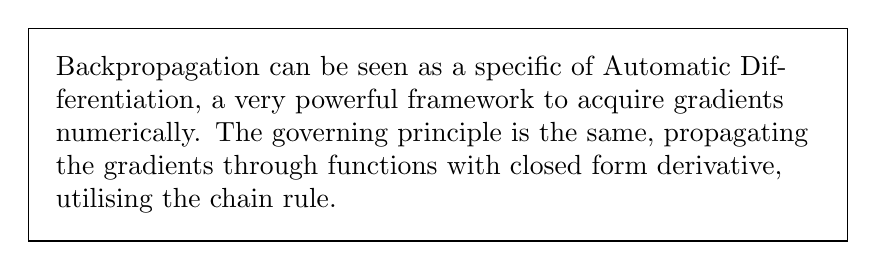
\begin{tikzpicture}
        \node [rectangle, draw, text width=0.8\textwidth, inner sep=10pt] (content) at (0,0) {
            Backpropagation can be seen as a specific of Automatic Differentiation, a very powerful framework to acquire gradients numerically.
            The governing principle is the same, propagating the gradients through functions with closed form derivative, utilising the chain rule.
        };
    \end{tikzpicture}

    \subsection{Neural ODEs}
    Calculating $\nabla_{\theta}L$ in neural ODEs can be achieved by differentiating through the solver steps but as we will demonstrate there is a much more efficient way, using tools from optimal control theory, namely adjoint sensitivities.
    The governing equations for neural ODEs are~\eqref{ivp},~\eqref{adjoint},~\eqref{dldtheta} we repeat them for convenience:

    \begin{equation*}
        \pmb{y}(T) =  \pmb{y}(0) +\int_{0}^{T} f(\pmb{y}(\tau), \tau, \pmb{\theta}) \,d\tau
        , \quad
        \pmb{y}(0) = \pmb{y}_0
    \end{equation*}

    \begin{equation*}
        \frac
        {d \pmb{a}(t)}
        {dt}
        =
        - \pmb{a}(t)^T
        \frac
        {\partial f( \pmb{y}(t), t, \pmb{\theta} )}
        {\partial \pmb{y} }
        , \quad
        \pmb{a}(T) = \frac{\partial L}{\partial \pmb{y}(T)}
    \end{equation*}

    \begin{equation*}
        \nabla_{\pmb{\theta}} L =
        - \int_T^0
        \pmb{a}(t)^T
        \frac
        {\partial f(\pmb{y}(\tau), \pmb{\theta})}
        {\partial \pmb{\theta}}
        \, d\tau
    \end{equation*}

    Calculating the last integral numerically requires the values of $\pmb{a}(t)$ at all the points in time the solver chooses.
    In the case of a fixed step size solver with step $h$ those would be $t_m = T - mh, \; m=0,1,\dots$.
    In the case of an adaptive step size $t_m$ could be any point between $T$ and $0$.
    In both cases we can calculate those quantities by solving the second ODE starting from time $t=T$ -where $a(T)$ has a closed form solution- and moving backwards in time.
    Next we need the value of $\pmb{y}$ at the same $t_m$s. Again we can calculate them starting from $\pmb{y}(T)$ and solving the original IVP again backwards in time.
    Notice that we don't need to save any intermediate state or activations from the forward pass since we can re-calculate them moving backwards.
    In this sense, neural ODEs are reversible (up to numerical tolerances).

    In algorithm~\ref{alg:adjoint} we reformulate the integral equation for the gradient of the loss wrt.
    weights as a differential equation: $ \frac{d}{dt} \pmb{a}_\theta(t) = -\pmb{a}(t)^T \frac{\partial f}{\partial \pmb{\theta}}$.
    We know that $\pmb{a}_\theta(T) = 0$ and we search for $\pmb{a}_\theta(0) = \nabla_\theta L$.

    \begin{algorithm}
        \caption{Adjoint}
        \label{alg:adjoint}
        \begin{algorithmic}
            \State Choose ODE solver hyperparameters ($h$, $\dots$)
            \State Do the forward pass, find $\pmb{y}(T)$
            \State $\pmb{a}(T) \gets \frac{\partial L}{\partial \pmb{y}(T)}$ (closed form)
            \State $\pmb{a}_{\theta}(T) \gets 0$
            \State $t \gets T$
            \While{$t > 0$}
                \State $\pmb{y}(t - \Delta t) \gets \text{IntStep}(\pmb{y}(t), f) $
                \State $\pmb{a}(t - \Delta t) \gets \text{IntStep}(
                \pmb{a}(t), -\pmb{a}(t) \frac{\partial f }{\partial \pmb{y}}
                )$
                \State $\pmb{a}_{\theta}(t - \Delta t) \gets \text{IntStep}(
                \pmb{a}_{\theta}(t), -\pmb{a}(t) \frac{\partial f }{\partial \pmb{\theta}}
                )$
                \State $t \gets t - \Delta t$
            \EndWhile
            \State \textbf{return} $\pmb{a}_\theta(0) = \nabla_\theta L$
        \end{algorithmic}
    \end{algorithm}


    \section{Numerical Solvers}

    \subsection{Runge-Kutta 5}

    solve $\frac{dy}{dt} = f(t,y)$, $y(t_0) = y_0 $

    \begin{align*}
        y_{n+1} &= y_n + \frac{h}{6}(k_1 + 2k_2 +2k_3 + k_4)  \\
        t_{n+1} &= t_n + h
    \end{align*}

    \begin{align*}
        k_{1} &= f(t_{n}, y_{n}), \\
        k_{2} &= f(t_{n} + \frac{h}{2}, y_{n} + h \frac{ k_{1} }{ 2 } ),    \\
        k_{3} &= f(t_{n} + \frac{h}{2}, y_{n} + h \frac{ k_{2} }{ 2 } ),  \\
        k_{4} &= f(t_{n} + h, y_{n} + hk_3), \\
    \end{align*}

    can be proved using taylor series expansion...


    \section{An alternative derivation for $\frac{dL}{d \pmb{\theta}}$}
    \label{adjoint_proof}
    There are already many ways in the literature for finding this quantity without delving into control theory and reverse sensitivities.
    Intuitively in can be thought as a continuous analogous to classical backpropagation.

    \begin{align}
        \text{classical} &\to
        \frac{d L}{ d \pmb{\theta}} =
        \sum_k
        \frac{\partial L}{\partial \pmb{y}_{k}}
        \frac{\partial f(\pmb{y}_k, \pmb\theta)}{\partial \pmb{\theta}}
        \\
        \text{adjoint sensitivities} &\to
        \frac{d L}{ d \pmb{\theta}} =
        \int_T^0
        \frac{\partial L}{\partial \pmb{y}(\tau)}
        \frac{\partial f(\pmb{y}(\tau), \pmb{\theta})}{\partial \pmb{\theta}} \, d\tau
    \end{align}

    In the original neural ODEs paper~\cite{chen2018neural} the authors prove~\eqref{adjoint} and use an augmented state to prove~\eqref{dldtheta} while others like~\cite{kidger2022neural} provide alternative proofs.
    We present another, in our opinion much simpler, derivation for~\eqref{dldtheta}.
    Consider the more general case where the loss is dependant on intermediate state on a point $s \in (0,T)$.
    This is equivalent to the usual case where the loss depends only on the output state with $\mathcal{L}(s) = L(\pmb{y}(s))=0$ for $s\neq T$.
    Moreover, the state $\pmb{y}$ is a also dependant on the weights even though it's not explicitly written.

    \begin{align*}
        \frac{ d L(\bm{y}(s, \bm{\theta})) }{ d \bm{\theta} }
        &= \int_0^s \frac{d}{dt} \left( \frac{ d L(\bm{y}(s, \bm{\theta})}{ d \bm{\theta}} \right) dt \\
        &= \int_0^s \frac{d}{dt} \left( \frac{ d L(\bm{y}(t, \bm{\theta})}{ d \bm{y}(t)} \frac{d \bm{y}(t)}{d\bm{\theta}} \right) dt \\
        &= \int_0^s
        \frac{d}{dt} \frac{ d L(\bm{y}(t, \bm{\theta})}{ d \bm{y}(t)} \cdot \frac{d \bm{y}(t)}{d\bm{\theta}}
        +
        \frac{ d L(\bm{y}(t, \bm{\theta})}{ d \bm{y}(t)} \cdot \frac{d}{dt} \frac{d \bm{y}(t)}{d\bm{\theta}}
        dt \\
        &= \int_0^s
        \dot{\bm{a}}(t) \frac{d \bm{y}(t)}{d\bm{\theta}}
        +
        \bm{a}(t) \cdot \frac{d}{d\bm{\theta}} \frac{d \bm{y}(t)}{dt}
        dt \\
        &= \int_0^s
        \dot{\bm{a}}(t) \frac{d \bm{y}(t)}{d\bm{\theta}}
        +
        \bm{a}(t) \cdot \frac{d\bm{f}}{d\theta}
        dt \\
        &= \int_0^s
        \dot{\bm{a}}(t) \frac{d \bm{y}(t)}{d\bm{\theta}}
        +
        \bm{a}(t) \left( \frac{\partial \bm{f}}{\partial \bm{\theta}}
        +
        \frac{\partial \bm{f}}{\partial \bm{y}(t)} \frac{\partial \bm{y}(t)}{\partial \bm{\theta}}\right)
        dt \\
        &= \int_0^s
        \frac{d \bm{y}(t)}{d\bm{\theta}}
        \left( \dot{\bm{a}}(t) + a\frac{\partial \bm{f}}{\partial \bm{y}(t)} \right)
        +
        \bm{a}(t) \frac{\partial \bm{f}}{\partial \bm{\theta}}
        dt \\
    \end{align*}
    From~\eqref{adjoint} the sum in the parenthesis is 0:
    \begin{align}
        \frac{ d L(\bm{y}(s, \bm{\theta})) }{ d \bm{\theta} }
        = \int_0^s
        \bm{a}(t) \frac{\partial \bm{f}}{\partial \bm{\theta}}
        dt
    \end{align}
    Setting $s=T$ we arrive at the desired formula.


    \section{Vector-Jacobian products}
    Modern software packages utilise automatic differentiation methods to calculate derivatives of some arbitrary function $f$, usually with respect to some parameters or weights $\theta$.
    \begin{equation}
        \frac{\partial f(x; \theta)}{ \partial \theta}
    \end{equation}


    \section{Optimisation}
    In the field of numerical optimisation many methods have been developed for minimising a \textit{scalar} objective function $f$.
    One category of those, \textit{line search} methods, are iterative algorithms that seek to update the current iterate $x_k$ to a new value closer to the minimum.
    They work by choosing a direction $p_k$ -and step size $\alpha$- along which $f$ is decreased.
    Alternatively the problem can be restated as:
    \begin{equation}
        \min_{a>0} f(x_k + \alpha p_k) \label{min_a}
    \end{equation}
    While ideally we would solve~\eqref{min_a} exactly, in practice it is computationally expensive and practically unnecessary.
    Line search implementations usually generate some trial step sizes until they find one that satisfies certain termination conditions we will examine later.

    A \textit{descent direction} is a direction that causes $f$ to decrease along it given sufficiently small $\alpha > 0$: $f(x_k + \alpha p_k) < f(x_k)$.We can show that if $p_k$ is a descent direction then $p_k^T \nabla f_k < 0$.
    From the first order Taylor series expansion we have:
    \begin{equation*}
        f(x_k+ap_k) = f(x_k) + a p_k^T \nabla f_k + O(a^2)< f(x_k) \\
    \end{equation*}
    Ignoring quadratic term since $\alpha$ is small.
    \begin{align*}
        a p_k^T \nabla f_k &< 0 \\
        p_k^T \nabla f_k &< 0
    \end{align*}
    It can be proven though Zoutendijk's theorem that: as long as the search direction is a descent direction and the step size fulfils some conditions the algorithm is globally convergent.

    The defining characteristic of a line search method is the way in which we obtain the search direction $p_k$.
    An obvious choice is to use the direction of \textit{steepest descent}, mathematically obtained as the negative of the gradient at the current iterate.
    \begin{equation}
        x_{k+1} = x_k - \alpha \nabla f_k
    \end{equation}

    In machine learning literature steepest descent, or as they are more commonly refereed, \textit{gradient descent} methods are extremely common.
    Almost all neural network models are trained using some derivative of classic gradient descent.
    These methods are not categorised as line searches since they do not seek to find an appropriate step length $\alpha$ on each iteration.
    They instead define either a fixed or dynamically updated \textit{learning rate}.
    Usually they employ some notions of momentum and stochasticity to move along a direction dictated by an approximation of the local gradient.
    Even so the remain first order methods since they only utilise information about the first derivative.
    Some notable gradient descent methods as well as how the minimisation problem is formulated in the context of machine learning are discussed later.

    \subsection{The Newton-Raphson algorithm with Hessian modification}
    \label{newtonalgo}
    In more general minimisation problems a prevalent search direction for line search optimisers is the \textit{Newton direction}, methods using this direction are called Newton methods.
    This direction is derived from the second-order Taylor series approximation of the objective function, near the current iterate $x_k$.
    Consider a continuous, twice differentiable function $f: \mathbb{R}^n \to \mathbb{R}^n$, its second order Taylor series approximation is:
    \begin{equation}
        f(x_k + p) = f_k + p^t \nabla f_k + \frac{1}{2} p^t \nabla^2 f_k p + R(p) \label{taylor}
    \end{equation}
    with $R(p)$ being of order $O(\rVert p \rVert^3)$.
    For small values of $p$, the residual term diminishes and we have a pretty good quadratic model of $f$.
    Seeking to minimise this model we set the derivative wrt. $p$ equal to 0:
    \begin{align}
        \nabla f_k + \nabla^2 f_k p_t &= 0  \label{grad_m} \\
        p = -\left[ \nabla^2 f_k \right]^{-1} \nabla f_k \label{newton_dir}
    \end{align}
    Equation~\eqref{newton_dir} gives the definition of the newton direction.
    As mentioned before, in order for the algorithm to be globally convergent the search direction has to be a descent direction.
    By multiplying~\eqref{grad_m} from the left with $p^t$ we get:
    \begin{align}
        p^t \nabla f_k + p_t \nabla^2 f_k p_t =& 0 \\
        p^t \nabla^2 f_k p_t =& -p^t \nabla f_k < 0 \\
        p^t \nabla^2 f_k p_t &> 0 \label{pos_def}
    \end{align}
    From~\eqref{pos_def} it is apparent that the Hessian matrix $H_k=\nabla^2 f_k$ has to be positive definite which is generally true if $x_k$ is near the minimum but not necessarily true away from it.
    If the Hessian is not positive definite there is no guarantee that~\eqref{newton_dir} gives a descent direction or even that the Hessian is non-singular.
    In order to address this issue a positive definite approximation of the Hessian is used.
    The approximation can be obtained in several ways, some involve adding a multiple of the identity or some correction matrix $\Delta H$, others modify the eigenvalues of the true Hessian directly.

    For example in~\cite{cheng1998modified} is shown that, if $H_k$ has spectral decomposition $H_k = Q \Lambda Q^T$ then the correction matrix of minimum Frobenius norm that ensures that the smallest eigenvalue of $H_k + \Delta H$ is larger or equal to $\delta$ is given by:
    \begin{equation*}
        \Delta H = Q \text(diag){\tau_i} Q^T, \quad \text{with} \quad \tau_i =
        \left\{
        \begin{array}{ll}
            0,                  & \lambda_i \geq \delta, \\
            \delta - \lambda_i, & \lambda_i < \delta,
        \end{array}
        \right.
    \end{equation*}

    Another technique, the one used here, is to perform (or try to perform) a Cholesky decomposition, more specifically an LDL decomposition of the Hessian.
    Since the Hessian is not always positive definite the factorisation $H = LDL^T$ may not exist or if even if it does the algorithm used to compute it is numerically unstable.
    The core idea of modified Cholesky decomposition is to modify the values of the diagonal matrix D to be sufficiently positive while the factorisation is computed.

    More specifically,~\cite{wright2006numerical} provide an algorithm for computing the $LDL^T$ factorisation a positive definite approximation of a matrix.
    It accepts two additional parameters $\delta, \beta$ so that the following bounds are satisfied.
    \begin{equation}
        d_j \geq \delta, \quad \lvert m_{ij} \rvert \leq \beta, \quad i = j+1, j_2, \dots, n
    \end{equation}

    The algorithm calculates the elements of the diagonal $D$ and the unitriangular matrix $L$ column by column.
    It is a simpler version of the algorithm presented by~\cite{gill2019practical} that additionally introduces symmetric row-column interchanges resulting in lower $ \lVert H_k - \hat{H}_k \rVert$, $\hat{H}_k$ being the approximation.

    \begin{algorithm}
        \caption{Modified Cholesky}
        \begin{algorithmic}
            \For{ $i = j+1,\dots,n$ }
                \State $c_{jj} \gets a_{jj} - \sum_{s=1}^{j-1} d_s l_{js}$
                \State $\theta_j \gets \max_{j<i\leq n}(\lvert c_{ij} \rvert)$
                \State $d_j \gets  \max
                \left(
                \lvert c_{jj} \rvert,
                \left( \frac{\theta_j}{\beta} \right)^2,
                \delta \right)$
                \For{$i = j+1,\dots, n$}
                    \State $c_{ij} \gets a_{ij} - \sum_{s=1}^{j-1} d_s l_{is} l_{js}$
                    \State $l_{ij} \gets c_{ij} / d_j$
                \EndFor
            \EndFor
        \end{algorithmic}
    \end{algorithm}

    After addressing the definiteness of the the Hessian let's describe how an algorithm would decide on the step size.
    As noted earlier Zoutendijk's theorem requires the search direction to be a descent direction as well as the step size to fulfil a certain set of conditions.
    One can prove Zoutedijk's theorem for multiple sets of conditions, namely the Wolfe, strong Wolfe and Goldstein conditions.
    We will focus on the strong Wolfe conditions.

    Assume we have chose direction $p_k$ at step $k$ of the algorithm, our second objective is to find step size $a$ to proceed to the next step without minimising $\phi(\alpha) = f(x_k + \alpha p_k)$ explicitly.
    The first strong Wolfe condition states that our guess for $a$ should give \textit{sufficient decrease} in the objective function in the following way:
    \begin{equation}
        f(x_k + ap_k) \leq f(x_k) + c_1 a \nabla f_k ^T p_k
    \end{equation}
    for some $c_1 \in (0,1)$ usually chosen to be quite small ($\approx 10^{-4}$). This ensures the reduction in $f$ is proportional to the step size as well as the directional derivative $\nabla f ^T p_k$.
    The sufficient decrease condition is not enough to make reasonable progress since it's satisfied for values of $\alpha$ close to 0.
    To prevent this, the second strong Wolfe condition or \textit{curvature condition} states that $\alpha$ should also satisfy:
    \begin{equation}
        \lvert \nabla f(x_k + \alpha p_k )^T p_k \rvert \leq \lvert c_2 \nabla f_k^T p_k \rvert
    \end{equation}
    for some constant $c_2 \in (c_1, 1)$ usually set around $0.9$ for Newton direction.
    Notice that the left hand side if the derivative wrt. $\alpha$ of $\phi(a)$ at $a_k$ and the right hand size at $0$.
    Practically the curvature condition requires the slope of $\phi$ at the new point to be greater that at the start times $c_2$.
    Remember that $p_k$ is a descent direction so $\phi(0)$ is strictly negative.
    Larger slope would mean we get closer to a stationary point of zero gradient.
    The absolute ensures that the slope doesn't become too positive and we don't overshoot away from the stationary point.

    Utilising those conditions we construct the following line search algorithm parameterised by $c_1, c_2, \alpha_{max}$

    \begin{algorithm}
        \caption{Line search}
        \label{alg:linesearh}
        \begin{algorithmic}
            \State Set $a_0 \gets 0$, choose $a_1 \in (0, a_{max})$
            \State $i \gets 1$
            \Repeat
                \If {$\phi(a_i) > \phi(0) + c_1 a_i \phi'(0)$ or [$\phi(a_i) \geq \phi(a_{i-1})$ and $i>1$]}
                    \State return \textbf{zoom}($a_{i-1}, a_i$)
                \EndIf
                \If {$\lvert \phi'(a_i) \rvert \leq -c_2 \phi'(0)$}
                    \State return $a_i$
                \EndIf
                \If {$\phi'(a_i) \geq 0$}
                    \State return \textbf{zoom}($a_i, a_{i-1}$)
                \EndIf
                \State $a_{i+1} \gets \min({a_max, 2*a_i})$
                \State $i \gets i+1$
            \Until
        \end{algorithmic}
    \end{algorithm}


\end{document}
